\documentclass[twoside]{book}

% Packages required by doxygen
\usepackage{fixltx2e}
\usepackage{calc}
\usepackage{doxygen}
\usepackage[export]{adjustbox} % also loads graphicx
\usepackage{graphicx}
\usepackage[utf8]{inputenc}
\usepackage{makeidx}
\usepackage{multicol}
\usepackage{multirow}
\PassOptionsToPackage{warn}{textcomp}
\usepackage{textcomp}
\usepackage[nointegrals]{wasysym}
\usepackage[table]{xcolor}

% Font selection
\usepackage[T1]{fontenc}
\usepackage[scaled=.90]{helvet}
\usepackage{courier}
\usepackage{amssymb}
\usepackage{sectsty}
\renewcommand{\familydefault}{\sfdefault}
\allsectionsfont{%
  \fontseries{bc}\selectfont%
  \color{darkgray}%
}
\renewcommand{\DoxyLabelFont}{%
  \fontseries{bc}\selectfont%
  \color{darkgray}%
}
\newcommand{\+}{\discretionary{\mbox{\scriptsize$\hookleftarrow$}}{}{}}

% Page & text layout
\usepackage{geometry}
\geometry{%
  a4paper,%
  top=2.5cm,%
  bottom=2.5cm,%
  left=2.5cm,%
  right=2.5cm%
}
\tolerance=750
\hfuzz=15pt
\hbadness=750
\setlength{\emergencystretch}{15pt}
\setlength{\parindent}{0cm}
\setlength{\parskip}{3ex plus 2ex minus 2ex}
\makeatletter
\renewcommand{\paragraph}{%
  \@startsection{paragraph}{4}{0ex}{-1.0ex}{1.0ex}{%
    \normalfont\normalsize\bfseries\SS@parafont%
  }%
}
\renewcommand{\subparagraph}{%
  \@startsection{subparagraph}{5}{0ex}{-1.0ex}{1.0ex}{%
    \normalfont\normalsize\bfseries\SS@subparafont%
  }%
}
\makeatother

% Headers & footers
\usepackage{fancyhdr}
\pagestyle{fancyplain}
\fancyhead[LE]{\fancyplain{}{\bfseries\thepage}}
\fancyhead[CE]{\fancyplain{}{}}
\fancyhead[RE]{\fancyplain{}{\bfseries\leftmark}}
\fancyhead[LO]{\fancyplain{}{\bfseries\rightmark}}
\fancyhead[CO]{\fancyplain{}{}}
\fancyhead[RO]{\fancyplain{}{\bfseries\thepage}}
\fancyfoot[LE]{\fancyplain{}{}}
\fancyfoot[CE]{\fancyplain{}{}}
\fancyfoot[RE]{\fancyplain{}{\bfseries\scriptsize Generated by Doxygen }}
\fancyfoot[LO]{\fancyplain{}{\bfseries\scriptsize Generated by Doxygen }}
\fancyfoot[CO]{\fancyplain{}{}}
\fancyfoot[RO]{\fancyplain{}{}}
\renewcommand{\footrulewidth}{0.4pt}
\renewcommand{\chaptermark}[1]{%
  \markboth{#1}{}%
}
\renewcommand{\sectionmark}[1]{%
  \markright{\thesection\ #1}%
}

% Indices & bibliography
\usepackage{natbib}
\usepackage[titles]{tocloft}
\setcounter{tocdepth}{3}
\setcounter{secnumdepth}{5}
\makeindex

% Hyperlinks (required, but should be loaded last)
\usepackage{ifpdf}
\ifpdf
  \usepackage[pdftex,pagebackref=true]{hyperref}
\else
  \usepackage[ps2pdf,pagebackref=true]{hyperref}
\fi
\hypersetup{%
  colorlinks=true,%
  linkcolor=blue,%
  citecolor=blue,%
  unicode%
}

% Custom commands
\newcommand{\clearemptydoublepage}{%
  \newpage{\pagestyle{empty}\cleardoublepage}%
}

\usepackage{caption}
\captionsetup{labelsep=space,justification=centering,font={bf},singlelinecheck=off,skip=4pt,position=top}

%===== C O N T E N T S =====

\begin{document}

% Titlepage & ToC
\hypersetup{pageanchor=false,
             bookmarksnumbered=true,
             pdfencoding=unicode
            }
\pagenumbering{roman}
\begin{titlepage}
\vspace*{7cm}
\begin{center}%
{\Large Trilinear }\\
\vspace*{1cm}
{\large Generated by Doxygen 1.8.11}\\
\end{center}
\end{titlepage}
\clearemptydoublepage
\tableofcontents
\clearemptydoublepage
\pagenumbering{arabic}
\hypersetup{pageanchor=true}

%--- Begin generated contents ---
\chapter{Hierarchical Index}
\section{Class Hierarchy}
This inheritance list is sorted roughly, but not completely, alphabetically\+:\begin{DoxyCompactList}
\item \contentsline{section}{\+\_\+socket}{\pageref{struct__socket}}{}
\item \contentsline{section}{Act\+Handler}{\pageref{classActHandler}}{}
\item \contentsline{section}{Basic\+Coach}{\pageref{classBasicCoach}}{}
\item \contentsline{section}{Basic\+Player}{\pageref{classBasicPlayer}}{}
\begin{DoxyCompactList}
\item \contentsline{section}{Player}{\pageref{classPlayer}}{}
\end{DoxyCompactList}
\item \contentsline{section}{Circle}{\pageref{classCircle}}{}
\item \contentsline{section}{Connection}{\pageref{classConnection}}{}
\item \contentsline{section}{Feature}{\pageref{classFeature}}{}
\item \contentsline{section}{Formations}{\pageref{classFormations}}{}
\item \contentsline{section}{Formation\+Type\+Info}{\pageref{classFormationTypeInfo}}{}
\item \contentsline{section}{Generic\+Values}{\pageref{classGenericValues}}{}
\begin{DoxyCompactList}
\item \contentsline{section}{Player\+Settings}{\pageref{classPlayerSettings}}{}
\item \contentsline{section}{Server\+Settings}{\pageref{classServerSettings}}{}
\end{DoxyCompactList}
\item \contentsline{section}{Generic\+ValueT}{\pageref{classGenericValueT}}{}
\item \contentsline{section}{Geometry}{\pageref{classGeometry}}{}
\item \contentsline{section}{Hetero\+Player\+Settings}{\pageref{classHeteroPlayerSettings}}{}
\item \contentsline{section}{Line}{\pageref{classLine}}{}
\item \contentsline{section}{Logger}{\pageref{classLogger}}{}
\item \contentsline{section}{Object}{\pageref{classObject}}{}
\begin{DoxyCompactList}
\item \contentsline{section}{Dynamic\+Object}{\pageref{classDynamicObject}}{}
\begin{DoxyCompactList}
\item \contentsline{section}{Ball\+Object}{\pageref{classBallObject}}{}
\item \contentsline{section}{Player\+Object}{\pageref{classPlayerObject}}{}
\begin{DoxyCompactList}
\item \contentsline{section}{Agent\+Object}{\pageref{classAgentObject}}{}
\end{DoxyCompactList}
\end{DoxyCompactList}
\item \contentsline{section}{Fixed\+Object}{\pageref{classFixedObject}}{}
\end{DoxyCompactList}
\item \contentsline{section}{Parse}{\pageref{classParse}}{}
\item \contentsline{section}{Player\+Type\+Info}{\pageref{classPlayerTypeInfo}}{}
\item \contentsline{section}{Rect}{\pageref{classRect}}{}
\item \contentsline{section}{Sense\+Handler}{\pageref{classSenseHandler}}{}
\item \contentsline{section}{Soccer\+Command}{\pageref{classSoccerCommand}}{}
\item \contentsline{section}{Soccer\+Types}{\pageref{classSoccerTypes}}{}
\item \contentsline{section}{Stamina}{\pageref{classStamina}}{}
\item \contentsline{section}{Time}{\pageref{classTime}}{}
\item \contentsline{section}{Timing}{\pageref{classTiming}}{}
\item \contentsline{section}{Vec\+Position}{\pageref{classVecPosition}}{}
\item \contentsline{section}{World\+Model}{\pageref{classWorldModel}}{}
\end{DoxyCompactList}

\chapter{Class Index}
\section{Class List}
Here are the classes, structs, unions and interfaces with brief descriptions\+:\begin{DoxyCompactList}
\item\contentsline{section}{\hyperlink{struct__socket}{\+\_\+socket} }{\pageref{struct__socket}}{}
\item\contentsline{section}{\hyperlink{classActHandler}{Act\+Handler} }{\pageref{classActHandler}}{}
\item\contentsline{section}{\hyperlink{classAgentObject}{Agent\+Object} }{\pageref{classAgentObject}}{}
\item\contentsline{section}{\hyperlink{classBallObject}{Ball\+Object} }{\pageref{classBallObject}}{}
\item\contentsline{section}{\hyperlink{classBasicCoach}{Basic\+Coach} }{\pageref{classBasicCoach}}{}
\item\contentsline{section}{\hyperlink{classBasicPlayer}{Basic\+Player} }{\pageref{classBasicPlayer}}{}
\item\contentsline{section}{\hyperlink{classCircle}{Circle} }{\pageref{classCircle}}{}
\item\contentsline{section}{\hyperlink{classConnection}{Connection} }{\pageref{classConnection}}{}
\item\contentsline{section}{\hyperlink{classDynamicObject}{Dynamic\+Object} }{\pageref{classDynamicObject}}{}
\item\contentsline{section}{\hyperlink{classFeature}{Feature} }{\pageref{classFeature}}{}
\item\contentsline{section}{\hyperlink{classFixedObject}{Fixed\+Object} }{\pageref{classFixedObject}}{}
\item\contentsline{section}{\hyperlink{classFormations}{Formations} }{\pageref{classFormations}}{}
\item\contentsline{section}{\hyperlink{classFormationTypeInfo}{Formation\+Type\+Info} }{\pageref{classFormationTypeInfo}}{}
\item\contentsline{section}{\hyperlink{classGenericValues}{Generic\+Values} }{\pageref{classGenericValues}}{}
\item\contentsline{section}{\hyperlink{classGenericValueT}{Generic\+ValueT} }{\pageref{classGenericValueT}}{}
\item\contentsline{section}{\hyperlink{classGeometry}{Geometry} }{\pageref{classGeometry}}{}
\item\contentsline{section}{\hyperlink{classHeteroPlayerSettings}{Hetero\+Player\+Settings} }{\pageref{classHeteroPlayerSettings}}{}
\item\contentsline{section}{\hyperlink{classLine}{Line} }{\pageref{classLine}}{}
\item\contentsline{section}{\hyperlink{classLogger}{Logger} }{\pageref{classLogger}}{}
\item\contentsline{section}{\hyperlink{classObject}{Object} }{\pageref{classObject}}{}
\item\contentsline{section}{\hyperlink{classParse}{Parse} }{\pageref{classParse}}{}
\item\contentsline{section}{\hyperlink{classPlayer}{Player} }{\pageref{classPlayer}}{}
\item\contentsline{section}{\hyperlink{classPlayerObject}{Player\+Object} }{\pageref{classPlayerObject}}{}
\item\contentsline{section}{\hyperlink{classPlayerSettings}{Player\+Settings} }{\pageref{classPlayerSettings}}{}
\item\contentsline{section}{\hyperlink{classPlayerTypeInfo}{Player\+Type\+Info} }{\pageref{classPlayerTypeInfo}}{}
\item\contentsline{section}{\hyperlink{classRect}{Rect} }{\pageref{classRect}}{}
\item\contentsline{section}{\hyperlink{classSenseHandler}{Sense\+Handler} }{\pageref{classSenseHandler}}{}
\item\contentsline{section}{\hyperlink{classServerSettings}{Server\+Settings} }{\pageref{classServerSettings}}{}
\item\contentsline{section}{\hyperlink{classSoccerCommand}{Soccer\+Command} }{\pageref{classSoccerCommand}}{}
\item\contentsline{section}{\hyperlink{classSoccerTypes}{Soccer\+Types} }{\pageref{classSoccerTypes}}{}
\item\contentsline{section}{\hyperlink{classStamina}{Stamina} }{\pageref{classStamina}}{}
\item\contentsline{section}{\hyperlink{classTime}{Time} }{\pageref{classTime}}{}
\item\contentsline{section}{\hyperlink{classTiming}{Timing} }{\pageref{classTiming}}{}
\item\contentsline{section}{\hyperlink{classVecPosition}{Vec\+Position} }{\pageref{classVecPosition}}{}
\item\contentsline{section}{\hyperlink{classWorldModel}{World\+Model} }{\pageref{classWorldModel}}{}
\end{DoxyCompactList}

\chapter{File Index}
\section{File List}
Here is a list of all documented files with brief descriptions\+:\begin{DoxyCompactList}
\item\contentsline{section}{src/\hyperlink{ActHandler_8cpp}{Act\+Handler.\+cpp} }{\pageref{ActHandler_8cpp}}{}
\item\contentsline{section}{src/\hyperlink{ActHandler_8h}{Act\+Handler.\+h} }{\pageref{ActHandler_8h}}{}
\item\contentsline{section}{src/\hyperlink{BasicCoach_8cpp}{Basic\+Coach.\+cpp} }{\pageref{BasicCoach_8cpp}}{}
\item\contentsline{section}{src/\hyperlink{BasicCoach_8h}{Basic\+Coach.\+h} }{\pageref{BasicCoach_8h}}{}
\item\contentsline{section}{src/\hyperlink{BasicPlayer_8cpp}{Basic\+Player.\+cpp} }{\pageref{BasicPlayer_8cpp}}{}
\item\contentsline{section}{src/\hyperlink{BasicPlayer_8h}{Basic\+Player.\+h} }{\pageref{BasicPlayer_8h}}{}
\item\contentsline{section}{src/\hyperlink{Connection_8cpp}{Connection.\+cpp} }{\pageref{Connection_8cpp}}{}
\item\contentsline{section}{src/\hyperlink{Connection_8h}{Connection.\+h} }{\pageref{Connection_8h}}{}
\item\contentsline{section}{src/\hyperlink{Formations_8cpp}{Formations.\+cpp} }{\pageref{Formations_8cpp}}{}
\item\contentsline{section}{src/\hyperlink{Formations_8h}{Formations.\+h} }{\pageref{Formations_8h}}{}
\item\contentsline{section}{src/\hyperlink{GenericValues_8cpp}{Generic\+Values.\+cpp} }{\pageref{GenericValues_8cpp}}{}
\item\contentsline{section}{src/\hyperlink{GenericValues_8h}{Generic\+Values.\+h} }{\pageref{GenericValues_8h}}{}
\item\contentsline{section}{src/\hyperlink{Geometry_8cpp}{Geometry.\+cpp} }{\pageref{Geometry_8cpp}}{}
\item\contentsline{section}{src/\hyperlink{Geometry_8h}{Geometry.\+h} }{\pageref{Geometry_8h}}{}
\item\contentsline{section}{src/\hyperlink{Logger_8cpp}{Logger.\+cpp} }{\pageref{Logger_8cpp}}{}
\item\contentsline{section}{src/\hyperlink{Logger_8h}{Logger.\+h} }{\pageref{Logger_8h}}{}
\item\contentsline{section}{src/\hyperlink{main_8cpp}{main.\+cpp} }{\pageref{main_8cpp}}{}
\item\contentsline{section}{src/\hyperlink{mainCoach_8cpp}{main\+Coach.\+cpp} }{\pageref{mainCoach_8cpp}}{}
\item\contentsline{section}{src/\hyperlink{Objects_8cpp}{Objects.\+cpp} }{\pageref{Objects_8cpp}}{}
\item\contentsline{section}{src/\hyperlink{Objects_8h}{Objects.\+h} }{\pageref{Objects_8h}}{}
\item\contentsline{section}{src/\hyperlink{Parse_8cpp}{Parse.\+cpp} }{\pageref{Parse_8cpp}}{}
\item\contentsline{section}{src/\hyperlink{Parse_8h}{Parse.\+h} }{\pageref{Parse_8h}}{}
\item\contentsline{section}{src/\hyperlink{Player_8cpp}{Player.\+cpp} }{\pageref{Player_8cpp}}{}
\item\contentsline{section}{src/\hyperlink{Player_8h}{Player.\+h} }{\pageref{Player_8h}}{}
\item\contentsline{section}{src/\hyperlink{PlayerSettings_8cpp}{Player\+Settings.\+cpp} }{\pageref{PlayerSettings_8cpp}}{}
\item\contentsline{section}{src/\hyperlink{PlayerSettings_8h}{Player\+Settings.\+h} }{\pageref{PlayerSettings_8h}}{}
\item\contentsline{section}{src/\hyperlink{PlayerTeams_8cpp}{Player\+Teams.\+cpp} }{\pageref{PlayerTeams_8cpp}}{}
\item\contentsline{section}{src/\hyperlink{SenseHandler_8cpp}{Sense\+Handler.\+cpp} }{\pageref{SenseHandler_8cpp}}{}
\item\contentsline{section}{src/\hyperlink{SenseHandler_8h}{Sense\+Handler.\+h} }{\pageref{SenseHandler_8h}}{}
\item\contentsline{section}{src/\hyperlink{ServerSettings_8cpp}{Server\+Settings.\+cpp} }{\pageref{ServerSettings_8cpp}}{}
\item\contentsline{section}{src/\hyperlink{ServerSettings_8h}{Server\+Settings.\+h} }{\pageref{ServerSettings_8h}}{}
\item\contentsline{section}{src/\hyperlink{SoccerTypes_8cpp}{Soccer\+Types.\+cpp} }{\pageref{SoccerTypes_8cpp}}{}
\item\contentsline{section}{src/\hyperlink{SoccerTypes_8h}{Soccer\+Types.\+h} }{\pageref{SoccerTypes_8h}}{}
\item\contentsline{section}{src/\hyperlink{WorldModel_8cpp}{World\+Model.\+cpp} }{\pageref{WorldModel_8cpp}}{}
\item\contentsline{section}{src/\hyperlink{WorldModel_8h}{World\+Model.\+h} }{\pageref{WorldModel_8h}}{}
\item\contentsline{section}{src/\hyperlink{WorldModelHighLevel_8cpp}{World\+Model\+High\+Level.\+cpp} }{\pageref{WorldModelHighLevel_8cpp}}{}
\item\contentsline{section}{src/\hyperlink{WorldModelPredict_8cpp}{World\+Model\+Predict.\+cpp} }{\pageref{WorldModelPredict_8cpp}}{}
\item\contentsline{section}{src/\hyperlink{WorldModelUpdate_8cpp}{World\+Model\+Update.\+cpp} }{\pageref{WorldModelUpdate_8cpp}}{}
\end{DoxyCompactList}

\chapter{Class Documentation}
\hypertarget{struct__socket}{}\section{\+\_\+socket Struct Reference}
\label{struct__socket}\index{\+\_\+socket@{\+\_\+socket}}


{\ttfamily \#include $<$Connection.\+h$>$}

\subsection*{Public Attributes}
\begin{DoxyCompactItemize}
\item 
int \hyperlink{struct__socket_a59af0d6587e9d93fd48cd19bc22e1bec}{socketfd}
\item 
struct sockaddr\+\_\+in \hyperlink{struct__socket_a68179c318bad7971ce3dc350b89439c4}{serv\+\_\+addr}
\end{DoxyCompactItemize}


\subsection{Detailed Description}
Socket is a combination of a filedescriptor with a server adress. 

\subsection{Member Data Documentation}
\index{\+\_\+socket@{\+\_\+socket}!serv\+\_\+addr@{serv\+\_\+addr}}
\index{serv\+\_\+addr@{serv\+\_\+addr}!\+\_\+socket@{\+\_\+socket}}
\subsubsection[{\texorpdfstring{serv\+\_\+addr}{serv_addr}}]{\setlength{\rightskip}{0pt plus 5cm}struct sockaddr\+\_\+in \+\_\+socket\+::serv\+\_\+addr}\hypertarget{struct__socket_a68179c318bad7971ce3dc350b89439c4}{}\label{struct__socket_a68179c318bad7971ce3dc350b89439c4}
Server information of the socket. \index{\+\_\+socket@{\+\_\+socket}!socketfd@{socketfd}}
\index{socketfd@{socketfd}!\+\_\+socket@{\+\_\+socket}}
\subsubsection[{\texorpdfstring{socketfd}{socketfd}}]{\setlength{\rightskip}{0pt plus 5cm}int \+\_\+socket\+::socketfd}\hypertarget{struct__socket_a59af0d6587e9d93fd48cd19bc22e1bec}{}\label{struct__socket_a59af0d6587e9d93fd48cd19bc22e1bec}
File descriptor of the socket. 

The documentation for this struct was generated from the following file\+:\begin{DoxyCompactItemize}
\item 
src/\hyperlink{Connection_8h}{Connection.\+h}\end{DoxyCompactItemize}

\hypertarget{classActHandler}{}\section{Act\+Handler Class Reference}
\label{classActHandler}\index{Act\+Handler@{Act\+Handler}}


{\ttfamily \#include $<$Act\+Handler.\+h$>$}

\subsection*{Public Member Functions}
\begin{DoxyCompactItemize}
\item 
\hyperlink{classActHandler_a33150037eae151edb5b068f2e72578c6}{Act\+Handler} (\hyperlink{classConnection}{Connection} $\ast$c, \hyperlink{classWorldModel}{World\+Model} $\ast$wm, \hyperlink{classServerSettings}{Server\+Settings} $\ast$ss)
\item 
bool \hyperlink{classActHandler_a898c8d843a88987196c8ea6a0ed18dec}{put\+Command\+In\+Queue} (\hyperlink{classSoccerCommand}{Soccer\+Command} command)
\item 
void \hyperlink{classActHandler_aaeab199c583cfe59252a5a7362d5b323}{empty\+Queue} ()
\item 
bool \hyperlink{classActHandler_a6c3bd023bea79f7cb7e8d2662641833a}{is\+Queue\+Empty} ()
\item 
bool \hyperlink{classActHandler_ab02a24e7c74fcaec56b0991a919a5e2e}{send\+Commands} ()
\item 
\hyperlink{classSoccerCommand}{Soccer\+Command} \hyperlink{classActHandler_a8ec983b87912733c9c2157e7d260fe57}{get\+Primary\+Command} ()
\item 
bool \hyperlink{classActHandler_a20294f4c12fb509bf05190942c7230cb}{send\+Command} (\hyperlink{classSoccerCommand}{Soccer\+Command} soc)
\item 
bool \hyperlink{classActHandler_aeb11ace593effbc3ac8cbbeb8bdafe69}{send\+Message} (char $\ast$str)
\item 
bool \hyperlink{classActHandler_a50f4ef305e795ed8714b7051dfda5916}{send\+Command\+Direct} (\hyperlink{classSoccerCommand}{Soccer\+Command} soc)
\item 
bool \hyperlink{classActHandler_a18b509f726900ddc2aaeb6accba9384e}{send\+Message\+Direct} (const char $\ast$str)
\end{DoxyCompactItemize}


\subsection{Detailed Description}
The \hyperlink{classActHandler}{Act\+Handler} Class is used in the Robo\+Cup Soccer environment to send the commands to the soccerserver. The \hyperlink{classActHandler}{Act\+Handler} contains a queue in which the commands are put. When a signal arrives (set by the \hyperlink{classSenseHandler}{Sense\+Handler} depending on the time of the sense\+\_\+body message) the commands that are currently in the queue are converted to text strings and send to the server. The sent commands are also passed to the \hyperlink{classWorldModel}{World\+Model}, such that the \hyperlink{classWorldModel}{World\+Model} can update its internal state based on the performed actions. It is possible to send more than one command to the server at each time step, but some type of (primary) commands can only be sent once (kick,dash, move, tackle, turn and catch). Therefore internally different queues are stored. One with only one element, namely the last entered primary command. One with all the change\+\_\+view commands (since these have to be sent at special times for the synchronization). And finally a separate queue containing all the other commands. Each time a command is put into the queue that is already there, the command is updated with the new information. Furthermore it is also possible to directly send commands (or text strings) to the server. These methods can be used when an initialization or move command has to be sent to the server and you\textquotesingle{}re sure this information is final, i.\+e. the message will not become better when new information arrives from the server. 

\subsection{Constructor \& Destructor Documentation}
\index{Act\+Handler@{Act\+Handler}!Act\+Handler@{Act\+Handler}}
\index{Act\+Handler@{Act\+Handler}!Act\+Handler@{Act\+Handler}}
\subsubsection[{\texorpdfstring{Act\+Handler(\+Connection $\ast$c, World\+Model $\ast$wm, Server\+Settings $\ast$ss)}{ActHandler(Connection *c, WorldModel *wm, ServerSettings *ss)}}]{\setlength{\rightskip}{0pt plus 5cm}Act\+Handler\+::\+Act\+Handler (
\begin{DoxyParamCaption}
\item[{{\bf Connection} $\ast$}]{c, }
\item[{{\bf World\+Model} $\ast$}]{wm, }
\item[{{\bf Server\+Settings} $\ast$}]{ss}
\end{DoxyParamCaption}
)}\hypertarget{classActHandler_a33150037eae151edb5b068f2e72578c6}{}\label{classActHandler_a33150037eae151edb5b068f2e72578c6}
This is the constructor for the \hyperlink{classActHandler}{Act\+Handler} class. All the variables are initialized. 
\begin{DoxyParams}{Parameters}
{\em c} & \hyperlink{classConnection}{Connection} that is connected with the soccerserver \\
\hline
{\em wm} & \hyperlink{classWorldModel}{World\+Model}, used to set performed commands \\
\hline
{\em ss} & \hyperlink{classServerSettings}{Server\+Settings} in which server settings are defined \\
\hline
\end{DoxyParams}


\subsection{Member Function Documentation}
\index{Act\+Handler@{Act\+Handler}!empty\+Queue@{empty\+Queue}}
\index{empty\+Queue@{empty\+Queue}!Act\+Handler@{Act\+Handler}}
\subsubsection[{\texorpdfstring{empty\+Queue()}{emptyQueue()}}]{\setlength{\rightskip}{0pt plus 5cm}void Act\+Handler\+::empty\+Queue (
\begin{DoxyParamCaption}
{}
\end{DoxyParamCaption}
)}\hypertarget{classActHandler_aaeab199c583cfe59252a5a7362d5b323}{}\label{classActHandler_aaeab199c583cfe59252a5a7362d5b323}
This method empties the queue in which all the commands are stored. \index{Act\+Handler@{Act\+Handler}!get\+Primary\+Command@{get\+Primary\+Command}}
\index{get\+Primary\+Command@{get\+Primary\+Command}!Act\+Handler@{Act\+Handler}}
\subsubsection[{\texorpdfstring{get\+Primary\+Command()}{getPrimaryCommand()}}]{\setlength{\rightskip}{0pt plus 5cm}{\bf Soccer\+Command} Act\+Handler\+::get\+Primary\+Command (
\begin{DoxyParamCaption}
{}
\end{DoxyParamCaption}
)}\hypertarget{classActHandler_a8ec983b87912733c9c2157e7d260fe57}{}\label{classActHandler_a8ec983b87912733c9c2157e7d260fe57}
This method returns the primary command that is currently stored in the queue. \index{Act\+Handler@{Act\+Handler}!is\+Queue\+Empty@{is\+Queue\+Empty}}
\index{is\+Queue\+Empty@{is\+Queue\+Empty}!Act\+Handler@{Act\+Handler}}
\subsubsection[{\texorpdfstring{is\+Queue\+Empty()}{isQueueEmpty()}}]{\setlength{\rightskip}{0pt plus 5cm}bool Act\+Handler\+::is\+Queue\+Empty (
\begin{DoxyParamCaption}
{}
\end{DoxyParamCaption}
)}\hypertarget{classActHandler_a6c3bd023bea79f7cb7e8d2662641833a}{}\label{classActHandler_a6c3bd023bea79f7cb7e8d2662641833a}
This method returns whether the current queue contains no commands \begin{DoxyReturn}{Returns}
true when queue is empty, false otherwise 
\end{DoxyReturn}
\index{Act\+Handler@{Act\+Handler}!put\+Command\+In\+Queue@{put\+Command\+In\+Queue}}
\index{put\+Command\+In\+Queue@{put\+Command\+In\+Queue}!Act\+Handler@{Act\+Handler}}
\subsubsection[{\texorpdfstring{put\+Command\+In\+Queue(\+Soccer\+Command command)}{putCommandInQueue(SoccerCommand command)}}]{\setlength{\rightskip}{0pt plus 5cm}bool Act\+Handler\+::put\+Command\+In\+Queue (
\begin{DoxyParamCaption}
\item[{{\bf Soccer\+Command}}]{command}
\end{DoxyParamCaption}
)}\hypertarget{classActHandler_a898c8d843a88987196c8ea6a0ed18dec}{}\label{classActHandler_a898c8d843a88987196c8ea6a0ed18dec}
This method puts a \hyperlink{classSoccerCommand}{Soccer\+Command} in the queue. The last added command will be sent to the soccerserver when the method send\+Commands is performed. Normally this is done when a signal set by the \hyperlink{classSenseHandler}{Sense\+Handler} arrives. 
\begin{DoxyParams}{Parameters}
{\em command} & \hyperlink{classSoccerCommand}{Soccer\+Command} that should be put in the queue. \\
\hline
\end{DoxyParams}
\begin{DoxyReturn}{Returns}
true when command is added, false otherwise (queue is full) 
\end{DoxyReturn}
\index{Act\+Handler@{Act\+Handler}!send\+Command@{send\+Command}}
\index{send\+Command@{send\+Command}!Act\+Handler@{Act\+Handler}}
\subsubsection[{\texorpdfstring{send\+Command(\+Soccer\+Command soc)}{sendCommand(SoccerCommand soc)}}]{\setlength{\rightskip}{0pt plus 5cm}bool Act\+Handler\+::send\+Command (
\begin{DoxyParamCaption}
\item[{{\bf Soccer\+Command}}]{soc}
\end{DoxyParamCaption}
)}\hypertarget{classActHandler_a20294f4c12fb509bf05190942c7230cb}{}\label{classActHandler_a20294f4c12fb509bf05190942c7230cb}
This method sends a single command directly to the server. First a string is made from the \hyperlink{classSoccerCommand}{Soccer\+Command} and afterwards this string is send to the server using the method send\+Message. 
\begin{DoxyParams}{Parameters}
{\em soc} & \hyperlink{classSoccerCommand}{Soccer\+Command} that should be send to the server. \\
\hline
\end{DoxyParams}
\begin{DoxyReturn}{Returns}
true when message was sent, false otherwise 
\end{DoxyReturn}
\index{Act\+Handler@{Act\+Handler}!send\+Command\+Direct@{send\+Command\+Direct}}
\index{send\+Command\+Direct@{send\+Command\+Direct}!Act\+Handler@{Act\+Handler}}
\subsubsection[{\texorpdfstring{send\+Command\+Direct(\+Soccer\+Command soc)}{sendCommandDirect(SoccerCommand soc)}}]{\setlength{\rightskip}{0pt plus 5cm}bool Act\+Handler\+::send\+Command\+Direct (
\begin{DoxyParamCaption}
\item[{{\bf Soccer\+Command}}]{soc}
\end{DoxyParamCaption}
)}\hypertarget{classActHandler_a50f4ef305e795ed8714b7051dfda5916}{}\label{classActHandler_a50f4ef305e795ed8714b7051dfda5916}
This method sends a single command directly to the server. First a string is made from the \hyperlink{classSoccerCommand}{Soccer\+Command} and afterwards this string is send to the server using the method send\+Message\+Direct. 
\begin{DoxyParams}{Parameters}
{\em soc} & \hyperlink{classSoccerCommand}{Soccer\+Command} that should be send to the server. \\
\hline
\end{DoxyParams}
\begin{DoxyReturn}{Returns}
true when message was sent, false otherwise 
\end{DoxyReturn}
\index{Act\+Handler@{Act\+Handler}!send\+Commands@{send\+Commands}}
\index{send\+Commands@{send\+Commands}!Act\+Handler@{Act\+Handler}}
\subsubsection[{\texorpdfstring{send\+Commands()}{sendCommands()}}]{\setlength{\rightskip}{0pt plus 5cm}bool Act\+Handler\+::send\+Commands (
\begin{DoxyParamCaption}
{}
\end{DoxyParamCaption}
)}\hypertarget{classActHandler_ab02a24e7c74fcaec56b0991a919a5e2e}{}\label{classActHandler_ab02a24e7c74fcaec56b0991a919a5e2e}
This method converts all commands in the queue to text strings and sends these text strings to the server (connected by \hyperlink{classConnection}{Connection}). When the server didn\textquotesingle{}t execute the commands from the previous cycle (this information is stored in the \hyperlink{classWorldModel}{World\+Model}) the commands in the queue are not sent, since it is probably the case that these commands will be performed this cycle and we don\textquotesingle{}t want a clash (two commands in one cycle). In this case false is returned. \begin{DoxyReturn}{Returns}
true when sending of messages succeeded, false otherwise 
\end{DoxyReturn}
\index{Act\+Handler@{Act\+Handler}!send\+Message@{send\+Message}}
\index{send\+Message@{send\+Message}!Act\+Handler@{Act\+Handler}}
\subsubsection[{\texorpdfstring{send\+Message(char $\ast$str)}{sendMessage(char *str)}}]{\setlength{\rightskip}{0pt plus 5cm}bool Act\+Handler\+::send\+Message (
\begin{DoxyParamCaption}
\item[{char $\ast$}]{str}
\end{DoxyParamCaption}
)}\hypertarget{classActHandler_aeb11ace593effbc3ac8cbbeb8bdafe69}{}\label{classActHandler_aeb11ace593effbc3ac8cbbeb8bdafe69}
This method sends a single string directly to the server. To make sure this message arrives, the time of one complete cycle is waited before and after the message is sent. 
\begin{DoxyParams}{Parameters}
{\em str} & string that should be sent to the server \\
\hline
\end{DoxyParams}
\begin{DoxyReturn}{Returns}
true when message was sent, false otherwise 
\end{DoxyReturn}
\index{Act\+Handler@{Act\+Handler}!send\+Message\+Direct@{send\+Message\+Direct}}
\index{send\+Message\+Direct@{send\+Message\+Direct}!Act\+Handler@{Act\+Handler}}
\subsubsection[{\texorpdfstring{send\+Message\+Direct(const char $\ast$str)}{sendMessageDirect(const char *str)}}]{\setlength{\rightskip}{0pt plus 5cm}bool Act\+Handler\+::send\+Message\+Direct (
\begin{DoxyParamCaption}
\item[{const char $\ast$}]{str}
\end{DoxyParamCaption}
)}\hypertarget{classActHandler_a18b509f726900ddc2aaeb6accba9384e}{}\label{classActHandler_a18b509f726900ddc2aaeb6accba9384e}
This method sends a single string directly to the server. 
\begin{DoxyParams}{Parameters}
{\em str} & string that should be sent to the server \\
\hline
\end{DoxyParams}
\begin{DoxyReturn}{Returns}
true when message was sent, false otherwise 
\end{DoxyReturn}


The documentation for this class was generated from the following files\+:\begin{DoxyCompactItemize}
\item 
src/\hyperlink{ActHandler_8h}{Act\+Handler.\+h}\item 
src/\hyperlink{ActHandler_8cpp}{Act\+Handler.\+cpp}\end{DoxyCompactItemize}

\hypertarget{classAgentObject}{}\section{Agent\+Object Class Reference}
\label{classAgentObject}\index{Agent\+Object@{Agent\+Object}}


{\ttfamily \#include $<$Objects.\+h$>$}



Inheritance diagram for Agent\+Object\+:
\nopagebreak
\begin{figure}[H]
\begin{center}
\leavevmode
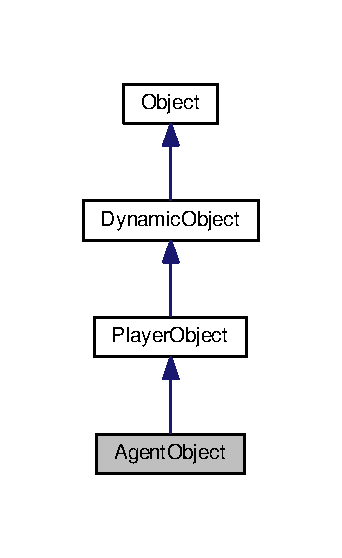
\includegraphics[width=164pt]{classAgentObject__inherit__graph}
\end{center}
\end{figure}


Collaboration diagram for Agent\+Object\+:
\nopagebreak
\begin{figure}[H]
\begin{center}
\leavevmode
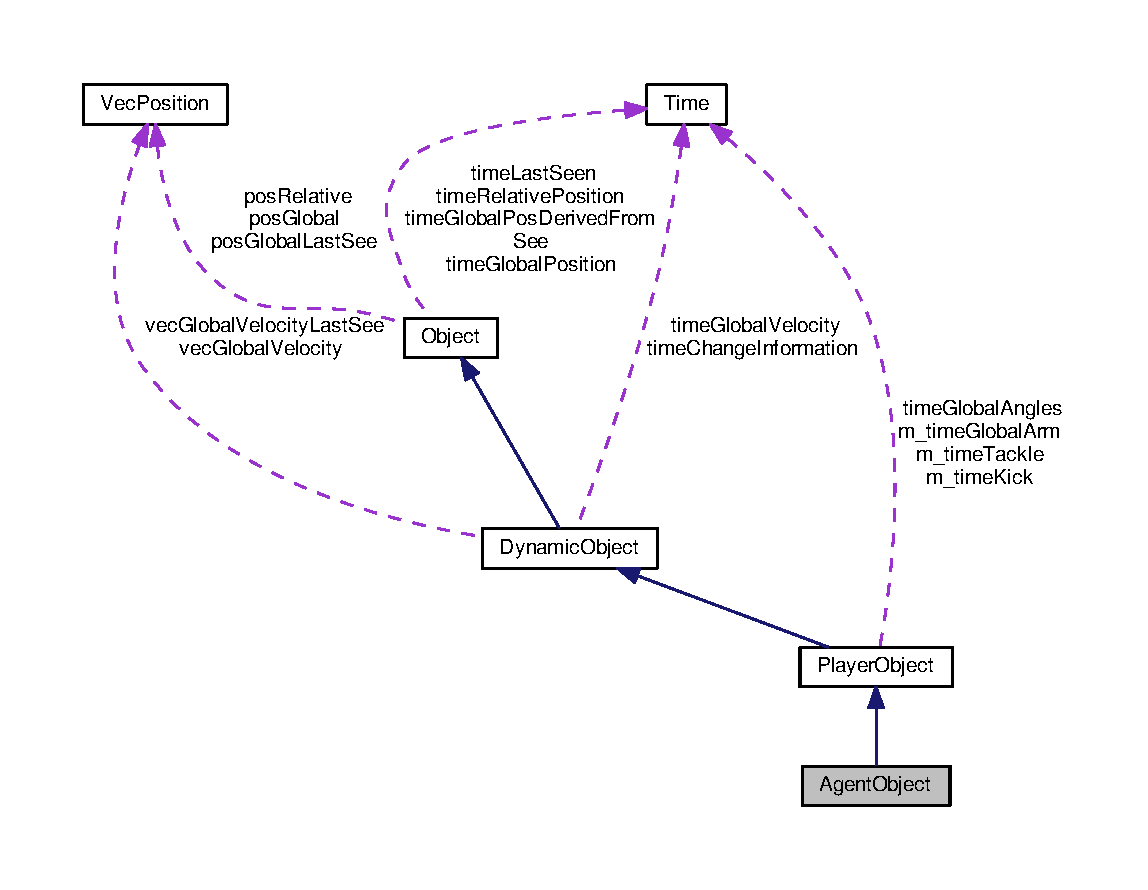
\includegraphics[width=350pt]{classAgentObject__coll__graph}
\end{center}
\end{figure}
\subsection*{Public Member Functions}
\begin{DoxyCompactItemize}
\item 
\hyperlink{classAgentObject_a46e0f4f9c495d64be7387425ac96c2ab}{Agent\+Object} (double d\+Stamina\+Max=4000)
\item 
void \hyperlink{classAgentObject_a0043cea8d237828930412eb3c2b84e32}{show} (ostream \&os=cout)
\item 
void \hyperlink{classAgentObject_ad486225386c1baa9218b5aa5d2045427}{show} (const char $\ast$str\+Team\+Name, ostream \&os=cout)
\item 
\hyperlink{classVecPosition}{Vec\+Position} \hyperlink{classAgentObject_a332c731bfaad817e328bab1906f59359}{get\+Position\+Difference} () const 
\item 
bool \hyperlink{classAgentObject_a982932ce580cbb643ed6be3f5c676351}{set\+Position\+Difference} (\hyperlink{classVecPosition}{Vec\+Position} v)
\item 
\hyperlink{SoccerTypes_8h_ade95094b8e117801bea82ec390cccf64}{View\+AngleT} \hyperlink{classAgentObject_a82da0c18490bd63868c3a399b168c8fd}{get\+View\+Angle} () const 
\item 
bool \hyperlink{classAgentObject_a55a226e986485f9f1995987eb4e6487b}{set\+View\+Angle} (\hyperlink{SoccerTypes_8h_ade95094b8e117801bea82ec390cccf64}{View\+AngleT} v)
\item 
\hyperlink{SoccerTypes_8h_a5ae52e4e8062de90b118eacb03e99906}{View\+QualityT} \hyperlink{classAgentObject_a9bd2e9ea93f7c9f4dadfb2e44496528d}{get\+View\+Quality} () const 
\item 
bool \hyperlink{classAgentObject_a40347ef44cedf172b2a8edebade46805}{set\+View\+Quality} (\hyperlink{SoccerTypes_8h_a5ae52e4e8062de90b118eacb03e99906}{View\+QualityT} v)
\item 
\hyperlink{classStamina}{Stamina} \hyperlink{classAgentObject_a167b9e6b5a2571f1886279dafbbb59d7}{get\+Stamina} () const 
\item 
bool \hyperlink{classAgentObject_a0f2ec1a68d2edbf1cda4cea847f9e5b8}{set\+Stamina} (\hyperlink{classStamina}{Stamina} sta)
\item 
\hyperlink{classVecPosition}{Vec\+Position} \hyperlink{classAgentObject_a05a81dbb6cefe6ad2b4548d084ad456b}{get\+Speed\+Rel\+To\+Neck} () const 
\item 
bool \hyperlink{classAgentObject_a9fe0db948cb05d01707e78b44e96c7f8}{set\+Speed\+Rel\+To\+Neck} (\hyperlink{classVecPosition}{Vec\+Position} v)
\item 
bool \hyperlink{classAgentObject_ae340af787802701523f55cd40555b93e}{set\+Global\+Neck\+Angle} (\hyperlink{Geometry_8h_a6bfe02ae9bb185092902092561ab2865}{Ang\+Deg} ang)
\item 
\hyperlink{Geometry_8h_a6bfe02ae9bb185092902092561ab2865}{Ang\+Deg} \hyperlink{classAgentObject_aa259adf422ce7d54ae7c94b20a44c2f4}{get\+Body\+Angle\+Rel\+To\+Neck} () const 
\item 
bool \hyperlink{classAgentObject_abe8da0bb6a593c714986abacc4e5ec1b}{set\+Body\+Angle\+Rel\+To\+Neck} (\hyperlink{Geometry_8h_a6bfe02ae9bb185092902092561ab2865}{Ang\+Deg} ang)
\item 
bool \hyperlink{classAgentObject_a8ee30512544a38fb49be8667e8ed0771}{get\+Arm\+Movable} () const 
\item 
bool \hyperlink{classAgentObject_aabacf8e03d85102c4f89da2420617ab0}{set\+Arm\+Movable} (bool b)
\item 
int \hyperlink{classAgentObject_a0c8a7da5056999e880824a822a5f0e52}{get\+Arm\+Expires} () const 
\item 
bool \hyperlink{classAgentObject_af0d42bee948a9f5f145a39e7caed4d46}{set\+Arm\+Expires} (int i)
\item 
\hyperlink{classVecPosition}{Vec\+Position} \hyperlink{classAgentObject_a1e30ba9c7314fd067e4783aaf481d134}{get\+Global\+Arm\+Position} () const 
\item 
bool \hyperlink{classAgentObject_a238bbacbf6083bbf1cfa1ff986aa9df5}{set\+Global\+Arm\+Position} (\hyperlink{classVecPosition}{Vec\+Position} v)
\item 
int \hyperlink{classAgentObject_a63e7f857385824d37e63aaa5f7caf117}{get\+Tackle\+Expires} () const 
\item 
bool \hyperlink{classAgentObject_a20855b8884bf0e247aeb402661803fd8}{set\+Tackle\+Expires} (int i)
\end{DoxyCompactItemize}
\subsection*{Additional Inherited Members}


\subsection{Detailed Description}
Class \hyperlink{classAgentObject}{Agent\+Object} contains Robo\+Cup information that is available for the agent. New variables are declared that extend a normal \hyperlink{classPlayerObject}{Player\+Object}. 

\subsection{Constructor \& Destructor Documentation}
\index{Agent\+Object@{Agent\+Object}!Agent\+Object@{Agent\+Object}}
\index{Agent\+Object@{Agent\+Object}!Agent\+Object@{Agent\+Object}}
\subsubsection[{\texorpdfstring{Agent\+Object(double d\+Stamina\+Max=4000)}{AgentObject(double dStaminaMax=4000)}}]{\setlength{\rightskip}{0pt plus 5cm}Agent\+Object\+::\+Agent\+Object (
\begin{DoxyParamCaption}
\item[{double}]{d\+Stamina\+Max = {\ttfamily 4000}}
\end{DoxyParamCaption}
)}\hypertarget{classAgentObject_a46e0f4f9c495d64be7387425ac96c2ab}{}\label{classAgentObject_a46e0f4f9c495d64be7387425ac96c2ab}
This is the constructor for the class \hyperlink{classAgentObject}{Agent\+Object} and initializes the variables with the \hyperlink{classAgentObject}{Agent\+Object}. This the class that contains information about the agent itself. 
\begin{DoxyParams}{Parameters}
{\em d\+Stamina\+Max} & maximum stamina for this agent (default 4000.\+0) \\
\hline
\end{DoxyParams}


\subsection{Member Function Documentation}
\index{Agent\+Object@{Agent\+Object}!get\+Arm\+Expires@{get\+Arm\+Expires}}
\index{get\+Arm\+Expires@{get\+Arm\+Expires}!Agent\+Object@{Agent\+Object}}
\subsubsection[{\texorpdfstring{get\+Arm\+Expires() const }{getArmExpires() const }}]{\setlength{\rightskip}{0pt plus 5cm}int Agent\+Object\+::get\+Arm\+Expires (
\begin{DoxyParamCaption}
{}
\end{DoxyParamCaption}
) const}\hypertarget{classAgentObject_a0c8a7da5056999e880824a822a5f0e52}{}\label{classAgentObject_a0c8a7da5056999e880824a822a5f0e52}
This method returns the numer of cycles it will take the arm to expire. In case of zero, the arm doesn\textquotesingle{}t point anymore and the other players won\textquotesingle{}t see the arm pointing anymore. \index{Agent\+Object@{Agent\+Object}!get\+Arm\+Movable@{get\+Arm\+Movable}}
\index{get\+Arm\+Movable@{get\+Arm\+Movable}!Agent\+Object@{Agent\+Object}}
\subsubsection[{\texorpdfstring{get\+Arm\+Movable() const }{getArmMovable() const }}]{\setlength{\rightskip}{0pt plus 5cm}bool Agent\+Object\+::get\+Arm\+Movable (
\begin{DoxyParamCaption}
{}
\end{DoxyParamCaption}
) const}\hypertarget{classAgentObject_a8ee30512544a38fb49be8667e8ed0771}{}\label{classAgentObject_a8ee30512544a38fb49be8667e8ed0771}
This method sets whether it is allowed to move the arm of the agent. \index{Agent\+Object@{Agent\+Object}!get\+Body\+Angle\+Rel\+To\+Neck@{get\+Body\+Angle\+Rel\+To\+Neck}}
\index{get\+Body\+Angle\+Rel\+To\+Neck@{get\+Body\+Angle\+Rel\+To\+Neck}!Agent\+Object@{Agent\+Object}}
\subsubsection[{\texorpdfstring{get\+Body\+Angle\+Rel\+To\+Neck() const }{getBodyAngleRelToNeck() const }}]{\setlength{\rightskip}{0pt plus 5cm}{\bf Ang\+Deg} Agent\+Object\+::get\+Body\+Angle\+Rel\+To\+Neck (
\begin{DoxyParamCaption}
{}
\end{DoxyParamCaption}
) const}\hypertarget{classAgentObject_aa259adf422ce7d54ae7c94b20a44c2f4}{}\label{classAgentObject_aa259adf422ce7d54ae7c94b20a44c2f4}
This method returns the relative angle of the body to the neck of this \hyperlink{classAgentObject}{Agent\+Object}. Example\+: global angle neck is 90 degrees and global body angle is 0, means that relative angle of body to neck is -\/90 degrees. \begin{DoxyReturn}{Returns}
relative body angle to the neck 
\end{DoxyReturn}
\index{Agent\+Object@{Agent\+Object}!get\+Global\+Arm\+Position@{get\+Global\+Arm\+Position}}
\index{get\+Global\+Arm\+Position@{get\+Global\+Arm\+Position}!Agent\+Object@{Agent\+Object}}
\subsubsection[{\texorpdfstring{get\+Global\+Arm\+Position() const }{getGlobalArmPosition() const }}]{\setlength{\rightskip}{0pt plus 5cm}{\bf Vec\+Position} Agent\+Object\+::get\+Global\+Arm\+Position (
\begin{DoxyParamCaption}
{}
\end{DoxyParamCaption}
) const}\hypertarget{classAgentObject_a1e30ba9c7314fd067e4783aaf481d134}{}\label{classAgentObject_a1e30ba9c7314fd067e4783aaf481d134}
This method returns the global position to which the arm points. If \textquotesingle{}get\+Arm\+Expires\textquotesingle{} returns zero, it means that the arm doesn\textquotesingle{}t point anymore and this value is invalid. \index{Agent\+Object@{Agent\+Object}!get\+Position\+Difference@{get\+Position\+Difference}}
\index{get\+Position\+Difference@{get\+Position\+Difference}!Agent\+Object@{Agent\+Object}}
\subsubsection[{\texorpdfstring{get\+Position\+Difference() const }{getPositionDifference() const }}]{\setlength{\rightskip}{0pt plus 5cm}{\bf Vec\+Position} Agent\+Object\+::get\+Position\+Difference (
\begin{DoxyParamCaption}
{}
\end{DoxyParamCaption}
) const}\hypertarget{classAgentObject_a332c731bfaad817e328bab1906f59359}{}\label{classAgentObject_a332c731bfaad817e328bab1906f59359}
This method returns the difference between the predicted global position of the agent and the actual derived global position. This difference can be used in determining the actual movement of other objects since the noise caused by the difference in the global position of the agent is then filtered out. \index{Agent\+Object@{Agent\+Object}!get\+Speed\+Rel\+To\+Neck@{get\+Speed\+Rel\+To\+Neck}}
\index{get\+Speed\+Rel\+To\+Neck@{get\+Speed\+Rel\+To\+Neck}!Agent\+Object@{Agent\+Object}}
\subsubsection[{\texorpdfstring{get\+Speed\+Rel\+To\+Neck() const }{getSpeedRelToNeck() const }}]{\setlength{\rightskip}{0pt plus 5cm}{\bf Vec\+Position} Agent\+Object\+::get\+Speed\+Rel\+To\+Neck (
\begin{DoxyParamCaption}
{}
\end{DoxyParamCaption}
) const}\hypertarget{classAgentObject_a05a81dbb6cefe6ad2b4548d084ad456b}{}\label{classAgentObject_a05a81dbb6cefe6ad2b4548d084ad456b}
This method returns the velocity (speed and direction) of this \hyperlink{classAgentObject}{Agent\+Object}. This information is directly availablefrom the sense message, in which the speed factor and the angle of this speed (relative to the neck) are given. \begin{DoxyReturn}{Returns}
velocity agent relative to the neck. 
\end{DoxyReturn}
\index{Agent\+Object@{Agent\+Object}!get\+Stamina@{get\+Stamina}}
\index{get\+Stamina@{get\+Stamina}!Agent\+Object@{Agent\+Object}}
\subsubsection[{\texorpdfstring{get\+Stamina() const }{getStamina() const }}]{\setlength{\rightskip}{0pt plus 5cm}{\bf Stamina} Agent\+Object\+::get\+Stamina (
\begin{DoxyParamCaption}
{}
\end{DoxyParamCaption}
) const}\hypertarget{classAgentObject_a167b9e6b5a2571f1886279dafbbb59d7}{}\label{classAgentObject_a167b9e6b5a2571f1886279dafbbb59d7}
This method returns the \hyperlink{classStamina}{Stamina} of the \hyperlink{classAgentObject}{Agent\+Object}. \begin{DoxyReturn}{Returns}
stamina from the agent. 
\end{DoxyReturn}
\index{Agent\+Object@{Agent\+Object}!get\+Tackle\+Expires@{get\+Tackle\+Expires}}
\index{get\+Tackle\+Expires@{get\+Tackle\+Expires}!Agent\+Object@{Agent\+Object}}
\subsubsection[{\texorpdfstring{get\+Tackle\+Expires() const }{getTackleExpires() const }}]{\setlength{\rightskip}{0pt plus 5cm}int Agent\+Object\+::get\+Tackle\+Expires (
\begin{DoxyParamCaption}
{}
\end{DoxyParamCaption}
) const}\hypertarget{classAgentObject_a63e7f857385824d37e63aaa5f7caf117}{}\label{classAgentObject_a63e7f857385824d37e63aaa5f7caf117}
This method returns the number of cycles it will take the tackle to expire. In case of 0 a tackle command can be issued. \index{Agent\+Object@{Agent\+Object}!get\+View\+Angle@{get\+View\+Angle}}
\index{get\+View\+Angle@{get\+View\+Angle}!Agent\+Object@{Agent\+Object}}
\subsubsection[{\texorpdfstring{get\+View\+Angle() const }{getViewAngle() const }}]{\setlength{\rightskip}{0pt plus 5cm}{\bf View\+AngleT} Agent\+Object\+::get\+View\+Angle (
\begin{DoxyParamCaption}
{}
\end{DoxyParamCaption}
) const}\hypertarget{classAgentObject_a82da0c18490bd63868c3a399b168c8fd}{}\label{classAgentObject_a82da0c18490bd63868c3a399b168c8fd}
This method returns the view angle of this \hyperlink{classPlayerObject}{Player\+Object}. The view angle equals V\+A\+\_\+\+N\+A\+R\+R\+OW, V\+A\+\_\+\+N\+O\+R\+M\+AL, V\+A\+\_\+\+W\+I\+DE or V\+A\+\_\+\+I\+L\+L\+E\+G\+AL. \begin{DoxyReturn}{Returns}
view angle of this \hyperlink{classPlayerObject}{Player\+Object} 
\end{DoxyReturn}
\index{Agent\+Object@{Agent\+Object}!get\+View\+Quality@{get\+View\+Quality}}
\index{get\+View\+Quality@{get\+View\+Quality}!Agent\+Object@{Agent\+Object}}
\subsubsection[{\texorpdfstring{get\+View\+Quality() const }{getViewQuality() const }}]{\setlength{\rightskip}{0pt plus 5cm}{\bf View\+QualityT} Agent\+Object\+::get\+View\+Quality (
\begin{DoxyParamCaption}
{}
\end{DoxyParamCaption}
) const}\hypertarget{classAgentObject_a9bd2e9ea93f7c9f4dadfb2e44496528d}{}\label{classAgentObject_a9bd2e9ea93f7c9f4dadfb2e44496528d}
This method returns the view quality of this \hyperlink{classAgentObject}{Agent\+Object}. The view angle equals V\+Q\+\_\+\+L\+OW, V\+Q\+\_\+\+H\+I\+GH, or V\+Q\+\_\+\+I\+L\+L\+E\+G\+AL. \begin{DoxyReturn}{Returns}
view quality of this \hyperlink{classAgentObject}{Agent\+Object} 
\end{DoxyReturn}
\index{Agent\+Object@{Agent\+Object}!set\+Arm\+Expires@{set\+Arm\+Expires}}
\index{set\+Arm\+Expires@{set\+Arm\+Expires}!Agent\+Object@{Agent\+Object}}
\subsubsection[{\texorpdfstring{set\+Arm\+Expires(int i)}{setArmExpires(int i)}}]{\setlength{\rightskip}{0pt plus 5cm}bool Agent\+Object\+::set\+Arm\+Expires (
\begin{DoxyParamCaption}
\item[{int}]{i}
\end{DoxyParamCaption}
)}\hypertarget{classAgentObject_af0d42bee948a9f5f145a39e7caed4d46}{}\label{classAgentObject_af0d42bee948a9f5f145a39e7caed4d46}
This method sets the numer of cycles it will take the arm to expire. In case of zero, the arm doesn\textquotesingle{}t point anymore and the other players won\textquotesingle{}t see the arm pointing anymore. \index{Agent\+Object@{Agent\+Object}!set\+Arm\+Movable@{set\+Arm\+Movable}}
\index{set\+Arm\+Movable@{set\+Arm\+Movable}!Agent\+Object@{Agent\+Object}}
\subsubsection[{\texorpdfstring{set\+Arm\+Movable(bool b)}{setArmMovable(bool b)}}]{\setlength{\rightskip}{0pt plus 5cm}bool Agent\+Object\+::set\+Arm\+Movable (
\begin{DoxyParamCaption}
\item[{bool}]{b}
\end{DoxyParamCaption}
)}\hypertarget{classAgentObject_aabacf8e03d85102c4f89da2420617ab0}{}\label{classAgentObject_aabacf8e03d85102c4f89da2420617ab0}
This method returns whether it is allowed to move the arm of the agent. \index{Agent\+Object@{Agent\+Object}!set\+Body\+Angle\+Rel\+To\+Neck@{set\+Body\+Angle\+Rel\+To\+Neck}}
\index{set\+Body\+Angle\+Rel\+To\+Neck@{set\+Body\+Angle\+Rel\+To\+Neck}!Agent\+Object@{Agent\+Object}}
\subsubsection[{\texorpdfstring{set\+Body\+Angle\+Rel\+To\+Neck(\+Ang\+Deg ang)}{setBodyAngleRelToNeck(AngDeg ang)}}]{\setlength{\rightskip}{0pt plus 5cm}bool Agent\+Object\+::set\+Body\+Angle\+Rel\+To\+Neck (
\begin{DoxyParamCaption}
\item[{{\bf Ang\+Deg}}]{ang}
\end{DoxyParamCaption}
)}\hypertarget{classAgentObject_abe8da0bb6a593c714986abacc4e5ec1b}{}\label{classAgentObject_abe8da0bb6a593c714986abacc4e5ec1b}
This method sets the relative body angle to the neck for this \hyperlink{classAgentObject}{Agent\+Object}. 
\begin{DoxyParams}{Parameters}
{\em ang} & relative body angle to the neck \\
\hline
\end{DoxyParams}
\begin{DoxyReturn}{Returns}
bool indicating whether value was set 
\end{DoxyReturn}
\index{Agent\+Object@{Agent\+Object}!set\+Global\+Arm\+Position@{set\+Global\+Arm\+Position}}
\index{set\+Global\+Arm\+Position@{set\+Global\+Arm\+Position}!Agent\+Object@{Agent\+Object}}
\subsubsection[{\texorpdfstring{set\+Global\+Arm\+Position(\+Vec\+Position v)}{setGlobalArmPosition(VecPosition v)}}]{\setlength{\rightskip}{0pt plus 5cm}bool Agent\+Object\+::set\+Global\+Arm\+Position (
\begin{DoxyParamCaption}
\item[{{\bf Vec\+Position}}]{v}
\end{DoxyParamCaption}
)}\hypertarget{classAgentObject_a238bbacbf6083bbf1cfa1ff986aa9df5}{}\label{classAgentObject_a238bbacbf6083bbf1cfa1ff986aa9df5}
This method sets the global position to which the arm points. \index{Agent\+Object@{Agent\+Object}!set\+Global\+Neck\+Angle@{set\+Global\+Neck\+Angle}}
\index{set\+Global\+Neck\+Angle@{set\+Global\+Neck\+Angle}!Agent\+Object@{Agent\+Object}}
\subsubsection[{\texorpdfstring{set\+Global\+Neck\+Angle(\+Ang\+Deg ang)}{setGlobalNeckAngle(AngDeg ang)}}]{\setlength{\rightskip}{0pt plus 5cm}bool Agent\+Object\+::set\+Global\+Neck\+Angle (
\begin{DoxyParamCaption}
\item[{{\bf Ang\+Deg}}]{ang}
\end{DoxyParamCaption}
)}\hypertarget{classAgentObject_ae340af787802701523f55cd40555b93e}{}\label{classAgentObject_ae340af787802701523f55cd40555b93e}
This method sets the global neck angle for this \hyperlink{classAgentObject}{Agent\+Object}. 
\begin{DoxyParams}{Parameters}
{\em ang} & value for the global neck angle. \\
\hline
\end{DoxyParams}
\begin{DoxyReturn}{Returns}
bool indicating whether value was set 
\end{DoxyReturn}
\index{Agent\+Object@{Agent\+Object}!set\+Position\+Difference@{set\+Position\+Difference}}
\index{set\+Position\+Difference@{set\+Position\+Difference}!Agent\+Object@{Agent\+Object}}
\subsubsection[{\texorpdfstring{set\+Position\+Difference(\+Vec\+Position v)}{setPositionDifference(VecPosition v)}}]{\setlength{\rightskip}{0pt plus 5cm}bool Agent\+Object\+::set\+Position\+Difference (
\begin{DoxyParamCaption}
\item[{{\bf Vec\+Position}}]{p}
\end{DoxyParamCaption}
)}\hypertarget{classAgentObject_a982932ce580cbb643ed6be3f5c676351}{}\label{classAgentObject_a982932ce580cbb643ed6be3f5c676351}
This method sets the position difference between the derived global position from the previous cycle information and the global position from the latest see message. 
\begin{DoxyParams}{Parameters}
{\em p} & new position difference \\
\hline
\end{DoxyParams}
\begin{DoxyReturn}{Returns}
bool indicating whether the update was succesfull. 
\end{DoxyReturn}
\index{Agent\+Object@{Agent\+Object}!set\+Speed\+Rel\+To\+Neck@{set\+Speed\+Rel\+To\+Neck}}
\index{set\+Speed\+Rel\+To\+Neck@{set\+Speed\+Rel\+To\+Neck}!Agent\+Object@{Agent\+Object}}
\subsubsection[{\texorpdfstring{set\+Speed\+Rel\+To\+Neck(\+Vec\+Position v)}{setSpeedRelToNeck(VecPosition v)}}]{\setlength{\rightskip}{0pt plus 5cm}bool Agent\+Object\+::set\+Speed\+Rel\+To\+Neck (
\begin{DoxyParamCaption}
\item[{{\bf Vec\+Position}}]{v}
\end{DoxyParamCaption}
)}\hypertarget{classAgentObject_a9fe0db948cb05d01707e78b44e96c7f8}{}\label{classAgentObject_a9fe0db948cb05d01707e78b44e96c7f8}
This method sets the velocity (speed and direction) of this \hyperlink{classAgentObject}{Agent\+Object}. This information comes directly from the sense message. 
\begin{DoxyParams}{Parameters}
{\em v} & new velocity for this agentobject \\
\hline
\end{DoxyParams}
\begin{DoxyReturn}{Returns}
bool indicating whether value was set 
\end{DoxyReturn}
\index{Agent\+Object@{Agent\+Object}!set\+Stamina@{set\+Stamina}}
\index{set\+Stamina@{set\+Stamina}!Agent\+Object@{Agent\+Object}}
\subsubsection[{\texorpdfstring{set\+Stamina(\+Stamina sta)}{setStamina(Stamina sta)}}]{\setlength{\rightskip}{0pt plus 5cm}bool Agent\+Object\+::set\+Stamina (
\begin{DoxyParamCaption}
\item[{{\bf Stamina}}]{sta}
\end{DoxyParamCaption}
)}\hypertarget{classAgentObject_a0f2ec1a68d2edbf1cda4cea847f9e5b8}{}\label{classAgentObject_a0f2ec1a68d2edbf1cda4cea847f9e5b8}
This method sets the stamina of this \hyperlink{classAgentObject}{Agent\+Object}. 
\begin{DoxyParams}{Parameters}
{\em sta} & new stamina for this \hyperlink{classAgentObject}{Agent\+Object} \\
\hline
\end{DoxyParams}
\begin{DoxyReturn}{Returns}
bool indicating whether value was set 
\end{DoxyReturn}
\index{Agent\+Object@{Agent\+Object}!set\+Tackle\+Expires@{set\+Tackle\+Expires}}
\index{set\+Tackle\+Expires@{set\+Tackle\+Expires}!Agent\+Object@{Agent\+Object}}
\subsubsection[{\texorpdfstring{set\+Tackle\+Expires(int i)}{setTackleExpires(int i)}}]{\setlength{\rightskip}{0pt plus 5cm}bool Agent\+Object\+::set\+Tackle\+Expires (
\begin{DoxyParamCaption}
\item[{int}]{i}
\end{DoxyParamCaption}
)}\hypertarget{classAgentObject_a20855b8884bf0e247aeb402661803fd8}{}\label{classAgentObject_a20855b8884bf0e247aeb402661803fd8}
This method sets the number of cycles it will take the tackle to expire. In case of 0 a tackle command can be issued. \index{Agent\+Object@{Agent\+Object}!set\+View\+Angle@{set\+View\+Angle}}
\index{set\+View\+Angle@{set\+View\+Angle}!Agent\+Object@{Agent\+Object}}
\subsubsection[{\texorpdfstring{set\+View\+Angle(\+View\+Angle\+T v)}{setViewAngle(ViewAngleT v)}}]{\setlength{\rightskip}{0pt plus 5cm}bool Agent\+Object\+::set\+View\+Angle (
\begin{DoxyParamCaption}
\item[{{\bf View\+AngleT}}]{v}
\end{DoxyParamCaption}
)}\hypertarget{classAgentObject_a55a226e986485f9f1995987eb4e6487b}{}\label{classAgentObject_a55a226e986485f9f1995987eb4e6487b}
This method sets the view angle of this \hyperlink{classAgentObject}{Agent\+Object}. 
\begin{DoxyParams}{Parameters}
{\em v} & new view angle (V\+A\+\_\+\+N\+A\+R\+R\+OW, V\+A\+\_\+\+N\+O\+R\+M\+AL, V\+A\+\_\+\+W\+I\+DE or V\+A\+\_\+\+I\+L\+L\+E\+G\+AL) \\
\hline
\end{DoxyParams}
\begin{DoxyReturn}{Returns}
bool indicating whether value was set 
\end{DoxyReturn}
\index{Agent\+Object@{Agent\+Object}!set\+View\+Quality@{set\+View\+Quality}}
\index{set\+View\+Quality@{set\+View\+Quality}!Agent\+Object@{Agent\+Object}}
\subsubsection[{\texorpdfstring{set\+View\+Quality(\+View\+Quality\+T v)}{setViewQuality(ViewQualityT v)}}]{\setlength{\rightskip}{0pt plus 5cm}bool Agent\+Object\+::set\+View\+Quality (
\begin{DoxyParamCaption}
\item[{{\bf View\+QualityT}}]{v}
\end{DoxyParamCaption}
)}\hypertarget{classAgentObject_a40347ef44cedf172b2a8edebade46805}{}\label{classAgentObject_a40347ef44cedf172b2a8edebade46805}
Set the view quality of this \hyperlink{classAgentObject}{Agent\+Object}. 
\begin{DoxyParams}{Parameters}
{\em v} & new view quality (V\+Q\+\_\+\+L\+OW, V\+Q\+\_\+\+H\+I\+GH, V\+Q\+\_\+\+I\+L\+L\+E\+G\+AL) \\
\hline
\end{DoxyParams}
\begin{DoxyReturn}{Returns}
bool indicating whether value was set 
\end{DoxyReturn}
\index{Agent\+Object@{Agent\+Object}!show@{show}}
\index{show@{show}!Agent\+Object@{Agent\+Object}}
\subsubsection[{\texorpdfstring{show(ostream \&os=cout)}{show(ostream &os=cout)}}]{\setlength{\rightskip}{0pt plus 5cm}void Agent\+Object\+::show (
\begin{DoxyParamCaption}
\item[{ostream \&}]{os = {\ttfamily cout}}
\end{DoxyParamCaption}
)\hspace{0.3cm}{\ttfamily [virtual]}}\hypertarget{classAgentObject_a0043cea8d237828930412eb3c2b84e32}{}\label{classAgentObject_a0043cea8d237828930412eb3c2b84e32}
This methods prints the information about this \hyperlink{classAgentObject}{Agent\+Object} to the specified output stream. The default team name is used as the name. 
\begin{DoxyParams}{Parameters}
{\em os} & output stream to which information is written. \\
\hline
\end{DoxyParams}


Reimplemented from \hyperlink{classPlayerObject_a01d587f88139dddf2ca1b39a65523dd6}{Player\+Object}.

\index{Agent\+Object@{Agent\+Object}!show@{show}}
\index{show@{show}!Agent\+Object@{Agent\+Object}}
\subsubsection[{\texorpdfstring{show(const char $\ast$str\+Team\+Name, ostream \&os=cout)}{show(const char *strTeamName, ostream &os=cout)}}]{\setlength{\rightskip}{0pt plus 5cm}void Agent\+Object\+::show (
\begin{DoxyParamCaption}
\item[{const char $\ast$}]{str\+Team\+Name, }
\item[{ostream \&}]{os = {\ttfamily cout}}
\end{DoxyParamCaption}
)}\hypertarget{classAgentObject_ad486225386c1baa9218b5aa5d2045427}{}\label{classAgentObject_ad486225386c1baa9218b5aa5d2045427}
This methods prints the information about this \hyperlink{classAgentObject}{Agent\+Object} to the specified output stream. The specified team name is used as the name 
\begin{DoxyParams}{Parameters}
{\em str\+Team\+Name} & team name for this agent. \\
\hline
{\em os} & output stream to which information is written. \\
\hline
\end{DoxyParams}


The documentation for this class was generated from the following files\+:\begin{DoxyCompactItemize}
\item 
src/\hyperlink{Objects_8h}{Objects.\+h}\item 
src/\hyperlink{Objects_8cpp}{Objects.\+cpp}\end{DoxyCompactItemize}

\hypertarget{classBallObject}{}\section{Ball\+Object Class Reference}
\label{classBallObject}\index{Ball\+Object@{Ball\+Object}}


{\ttfamily \#include $<$Objects.\+h$>$}



Inheritance diagram for Ball\+Object\+:
\nopagebreak
\begin{figure}[H]
\begin{center}
\leavevmode
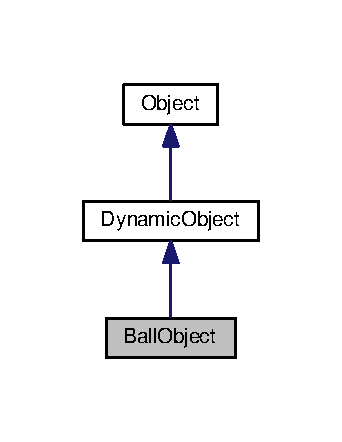
\includegraphics[width=164pt]{classBallObject__inherit__graph}
\end{center}
\end{figure}


Collaboration diagram for Ball\+Object\+:
\nopagebreak
\begin{figure}[H]
\begin{center}
\leavevmode
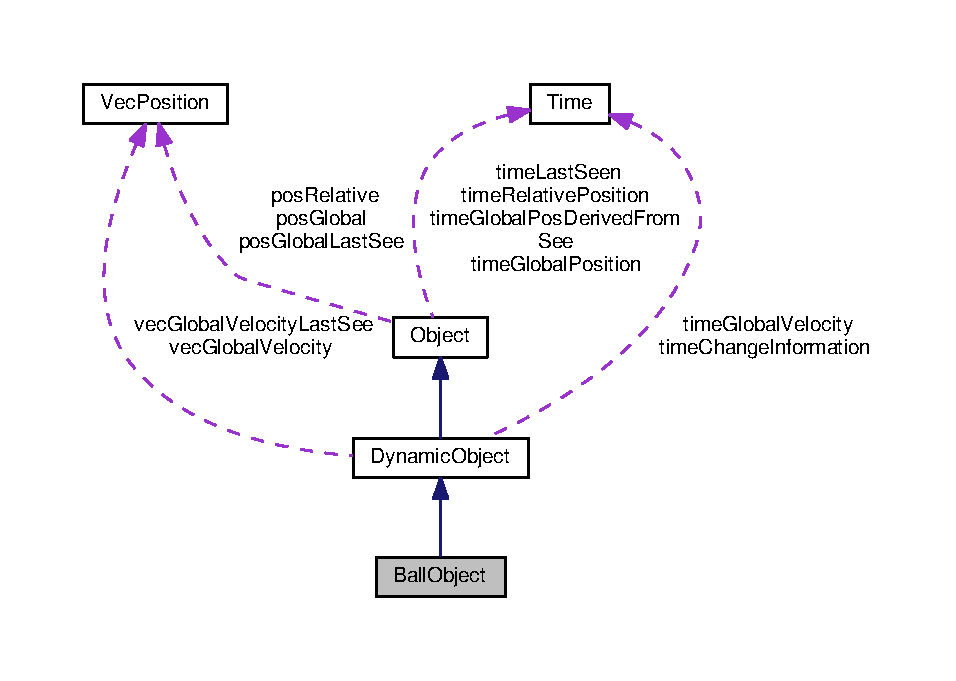
\includegraphics[width=350pt]{classBallObject__coll__graph}
\end{center}
\end{figure}
\subsection*{Public Member Functions}
\begin{DoxyCompactItemize}
\item 
\hyperlink{classBallObject_ac2106a42734e5028b3be1a38e8c39e31}{Ball\+Object} ()
\item 
void \hyperlink{classBallObject_a294d8fb34c88d98a1ef2ed2d1c864a62}{show} (ostream \&os=cout)
\end{DoxyCompactItemize}
\subsection*{Additional Inherited Members}


\subsection{Detailed Description}
Class \hyperlink{classPlayerObject}{Player\+Object} contains Robo\+Cup information that is available for the ball. No extra variables are added to superclass \hyperlink{classDynamicObject}{Dynamic\+Object} 

\subsection{Constructor \& Destructor Documentation}
\index{Ball\+Object@{Ball\+Object}!Ball\+Object@{Ball\+Object}}
\index{Ball\+Object@{Ball\+Object}!Ball\+Object@{Ball\+Object}}
\subsubsection[{\texorpdfstring{Ball\+Object()}{BallObject()}}]{\setlength{\rightskip}{0pt plus 5cm}Ball\+Object\+::\+Ball\+Object (
\begin{DoxyParamCaption}
{}
\end{DoxyParamCaption}
)}\hypertarget{classBallObject_ac2106a42734e5028b3be1a38e8c39e31}{}\label{classBallObject_ac2106a42734e5028b3be1a38e8c39e31}
This is the constructor for a \hyperlink{classBallObject}{Ball\+Object}. It does nothing except initializing the class. 

\subsection{Member Function Documentation}
\index{Ball\+Object@{Ball\+Object}!show@{show}}
\index{show@{show}!Ball\+Object@{Ball\+Object}}
\subsubsection[{\texorpdfstring{show(ostream \&os=cout)}{show(ostream &os=cout)}}]{\setlength{\rightskip}{0pt plus 5cm}void Ball\+Object\+::show (
\begin{DoxyParamCaption}
\item[{ostream \&}]{os = {\ttfamily cout}}
\end{DoxyParamCaption}
)\hspace{0.3cm}{\ttfamily [virtual]}}\hypertarget{classBallObject_a294d8fb34c88d98a1ef2ed2d1c864a62}{}\label{classBallObject_a294d8fb34c88d98a1ef2ed2d1c864a62}
This method prints information about the ball to the specified output stream


\begin{DoxyParams}{Parameters}
{\em os} & output stream to which information is written. \\
\hline
\end{DoxyParams}


Implements \hyperlink{classObject_abdfad2372e7ec5f9aa271a1677653778}{Object}.



The documentation for this class was generated from the following files\+:\begin{DoxyCompactItemize}
\item 
src/\hyperlink{Objects_8h}{Objects.\+h}\item 
src/\hyperlink{Objects_8cpp}{Objects.\+cpp}\end{DoxyCompactItemize}

\hypertarget{classBasicCoach}{}\section{Basic\+Coach Class Reference}
\label{classBasicCoach}\index{Basic\+Coach@{Basic\+Coach}}


{\ttfamily \#include $<$Basic\+Coach.\+h$>$}



Collaboration diagram for Basic\+Coach\+:
\nopagebreak
\begin{figure}[H]
\begin{center}
\leavevmode
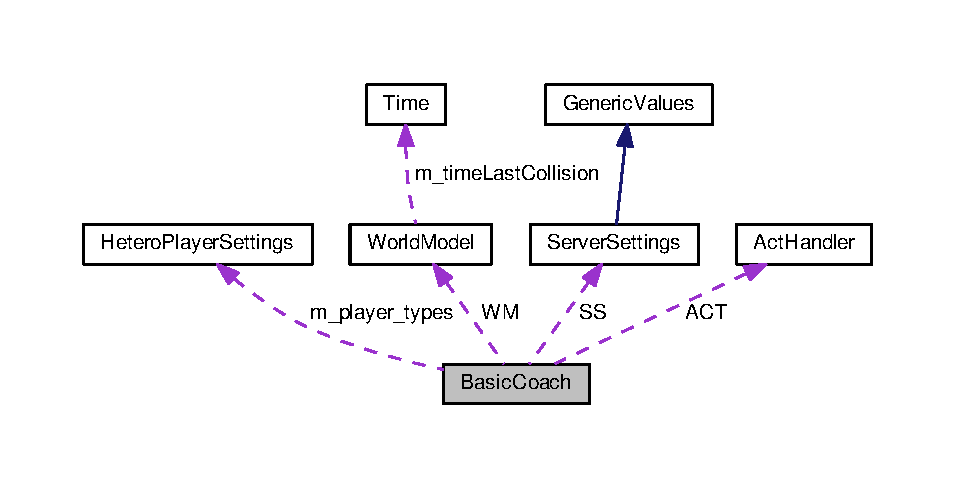
\includegraphics[width=350pt]{classBasicCoach__coll__graph}
\end{center}
\end{figure}
\subsection*{Public Member Functions}
\begin{DoxyCompactItemize}
\item 
\hyperlink{classBasicCoach_ad4034e11057d7502e4c3aa1ce8cb2aef}{Basic\+Coach} (\hyperlink{classActHandler}{Act\+Handler} $\ast$a, \hyperlink{classWorldModel}{World\+Model} $\ast$wm, \hyperlink{classServerSettings}{Server\+Settings} $\ast$ss, char $\ast$str\+Team\+Name, double d\+Version, bool is\+Trainer)
\item 
virtual void \hyperlink{classBasicCoach_a1f95a359aab679208c7fd00b0813fd52}{main\+Loop\+Normal} ()
\item 
void \hyperlink{classBasicCoach_a80c03fa2905d1e4024cfb9f3b6318e03}{substitute\+Player} (int i\+Player, int i\+Player\+Type)
\item 
void \hyperlink{classBasicCoach_a5508f69d366a39987d3c44aacdb25de9}{handle\+Stdin} ()
\item 
void \hyperlink{classBasicCoach_a67db9219b8bf738321c0eec0d738d3c7}{show\+String\+Commands} (ostream \&out)
\item 
bool \hyperlink{classBasicCoach_aaecc3faa1de4f37ca005040b397b9c9c}{execute\+String\+Command} (char $\ast$str)
\end{DoxyCompactItemize}
\subsection*{Protected Attributes}
\begin{DoxyCompactItemize}
\item 
\hyperlink{classActHandler}{Act\+Handler} $\ast$ \hyperlink{classBasicCoach_a3bbce5d14f0ceb04618a08c8005158fc}{A\+CT}
\item 
\hyperlink{classWorldModel}{World\+Model} $\ast$ \hyperlink{classBasicCoach_a82f305b964424a2200e875a73871c7fa}{WM}
\item 
\hyperlink{classServerSettings}{Server\+Settings} $\ast$ \hyperlink{classBasicCoach_acdde95fc653803caad2630b8d2f9026e}{SS}
\item 
\hyperlink{classHeteroPlayerSettings}{Hetero\+Player\+Settings} {\bfseries m\+\_\+player\+\_\+types} \mbox{[}\hyperlink{SoccerTypes_8h_ad5c84ed18f3f85d913cee3d8279b8879}{M\+A\+X\+\_\+\+H\+E\+T\+E\+R\+O\+\_\+\+P\+L\+A\+Y\+E\+RS}\mbox{]}\hypertarget{classBasicCoach_aca59e803723c90a74ffb76566fd31bf0}{}\label{classBasicCoach_aca59e803723c90a74ffb76566fd31bf0}

\item 
bool \hyperlink{classBasicCoach_a0d14913a2364960fdc647dbad35dd71d}{b\+Cont\+Loop}
\end{DoxyCompactItemize}


\subsection{Detailed Description}
This class starts a simple coach, which actions are defined in the method main\+Loop. It uses an \hyperlink{classActHandler}{Act\+Handler} to send actions to the server and can receive information from the \hyperlink{classWorldModel}{World\+Model}. The declaration of the different methods are defined in Basic\+Coach\+Test.\+C and Basic\+Coach.\+C. 

\subsection{Constructor \& Destructor Documentation}
\index{Basic\+Coach@{Basic\+Coach}!Basic\+Coach@{Basic\+Coach}}
\index{Basic\+Coach@{Basic\+Coach}!Basic\+Coach@{Basic\+Coach}}
\subsubsection[{\texorpdfstring{Basic\+Coach(\+Act\+Handler $\ast$a, World\+Model $\ast$wm, Server\+Settings $\ast$ss, char $\ast$str\+Team\+Name, double d\+Version, bool is\+Trainer)}{BasicCoach(ActHandler *a, WorldModel *wm, ServerSettings *ss, char *strTeamName, double dVersion, bool isTrainer)}}]{\setlength{\rightskip}{0pt plus 5cm}Basic\+Coach\+::\+Basic\+Coach (
\begin{DoxyParamCaption}
\item[{{\bf Act\+Handler} $\ast$}]{act, }
\item[{{\bf World\+Model} $\ast$}]{wm, }
\item[{{\bf Server\+Settings} $\ast$}]{ss, }
\item[{char $\ast$}]{str\+Team\+Name, }
\item[{double}]{d\+Version, }
\item[{bool}]{is\+Trainer}
\end{DoxyParamCaption}
)}\hypertarget{classBasicCoach_ad4034e11057d7502e4c3aa1ce8cb2aef}{}\label{classBasicCoach_ad4034e11057d7502e4c3aa1ce8cb2aef}
This is the constructor for the \hyperlink{classBasicCoach}{Basic\+Coach} class and contains the arguments that are used to initialize a coach. 
\begin{DoxyParams}{Parameters}
{\em act} & \hyperlink{classActHandler}{Act\+Handler} to which the actions can be sent \\
\hline
{\em wm} & \hyperlink{classWorldModel}{World\+Model} which information is used to determine action \\
\hline
{\em ss} & \hyperlink{classServerSettings}{Server\+Settings} that contain parameters used by the server \\
\hline
{\em str\+Team\+Name} & team name of this player \\
\hline
{\em d\+Version} & version this basiccoach corresponds to \\
\hline
{\em is\+Trainer} & indicates whether the coach is a trainer (offline coach) or an online coach (used during the match). \\
\hline
\end{DoxyParams}


\subsection{Member Function Documentation}
\index{Basic\+Coach@{Basic\+Coach}!execute\+String\+Command@{execute\+String\+Command}}
\index{execute\+String\+Command@{execute\+String\+Command}!Basic\+Coach@{Basic\+Coach}}
\subsubsection[{\texorpdfstring{execute\+String\+Command(char $\ast$str)}{executeStringCommand(char *str)}}]{\setlength{\rightskip}{0pt plus 5cm}bool Basic\+Coach\+::execute\+String\+Command (
\begin{DoxyParamCaption}
\item[{char $\ast$}]{str}
\end{DoxyParamCaption}
)}\hypertarget{classBasicCoach_aaecc3faa1de4f37ca005040b397b9c9c}{}\label{classBasicCoach_aaecc3faa1de4f37ca005040b397b9c9c}
This method executes the command that is entered by the user. For the possible command look at the method show\+String\+Commands. 
\begin{DoxyParams}{Parameters}
{\em str} & string that is entered by the user \\
\hline
\end{DoxyParams}
\begin{DoxyReturn}{Returns}
true when command could be executed, false otherwise 
\end{DoxyReturn}
\index{Basic\+Coach@{Basic\+Coach}!handle\+Stdin@{handle\+Stdin}}
\index{handle\+Stdin@{handle\+Stdin}!Basic\+Coach@{Basic\+Coach}}
\subsubsection[{\texorpdfstring{handle\+Stdin()}{handleStdin()}}]{\setlength{\rightskip}{0pt plus 5cm}void Basic\+Coach\+::handle\+Stdin (
\begin{DoxyParamCaption}
{}
\end{DoxyParamCaption}
)}\hypertarget{classBasicCoach_a5508f69d366a39987d3c44aacdb25de9}{}\label{classBasicCoach_a5508f69d366a39987d3c44aacdb25de9}
This method listens for input from the keyboard and when it receives this input it converts this input to the associated action. See show\+String\+Commands for the possible options. This method is used together with the \hyperlink{classSenseHandler}{Sense\+Handler} class that sends an alarm to indicate that a new command can be sent. This conflicts with the method in this method that listens for the user input (fgets) on Linux systems (on Solaris this isn\textquotesingle{}t a problem). The only known method is to use the flag S\+A\+\_\+\+R\+E\+S\+T\+A\+RT with this alarm function, but that does not seem to work under Linux. If each time the alarm is sent, this gets function unblocks, it will cause major performance problems. This function should not be called when a whole match is played! \index{Basic\+Coach@{Basic\+Coach}!main\+Loop\+Normal@{main\+Loop\+Normal}}
\index{main\+Loop\+Normal@{main\+Loop\+Normal}!Basic\+Coach@{Basic\+Coach}}
\subsubsection[{\texorpdfstring{main\+Loop\+Normal()}{mainLoopNormal()}}]{\setlength{\rightskip}{0pt plus 5cm}void Basic\+Coach\+::main\+Loop\+Normal (
\begin{DoxyParamCaption}
{}
\end{DoxyParamCaption}
)\hspace{0.3cm}{\ttfamily [virtual]}}\hypertarget{classBasicCoach_a1f95a359aab679208c7fd00b0813fd52}{}\label{classBasicCoach_a1f95a359aab679208c7fd00b0813fd52}
This method is the main loop of the coach. All sequence of actions are located in this method. \index{Basic\+Coach@{Basic\+Coach}!show\+String\+Commands@{show\+String\+Commands}}
\index{show\+String\+Commands@{show\+String\+Commands}!Basic\+Coach@{Basic\+Coach}}
\subsubsection[{\texorpdfstring{show\+String\+Commands(ostream \&out)}{showStringCommands(ostream &out)}}]{\setlength{\rightskip}{0pt plus 5cm}void Basic\+Coach\+::show\+String\+Commands (
\begin{DoxyParamCaption}
\item[{ostream \&}]{out}
\end{DoxyParamCaption}
)}\hypertarget{classBasicCoach_a67db9219b8bf738321c0eec0d738d3c7}{}\label{classBasicCoach_a67db9219b8bf738321c0eec0d738d3c7}
This method prints the possible commands that can be entered by the user. The whole name can be entered to perform the corresponding command, but normally only the first character is sufficient. This is indicated by putting brackets around the part of the command that is not needed. 
\begin{DoxyParams}{Parameters}
{\em out} & output stream to which the possible commands are printed \\
\hline
\end{DoxyParams}
\index{Basic\+Coach@{Basic\+Coach}!substitute\+Player@{substitute\+Player}}
\index{substitute\+Player@{substitute\+Player}!Basic\+Coach@{Basic\+Coach}}
\subsubsection[{\texorpdfstring{substitute\+Player(int i\+Player, int i\+Player\+Type)}{substitutePlayer(int iPlayer, int iPlayerType)}}]{\setlength{\rightskip}{0pt plus 5cm}void Basic\+Coach\+::substitute\+Player (
\begin{DoxyParamCaption}
\item[{int}]{i\+Player, }
\item[{int}]{i\+Player\+Type}
\end{DoxyParamCaption}
)}\hypertarget{classBasicCoach_a80c03fa2905d1e4024cfb9f3b6318e03}{}\label{classBasicCoach_a80c03fa2905d1e4024cfb9f3b6318e03}
This method substitutes one player to the given player type and sends this command (using the \hyperlink{classActHandler}{Act\+Handler}) to the soccer server. 

\subsection{Member Data Documentation}
\index{Basic\+Coach@{Basic\+Coach}!A\+CT@{A\+CT}}
\index{A\+CT@{A\+CT}!Basic\+Coach@{Basic\+Coach}}
\subsubsection[{\texorpdfstring{A\+CT}{ACT}}]{\setlength{\rightskip}{0pt plus 5cm}{\bf Act\+Handler}$\ast$ Basic\+Coach\+::\+A\+CT\hspace{0.3cm}{\ttfamily [protected]}}\hypertarget{classBasicCoach_a3bbce5d14f0ceb04618a08c8005158fc}{}\label{classBasicCoach_a3bbce5d14f0ceb04618a08c8005158fc}
\hyperlink{classActHandler}{Act\+Handler} to which commands can be sent \index{Basic\+Coach@{Basic\+Coach}!b\+Cont\+Loop@{b\+Cont\+Loop}}
\index{b\+Cont\+Loop@{b\+Cont\+Loop}!Basic\+Coach@{Basic\+Coach}}
\subsubsection[{\texorpdfstring{b\+Cont\+Loop}{bContLoop}}]{\setlength{\rightskip}{0pt plus 5cm}bool Basic\+Coach\+::b\+Cont\+Loop\hspace{0.3cm}{\ttfamily [protected]}}\hypertarget{classBasicCoach_a0d14913a2364960fdc647dbad35dd71d}{}\label{classBasicCoach_a0d14913a2364960fdc647dbad35dd71d}
bool to indicate whether to stop or continue \index{Basic\+Coach@{Basic\+Coach}!SS@{SS}}
\index{SS@{SS}!Basic\+Coach@{Basic\+Coach}}
\subsubsection[{\texorpdfstring{SS}{SS}}]{\setlength{\rightskip}{0pt plus 5cm}{\bf Server\+Settings}$\ast$ Basic\+Coach\+::\+SS\hspace{0.3cm}{\ttfamily [protected]}}\hypertarget{classBasicCoach_acdde95fc653803caad2630b8d2f9026e}{}\label{classBasicCoach_acdde95fc653803caad2630b8d2f9026e}
All parameters used by the server \index{Basic\+Coach@{Basic\+Coach}!WM@{WM}}
\index{WM@{WM}!Basic\+Coach@{Basic\+Coach}}
\subsubsection[{\texorpdfstring{WM}{WM}}]{\setlength{\rightskip}{0pt plus 5cm}{\bf World\+Model}$\ast$ Basic\+Coach\+::\+WM\hspace{0.3cm}{\ttfamily [protected]}}\hypertarget{classBasicCoach_a82f305b964424a2200e875a73871c7fa}{}\label{classBasicCoach_a82f305b964424a2200e875a73871c7fa}
\hyperlink{classWorldModel}{World\+Model} that contains information of world 

The documentation for this class was generated from the following files\+:\begin{DoxyCompactItemize}
\item 
src/\hyperlink{BasicCoach_8h}{Basic\+Coach.\+h}\item 
src/\hyperlink{BasicCoach_8cpp}{Basic\+Coach.\+cpp}\end{DoxyCompactItemize}

\hypertarget{classBasicPlayer}{}\section{Basic\+Player Class Reference}
\label{classBasicPlayer}\index{Basic\+Player@{Basic\+Player}}


{\ttfamily \#include $<$Basic\+Player.\+h$>$}



Inheritance diagram for Basic\+Player\+:
\nopagebreak
\begin{figure}[H]
\begin{center}
\leavevmode
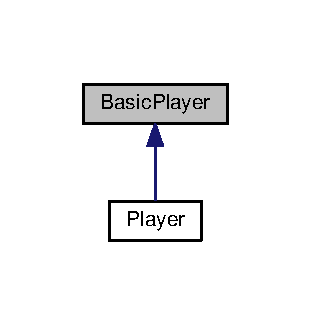
\includegraphics[width=149pt]{classBasicPlayer__inherit__graph}
\end{center}
\end{figure}


Collaboration diagram for Basic\+Player\+:
\nopagebreak
\begin{figure}[H]
\begin{center}
\leavevmode
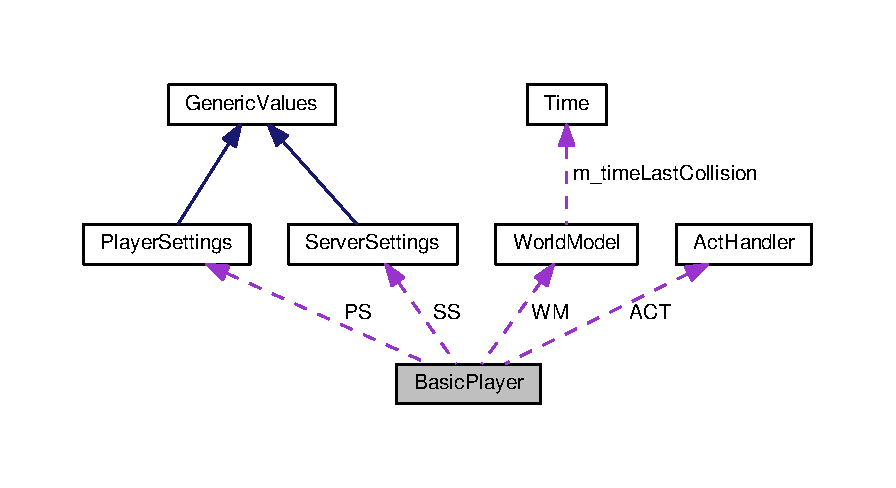
\includegraphics[width=350pt]{classBasicPlayer__coll__graph}
\end{center}
\end{figure}
\subsection*{Protected Member Functions}
\begin{DoxyCompactItemize}
\item 
\hyperlink{classSoccerCommand}{Soccer\+Command} \hyperlink{classBasicPlayer_a8110d9253af12626e3a404cfe476bed0}{align\+Neck\+With\+Body} ()
\item 
\hyperlink{classSoccerCommand}{Soccer\+Command} \hyperlink{classBasicPlayer_a4f4762b6f8a9938bd5142bee0865a72e}{turn\+Body\+To\+Point} (\hyperlink{classVecPosition}{Vec\+Position} pos, int i\+Pos=1)
\item 
\hyperlink{classSoccerCommand}{Soccer\+Command} \hyperlink{classBasicPlayer_acb667ad61ced5f4fea1b6552d7a218ca}{turn\+Back\+To\+Point} (\hyperlink{classVecPosition}{Vec\+Position} pos, int i\+Pos=1)
\item 
\hyperlink{classSoccerCommand}{Soccer\+Command} {\bfseries turn\+Side\+To\+Point} (\hyperlink{classVecPosition}{Vec\+Position} pos, \hyperlink{Geometry_8h_a6bfe02ae9bb185092902092561ab2865}{Ang\+Deg} angle, int i\+Cycles=1)\hypertarget{classBasicPlayer_abdeb44dc297eae5ea895a3adc1f40c44}{}\label{classBasicPlayer_abdeb44dc297eae5ea895a3adc1f40c44}

\item 
\hyperlink{classSoccerCommand}{Soccer\+Command} \hyperlink{classBasicPlayer_a651d2599323445ef450bd9af94c5c7ca}{turn\+Neck\+To\+Point} (\hyperlink{classVecPosition}{Vec\+Position} pos, \hyperlink{classSoccerCommand}{Soccer\+Command} com)
\item 
\hyperlink{classSoccerCommand}{Soccer\+Command} \hyperlink{classBasicPlayer_ad9700140b78ffeb1794366cf63836e21}{search\+Ball} ()
\item 
\hyperlink{classSoccerCommand}{Soccer\+Command} \hyperlink{classBasicPlayer_af7da70e5ce312ed3e4365531f050195f}{dash\+To\+Point} (\hyperlink{classVecPosition}{Vec\+Position} pos, int i\+Cycles=1, bool side\+Dash=false)
\item 
\hyperlink{classSoccerCommand}{Soccer\+Command} \hyperlink{classBasicPlayer_a6edbb52467b3952693bc5e86d6230473}{freeze\+Ball} ()
\item 
\hyperlink{classSoccerCommand}{Soccer\+Command} \hyperlink{classBasicPlayer_a517b7d4ef489a3476662939019e1d66d}{kick\+Ball\+Close\+To\+Body} (\hyperlink{Geometry_8h_a6bfe02ae9bb185092902092561ab2865}{Ang\+Deg} ang, double d\+Kick\+Ratio=0.\+16)
\item 
\hyperlink{classSoccerCommand}{Soccer\+Command} \hyperlink{classBasicPlayer_a3ebbd9fae54ebdca287d1c7aa2ce8b25}{accelerate\+Ball\+To\+Velocity} (\hyperlink{classVecPosition}{Vec\+Position} vel)
\item 
\hyperlink{classSoccerCommand}{Soccer\+Command} \hyperlink{classBasicPlayer_a61de8901846464425f2670dc4f976ab0}{catch\+Ball} ()
\item 
\hyperlink{classSoccerCommand}{Soccer\+Command} \hyperlink{classBasicPlayer_a22df9c1f41ddd210ffc6d97e56a2b904}{communicate} (char $\ast$str)
\item 
\hyperlink{classSoccerCommand}{Soccer\+Command} \hyperlink{classBasicPlayer_a22ffa701a6b2da41c70b60a8c244d96d}{teleport\+To\+Pos} (\hyperlink{classVecPosition}{Vec\+Position} pos)
\item 
\hyperlink{classSoccerCommand}{Soccer\+Command} \hyperlink{classBasicPlayer_a4e9844c2ef6e7c53c604835c9423638a}{listen\+To} (\hyperlink{SoccerTypes_8h_ad4b701fa66e7d26c054ed15b7820c77c}{ObjectT} obj)
\item 
\hyperlink{classSoccerCommand}{Soccer\+Command} \hyperlink{classBasicPlayer_a987d8442964607644adf5bcd539a0659}{tackle} (double power\+Or\+Angle)
\item 
\hyperlink{classSoccerCommand}{Soccer\+Command} \hyperlink{classBasicPlayer_a9374629af78e897891ab992a21f85f2a}{turn\+Body\+To\+Object} (\hyperlink{SoccerTypes_8h_ad4b701fa66e7d26c054ed15b7820c77c}{ObjectT} o)
\item 
\hyperlink{classSoccerCommand}{Soccer\+Command} \hyperlink{classBasicPlayer_aaf8a6bc96a2cafcf33fd2f4daabc1de0}{turn\+Neck\+To\+Object} (\hyperlink{SoccerTypes_8h_ad4b701fa66e7d26c054ed15b7820c77c}{ObjectT} o, \hyperlink{classSoccerCommand}{Soccer\+Command} com)
\item 
\hyperlink{classSoccerCommand}{Soccer\+Command} {\bfseries direct\+Towards} (\hyperlink{classVecPosition}{Vec\+Position} pos\+To, \hyperlink{Geometry_8h_a6bfe02ae9bb185092902092561ab2865}{Ang\+Deg} ang\+When\+To\+Turn, \hyperlink{classVecPosition}{Vec\+Position} $\ast$pos=N\+U\+LL, \hyperlink{classVecPosition}{Vec\+Position} $\ast$vel=N\+U\+LL, \hyperlink{Geometry_8h_a6bfe02ae9bb185092902092561ab2865}{Ang\+Deg} $\ast$ang\+Body=N\+U\+LL)\hypertarget{classBasicPlayer_a393a33539a9af09838e90c58428572cf}{}\label{classBasicPlayer_a393a33539a9af09838e90c58428572cf}

\item 
\hyperlink{classSoccerCommand}{Soccer\+Command} \hyperlink{classBasicPlayer_a0310219cd313d63785a72d482db2348b}{move\+To\+Pos} (\hyperlink{classVecPosition}{Vec\+Position} pos\+To, \hyperlink{Geometry_8h_a6bfe02ae9bb185092902092561ab2865}{Ang\+Deg} ang\+When\+To\+Turn, double d\+Dist\+Dash\+Back=0.\+0, bool b\+Move\+Back=false, int i\+Cycles=1)
\item 
\hyperlink{classSoccerCommand}{Soccer\+Command} \hyperlink{classBasicPlayer_a69ab617e6e772c686efec2d94d780723}{move\+To\+Pos2} (\hyperlink{classVecPosition}{Vec\+Position} pos\+To, \hyperlink{Geometry_8h_a6bfe02ae9bb185092902092561ab2865}{Ang\+Deg} ang\+When\+To\+Turn, double angle)
\item 
\hyperlink{classSoccerCommand}{Soccer\+Command} \hyperlink{classBasicPlayer_aac84d06304774170af7b01162558da3e}{collide\+With\+Ball} ()
\item 
\hyperlink{classSoccerCommand}{Soccer\+Command} \hyperlink{classBasicPlayer_abcee3b0e4dadf0305022280beaf5991e}{intercept\+Close} ()
\item 
\hyperlink{classSoccerCommand}{Soccer\+Command} \hyperlink{classBasicPlayer_a93a7e41c8b11d8fe6b92f950141a6ec3}{intercept\+Close\+Goalie} ()
\item 
\hyperlink{classSoccerCommand}{Soccer\+Command} \hyperlink{classBasicPlayer_a502eaf4aa2a5ba85af56f6863e767395}{kick\+To} (\hyperlink{classVecPosition}{Vec\+Position} pos\+Target, double d\+End\+Speed)
\item 
\hyperlink{classSoccerCommand}{Soccer\+Command} \hyperlink{classBasicPlayer_a6b8241babfa3f51132484b2ff73af042}{turn\+With\+Ball\+To} (\hyperlink{Geometry_8h_a6bfe02ae9bb185092902092561ab2865}{Ang\+Deg} ang, \hyperlink{Geometry_8h_a6bfe02ae9bb185092902092561ab2865}{Ang\+Deg} ang\+Kick\+Thr, double d\+Freeze\+Thr)
\item 
\hyperlink{classSoccerCommand}{Soccer\+Command} \hyperlink{classBasicPlayer_a05e0fa368dc255e0d36c5d4b72d23899}{move\+To\+Pos\+Along\+Line} (\hyperlink{classVecPosition}{Vec\+Position} pos, \hyperlink{Geometry_8h_a6bfe02ae9bb185092902092561ab2865}{Ang\+Deg} ang, double d\+Dist\+Thr, int i\+Sign, \hyperlink{Geometry_8h_a6bfe02ae9bb185092902092561ab2865}{Ang\+Deg} ang\+Thr, \hyperlink{Geometry_8h_a6bfe02ae9bb185092902092561ab2865}{Ang\+Deg} ang\+Corr)
\item 
\hyperlink{classSoccerCommand}{Soccer\+Command} \hyperlink{classBasicPlayer_af6b9642a2abd6f5f3fc359589d1373d6}{intercept} (bool is\+Goalie)
\item 
\hyperlink{classSoccerCommand}{Soccer\+Command} \hyperlink{classBasicPlayer_a63e33779fbadff1b61a499c4176ac6f4}{dribble} (\hyperlink{Geometry_8h_a6bfe02ae9bb185092902092561ab2865}{Ang\+Deg} ang, \hyperlink{SoccerTypes_8h_a0ccbf575eb8292e31644ccf3e84e3e3b}{DribbleT} d)
\item 
\hyperlink{classSoccerCommand}{Soccer\+Command} \hyperlink{classBasicPlayer_a687cc07033c6546931971f570c1e3a67}{direct\+Pass} (\hyperlink{classVecPosition}{Vec\+Position} pos, \hyperlink{SoccerTypes_8h_ab93ab6e2460fd3f4ae01757ea619ee30}{PassT} pass\+Type)
\item 
\hyperlink{classSoccerCommand}{Soccer\+Command} \hyperlink{classBasicPlayer_a9c6793780826b51a126102c5d29707ea}{leading\+Pass} (\hyperlink{SoccerTypes_8h_ad4b701fa66e7d26c054ed15b7820c77c}{ObjectT} o, double d\+Dist, \hyperlink{SoccerTypes_8h_a8e832a4ec6c67d3151112ed1e1c67752}{DirectionT} dir=\hyperlink{SoccerTypes_8h_a8e832a4ec6c67d3151112ed1e1c67752a944af66843e2c071955de8dfc4e7f407}{D\+I\+R\+\_\+\+N\+O\+R\+TH})
\item 
\hyperlink{classSoccerCommand}{Soccer\+Command} \hyperlink{classBasicPlayer_aca8ea920641ef60220f1ff9ce4975268}{through\+Pass} (\hyperlink{SoccerTypes_8h_ad4b701fa66e7d26c054ed15b7820c77c}{ObjectT} o, \hyperlink{classVecPosition}{Vec\+Position} pos\+End, \hyperlink{Geometry_8h_a6bfe02ae9bb185092902092561ab2865}{Ang\+Deg} $\ast$ang\+Max=N\+U\+LL)
\item 
\hyperlink{classSoccerCommand}{Soccer\+Command} \hyperlink{classBasicPlayer_ae16c69a2f51d2eafd1e01ae6664059fe}{outplay\+Opponent} (\hyperlink{SoccerTypes_8h_ad4b701fa66e7d26c054ed15b7820c77c}{ObjectT} o, \hyperlink{classVecPosition}{Vec\+Position} pos, \hyperlink{classVecPosition}{Vec\+Position} $\ast$pos\+To=N\+U\+LL)
\item 
\hyperlink{classSoccerCommand}{Soccer\+Command} \hyperlink{classBasicPlayer_a06f048f249f2180bf287932724660a63}{clear\+Ball} (\hyperlink{SoccerTypes_8h_ae2955c91fd80f27b4c28cfd55a517e77}{Clear\+BallT} type, \hyperlink{SoccerTypes_8h_a8e9b8119c00121a197203aca01d5b090}{SideT} s=\hyperlink{SoccerTypes_8h_a8e9b8119c00121a197203aca01d5b090a15a5449d2724d5cf4a7855b32888b24a}{S\+I\+D\+E\+\_\+\+I\+L\+L\+E\+G\+AL}, \hyperlink{Geometry_8h_a6bfe02ae9bb185092902092561ab2865}{Ang\+Deg} $\ast$ang\+Max=N\+U\+LL)
\item 
\hyperlink{classSoccerCommand}{Soccer\+Command} \hyperlink{classBasicPlayer_ac5217a00d71206eaf17bf3656bd6f995}{mark} (\hyperlink{SoccerTypes_8h_ad4b701fa66e7d26c054ed15b7820c77c}{ObjectT} o, double d\+Dist, \hyperlink{SoccerTypes_8h_a4cc7adc5fa3df60a8143bd51fc421f92}{MarkT} mark)
\item 
\hyperlink{classSoccerCommand}{Soccer\+Command} \hyperlink{classBasicPlayer_ad6be860b141f47cb33eec9f0a3762dd8}{defend\+Goal\+Line} (double d\+Dist)
\item 
\hyperlink{classSoccerCommand}{Soccer\+Command} \hyperlink{classBasicPlayer_a20ea44e2d6f0105ae521c9ac9bf407ea}{intercept\+Scoring\+Attempt} ()
\item 
\hyperlink{classSoccerCommand}{Soccer\+Command} \hyperlink{classBasicPlayer_a6927be949526b68617b8663eae9e2b7d}{hold\+Ball} ()
\item 
\hyperlink{classVecPosition}{Vec\+Position} \hyperlink{classBasicPlayer_a803fc819ba92d02bf244d883f0f76203}{get\+Through\+Pass\+Shooting\+Point} (\hyperlink{SoccerTypes_8h_ad4b701fa66e7d26c054ed15b7820c77c}{ObjectT} obj\+Team, \hyperlink{classVecPosition}{Vec\+Position} pos\+End, \hyperlink{Geometry_8h_a6bfe02ae9bb185092902092561ab2865}{Ang\+Deg} $\ast$ang\+Max)
\item 
\hyperlink{classVecPosition}{Vec\+Position} \hyperlink{classBasicPlayer_af6cd1d09c374231ae78e10d0636a644d}{get\+Interception\+Point\+Ball} (int $\ast$i\+Cycles\+Ball, bool is\+Goalie)
\item 
\hyperlink{classVecPosition}{Vec\+Position} \hyperlink{classBasicPlayer_a1b50d5fb9c7fa0e5a90a7e4a215bafc0}{get\+Active\+Interception\+Point\+Ball} (int $\ast$i\+Cycles\+Ball, bool is\+Goalie)
\item 
\hyperlink{classVecPosition}{Vec\+Position} {\bfseries get\+Dribble\+Point} (\hyperlink{SoccerTypes_8h_a0ccbf575eb8292e31644ccf3e84e3e3b}{DribbleT} \hyperlink{classBasicPlayer_a63e33779fbadff1b61a499c4176ac6f4}{dribble}, double $\ast$d\+Dist)\hypertarget{classBasicPlayer_a9c4e9c5d0045117bc4ecfc75fc5b690c}{}\label{classBasicPlayer_a9c4e9c5d0045117bc4ecfc75fc5b690c}

\item 
\hyperlink{classVecPosition}{Vec\+Position} \hyperlink{classBasicPlayer_abf2b1236c259554ebdf96914ed2adb4f}{get\+Shoot\+Position\+On\+Line} (\hyperlink{classVecPosition}{Vec\+Position} p1, \hyperlink{classVecPosition}{Vec\+Position} p2, \hyperlink{Geometry_8h_a6bfe02ae9bb185092902092561ab2865}{Ang\+Deg} $\ast$ang\+Largest=N\+U\+LL)
\item 
double \hyperlink{classBasicPlayer_a95d6ecdb0d5f39f2644dc85e0da8cf3e}{get\+End\+Speed\+For\+Pass} (\hyperlink{SoccerTypes_8h_ad4b701fa66e7d26c054ed15b7820c77c}{ObjectT} o, \hyperlink{classVecPosition}{Vec\+Position} pos\+Pass)
\item 
\hyperlink{classVecPosition}{Vec\+Position} \hyperlink{classBasicPlayer_a914a86746493fefae4af754011b4150e}{get\+Marking\+Position} (\hyperlink{SoccerTypes_8h_ad4b701fa66e7d26c054ed15b7820c77c}{ObjectT} o, double d\+Dist, \hyperlink{SoccerTypes_8h_a4cc7adc5fa3df60a8143bd51fc421f92}{MarkT} \hyperlink{classBasicPlayer_ac5217a00d71206eaf17bf3656bd6f995}{mark})
\item 
double {\bfseries get\+Player\+Version} ()\hypertarget{classBasicPlayer_a05baabe77a35927934f2955deed50480}{}\label{classBasicPlayer_a05baabe77a35927934f2955deed50480}

\item 
\hyperlink{classSoccerCommand}{Soccer\+Command} {\bfseries sync\+See} ()\hypertarget{classBasicPlayer_aed979d279cb483bf8d5331d8cba0cd09}{}\label{classBasicPlayer_aed979d279cb483bf8d5331d8cba0cd09}

\end{DoxyCompactItemize}
\subsection*{Protected Attributes}
\begin{DoxyCompactItemize}
\item 
\hyperlink{classActHandler}{Act\+Handler} $\ast$ \hyperlink{classBasicPlayer_adb559ebfe52c2ca1b01cc21655bbed10}{A\+CT}
\item 
\hyperlink{classWorldModel}{World\+Model} $\ast$ \hyperlink{classBasicPlayer_a0a0a8b87ce4d8b6ad94a0fe594274715}{WM}
\item 
\hyperlink{classServerSettings}{Server\+Settings} $\ast$ \hyperlink{classBasicPlayer_a16daddc5f23e5862d115d1913a93fc1d}{SS}
\item 
\hyperlink{classPlayerSettings}{Player\+Settings} $\ast$ \hyperlink{classBasicPlayer_aef9a4fafd096a406d0ef5f85d11907b8}{PS}
\item 
double {\bfseries d\+Player\+Version}\hypertarget{classBasicPlayer_a9bd93798246ad9f9c0d7d544d7439488}{}\label{classBasicPlayer_a9bd93798246ad9f9c0d7d544d7439488}

\end{DoxyCompactItemize}


\subsection{Detailed Description}
This class defines the skills that can be used by an agent. No functionality is available that chooses when to execute which skill, this is done in the \hyperlink{classPlayer}{Player} class. The \hyperlink{classWorldModel}{World\+Model} is used to determine the way in which the skills are performed. 

\subsection{Member Function Documentation}
\index{Basic\+Player@{Basic\+Player}!accelerate\+Ball\+To\+Velocity@{accelerate\+Ball\+To\+Velocity}}
\index{accelerate\+Ball\+To\+Velocity@{accelerate\+Ball\+To\+Velocity}!Basic\+Player@{Basic\+Player}}
\subsubsection[{\texorpdfstring{accelerate\+Ball\+To\+Velocity(\+Vec\+Position vel)}{accelerateBallToVelocity(VecPosition vel)}}]{\setlength{\rightskip}{0pt plus 5cm}{\bf Soccer\+Command} Basic\+Player\+::accelerate\+Ball\+To\+Velocity (
\begin{DoxyParamCaption}
\item[{{\bf Vec\+Position}}]{vel\+Des}
\end{DoxyParamCaption}
)\hspace{0.3cm}{\ttfamily [protected]}}\hypertarget{classBasicPlayer_a3ebbd9fae54ebdca287d1c7aa2ce8b25}{}\label{classBasicPlayer_a3ebbd9fae54ebdca287d1c7aa2ce8b25}
This skill enables an agent to accelerate the ball in such a way that it gets a certain velocity after the kick. It receives the desired velocity \textquotesingle{}vec\+Des\textquotesingle{} as its only argument and returns a kick command that causes the ball to be accelerated to this velocity. If the power that must be supplied to the kick command to get the desired result does not exceed the maximum kick power then the desired velocity can be realized with a single kick. The kick direction should then be equal to the direction of the acceleration vector relative to the agent\textquotesingle{}s global body angle. However, if the desired velocity is too great or if the current ball velocity is too high then the required acceleration cannot be realized with a single kick. In this case, the ball is kicked in such a way that the acceleration vector has the maximum possible length and a direction that aligns the resulting ball movement with \textquotesingle{}vec\+Des\textquotesingle{}. This means that after the kick the ball will move in the same direction as \textquotesingle{}vec\+Des\textquotesingle{} but at a lower speed. To this end the acceleration vector has to compensate for the current ball velocity in the `wrong\textquotesingle{} direction (y-\/component). 
\begin{DoxyParams}{Parameters}
{\em vel\+Des} & desired ball velocity \\
\hline
\end{DoxyParams}
\begin{DoxyReturn}{Returns}
\hyperlink{classSoccerCommand}{Soccer\+Command} that accelerates the ball to \textquotesingle{}vec\+Des\textquotesingle{} 
\end{DoxyReturn}
\index{Basic\+Player@{Basic\+Player}!align\+Neck\+With\+Body@{align\+Neck\+With\+Body}}
\index{align\+Neck\+With\+Body@{align\+Neck\+With\+Body}!Basic\+Player@{Basic\+Player}}
\subsubsection[{\texorpdfstring{align\+Neck\+With\+Body()}{alignNeckWithBody()}}]{\setlength{\rightskip}{0pt plus 5cm}{\bf Soccer\+Command} Basic\+Player\+::align\+Neck\+With\+Body (
\begin{DoxyParamCaption}
{}
\end{DoxyParamCaption}
)\hspace{0.3cm}{\ttfamily [protected]}}\hypertarget{classBasicPlayer_a8110d9253af12626e3a404cfe476bed0}{}\label{classBasicPlayer_a8110d9253af12626e3a404cfe476bed0}
This skill enables an agent to align his neck with his body. It returns a turn neck command that takes the angle of the agent\textquotesingle{}s body relative to his neck as its only argument. \begin{DoxyReturn}{Returns}
\hyperlink{classSoccerCommand}{Soccer\+Command} turn\+\_\+neck command that aligns neck with body 
\end{DoxyReturn}
\index{Basic\+Player@{Basic\+Player}!catch\+Ball@{catch\+Ball}}
\index{catch\+Ball@{catch\+Ball}!Basic\+Player@{Basic\+Player}}
\subsubsection[{\texorpdfstring{catch\+Ball()}{catchBall()}}]{\setlength{\rightskip}{0pt plus 5cm}{\bf Soccer\+Command} Basic\+Player\+::catch\+Ball (
\begin{DoxyParamCaption}
{}
\end{DoxyParamCaption}
)\hspace{0.3cm}{\ttfamily [protected]}}\hypertarget{classBasicPlayer_a61de8901846464425f2670dc4f976ab0}{}\label{classBasicPlayer_a61de8901846464425f2670dc4f976ab0}
This skill enables an agent to catch the ball and can only be executed when the agent is a goalkeeper. It returns a catch command that takes the angle of the ball relative to the body of the agent as its only argument. The correct value for this argument is computed by determining the global direction between the current ball position and the agent\textquotesingle{}s current position and by making this direction relative to the agent\textquotesingle{}s global body angle. \begin{DoxyReturn}{Returns}
\hyperlink{classSoccerCommand}{Soccer\+Command} to catch the ball 
\end{DoxyReturn}
\index{Basic\+Player@{Basic\+Player}!clear\+Ball@{clear\+Ball}}
\index{clear\+Ball@{clear\+Ball}!Basic\+Player@{Basic\+Player}}
\subsubsection[{\texorpdfstring{clear\+Ball(\+Clear\+Ball\+T type, Side\+T s=\+S\+I\+D\+E\+\_\+\+I\+L\+L\+E\+G\+A\+L, Ang\+Deg $\ast$ang\+Max=\+N\+U\+L\+L)}{clearBall(ClearBallT type, SideT s=SIDE_ILLEGAL, AngDeg *angMax=NULL)}}]{\setlength{\rightskip}{0pt plus 5cm}{\bf Soccer\+Command} Basic\+Player\+::clear\+Ball (
\begin{DoxyParamCaption}
\item[{{\bf Clear\+BallT}}]{type, }
\item[{{\bf SideT}}]{s = {\ttfamily {\bf S\+I\+D\+E\+\_\+\+I\+L\+L\+E\+G\+AL}}, }
\item[{{\bf Ang\+Deg} $\ast$}]{ang\+Max = {\ttfamily NULL}}
\end{DoxyParamCaption}
)\hspace{0.3cm}{\ttfamily [protected]}}\hypertarget{classBasicPlayer_a06f048f249f2180bf287932724660a63}{}\label{classBasicPlayer_a06f048f249f2180bf287932724660a63}
This skill enables an agent to clear the ball to a certain area on the field. It is useful, for example, when a defender cannot dribble or pass the ball to a teammate in a dangerous situation. Using this skill he can then kick the ball up the field away from the defensive zone. It is important to realize that this skill is only called when the agent has no alternative options in the current situation. Clearing the ball amounts to kicking it with maximum power into the widest angle between opponents in a certain area. The shooting direction is determined using the function which returns the direction of the bisector of this widest angle. The area on the field from which this angle is selected depends on the type of clear which is supplied as an argument to this skill. We distinguish three types of clearing\+:
\begin{DoxyItemize}
\item C\+L\+E\+AR B\+A\+LL D\+E\+F\+E\+N\+S\+I\+VE\+: clearing the ball away from the defensive zone into a triangular area which is defined by the current ball position and the center line on the field.
\item C\+L\+E\+AR B\+A\+LL O\+F\+F\+E\+N\+S\+I\+VE\+: clearing the ball towards the offensive zone into a triangular area which is defined by the current ball position and the line segment that coincides with the front line of the opponent\textquotesingle{}s penalty area and extends to the left and right side lines.
\item C\+L\+E\+AR B\+A\+LL G\+O\+AL\+: clearing the ball into a triangular area in front of the opponent\textquotesingle{}s goal which is defined by the current ball position and the line segment that runs from the center of the opponent\textquotesingle{}s goal to the center of the front line of the penalty area. 
\begin{DoxyParams}{Parameters}
{\em type} & type of the clear ball skill \\
\hline
{\em s} & if specified indicates the part of the field the clear\+Ball should be directed to. \\
\hline
{\em ang\+Max} & if specified (and not N\+U\+LL) will be filled with the angle between the opponents in the direction in which will be shot \\
\hline
\end{DoxyParams}
\begin{DoxyReturn}{Returns}
\hyperlink{classSoccerCommand}{Soccer\+Command} kick command to clear the ball 
\end{DoxyReturn}

\end{DoxyItemize}\index{Basic\+Player@{Basic\+Player}!collide\+With\+Ball@{collide\+With\+Ball}}
\index{collide\+With\+Ball@{collide\+With\+Ball}!Basic\+Player@{Basic\+Player}}
\subsubsection[{\texorpdfstring{collide\+With\+Ball()}{collideWithBall()}}]{\setlength{\rightskip}{0pt plus 5cm}{\bf Soccer\+Command} Basic\+Player\+::collide\+With\+Ball (
\begin{DoxyParamCaption}
{}
\end{DoxyParamCaption}
)\hspace{0.3cm}{\ttfamily [protected]}}\hypertarget{classBasicPlayer_aac84d06304774170af7b01162558da3e}{}\label{classBasicPlayer_aac84d06304774170af7b01162558da3e}
This method returns a command that can be used to collide with the ball on purpose. When this is not possible. C\+M\+D\+\_\+\+I\+L\+L\+E\+G\+AL is returned. Colliding with the ball may be useful when the player is turned with his back to the opponent goal and is intercepting a moving ball, by colliding both the ball and the player will loose all their velocity. Now the player can turn at once to the desired direction. Otherwise he first has to freeze the ball, freeze his own speed and then turn around. \index{Basic\+Player@{Basic\+Player}!communicate@{communicate}}
\index{communicate@{communicate}!Basic\+Player@{Basic\+Player}}
\subsubsection[{\texorpdfstring{communicate(char $\ast$str)}{communicate(char *str)}}]{\setlength{\rightskip}{0pt plus 5cm}{\bf Soccer\+Command} Basic\+Player\+::communicate (
\begin{DoxyParamCaption}
\item[{char $\ast$}]{str}
\end{DoxyParamCaption}
)\hspace{0.3cm}{\ttfamily [protected]}}\hypertarget{classBasicPlayer_a22df9c1f41ddd210ffc6d97e56a2b904}{}\label{classBasicPlayer_a22df9c1f41ddd210ffc6d97e56a2b904}
This skill enables an agent to communicate with other players on the field. It receives a string message as its only argument and returns a say command that causes the message to be broadcast to all players within a certain distance from the speaker. \begin{DoxyReturn}{Returns}
\hyperlink{classSoccerCommand}{Soccer\+Command} to say the specified string \textquotesingle{}str\textquotesingle{} 
\end{DoxyReturn}
\index{Basic\+Player@{Basic\+Player}!dash\+To\+Point@{dash\+To\+Point}}
\index{dash\+To\+Point@{dash\+To\+Point}!Basic\+Player@{Basic\+Player}}
\subsubsection[{\texorpdfstring{dash\+To\+Point(\+Vec\+Position pos, int i\+Cycles=1, bool side\+Dash=false)}{dashToPoint(VecPosition pos, int iCycles=1, bool sideDash=false)}}]{\setlength{\rightskip}{0pt plus 5cm}{\bf Soccer\+Command} Basic\+Player\+::dash\+To\+Point (
\begin{DoxyParamCaption}
\item[{{\bf Vec\+Position}}]{pos, }
\item[{int}]{i\+Cycles = {\ttfamily 1}, }
\item[{bool}]{side\+Dash = {\ttfamily false}}
\end{DoxyParamCaption}
)\hspace{0.3cm}{\ttfamily [protected]}}\hypertarget{classBasicPlayer_af7da70e5ce312ed3e4365531f050195f}{}\label{classBasicPlayer_af7da70e5ce312ed3e4365531f050195f}
This method can be called to create a \hyperlink{classSoccerCommand}{Soccer\+Command} that dashes to a point. This skill enables an agent to dash to a given point. It receives a global position \textquotesingle{}pos\textquotesingle{} as its only argument and returns a dash command that causes the agent to come as close to this point as possible. Since the agent can only move forwards or backwards, the closest point to the target position that he can reach by dashing is the orthogonal projection of \textquotesingle{}pos\textquotesingle{} onto the line that extends into the direction of his body (forwards and backwards). The power that must be supplied to the dash command is computed using the \textquotesingle{}get\+Power\+For\+Dash\textquotesingle{} method which takes the position of \textquotesingle{}pos\textquotesingle{} relative to the agent as input and \textquotesingle{}i\+Cycles\textquotesingle{} which denotes in how many cycles we want to reach that point. 
\begin{DoxyParams}{Parameters}
{\em pos} & global position to which the agent wants to dash \\
\hline
{\em i\+Cycles} & desired number of cycles to reach point \textquotesingle{}pos\textquotesingle{} \\
\hline
\end{DoxyParams}
\begin{DoxyReturn}{Returns}
\hyperlink{classSoccerCommand}{Soccer\+Command} dash command to move closer to \textquotesingle{}pos\textquotesingle{} 
\end{DoxyReturn}
\index{Basic\+Player@{Basic\+Player}!defend\+Goal\+Line@{defend\+Goal\+Line}}
\index{defend\+Goal\+Line@{defend\+Goal\+Line}!Basic\+Player@{Basic\+Player}}
\subsubsection[{\texorpdfstring{defend\+Goal\+Line(double d\+Dist)}{defendGoalLine(double dDist)}}]{\setlength{\rightskip}{0pt plus 5cm}{\bf Soccer\+Command} Basic\+Player\+::defend\+Goal\+Line (
\begin{DoxyParamCaption}
\item[{double}]{d\+Dist}
\end{DoxyParamCaption}
)\hspace{0.3cm}{\ttfamily [protected]}}\hypertarget{classBasicPlayer_ad6be860b141f47cb33eec9f0a3762dd8}{}\label{classBasicPlayer_ad6be860b141f47cb33eec9f0a3762dd8}
This skill enables an agent (usually the goalkeeper) to defend his own goal line. To this end the agent moves to a position along a line l which runs parallel to the goal line at a small distance \textquotesingle{}d\+Dist\textquotesingle{} (supplied as an argument) from the goal. The guard point to which the agent moves depends on the predicted position of the ball in the next cycle and is chosen in anticipation of a future shot on goal. This means that the guard point is selected in such a way that it will be most difficult for the opponent team to pass the goalkeeper. To find this point we need to look at the angle that the ball makes with respect to the left and right goal posts and we need to determine which point on l covers this angle in the most optimal way, i.\+e. leaves an equal gap to the left and to the right of the goalkeeper. Let m be the line that goes through the center point of the goal line and through the predicted ball position in the next cycle. Since this line m bisects the above-\/mentioned angle, the optimal guard point on l can be computed by determining the intersection between l and m. Note that in our current implementation the goalkeeper always stays in front of the goal mouth to avoid leaving an open goal when the ball is passed to an opponent in the center of the penalty area. The computed guard point is therefore adjusted if it lies too far to the side . After computing the guard point the goalkeeper needs to move to this point while keeping sight of the ball. If the distance between the current goalkeeper position and the line l is larger than Defend\+Goal\+Line\+Max\+Dist (which has a value of 3.\+0 in our current implementation) the move\+To\+Pos skill is used to move directly towards the guard point. This can happen, for example, when the goalkeeper has moved forward from his line to intercept the ball and now has to move back to his line again. Note that the fourth argument supplied to the move\+To\+Pos skill equals true in this case to indicate that the goalkeeper wants to turn his back to the guard point in order to keep the ball in sight while moving. However, if the distance between the guard point and l is less than Defend\+Goal\+Line\+Max\+Dist then the move\+To\+Pos\+Along\+Line skill is used to move along l to the guard point. This skill receives an argument `sign\textquotesingle{} representing a prediction of the agent\textquotesingle{}s movement in the coming cycles. This value is used to adjust the agent\textquotesingle{}s body direction when necessary. In this case it can be expected that the goalkeeper will move along l in the same direction as the ball and `sign\textquotesingle{} is therefore determined by looking at the ball velocity in cycle t.


\begin{DoxyParams}{Parameters}
{\em d\+Dist} & distance before goal the goalkeeper will move along \\
\hline
\end{DoxyParams}
\begin{DoxyReturn}{Returns}
\hyperlink{classSoccerCommand}{Soccer\+Command} to defend the goal line. 
\end{DoxyReturn}
\index{Basic\+Player@{Basic\+Player}!direct\+Pass@{direct\+Pass}}
\index{direct\+Pass@{direct\+Pass}!Basic\+Player@{Basic\+Player}}
\subsubsection[{\texorpdfstring{direct\+Pass(\+Vec\+Position pos, Pass\+T pass\+Type)}{directPass(VecPosition pos, PassT passType)}}]{\setlength{\rightskip}{0pt plus 5cm}{\bf Soccer\+Command} Basic\+Player\+::direct\+Pass (
\begin{DoxyParamCaption}
\item[{{\bf Vec\+Position}}]{pos, }
\item[{{\bf PassT}}]{pass\+Type}
\end{DoxyParamCaption}
)\hspace{0.3cm}{\ttfamily [protected]}}\hypertarget{classBasicPlayer_a687cc07033c6546931971f570c1e3a67}{}\label{classBasicPlayer_a687cc07033c6546931971f570c1e3a67}
This skill enables an agent to pass the ball directly to another player. It receives two arguments, \textquotesingle{}pos\textquotesingle{} and \textquotesingle{}pass\+Type\textquotesingle{}, which respectively denote the position (of usually a teammate) to which the agent wants to pass the ball and the kind of pass (either normal or fast) that should be given. This skill uses the kick\+To skill to pass the ball to the specified position with a certain desired end speed depending on the type of pass. 
\begin{DoxyParams}{Parameters}
{\em pos} & position of object to which a direct pass should be given \\
\hline
{\em pass\+Type} & kind of pass (either P\+A\+S\+S\+\_\+\+N\+O\+R\+M\+AL or P\+A\+S\+S\+\_\+\+F\+A\+ST ) \\
\hline
\end{DoxyParams}
\begin{DoxyReturn}{Returns}
\hyperlink{classSoccerCommand}{Soccer\+Command} to perform a direct pass to object \textquotesingle{}o\textquotesingle{} 
\end{DoxyReturn}
\index{Basic\+Player@{Basic\+Player}!dribble@{dribble}}
\index{dribble@{dribble}!Basic\+Player@{Basic\+Player}}
\subsubsection[{\texorpdfstring{dribble(\+Ang\+Deg ang, Dribble\+T d)}{dribble(AngDeg ang, DribbleT d)}}]{\setlength{\rightskip}{0pt plus 5cm}{\bf Soccer\+Command} Basic\+Player\+::dribble (
\begin{DoxyParamCaption}
\item[{{\bf Ang\+Deg}}]{ang, }
\item[{{\bf DribbleT}}]{dribbleT}
\end{DoxyParamCaption}
)\hspace{0.3cm}{\ttfamily [protected]}}\hypertarget{classBasicPlayer_a63e33779fbadff1b61a499c4176ac6f4}{}\label{classBasicPlayer_a63e33779fbadff1b61a499c4176ac6f4}
This skill enables an agent to dribble with the ball, i.\+e. to move with the ball while keeping it within a certain distance. This amounts to repeatedly kicking the ball at a certain speed into a desired direction and then intercepting it again. Two arguments, the angle \textquotesingle{}ang\textquotesingle{} and type \textquotesingle{}dribbleT\textquotesingle{}, are supplied to this skill which respectively denote the global direction towards which the agent wants to dribble and the kind of dribble that must be performed. We distinguish three kinds of dribbling\+:
\begin{DoxyItemize}
\item D\+R\+I\+B\+B\+LE F\+A\+ST\+: a fast dribble action in which the agent kicks the ball relatively far ahead of him.
\item D\+R\+I\+B\+B\+LE S\+L\+OW\+: a slower dribble action in which the agent keeps the ball closer than on a fast dribble.
\item D\+R\+I\+B\+B\+LE W\+I\+TH B\+A\+LL\+: a safe dribble action in which the agent keeps the ball very close to his body.
\end{DoxyItemize}

It is important to realize that this skill is only called when the ball is located within the agent\textquotesingle{}s kickable range. This means that it is only responsible for the kicking part of the overall dribbling behavior, i.\+e. it only causes the ball to be kicked a certain distance ahead into the desired direction \textquotesingle{}ang\textquotesingle{}. If the absolute angle between \textquotesingle{}ang\textquotesingle{} and the agent\textquotesingle{}s body direction is larger than Dribble\+Turn\+Angle (which currently has a value of 30 degrees) then the agent uses the turn\+With\+Ball\+To skill to turn with the ball towards the global angle \textquotesingle{}ang\textquotesingle{}. Otherwise, he uses the kick\+To skill to kick the ball into the desired direction towards a point that lies a certain distance ahead depending on the type of dribble. After the kick, the ball will move out of the agent\textquotesingle{}s kickable range and as a result the agent will try to intercept it using the intercept skill. The dribbling skill can then be called again once the agent has succeeded in intercepting the ball. This sequence of kicking and intercepting will repeat itself until the agent decides to perform another skill. Note that during the dribble the power of a kick depends on the distance that the ball should travel and on the speed that it should have when it reaches the target point. In our current implementation this speed equals 0.\+5 (=Dribble\+Kick\+End\+Speed) for any type of dribble. Experiments have shown that lower end speed values cause the agent to intercept the ball before it reaches the target point which slows the dribble down significantly.


\begin{DoxyParams}{Parameters}
{\em ang} & global direction in which should be dribbled \\
\hline
{\em dribbleT} & type of dribble that should be performed \\
\hline
\end{DoxyParams}
\begin{DoxyReturn}{Returns}
\hyperlink{classSoccerCommand}{Soccer\+Command} to dribble in direction \textquotesingle{}ang\textquotesingle{} 
\end{DoxyReturn}
\index{Basic\+Player@{Basic\+Player}!freeze\+Ball@{freeze\+Ball}}
\index{freeze\+Ball@{freeze\+Ball}!Basic\+Player@{Basic\+Player}}
\subsubsection[{\texorpdfstring{freeze\+Ball()}{freezeBall()}}]{\setlength{\rightskip}{0pt plus 5cm}{\bf Soccer\+Command} Basic\+Player\+::freeze\+Ball (
\begin{DoxyParamCaption}
{}
\end{DoxyParamCaption}
)\hspace{0.3cm}{\ttfamily [protected]}}\hypertarget{classBasicPlayer_a6edbb52467b3952693bc5e86d6230473}{}\label{classBasicPlayer_a6edbb52467b3952693bc5e86d6230473}
This skill enables an agent to freeze a moving ball, i.\+e. it returns a kick command that stops the ball dead at its current position. Since ball movement in the soccer server is implemented as a vector addition, the ball will stop in the next cycle when it is kicked in such a way that the resulting acceleration vector has the same length and opposite direction to the current ball velocity. The desired speed that should be given to the ball on the kick thus equals the current ball speed. Furthermore, the direction of the kick should equal the direction of the current ball velocity plus 180 degrees. Note that this direction must be made relative to the agent\textquotesingle{}s global body angle before it can be passed as an argument to the kick command. \begin{DoxyReturn}{Returns}
\hyperlink{classSoccerCommand}{Soccer\+Command} to freeze the ball. 
\end{DoxyReturn}
\index{Basic\+Player@{Basic\+Player}!get\+Active\+Interception\+Point\+Ball@{get\+Active\+Interception\+Point\+Ball}}
\index{get\+Active\+Interception\+Point\+Ball@{get\+Active\+Interception\+Point\+Ball}!Basic\+Player@{Basic\+Player}}
\subsubsection[{\texorpdfstring{get\+Active\+Interception\+Point\+Ball(int $\ast$i\+Cycles\+Ball, bool is\+Goalie)}{getActiveInterceptionPointBall(int *iCyclesBall, bool isGoalie)}}]{\setlength{\rightskip}{0pt plus 5cm}{\bf Vec\+Position} Basic\+Player\+::get\+Active\+Interception\+Point\+Ball (
\begin{DoxyParamCaption}
\item[{int $\ast$}]{i\+Cycles\+Ball, }
\item[{bool}]{is\+Goalie}
\end{DoxyParamCaption}
)\hspace{0.3cm}{\ttfamily [protected]}}\hypertarget{classBasicPlayer_a1b50d5fb9c7fa0e5a90a7e4a215bafc0}{}\label{classBasicPlayer_a1b50d5fb9c7fa0e5a90a7e4a215bafc0}
This method intercepts the ball at the first possible position. 
\begin{DoxyParams}{Parameters}
{\em i\+Cycles\+Ball} & is the nr of cyles after the ball is intercepted \\
\hline
{\em is\+Goalie} & bool to indicate that a goalie has to intercept the ball \\
\hline
\end{DoxyParams}
\begin{DoxyReturn}{Returns}
intercept position 
\end{DoxyReturn}
\index{Basic\+Player@{Basic\+Player}!get\+End\+Speed\+For\+Pass@{get\+End\+Speed\+For\+Pass}}
\index{get\+End\+Speed\+For\+Pass@{get\+End\+Speed\+For\+Pass}!Basic\+Player@{Basic\+Player}}
\subsubsection[{\texorpdfstring{get\+End\+Speed\+For\+Pass(\+Object\+T o, Vec\+Position pos\+Pass)}{getEndSpeedForPass(ObjectT o, VecPosition posPass)}}]{\setlength{\rightskip}{0pt plus 5cm}double Basic\+Player\+::get\+End\+Speed\+For\+Pass (
\begin{DoxyParamCaption}
\item[{{\bf ObjectT}}]{o, }
\item[{{\bf Vec\+Position}}]{pos\+Pass}
\end{DoxyParamCaption}
)\hspace{0.3cm}{\ttfamily [protected]}}\hypertarget{classBasicPlayer_a95d6ecdb0d5f39f2644dc85e0da8cf3e}{}\label{classBasicPlayer_a95d6ecdb0d5f39f2644dc85e0da8cf3e}
This method returns the end speed for a pass. This end speed is determined using two parameters, \textquotesingle{}o\textquotesingle{} and \textquotesingle{}pos\+Pass\textquotesingle{} which respectively denote the object to which is passed and the position to which is passed. First it is determined how many server cycles \textquotesingle{}o\textquotesingle{} needs to travel to position \textquotesingle{}pos\+Pass\textquotesingle{}. Then the starting speed of the ball is determined when it wants to travel to \textquotesingle{}pos\+Pass\textquotesingle{} in the same number of cycles. This starting speed is adjusted if the corresponding end speed of the ball in the passing point lies outside the range \mbox{[}Min\+Pass\+End\+Speed .. Max\+Pass\+End\+Speed\mbox{]}. 
\begin{DoxyParams}{Parameters}
{\em o} & object to which the ball will be passed \\
\hline
{\em pos\+Pass} & desired passing point where o can intercept the ball \\
\hline
\end{DoxyParams}
\begin{DoxyReturn}{Returns}
end speed to give to the ball such that player can intercept the ball the best. 
\end{DoxyReturn}
\index{Basic\+Player@{Basic\+Player}!get\+Interception\+Point\+Ball@{get\+Interception\+Point\+Ball}}
\index{get\+Interception\+Point\+Ball@{get\+Interception\+Point\+Ball}!Basic\+Player@{Basic\+Player}}
\subsubsection[{\texorpdfstring{get\+Interception\+Point\+Ball(int $\ast$i\+Cycles\+Ball, bool is\+Goalie)}{getInterceptionPointBall(int *iCyclesBall, bool isGoalie)}}]{\setlength{\rightskip}{0pt plus 5cm}{\bf Vec\+Position} Basic\+Player\+::get\+Interception\+Point\+Ball (
\begin{DoxyParamCaption}
\item[{int $\ast$}]{i\+Min\+Cycles\+Ball, }
\item[{bool}]{is\+Goalie}
\end{DoxyParamCaption}
)\hspace{0.3cm}{\ttfamily [protected]}}\hypertarget{classBasicPlayer_af6cd1d09c374231ae78e10d0636a644d}{}\label{classBasicPlayer_af6cd1d09c374231ae78e10d0636a644d}
This method uses an iterative scheme to compute the optimal interception point of the ball. A loop is executed in which the prediction methods are used to predict the position of the ball a number of cycles, say i, into the future and to predict the number of cycles, say n, that the agent will need to reach this position. This is repeated for increasing values of i until n $<$ i in which case it is assumed thay the agent should be able to reach the predicted ball position before the ball does. This point is chosen as the interception point and the move\+To\+Pos skill is used to move towards this point.


\begin{DoxyParams}{Parameters}
{\em i\+Cycles\+To\+Ball} & will be filled with the nr of cycles it will take the ball to reach the returned position. \\
\hline
{\em is\+Goalie} & indicates whether the current player is a goalkeeper or not \\
\hline
\end{DoxyParams}
\begin{DoxyReturn}{Returns}
position to intercept the ball. 
\end{DoxyReturn}
\index{Basic\+Player@{Basic\+Player}!get\+Marking\+Position@{get\+Marking\+Position}}
\index{get\+Marking\+Position@{get\+Marking\+Position}!Basic\+Player@{Basic\+Player}}
\subsubsection[{\texorpdfstring{get\+Marking\+Position(\+Object\+T o, double d\+Dist, Mark\+T mark)}{getMarkingPosition(ObjectT o, double dDist, MarkT mark)}}]{\setlength{\rightskip}{0pt plus 5cm}{\bf Vec\+Position} Basic\+Player\+::get\+Marking\+Position (
\begin{DoxyParamCaption}
\item[{{\bf ObjectT}}]{o, }
\item[{double}]{d\+Dist, }
\item[{{\bf MarkT}}]{mark}
\end{DoxyParamCaption}
)\hspace{0.3cm}{\ttfamily [protected]}}\hypertarget{classBasicPlayer_a914a86746493fefae4af754011b4150e}{}\label{classBasicPlayer_a914a86746493fefae4af754011b4150e}
This method returns a global position on the field which denotes the position to mark object \textquotesingle{}o\textquotesingle{}. It receives three arguments\+: an object o (usually an opponent) that the agent wants to mark, a distance \textquotesingle{}d\+Dist\textquotesingle{} representing the desired distance between o and the marking position and a type indicator that denotes the type of marking that is required. We distinguish three types of marking\+:
\begin{DoxyItemize}
\item M\+A\+RK B\+A\+LL\+: marking the opponent by standing at a distance \textquotesingle{}d\+Dist\textquotesingle{} away from him on the line between him and the ball. This type of marking will make it di±cult for the opponent to receive a pass.
\item M\+A\+RK G\+O\+AL\+: marking the opponent by standing at a distance \textquotesingle{}d\+Dist\textquotesingle{} away from him on the line between him and the center point of the goal he attacks. This type of marking will make it difficult for the opponent to score a goal.
\item M\+A\+RK B\+I\+S\+E\+C\+T\+OR\+: marking the opponent by standing at a distance \textquotesingle{}d\+Dist\textquotesingle{} away from him on the bisector of the ball-\/opponent-\/goal angle. This type of marking enables the agent to intercept both a direct and a leading pass to the opponent. 
\begin{DoxyParams}{Parameters}
{\em o} & object that has to be marked \\
\hline
{\em d\+Dist} & distance marking position is located from object position \\
\hline
{\em mark} & marking technique that should be used \\
\hline
\end{DoxyParams}
\begin{DoxyReturn}{Returns}
position that is the marking position. 
\end{DoxyReturn}

\end{DoxyItemize}\index{Basic\+Player@{Basic\+Player}!get\+Shoot\+Position\+On\+Line@{get\+Shoot\+Position\+On\+Line}}
\index{get\+Shoot\+Position\+On\+Line@{get\+Shoot\+Position\+On\+Line}!Basic\+Player@{Basic\+Player}}
\subsubsection[{\texorpdfstring{get\+Shoot\+Position\+On\+Line(\+Vec\+Position p1, Vec\+Position p2, Ang\+Deg $\ast$ang\+Largest=\+N\+U\+L\+L)}{getShootPositionOnLine(VecPosition p1, VecPosition p2, AngDeg *angLargest=NULL)}}]{\setlength{\rightskip}{0pt plus 5cm}{\bf Vec\+Position} Basic\+Player\+::get\+Shoot\+Position\+On\+Line (
\begin{DoxyParamCaption}
\item[{{\bf Vec\+Position}}]{p1, }
\item[{{\bf Vec\+Position}}]{p2, }
\item[{{\bf Ang\+Deg} $\ast$}]{ang\+Largest = {\ttfamily NULL}}
\end{DoxyParamCaption}
)\hspace{0.3cm}{\ttfamily [protected]}}\hypertarget{classBasicPlayer_abf2b1236c259554ebdf96914ed2adb4f}{}\label{classBasicPlayer_abf2b1236c259554ebdf96914ed2adb4f}
This method returns the point on a line segment with which the ball has the largest angle with the surrounding opponents. It uses the method get\+Direction\+Of\+Widest\+Angle. The line is determined by the two position p1 and p2. The returned position lies on this line and makes the largest angle with the opponents. The actual angle between the opponents is returned by \textquotesingle{}ang\+Largest\textquotesingle{}. 
\begin{DoxyParams}{Parameters}
{\em p1} & first position of line segment \\
\hline
{\em p2} & second position of line segment \\
\hline
{\em $\ast$ang\+Largest} & will be filled with the largest angle with the opponents \\
\hline
\end{DoxyParams}
\begin{DoxyReturn}{Returns}
\hyperlink{classVecPosition}{Vec\+Position} position on line that has the largest angle with the opponents 
\end{DoxyReturn}
\index{Basic\+Player@{Basic\+Player}!get\+Through\+Pass\+Shooting\+Point@{get\+Through\+Pass\+Shooting\+Point}}
\index{get\+Through\+Pass\+Shooting\+Point@{get\+Through\+Pass\+Shooting\+Point}!Basic\+Player@{Basic\+Player}}
\subsubsection[{\texorpdfstring{get\+Through\+Pass\+Shooting\+Point(\+Object\+T obj\+Team, Vec\+Position pos\+End, Ang\+Deg $\ast$ang\+Max)}{getThroughPassShootingPoint(ObjectT objTeam, VecPosition posEnd, AngDeg *angMax)}}]{\setlength{\rightskip}{0pt plus 5cm}{\bf Vec\+Position} Basic\+Player\+::get\+Through\+Pass\+Shooting\+Point (
\begin{DoxyParamCaption}
\item[{{\bf ObjectT}}]{obj\+Team, }
\item[{{\bf Vec\+Position}}]{pos\+End, }
\item[{{\bf Ang\+Deg} $\ast$}]{ang\+Max}
\end{DoxyParamCaption}
)\hspace{0.3cm}{\ttfamily [protected]}}\hypertarget{classBasicPlayer_a803fc819ba92d02bf244d883f0f76203}{}\label{classBasicPlayer_a803fc819ba92d02bf244d883f0f76203}
This method returns the shooting point for a through pass to obj\+Team. This point lies on the line l that is created of the estimated position of the teammate after 3 cycles and \textquotesingle{}pos\+End\textquotesingle{}. Between these two points the maximal angle with respect to the opponents is calculated and the widest angle is calculated (this value is stored in ang\+Max afterwards). The intersection between this widest angle and the line l is returned as the shooting point. 
\begin{DoxyParams}{Parameters}
{\em obj\+Team} & teammate to give a throughpass to \\
\hline
{\em pos\+End} & end point to which throughpasses are considered \\
\hline
{\em ang\+Max} & will be filled with the maximal angle between the opponents \\
\hline
\end{DoxyParams}
\begin{DoxyReturn}{Returns}
position to give a through pass to. 
\end{DoxyReturn}
\index{Basic\+Player@{Basic\+Player}!hold\+Ball@{hold\+Ball}}
\index{hold\+Ball@{hold\+Ball}!Basic\+Player@{Basic\+Player}}
\subsubsection[{\texorpdfstring{hold\+Ball()}{holdBall()}}]{\setlength{\rightskip}{0pt plus 5cm}{\bf Soccer\+Command} Basic\+Player\+::hold\+Ball (
\begin{DoxyParamCaption}
{}
\end{DoxyParamCaption}
)\hspace{0.3cm}{\ttfamily [protected]}}\hypertarget{classBasicPlayer_a6927be949526b68617b8663eae9e2b7d}{}\label{classBasicPlayer_a6927be949526b68617b8663eae9e2b7d}
This method returns a command to hold the ball close to your body. When no opponents are close the ball is kicked in front of the body of the agent. Otherwise it is kiced to that spot in the kickable distance which is hardest for the opponent to tackle. \index{Basic\+Player@{Basic\+Player}!intercept@{intercept}}
\index{intercept@{intercept}!Basic\+Player@{Basic\+Player}}
\subsubsection[{\texorpdfstring{intercept(bool is\+Goalie)}{intercept(bool isGoalie)}}]{\setlength{\rightskip}{0pt plus 5cm}{\bf Soccer\+Command} Basic\+Player\+::intercept (
\begin{DoxyParamCaption}
\item[{bool}]{is\+Goalie}
\end{DoxyParamCaption}
)\hspace{0.3cm}{\ttfamily [protected]}}\hypertarget{classBasicPlayer_af6b9642a2abd6f5f3fc359589d1373d6}{}\label{classBasicPlayer_af6b9642a2abd6f5f3fc359589d1373d6}
When the ball-\/interception skill is called, it is first determined whether it is possible for the agent to intercept the ball within two cycles using the intermediate player skill close\+Intercept (for the goalkeeper close\+Interept\+Goalie). If it turns out that the ball cannot be intercepted within two cycles then the agent uses an iterative scheme to compute the optimal interception point. This is done using the method \textquotesingle{}get\+Interception\+Point\+Ball\textquotesingle{}. 
\begin{DoxyParams}{Parameters}
{\em is\+Goalie} & indicates whether the current player is a goalkeeper or not \\
\hline
\end{DoxyParams}
\begin{DoxyReturn}{Returns}
\hyperlink{classSoccerCommand}{Soccer\+Command} to intercept the ball. 
\end{DoxyReturn}
\index{Basic\+Player@{Basic\+Player}!intercept\+Close@{intercept\+Close}}
\index{intercept\+Close@{intercept\+Close}!Basic\+Player@{Basic\+Player}}
\subsubsection[{\texorpdfstring{intercept\+Close()}{interceptClose()}}]{\setlength{\rightskip}{0pt plus 5cm}{\bf Soccer\+Command} Basic\+Player\+::intercept\+Close (
\begin{DoxyParamCaption}
{}
\end{DoxyParamCaption}
)\hspace{0.3cm}{\ttfamily [protected]}}\hypertarget{classBasicPlayer_abcee3b0e4dadf0305022280beaf5991e}{}\label{classBasicPlayer_abcee3b0e4dadf0305022280beaf5991e}
This skill enables an agent to intercept a ball which is close to him. The objective is to move in such a way that the ball will come within the kickable distance from the agent in one or two cycles. To this end the prediction methods from the world model are used to predict the ball position in the next cycle and two cycles into the future. It is then determined whether it is possible to move the agent within kickable distance from one of these positions using all logical combinations of turn and dash commands. If it is not possible to intercept the ball within two cycles then this skill returns an illegal command to indicate that it cannot be performed. First it is determined whether the agent can intercept the ball in one cycle. To this end the position of the ball in the next cycle is predicted and a calculation is performed to decide whether a single dash can move the agent within the kickable distance from this position. In order to be able to kick the ball efficiently after intercepting it, it is important that the agent moves to a good position relative to the ball (i.\+e. the ball must be in front of him). At the same time the agent must make sure that he does not collide with the ball when trying to intercept it. Let l be a line that runs forwards and backwards from the predicted position of the agent in the next cycle into the direction of his body. This line thus denotes the possible movement direction of the agent. Note that we have to use the agent\textquotesingle{}s predicted position in the next cycle since his current velocity must be taken into account. In addition, let c be a circle which is centered on the predicted ball position and which has a radius equal to the sum of the radius of the agent, the radius of the ball and a small buffer (kickable margin/6). It is now determined whether the agent can intercept the ball in the next cycle by looking at the number of intersection points between l and c. If l and c have exactly one point in common then this point is the desired interception point for the next cycle. However, if the number of intersection points equals two then the desired point is the one for which the absolute angle of the ball relative to that point is the smallest. This amounts to the intersection point which is closest to the agent when the ball lies in front of him and to the furthest one when the ball is behind his back. As a result, the desired interception point will always be such that the agent has the ball in front of him in the next cycle. Then a dash command is generated that will bring the agent as close as possible to the desired point. Next, the position of the agent after executing this command is predicted and if it turns out that this predicted position lies within the kickable distance from the ball then the dash is performed. However, if the predicted position is not close enough to the ball or if l and c have no points in common then it is assumed that the ball cannot be intercepted with a single dash. In these cases, two alternatives are explored to see if the ball can be intercepted in two cycles. The first alternative is to determine whether the agent can intercept the ball by performing a turn followed by a dash. To this end the global position of the ball is predicted two cycles into the future and a turn command is generated that will turn the agent towards this point. The agent\textquotesingle{}s position after executing this command is then predicted after which a dash command is generated that will bring the agent as close as possible to the predicted ball position in two cycles. If it turns out that the predicted position of the agent after the dash lies within kickable distance from the ball then the first command (i.\+e. the turn) in the sequence of two is performed. Otherwise, a second alternative is tried to determine whether the agent can intercept the ball by performing two dash commands. To this end two dash commands are generated to get closer to the predicted ball position after two cycles. If the predicted position of the agent after these two dashes lies within kickable distance from the ball then the first dash is performed. Otherwise, an illegal command is returned to indicate that the skill cannot be performed. The close interception procedure is heavily based on a similar method introduced in C\+MU\textquotesingle{}99 by Peter Stone. \begin{DoxyReturn}{Returns}
command to intercept ball in two cycles, C\+M\+D\+\_\+\+I\+L\+L\+E\+G\+AL otherwise 
\end{DoxyReturn}
\index{Basic\+Player@{Basic\+Player}!intercept\+Close\+Goalie@{intercept\+Close\+Goalie}}
\index{intercept\+Close\+Goalie@{intercept\+Close\+Goalie}!Basic\+Player@{Basic\+Player}}
\subsubsection[{\texorpdfstring{intercept\+Close\+Goalie()}{interceptCloseGoalie()}}]{\setlength{\rightskip}{0pt plus 5cm}{\bf Soccer\+Command} Basic\+Player\+::intercept\+Close\+Goalie (
\begin{DoxyParamCaption}
{}
\end{DoxyParamCaption}
)\hspace{0.3cm}{\ttfamily [protected]}}\hypertarget{classBasicPlayer_a93a7e41c8b11d8fe6b92f950141a6ec3}{}\label{classBasicPlayer_a93a7e41c8b11d8fe6b92f950141a6ec3}
This skill enables a goalkeeper to intercept a ball which is close to him. The objective is to move in such a way that the ball will come within the catchable distance from the agent in one or two cycles. To this end the prediction methods from the world model are used to predict the ball position in the next cycle and two cycles into the future. It is then determined whether it is possible to move the agent within the catchable area from one of these positions using all logical combinations of turn and dash commands. If it is not possible to intercept the ball within two cycles then this skill returns an illegal command to indicate that it cannot be performed. First it is determined whether the goalkeeper can intercept the ball in one cycle. To this end the position of the ball in the next cycle is predicted and a calculation is performed to decide whether a single dash can move the agent within catchable distance from this position. If it turns out that this is the case, the corresponding dash is performed. However, if the predicted position is not close enough to the ball then it is assumed that the ball cannot be intercepted with a single dash. In these cases, two alternatives are explored to see if the ball can be intercepted in two cycles. The first alternative is to determine whether the agent can intercept the ball by performing two dash commands. To this end two dash commands are generated. If the predicted position of the agent after these two dashes lies within catchable distance from the ball then the first dash is performed. Otherwise, a second alternative is tried to determine whether the agent can intercept the ball by performing a turn followed by a dash. To this end the global position of the ball is predicted two cycles into the future and a turn command is generated that will turn the agent towards this point. The agent\textquotesingle{}s position after executing this command is then predicted after which a dash command is generated that will bring the agent as close as possible to the predicted ball position. If it turns out that the predicted position of the agent after the dash lies within catchable distance from the ball then the first command (i.\+e. the turn) in the sequence of two is performed. Otherwise, an illegal command is returned to indicate that the skill cannot be performed. The close interception procedure is heavily based on the method used by C\+MU\textquotesingle{}99 by Peter Stone. \begin{DoxyReturn}{Returns}
command to intercept ball in two cycles, C\+M\+D\+\_\+\+I\+L\+L\+E\+G\+AL otherwise 
\end{DoxyReturn}
\index{Basic\+Player@{Basic\+Player}!intercept\+Scoring\+Attempt@{intercept\+Scoring\+Attempt}}
\index{intercept\+Scoring\+Attempt@{intercept\+Scoring\+Attempt}!Basic\+Player@{Basic\+Player}}
\subsubsection[{\texorpdfstring{intercept\+Scoring\+Attempt()}{interceptScoringAttempt()}}]{\setlength{\rightskip}{0pt plus 5cm}{\bf Soccer\+Command} Basic\+Player\+::intercept\+Scoring\+Attempt (
\begin{DoxyParamCaption}
{}
\end{DoxyParamCaption}
)\hspace{0.3cm}{\ttfamily [protected]}}\hypertarget{classBasicPlayer_a20ea44e2d6f0105ae521c9ac9bf407ea}{}\label{classBasicPlayer_a20ea44e2d6f0105ae521c9ac9bf407ea}
This method returns a command to intercept a ball that is currently heading towards the goal. The current trajectory of the ball is determined and the goalkeeper positions himself on a point on this trajectory just before the goal. \begin{DoxyReturn}{Returns}
\hyperlink{classSoccerCommand}{Soccer\+Command} to intercept a ball heading towards the goal. 
\end{DoxyReturn}
\index{Basic\+Player@{Basic\+Player}!kick\+Ball\+Close\+To\+Body@{kick\+Ball\+Close\+To\+Body}}
\index{kick\+Ball\+Close\+To\+Body@{kick\+Ball\+Close\+To\+Body}!Basic\+Player@{Basic\+Player}}
\subsubsection[{\texorpdfstring{kick\+Ball\+Close\+To\+Body(\+Ang\+Deg ang, double d\+Kick\+Ratio=0.\+16)}{kickBallCloseToBody(AngDeg ang, double dKickRatio=0.16)}}]{\setlength{\rightskip}{0pt plus 5cm}{\bf Soccer\+Command} Basic\+Player\+::kick\+Ball\+Close\+To\+Body (
\begin{DoxyParamCaption}
\item[{{\bf Ang\+Deg}}]{ang, }
\item[{double}]{d\+Kick\+Ratio = {\ttfamily 0.16}}
\end{DoxyParamCaption}
)\hspace{0.3cm}{\ttfamily [protected]}}\hypertarget{classBasicPlayer_a517b7d4ef489a3476662939019e1d66d}{}\label{classBasicPlayer_a517b7d4ef489a3476662939019e1d66d}
This skill enables an agent to kick the ball close to his body. It receives an angle \textquotesingle{}ang\textquotesingle{} as its only argument and returns a kick command that causes the ball to move to a point at a relative angle of \textquotesingle{}ang\textquotesingle{} degrees and at a close distance (kickable margin/6 to be precise) from the agent\textquotesingle{}s body. To this end the ball has to be kicked from its current position to the desired point relative to the predicted position of the agent in the next cycle. In general, this skill will be used when the agent wants to kick the ball to a certain position on the field which cannot be reached with a single kick. Since the efficiency of a kick is highest when the ball is positioned just in front of the agent\textquotesingle{}s body, calling this skill with \textquotesingle{}ang = 0\textquotesingle{} will have the effect that the agent can kick the ball with more power after it is executed. Note that this skill will only be executed if it is possible to actually reach the desired ball position with a single kick. If the required power does exceed the maximum then the ball is frozen at its current position using the freeze\+Ball skill. In general, it will then always be possible to shoot the motionless ball to the desired point in the next cycle. 
\begin{DoxyParams}{Parameters}
{\em \textquotesingle{}ang\textquotesingle{}} & relative angle to body to which the ball should be kicked \\
\hline
{\em relative} & ratio to which the ball is kicked \\
\hline
\end{DoxyParams}
\begin{DoxyReturn}{Returns}
\hyperlink{classSoccerCommand}{Soccer\+Command} to kick the ball close to the body 
\end{DoxyReturn}
\index{Basic\+Player@{Basic\+Player}!kick\+To@{kick\+To}}
\index{kick\+To@{kick\+To}!Basic\+Player@{Basic\+Player}}
\subsubsection[{\texorpdfstring{kick\+To(\+Vec\+Position pos\+Target, double d\+End\+Speed)}{kickTo(VecPosition posTarget, double dEndSpeed)}}]{\setlength{\rightskip}{0pt plus 5cm}{\bf Soccer\+Command} Basic\+Player\+::kick\+To (
\begin{DoxyParamCaption}
\item[{{\bf Vec\+Position}}]{pos\+Target, }
\item[{double}]{d\+End\+Speed}
\end{DoxyParamCaption}
)\hspace{0.3cm}{\ttfamily [protected]}}\hypertarget{classBasicPlayer_a502eaf4aa2a5ba85af56f6863e767395}{}\label{classBasicPlayer_a502eaf4aa2a5ba85af56f6863e767395}
This skill enables an agent to kick the ball from its current position to a given position \textquotesingle{}pos\+Target\textquotesingle{} in such a way that it has a remaining speed equal to \textquotesingle{}d\+End\+Speed\textquotesingle{} when it reaches this position. However, it is possible that the ball cannot reach this velocity with a single kick either because the needed magnitude of the generated velocity vector exceeds the maximum speed of the ball or due to the fact that the current ball speed in combination with the position of the ball relative to the agent make it impossible to achieve the required acceleration. If the magnitude of needed velocity vector is larger than ball speed max it is certain that even in the optimal situation (i.\+e. if the ball lies directly in front of the agent and has zero velocity) the agent will not be able to kick the ball to the target position at the desired speed. In this case the expected ball movement is computed after executing a kick with maximum power into the direction of \textquotesingle{}pos\+Target\textquotesingle{}. If the magnitude of the resulting movement vector is larger than a given percentage (\textquotesingle{}get\+Player\+When\+To\+Kick\textquotesingle{} defined in the \hyperlink{classPlayerSettings}{Player\+Settings}) of the maximum ball speed then this kick is actually performed despite the fact that it cannot produce the wanted effect. Otherwise, the agent shoots the ball close to his body and directly in front of him using the kick\+Ball\+Close\+To\+Body skill. In this way he will be able to kick the ball with more power in the next cycle. However, if the magnitude of the desired velocity vector is smaller than ball speed max it is possible to reach the target point at the desired speed in the optimal situation. If the power that must be supplied to the kick command to achieve this acceleration is less than or equal to the maximum power the accelerate\+Ball\+To\+Velocity skill is used to perform the desired kick. Otherwise, the agent uses the kick\+Ball\+Close\+To\+Body skill to put the ball in a better kicking position for the next cycle.


\begin{DoxyParams}{Parameters}
{\em pos\+Target} & target position where the ball should be shot to \\
\hline
{\em end\+Speed} & desired speed ball should have in target position \\
\hline
\end{DoxyParams}
\begin{DoxyReturn}{Returns}
\hyperlink{classSoccerCommand}{Soccer\+Command} that produces kick 
\end{DoxyReturn}
\index{Basic\+Player@{Basic\+Player}!leading\+Pass@{leading\+Pass}}
\index{leading\+Pass@{leading\+Pass}!Basic\+Player@{Basic\+Player}}
\subsubsection[{\texorpdfstring{leading\+Pass(\+Object\+T o, double d\+Dist, Direction\+T dir=\+D\+I\+R\+\_\+\+N\+O\+R\+T\+H)}{leadingPass(ObjectT o, double dDist, DirectionT dir=DIR_NORTH)}}]{\setlength{\rightskip}{0pt plus 5cm}{\bf Soccer\+Command} Basic\+Player\+::leading\+Pass (
\begin{DoxyParamCaption}
\item[{{\bf ObjectT}}]{o, }
\item[{double}]{d\+Dist, }
\item[{{\bf DirectionT}}]{dir = {\ttfamily {\bf D\+I\+R\+\_\+\+N\+O\+R\+TH}}}
\end{DoxyParamCaption}
)\hspace{0.3cm}{\ttfamily [protected]}}\hypertarget{classBasicPlayer_a9c6793780826b51a126102c5d29707ea}{}\label{classBasicPlayer_a9c6793780826b51a126102c5d29707ea}
This skill enables an agent to give a leading pass to another player. A leading pass is a pass into open space that `leads\textquotesingle{} the receiver, i.\+e. instead of passing the ball di\+:rectly to another player it is kicked just ahead of him. In this way the receiver is able to intercept the ball while moving in a forward direction and this will speed up the attack. This skill receives two arguments, an object o (usually a teammate) and dist, which respectively denote the intended receiver of the leading pass and the `leading distance\textquotesingle{} ahead of the receiver. It uses the kick\+To skill to pass the ball to a point that lies dist in front of the current position of o. Here `in front of\textquotesingle{} means in positive x-\/direction, i.\+e. at a global angle of 0 degrees. Note that the desired end speed for a leading pass is always equal to Pass\+End\+Speed (currently 1.\+4) since the leading aspect of the pass might cause the receiver to miss the ball when its speed is higher. 
\begin{DoxyParams}{Parameters}
{\em o} & object to which a leading pass should be given \\
\hline
{\em d\+Dist} & distance in front of o to which is passed \\
\hline
\end{DoxyParams}
\begin{DoxyReturn}{Returns}
\hyperlink{classSoccerCommand}{Soccer\+Command} to perform a leading pass to object \textquotesingle{}o\textquotesingle{} 
\end{DoxyReturn}
\index{Basic\+Player@{Basic\+Player}!listen\+To@{listen\+To}}
\index{listen\+To@{listen\+To}!Basic\+Player@{Basic\+Player}}
\subsubsection[{\texorpdfstring{listen\+To(\+Object\+T obj)}{listenTo(ObjectT obj)}}]{\setlength{\rightskip}{0pt plus 5cm}{\bf Soccer\+Command} Basic\+Player\+::listen\+To (
\begin{DoxyParamCaption}
\item[{{\bf ObjectT}}]{obj}
\end{DoxyParamCaption}
)\hspace{0.3cm}{\ttfamily [protected]}}\hypertarget{classBasicPlayer_a4e9844c2ef6e7c53c604835c9423638a}{}\label{classBasicPlayer_a4e9844c2ef6e7c53c604835c9423638a}
This method returns a \textquotesingle{}attentionto\textquotesingle{} command to listen to the specified object. In most occasions this is a teammate. \index{Basic\+Player@{Basic\+Player}!mark@{mark}}
\index{mark@{mark}!Basic\+Player@{Basic\+Player}}
\subsubsection[{\texorpdfstring{mark(\+Object\+T o, double d\+Dist, Mark\+T mark)}{mark(ObjectT o, double dDist, MarkT mark)}}]{\setlength{\rightskip}{0pt plus 5cm}{\bf Soccer\+Command} Basic\+Player\+::mark (
\begin{DoxyParamCaption}
\item[{{\bf ObjectT}}]{o, }
\item[{double}]{d\+Dist, }
\item[{{\bf MarkT}}]{mark}
\end{DoxyParamCaption}
)\hspace{0.3cm}{\ttfamily [protected]}}\hypertarget{classBasicPlayer_ac5217a00d71206eaf17bf3656bd6f995}{}\label{classBasicPlayer_ac5217a00d71206eaf17bf3656bd6f995}
This skill enables an agent to mark an opponent, i.\+e. to guard him one-\/on-\/one with the purpose to minimize his usefulness for the opponent team. It can be used, for example, to block the path from the ball to an opponent or from an opponent to the goal. In this way the agent can prevent this opponent from receiving a pass or from moving closer to the goal while also obstructing a possible shot. This skill amounts to calculating the desired marking position based on the given arguments and then moving to this position. It receives three arguments\+: an object o (usually an opponent) that the agent wants to mark, a distance \textquotesingle{}d\+Dist\textquotesingle{} representing the desired distance between o and the marking position and a type indicator that denotes the type of marking that is required. We distinguish three types of marking\+:
\begin{DoxyItemize}
\item M\+A\+RK B\+A\+LL\+: marking the opponent by standing at a distance \textquotesingle{}d\+Dist\textquotesingle{} away from him on the line between him and the ball. This type of marking will make it di±cult for the opponent to receive a pass.
\item M\+A\+RK G\+O\+AL\+: marking the opponent by standing at a distance \textquotesingle{}d\+Dist\textquotesingle{} away from him on the line between him and the center point of the goal he attacks. This type of marking will make it difficult for the opponent to score a goal.
\item M\+A\+RK B\+I\+S\+E\+C\+T\+OR\+: marking the opponent by standing at a distance \textquotesingle{}d\+Dist\textquotesingle{} away from him on the bisector of the ball-\/opponent-\/goal angle. This type of marking enables the agent to intercept both a direct and a leading pass to the opponent.
\end{DoxyItemize}

After determining the marking position, the agent uses the move\+To\+Pos skill to move to this position. Note that the decision whether to turn or dash in the current situation depends on the angle of the marking position relative to the agent\textquotesingle{}s body direction and on the distance to this position if this point lies behind the agent. In this case the move\+To\+Pos skill uses the threshold parameters Mark\+Turn\+Angle (=30) and Mark\+Distance\+Back (=3) to make this decision. The values for these parameters are such that the condition which must hold for allowing a dash is fairly flexible. This is done because the marking position will be different in consecutive cycles due to the fact that the opponent and the ball move around from each cycle to the next. As a result, the agent will be able to actually progress towards a point that lies close to the marking position instead of constantly turning towards the newly calculated marking position in each cycle. 
\begin{DoxyParams}{Parameters}
{\em o} & object that has to be marked \\
\hline
{\em d\+Dist} & distance marking position is located from object position \\
\hline
{\em mark} & marking technique that should be used \\
\hline
\end{DoxyParams}
\begin{DoxyReturn}{Returns}
\hyperlink{classSoccerCommand}{Soccer\+Command} to mark object \textquotesingle{}o\textquotesingle{}. 
\end{DoxyReturn}
\index{Basic\+Player@{Basic\+Player}!move\+To\+Pos@{move\+To\+Pos}}
\index{move\+To\+Pos@{move\+To\+Pos}!Basic\+Player@{Basic\+Player}}
\subsubsection[{\texorpdfstring{move\+To\+Pos(\+Vec\+Position pos\+To, Ang\+Deg ang\+When\+To\+Turn, double d\+Dist\+Dash\+Back=0.\+0, bool b\+Move\+Back=false, int i\+Cycles=1)}{moveToPos(VecPosition posTo, AngDeg angWhenToTurn, double dDistDashBack=0.0, bool bMoveBack=false, int iCycles=1)}}]{\setlength{\rightskip}{0pt plus 5cm}{\bf Soccer\+Command} Basic\+Player\+::move\+To\+Pos (
\begin{DoxyParamCaption}
\item[{{\bf Vec\+Position}}]{pos\+To, }
\item[{{\bf Ang\+Deg}}]{ang\+When\+To\+Turn, }
\item[{double}]{d\+Dist\+Back = {\ttfamily 0.0}, }
\item[{bool}]{b\+Move\+Back = {\ttfamily false}, }
\item[{int}]{i\+Cycles = {\ttfamily 1}}
\end{DoxyParamCaption}
)\hspace{0.3cm}{\ttfamily [protected]}}\hypertarget{classBasicPlayer_a0310219cd313d63785a72d482db2348b}{}\label{classBasicPlayer_a0310219cd313d63785a72d482db2348b}
This skill enables an agent to move to a global position \textquotesingle{}pos\textquotesingle{} on the field which is supplied to it as an argument. Since the agent can only move forwards or backwards into the direction of his body, the crucial decision in the execution of this skill is whether he should perform a turn or a dash. Turning has the advantage that in the next cycle the agent will be orientated correctly towards the point he wants to reach. However, it has the disadvantage that performing the turn will cost a cycle and will reduce the agent\textquotesingle{}s velocity since no acceleration vector is added in that cycle. Apart from the target position \textquotesingle{}pos\textquotesingle{}, this skill receives several additional arguments for determining whether a turn or dash should be performed in the current situation. If the target point is in front of the agent then a dash is performed when the relative angle to this point is smaller than a given angle \textquotesingle{}ang\+When\+To\+Turn\textquotesingle{}. However, if the target point is behind the agent then a dash is only performed if the distance to point is less than a given value \textquotesingle{}d\+Dist\+Back\textquotesingle{} and if the angle relative to the back direction of the agent is smaller than \textquotesingle{}ang\+When\+To\+Turn\textquotesingle{}. In all other cases a turn is performed. Note that in the case of the goalkeeper it is sometimes desirable that he moves backwards towards his goal in order to keep sight of the rest of the field. To this end an additional boolean argument \textquotesingle{}b\+Move\+Back\textquotesingle{} is supplied to this skill that indicates whether the agent should always move backwards to the target point. If this value equals true then the agent will turn his back towards the target point if the angle relative to his back direction is larger than \textquotesingle{}ang\+To\+Turn\textquotesingle{}. In all other cases he will perform a (backward) dash towards \textquotesingle{}pos\+To\textquotesingle{} regardless of whether the distance to this point is larger than \textquotesingle{}d\+Dist\+Back\textquotesingle{}.


\begin{DoxyParams}{Parameters}
{\em pos\+To} & global target position to which the agent wants to move \\
\hline
{\em ang\+When\+To\+Turn} & angle determining when turn command is returned \\
\hline
{\em d\+Dist\+Back} & when pos\+To lies closer than this value to the back of the agent (and within ang\+When\+To\+Turn) a backward dash is returned \\
\hline
{\em b\+Move\+Back} & boolean determing whether to move backwards to \textquotesingle{}pos\+To\textquotesingle{} \\
\hline
\end{DoxyParams}
\begin{DoxyReturn}{Returns}
\hyperlink{classSoccerCommand}{Soccer\+Command} that determines next action to move to \textquotesingle{}pos\+To\textquotesingle{} 
\end{DoxyReturn}
\index{Basic\+Player@{Basic\+Player}!move\+To\+Pos2@{move\+To\+Pos2}}
\index{move\+To\+Pos2@{move\+To\+Pos2}!Basic\+Player@{Basic\+Player}}
\subsubsection[{\texorpdfstring{move\+To\+Pos2(\+Vec\+Position pos\+To, Ang\+Deg ang\+When\+To\+Turn, double angle)}{moveToPos2(VecPosition posTo, AngDeg angWhenToTurn, double angle)}}]{\setlength{\rightskip}{0pt plus 5cm}{\bf Soccer\+Command} Basic\+Player\+::move\+To\+Pos2 (
\begin{DoxyParamCaption}
\item[{{\bf Vec\+Position}}]{pos\+To, }
\item[{{\bf Ang\+Deg}}]{ang\+When\+To\+Turn, }
\item[{double}]{angle}
\end{DoxyParamCaption}
)\hspace{0.3cm}{\ttfamily [protected]}}\hypertarget{classBasicPlayer_a69ab617e6e772c686efec2d94d780723}{}\label{classBasicPlayer_a69ab617e6e772c686efec2d94d780723}
This function does the same thing that the function move\+To\+Pos, but it adds the dash direction as the second argument ofthe dash command, in order to make a side dash.

Warning\+: This function does not check if the angle passed is accepted by server. Nowadays, the server 13.\+1 accepts only the directions\+: -\/180, -\/90, 0, 90, 180 
\begin{DoxyParams}{Parameters}
{\em pos\+To} & global target position to which the agent wants to move \\
\hline
{\em ang\+When\+To\+Turn} & angle determining when turn command is returned \\
\hline
{\em angle} & the direction for the dash command. \\
\hline
\end{DoxyParams}
\begin{DoxyReturn}{Returns}
\hyperlink{classSoccerCommand}{Soccer\+Command} that determines next action to move to \textquotesingle{}pos\+To\textquotesingle{} 
\end{DoxyReturn}
\index{Basic\+Player@{Basic\+Player}!move\+To\+Pos\+Along\+Line@{move\+To\+Pos\+Along\+Line}}
\index{move\+To\+Pos\+Along\+Line@{move\+To\+Pos\+Along\+Line}!Basic\+Player@{Basic\+Player}}
\subsubsection[{\texorpdfstring{move\+To\+Pos\+Along\+Line(\+Vec\+Position pos, Ang\+Deg ang, double d\+Dist\+Thr, int i\+Sign, Ang\+Deg ang\+Thr, Ang\+Deg ang\+Corr)}{moveToPosAlongLine(VecPosition pos, AngDeg ang, double dDistThr, int iSign, AngDeg angThr, AngDeg angCorr)}}]{\setlength{\rightskip}{0pt plus 5cm}{\bf Soccer\+Command} Basic\+Player\+::move\+To\+Pos\+Along\+Line (
\begin{DoxyParamCaption}
\item[{{\bf Vec\+Position}}]{pos, }
\item[{{\bf Ang\+Deg}}]{ang, }
\item[{double}]{d\+Dist\+Thr, }
\item[{int}]{i\+Sign, }
\item[{{\bf Ang\+Deg}}]{ang\+Thr, }
\item[{{\bf Ang\+Deg}}]{ang\+Corr}
\end{DoxyParamCaption}
)\hspace{0.3cm}{\ttfamily [protected]}}\hypertarget{classBasicPlayer_a05e0fa368dc255e0d36c5d4b72d23899}{}\label{classBasicPlayer_a05e0fa368dc255e0d36c5d4b72d23899}
This skill enables an agent to move along a line to a given position \textquotesingle{}pos\textquotesingle{} on this line. It is used, for example, by the goalkeeper who often wants to stay on a line in front of his goal and move to different positions on this line depending on where the ball is located. Furthermore, it can also used by defenders for marking an opponent player by moving along a line between this player and the ball. The idea is that the agent must try to move as fast as possible to the desired point \textquotesingle{}pos\textquotesingle{} along the line thereby keeping the number of turns to a minimum to avoid wasting cycles. Apart from the target position \textquotesingle{}pos\textquotesingle{}, this skill receives several additional arguments for determining whether the agent should turn or dash in the current situation. Since the agent can only move forwards or backwards into the direction of his body, it is important that he tries to keep the orientation of his body aligned with the direction of the line in order to be able to move quickly to the target point. A given angle \textquotesingle{}ang\textquotesingle{} denotes the desired body angle (global) of the agent in the point \textquotesingle{}pos\textquotesingle{}. The line l can thus be defined as going through \textquotesingle{}pos\textquotesingle{} and having global direction \textquotesingle{}ang\textquotesingle{}. Due to the noise that is added to the movement of the agent, the orientation of his body will never be exactly equal to \textquotesingle{}ang\textquotesingle{} and as a result the agent\textquotesingle{} s position will start to deviate from the line. Each time when this skill is called, the agent\textquotesingle{}s desired orientation is therefore slightly adjusted depending on his position with respect to l. If the distance d between the agent\textquotesingle{}s current position and the line l is smaller than the given value \textquotesingle{}d\+Dist\+Thr\textquotesingle{} then \textquotesingle{}ang\textquotesingle{} remains unchanged. However, if d exceeds \textquotesingle{}d\+Dist\+Thr\textquotesingle{} then \textquotesingle{}ang\textquotesingle{} is adjusted in such a way that the agent will move closer to l in subsequent cycles. This is done by either increasing or decreasing the desired orientation \textquotesingle{}ang\textquotesingle{} by \textquotesingle{}ang\+Corr\textquotesingle{} degrees depending on which side of the line the agent is located and on a prediction of the agent\textquotesingle{}s movement in the forthcoming cycles. This prediction is represented by a given value \textquotesingle{}i\+Sign\textquotesingle{} which equals 1 if the agent is expected to move in the same direction as \textquotesingle{}ang\textquotesingle{} and -\/1 if he will move in the opposite direction. Adjusting \textquotesingle{}ang\textquotesingle{} in this way has the effect that in subsequent cycles the agent will move closer to the line again if this is necessary. The final decision whether to turn or dash is now made by comparing the agent\textquotesingle{}s current body angle to the desired orientation. If the difference between these two angles is larger than \textquotesingle{}ang\+Thr\textquotesingle{} degrees then the agent uses the turn\+Body\+To\+Point skill to turn in the desired direction. Otherwise, the dash\+To\+Point skill is called to move towards the target position.


\begin{DoxyParams}{Parameters}
{\em pos} & global position to which the agent wants to move \\
\hline
{\em ang} & desired global body angle of agent in position \textquotesingle{}pos\textquotesingle{} \\
\hline
{\em d\+Dist\+Thr} & threshold value that defines if desired angle is adjusted \\
\hline
{\em i\+Sign} & indication whether agent predicts that he will move in the same direction as \textquotesingle{}ang\textquotesingle{} in the subsequent cycles (i\+Sign=1) or in the opposite direction (i\+Sign=-\/1) \\
\hline
{\em ang\+Thr} & threshold value that specifies when agent will perform a turn command \\
\hline
{\em ang\+Corr} & correction term with which angle is adjusted if necessary \\
\hline
\end{DoxyParams}
\begin{DoxyReturn}{Returns}
\hyperlink{classSoccerCommand}{Soccer\+Command} that will move agent along line defined by position \textquotesingle{}pos\textquotesingle{} and angle \textquotesingle{}ang\textquotesingle{}. 
\end{DoxyReturn}
\index{Basic\+Player@{Basic\+Player}!outplay\+Opponent@{outplay\+Opponent}}
\index{outplay\+Opponent@{outplay\+Opponent}!Basic\+Player@{Basic\+Player}}
\subsubsection[{\texorpdfstring{outplay\+Opponent(\+Object\+T o, Vec\+Position pos, Vec\+Position $\ast$pos\+To=\+N\+U\+L\+L)}{outplayOpponent(ObjectT o, VecPosition pos, VecPosition *posTo=NULL)}}]{\setlength{\rightskip}{0pt plus 5cm}{\bf Soccer\+Command} Basic\+Player\+::outplay\+Opponent (
\begin{DoxyParamCaption}
\item[{{\bf ObjectT}}]{o, }
\item[{{\bf Vec\+Position}}]{pos, }
\item[{{\bf Vec\+Position} $\ast$}]{pos\+To = {\ttfamily NULL}}
\end{DoxyParamCaption}
)\hspace{0.3cm}{\ttfamily [protected]}}\hypertarget{classBasicPlayer_ae16c69a2f51d2eafd1e01ae6664059fe}{}\label{classBasicPlayer_ae16c69a2f51d2eafd1e01ae6664059fe}
This skill enables an agent to outplay an opponent. It is used, for example, when an attacker wants to get past an enemy defender. This is done by passing the ball to open space behind the defender in such a way that the attacker can beat the defender to the ball. Note that the attacker has an advantage in this situation, since he knows to which point he is passing the ball and is already turned in the right direction, whereas the defender is not. As result, the attacker has a headstart over the defender when trying to intercept the ball. Since a player can move faster without the ball, the main objective is to kick the ball as far as possible past the opponent while still being able to reach it before the opponent does. This skill receives two arguments, \textquotesingle{}pos\textquotesingle{} and \textquotesingle{}o\textquotesingle{}, which respectively denote the point to which the agent wants to move with the ball and the object (usually an opponent) that the agent wants to outplay in doing so. First it is determined if it is possible to outplay the opponent o in the current situation. Let l be the line segment that runs from the agent\textquotesingle{}s current position to the given point \textquotesingle{}pos\textquotesingle{}. The best point to kick the ball to will be the furthest point from on this line that the agent can reach before the opponent does. We use a simple geometric calculation to find the point s on l which has equal distance to the agent and to the opponent. Let o\textquotesingle{} be the perpendicular projection of the opponent\textquotesingle{}s position onto l and let d1, d2 and d3 respectively denote the distance between the agent poisition and o\textquotesingle{}, the distance between o\textquotesingle{} and o and the distance between o\textquotesingle{} and s. To determine s we need to compute the unknown value of d3 using the values for d1 and d2 which can be derived from the world model. Since the distance from the agent position to s will be equal to the distance from o to s. Using this value for d3 we can compute the coordinates of the shooting point s. However, in some situations it is not likely that shooting the ball to this point will eventually result in outplaying the given opponent o on the way to \textquotesingle{}pos\textquotesingle{}. We therefore use the values for d1, d2 and d3 to determine whether it is possible to outplay o in the current situation, and if so, what the best shooting point will be. The following situations are distinguished\+:
\begin{DoxyItemize}
\item d1 + d3 $>$ Outplay\+Min\+Dist. If this condition holds, the opponent is located at a relatively large distance from the agent which makes an attempt to outplay him likely to be successful. First it is checked whether the agent\textquotesingle{}s body is turned suffiiently towards the point \textquotesingle{}pos\textquotesingle{}. If this is not the case then the turn\+With\+Ball\+To skill is used to turn with the ball in the right direction. Otherwise, the kick\+To skill is used to kick the ball to a point on the line l where the agent will be able to intercept it first. Note that in general the agent will be able to reach the point s before the opponent despite the fact that both players need to travel the same distance to this point. This is because the agent has already turned his body more or less towards \textquotesingle{}pos\textquotesingle{} (and thus towards s), whereas the opponent probably has not. However, the actual point to which the ball is kicked is chosen slightly closer to the agent than the point s in order to be absolutely sure that he can intercept the ball before the opponent does. This safety margin is represented by the parameter Outplay\+Buffer which has a value of 2.\+5 in our current implementation. For this skill the desired end speed when the ball reaches z equals Outplay\+Kick\+End\+Speed (=0.\+5). Note that the value for this parameter cannot be chosen too low, since this will cause the agent to intercept the ball before it reaches the target point
\item d1 + d3 $<$ Outplay\+Min\+Dist and d1 $<$ d2. If this condition holds, the opponent is located close to the agent which makes it di±cult to outplay him. However, if the agent is already turned in the right direction (i.\+e. towards \textquotesingle{}pos\textquotesingle{}) then d1 $<$ d2 implies that the distance between the opponent and the line l (denoting the agent\textquotesingle{}s desired movement trajectory) is large enough for the agent to outplay this opponent when the ball is kicked hard in the direction of \textquotesingle{}pos\textquotesingle{} (i.\+e. further ahead than s). This is because the agent can start dashing after the ball immediately, whereas the opponent still has to turn in the right direction. As a result, the agent will have dashed past the opponent by the time the latter has turned correctly and this puts him in a good position to intercept the ball before the opponent. Therefore it is checked first whether the agent\textquotesingle{}s body is sufficiently turned towards \textquotesingle{}pos\textquotesingle{} and if this is not so then the turn\+With\+Ball\+To skill is used toturn with the ball in the right direction. Otherwise, the kick\+To skill is used to kick the ball past the opponent. In this case the point to which the ball is kicked either lies Outplay\+Max\+Dist (=20) metres ahead of the agent\textquotesingle{}s current position into the direction of \textquotesingle{}pos\textquotesingle{} or equals \textquotesingle{}pos\textquotesingle{} when the distance to \textquotesingle{}pos\textquotesingle{} is smaller than this value. In all other cases (i.\+e. d1 +d3 $<$ Outplay\+Min\+Dist and d1 $>$ d2) this skill returns an illegal command to indicate that it is not possible to outplay the opponent o on the way to the point \textquotesingle{}pos\textquotesingle{}. 
\begin{DoxyParams}{Parameters}
{\em o} & opponent object that should be outplayed \\
\hline
{\em pos} & position to which agent wants to move while outplaying \textquotesingle{}o\textquotesingle{} \\
\hline
{\em $\ast$pos\+To} & position to which ball will be shot \\
\hline
\end{DoxyParams}
\begin{DoxyReturn}{Returns}
\hyperlink{classSoccerCommand}{Soccer\+Command} to outplay object o on the way to \textquotesingle{}pos\textquotesingle{}, C\+M\+D\+\_\+\+I\+L\+L\+E\+G\+AL when this is not possible. 
\end{DoxyReturn}

\end{DoxyItemize}\index{Basic\+Player@{Basic\+Player}!search\+Ball@{search\+Ball}}
\index{search\+Ball@{search\+Ball}!Basic\+Player@{Basic\+Player}}
\subsubsection[{\texorpdfstring{search\+Ball()}{searchBall()}}]{\setlength{\rightskip}{0pt plus 5cm}{\bf Soccer\+Command} Basic\+Player\+::search\+Ball (
\begin{DoxyParamCaption}
{}
\end{DoxyParamCaption}
)\hspace{0.3cm}{\ttfamily [protected]}}\hypertarget{classBasicPlayer_ad9700140b78ffeb1794366cf63836e21}{}\label{classBasicPlayer_ad9700140b78ffeb1794366cf63836e21}
This skill enables an agent to search for the ball when he cannot see it. It returns a turn command that causes the agent to turn his body by an angle that equals the width of his current view cone (denoted by the View\+Angle attribute in the \hyperlink{classAgentObject}{Agent\+Object} class). In this way the agent will see an entirely different part of the field after the turn which maximizes the chance that he will see the ball in the next cycle. Note that the agent turns towards the direction in which the ball was last observed to avoid turning back and forth without ever seeing the ball. Furthermore the inertia moment of the agent is taken into account to compensate for the current speed of the agent. \begin{DoxyReturn}{Returns}
\hyperlink{classSoccerCommand}{Soccer\+Command} that searches for the ball. 
\end{DoxyReturn}
\index{Basic\+Player@{Basic\+Player}!tackle@{tackle}}
\index{tackle@{tackle}!Basic\+Player@{Basic\+Player}}
\subsubsection[{\texorpdfstring{tackle(double power\+Or\+Angle)}{tackle(double powerOrAngle)}}]{\setlength{\rightskip}{0pt plus 5cm}{\bf Soccer\+Command} Basic\+Player\+::tackle (
\begin{DoxyParamCaption}
\item[{double}]{power\+Or\+Angle}
\end{DoxyParamCaption}
)\hspace{0.3cm}{\ttfamily [protected]}}\hypertarget{classBasicPlayer_a987d8442964607644adf5bcd539a0659}{}\label{classBasicPlayer_a987d8442964607644adf5bcd539a0659}
This method returns the command to tackle the ball. \index{Basic\+Player@{Basic\+Player}!teleport\+To\+Pos@{teleport\+To\+Pos}}
\index{teleport\+To\+Pos@{teleport\+To\+Pos}!Basic\+Player@{Basic\+Player}}
\subsubsection[{\texorpdfstring{teleport\+To\+Pos(\+Vec\+Position pos)}{teleportToPos(VecPosition pos)}}]{\setlength{\rightskip}{0pt plus 5cm}{\bf Soccer\+Command} Basic\+Player\+::teleport\+To\+Pos (
\begin{DoxyParamCaption}
\item[{{\bf Vec\+Position}}]{pos}
\end{DoxyParamCaption}
)\hspace{0.3cm}{\ttfamily [protected]}}\hypertarget{classBasicPlayer_a22ffa701a6b2da41c70b60a8c244d96d}{}\label{classBasicPlayer_a22ffa701a6b2da41c70b60a8c244d96d}
This method returns a \textquotesingle{}move\textquotesingle{} command to teleport the agent directly to the specified global position. 
\begin{DoxyParams}{Parameters}
{\em pos} & global position to which should be moved. \\
\hline
\end{DoxyParams}
\begin{DoxyReturn}{Returns}
\hyperlink{classSoccerCommand}{Soccer\+Command} to move directly to \textquotesingle{}pos\textquotesingle{}. 
\end{DoxyReturn}
\index{Basic\+Player@{Basic\+Player}!through\+Pass@{through\+Pass}}
\index{through\+Pass@{through\+Pass}!Basic\+Player@{Basic\+Player}}
\subsubsection[{\texorpdfstring{through\+Pass(\+Object\+T o, Vec\+Position pos\+End, Ang\+Deg $\ast$ang\+Max=\+N\+U\+L\+L)}{throughPass(ObjectT o, VecPosition posEnd, AngDeg *angMax=NULL)}}]{\setlength{\rightskip}{0pt plus 5cm}{\bf Soccer\+Command} Basic\+Player\+::through\+Pass (
\begin{DoxyParamCaption}
\item[{{\bf ObjectT}}]{o, }
\item[{{\bf Vec\+Position}}]{pos\+End, }
\item[{{\bf Ang\+Deg} $\ast$}]{ang\+Max = {\ttfamily NULL}}
\end{DoxyParamCaption}
)\hspace{0.3cm}{\ttfamily [protected]}}\hypertarget{classBasicPlayer_aca8ea920641ef60220f1ff9ce4975268}{}\label{classBasicPlayer_aca8ea920641ef60220f1ff9ce4975268}
This skill enables an agent to give a more advanced type of pass called a through pass. With a through pass the ball is not passed directly to another player or just ahead of him, but it is kicked into open space between the opponent defenders and the opponent goalkeeper in such a way that a teammate (usually an attacker) will be able to reach the ball before an opponent does. If a through pass is executed successfully it often causes a disorganization of the opponent\textquotesingle{}s defense which will enable an attacker to get the ball close to the enemy goal. This skill takes an object o (usually a teammate) as an argument which denotes the intended receiver of the through pass. The position p on the field to which the ball should be kicked is determined by drawing a line l from the object\textquotesingle{}s current position to a given point \textquotesingle{}pos\textquotesingle{} also supplied as an argument) and by computing the safest trajectory for the ball to a point on this line. To this end the widest angle between opponents from the current ball position to a point p on l is calculated. After this, the speed that the ball should have when it reaches this point is determined based on the distance from the current ball position to p and on the number of cycles n that o will need to reach p. If it turns out that the required end speed falls outside the range \mbox{[}Min\+Pass\+End\+Speed .. Max\+Pass\+End\+Speed\mbox{]} it is set to the closest boundary of this range. The kick\+To skill is then used to kick the ball to the desired point p at the required speed.


\begin{DoxyParams}{Parameters}
{\em o} & \hyperlink{classObject}{Object} to which through pass should be given \\
\hline
{\em pos\+End} & position that together with ball position defines line segment on which shooting point should be determined. \\
\hline
{\em $\ast$ang\+Max} & will be filled with the largest angle between the opponents \\
\hline
\end{DoxyParams}
\begin{DoxyReturn}{Returns}
\hyperlink{classSoccerCommand}{Soccer\+Command} to give a through\+Pass to \textquotesingle{}o\textquotesingle{} 
\end{DoxyReturn}
\index{Basic\+Player@{Basic\+Player}!turn\+Back\+To\+Point@{turn\+Back\+To\+Point}}
\index{turn\+Back\+To\+Point@{turn\+Back\+To\+Point}!Basic\+Player@{Basic\+Player}}
\subsubsection[{\texorpdfstring{turn\+Back\+To\+Point(\+Vec\+Position pos, int i\+Pos=1)}{turnBackToPoint(VecPosition pos, int iPos=1)}}]{\setlength{\rightskip}{0pt plus 5cm}{\bf Soccer\+Command} Basic\+Player\+::turn\+Back\+To\+Point (
\begin{DoxyParamCaption}
\item[{{\bf Vec\+Position}}]{pos, }
\item[{int}]{i\+Cycles = {\ttfamily 1}}
\end{DoxyParamCaption}
)\hspace{0.3cm}{\ttfamily [protected]}}\hypertarget{classBasicPlayer_acb667ad61ced5f4fea1b6552d7a218ca}{}\label{classBasicPlayer_acb667ad61ced5f4fea1b6552d7a218ca}
This skill enables an agent to turn his back towards a given point \textquotesingle{}pos\textquotesingle{}. The only difference between this skill and turn\+Body\+To\+Point is that the angle between the given position and the predicted position of the agent in the next cycle is now made relative to the back of the agent by subtracting the agent\textquotesingle{}s global back direction. This skill can for example be used by the goalkeeper in case he wants to move back to his goal while keeping sight of the rest of the field. 
\begin{DoxyParams}{Parameters}
{\em pos} & position to which the agent\textquotesingle{}s back should be turned \\
\hline
{\em i\+Cycles} & denotes the number of cycles that are used to update the the agent position. The resulting position is compared with \textquotesingle{}pos\textquotesingle{} to determine the desired turning angle. \\
\hline
\end{DoxyParams}
\begin{DoxyReturn}{Returns}
\hyperlink{classSoccerCommand}{Soccer\+Command} command to turn agent\textquotesingle{}s back to the desired point 
\end{DoxyReturn}
\index{Basic\+Player@{Basic\+Player}!turn\+Body\+To\+Object@{turn\+Body\+To\+Object}}
\index{turn\+Body\+To\+Object@{turn\+Body\+To\+Object}!Basic\+Player@{Basic\+Player}}
\subsubsection[{\texorpdfstring{turn\+Body\+To\+Object(\+Object\+T o)}{turnBodyToObject(ObjectT o)}}]{\setlength{\rightskip}{0pt plus 5cm}{\bf Soccer\+Command} Basic\+Player\+::turn\+Body\+To\+Object (
\begin{DoxyParamCaption}
\item[{{\bf ObjectT}}]{o}
\end{DoxyParamCaption}
)\hspace{0.3cm}{\ttfamily [protected]}}\hypertarget{classBasicPlayer_a9374629af78e897891ab992a21f85f2a}{}\label{classBasicPlayer_a9374629af78e897891ab992a21f85f2a}
This skill enables an agent to turn his body towards an object o which is supplied to it as an argument. To this end the object\textquotesingle{}s global position o in the next cycle is predicted based on its current velocity. This predicted position is passed as an argument to the turn\+Body\+To\+Point skill which generates a turn command that causes the agent to turn his body towards the object. 
\begin{DoxyParams}{Parameters}
{\em o} & object to which agent wants to turn \\
\hline
\end{DoxyParams}
\begin{DoxyReturn}{Returns}
\hyperlink{classSoccerCommand}{Soccer\+Command} that turns to this object 
\end{DoxyReturn}
\index{Basic\+Player@{Basic\+Player}!turn\+Body\+To\+Point@{turn\+Body\+To\+Point}}
\index{turn\+Body\+To\+Point@{turn\+Body\+To\+Point}!Basic\+Player@{Basic\+Player}}
\subsubsection[{\texorpdfstring{turn\+Body\+To\+Point(\+Vec\+Position pos, int i\+Pos=1)}{turnBodyToPoint(VecPosition pos, int iPos=1)}}]{\setlength{\rightskip}{0pt plus 5cm}{\bf Soccer\+Command} Basic\+Player\+::turn\+Body\+To\+Point (
\begin{DoxyParamCaption}
\item[{{\bf Vec\+Position}}]{pos, }
\item[{int}]{i\+Cycles = {\ttfamily 1}}
\end{DoxyParamCaption}
)\hspace{0.3cm}{\ttfamily [protected]}}\hypertarget{classBasicPlayer_a4f4762b6f8a9938bd5142bee0865a72e}{}\label{classBasicPlayer_a4f4762b6f8a9938bd5142bee0865a72e}
This skill enables an agent to turn his body towards a given point. It receives a global position \textquotesingle{}pos\textquotesingle{} on the field and returns a turn command that will turn the agent\textquotesingle{}s body towards this point. To this end the agent\textquotesingle{}s global position in the next cycle is predicted based on his current velocity. This is done to compensate for the fact that the remaining velocity will move the agent to another position in the next cycle. The global angle between the given position and the predicted position is then determined after which the agent\textquotesingle{}s global body direction is subtracted from this angle in order to make it relative to the agent\textquotesingle{}s body. Finally, the resulting angle is normalized and adjusted to compensate for the inertia moment and speed of the agent. If it is impossible to turn towards the given position in a single cycle then the agent turns as far as possible. 
\begin{DoxyParams}{Parameters}
{\em pos} & position to which body should be turned \\
\hline
{\em i\+Cycles} & denotes the number of cycles that are used to update the the agent position. The resulting position is compared with \textquotesingle{}pos\textquotesingle{} to determine the desired turning angle. \\
\hline
\end{DoxyParams}
\begin{DoxyReturn}{Returns}
\hyperlink{classSoccerCommand}{Soccer\+Command} turn command to turn body to the desired point 
\end{DoxyReturn}
\index{Basic\+Player@{Basic\+Player}!turn\+Neck\+To\+Object@{turn\+Neck\+To\+Object}}
\index{turn\+Neck\+To\+Object@{turn\+Neck\+To\+Object}!Basic\+Player@{Basic\+Player}}
\subsubsection[{\texorpdfstring{turn\+Neck\+To\+Object(\+Object\+T o, Soccer\+Command com)}{turnNeckToObject(ObjectT o, SoccerCommand com)}}]{\setlength{\rightskip}{0pt plus 5cm}{\bf Soccer\+Command} Basic\+Player\+::turn\+Neck\+To\+Object (
\begin{DoxyParamCaption}
\item[{{\bf ObjectT}}]{o, }
\item[{{\bf Soccer\+Command}}]{soc}
\end{DoxyParamCaption}
)\hspace{0.3cm}{\ttfamily [protected]}}\hypertarget{classBasicPlayer_aaf8a6bc96a2cafcf33fd2f4daabc1de0}{}\label{classBasicPlayer_aaf8a6bc96a2cafcf33fd2f4daabc1de0}
This skill enables an agent to turn his neck towards an object. It receives as arguments this object o as well as a primary action command \textquotesingle{}soc\textquotesingle{} that will be executed by the agent at the end of the current cycle. Turning the neck towards an object amounts to predicting the object\textquotesingle{}s global position in the next cycle and passing this predicted position together with the \textquotesingle{}soc\textquotesingle{} command as arguments to the turn\+Neck\+To\+Point skill. This low-\/level skill will then generate a turn neck command that causes the agent to turn his neck towards the given object. Note that the \textquotesingle{}soc\textquotesingle{} command is supplied as an argument for predicting the agent\textquotesingle{}s global position and neck angle after executing the command. This is necessary because a turn neck command can be executed in the same cycle as a kick, dash, turn , move or catch command. 
\begin{DoxyParams}{Parameters}
{\em o} & object to which the agent wants to turn his neck \\
\hline
{\em soc} & \hyperlink{classSoccerCommand}{Soccer\+Command} that is performed in this cycle. \\
\hline
\end{DoxyParams}
\begin{DoxyReturn}{Returns}
\hyperlink{classSoccerCommand}{Soccer\+Command} that turns the neck of the agent to this object 
\end{DoxyReturn}
\index{Basic\+Player@{Basic\+Player}!turn\+Neck\+To\+Point@{turn\+Neck\+To\+Point}}
\index{turn\+Neck\+To\+Point@{turn\+Neck\+To\+Point}!Basic\+Player@{Basic\+Player}}
\subsubsection[{\texorpdfstring{turn\+Neck\+To\+Point(\+Vec\+Position pos, Soccer\+Command com)}{turnNeckToPoint(VecPosition pos, SoccerCommand com)}}]{\setlength{\rightskip}{0pt plus 5cm}{\bf Soccer\+Command} Basic\+Player\+::turn\+Neck\+To\+Point (
\begin{DoxyParamCaption}
\item[{{\bf Vec\+Position}}]{pos, }
\item[{{\bf Soccer\+Command}}]{soc}
\end{DoxyParamCaption}
)\hspace{0.3cm}{\ttfamily [protected]}}\hypertarget{classBasicPlayer_a651d2599323445ef450bd9af94c5c7ca}{}\label{classBasicPlayer_a651d2599323445ef450bd9af94c5c7ca}
This skill enables an agent to turn his neck towards a given point. It receives a global position \textquotesingle{}pos\textquotesingle{} on the field as well as a primary action command \textquotesingle{}soc\textquotesingle{} that will be executed by the agent at the end of the current cycle and returns a turn neck command that will turn the agent\textquotesingle{}s neck towards \textquotesingle{}pos\textquotesingle{}. To this end the agent\textquotesingle{}s global position and neck direction after executing the cmd command are predicted using methods from the world model. The global angle between the given position and the predicted position is then determined after which the predicted neck direction is subtracted from this angle in order to make it relative to the agent\textquotesingle{}s neck. Finally, the resulting angle is normalized and directly passed as an argument to the turn neck command since the actual angle with which a player turns his neck is by definition equal to this argument. If the resulting turn angle causes the absolute angle between the agent\textquotesingle{}s neck and body to exceed the maximum value, then the agent turns his neck as far as possible. Note that it is necessary to supply the selected primary command as an argument to this skill, since a turn neck command can be executed in the same cycle as a kick, dash, turn , move or catch command. 
\begin{DoxyParams}{Parameters}
{\em pos} & position to which neck should be turned \\
\hline
{\em soc} & \hyperlink{classSoccerCommand}{Soccer\+Command} that is executed in the same cycle \\
\hline
\end{DoxyParams}
\begin{DoxyReturn}{Returns}
\hyperlink{classSoccerCommand}{Soccer\+Command} turn command to turn neck to the desired point 
\end{DoxyReturn}
\index{Basic\+Player@{Basic\+Player}!turn\+With\+Ball\+To@{turn\+With\+Ball\+To}}
\index{turn\+With\+Ball\+To@{turn\+With\+Ball\+To}!Basic\+Player@{Basic\+Player}}
\subsubsection[{\texorpdfstring{turn\+With\+Ball\+To(\+Ang\+Deg ang, Ang\+Deg ang\+Kick\+Thr, double d\+Freeze\+Thr)}{turnWithBallTo(AngDeg ang, AngDeg angKickThr, double dFreezeThr)}}]{\setlength{\rightskip}{0pt plus 5cm}{\bf Soccer\+Command} Basic\+Player\+::turn\+With\+Ball\+To (
\begin{DoxyParamCaption}
\item[{{\bf Ang\+Deg}}]{ang, }
\item[{{\bf Ang\+Deg}}]{ang\+Kick\+Thr, }
\item[{double}]{d\+Freeze\+Thr}
\end{DoxyParamCaption}
)\hspace{0.3cm}{\ttfamily [protected]}}\hypertarget{classBasicPlayer_a6b8241babfa3f51132484b2ff73af042}{}\label{classBasicPlayer_a6b8241babfa3f51132484b2ff73af042}
This skill enables an agent to turn towards a global angle while keeping the ball in front of him. It is used, for example, when a defender has intercepted the ball in his defensive area and faces his own goal. In this situation the defender usually wants to pass the ball up the field into an area that is currently not visible to him and to this end he will first use this skill to turn with the ball towards the opponent\textquotesingle{}s goal. Turning with the ball requires a sequence of commands to be performed. The ball first has to be kicked to a desired position relative to the agent, then it has to be stopped dead at that position and finally the agent must turn towards the ball again. Each time when this skill is called it has to be determined which part of the sequence still has to be executed. This is done as follows. If the absolute difference between the desired angle and the global angle of the ball relative to the position of the agent is larger than the value \textquotesingle{}ang\+Kick\+Thr\textquotesingle{} then the kick\+Ball\+Close\+To\+Body skill is used to kick the ball to a position close to the agent and at the desired angle. Otherwise, it is checked whether the ball still has speed from the previous action. If the remaining ball speed exceeds the given value \textquotesingle{}d\+Freeze\+Thr\textquotesingle{} then the ball is stopped dead at its current position using the freeze\+Ball skill. In all other cases the agent turns his body towards the specified angle \textquotesingle{}ang\textquotesingle{}.


\begin{DoxyParams}{Parameters}
{\em ang} & global direction in which ball and player should be faced \\
\hline
{\em ang\+Kick\+Thr} & when ball angle difference is larger than this value ball is repositioned \\
\hline
{\em d\+Freeze\+Thr} & when ball lies correct, but has speed higher than this value, ball is frozen. \\
\hline
\end{DoxyParams}
\begin{DoxyReturn}{Returns}
Soccercommand to turn with the ball to global angle \textquotesingle{}ang\textquotesingle{}. 
\end{DoxyReturn}


\subsection{Member Data Documentation}
\index{Basic\+Player@{Basic\+Player}!A\+CT@{A\+CT}}
\index{A\+CT@{A\+CT}!Basic\+Player@{Basic\+Player}}
\subsubsection[{\texorpdfstring{A\+CT}{ACT}}]{\setlength{\rightskip}{0pt plus 5cm}{\bf Act\+Handler}$\ast$ Basic\+Player\+::\+A\+CT\hspace{0.3cm}{\ttfamily [protected]}}\hypertarget{classBasicPlayer_adb559ebfe52c2ca1b01cc21655bbed10}{}\label{classBasicPlayer_adb559ebfe52c2ca1b01cc21655bbed10}
\hyperlink{classActHandler}{Act\+Handler} to which commands can be sent \index{Basic\+Player@{Basic\+Player}!PS@{PS}}
\index{PS@{PS}!Basic\+Player@{Basic\+Player}}
\subsubsection[{\texorpdfstring{PS}{PS}}]{\setlength{\rightskip}{0pt plus 5cm}{\bf Player\+Settings}$\ast$ Basic\+Player\+::\+PS\hspace{0.3cm}{\ttfamily [protected]}}\hypertarget{classBasicPlayer_aef9a4fafd096a406d0ef5f85d11907b8}{}\label{classBasicPlayer_aef9a4fafd096a406d0ef5f85d11907b8}
All parameters used for the player \index{Basic\+Player@{Basic\+Player}!SS@{SS}}
\index{SS@{SS}!Basic\+Player@{Basic\+Player}}
\subsubsection[{\texorpdfstring{SS}{SS}}]{\setlength{\rightskip}{0pt plus 5cm}{\bf Server\+Settings}$\ast$ Basic\+Player\+::\+SS\hspace{0.3cm}{\ttfamily [protected]}}\hypertarget{classBasicPlayer_a16daddc5f23e5862d115d1913a93fc1d}{}\label{classBasicPlayer_a16daddc5f23e5862d115d1913a93fc1d}
All parameters used by the server \index{Basic\+Player@{Basic\+Player}!WM@{WM}}
\index{WM@{WM}!Basic\+Player@{Basic\+Player}}
\subsubsection[{\texorpdfstring{WM}{WM}}]{\setlength{\rightskip}{0pt plus 5cm}{\bf World\+Model}$\ast$ Basic\+Player\+::\+WM\hspace{0.3cm}{\ttfamily [protected]}}\hypertarget{classBasicPlayer_a0a0a8b87ce4d8b6ad94a0fe594274715}{}\label{classBasicPlayer_a0a0a8b87ce4d8b6ad94a0fe594274715}
\hyperlink{classWorldModel}{World\+Model} that contains information of world 

The documentation for this class was generated from the following files\+:\begin{DoxyCompactItemize}
\item 
src/\hyperlink{BasicPlayer_8h}{Basic\+Player.\+h}\item 
src/\hyperlink{BasicPlayer_8cpp}{Basic\+Player.\+cpp}\end{DoxyCompactItemize}

\hypertarget{classCircle}{}\section{Circle Class Reference}
\label{classCircle}\index{Circle@{Circle}}


{\ttfamily \#include $<$Geometry.\+h$>$}

\subsection*{Public Member Functions}
\begin{DoxyCompactItemize}
\item 
\hyperlink{classCircle_ad1ecfcfc7bf34529c6a6d6c448bf70fe}{Circle} ()
\item 
\hyperlink{classCircle_ad7f9593bf851318a1ae21d9f29a5dea2}{Circle} (\hyperlink{classVecPosition}{Vec\+Position} pos, double dR)
\item 
void \hyperlink{classCircle_a99ee3a377b63e791c0ec11dc7d19f8c8}{show} (ostream \&os=cout)
\item 
bool \hyperlink{classCircle_ab5907a7a059d3dcdc7552df34d088c0d}{set\+Circle} (\hyperlink{classVecPosition}{Vec\+Position} pos, double dR)
\item 
bool \hyperlink{classCircle_ac051b605aeb8f7d9e622cd92c55b4957}{set\+Radius} (double dR)
\item 
double \hyperlink{classCircle_af9fccec77d3a15d63594666dc8501437}{get\+Radius} ()
\item 
bool \hyperlink{classCircle_a2a0971c933027e36bc00bdeeb31908c8}{set\+Center} (\hyperlink{classVecPosition}{Vec\+Position} pos)
\item 
\hyperlink{classVecPosition}{Vec\+Position} \hyperlink{classCircle_af7d127e720ce202ca201c86696f3583f}{get\+Center} ()
\item 
double \hyperlink{classCircle_af7caaac585802144adf70ae30ed2bf1c}{get\+Circumference} ()
\item 
double \hyperlink{classCircle_a99fe1cbabbf3a9ccae51832376c5e8d4}{get\+Area} ()
\item 
bool \hyperlink{classCircle_ad6ff31cec463166dfc029f657a5eca99}{is\+Inside} (\hyperlink{classVecPosition}{Vec\+Position} pos)
\item 
int \hyperlink{classCircle_ad9f618a6a405ac5e01ace40b76e23034}{get\+Intersection\+Points} (\hyperlink{classCircle}{Circle} c, \hyperlink{classVecPosition}{Vec\+Position} $\ast$p1, \hyperlink{classVecPosition}{Vec\+Position} $\ast$p2)
\item 
double \hyperlink{classCircle_a4d44dc5ea2006a5ffff9b975b575147b}{get\+Intersection\+Area} (\hyperlink{classCircle}{Circle} c)
\end{DoxyCompactItemize}


\subsection{Detailed Description}
This class represents a circle. A circle is defined by one \hyperlink{classVecPosition}{Vec\+Position} (which denotes the center) and its radius. 

\subsection{Constructor \& Destructor Documentation}
\index{Circle@{Circle}!Circle@{Circle}}
\index{Circle@{Circle}!Circle@{Circle}}
\subsubsection[{\texorpdfstring{Circle()}{Circle()}}]{\setlength{\rightskip}{0pt plus 5cm}Circle\+::\+Circle (
\begin{DoxyParamCaption}
{}
\end{DoxyParamCaption}
)}\hypertarget{classCircle_ad1ecfcfc7bf34529c6a6d6c448bf70fe}{}\label{classCircle_ad1ecfcfc7bf34529c6a6d6c448bf70fe}
This is the constructor of a circle which initializes a circle with a radius of zero. \index{Circle@{Circle}!Circle@{Circle}}
\index{Circle@{Circle}!Circle@{Circle}}
\subsubsection[{\texorpdfstring{Circle(\+Vec\+Position pos, double d\+R)}{Circle(VecPosition pos, double dR)}}]{\setlength{\rightskip}{0pt plus 5cm}Circle\+::\+Circle (
\begin{DoxyParamCaption}
\item[{{\bf Vec\+Position}}]{pos, }
\item[{double}]{dR}
\end{DoxyParamCaption}
)}\hypertarget{classCircle_ad7f9593bf851318a1ae21d9f29a5dea2}{}\label{classCircle_ad7f9593bf851318a1ae21d9f29a5dea2}
This is the constructor of a circle. 
\begin{DoxyParams}{Parameters}
{\em pos} & first point that defines the center of circle \\
\hline
{\em dR} & the radius of the circle \\
\hline
\end{DoxyParams}
\begin{DoxyReturn}{Returns}
circle with pos as center and radius as radius 
\end{DoxyReturn}


\subsection{Member Function Documentation}
\index{Circle@{Circle}!get\+Area@{get\+Area}}
\index{get\+Area@{get\+Area}!Circle@{Circle}}
\subsubsection[{\texorpdfstring{get\+Area()}{getArea()}}]{\setlength{\rightskip}{0pt plus 5cm}double Circle\+::get\+Area (
\begin{DoxyParamCaption}
{}
\end{DoxyParamCaption}
)}\hypertarget{classCircle_a99fe1cbabbf3a9ccae51832376c5e8d4}{}\label{classCircle_a99fe1cbabbf3a9ccae51832376c5e8d4}
This method returns the area inside the circle. \begin{DoxyReturn}{Returns}
area inside the circle 
\end{DoxyReturn}
\index{Circle@{Circle}!get\+Center@{get\+Center}}
\index{get\+Center@{get\+Center}!Circle@{Circle}}
\subsubsection[{\texorpdfstring{get\+Center()}{getCenter()}}]{\setlength{\rightskip}{0pt plus 5cm}{\bf Vec\+Position} Circle\+::get\+Center (
\begin{DoxyParamCaption}
{}
\end{DoxyParamCaption}
)}\hypertarget{classCircle_af7d127e720ce202ca201c86696f3583f}{}\label{classCircle_af7d127e720ce202ca201c86696f3583f}
This method returns the center of the circle. \begin{DoxyReturn}{Returns}
center of the circle 
\end{DoxyReturn}
\index{Circle@{Circle}!get\+Circumference@{get\+Circumference}}
\index{get\+Circumference@{get\+Circumference}!Circle@{Circle}}
\subsubsection[{\texorpdfstring{get\+Circumference()}{getCircumference()}}]{\setlength{\rightskip}{0pt plus 5cm}double Circle\+::get\+Circumference (
\begin{DoxyParamCaption}
{}
\end{DoxyParamCaption}
)}\hypertarget{classCircle_af7caaac585802144adf70ae30ed2bf1c}{}\label{classCircle_af7caaac585802144adf70ae30ed2bf1c}
This method returns the circumference of the circle. \begin{DoxyReturn}{Returns}
circumference of the circle 
\end{DoxyReturn}
\index{Circle@{Circle}!get\+Intersection\+Area@{get\+Intersection\+Area}}
\index{get\+Intersection\+Area@{get\+Intersection\+Area}!Circle@{Circle}}
\subsubsection[{\texorpdfstring{get\+Intersection\+Area(\+Circle c)}{getIntersectionArea(Circle c)}}]{\setlength{\rightskip}{0pt plus 5cm}double Circle\+::get\+Intersection\+Area (
\begin{DoxyParamCaption}
\item[{{\bf Circle}}]{c}
\end{DoxyParamCaption}
)}\hypertarget{classCircle_a4d44dc5ea2006a5ffff9b975b575147b}{}\label{classCircle_a4d44dc5ea2006a5ffff9b975b575147b}
This method returns the size of the intersection area of two circles. 
\begin{DoxyParams}{Parameters}
{\em c} & circle with which intersection should be determined \\
\hline
\end{DoxyParams}
\begin{DoxyReturn}{Returns}
size of the intersection area. 
\end{DoxyReturn}
\index{Circle@{Circle}!get\+Intersection\+Points@{get\+Intersection\+Points}}
\index{get\+Intersection\+Points@{get\+Intersection\+Points}!Circle@{Circle}}
\subsubsection[{\texorpdfstring{get\+Intersection\+Points(\+Circle c, Vec\+Position $\ast$p1, Vec\+Position $\ast$p2)}{getIntersectionPoints(Circle c, VecPosition *p1, VecPosition *p2)}}]{\setlength{\rightskip}{0pt plus 5cm}int Circle\+::get\+Intersection\+Points (
\begin{DoxyParamCaption}
\item[{{\bf Circle}}]{c, }
\item[{{\bf Vec\+Position} $\ast$}]{p1, }
\item[{{\bf Vec\+Position} $\ast$}]{p2}
\end{DoxyParamCaption}
)}\hypertarget{classCircle_ad9f618a6a405ac5e01ace40b76e23034}{}\label{classCircle_ad9f618a6a405ac5e01ace40b76e23034}
This method returns the two possible intersection points between two circles. This method returns the number of solutions that were found. 
\begin{DoxyParams}{Parameters}
{\em c} & circle with which intersection should be found \\
\hline
{\em p1} & will be filled with first solution \\
\hline
{\em p2} & will be filled with second solution \\
\hline
\end{DoxyParams}
\begin{DoxyReturn}{Returns}
number of solutions. 
\end{DoxyReturn}
\index{Circle@{Circle}!get\+Radius@{get\+Radius}}
\index{get\+Radius@{get\+Radius}!Circle@{Circle}}
\subsubsection[{\texorpdfstring{get\+Radius()}{getRadius()}}]{\setlength{\rightskip}{0pt plus 5cm}double Circle\+::get\+Radius (
\begin{DoxyParamCaption}
{}
\end{DoxyParamCaption}
)}\hypertarget{classCircle_af9fccec77d3a15d63594666dc8501437}{}\label{classCircle_af9fccec77d3a15d63594666dc8501437}
This method returns the radius of the circle. \begin{DoxyReturn}{Returns}
radius of the circle 
\end{DoxyReturn}
\index{Circle@{Circle}!is\+Inside@{is\+Inside}}
\index{is\+Inside@{is\+Inside}!Circle@{Circle}}
\subsubsection[{\texorpdfstring{is\+Inside(\+Vec\+Position pos)}{isInside(VecPosition pos)}}]{\setlength{\rightskip}{0pt plus 5cm}bool Circle\+::is\+Inside (
\begin{DoxyParamCaption}
\item[{{\bf Vec\+Position}}]{pos}
\end{DoxyParamCaption}
)}\hypertarget{classCircle_ad6ff31cec463166dfc029f657a5eca99}{}\label{classCircle_ad6ff31cec463166dfc029f657a5eca99}
This method returns a boolean that indicates whether \textquotesingle{}pos\textquotesingle{} is located inside the circle.


\begin{DoxyParams}{Parameters}
{\em pos} & position of which should be checked whether it is located in the circle\\
\hline
\end{DoxyParams}
\begin{DoxyReturn}{Returns}
bool indicating whether pos lies inside the circle 
\end{DoxyReturn}
\index{Circle@{Circle}!set\+Center@{set\+Center}}
\index{set\+Center@{set\+Center}!Circle@{Circle}}
\subsubsection[{\texorpdfstring{set\+Center(\+Vec\+Position pos)}{setCenter(VecPosition pos)}}]{\setlength{\rightskip}{0pt plus 5cm}bool Circle\+::set\+Center (
\begin{DoxyParamCaption}
\item[{{\bf Vec\+Position}}]{pos}
\end{DoxyParamCaption}
)}\hypertarget{classCircle_a2a0971c933027e36bc00bdeeb31908c8}{}\label{classCircle_a2a0971c933027e36bc00bdeeb31908c8}
This method sets the center of the circle. 
\begin{DoxyParams}{Parameters}
{\em pos} & new center of the circle \\
\hline
\end{DoxyParams}
\begin{DoxyReturn}{Returns}
bool indicating whether center was set 
\end{DoxyReturn}
\index{Circle@{Circle}!set\+Circle@{set\+Circle}}
\index{set\+Circle@{set\+Circle}!Circle@{Circle}}
\subsubsection[{\texorpdfstring{set\+Circle(\+Vec\+Position pos, double d\+R)}{setCircle(VecPosition pos, double dR)}}]{\setlength{\rightskip}{0pt plus 5cm}bool Circle\+::set\+Circle (
\begin{DoxyParamCaption}
\item[{{\bf Vec\+Position}}]{pos, }
\item[{double}]{dR}
\end{DoxyParamCaption}
)}\hypertarget{classCircle_ab5907a7a059d3dcdc7552df34d088c0d}{}\label{classCircle_ab5907a7a059d3dcdc7552df34d088c0d}
This method sets the values of the circle. 
\begin{DoxyParams}{Parameters}
{\em pos} & new center of the circle \\
\hline
{\em dR} & new radius of the circle ( $>$ 0 ) \\
\hline
\end{DoxyParams}
\begin{DoxyReturn}{Returns}
bool indicating whether radius was set 
\end{DoxyReturn}
\index{Circle@{Circle}!set\+Radius@{set\+Radius}}
\index{set\+Radius@{set\+Radius}!Circle@{Circle}}
\subsubsection[{\texorpdfstring{set\+Radius(double d\+R)}{setRadius(double dR)}}]{\setlength{\rightskip}{0pt plus 5cm}bool Circle\+::set\+Radius (
\begin{DoxyParamCaption}
\item[{double}]{dR}
\end{DoxyParamCaption}
)}\hypertarget{classCircle_ac051b605aeb8f7d9e622cd92c55b4957}{}\label{classCircle_ac051b605aeb8f7d9e622cd92c55b4957}
This method sets the radius of the circle. 
\begin{DoxyParams}{Parameters}
{\em dR} & new radius of the circle ( $>$ 0 ) \\
\hline
\end{DoxyParams}
\begin{DoxyReturn}{Returns}
bool indicating whether radius was set 
\end{DoxyReturn}
\index{Circle@{Circle}!show@{show}}
\index{show@{show}!Circle@{Circle}}
\subsubsection[{\texorpdfstring{show(ostream \&os=cout)}{show(ostream &os=cout)}}]{\setlength{\rightskip}{0pt plus 5cm}void Circle\+::show (
\begin{DoxyParamCaption}
\item[{ostream \&}]{os = {\ttfamily cout}}
\end{DoxyParamCaption}
)}\hypertarget{classCircle_a99ee3a377b63e791c0ec11dc7d19f8c8}{}\label{classCircle_a99ee3a377b63e791c0ec11dc7d19f8c8}
This method prints the circle information to the specified output stream in the following format\+: \char`\"{}c\+: (c\+\_\+x,c\+\_\+y), r\+: rad\char`\"{} where (c\+\_\+x,c\+\_\+y) denotes the center of the circle and rad the radius. 
\begin{DoxyParams}{Parameters}
{\em os} & output stream to which output is written. \\
\hline
\end{DoxyParams}


The documentation for this class was generated from the following files\+:\begin{DoxyCompactItemize}
\item 
src/\hyperlink{Geometry_8h}{Geometry.\+h}\item 
src/\hyperlink{Geometry_8cpp}{Geometry.\+cpp}\end{DoxyCompactItemize}

\hypertarget{classConnection}{}\section{Connection Class Reference}
\label{classConnection}\index{Connection@{Connection}}


{\ttfamily \#include $<$Connection.\+h$>$}

\subsection*{Public Member Functions}
\begin{DoxyCompactItemize}
\item 
\hyperlink{classConnection_a9de94289ca6259f94ef6aeba3b134a77}{Connection} ()
\item 
\hyperlink{classConnection_a516e1f95043699444b93f18c66bae135}{Connection} (const char $\ast$hostname, int port, int i\+Size)
\item 
\hyperlink{classConnection_a2e4352edf667bea83001569e9da8a24d}{$\sim$\+Connection} ()
\item 
bool \hyperlink{classConnection_a86f2e0e54431665344792b320822f5fd}{connect} (const char $\ast$host, int port)
\item 
void \hyperlink{classConnection_a714de28673587d857578e0688a149165}{disconnect} (void)
\item 
bool \hyperlink{classConnection_ab9e18d6cd27e0fccf418b339cd92dac6}{is\+Connected} (void) const 
\item 
int \hyperlink{classConnection_af07c0c3856f7e792468ea721db559b39}{message\+\_\+loop} (F\+I\+LE $\ast$in, F\+I\+LE $\ast$out)
\item 
int \hyperlink{classConnection_aee982599863402416879fcb6ba62aa3e}{receive\+Message} (char $\ast$msg, int maxsize)
\item 
bool \hyperlink{classConnection_aba5adce5ec0031c6cc057980538b06e8}{send\+Message} (const char $\ast$msg)
\item 
void \hyperlink{classConnection_af818a3027bec5ee2cc68515c58720daa}{show} (ostream os)
\end{DoxyCompactItemize}


\subsection{Detailed Description}
This class creates creates a (socket) connection using a hostname and a port number. After the connection is created it is possible to send and receive messages from this connection. It is based on the client program supplied with the soccer server defined in client.\+c and created by Istuki Noda et al. 

\subsection{Constructor \& Destructor Documentation}
\index{Connection@{Connection}!Connection@{Connection}}
\index{Connection@{Connection}!Connection@{Connection}}
\subsubsection[{\texorpdfstring{Connection()}{Connection()}}]{\setlength{\rightskip}{0pt plus 5cm}Connection\+::\+Connection (
\begin{DoxyParamCaption}
{}
\end{DoxyParamCaption}
)}\hypertarget{classConnection_a9de94289ca6259f94ef6aeba3b134a77}{}\label{classConnection_a9de94289ca6259f94ef6aeba3b134a77}
Default constructor. Only sets the maximum message size. \index{Connection@{Connection}!Connection@{Connection}}
\index{Connection@{Connection}!Connection@{Connection}}
\subsubsection[{\texorpdfstring{Connection(const char $\ast$hostname, int port, int i\+Size)}{Connection(const char *hostname, int port, int iSize)}}]{\setlength{\rightskip}{0pt plus 5cm}Connection\+::\+Connection (
\begin{DoxyParamCaption}
\item[{const char $\ast$}]{hostname, }
\item[{int}]{port, }
\item[{int}]{i\+Max\+Size}
\end{DoxyParamCaption}
)}\hypertarget{classConnection_a516e1f95043699444b93f18c66bae135}{}\label{classConnection_a516e1f95043699444b93f18c66bae135}
Constructor makes a connection with the server using the connect method. 
\begin{DoxyParams}{Parameters}
{\em hostname} & string representation of host machine (string or IP number) \\
\hline
{\em port} & port number for connection of the host machine \\
\hline
{\em i\+Max\+Size} & maximum message size that can be sent or received \\
\hline
\end{DoxyParams}
\index{Connection@{Connection}!````~Connection@{$\sim$\+Connection}}
\index{````~Connection@{$\sim$\+Connection}!Connection@{Connection}}
\subsubsection[{\texorpdfstring{$\sim$\+Connection()}{~Connection()}}]{\setlength{\rightskip}{0pt plus 5cm}Connection\+::$\sim$\+Connection (
\begin{DoxyParamCaption}
{}
\end{DoxyParamCaption}
)}\hypertarget{classConnection_a2e4352edf667bea83001569e9da8a24d}{}\label{classConnection_a2e4352edf667bea83001569e9da8a24d}
Deconstructor closes the connection with the server 

\subsection{Member Function Documentation}
\index{Connection@{Connection}!connect@{connect}}
\index{connect@{connect}!Connection@{Connection}}
\subsubsection[{\texorpdfstring{connect(const char $\ast$host, int port)}{connect(const char *host, int port)}}]{\setlength{\rightskip}{0pt plus 5cm}bool Connection\+::connect (
\begin{DoxyParamCaption}
\item[{const char $\ast$}]{host, }
\item[{int}]{port}
\end{DoxyParamCaption}
)}\hypertarget{classConnection_a86f2e0e54431665344792b320822f5fd}{}\label{classConnection_a86f2e0e54431665344792b320822f5fd}
This method sets up a connection with the server. 
\begin{DoxyParams}{Parameters}
{\em hostname} & string representation of host machine (string or IP number) \\
\hline
{\em port} & port number for connection of the host machine \\
\hline
\end{DoxyParams}
\begin{DoxyReturn}{Returns}
bool indicating whether connection was made 
\end{DoxyReturn}
\index{Connection@{Connection}!disconnect@{disconnect}}
\index{disconnect@{disconnect}!Connection@{Connection}}
\subsubsection[{\texorpdfstring{disconnect(void)}{disconnect(void)}}]{\setlength{\rightskip}{0pt plus 5cm}void Connection\+::disconnect (
\begin{DoxyParamCaption}
\item[{void}]{}
\end{DoxyParamCaption}
)}\hypertarget{classConnection_a714de28673587d857578e0688a149165}{}\label{classConnection_a714de28673587d857578e0688a149165}
This method closes the current socket connection. \index{Connection@{Connection}!is\+Connected@{is\+Connected}}
\index{is\+Connected@{is\+Connected}!Connection@{Connection}}
\subsubsection[{\texorpdfstring{is\+Connected(void) const }{isConnected(void) const }}]{\setlength{\rightskip}{0pt plus 5cm}bool Connection\+::is\+Connected (
\begin{DoxyParamCaption}
\item[{void}]{}
\end{DoxyParamCaption}
) const}\hypertarget{classConnection_ab9e18d6cd27e0fccf418b339cd92dac6}{}\label{classConnection_ab9e18d6cd27e0fccf418b339cd92dac6}
This method determines whether the socket connection is connected. \begin{DoxyReturn}{Returns}
bool indicating whether socket connection is available 
\end{DoxyReturn}
\index{Connection@{Connection}!message\+\_\+loop@{message\+\_\+loop}}
\index{message\+\_\+loop@{message\+\_\+loop}!Connection@{Connection}}
\subsubsection[{\texorpdfstring{message\+\_\+loop(\+F\+I\+L\+E $\ast$in, F\+I\+L\+E $\ast$out)}{message_loop(FILE *in, FILE *out)}}]{\setlength{\rightskip}{0pt plus 5cm}int Connection\+::message\+\_\+loop (
\begin{DoxyParamCaption}
\item[{F\+I\+LE $\ast$}]{fpin, }
\item[{F\+I\+LE $\ast$}]{fpout}
\end{DoxyParamCaption}
)}\hypertarget{classConnection_af07c0c3856f7e792468ea721db559b39}{}\label{classConnection_af07c0c3856f7e792468ea721db559b39}
This method always loops and waits for input. When input is received from fpin then this input is send to the server using the current connection. When message is received from the server, this message is sent to fpout. 
\begin{DoxyParams}{Parameters}
{\em fpin} & file pointer from which input is read (i.\+e. stdin ) \\
\hline
{\em fpout} & file pointer to which output should be directed (i.\+e. stdout) \\
\hline
\end{DoxyParams}
\begin{DoxyReturn}{Returns}
0 but only when error occured in reading input 
\end{DoxyReturn}
\index{Connection@{Connection}!receive\+Message@{receive\+Message}}
\index{receive\+Message@{receive\+Message}!Connection@{Connection}}
\subsubsection[{\texorpdfstring{receive\+Message(char $\ast$msg, int maxsize)}{receiveMessage(char *msg, int maxsize)}}]{\setlength{\rightskip}{0pt plus 5cm}int Connection\+::receive\+Message (
\begin{DoxyParamCaption}
\item[{char $\ast$}]{msg, }
\item[{int}]{maxsize}
\end{DoxyParamCaption}
)}\hypertarget{classConnection_aee982599863402416879fcb6ba62aa3e}{}\label{classConnection_aee982599863402416879fcb6ba62aa3e}
This method reads a message from the connection. When there is no message available, it blocks till it receives a message. 
\begin{DoxyParams}{Parameters}
{\em msg} & string in which message is stored \\
\hline
{\em maxsize} & maximum size of the message. \\
\hline
\end{DoxyParams}
\begin{DoxyReturn}{Returns}
-\/1\+: error, 0\+: 0 bytes were read, 1 when read was succesfull 
\end{DoxyReturn}
\index{Connection@{Connection}!send\+Message@{send\+Message}}
\index{send\+Message@{send\+Message}!Connection@{Connection}}
\subsubsection[{\texorpdfstring{send\+Message(const char $\ast$msg)}{sendMessage(const char *msg)}}]{\setlength{\rightskip}{0pt plus 5cm}bool Connection\+::send\+Message (
\begin{DoxyParamCaption}
\item[{const char $\ast$}]{msg}
\end{DoxyParamCaption}
)}\hypertarget{classConnection_aba5adce5ec0031c6cc057980538b06e8}{}\label{classConnection_aba5adce5ec0031c6cc057980538b06e8}
This method sends a message to the server using the current connection. 
\begin{DoxyParams}{Parameters}
{\em msg} & string which contains message \\
\hline
\end{DoxyParams}
\begin{DoxyReturn}{Returns}
true on succes, false in case of failure 
\end{DoxyReturn}
\index{Connection@{Connection}!show@{show}}
\index{show@{show}!Connection@{Connection}}
\subsubsection[{\texorpdfstring{show(ostream os)}{show(ostream os)}}]{\setlength{\rightskip}{0pt plus 5cm}void Connection\+::show (
\begin{DoxyParamCaption}
\item[{ostream}]{os}
\end{DoxyParamCaption}
)}\hypertarget{classConnection_af818a3027bec5ee2cc68515c58720daa}{}\label{classConnection_af818a3027bec5ee2cc68515c58720daa}
This method prints whether the connection is up or not. 
\begin{DoxyParams}{Parameters}
{\em os} & output stream to which output should be directed \\
\hline
\end{DoxyParams}


The documentation for this class was generated from the following files\+:\begin{DoxyCompactItemize}
\item 
src/\hyperlink{Connection_8h}{Connection.\+h}\item 
src/\hyperlink{Connection_8cpp}{Connection.\+cpp}\end{DoxyCompactItemize}

\hypertarget{classDynamicObject}{}\section{Dynamic\+Object Class Reference}
\label{classDynamicObject}\index{Dynamic\+Object@{Dynamic\+Object}}


{\ttfamily \#include $<$Objects.\+h$>$}



Inheritance diagram for Dynamic\+Object\+:
\nopagebreak
\begin{figure}[H]
\begin{center}
\leavevmode
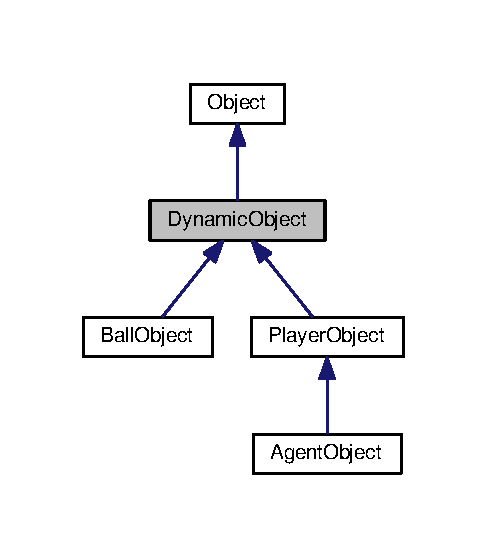
\includegraphics[width=234pt]{classDynamicObject__inherit__graph}
\end{center}
\end{figure}


Collaboration diagram for Dynamic\+Object\+:
\nopagebreak
\begin{figure}[H]
\begin{center}
\leavevmode
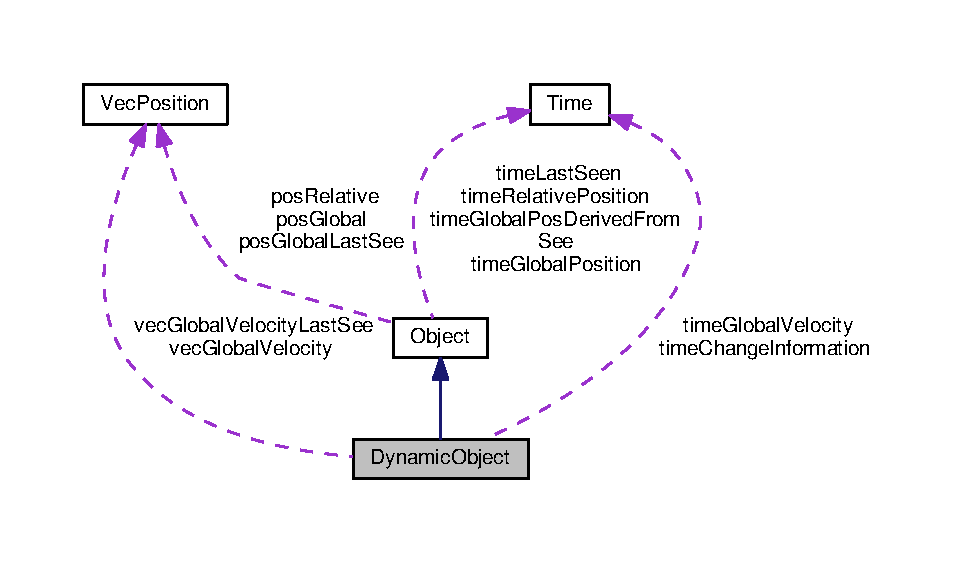
\includegraphics[width=350pt]{classDynamicObject__coll__graph}
\end{center}
\end{figure}
\subsection*{Public Member Functions}
\begin{DoxyCompactItemize}
\item 
\hyperlink{classDynamicObject_a50a7adf3d7d1f411ed2aa9a663bfe275}{Dynamic\+Object} ()
\item 
bool \hyperlink{classDynamicObject_ace3f0247ccbee18b060700e29cdaecfa}{set\+Relative\+Distance\+Change} (double d, \hyperlink{classTime}{Time} time)
\item 
double \hyperlink{classDynamicObject_a01e5c91446a97159dea6d7b55758ccf6}{get\+Relative\+Distance\+Change} () const 
\item 
bool \hyperlink{classDynamicObject_a8430113772bf1a1d53dd59d29217ed83}{set\+Relative\+Angle\+Change} (double d, \hyperlink{classTime}{Time} time)
\item 
double \hyperlink{classDynamicObject_a58c9e65e972c30b05a1e1196edadab00}{get\+Relative\+Angle\+Change} () const 
\item 
bool \hyperlink{classDynamicObject_ae1ddbb4b84bb8d7096541eef9f15c3cb}{set\+Time\+Change\+Information} (\hyperlink{classTime}{Time} time)
\item 
\hyperlink{classTime}{Time} \hyperlink{classDynamicObject_a0912aa0aec8a67175463576e9b15fc49}{get\+Time\+Change\+Information} () const 
\item 
bool \hyperlink{classDynamicObject_aca8b9324090abaee722a3366781b3876}{set\+Global\+Velocity} (\hyperlink{classVecPosition}{Vec\+Position} v, \hyperlink{classTime}{Time} time)
\item 
\hyperlink{classVecPosition}{Vec\+Position} \hyperlink{classDynamicObject_a35d2822999116ed8c0187322083efa63}{get\+Global\+Velocity} () const 
\item 
double \hyperlink{classDynamicObject_a3bd37ea0678865322cf0891325edebe0}{get\+Speed} () const 
\item 
bool \hyperlink{classDynamicObject_a1793d8c9a716fbaa8629578bbd22955b}{set\+Time\+Global\+Velocity} (\hyperlink{classTime}{Time} time)
\item 
\hyperlink{classTime}{Time} \hyperlink{classDynamicObject_aad3d5947f0432aa45fffd80d0ca06bf4}{get\+Time\+Global\+Velocity} () const 
\item 
bool \hyperlink{classDynamicObject_adfd0fffaff1853186cc1d9d04a4530f0}{set\+Global\+Velocity\+Last\+See} (\hyperlink{classVecPosition}{Vec\+Position} vec)
\item 
\hyperlink{classVecPosition}{Vec\+Position} \hyperlink{classDynamicObject_a9e72fbe37e1908f862d84cfd7a6da434}{get\+Global\+Velocity\+Last\+See} () const 
\end{DoxyCompactItemize}
\subsection*{Protected Attributes}
\begin{DoxyCompactItemize}
\item 
\hyperlink{classVecPosition}{Vec\+Position} \hyperlink{classDynamicObject_a64067c37d37e3484fea758cf388586e2}{vec\+Global\+Velocity}
\item 
\hyperlink{classTime}{Time} \hyperlink{classDynamicObject_a145bad5d089c8bcb80fbc797efa32e41}{time\+Global\+Velocity}
\item 
double \hyperlink{classDynamicObject_a3997feabd9a1705e48e78e4ecf5c709d}{d\+Relative\+Distance\+Change}
\item 
double \hyperlink{classDynamicObject_ab99ba16d2c8526f809832f28aa0d0824}{d\+Relative\+Angle\+Change}
\item 
\hyperlink{classTime}{Time} \hyperlink{classDynamicObject_a865b3a9f9e6c65da265ae11c5e96b28e}{time\+Change\+Information}
\item 
\hyperlink{classVecPosition}{Vec\+Position} \hyperlink{classDynamicObject_a61dfb8e440f2f045dccfb1b8e3759bae}{vec\+Global\+Velocity\+Last\+See}
\end{DoxyCompactItemize}


\subsection{Detailed Description}
Class \hyperlink{classDynamicObject}{Dynamic\+Object} contains Robo\+Cup information that is available for objects that can move (players, ball). Different variables are added to the superclass \hyperlink{classObject}{Object} 

\subsection{Constructor \& Destructor Documentation}
\index{Dynamic\+Object@{Dynamic\+Object}!Dynamic\+Object@{Dynamic\+Object}}
\index{Dynamic\+Object@{Dynamic\+Object}!Dynamic\+Object@{Dynamic\+Object}}
\subsubsection[{\texorpdfstring{Dynamic\+Object()}{DynamicObject()}}]{\setlength{\rightskip}{0pt plus 5cm}Dynamic\+Object\+::\+Dynamic\+Object (
\begin{DoxyParamCaption}
{}
\end{DoxyParamCaption}
)}\hypertarget{classDynamicObject_a50a7adf3d7d1f411ed2aa9a663bfe275}{}\label{classDynamicObject_a50a7adf3d7d1f411ed2aa9a663bfe275}
This is the constructor for \hyperlink{classDynamicObject}{Dynamic\+Object}. A \hyperlink{classDynamicObject}{Dynamic\+Object} is created with all the variables initialized by (illegal) default values 

\subsection{Member Function Documentation}
\index{Dynamic\+Object@{Dynamic\+Object}!get\+Global\+Velocity@{get\+Global\+Velocity}}
\index{get\+Global\+Velocity@{get\+Global\+Velocity}!Dynamic\+Object@{Dynamic\+Object}}
\subsubsection[{\texorpdfstring{get\+Global\+Velocity() const }{getGlobalVelocity() const }}]{\setlength{\rightskip}{0pt plus 5cm}{\bf Vec\+Position} Dynamic\+Object\+::get\+Global\+Velocity (
\begin{DoxyParamCaption}
{}
\end{DoxyParamCaption}
) const}\hypertarget{classDynamicObject_a35d2822999116ed8c0187322083efa63}{}\label{classDynamicObject_a35d2822999116ed8c0187322083efa63}
This method returns the global velocity of this object. The time of this information is related to the time returned by \hyperlink{classDynamicObject_aad3d5947f0432aa45fffd80d0ca06bf4}{get\+Time\+Global\+Velocity()}. \begin{DoxyReturn}{Returns}
global position of this object 
\end{DoxyReturn}
\index{Dynamic\+Object@{Dynamic\+Object}!get\+Global\+Velocity\+Last\+See@{get\+Global\+Velocity\+Last\+See}}
\index{get\+Global\+Velocity\+Last\+See@{get\+Global\+Velocity\+Last\+See}!Dynamic\+Object@{Dynamic\+Object}}
\subsubsection[{\texorpdfstring{get\+Global\+Velocity\+Last\+See() const }{getGlobalVelocityLastSee() const }}]{\setlength{\rightskip}{0pt plus 5cm}{\bf Vec\+Position} Dynamic\+Object\+::get\+Global\+Velocity\+Last\+See (
\begin{DoxyParamCaption}
{}
\end{DoxyParamCaption}
) const}\hypertarget{classDynamicObject_a9e72fbe37e1908f862d84cfd7a6da434}{}\label{classDynamicObject_a9e72fbe37e1908f862d84cfd7a6da434}
This method returns the global velocity of the object calculated after the last see message. The time of this information corresponds to \textquotesingle{}get\+Time\+Change\+Information\textquotesingle{}. \begin{DoxyReturn}{Returns}
global body velocity derived from the last see message 
\end{DoxyReturn}
\index{Dynamic\+Object@{Dynamic\+Object}!get\+Relative\+Angle\+Change@{get\+Relative\+Angle\+Change}}
\index{get\+Relative\+Angle\+Change@{get\+Relative\+Angle\+Change}!Dynamic\+Object@{Dynamic\+Object}}
\subsubsection[{\texorpdfstring{get\+Relative\+Angle\+Change() const }{getRelativeAngleChange() const }}]{\setlength{\rightskip}{0pt plus 5cm}double Dynamic\+Object\+::get\+Relative\+Angle\+Change (
\begin{DoxyParamCaption}
{}
\end{DoxyParamCaption}
) const}\hypertarget{classDynamicObject_a58c9e65e972c30b05a1e1196edadab00}{}\label{classDynamicObject_a58c9e65e972c30b05a1e1196edadab00}
This method returns the relative angle change of this object. This information belongs to the server time that is returned by \hyperlink{classDynamicObject_a0912aa0aec8a67175463576e9b15fc49}{get\+Time\+Change\+Information()}. \begin{DoxyReturn}{Returns}
relative angle change of object in the last cycle 
\end{DoxyReturn}
\index{Dynamic\+Object@{Dynamic\+Object}!get\+Relative\+Distance\+Change@{get\+Relative\+Distance\+Change}}
\index{get\+Relative\+Distance\+Change@{get\+Relative\+Distance\+Change}!Dynamic\+Object@{Dynamic\+Object}}
\subsubsection[{\texorpdfstring{get\+Relative\+Distance\+Change() const }{getRelativeDistanceChange() const }}]{\setlength{\rightskip}{0pt plus 5cm}double Dynamic\+Object\+::get\+Relative\+Distance\+Change (
\begin{DoxyParamCaption}
{}
\end{DoxyParamCaption}
) const}\hypertarget{classDynamicObject_a01e5c91446a97159dea6d7b55758ccf6}{}\label{classDynamicObject_a01e5c91446a97159dea6d7b55758ccf6}
This method returns the relative distance change of this object. Note that this value is zero when object is at the same distance, but at a complete different angle. This occurs when an object has moved a lot in one cycle. This information belongs to the server time that is returned by \hyperlink{classDynamicObject_a0912aa0aec8a67175463576e9b15fc49}{get\+Time\+Change\+Information()}. \begin{DoxyReturn}{Returns}
relative distance change of object in the last cycle 
\end{DoxyReturn}
\index{Dynamic\+Object@{Dynamic\+Object}!get\+Speed@{get\+Speed}}
\index{get\+Speed@{get\+Speed}!Dynamic\+Object@{Dynamic\+Object}}
\subsubsection[{\texorpdfstring{get\+Speed() const }{getSpeed() const }}]{\setlength{\rightskip}{0pt plus 5cm}double Dynamic\+Object\+::get\+Speed (
\begin{DoxyParamCaption}
{}
\end{DoxyParamCaption}
) const}\hypertarget{classDynamicObject_a3bd37ea0678865322cf0891325edebe0}{}\label{classDynamicObject_a3bd37ea0678865322cf0891325edebe0}
This method returns the speed of this object. The speed is the magnitude of the global velocity of the object \begin{DoxyReturn}{Returns}
speed of this object (zero for non-\/moving objects) 
\end{DoxyReturn}
\index{Dynamic\+Object@{Dynamic\+Object}!get\+Time\+Change\+Information@{get\+Time\+Change\+Information}}
\index{get\+Time\+Change\+Information@{get\+Time\+Change\+Information}!Dynamic\+Object@{Dynamic\+Object}}
\subsubsection[{\texorpdfstring{get\+Time\+Change\+Information() const }{getTimeChangeInformation() const }}]{\setlength{\rightskip}{0pt plus 5cm}{\bf Time} Dynamic\+Object\+::get\+Time\+Change\+Information (
\begin{DoxyParamCaption}
{}
\end{DoxyParamCaption}
) const}\hypertarget{classDynamicObject_a0912aa0aec8a67175463576e9b15fc49}{}\label{classDynamicObject_a0912aa0aec8a67175463576e9b15fc49}
This method returns the server time that belongs to the relative distance and relative angle change of this object. \begin{DoxyReturn}{Returns}
time of the change information of this \hyperlink{classDynamicObject}{Dynamic\+Object} 
\end{DoxyReturn}
\index{Dynamic\+Object@{Dynamic\+Object}!get\+Time\+Global\+Velocity@{get\+Time\+Global\+Velocity}}
\index{get\+Time\+Global\+Velocity@{get\+Time\+Global\+Velocity}!Dynamic\+Object@{Dynamic\+Object}}
\subsubsection[{\texorpdfstring{get\+Time\+Global\+Velocity() const }{getTimeGlobalVelocity() const }}]{\setlength{\rightskip}{0pt plus 5cm}{\bf Time} Dynamic\+Object\+::get\+Time\+Global\+Velocity (
\begin{DoxyParamCaption}
{}
\end{DoxyParamCaption}
) const}\hypertarget{classDynamicObject_aad3d5947f0432aa45fffd80d0ca06bf4}{}\label{classDynamicObject_aad3d5947f0432aa45fffd80d0ca06bf4}
This method returns the time that belongs to the global velocity of this object. \begin{DoxyReturn}{Returns}
time of the global velocity of this object 
\end{DoxyReturn}
\index{Dynamic\+Object@{Dynamic\+Object}!set\+Global\+Velocity@{set\+Global\+Velocity}}
\index{set\+Global\+Velocity@{set\+Global\+Velocity}!Dynamic\+Object@{Dynamic\+Object}}
\subsubsection[{\texorpdfstring{set\+Global\+Velocity(\+Vec\+Position v, Time time)}{setGlobalVelocity(VecPosition v, Time time)}}]{\setlength{\rightskip}{0pt plus 5cm}bool Dynamic\+Object\+::set\+Global\+Velocity (
\begin{DoxyParamCaption}
\item[{{\bf Vec\+Position}}]{v, }
\item[{{\bf Time}}]{time}
\end{DoxyParamCaption}
)}\hypertarget{classDynamicObject_aca8b9324090abaee722a3366781b3876}{}\label{classDynamicObject_aca8b9324090abaee722a3366781b3876}
This method sets the global velocity of this object and the time of this information 
\begin{DoxyParams}{Parameters}
{\em v} & new global velocity \\
\hline
{\em time} & time global velocity was received \\
\hline
\end{DoxyParams}
\begin{DoxyReturn}{Returns}
bool indicating whether the values were set 
\end{DoxyReturn}
\index{Dynamic\+Object@{Dynamic\+Object}!set\+Global\+Velocity\+Last\+See@{set\+Global\+Velocity\+Last\+See}}
\index{set\+Global\+Velocity\+Last\+See@{set\+Global\+Velocity\+Last\+See}!Dynamic\+Object@{Dynamic\+Object}}
\subsubsection[{\texorpdfstring{set\+Global\+Velocity\+Last\+See(\+Vec\+Position vec)}{setGlobalVelocityLastSee(VecPosition vec)}}]{\setlength{\rightskip}{0pt plus 5cm}bool Dynamic\+Object\+::set\+Global\+Velocity\+Last\+See (
\begin{DoxyParamCaption}
\item[{{\bf Vec\+Position}}]{vec}
\end{DoxyParamCaption}
)}\hypertarget{classDynamicObject_adfd0fffaff1853186cc1d9d04a4530f0}{}\label{classDynamicObject_adfd0fffaff1853186cc1d9d04a4530f0}
This method sets the global velocity of the object calculated after the last see message. The time of this information corresponds to \textquotesingle{}get\+Time\+Change\+Information\textquotesingle{}. \begin{DoxyReturn}{Returns}
global body velocity derived from the last see message 
\end{DoxyReturn}
\index{Dynamic\+Object@{Dynamic\+Object}!set\+Relative\+Angle\+Change@{set\+Relative\+Angle\+Change}}
\index{set\+Relative\+Angle\+Change@{set\+Relative\+Angle\+Change}!Dynamic\+Object@{Dynamic\+Object}}
\subsubsection[{\texorpdfstring{set\+Relative\+Angle\+Change(double d, Time time)}{setRelativeAngleChange(double d, Time time)}}]{\setlength{\rightskip}{0pt plus 5cm}bool Dynamic\+Object\+::set\+Relative\+Angle\+Change (
\begin{DoxyParamCaption}
\item[{double}]{d, }
\item[{{\bf Time}}]{time}
\end{DoxyParamCaption}
)}\hypertarget{classDynamicObject_a8430113772bf1a1d53dd59d29217ed83}{}\label{classDynamicObject_a8430113772bf1a1d53dd59d29217ed83}
This method sets the relative angle change and the server time this information belongs to. 
\begin{DoxyParams}{Parameters}
{\em d} & new relative angle change \\
\hline
{\em time} & time relative angle change was received \\
\hline
\end{DoxyParams}
\begin{DoxyReturn}{Returns}
bool indicating whether the values were set 
\end{DoxyReturn}
\index{Dynamic\+Object@{Dynamic\+Object}!set\+Relative\+Distance\+Change@{set\+Relative\+Distance\+Change}}
\index{set\+Relative\+Distance\+Change@{set\+Relative\+Distance\+Change}!Dynamic\+Object@{Dynamic\+Object}}
\subsubsection[{\texorpdfstring{set\+Relative\+Distance\+Change(double d, Time time)}{setRelativeDistanceChange(double d, Time time)}}]{\setlength{\rightskip}{0pt plus 5cm}bool Dynamic\+Object\+::set\+Relative\+Distance\+Change (
\begin{DoxyParamCaption}
\item[{double}]{d, }
\item[{{\bf Time}}]{time}
\end{DoxyParamCaption}
)}\hypertarget{classDynamicObject_ace3f0247ccbee18b060700e29cdaecfa}{}\label{classDynamicObject_ace3f0247ccbee18b060700e29cdaecfa}
This method sets the relative distance change and the time this information was calculated. 
\begin{DoxyParams}{Parameters}
{\em d} & new relative distance change \\
\hline
{\em time} & time relative distance change was calculated \\
\hline
\end{DoxyParams}
\begin{DoxyReturn}{Returns}
bool indicating whether the values were set 
\end{DoxyReturn}
\index{Dynamic\+Object@{Dynamic\+Object}!set\+Time\+Change\+Information@{set\+Time\+Change\+Information}}
\index{set\+Time\+Change\+Information@{set\+Time\+Change\+Information}!Dynamic\+Object@{Dynamic\+Object}}
\subsubsection[{\texorpdfstring{set\+Time\+Change\+Information(\+Time time)}{setTimeChangeInformation(Time time)}}]{\setlength{\rightskip}{0pt plus 5cm}bool Dynamic\+Object\+::set\+Time\+Change\+Information (
\begin{DoxyParamCaption}
\item[{{\bf Time}}]{time}
\end{DoxyParamCaption}
)}\hypertarget{classDynamicObject_ae1ddbb4b84bb8d7096541eef9f15c3cb}{}\label{classDynamicObject_ae1ddbb4b84bb8d7096541eef9f15c3cb}
This method sets the time the change information was calculated. 
\begin{DoxyParams}{Parameters}
{\em time} & time information for change was calculated \\
\hline
\end{DoxyParams}
\begin{DoxyReturn}{Returns}
bool indicating whether the values was set 
\end{DoxyReturn}
\index{Dynamic\+Object@{Dynamic\+Object}!set\+Time\+Global\+Velocity@{set\+Time\+Global\+Velocity}}
\index{set\+Time\+Global\+Velocity@{set\+Time\+Global\+Velocity}!Dynamic\+Object@{Dynamic\+Object}}
\subsubsection[{\texorpdfstring{set\+Time\+Global\+Velocity(\+Time time)}{setTimeGlobalVelocity(Time time)}}]{\setlength{\rightskip}{0pt plus 5cm}bool Dynamic\+Object\+::set\+Time\+Global\+Velocity (
\begin{DoxyParamCaption}
\item[{{\bf Time}}]{time}
\end{DoxyParamCaption}
)}\hypertarget{classDynamicObject_a1793d8c9a716fbaa8629578bbd22955b}{}\label{classDynamicObject_a1793d8c9a716fbaa8629578bbd22955b}
This method sets the time that corresponds to the last update of the global velocity of this object. 
\begin{DoxyParams}{Parameters}
{\em time} & time corresponding to current value of global velocity \\
\hline
\end{DoxyParams}
\begin{DoxyReturn}{Returns}
bool indicating whether the value was set 
\end{DoxyReturn}


\subsection{Member Data Documentation}
\index{Dynamic\+Object@{Dynamic\+Object}!d\+Relative\+Angle\+Change@{d\+Relative\+Angle\+Change}}
\index{d\+Relative\+Angle\+Change@{d\+Relative\+Angle\+Change}!Dynamic\+Object@{Dynamic\+Object}}
\subsubsection[{\texorpdfstring{d\+Relative\+Angle\+Change}{dRelativeAngleChange}}]{\setlength{\rightskip}{0pt plus 5cm}double Dynamic\+Object\+::d\+Relative\+Angle\+Change\hspace{0.3cm}{\ttfamily [protected]}}\hypertarget{classDynamicObject_ab99ba16d2c8526f809832f28aa0d0824}{}\label{classDynamicObject_ab99ba16d2c8526f809832f28aa0d0824}
Relative angle change \index{Dynamic\+Object@{Dynamic\+Object}!d\+Relative\+Distance\+Change@{d\+Relative\+Distance\+Change}}
\index{d\+Relative\+Distance\+Change@{d\+Relative\+Distance\+Change}!Dynamic\+Object@{Dynamic\+Object}}
\subsubsection[{\texorpdfstring{d\+Relative\+Distance\+Change}{dRelativeDistanceChange}}]{\setlength{\rightskip}{0pt plus 5cm}double Dynamic\+Object\+::d\+Relative\+Distance\+Change\hspace{0.3cm}{\ttfamily [protected]}}\hypertarget{classDynamicObject_a3997feabd9a1705e48e78e4ecf5c709d}{}\label{classDynamicObject_a3997feabd9a1705e48e78e4ecf5c709d}
Relative distance change \index{Dynamic\+Object@{Dynamic\+Object}!time\+Change\+Information@{time\+Change\+Information}}
\index{time\+Change\+Information@{time\+Change\+Information}!Dynamic\+Object@{Dynamic\+Object}}
\subsubsection[{\texorpdfstring{time\+Change\+Information}{timeChangeInformation}}]{\setlength{\rightskip}{0pt plus 5cm}{\bf Time} Dynamic\+Object\+::time\+Change\+Information\hspace{0.3cm}{\ttfamily [protected]}}\hypertarget{classDynamicObject_a865b3a9f9e6c65da265ae11c5e96b28e}{}\label{classDynamicObject_a865b3a9f9e6c65da265ae11c5e96b28e}
\hyperlink{classTime}{Time} of change information \index{Dynamic\+Object@{Dynamic\+Object}!time\+Global\+Velocity@{time\+Global\+Velocity}}
\index{time\+Global\+Velocity@{time\+Global\+Velocity}!Dynamic\+Object@{Dynamic\+Object}}
\subsubsection[{\texorpdfstring{time\+Global\+Velocity}{timeGlobalVelocity}}]{\setlength{\rightskip}{0pt plus 5cm}{\bf Time} Dynamic\+Object\+::time\+Global\+Velocity\hspace{0.3cm}{\ttfamily [protected]}}\hypertarget{classDynamicObject_a145bad5d089c8bcb80fbc797efa32e41}{}\label{classDynamicObject_a145bad5d089c8bcb80fbc797efa32e41}
\hyperlink{classTime}{Time} of the corresponding velocity \index{Dynamic\+Object@{Dynamic\+Object}!vec\+Global\+Velocity@{vec\+Global\+Velocity}}
\index{vec\+Global\+Velocity@{vec\+Global\+Velocity}!Dynamic\+Object@{Dynamic\+Object}}
\subsubsection[{\texorpdfstring{vec\+Global\+Velocity}{vecGlobalVelocity}}]{\setlength{\rightskip}{0pt plus 5cm}{\bf Vec\+Position} Dynamic\+Object\+::vec\+Global\+Velocity\hspace{0.3cm}{\ttfamily [protected]}}\hypertarget{classDynamicObject_a64067c37d37e3484fea758cf388586e2}{}\label{classDynamicObject_a64067c37d37e3484fea758cf388586e2}
Global velocity of the player \index{Dynamic\+Object@{Dynamic\+Object}!vec\+Global\+Velocity\+Last\+See@{vec\+Global\+Velocity\+Last\+See}}
\index{vec\+Global\+Velocity\+Last\+See@{vec\+Global\+Velocity\+Last\+See}!Dynamic\+Object@{Dynamic\+Object}}
\subsubsection[{\texorpdfstring{vec\+Global\+Velocity\+Last\+See}{vecGlobalVelocityLastSee}}]{\setlength{\rightskip}{0pt plus 5cm}{\bf Vec\+Position} Dynamic\+Object\+::vec\+Global\+Velocity\+Last\+See\hspace{0.3cm}{\ttfamily [protected]}}\hypertarget{classDynamicObject_a61dfb8e440f2f045dccfb1b8e3759bae}{}\label{classDynamicObject_a61dfb8e440f2f045dccfb1b8e3759bae}
vel. derived from last see 

The documentation for this class was generated from the following files\+:\begin{DoxyCompactItemize}
\item 
src/\hyperlink{Objects_8h}{Objects.\+h}\item 
src/\hyperlink{Objects_8cpp}{Objects.\+cpp}\end{DoxyCompactItemize}

\hypertarget{classFeature}{}\section{Feature Class Reference}
\label{classFeature}\index{Feature@{Feature}}


{\ttfamily \#include $<$Soccer\+Types.\+h$>$}

\subsection*{Public Member Functions}
\begin{DoxyCompactItemize}
\item 
\hyperlink{classFeature_a06d191f6daea88e0029440a2137f2e07}{Feature} ()
\item 
\hyperlink{classFeature_a01cfe1198d0d9483f6d7196d8371c921}{Feature} (\hyperlink{classTime}{Time} time\+See, \hyperlink{classTime}{Time} time\+Sense, \hyperlink{classTime}{Time} time\+Hear, \hyperlink{SoccerTypes_8h_ad4b701fa66e7d26c054ed15b7820c77c}{ObjectT} object, double d\+Info=\hyperlink{SoccerTypes_8h_ab232b103c74e1770db1120be5bae9be5}{Unknown\+Double\+Value}, \hyperlink{classSoccerCommand}{Soccer\+Command} soc=\hyperlink{classSoccerCommand}{Soccer\+Command}(\hyperlink{SoccerTypes_8h_ac986daf8a835e88572b79bcb63f5bbd5a38bf205bc1abc83eb30942d4e6511783}{C\+M\+D\+\_\+\+I\+L\+L\+E\+G\+AL}), \hyperlink{classVecPosition}{Vec\+Position} pos=\hyperlink{classVecPosition}{Vec\+Position}(0, 0))
\item 
bool \hyperlink{classFeature_ac66b87f375acc915a31dd3eaa1ab6db9}{set\+Feature} (\hyperlink{classTime}{Time} time\+See, \hyperlink{classTime}{Time} time\+Sense, \hyperlink{classTime}{Time} time\+Hear, \hyperlink{SoccerTypes_8h_ad4b701fa66e7d26c054ed15b7820c77c}{ObjectT} object, double d\+Info=\hyperlink{SoccerTypes_8h_ab232b103c74e1770db1120be5bae9be5}{Unknown\+Double\+Value}, \hyperlink{classSoccerCommand}{Soccer\+Command} soc=\hyperlink{classSoccerCommand}{Soccer\+Command}(\hyperlink{SoccerTypes_8h_ac986daf8a835e88572b79bcb63f5bbd5a38bf205bc1abc83eb30942d4e6511783}{C\+M\+D\+\_\+\+I\+L\+L\+E\+G\+AL}), \hyperlink{classVecPosition}{Vec\+Position} pos=\hyperlink{classVecPosition}{Vec\+Position}(0, 0))
\item 
bool \hyperlink{classFeature_a24e0447de2e87c722b5bf5a900510c9a}{set\+Time\+See} (\hyperlink{classTime}{Time} time)
\item 
\hyperlink{classTime}{Time} \hyperlink{classFeature_a4a9c3a4e9a59bb8d16d4a393dfe95a09}{get\+Time\+See} ()
\item 
bool \hyperlink{classFeature_a1a6c52bd5ab1cc70ffe39a1c20a9a556}{set\+Time\+Sense} (\hyperlink{classTime}{Time} time)
\item 
\hyperlink{classTime}{Time} \hyperlink{classFeature_a9f68128c0ba804df00bc1d25da03c65b}{get\+Time\+Sense} ()
\item 
bool \hyperlink{classFeature_af282805fca320ed0e087dde342ee6e79}{set\+Time\+Hear} (\hyperlink{classTime}{Time} time)
\item 
\hyperlink{classTime}{Time} \hyperlink{classFeature_a2a4657d2b0acd10c5ab5c547dbfaa85f}{get\+Time\+Hear} ()
\item 
bool \hyperlink{classFeature_af710a974e8dcd80c439a7a6ad6c00bb4}{set\+Object} (\hyperlink{SoccerTypes_8h_ad4b701fa66e7d26c054ed15b7820c77c}{ObjectT} obj)
\item 
\hyperlink{SoccerTypes_8h_ad4b701fa66e7d26c054ed15b7820c77c}{ObjectT} \hyperlink{classFeature_acf5901a189ac10a41cb7a3e17fa053de}{get\+Object} ()
\item 
bool \hyperlink{classFeature_a7c2fee01599f7d0cfd4ece91ee8ea145}{set\+Info} (double d)
\item 
double \hyperlink{classFeature_a9c83fc848f317203cd1af047fa2e87b1}{get\+Info} ()
\item 
bool \hyperlink{classFeature_ab0f96ebb874191c1adba7cdf22cc2086}{set\+Vec} (\hyperlink{classVecPosition}{Vec\+Position} pos)
\item 
\hyperlink{classVecPosition}{Vec\+Position} \hyperlink{classFeature_a2e35795fe923586d5292b1bc782f834a}{get\+Vec} ()
\item 
bool \hyperlink{classFeature_a875f14699302699f2ca7cb0a9d311627}{set\+Command} (\hyperlink{classSoccerCommand}{Soccer\+Command} soc)
\item 
\hyperlink{classSoccerCommand}{Soccer\+Command} \hyperlink{classFeature_abfdd2bfd5de65dceee55c862356cfe8d}{get\+Command} ()
\end{DoxyCompactItemize}


\subsection{Detailed Description}
This class contains information for one specific feature (e.\+g., fastest teammate to the ball. A feature corresponds to a specific time and is often related to a specific object and a specific value. Therefore, these values are stored in this class. 

\subsection{Constructor \& Destructor Documentation}
\index{Feature@{Feature}!Feature@{Feature}}
\index{Feature@{Feature}!Feature@{Feature}}
\subsubsection[{\texorpdfstring{Feature()}{Feature()}}]{\setlength{\rightskip}{0pt plus 5cm}Feature\+::\+Feature (
\begin{DoxyParamCaption}
{}
\end{DoxyParamCaption}
)}\hypertarget{classFeature_a06d191f6daea88e0029440a2137f2e07}{}\label{classFeature_a06d191f6daea88e0029440a2137f2e07}
This is the constructor for the \hyperlink{classFeature}{Feature} class. A feature (specific information that applies to the current time can be stored here. \index{Feature@{Feature}!Feature@{Feature}}
\index{Feature@{Feature}!Feature@{Feature}}
\subsubsection[{\texorpdfstring{Feature(\+Time time\+See, Time time\+Sense, Time time\+Hear, Object\+T object, double d\+Info=\+Unknown\+Double\+Value, Soccer\+Command soc=\+Soccer\+Command(\+C\+M\+D\+\_\+\+I\+L\+L\+E\+G\+A\+L), Vec\+Position pos=\+Vec\+Position(0, 0))}{Feature(Time timeSee, Time timeSense, Time timeHear, ObjectT object, double dInfo=UnknownDoubleValue, SoccerCommand soc=SoccerCommand(CMD_ILLEGAL), VecPosition pos=VecPosition(0, 0))}}]{\setlength{\rightskip}{0pt plus 5cm}Feature\+::\+Feature (
\begin{DoxyParamCaption}
\item[{{\bf Time}}]{time\+See, }
\item[{{\bf Time}}]{time\+Sense, }
\item[{{\bf Time}}]{time\+Hear, }
\item[{{\bf ObjectT}}]{object, }
\item[{double}]{d\+Info = {\ttfamily {\bf Unknown\+Double\+Value}}, }
\item[{{\bf Soccer\+Command}}]{soc = {\ttfamily {\bf Soccer\+Command}({\bf C\+M\+D\+\_\+\+I\+L\+L\+E\+G\+AL})}, }
\item[{{\bf Vec\+Position}}]{pos = {\ttfamily {\bf Vec\+Position}(0,0)}}
\end{DoxyParamCaption}
)}\hypertarget{classFeature_a01cfe1198d0d9483f6d7196d8371c921}{}\label{classFeature_a01cfe1198d0d9483f6d7196d8371c921}
This is the constructor for the \hyperlink{classFeature}{Feature} class. A feature (specific information that applies to the current time can be stored here. For example, when the information about the fastest player to the ball is calculated, this can be stored in a feauture. This information can then be used for another calculation in the same cycle. 
\begin{DoxyParams}{Parameters}
{\em time\+See} & time of see message to which this feature applies. \\
\hline
{\em time\+Sense} & time of sense message to which this feature applies. \\
\hline
{\em object} & object to which this feature applies \\
\hline
{\em d\+Info} & specific information that can be stored about this feature. \\
\hline
{\em soc} & soccercommand stored with this feature \\
\hline
{\em pos} & position information stored with this feature \\
\hline
\end{DoxyParams}


\subsection{Member Function Documentation}
\index{Feature@{Feature}!get\+Command@{get\+Command}}
\index{get\+Command@{get\+Command}!Feature@{Feature}}
\subsubsection[{\texorpdfstring{get\+Command()}{getCommand()}}]{\setlength{\rightskip}{0pt plus 5cm}{\bf Soccer\+Command} Feature\+::get\+Command (
\begin{DoxyParamCaption}
{}
\end{DoxyParamCaption}
)}\hypertarget{classFeature_abfdd2bfd5de65dceee55c862356cfe8d}{}\label{classFeature_abfdd2bfd5de65dceee55c862356cfe8d}
This method returns the command corresponding to this feature. \begin{DoxyReturn}{Returns}
command stored with this feature. 
\end{DoxyReturn}
\index{Feature@{Feature}!get\+Info@{get\+Info}}
\index{get\+Info@{get\+Info}!Feature@{Feature}}
\subsubsection[{\texorpdfstring{get\+Info()}{getInfo()}}]{\setlength{\rightskip}{0pt plus 5cm}double Feature\+::get\+Info (
\begin{DoxyParamCaption}
{}
\end{DoxyParamCaption}
)}\hypertarget{classFeature_a9c83fc848f317203cd1af047fa2e87b1}{}\label{classFeature_a9c83fc848f317203cd1af047fa2e87b1}
This method returns the information for a feature. \begin{DoxyReturn}{Returns}
information stored with this feature. 
\end{DoxyReturn}
\index{Feature@{Feature}!get\+Object@{get\+Object}}
\index{get\+Object@{get\+Object}!Feature@{Feature}}
\subsubsection[{\texorpdfstring{get\+Object()}{getObject()}}]{\setlength{\rightskip}{0pt plus 5cm}{\bf ObjectT} Feature\+::get\+Object (
\begin{DoxyParamCaption}
{}
\end{DoxyParamCaption}
)}\hypertarget{classFeature_acf5901a189ac10a41cb7a3e17fa053de}{}\label{classFeature_acf5901a189ac10a41cb7a3e17fa053de}
This method returns the object related to this feature. \begin{DoxyReturn}{Returns}
object stored with this feature. 
\end{DoxyReturn}
\index{Feature@{Feature}!get\+Time\+Hear@{get\+Time\+Hear}}
\index{get\+Time\+Hear@{get\+Time\+Hear}!Feature@{Feature}}
\subsubsection[{\texorpdfstring{get\+Time\+Hear()}{getTimeHear()}}]{\setlength{\rightskip}{0pt plus 5cm}{\bf Time} Feature\+::get\+Time\+Hear (
\begin{DoxyParamCaption}
{}
\end{DoxyParamCaption}
)}\hypertarget{classFeature_a2a4657d2b0acd10c5ab5c547dbfaa85f}{}\label{classFeature_a2a4657d2b0acd10c5ab5c547dbfaa85f}
This method returns the hear time for a feature. \begin{DoxyReturn}{Returns}
time that is related to this feature. 
\end{DoxyReturn}
\index{Feature@{Feature}!get\+Time\+See@{get\+Time\+See}}
\index{get\+Time\+See@{get\+Time\+See}!Feature@{Feature}}
\subsubsection[{\texorpdfstring{get\+Time\+See()}{getTimeSee()}}]{\setlength{\rightskip}{0pt plus 5cm}{\bf Time} Feature\+::get\+Time\+See (
\begin{DoxyParamCaption}
{}
\end{DoxyParamCaption}
)}\hypertarget{classFeature_a4a9c3a4e9a59bb8d16d4a393dfe95a09}{}\label{classFeature_a4a9c3a4e9a59bb8d16d4a393dfe95a09}
This method returns the see time for a feature. \begin{DoxyReturn}{Returns}
time that is related to this feature. 
\end{DoxyReturn}
\index{Feature@{Feature}!get\+Time\+Sense@{get\+Time\+Sense}}
\index{get\+Time\+Sense@{get\+Time\+Sense}!Feature@{Feature}}
\subsubsection[{\texorpdfstring{get\+Time\+Sense()}{getTimeSense()}}]{\setlength{\rightskip}{0pt plus 5cm}{\bf Time} Feature\+::get\+Time\+Sense (
\begin{DoxyParamCaption}
{}
\end{DoxyParamCaption}
)}\hypertarget{classFeature_a9f68128c0ba804df00bc1d25da03c65b}{}\label{classFeature_a9f68128c0ba804df00bc1d25da03c65b}
This method returns the sense time for a feature. \begin{DoxyReturn}{Returns}
time that is related to this feature. 
\end{DoxyReturn}
\index{Feature@{Feature}!get\+Vec@{get\+Vec}}
\index{get\+Vec@{get\+Vec}!Feature@{Feature}}
\subsubsection[{\texorpdfstring{get\+Vec()}{getVec()}}]{\setlength{\rightskip}{0pt plus 5cm}{\bf Vec\+Position} Feature\+::get\+Vec (
\begin{DoxyParamCaption}
{}
\end{DoxyParamCaption}
)}\hypertarget{classFeature_a2e35795fe923586d5292b1bc782f834a}{}\label{classFeature_a2e35795fe923586d5292b1bc782f834a}
This method returns the position information for a feature. \begin{DoxyReturn}{Returns}
position information stored with this feature. 
\end{DoxyReturn}
\index{Feature@{Feature}!set\+Command@{set\+Command}}
\index{set\+Command@{set\+Command}!Feature@{Feature}}
\subsubsection[{\texorpdfstring{set\+Command(\+Soccer\+Command soc)}{setCommand(SoccerCommand soc)}}]{\setlength{\rightskip}{0pt plus 5cm}bool Feature\+::set\+Command (
\begin{DoxyParamCaption}
\item[{{\bf Soccer\+Command}}]{soc}
\end{DoxyParamCaption}
)}\hypertarget{classFeature_a875f14699302699f2ca7cb0a9d311627}{}\label{classFeature_a875f14699302699f2ca7cb0a9d311627}
This method sets the command corresponding to this feature. \begin{DoxyReturn}{Returns}
boolean indicating whether update was succesfull. 
\end{DoxyReturn}
\index{Feature@{Feature}!set\+Feature@{set\+Feature}}
\index{set\+Feature@{set\+Feature}!Feature@{Feature}}
\subsubsection[{\texorpdfstring{set\+Feature(\+Time time\+See, Time time\+Sense, Time time\+Hear, Object\+T object, double d\+Info=\+Unknown\+Double\+Value, Soccer\+Command soc=\+Soccer\+Command(\+C\+M\+D\+\_\+\+I\+L\+L\+E\+G\+A\+L), Vec\+Position pos=\+Vec\+Position(0, 0))}{setFeature(Time timeSee, Time timeSense, Time timeHear, ObjectT object, double dInfo=UnknownDoubleValue, SoccerCommand soc=SoccerCommand(CMD_ILLEGAL), VecPosition pos=VecPosition(0, 0))}}]{\setlength{\rightskip}{0pt plus 5cm}bool Feature\+::set\+Feature (
\begin{DoxyParamCaption}
\item[{{\bf Time}}]{time\+See, }
\item[{{\bf Time}}]{time\+Sense, }
\item[{{\bf Time}}]{time\+Hear, }
\item[{{\bf ObjectT}}]{object, }
\item[{double}]{d\+Info = {\ttfamily {\bf Unknown\+Double\+Value}}, }
\item[{{\bf Soccer\+Command}}]{soc = {\ttfamily {\bf Soccer\+Command}({\bf C\+M\+D\+\_\+\+I\+L\+L\+E\+G\+AL})}, }
\item[{{\bf Vec\+Position}}]{pos = {\ttfamily {\bf Vec\+Position}(0,0)}}
\end{DoxyParamCaption}
)}\hypertarget{classFeature_ac66b87f375acc915a31dd3eaa1ab6db9}{}\label{classFeature_ac66b87f375acc915a31dd3eaa1ab6db9}
This methods sets the values of the \hyperlink{classFeature}{Feature} class. A feature (specific information that applies to the current time can be stored here. For example, when the information about the fastest player to the ball is calculated, this can be stored in a feauture. This information can then be used for another calculation in the same cycle. 
\begin{DoxyParams}{Parameters}
{\em time\+See} & time of see message to which this feature applies. \\
\hline
{\em time\+Sense} & time of sense message to which this feature applies. \\
\hline
{\em time\+Sense} & time of hear message to which this feature applies. \\
\hline
{\em object} & object to which this feature applies \\
\hline
{\em d\+Info} & specific information that can be stored about this feature. \\
\hline
{\em soc} & command stored with this feature \\
\hline
{\em pos} & position information stored with this feature \\
\hline
\end{DoxyParams}
\begin{DoxyReturn}{Returns}
boolean indicating whether update was successful. 
\end{DoxyReturn}
\index{Feature@{Feature}!set\+Info@{set\+Info}}
\index{set\+Info@{set\+Info}!Feature@{Feature}}
\subsubsection[{\texorpdfstring{set\+Info(double d)}{setInfo(double d)}}]{\setlength{\rightskip}{0pt plus 5cm}bool Feature\+::set\+Info (
\begin{DoxyParamCaption}
\item[{double}]{d}
\end{DoxyParamCaption}
)}\hypertarget{classFeature_a7c2fee01599f7d0cfd4ece91ee8ea145}{}\label{classFeature_a7c2fee01599f7d0cfd4ece91ee8ea145}
This method sets the information for a feature. 
\begin{DoxyParams}{Parameters}
{\em d} & double information that applies to this feature. \\
\hline
\end{DoxyParams}
\index{Feature@{Feature}!set\+Object@{set\+Object}}
\index{set\+Object@{set\+Object}!Feature@{Feature}}
\subsubsection[{\texorpdfstring{set\+Object(\+Object\+T obj)}{setObject(ObjectT obj)}}]{\setlength{\rightskip}{0pt plus 5cm}bool Feature\+::set\+Object (
\begin{DoxyParamCaption}
\item[{{\bf ObjectT}}]{object}
\end{DoxyParamCaption}
)}\hypertarget{classFeature_af710a974e8dcd80c439a7a6ad6c00bb4}{}\label{classFeature_af710a974e8dcd80c439a7a6ad6c00bb4}
This method sets the object for a feature. 
\begin{DoxyParams}{Parameters}
{\em object} & object type that applies to this feature. \\
\hline
\end{DoxyParams}
\index{Feature@{Feature}!set\+Time\+Hear@{set\+Time\+Hear}}
\index{set\+Time\+Hear@{set\+Time\+Hear}!Feature@{Feature}}
\subsubsection[{\texorpdfstring{set\+Time\+Hear(\+Time time)}{setTimeHear(Time time)}}]{\setlength{\rightskip}{0pt plus 5cm}bool Feature\+::set\+Time\+Hear (
\begin{DoxyParamCaption}
\item[{{\bf Time}}]{time}
\end{DoxyParamCaption}
)}\hypertarget{classFeature_af282805fca320ed0e087dde342ee6e79}{}\label{classFeature_af282805fca320ed0e087dde342ee6e79}
This method sets the hear time for a feature. 
\begin{DoxyParams}{Parameters}
{\em time} & hear time that applies to this feature. \\
\hline
\end{DoxyParams}
\index{Feature@{Feature}!set\+Time\+See@{set\+Time\+See}}
\index{set\+Time\+See@{set\+Time\+See}!Feature@{Feature}}
\subsubsection[{\texorpdfstring{set\+Time\+See(\+Time time)}{setTimeSee(Time time)}}]{\setlength{\rightskip}{0pt plus 5cm}bool Feature\+::set\+Time\+See (
\begin{DoxyParamCaption}
\item[{{\bf Time}}]{time}
\end{DoxyParamCaption}
)}\hypertarget{classFeature_a24e0447de2e87c722b5bf5a900510c9a}{}\label{classFeature_a24e0447de2e87c722b5bf5a900510c9a}
This method sets the see time for a feature. 
\begin{DoxyParams}{Parameters}
{\em time} & see time that applies to this feature. \\
\hline
\end{DoxyParams}
\index{Feature@{Feature}!set\+Time\+Sense@{set\+Time\+Sense}}
\index{set\+Time\+Sense@{set\+Time\+Sense}!Feature@{Feature}}
\subsubsection[{\texorpdfstring{set\+Time\+Sense(\+Time time)}{setTimeSense(Time time)}}]{\setlength{\rightskip}{0pt plus 5cm}bool Feature\+::set\+Time\+Sense (
\begin{DoxyParamCaption}
\item[{{\bf Time}}]{time}
\end{DoxyParamCaption}
)}\hypertarget{classFeature_a1a6c52bd5ab1cc70ffe39a1c20a9a556}{}\label{classFeature_a1a6c52bd5ab1cc70ffe39a1c20a9a556}
This method sets the sense time for a feature. 
\begin{DoxyParams}{Parameters}
{\em time} & sense time that applies to this feature. \\
\hline
\end{DoxyParams}
\index{Feature@{Feature}!set\+Vec@{set\+Vec}}
\index{set\+Vec@{set\+Vec}!Feature@{Feature}}
\subsubsection[{\texorpdfstring{set\+Vec(\+Vec\+Position pos)}{setVec(VecPosition pos)}}]{\setlength{\rightskip}{0pt plus 5cm}bool Feature\+::set\+Vec (
\begin{DoxyParamCaption}
\item[{{\bf Vec\+Position}}]{pos}
\end{DoxyParamCaption}
)}\hypertarget{classFeature_ab0f96ebb874191c1adba7cdf22cc2086}{}\label{classFeature_ab0f96ebb874191c1adba7cdf22cc2086}
This method sets the posiiton corresponding to this feature. \begin{DoxyReturn}{Returns}
boolean indicating whether update was succesfull. 
\end{DoxyReturn}


The documentation for this class was generated from the following files\+:\begin{DoxyCompactItemize}
\item 
src/\hyperlink{SoccerTypes_8h}{Soccer\+Types.\+h}\item 
src/\hyperlink{SoccerTypes_8cpp}{Soccer\+Types.\+cpp}\end{DoxyCompactItemize}

\hypertarget{classFixedObject}{}\section{Fixed\+Object Class Reference}
\label{classFixedObject}\index{Fixed\+Object@{Fixed\+Object}}


{\ttfamily \#include $<$Objects.\+h$>$}



Inheritance diagram for Fixed\+Object\+:
\nopagebreak
\begin{figure}[H]
\begin{center}
\leavevmode
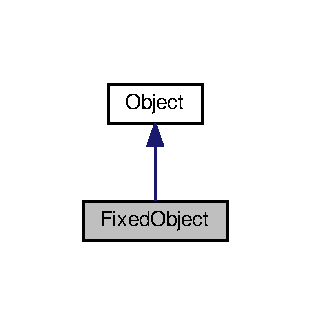
\includegraphics[width=149pt]{classFixedObject__inherit__graph}
\end{center}
\end{figure}


Collaboration diagram for Fixed\+Object\+:
\nopagebreak
\begin{figure}[H]
\begin{center}
\leavevmode
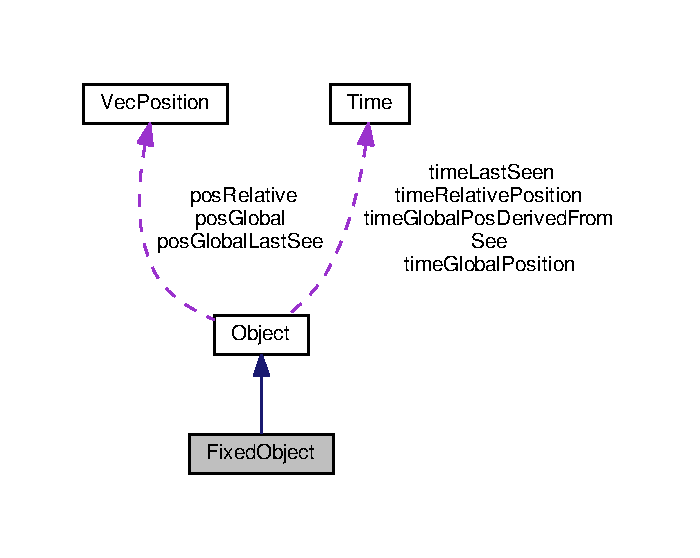
\includegraphics[width=336pt]{classFixedObject__coll__graph}
\end{center}
\end{figure}
\subsection*{Public Member Functions}
\begin{DoxyCompactItemize}
\item 
\hyperlink{classVecPosition}{Vec\+Position} \hyperlink{classFixedObject_a7a50b54f0ca18257ab3d45afb3fd816c}{get\+Global\+Position} (\hyperlink{SoccerTypes_8h_a8e9b8119c00121a197203aca01d5b090}{SideT} s, double d\+Goal\+Width=14.\+02) const 
\item 
\hyperlink{Geometry_8h_a6bfe02ae9bb185092902092561ab2865}{Ang\+Deg} \hyperlink{classFixedObject_abcbfb2537519c3328a896b3b44070ea6}{get\+Global\+Angle} (\hyperlink{SoccerTypes_8h_a8e9b8119c00121a197203aca01d5b090}{SideT} s)
\item 
void \hyperlink{classFixedObject_ad8771b36cc2073d4a9fe1879b2f91d06}{show} (ostream \&os=cout)
\end{DoxyCompactItemize}
\subsection*{Additional Inherited Members}


\subsection{Detailed Description}
Class \hyperlink{classFixedObject}{Fixed\+Object} contains Robo\+Cup information that is available for objects that cannot move (flags, goals, lines). No additional information is added to the superclass \hyperlink{classObject}{Object}. 

\subsection{Member Function Documentation}
\index{Fixed\+Object@{Fixed\+Object}!get\+Global\+Angle@{get\+Global\+Angle}}
\index{get\+Global\+Angle@{get\+Global\+Angle}!Fixed\+Object@{Fixed\+Object}}
\subsubsection[{\texorpdfstring{get\+Global\+Angle(\+Side\+T s)}{getGlobalAngle(SideT s)}}]{\setlength{\rightskip}{0pt plus 5cm}{\bf Ang\+Deg} Fixed\+Object\+::get\+Global\+Angle (
\begin{DoxyParamCaption}
\item[{{\bf SideT}}]{s}
\end{DoxyParamCaption}
)}\hypertarget{classFixedObject_abcbfb2537519c3328a896b3b44070ea6}{}\label{classFixedObject_abcbfb2537519c3328a896b3b44070ea6}
This methods returns the global angle of this fixed object in the world. Only works when the fixed object is a line. The angle for the left team rises clockwise, i.\+e. left=0, bottom=90, etc. For the right team this is counterclockwise\+: right=0, top=90, etc) 
\begin{DoxyParams}{Parameters}
{\em s} & side of agent (angles differ for left and right side) \\
\hline
\end{DoxyParams}
\begin{DoxyReturn}{Returns}
global angle of this line in the world. 
\end{DoxyReturn}
\index{Fixed\+Object@{Fixed\+Object}!get\+Global\+Position@{get\+Global\+Position}}
\index{get\+Global\+Position@{get\+Global\+Position}!Fixed\+Object@{Fixed\+Object}}
\subsubsection[{\texorpdfstring{get\+Global\+Position(\+Side\+T s, double d\+Goal\+Width=14.\+02) const }{getGlobalPosition(SideT s, double dGoalWidth=14.02) const }}]{\setlength{\rightskip}{0pt plus 5cm}{\bf Vec\+Position} Fixed\+Object\+::get\+Global\+Position (
\begin{DoxyParamCaption}
\item[{{\bf SideT}}]{s, }
\item[{double}]{d\+Goal\+Width = {\ttfamily 14.02}}
\end{DoxyParamCaption}
) const}\hypertarget{classFixedObject_a7a50b54f0ca18257ab3d45afb3fd816c}{}\label{classFixedObject_a7a50b54f0ca18257ab3d45afb3fd816c}
This method returns the global position of this fixed object. Only works when the object type equals a flag or a goal. Furthermore the side of the agent has to be passed since the global positions differ for the left and the right side. For some flags the size of the goal is important. So this value can be passed also. Otherwise the default value is 14.\+02. 
\begin{DoxyParams}{Parameters}
{\em s} & side of agent (global position differs for left and right side) \\
\hline
{\em d\+Goal\+Width} & width of a goal, needed for pole objects next to goal \\
\hline
\end{DoxyParams}
\begin{DoxyReturn}{Returns}
global position of this fixed object. 
\end{DoxyReturn}
\index{Fixed\+Object@{Fixed\+Object}!show@{show}}
\index{show@{show}!Fixed\+Object@{Fixed\+Object}}
\subsubsection[{\texorpdfstring{show(ostream \&os=cout)}{show(ostream &os=cout)}}]{\setlength{\rightskip}{0pt plus 5cm}void Fixed\+Object\+::show (
\begin{DoxyParamCaption}
\item[{ostream \&}]{os = {\ttfamily cout}}
\end{DoxyParamCaption}
)\hspace{0.3cm}{\ttfamily [virtual]}}\hypertarget{classFixedObject_ad8771b36cc2073d4a9fe1879b2f91d06}{}\label{classFixedObject_ad8771b36cc2073d4a9fe1879b2f91d06}
This method prints all the information about this \hyperlink{classFixedObject}{Fixed\+Object} to the specified output stream 
\begin{DoxyParams}{Parameters}
{\em os} & output stream to print all relevant information to. \\
\hline
\end{DoxyParams}


Implements \hyperlink{classObject_abdfad2372e7ec5f9aa271a1677653778}{Object}.



The documentation for this class was generated from the following files\+:\begin{DoxyCompactItemize}
\item 
src/\hyperlink{Objects_8h}{Objects.\+h}\item 
src/\hyperlink{Objects_8cpp}{Objects.\+cpp}\end{DoxyCompactItemize}

\hypertarget{classFormations}{}\section{Formations Class Reference}
\label{classFormations}\index{Formations@{Formations}}


{\ttfamily \#include $<$Formations.\+h$>$}

\subsection*{Public Member Functions}
\begin{DoxyCompactItemize}
\item 
\hyperlink{classFormations_a264876ee1cc41fa6e1fd7af65f56301e}{Formations} (const char $\ast$str\+File=N\+U\+LL, \hyperlink{SoccerTypes_8h_ac803bd9e3400705765031836994a385d}{FormationT} ft=\hyperlink{SoccerTypes_8h_ac803bd9e3400705765031836994a385dadf3294904b0ea24dce056d2b043429cb}{F\+T\+\_\+\+I\+L\+L\+E\+G\+AL}, int i\+Nr=1)
\item 
void \hyperlink{classFormations_a120210db61d594900bdcf06b3d33f778}{show} (ostream \&os=cout)
\item 
\hyperlink{classVecPosition}{Vec\+Position} \hyperlink{classFormations_aa22f05f42980c91bf785d781cdc550e4}{get\+Strategic\+Position} (int i\+Player, \hyperlink{classVecPosition}{Vec\+Position} pos\+Ball, double d\+Max\+X\+In\+Play\+Mode, bool b\+In\+Ball\+Possession=false, double d\+Max\+Y\+Percentage=0.\+75, \hyperlink{SoccerTypes_8h_ac803bd9e3400705765031836994a385d}{FormationT} ft=\hyperlink{SoccerTypes_8h_ac803bd9e3400705765031836994a385dadf3294904b0ea24dce056d2b043429cb}{F\+T\+\_\+\+I\+L\+L\+E\+G\+AL})
\item 
bool \hyperlink{classFormations_ac5c2bad0ac7fba6c9174b56fd13bfca7}{read\+Formations} (const char $\ast$str\+File)
\item 
bool \hyperlink{classFormations_a3cf04d1c4b05f8875c34f8e01eda5ca5}{set\+Formation} (\hyperlink{SoccerTypes_8h_ac803bd9e3400705765031836994a385d}{FormationT} formation)
\item 
\hyperlink{SoccerTypes_8h_ac803bd9e3400705765031836994a385d}{FormationT} \hyperlink{classFormations_a42e9372f624ce25d39426671a48c027c}{get\+Formation} () const 
\item 
bool \hyperlink{classFormations_a6940f63f7337071facfdb8ebc84a9eb7}{set\+Player\+In\+Formation} (int number)
\item 
int \hyperlink{classFormations_ab6f6349508af032911ec00c038246d98}{get\+Player\+In\+Formation} (\hyperlink{SoccerTypes_8h_ad4b701fa66e7d26c054ed15b7820c77c}{ObjectT} obj=\hyperlink{SoccerTypes_8h_ad4b701fa66e7d26c054ed15b7820c77cae887ec2051f19c0708a9a34df06e87a9}{O\+B\+J\+E\+C\+T\+\_\+\+I\+L\+L\+E\+G\+AL}) const 
\item 
\hyperlink{SoccerTypes_8h_a88daf580b042467ccd4098107cffc718}{PlayerT} \hyperlink{classFormations_aeb476d961e67951300683265e66ff022}{get\+Player\+Type} (\hyperlink{SoccerTypes_8h_ad4b701fa66e7d26c054ed15b7820c77c}{ObjectT} obj, \hyperlink{SoccerTypes_8h_ac803bd9e3400705765031836994a385d}{FormationT} ft=\hyperlink{SoccerTypes_8h_ac803bd9e3400705765031836994a385dadf3294904b0ea24dce056d2b043429cb}{F\+T\+\_\+\+I\+L\+L\+E\+G\+AL}) const 
\item 
\hyperlink{SoccerTypes_8h_a88daf580b042467ccd4098107cffc718}{PlayerT} \hyperlink{classFormations_ae5167443b6f3d0c26f08de7e53d20f48}{get\+Player\+Type} (int i\+Index=-\/1, \hyperlink{SoccerTypes_8h_ac803bd9e3400705765031836994a385d}{FormationT} ft=\hyperlink{SoccerTypes_8h_ac803bd9e3400705765031836994a385dadf3294904b0ea24dce056d2b043429cb}{F\+T\+\_\+\+I\+L\+L\+E\+G\+AL}) const 
\end{DoxyCompactItemize}


\subsection{Detailed Description}
This class is a container for all different Formation Types\+: it contains the information of all the formation types. Furthermore it contains two other values\+: the current formation type that is used by the agent and the role of the agent in the current formation. These two values fully specify the position of this player in the formation. 

\subsection{Constructor \& Destructor Documentation}
\index{Formations@{Formations}!Formations@{Formations}}
\index{Formations@{Formations}!Formations@{Formations}}
\subsubsection[{\texorpdfstring{Formations(const char $\ast$str\+File=\+N\+U\+L\+L, Formation\+T ft=\+F\+T\+\_\+\+I\+L\+L\+E\+G\+A\+L, int i\+Nr=1)}{Formations(const char *strFile=NULL, FormationT ft=FT_ILLEGAL, int iNr=1)}}]{\setlength{\rightskip}{0pt plus 5cm}Formations\+::\+Formations (
\begin{DoxyParamCaption}
\item[{const char $\ast$}]{str\+File = {\ttfamily NULL}, }
\item[{{\bf FormationT}}]{cur\+Ft = {\ttfamily {\bf F\+T\+\_\+\+I\+L\+L\+E\+G\+AL}}, }
\item[{int}]{i\+Nr = {\ttfamily 1}}
\end{DoxyParamCaption}
)}\hypertarget{classFormations_a264876ee1cc41fa6e1fd7af65f56301e}{}\label{classFormations_a264876ee1cc41fa6e1fd7af65f56301e}
This is the constructor for the \hyperlink{classFormations}{Formations} class and needs as arguments a formation configuration file, the current formation and the number of the agent in this formation (normally at start-\/up this equals the player number). 
\begin{DoxyParams}{Parameters}
{\em str\+File} & string representation of the formation configuration file \\
\hline
{\em cur\+Ft} & current formation type (default F\+T\+\_\+\+I\+L\+L\+E\+G\+AL) \\
\hline
{\em i\+Nr} & number of the agent in this formation (default 1) \\
\hline
\end{DoxyParams}


\subsection{Member Function Documentation}
\index{Formations@{Formations}!get\+Formation@{get\+Formation}}
\index{get\+Formation@{get\+Formation}!Formations@{Formations}}
\subsubsection[{\texorpdfstring{get\+Formation() const }{getFormation() const }}]{\setlength{\rightskip}{0pt plus 5cm}{\bf FormationT} Formations\+::get\+Formation (
\begin{DoxyParamCaption}
{}
\end{DoxyParamCaption}
) const}\hypertarget{classFormations_a42e9372f624ce25d39426671a48c027c}{}\label{classFormations_a42e9372f624ce25d39426671a48c027c}
This method returns the current formation. \begin{DoxyReturn}{Returns}
current formation 
\end{DoxyReturn}
\index{Formations@{Formations}!get\+Player\+In\+Formation@{get\+Player\+In\+Formation}}
\index{get\+Player\+In\+Formation@{get\+Player\+In\+Formation}!Formations@{Formations}}
\subsubsection[{\texorpdfstring{get\+Player\+In\+Formation(\+Object\+T obj=\+O\+B\+J\+E\+C\+T\+\_\+\+I\+L\+L\+E\+G\+A\+L) const }{getPlayerInFormation(ObjectT obj=OBJECT_ILLEGAL) const }}]{\setlength{\rightskip}{0pt plus 5cm}int Formations\+::get\+Player\+In\+Formation (
\begin{DoxyParamCaption}
\item[{{\bf ObjectT}}]{obj = {\ttfamily {\bf O\+B\+J\+E\+C\+T\+\_\+\+I\+L\+L\+E\+G\+AL}}}
\end{DoxyParamCaption}
) const}\hypertarget{classFormations_ab6f6349508af032911ec00c038246d98}{}\label{classFormations_ab6f6349508af032911ec00c038246d98}
This method returns the role number of the agent in the current formation \begin{DoxyReturn}{Returns}
player number for this agent in the current formation 
\end{DoxyReturn}
\index{Formations@{Formations}!get\+Player\+Type@{get\+Player\+Type}}
\index{get\+Player\+Type@{get\+Player\+Type}!Formations@{Formations}}
\subsubsection[{\texorpdfstring{get\+Player\+Type(\+Object\+T obj, Formation\+T ft=\+F\+T\+\_\+\+I\+L\+L\+E\+G\+A\+L) const }{getPlayerType(ObjectT obj, FormationT ft=FT_ILLEGAL) const }}]{\setlength{\rightskip}{0pt plus 5cm}{\bf PlayerT} Formations\+::get\+Player\+Type (
\begin{DoxyParamCaption}
\item[{{\bf ObjectT}}]{obj, }
\item[{{\bf FormationT}}]{ft = {\ttfamily {\bf F\+T\+\_\+\+I\+L\+L\+E\+G\+AL}}}
\end{DoxyParamCaption}
) const}\hypertarget{classFormations_aeb476d961e67951300683265e66ff022}{}\label{classFormations_aeb476d961e67951300683265e66ff022}
This method returns the player type for the specified object \begin{DoxyReturn}{Returns}
player type for the agent in the current formation 
\end{DoxyReturn}
\index{Formations@{Formations}!get\+Player\+Type@{get\+Player\+Type}}
\index{get\+Player\+Type@{get\+Player\+Type}!Formations@{Formations}}
\subsubsection[{\texorpdfstring{get\+Player\+Type(int i\+Index=-\/1, Formation\+T ft=\+F\+T\+\_\+\+I\+L\+L\+E\+G\+A\+L) const }{getPlayerType(int iIndex=-1, FormationT ft=FT_ILLEGAL) const }}]{\setlength{\rightskip}{0pt plus 5cm}{\bf PlayerT} Formations\+::get\+Player\+Type (
\begin{DoxyParamCaption}
\item[{int}]{i\+Index = {\ttfamily -\/1}, }
\item[{{\bf FormationT}}]{ft = {\ttfamily {\bf F\+T\+\_\+\+I\+L\+L\+E\+G\+AL}}}
\end{DoxyParamCaption}
) const}\hypertarget{classFormations_ae5167443b6f3d0c26f08de7e53d20f48}{}\label{classFormations_ae5167443b6f3d0c26f08de7e53d20f48}
This method returns the player type for the agent in the current formation \begin{DoxyReturn}{Returns}
player type for the agent in the current formation 
\end{DoxyReturn}
\index{Formations@{Formations}!get\+Strategic\+Position@{get\+Strategic\+Position}}
\index{get\+Strategic\+Position@{get\+Strategic\+Position}!Formations@{Formations}}
\subsubsection[{\texorpdfstring{get\+Strategic\+Position(int i\+Player, Vec\+Position pos\+Ball, double d\+Max\+X\+In\+Play\+Mode, bool b\+In\+Ball\+Possession=false, double d\+Max\+Y\+Percentage=0.\+75, Formation\+T ft=\+F\+T\+\_\+\+I\+L\+L\+E\+G\+A\+L)}{getStrategicPosition(int iPlayer, VecPosition posBall, double dMaxXInPlayMode, bool bInBallPossession=false, double dMaxYPercentage=0.75, FormationT ft=FT_ILLEGAL)}}]{\setlength{\rightskip}{0pt plus 5cm}{\bf Vec\+Position} Formations\+::get\+Strategic\+Position (
\begin{DoxyParamCaption}
\item[{int}]{i\+Player, }
\item[{{\bf Vec\+Position}}]{pos\+Ball, }
\item[{double}]{d\+Max\+X\+In\+Play\+Mode, }
\item[{bool}]{b\+In\+Ball\+Possession = {\ttfamily false}, }
\item[{double}]{d\+Max\+Y\+Percentage = {\ttfamily 0.75}, }
\item[{{\bf FormationT}}]{ft = {\ttfamily {\bf F\+T\+\_\+\+I\+L\+L\+E\+G\+AL}}}
\end{DoxyParamCaption}
)}\hypertarget{classFormations_aa22f05f42980c91bf785d781cdc550e4}{}\label{classFormations_aa22f05f42980c91bf785d781cdc550e4}
This method returns the strategic position for a player. It calculates this information by taking the home position of the current role in the current formation and combines this with the position of the ball using the attraction values for the current player type. The attraction values defines the percentage of the ball coordinate that is added to the home position of the current player type. So when the x coordindate of the home position is 10.\+0, x coordinate ball is 20.\+0 and x attraction is 0.\+25. The x coordinate of the strategic position will become 10.\+0 + 0.\+25$\ast$20.0 = 15.\+0. When this value is smaller than the minimal x coordinate or larger than the maximal x coordinate, the coordinate is changed to this minimal or maximal coordinate respectively. Also when the behind ball value is set, the x coordinate of the strategic position is set to this ball coordinate. Furthermore when the strategic position is in front of the supplied argument d\+Max\+X\+In\+Play\+Mode, the x coordinate is adjusted to this value. During normal play mode the supplied value is often the offside line. 
\begin{DoxyParams}{Parameters}
{\em i\+Player} & player number in formation of which strategic position should be determined. \\
\hline
{\em pos\+Ball} & position of the ball \\
\hline
{\em d\+Max\+X\+In\+Play\+Mode,max} & x coordinate allowed in current play mode. \\
\hline
\end{DoxyParams}
\index{Formations@{Formations}!read\+Formations@{read\+Formations}}
\index{read\+Formations@{read\+Formations}!Formations@{Formations}}
\subsubsection[{\texorpdfstring{read\+Formations(const char $\ast$str\+File)}{readFormations(const char *strFile)}}]{\setlength{\rightskip}{0pt plus 5cm}bool Formations\+::read\+Formations (
\begin{DoxyParamCaption}
\item[{const char $\ast$}]{str\+File}
\end{DoxyParamCaption}
)}\hypertarget{classFormations_ac5c2bad0ac7fba6c9174b56fd13bfca7}{}\label{classFormations_ac5c2bad0ac7fba6c9174b56fd13bfca7}
This method reads the formations from the file \textquotesingle{}str\+File\textquotesingle{} and has the following format\+:
\begin{DoxyItemize}
\item x coordinate of the home position for all the roles
\item y coordinate of the home position for all the roles
\item the player types for all the roles
\item the x attraction for all the player types
\item the y attraction for all the player types
\item indication whether to stay behind the ball for all the player types
\item minimal x coordinate for all the player types
\item maximal x coordinate for all the player types
\item extra y distance added to strat. pos. when in ball possession 
\begin{DoxyParams}{Parameters}
{\em str\+File} & string representation of the file. \\
\hline
\end{DoxyParams}
\begin{DoxyReturn}{Returns}
bool when file was read in succesfully. 
\end{DoxyReturn}

\end{DoxyItemize}\index{Formations@{Formations}!set\+Formation@{set\+Formation}}
\index{set\+Formation@{set\+Formation}!Formations@{Formations}}
\subsubsection[{\texorpdfstring{set\+Formation(\+Formation\+T formation)}{setFormation(FormationT formation)}}]{\setlength{\rightskip}{0pt plus 5cm}bool Formations\+::set\+Formation (
\begin{DoxyParamCaption}
\item[{{\bf FormationT}}]{formation}
\end{DoxyParamCaption}
)}\hypertarget{classFormations_a3cf04d1c4b05f8875c34f8e01eda5ca5}{}\label{classFormations_a3cf04d1c4b05f8875c34f8e01eda5ca5}
This method sets the current formation. 
\begin{DoxyParams}{Parameters}
{\em formation} & new current formation \\
\hline
\end{DoxyParams}
\begin{DoxyReturn}{Returns}
bool indicating whether the update was successful 
\end{DoxyReturn}
\index{Formations@{Formations}!set\+Player\+In\+Formation@{set\+Player\+In\+Formation}}
\index{set\+Player\+In\+Formation@{set\+Player\+In\+Formation}!Formations@{Formations}}
\subsubsection[{\texorpdfstring{set\+Player\+In\+Formation(int number)}{setPlayerInFormation(int number)}}]{\setlength{\rightskip}{0pt plus 5cm}bool Formations\+::set\+Player\+In\+Formation (
\begin{DoxyParamCaption}
\item[{int}]{i\+Number}
\end{DoxyParamCaption}
)}\hypertarget{classFormations_a6940f63f7337071facfdb8ebc84a9eb7}{}\label{classFormations_a6940f63f7337071facfdb8ebc84a9eb7}
This method sets the player number of the agent in the current formation to \textquotesingle{}i\+Number\textquotesingle{}. 
\begin{DoxyParams}{Parameters}
{\em i\+Number} & new player number for this agent \\
\hline
\end{DoxyParams}
\begin{DoxyReturn}{Returns}
bool indicating whether the update was succesfull 
\end{DoxyReturn}
\index{Formations@{Formations}!show@{show}}
\index{show@{show}!Formations@{Formations}}
\subsubsection[{\texorpdfstring{show(ostream \&os=cout)}{show(ostream &os=cout)}}]{\setlength{\rightskip}{0pt plus 5cm}void Formations\+::show (
\begin{DoxyParamCaption}
\item[{ostream \&}]{os = {\ttfamily cout}}
\end{DoxyParamCaption}
)}\hypertarget{classFormations_a120210db61d594900bdcf06b3d33f778}{}\label{classFormations_a120210db61d594900bdcf06b3d33f778}
This methods prints all the information of the different formation types to the output stream os and furthermore prints the current formation and the role number of the agent in this formation. 
\begin{DoxyParams}{Parameters}
{\em os} & output stream to which output is written. \\
\hline
\end{DoxyParams}


The documentation for this class was generated from the following files\+:\begin{DoxyCompactItemize}
\item 
src/\hyperlink{Formations_8h}{Formations.\+h}\item 
src/\hyperlink{Formations_8cpp}{Formations.\+cpp}\end{DoxyCompactItemize}

\hypertarget{classFormationTypeInfo}{}\section{Formation\+Type\+Info Class Reference}
\label{classFormationTypeInfo}\index{Formation\+Type\+Info@{Formation\+Type\+Info}}


{\ttfamily \#include $<$Formations.\+h$>$}

\subsection*{Public Member Functions}
\begin{DoxyCompactItemize}
\item 
\hyperlink{classFormationTypeInfo_a6cc97e2eefc63bfa2fed24d22845e5b1}{Formation\+Type\+Info} ()
\item 
void \hyperlink{classFormationTypeInfo_a073e49de1ee750c4b84b50c2d80bf2fa}{show} (ostream \&os=cout)
\item 
bool \hyperlink{classFormationTypeInfo_a0fcee6c47ac6aa4757b93d0fd3db9523}{set\+Formation\+Type} (\hyperlink{SoccerTypes_8h_ac803bd9e3400705765031836994a385d}{FormationT} type)
\item 
\hyperlink{SoccerTypes_8h_ac803bd9e3400705765031836994a385d}{FormationT} \hyperlink{classFormationTypeInfo_ace4194c4963192814d8cb51dbca77a1f}{get\+Formation\+Type} () const 
\item 
bool \hyperlink{classFormationTypeInfo_a457b72b71aee22843f7a5ef95a015e8c}{set\+Pos\+Home} (\hyperlink{classVecPosition}{Vec\+Position} pos, int at\+Index)
\item 
bool \hyperlink{classFormationTypeInfo_a3be9863c90a991d7525d911c43c7bb5a}{set\+X\+Pos\+Home} (double x, int at\+Index)
\item 
bool \hyperlink{classFormationTypeInfo_a76641da64e29137b142a9a5a4bb1657e}{set\+Y\+Pos\+Home} (double y, int at\+Index)
\item 
\hyperlink{classVecPosition}{Vec\+Position} \hyperlink{classFormationTypeInfo_a7df5f712623d4c33b3b21d591ed35404}{get\+Pos\+Home} (int at\+Index) const 
\item 
bool \hyperlink{classFormationTypeInfo_a5dc596bd06680f99becf797dae6bf558}{set\+Player\+Type} (\hyperlink{SoccerTypes_8h_a88daf580b042467ccd4098107cffc718}{PlayerT} type, int at\+Index)
\item 
\hyperlink{SoccerTypes_8h_a88daf580b042467ccd4098107cffc718}{PlayerT} \hyperlink{classFormationTypeInfo_a4e240cd93fd7cffd04aa6021ca9ffa57}{get\+Player\+Type} (int at\+Index) const 
\item 
bool \hyperlink{classFormationTypeInfo_ac16054807a993ca58956b0f36ec3c724}{set\+Player\+Type\+Info} (\hyperlink{classPlayerTypeInfo}{Player\+Type\+Info} info, int at\+Index)
\item 
\hyperlink{classPlayerTypeInfo}{Player\+Type\+Info} $\ast$ \hyperlink{classFormationTypeInfo_a9fcab63078eafecda0f85eeb4d5e3f4c}{get\+Player\+Type\+Info} (int at\+Index)
\item 
\hyperlink{classPlayerTypeInfo}{Player\+Type\+Info} $\ast$ \hyperlink{classFormationTypeInfo_a7e88263145ac65a029dd0bec6a543e76}{get\+Player\+Type\+Info\+Of\+Player} (int i\+Player\+In\+Formation)
\end{DoxyCompactItemize}


\subsection{Detailed Description}
This class contains information about one specific formation. It contains the formation type (defined in \hyperlink{SoccerTypes_8h}{Soccer\+Types.\+h}), the home position of all the roles (=specific player in a formation), the player types for all the roles and the information about the different player\+\_\+types. Furthermore it contains methods to retrieve this information for a specific role. 

\subsection{Constructor \& Destructor Documentation}
\index{Formation\+Type\+Info@{Formation\+Type\+Info}!Formation\+Type\+Info@{Formation\+Type\+Info}}
\index{Formation\+Type\+Info@{Formation\+Type\+Info}!Formation\+Type\+Info@{Formation\+Type\+Info}}
\subsubsection[{\texorpdfstring{Formation\+Type\+Info()}{FormationTypeInfo()}}]{\setlength{\rightskip}{0pt plus 5cm}Formation\+Type\+Info\+::\+Formation\+Type\+Info (
\begin{DoxyParamCaption}
{}
\end{DoxyParamCaption}
)}\hypertarget{classFormationTypeInfo_a6cc97e2eefc63bfa2fed24d22845e5b1}{}\label{classFormationTypeInfo_a6cc97e2eefc63bfa2fed24d22845e5b1}
This is the default constructor and does nothing. 

\subsection{Member Function Documentation}
\index{Formation\+Type\+Info@{Formation\+Type\+Info}!get\+Formation\+Type@{get\+Formation\+Type}}
\index{get\+Formation\+Type@{get\+Formation\+Type}!Formation\+Type\+Info@{Formation\+Type\+Info}}
\subsubsection[{\texorpdfstring{get\+Formation\+Type() const }{getFormationType() const }}]{\setlength{\rightskip}{0pt plus 5cm}{\bf FormationT} Formation\+Type\+Info\+::get\+Formation\+Type (
\begin{DoxyParamCaption}
{}
\end{DoxyParamCaption}
) const}\hypertarget{classFormationTypeInfo_ace4194c4963192814d8cb51dbca77a1f}{}\label{classFormationTypeInfo_ace4194c4963192814d8cb51dbca77a1f}
This method return the current formation type for this class. \begin{DoxyReturn}{Returns}
formation type for this class. 
\end{DoxyReturn}
\index{Formation\+Type\+Info@{Formation\+Type\+Info}!get\+Player\+Type@{get\+Player\+Type}}
\index{get\+Player\+Type@{get\+Player\+Type}!Formation\+Type\+Info@{Formation\+Type\+Info}}
\subsubsection[{\texorpdfstring{get\+Player\+Type(int at\+Index) const }{getPlayerType(int atIndex) const }}]{\setlength{\rightskip}{0pt plus 5cm}{\bf PlayerT} Formation\+Type\+Info\+::get\+Player\+Type (
\begin{DoxyParamCaption}
\item[{int}]{at\+Index}
\end{DoxyParamCaption}
) const}\hypertarget{classFormationTypeInfo_a4e240cd93fd7cffd04aa6021ca9ffa57}{}\label{classFormationTypeInfo_a4e240cd93fd7cffd04aa6021ca9ffa57}
This method returns the player type for the player with role number \textquotesingle{}at\+Index\textquotesingle{} in this formation. \begin{DoxyReturn}{Returns}
player type for player with role number \textquotesingle{}at\+Index\textquotesingle{} 
\end{DoxyReturn}
\index{Formation\+Type\+Info@{Formation\+Type\+Info}!get\+Player\+Type\+Info@{get\+Player\+Type\+Info}}
\index{get\+Player\+Type\+Info@{get\+Player\+Type\+Info}!Formation\+Type\+Info@{Formation\+Type\+Info}}
\subsubsection[{\texorpdfstring{get\+Player\+Type\+Info(int at\+Index)}{getPlayerTypeInfo(int atIndex)}}]{\setlength{\rightskip}{0pt plus 5cm}{\bf Player\+Type\+Info} $\ast$ Formation\+Type\+Info\+::get\+Player\+Type\+Info (
\begin{DoxyParamCaption}
\item[{int}]{at\+Index}
\end{DoxyParamCaption}
)}\hypertarget{classFormationTypeInfo_a9fcab63078eafecda0f85eeb4d5e3f4c}{}\label{classFormationTypeInfo_a9fcab63078eafecda0f85eeb4d5e3f4c}
This method returns (a pointer to) the player type information for the player type at position \textquotesingle{}at\+Index\textquotesingle{} 
\begin{DoxyParams}{Parameters}
{\em at\+Index} & index of which player type information should be returned \\
\hline
\end{DoxyParams}
\begin{DoxyReturn}{Returns}
pointer to player type information located at index \textquotesingle{}at\+Index\textquotesingle{} 
\end{DoxyReturn}
\index{Formation\+Type\+Info@{Formation\+Type\+Info}!get\+Player\+Type\+Info\+Of\+Player@{get\+Player\+Type\+Info\+Of\+Player}}
\index{get\+Player\+Type\+Info\+Of\+Player@{get\+Player\+Type\+Info\+Of\+Player}!Formation\+Type\+Info@{Formation\+Type\+Info}}
\subsubsection[{\texorpdfstring{get\+Player\+Type\+Info\+Of\+Player(int i\+Player\+In\+Formation)}{getPlayerTypeInfoOfPlayer(int iPlayerInFormation)}}]{\setlength{\rightskip}{0pt plus 5cm}{\bf Player\+Type\+Info} $\ast$ Formation\+Type\+Info\+::get\+Player\+Type\+Info\+Of\+Player (
\begin{DoxyParamCaption}
\item[{int}]{i\+Player\+In\+Formation}
\end{DoxyParamCaption}
)}\hypertarget{classFormationTypeInfo_a7e88263145ac65a029dd0bec6a543e76}{}\label{classFormationTypeInfo_a7e88263145ac65a029dd0bec6a543e76}
This method returns (a pointer to) the player type information for the player with role number \textquotesingle{}i\+Player\+In\+Formation\textquotesingle{}. 
\begin{DoxyParams}{Parameters}
{\em i\+Player\+In\+Formation} & role number for which info should be returned \\
\hline
\end{DoxyParams}
\begin{DoxyReturn}{Returns}
pointer to information for role \textquotesingle{}i\+Player\+In\+Formation\textquotesingle{} 
\end{DoxyReturn}
\index{Formation\+Type\+Info@{Formation\+Type\+Info}!get\+Pos\+Home@{get\+Pos\+Home}}
\index{get\+Pos\+Home@{get\+Pos\+Home}!Formation\+Type\+Info@{Formation\+Type\+Info}}
\subsubsection[{\texorpdfstring{get\+Pos\+Home(int at\+Index) const }{getPosHome(int atIndex) const }}]{\setlength{\rightskip}{0pt plus 5cm}{\bf Vec\+Position} Formation\+Type\+Info\+::get\+Pos\+Home (
\begin{DoxyParamCaption}
\item[{int}]{at\+Index}
\end{DoxyParamCaption}
) const}\hypertarget{classFormationTypeInfo_a7df5f712623d4c33b3b21d591ed35404}{}\label{classFormationTypeInfo_a7df5f712623d4c33b3b21d591ed35404}
This method returns the home position for the player with role number at\+Index in this formation. The home position is the position from which the strategic position is calculated and could be interpreted as the position a player is located when the ball is at the position (0,0). \begin{DoxyReturn}{Returns}
home position for player number at index \textquotesingle{}at\+Index\textquotesingle{} 
\end{DoxyReturn}
\index{Formation\+Type\+Info@{Formation\+Type\+Info}!set\+Formation\+Type@{set\+Formation\+Type}}
\index{set\+Formation\+Type@{set\+Formation\+Type}!Formation\+Type\+Info@{Formation\+Type\+Info}}
\subsubsection[{\texorpdfstring{set\+Formation\+Type(\+Formation\+T type)}{setFormationType(FormationT type)}}]{\setlength{\rightskip}{0pt plus 5cm}bool Formation\+Type\+Info\+::set\+Formation\+Type (
\begin{DoxyParamCaption}
\item[{{\bf FormationT}}]{type}
\end{DoxyParamCaption}
)}\hypertarget{classFormationTypeInfo_a0fcee6c47ac6aa4757b93d0fd3db9523}{}\label{classFormationTypeInfo_a0fcee6c47ac6aa4757b93d0fd3db9523}
This method sets the current formation type for this class. 
\begin{DoxyParams}{Parameters}
{\em type} & new formation type for this class. \\
\hline
\end{DoxyParams}
\begin{DoxyReturn}{Returns}
bool indicating whether update was successful. 
\end{DoxyReturn}
\index{Formation\+Type\+Info@{Formation\+Type\+Info}!set\+Player\+Type@{set\+Player\+Type}}
\index{set\+Player\+Type@{set\+Player\+Type}!Formation\+Type\+Info@{Formation\+Type\+Info}}
\subsubsection[{\texorpdfstring{set\+Player\+Type(\+Player\+T type, int at\+Index)}{setPlayerType(PlayerT type, int atIndex)}}]{\setlength{\rightskip}{0pt plus 5cm}bool Formation\+Type\+Info\+::set\+Player\+Type (
\begin{DoxyParamCaption}
\item[{{\bf PlayerT}}]{type, }
\item[{int}]{at\+Index}
\end{DoxyParamCaption}
)}\hypertarget{classFormationTypeInfo_a5dc596bd06680f99becf797dae6bf558}{}\label{classFormationTypeInfo_a5dc596bd06680f99becf797dae6bf558}
This method sets the player type for the player with role number \textquotesingle{}at\+Index\textquotesingle{} in this formation. 
\begin{DoxyParams}{Parameters}
{\em type} & new player type for role at position \textquotesingle{}at\+Index\textquotesingle{} \\
\hline
{\em at\+Index} & role number for which player type should be set. \\
\hline
\end{DoxyParams}
\begin{DoxyReturn}{Returns}
bool indicating whether update was succesfull. 
\end{DoxyReturn}
\index{Formation\+Type\+Info@{Formation\+Type\+Info}!set\+Player\+Type\+Info@{set\+Player\+Type\+Info}}
\index{set\+Player\+Type\+Info@{set\+Player\+Type\+Info}!Formation\+Type\+Info@{Formation\+Type\+Info}}
\subsubsection[{\texorpdfstring{set\+Player\+Type\+Info(\+Player\+Type\+Info info, int at\+Index)}{setPlayerTypeInfo(PlayerTypeInfo info, int atIndex)}}]{\setlength{\rightskip}{0pt plus 5cm}bool Formation\+Type\+Info\+::set\+Player\+Type\+Info (
\begin{DoxyParamCaption}
\item[{{\bf Player\+Type\+Info}}]{info, }
\item[{int}]{at\+Index}
\end{DoxyParamCaption}
)}\hypertarget{classFormationTypeInfo_ac16054807a993ca58956b0f36ec3c724}{}\label{classFormationTypeInfo_ac16054807a993ca58956b0f36ec3c724}
This method sets the information for a player type in this formation. Note that information is for a player T\+Y\+PE and not for a player R\+O\+LE. 
\begin{DoxyParams}{Parameters}
{\em info} & new player type information for the player type at \textquotesingle{}at\+Index\textquotesingle{}. \\
\hline
{\em at\+Index} & number of player type for which information should be set. \\
\hline
\end{DoxyParams}
\begin{DoxyReturn}{Returns}
bool indicating whether update was succesfull. 
\end{DoxyReturn}
\index{Formation\+Type\+Info@{Formation\+Type\+Info}!set\+Pos\+Home@{set\+Pos\+Home}}
\index{set\+Pos\+Home@{set\+Pos\+Home}!Formation\+Type\+Info@{Formation\+Type\+Info}}
\subsubsection[{\texorpdfstring{set\+Pos\+Home(\+Vec\+Position pos, int at\+Index)}{setPosHome(VecPosition pos, int atIndex)}}]{\setlength{\rightskip}{0pt plus 5cm}bool Formation\+Type\+Info\+::set\+Pos\+Home (
\begin{DoxyParamCaption}
\item[{{\bf Vec\+Position}}]{pos, }
\item[{int}]{at\+Index}
\end{DoxyParamCaption}
)}\hypertarget{classFormationTypeInfo_a457b72b71aee22843f7a5ef95a015e8c}{}\label{classFormationTypeInfo_a457b72b71aee22843f7a5ef95a015e8c}
This method sets the home position of the role indicated by the number \textquotesingle{}at\+Index\textquotesingle{} in this formation. The home position is the position from which the strategic position is calculated and could be interpreted as the position a player is located when the ball is at the position (0,0). 
\begin{DoxyParams}{Parameters}
{\em pos} & new home position for the player with role number \textquotesingle{}at\+Index\textquotesingle{} \\
\hline
{\em at\+Index} & index of the player with role for which the home position should be set. \\
\hline
\end{DoxyParams}
\begin{DoxyReturn}{Returns}
bool indicating whether update was succesfull. 
\end{DoxyReturn}
\index{Formation\+Type\+Info@{Formation\+Type\+Info}!set\+X\+Pos\+Home@{set\+X\+Pos\+Home}}
\index{set\+X\+Pos\+Home@{set\+X\+Pos\+Home}!Formation\+Type\+Info@{Formation\+Type\+Info}}
\subsubsection[{\texorpdfstring{set\+X\+Pos\+Home(double x, int at\+Index)}{setXPosHome(double x, int atIndex)}}]{\setlength{\rightskip}{0pt plus 5cm}bool Formation\+Type\+Info\+::set\+X\+Pos\+Home (
\begin{DoxyParamCaption}
\item[{double}]{x, }
\item[{int}]{at\+Index}
\end{DoxyParamCaption}
)}\hypertarget{classFormationTypeInfo_a3be9863c90a991d7525d911c43c7bb5a}{}\label{classFormationTypeInfo_a3be9863c90a991d7525d911c43c7bb5a}
This method sets the x coordinate of the home position for the player with role number \textquotesingle{}at\+Index\textquotesingle{}. 
\begin{DoxyParams}{Parameters}
{\em x} & x coordinate for the home position \\
\hline
{\em at\+Index} & role in formation for which x coordinate should be set. \\
\hline
\end{DoxyParams}
\begin{DoxyReturn}{Returns}
bool indicating whether update was succesfull. 
\end{DoxyReturn}
\index{Formation\+Type\+Info@{Formation\+Type\+Info}!set\+Y\+Pos\+Home@{set\+Y\+Pos\+Home}}
\index{set\+Y\+Pos\+Home@{set\+Y\+Pos\+Home}!Formation\+Type\+Info@{Formation\+Type\+Info}}
\subsubsection[{\texorpdfstring{set\+Y\+Pos\+Home(double y, int at\+Index)}{setYPosHome(double y, int atIndex)}}]{\setlength{\rightskip}{0pt plus 5cm}bool Formation\+Type\+Info\+::set\+Y\+Pos\+Home (
\begin{DoxyParamCaption}
\item[{double}]{y, }
\item[{int}]{at\+Index}
\end{DoxyParamCaption}
)}\hypertarget{classFormationTypeInfo_a76641da64e29137b142a9a5a4bb1657e}{}\label{classFormationTypeInfo_a76641da64e29137b142a9a5a4bb1657e}
This method sets the y coordinate of the home position for the player with role number \textquotesingle{}at\+Index\textquotesingle{}. 
\begin{DoxyParams}{Parameters}
{\em y} & y coordinate for the home position \\
\hline
{\em at\+Index} & role number for which y coordinate should be set. \\
\hline
\end{DoxyParams}
\begin{DoxyReturn}{Returns}
bool indicating whether update was succesfull. 
\end{DoxyReturn}
\index{Formation\+Type\+Info@{Formation\+Type\+Info}!show@{show}}
\index{show@{show}!Formation\+Type\+Info@{Formation\+Type\+Info}}
\subsubsection[{\texorpdfstring{show(ostream \&os=cout)}{show(ostream &os=cout)}}]{\setlength{\rightskip}{0pt plus 5cm}void Formation\+Type\+Info\+::show (
\begin{DoxyParamCaption}
\item[{ostream \&}]{os = {\ttfamily cout}}
\end{DoxyParamCaption}
)}\hypertarget{classFormationTypeInfo_a073e49de1ee750c4b84b50c2d80bf2fa}{}\label{classFormationTypeInfo_a073e49de1ee750c4b84b50c2d80bf2fa}
This method prints all the information about this formation to the specified output stream. The format is the following\+:
\begin{DoxyItemize}
\item x coordinate of the home position for all the roles
\item y coordinate of the home position for all the roles
\item the player types for all the roles
\item the x attraction for all the player types
\item the y attraction for all the player types
\item indication whether to stay behind the ball for all the player types
\item minimal x coordinate for all the player types
\item maximal x coordinate for all the player types 
\begin{DoxyParams}{Parameters}
{\em os} & output stream for output. \\
\hline
\end{DoxyParams}

\end{DoxyItemize}

The documentation for this class was generated from the following files\+:\begin{DoxyCompactItemize}
\item 
src/\hyperlink{Formations_8h}{Formations.\+h}\item 
src/\hyperlink{Formations_8cpp}{Formations.\+cpp}\end{DoxyCompactItemize}

\hypertarget{classGenericValues}{}\section{Generic\+Values Class Reference}
\label{classGenericValues}\index{Generic\+Values@{Generic\+Values}}


{\ttfamily \#include $<$Generic\+Values.\+h$>$}



Inheritance diagram for Generic\+Values\+:
\nopagebreak
\begin{figure}[H]
\begin{center}
\leavevmode
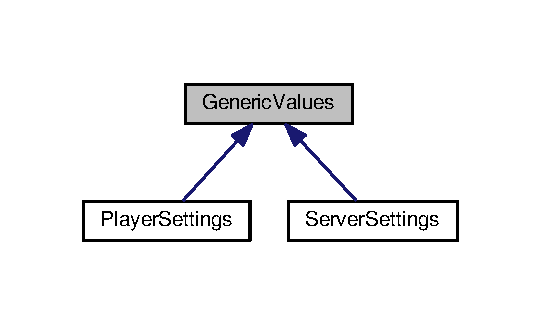
\includegraphics[width=260pt]{classGenericValues__inherit__graph}
\end{center}
\end{figure}
\subsection*{Public Member Functions}
\begin{DoxyCompactItemize}
\item 
\hyperlink{classGenericValues_a292b8984daf043d89e6101ffe2a91d39}{Generic\+Values} (const char $\ast$str\+Name, int i\+Max\+Values)
\item 
virtual \hyperlink{classGenericValues_a6e44fb16050936c76930294bf33d1897}{$\sim$\+Generic\+Values} ()
\item 
char $\ast$ \hyperlink{classGenericValues_a5f1cde2b4413db0e19d1d1f2f97fc7bb}{get\+Class\+Name} ()
\item 
int \hyperlink{classGenericValues_a2dabc28295d3c2d2173ff83953731988}{get\+Values\+Total} ()
\item 
bool \hyperlink{classGenericValues_af733534c2df3eadf5d113193bf1cd569}{add\+Setting} (const char $\ast$str\+Name, void $\ast$v\+Address, \hyperlink{GenericValues_8h_aaecaa3e46488aab71938a199e362d0c6}{Generic\+Value\+Kind} t)
\item 
virtual char $\ast$ \hyperlink{classGenericValues_a9c1f39be5e66e2137378eee180f57aff}{get\+Value} (const char $\ast$str\+Name, char $\ast$str\+Value)
\item 
virtual bool \hyperlink{classGenericValues_a61fbb57a8d3daf89299c3d7be864b1f2}{set\+Value} (const char $\ast$str\+Name, const char $\ast$str\+Value)
\item 
virtual bool \hyperlink{classGenericValues_a94a111a3ef7166c7057c79b29caa8919}{read\+Values} (const char $\ast$str\+File, const char $\ast$str\+Separator=0)
\item 
virtual bool \hyperlink{classGenericValues_adc2b3a50f2a756d8e5697a5b57a23540}{save\+Values} (const char $\ast$str\+File, const char $\ast$str\+Separator=0, bool b\+Append=true)
\item 
virtual void \hyperlink{classGenericValues_a448ac46983e38ef2e4d150953376572d}{show} (ostream \&out, const char $\ast$str\+Separator)
\end{DoxyCompactItemize}


\subsection{Detailed Description}
This class contains a collection of \hyperlink{classGenericValueT}{Generic\+ValueT} objects. This makes it possible to reference variables using string names. The class is an abstract class which should not be instantiated. It is the subclass of this class which contains the actual variables. In order to add a reference to a variable the method \textquotesingle{}add\+Setting\textquotesingle{} must be used which associates the variables in the subclass with string names. The \hyperlink{classGenericValues}{Generic\+Values} class is used to read in configuration files. This now becomes very easy as long as one makes sure that the names in the configuration file match the string names associated with the corresponding variables 

\subsection{Constructor \& Destructor Documentation}
\index{Generic\+Values@{Generic\+Values}!Generic\+Values@{Generic\+Values}}
\index{Generic\+Values@{Generic\+Values}!Generic\+Values@{Generic\+Values}}
\subsubsection[{\texorpdfstring{Generic\+Values(const char $\ast$str\+Name, int i\+Max\+Values)}{GenericValues(const char *strName, int iMaxValues)}}]{\setlength{\rightskip}{0pt plus 5cm}Generic\+Values\+::\+Generic\+Values (
\begin{DoxyParamCaption}
\item[{const char $\ast$}]{str\+Name, }
\item[{int}]{i\+Max\+Values}
\end{DoxyParamCaption}
)}\hypertarget{classGenericValues_a292b8984daf043d89e6101ffe2a91d39}{}\label{classGenericValues_a292b8984daf043d89e6101ffe2a91d39}
Constructor for the \hyperlink{classGenericValues}{Generic\+Values} class. It creates a \hyperlink{classGenericValues}{Generic\+Values} object.


\begin{DoxyParams}{Parameters}
{\em str\+Name} & a string denoting the name associated with this group of generic values (this is usually the name of the subclass which contains the actual generic variables) \\
\hline
{\em i\+Max\+Values} & an integer denoting the number of generic values in the current collection, i.\+e. the maximum number that can be stored \\
\hline
\end{DoxyParams}
\index{Generic\+Values@{Generic\+Values}!````~Generic\+Values@{$\sim$\+Generic\+Values}}
\index{````~Generic\+Values@{$\sim$\+Generic\+Values}!Generic\+Values@{Generic\+Values}}
\subsubsection[{\texorpdfstring{$\sim$\+Generic\+Values()}{~GenericValues()}}]{\setlength{\rightskip}{0pt plus 5cm}Generic\+Values\+::$\sim$\+Generic\+Values (
\begin{DoxyParamCaption}
\item[{void}]{}
\end{DoxyParamCaption}
)\hspace{0.3cm}{\ttfamily [virtual]}}\hypertarget{classGenericValues_a6e44fb16050936c76930294bf33d1897}{}\label{classGenericValues_a6e44fb16050936c76930294bf33d1897}
Destructor for the \hyperlink{classGenericValues}{Generic\+Values} class. It destroys a \hyperlink{classGenericValues}{Generic\+Values} object by freeing all memory allocated to it. 

\subsection{Member Function Documentation}
\index{Generic\+Values@{Generic\+Values}!add\+Setting@{add\+Setting}}
\index{add\+Setting@{add\+Setting}!Generic\+Values@{Generic\+Values}}
\subsubsection[{\texorpdfstring{add\+Setting(const char $\ast$str\+Name, void $\ast$v\+Address, Generic\+Value\+Kind t)}{addSetting(const char *strName, void *vAddress, GenericValueKind t)}}]{\setlength{\rightskip}{0pt plus 5cm}bool Generic\+Values\+::add\+Setting (
\begin{DoxyParamCaption}
\item[{const char $\ast$}]{str\+Name, }
\item[{void $\ast$}]{v\+Address, }
\item[{{\bf Generic\+Value\+Kind}}]{type}
\end{DoxyParamCaption}
)}\hypertarget{classGenericValues_af733534c2df3eadf5d113193bf1cd569}{}\label{classGenericValues_af733534c2df3eadf5d113193bf1cd569}
This method adds a new generic value to the collection and provides a connection between a string name and the variable name of the generic value.


\begin{DoxyParams}{Parameters}
{\em str\+Name} & a string denoting the name associated with the variable of the generic value which is added (the variable can be reached through this name)\\
\hline
{\em v\+Address} & a (void) pointer to the actual variable itself\\
\hline
{\em type} & the (generic) type of the variable which is added\\
\hline
\end{DoxyParams}
\begin{DoxyReturn}{Returns}
a boolean indicating whether the generic value has been succesfully added 
\end{DoxyReturn}
\index{Generic\+Values@{Generic\+Values}!get\+Class\+Name@{get\+Class\+Name}}
\index{get\+Class\+Name@{get\+Class\+Name}!Generic\+Values@{Generic\+Values}}
\subsubsection[{\texorpdfstring{get\+Class\+Name()}{getClassName()}}]{\setlength{\rightskip}{0pt plus 5cm}char $\ast$ Generic\+Values\+::get\+Class\+Name (
\begin{DoxyParamCaption}
{}
\end{DoxyParamCaption}
)}\hypertarget{classGenericValues_a5f1cde2b4413db0e19d1d1f2f97fc7bb}{}\label{classGenericValues_a5f1cde2b4413db0e19d1d1f2f97fc7bb}
Get method for the \textquotesingle{}m\+\_\+str\+Class\+Name\textquotesingle{} member variable. \begin{DoxyReturn}{Returns}
the name associated with this group of generic values (this is usually the name of the subclass which contains the actual variables) 
\end{DoxyReturn}
\index{Generic\+Values@{Generic\+Values}!get\+Value@{get\+Value}}
\index{get\+Value@{get\+Value}!Generic\+Values@{Generic\+Values}}
\subsubsection[{\texorpdfstring{get\+Value(const char $\ast$str\+Name, char $\ast$str\+Value)}{getValue(const char *strName, char *strValue)}}]{\setlength{\rightskip}{0pt plus 5cm}char $\ast$ Generic\+Values\+::get\+Value (
\begin{DoxyParamCaption}
\item[{const char $\ast$}]{str\+Name, }
\item[{char $\ast$}]{str\+Value}
\end{DoxyParamCaption}
)\hspace{0.3cm}{\ttfamily [virtual]}}\hypertarget{classGenericValues_a9c1f39be5e66e2137378eee180f57aff}{}\label{classGenericValues_a9c1f39be5e66e2137378eee180f57aff}
This method determines the value of the variable of which the name associated with it matches the first argument to the method. The value is converted to a string which is put into the second argument (note that enough memory must be allocated for this char$\ast$). This same string is also returned by the method. This enables you to use the method as an argument to a function such as \textquotesingle{}strcpy\textquotesingle{}. 
\begin{DoxyParams}{Parameters}
{\em str\+Name} & a string denoting the name associated with the variable of which the value should be returned \\
\hline
{\em str\+Value} & a string which after the method call will contain the value of the variable of which the name associated with it matches the first argument to the method \\
\hline
\end{DoxyParams}
\begin{DoxyReturn}{Returns}
a string containing the value of the variable of which the name associated with it matches the first argument to the method 
\end{DoxyReturn}
\index{Generic\+Values@{Generic\+Values}!get\+Values\+Total@{get\+Values\+Total}}
\index{get\+Values\+Total@{get\+Values\+Total}!Generic\+Values@{Generic\+Values}}
\subsubsection[{\texorpdfstring{get\+Values\+Total()}{getValuesTotal()}}]{\setlength{\rightskip}{0pt plus 5cm}int Generic\+Values\+::get\+Values\+Total (
\begin{DoxyParamCaption}
{}
\end{DoxyParamCaption}
)}\hypertarget{classGenericValues_a2dabc28295d3c2d2173ff83953731988}{}\label{classGenericValues_a2dabc28295d3c2d2173ff83953731988}
Get method for the \textquotesingle{}m\+\_\+i\+Values\+Total\textquotesingle{} member variable. \begin{DoxyReturn}{Returns}
the number of generic values stored in the collection so far 
\end{DoxyReturn}
\index{Generic\+Values@{Generic\+Values}!read\+Values@{read\+Values}}
\index{read\+Values@{read\+Values}!Generic\+Values@{Generic\+Values}}
\subsubsection[{\texorpdfstring{read\+Values(const char $\ast$str\+File, const char $\ast$str\+Separator=0)}{readValues(const char *strFile, const char *strSeparator=0)}}]{\setlength{\rightskip}{0pt plus 5cm}bool Generic\+Values\+::read\+Values (
\begin{DoxyParamCaption}
\item[{const char $\ast$}]{str\+File, }
\item[{const char $\ast$}]{str\+Separator = {\ttfamily 0}}
\end{DoxyParamCaption}
)\hspace{0.3cm}{\ttfamily [virtual]}}\hypertarget{classGenericValues_a94a111a3ef7166c7057c79b29caa8919}{}\label{classGenericValues_a94a111a3ef7166c7057c79b29caa8919}
This method reads generic values from a file indicated by the first argument to the method and stores them in the collection. In this file the names associated with each value must be listed first followed by a separator and then the value. The names associated with each value should match the string names with which the corresponding generic value is added using \textquotesingle{}add\+Setting\textquotesingle{}.


\begin{DoxyParams}{Parameters}
{\em str\+File} & a string denoting the name of the file from which the values must be read \\
\hline
{\em str\+Separator} & a string representing the separator which is written between name and value in the configuration file \\
\hline
\end{DoxyParams}
\begin{DoxyReturn}{Returns}
a boolean indicating whether the values have been read correctly 
\end{DoxyReturn}


Reimplemented in \hyperlink{classServerSettings_aa4bd916ba3cde79d52adc764ee14256f}{Server\+Settings}.

\index{Generic\+Values@{Generic\+Values}!save\+Values@{save\+Values}}
\index{save\+Values@{save\+Values}!Generic\+Values@{Generic\+Values}}
\subsubsection[{\texorpdfstring{save\+Values(const char $\ast$str\+File, const char $\ast$str\+Separator=0, bool b\+Append=true)}{saveValues(const char *strFile, const char *strSeparator=0, bool bAppend=true)}}]{\setlength{\rightskip}{0pt plus 5cm}bool Generic\+Values\+::save\+Values (
\begin{DoxyParamCaption}
\item[{const char $\ast$}]{str\+File, }
\item[{const char $\ast$}]{str\+Separator = {\ttfamily 0}, }
\item[{bool}]{b\+Append = {\ttfamily true}}
\end{DoxyParamCaption}
)\hspace{0.3cm}{\ttfamily [virtual]}}\hypertarget{classGenericValues_adc2b3a50f2a756d8e5697a5b57a23540}{}\label{classGenericValues_adc2b3a50f2a756d8e5697a5b57a23540}
This method writes the generic values in the current collection to a file indicated by the first argument to the method. The string name associated with the value and the value itself are separated by a separator which is specified as the second argument.


\begin{DoxyParams}{Parameters}
{\em str\+File} & a string denoting the name of the file to which the generic values should be written\\
\hline
{\em str\+Separator} & a string representing the separator which should be written between the name associated with each value and the value itself\\
\hline
{\em b\+Append} & a boolean indicating whether the values should be appended to the given file (=true) or if current contents of the file should be overwritten (=false)\\
\hline
\end{DoxyParams}
\begin{DoxyReturn}{Returns}
a boolean indicating whether the values in the current collection have been correctly written to the given file 
\end{DoxyReturn}
\index{Generic\+Values@{Generic\+Values}!set\+Value@{set\+Value}}
\index{set\+Value@{set\+Value}!Generic\+Values@{Generic\+Values}}
\subsubsection[{\texorpdfstring{set\+Value(const char $\ast$str\+Name, const char $\ast$str\+Value)}{setValue(const char *strName, const char *strValue)}}]{\setlength{\rightskip}{0pt plus 5cm}bool Generic\+Values\+::set\+Value (
\begin{DoxyParamCaption}
\item[{const char $\ast$}]{str\+Name, }
\item[{const char $\ast$}]{str\+Value}
\end{DoxyParamCaption}
)\hspace{0.3cm}{\ttfamily [virtual]}}\hypertarget{classGenericValues_a61fbb57a8d3daf89299c3d7be864b1f2}{}\label{classGenericValues_a61fbb57a8d3daf89299c3d7be864b1f2}
This method sets the variable of which the name associated with it matches the first argument to the method to the value indicated by the second argument. The value is always supplied as a string which is then converted into the right type for the generic value in question.


\begin{DoxyParams}{Parameters}
{\em str\+Name} & a string denoting the name associated with the variable which must be set\\
\hline
{\em str\+Value} & a string denoting the value to which the variable indicated by the first argument should be set\\
\hline
\end{DoxyParams}
\begin{DoxyReturn}{Returns}
a boolean indicating whether the update was successful 
\end{DoxyReturn}


Reimplemented in \hyperlink{classServerSettings_a12701675a372aefe05dfc39c86eb5b12}{Server\+Settings}.

\index{Generic\+Values@{Generic\+Values}!show@{show}}
\index{show@{show}!Generic\+Values@{Generic\+Values}}
\subsubsection[{\texorpdfstring{show(ostream \&out, const char $\ast$str\+Separator)}{show(ostream &out, const char *strSeparator)}}]{\setlength{\rightskip}{0pt plus 5cm}void Generic\+Values\+::show (
\begin{DoxyParamCaption}
\item[{ostream \&}]{out, }
\item[{const char $\ast$}]{str\+Separator}
\end{DoxyParamCaption}
)\hspace{0.3cm}{\ttfamily [virtual]}}\hypertarget{classGenericValues_a448ac46983e38ef2e4d150953376572d}{}\label{classGenericValues_a448ac46983e38ef2e4d150953376572d}
This display method writes all the generic values in the current collection to the output stream indicated by the first argument to the method. The name associated with each value and the value itself are separated by a separator which is specified as the second argument.


\begin{DoxyParams}{Parameters}
{\em out} & the output stream to which the current collection of generic values should be written\\
\hline
{\em str\+Separator} & a string representing the separator which should be written between the name associated with each value and the value itself \\
\hline
\end{DoxyParams}


The documentation for this class was generated from the following files\+:\begin{DoxyCompactItemize}
\item 
src/\hyperlink{GenericValues_8h}{Generic\+Values.\+h}\item 
src/\hyperlink{GenericValues_8cpp}{Generic\+Values.\+cpp}\end{DoxyCompactItemize}

\hypertarget{classGenericValueT}{}\section{Generic\+ValueT Class Reference}
\label{classGenericValueT}\index{Generic\+ValueT@{Generic\+ValueT}}


{\ttfamily \#include $<$Generic\+Values.\+h$>$}

\subsection*{Public Member Functions}
\begin{DoxyCompactItemize}
\item 
\hyperlink{classGenericValueT_ae981c3fcf117e0ae1e75f010ba70679a}{Generic\+ValueT} (const char $\ast$str\+Name, void $\ast$v\+Address, \hyperlink{GenericValues_8h_aaecaa3e46488aab71938a199e362d0c6}{Generic\+Value\+Kind} type)
\item 
\hyperlink{classGenericValueT_ae0fa31bea8447c2813fcff0ef0bc0b86}{$\sim$\+Generic\+ValueT} ()
\item 
const char $\ast$ \hyperlink{classGenericValueT_a8227b5d78661ecfb9b555efa81773433}{get\+Name} ()
\item 
bool \hyperlink{classGenericValueT_a9bfff0e65af37b47f1d337c7e7147967}{set\+Value} (const char $\ast$str\+Value)
\item 
char $\ast$ \hyperlink{classGenericValueT_aa59bff94a401fbc93dd2f2153ebfd378}{get\+Value} (char $\ast$str\+Value)
\item 
void \hyperlink{classGenericValueT_a540252081fae8402bf65016ac20baf9a}{show} (ostream \&out, const char $\ast$str\+Separator)
\end{DoxyCompactItemize}


\subsection{Detailed Description}
This class contains a pointer to a variable of a generic type (double, char$\ast$, bool, int) and this pointer is associated with a string by which the variable can be reached. Several methods are defined which enable one to access the name and value of the variable. 

\subsection{Constructor \& Destructor Documentation}
\index{Generic\+ValueT@{Generic\+ValueT}!Generic\+ValueT@{Generic\+ValueT}}
\index{Generic\+ValueT@{Generic\+ValueT}!Generic\+ValueT@{Generic\+ValueT}}
\subsubsection[{\texorpdfstring{Generic\+Value\+T(const char $\ast$str\+Name, void $\ast$v\+Address, Generic\+Value\+Kind type)}{GenericValueT(const char *strName, void *vAddress, GenericValueKind type)}}]{\setlength{\rightskip}{0pt plus 5cm}Generic\+Value\+T\+::\+Generic\+ValueT (
\begin{DoxyParamCaption}
\item[{const char $\ast$}]{str, }
\item[{void $\ast$}]{v\+Addr, }
\item[{{\bf Generic\+Value\+Kind}}]{t}
\end{DoxyParamCaption}
)}\hypertarget{classGenericValueT_ae981c3fcf117e0ae1e75f010ba70679a}{}\label{classGenericValueT_ae981c3fcf117e0ae1e75f010ba70679a}
Constructor for the \hyperlink{classGenericValueT}{Generic\+ValueT} class. It creates a \hyperlink{classGenericValueT}{Generic\+ValueT} object by setting all the private member variables to the values passed to the constructor. 
\begin{DoxyParams}{Parameters}
{\em str\+Name} & a string denoting the name associated with the generic variable to which the class pointer will point (the variable can be reached through this name) \\
\hline
{\em v\+Adress} & a (void) pointer to the actual generic variable \\
\hline
{\em t} & the (generic) type of the variable associated with the class pointer \\
\hline
\end{DoxyParams}
\index{Generic\+ValueT@{Generic\+ValueT}!````~Generic\+ValueT@{$\sim$\+Generic\+ValueT}}
\index{````~Generic\+ValueT@{$\sim$\+Generic\+ValueT}!Generic\+ValueT@{Generic\+ValueT}}
\subsubsection[{\texorpdfstring{$\sim$\+Generic\+Value\+T()}{~GenericValueT()}}]{\setlength{\rightskip}{0pt plus 5cm}Generic\+Value\+T\+::$\sim$\+Generic\+ValueT (
\begin{DoxyParamCaption}
{}
\end{DoxyParamCaption}
)}\hypertarget{classGenericValueT_ae0fa31bea8447c2813fcff0ef0bc0b86}{}\label{classGenericValueT_ae0fa31bea8447c2813fcff0ef0bc0b86}
Destructor for the \hyperlink{classGenericValueT}{Generic\+ValueT} class. It destroys a \hyperlink{classGenericValueT}{Generic\+ValueT} object by freeing all memory allocated to it. 

\subsection{Member Function Documentation}
\index{Generic\+ValueT@{Generic\+ValueT}!get\+Name@{get\+Name}}
\index{get\+Name@{get\+Name}!Generic\+ValueT@{Generic\+ValueT}}
\subsubsection[{\texorpdfstring{get\+Name()}{getName()}}]{\setlength{\rightskip}{0pt plus 5cm}const char $\ast$ Generic\+Value\+T\+::get\+Name (
\begin{DoxyParamCaption}
{}
\end{DoxyParamCaption}
)}\hypertarget{classGenericValueT_a8227b5d78661ecfb9b555efa81773433}{}\label{classGenericValueT_a8227b5d78661ecfb9b555efa81773433}
Get method for the \textquotesingle{}m\+\_\+str\+Name\textquotesingle{} member variable. \begin{DoxyReturn}{Returns}
the name associated with the variable to which the class pointer points 
\end{DoxyReturn}
\index{Generic\+ValueT@{Generic\+ValueT}!get\+Value@{get\+Value}}
\index{get\+Value@{get\+Value}!Generic\+ValueT@{Generic\+ValueT}}
\subsubsection[{\texorpdfstring{get\+Value(char $\ast$str\+Value)}{getValue(char *strValue)}}]{\setlength{\rightskip}{0pt plus 5cm}char $\ast$ Generic\+Value\+T\+::get\+Value (
\begin{DoxyParamCaption}
\item[{char $\ast$}]{str\+Value}
\end{DoxyParamCaption}
)}\hypertarget{classGenericValueT_aa59bff94a401fbc93dd2f2153ebfd378}{}\label{classGenericValueT_aa59bff94a401fbc93dd2f2153ebfd378}
This method determines the value of the variable associated with this \hyperlink{classGenericValueT}{Generic\+ValueT} object. The result is converted to a string which is put into the argument to the method (note that enough memory must be allocated for this char$\ast$). This same string is also returned by the method. This enables you to use the method as an argument to a function such as \textquotesingle{}strcpy\textquotesingle{}.


\begin{DoxyParams}{Parameters}
{\em str\+Value} & a string which after the method call will contain the value of the variable associated with this \hyperlink{classGenericValueT}{Generic\+ValueT} object\\
\hline
\end{DoxyParams}
\begin{DoxyReturn}{Returns}
a string containing the value of the variable associated with this \hyperlink{classGenericValueT}{Generic\+ValueT} object. 
\end{DoxyReturn}
\index{Generic\+ValueT@{Generic\+ValueT}!set\+Value@{set\+Value}}
\index{set\+Value@{set\+Value}!Generic\+ValueT@{Generic\+ValueT}}
\subsubsection[{\texorpdfstring{set\+Value(const char $\ast$str\+Value)}{setValue(const char *strValue)}}]{\setlength{\rightskip}{0pt plus 5cm}bool Generic\+Value\+T\+::set\+Value (
\begin{DoxyParamCaption}
\item[{const char $\ast$}]{str\+Value}
\end{DoxyParamCaption}
)}\hypertarget{classGenericValueT_a9bfff0e65af37b47f1d337c7e7147967}{}\label{classGenericValueT_a9bfff0e65af37b47f1d337c7e7147967}
This method sets the variable associated with this \hyperlink{classGenericValueT}{Generic\+ValueT} object to the value indicated by the given string argument. The value is always supplied as a string which is then converted into the right type for this \hyperlink{classGenericValueT}{Generic\+ValueT} object.


\begin{DoxyParams}{Parameters}
{\em str\+Value} & a string denoting the value to which the variable associated with this \hyperlink{classGenericValueT}{Generic\+ValueT} object must be set\\
\hline
\end{DoxyParams}
\begin{DoxyReturn}{Returns}
a boolean indicating whether the update was successful 
\end{DoxyReturn}
\index{Generic\+ValueT@{Generic\+ValueT}!show@{show}}
\index{show@{show}!Generic\+ValueT@{Generic\+ValueT}}
\subsubsection[{\texorpdfstring{show(ostream \&out, const char $\ast$str\+Separator)}{show(ostream &out, const char *strSeparator)}}]{\setlength{\rightskip}{0pt plus 5cm}void Generic\+Value\+T\+::show (
\begin{DoxyParamCaption}
\item[{ostream \&}]{out, }
\item[{const char $\ast$}]{str\+Separator}
\end{DoxyParamCaption}
)}\hypertarget{classGenericValueT_a540252081fae8402bf65016ac20baf9a}{}\label{classGenericValueT_a540252081fae8402bf65016ac20baf9a}
This display method writes the name associated with the variable in this \hyperlink{classGenericValueT}{Generic\+ValueT} object together with its value to the output stream indicated by the first argument to the method. Name and value are separated by the separator given as the second argument. Note that boolean values are written as \textquotesingle{}true\textquotesingle{} and \textquotesingle{}false\textquotesingle{}.


\begin{DoxyParams}{Parameters}
{\em out} & the output stream to which the information should be written\\
\hline
{\em str\+Separator} & a string representing the separator which should be written between the name associated with the variable and its value \\
\hline
\end{DoxyParams}


The documentation for this class was generated from the following files\+:\begin{DoxyCompactItemize}
\item 
src/\hyperlink{GenericValues_8h}{Generic\+Values.\+h}\item 
src/\hyperlink{GenericValues_8cpp}{Generic\+Values.\+cpp}\end{DoxyCompactItemize}

\hypertarget{classGeometry}{}\section{Geometry Class Reference}
\label{classGeometry}\index{Geometry@{Geometry}}


{\ttfamily \#include $<$Geometry.\+h$>$}

\subsection*{Static Public Member Functions}
\begin{DoxyCompactItemize}
\item 
static double \hyperlink{classGeometry_ab5a80501e3a82a4228e6fcaab2a11060}{get\+Length\+Geom\+Series} (double d\+First, double d\+Ratio, double d\+Sum)
\item 
static double \hyperlink{classGeometry_a832b8bad1a2112aa0514ea69177c583c}{get\+Sum\+Geom\+Series} (double d\+First, double d\+Ratio, double d\+Len)
\item 
static double \hyperlink{classGeometry_ad4f65e9f09df349de24edbcfaf8bdc23}{get\+Sum\+Inf\+Geom\+Series} (double d\+First, double d\+Ratio)
\item 
static double \hyperlink{classGeometry_a3ab5fec3f0eda4173497a8febfeaf5b8}{get\+First\+Geom\+Series} (double d\+Sum, double d\+Ratio, double d\+Len)
\item 
static double \hyperlink{classGeometry_ae0b007214c9b619a06232395631e075f}{get\+First\+Inf\+Geom\+Series} (double d\+Sum, double d\+Ratio)
\item 
static int \hyperlink{classGeometry_a972bd2ba8dea1c4d9c8fce4dcb9ff916}{abc\+Formula} (double a, double b, double c, double $\ast$s1, double $\ast$s2)
\end{DoxyCompactItemize}


\subsection{Detailed Description}
This class contains several static methods dealing with geometry. 

\subsection{Member Function Documentation}
\index{Geometry@{Geometry}!abc\+Formula@{abc\+Formula}}
\index{abc\+Formula@{abc\+Formula}!Geometry@{Geometry}}
\subsubsection[{\texorpdfstring{abc\+Formula(double a, double b, double c, double $\ast$s1, double $\ast$s2)}{abcFormula(double a, double b, double c, double *s1, double *s2)}}]{\setlength{\rightskip}{0pt plus 5cm}int Geometry\+::abc\+Formula (
\begin{DoxyParamCaption}
\item[{double}]{a, }
\item[{double}]{b, }
\item[{double}]{c, }
\item[{double $\ast$}]{s1, }
\item[{double $\ast$}]{s2}
\end{DoxyParamCaption}
)\hspace{0.3cm}{\ttfamily [static]}}\hypertarget{classGeometry_a972bd2ba8dea1c4d9c8fce4dcb9ff916}{}\label{classGeometry_a972bd2ba8dea1c4d9c8fce4dcb9ff916}
This method performs the abc formula (Pythagoras\textquotesingle{} Theorem) on the given parameters and puts the result in $\ast$s1 en $\ast$s2. It returns the number of found coordinates. 
\begin{DoxyParams}{Parameters}
{\em a} & a parameter in abc formula \\
\hline
{\em b} & b parameter in abc formula \\
\hline
{\em c} & c parameter in abc formula \\
\hline
{\em $\ast$s1} & first result of abc formula \\
\hline
{\em $\ast$s2} & second result of abc formula \\
\hline
\end{DoxyParams}
\begin{DoxyReturn}{Returns}
number of found x-\/coordinates 
\end{DoxyReturn}
\index{Geometry@{Geometry}!get\+First\+Geom\+Series@{get\+First\+Geom\+Series}}
\index{get\+First\+Geom\+Series@{get\+First\+Geom\+Series}!Geometry@{Geometry}}
\subsubsection[{\texorpdfstring{get\+First\+Geom\+Series(double d\+Sum, double d\+Ratio, double d\+Len)}{getFirstGeomSeries(double dSum, double dRatio, double dLen)}}]{\setlength{\rightskip}{0pt plus 5cm}double Geometry\+::get\+First\+Geom\+Series (
\begin{DoxyParamCaption}
\item[{double}]{d\+Sum, }
\item[{double}]{d\+Ratio, }
\item[{double}]{d\+Length}
\end{DoxyParamCaption}
)\hspace{0.3cm}{\ttfamily [static]}}\hypertarget{classGeometry_a3ab5fec3f0eda4173497a8febfeaf5b8}{}\label{classGeometry_a3ab5fec3f0eda4173497a8febfeaf5b8}
A geometric series is one in which there is a constant ratio between each element and the one preceding it. This method determines the first element of a geometric series given its element, the ratio and the number of steps in the series Normally\+: s = a + ar + ar$^\wedge$2 + ... + ar$^\wedge$n Now\+: d\+Sum = d\+First + d\+First$\ast$d\+Ratio + ... + d\+First$\ast$d\+Ratio$^\wedge$d\+Steps 
\begin{DoxyParams}{Parameters}
{\em d\+Sum} & sum of the series \\
\hline
{\em d\+Ratio} & ratio with which the the first term is multiplied \\
\hline
{\em d\+Sum} & the number of steps to be taken into account \\
\hline
\end{DoxyParams}
\begin{DoxyReturn}{Returns}
the first element (a) of a serie 
\end{DoxyReturn}
\index{Geometry@{Geometry}!get\+First\+Inf\+Geom\+Series@{get\+First\+Inf\+Geom\+Series}}
\index{get\+First\+Inf\+Geom\+Series@{get\+First\+Inf\+Geom\+Series}!Geometry@{Geometry}}
\subsubsection[{\texorpdfstring{get\+First\+Inf\+Geom\+Series(double d\+Sum, double d\+Ratio)}{getFirstInfGeomSeries(double dSum, double dRatio)}}]{\setlength{\rightskip}{0pt plus 5cm}double Geometry\+::get\+First\+Inf\+Geom\+Series (
\begin{DoxyParamCaption}
\item[{double}]{d\+Sum, }
\item[{double}]{d\+Ratio}
\end{DoxyParamCaption}
)\hspace{0.3cm}{\ttfamily [static]}}\hypertarget{classGeometry_ae0b007214c9b619a06232395631e075f}{}\label{classGeometry_ae0b007214c9b619a06232395631e075f}
A geometric series is one in which there is a constant ratio between each element and the one preceding it. This method determines the first element of an infinite geometric series given its first element and the constant ratio between the elements. Note that such an infinite series will only converge when 0$<$r$<$1. Normally\+: s = a + ar + ar$^\wedge$2 + ar$^\wedge$3 + .... Now\+: d\+Sum = d\+First + d\+First$\ast$d\+Ratio + d\+First$\ast$d\+Ratio$^\wedge$2... 
\begin{DoxyParams}{Parameters}
{\em d\+Sum} & sum of the series \\
\hline
{\em d\+Ratio} & ratio with which the the first term is multiplied \\
\hline
\end{DoxyParams}
\begin{DoxyReturn}{Returns}
the first term of the series 
\end{DoxyReturn}
\index{Geometry@{Geometry}!get\+Length\+Geom\+Series@{get\+Length\+Geom\+Series}}
\index{get\+Length\+Geom\+Series@{get\+Length\+Geom\+Series}!Geometry@{Geometry}}
\subsubsection[{\texorpdfstring{get\+Length\+Geom\+Series(double d\+First, double d\+Ratio, double d\+Sum)}{getLengthGeomSeries(double dFirst, double dRatio, double dSum)}}]{\setlength{\rightskip}{0pt plus 5cm}double Geometry\+::get\+Length\+Geom\+Series (
\begin{DoxyParamCaption}
\item[{double}]{d\+First, }
\item[{double}]{d\+Ratio, }
\item[{double}]{d\+Sum}
\end{DoxyParamCaption}
)\hspace{0.3cm}{\ttfamily [static]}}\hypertarget{classGeometry_ab5a80501e3a82a4228e6fcaab2a11060}{}\label{classGeometry_ab5a80501e3a82a4228e6fcaab2a11060}
A geometric series is one in which there is a constant ratio between each element and the one preceding it. This method determines the length of a geometric series given its first element, the sum of the elements in the series and the constant ratio between the elements. Normally\+: s = a + ar + ar$^\wedge$2 + ... + ar$^\wedge$n Now\+: d\+Sum = d\+First + d\+First$\ast$d\+Ratio + d\+First$\ast$d\+Ratio$^\wedge$2 + .. + d\+Fist$\ast$d\+Ratio$^\wedge$n 
\begin{DoxyParams}{Parameters}
{\em d\+First} & first term of the series \\
\hline
{\em d\+Ratio} & ratio with which the the first term is multiplied \\
\hline
{\em d\+Sum} & the total sum of all the serie \\
\hline
\end{DoxyParams}
\begin{DoxyReturn}{Returns}
the length(n in above example) of the series 
\end{DoxyReturn}
\index{Geometry@{Geometry}!get\+Sum\+Geom\+Series@{get\+Sum\+Geom\+Series}}
\index{get\+Sum\+Geom\+Series@{get\+Sum\+Geom\+Series}!Geometry@{Geometry}}
\subsubsection[{\texorpdfstring{get\+Sum\+Geom\+Series(double d\+First, double d\+Ratio, double d\+Len)}{getSumGeomSeries(double dFirst, double dRatio, double dLen)}}]{\setlength{\rightskip}{0pt plus 5cm}double Geometry\+::get\+Sum\+Geom\+Series (
\begin{DoxyParamCaption}
\item[{double}]{d\+First, }
\item[{double}]{d\+Ratio, }
\item[{double}]{d\+Length}
\end{DoxyParamCaption}
)\hspace{0.3cm}{\ttfamily [static]}}\hypertarget{classGeometry_a832b8bad1a2112aa0514ea69177c583c}{}\label{classGeometry_a832b8bad1a2112aa0514ea69177c583c}
A geometric series is one in which there is a constant ratio between each element and the one preceding it. This method determines the sum of a geometric series given its first element, the ratio and the number of steps in the series Normally\+: s = a + ar + ar$^\wedge$2 + ... + ar$^\wedge$n Now\+: d\+Sum = d\+First + d\+First$\ast$d\+Ratio + ... + d\+First$\ast$d\+Ratio$^\wedge$d\+Steps 
\begin{DoxyParams}{Parameters}
{\em d\+First} & first term of the series \\
\hline
{\em d\+Ratio} & ratio with which the the first term is multiplied \\
\hline
{\em d\+Sum} & the number of steps to be taken into account \\
\hline
\end{DoxyParams}
\begin{DoxyReturn}{Returns}
the sum of the series 
\end{DoxyReturn}
\index{Geometry@{Geometry}!get\+Sum\+Inf\+Geom\+Series@{get\+Sum\+Inf\+Geom\+Series}}
\index{get\+Sum\+Inf\+Geom\+Series@{get\+Sum\+Inf\+Geom\+Series}!Geometry@{Geometry}}
\subsubsection[{\texorpdfstring{get\+Sum\+Inf\+Geom\+Series(double d\+First, double d\+Ratio)}{getSumInfGeomSeries(double dFirst, double dRatio)}}]{\setlength{\rightskip}{0pt plus 5cm}double Geometry\+::get\+Sum\+Inf\+Geom\+Series (
\begin{DoxyParamCaption}
\item[{double}]{d\+First, }
\item[{double}]{d\+Ratio}
\end{DoxyParamCaption}
)\hspace{0.3cm}{\ttfamily [static]}}\hypertarget{classGeometry_ad4f65e9f09df349de24edbcfaf8bdc23}{}\label{classGeometry_ad4f65e9f09df349de24edbcfaf8bdc23}
A geometric series is one in which there is a constant ratio between each element and the one preceding it. This method determines the sum of an infinite geometric series given its first element and the constant ratio between the elements. Note that such an infinite series will only converge when 0$<$r$<$1. Normally\+: s = a + ar + ar$^\wedge$2 + ar$^\wedge$3 + .... Now\+: d\+Sum = d\+First + d\+First$\ast$d\+Ratio + d\+First$\ast$d\+Ratio$^\wedge$2... 
\begin{DoxyParams}{Parameters}
{\em d\+First} & first term of the series \\
\hline
{\em d\+Ratio} & ratio with which the the first term is multiplied \\
\hline
\end{DoxyParams}
\begin{DoxyReturn}{Returns}
the sum of the series 
\end{DoxyReturn}


The documentation for this class was generated from the following files\+:\begin{DoxyCompactItemize}
\item 
src/\hyperlink{Geometry_8h}{Geometry.\+h}\item 
src/\hyperlink{Geometry_8cpp}{Geometry.\+cpp}\end{DoxyCompactItemize}

\hypertarget{classHeteroPlayerSettings}{}\section{Hetero\+Player\+Settings Class Reference}
\label{classHeteroPlayerSettings}\index{Hetero\+Player\+Settings@{Hetero\+Player\+Settings}}


{\ttfamily \#include $<$Server\+Settings.\+h$>$}

\subsection*{Public Member Functions}
\begin{DoxyCompactItemize}
\item 
void \hyperlink{classHeteroPlayerSettings_a36809eb83342f7bcdc564eb030989188}{show} (ostream \&os=cout)
\end{DoxyCompactItemize}
\subsection*{Public Attributes}
\begin{DoxyCompactItemize}
\item 
double \hyperlink{classHeteroPlayerSettings_aa7aeceb8d73822e31567b0fc197c6107}{d\+Player\+Speed\+Max}
\item 
double \hyperlink{classHeteroPlayerSettings_a2ee242dc6e818b579022c7d81c573d86}{d\+Stamina\+Inc\+Max}
\item 
double \hyperlink{classHeteroPlayerSettings_afaa769b7ff145f0f56b3d4fb680ec81a}{d\+Player\+Decay}
\item 
double \hyperlink{classHeteroPlayerSettings_af7a5aad2979e605d3cedecd7b273420c}{d\+Inertia\+Moment}
\item 
double \hyperlink{classHeteroPlayerSettings_ad1faef7180c5118c2ec66ca5d14d8e3f}{d\+Dash\+Power\+Rate}
\item 
double \hyperlink{classHeteroPlayerSettings_ae9141d2aa716dabb576a382c8cbf9c2d}{d\+Player\+Size}
\item 
double \hyperlink{classHeteroPlayerSettings_a45c60e71a86c2424c9639a049b66b1c0}{d\+Kickable\+Margin}
\item 
double \hyperlink{classHeteroPlayerSettings_a3eac27320ad6fdb15c45ee0f1325626e}{d\+Kick\+Rand}
\item 
double \hyperlink{classHeteroPlayerSettings_a79c89d2b0733f8cd5e99ccfc1ddea52e}{d\+Extra\+Stamina}
\item 
double \hyperlink{classHeteroPlayerSettings_a10e6951be049003a8ffc56909a7f29dc}{d\+Effort\+Max}
\item 
double \hyperlink{classHeteroPlayerSettings_aeedb99aad3ee448861d0bc0e543caf81}{d\+Effort\+Min}
\item 
double \hyperlink{classHeteroPlayerSettings_ab91fb7040a4a9eb7acbc82f80b1006a6}{d\+Maximal\+Kick\+Dist}
\end{DoxyCompactItemize}


\subsection{Detailed Description}
This class contains all the Soccer\+Server parameters which together define a heterogeneous player type. For each player type these parameters are initialized when the server is started. 

\subsection{Member Function Documentation}
\index{Hetero\+Player\+Settings@{Hetero\+Player\+Settings}!show@{show}}
\index{show@{show}!Hetero\+Player\+Settings@{Hetero\+Player\+Settings}}
\subsubsection[{\texorpdfstring{show(ostream \&os=cout)}{show(ostream &os=cout)}}]{\setlength{\rightskip}{0pt plus 5cm}void Hetero\+Player\+Settings\+::show (
\begin{DoxyParamCaption}
\item[{ostream \&}]{os = {\ttfamily cout}}
\end{DoxyParamCaption}
)}\hypertarget{classHeteroPlayerSettings_a36809eb83342f7bcdc564eb030989188}{}\label{classHeteroPlayerSettings_a36809eb83342f7bcdc564eb030989188}
This method prints all the values of this heterogeneous player type to the supplied output. 
\begin{DoxyParams}{Parameters}
{\em os} & output stream to which values are printed. \\
\hline
\end{DoxyParams}


\subsection{Member Data Documentation}
\index{Hetero\+Player\+Settings@{Hetero\+Player\+Settings}!d\+Dash\+Power\+Rate@{d\+Dash\+Power\+Rate}}
\index{d\+Dash\+Power\+Rate@{d\+Dash\+Power\+Rate}!Hetero\+Player\+Settings@{Hetero\+Player\+Settings}}
\subsubsection[{\texorpdfstring{d\+Dash\+Power\+Rate}{dDashPowerRate}}]{\setlength{\rightskip}{0pt plus 5cm}double Hetero\+Player\+Settings\+::d\+Dash\+Power\+Rate}\hypertarget{classHeteroPlayerSettings_ad1faef7180c5118c2ec66ca5d14d8e3f}{}\label{classHeteroPlayerSettings_ad1faef7180c5118c2ec66ca5d14d8e3f}
dash\+\_\+power\+\_\+rate\+: rate by which the \textquotesingle{}Power\textquotesingle{} argument in a \textquotesingle{}dash\textquotesingle{} command is multiplied (thus determining the amount of displacement of the player as a result of the \textquotesingle{}dash\textquotesingle{}) \index{Hetero\+Player\+Settings@{Hetero\+Player\+Settings}!d\+Effort\+Max@{d\+Effort\+Max}}
\index{d\+Effort\+Max@{d\+Effort\+Max}!Hetero\+Player\+Settings@{Hetero\+Player\+Settings}}
\subsubsection[{\texorpdfstring{d\+Effort\+Max}{dEffortMax}}]{\setlength{\rightskip}{0pt plus 5cm}double Hetero\+Player\+Settings\+::d\+Effort\+Max}\hypertarget{classHeteroPlayerSettings_a10e6951be049003a8ffc56909a7f29dc}{}\label{classHeteroPlayerSettings_a10e6951be049003a8ffc56909a7f29dc}
effort\+\_\+max\+: maximum value for player effort \index{Hetero\+Player\+Settings@{Hetero\+Player\+Settings}!d\+Effort\+Min@{d\+Effort\+Min}}
\index{d\+Effort\+Min@{d\+Effort\+Min}!Hetero\+Player\+Settings@{Hetero\+Player\+Settings}}
\subsubsection[{\texorpdfstring{d\+Effort\+Min}{dEffortMin}}]{\setlength{\rightskip}{0pt plus 5cm}double Hetero\+Player\+Settings\+::d\+Effort\+Min}\hypertarget{classHeteroPlayerSettings_aeedb99aad3ee448861d0bc0e543caf81}{}\label{classHeteroPlayerSettings_aeedb99aad3ee448861d0bc0e543caf81}
effort\+\_\+min\+: minimum value for player effort \index{Hetero\+Player\+Settings@{Hetero\+Player\+Settings}!d\+Extra\+Stamina@{d\+Extra\+Stamina}}
\index{d\+Extra\+Stamina@{d\+Extra\+Stamina}!Hetero\+Player\+Settings@{Hetero\+Player\+Settings}}
\subsubsection[{\texorpdfstring{d\+Extra\+Stamina}{dExtraStamina}}]{\setlength{\rightskip}{0pt plus 5cm}double Hetero\+Player\+Settings\+::d\+Extra\+Stamina}\hypertarget{classHeteroPlayerSettings_a79c89d2b0733f8cd5e99ccfc1ddea52e}{}\label{classHeteroPlayerSettings_a79c89d2b0733f8cd5e99ccfc1ddea52e}
extra\+\_\+stamina\+: extra stamina for heterogeneous player \index{Hetero\+Player\+Settings@{Hetero\+Player\+Settings}!d\+Inertia\+Moment@{d\+Inertia\+Moment}}
\index{d\+Inertia\+Moment@{d\+Inertia\+Moment}!Hetero\+Player\+Settings@{Hetero\+Player\+Settings}}
\subsubsection[{\texorpdfstring{d\+Inertia\+Moment}{dInertiaMoment}}]{\setlength{\rightskip}{0pt plus 5cm}double Hetero\+Player\+Settings\+::d\+Inertia\+Moment}\hypertarget{classHeteroPlayerSettings_af7a5aad2979e605d3cedecd7b273420c}{}\label{classHeteroPlayerSettings_af7a5aad2979e605d3cedecd7b273420c}
inertia\+\_\+moment\+: inertia moment of a player; affects actual turn angle depending on speed \index{Hetero\+Player\+Settings@{Hetero\+Player\+Settings}!d\+Kickable\+Margin@{d\+Kickable\+Margin}}
\index{d\+Kickable\+Margin@{d\+Kickable\+Margin}!Hetero\+Player\+Settings@{Hetero\+Player\+Settings}}
\subsubsection[{\texorpdfstring{d\+Kickable\+Margin}{dKickableMargin}}]{\setlength{\rightskip}{0pt plus 5cm}double Hetero\+Player\+Settings\+::d\+Kickable\+Margin}\hypertarget{classHeteroPlayerSettings_a45c60e71a86c2424c9639a049b66b1c0}{}\label{classHeteroPlayerSettings_a45c60e71a86c2424c9639a049b66b1c0}
kickable\+\_\+margin\+: margin around player in which ball is kickable; kickable area thus equals kickable\+\_\+margin + ball\+\_\+size + player\+\_\+size \index{Hetero\+Player\+Settings@{Hetero\+Player\+Settings}!d\+Kick\+Rand@{d\+Kick\+Rand}}
\index{d\+Kick\+Rand@{d\+Kick\+Rand}!Hetero\+Player\+Settings@{Hetero\+Player\+Settings}}
\subsubsection[{\texorpdfstring{d\+Kick\+Rand}{dKickRand}}]{\setlength{\rightskip}{0pt plus 5cm}double Hetero\+Player\+Settings\+::d\+Kick\+Rand}\hypertarget{classHeteroPlayerSettings_a3eac27320ad6fdb15c45ee0f1325626e}{}\label{classHeteroPlayerSettings_a3eac27320ad6fdb15c45ee0f1325626e}
kick\+\_\+rand\+: random error in kick direction \index{Hetero\+Player\+Settings@{Hetero\+Player\+Settings}!d\+Maximal\+Kick\+Dist@{d\+Maximal\+Kick\+Dist}}
\index{d\+Maximal\+Kick\+Dist@{d\+Maximal\+Kick\+Dist}!Hetero\+Player\+Settings@{Hetero\+Player\+Settings}}
\subsubsection[{\texorpdfstring{d\+Maximal\+Kick\+Dist}{dMaximalKickDist}}]{\setlength{\rightskip}{0pt plus 5cm}double Hetero\+Player\+Settings\+::d\+Maximal\+Kick\+Dist}\hypertarget{classHeteroPlayerSettings_ab91fb7040a4a9eb7acbc82f80b1006a6}{}\label{classHeteroPlayerSettings_ab91fb7040a4a9eb7acbc82f80b1006a6}
the maximum distance from a player for which the ball is still kickable \index{Hetero\+Player\+Settings@{Hetero\+Player\+Settings}!d\+Player\+Decay@{d\+Player\+Decay}}
\index{d\+Player\+Decay@{d\+Player\+Decay}!Hetero\+Player\+Settings@{Hetero\+Player\+Settings}}
\subsubsection[{\texorpdfstring{d\+Player\+Decay}{dPlayerDecay}}]{\setlength{\rightskip}{0pt plus 5cm}double Hetero\+Player\+Settings\+::d\+Player\+Decay}\hypertarget{classHeteroPlayerSettings_afaa769b7ff145f0f56b3d4fb680ec81a}{}\label{classHeteroPlayerSettings_afaa769b7ff145f0f56b3d4fb680ec81a}
player\+\_\+decay\+: player speed decay per cycle \index{Hetero\+Player\+Settings@{Hetero\+Player\+Settings}!d\+Player\+Size@{d\+Player\+Size}}
\index{d\+Player\+Size@{d\+Player\+Size}!Hetero\+Player\+Settings@{Hetero\+Player\+Settings}}
\subsubsection[{\texorpdfstring{d\+Player\+Size}{dPlayerSize}}]{\setlength{\rightskip}{0pt plus 5cm}double Hetero\+Player\+Settings\+::d\+Player\+Size}\hypertarget{classHeteroPlayerSettings_ae9141d2aa716dabb576a382c8cbf9c2d}{}\label{classHeteroPlayerSettings_ae9141d2aa716dabb576a382c8cbf9c2d}
dash\+\_\+power\+\_\+rate\+: rate by which the \textquotesingle{}Power\textquotesingle{} argument in a \textquotesingle{}dash\textquotesingle{} command is multiplied (thus determining the amount of displacement of the player as a result of the \textquotesingle{}dash\textquotesingle{}) \index{Hetero\+Player\+Settings@{Hetero\+Player\+Settings}!d\+Player\+Speed\+Max@{d\+Player\+Speed\+Max}}
\index{d\+Player\+Speed\+Max@{d\+Player\+Speed\+Max}!Hetero\+Player\+Settings@{Hetero\+Player\+Settings}}
\subsubsection[{\texorpdfstring{d\+Player\+Speed\+Max}{dPlayerSpeedMax}}]{\setlength{\rightskip}{0pt plus 5cm}double Hetero\+Player\+Settings\+::d\+Player\+Speed\+Max}\hypertarget{classHeteroPlayerSettings_aa7aeceb8d73822e31567b0fc197c6107}{}\label{classHeteroPlayerSettings_aa7aeceb8d73822e31567b0fc197c6107}
player\+\_\+speed\+\_\+max\+: maximum speed of a player \index{Hetero\+Player\+Settings@{Hetero\+Player\+Settings}!d\+Stamina\+Inc\+Max@{d\+Stamina\+Inc\+Max}}
\index{d\+Stamina\+Inc\+Max@{d\+Stamina\+Inc\+Max}!Hetero\+Player\+Settings@{Hetero\+Player\+Settings}}
\subsubsection[{\texorpdfstring{d\+Stamina\+Inc\+Max}{dStaminaIncMax}}]{\setlength{\rightskip}{0pt plus 5cm}double Hetero\+Player\+Settings\+::d\+Stamina\+Inc\+Max}\hypertarget{classHeteroPlayerSettings_a2ee242dc6e818b579022c7d81c573d86}{}\label{classHeteroPlayerSettings_a2ee242dc6e818b579022c7d81c573d86}
stamina\+\_\+inc\+\_\+max\+: maximum stamina increase of a player per cycle 

The documentation for this class was generated from the following files\+:\begin{DoxyCompactItemize}
\item 
src/\hyperlink{ServerSettings_8h}{Server\+Settings.\+h}\item 
src/\hyperlink{ServerSettings_8cpp}{Server\+Settings.\+cpp}\end{DoxyCompactItemize}

\hypertarget{classLine}{}\section{Line Class Reference}
\label{classLine}\index{Line@{Line}}


{\ttfamily \#include $<$Geometry.\+h$>$}

\subsection*{Public Member Functions}
\begin{DoxyCompactItemize}
\item 
\hyperlink{classLine_aba5e77c92e5e6932e90d0c083e6509e5}{Line} (double a, double b, double c)
\item 
void \hyperlink{classLine_a77a64cd9dbaae4028d7b3a54a8b564c2}{show} (ostream \&os=cout)
\item 
\hyperlink{classVecPosition}{Vec\+Position} \hyperlink{classLine_a5085539a0be85d173b45067c31f97ef3}{get\+Intersection} (\hyperlink{classLine}{Line} line)
\item 
int \hyperlink{classLine_adef17433b57a158f8974044b3167aff2}{get\+Circle\+Intersection\+Points} (\hyperlink{classCircle}{Circle} circle, \hyperlink{classVecPosition}{Vec\+Position} $\ast$pos\+Solution1, \hyperlink{classVecPosition}{Vec\+Position} $\ast$pos\+Solution2)
\item 
\hyperlink{classLine}{Line} \hyperlink{classLine_a7b8654888fcc843c42484c0a6571b88a}{get\+Tangent\+Line} (\hyperlink{classVecPosition}{Vec\+Position} pos)
\item 
\hyperlink{classVecPosition}{Vec\+Position} \hyperlink{classLine_a8c63b6e7ce667178cbccdac5637df7bc}{get\+Point\+On\+Line\+Closest\+To} (\hyperlink{classVecPosition}{Vec\+Position} pos)
\item 
double \hyperlink{classLine_ae0ba5505724099aca7549429330f676b}{get\+Distance\+With\+Point} (\hyperlink{classVecPosition}{Vec\+Position} pos)
\item 
bool \hyperlink{classLine_a4b0e81c2871ab03519a6aa8ce122db65}{is\+In\+Between} (\hyperlink{classVecPosition}{Vec\+Position} pos, \hyperlink{classVecPosition}{Vec\+Position} point1, \hyperlink{classVecPosition}{Vec\+Position} point2)
\item 
double \hyperlink{classLine_a744eda0c526309a3a4e5b956e3ea3403}{get\+Y\+GivenX} (double x)
\item 
double \hyperlink{classLine_ab3e765f1fd933ed5a9e0a93481ccbaa9}{get\+X\+GivenY} (double y)
\item 
double \hyperlink{classLine_a484d7b589b86c005f8c9b7d648f14ddc}{get\+A\+Coefficient} () const 
\item 
double \hyperlink{classLine_af0e643b426fca9f949cdb21a259e0a43}{get\+B\+Coefficient} () const 
\item 
double \hyperlink{classLine_a6b767735ff2d4e535f02428b3a543d9c}{get\+C\+Coefficient} () const 
\end{DoxyCompactItemize}
\subsection*{Static Public Member Functions}
\begin{DoxyCompactItemize}
\item 
static \hyperlink{classLine}{Line} \hyperlink{classLine_adab514de90fd2218c8b2b2aab0bdcb33}{make\+Line\+From\+Two\+Points} (\hyperlink{classVecPosition}{Vec\+Position} pos1, \hyperlink{classVecPosition}{Vec\+Position} pos2)
\item 
static \hyperlink{classLine}{Line} \hyperlink{classLine_ad5f134dc3556b0f18b53bc2b3fb7e6a6}{make\+Line\+From\+Position\+And\+Angle} (\hyperlink{classVecPosition}{Vec\+Position} vec, \hyperlink{Geometry_8h_a6bfe02ae9bb185092902092561ab2865}{Ang\+Deg} angle)
\end{DoxyCompactItemize}
\subsection*{Friends}
\begin{DoxyCompactItemize}
\item 
ostream \& \hyperlink{classLine_af288570ccd047cae99dc45e4743d99ae}{operator$<$$<$} (ostream \&os, \hyperlink{classLine}{Line} l)
\end{DoxyCompactItemize}


\subsection{Detailed Description}
This class contains the representation of a line. A line is defined by the formula ay + bx + c = 0. The coefficients a, b and c are stored and used in the calculations. 

\subsection{Constructor \& Destructor Documentation}
\index{Line@{Line}!Line@{Line}}
\index{Line@{Line}!Line@{Line}}
\subsubsection[{\texorpdfstring{Line(double a, double b, double c)}{Line(double a, double b, double c)}}]{\setlength{\rightskip}{0pt plus 5cm}Line\+::\+Line (
\begin{DoxyParamCaption}
\item[{double}]{dA, }
\item[{double}]{dB, }
\item[{double}]{dC}
\end{DoxyParamCaption}
)}\hypertarget{classLine_aba5e77c92e5e6932e90d0c083e6509e5}{}\label{classLine_aba5e77c92e5e6932e90d0c083e6509e5}
This constructor creates a line by given the three coefficents of the line. A line is specified by the formula ay + bx + c = 0. 
\begin{DoxyParams}{Parameters}
{\em dA} & a coefficients of the line \\
\hline
{\em dB} & b coefficients of the line \\
\hline
{\em dC} & c coefficients of the line \\
\hline
\end{DoxyParams}


\subsection{Member Function Documentation}
\index{Line@{Line}!get\+A\+Coefficient@{get\+A\+Coefficient}}
\index{get\+A\+Coefficient@{get\+A\+Coefficient}!Line@{Line}}
\subsubsection[{\texorpdfstring{get\+A\+Coefficient() const }{getACoefficient() const }}]{\setlength{\rightskip}{0pt plus 5cm}double Line\+::get\+A\+Coefficient (
\begin{DoxyParamCaption}
{}
\end{DoxyParamCaption}
) const}\hypertarget{classLine_a484d7b589b86c005f8c9b7d648f14ddc}{}\label{classLine_a484d7b589b86c005f8c9b7d648f14ddc}
This method returns the a coefficient from the line ay + bx + c = 0. \begin{DoxyReturn}{Returns}
a coefficient of the line. 
\end{DoxyReturn}
\index{Line@{Line}!get\+B\+Coefficient@{get\+B\+Coefficient}}
\index{get\+B\+Coefficient@{get\+B\+Coefficient}!Line@{Line}}
\subsubsection[{\texorpdfstring{get\+B\+Coefficient() const }{getBCoefficient() const }}]{\setlength{\rightskip}{0pt plus 5cm}double Line\+::get\+B\+Coefficient (
\begin{DoxyParamCaption}
{}
\end{DoxyParamCaption}
) const}\hypertarget{classLine_af0e643b426fca9f949cdb21a259e0a43}{}\label{classLine_af0e643b426fca9f949cdb21a259e0a43}
This method returns the b coefficient from the line ay + bx + c = 0. \begin{DoxyReturn}{Returns}
b coefficient of the line. 
\end{DoxyReturn}
\index{Line@{Line}!get\+C\+Coefficient@{get\+C\+Coefficient}}
\index{get\+C\+Coefficient@{get\+C\+Coefficient}!Line@{Line}}
\subsubsection[{\texorpdfstring{get\+C\+Coefficient() const }{getCCoefficient() const }}]{\setlength{\rightskip}{0pt plus 5cm}double Line\+::get\+C\+Coefficient (
\begin{DoxyParamCaption}
{}
\end{DoxyParamCaption}
) const}\hypertarget{classLine_a6b767735ff2d4e535f02428b3a543d9c}{}\label{classLine_a6b767735ff2d4e535f02428b3a543d9c}
This method returns the c coefficient from the line ay + bx + c = 0. \begin{DoxyReturn}{Returns}
c coefficient of the line. 
\end{DoxyReturn}
\index{Line@{Line}!get\+Circle\+Intersection\+Points@{get\+Circle\+Intersection\+Points}}
\index{get\+Circle\+Intersection\+Points@{get\+Circle\+Intersection\+Points}!Line@{Line}}
\subsubsection[{\texorpdfstring{get\+Circle\+Intersection\+Points(\+Circle circle, Vec\+Position $\ast$pos\+Solution1, Vec\+Position $\ast$pos\+Solution2)}{getCircleIntersectionPoints(Circle circle, VecPosition *posSolution1, VecPosition *posSolution2)}}]{\setlength{\rightskip}{0pt plus 5cm}int Line\+::get\+Circle\+Intersection\+Points (
\begin{DoxyParamCaption}
\item[{{\bf Circle}}]{circle, }
\item[{{\bf Vec\+Position} $\ast$}]{pos\+Solution1, }
\item[{{\bf Vec\+Position} $\ast$}]{pos\+Solution2}
\end{DoxyParamCaption}
)}\hypertarget{classLine_adef17433b57a158f8974044b3167aff2}{}\label{classLine_adef17433b57a158f8974044b3167aff2}
This method calculates the intersection points between the current line and the circle specified with as center \textquotesingle{}pos\+Center\textquotesingle{} and radius \textquotesingle{}d\+Radius\textquotesingle{}. The number of solutions are returned and the corresponding points are put in the third and fourth argument of the method 
\begin{DoxyParams}{Parameters}
{\em c} & circle with which intersection points should be found \\
\hline
{\em pos\+Solution1} & first intersection (if any) \\
\hline
{\em pos\+Solution2} & second intersection (if any) \\
\hline
\end{DoxyParams}
\index{Line@{Line}!get\+Distance\+With\+Point@{get\+Distance\+With\+Point}}
\index{get\+Distance\+With\+Point@{get\+Distance\+With\+Point}!Line@{Line}}
\subsubsection[{\texorpdfstring{get\+Distance\+With\+Point(\+Vec\+Position pos)}{getDistanceWithPoint(VecPosition pos)}}]{\setlength{\rightskip}{0pt plus 5cm}double Line\+::get\+Distance\+With\+Point (
\begin{DoxyParamCaption}
\item[{{\bf Vec\+Position}}]{pos}
\end{DoxyParamCaption}
)}\hypertarget{classLine_ae0ba5505724099aca7549429330f676b}{}\label{classLine_ae0ba5505724099aca7549429330f676b}
This method returns the distance between a specified position and the closest point on the given line. 
\begin{DoxyParams}{Parameters}
{\em pos} & position to which distance should be calculated \\
\hline
\end{DoxyParams}
\begin{DoxyReturn}{Returns}
double indicating the distance to the line. 
\end{DoxyReturn}
\index{Line@{Line}!get\+Intersection@{get\+Intersection}}
\index{get\+Intersection@{get\+Intersection}!Line@{Line}}
\subsubsection[{\texorpdfstring{get\+Intersection(\+Line line)}{getIntersection(Line line)}}]{\setlength{\rightskip}{0pt plus 5cm}{\bf Vec\+Position} Line\+::get\+Intersection (
\begin{DoxyParamCaption}
\item[{{\bf Line}}]{line}
\end{DoxyParamCaption}
)}\hypertarget{classLine_a5085539a0be85d173b45067c31f97ef3}{}\label{classLine_a5085539a0be85d173b45067c31f97ef3}
This method returns the intersection point between the current \hyperlink{classLine}{Line} and the specified line. 
\begin{DoxyParams}{Parameters}
{\em line} & line with which the intersection should be calculated. \\
\hline
\end{DoxyParams}
\begin{DoxyReturn}{Returns}
\hyperlink{classVecPosition}{Vec\+Position} position that is the intersection point. 
\end{DoxyReturn}
\index{Line@{Line}!get\+Point\+On\+Line\+Closest\+To@{get\+Point\+On\+Line\+Closest\+To}}
\index{get\+Point\+On\+Line\+Closest\+To@{get\+Point\+On\+Line\+Closest\+To}!Line@{Line}}
\subsubsection[{\texorpdfstring{get\+Point\+On\+Line\+Closest\+To(\+Vec\+Position pos)}{getPointOnLineClosestTo(VecPosition pos)}}]{\setlength{\rightskip}{0pt plus 5cm}{\bf Vec\+Position} Line\+::get\+Point\+On\+Line\+Closest\+To (
\begin{DoxyParamCaption}
\item[{{\bf Vec\+Position}}]{pos}
\end{DoxyParamCaption}
)}\hypertarget{classLine_a8c63b6e7ce667178cbccdac5637df7bc}{}\label{classLine_a8c63b6e7ce667178cbccdac5637df7bc}
This method returns the closest point on a line to a given position. 
\begin{DoxyParams}{Parameters}
{\em pos} & point to which closest point should be determined \\
\hline
\end{DoxyParams}
\begin{DoxyReturn}{Returns}
\hyperlink{classVecPosition}{Vec\+Position} closest point on line to \textquotesingle{}pos\textquotesingle{}. 
\end{DoxyReturn}
\index{Line@{Line}!get\+Tangent\+Line@{get\+Tangent\+Line}}
\index{get\+Tangent\+Line@{get\+Tangent\+Line}!Line@{Line}}
\subsubsection[{\texorpdfstring{get\+Tangent\+Line(\+Vec\+Position pos)}{getTangentLine(VecPosition pos)}}]{\setlength{\rightskip}{0pt plus 5cm}{\bf Line} Line\+::get\+Tangent\+Line (
\begin{DoxyParamCaption}
\item[{{\bf Vec\+Position}}]{pos}
\end{DoxyParamCaption}
)}\hypertarget{classLine_a7b8654888fcc843c42484c0a6571b88a}{}\label{classLine_a7b8654888fcc843c42484c0a6571b88a}
This method returns the tangent line to a \hyperlink{classVecPosition}{Vec\+Position}. This is the line between the specified position and the closest point on the line to this position. 
\begin{DoxyParams}{Parameters}
{\em pos} & \hyperlink{classVecPosition}{Vec\+Position} point with which tangent line is calculated. \\
\hline
\end{DoxyParams}
\begin{DoxyReturn}{Returns}
\hyperlink{classLine}{Line} line tangent to this position 
\end{DoxyReturn}
\index{Line@{Line}!get\+X\+GivenY@{get\+X\+GivenY}}
\index{get\+X\+GivenY@{get\+X\+GivenY}!Line@{Line}}
\subsubsection[{\texorpdfstring{get\+X\+Given\+Y(double y)}{getXGivenY(double y)}}]{\setlength{\rightskip}{0pt plus 5cm}double Line\+::get\+X\+GivenY (
\begin{DoxyParamCaption}
\item[{double}]{y}
\end{DoxyParamCaption}
)}\hypertarget{classLine_ab3e765f1fd933ed5a9e0a93481ccbaa9}{}\label{classLine_ab3e765f1fd933ed5a9e0a93481ccbaa9}
This method calculates the x coordinate given the x coordinate 
\begin{DoxyParams}{Parameters}
{\em y} & coordinate \\
\hline
\end{DoxyParams}
\begin{DoxyReturn}{Returns}
x coordinate on this line 
\end{DoxyReturn}
\index{Line@{Line}!get\+Y\+GivenX@{get\+Y\+GivenX}}
\index{get\+Y\+GivenX@{get\+Y\+GivenX}!Line@{Line}}
\subsubsection[{\texorpdfstring{get\+Y\+Given\+X(double x)}{getYGivenX(double x)}}]{\setlength{\rightskip}{0pt plus 5cm}double Line\+::get\+Y\+GivenX (
\begin{DoxyParamCaption}
\item[{double}]{x}
\end{DoxyParamCaption}
)}\hypertarget{classLine_a744eda0c526309a3a4e5b956e3ea3403}{}\label{classLine_a744eda0c526309a3a4e5b956e3ea3403}
This method calculates the y coordinate given the x coordinate 
\begin{DoxyParams}{Parameters}
{\em x} & coordinate \\
\hline
\end{DoxyParams}
\begin{DoxyReturn}{Returns}
y coordinate on this line 
\end{DoxyReturn}
\index{Line@{Line}!is\+In\+Between@{is\+In\+Between}}
\index{is\+In\+Between@{is\+In\+Between}!Line@{Line}}
\subsubsection[{\texorpdfstring{is\+In\+Between(\+Vec\+Position pos, Vec\+Position point1, Vec\+Position point2)}{isInBetween(VecPosition pos, VecPosition point1, VecPosition point2)}}]{\setlength{\rightskip}{0pt plus 5cm}bool Line\+::is\+In\+Between (
\begin{DoxyParamCaption}
\item[{{\bf Vec\+Position}}]{pos, }
\item[{{\bf Vec\+Position}}]{point1, }
\item[{{\bf Vec\+Position}}]{point2}
\end{DoxyParamCaption}
)}\hypertarget{classLine_a4b0e81c2871ab03519a6aa8ce122db65}{}\label{classLine_a4b0e81c2871ab03519a6aa8ce122db65}
This method determines whether the projection of a point on the current line lies between two other points (\textquotesingle{}point1\textquotesingle{} and \textquotesingle{}point2\textquotesingle{}) that lie on the same line.


\begin{DoxyParams}{Parameters}
{\em pos} & point of which projection is checked. \\
\hline
{\em point1} & first point on line \\
\hline
{\em point2} & second point on line \\
\hline
\end{DoxyParams}
\begin{DoxyReturn}{Returns}
true when projection of \textquotesingle{}pos\textquotesingle{} lies between \textquotesingle{}point1\textquotesingle{} and \textquotesingle{}point2\textquotesingle{}. 
\end{DoxyReturn}
\index{Line@{Line}!make\+Line\+From\+Position\+And\+Angle@{make\+Line\+From\+Position\+And\+Angle}}
\index{make\+Line\+From\+Position\+And\+Angle@{make\+Line\+From\+Position\+And\+Angle}!Line@{Line}}
\subsubsection[{\texorpdfstring{make\+Line\+From\+Position\+And\+Angle(\+Vec\+Position vec, Ang\+Deg angle)}{makeLineFromPositionAndAngle(VecPosition vec, AngDeg angle)}}]{\setlength{\rightskip}{0pt plus 5cm}{\bf Line} Line\+::make\+Line\+From\+Position\+And\+Angle (
\begin{DoxyParamCaption}
\item[{{\bf Vec\+Position}}]{vec, }
\item[{{\bf Ang\+Deg}}]{angle}
\end{DoxyParamCaption}
)\hspace{0.3cm}{\ttfamily [static]}}\hypertarget{classLine_ad5f134dc3556b0f18b53bc2b3fb7e6a6}{}\label{classLine_ad5f134dc3556b0f18b53bc2b3fb7e6a6}
This method creates a line given a position and an angle. 
\begin{DoxyParams}{Parameters}
{\em vec} & position through which the line passes \\
\hline
{\em angle} & direction of the line. \\
\hline
\end{DoxyParams}
\begin{DoxyReturn}{Returns}
line that goes through position \textquotesingle{}vec\textquotesingle{} with angle \textquotesingle{}angle\textquotesingle{}. 
\end{DoxyReturn}
\index{Line@{Line}!make\+Line\+From\+Two\+Points@{make\+Line\+From\+Two\+Points}}
\index{make\+Line\+From\+Two\+Points@{make\+Line\+From\+Two\+Points}!Line@{Line}}
\subsubsection[{\texorpdfstring{make\+Line\+From\+Two\+Points(\+Vec\+Position pos1, Vec\+Position pos2)}{makeLineFromTwoPoints(VecPosition pos1, VecPosition pos2)}}]{\setlength{\rightskip}{0pt plus 5cm}{\bf Line} Line\+::make\+Line\+From\+Two\+Points (
\begin{DoxyParamCaption}
\item[{{\bf Vec\+Position}}]{pos1, }
\item[{{\bf Vec\+Position}}]{pos2}
\end{DoxyParamCaption}
)\hspace{0.3cm}{\ttfamily [static]}}\hypertarget{classLine_adab514de90fd2218c8b2b2aab0bdcb33}{}\label{classLine_adab514de90fd2218c8b2b2aab0bdcb33}
This method creates a line given two points. 
\begin{DoxyParams}{Parameters}
{\em pos1} & first point \\
\hline
{\em pos2} & second point \\
\hline
\end{DoxyParams}
\begin{DoxyReturn}{Returns}
line that passes through the two specified points. 
\end{DoxyReturn}
\index{Line@{Line}!show@{show}}
\index{show@{show}!Line@{Line}}
\subsubsection[{\texorpdfstring{show(ostream \&os=cout)}{show(ostream &os=cout)}}]{\setlength{\rightskip}{0pt plus 5cm}void Line\+::show (
\begin{DoxyParamCaption}
\item[{ostream \&}]{os = {\ttfamily cout}}
\end{DoxyParamCaption}
)}\hypertarget{classLine_a77a64cd9dbaae4028d7b3a54a8b564c2}{}\label{classLine_a77a64cd9dbaae4028d7b3a54a8b564c2}
This method prints the line information to the specified output stream. 
\begin{DoxyParams}{Parameters}
{\em os} & output stream to which output is written. \\
\hline
\end{DoxyParams}


\subsection{Friends And Related Function Documentation}
\index{Line@{Line}!operator$<$$<$@{operator$<$$<$}}
\index{operator$<$$<$@{operator$<$$<$}!Line@{Line}}
\subsubsection[{\texorpdfstring{operator$<$$<$}{operator<<}}]{\setlength{\rightskip}{0pt plus 5cm}ostream\& operator$<$$<$ (
\begin{DoxyParamCaption}
\item[{ostream \&}]{os, }
\item[{{\bf Line}}]{l}
\end{DoxyParamCaption}
)\hspace{0.3cm}{\ttfamily [friend]}}\hypertarget{classLine_af288570ccd047cae99dc45e4743d99ae}{}\label{classLine_af288570ccd047cae99dc45e4743d99ae}
This function prints the line to the specified output stream in the format y = ax + b. 
\begin{DoxyParams}{Parameters}
{\em os} & output stream to which output is written \\
\hline
{\em l} & line that is written to output stream \\
\hline
\end{DoxyParams}
\begin{DoxyReturn}{Returns}
output sream to which output is appended. 
\end{DoxyReturn}


The documentation for this class was generated from the following files\+:\begin{DoxyCompactItemize}
\item 
src/\hyperlink{Geometry_8h}{Geometry.\+h}\item 
src/\hyperlink{Geometry_8cpp}{Geometry.\+cpp}\end{DoxyCompactItemize}

\hypertarget{classLogger}{}\section{Logger Class Reference}
\label{classLogger}\index{Logger@{Logger}}


{\ttfamily \#include $<$Logger.\+h$>$}

\subsection*{Public Member Functions}
\begin{DoxyCompactItemize}
\item 
\hyperlink{classLogger_a33b7bdcf959df509a21bed5cf08b883e}{Logger} (ostream \&os=cout, int i\+Min\+Log\+Level=0, int i\+Max\+Log\+Level=0)
\item 
bool \hyperlink{classLogger_a0e890cdb0bf31377aa3e85116af0cf21}{log} (int i\+Level, string str)
\item 
bool \hyperlink{classLogger_ac964811d4771940e703f3fdc2709b6f2}{log} (int i, const char $\ast$str,...)
\item 
bool \hyperlink{classLogger_a11c42c98063a97d8e6581eea16065fac}{log\+With\+Time} (int i\+Level, const char $\ast$str,...)
\item 
bool \hyperlink{classLogger_a78774d5c4edd7291fdabae25cddce26d}{log\+From\+Signal} (int i\+Level, const char $\ast$str,...)
\item 
bool \hyperlink{classLogger_a49df5f4796cc2c505006818990b1f6ff}{log\+Signal} ()
\item 
void \hyperlink{classLogger_a45a192393410702930d5d2d9a3d7f476}{restart\+Timer} ()
\item 
\hyperlink{classTiming}{Timing} \hyperlink{classLogger_ae7f0ec74f3a9f3c103ec631ec8aa5a4c}{get\+Timing} ()
\item 
bool \hyperlink{classLogger_a803d98204c8b5c6cb52e2e55a4ebb6c6}{is\+In\+Log\+Level} (int i\+Level)
\item 
bool \hyperlink{classLogger_ac5d71ec6685e79ca6bf451729861c709}{add\+Log\+Level} (int i\+Level)
\item 
bool \hyperlink{classLogger_ac05f2359d8c8a78a88b39e48f6265733}{add\+Log\+Range} (int i\+Min, int i\+Max)
\item 
char $\ast$ \hyperlink{classLogger_a2689491b6375e1a8fa48721ce24d1917}{get\+Header} ()
\item 
bool \hyperlink{classLogger_a74b2f2718ea82e6c7c8852eed19e50f0}{set\+Header} (char $\ast$str)
\item 
bool \hyperlink{classLogger_ace8b180dc65bd82e4b55b7cafba75c61}{set\+Header} (int i)
\item 
bool \hyperlink{classLogger_a1ef9493363ea4425d7a5cbbfae8bc387}{set\+Header} (int i1, int i2)
\item 
bool \hyperlink{classLogger_aa4a51ea56d6093185019817a7d43825c}{set\+Output\+Stream} (ostream \&os)
\item 
ostream \& \hyperlink{classLogger_aad722d5f5b93707f25ddd92892ba2325}{get\+Output\+Stream} ()
\item 
void \hyperlink{classLogger_af4a4e7c25732d1ac6f9cb072191e6e9b}{show\+Log\+Levels} (ostream \&os)
\end{DoxyCompactItemize}


\subsection{Detailed Description}
This class makes it possible to log information on different abstraction levels. All messages are passed to the log method \textquotesingle{}log\textquotesingle{} with a level indication. When it has been specified that this level should be logged using either the \textquotesingle{}add\+Log\+Level\textquotesingle{} or \textquotesingle{}add\+Log\+Range\textquotesingle{} method the message is logged, otherwise it is ignored. This makes it possible to print only the information you are interested in. There is one global Log class which is used by all classes that use the \hyperlink{classLogger}{Logger}. This instantation of the \hyperlink{classLogger}{Logger} is located in the file Logger.\+C and is called \textquotesingle{}Log\textquotesingle{}. All classes that want use this \hyperlink{classLogger}{Logger} should make a reference to it using the line \textquotesingle{}extern \hyperlink{classLogger}{Logger} Log;\textquotesingle{} and can then use this \hyperlink{classLogger}{Logger} with the Log.\+log( ... ) methods. Furthermore the \hyperlink{classLogger}{Logger} also contains a timer with makes it possible to print the time since the timer has been restarted. 

\subsection{Constructor \& Destructor Documentation}
\index{Logger@{Logger}!Logger@{Logger}}
\index{Logger@{Logger}!Logger@{Logger}}
\subsubsection[{\texorpdfstring{Logger(ostream \&os=cout, int i\+Min\+Log\+Level=0, int i\+Max\+Log\+Level=0)}{Logger(ostream &os=cout, int iMinLogLevel=0, int iMaxLogLevel=0)}}]{\setlength{\rightskip}{0pt plus 5cm}Logger\+::\+Logger (
\begin{DoxyParamCaption}
\item[{ostream \&}]{o = {\ttfamily cout}, }
\item[{int}]{i\+Min = {\ttfamily 0}, }
\item[{int}]{i\+Max = {\ttfamily 0}}
\end{DoxyParamCaption}
)}\hypertarget{classLogger_a33b7bdcf959df509a21bed5cf08b883e}{}\label{classLogger_a33b7bdcf959df509a21bed5cf08b883e}
This is the constructor for the \hyperlink{classLogger}{Logger}. The output stream, the minimal and maximal log level can all be specified. The timer in this class is also restarted. 
\begin{DoxyParams}{Parameters}
{\em o} & outputstream (file or cout) to which information is printed (default cout) \\
\hline
{\em i\+Min} & minimal log level (default 0) \\
\hline
{\em i\+Max} & maximal log level (default 0) \\
\hline
\end{DoxyParams}


\subsection{Member Function Documentation}
\index{Logger@{Logger}!add\+Log\+Level@{add\+Log\+Level}}
\index{add\+Log\+Level@{add\+Log\+Level}!Logger@{Logger}}
\subsubsection[{\texorpdfstring{add\+Log\+Level(int i\+Level)}{addLogLevel(int iLevel)}}]{\setlength{\rightskip}{0pt plus 5cm}bool Logger\+::add\+Log\+Level (
\begin{DoxyParamCaption}
\item[{int}]{i\+Level}
\end{DoxyParamCaption}
)}\hypertarget{classLogger_ac5d71ec6685e79ca6bf451729861c709}{}\label{classLogger_ac5d71ec6685e79ca6bf451729861c709}
This method inserts the log level \textquotesingle{}i\+Level\textquotesingle{} to the set of logged levels. Information from this log level will be printed. 
\begin{DoxyParams}{Parameters}
{\em i\+Level} & level that will be added to the set \\
\hline
\end{DoxyParams}
\begin{DoxyReturn}{Returns}
bool indicating whether the update was successfull. 
\end{DoxyReturn}
\index{Logger@{Logger}!add\+Log\+Range@{add\+Log\+Range}}
\index{add\+Log\+Range@{add\+Log\+Range}!Logger@{Logger}}
\subsubsection[{\texorpdfstring{add\+Log\+Range(int i\+Min, int i\+Max)}{addLogRange(int iMin, int iMax)}}]{\setlength{\rightskip}{0pt plus 5cm}bool Logger\+::add\+Log\+Range (
\begin{DoxyParamCaption}
\item[{int}]{i\+Min, }
\item[{int}]{i\+Max}
\end{DoxyParamCaption}
)}\hypertarget{classLogger_ac05f2359d8c8a78a88b39e48f6265733}{}\label{classLogger_ac05f2359d8c8a78a88b39e48f6265733}
This method inserts all the log levels in the interval \mbox{[}i\+Min..i\+Max\mbox{]} to the set of logged levels. 
\begin{DoxyParams}{Parameters}
{\em i\+Min} & minimum log level that is added \\
\hline
{\em i\+Max} & maximum log level that is added \\
\hline
\end{DoxyParams}
\begin{DoxyReturn}{Returns}
bool indicating whether the update was successfull. 
\end{DoxyReturn}
\index{Logger@{Logger}!get\+Header@{get\+Header}}
\index{get\+Header@{get\+Header}!Logger@{Logger}}
\subsubsection[{\texorpdfstring{get\+Header()}{getHeader()}}]{\setlength{\rightskip}{0pt plus 5cm}char $\ast$ Logger\+::get\+Header (
\begin{DoxyParamCaption}
{}
\end{DoxyParamCaption}
)}\hypertarget{classLogger_a2689491b6375e1a8fa48721ce24d1917}{}\label{classLogger_a2689491b6375e1a8fa48721ce24d1917}
This method returns the current header that is written before the actual text that has to be logged. \begin{DoxyReturn}{Returns}
current header 
\end{DoxyReturn}
\index{Logger@{Logger}!get\+Output\+Stream@{get\+Output\+Stream}}
\index{get\+Output\+Stream@{get\+Output\+Stream}!Logger@{Logger}}
\subsubsection[{\texorpdfstring{get\+Output\+Stream()}{getOutputStream()}}]{\setlength{\rightskip}{0pt plus 5cm}ostream \& Logger\+::get\+Output\+Stream (
\begin{DoxyParamCaption}
{}
\end{DoxyParamCaption}
)}\hypertarget{classLogger_aad722d5f5b93707f25ddd92892ba2325}{}\label{classLogger_aad722d5f5b93707f25ddd92892ba2325}
This method returns the output stream to which the log information is written. This outputstream can be standard output (cout) or a reference to a file. \begin{DoxyReturn}{Returns}
o outputstream to which log information is printed. 
\end{DoxyReturn}
\index{Logger@{Logger}!get\+Timing@{get\+Timing}}
\index{get\+Timing@{get\+Timing}!Logger@{Logger}}
\subsubsection[{\texorpdfstring{get\+Timing()}{getTiming()}}]{\setlength{\rightskip}{0pt plus 5cm}{\bf Timing} Logger\+::get\+Timing (
\begin{DoxyParamCaption}
{}
\end{DoxyParamCaption}
)}\hypertarget{classLogger_ae7f0ec74f3a9f3c103ec631ec8aa5a4c}{}\label{classLogger_ae7f0ec74f3a9f3c103ec631ec8aa5a4c}
Return the instance of the timing class that denotes the time the counter is running. \index{Logger@{Logger}!is\+In\+Log\+Level@{is\+In\+Log\+Level}}
\index{is\+In\+Log\+Level@{is\+In\+Log\+Level}!Logger@{Logger}}
\subsubsection[{\texorpdfstring{is\+In\+Log\+Level(int i\+Level)}{isInLogLevel(int iLevel)}}]{\setlength{\rightskip}{0pt plus 5cm}bool Logger\+::is\+In\+Log\+Level (
\begin{DoxyParamCaption}
\item[{int}]{i\+Level}
\end{DoxyParamCaption}
)}\hypertarget{classLogger_a803d98204c8b5c6cb52e2e55a4ebb6c6}{}\label{classLogger_a803d98204c8b5c6cb52e2e55a4ebb6c6}
This method returns whether the supplied log level is recorded, thus within the interval \mbox{[}min\+\_\+log\+\_\+level..max\+\_\+log\+\_\+level\mbox{]} or equal to the extra log level. 
\begin{DoxyParams}{Parameters}
{\em i\+Level} & log level that should be checked \\
\hline
\end{DoxyParams}
\begin{DoxyReturn}{Returns}
bool indicating whether the supplied log level is logged. 
\end{DoxyReturn}
\index{Logger@{Logger}!log@{log}}
\index{log@{log}!Logger@{Logger}}
\subsubsection[{\texorpdfstring{log(int i\+Level, string str)}{log(int iLevel, string str)}}]{\setlength{\rightskip}{0pt plus 5cm}bool Logger\+::log (
\begin{DoxyParamCaption}
\item[{int}]{i\+Level, }
\item[{string}]{str}
\end{DoxyParamCaption}
)}\hypertarget{classLogger_a0e890cdb0bf31377aa3e85116af0cf21}{}\label{classLogger_a0e890cdb0bf31377aa3e85116af0cf21}
This method can be used to log information. Only when the specified level of the message is part of the set of logged levels the information is logged. This method receives a a normal string that is logged. 
\begin{DoxyParams}{Parameters}
{\em i\+Level} & level corresponding to this message \\
\hline
{\em str} & string that is logged when i\+Level is a logging lvel. \\
\hline
\end{DoxyParams}
\begin{DoxyReturn}{Returns}
bool indicating whether the message was logged or not. 
\end{DoxyReturn}
\index{Logger@{Logger}!log@{log}}
\index{log@{log}!Logger@{Logger}}
\subsubsection[{\texorpdfstring{log(int i, const char $\ast$str,...)}{log(int i, const char *str,...)}}]{\setlength{\rightskip}{0pt plus 5cm}bool Logger\+::log (
\begin{DoxyParamCaption}
\item[{int}]{i\+Level, }
\item[{const char $\ast$}]{str, }
\item[{}]{...}
\end{DoxyParamCaption}
)}\hypertarget{classLogger_ac964811d4771940e703f3fdc2709b6f2}{}\label{classLogger_ac964811d4771940e703f3fdc2709b6f2}
This method can be used to log information. Only when the specified level of the message is part of the set of logged values the information is logged. This method receives a character string that may contain format specifiers that are also available to \textquotesingle{}printf\textquotesingle{} (like d, f, etc.). The remaining arguments are the variables that have to be filled in at the location of the specifiers. 
\begin{DoxyParams}{Parameters}
{\em i\+Level} & level corresponding to this message \\
\hline
{\em str} & character string with (possible) format specifiers \\
\hline
{\em ...} & variables that define the values of the specifiers. \\
\hline
\end{DoxyParams}
\begin{DoxyReturn}{Returns}
bool indicating whether the message was logged or not. 
\end{DoxyReturn}
\index{Logger@{Logger}!log\+From\+Signal@{log\+From\+Signal}}
\index{log\+From\+Signal@{log\+From\+Signal}!Logger@{Logger}}
\subsubsection[{\texorpdfstring{log\+From\+Signal(int i\+Level, const char $\ast$str,...)}{logFromSignal(int iLevel, const char *str,...)}}]{\setlength{\rightskip}{0pt plus 5cm}bool Logger\+::log\+From\+Signal (
\begin{DoxyParamCaption}
\item[{int}]{i\+Level, }
\item[{const char $\ast$}]{str, }
\item[{}]{...}
\end{DoxyParamCaption}
)}\hypertarget{classLogger_a78774d5c4edd7291fdabae25cddce26d}{}\label{classLogger_a78774d5c4edd7291fdabae25cddce26d}
This method can be used to log information. The main difference with the standard log method is that in this case the string is not printed to the output stream immediately but only at the next call of log (or log\+With\+Time). This is a work-\/around for specific compiler cases in which a deadlock occurs when something is logged at the same instance by two different threads.


\begin{DoxyParams}{Parameters}
{\em i\+Level} & level corresponding to this message \\
\hline
{\em str} & character string with (possible) format specifiers \\
\hline
{\em ...} & variables that define the values of the specifiers. \\
\hline
\end{DoxyParams}
\begin{DoxyReturn}{Returns}
bool indicating whether the message was logged or not. 
\end{DoxyReturn}
\index{Logger@{Logger}!log\+Signal@{log\+Signal}}
\index{log\+Signal@{log\+Signal}!Logger@{Logger}}
\subsubsection[{\texorpdfstring{log\+Signal()}{logSignal()}}]{\setlength{\rightskip}{0pt plus 5cm}bool Logger\+::log\+Signal (
\begin{DoxyParamCaption}
{}
\end{DoxyParamCaption}
)}\hypertarget{classLogger_a49df5f4796cc2c505006818990b1f6ff}{}\label{classLogger_a49df5f4796cc2c505006818990b1f6ff}
This method actually writes the string that was created with log\+From\+Signal to the specified output stream. \begin{DoxyReturn}{Returns}
bool indicating whether the message was logged or not. 
\end{DoxyReturn}
\index{Logger@{Logger}!log\+With\+Time@{log\+With\+Time}}
\index{log\+With\+Time@{log\+With\+Time}!Logger@{Logger}}
\subsubsection[{\texorpdfstring{log\+With\+Time(int i\+Level, const char $\ast$str,...)}{logWithTime(int iLevel, const char *str,...)}}]{\setlength{\rightskip}{0pt plus 5cm}bool Logger\+::log\+With\+Time (
\begin{DoxyParamCaption}
\item[{int}]{i\+Level, }
\item[{const char $\ast$}]{str, }
\item[{}]{...}
\end{DoxyParamCaption}
)}\hypertarget{classLogger_a11c42c98063a97d8e6581eea16065fac}{}\label{classLogger_a11c42c98063a97d8e6581eea16065fac}
This method can be used to log information. Only when the specified level of the message is an element in the set of logged levels the information is logged. This method receives a character string that may contain format specifiers that are also available to \textquotesingle{}printf\textquotesingle{} (like d, f, etc.). The remaining arguments are the variables that have to be filled in at the location of the specifiers. Before the logged message the elapsed time since the timer has been restarted is printed. 
\begin{DoxyParams}{Parameters}
{\em i\+Level} & level corresponding to this message \\
\hline
{\em str} & character string with (possible) format specifiers \\
\hline
{\em ...} & variables that define the values of the specifiers. \\
\hline
\end{DoxyParams}
\begin{DoxyReturn}{Returns}
bool indicating whether the message was logged or not. 
\end{DoxyReturn}
\index{Logger@{Logger}!restart\+Timer@{restart\+Timer}}
\index{restart\+Timer@{restart\+Timer}!Logger@{Logger}}
\subsubsection[{\texorpdfstring{restart\+Timer()}{restartTimer()}}]{\setlength{\rightskip}{0pt plus 5cm}void Logger\+::restart\+Timer (
\begin{DoxyParamCaption}
{}
\end{DoxyParamCaption}
)}\hypertarget{classLogger_a45a192393410702930d5d2d9a3d7f476}{}\label{classLogger_a45a192393410702930d5d2d9a3d7f476}
This method restarts the timer associated with this \hyperlink{classLogger}{Logger}. \index{Logger@{Logger}!set\+Header@{set\+Header}}
\index{set\+Header@{set\+Header}!Logger@{Logger}}
\subsubsection[{\texorpdfstring{set\+Header(char $\ast$str)}{setHeader(char *str)}}]{\setlength{\rightskip}{0pt plus 5cm}bool Logger\+::set\+Header (
\begin{DoxyParamCaption}
\item[{char $\ast$}]{str}
\end{DoxyParamCaption}
)}\hypertarget{classLogger_a74b2f2718ea82e6c7c8852eed19e50f0}{}\label{classLogger_a74b2f2718ea82e6c7c8852eed19e50f0}
This method sets the header that is written before the actual logging text. 
\begin{DoxyParams}{Parameters}
{\em str} & that represents the character string \\
\hline
\end{DoxyParams}
\begin{DoxyReturn}{Returns}
bool indicating whether the update was succesfull 
\end{DoxyReturn}
\index{Logger@{Logger}!set\+Header@{set\+Header}}
\index{set\+Header@{set\+Header}!Logger@{Logger}}
\subsubsection[{\texorpdfstring{set\+Header(int i)}{setHeader(int i)}}]{\setlength{\rightskip}{0pt plus 5cm}bool Logger\+::set\+Header (
\begin{DoxyParamCaption}
\item[{int}]{i}
\end{DoxyParamCaption}
)}\hypertarget{classLogger_ace8b180dc65bd82e4b55b7cafba75c61}{}\label{classLogger_ace8b180dc65bd82e4b55b7cafba75c61}
This method sets a predefined header that is written before the actual logging text. The header is represented by one integer which is followed by a semicolon (\char`\"{}\+:\char`\"{}) . 
\begin{DoxyParams}{Parameters}
{\em integer} & \\
\hline
\end{DoxyParams}
\begin{DoxyReturn}{Returns}
bool indicating whether the update was succesfull 
\end{DoxyReturn}
\index{Logger@{Logger}!set\+Header@{set\+Header}}
\index{set\+Header@{set\+Header}!Logger@{Logger}}
\subsubsection[{\texorpdfstring{set\+Header(int i1, int i2)}{setHeader(int i1, int i2)}}]{\setlength{\rightskip}{0pt plus 5cm}bool Logger\+::set\+Header (
\begin{DoxyParamCaption}
\item[{int}]{i1, }
\item[{int}]{i2}
\end{DoxyParamCaption}
)}\hypertarget{classLogger_a1ef9493363ea4425d7a5cbbfae8bc387}{}\label{classLogger_a1ef9493363ea4425d7a5cbbfae8bc387}
This method sets a predefined header that is written before the actual logging text. The header is represented by two integers which are written between parentheses, i.\+e. (9, 2401). 
\begin{DoxyParams}{Parameters}
{\em i1} & first integer \\
\hline
{\em i2} & second integer \\
\hline
\end{DoxyParams}
\begin{DoxyReturn}{Returns}
bool indicating whether the update was succesfull 
\end{DoxyReturn}
\index{Logger@{Logger}!set\+Output\+Stream@{set\+Output\+Stream}}
\index{set\+Output\+Stream@{set\+Output\+Stream}!Logger@{Logger}}
\subsubsection[{\texorpdfstring{set\+Output\+Stream(ostream \&os)}{setOutputStream(ostream &os)}}]{\setlength{\rightskip}{0pt plus 5cm}bool Logger\+::set\+Output\+Stream (
\begin{DoxyParamCaption}
\item[{ostream \&}]{o}
\end{DoxyParamCaption}
)}\hypertarget{classLogger_aa4a51ea56d6093185019817a7d43825c}{}\label{classLogger_aa4a51ea56d6093185019817a7d43825c}
This method sets the output stream to which the log information is written. This outputstream can be standard output (cout) or a reference to a file. 
\begin{DoxyParams}{Parameters}
{\em o} & outputstream to which log information is printed. \\
\hline
\end{DoxyParams}
\begin{DoxyReturn}{Returns}
bool indicating whether update was succesfull. 
\end{DoxyReturn}
\index{Logger@{Logger}!show\+Log\+Levels@{show\+Log\+Levels}}
\index{show\+Log\+Levels@{show\+Log\+Levels}!Logger@{Logger}}
\subsubsection[{\texorpdfstring{show\+Log\+Levels(ostream \&os)}{showLogLevels(ostream &os)}}]{\setlength{\rightskip}{0pt plus 5cm}void Logger\+::show\+Log\+Levels (
\begin{DoxyParamCaption}
\item[{ostream \&}]{os}
\end{DoxyParamCaption}
)}\hypertarget{classLogger_af4a4e7c25732d1ac6f9cb072191e6e9b}{}\label{classLogger_af4a4e7c25732d1ac6f9cb072191e6e9b}
This method outputs all the log levels that are logged to the output stream os. 
\begin{DoxyParams}{Parameters}
{\em os} & output stream to which log levels are printed. \\
\hline
\end{DoxyParams}


The documentation for this class was generated from the following files\+:\begin{DoxyCompactItemize}
\item 
src/\hyperlink{Logger_8h}{Logger.\+h}\item 
src/\hyperlink{Logger_8cpp}{Logger.\+cpp}\end{DoxyCompactItemize}

\hypertarget{classObject}{}\section{Object Class Reference}
\label{classObject}\index{Object@{Object}}


{\ttfamily \#include $<$Objects.\+h$>$}



Inheritance diagram for Object\+:
\nopagebreak
\begin{figure}[H]
\begin{center}
\leavevmode
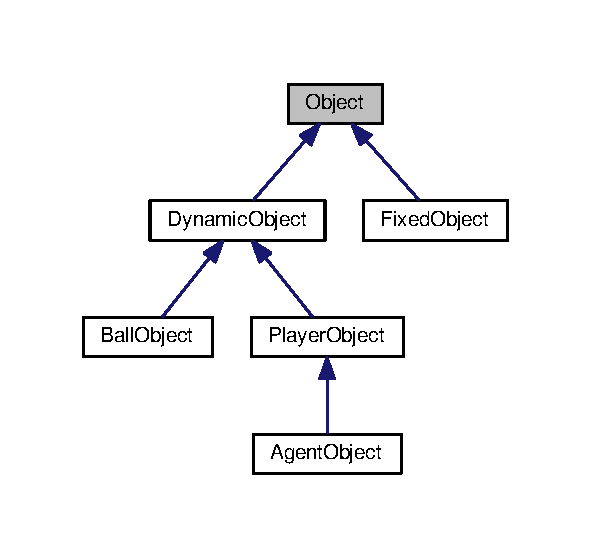
\includegraphics[width=284pt]{classObject__inherit__graph}
\end{center}
\end{figure}


Collaboration diagram for Object\+:
\nopagebreak
\begin{figure}[H]
\begin{center}
\leavevmode
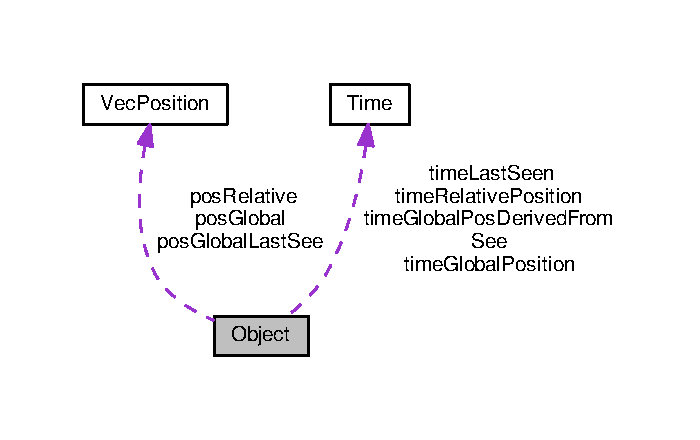
\includegraphics[width=336pt]{classObject__coll__graph}
\end{center}
\end{figure}
\subsection*{Public Member Functions}
\begin{DoxyCompactItemize}
\item 
\hyperlink{classObject_a40860402e64d8008fb42329df7097cdb}{Object} ()
\item 
virtual void \hyperlink{classObject_abdfad2372e7ec5f9aa271a1677653778}{show} (ostream \&os=cout)=0
\item 
\hyperlink{Geometry_8h_a6bfe02ae9bb185092902092561ab2865}{Ang\+Deg} \hyperlink{classObject_a28709fc5998f7f24f3aa32a9dfcd1e42}{get\+Relative\+Angle} ()
\item 
double \hyperlink{classObject_af111de23285de9a9e29f7c7fae6401b6}{get\+Relative\+Distance} ()
\item 
double \hyperlink{classObject_ac2d82f3b7d82f5098095ff83f4af597b}{get\+Confidence} (\hyperlink{classTime}{Time} time)
\item 
bool \hyperlink{classObject_aec36935819c3c4f5050d73a3f2ebbfdb}{set\+Type} (\hyperlink{SoccerTypes_8h_ad4b701fa66e7d26c054ed15b7820c77c}{ObjectT} o)
\item 
\hyperlink{SoccerTypes_8h_ad4b701fa66e7d26c054ed15b7820c77c}{ObjectT} \hyperlink{classObject_a16cba98d16d802e6858a3aee946f7231}{get\+Type} () const 
\item 
bool \hyperlink{classObject_aa31b35b9ee29ee5886e164d19ba461b4}{set\+Relative\+Position} (double d\+Dist, \hyperlink{Geometry_8h_a6bfe02ae9bb185092902092561ab2865}{Ang\+Deg} d\+Ang, \hyperlink{classTime}{Time} time)
\item 
bool \hyperlink{classObject_a1d0f80823f4b2c077a3d91d8ba2b8851}{set\+Relative\+Position} (\hyperlink{classVecPosition}{Vec\+Position} v, \hyperlink{classTime}{Time} time)
\item 
\hyperlink{classVecPosition}{Vec\+Position} \hyperlink{classObject_ac7ecab5852daef8614add5422eb36838}{get\+Relative\+Position} () const 
\item 
bool \hyperlink{classObject_a71656669e4ba8fb84363a33c375c7a83}{set\+Time\+Relative\+Position} (\hyperlink{classTime}{Time} time)
\item 
\hyperlink{classTime}{Time} \hyperlink{classObject_a83fc6b5fe56b15472b9d072bd6cc197b}{get\+Time\+Relative\+Position} () const 
\item 
bool \hyperlink{classObject_aef89da7e4ec7a846b056b8739c486ca4}{set\+Global\+Position} (\hyperlink{classVecPosition}{Vec\+Position} p, \hyperlink{classTime}{Time} time)
\item 
\hyperlink{classVecPosition}{Vec\+Position} \hyperlink{classObject_ac2842396c6a820a0864b767487b465ad}{get\+Global\+Position} () const 
\item 
bool \hyperlink{classObject_a47c32dc89a659bfd381c68ed57917afc}{set\+Time\+Global\+Position} (\hyperlink{classTime}{Time} time)
\item 
\hyperlink{classTime}{Time} \hyperlink{classObject_a599ae480b2d1df43ff83265157a351c1}{get\+Time\+Global\+Position} () const 
\item 
bool \hyperlink{classObject_a65fa38852f3c0ba301dcfa812830c326}{set\+Global\+Position\+Last\+See} (\hyperlink{classVecPosition}{Vec\+Position} p, \hyperlink{classTime}{Time} time)
\item 
\hyperlink{classVecPosition}{Vec\+Position} \hyperlink{classObject_afd7b10a82d0394f1403fc5991a689000}{get\+Global\+Position\+Last\+See} () const 
\item 
bool \hyperlink{classObject_a40b99a05ab37134539b6c52bb95999eb}{set\+Time\+Global\+Pos\+Derived\+From\+See} (\hyperlink{classTime}{Time} time)
\item 
\hyperlink{classTime}{Time} \hyperlink{classObject_abe9fa85b94c18242f856c5c6628077af}{get\+Time\+Global\+Pos\+Derived\+From\+See} () const 
\item 
bool \hyperlink{classObject_a8eedc3dc09c2a67fe6192167f7d2aa60}{set\+Time\+Last\+Seen} (\hyperlink{classTime}{Time} time)
\item 
\hyperlink{classTime}{Time} \hyperlink{classObject_ae2c8eca388d024f1660e203aed3aa35a}{get\+Time\+Last\+Seen} () const 
\end{DoxyCompactItemize}
\subsection*{Protected Attributes}
\begin{DoxyCompactItemize}
\item 
\hyperlink{SoccerTypes_8h_ad4b701fa66e7d26c054ed15b7820c77c}{ObjectT} \hyperlink{classObject_a1ecdca38441a375acbd102de3060b972}{object\+Type}
\item 
\hyperlink{classTime}{Time} \hyperlink{classObject_ac119901c38bac85c71027606f36cd38d}{time\+Last\+Seen}
\item 
\hyperlink{classVecPosition}{Vec\+Position} \hyperlink{classObject_a7b1e09877ae916b49f64b9a9e9a3e0d1}{pos\+Global}
\item 
\hyperlink{classTime}{Time} \hyperlink{classObject_a8892e8727938cdde9c00348848e39b53}{time\+Global\+Position}
\item 
\hyperlink{classVecPosition}{Vec\+Position} \hyperlink{classObject_afc3fa9f935ff0e47ea8057f742ea623c}{pos\+Relative}
\item 
\hyperlink{classTime}{Time} \hyperlink{classObject_a0efe361db316649d7d40132b76ed8d41}{time\+Relative\+Position}
\item 
\hyperlink{classVecPosition}{Vec\+Position} \hyperlink{classObject_a49148cd616efbb888175bfa825dcd167}{pos\+Global\+Last\+See}
\item 
\hyperlink{classTime}{Time} \hyperlink{classObject_a2f113089a45a792db77b03e16b8152a1}{time\+Global\+Pos\+Derived\+From\+See}
\end{DoxyCompactItemize}


\subsection{Detailed Description}
Class \hyperlink{classObject}{Object} contains Robo\+Cup information that is available for all objects in the simulation. All (relative) information is relative to an agent as declared in \hyperlink{classAgentObject}{Agent\+Object}. Update of an object (or one of the subclasses) happens by calling the standard get and set methods available in these classes. Calculations on these attributes do not occur in these classes, but in the update methods of the \hyperlink{classWorldModel}{World\+Model}. 

\subsection{Constructor \& Destructor Documentation}
\index{Object@{Object}!Object@{Object}}
\index{Object@{Object}!Object@{Object}}
\subsubsection[{\texorpdfstring{Object()}{Object()}}]{\setlength{\rightskip}{0pt plus 5cm}Object\+::\+Object (
\begin{DoxyParamCaption}
{}
\end{DoxyParamCaption}
)}\hypertarget{classObject_a40860402e64d8008fb42329df7097cdb}{}\label{classObject_a40860402e64d8008fb42329df7097cdb}
This constructor creates an object, all variables are initialized by default (illegal) values 

\subsection{Member Function Documentation}
\index{Object@{Object}!get\+Confidence@{get\+Confidence}}
\index{get\+Confidence@{get\+Confidence}!Object@{Object}}
\subsubsection[{\texorpdfstring{get\+Confidence(\+Time time)}{getConfidence(Time time)}}]{\setlength{\rightskip}{0pt plus 5cm}double Object\+::get\+Confidence (
\begin{DoxyParamCaption}
\item[{{\bf Time}}]{time}
\end{DoxyParamCaption}
)}\hypertarget{classObject_ac2d82f3b7d82f5098095ff83f4af597b}{}\label{classObject_ac2d82f3b7d82f5098095ff83f4af597b}
This method returns the confidence of the information of this object. The confidence is related to the last time this object was seen and the specified time (normally the time of the last received message). 
\begin{DoxyParams}{Parameters}
{\em time} & current time to compare with time object was last seen \\
\hline
\end{DoxyParams}
\begin{DoxyReturn}{Returns}
confidence factor of this object 
\end{DoxyReturn}
\index{Object@{Object}!get\+Global\+Position@{get\+Global\+Position}}
\index{get\+Global\+Position@{get\+Global\+Position}!Object@{Object}}
\subsubsection[{\texorpdfstring{get\+Global\+Position() const }{getGlobalPosition() const }}]{\setlength{\rightskip}{0pt plus 5cm}{\bf Vec\+Position} Object\+::get\+Global\+Position (
\begin{DoxyParamCaption}
{}
\end{DoxyParamCaption}
) const}\hypertarget{classObject_ac2842396c6a820a0864b767487b465ad}{}\label{classObject_ac2842396c6a820a0864b767487b465ad}
This method returns the global position of this object. The time of this information is related to the time returned by \hyperlink{classObject_a599ae480b2d1df43ff83265157a351c1}{get\+Time\+Global\+Position()}, but is not checked. So if you want to know the relevance of this position use this method. \begin{DoxyReturn}{Returns}
global position of this object 
\end{DoxyReturn}
\index{Object@{Object}!get\+Global\+Position\+Last\+See@{get\+Global\+Position\+Last\+See}}
\index{get\+Global\+Position\+Last\+See@{get\+Global\+Position\+Last\+See}!Object@{Object}}
\subsubsection[{\texorpdfstring{get\+Global\+Position\+Last\+See() const }{getGlobalPositionLastSee() const }}]{\setlength{\rightskip}{0pt plus 5cm}{\bf Vec\+Position} Object\+::get\+Global\+Position\+Last\+See (
\begin{DoxyParamCaption}
{}
\end{DoxyParamCaption}
) const}\hypertarget{classObject_afd7b10a82d0394f1403fc5991a689000}{}\label{classObject_afd7b10a82d0394f1403fc5991a689000}
This method returns the global position of this object at the time of the last see message. The time of this information is related to the time returned by \hyperlink{classObject_abe9fa85b94c18242f856c5c6628077af}{get\+Time\+Global\+Pos\+Derived\+From\+See()}. \begin{DoxyReturn}{Returns}
global position of this object 
\end{DoxyReturn}
\index{Object@{Object}!get\+Relative\+Angle@{get\+Relative\+Angle}}
\index{get\+Relative\+Angle@{get\+Relative\+Angle}!Object@{Object}}
\subsubsection[{\texorpdfstring{get\+Relative\+Angle()}{getRelativeAngle()}}]{\setlength{\rightskip}{0pt plus 5cm}{\bf Ang\+Deg} Object\+::get\+Relative\+Angle (
\begin{DoxyParamCaption}
{}
\end{DoxyParamCaption}
)}\hypertarget{classObject_a28709fc5998f7f24f3aa32a9dfcd1e42}{}\label{classObject_a28709fc5998f7f24f3aa32a9dfcd1e42}
This method returns the relative angle of this object to the agent. This equals the angle of the relative position vector. \begin{DoxyReturn}{Returns}
relative angle to this object 
\end{DoxyReturn}
\index{Object@{Object}!get\+Relative\+Distance@{get\+Relative\+Distance}}
\index{get\+Relative\+Distance@{get\+Relative\+Distance}!Object@{Object}}
\subsubsection[{\texorpdfstring{get\+Relative\+Distance()}{getRelativeDistance()}}]{\setlength{\rightskip}{0pt plus 5cm}double Object\+::get\+Relative\+Distance (
\begin{DoxyParamCaption}
{}
\end{DoxyParamCaption}
)}\hypertarget{classObject_af111de23285de9a9e29f7c7fae6401b6}{}\label{classObject_af111de23285de9a9e29f7c7fae6401b6}
This method returns the relative distance to this object. This equals the magnitude of the relative position vector. \begin{DoxyReturn}{Returns}
relative distance to this object 
\end{DoxyReturn}
\index{Object@{Object}!get\+Relative\+Position@{get\+Relative\+Position}}
\index{get\+Relative\+Position@{get\+Relative\+Position}!Object@{Object}}
\subsubsection[{\texorpdfstring{get\+Relative\+Position() const }{getRelativePosition() const }}]{\setlength{\rightskip}{0pt plus 5cm}{\bf Vec\+Position} Object\+::get\+Relative\+Position (
\begin{DoxyParamCaption}
{}
\end{DoxyParamCaption}
) const}\hypertarget{classObject_ac7ecab5852daef8614add5422eb36838}{}\label{classObject_ac7ecab5852daef8614add5422eb36838}
This method returns the relative position of this object. The time of this information is related to the time returned by \hyperlink{classObject_a83fc6b5fe56b15472b9d072bd6cc197b}{get\+Time\+Relative\+Position()}, but is not checked. So if you want to know the relevance of this position use this method. \begin{DoxyReturn}{Returns}
relative position of this object 
\end{DoxyReturn}
\index{Object@{Object}!get\+Time\+Global\+Pos\+Derived\+From\+See@{get\+Time\+Global\+Pos\+Derived\+From\+See}}
\index{get\+Time\+Global\+Pos\+Derived\+From\+See@{get\+Time\+Global\+Pos\+Derived\+From\+See}!Object@{Object}}
\subsubsection[{\texorpdfstring{get\+Time\+Global\+Pos\+Derived\+From\+See() const }{getTimeGlobalPosDerivedFromSee() const }}]{\setlength{\rightskip}{0pt plus 5cm}{\bf Time} Object\+::get\+Time\+Global\+Pos\+Derived\+From\+See (
\begin{DoxyParamCaption}
{}
\end{DoxyParamCaption}
) const}\hypertarget{classObject_abe9fa85b94c18242f856c5c6628077af}{}\label{classObject_abe9fa85b94c18242f856c5c6628077af}
This method returns the time that the global position was calculated using a see message. \begin{DoxyReturn}{Returns}
time of the global position of this object during the last see 
\end{DoxyReturn}
\index{Object@{Object}!get\+Time\+Global\+Position@{get\+Time\+Global\+Position}}
\index{get\+Time\+Global\+Position@{get\+Time\+Global\+Position}!Object@{Object}}
\subsubsection[{\texorpdfstring{get\+Time\+Global\+Position() const }{getTimeGlobalPosition() const }}]{\setlength{\rightskip}{0pt plus 5cm}{\bf Time} Object\+::get\+Time\+Global\+Position (
\begin{DoxyParamCaption}
{}
\end{DoxyParamCaption}
) const}\hypertarget{classObject_a599ae480b2d1df43ff83265157a351c1}{}\label{classObject_a599ae480b2d1df43ff83265157a351c1}
This method returns the time that corresponds to the global position of this object. \begin{DoxyReturn}{Returns}
time of the global position of this object 
\end{DoxyReturn}
\index{Object@{Object}!get\+Time\+Last\+Seen@{get\+Time\+Last\+Seen}}
\index{get\+Time\+Last\+Seen@{get\+Time\+Last\+Seen}!Object@{Object}}
\subsubsection[{\texorpdfstring{get\+Time\+Last\+Seen() const }{getTimeLastSeen() const }}]{\setlength{\rightskip}{0pt plus 5cm}{\bf Time} Object\+::get\+Time\+Last\+Seen (
\begin{DoxyParamCaption}
{}
\end{DoxyParamCaption}
) const}\hypertarget{classObject_ae2c8eca388d024f1660e203aed3aa35a}{}\label{classObject_ae2c8eca388d024f1660e203aed3aa35a}
This method returns the time that corresponds to the time this object was located in the last see message. \begin{DoxyReturn}{Returns}
time of the last see message that was used to update this object 
\end{DoxyReturn}
\index{Object@{Object}!get\+Time\+Relative\+Position@{get\+Time\+Relative\+Position}}
\index{get\+Time\+Relative\+Position@{get\+Time\+Relative\+Position}!Object@{Object}}
\subsubsection[{\texorpdfstring{get\+Time\+Relative\+Position() const }{getTimeRelativePosition() const }}]{\setlength{\rightskip}{0pt plus 5cm}{\bf Time} Object\+::get\+Time\+Relative\+Position (
\begin{DoxyParamCaption}
{}
\end{DoxyParamCaption}
) const}\hypertarget{classObject_a83fc6b5fe56b15472b9d072bd6cc197b}{}\label{classObject_a83fc6b5fe56b15472b9d072bd6cc197b}
This method returns the time that corresponds to the relative position of this object. \begin{DoxyReturn}{Returns}
time of the relative position of this object 
\end{DoxyReturn}
\index{Object@{Object}!get\+Type@{get\+Type}}
\index{get\+Type@{get\+Type}!Object@{Object}}
\subsubsection[{\texorpdfstring{get\+Type() const }{getType() const }}]{\setlength{\rightskip}{0pt plus 5cm}{\bf ObjectT} Object\+::get\+Type (
\begin{DoxyParamCaption}
{}
\end{DoxyParamCaption}
) const}\hypertarget{classObject_a16cba98d16d802e6858a3aee946f7231}{}\label{classObject_a16cba98d16d802e6858a3aee946f7231}
This method returns the type of this object. \begin{DoxyReturn}{Returns}
type of this object 
\end{DoxyReturn}
\index{Object@{Object}!set\+Global\+Position@{set\+Global\+Position}}
\index{set\+Global\+Position@{set\+Global\+Position}!Object@{Object}}
\subsubsection[{\texorpdfstring{set\+Global\+Position(\+Vec\+Position p, Time time)}{setGlobalPosition(VecPosition p, Time time)}}]{\setlength{\rightskip}{0pt plus 5cm}bool Object\+::set\+Global\+Position (
\begin{DoxyParamCaption}
\item[{{\bf Vec\+Position}}]{p, }
\item[{{\bf Time}}]{time}
\end{DoxyParamCaption}
)}\hypertarget{classObject_aef89da7e4ec7a846b056b8739c486ca4}{}\label{classObject_aef89da7e4ec7a846b056b8739c486ca4}
This method sets the global position and the time this information was calculated. 
\begin{DoxyParams}{Parameters}
{\em p} & new global position \\
\hline
{\em time} & time global position was received \\
\hline
\end{DoxyParams}
\begin{DoxyReturn}{Returns}
bool indicating whether the values were set 
\end{DoxyReturn}
\index{Object@{Object}!set\+Global\+Position\+Last\+See@{set\+Global\+Position\+Last\+See}}
\index{set\+Global\+Position\+Last\+See@{set\+Global\+Position\+Last\+See}!Object@{Object}}
\subsubsection[{\texorpdfstring{set\+Global\+Position\+Last\+See(\+Vec\+Position p, Time time)}{setGlobalPositionLastSee(VecPosition p, Time time)}}]{\setlength{\rightskip}{0pt plus 5cm}bool Object\+::set\+Global\+Position\+Last\+See (
\begin{DoxyParamCaption}
\item[{{\bf Vec\+Position}}]{p, }
\item[{{\bf Time}}]{time}
\end{DoxyParamCaption}
)}\hypertarget{classObject_a65fa38852f3c0ba301dcfa812830c326}{}\label{classObject_a65fa38852f3c0ba301dcfa812830c326}
This method sets the global position calculated using the last see message and the time of this see message. This opposed to the \char`\"{}normal\char`\"{} global position that is also updated when no see message has arrived in a new cycle. 
\begin{DoxyParams}{Parameters}
{\em p} & new global position \\
\hline
{\em time} & time global position was received \\
\hline
\end{DoxyParams}
\begin{DoxyReturn}{Returns}
bool indicating whether the values were set 
\end{DoxyReturn}
\index{Object@{Object}!set\+Relative\+Position@{set\+Relative\+Position}}
\index{set\+Relative\+Position@{set\+Relative\+Position}!Object@{Object}}
\subsubsection[{\texorpdfstring{set\+Relative\+Position(double d\+Dist, Ang\+Deg d\+Ang, Time time)}{setRelativePosition(double dDist, AngDeg dAng, Time time)}}]{\setlength{\rightskip}{0pt plus 5cm}bool Object\+::set\+Relative\+Position (
\begin{DoxyParamCaption}
\item[{double}]{d\+Dist, }
\item[{{\bf Ang\+Deg}}]{ang, }
\item[{{\bf Time}}]{time}
\end{DoxyParamCaption}
)}\hypertarget{classObject_aa31b35b9ee29ee5886e164d19ba461b4}{}\label{classObject_aa31b35b9ee29ee5886e164d19ba461b4}
This method sets the relative position and the time this information was received. The relative position is calculated using the given distance and the given (relative) angle. 
\begin{DoxyParams}{Parameters}
{\em d\+Dist} & relative distance to object \\
\hline
{\em ang} & relative angle to object \\
\hline
{\em time} & time relative position was received \\
\hline
\end{DoxyParams}
\begin{DoxyReturn}{Returns}
bool indicating whether the values were set 
\end{DoxyReturn}
\index{Object@{Object}!set\+Relative\+Position@{set\+Relative\+Position}}
\index{set\+Relative\+Position@{set\+Relative\+Position}!Object@{Object}}
\subsubsection[{\texorpdfstring{set\+Relative\+Position(\+Vec\+Position v, Time time)}{setRelativePosition(VecPosition v, Time time)}}]{\setlength{\rightskip}{0pt plus 5cm}bool Object\+::set\+Relative\+Position (
\begin{DoxyParamCaption}
\item[{{\bf Vec\+Position}}]{v, }
\item[{{\bf Time}}]{time}
\end{DoxyParamCaption}
)}\hypertarget{classObject_a1d0f80823f4b2c077a3d91d8ba2b8851}{}\label{classObject_a1d0f80823f4b2c077a3d91d8ba2b8851}
This method sets the relative position and the time this information was received using a vec\+Position. 
\begin{DoxyParams}{Parameters}
{\em p} & new relative position \\
\hline
{\em time} & time relative position was received \\
\hline
\end{DoxyParams}
\begin{DoxyReturn}{Returns}
bool indicating whether the values were set 
\end{DoxyReturn}
\index{Object@{Object}!set\+Time\+Global\+Pos\+Derived\+From\+See@{set\+Time\+Global\+Pos\+Derived\+From\+See}}
\index{set\+Time\+Global\+Pos\+Derived\+From\+See@{set\+Time\+Global\+Pos\+Derived\+From\+See}!Object@{Object}}
\subsubsection[{\texorpdfstring{set\+Time\+Global\+Pos\+Derived\+From\+See(\+Time time)}{setTimeGlobalPosDerivedFromSee(Time time)}}]{\setlength{\rightskip}{0pt plus 5cm}bool Object\+::set\+Time\+Global\+Pos\+Derived\+From\+See (
\begin{DoxyParamCaption}
\item[{{\bf Time}}]{time}
\end{DoxyParamCaption}
)}\hypertarget{classObject_a40b99a05ab37134539b6c52bb95999eb}{}\label{classObject_a40b99a05ab37134539b6c52bb95999eb}
This method sets the time the global position was calculated using a see message. 
\begin{DoxyParams}{Parameters}
{\em time} & time global position was calculated with see message \\
\hline
\end{DoxyParams}
\begin{DoxyReturn}{Returns}
bool indicating whether the value was set 
\end{DoxyReturn}
\index{Object@{Object}!set\+Time\+Global\+Position@{set\+Time\+Global\+Position}}
\index{set\+Time\+Global\+Position@{set\+Time\+Global\+Position}!Object@{Object}}
\subsubsection[{\texorpdfstring{set\+Time\+Global\+Position(\+Time time)}{setTimeGlobalPosition(Time time)}}]{\setlength{\rightskip}{0pt plus 5cm}bool Object\+::set\+Time\+Global\+Position (
\begin{DoxyParamCaption}
\item[{{\bf Time}}]{time}
\end{DoxyParamCaption}
)}\hypertarget{classObject_a47c32dc89a659bfd381c68ed57917afc}{}\label{classObject_a47c32dc89a659bfd381c68ed57917afc}
This method sets the time the global position was calculated 
\begin{DoxyParams}{Parameters}
{\em time} & time global position was calculated \\
\hline
\end{DoxyParams}
\begin{DoxyReturn}{Returns}
bool indicating whether the value was set 
\end{DoxyReturn}
\index{Object@{Object}!set\+Time\+Last\+Seen@{set\+Time\+Last\+Seen}}
\index{set\+Time\+Last\+Seen@{set\+Time\+Last\+Seen}!Object@{Object}}
\subsubsection[{\texorpdfstring{set\+Time\+Last\+Seen(\+Time time)}{setTimeLastSeen(Time time)}}]{\setlength{\rightskip}{0pt plus 5cm}bool Object\+::set\+Time\+Last\+Seen (
\begin{DoxyParamCaption}
\item[{{\bf Time}}]{time}
\end{DoxyParamCaption}
)}\hypertarget{classObject_a8eedc3dc09c2a67fe6192167f7d2aa60}{}\label{classObject_a8eedc3dc09c2a67fe6192167f7d2aa60}
This method sets the time of the last see message in which this object was seen. 
\begin{DoxyParams}{Parameters}
{\em time} & time this object was last seen \\
\hline
\end{DoxyParams}
\begin{DoxyReturn}{Returns}
bool indicating whether the value was set 
\end{DoxyReturn}
\index{Object@{Object}!set\+Time\+Relative\+Position@{set\+Time\+Relative\+Position}}
\index{set\+Time\+Relative\+Position@{set\+Time\+Relative\+Position}!Object@{Object}}
\subsubsection[{\texorpdfstring{set\+Time\+Relative\+Position(\+Time time)}{setTimeRelativePosition(Time time)}}]{\setlength{\rightskip}{0pt plus 5cm}bool Object\+::set\+Time\+Relative\+Position (
\begin{DoxyParamCaption}
\item[{{\bf Time}}]{time}
\end{DoxyParamCaption}
)}\hypertarget{classObject_a71656669e4ba8fb84363a33c375c7a83}{}\label{classObject_a71656669e4ba8fb84363a33c375c7a83}
This method sets the time the relative position was received. 
\begin{DoxyParams}{Parameters}
{\em time} & time relative position was received \\
\hline
\end{DoxyParams}
\begin{DoxyReturn}{Returns}
bool indicating whether the value was set 
\end{DoxyReturn}
\index{Object@{Object}!set\+Type@{set\+Type}}
\index{set\+Type@{set\+Type}!Object@{Object}}
\subsubsection[{\texorpdfstring{set\+Type(\+Object\+T o)}{setType(ObjectT o)}}]{\setlength{\rightskip}{0pt plus 5cm}bool Object\+::set\+Type (
\begin{DoxyParamCaption}
\item[{{\bf ObjectT}}]{o}
\end{DoxyParamCaption}
)}\hypertarget{classObject_aec36935819c3c4f5050d73a3f2ebbfdb}{}\label{classObject_aec36935819c3c4f5050d73a3f2ebbfdb}
This method sets the type of this object (i.\+e. O\+B\+J\+E\+C\+T\+\_\+\+B\+A\+LL, F\+L\+A\+G\+\_\+\+L\+\_\+\+R\+\_\+T). 
\begin{DoxyParams}{Parameters}
{\em o} & ObjectT representing the type of this object \\
\hline
\end{DoxyParams}
\begin{DoxyReturn}{Returns}
bool indicating whether value was set. 
\end{DoxyReturn}
\index{Object@{Object}!show@{show}}
\index{show@{show}!Object@{Object}}
\subsubsection[{\texorpdfstring{show(ostream \&os=cout)=0}{show(ostream &os=cout)=0}}]{\setlength{\rightskip}{0pt plus 5cm}virtual void Object\+::show (
\begin{DoxyParamCaption}
\item[{ostream \&}]{os = {\ttfamily cout}}
\end{DoxyParamCaption}
)\hspace{0.3cm}{\ttfamily [pure virtual]}}\hypertarget{classObject_abdfad2372e7ec5f9aa271a1677653778}{}\label{classObject_abdfad2372e7ec5f9aa271a1677653778}
abstract function that should be defined in a subclass 

Implemented in \hyperlink{classAgentObject_a0043cea8d237828930412eb3c2b84e32}{Agent\+Object}, \hyperlink{classBallObject_a294d8fb34c88d98a1ef2ed2d1c864a62}{Ball\+Object}, \hyperlink{classPlayerObject_a01d587f88139dddf2ca1b39a65523dd6}{Player\+Object}, and \hyperlink{classFixedObject_ad8771b36cc2073d4a9fe1879b2f91d06}{Fixed\+Object}.



\subsection{Member Data Documentation}
\index{Object@{Object}!object\+Type@{object\+Type}}
\index{object\+Type@{object\+Type}!Object@{Object}}
\subsubsection[{\texorpdfstring{object\+Type}{objectType}}]{\setlength{\rightskip}{0pt plus 5cm}{\bf ObjectT} Object\+::object\+Type\hspace{0.3cm}{\ttfamily [protected]}}\hypertarget{classObject_a1ecdca38441a375acbd102de3060b972}{}\label{classObject_a1ecdca38441a375acbd102de3060b972}
Type of this object \index{Object@{Object}!pos\+Global@{pos\+Global}}
\index{pos\+Global@{pos\+Global}!Object@{Object}}
\subsubsection[{\texorpdfstring{pos\+Global}{posGlobal}}]{\setlength{\rightskip}{0pt plus 5cm}{\bf Vec\+Position} Object\+::pos\+Global\hspace{0.3cm}{\ttfamily [protected]}}\hypertarget{classObject_a7b1e09877ae916b49f64b9a9e9a3e0d1}{}\label{classObject_a7b1e09877ae916b49f64b9a9e9a3e0d1}
Global position in the field \index{Object@{Object}!pos\+Global\+Last\+See@{pos\+Global\+Last\+See}}
\index{pos\+Global\+Last\+See@{pos\+Global\+Last\+See}!Object@{Object}}
\subsubsection[{\texorpdfstring{pos\+Global\+Last\+See}{posGlobalLastSee}}]{\setlength{\rightskip}{0pt plus 5cm}{\bf Vec\+Position} Object\+::pos\+Global\+Last\+See\hspace{0.3cm}{\ttfamily [protected]}}\hypertarget{classObject_a49148cd616efbb888175bfa825dcd167}{}\label{classObject_a49148cd616efbb888175bfa825dcd167}
Global position of last see msg \index{Object@{Object}!pos\+Relative@{pos\+Relative}}
\index{pos\+Relative@{pos\+Relative}!Object@{Object}}
\subsubsection[{\texorpdfstring{pos\+Relative}{posRelative}}]{\setlength{\rightskip}{0pt plus 5cm}{\bf Vec\+Position} Object\+::pos\+Relative\hspace{0.3cm}{\ttfamily [protected]}}\hypertarget{classObject_afc3fa9f935ff0e47ea8057f742ea623c}{}\label{classObject_afc3fa9f935ff0e47ea8057f742ea623c}
Relative position of the object \index{Object@{Object}!time\+Global\+Pos\+Derived\+From\+See@{time\+Global\+Pos\+Derived\+From\+See}}
\index{time\+Global\+Pos\+Derived\+From\+See@{time\+Global\+Pos\+Derived\+From\+See}!Object@{Object}}
\subsubsection[{\texorpdfstring{time\+Global\+Pos\+Derived\+From\+See}{timeGlobalPosDerivedFromSee}}]{\setlength{\rightskip}{0pt plus 5cm}{\bf Time} Object\+::time\+Global\+Pos\+Derived\+From\+See\hspace{0.3cm}{\ttfamily [protected]}}\hypertarget{classObject_a2f113089a45a792db77b03e16b8152a1}{}\label{classObject_a2f113089a45a792db77b03e16b8152a1}
\hyperlink{classTime}{Time} pos derived from see msg \index{Object@{Object}!time\+Global\+Position@{time\+Global\+Position}}
\index{time\+Global\+Position@{time\+Global\+Position}!Object@{Object}}
\subsubsection[{\texorpdfstring{time\+Global\+Position}{timeGlobalPosition}}]{\setlength{\rightskip}{0pt plus 5cm}{\bf Time} Object\+::time\+Global\+Position\hspace{0.3cm}{\ttfamily [protected]}}\hypertarget{classObject_a8892e8727938cdde9c00348848e39b53}{}\label{classObject_a8892e8727938cdde9c00348848e39b53}
Server time of global position \index{Object@{Object}!time\+Last\+Seen@{time\+Last\+Seen}}
\index{time\+Last\+Seen@{time\+Last\+Seen}!Object@{Object}}
\subsubsection[{\texorpdfstring{time\+Last\+Seen}{timeLastSeen}}]{\setlength{\rightskip}{0pt plus 5cm}{\bf Time} Object\+::time\+Last\+Seen\hspace{0.3cm}{\ttfamily [protected]}}\hypertarget{classObject_ac119901c38bac85c71027606f36cd38d}{}\label{classObject_ac119901c38bac85c71027606f36cd38d}
\hyperlink{classTime}{Time} last see message has arrived \index{Object@{Object}!time\+Relative\+Position@{time\+Relative\+Position}}
\index{time\+Relative\+Position@{time\+Relative\+Position}!Object@{Object}}
\subsubsection[{\texorpdfstring{time\+Relative\+Position}{timeRelativePosition}}]{\setlength{\rightskip}{0pt plus 5cm}{\bf Time} Object\+::time\+Relative\+Position\hspace{0.3cm}{\ttfamily [protected]}}\hypertarget{classObject_a0efe361db316649d7d40132b76ed8d41}{}\label{classObject_a0efe361db316649d7d40132b76ed8d41}
Server time of relative position 

The documentation for this class was generated from the following files\+:\begin{DoxyCompactItemize}
\item 
src/\hyperlink{Objects_8h}{Objects.\+h}\item 
src/\hyperlink{Objects_8cpp}{Objects.\+cpp}\end{DoxyCompactItemize}

\hypertarget{classParse}{}\section{Parse Class Reference}
\label{classParse}\index{Parse@{Parse}}


{\ttfamily \#include $<$Parse.\+h$>$}

\subsection*{Static Public Member Functions}
\begin{DoxyCompactItemize}
\item 
static double \hyperlink{classParse_abb2c6feb8d0f3aa33fc65456b52c2996}{parse\+First\+Double} (char $\ast$$\ast$str\+Msg)
\item 
static int \hyperlink{classParse_ad7ff96efeada853f0d4c51e5344e6edb}{parse\+First\+Int} (char $\ast$$\ast$str\+Msg)
\item 
static char \hyperlink{classParse_ad77357913848f872385f44ec531526d0}{goto\+First\+Space\+Or\+Closing\+Bracket} (char $\ast$$\ast$str\+Msg)
\item 
static int \hyperlink{classParse_a2f02549c9c6b0de82e38ce5b12654b54}{goto\+First\+Occurence\+Of} (char c, char $\ast$$\ast$str\+Msg)
\item 
static char \hyperlink{classParse_a20b93ee95332798ad4947f4a898320ca}{goto\+First\+Non\+Space} (char $\ast$$\ast$str\+Msg)
\end{DoxyCompactItemize}


\subsection{Detailed Description}
This class contains several static methods which can be used for parsing string messages and uses some of the ideas contained in C\+MU\textquotesingle{}99 source code of Peter Stone. Tests shows that scanning integers has a performance increase of 30.\+3\% over the method used by C\+M\+United and 68.\+0\% over sscanf. For parsing doubles the performance increase was 15.\+4\% compared to C\+M\+United and 85.\+1\% compared to sscanf. 

\subsection{Member Function Documentation}
\index{Parse@{Parse}!goto\+First\+Non\+Space@{goto\+First\+Non\+Space}}
\index{goto\+First\+Non\+Space@{goto\+First\+Non\+Space}!Parse@{Parse}}
\subsubsection[{\texorpdfstring{goto\+First\+Non\+Space(char $\ast$$\ast$str\+Msg)}{gotoFirstNonSpace(char **strMsg)}}]{\setlength{\rightskip}{0pt plus 5cm}char Parse\+::goto\+First\+Non\+Space (
\begin{DoxyParamCaption}
\item[{char $\ast$$\ast$}]{str\+Msg}
\end{DoxyParamCaption}
)\hspace{0.3cm}{\ttfamily [static]}}\hypertarget{classParse_a20b93ee95332798ad4947f4a898320ca}{}\label{classParse_a20b93ee95332798ad4947f4a898320ca}
This method walks through the string starting at the character where str\+Msg points to and stops when or the end of the string is reached or a non space is reached. str\+Msg is updated to this new position. 
\begin{DoxyParams}{Parameters}
{\em str\+Msg} & pointer to a character in a string array \\
\hline
\end{DoxyParams}
\begin{DoxyReturn}{Returns}
character that is at the first non space, \textquotesingle{}\textbackslash{}0\textquotesingle{} when end of string is reached. 
\end{DoxyReturn}
\index{Parse@{Parse}!goto\+First\+Occurence\+Of@{goto\+First\+Occurence\+Of}}
\index{goto\+First\+Occurence\+Of@{goto\+First\+Occurence\+Of}!Parse@{Parse}}
\subsubsection[{\texorpdfstring{goto\+First\+Occurence\+Of(char c, char $\ast$$\ast$str\+Msg)}{gotoFirstOccurenceOf(char c, char **strMsg)}}]{\setlength{\rightskip}{0pt plus 5cm}int Parse\+::goto\+First\+Occurence\+Of (
\begin{DoxyParamCaption}
\item[{char}]{c, }
\item[{char $\ast$$\ast$}]{str\+Msg}
\end{DoxyParamCaption}
)\hspace{0.3cm}{\ttfamily [static]}}\hypertarget{classParse_a2f02549c9c6b0de82e38ce5b12654b54}{}\label{classParse_a2f02549c9c6b0de82e38ce5b12654b54}
This method walks through the string starting at the character where str\+Msg points to and stops when the character c is reached. str\+Msg is changed after this method is called.. 
\begin{DoxyParams}{Parameters}
{\em c} & character that is searched for in str\+Msg. \\
\hline
{\em str\+Msg} & pointer to a character in a string array \\
\hline
\end{DoxyParams}
\begin{DoxyReturn}{Returns}
number of character skipped to reach c, -\/1 when not found 
\end{DoxyReturn}
\index{Parse@{Parse}!goto\+First\+Space\+Or\+Closing\+Bracket@{goto\+First\+Space\+Or\+Closing\+Bracket}}
\index{goto\+First\+Space\+Or\+Closing\+Bracket@{goto\+First\+Space\+Or\+Closing\+Bracket}!Parse@{Parse}}
\subsubsection[{\texorpdfstring{goto\+First\+Space\+Or\+Closing\+Bracket(char $\ast$$\ast$str\+Msg)}{gotoFirstSpaceOrClosingBracket(char **strMsg)}}]{\setlength{\rightskip}{0pt plus 5cm}char Parse\+::goto\+First\+Space\+Or\+Closing\+Bracket (
\begin{DoxyParamCaption}
\item[{char $\ast$$\ast$}]{str\+Msg}
\end{DoxyParamCaption}
)\hspace{0.3cm}{\ttfamily [static]}}\hypertarget{classParse_ad77357913848f872385f44ec531526d0}{}\label{classParse_ad77357913848f872385f44ec531526d0}
This method walks through the string starting at the character where str\+Msg points to and stops when~\newline

\begin{DoxyItemize}
\item the end of the string is reached~\newline

\item a character different than \textquotesingle{} \textquotesingle{} and \textquotesingle{})\textquotesingle{} is read~\newline
 str\+Msg is changed after this method is called. 
\begin{DoxyParams}{Parameters}
{\em str\+Msg} & pointer to a character in a string array \\
\hline
\end{DoxyParams}
\begin{DoxyReturn}{Returns}
first character that is not equal to \textquotesingle{} \textquotesingle{} or \textquotesingle{})\textquotesingle{}, \textquotesingle{}\textbackslash{}0\textquotesingle{} when string didn\textquotesingle{}t contain such a character. 
\end{DoxyReturn}

\end{DoxyItemize}\index{Parse@{Parse}!parse\+First\+Double@{parse\+First\+Double}}
\index{parse\+First\+Double@{parse\+First\+Double}!Parse@{Parse}}
\subsubsection[{\texorpdfstring{parse\+First\+Double(char $\ast$$\ast$str\+Msg)}{parseFirstDouble(char **strMsg)}}]{\setlength{\rightskip}{0pt plus 5cm}double Parse\+::parse\+First\+Double (
\begin{DoxyParamCaption}
\item[{char $\ast$$\ast$}]{str\+Msg}
\end{DoxyParamCaption}
)\hspace{0.3cm}{\ttfamily [static]}}\hypertarget{classParse_abb2c6feb8d0f3aa33fc65456b52c2996}{}\label{classParse_abb2c6feb8d0f3aa33fc65456b52c2996}
This method walks through the string starting at the character where str\+Msg points to and returns the first double that can be read from this string. Any other characters in front of this integer are discarded. After this method is returned, str\+Msg points to the first character after the final value of the double. 4e-\/3, and NaN or nan are also recognized. When input contains NaN or nan, -\/1000.\+0 is returned. 
\begin{DoxyParams}{Parameters}
{\em str\+Msg} & pointer to a character in a string array \\
\hline
\end{DoxyParams}
\begin{DoxyReturn}{Returns}
first double that can be read from this string. 
\end{DoxyReturn}
\index{Parse@{Parse}!parse\+First\+Int@{parse\+First\+Int}}
\index{parse\+First\+Int@{parse\+First\+Int}!Parse@{Parse}}
\subsubsection[{\texorpdfstring{parse\+First\+Int(char $\ast$$\ast$str\+Msg)}{parseFirstInt(char **strMsg)}}]{\setlength{\rightskip}{0pt plus 5cm}int Parse\+::parse\+First\+Int (
\begin{DoxyParamCaption}
\item[{char $\ast$$\ast$}]{str\+Msg}
\end{DoxyParamCaption}
)\hspace{0.3cm}{\ttfamily [static]}}\hypertarget{classParse_ad7ff96efeada853f0d4c51e5344e6edb}{}\label{classParse_ad7ff96efeada853f0d4c51e5344e6edb}
This method walks through the string starting at the character where str\+Msg points to and returns the first integer that can be read from this string. Any other characters in front of this integer are discarded. After this method is returned, str\+Msg points to the first character after the final value of the integer. 
\begin{DoxyParams}{Parameters}
{\em str\+Msg} & pointer to a character in a string array \\
\hline
\end{DoxyParams}
\begin{DoxyReturn}{Returns}
first integer that can be read from this string. 
\end{DoxyReturn}


The documentation for this class was generated from the following files\+:\begin{DoxyCompactItemize}
\item 
src/\hyperlink{Parse_8h}{Parse.\+h}\item 
src/\hyperlink{Parse_8cpp}{Parse.\+cpp}\end{DoxyCompactItemize}

\hypertarget{classPlayer}{}\section{Player Class Reference}
\label{classPlayer}\index{Player@{Player}}


{\ttfamily \#include $<$Player.\+h$>$}



Inheritance diagram for Player\+:
\nopagebreak
\begin{figure}[H]
\begin{center}
\leavevmode
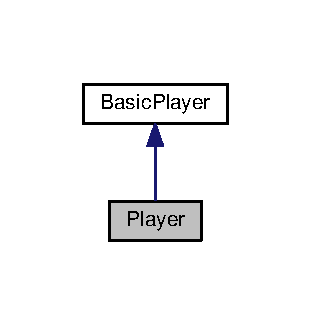
\includegraphics[width=149pt]{classPlayer__inherit__graph}
\end{center}
\end{figure}


Collaboration diagram for Player\+:
\nopagebreak
\begin{figure}[H]
\begin{center}
\leavevmode
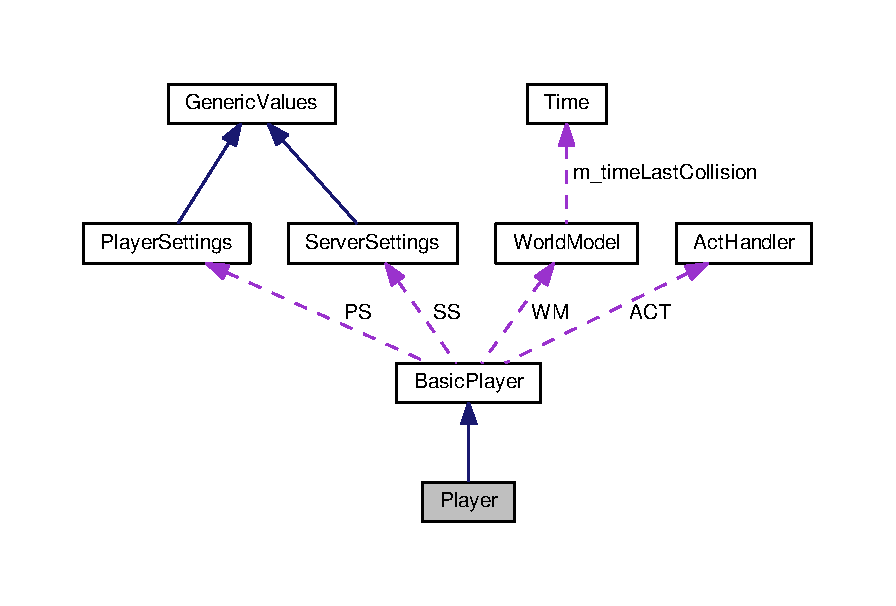
\includegraphics[width=350pt]{classPlayer__coll__graph}
\end{center}
\end{figure}
\subsection*{Public Member Functions}
\begin{DoxyCompactItemize}
\item 
\hyperlink{classPlayer_a4c153178edd52d55138de2b29bfe8b4e}{Player} (\hyperlink{classActHandler}{Act\+Handler} $\ast$a, \hyperlink{classWorldModel}{World\+Model} $\ast$wm, \hyperlink{classServerSettings}{Server\+Settings} $\ast$ss, \hyperlink{classPlayerSettings}{Player\+Settings} $\ast$cs, \hyperlink{classFormations}{Formations} $\ast$fs, char $\ast$str\+Team\+Name, double d\+Version, int i\+Reconnect=-\/1)
\item 
void \hyperlink{classPlayer_a9131e8dceb75d7e29fd25873826f0854}{main\+Loop} ()
\item 
void \hyperlink{classPlayer_a8062df3ae047a16b10412a60868aa0b3}{handle\+Stdin} ()
\item 
void \hyperlink{classPlayer_ac570eafbfa3a9cea6643cca5e29ad886}{show\+String\+Commands} (ostream \&out)
\item 
bool \hyperlink{classPlayer_a6a2b774c924eb6337d755116b6688a64}{execute\+String\+Command} (char $\ast$str)
\item 
\hyperlink{classSoccerCommand}{Soccer\+Command} \hyperlink{classPlayer_a07a5fde1959439ebb1fec9d3b2cb8d77}{de\+Meer5} ()
\item 
\hyperlink{classSoccerCommand}{Soccer\+Command} \hyperlink{classPlayer_a3ac63e752e972c54e4333e832f61737e}{de\+Meer5\+\_\+goalie} ()
\end{DoxyCompactItemize}
\subsection*{Additional Inherited Members}


\subsection{Detailed Description}
This class is a superclass from \hyperlink{classBasicPlayer}{Basic\+Player} and contains a more sophisticated decision procedure to determine the next action. 

\subsection{Constructor \& Destructor Documentation}
\index{Player@{Player}!Player@{Player}}
\index{Player@{Player}!Player@{Player}}
\subsubsection[{\texorpdfstring{Player(\+Act\+Handler $\ast$a, World\+Model $\ast$wm, Server\+Settings $\ast$ss, Player\+Settings $\ast$cs, Formations $\ast$fs, char $\ast$str\+Team\+Name, double d\+Version, int i\+Reconnect=-\/1)}{Player(ActHandler *a, WorldModel *wm, ServerSettings *ss, PlayerSettings *cs, Formations *fs, char *strTeamName, double dVersion, int iReconnect=-1)}}]{\setlength{\rightskip}{0pt plus 5cm}Player\+::\+Player (
\begin{DoxyParamCaption}
\item[{{\bf Act\+Handler} $\ast$}]{act, }
\item[{{\bf World\+Model} $\ast$}]{wm, }
\item[{{\bf Server\+Settings} $\ast$}]{ss, }
\item[{{\bf Player\+Settings} $\ast$}]{ps, }
\item[{{\bf Formations} $\ast$}]{fs, }
\item[{char $\ast$}]{str\+Team\+Name, }
\item[{double}]{d\+Version, }
\item[{int}]{i\+Reconnect = {\ttfamily -\/1}}
\end{DoxyParamCaption}
)}\hypertarget{classPlayer_a4c153178edd52d55138de2b29bfe8b4e}{}\label{classPlayer_a4c153178edd52d55138de2b29bfe8b4e}
This is the constructor the \hyperlink{classPlayer}{Player} class and calls the constructor of the superclass \hyperlink{classBasicPlayer}{Basic\+Player}. 
\begin{DoxyParams}{Parameters}
{\em act} & \hyperlink{classActHandler}{Act\+Handler} to which the actions can be sent \\
\hline
{\em wm} & \hyperlink{classWorldModel}{World\+Model} which information is used to determine action \\
\hline
{\em ss} & \hyperlink{classServerSettings}{Server\+Settings} that contain parameters used by the server \\
\hline
{\em ps} & \hyperlink{classPlayerSettings}{Player\+Settings} that contain parameters important for the client \\
\hline
{\em str\+Team\+Name} & team name of this player \\
\hline
{\em d\+Version} & version this basicplayer corresponds to \\
\hline
{\em i\+Reconnect} & integer that defines player number (-\/1 when new player) \\
\hline
\end{DoxyParams}


\subsection{Member Function Documentation}
\index{Player@{Player}!de\+Meer5@{de\+Meer5}}
\index{de\+Meer5@{de\+Meer5}!Player@{Player}}
\subsubsection[{\texorpdfstring{de\+Meer5()}{deMeer5()}}]{\setlength{\rightskip}{0pt plus 5cm}{\bf Soccer\+Command} Player\+::de\+Meer5 (
\begin{DoxyParamCaption}
{}
\end{DoxyParamCaption}
)}\hypertarget{classPlayer_a07a5fde1959439ebb1fec9d3b2cb8d77}{}\label{classPlayer_a07a5fde1959439ebb1fec9d3b2cb8d77}
This method is the first complete simple team and defines the actions taken by all the players on the field (excluding the goalie). It is based on the high-\/level actions taken by the simple team FC Portugal that it released in
\begin{DoxyEnumerate}
\item The players do the following\+:
\end{DoxyEnumerate}
\begin{DoxyItemize}
\item if ball is kickable kick ball to goal (random corner of goal)
\item else if i am fastest player to ball intercept the ball
\item else move to strategic position based on your home position and pos ball 
\end{DoxyItemize}\index{Player@{Player}!de\+Meer5\+\_\+goalie@{de\+Meer5\+\_\+goalie}}
\index{de\+Meer5\+\_\+goalie@{de\+Meer5\+\_\+goalie}!Player@{Player}}
\subsubsection[{\texorpdfstring{de\+Meer5\+\_\+goalie()}{deMeer5_goalie()}}]{\setlength{\rightskip}{0pt plus 5cm}{\bf Soccer\+Command} Player\+::de\+Meer5\+\_\+goalie (
\begin{DoxyParamCaption}
{}
\end{DoxyParamCaption}
)}\hypertarget{classPlayer_a3ac63e752e972c54e4333e832f61737e}{}\label{classPlayer_a3ac63e752e972c54e4333e832f61737e}
This method is a simple goalie based on the goalie of the simple Team of FC Portugal. It defines a rectangle in its penalty area and moves to the position on this rectangle where the ball intersects if you make a line between the ball position and the center of the goal. If the ball can be intercepted in the own penalty area the ball is intercepted and catched. \index{Player@{Player}!execute\+String\+Command@{execute\+String\+Command}}
\index{execute\+String\+Command@{execute\+String\+Command}!Player@{Player}}
\subsubsection[{\texorpdfstring{execute\+String\+Command(char $\ast$str)}{executeStringCommand(char *str)}}]{\setlength{\rightskip}{0pt plus 5cm}bool Player\+::execute\+String\+Command (
\begin{DoxyParamCaption}
\item[{char $\ast$}]{str}
\end{DoxyParamCaption}
)}\hypertarget{classPlayer_a6a2b774c924eb6337d755116b6688a64}{}\label{classPlayer_a6a2b774c924eb6337d755116b6688a64}
This method executes the command that is entered by the user. For the possible command look at the method show\+String\+Commands. 
\begin{DoxyParams}{Parameters}
{\em str} & string that is entered by the user \\
\hline
\end{DoxyParams}
\begin{DoxyReturn}{Returns}
true when command could be executed, false otherwise 
\end{DoxyReturn}
\index{Player@{Player}!handle\+Stdin@{handle\+Stdin}}
\index{handle\+Stdin@{handle\+Stdin}!Player@{Player}}
\subsubsection[{\texorpdfstring{handle\+Stdin()}{handleStdin()}}]{\setlength{\rightskip}{0pt plus 5cm}void Player\+::handle\+Stdin (
\begin{DoxyParamCaption}
{}
\end{DoxyParamCaption}
)}\hypertarget{classPlayer_a8062df3ae047a16b10412a60868aa0b3}{}\label{classPlayer_a8062df3ae047a16b10412a60868aa0b3}
This method listens for input from the keyboard and when it receives this input it converts this input to the associated action. See show\+String\+Commands for the possible options. This method is used together with the \hyperlink{classSenseHandler}{Sense\+Handler} class that sends an alarm to indicate that a new command can be sent. This conflicts with the method in this method that listens for the user input (fgets) on Linux systems (on Solaris this isn\textquotesingle{}t a problem). The only known method is to use the flag S\+A\+\_\+\+R\+E\+S\+T\+A\+RT with this alarm function, but that does not seem to work under Linux. If each time the alarm is sent, this gets function unblocks, it will cause major performance problems. This function should not be called when a whole match is played! \index{Player@{Player}!main\+Loop@{main\+Loop}}
\index{main\+Loop@{main\+Loop}!Player@{Player}}
\subsubsection[{\texorpdfstring{main\+Loop()}{mainLoop()}}]{\setlength{\rightskip}{0pt plus 5cm}void Player\+::main\+Loop (
\begin{DoxyParamCaption}
{}
\end{DoxyParamCaption}
)}\hypertarget{classPlayer_a9131e8dceb75d7e29fd25873826f0854}{}\label{classPlayer_a9131e8dceb75d7e29fd25873826f0854}
This is the main loop of the agent. This method calls the update methods of the world model after it is indicated that new information has arrived. After this, the correct main loop of the player type is called, which puts the best soccer command in the queue of the \hyperlink{classActHandler}{Act\+Handler}. \index{Player@{Player}!show\+String\+Commands@{show\+String\+Commands}}
\index{show\+String\+Commands@{show\+String\+Commands}!Player@{Player}}
\subsubsection[{\texorpdfstring{show\+String\+Commands(ostream \&out)}{showStringCommands(ostream &out)}}]{\setlength{\rightskip}{0pt plus 5cm}void Player\+::show\+String\+Commands (
\begin{DoxyParamCaption}
\item[{ostream \&}]{out}
\end{DoxyParamCaption}
)}\hypertarget{classPlayer_ac570eafbfa3a9cea6643cca5e29ad886}{}\label{classPlayer_ac570eafbfa3a9cea6643cca5e29ad886}
This method prints the possible commands that can be entered by the user. The whole name can be entered to perform the corresponding command, but normally only the first character is sufficient. This is indicated by putting brackets around the part of the command that is not needed. 
\begin{DoxyParams}{Parameters}
{\em out} & output stream to which the possible commands are printed \\
\hline
\end{DoxyParams}


The documentation for this class was generated from the following files\+:\begin{DoxyCompactItemize}
\item 
src/\hyperlink{Player_8h}{Player.\+h}\item 
src/\hyperlink{Player_8cpp}{Player.\+cpp}\item 
src/\hyperlink{PlayerTeams_8cpp}{Player\+Teams.\+cpp}\end{DoxyCompactItemize}

\hypertarget{classPlayerObject}{}\section{Player\+Object Class Reference}
\label{classPlayerObject}\index{Player\+Object@{Player\+Object}}


{\ttfamily \#include $<$Objects.\+h$>$}



Inheritance diagram for Player\+Object\+:
\nopagebreak
\begin{figure}[H]
\begin{center}
\leavevmode
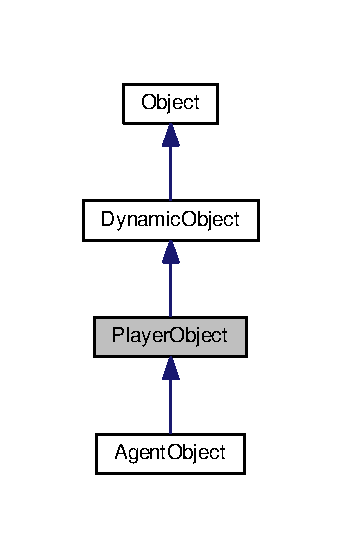
\includegraphics[width=164pt]{classPlayerObject__inherit__graph}
\end{center}
\end{figure}


Collaboration diagram for Player\+Object\+:
\nopagebreak
\begin{figure}[H]
\begin{center}
\leavevmode
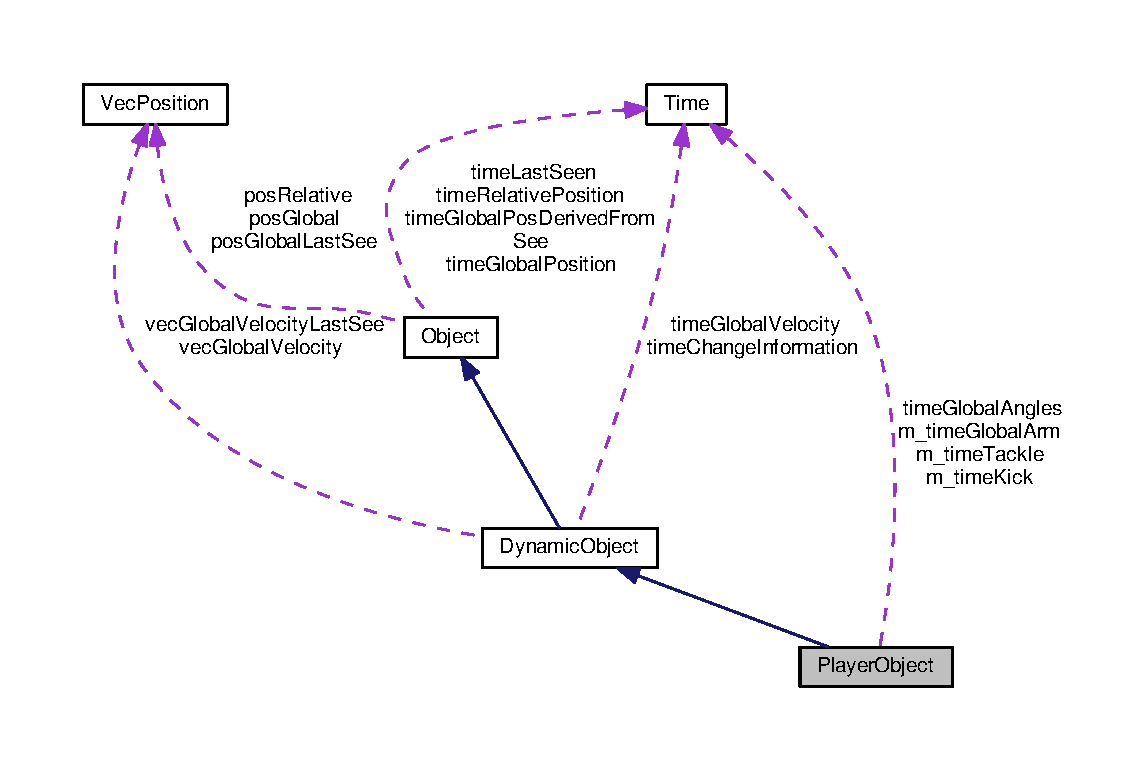
\includegraphics[width=350pt]{classPlayerObject__coll__graph}
\end{center}
\end{figure}
\subsection*{Public Member Functions}
\begin{DoxyCompactItemize}
\item 
\hyperlink{classPlayerObject_a0de74cb0566e6c5dc782b78d5f32501e}{Player\+Object} ()
\item 
void \hyperlink{classPlayerObject_a01d587f88139dddf2ca1b39a65523dd6}{show} (ostream \&os=cout)
\item 
void \hyperlink{classPlayerObject_a4234130be56d2e3ff23145e142c6c181}{show} (const char $\ast$str\+Team\+Name, ostream \&os=cout)
\item 
bool \hyperlink{classPlayerObject_a5947796f3dc132c3b407854be2036b8a}{set\+Possible\+Range} (\hyperlink{SoccerTypes_8h_ad4b701fa66e7d26c054ed15b7820c77c}{ObjectT} obj\+Min, \hyperlink{SoccerTypes_8h_ad4b701fa66e7d26c054ed15b7820c77c}{ObjectT} obj\+Max)
\item 
bool \hyperlink{classPlayerObject_a77e552342790af61652521545711f557}{is\+In\+Range} (\hyperlink{SoccerTypes_8h_ad4b701fa66e7d26c054ed15b7820c77c}{ObjectT} obj, bool b\+Team\+First)
\item 
\hyperlink{SoccerTypes_8h_ad4b701fa66e7d26c054ed15b7820c77c}{ObjectT} \hyperlink{classPlayerObject_abe5b800c89fb628ce146ec16e62c6311}{get\+Min\+Range} ()
\item 
\hyperlink{SoccerTypes_8h_ad4b701fa66e7d26c054ed15b7820c77c}{ObjectT} \hyperlink{classPlayerObject_a9eb9334ac8da63977cd2b43cd3a40631}{get\+Max\+Range} ()
\item 
bool \hyperlink{classPlayerObject_a90b5b23a4994d3d06d3302272f19aaac}{set\+Is\+Known\+Player} (bool b)
\item 
bool \hyperlink{classPlayerObject_a6565b68bec196218e4a151e6c8146b76}{get\+Is\+Known\+Player} () const 
\item 
bool \hyperlink{classPlayerObject_a6ae91cbdd7c298c2248701ac8977874f}{set\+Is\+Goalie} (bool b)
\item 
bool \hyperlink{classPlayerObject_a5aac2afb86495626e1c2dac2de9951a5}{get\+Is\+Goalie} () const 
\item 
bool \hyperlink{classPlayerObject_aefec5e6db9cde23f9db19c71b8c2e8f8}{set\+Relative\+Body\+Angle} (\hyperlink{Geometry_8h_a6bfe02ae9bb185092902092561ab2865}{Ang\+Deg} ang, \hyperlink{classTime}{Time} time)
\item 
\hyperlink{Geometry_8h_a6bfe02ae9bb185092902092561ab2865}{Ang\+Deg} \hyperlink{classPlayerObject_a951e253e5bfd263c7b8ad0b5f134e5a1}{get\+Relative\+Body\+Angle} () const 
\item 
bool \hyperlink{classPlayerObject_a3156d07e57edba4d4ce8645f0a91fdd3}{set\+Global\+Body\+Angle} (\hyperlink{Geometry_8h_a6bfe02ae9bb185092902092561ab2865}{Ang\+Deg} ang, \hyperlink{classTime}{Time} time)
\item 
\hyperlink{Geometry_8h_a6bfe02ae9bb185092902092561ab2865}{Ang\+Deg} \hyperlink{classPlayerObject_a8c32e163d9235c2ab0038ef738c74d22}{get\+Global\+Body\+Angle} () const 
\item 
bool \hyperlink{classPlayerObject_a09d956e2510f1572e66ec009c2172685}{set\+Relative\+Neck\+Angle} (\hyperlink{Geometry_8h_a6bfe02ae9bb185092902092561ab2865}{Ang\+Deg} ang, \hyperlink{classTime}{Time} time)
\item 
\hyperlink{Geometry_8h_a6bfe02ae9bb185092902092561ab2865}{Ang\+Deg} \hyperlink{classPlayerObject_a44cedbeb82f5a3db3f9f57855842b10d}{get\+Relative\+Neck\+Angle} () const 
\item 
bool \hyperlink{classPlayerObject_a1487d4de25978b04f1800f9483c1bb4a}{set\+Global\+Neck\+Angle} (\hyperlink{Geometry_8h_a6bfe02ae9bb185092902092561ab2865}{Ang\+Deg} ang, \hyperlink{classTime}{Time} time)
\item 
\hyperlink{Geometry_8h_a6bfe02ae9bb185092902092561ab2865}{Ang\+Deg} \hyperlink{classPlayerObject_ac7b84ff91ba81a2254313cbff5a1f180}{get\+Global\+Neck\+Angle} () const 
\item 
bool \hyperlink{classPlayerObject_a539526c5cd802b29cff3e6be04226e50}{set\+Time\+Relative\+Angles} (\hyperlink{classTime}{Time} time)
\item 
\hyperlink{classTime}{Time} \hyperlink{classPlayerObject_ac6c6455eb12ca19d41609df2a8e53a48}{get\+Time\+Relative\+Angles} () const 
\item 
bool \hyperlink{classPlayerObject_ad85554b74248deef8c12f5ab778faff0}{set\+Time\+Global\+Angles} (\hyperlink{classTime}{Time} time)
\item 
\hyperlink{classTime}{Time} \hyperlink{classPlayerObject_ac43f85956abb49ed3cc00f25fec1f791}{get\+Time\+Global\+Angles} () const 
\item 
bool \hyperlink{classPlayerObject_a4fc5e8e750666f488b8ecbb1bd40536f}{set\+Global\+Body\+Angle\+Last\+See} (\hyperlink{Geometry_8h_a6bfe02ae9bb185092902092561ab2865}{Ang\+Deg} ang)
\item 
\hyperlink{Geometry_8h_a6bfe02ae9bb185092902092561ab2865}{Ang\+Deg} \hyperlink{classPlayerObject_a724aad2574a807224bb5c353abe5a8bf}{get\+Global\+Body\+Angle\+Last\+See} () const 
\item 
bool \hyperlink{classPlayerObject_aa12cf1d604e46ccd61c8114924b870bd}{set\+Hetero\+Player\+Type} (int index)
\item 
int \hyperlink{classPlayerObject_a53fc8b930fcbc620d95fc5989bf288dc}{get\+Hetero\+Player\+Type} () const 
\item 
bool \hyperlink{classPlayerObject_ad8b1aeff152944b44cc805138dcb68de}{set\+Time\+Tackle} (\hyperlink{classTime}{Time} time)
\item 
\hyperlink{classTime}{Time} \hyperlink{classPlayerObject_a80e516083fc15dbf818c4f2c528ce97f}{get\+Time\+Tackle} () const 
\item 
bool \hyperlink{classPlayerObject_aa2254aec357b99da0d0cfd055609d477}{set\+Time\+Kick} (\hyperlink{classTime}{Time} time)
\item 
\hyperlink{classTime}{Time} \hyperlink{classPlayerObject_a2b1c6dd22798a9ba5d64d4d7071c0df3}{get\+Time\+Kick} () const 
\item 
bool \hyperlink{classPlayerObject_a78da26740a24cae0ed239d173b1fe010}{set\+Global\+Arm} (\hyperlink{Geometry_8h_a6bfe02ae9bb185092902092561ab2865}{Ang\+Deg} ang, \hyperlink{classTime}{Time} time)
\item 
\hyperlink{Geometry_8h_a6bfe02ae9bb185092902092561ab2865}{Ang\+Deg} \hyperlink{classPlayerObject_a2fdab6ebe5e659672a445940e6383d6c}{get\+Global\+Arm} () const 
\item 
bool \hyperlink{classPlayerObject_a5cc9b9c6dd889fb7bc74921d7165ebda}{set\+Time\+Global\+Arm} (\hyperlink{classTime}{Time} time)
\item 
\hyperlink{classTime}{Time} \hyperlink{classPlayerObject_abc3be47b0ce2c666237077812bf135b5}{get\+Time\+Global\+Arm} () const 
\end{DoxyCompactItemize}
\subsection*{Protected Attributes}
\begin{DoxyCompactItemize}
\item 
bool \hyperlink{classPlayerObject_a699d8554acd0197ba5393040bec150c4}{is\+Known\+Player}
\item 
\hyperlink{SoccerTypes_8h_ad4b701fa66e7d26c054ed15b7820c77c}{ObjectT} \hyperlink{classPlayerObject_a28e0c9103105adfd75b31192bd3f7027}{obj\+Range\+Min}
\item 
\hyperlink{SoccerTypes_8h_ad4b701fa66e7d26c054ed15b7820c77c}{ObjectT} \hyperlink{classPlayerObject_a2d42bf8573e4a7d6ade45b8395b84f50}{obj\+Range\+Max}
\item 
bool \hyperlink{classPlayerObject_a1e486f02cc1cd54d0c4dbf34b0146b06}{is\+Goalie}
\item 
\hyperlink{Geometry_8h_a6bfe02ae9bb185092902092561ab2865}{Ang\+Deg} \hyperlink{classPlayerObject_a1f6d18f264e9b817e9b96fbe88fe3782}{ang\+Global\+Body\+Angle}
\item 
\hyperlink{Geometry_8h_a6bfe02ae9bb185092902092561ab2865}{Ang\+Deg} \hyperlink{classPlayerObject_a98882a1394f93e2e72e3aeeb353129ab}{ang\+Global\+Neck\+Angle}
\item 
\hyperlink{Geometry_8h_a6bfe02ae9bb185092902092561ab2865}{Ang\+Deg} \hyperlink{classPlayerObject_a1d6d50f1bc562e21f3fb5ed93bfd389c}{ang\+Global\+Body\+Angle\+Last\+See}
\item 
\hyperlink{classTime}{Time} \hyperlink{classPlayerObject_aa734df386c6a0c55b28cd6530cbdb116}{time\+Global\+Angles}
\item 
int \hyperlink{classPlayerObject_a0a5a1732ec44a123c083ee7f71959354}{i\+Hetero\+Player\+Type}
\item 
\hyperlink{classTime}{Time} \hyperlink{classPlayerObject_aeb6b63098e15d4fb071a175c1240f83b}{m\+\_\+time\+Tackle}
\item 
\hyperlink{classTime}{Time} {\bfseries m\+\_\+time\+Kick}\hypertarget{classPlayerObject_a3e1ecfa81efdb3c8f1f47c92fb6f021c}{}\label{classPlayerObject_a3e1ecfa81efdb3c8f1f47c92fb6f021c}

\item 
\hyperlink{Geometry_8h_a6bfe02ae9bb185092902092561ab2865}{Ang\+Deg} \hyperlink{classPlayerObject_af93220d0f459af6f8fafa6c1a470fb09}{m\+\_\+ang\+Global\+Arm}
\item 
\hyperlink{classTime}{Time} \hyperlink{classPlayerObject_aefaa8321c6f8bb48527582212a5f2ac5}{m\+\_\+time\+Global\+Arm}
\end{DoxyCompactItemize}


\subsection{Detailed Description}
Class \hyperlink{classPlayerObject}{Player\+Object} contains Robo\+Cup information that is available for players. Different variables are added to the superclass \hyperlink{classDynamicObject}{Dynamic\+Object} 

\subsection{Constructor \& Destructor Documentation}
\index{Player\+Object@{Player\+Object}!Player\+Object@{Player\+Object}}
\index{Player\+Object@{Player\+Object}!Player\+Object@{Player\+Object}}
\subsubsection[{\texorpdfstring{Player\+Object()}{PlayerObject()}}]{\setlength{\rightskip}{0pt plus 5cm}Player\+Object\+::\+Player\+Object (
\begin{DoxyParamCaption}
{}
\end{DoxyParamCaption}
)}\hypertarget{classPlayerObject_a0de74cb0566e6c5dc782b78d5f32501e}{}\label{classPlayerObject_a0de74cb0566e6c5dc782b78d5f32501e}
This is the constructor for \hyperlink{classPlayerObject}{Player\+Object}. A \hyperlink{classPlayerObject}{Player\+Object} is created with all variables initialized to (illegal) default values 

\subsection{Member Function Documentation}
\index{Player\+Object@{Player\+Object}!get\+Global\+Arm@{get\+Global\+Arm}}
\index{get\+Global\+Arm@{get\+Global\+Arm}!Player\+Object@{Player\+Object}}
\subsubsection[{\texorpdfstring{get\+Global\+Arm() const }{getGlobalArm() const }}]{\setlength{\rightskip}{0pt plus 5cm}{\bf Ang\+Deg} Player\+Object\+::get\+Global\+Arm (
\begin{DoxyParamCaption}
{}
\end{DoxyParamCaption}
) const}\hypertarget{classPlayerObject_a2fdab6ebe5e659672a445940e6383d6c}{}\label{classPlayerObject_a2fdab6ebe5e659672a445940e6383d6c}
This method returns the global direction in which the arm of this object has last been observed to point. \index{Player\+Object@{Player\+Object}!get\+Global\+Body\+Angle@{get\+Global\+Body\+Angle}}
\index{get\+Global\+Body\+Angle@{get\+Global\+Body\+Angle}!Player\+Object@{Player\+Object}}
\subsubsection[{\texorpdfstring{get\+Global\+Body\+Angle() const }{getGlobalBodyAngle() const }}]{\setlength{\rightskip}{0pt plus 5cm}{\bf Ang\+Deg} Player\+Object\+::get\+Global\+Body\+Angle (
\begin{DoxyParamCaption}
{}
\end{DoxyParamCaption}
) const}\hypertarget{classPlayerObject_a8c32e163d9235c2ab0038ef738c74d22}{}\label{classPlayerObject_a8c32e163d9235c2ab0038ef738c74d22}
This method returns the global body angle of this object. This information is from the server time that is returned by \hyperlink{classPlayerObject_ac43f85956abb49ed3cc00f25fec1f791}{get\+Time\+Global\+Angles()}. \begin{DoxyReturn}{Returns}
global body angle of this object 
\end{DoxyReturn}
\index{Player\+Object@{Player\+Object}!get\+Global\+Body\+Angle\+Last\+See@{get\+Global\+Body\+Angle\+Last\+See}}
\index{get\+Global\+Body\+Angle\+Last\+See@{get\+Global\+Body\+Angle\+Last\+See}!Player\+Object@{Player\+Object}}
\subsubsection[{\texorpdfstring{get\+Global\+Body\+Angle\+Last\+See() const }{getGlobalBodyAngleLastSee() const }}]{\setlength{\rightskip}{0pt plus 5cm}{\bf Ang\+Deg} Player\+Object\+::get\+Global\+Body\+Angle\+Last\+See (
\begin{DoxyParamCaption}
{}
\end{DoxyParamCaption}
) const}\hypertarget{classPlayerObject_a724aad2574a807224bb5c353abe5a8bf}{}\label{classPlayerObject_a724aad2574a807224bb5c353abe5a8bf}
This method returns the global angle of the agent calculated after the last see message. The time of this information corresponds to \textquotesingle{}get\+Time\+Change\+Information\textquotesingle{}, since the change information arrives always together with the body and neck information.

\begin{DoxyReturn}{Returns}
global body angle derived from the last see message 
\end{DoxyReturn}
\index{Player\+Object@{Player\+Object}!get\+Global\+Neck\+Angle@{get\+Global\+Neck\+Angle}}
\index{get\+Global\+Neck\+Angle@{get\+Global\+Neck\+Angle}!Player\+Object@{Player\+Object}}
\subsubsection[{\texorpdfstring{get\+Global\+Neck\+Angle() const }{getGlobalNeckAngle() const }}]{\setlength{\rightskip}{0pt plus 5cm}{\bf Ang\+Deg} Player\+Object\+::get\+Global\+Neck\+Angle (
\begin{DoxyParamCaption}
{}
\end{DoxyParamCaption}
) const}\hypertarget{classPlayerObject_ac7b84ff91ba81a2254313cbff5a1f180}{}\label{classPlayerObject_ac7b84ff91ba81a2254313cbff5a1f180}
This method returns the global neck angle of this object. This information is from the time that is returned by \hyperlink{classPlayerObject_ac43f85956abb49ed3cc00f25fec1f791}{get\+Time\+Global\+Angles()}. \begin{DoxyReturn}{Returns}
global neck angle of this object 
\end{DoxyReturn}
\index{Player\+Object@{Player\+Object}!get\+Hetero\+Player\+Type@{get\+Hetero\+Player\+Type}}
\index{get\+Hetero\+Player\+Type@{get\+Hetero\+Player\+Type}!Player\+Object@{Player\+Object}}
\subsubsection[{\texorpdfstring{get\+Hetero\+Player\+Type() const }{getHeteroPlayerType() const }}]{\setlength{\rightskip}{0pt plus 5cm}int Player\+Object\+::get\+Hetero\+Player\+Type (
\begin{DoxyParamCaption}
{}
\end{DoxyParamCaption}
) const}\hypertarget{classPlayerObject_a53fc8b930fcbc620d95fc5989bf288dc}{}\label{classPlayerObject_a53fc8b930fcbc620d95fc5989bf288dc}
This method returns the heterogeneous index number of this player object. \begin{DoxyReturn}{Returns}
hetereogeneous index number 
\end{DoxyReturn}
\index{Player\+Object@{Player\+Object}!get\+Is\+Goalie@{get\+Is\+Goalie}}
\index{get\+Is\+Goalie@{get\+Is\+Goalie}!Player\+Object@{Player\+Object}}
\subsubsection[{\texorpdfstring{get\+Is\+Goalie() const }{getIsGoalie() const }}]{\setlength{\rightskip}{0pt plus 5cm}bool Player\+Object\+::get\+Is\+Goalie (
\begin{DoxyParamCaption}
{}
\end{DoxyParamCaption}
) const}\hypertarget{classPlayerObject_a5aac2afb86495626e1c2dac2de9951a5}{}\label{classPlayerObject_a5aac2afb86495626e1c2dac2de9951a5}
This method returns whether the current object is a goalie or not. \begin{DoxyReturn}{Returns}
bool indicating whether this dynamic object is a goalie or not 
\end{DoxyReturn}
\index{Player\+Object@{Player\+Object}!get\+Is\+Known\+Player@{get\+Is\+Known\+Player}}
\index{get\+Is\+Known\+Player@{get\+Is\+Known\+Player}!Player\+Object@{Player\+Object}}
\subsubsection[{\texorpdfstring{get\+Is\+Known\+Player() const }{getIsKnownPlayer() const }}]{\setlength{\rightskip}{0pt plus 5cm}bool Player\+Object\+::get\+Is\+Known\+Player (
\begin{DoxyParamCaption}
{}
\end{DoxyParamCaption}
) const}\hypertarget{classPlayerObject_a6565b68bec196218e4a151e6c8146b76}{}\label{classPlayerObject_a6565b68bec196218e4a151e6c8146b76}
This method returns whether the current object is a known player or not. A known player is a player of which we know the number. If we don\textquotesingle{}t know the player number of a player, the player is put at the index of a player that isn\textquotesingle{}t seen in a while and the is\+Known\+Player attribute is set to false. \begin{DoxyReturn}{Returns}
bool indicating whether player number is known 
\end{DoxyReturn}
\index{Player\+Object@{Player\+Object}!get\+Max\+Range@{get\+Max\+Range}}
\index{get\+Max\+Range@{get\+Max\+Range}!Player\+Object@{Player\+Object}}
\subsubsection[{\texorpdfstring{get\+Max\+Range()}{getMaxRange()}}]{\setlength{\rightskip}{0pt plus 5cm}{\bf ObjectT} Player\+Object\+::get\+Max\+Range (
\begin{DoxyParamCaption}
{}
\end{DoxyParamCaption}
)}\hypertarget{classPlayerObject_a9eb9334ac8da63977cd2b43cd3a40631}{}\label{classPlayerObject_a9eb9334ac8da63977cd2b43cd3a40631}
This method returns the maximal possible object type as set by \textquotesingle{}set\+Possible\+Range\textquotesingle{}. \begin{DoxyReturn}{Returns}
maximal possible object type 
\end{DoxyReturn}
\index{Player\+Object@{Player\+Object}!get\+Min\+Range@{get\+Min\+Range}}
\index{get\+Min\+Range@{get\+Min\+Range}!Player\+Object@{Player\+Object}}
\subsubsection[{\texorpdfstring{get\+Min\+Range()}{getMinRange()}}]{\setlength{\rightskip}{0pt plus 5cm}{\bf ObjectT} Player\+Object\+::get\+Min\+Range (
\begin{DoxyParamCaption}
{}
\end{DoxyParamCaption}
)}\hypertarget{classPlayerObject_abe5b800c89fb628ce146ec16e62c6311}{}\label{classPlayerObject_abe5b800c89fb628ce146ec16e62c6311}
This method returns the minimal possible object type as set by \textquotesingle{}set\+Possible\+Range\textquotesingle{}. \begin{DoxyReturn}{Returns}
minimal possible object type 
\end{DoxyReturn}
\index{Player\+Object@{Player\+Object}!get\+Relative\+Body\+Angle@{get\+Relative\+Body\+Angle}}
\index{get\+Relative\+Body\+Angle@{get\+Relative\+Body\+Angle}!Player\+Object@{Player\+Object}}
\subsubsection[{\texorpdfstring{get\+Relative\+Body\+Angle() const }{getRelativeBodyAngle() const }}]{\setlength{\rightskip}{0pt plus 5cm}{\bf Ang\+Deg} Player\+Object\+::get\+Relative\+Body\+Angle (
\begin{DoxyParamCaption}
{}
\end{DoxyParamCaption}
) const}\hypertarget{classPlayerObject_a951e253e5bfd263c7b8ad0b5f134e5a1}{}\label{classPlayerObject_a951e253e5bfd263c7b8ad0b5f134e5a1}
This method returns the relative body angle of this object. This information is from the server time that is returned by \hyperlink{classPlayerObject_ac6c6455eb12ca19d41609df2a8e53a48}{get\+Time\+Relative\+Angles()}.

\begin{DoxyReturn}{Returns}
relative body angle of this object 
\end{DoxyReturn}
\index{Player\+Object@{Player\+Object}!get\+Relative\+Neck\+Angle@{get\+Relative\+Neck\+Angle}}
\index{get\+Relative\+Neck\+Angle@{get\+Relative\+Neck\+Angle}!Player\+Object@{Player\+Object}}
\subsubsection[{\texorpdfstring{get\+Relative\+Neck\+Angle() const }{getRelativeNeckAngle() const }}]{\setlength{\rightskip}{0pt plus 5cm}{\bf Ang\+Deg} Player\+Object\+::get\+Relative\+Neck\+Angle (
\begin{DoxyParamCaption}
{}
\end{DoxyParamCaption}
) const}\hypertarget{classPlayerObject_a44cedbeb82f5a3db3f9f57855842b10d}{}\label{classPlayerObject_a44cedbeb82f5a3db3f9f57855842b10d}
This method returns the relative neck angle of this object. This information is from the time that is returned by \hyperlink{classPlayerObject_ac6c6455eb12ca19d41609df2a8e53a48}{get\+Time\+Relative\+Angles()}. \begin{DoxyReturn}{Returns}
relative neck angle of this object 
\end{DoxyReturn}
\index{Player\+Object@{Player\+Object}!get\+Time\+Global\+Angles@{get\+Time\+Global\+Angles}}
\index{get\+Time\+Global\+Angles@{get\+Time\+Global\+Angles}!Player\+Object@{Player\+Object}}
\subsubsection[{\texorpdfstring{get\+Time\+Global\+Angles() const }{getTimeGlobalAngles() const }}]{\setlength{\rightskip}{0pt plus 5cm}{\bf Time} Player\+Object\+::get\+Time\+Global\+Angles (
\begin{DoxyParamCaption}
{}
\end{DoxyParamCaption}
) const}\hypertarget{classPlayerObject_ac43f85956abb49ed3cc00f25fec1f791}{}\label{classPlayerObject_ac43f85956abb49ed3cc00f25fec1f791}
This method returns the server time in which the global body and neck angle of this object were calculated. \begin{DoxyReturn}{Returns}
time of the global neck and body information 
\end{DoxyReturn}
\index{Player\+Object@{Player\+Object}!get\+Time\+Global\+Arm@{get\+Time\+Global\+Arm}}
\index{get\+Time\+Global\+Arm@{get\+Time\+Global\+Arm}!Player\+Object@{Player\+Object}}
\subsubsection[{\texorpdfstring{get\+Time\+Global\+Arm() const }{getTimeGlobalArm() const }}]{\setlength{\rightskip}{0pt plus 5cm}{\bf Time} Player\+Object\+::get\+Time\+Global\+Arm (
\begin{DoxyParamCaption}
{}
\end{DoxyParamCaption}
) const}\hypertarget{classPlayerObject_abc3be47b0ce2c666237077812bf135b5}{}\label{classPlayerObject_abc3be47b0ce2c666237077812bf135b5}
This method returns the time that is related to the last time the arm of this object has been observed to point in the global direction returned by \textquotesingle{}get\+Global\+Arm\textquotesingle{}. \index{Player\+Object@{Player\+Object}!get\+Time\+Kick@{get\+Time\+Kick}}
\index{get\+Time\+Kick@{get\+Time\+Kick}!Player\+Object@{Player\+Object}}
\subsubsection[{\texorpdfstring{get\+Time\+Kick() const }{getTimeKick() const }}]{\setlength{\rightskip}{0pt plus 5cm}{\bf Time} Player\+Object\+::get\+Time\+Kick (
\begin{DoxyParamCaption}
{}
\end{DoxyParamCaption}
) const}\hypertarget{classPlayerObject_a2b1c6dd22798a9ba5d64d4d7071c0df3}{}\label{classPlayerObject_a2b1c6dd22798a9ba5d64d4d7071c0df3}
This method returns the cycle that is related to the last kick of this object. \index{Player\+Object@{Player\+Object}!get\+Time\+Relative\+Angles@{get\+Time\+Relative\+Angles}}
\index{get\+Time\+Relative\+Angles@{get\+Time\+Relative\+Angles}!Player\+Object@{Player\+Object}}
\subsubsection[{\texorpdfstring{get\+Time\+Relative\+Angles() const }{getTimeRelativeAngles() const }}]{\setlength{\rightskip}{0pt plus 5cm}{\bf Time} Player\+Object\+::get\+Time\+Relative\+Angles (
\begin{DoxyParamCaption}
{}
\end{DoxyParamCaption}
) const}\hypertarget{classPlayerObject_ac6c6455eb12ca19d41609df2a8e53a48}{}\label{classPlayerObject_ac6c6455eb12ca19d41609df2a8e53a48}
This method returns the server time in which the relative body and neck angle of this object were calculated. \begin{DoxyReturn}{Returns}
time of the relative neck and body information 
\end{DoxyReturn}
\index{Player\+Object@{Player\+Object}!get\+Time\+Tackle@{get\+Time\+Tackle}}
\index{get\+Time\+Tackle@{get\+Time\+Tackle}!Player\+Object@{Player\+Object}}
\subsubsection[{\texorpdfstring{get\+Time\+Tackle() const }{getTimeTackle() const }}]{\setlength{\rightskip}{0pt plus 5cm}{\bf Time} Player\+Object\+::get\+Time\+Tackle (
\begin{DoxyParamCaption}
{}
\end{DoxyParamCaption}
) const}\hypertarget{classPlayerObject_a80e516083fc15dbf818c4f2c528ce97f}{}\label{classPlayerObject_a80e516083fc15dbf818c4f2c528ce97f}
This method returns the time that is related to the last tackle of this object. \index{Player\+Object@{Player\+Object}!is\+In\+Range@{is\+In\+Range}}
\index{is\+In\+Range@{is\+In\+Range}!Player\+Object@{Player\+Object}}
\subsubsection[{\texorpdfstring{is\+In\+Range(\+Object\+T obj, bool b\+Team\+First)}{isInRange(ObjectT obj, bool bTeamFirst)}}]{\setlength{\rightskip}{0pt plus 5cm}bool Player\+Object\+::is\+In\+Range (
\begin{DoxyParamCaption}
\item[{{\bf ObjectT}}]{obj, }
\item[{bool}]{b\+Teammates\+First}
\end{DoxyParamCaption}
)}\hypertarget{classPlayerObject_a77e552342790af61652521545711f557}{}\label{classPlayerObject_a77e552342790af61652521545711f557}
This method returns a boolean indicating whether the supplied object type, is in the range of possible object types set by \textquotesingle{}set\+Possible\+Range\textquotesingle{}. 
\begin{DoxyParams}{Parameters}
{\em obj} & \hyperlink{classObject}{Object} type that should be checked \\
\hline
\end{DoxyParams}
\begin{DoxyReturn}{Returns}
boolean indicating whether \textquotesingle{}obj\textquotesingle{} is located in the range. 
\end{DoxyReturn}
\index{Player\+Object@{Player\+Object}!set\+Global\+Arm@{set\+Global\+Arm}}
\index{set\+Global\+Arm@{set\+Global\+Arm}!Player\+Object@{Player\+Object}}
\subsubsection[{\texorpdfstring{set\+Global\+Arm(\+Ang\+Deg ang, Time time)}{setGlobalArm(AngDeg ang, Time time)}}]{\setlength{\rightskip}{0pt plus 5cm}bool Player\+Object\+::set\+Global\+Arm (
\begin{DoxyParamCaption}
\item[{{\bf Ang\+Deg}}]{ang, }
\item[{{\bf Time}}]{time}
\end{DoxyParamCaption}
)}\hypertarget{classPlayerObject_a78da26740a24cae0ed239d173b1fe010}{}\label{classPlayerObject_a78da26740a24cae0ed239d173b1fe010}
This method sets the global direction in which the arm of this object has last been observed to point. The time related to this update is represented by time. \index{Player\+Object@{Player\+Object}!set\+Global\+Body\+Angle@{set\+Global\+Body\+Angle}}
\index{set\+Global\+Body\+Angle@{set\+Global\+Body\+Angle}!Player\+Object@{Player\+Object}}
\subsubsection[{\texorpdfstring{set\+Global\+Body\+Angle(\+Ang\+Deg ang, Time time)}{setGlobalBodyAngle(AngDeg ang, Time time)}}]{\setlength{\rightskip}{0pt plus 5cm}bool Player\+Object\+::set\+Global\+Body\+Angle (
\begin{DoxyParamCaption}
\item[{{\bf Ang\+Deg}}]{ang, }
\item[{{\bf Time}}]{time}
\end{DoxyParamCaption}
)}\hypertarget{classPlayerObject_a3156d07e57edba4d4ce8645f0a91fdd3}{}\label{classPlayerObject_a3156d07e57edba4d4ce8645f0a91fdd3}
This method sets the facing direction of the body and the time of this information (all global). 
\begin{DoxyParams}{Parameters}
{\em ang} & new global facing direction of body \\
\hline
{\em time} & time corresponding to the facing direction \\
\hline
\end{DoxyParams}
\begin{DoxyReturn}{Returns}
bool indicating whether the values were set 
\end{DoxyReturn}
\index{Player\+Object@{Player\+Object}!set\+Global\+Body\+Angle\+Last\+See@{set\+Global\+Body\+Angle\+Last\+See}}
\index{set\+Global\+Body\+Angle\+Last\+See@{set\+Global\+Body\+Angle\+Last\+See}!Player\+Object@{Player\+Object}}
\subsubsection[{\texorpdfstring{set\+Global\+Body\+Angle\+Last\+See(\+Ang\+Deg ang)}{setGlobalBodyAngleLastSee(AngDeg ang)}}]{\setlength{\rightskip}{0pt plus 5cm}bool Player\+Object\+::set\+Global\+Body\+Angle\+Last\+See (
\begin{DoxyParamCaption}
\item[{{\bf Ang\+Deg}}]{ang}
\end{DoxyParamCaption}
)}\hypertarget{classPlayerObject_a4fc5e8e750666f488b8ecbb1bd40536f}{}\label{classPlayerObject_a4fc5e8e750666f488b8ecbb1bd40536f}
This method sets the global angle of the agent calculated after the last see message. The time of this information corresponds to \textquotesingle{}get\+Time\+Change\+Information\textquotesingle{}, since the change information arrives always together with the body and neck information. \begin{DoxyReturn}{Returns}
global body angle derived from the last see message 
\end{DoxyReturn}
\index{Player\+Object@{Player\+Object}!set\+Global\+Neck\+Angle@{set\+Global\+Neck\+Angle}}
\index{set\+Global\+Neck\+Angle@{set\+Global\+Neck\+Angle}!Player\+Object@{Player\+Object}}
\subsubsection[{\texorpdfstring{set\+Global\+Neck\+Angle(\+Ang\+Deg ang, Time time)}{setGlobalNeckAngle(AngDeg ang, Time time)}}]{\setlength{\rightskip}{0pt plus 5cm}bool Player\+Object\+::set\+Global\+Neck\+Angle (
\begin{DoxyParamCaption}
\item[{{\bf Ang\+Deg}}]{ang, }
\item[{{\bf Time}}]{time}
\end{DoxyParamCaption}
)}\hypertarget{classPlayerObject_a1487d4de25978b04f1800f9483c1bb4a}{}\label{classPlayerObject_a1487d4de25978b04f1800f9483c1bb4a}
This method returns the facing direction of the neck and the time of this information (all global). 
\begin{DoxyParams}{Parameters}
{\em ang} & new global facing direction of neck \\
\hline
{\em i\+Time} & time facing direction was received \\
\hline
\end{DoxyParams}
\begin{DoxyReturn}{Returns}
bool indicating whether the values were set 
\end{DoxyReturn}
\index{Player\+Object@{Player\+Object}!set\+Hetero\+Player\+Type@{set\+Hetero\+Player\+Type}}
\index{set\+Hetero\+Player\+Type@{set\+Hetero\+Player\+Type}!Player\+Object@{Player\+Object}}
\subsubsection[{\texorpdfstring{set\+Hetero\+Player\+Type(int index)}{setHeteroPlayerType(int index)}}]{\setlength{\rightskip}{0pt plus 5cm}bool Player\+Object\+::set\+Hetero\+Player\+Type (
\begin{DoxyParamCaption}
\item[{int}]{index}
\end{DoxyParamCaption}
)}\hypertarget{classPlayerObject_aa12cf1d604e46ccd61c8114924b870bd}{}\label{classPlayerObject_aa12cf1d604e46ccd61c8114924b870bd}
This method sets the heterogeneous index number of this player object. 
\begin{DoxyParams}{Parameters}
{\em hetereogeneous} & index number \\
\hline
\end{DoxyParams}
\begin{DoxyReturn}{Returns}
bool indicating whether update was successful. 
\end{DoxyReturn}
\index{Player\+Object@{Player\+Object}!set\+Is\+Goalie@{set\+Is\+Goalie}}
\index{set\+Is\+Goalie@{set\+Is\+Goalie}!Player\+Object@{Player\+Object}}
\subsubsection[{\texorpdfstring{set\+Is\+Goalie(bool b)}{setIsGoalie(bool b)}}]{\setlength{\rightskip}{0pt plus 5cm}bool Player\+Object\+::set\+Is\+Goalie (
\begin{DoxyParamCaption}
\item[{bool}]{b}
\end{DoxyParamCaption}
)}\hypertarget{classPlayerObject_a6ae91cbdd7c298c2248701ac8977874f}{}\label{classPlayerObject_a6ae91cbdd7c298c2248701ac8977874f}
This method sets whether this dynamic object is a goalie or not. 
\begin{DoxyParams}{Parameters}
{\em b} & bool indicating whether this dynamic object is a goalie \\
\hline
\end{DoxyParams}
\begin{DoxyReturn}{Returns}
bool indicating whether value was set. 
\end{DoxyReturn}
\index{Player\+Object@{Player\+Object}!set\+Is\+Known\+Player@{set\+Is\+Known\+Player}}
\index{set\+Is\+Known\+Player@{set\+Is\+Known\+Player}!Player\+Object@{Player\+Object}}
\subsubsection[{\texorpdfstring{set\+Is\+Known\+Player(bool b)}{setIsKnownPlayer(bool b)}}]{\setlength{\rightskip}{0pt plus 5cm}bool Player\+Object\+::set\+Is\+Known\+Player (
\begin{DoxyParamCaption}
\item[{bool}]{b}
\end{DoxyParamCaption}
)}\hypertarget{classPlayerObject_a90b5b23a4994d3d06d3302272f19aaac}{}\label{classPlayerObject_a90b5b23a4994d3d06d3302272f19aaac}
This method sets whether this dynamic object is a known player or not. A known player is a player of which we know the number. If we don\textquotesingle{}t know the player number of a player, the player is put at the index of a player that isn\textquotesingle{}t seen in a while and the is\+Known\+Player attribute is set to false. 
\begin{DoxyParams}{Parameters}
{\em b} & bool indicating whether player number is known \\
\hline
\end{DoxyParams}
\begin{DoxyReturn}{Returns}
bool indicating whether value was set. 
\end{DoxyReturn}
\index{Player\+Object@{Player\+Object}!set\+Possible\+Range@{set\+Possible\+Range}}
\index{set\+Possible\+Range@{set\+Possible\+Range}!Player\+Object@{Player\+Object}}
\subsubsection[{\texorpdfstring{set\+Possible\+Range(\+Object\+T obj\+Min, Object\+T obj\+Max)}{setPossibleRange(ObjectT objMin, ObjectT objMax)}}]{\setlength{\rightskip}{0pt plus 5cm}bool Player\+Object\+::set\+Possible\+Range (
\begin{DoxyParamCaption}
\item[{{\bf ObjectT}}]{obj\+Min, }
\item[{{\bf ObjectT}}]{obj\+Max}
\end{DoxyParamCaption}
)}\hypertarget{classPlayerObject_a5947796f3dc132c3b407854be2036b8a}{}\label{classPlayerObject_a5947796f3dc132c3b407854be2036b8a}
This method sets the possible range from which this object must originate from. Since the ordening of objects in a \textquotesingle{}see\textquotesingle{} message is always the same (first teammates then opponents and always sorted by player number), it is possible to derive the range of objects from which the supplied information must originate. 
\begin{DoxyParams}{Parameters}
{\em obj\+Min} & minimum object type \\
\hline
{\em obj\+Max} & maximum object type \\
\hline
\end{DoxyParams}
\begin{DoxyReturn}{Returns}
bool indicating whether update was successful. 
\end{DoxyReturn}
\index{Player\+Object@{Player\+Object}!set\+Relative\+Body\+Angle@{set\+Relative\+Body\+Angle}}
\index{set\+Relative\+Body\+Angle@{set\+Relative\+Body\+Angle}!Player\+Object@{Player\+Object}}
\subsubsection[{\texorpdfstring{set\+Relative\+Body\+Angle(\+Ang\+Deg ang, Time time)}{setRelativeBodyAngle(AngDeg ang, Time time)}}]{\setlength{\rightskip}{0pt plus 5cm}bool Player\+Object\+::set\+Relative\+Body\+Angle (
\begin{DoxyParamCaption}
\item[{{\bf Ang\+Deg}}]{ang, }
\item[{{\bf Time}}]{time}
\end{DoxyParamCaption}
)}\hypertarget{classPlayerObject_aefec5e6db9cde23f9db19c71b8c2e8f8}{}\label{classPlayerObject_aefec5e6db9cde23f9db19c71b8c2e8f8}
This method sets the facing direction of the body and the time of this information (all relative to the agent). 
\begin{DoxyParams}{Parameters}
{\em ang} & new relative facing direction of body \\
\hline
{\em time} & time corresponding to the facing direction \\
\hline
\end{DoxyParams}
\begin{DoxyReturn}{Returns}
bool indicating whether the values were set 
\end{DoxyReturn}
\index{Player\+Object@{Player\+Object}!set\+Relative\+Neck\+Angle@{set\+Relative\+Neck\+Angle}}
\index{set\+Relative\+Neck\+Angle@{set\+Relative\+Neck\+Angle}!Player\+Object@{Player\+Object}}
\subsubsection[{\texorpdfstring{set\+Relative\+Neck\+Angle(\+Ang\+Deg ang, Time time)}{setRelativeNeckAngle(AngDeg ang, Time time)}}]{\setlength{\rightskip}{0pt plus 5cm}bool Player\+Object\+::set\+Relative\+Neck\+Angle (
\begin{DoxyParamCaption}
\item[{{\bf Ang\+Deg}}]{ang, }
\item[{{\bf Time}}]{time}
\end{DoxyParamCaption}
)}\hypertarget{classPlayerObject_a09d956e2510f1572e66ec009c2172685}{}\label{classPlayerObject_a09d956e2510f1572e66ec009c2172685}
This method returns the facing direction of the neck and the time of this information (all relative to the agent). 
\begin{DoxyParams}{Parameters}
{\em ang} & new relative facing direction of neck \\
\hline
{\em time} & time facing direction was received \\
\hline
\end{DoxyParams}
\begin{DoxyReturn}{Returns}
bool indicating whether the values were set 
\end{DoxyReturn}
\index{Player\+Object@{Player\+Object}!set\+Time\+Global\+Angles@{set\+Time\+Global\+Angles}}
\index{set\+Time\+Global\+Angles@{set\+Time\+Global\+Angles}!Player\+Object@{Player\+Object}}
\subsubsection[{\texorpdfstring{set\+Time\+Global\+Angles(\+Time time)}{setTimeGlobalAngles(Time time)}}]{\setlength{\rightskip}{0pt plus 5cm}bool Player\+Object\+::set\+Time\+Global\+Angles (
\begin{DoxyParamCaption}
\item[{{\bf Time}}]{time}
\end{DoxyParamCaption}
)}\hypertarget{classPlayerObject_ad85554b74248deef8c12f5ab778faff0}{}\label{classPlayerObject_ad85554b74248deef8c12f5ab778faff0}
This method sets the time the facing direction was calculated. 
\begin{DoxyParams}{Parameters}
{\em time} & time the facing direction was received \\
\hline
\end{DoxyParams}
\begin{DoxyReturn}{Returns}
bool indicating whether the values were set 
\end{DoxyReturn}
\index{Player\+Object@{Player\+Object}!set\+Time\+Global\+Arm@{set\+Time\+Global\+Arm}}
\index{set\+Time\+Global\+Arm@{set\+Time\+Global\+Arm}!Player\+Object@{Player\+Object}}
\subsubsection[{\texorpdfstring{set\+Time\+Global\+Arm(\+Time time)}{setTimeGlobalArm(Time time)}}]{\setlength{\rightskip}{0pt plus 5cm}bool Player\+Object\+::set\+Time\+Global\+Arm (
\begin{DoxyParamCaption}
\item[{{\bf Time}}]{time}
\end{DoxyParamCaption}
)}\hypertarget{classPlayerObject_a5cc9b9c6dd889fb7bc74921d7165ebda}{}\label{classPlayerObject_a5cc9b9c6dd889fb7bc74921d7165ebda}
This method sets the time that is related to the last time the arm of this object has been observed to point in the global direction returned by \textquotesingle{}get\+Global\+Arm\textquotesingle{}. \index{Player\+Object@{Player\+Object}!set\+Time\+Kick@{set\+Time\+Kick}}
\index{set\+Time\+Kick@{set\+Time\+Kick}!Player\+Object@{Player\+Object}}
\subsubsection[{\texorpdfstring{set\+Time\+Kick(\+Time time)}{setTimeKick(Time time)}}]{\setlength{\rightskip}{0pt plus 5cm}bool Player\+Object\+::set\+Time\+Kick (
\begin{DoxyParamCaption}
\item[{{\bf Time}}]{time}
\end{DoxyParamCaption}
)}\hypertarget{classPlayerObject_aa2254aec357b99da0d0cfd055609d477}{}\label{classPlayerObject_aa2254aec357b99da0d0cfd055609d477}
This method sets the cycle related to the last kick of this object. \index{Player\+Object@{Player\+Object}!set\+Time\+Relative\+Angles@{set\+Time\+Relative\+Angles}}
\index{set\+Time\+Relative\+Angles@{set\+Time\+Relative\+Angles}!Player\+Object@{Player\+Object}}
\subsubsection[{\texorpdfstring{set\+Time\+Relative\+Angles(\+Time time)}{setTimeRelativeAngles(Time time)}}]{\setlength{\rightskip}{0pt plus 5cm}bool Player\+Object\+::set\+Time\+Relative\+Angles (
\begin{DoxyParamCaption}
\item[{{\bf Time}}]{time}
\end{DoxyParamCaption}
)}\hypertarget{classPlayerObject_a539526c5cd802b29cff3e6be04226e50}{}\label{classPlayerObject_a539526c5cd802b29cff3e6be04226e50}
This method sets the time the facing direction was calculated. 
\begin{DoxyParams}{Parameters}
{\em time} & time the facing direction was received \\
\hline
\end{DoxyParams}
\begin{DoxyReturn}{Returns}
bool indicating whether the values were set 
\end{DoxyReturn}
\index{Player\+Object@{Player\+Object}!set\+Time\+Tackle@{set\+Time\+Tackle}}
\index{set\+Time\+Tackle@{set\+Time\+Tackle}!Player\+Object@{Player\+Object}}
\subsubsection[{\texorpdfstring{set\+Time\+Tackle(\+Time time)}{setTimeTackle(Time time)}}]{\setlength{\rightskip}{0pt plus 5cm}bool Player\+Object\+::set\+Time\+Tackle (
\begin{DoxyParamCaption}
\item[{{\bf Time}}]{time}
\end{DoxyParamCaption}
)}\hypertarget{classPlayerObject_ad8b1aeff152944b44cc805138dcb68de}{}\label{classPlayerObject_ad8b1aeff152944b44cc805138dcb68de}
This method sets the time related to the last tackle of this object. \index{Player\+Object@{Player\+Object}!show@{show}}
\index{show@{show}!Player\+Object@{Player\+Object}}
\subsubsection[{\texorpdfstring{show(ostream \&os=cout)}{show(ostream &os=cout)}}]{\setlength{\rightskip}{0pt plus 5cm}void Player\+Object\+::show (
\begin{DoxyParamCaption}
\item[{ostream \&}]{os = {\ttfamily cout}}
\end{DoxyParamCaption}
)\hspace{0.3cm}{\ttfamily [virtual]}}\hypertarget{classPlayerObject_a01d587f88139dddf2ca1b39a65523dd6}{}\label{classPlayerObject_a01d587f88139dddf2ca1b39a65523dd6}
This method prints the information about this \hyperlink{classPlayerObject}{Player\+Object} to the specified output stream. The variables are printed with the default team name. 
\begin{DoxyParams}{Parameters}
{\em os} & output stream to which output is written \\
\hline
\end{DoxyParams}


Implements \hyperlink{classObject_abdfad2372e7ec5f9aa271a1677653778}{Object}.



Reimplemented in \hyperlink{classAgentObject_a0043cea8d237828930412eb3c2b84e32}{Agent\+Object}.

\index{Player\+Object@{Player\+Object}!show@{show}}
\index{show@{show}!Player\+Object@{Player\+Object}}
\subsubsection[{\texorpdfstring{show(const char $\ast$str\+Team\+Name, ostream \&os=cout)}{show(const char *strTeamName, ostream &os=cout)}}]{\setlength{\rightskip}{0pt plus 5cm}void Player\+Object\+::show (
\begin{DoxyParamCaption}
\item[{const char $\ast$}]{str\+Team\+Name, }
\item[{ostream \&}]{os = {\ttfamily cout}}
\end{DoxyParamCaption}
)}\hypertarget{classPlayerObject_a4234130be56d2e3ff23145e142c6c181}{}\label{classPlayerObject_a4234130be56d2e3ff23145e142c6c181}
This method prints the information about this \hyperlink{classPlayerObject}{Player\+Object} to the specified output stream. The variables are printed with the specified team name. 
\begin{DoxyParams}{Parameters}
{\em str\+Team\+Name} & team name of this player object \\
\hline
{\em os} & output stream to which output is written \\
\hline
\end{DoxyParams}


\subsection{Member Data Documentation}
\index{Player\+Object@{Player\+Object}!ang\+Global\+Body\+Angle@{ang\+Global\+Body\+Angle}}
\index{ang\+Global\+Body\+Angle@{ang\+Global\+Body\+Angle}!Player\+Object@{Player\+Object}}
\subsubsection[{\texorpdfstring{ang\+Global\+Body\+Angle}{angGlobalBodyAngle}}]{\setlength{\rightskip}{0pt plus 5cm}{\bf Ang\+Deg} Player\+Object\+::ang\+Global\+Body\+Angle\hspace{0.3cm}{\ttfamily [protected]}}\hypertarget{classPlayerObject_a1f6d18f264e9b817e9b96fbe88fe3782}{}\label{classPlayerObject_a1f6d18f264e9b817e9b96fbe88fe3782}
Global body angle \index{Player\+Object@{Player\+Object}!ang\+Global\+Body\+Angle\+Last\+See@{ang\+Global\+Body\+Angle\+Last\+See}}
\index{ang\+Global\+Body\+Angle\+Last\+See@{ang\+Global\+Body\+Angle\+Last\+See}!Player\+Object@{Player\+Object}}
\subsubsection[{\texorpdfstring{ang\+Global\+Body\+Angle\+Last\+See}{angGlobalBodyAngleLastSee}}]{\setlength{\rightskip}{0pt plus 5cm}{\bf Ang\+Deg} Player\+Object\+::ang\+Global\+Body\+Angle\+Last\+See\hspace{0.3cm}{\ttfamily [protected]}}\hypertarget{classPlayerObject_a1d6d50f1bc562e21f3fb5ed93bfd389c}{}\label{classPlayerObject_a1d6d50f1bc562e21f3fb5ed93bfd389c}
Global body angle from last see msg \index{Player\+Object@{Player\+Object}!ang\+Global\+Neck\+Angle@{ang\+Global\+Neck\+Angle}}
\index{ang\+Global\+Neck\+Angle@{ang\+Global\+Neck\+Angle}!Player\+Object@{Player\+Object}}
\subsubsection[{\texorpdfstring{ang\+Global\+Neck\+Angle}{angGlobalNeckAngle}}]{\setlength{\rightskip}{0pt plus 5cm}{\bf Ang\+Deg} Player\+Object\+::ang\+Global\+Neck\+Angle\hspace{0.3cm}{\ttfamily [protected]}}\hypertarget{classPlayerObject_a98882a1394f93e2e72e3aeeb353129ab}{}\label{classPlayerObject_a98882a1394f93e2e72e3aeeb353129ab}
Global neck angle \index{Player\+Object@{Player\+Object}!i\+Hetero\+Player\+Type@{i\+Hetero\+Player\+Type}}
\index{i\+Hetero\+Player\+Type@{i\+Hetero\+Player\+Type}!Player\+Object@{Player\+Object}}
\subsubsection[{\texorpdfstring{i\+Hetero\+Player\+Type}{iHeteroPlayerType}}]{\setlength{\rightskip}{0pt plus 5cm}int Player\+Object\+::i\+Hetero\+Player\+Type\hspace{0.3cm}{\ttfamily [protected]}}\hypertarget{classPlayerObject_a0a5a1732ec44a123c083ee7f71959354}{}\label{classPlayerObject_a0a5a1732ec44a123c083ee7f71959354}
index of heterogeneous player type \index{Player\+Object@{Player\+Object}!is\+Goalie@{is\+Goalie}}
\index{is\+Goalie@{is\+Goalie}!Player\+Object@{Player\+Object}}
\subsubsection[{\texorpdfstring{is\+Goalie}{isGoalie}}]{\setlength{\rightskip}{0pt plus 5cm}bool Player\+Object\+::is\+Goalie\hspace{0.3cm}{\ttfamily [protected]}}\hypertarget{classPlayerObject_a1e486f02cc1cd54d0c4dbf34b0146b06}{}\label{classPlayerObject_a1e486f02cc1cd54d0c4dbf34b0146b06}
is this object a goalie \index{Player\+Object@{Player\+Object}!is\+Known\+Player@{is\+Known\+Player}}
\index{is\+Known\+Player@{is\+Known\+Player}!Player\+Object@{Player\+Object}}
\subsubsection[{\texorpdfstring{is\+Known\+Player}{isKnownPlayer}}]{\setlength{\rightskip}{0pt plus 5cm}bool Player\+Object\+::is\+Known\+Player\hspace{0.3cm}{\ttfamily [protected]}}\hypertarget{classPlayerObject_a699d8554acd0197ba5393040bec150c4}{}\label{classPlayerObject_a699d8554acd0197ba5393040bec150c4}
are we sure about player number \index{Player\+Object@{Player\+Object}!m\+\_\+ang\+Global\+Arm@{m\+\_\+ang\+Global\+Arm}}
\index{m\+\_\+ang\+Global\+Arm@{m\+\_\+ang\+Global\+Arm}!Player\+Object@{Player\+Object}}
\subsubsection[{\texorpdfstring{m\+\_\+ang\+Global\+Arm}{m_angGlobalArm}}]{\setlength{\rightskip}{0pt plus 5cm}{\bf Ang\+Deg} Player\+Object\+::m\+\_\+ang\+Global\+Arm\hspace{0.3cm}{\ttfamily [protected]}}\hypertarget{classPlayerObject_af93220d0f459af6f8fafa6c1a470fb09}{}\label{classPlayerObject_af93220d0f459af6f8fafa6c1a470fb09}
global pointing direction of arm \index{Player\+Object@{Player\+Object}!m\+\_\+time\+Global\+Arm@{m\+\_\+time\+Global\+Arm}}
\index{m\+\_\+time\+Global\+Arm@{m\+\_\+time\+Global\+Arm}!Player\+Object@{Player\+Object}}
\subsubsection[{\texorpdfstring{m\+\_\+time\+Global\+Arm}{m_timeGlobalArm}}]{\setlength{\rightskip}{0pt plus 5cm}{\bf Time} Player\+Object\+::m\+\_\+time\+Global\+Arm\hspace{0.3cm}{\ttfamily [protected]}}\hypertarget{classPlayerObject_aefaa8321c6f8bb48527582212a5f2ac5}{}\label{classPlayerObject_aefaa8321c6f8bb48527582212a5f2ac5}
time arm last seen \index{Player\+Object@{Player\+Object}!m\+\_\+time\+Tackle@{m\+\_\+time\+Tackle}}
\index{m\+\_\+time\+Tackle@{m\+\_\+time\+Tackle}!Player\+Object@{Player\+Object}}
\subsubsection[{\texorpdfstring{m\+\_\+time\+Tackle}{m_timeTackle}}]{\setlength{\rightskip}{0pt plus 5cm}{\bf Time} Player\+Object\+::m\+\_\+time\+Tackle\hspace{0.3cm}{\ttfamily [protected]}}\hypertarget{classPlayerObject_aeb6b63098e15d4fb071a175c1240f83b}{}\label{classPlayerObject_aeb6b63098e15d4fb071a175c1240f83b}
time tackle command was observerd \index{Player\+Object@{Player\+Object}!obj\+Range\+Max@{obj\+Range\+Max}}
\index{obj\+Range\+Max@{obj\+Range\+Max}!Player\+Object@{Player\+Object}}
\subsubsection[{\texorpdfstring{obj\+Range\+Max}{objRangeMax}}]{\setlength{\rightskip}{0pt plus 5cm}{\bf ObjectT} Player\+Object\+::obj\+Range\+Max\hspace{0.3cm}{\ttfamily [protected]}}\hypertarget{classPlayerObject_a2d42bf8573e4a7d6ade45b8395b84f50}{}\label{classPlayerObject_a2d42bf8573e4a7d6ade45b8395b84f50}
Maximum in range of possible player obj \index{Player\+Object@{Player\+Object}!obj\+Range\+Min@{obj\+Range\+Min}}
\index{obj\+Range\+Min@{obj\+Range\+Min}!Player\+Object@{Player\+Object}}
\subsubsection[{\texorpdfstring{obj\+Range\+Min}{objRangeMin}}]{\setlength{\rightskip}{0pt plus 5cm}{\bf ObjectT} Player\+Object\+::obj\+Range\+Min\hspace{0.3cm}{\ttfamily [protected]}}\hypertarget{classPlayerObject_a28e0c9103105adfd75b31192bd3f7027}{}\label{classPlayerObject_a28e0c9103105adfd75b31192bd3f7027}
Minimum in range of possible player obj \index{Player\+Object@{Player\+Object}!time\+Global\+Angles@{time\+Global\+Angles}}
\index{time\+Global\+Angles@{time\+Global\+Angles}!Player\+Object@{Player\+Object}}
\subsubsection[{\texorpdfstring{time\+Global\+Angles}{timeGlobalAngles}}]{\setlength{\rightskip}{0pt plus 5cm}{\bf Time} Player\+Object\+::time\+Global\+Angles\hspace{0.3cm}{\ttfamily [protected]}}\hypertarget{classPlayerObject_aa734df386c6a0c55b28cd6530cbdb116}{}\label{classPlayerObject_aa734df386c6a0c55b28cd6530cbdb116}
Server time of global angles 

The documentation for this class was generated from the following files\+:\begin{DoxyCompactItemize}
\item 
src/\hyperlink{Objects_8h}{Objects.\+h}\item 
src/\hyperlink{Objects_8cpp}{Objects.\+cpp}\end{DoxyCompactItemize}

\hypertarget{classPlayerSettings}{}\section{Player\+Settings Class Reference}
\label{classPlayerSettings}\index{Player\+Settings@{Player\+Settings}}


{\ttfamily \#include $<$Player\+Settings.\+h$>$}



Inheritance diagram for Player\+Settings\+:
\nopagebreak
\begin{figure}[H]
\begin{center}
\leavevmode
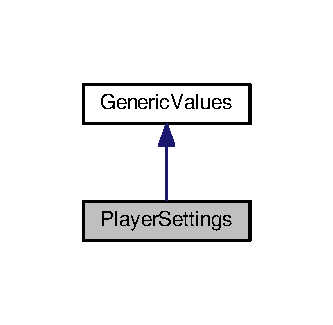
\includegraphics[width=160pt]{classPlayerSettings__inherit__graph}
\end{center}
\end{figure}


Collaboration diagram for Player\+Settings\+:
\nopagebreak
\begin{figure}[H]
\begin{center}
\leavevmode
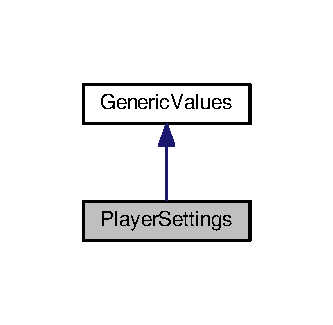
\includegraphics[width=160pt]{classPlayerSettings__coll__graph}
\end{center}
\end{figure}
\subsection*{Public Member Functions}
\begin{DoxyCompactItemize}
\item 
\hyperlink{classPlayerSettings_a0e73d43f99035a73efd94d51fd79e857}{Player\+Settings} ()
\item 
double \hyperlink{classPlayerSettings_a8113fecdb89ad86088d21e476405e4af}{get\+Player\+Conf\+Thr} () const 
\item 
bool \hyperlink{classPlayerSettings_a52b378a998340e01c41802fe4389f409}{set\+Player\+Conf\+Thr} (double d)
\item 
double \hyperlink{classPlayerSettings_a93667848519fcb52bd064d77e4a6e4f0}{get\+Player\+High\+Conf\+Thr} () const 
\item 
bool \hyperlink{classPlayerSettings_a833c0c4d30e2a625b2488ae488c5396c}{set\+Player\+High\+Conf\+Thr} (double d)
\item 
double \hyperlink{classPlayerSettings_ab8653b9920f4ad85ba19cc516523aa16}{get\+Ball\+Conf\+Thr} () const 
\item 
bool \hyperlink{classPlayerSettings_a738e71b55facd7256851dcbe7dfe24d4}{set\+Ball\+Conf\+Thr} (double d)
\item 
double \hyperlink{classPlayerSettings_a7b8fa5c91609d9993dc973cf6354c346}{get\+Player\+Dist\+Tolerance} () const 
\item 
bool \hyperlink{classPlayerSettings_adc174df162062e2274798376b017b741}{set\+Player\+Dist\+Tolerance} (double d)
\item 
double \hyperlink{classPlayerSettings_aaecbda8f2b284386d1349dbd32639d7f}{get\+Player\+When\+To\+Turn\+Angle} () const 
\item 
bool \hyperlink{classPlayerSettings_a224e566290a4c60c6523b1568c424583}{set\+Player\+When\+To\+Turn\+Angle} (double d)
\item 
double \hyperlink{classPlayerSettings_a42fcf95dc84b163c78d357170adba9bb}{get\+Player\+When\+To\+Kick} () const 
\item 
bool \hyperlink{classPlayerSettings_aefd09709861259de098e96e37e209aca}{set\+Player\+When\+To\+Kick} (double d)
\item 
int \hyperlink{classPlayerSettings_af7e1485098da6877a906fd202720cb3b}{get\+Player\+When\+To\+Intercept} () const 
\item 
bool \hyperlink{classPlayerSettings_ad18e3bf9f16696902e046a6547a8ac06}{set\+Player\+When\+To\+Intercept} (int i)
\item 
double \hyperlink{classPlayerSettings_a8aec92db959484bc9bb4364795fc08ff}{get\+Clear\+Ball\+Dist} () const 
\item 
bool \hyperlink{classPlayerSettings_a4f37c0ccbfed7bfa98f606d1b2bef022}{set\+Clear\+Ball\+Dist} (double d)
\item 
double \hyperlink{classPlayerSettings_af68da788df9cf34644d67f8aa55184e7}{get\+Clear\+Ball\+Opp\+Max\+Dist} () const 
\item 
bool \hyperlink{classPlayerSettings_a298a05574a863ec353b56cb47d2a67f9}{set\+Clear\+Ball\+Opp\+Max\+Dist} (double d)
\item 
double \hyperlink{classPlayerSettings_a909d44562ad9c2f1142ab0159e3a254f}{get\+Clear\+Ball\+To\+Side\+Angle} () const 
\item 
bool \hyperlink{classPlayerSettings_a102a026bd1761af8e86487fa478ceefc}{set\+Clear\+Ball\+To\+Side\+Angle} (double d)
\item 
double \hyperlink{classPlayerSettings_a2b7c5ff21f229e2c5a96f7206e9d201c}{get\+Cone\+Width} () const 
\item 
bool \hyperlink{classPlayerSettings_a2feb8cf242151163a39379036fbf8620}{set\+Cone\+Width} (double d)
\item 
double \hyperlink{classPlayerSettings_aa235850caad09cfc9b24df0875ebddf0}{get\+Pass\+End\+Speed} () const 
\item 
bool \hyperlink{classPlayerSettings_a88c8d11e365bedd3c0e41f9481f01b41}{set\+Pass\+End\+Speed} (double d)
\item 
double \hyperlink{classPlayerSettings_a40a3ebc661928cd2c96079b2df08b567}{get\+Fast\+Pass\+End\+Speed} () const 
\item 
bool \hyperlink{classPlayerSettings_aef63440c0e432d3c0dd2b9db67453682}{set\+Fast\+Pass\+End\+Speed} (double d)
\item 
double \hyperlink{classPlayerSettings_aa6b33b183254ce9676e53576d6c5612d}{get\+Pass\+ExtraX} () const 
\item 
bool \hyperlink{classPlayerSettings_a96d73a1142897fe589e8061e0ffb530b}{set\+Pass\+ExtraX} (double d)
\item 
double \hyperlink{classPlayerSettings_a104ab0696a9c7c0724af5b7780b1eeec}{get\+Fraction\+Wait\+No\+See} () const 
\item 
bool \hyperlink{classPlayerSettings_a764092fb3ea08f78fbc752fd61077205}{set\+Fraction\+Wait\+No\+See} (double d)
\item 
double \hyperlink{classPlayerSettings_a070019f8a54cd8817040c16431102285}{get\+Fraction\+Wait\+See\+Begin} () const 
\item 
bool \hyperlink{classPlayerSettings_abe5b1dba17f778d04a4df0e4b40eca00}{set\+Fraction\+Wait\+See\+Begin} (double d)
\item 
double \hyperlink{classPlayerSettings_a9c1193663c2f561c9f0202aa4d196545}{get\+Fraction\+Wait\+See\+End} () const 
\item 
bool \hyperlink{classPlayerSettings_a66755a30f30ec5c5b3805f00bd7a19af}{set\+Fraction\+Wait\+See\+End} (double d)
\item 
double \hyperlink{classPlayerSettings_a086a436c94b3bc028be7a086e54c8a3b}{get\+Mark\+Distance} () const 
\item 
bool \hyperlink{classPlayerSettings_aff59deb623936e9097ae02943b741c6a}{set\+Mark\+Distance} (double d)
\item 
double \hyperlink{classPlayerSettings_a4affb48ac93b91c53d1f34192af794bc}{get\+Strat\+Area\+Radius} () const 
\item 
bool \hyperlink{classPlayerSettings_a62ffc24e3bee58be063d18c625de1812}{set\+Strat\+Area\+Radius} (double d)
\item 
double \hyperlink{classPlayerSettings_aa6edaba41c21f4c6d61cf604f4f8168d}{get\+Shoot\+Risk\+Probability} () const 
\item 
bool \hyperlink{classPlayerSettings_afa6277adc38471faed9564c94418f6ce}{set\+Shoot\+Risk\+Probability} (double d)
\item 
int \hyperlink{classPlayerSettings_a3b730f8eca3e6cf26bfac8f31e1d28ad}{get\+Cycles\+Catch\+Wait} () const 
\item 
bool \hyperlink{classPlayerSettings_a0c2a72088a0280f2e83dee660ec063ed}{set\+Cycles\+Catch\+Wait} (int i)
\item 
int \hyperlink{classPlayerSettings_af829a56f3cde24de4212c404741eccda}{get\+Server\+Time\+Out} () const 
\item 
bool \hyperlink{classPlayerSettings_af1c207e73ba987772f742185ff3fa022}{set\+Server\+Time\+Out} (int i)
\item 
double \hyperlink{classPlayerSettings_a007673defd340921ec31f7b7f54cf65e}{get\+Dribble\+Ang\+Thr} () const 
\item 
bool \hyperlink{classPlayerSettings_a5cae40fcedeec1de188471fdd9a3d725}{set\+Dribble\+Ang\+Thr} (double d)
\item 
double \hyperlink{classPlayerSettings_ac9d8835351e0151acee1929f7391b2f9}{get\+Turn\+With\+Ball\+Ang\+Thr} () const 
\item 
bool \hyperlink{classPlayerSettings_a1a8ee5dedb30f14407a755177652580e}{set\+Turn\+With\+Ball\+Ang\+Thr} (double d)
\item 
double \hyperlink{classPlayerSettings_a2fa85d0f73fdef734ab6fbd46f12b121}{get\+Turn\+With\+Ball\+Freeze\+Thr} () const 
\item 
bool \hyperlink{classPlayerSettings_aa817e0fc8b28cf0dee69f361832c4424}{set\+Turn\+With\+Ball\+Freeze\+Thr} (double d)
\item 
int \hyperlink{classPlayerSettings_ad95999dfaa22c3f87172dd36681d3ea7}{get\+Initial\+Formation} () const 
\item 
bool \hyperlink{classPlayerSettings_ad36b059197447a7af145681c766a8025}{set\+Initial\+Formation} (int i)
\item 
double \hyperlink{classPlayerSettings_adb13109c4ecb09cd3a2f857e04df0f27}{get\+Max\+Y\+Percentage} () const 
\item 
bool \hyperlink{classPlayerSettings_a240dd1caecdd7f225a364e288ea70275}{set\+Max\+Y\+Percentage} (double d)
\end{DoxyCompactItemize}


\subsection{Detailed Description}
This class contains all the settings that are important for the client (agent) to determine its actions. It contains mostly threshold values to determine whether a certain kind of actions should be taken or not. Furthermore this class contains all the standard set-\/ and get methods for manipulating these values. Although it is normally not the case that these values are changed at runtime. The \hyperlink{classPlayerSettings}{Player\+Settings} class is a subclass of the \hyperlink{classGenericValues}{Generic\+Values} class and therefore each value in this class can be reached through the string name of the corresponding parameter. This may be helpful when the parameters are taken from a configuration file. 

\subsection{Constructor \& Destructor Documentation}
\index{Player\+Settings@{Player\+Settings}!Player\+Settings@{Player\+Settings}}
\index{Player\+Settings@{Player\+Settings}!Player\+Settings@{Player\+Settings}}
\subsubsection[{\texorpdfstring{Player\+Settings()}{PlayerSettings()}}]{\setlength{\rightskip}{0pt plus 5cm}Player\+Settings\+::\+Player\+Settings (
\begin{DoxyParamCaption}
{}
\end{DoxyParamCaption}
)}\hypertarget{classPlayerSettings_a0e73d43f99035a73efd94d51fd79e857}{}\label{classPlayerSettings_a0e73d43f99035a73efd94d51fd79e857}
This method initializes all client settings and adds these to the generic values class with the effect that they can referenced by their textual name. 

\subsection{Member Function Documentation}
\index{Player\+Settings@{Player\+Settings}!get\+Ball\+Conf\+Thr@{get\+Ball\+Conf\+Thr}}
\index{get\+Ball\+Conf\+Thr@{get\+Ball\+Conf\+Thr}!Player\+Settings@{Player\+Settings}}
\subsubsection[{\texorpdfstring{get\+Ball\+Conf\+Thr() const }{getBallConfThr() const }}]{\setlength{\rightskip}{0pt plus 5cm}double Player\+Settings\+::get\+Ball\+Conf\+Thr (
\begin{DoxyParamCaption}
{}
\end{DoxyParamCaption}
) const}\hypertarget{classPlayerSettings_ab8653b9920f4ad85ba19cc516523aa16}{}\label{classPlayerSettings_ab8653b9920f4ad85ba19cc516523aa16}
This method returns the confidence threshold below which ball information is assumed illegal. \begin{DoxyReturn}{Returns}
ball confidence threshold 
\end{DoxyReturn}
\index{Player\+Settings@{Player\+Settings}!get\+Clear\+Ball\+Dist@{get\+Clear\+Ball\+Dist}}
\index{get\+Clear\+Ball\+Dist@{get\+Clear\+Ball\+Dist}!Player\+Settings@{Player\+Settings}}
\subsubsection[{\texorpdfstring{get\+Clear\+Ball\+Dist() const }{getClearBallDist() const }}]{\setlength{\rightskip}{0pt plus 5cm}double Player\+Settings\+::get\+Clear\+Ball\+Dist (
\begin{DoxyParamCaption}
{}
\end{DoxyParamCaption}
) const}\hypertarget{classPlayerSettings_a8aec92db959484bc9bb4364795fc08ff}{}\label{classPlayerSettings_a8aec92db959484bc9bb4364795fc08ff}
This method returns the clear ball distance. When a clear ball is performed, the ball is aimed to a point just in front of the penalty area of the opponent. This method returns the distance before the penalty area to which the ball is aimed. \begin{DoxyReturn}{Returns}
clear ball distance before opponent penalty area 
\end{DoxyReturn}
\index{Player\+Settings@{Player\+Settings}!get\+Clear\+Ball\+Opp\+Max\+Dist@{get\+Clear\+Ball\+Opp\+Max\+Dist}}
\index{get\+Clear\+Ball\+Opp\+Max\+Dist@{get\+Clear\+Ball\+Opp\+Max\+Dist}!Player\+Settings@{Player\+Settings}}
\subsubsection[{\texorpdfstring{get\+Clear\+Ball\+Opp\+Max\+Dist() const }{getClearBallOppMaxDist() const }}]{\setlength{\rightskip}{0pt plus 5cm}double Player\+Settings\+::get\+Clear\+Ball\+Opp\+Max\+Dist (
\begin{DoxyParamCaption}
{}
\end{DoxyParamCaption}
) const}\hypertarget{classPlayerSettings_af68da788df9cf34644d67f8aa55184e7}{}\label{classPlayerSettings_af68da788df9cf34644d67f8aa55184e7}
This method returns the distance in which opponents are taken into account when a clear ball is issued. \begin{DoxyReturn}{Returns}
maximum opponent distance for clear ball. 
\end{DoxyReturn}
\index{Player\+Settings@{Player\+Settings}!get\+Clear\+Ball\+To\+Side\+Angle@{get\+Clear\+Ball\+To\+Side\+Angle}}
\index{get\+Clear\+Ball\+To\+Side\+Angle@{get\+Clear\+Ball\+To\+Side\+Angle}!Player\+Settings@{Player\+Settings}}
\subsubsection[{\texorpdfstring{get\+Clear\+Ball\+To\+Side\+Angle() const }{getClearBallToSideAngle() const }}]{\setlength{\rightskip}{0pt plus 5cm}double Player\+Settings\+::get\+Clear\+Ball\+To\+Side\+Angle (
\begin{DoxyParamCaption}
{}
\end{DoxyParamCaption}
) const}\hypertarget{classPlayerSettings_a909d44562ad9c2f1142ab0159e3a254f}{}\label{classPlayerSettings_a909d44562ad9c2f1142ab0159e3a254f}
This method returns the minimum needed angle for a clear ball to the side. \begin{DoxyReturn}{Returns}
minimum needed angle for clear ball to side 
\end{DoxyReturn}
\index{Player\+Settings@{Player\+Settings}!get\+Cone\+Width@{get\+Cone\+Width}}
\index{get\+Cone\+Width@{get\+Cone\+Width}!Player\+Settings@{Player\+Settings}}
\subsubsection[{\texorpdfstring{get\+Cone\+Width() const }{getConeWidth() const }}]{\setlength{\rightskip}{0pt plus 5cm}double Player\+Settings\+::get\+Cone\+Width (
\begin{DoxyParamCaption}
{}
\end{DoxyParamCaption}
) const}\hypertarget{classPlayerSettings_a2b7c5ff21f229e2c5a96f7206e9d201c}{}\label{classPlayerSettings_a2b7c5ff21f229e2c5a96f7206e9d201c}
This method returns the cone width that is used to check for opponents when passing to a player. A pass is only performed when no opponents are in the cone. The cone is specified as the width to one side after distance 1. So for a value of 0.\+5 the cone angle equals 45 (22.\+5 to both sides). \begin{DoxyReturn}{Returns}
cone width in which no opponents are allowed when passing 
\end{DoxyReturn}
\index{Player\+Settings@{Player\+Settings}!get\+Cycles\+Catch\+Wait@{get\+Cycles\+Catch\+Wait}}
\index{get\+Cycles\+Catch\+Wait@{get\+Cycles\+Catch\+Wait}!Player\+Settings@{Player\+Settings}}
\subsubsection[{\texorpdfstring{get\+Cycles\+Catch\+Wait() const }{getCyclesCatchWait() const }}]{\setlength{\rightskip}{0pt plus 5cm}int Player\+Settings\+::get\+Cycles\+Catch\+Wait (
\begin{DoxyParamCaption}
{}
\end{DoxyParamCaption}
) const}\hypertarget{classPlayerSettings_a3b730f8eca3e6cf26bfac8f31e1d28ad}{}\label{classPlayerSettings_a3b730f8eca3e6cf26bfac8f31e1d28ad}
This method returns the number of cycles waited by the goalkeeper after he has catched the ball. \begin{DoxyReturn}{Returns}
number of cycles goalkeeper waits after catch 
\end{DoxyReturn}
\index{Player\+Settings@{Player\+Settings}!get\+Dribble\+Ang\+Thr@{get\+Dribble\+Ang\+Thr}}
\index{get\+Dribble\+Ang\+Thr@{get\+Dribble\+Ang\+Thr}!Player\+Settings@{Player\+Settings}}
\subsubsection[{\texorpdfstring{get\+Dribble\+Ang\+Thr() const }{getDribbleAngThr() const }}]{\setlength{\rightskip}{0pt plus 5cm}double Player\+Settings\+::get\+Dribble\+Ang\+Thr (
\begin{DoxyParamCaption}
{}
\end{DoxyParamCaption}
) const}\hypertarget{classPlayerSettings_a007673defd340921ec31f7b7f54cf65e}{}\label{classPlayerSettings_a007673defd340921ec31f7b7f54cf65e}
This method returns the threshold to determine when the agent turns towards the dribble direction when dribbling. When the global angle difference is larger than this value, the agent performs a turn\+With\+Ball\+To. \begin{DoxyReturn}{Returns}
threshold value for angle 
\end{DoxyReturn}
\index{Player\+Settings@{Player\+Settings}!get\+Fast\+Pass\+End\+Speed@{get\+Fast\+Pass\+End\+Speed}}
\index{get\+Fast\+Pass\+End\+Speed@{get\+Fast\+Pass\+End\+Speed}!Player\+Settings@{Player\+Settings}}
\subsubsection[{\texorpdfstring{get\+Fast\+Pass\+End\+Speed() const }{getFastPassEndSpeed() const }}]{\setlength{\rightskip}{0pt plus 5cm}double Player\+Settings\+::get\+Fast\+Pass\+End\+Speed (
\begin{DoxyParamCaption}
{}
\end{DoxyParamCaption}
) const}\hypertarget{classPlayerSettings_a40a3ebc661928cd2c96079b2df08b567}{}\label{classPlayerSettings_a40a3ebc661928cd2c96079b2df08b567}
This method returns the desired end speed for the ball when a fast pass is performed. \begin{DoxyReturn}{Returns}
desired end speed for ball when it is passed fast 
\end{DoxyReturn}
\index{Player\+Settings@{Player\+Settings}!get\+Fraction\+Wait\+No\+See@{get\+Fraction\+Wait\+No\+See}}
\index{get\+Fraction\+Wait\+No\+See@{get\+Fraction\+Wait\+No\+See}!Player\+Settings@{Player\+Settings}}
\subsubsection[{\texorpdfstring{get\+Fraction\+Wait\+No\+See() const }{getFractionWaitNoSee() const }}]{\setlength{\rightskip}{0pt plus 5cm}double Player\+Settings\+::get\+Fraction\+Wait\+No\+See (
\begin{DoxyParamCaption}
{}
\end{DoxyParamCaption}
) const}\hypertarget{classPlayerSettings_a104ab0696a9c7c0724af5b7780b1eeec}{}\label{classPlayerSettings_a104ab0696a9c7c0724af5b7780b1eeec}
This method returns the fraction of the simulation step that is waited before an action is sent to the server in case no see message will arrive in this cycle. \begin{DoxyReturn}{Returns}
fraction of simulation step that is waited when no see arrives 
\end{DoxyReturn}
\index{Player\+Settings@{Player\+Settings}!get\+Fraction\+Wait\+See\+Begin@{get\+Fraction\+Wait\+See\+Begin}}
\index{get\+Fraction\+Wait\+See\+Begin@{get\+Fraction\+Wait\+See\+Begin}!Player\+Settings@{Player\+Settings}}
\subsubsection[{\texorpdfstring{get\+Fraction\+Wait\+See\+Begin() const }{getFractionWaitSeeBegin() const }}]{\setlength{\rightskip}{0pt plus 5cm}double Player\+Settings\+::get\+Fraction\+Wait\+See\+Begin (
\begin{DoxyParamCaption}
{}
\end{DoxyParamCaption}
) const}\hypertarget{classPlayerSettings_a070019f8a54cd8817040c16431102285}{}\label{classPlayerSettings_a070019f8a54cd8817040c16431102285}
This method returns the fraction of the simulation step that is waited before an action is sent to the server in case the see message will arrive in the first half of the cycle. \begin{DoxyReturn}{Returns}
fraction of simulation step that is waited when see arrives in first half of the cycle 
\end{DoxyReturn}
\index{Player\+Settings@{Player\+Settings}!get\+Fraction\+Wait\+See\+End@{get\+Fraction\+Wait\+See\+End}}
\index{get\+Fraction\+Wait\+See\+End@{get\+Fraction\+Wait\+See\+End}!Player\+Settings@{Player\+Settings}}
\subsubsection[{\texorpdfstring{get\+Fraction\+Wait\+See\+End() const }{getFractionWaitSeeEnd() const }}]{\setlength{\rightskip}{0pt plus 5cm}double Player\+Settings\+::get\+Fraction\+Wait\+See\+End (
\begin{DoxyParamCaption}
{}
\end{DoxyParamCaption}
) const}\hypertarget{classPlayerSettings_a9c1193663c2f561c9f0202aa4d196545}{}\label{classPlayerSettings_a9c1193663c2f561c9f0202aa4d196545}
This method returns the fraction of the simulation step that is waited before an action is sent to the server in case the see message will arrive in the second half of the cycle. \begin{DoxyReturn}{Returns}
fraction of simulation step that is waited when see arrives in second half of the cycle 
\end{DoxyReturn}
\index{Player\+Settings@{Player\+Settings}!get\+Initial\+Formation@{get\+Initial\+Formation}}
\index{get\+Initial\+Formation@{get\+Initial\+Formation}!Player\+Settings@{Player\+Settings}}
\subsubsection[{\texorpdfstring{get\+Initial\+Formation() const }{getInitialFormation() const }}]{\setlength{\rightskip}{0pt plus 5cm}int Player\+Settings\+::get\+Initial\+Formation (
\begin{DoxyParamCaption}
{}
\end{DoxyParamCaption}
) const}\hypertarget{classPlayerSettings_ad95999dfaa22c3f87172dd36681d3ea7}{}\label{classPlayerSettings_ad95999dfaa22c3f87172dd36681d3ea7}
This method returns the initial formation of the team. \begin{DoxyReturn}{Returns}
number of cycles goalkeeper waits after catch 
\end{DoxyReturn}
\index{Player\+Settings@{Player\+Settings}!get\+Mark\+Distance@{get\+Mark\+Distance}}
\index{get\+Mark\+Distance@{get\+Mark\+Distance}!Player\+Settings@{Player\+Settings}}
\subsubsection[{\texorpdfstring{get\+Mark\+Distance() const }{getMarkDistance() const }}]{\setlength{\rightskip}{0pt plus 5cm}double Player\+Settings\+::get\+Mark\+Distance (
\begin{DoxyParamCaption}
{}
\end{DoxyParamCaption}
) const}\hypertarget{classPlayerSettings_a086a436c94b3bc028be7a086e54c8a3b}{}\label{classPlayerSettings_a086a436c94b3bc028be7a086e54c8a3b}
This method returns the desired distance to an opponent which should be marked. \begin{DoxyReturn}{Returns}
desired marking distance to an opponent 
\end{DoxyReturn}
\index{Player\+Settings@{Player\+Settings}!get\+Max\+Y\+Percentage@{get\+Max\+Y\+Percentage}}
\index{get\+Max\+Y\+Percentage@{get\+Max\+Y\+Percentage}!Player\+Settings@{Player\+Settings}}
\subsubsection[{\texorpdfstring{get\+Max\+Y\+Percentage() const }{getMaxYPercentage() const }}]{\setlength{\rightskip}{0pt plus 5cm}double Player\+Settings\+::get\+Max\+Y\+Percentage (
\begin{DoxyParamCaption}
{}
\end{DoxyParamCaption}
) const}\hypertarget{classPlayerSettings_adb13109c4ecb09cd3a2f857e04df0f27}{}\label{classPlayerSettings_adb13109c4ecb09cd3a2f857e04df0f27}
This method returns the percentage of the field width. The corresponding y position is the maximum allowed y position for a player\textquotesingle{}s strategic position. \begin{DoxyReturn}{Returns}
maximum y percentage on the field. 
\end{DoxyReturn}
\index{Player\+Settings@{Player\+Settings}!get\+Pass\+End\+Speed@{get\+Pass\+End\+Speed}}
\index{get\+Pass\+End\+Speed@{get\+Pass\+End\+Speed}!Player\+Settings@{Player\+Settings}}
\subsubsection[{\texorpdfstring{get\+Pass\+End\+Speed() const }{getPassEndSpeed() const }}]{\setlength{\rightskip}{0pt plus 5cm}double Player\+Settings\+::get\+Pass\+End\+Speed (
\begin{DoxyParamCaption}
{}
\end{DoxyParamCaption}
) const}\hypertarget{classPlayerSettings_aa235850caad09cfc9b24df0875ebddf0}{}\label{classPlayerSettings_aa235850caad09cfc9b24df0875ebddf0}
This method returns the desired end speed for the ball when a normal pass is performed. \begin{DoxyReturn}{Returns}
desired end speed for ball 
\end{DoxyReturn}
\index{Player\+Settings@{Player\+Settings}!get\+Pass\+ExtraX@{get\+Pass\+ExtraX}}
\index{get\+Pass\+ExtraX@{get\+Pass\+ExtraX}!Player\+Settings@{Player\+Settings}}
\subsubsection[{\texorpdfstring{get\+Pass\+Extra\+X() const }{getPassExtraX() const }}]{\setlength{\rightskip}{0pt plus 5cm}double Player\+Settings\+::get\+Pass\+ExtraX (
\begin{DoxyParamCaption}
{}
\end{DoxyParamCaption}
) const}\hypertarget{classPlayerSettings_aa6b33b183254ce9676e53576d6c5612d}{}\label{classPlayerSettings_aa6b33b183254ce9676e53576d6c5612d}
This method returns the x value that can be added to the position of a teammate when a leading pass to this teammate is performed. \begin{DoxyReturn}{Returns}
x value added to teammate to which is passed 
\end{DoxyReturn}
\index{Player\+Settings@{Player\+Settings}!get\+Player\+Conf\+Thr@{get\+Player\+Conf\+Thr}}
\index{get\+Player\+Conf\+Thr@{get\+Player\+Conf\+Thr}!Player\+Settings@{Player\+Settings}}
\subsubsection[{\texorpdfstring{get\+Player\+Conf\+Thr() const }{getPlayerConfThr() const }}]{\setlength{\rightskip}{0pt plus 5cm}double Player\+Settings\+::get\+Player\+Conf\+Thr (
\begin{DoxyParamCaption}
{}
\end{DoxyParamCaption}
) const}\hypertarget{classPlayerSettings_a8113fecdb89ad86088d21e476405e4af}{}\label{classPlayerSettings_a8113fecdb89ad86088d21e476405e4af}
This method returns the confidence threshold below which player information is assumed illegal \begin{DoxyReturn}{Returns}
player confidence threshold 
\end{DoxyReturn}
\index{Player\+Settings@{Player\+Settings}!get\+Player\+Dist\+Tolerance@{get\+Player\+Dist\+Tolerance}}
\index{get\+Player\+Dist\+Tolerance@{get\+Player\+Dist\+Tolerance}!Player\+Settings@{Player\+Settings}}
\subsubsection[{\texorpdfstring{get\+Player\+Dist\+Tolerance() const }{getPlayerDistTolerance() const }}]{\setlength{\rightskip}{0pt plus 5cm}double Player\+Settings\+::get\+Player\+Dist\+Tolerance (
\begin{DoxyParamCaption}
{}
\end{DoxyParamCaption}
) const}\hypertarget{classPlayerSettings_a7b8fa5c91609d9993dc973cf6354c346}{}\label{classPlayerSettings_a7b8fa5c91609d9993dc973cf6354c346}
This method returns the radius in which a player has to be to be mapped from unknown to known player \begin{DoxyReturn}{Returns}
radius in which player is assumed same player. 
\end{DoxyReturn}
\index{Player\+Settings@{Player\+Settings}!get\+Player\+High\+Conf\+Thr@{get\+Player\+High\+Conf\+Thr}}
\index{get\+Player\+High\+Conf\+Thr@{get\+Player\+High\+Conf\+Thr}!Player\+Settings@{Player\+Settings}}
\subsubsection[{\texorpdfstring{get\+Player\+High\+Conf\+Thr() const }{getPlayerHighConfThr() const }}]{\setlength{\rightskip}{0pt plus 5cm}double Player\+Settings\+::get\+Player\+High\+Conf\+Thr (
\begin{DoxyParamCaption}
{}
\end{DoxyParamCaption}
) const}\hypertarget{classPlayerSettings_a93667848519fcb52bd064d77e4a6e4f0}{}\label{classPlayerSettings_a93667848519fcb52bd064d77e4a6e4f0}
This method returns the confidence threshold above which player information is assumed very good. \begin{DoxyReturn}{Returns}
player high confidence threshold 
\end{DoxyReturn}
\index{Player\+Settings@{Player\+Settings}!get\+Player\+When\+To\+Intercept@{get\+Player\+When\+To\+Intercept}}
\index{get\+Player\+When\+To\+Intercept@{get\+Player\+When\+To\+Intercept}!Player\+Settings@{Player\+Settings}}
\subsubsection[{\texorpdfstring{get\+Player\+When\+To\+Intercept() const }{getPlayerWhenToIntercept() const }}]{\setlength{\rightskip}{0pt plus 5cm}int Player\+Settings\+::get\+Player\+When\+To\+Intercept (
\begin{DoxyParamCaption}
{}
\end{DoxyParamCaption}
) const}\hypertarget{classPlayerSettings_af7e1485098da6877a906fd202720cb3b}{}\label{classPlayerSettings_af7e1485098da6877a906fd202720cb3b}
This method returns the maximal allowed number of cycles to intercept the ball. If it takes more cycles to intercept the ball, the ball is not intercepted. \begin{DoxyReturn}{Returns}
number of intercept cycles 
\end{DoxyReturn}
\index{Player\+Settings@{Player\+Settings}!get\+Player\+When\+To\+Kick@{get\+Player\+When\+To\+Kick}}
\index{get\+Player\+When\+To\+Kick@{get\+Player\+When\+To\+Kick}!Player\+Settings@{Player\+Settings}}
\subsubsection[{\texorpdfstring{get\+Player\+When\+To\+Kick() const }{getPlayerWhenToKick() const }}]{\setlength{\rightskip}{0pt plus 5cm}double Player\+Settings\+::get\+Player\+When\+To\+Kick (
\begin{DoxyParamCaption}
{}
\end{DoxyParamCaption}
) const}\hypertarget{classPlayerSettings_a42fcf95dc84b163c78d357170adba9bb}{}\label{classPlayerSettings_a42fcf95dc84b163c78d357170adba9bb}
This method returns the percentage of the maximal acceleration in which case a kick should still be performed. This value is needed to determine whether the ball should be better positioned or should be kicked when the ball should be kicked hard. If it is possible to accelerate the ball with a higher percentage than the returned percentage the kick is performed, in all other cases the ball is positioned better. \begin{DoxyReturn}{Returns}
percentage of ball acceleration when kick should be performed 
\end{DoxyReturn}
\index{Player\+Settings@{Player\+Settings}!get\+Player\+When\+To\+Turn\+Angle@{get\+Player\+When\+To\+Turn\+Angle}}
\index{get\+Player\+When\+To\+Turn\+Angle@{get\+Player\+When\+To\+Turn\+Angle}!Player\+Settings@{Player\+Settings}}
\subsubsection[{\texorpdfstring{get\+Player\+When\+To\+Turn\+Angle() const }{getPlayerWhenToTurnAngle() const }}]{\setlength{\rightskip}{0pt plus 5cm}double Player\+Settings\+::get\+Player\+When\+To\+Turn\+Angle (
\begin{DoxyParamCaption}
{}
\end{DoxyParamCaption}
) const}\hypertarget{classPlayerSettings_aaecbda8f2b284386d1349dbd32639d7f}{}\label{classPlayerSettings_aaecbda8f2b284386d1349dbd32639d7f}
This method returns the angle when a player determines to turn to a point first before moving towards it. \begin{DoxyReturn}{Returns}
global angle when player first moves before moving towards point 
\end{DoxyReturn}
\index{Player\+Settings@{Player\+Settings}!get\+Server\+Time\+Out@{get\+Server\+Time\+Out}}
\index{get\+Server\+Time\+Out@{get\+Server\+Time\+Out}!Player\+Settings@{Player\+Settings}}
\subsubsection[{\texorpdfstring{get\+Server\+Time\+Out() const }{getServerTimeOut() const }}]{\setlength{\rightskip}{0pt plus 5cm}int Player\+Settings\+::get\+Server\+Time\+Out (
\begin{DoxyParamCaption}
{}
\end{DoxyParamCaption}
) const}\hypertarget{classPlayerSettings_af829a56f3cde24de4212c404741eccda}{}\label{classPlayerSettings_af829a56f3cde24de4212c404741eccda}
This method returns the number of seconds before the server is assumed dead. When no message is received from the server for this amount of seconds, it is assumed that the server program has been closed and the agent will exits. \begin{DoxyReturn}{Returns}
number of seconds before server is assumed dead 
\end{DoxyReturn}
\index{Player\+Settings@{Player\+Settings}!get\+Shoot\+Risk\+Probability@{get\+Shoot\+Risk\+Probability}}
\index{get\+Shoot\+Risk\+Probability@{get\+Shoot\+Risk\+Probability}!Player\+Settings@{Player\+Settings}}
\subsubsection[{\texorpdfstring{get\+Shoot\+Risk\+Probability() const }{getShootRiskProbability() const }}]{\setlength{\rightskip}{0pt plus 5cm}double Player\+Settings\+::get\+Shoot\+Risk\+Probability (
\begin{DoxyParamCaption}
{}
\end{DoxyParamCaption}
) const}\hypertarget{classPlayerSettings_aa6edaba41c21f4c6d61cf604f4f8168d}{}\label{classPlayerSettings_aa6edaba41c21f4c6d61cf604f4f8168d}
This method returns the minimum needed probability for the ball to enter the goal when a \char`\"{}risky\char`\"{} scoring attempt is performed. That is when an agent tries to score although the success rate is not very high, he will always shoot to a point in the goal where the probability that the ball will enter the goal is higher than the value returned by this method. \begin{DoxyReturn}{Returns}
minimum needed probability that the ball will enter the goal 
\end{DoxyReturn}
\index{Player\+Settings@{Player\+Settings}!get\+Strat\+Area\+Radius@{get\+Strat\+Area\+Radius}}
\index{get\+Strat\+Area\+Radius@{get\+Strat\+Area\+Radius}!Player\+Settings@{Player\+Settings}}
\subsubsection[{\texorpdfstring{get\+Strat\+Area\+Radius() const }{getStratAreaRadius() const }}]{\setlength{\rightskip}{0pt plus 5cm}double Player\+Settings\+::get\+Strat\+Area\+Radius (
\begin{DoxyParamCaption}
{}
\end{DoxyParamCaption}
) const}\hypertarget{classPlayerSettings_a4affb48ac93b91c53d1f34192af794bc}{}\label{classPlayerSettings_a4affb48ac93b91c53d1f34192af794bc}
This method returns the radius around the strategic position in which an optimal position is considered. \begin{DoxyReturn}{Returns}
radius around strategic position in which an optimal position is considered 
\end{DoxyReturn}
\index{Player\+Settings@{Player\+Settings}!get\+Turn\+With\+Ball\+Ang\+Thr@{get\+Turn\+With\+Ball\+Ang\+Thr}}
\index{get\+Turn\+With\+Ball\+Ang\+Thr@{get\+Turn\+With\+Ball\+Ang\+Thr}!Player\+Settings@{Player\+Settings}}
\subsubsection[{\texorpdfstring{get\+Turn\+With\+Ball\+Ang\+Thr() const }{getTurnWithBallAngThr() const }}]{\setlength{\rightskip}{0pt plus 5cm}double Player\+Settings\+::get\+Turn\+With\+Ball\+Ang\+Thr (
\begin{DoxyParamCaption}
{}
\end{DoxyParamCaption}
) const}\hypertarget{classPlayerSettings_ac9d8835351e0151acee1929f7391b2f9}{}\label{classPlayerSettings_ac9d8835351e0151acee1929f7391b2f9}
This method returns the threshold to determine when the ball is kicked to another position in the turn\+With\+Ball\+To skill. When the global angle difference is larger than this value, the ball is repositioned otherwise it is not. \begin{DoxyReturn}{Returns}
threshold value for angle 
\end{DoxyReturn}
\index{Player\+Settings@{Player\+Settings}!get\+Turn\+With\+Ball\+Freeze\+Thr@{get\+Turn\+With\+Ball\+Freeze\+Thr}}
\index{get\+Turn\+With\+Ball\+Freeze\+Thr@{get\+Turn\+With\+Ball\+Freeze\+Thr}!Player\+Settings@{Player\+Settings}}
\subsubsection[{\texorpdfstring{get\+Turn\+With\+Ball\+Freeze\+Thr() const }{getTurnWithBallFreezeThr() const }}]{\setlength{\rightskip}{0pt plus 5cm}double Player\+Settings\+::get\+Turn\+With\+Ball\+Freeze\+Thr (
\begin{DoxyParamCaption}
{}
\end{DoxyParamCaption}
) const}\hypertarget{classPlayerSettings_a2fa85d0f73fdef734ab6fbd46f12b121}{}\label{classPlayerSettings_a2fa85d0f73fdef734ab6fbd46f12b121}
This method returns the threshold to determine when the ball is frozen in the turn\+With\+Ball\+To skill. When the ball speed is larger than this value, the ball is frozen otherwise not \begin{DoxyReturn}{Returns}
threshold value for freezing the ball 
\end{DoxyReturn}
\index{Player\+Settings@{Player\+Settings}!set\+Ball\+Conf\+Thr@{set\+Ball\+Conf\+Thr}}
\index{set\+Ball\+Conf\+Thr@{set\+Ball\+Conf\+Thr}!Player\+Settings@{Player\+Settings}}
\subsubsection[{\texorpdfstring{set\+Ball\+Conf\+Thr(double d)}{setBallConfThr(double d)}}]{\setlength{\rightskip}{0pt plus 5cm}bool Player\+Settings\+::set\+Ball\+Conf\+Thr (
\begin{DoxyParamCaption}
\item[{double}]{d}
\end{DoxyParamCaption}
)}\hypertarget{classPlayerSettings_a738e71b55facd7256851dcbe7dfe24d4}{}\label{classPlayerSettings_a738e71b55facd7256851dcbe7dfe24d4}
This method sets the confidence threshold below which ball information is assumed illegal 
\begin{DoxyParams}{Parameters}
{\em d} & ball confidence threshold in range \mbox{[}0..1\mbox{]} \\
\hline
\end{DoxyParams}
\begin{DoxyReturn}{Returns}
boolean indicating whether update was successful 
\end{DoxyReturn}
\index{Player\+Settings@{Player\+Settings}!set\+Clear\+Ball\+Dist@{set\+Clear\+Ball\+Dist}}
\index{set\+Clear\+Ball\+Dist@{set\+Clear\+Ball\+Dist}!Player\+Settings@{Player\+Settings}}
\subsubsection[{\texorpdfstring{set\+Clear\+Ball\+Dist(double d)}{setClearBallDist(double d)}}]{\setlength{\rightskip}{0pt plus 5cm}bool Player\+Settings\+::set\+Clear\+Ball\+Dist (
\begin{DoxyParamCaption}
\item[{double}]{d}
\end{DoxyParamCaption}
)}\hypertarget{classPlayerSettings_a4f37c0ccbfed7bfa98f606d1b2bef022}{}\label{classPlayerSettings_a4f37c0ccbfed7bfa98f606d1b2bef022}
This method sets the clear ball distance. 
\begin{DoxyParams}{Parameters}
{\em d} & new clear ball distance before opponent penalty area ($>$0). \\
\hline
\end{DoxyParams}
\begin{DoxyReturn}{Returns}
boolean indicating whether update was successful 
\end{DoxyReturn}
\index{Player\+Settings@{Player\+Settings}!set\+Clear\+Ball\+Opp\+Max\+Dist@{set\+Clear\+Ball\+Opp\+Max\+Dist}}
\index{set\+Clear\+Ball\+Opp\+Max\+Dist@{set\+Clear\+Ball\+Opp\+Max\+Dist}!Player\+Settings@{Player\+Settings}}
\subsubsection[{\texorpdfstring{set\+Clear\+Ball\+Opp\+Max\+Dist(double d)}{setClearBallOppMaxDist(double d)}}]{\setlength{\rightskip}{0pt plus 5cm}bool Player\+Settings\+::set\+Clear\+Ball\+Opp\+Max\+Dist (
\begin{DoxyParamCaption}
\item[{double}]{d}
\end{DoxyParamCaption}
)}\hypertarget{classPlayerSettings_a298a05574a863ec353b56cb47d2a67f9}{}\label{classPlayerSettings_a298a05574a863ec353b56cb47d2a67f9}
This method sets the distance in which opponents are taken into account when a clear ball is issued. 
\begin{DoxyParams}{Parameters}
{\em d} & maximum opponent distance for clear ball ($>$0). \\
\hline
\end{DoxyParams}
\begin{DoxyReturn}{Returns}
boolean indicating whether update was successful 
\end{DoxyReturn}
\index{Player\+Settings@{Player\+Settings}!set\+Clear\+Ball\+To\+Side\+Angle@{set\+Clear\+Ball\+To\+Side\+Angle}}
\index{set\+Clear\+Ball\+To\+Side\+Angle@{set\+Clear\+Ball\+To\+Side\+Angle}!Player\+Settings@{Player\+Settings}}
\subsubsection[{\texorpdfstring{set\+Clear\+Ball\+To\+Side\+Angle(double d)}{setClearBallToSideAngle(double d)}}]{\setlength{\rightskip}{0pt plus 5cm}bool Player\+Settings\+::set\+Clear\+Ball\+To\+Side\+Angle (
\begin{DoxyParamCaption}
\item[{double}]{d}
\end{DoxyParamCaption}
)}\hypertarget{classPlayerSettings_a102a026bd1761af8e86487fa478ceefc}{}\label{classPlayerSettings_a102a026bd1761af8e86487fa478ceefc}
This method sets the minimum needed angle for a clear ball to the side. 
\begin{DoxyParams}{Parameters}
{\em d} & minimum needed angle ($>$0) for clear ball to side \\
\hline
\end{DoxyParams}
\begin{DoxyReturn}{Returns}
boolean indicating whether update was successful 
\end{DoxyReturn}
\index{Player\+Settings@{Player\+Settings}!set\+Cone\+Width@{set\+Cone\+Width}}
\index{set\+Cone\+Width@{set\+Cone\+Width}!Player\+Settings@{Player\+Settings}}
\subsubsection[{\texorpdfstring{set\+Cone\+Width(double d)}{setConeWidth(double d)}}]{\setlength{\rightskip}{0pt plus 5cm}bool Player\+Settings\+::set\+Cone\+Width (
\begin{DoxyParamCaption}
\item[{double}]{d}
\end{DoxyParamCaption}
)}\hypertarget{classPlayerSettings_a2feb8cf242151163a39379036fbf8620}{}\label{classPlayerSettings_a2feb8cf242151163a39379036fbf8620}
This method sets the cone width in which no opponents are allowed when the ball is passed to a teammate. The cone width is specified as the width to one side after distance 1. So for a value of 0.\+5 the cone angle equals 45 (22.\+5 to both sides). 
\begin{DoxyParams}{Parameters}
{\em d} & cone width in which no opponents are allowed when passing ($>$0) \\
\hline
\end{DoxyParams}
\begin{DoxyReturn}{Returns}
boolean indicating whether update was successful 
\end{DoxyReturn}
\index{Player\+Settings@{Player\+Settings}!set\+Cycles\+Catch\+Wait@{set\+Cycles\+Catch\+Wait}}
\index{set\+Cycles\+Catch\+Wait@{set\+Cycles\+Catch\+Wait}!Player\+Settings@{Player\+Settings}}
\subsubsection[{\texorpdfstring{set\+Cycles\+Catch\+Wait(int i)}{setCyclesCatchWait(int i)}}]{\setlength{\rightskip}{0pt plus 5cm}bool Player\+Settings\+::set\+Cycles\+Catch\+Wait (
\begin{DoxyParamCaption}
\item[{int}]{i}
\end{DoxyParamCaption}
)}\hypertarget{classPlayerSettings_a0c2a72088a0280f2e83dee660ec063ed}{}\label{classPlayerSettings_a0c2a72088a0280f2e83dee660ec063ed}
This method sets the number of cycles waited by the goalkeeper after he has catched the ball. 
\begin{DoxyParams}{Parameters}
{\em i} & number of cycles goalkeeper waits after catch \\
\hline
\end{DoxyParams}
\begin{DoxyReturn}{Returns}
boolean indicating whether update was successful 
\end{DoxyReturn}
\index{Player\+Settings@{Player\+Settings}!set\+Dribble\+Ang\+Thr@{set\+Dribble\+Ang\+Thr}}
\index{set\+Dribble\+Ang\+Thr@{set\+Dribble\+Ang\+Thr}!Player\+Settings@{Player\+Settings}}
\subsubsection[{\texorpdfstring{set\+Dribble\+Ang\+Thr(double d)}{setDribbleAngThr(double d)}}]{\setlength{\rightskip}{0pt plus 5cm}bool Player\+Settings\+::set\+Dribble\+Ang\+Thr (
\begin{DoxyParamCaption}
\item[{double}]{d}
\end{DoxyParamCaption}
)}\hypertarget{classPlayerSettings_a5cae40fcedeec1de188471fdd9a3d725}{}\label{classPlayerSettings_a5cae40fcedeec1de188471fdd9a3d725}
This method sets the threshold to determine when the agent turns towards the dribble direction when dribbling. When the global angle difference is larger than this value, the agent performs a turn\+With\+Ball\+To. 
\begin{DoxyParams}{Parameters}
{\em d} & threshold value for angle \\
\hline
\end{DoxyParams}
\begin{DoxyReturn}{Returns}
bool indicating whether update was succesfull. 
\end{DoxyReturn}
\index{Player\+Settings@{Player\+Settings}!set\+Fast\+Pass\+End\+Speed@{set\+Fast\+Pass\+End\+Speed}}
\index{set\+Fast\+Pass\+End\+Speed@{set\+Fast\+Pass\+End\+Speed}!Player\+Settings@{Player\+Settings}}
\subsubsection[{\texorpdfstring{set\+Fast\+Pass\+End\+Speed(double d)}{setFastPassEndSpeed(double d)}}]{\setlength{\rightskip}{0pt plus 5cm}bool Player\+Settings\+::set\+Fast\+Pass\+End\+Speed (
\begin{DoxyParamCaption}
\item[{double}]{d}
\end{DoxyParamCaption}
)}\hypertarget{classPlayerSettings_aef63440c0e432d3c0dd2b9db67453682}{}\label{classPlayerSettings_aef63440c0e432d3c0dd2b9db67453682}
This method sets the desired end speed for the ball when a fast pass is performed. 
\begin{DoxyParams}{Parameters}
{\em d} & desired end speed for passing ball fast ($>$0) \\
\hline
\end{DoxyParams}
\begin{DoxyReturn}{Returns}
boolean indicating whether update was successful 
\end{DoxyReturn}
\index{Player\+Settings@{Player\+Settings}!set\+Fraction\+Wait\+No\+See@{set\+Fraction\+Wait\+No\+See}}
\index{set\+Fraction\+Wait\+No\+See@{set\+Fraction\+Wait\+No\+See}!Player\+Settings@{Player\+Settings}}
\subsubsection[{\texorpdfstring{set\+Fraction\+Wait\+No\+See(double d)}{setFractionWaitNoSee(double d)}}]{\setlength{\rightskip}{0pt plus 5cm}bool Player\+Settings\+::set\+Fraction\+Wait\+No\+See (
\begin{DoxyParamCaption}
\item[{double}]{d}
\end{DoxyParamCaption}
)}\hypertarget{classPlayerSettings_a764092fb3ea08f78fbc752fd61077205}{}\label{classPlayerSettings_a764092fb3ea08f78fbc752fd61077205}
This method sets the fraction of the simulation step that is waited before an action is sent to the server in case no see message will arrive in this cycle. 
\begin{DoxyParams}{Parameters}
{\em d} & fraction of simulation step that is waited when no see arrives (in range \mbox{[}0..1\mbox{]}) \\
\hline
\end{DoxyParams}
\begin{DoxyReturn}{Returns}
boolean indicating whether update was successful 
\end{DoxyReturn}
\index{Player\+Settings@{Player\+Settings}!set\+Fraction\+Wait\+See\+Begin@{set\+Fraction\+Wait\+See\+Begin}}
\index{set\+Fraction\+Wait\+See\+Begin@{set\+Fraction\+Wait\+See\+Begin}!Player\+Settings@{Player\+Settings}}
\subsubsection[{\texorpdfstring{set\+Fraction\+Wait\+See\+Begin(double d)}{setFractionWaitSeeBegin(double d)}}]{\setlength{\rightskip}{0pt plus 5cm}bool Player\+Settings\+::set\+Fraction\+Wait\+See\+Begin (
\begin{DoxyParamCaption}
\item[{double}]{d}
\end{DoxyParamCaption}
)}\hypertarget{classPlayerSettings_abe5b1dba17f778d04a4df0e4b40eca00}{}\label{classPlayerSettings_abe5b1dba17f778d04a4df0e4b40eca00}
This method sets the fraction of the simulation step that is waited before an action is sent to the server in case the see message will arrive in the first part of the cycle. 
\begin{DoxyParams}{Parameters}
{\em d} & fraction of simulation step that is waited when see arrives in the first half of the cycle (in range \mbox{[}0..1\mbox{]}) \\
\hline
\end{DoxyParams}
\begin{DoxyReturn}{Returns}
boolean indicating whether update was successful 
\end{DoxyReturn}
\index{Player\+Settings@{Player\+Settings}!set\+Fraction\+Wait\+See\+End@{set\+Fraction\+Wait\+See\+End}}
\index{set\+Fraction\+Wait\+See\+End@{set\+Fraction\+Wait\+See\+End}!Player\+Settings@{Player\+Settings}}
\subsubsection[{\texorpdfstring{set\+Fraction\+Wait\+See\+End(double d)}{setFractionWaitSeeEnd(double d)}}]{\setlength{\rightskip}{0pt plus 5cm}bool Player\+Settings\+::set\+Fraction\+Wait\+See\+End (
\begin{DoxyParamCaption}
\item[{double}]{d}
\end{DoxyParamCaption}
)}\hypertarget{classPlayerSettings_a66755a30f30ec5c5b3805f00bd7a19af}{}\label{classPlayerSettings_a66755a30f30ec5c5b3805f00bd7a19af}
This method sets the fraction of the simulation step that is waited before an action is sent to the server in case the see message will arrive in the second part of the cycle. 
\begin{DoxyParams}{Parameters}
{\em d} & fraction of simulation step that is waited when see arrives in the second half of the cycle (in range \mbox{[}0..1\mbox{]}) \\
\hline
\end{DoxyParams}
\begin{DoxyReturn}{Returns}
boolean indicating whether update was successful 
\end{DoxyReturn}
\index{Player\+Settings@{Player\+Settings}!set\+Initial\+Formation@{set\+Initial\+Formation}}
\index{set\+Initial\+Formation@{set\+Initial\+Formation}!Player\+Settings@{Player\+Settings}}
\subsubsection[{\texorpdfstring{set\+Initial\+Formation(int i)}{setInitialFormation(int i)}}]{\setlength{\rightskip}{0pt plus 5cm}bool Player\+Settings\+::set\+Initial\+Formation (
\begin{DoxyParamCaption}
\item[{int}]{i}
\end{DoxyParamCaption}
)}\hypertarget{classPlayerSettings_ad36b059197447a7af145681c766a8025}{}\label{classPlayerSettings_ad36b059197447a7af145681c766a8025}
This method sets the initial formation of the team. 
\begin{DoxyParams}{Parameters}
{\em i} & initital formation of the team \\
\hline
\end{DoxyParams}
\begin{DoxyReturn}{Returns}
boolean indicating whether update was successful 
\end{DoxyReturn}
\index{Player\+Settings@{Player\+Settings}!set\+Mark\+Distance@{set\+Mark\+Distance}}
\index{set\+Mark\+Distance@{set\+Mark\+Distance}!Player\+Settings@{Player\+Settings}}
\subsubsection[{\texorpdfstring{set\+Mark\+Distance(double d)}{setMarkDistance(double d)}}]{\setlength{\rightskip}{0pt plus 5cm}bool Player\+Settings\+::set\+Mark\+Distance (
\begin{DoxyParamCaption}
\item[{double}]{d}
\end{DoxyParamCaption}
)}\hypertarget{classPlayerSettings_aff59deb623936e9097ae02943b741c6a}{}\label{classPlayerSettings_aff59deb623936e9097ae02943b741c6a}
This method sets the desired distance to an opponent which should be marked. 
\begin{DoxyParams}{Parameters}
{\em d} & desired marking distance to an opponent \\
\hline
\end{DoxyParams}
\begin{DoxyReturn}{Returns}
boolean indicating whether update was successful 
\end{DoxyReturn}
\index{Player\+Settings@{Player\+Settings}!set\+Max\+Y\+Percentage@{set\+Max\+Y\+Percentage}}
\index{set\+Max\+Y\+Percentage@{set\+Max\+Y\+Percentage}!Player\+Settings@{Player\+Settings}}
\subsubsection[{\texorpdfstring{set\+Max\+Y\+Percentage(double d)}{setMaxYPercentage(double d)}}]{\setlength{\rightskip}{0pt plus 5cm}bool Player\+Settings\+::set\+Max\+Y\+Percentage (
\begin{DoxyParamCaption}
\item[{double}]{d}
\end{DoxyParamCaption}
)}\hypertarget{classPlayerSettings_a240dd1caecdd7f225a364e288ea70275}{}\label{classPlayerSettings_a240dd1caecdd7f225a364e288ea70275}
This method sets the percentage of the field width. The corresponding y position is the maximum allowed y position for a player\textquotesingle{}s strategic position. 
\begin{DoxyParams}{Parameters}
{\em d} & percentage of the field width \\
\hline
\end{DoxyParams}
\begin{DoxyReturn}{Returns}
bool indicating whether update was succesfull. 
\end{DoxyReturn}
\index{Player\+Settings@{Player\+Settings}!set\+Pass\+End\+Speed@{set\+Pass\+End\+Speed}}
\index{set\+Pass\+End\+Speed@{set\+Pass\+End\+Speed}!Player\+Settings@{Player\+Settings}}
\subsubsection[{\texorpdfstring{set\+Pass\+End\+Speed(double d)}{setPassEndSpeed(double d)}}]{\setlength{\rightskip}{0pt plus 5cm}bool Player\+Settings\+::set\+Pass\+End\+Speed (
\begin{DoxyParamCaption}
\item[{double}]{d}
\end{DoxyParamCaption}
)}\hypertarget{classPlayerSettings_a88c8d11e365bedd3c0e41f9481f01b41}{}\label{classPlayerSettings_a88c8d11e365bedd3c0e41f9481f01b41}
This method sets the desired end speed for the ball when a normal pass is performed. 
\begin{DoxyParams}{Parameters}
{\em d} & desired end speed for ball ($>$0) \\
\hline
\end{DoxyParams}
\begin{DoxyReturn}{Returns}
boolean indicating whether update was successful 
\end{DoxyReturn}
\index{Player\+Settings@{Player\+Settings}!set\+Pass\+ExtraX@{set\+Pass\+ExtraX}}
\index{set\+Pass\+ExtraX@{set\+Pass\+ExtraX}!Player\+Settings@{Player\+Settings}}
\subsubsection[{\texorpdfstring{set\+Pass\+Extra\+X(double d)}{setPassExtraX(double d)}}]{\setlength{\rightskip}{0pt plus 5cm}bool Player\+Settings\+::set\+Pass\+ExtraX (
\begin{DoxyParamCaption}
\item[{double}]{d}
\end{DoxyParamCaption}
)}\hypertarget{classPlayerSettings_a96d73a1142897fe589e8061e0ffb530b}{}\label{classPlayerSettings_a96d73a1142897fe589e8061e0ffb530b}
This method sets the x value that is added to the position of a teammate when a leading pass is performed. 
\begin{DoxyParams}{Parameters}
{\em d} & x value added to teammate to which is passed \\
\hline
\end{DoxyParams}
\begin{DoxyReturn}{Returns}
boolean indicating whether update was successful 
\end{DoxyReturn}
\index{Player\+Settings@{Player\+Settings}!set\+Player\+Conf\+Thr@{set\+Player\+Conf\+Thr}}
\index{set\+Player\+Conf\+Thr@{set\+Player\+Conf\+Thr}!Player\+Settings@{Player\+Settings}}
\subsubsection[{\texorpdfstring{set\+Player\+Conf\+Thr(double d)}{setPlayerConfThr(double d)}}]{\setlength{\rightskip}{0pt plus 5cm}bool Player\+Settings\+::set\+Player\+Conf\+Thr (
\begin{DoxyParamCaption}
\item[{double}]{d}
\end{DoxyParamCaption}
)}\hypertarget{classPlayerSettings_a52b378a998340e01c41802fe4389f409}{}\label{classPlayerSettings_a52b378a998340e01c41802fe4389f409}
This method sets the confidence threshold below which player information is assumed illegal 
\begin{DoxyParams}{Parameters}
{\em d} & player confidence threshold in range \mbox{[}0..1\mbox{]} \\
\hline
\end{DoxyParams}
\begin{DoxyReturn}{Returns}
boolean indicating whether update was successful 
\end{DoxyReturn}
\index{Player\+Settings@{Player\+Settings}!set\+Player\+Dist\+Tolerance@{set\+Player\+Dist\+Tolerance}}
\index{set\+Player\+Dist\+Tolerance@{set\+Player\+Dist\+Tolerance}!Player\+Settings@{Player\+Settings}}
\subsubsection[{\texorpdfstring{set\+Player\+Dist\+Tolerance(double d)}{setPlayerDistTolerance(double d)}}]{\setlength{\rightskip}{0pt plus 5cm}bool Player\+Settings\+::set\+Player\+Dist\+Tolerance (
\begin{DoxyParamCaption}
\item[{double}]{d}
\end{DoxyParamCaption}
)}\hypertarget{classPlayerSettings_adc174df162062e2274798376b017b741}{}\label{classPlayerSettings_adc174df162062e2274798376b017b741}
This method sets the radius in which a player has to be to be mapped from unknown to known player 
\begin{DoxyParams}{Parameters}
{\em d} & radius ($>$0) in which player is assumed same player \\
\hline
\end{DoxyParams}
\begin{DoxyReturn}{Returns}
boolean indicating whether update was successful 
\end{DoxyReturn}
\index{Player\+Settings@{Player\+Settings}!set\+Player\+High\+Conf\+Thr@{set\+Player\+High\+Conf\+Thr}}
\index{set\+Player\+High\+Conf\+Thr@{set\+Player\+High\+Conf\+Thr}!Player\+Settings@{Player\+Settings}}
\subsubsection[{\texorpdfstring{set\+Player\+High\+Conf\+Thr(double d)}{setPlayerHighConfThr(double d)}}]{\setlength{\rightskip}{0pt plus 5cm}bool Player\+Settings\+::set\+Player\+High\+Conf\+Thr (
\begin{DoxyParamCaption}
\item[{double}]{d}
\end{DoxyParamCaption}
)}\hypertarget{classPlayerSettings_a833c0c4d30e2a625b2488ae488c5396c}{}\label{classPlayerSettings_a833c0c4d30e2a625b2488ae488c5396c}
This method sets the confidence threshold above which player information is assumed very good 
\begin{DoxyParams}{Parameters}
{\em d} & player high confidence threshold in range \mbox{[}0..1\mbox{]} \\
\hline
\end{DoxyParams}
\begin{DoxyReturn}{Returns}
boolean indicating whether update was successful 
\end{DoxyReturn}
\index{Player\+Settings@{Player\+Settings}!set\+Player\+When\+To\+Intercept@{set\+Player\+When\+To\+Intercept}}
\index{set\+Player\+When\+To\+Intercept@{set\+Player\+When\+To\+Intercept}!Player\+Settings@{Player\+Settings}}
\subsubsection[{\texorpdfstring{set\+Player\+When\+To\+Intercept(int i)}{setPlayerWhenToIntercept(int i)}}]{\setlength{\rightskip}{0pt plus 5cm}bool Player\+Settings\+::set\+Player\+When\+To\+Intercept (
\begin{DoxyParamCaption}
\item[{int}]{i}
\end{DoxyParamCaption}
)}\hypertarget{classPlayerSettings_ad18e3bf9f16696902e046a6547a8ac06}{}\label{classPlayerSettings_ad18e3bf9f16696902e046a6547a8ac06}
This methods sets the maximal allowed number of cycles to intercept the ball. 
\begin{DoxyParams}{Parameters}
{\em i} & new maximal allowed number of cycles ($>$0) \\
\hline
\end{DoxyParams}
\begin{DoxyReturn}{Returns}
boolean indicating whether update was successful 
\end{DoxyReturn}
\index{Player\+Settings@{Player\+Settings}!set\+Player\+When\+To\+Kick@{set\+Player\+When\+To\+Kick}}
\index{set\+Player\+When\+To\+Kick@{set\+Player\+When\+To\+Kick}!Player\+Settings@{Player\+Settings}}
\subsubsection[{\texorpdfstring{set\+Player\+When\+To\+Kick(double d)}{setPlayerWhenToKick(double d)}}]{\setlength{\rightskip}{0pt plus 5cm}bool Player\+Settings\+::set\+Player\+When\+To\+Kick (
\begin{DoxyParamCaption}
\item[{double}]{d}
\end{DoxyParamCaption}
)}\hypertarget{classPlayerSettings_aefd09709861259de098e96e37e209aca}{}\label{classPlayerSettings_aefd09709861259de098e96e37e209aca}
This method sets the percentage of the maximal acceleration that defines in which cases the ball is actually kicked or in which case it is positioned better when the ball should be given a very high velocity. 
\begin{DoxyParams}{Parameters}
{\em d} & percentage in range \mbox{[}0..1\mbox{]} \\
\hline
\end{DoxyParams}
\begin{DoxyReturn}{Returns}
boolean indicating whether update was successful 
\end{DoxyReturn}
\index{Player\+Settings@{Player\+Settings}!set\+Player\+When\+To\+Turn\+Angle@{set\+Player\+When\+To\+Turn\+Angle}}
\index{set\+Player\+When\+To\+Turn\+Angle@{set\+Player\+When\+To\+Turn\+Angle}!Player\+Settings@{Player\+Settings}}
\subsubsection[{\texorpdfstring{set\+Player\+When\+To\+Turn\+Angle(double d)}{setPlayerWhenToTurnAngle(double d)}}]{\setlength{\rightskip}{0pt plus 5cm}bool Player\+Settings\+::set\+Player\+When\+To\+Turn\+Angle (
\begin{DoxyParamCaption}
\item[{double}]{d}
\end{DoxyParamCaption}
)}\hypertarget{classPlayerSettings_a224e566290a4c60c6523b1568c424583}{}\label{classPlayerSettings_a224e566290a4c60c6523b1568c424583}
This method sets the angle when a player determines to turn to a point first before moving towards it. 
\begin{DoxyParams}{Parameters}
{\em d} & global angle when player turns in move (interval \mbox{[}0..360\mbox{]}). \\
\hline
\end{DoxyParams}
\begin{DoxyReturn}{Returns}
boolean indicating whether update was successful 
\end{DoxyReturn}
\index{Player\+Settings@{Player\+Settings}!set\+Server\+Time\+Out@{set\+Server\+Time\+Out}}
\index{set\+Server\+Time\+Out@{set\+Server\+Time\+Out}!Player\+Settings@{Player\+Settings}}
\subsubsection[{\texorpdfstring{set\+Server\+Time\+Out(int i)}{setServerTimeOut(int i)}}]{\setlength{\rightskip}{0pt plus 5cm}bool Player\+Settings\+::set\+Server\+Time\+Out (
\begin{DoxyParamCaption}
\item[{int}]{i}
\end{DoxyParamCaption}
)}\hypertarget{classPlayerSettings_af1c207e73ba987772f742185ff3fa022}{}\label{classPlayerSettings_af1c207e73ba987772f742185ff3fa022}
This method sets the number of seconds before the server is assumed dead. When no message is received from the server for this amount of seconds, it is assumed that the server is stopped and the agent exits. 
\begin{DoxyParams}{Parameters}
{\em i} & number of seconds before server is assumed dead \\
\hline
\end{DoxyParams}
\begin{DoxyReturn}{Returns}
bool indicating whether update was succesfull. 
\end{DoxyReturn}
\index{Player\+Settings@{Player\+Settings}!set\+Shoot\+Risk\+Probability@{set\+Shoot\+Risk\+Probability}}
\index{set\+Shoot\+Risk\+Probability@{set\+Shoot\+Risk\+Probability}!Player\+Settings@{Player\+Settings}}
\subsubsection[{\texorpdfstring{set\+Shoot\+Risk\+Probability(double d)}{setShootRiskProbability(double d)}}]{\setlength{\rightskip}{0pt plus 5cm}bool Player\+Settings\+::set\+Shoot\+Risk\+Probability (
\begin{DoxyParamCaption}
\item[{double}]{d}
\end{DoxyParamCaption}
)}\hypertarget{classPlayerSettings_afa6277adc38471faed9564c94418f6ce}{}\label{classPlayerSettings_afa6277adc38471faed9564c94418f6ce}
This method sets the minimum needed probability for the ball to enter the goal when a \char`\"{}risky\char`\"{} scoring attempt is performed. That is when an agent tries to score although the success rate is not very high, he will always shoot to a point in the goal where the probability that the ball will enter the goal is higher than this value. 
\begin{DoxyParams}{Parameters}
{\em d} & minimum needed probability that the ball enters the goal \mbox{[}0..1\mbox{]} \\
\hline
\end{DoxyParams}
\begin{DoxyReturn}{Returns}
boolean indicating whether update was successful 
\end{DoxyReturn}
\index{Player\+Settings@{Player\+Settings}!set\+Strat\+Area\+Radius@{set\+Strat\+Area\+Radius}}
\index{set\+Strat\+Area\+Radius@{set\+Strat\+Area\+Radius}!Player\+Settings@{Player\+Settings}}
\subsubsection[{\texorpdfstring{set\+Strat\+Area\+Radius(double d)}{setStratAreaRadius(double d)}}]{\setlength{\rightskip}{0pt plus 5cm}bool Player\+Settings\+::set\+Strat\+Area\+Radius (
\begin{DoxyParamCaption}
\item[{double}]{d}
\end{DoxyParamCaption}
)}\hypertarget{classPlayerSettings_a62ffc24e3bee58be063d18c625de1812}{}\label{classPlayerSettings_a62ffc24e3bee58be063d18c625de1812}
This method sets the radius around the strategic position in which an optimal position is considered. 
\begin{DoxyParams}{Parameters}
{\em d} & radius around strategic position in which an optimal position is considered ($>$0) \\
\hline
\end{DoxyParams}
\begin{DoxyReturn}{Returns}
boolean indicating whether update was successful 
\end{DoxyReturn}
\index{Player\+Settings@{Player\+Settings}!set\+Turn\+With\+Ball\+Ang\+Thr@{set\+Turn\+With\+Ball\+Ang\+Thr}}
\index{set\+Turn\+With\+Ball\+Ang\+Thr@{set\+Turn\+With\+Ball\+Ang\+Thr}!Player\+Settings@{Player\+Settings}}
\subsubsection[{\texorpdfstring{set\+Turn\+With\+Ball\+Ang\+Thr(double d)}{setTurnWithBallAngThr(double d)}}]{\setlength{\rightskip}{0pt plus 5cm}bool Player\+Settings\+::set\+Turn\+With\+Ball\+Ang\+Thr (
\begin{DoxyParamCaption}
\item[{double}]{d}
\end{DoxyParamCaption}
)}\hypertarget{classPlayerSettings_a1a8ee5dedb30f14407a755177652580e}{}\label{classPlayerSettings_a1a8ee5dedb30f14407a755177652580e}
This method sets the threshold to determine when the ball is kicked to another position in the turn\+With\+Ball\+To skill. When the global angle difference is larger than this value, the ball is repositioned otherwise it is not. 
\begin{DoxyParams}{Parameters}
{\em d} & threshold value for angle \\
\hline
\end{DoxyParams}
\begin{DoxyReturn}{Returns}
bool indicating whether update was succesfull. 
\end{DoxyReturn}
\index{Player\+Settings@{Player\+Settings}!set\+Turn\+With\+Ball\+Freeze\+Thr@{set\+Turn\+With\+Ball\+Freeze\+Thr}}
\index{set\+Turn\+With\+Ball\+Freeze\+Thr@{set\+Turn\+With\+Ball\+Freeze\+Thr}!Player\+Settings@{Player\+Settings}}
\subsubsection[{\texorpdfstring{set\+Turn\+With\+Ball\+Freeze\+Thr(double d)}{setTurnWithBallFreezeThr(double d)}}]{\setlength{\rightskip}{0pt plus 5cm}bool Player\+Settings\+::set\+Turn\+With\+Ball\+Freeze\+Thr (
\begin{DoxyParamCaption}
\item[{double}]{d}
\end{DoxyParamCaption}
)}\hypertarget{classPlayerSettings_aa817e0fc8b28cf0dee69f361832c4424}{}\label{classPlayerSettings_aa817e0fc8b28cf0dee69f361832c4424}
This method sets the threshold to determine when the ball is frozen in the turn\+With\+Ball\+To skill. When the ball speed is larger than this value, the ball is frozen otherwise not 
\begin{DoxyParams}{Parameters}
{\em d} & threshold value for freezing the ball \\
\hline
\end{DoxyParams}
\begin{DoxyReturn}{Returns}
bool indicating whether update was succesfull. 
\end{DoxyReturn}


The documentation for this class was generated from the following files\+:\begin{DoxyCompactItemize}
\item 
src/\hyperlink{PlayerSettings_8h}{Player\+Settings.\+h}\item 
src/\hyperlink{PlayerSettings_8cpp}{Player\+Settings.\+cpp}\end{DoxyCompactItemize}

\hypertarget{classPlayerTypeInfo}{}\section{Player\+Type\+Info Class Reference}
\label{classPlayerTypeInfo}\index{Player\+Type\+Info@{Player\+Type\+Info}}


{\ttfamily \#include $<$Formations.\+h$>$}

\subsection*{Public Member Functions}
\begin{DoxyCompactItemize}
\item 
\hyperlink{classPlayerTypeInfo_a0d23e2245173fb68652d30472bac976c}{Player\+Type\+Info} ()
\item 
\hyperlink{classPlayerTypeInfo_a23ef7e907e8ddaea6077d4a127ffe5c6}{Player\+Type\+Info} (\hyperlink{SoccerTypes_8h_a88daf580b042467ccd4098107cffc718}{PlayerT}, double, double, double, double, bool)
\item 
bool \hyperlink{classPlayerTypeInfo_a9fc88d58d7c8b6ad7ce01b231fbdabc9}{set\+Values} (\hyperlink{SoccerTypes_8h_a88daf580b042467ccd4098107cffc718}{PlayerT}, double, double, double, double, bool)
\item 
void \hyperlink{classPlayerTypeInfo_a881454b4be3c2b00e81845ff4eacf60e}{show} (ostream \&os=cout)
\item 
bool \hyperlink{classPlayerTypeInfo_ad349989197be5160f386221a49fd7fae}{set\+Player\+Type} (\hyperlink{SoccerTypes_8h_a88daf580b042467ccd4098107cffc718}{PlayerT} type)
\item 
\hyperlink{SoccerTypes_8h_a88daf580b042467ccd4098107cffc718}{PlayerT} \hyperlink{classPlayerTypeInfo_a58fb978dd0934a48d5adc3c3517e17d4}{get\+Player\+Type} () const 
\item 
bool \hyperlink{classPlayerTypeInfo_acb2682c0b6b2da1f4222f516671d892e}{set\+AttrX} (double attrX)
\item 
double \hyperlink{classPlayerTypeInfo_a997ac2e754dcb710f4c54932e2f994c4}{get\+AttrX} () const 
\item 
bool \hyperlink{classPlayerTypeInfo_a56a9cca614d74ae01160f50879aaaf8e}{set\+AttrY} (double attrY)
\item 
double \hyperlink{classPlayerTypeInfo_a29f36473d446a262ac2c45c35ca62ab4}{get\+AttrY} () const 
\item 
bool \hyperlink{classPlayerTypeInfo_a9061468f66ca15931da41b5d72e62ff3}{set\+MinX} (double minX)
\item 
double \hyperlink{classPlayerTypeInfo_a4e41aec6608daf66e873ba752752f22b}{get\+MinX} () const 
\item 
bool \hyperlink{classPlayerTypeInfo_a7c8d5fbad4617e6826601f31d51208e7}{set\+MaxX} (double maxX)
\item 
double \hyperlink{classPlayerTypeInfo_a87678225690b505d875c8f5646653290}{get\+MaxX} () const 
\item 
bool \hyperlink{classPlayerTypeInfo_a1aec6f8f9eb375c60dcede391efda067}{set\+Behind\+Ball} (bool b)
\item 
bool \hyperlink{classPlayerTypeInfo_a7faf19a8b63a2ca282dc14b8edcddd54}{get\+Behind\+Ball} () const 
\end{DoxyCompactItemize}


\subsection{Detailed Description}
This class contains information for one individual player\+\_\+type, defined in \hyperlink{SoccerTypes_8h}{Soccer\+Types.\+h}. A player\+\_\+type should not be confused with the player\+\_\+types introduced in soccerserver 7.\+xx. A player\+Type PlayerT is defined as the kind of a player. Different possibilities are P\+T\+\_\+\+A\+T\+T\+A\+C\+K\+ER, P\+T\+\_\+\+M\+I\+D\+F\+I\+E\+L\+D\+E\+R\+\_\+\+W\+I\+NG, etc. This class contains different characteristics of one playertype. This information consists of the following values\+:
\begin{DoxyItemize}
\item d\+AttrX -\/ x attraction to the ball for this player type.
\item d\+AtttY -\/ y attraction to the ball for this player type.
\item d\+MinX -\/ minimal x coordinate for this player
\item d\+MaxX -\/ maximal x coordinate for this player
\item b\+Behind\+Ball -\/ indicating whether this player type should always stay behind the ball or not.
\end{DoxyItemize}

This class contains different get and set methods to change the values associated for this class, normally these are changed when the \hyperlink{classFormations}{Formations} class reads in the formation file. 

\subsection{Constructor \& Destructor Documentation}
\index{Player\+Type\+Info@{Player\+Type\+Info}!Player\+Type\+Info@{Player\+Type\+Info}}
\index{Player\+Type\+Info@{Player\+Type\+Info}!Player\+Type\+Info@{Player\+Type\+Info}}
\subsubsection[{\texorpdfstring{Player\+Type\+Info()}{PlayerTypeInfo()}}]{\setlength{\rightskip}{0pt plus 5cm}Player\+Type\+Info\+::\+Player\+Type\+Info (
\begin{DoxyParamCaption}
{}
\end{DoxyParamCaption}
)}\hypertarget{classPlayerTypeInfo_a0d23e2245173fb68652d30472bac976c}{}\label{classPlayerTypeInfo_a0d23e2245173fb68652d30472bac976c}
This method is the default constructor and sets all the values of this class to \char`\"{}illegal\char`\"{} values. This method is needed when an array of this class is initialized, since then the default constructor (without arguments) is called. Afterwards the actual values should be set using the method set\+Values. \index{Player\+Type\+Info@{Player\+Type\+Info}!Player\+Type\+Info@{Player\+Type\+Info}}
\index{Player\+Type\+Info@{Player\+Type\+Info}!Player\+Type\+Info@{Player\+Type\+Info}}
\subsubsection[{\texorpdfstring{Player\+Type\+Info(\+Player\+T, double, double, double, double, bool)}{PlayerTypeInfo(PlayerT, double, double, double, double, bool)}}]{\setlength{\rightskip}{0pt plus 5cm}Player\+Type\+Info\+::\+Player\+Type\+Info (
\begin{DoxyParamCaption}
\item[{{\bf PlayerT}}]{pt, }
\item[{double}]{d\+AttrX, }
\item[{double}]{d\+AttrY, }
\item[{double}]{d\+MinX, }
\item[{double}]{d\+MaxX, }
\item[{bool}]{b\+Behind\+Ball}
\end{DoxyParamCaption}
)}\hypertarget{classPlayerTypeInfo_a23ef7e907e8ddaea6077d4a127ffe5c6}{}\label{classPlayerTypeInfo_a23ef7e907e8ddaea6077d4a127ffe5c6}
This Constructor receives the values for all the member variables as arguments and initializes the member variables using the method set\+Values. 
\begin{DoxyParams}{Parameters}
{\em pt} & Player\+Type corresponding to the player type of this class \\
\hline
{\em d\+AttrX} & x attraction to the ball \\
\hline
{\em d\+AttrY} & y attraction to the ball \\
\hline
{\em d\+MinX} & minimal x coordinate for this player type \\
\hline
{\em d\+MaxX} & maximal x coordinate for this player type \\
\hline
{\em b\+Behind\+Ball} & boolean indicating whether this player type should always stay behind the ball. \\
\hline
\end{DoxyParams}


\subsection{Member Function Documentation}
\index{Player\+Type\+Info@{Player\+Type\+Info}!get\+AttrX@{get\+AttrX}}
\index{get\+AttrX@{get\+AttrX}!Player\+Type\+Info@{Player\+Type\+Info}}
\subsubsection[{\texorpdfstring{get\+Attr\+X() const }{getAttrX() const }}]{\setlength{\rightskip}{0pt plus 5cm}double Player\+Type\+Info\+::get\+AttrX (
\begin{DoxyParamCaption}
{}
\end{DoxyParamCaption}
) const}\hypertarget{classPlayerTypeInfo_a997ac2e754dcb710f4c54932e2f994c4}{}\label{classPlayerTypeInfo_a997ac2e754dcb710f4c54932e2f994c4}
This method returns the x attraction to the ball for this player type. The x attraction to the ball is a double in the range (0,1). This value is used to determine the x coordinate of the strategic position for this player type. The x attraction of the ball is multiplied with the x coordinate of the ball and added to the home position of the agent to determine the x coordinate of the strategic position. \begin{DoxyReturn}{Returns}
x attraction for this player type 
\end{DoxyReturn}
\index{Player\+Type\+Info@{Player\+Type\+Info}!get\+AttrY@{get\+AttrY}}
\index{get\+AttrY@{get\+AttrY}!Player\+Type\+Info@{Player\+Type\+Info}}
\subsubsection[{\texorpdfstring{get\+Attr\+Y() const }{getAttrY() const }}]{\setlength{\rightskip}{0pt plus 5cm}double Player\+Type\+Info\+::get\+AttrY (
\begin{DoxyParamCaption}
{}
\end{DoxyParamCaption}
) const}\hypertarget{classPlayerTypeInfo_a29f36473d446a262ac2c45c35ca62ab4}{}\label{classPlayerTypeInfo_a29f36473d446a262ac2c45c35ca62ab4}
This method returns the y attraction to the ball for this player type. The y attraction to the ball is a double in the range (0,1). This value is used to determine the y coordinate of the strategic position for this player type. The y attraction of the ball is multiplied with the y coordinate of the ball and added to the home position of the agent to determine the y coordinate of the strategic position. \begin{DoxyReturn}{Returns}
y attraction for this player type 
\end{DoxyReturn}
\index{Player\+Type\+Info@{Player\+Type\+Info}!get\+Behind\+Ball@{get\+Behind\+Ball}}
\index{get\+Behind\+Ball@{get\+Behind\+Ball}!Player\+Type\+Info@{Player\+Type\+Info}}
\subsubsection[{\texorpdfstring{get\+Behind\+Ball() const }{getBehindBall() const }}]{\setlength{\rightskip}{0pt plus 5cm}bool Player\+Type\+Info\+::get\+Behind\+Ball (
\begin{DoxyParamCaption}
{}
\end{DoxyParamCaption}
) const}\hypertarget{classPlayerTypeInfo_a7faf19a8b63a2ca282dc14b8edcddd54}{}\label{classPlayerTypeInfo_a7faf19a8b63a2ca282dc14b8edcddd54}
This method returns the value that indicates whether this player type should stay behind the ball or not. When set to true and the strategic position for this player type is calculated to be in front of the ball. The x coordinate of the strategic position is set to the x coordinate of the ball. \begin{DoxyReturn}{Returns}
bool indicating whether to stay behind the ball or not 
\end{DoxyReturn}
\index{Player\+Type\+Info@{Player\+Type\+Info}!get\+MaxX@{get\+MaxX}}
\index{get\+MaxX@{get\+MaxX}!Player\+Type\+Info@{Player\+Type\+Info}}
\subsubsection[{\texorpdfstring{get\+Max\+X() const }{getMaxX() const }}]{\setlength{\rightskip}{0pt plus 5cm}double Player\+Type\+Info\+::get\+MaxX (
\begin{DoxyParamCaption}
{}
\end{DoxyParamCaption}
) const}\hypertarget{classPlayerTypeInfo_a87678225690b505d875c8f5646653290}{}\label{classPlayerTypeInfo_a87678225690b505d875c8f5646653290}
This method returns the maximal x coordinate for this player type. When the calculated x coordinate for the strategic position is larger than this value, the x coordinate is set to this maximal x coordinate. \begin{DoxyReturn}{Returns}
maximal x coordinate for this player type 
\end{DoxyReturn}
\index{Player\+Type\+Info@{Player\+Type\+Info}!get\+MinX@{get\+MinX}}
\index{get\+MinX@{get\+MinX}!Player\+Type\+Info@{Player\+Type\+Info}}
\subsubsection[{\texorpdfstring{get\+Min\+X() const }{getMinX() const }}]{\setlength{\rightskip}{0pt plus 5cm}double Player\+Type\+Info\+::get\+MinX (
\begin{DoxyParamCaption}
{}
\end{DoxyParamCaption}
) const}\hypertarget{classPlayerTypeInfo_a4e41aec6608daf66e873ba752752f22b}{}\label{classPlayerTypeInfo_a4e41aec6608daf66e873ba752752f22b}
This method returns the minimal x coordinate for this player type. When the calculated x coordinate for the strategic position is lower than this value, the x coordinate is set to this minimal x coordinate. \begin{DoxyReturn}{Returns}
minimal x coordinate for this player type 
\end{DoxyReturn}
\index{Player\+Type\+Info@{Player\+Type\+Info}!get\+Player\+Type@{get\+Player\+Type}}
\index{get\+Player\+Type@{get\+Player\+Type}!Player\+Type\+Info@{Player\+Type\+Info}}
\subsubsection[{\texorpdfstring{get\+Player\+Type() const }{getPlayerType() const }}]{\setlength{\rightskip}{0pt plus 5cm}{\bf PlayerT} Player\+Type\+Info\+::get\+Player\+Type (
\begin{DoxyParamCaption}
{}
\end{DoxyParamCaption}
) const}\hypertarget{classPlayerTypeInfo_a58fb978dd0934a48d5adc3c3517e17d4}{}\label{classPlayerTypeInfo_a58fb978dd0934a48d5adc3c3517e17d4}
This method returns the player type associated with this class. \begin{DoxyReturn}{Returns}
player type of this class 
\end{DoxyReturn}
\index{Player\+Type\+Info@{Player\+Type\+Info}!set\+AttrX@{set\+AttrX}}
\index{set\+AttrX@{set\+AttrX}!Player\+Type\+Info@{Player\+Type\+Info}}
\subsubsection[{\texorpdfstring{set\+Attr\+X(double attr\+X)}{setAttrX(double attrX)}}]{\setlength{\rightskip}{0pt plus 5cm}bool Player\+Type\+Info\+::set\+AttrX (
\begin{DoxyParamCaption}
\item[{double}]{d\+AttractionX}
\end{DoxyParamCaption}
)}\hypertarget{classPlayerTypeInfo_acb2682c0b6b2da1f4222f516671d892e}{}\label{classPlayerTypeInfo_acb2682c0b6b2da1f4222f516671d892e}
This method sets the x attraction to the ball for this player type. The x attraction to the ball is a double in the range (0,1). This value is used to determine the x coordinate of the strategic position for this player type. The x attraction of the ball is multiplied with the x coordinate of the ball and added to the home position of the agent to determine the x coordinate of the strategic position. 
\begin{DoxyParams}{Parameters}
{\em d\+AttractionX} & new x attraction for this player type \\
\hline
\end{DoxyParams}
\begin{DoxyReturn}{Returns}
bool indicating whether update was succesfull 
\end{DoxyReturn}
\index{Player\+Type\+Info@{Player\+Type\+Info}!set\+AttrY@{set\+AttrY}}
\index{set\+AttrY@{set\+AttrY}!Player\+Type\+Info@{Player\+Type\+Info}}
\subsubsection[{\texorpdfstring{set\+Attr\+Y(double attr\+Y)}{setAttrY(double attrY)}}]{\setlength{\rightskip}{0pt plus 5cm}bool Player\+Type\+Info\+::set\+AttrY (
\begin{DoxyParamCaption}
\item[{double}]{d\+AttractionY}
\end{DoxyParamCaption}
)}\hypertarget{classPlayerTypeInfo_a56a9cca614d74ae01160f50879aaaf8e}{}\label{classPlayerTypeInfo_a56a9cca614d74ae01160f50879aaaf8e}
This method sets the y attraction to the ball for this player type. The y attraction to the ball is a double in the range (0,1). This value is used to determine the y coordinate of the strategic position for this player type. The y attraction of the ball is multiplied with the y coordinate of the ball and added to the home position of the agent to determine the y coordinate of the strategic position. 
\begin{DoxyParams}{Parameters}
{\em d\+AttractionY} & new y attraction for this player type \\
\hline
\end{DoxyParams}
\begin{DoxyReturn}{Returns}
bool indicating whether update was succesfull 
\end{DoxyReturn}
\index{Player\+Type\+Info@{Player\+Type\+Info}!set\+Behind\+Ball@{set\+Behind\+Ball}}
\index{set\+Behind\+Ball@{set\+Behind\+Ball}!Player\+Type\+Info@{Player\+Type\+Info}}
\subsubsection[{\texorpdfstring{set\+Behind\+Ball(bool b)}{setBehindBall(bool b)}}]{\setlength{\rightskip}{0pt plus 5cm}bool Player\+Type\+Info\+::set\+Behind\+Ball (
\begin{DoxyParamCaption}
\item[{bool}]{b}
\end{DoxyParamCaption}
)}\hypertarget{classPlayerTypeInfo_a1aec6f8f9eb375c60dcede391efda067}{}\label{classPlayerTypeInfo_a1aec6f8f9eb375c60dcede391efda067}
This method sets the value that indicates whether this player type should stay behind the ball or not. When set to true and the strategic position for this player type is calculated to be in front of the ball. The x coordinate of the strategic position is set to the x coordinate of the ball. 
\begin{DoxyParams}{Parameters}
{\em b} & boolean indicating whether this playertype should stay behind the ball \\
\hline
\end{DoxyParams}
\begin{DoxyReturn}{Returns}
bool indicating whether update was succesfull. 
\end{DoxyReturn}
\index{Player\+Type\+Info@{Player\+Type\+Info}!set\+MaxX@{set\+MaxX}}
\index{set\+MaxX@{set\+MaxX}!Player\+Type\+Info@{Player\+Type\+Info}}
\subsubsection[{\texorpdfstring{set\+Max\+X(double max\+X)}{setMaxX(double maxX)}}]{\setlength{\rightskip}{0pt plus 5cm}bool Player\+Type\+Info\+::set\+MaxX (
\begin{DoxyParamCaption}
\item[{double}]{d\+MaximalX}
\end{DoxyParamCaption}
)}\hypertarget{classPlayerTypeInfo_a7c8d5fbad4617e6826601f31d51208e7}{}\label{classPlayerTypeInfo_a7c8d5fbad4617e6826601f31d51208e7}
This method sets the maximal x coordinate for this player type. When the calculated x coordinate for the strategic position is larger than this value, the x coordinate is set to this maximal x coordinate. 
\begin{DoxyParams}{Parameters}
{\em d\+MaximalX} & new maximal x coordinate for this player type \\
\hline
\end{DoxyParams}
\begin{DoxyReturn}{Returns}
bool indicating whether update was succesfull. 
\end{DoxyReturn}
\index{Player\+Type\+Info@{Player\+Type\+Info}!set\+MinX@{set\+MinX}}
\index{set\+MinX@{set\+MinX}!Player\+Type\+Info@{Player\+Type\+Info}}
\subsubsection[{\texorpdfstring{set\+Min\+X(double min\+X)}{setMinX(double minX)}}]{\setlength{\rightskip}{0pt plus 5cm}bool Player\+Type\+Info\+::set\+MinX (
\begin{DoxyParamCaption}
\item[{double}]{d\+MinimalX}
\end{DoxyParamCaption}
)}\hypertarget{classPlayerTypeInfo_a9061468f66ca15931da41b5d72e62ff3}{}\label{classPlayerTypeInfo_a9061468f66ca15931da41b5d72e62ff3}
This method sets the minimal x coordinate for this player type. When the calculated x coordinate for the strategic position is lower than this value, the x coordinate is set to this minimal x coordinate. 
\begin{DoxyParams}{Parameters}
{\em d\+MinimalX} & new minimal x coordinate for this player type \\
\hline
\end{DoxyParams}
\begin{DoxyReturn}{Returns}
bool indicating whether update was succesfull. 
\end{DoxyReturn}
\index{Player\+Type\+Info@{Player\+Type\+Info}!set\+Player\+Type@{set\+Player\+Type}}
\index{set\+Player\+Type@{set\+Player\+Type}!Player\+Type\+Info@{Player\+Type\+Info}}
\subsubsection[{\texorpdfstring{set\+Player\+Type(\+Player\+T type)}{setPlayerType(PlayerT type)}}]{\setlength{\rightskip}{0pt plus 5cm}bool Player\+Type\+Info\+::set\+Player\+Type (
\begin{DoxyParamCaption}
\item[{{\bf PlayerT}}]{type}
\end{DoxyParamCaption}
)}\hypertarget{classPlayerTypeInfo_ad349989197be5160f386221a49fd7fae}{}\label{classPlayerTypeInfo_ad349989197be5160f386221a49fd7fae}
This method sets the player type associated with this class. 
\begin{DoxyParams}{Parameters}
{\em type} & new player type \\
\hline
\end{DoxyParams}
\begin{DoxyReturn}{Returns}
bool indicating whether update was succesfull 
\end{DoxyReturn}
\index{Player\+Type\+Info@{Player\+Type\+Info}!set\+Values@{set\+Values}}
\index{set\+Values@{set\+Values}!Player\+Type\+Info@{Player\+Type\+Info}}
\subsubsection[{\texorpdfstring{set\+Values(\+Player\+T, double, double, double, double, bool)}{setValues(PlayerT, double, double, double, double, bool)}}]{\setlength{\rightskip}{0pt plus 5cm}bool Player\+Type\+Info\+::set\+Values (
\begin{DoxyParamCaption}
\item[{{\bf PlayerT}}]{pt, }
\item[{double}]{ax, }
\item[{double}]{ay, }
\item[{double}]{minx, }
\item[{double}]{maxx, }
\item[{bool}]{bb}
\end{DoxyParamCaption}
)}\hypertarget{classPlayerTypeInfo_a9fc88d58d7c8b6ad7ce01b231fbdabc9}{}\label{classPlayerTypeInfo_a9fc88d58d7c8b6ad7ce01b231fbdabc9}
This method receives the values for all the member variables as arguments and sets these member variables. 
\begin{DoxyParams}{Parameters}
{\em pt} & Player\+Type corresponding to the player type of this class \\
\hline
{\em ax} & x attraction to the ball \\
\hline
{\em ay} & y attraction to the ball \\
\hline
{\em minx} & minimal x coordinate for this player type \\
\hline
{\em maxx} & maximal x coordinate for this player type \\
\hline
{\em bb} & boolean indicating whether this player type should always stay behind the ball. \\
\hline
\end{DoxyParams}
\begin{DoxyReturn}{Returns}
bool indicating whether update was successful. 
\end{DoxyReturn}
\index{Player\+Type\+Info@{Player\+Type\+Info}!show@{show}}
\index{show@{show}!Player\+Type\+Info@{Player\+Type\+Info}}
\subsubsection[{\texorpdfstring{show(ostream \&os=cout)}{show(ostream &os=cout)}}]{\setlength{\rightskip}{0pt plus 5cm}void Player\+Type\+Info\+::show (
\begin{DoxyParamCaption}
\item[{ostream \&}]{os = {\ttfamily cout}}
\end{DoxyParamCaption}
)}\hypertarget{classPlayerTypeInfo_a881454b4be3c2b00e81845ff4eacf60e}{}\label{classPlayerTypeInfo_a881454b4be3c2b00e81845ff4eacf60e}
This method print the different member values separated by comma\textquotesingle{}s to the specified output stream. 
\begin{DoxyParams}{Parameters}
{\em os} & output stream to which member values are printed \\
\hline
\end{DoxyParams}


The documentation for this class was generated from the following files\+:\begin{DoxyCompactItemize}
\item 
src/\hyperlink{Formations_8h}{Formations.\+h}\item 
src/\hyperlink{Formations_8cpp}{Formations.\+cpp}\end{DoxyCompactItemize}

\hypertarget{classRect}{}\section{Rect Class Reference}
\label{classRect}\index{Rect@{Rect}}


{\ttfamily \#include $<$Geometry.\+h$>$}

\subsection*{Public Member Functions}
\begin{DoxyCompactItemize}
\item 
\hyperlink{classRect_acd4ab1dca00830ee6c06334b7aadf0e4}{Rect} (\hyperlink{classVecPosition}{Vec\+Position} pos, \hyperlink{classVecPosition}{Vec\+Position} pos2)
\item 
void \hyperlink{classRect_a2ff82935f25387a30d3159143e5c45c4}{show} (ostream \&os=cout)
\item 
bool \hyperlink{classRect_af52eb79feba16d3e31148957919376ed}{is\+Inside} (\hyperlink{classVecPosition}{Vec\+Position} pos)
\item 
void \hyperlink{classRect_a2f677777aaf238fd6d3ce34e77efae22}{set\+Rectangle\+Points} (\hyperlink{classVecPosition}{Vec\+Position} pos1, \hyperlink{classVecPosition}{Vec\+Position} pos2)
\item 
bool \hyperlink{classRect_a648dc485320cac37f5ab18fd9ae051ce}{set\+Pos\+Left\+Top} (\hyperlink{classVecPosition}{Vec\+Position} pos)
\item 
\hyperlink{classVecPosition}{Vec\+Position} \hyperlink{classRect_a13d10fcc4b6a231d3cc3043494756a00}{get\+Pos\+Left\+Top} ()
\item 
bool \hyperlink{classRect_ae7d9c65731893825164cc5b19f45ef08}{set\+Pos\+Right\+Bottom} (\hyperlink{classVecPosition}{Vec\+Position} pos)
\item 
\hyperlink{classVecPosition}{Vec\+Position} \hyperlink{classRect_aee8996c35d329dcf89ce5177facdea22}{get\+Pos\+Right\+Bottom} ()
\end{DoxyCompactItemize}


\subsection{Detailed Description}
This class represents a rectangle. A rectangle is defined by two Vec\+Positions the one at the upper left corner and the one at the right bottom. 

\subsection{Constructor \& Destructor Documentation}
\index{Rect@{Rect}!Rect@{Rect}}
\index{Rect@{Rect}!Rect@{Rect}}
\subsubsection[{\texorpdfstring{Rect(\+Vec\+Position pos, Vec\+Position pos2)}{Rect(VecPosition pos, VecPosition pos2)}}]{\setlength{\rightskip}{0pt plus 5cm}Rect\+::\+Rect (
\begin{DoxyParamCaption}
\item[{{\bf Vec\+Position}}]{pos, }
\item[{{\bf Vec\+Position}}]{pos2}
\end{DoxyParamCaption}
)}\hypertarget{classRect_acd4ab1dca00830ee6c06334b7aadf0e4}{}\label{classRect_acd4ab1dca00830ee6c06334b7aadf0e4}
This is the constructor of a Rectangle. Two points will be given. The order does not matter as long as two opposite points are given (left top and right bottom or right top and left bottom). 
\begin{DoxyParams}{Parameters}
{\em pos} & first point that defines corner of rectangle \\
\hline
{\em pos2} & second point that defines other corner of rectangle \\
\hline
\end{DoxyParams}
\begin{DoxyReturn}{Returns}
rectangle with \textquotesingle{}pos\textquotesingle{} and \textquotesingle{}pos2\textquotesingle{} as opposite corners. 
\end{DoxyReturn}


\subsection{Member Function Documentation}
\index{Rect@{Rect}!get\+Pos\+Left\+Top@{get\+Pos\+Left\+Top}}
\index{get\+Pos\+Left\+Top@{get\+Pos\+Left\+Top}!Rect@{Rect}}
\subsubsection[{\texorpdfstring{get\+Pos\+Left\+Top()}{getPosLeftTop()}}]{\setlength{\rightskip}{0pt plus 5cm}{\bf Vec\+Position} Rect\+::get\+Pos\+Left\+Top (
\begin{DoxyParamCaption}
{}
\end{DoxyParamCaption}
)}\hypertarget{classRect_a13d10fcc4b6a231d3cc3043494756a00}{}\label{classRect_a13d10fcc4b6a231d3cc3043494756a00}
This method returns the top left position of the rectangle \begin{DoxyReturn}{Returns}
top left position of the rectangle 
\end{DoxyReturn}
\index{Rect@{Rect}!get\+Pos\+Right\+Bottom@{get\+Pos\+Right\+Bottom}}
\index{get\+Pos\+Right\+Bottom@{get\+Pos\+Right\+Bottom}!Rect@{Rect}}
\subsubsection[{\texorpdfstring{get\+Pos\+Right\+Bottom()}{getPosRightBottom()}}]{\setlength{\rightskip}{0pt plus 5cm}{\bf Vec\+Position} Rect\+::get\+Pos\+Right\+Bottom (
\begin{DoxyParamCaption}
{}
\end{DoxyParamCaption}
)}\hypertarget{classRect_aee8996c35d329dcf89ce5177facdea22}{}\label{classRect_aee8996c35d329dcf89ce5177facdea22}
This method returns the right bottom position of the rectangle \begin{DoxyReturn}{Returns}
top right bottom of the rectangle 
\end{DoxyReturn}
\index{Rect@{Rect}!is\+Inside@{is\+Inside}}
\index{is\+Inside@{is\+Inside}!Rect@{Rect}}
\subsubsection[{\texorpdfstring{is\+Inside(\+Vec\+Position pos)}{isInside(VecPosition pos)}}]{\setlength{\rightskip}{0pt plus 5cm}bool Rect\+::is\+Inside (
\begin{DoxyParamCaption}
\item[{{\bf Vec\+Position}}]{pos}
\end{DoxyParamCaption}
)}\hypertarget{classRect_af52eb79feba16d3e31148957919376ed}{}\label{classRect_af52eb79feba16d3e31148957919376ed}
This method determines whether the given position lies inside the current rectangle. 
\begin{DoxyParams}{Parameters}
{\em pos} & position which is checked whether it lies in rectangle \\
\hline
\end{DoxyParams}
\begin{DoxyReturn}{Returns}
true when \textquotesingle{}pos\textquotesingle{} lies in the rectangle, false otherwise 
\end{DoxyReturn}
\index{Rect@{Rect}!set\+Pos\+Left\+Top@{set\+Pos\+Left\+Top}}
\index{set\+Pos\+Left\+Top@{set\+Pos\+Left\+Top}!Rect@{Rect}}
\subsubsection[{\texorpdfstring{set\+Pos\+Left\+Top(\+Vec\+Position pos)}{setPosLeftTop(VecPosition pos)}}]{\setlength{\rightskip}{0pt plus 5cm}bool Rect\+::set\+Pos\+Left\+Top (
\begin{DoxyParamCaption}
\item[{{\bf Vec\+Position}}]{pos}
\end{DoxyParamCaption}
)}\hypertarget{classRect_a648dc485320cac37f5ab18fd9ae051ce}{}\label{classRect_a648dc485320cac37f5ab18fd9ae051ce}
This method sets the top left position of the rectangle 
\begin{DoxyParams}{Parameters}
{\em pos} & new top left position of the rectangle \\
\hline
\end{DoxyParams}
\begin{DoxyReturn}{Returns}
true when update was successful 
\end{DoxyReturn}
\index{Rect@{Rect}!set\+Pos\+Right\+Bottom@{set\+Pos\+Right\+Bottom}}
\index{set\+Pos\+Right\+Bottom@{set\+Pos\+Right\+Bottom}!Rect@{Rect}}
\subsubsection[{\texorpdfstring{set\+Pos\+Right\+Bottom(\+Vec\+Position pos)}{setPosRightBottom(VecPosition pos)}}]{\setlength{\rightskip}{0pt plus 5cm}bool Rect\+::set\+Pos\+Right\+Bottom (
\begin{DoxyParamCaption}
\item[{{\bf Vec\+Position}}]{pos}
\end{DoxyParamCaption}
)}\hypertarget{classRect_ae7d9c65731893825164cc5b19f45ef08}{}\label{classRect_ae7d9c65731893825164cc5b19f45ef08}
This method sets the right bottom position of the rectangle 
\begin{DoxyParams}{Parameters}
{\em pos} & new right bottom position of the rectangle \\
\hline
\end{DoxyParams}
\begin{DoxyReturn}{Returns}
true when update was succesfull 
\end{DoxyReturn}
\index{Rect@{Rect}!set\+Rectangle\+Points@{set\+Rectangle\+Points}}
\index{set\+Rectangle\+Points@{set\+Rectangle\+Points}!Rect@{Rect}}
\subsubsection[{\texorpdfstring{set\+Rectangle\+Points(\+Vec\+Position pos1, Vec\+Position pos2)}{setRectanglePoints(VecPosition pos1, VecPosition pos2)}}]{\setlength{\rightskip}{0pt plus 5cm}void Rect\+::set\+Rectangle\+Points (
\begin{DoxyParamCaption}
\item[{{\bf Vec\+Position}}]{pos1, }
\item[{{\bf Vec\+Position}}]{pos2}
\end{DoxyParamCaption}
)}\hypertarget{classRect_a2f677777aaf238fd6d3ce34e77efae22}{}\label{classRect_a2f677777aaf238fd6d3ce34e77efae22}
This method sets the upper left and right bottom point of the current rectangle. 
\begin{DoxyParams}{Parameters}
{\em pos} & first point that defines corner of rectangle \\
\hline
{\em pos2} & second point that defines other corner of rectangle \\
\hline
\end{DoxyParams}
\index{Rect@{Rect}!show@{show}}
\index{show@{show}!Rect@{Rect}}
\subsubsection[{\texorpdfstring{show(ostream \&os=cout)}{show(ostream &os=cout)}}]{\setlength{\rightskip}{0pt plus 5cm}void Rect\+::show (
\begin{DoxyParamCaption}
\item[{ostream \&}]{os = {\ttfamily cout}}
\end{DoxyParamCaption}
)}\hypertarget{classRect_a2ff82935f25387a30d3159143e5c45c4}{}\label{classRect_a2ff82935f25387a30d3159143e5c45c4}
This method prints the rectangle to the specified output stream in the format rect( top\+\_\+left\+\_\+point, bottom\+\_\+right\+\_\+point ). 
\begin{DoxyParams}{Parameters}
{\em os} & output stream to which rectangle is written. \\
\hline
\end{DoxyParams}


The documentation for this class was generated from the following files\+:\begin{DoxyCompactItemize}
\item 
src/\hyperlink{Geometry_8h}{Geometry.\+h}\item 
src/\hyperlink{Geometry_8cpp}{Geometry.\+cpp}\end{DoxyCompactItemize}

\hypertarget{classSenseHandler}{}\section{Sense\+Handler Class Reference}
\label{classSenseHandler}\index{Sense\+Handler@{Sense\+Handler}}


{\ttfamily \#include $<$Sense\+Handler.\+h$>$}

\subsection*{Public Member Functions}
\begin{DoxyCompactItemize}
\item 
\hyperlink{classSenseHandler_a46ac6a49527ffd3ec440e03ba4715932}{Sense\+Handler} (\hyperlink{classConnection}{Connection} $\ast$c, \hyperlink{classWorldModel}{World\+Model} $\ast$wm, \hyperlink{classServerSettings}{Server\+Settings} $\ast$ss, \hyperlink{classPlayerSettings}{Player\+Settings} $\ast$ps)
\item 
void \hyperlink{classSenseHandler_ac0f4abc8eba5206791c25ba9274ce084}{handle\+Messages\+From\+Server} ()
\item 
void \hyperlink{classSenseHandler_a7f65bfb50f5f6704c114aeb2e8d3b648}{set\+Time\+Signal} ()
\item 
bool \hyperlink{classSenseHandler_afad33b483d0a755ab48634564f01420c}{analyze\+Message} (char $\ast$str\+Msg)
\item 
bool \hyperlink{classSenseHandler_a96d729a840d166dcb2260e2cab2cb7c5}{analyze\+See\+Global\+Message} (char $\ast$str\+Msg)
\item 
bool \hyperlink{classSenseHandler_add8e9a1d9bb5f1241fe489d0c789f939}{analyze\+Full\+State\+Message} (char $\ast$str\+Msg)
\item 
bool \hyperlink{classSenseHandler_afad1ea18935a06b7e8a40d867356a453}{analyze\+See\+Message} (char $\ast$str\+Msg)
\item 
bool \hyperlink{classSenseHandler_abe1febd4a564b87f03451f0f2941123f}{analyze\+Sense\+Message} (char $\ast$str\+Msg)
\item 
bool \hyperlink{classSenseHandler_a678a0c6b79da9966de0bfe1b411c4954}{analyze\+Init\+Message} (char $\ast$str\+Msg)
\item 
bool \hyperlink{classSenseHandler_add082258f3701fc654c292beb287b564}{analyze\+Hear\+Message} (char $\ast$str\+Msg)
\item 
bool \hyperlink{classSenseHandler_a147ada35356dc3094c97c4299a88ef5b}{analyze\+Player\+Message} (int i\+Time, char $\ast$str\+Msg)
\item 
bool {\bfseries analyze\+Coach\+Message} (char $\ast$str\+Msg)\hypertarget{classSenseHandler_a31cbb00d960203a651e2b57967151bba}{}\label{classSenseHandler_a31cbb00d960203a651e2b57967151bba}

\item 
bool \hyperlink{classSenseHandler_aa44909ec201afdda1ef2d7c6e06a795f}{analyze\+Change\+Player\+Type\+Message} (char $\ast$str\+Msg)
\item 
bool \hyperlink{classSenseHandler_a16fe093a0c0cafd65b15cfac75d8ca53}{analyze\+Server\+Param\+Message} (char $\ast$str\+Msg)
\item 
bool \hyperlink{classSenseHandler_a976653672fc494dfac0cb116d62ede27}{analyze\+Check\+Ball} (char $\ast$str\+Msg)
\item 
bool \hyperlink{classSenseHandler_aaf8c288f90d2fab73dea46fd1f5d6a8a}{analyze\+Player\+Type\+Message} (char $\ast$str\+Msg)
\item 
bool \hyperlink{classSenseHandler_ac448828caeca51cc661428c72dda44ac}{analyze\+Player\+Param\+Message} (char $\ast$str\+Msg)
\item 
bool {\bfseries read\+Server\+Param} (const char $\ast$str\+Param, char $\ast$str\+Msg)\hypertarget{classSenseHandler_a21fa42c454a09c642dc5f4d600768cac}{}\label{classSenseHandler_a21fa42c454a09c642dc5f4d600768cac}

\end{DoxyCompactItemize}


\subsection{Detailed Description}
Class \hyperlink{classSenseHandler}{Sense\+Handler} receives input from a (Robocup Simulation) server (through an instance of \hyperlink{classConnection}{Connection}). The class contains methods to parse the incoming messages and sends these to the \hyperlink{classWorldModel}{World\+Model} accordingly. After this class is instantiated, a specific thread must call the function sense\+\_\+callback. This thread will then automatically call \hyperlink{classSenseHandler_ac0f4abc8eba5206791c25ba9274ce084}{handle\+Messages\+From\+Server()} which loops forever. In this way all messages are received and parsed (since the receive\+Message from the \hyperlink{classConnection}{Connection} blocks till a message arrives). Other threads can think about the next action while the \hyperlink{classSenseHandler}{Sense\+Handler} sends the new information to the \hyperlink{classWorldModel}{World\+Model}. 

\subsection{Constructor \& Destructor Documentation}
\index{Sense\+Handler@{Sense\+Handler}!Sense\+Handler@{Sense\+Handler}}
\index{Sense\+Handler@{Sense\+Handler}!Sense\+Handler@{Sense\+Handler}}
\subsubsection[{\texorpdfstring{Sense\+Handler(\+Connection $\ast$c, World\+Model $\ast$wm, Server\+Settings $\ast$ss, Player\+Settings $\ast$ps)}{SenseHandler(Connection *c, WorldModel *wm, ServerSettings *ss, PlayerSettings *ps)}}]{\setlength{\rightskip}{0pt plus 5cm}Sense\+Handler\+::\+Sense\+Handler (
\begin{DoxyParamCaption}
\item[{{\bf Connection} $\ast$}]{c, }
\item[{{\bf World\+Model} $\ast$}]{wm, }
\item[{{\bf Server\+Settings} $\ast$}]{ss, }
\item[{{\bf Player\+Settings} $\ast$}]{ps}
\end{DoxyParamCaption}
)}\hypertarget{classSenseHandler_a46ac6a49527ffd3ec440e03ba4715932}{}\label{classSenseHandler_a46ac6a49527ffd3ec440e03ba4715932}
Constructor for the \hyperlink{classSenseHandler}{Sense\+Handler}. It needs a reference to a connection and a reference to a worldmodel. 
\begin{DoxyParams}{Parameters}
{\em c} & \hyperlink{classConnection}{Connection} from which input is received \\
\hline
{\em wm} & \hyperlink{classWorldModel}{World\+Model} to which new information will be sent for processing \\
\hline
{\em ss} & \hyperlink{classServerSettings}{Server\+Settings} that contain the parameters used by the server \\
\hline
{\em ps} & \hyperlink{classPlayerSettings}{Player\+Settings} that determine how to interact with messages. \\
\hline
\end{DoxyParams}


\subsection{Member Function Documentation}
\index{Sense\+Handler@{Sense\+Handler}!analyze\+Change\+Player\+Type\+Message@{analyze\+Change\+Player\+Type\+Message}}
\index{analyze\+Change\+Player\+Type\+Message@{analyze\+Change\+Player\+Type\+Message}!Sense\+Handler@{Sense\+Handler}}
\subsubsection[{\texorpdfstring{analyze\+Change\+Player\+Type\+Message(char $\ast$str\+Msg)}{analyzeChangePlayerTypeMessage(char *strMsg)}}]{\setlength{\rightskip}{0pt plus 5cm}bool Sense\+Handler\+::analyze\+Change\+Player\+Type\+Message (
\begin{DoxyParamCaption}
\item[{char $\ast$}]{str\+Msg}
\end{DoxyParamCaption}
)}\hypertarget{classSenseHandler_aa44909ec201afdda1ef2d7c6e06a795f}{}\label{classSenseHandler_aa44909ec201afdda1ef2d7c6e06a795f}
This method analyzes the change player type message. This method checks whether the player that changed type equals the agent. When this is the case, it adjust the \hyperlink{classServerSettings}{Server\+Settings} according to the values associated with this player type. 
\begin{DoxyParams}{Parameters}
{\em str\+Msg} & string that contains the player type message. \\
\hline
\end{DoxyParams}
\begin{DoxyReturn}{Returns}
bool indicating whether player type of agent changed. 
\end{DoxyReturn}
\index{Sense\+Handler@{Sense\+Handler}!analyze\+Check\+Ball@{analyze\+Check\+Ball}}
\index{analyze\+Check\+Ball@{analyze\+Check\+Ball}!Sense\+Handler@{Sense\+Handler}}
\subsubsection[{\texorpdfstring{analyze\+Check\+Ball(char $\ast$str\+Msg)}{analyzeCheckBall(char *strMsg)}}]{\setlength{\rightskip}{0pt plus 5cm}bool Sense\+Handler\+::analyze\+Check\+Ball (
\begin{DoxyParamCaption}
\item[{char $\ast$}]{str\+Msg}
\end{DoxyParamCaption}
)}\hypertarget{classSenseHandler_a976653672fc494dfac0cb116d62ede27}{}\label{classSenseHandler_a976653672fc494dfac0cb116d62ede27}
This method analyzes the check\+\_\+ball message that is only received by the coach. It sets the information in the Worldmodel what the status of the ball is. The format is as follows (check\+\_\+ball $<$time$>$ $<$status$>$). 
\begin{DoxyParams}{Parameters}
{\em str\+Msg} & string that contains the check\+\_\+ball message \\
\hline
\end{DoxyParams}
\begin{DoxyReturn}{Returns}
bool indicating whether update succeeded. 
\end{DoxyReturn}
\index{Sense\+Handler@{Sense\+Handler}!analyze\+Full\+State\+Message@{analyze\+Full\+State\+Message}}
\index{analyze\+Full\+State\+Message@{analyze\+Full\+State\+Message}!Sense\+Handler@{Sense\+Handler}}
\subsubsection[{\texorpdfstring{analyze\+Full\+State\+Message(char $\ast$str\+Msg)}{analyzeFullStateMessage(char *strMsg)}}]{\setlength{\rightskip}{0pt plus 5cm}bool Sense\+Handler\+::analyze\+Full\+State\+Message (
\begin{DoxyParamCaption}
\item[{char $\ast$}]{str\+Msg}
\end{DoxyParamCaption}
)}\hypertarget{classSenseHandler_add8e9a1d9bb5f1241fe489d0c789f939}{}\label{classSenseHandler_add8e9a1d9bb5f1241fe489d0c789f939}
This method parses a full state message. This message contains all information from the playing field without noise. It will not be used during real tournaments. \index{Sense\+Handler@{Sense\+Handler}!analyze\+Hear\+Message@{analyze\+Hear\+Message}}
\index{analyze\+Hear\+Message@{analyze\+Hear\+Message}!Sense\+Handler@{Sense\+Handler}}
\subsubsection[{\texorpdfstring{analyze\+Hear\+Message(char $\ast$str\+Msg)}{analyzeHearMessage(char *strMsg)}}]{\setlength{\rightskip}{0pt plus 5cm}bool Sense\+Handler\+::analyze\+Hear\+Message (
\begin{DoxyParamCaption}
\item[{char $\ast$}]{str\+Msg}
\end{DoxyParamCaption}
)}\hypertarget{classSenseHandler_add082258f3701fc654c292beb287b564}{}\label{classSenseHandler_add082258f3701fc654c292beb287b564}
This method analyzes a hear message. When the message is from the referee the message is parsed and the new play mode is set or the goal difference is adjusted. When the message comes from another player the method analyze\+Player\+Message is called A hear message looks like (hear 0 self$\vert$referee$\vert$dir message)


\begin{DoxyParams}{Parameters}
{\em str\+Msg} & message that should be parsed \\
\hline
\end{DoxyParams}
\begin{DoxyReturn}{Returns}
bool indicating whether the message was parsed correctly. 
\end{DoxyReturn}
\index{Sense\+Handler@{Sense\+Handler}!analyze\+Init\+Message@{analyze\+Init\+Message}}
\index{analyze\+Init\+Message@{analyze\+Init\+Message}!Sense\+Handler@{Sense\+Handler}}
\subsubsection[{\texorpdfstring{analyze\+Init\+Message(char $\ast$str\+Msg)}{analyzeInitMessage(char *strMsg)}}]{\setlength{\rightskip}{0pt plus 5cm}bool Sense\+Handler\+::analyze\+Init\+Message (
\begin{DoxyParamCaption}
\item[{char $\ast$}]{str\+Msg}
\end{DoxyParamCaption}
)}\hypertarget{classSenseHandler_a678a0c6b79da9966de0bfe1b411c4954}{}\label{classSenseHandler_a678a0c6b79da9966de0bfe1b411c4954}
This method analyzes an init message. All information from the initialization is parsed and updated in the \hyperlink{classWorldModel}{World\+Model}. An init message looks like (init \mbox{[}l$\vert$r\mbox{]} 10 before\+\_\+kick\+\_\+off) 
\begin{DoxyParams}{Parameters}
{\em str\+Msg} & message that should be parsed \\
\hline
\end{DoxyParams}
\begin{DoxyReturn}{Returns}
bool indicating whether the message was parsed correctly. 
\end{DoxyReturn}
\index{Sense\+Handler@{Sense\+Handler}!analyze\+Message@{analyze\+Message}}
\index{analyze\+Message@{analyze\+Message}!Sense\+Handler@{Sense\+Handler}}
\subsubsection[{\texorpdfstring{analyze\+Message(char $\ast$str\+Msg)}{analyzeMessage(char *strMsg)}}]{\setlength{\rightskip}{0pt plus 5cm}bool Sense\+Handler\+::analyze\+Message (
\begin{DoxyParamCaption}
\item[{char $\ast$}]{str\+Msg}
\end{DoxyParamCaption}
)}\hypertarget{classSenseHandler_afad33b483d0a755ab48634564f01420c}{}\label{classSenseHandler_afad33b483d0a755ab48634564f01420c}
This method analyzes the type of the incoming message and calls the message that corresponds to this message. 
\begin{DoxyParams}{Parameters}
{\em str\+Msg} & message that should be parsed. \\
\hline
\end{DoxyParams}
\begin{DoxyReturn}{Returns}
bool indicating whether the message was parsed or not 
\end{DoxyReturn}
\index{Sense\+Handler@{Sense\+Handler}!analyze\+Player\+Message@{analyze\+Player\+Message}}
\index{analyze\+Player\+Message@{analyze\+Player\+Message}!Sense\+Handler@{Sense\+Handler}}
\subsubsection[{\texorpdfstring{analyze\+Player\+Message(int i\+Time, char $\ast$str\+Msg)}{analyzePlayerMessage(int iTime, char *strMsg)}}]{\setlength{\rightskip}{0pt plus 5cm}bool Sense\+Handler\+::analyze\+Player\+Message (
\begin{DoxyParamCaption}
\item[{int}]{i\+Time, }
\item[{char $\ast$}]{str\+Msg}
\end{DoxyParamCaption}
)}\hypertarget{classSenseHandler_a147ada35356dc3094c97c4299a88ef5b}{}\label{classSenseHandler_a147ada35356dc3094c97c4299a88ef5b}
This message analyzes an incoming communication message. Messages from opponents are discarded. First it is checked whether the message arrived from a teammate using a specific encoding string and then the contents are parsed and stored in the world model, which will process it when it updates the world model. 
\begin{DoxyParams}{Parameters}
{\em i\+Time} & time from the message \\
\hline
\end{DoxyParams}
\index{Sense\+Handler@{Sense\+Handler}!analyze\+Player\+Param\+Message@{analyze\+Player\+Param\+Message}}
\index{analyze\+Player\+Param\+Message@{analyze\+Player\+Param\+Message}!Sense\+Handler@{Sense\+Handler}}
\subsubsection[{\texorpdfstring{analyze\+Player\+Param\+Message(char $\ast$str\+Msg)}{analyzePlayerParamMessage(char *strMsg)}}]{\setlength{\rightskip}{0pt plus 5cm}bool Sense\+Handler\+::analyze\+Player\+Param\+Message (
\begin{DoxyParamCaption}
\item[{char $\ast$}]{str\+Msg}
\end{DoxyParamCaption}
)}\hypertarget{classSenseHandler_ac448828caeca51cc661428c72dda44ac}{}\label{classSenseHandler_ac448828caeca51cc661428c72dda44ac}
This method analyzes the player\+\_\+param message that indicates the ranges of the possible values for the heterogeneous player types. Nothing is done with this information. 
\begin{DoxyParams}{Parameters}
{\em str\+Msg} & string that contains the player\+\_\+param message.  will always be true. \\
\hline
\end{DoxyParams}
\index{Sense\+Handler@{Sense\+Handler}!analyze\+Player\+Type\+Message@{analyze\+Player\+Type\+Message}}
\index{analyze\+Player\+Type\+Message@{analyze\+Player\+Type\+Message}!Sense\+Handler@{Sense\+Handler}}
\subsubsection[{\texorpdfstring{analyze\+Player\+Type\+Message(char $\ast$str\+Msg)}{analyzePlayerTypeMessage(char *strMsg)}}]{\setlength{\rightskip}{0pt plus 5cm}bool Sense\+Handler\+::analyze\+Player\+Type\+Message (
\begin{DoxyParamCaption}
\item[{char $\ast$}]{str\+Msg}
\end{DoxyParamCaption}
)}\hypertarget{classSenseHandler_aaf8c288f90d2fab73dea46fd1f5d6a8a}{}\label{classSenseHandler_aaf8c288f90d2fab73dea46fd1f5d6a8a}
This method analyze a player type message. This message contains the values associated with a specific heterogeneous player type. The values are parsed from the message and supplied to the \hyperlink{classWorldModel}{World\+Model} method process\+New\+Hetero\+Player. 
\begin{DoxyParams}{Parameters}
{\em str\+Msg} & string that contains the player type information \\
\hline
\end{DoxyParams}
\begin{DoxyReturn}{Returns}
bool indicating whether the message was parsed correctly. 
\end{DoxyReturn}
\index{Sense\+Handler@{Sense\+Handler}!analyze\+See\+Global\+Message@{analyze\+See\+Global\+Message}}
\index{analyze\+See\+Global\+Message@{analyze\+See\+Global\+Message}!Sense\+Handler@{Sense\+Handler}}
\subsubsection[{\texorpdfstring{analyze\+See\+Global\+Message(char $\ast$str\+Msg)}{analyzeSeeGlobalMessage(char *strMsg)}}]{\setlength{\rightskip}{0pt plus 5cm}bool Sense\+Handler\+::analyze\+See\+Global\+Message (
\begin{DoxyParamCaption}
\item[{char $\ast$}]{str\+Msg}
\end{DoxyParamCaption}
)}\hypertarget{classSenseHandler_a96d729a840d166dcb2260e2cab2cb7c5}{}\label{classSenseHandler_a96d729a840d166dcb2260e2cab2cb7c5}
This method analyzes a see Message. All information from the different objects that is stored in a see message is send to worldmodel. A see message looks like(see 0 ((g r) 64.\+1 13) ((f r t) 65.\+4 -\/16) .... 
\begin{DoxyParams}{Parameters}
{\em str\+Msg} & message that should be parsed \\
\hline
\end{DoxyParams}
\begin{DoxyReturn}{Returns}
bool indicating whether the message was parsed correctly. 
\end{DoxyReturn}
\index{Sense\+Handler@{Sense\+Handler}!analyze\+See\+Message@{analyze\+See\+Message}}
\index{analyze\+See\+Message@{analyze\+See\+Message}!Sense\+Handler@{Sense\+Handler}}
\subsubsection[{\texorpdfstring{analyze\+See\+Message(char $\ast$str\+Msg)}{analyzeSeeMessage(char *strMsg)}}]{\setlength{\rightskip}{0pt plus 5cm}bool Sense\+Handler\+::analyze\+See\+Message (
\begin{DoxyParamCaption}
\item[{char $\ast$}]{str\+Msg}
\end{DoxyParamCaption}
)}\hypertarget{classSenseHandler_afad1ea18935a06b7e8a40d867356a453}{}\label{classSenseHandler_afad1ea18935a06b7e8a40d867356a453}
This method analyzes a see Message. It gets the time from the message and tries to synchronize with the server. Then the message is stored in the world model, which processes it when it performs an update. \begin{DoxyReturn}{Returns}
bool indicating whether the message was parsed correctly. 
\end{DoxyReturn}
\index{Sense\+Handler@{Sense\+Handler}!analyze\+Sense\+Message@{analyze\+Sense\+Message}}
\index{analyze\+Sense\+Message@{analyze\+Sense\+Message}!Sense\+Handler@{Sense\+Handler}}
\subsubsection[{\texorpdfstring{analyze\+Sense\+Message(char $\ast$str\+Msg)}{analyzeSenseMessage(char *strMsg)}}]{\setlength{\rightskip}{0pt plus 5cm}bool Sense\+Handler\+::analyze\+Sense\+Message (
\begin{DoxyParamCaption}
\item[{char $\ast$}]{str\+Msg}
\end{DoxyParamCaption}
)}\hypertarget{classSenseHandler_abe1febd4a564b87f03451f0f2941123f}{}\label{classSenseHandler_abe1febd4a564b87f03451f0f2941123f}
This method analyzes a sense message. All information from the player is parsed and updated in the \hyperlink{classWorldModel}{World\+Model}. A sense message looks like (sense\+\_\+body 0 (view\+\_\+mode high normal) (stamina 2000 1) (speed 0 0) (head\+\_\+angle 0) (kick 0) (dash 0) (turn 0) (say 0) (turn\+\_\+neck 0) (catch 0) (move 0) (change\+\_\+view 0)) 
\begin{DoxyParams}{Parameters}
{\em str\+Msg} & message that should be parsed \\
\hline
\end{DoxyParams}
\begin{DoxyReturn}{Returns}
bool indicating whether the message was parsed correctly. 
\end{DoxyReturn}
\index{Sense\+Handler@{Sense\+Handler}!analyze\+Server\+Param\+Message@{analyze\+Server\+Param\+Message}}
\index{analyze\+Server\+Param\+Message@{analyze\+Server\+Param\+Message}!Sense\+Handler@{Sense\+Handler}}
\subsubsection[{\texorpdfstring{analyze\+Server\+Param\+Message(char $\ast$str\+Msg)}{analyzeServerParamMessage(char *strMsg)}}]{\setlength{\rightskip}{0pt plus 5cm}bool Sense\+Handler\+::analyze\+Server\+Param\+Message (
\begin{DoxyParamCaption}
\item[{char $\ast$}]{str\+Msg}
\end{DoxyParamCaption}
)}\hypertarget{classSenseHandler_a16fe093a0c0cafd65b15cfac75d8ca53}{}\label{classSenseHandler_a16fe093a0c0cafd65b15cfac75d8ca53}
This method analyzes the server\+\_\+param message. This message contains all the server parameters. All settings of the \hyperlink{classServerSettings}{Server\+Settings} are changed according to the supplied values. This makes the reading from a server configuration file obsolete. 
\begin{DoxyParams}{Parameters}
{\em str\+Msg} & string message with all the server parameters \\
\hline
\end{DoxyParams}
\begin{DoxyReturn}{Returns}
booli indicating whether string was parsed. 
\end{DoxyReturn}
\index{Sense\+Handler@{Sense\+Handler}!handle\+Messages\+From\+Server@{handle\+Messages\+From\+Server}}
\index{handle\+Messages\+From\+Server@{handle\+Messages\+From\+Server}!Sense\+Handler@{Sense\+Handler}}
\subsubsection[{\texorpdfstring{handle\+Messages\+From\+Server()}{handleMessagesFromServer()}}]{\setlength{\rightskip}{0pt plus 5cm}void Sense\+Handler\+::handle\+Messages\+From\+Server (
\begin{DoxyParamCaption}
{}
\end{DoxyParamCaption}
)}\hypertarget{classSenseHandler_ac0f4abc8eba5206791c25ba9274ce084}{}\label{classSenseHandler_ac0f4abc8eba5206791c25ba9274ce084}
This is the main routine of this class. It loops forever (till the thread is destroyed) and receives and parses the incoming messages. \index{Sense\+Handler@{Sense\+Handler}!set\+Time\+Signal@{set\+Time\+Signal}}
\index{set\+Time\+Signal@{set\+Time\+Signal}!Sense\+Handler@{Sense\+Handler}}
\subsubsection[{\texorpdfstring{set\+Time\+Signal()}{setTimeSignal()}}]{\setlength{\rightskip}{0pt plus 5cm}void Sense\+Handler\+::set\+Time\+Signal (
\begin{DoxyParamCaption}
{}
\end{DoxyParamCaption}
)}\hypertarget{classSenseHandler_a7f65bfb50f5f6704c114aeb2e8d3b648}{}\label{classSenseHandler_a7f65bfb50f5f6704c114aeb2e8d3b648}
This method sets the time signal. This is the time that should be waited before the next action should be sent to the server. As soon as a sense message arrives this method is called. Using the information from the member variable \textquotesingle{}i\+Tri\+Counter\textquotesingle{} which denotes when the see message will arrive in this cycle (0=first half, 1=2nd half, 2=no see, all for the default view frequency) the timer is set. The values that denote the fraction of the simulation step that is waited are all defined in \hyperlink{classPlayerSettings}{Player\+Settings}, such that they can be easily changed. 

The documentation for this class was generated from the following files\+:\begin{DoxyCompactItemize}
\item 
src/\hyperlink{SenseHandler_8h}{Sense\+Handler.\+h}\item 
src/\hyperlink{SenseHandler_8cpp}{Sense\+Handler.\+cpp}\end{DoxyCompactItemize}

\hypertarget{classServerSettings}{}\section{Server\+Settings Class Reference}
\label{classServerSettings}\index{Server\+Settings@{Server\+Settings}}


{\ttfamily \#include $<$Server\+Settings.\+h$>$}



Inheritance diagram for Server\+Settings\+:
\nopagebreak
\begin{figure}[H]
\begin{center}
\leavevmode
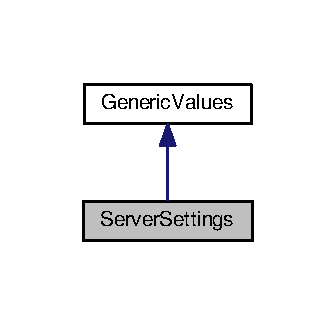
\includegraphics[width=161pt]{classServerSettings__inherit__graph}
\end{center}
\end{figure}


Collaboration diagram for Server\+Settings\+:
\nopagebreak
\begin{figure}[H]
\begin{center}
\leavevmode
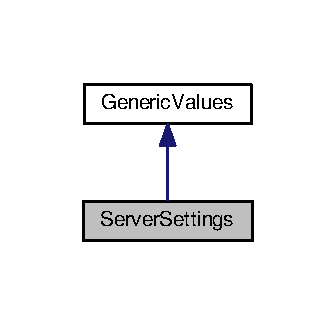
\includegraphics[width=161pt]{classServerSettings__coll__graph}
\end{center}
\end{figure}
\subsection*{Public Member Functions}
\begin{DoxyCompactItemize}
\item 
\hyperlink{classServerSettings_a65be809682094811350d59e690c22831}{Server\+Settings} ()
\item 
bool \hyperlink{classServerSettings_a12701675a372aefe05dfc39c86eb5b12}{set\+Value} (const char $\ast$str\+Name, const char $\ast$str\+Value)
\item 
bool \hyperlink{classServerSettings_aa4bd916ba3cde79d52adc764ee14256f}{read\+Values} (const char $\ast$str\+Filename, const char $\ast$Separator)
\item 
bool \hyperlink{classServerSettings_a60cee781ce0f63a646ec2b6a7696a547}{set\+Goal\+Width} (double d)
\item 
double \hyperlink{classServerSettings_a243427731c0333bc84251c7c305a8b99}{get\+Goal\+Width} () const 
\item 
bool \hyperlink{classServerSettings_ac734b38c5c773d4387132385e2202dc5}{set\+Player\+Size} (double d)
\item 
double \hyperlink{classServerSettings_abbc3b0ef688f88cc27e72d6844759083}{get\+Player\+Size} () const 
\item 
bool \hyperlink{classServerSettings_a688caba9b3229f3548583332e5a9dfdf}{set\+Player\+Decay} (double d)
\item 
double \hyperlink{classServerSettings_a5e7bce215ae06c78d67d232006f06807}{get\+Player\+Decay} () const 
\item 
bool \hyperlink{classServerSettings_a602e1527d12cfbcffbaf348830442d31}{set\+Player\+Rand} (double d)
\item 
double \hyperlink{classServerSettings_a328bdc1051341a09ee05093b4d3ec4e3}{get\+Player\+Rand} () const 
\item 
bool \hyperlink{classServerSettings_a1b2d8a0695235a120111c08f14711b68}{set\+Player\+Weight} (double d)
\item 
double \hyperlink{classServerSettings_a8e03f895c80c32ce4154cd27536d11d1}{get\+Player\+Weight} () const 
\item 
bool \hyperlink{classServerSettings_a4d97721c0b134407b25e55947b4c1da3}{set\+Player\+Speed\+Max} (double d)
\item 
double \hyperlink{classServerSettings_ab3cae216e2ebecb9eab51efade2e6aea}{get\+Player\+Speed\+Max} () const 
\item 
bool \hyperlink{classServerSettings_a043c97bd3a6c3e8a947cabe97631db45}{set\+Player\+Accel\+Max} (double d)
\item 
double \hyperlink{classServerSettings_ab1c0be7e5c6938b9cb14b993a3b96475}{get\+Player\+Accel\+Max} () const 
\item 
bool \hyperlink{classServerSettings_a8fe7848a2ac647e31399aa6165492d7f}{set\+Player\+Speed\+Max\+Min} (double d)
\item 
double \hyperlink{classServerSettings_ae4ef6fc9ecbc172ee962a2c194d628bd}{get\+Player\+Speed\+Max\+Min} () const 
\item 
bool \hyperlink{classServerSettings_ad8ffb5e7b8b18b8b81e24b8f3642c4ff}{set\+Allow\+Mult\+Default\+Type} (bool b)
\item 
bool \hyperlink{classServerSettings_a41fed00325a08851d7c88a28e2073384}{get\+Allow\+Mult\+Default\+Type} () const 
\item 
bool \hyperlink{classServerSettings_a00a4b9f4b20d660d5e6f14a2917fd4a1}{set\+Pt\+Max} (int i)
\item 
int \hyperlink{classServerSettings_a3af477dce65517aec3cb45e4f361885b}{get\+Pt\+Max} () const 
\item 
bool \hyperlink{classServerSettings_a8188fc5312e39dca6f26dc86899124e2}{set\+Stamina\+Max} (double d)
\item 
double \hyperlink{classServerSettings_a8f80b619e0857f510ad63433e74ec336}{get\+Stamina\+Max} () const 
\item 
bool \hyperlink{classServerSettings_ade6fd5e746605152194e12aefacf080a}{set\+Stamina\+Inc\+Max} (double d)
\item 
double \hyperlink{classServerSettings_a2d5ad986fbf61ffff3544141af1f29cd}{get\+Stamina\+Inc\+Max} () const 
\item 
bool \hyperlink{classServerSettings_a5921a4fd7ae7688b1b523b4386a13278}{set\+Recover\+Dec\+Thr} (double d)
\item 
double \hyperlink{classServerSettings_aaef5a1c835f1c88a62d6e968745cc369}{get\+Recover\+Dec\+Thr} () const 
\item 
bool \hyperlink{classServerSettings_ac179b557caeae7994e6fe1d85d9c28cf}{set\+Recover\+Dec} (double d)
\item 
double \hyperlink{classServerSettings_a0c881436c385e3f6a5303731ec2f17a8}{get\+Recover\+Dec} () const 
\item 
bool \hyperlink{classServerSettings_a8bea1fd88a7198e00831c9a2cae00251}{set\+Recover\+Min} (double d)
\item 
double \hyperlink{classServerSettings_a748a52ea5b2eaec27d8cecefbb9a9797}{get\+Recover\+Min} () const 
\item 
bool \hyperlink{classServerSettings_a2a117997fc3df014bfdcb6de4a5fb900}{set\+Effort\+Dec\+Thr} (double d)
\item 
double \hyperlink{classServerSettings_a893754dba565851222cc07837f2eb677}{get\+Effort\+Dec\+Thr} () const 
\item 
bool \hyperlink{classServerSettings_a6adceb77055029c4f935e5b70c864185}{set\+Effort\+Dec} (double d)
\item 
double \hyperlink{classServerSettings_a7f068005fc8d39929081bb4d9f2849a0}{get\+Effort\+Dec} () const 
\item 
bool \hyperlink{classServerSettings_ac2d9af5b8702d95cf47101d20f456ec8}{set\+Effort\+Inc\+Thr} (double d)
\item 
double \hyperlink{classServerSettings_a44bb9d79de2677620f8fd4db0201b2c3}{get\+Effort\+Inc\+Thr} () const 
\item 
bool \hyperlink{classServerSettings_a2339ec254951b15f5acfeff06d7b22a2}{set\+Effort\+Inc} (double d)
\item 
double \hyperlink{classServerSettings_a77b69873f26abdfcbf8564f59be19c50}{get\+Effort\+Inc} () const 
\item 
bool \hyperlink{classServerSettings_a8c2f66a7d2c5619848bb924564a4a5a2}{set\+Effort\+Min} (double d)
\item 
double \hyperlink{classServerSettings_a93d574fac0f46743eb79e49ce4d4fcf2}{get\+Effort\+Min} () const 
\item 
bool \hyperlink{classServerSettings_ac313b6695ef99dc74439f3e5d0d56a73}{set\+Stamina\+Capacity} (double d)
\item 
double \hyperlink{classServerSettings_aac0d2476d085fe056b7033670552e170}{get\+Stamina\+Capacity} () const 
\item 
bool \hyperlink{classServerSettings_a949653e100ea22a093990c895a332a4e}{set\+Hear\+Max} (int i)
\item 
int \hyperlink{classServerSettings_a3e13dc98ccc359583eb774325cdaacda}{get\+Hear\+Max} () const 
\item 
bool \hyperlink{classServerSettings_a08fc847141bf9820c593a9b7c29b1b1d}{set\+Hear\+Inc} (int i)
\item 
int \hyperlink{classServerSettings_a9dca9bb073ad15c88517f7c038611d37}{get\+Hear\+Inc} () const 
\item 
bool \hyperlink{classServerSettings_a9a78fef09f0f231d5def44c2096ae5d1}{set\+Hear\+Decay} (int i)
\item 
int \hyperlink{classServerSettings_aef634b9253fade25b8ae02aa4773338c}{get\+Hear\+Decay} () const 
\item 
bool \hyperlink{classServerSettings_a88b46ac9b950305b86fc0bfe8f145b8e}{set\+Inertia\+Moment} (double d)
\item 
double \hyperlink{classServerSettings_acb21f27205d41a287323d4737e763196}{get\+Inertia\+Moment} () const 
\item 
bool \hyperlink{classServerSettings_a49603fbf8bea502452a2fe2284cc9cb2}{set\+Sense\+Body\+Step} (int i)
\item 
int \hyperlink{classServerSettings_a6a84482c9fcc5b304e2fa41c3eb2e86c}{get\+Sense\+Body\+Step} () const 
\item 
bool \hyperlink{classServerSettings_ab097d1a65525c5851f95507e3d7fa667}{set\+Catchable\+AreaL} (double d)
\item 
double \hyperlink{classServerSettings_acfbe824ae58e9803c8599b3dfbef7622}{get\+Catchable\+AreaL} () const 
\item 
bool \hyperlink{classServerSettings_ade7c654db3622d374e694b13245d9edb}{set\+Catchable\+AreaW} (double d)
\item 
double \hyperlink{classServerSettings_a10896e44a2695024a51b3ff3810f3138}{get\+Catchable\+AreaW} () const 
\item 
bool \hyperlink{classServerSettings_a6f9218ce9e9b4d4d3964be0ffe3f11d6}{set\+Catch\+Probability} (double d)
\item 
double \hyperlink{classServerSettings_a17a67611271faf4b7117b49ba451c0d1}{get\+Catch\+Probability} () const 
\item 
bool \hyperlink{classServerSettings_aaa383bc64b5e6b690d2bbff840fc94e3}{set\+Catch\+Ban\+Cycle} (int i)
\item 
int \hyperlink{classServerSettings_a5524e22ab9bf17d9c24cb2350cf49d27}{get\+Catch\+Ban\+Cycle} () const 
\item 
bool \hyperlink{classServerSettings_ac7340a63321971a2f450bfff00eaa996}{set\+Goalie\+Max\+Moves} (int i)
\item 
int \hyperlink{classServerSettings_a841626ede1c968880e40cb9e18d4e57f}{get\+Goalie\+Max\+Moves} () const 
\item 
bool \hyperlink{classServerSettings_ace618332a7e47d535e150ef73eff5f54}{set\+Ball\+Size} (double d)
\item 
double \hyperlink{classServerSettings_a0a0b193b7d1936ba103f4bd80eb1dd11}{get\+Ball\+Size} () const 
\item 
bool \hyperlink{classServerSettings_ad2f70db19ec4be940be6882dfbd0810b}{set\+Ball\+Decay} (double d)
\item 
double \hyperlink{classServerSettings_a3c15233bbc1e27407eb4bbced64477ad}{get\+Ball\+Decay} () const 
\item 
bool \hyperlink{classServerSettings_a5521e9611b2b224a8e45de337e08cc1d}{set\+Ball\+Rand} (double d)
\item 
double \hyperlink{classServerSettings_a96f93df70f291091044472f9d8398830}{get\+Ball\+Rand} () const 
\item 
bool \hyperlink{classServerSettings_aa8a24da8ae915af2fe8e5b67caefe984}{set\+Ball\+Weight} (double d)
\item 
double \hyperlink{classServerSettings_a7f5f0af2958dbc1d4d17a3d02a794f0e}{get\+Ball\+Weight} () const 
\item 
bool \hyperlink{classServerSettings_a6c7f2ea1d031c9af863ace3a18828448}{set\+Ball\+Speed\+Max} (double d)
\item 
double \hyperlink{classServerSettings_ac8b10c7247665386f572ca9ba658f985}{get\+Ball\+Speed\+Max} () const 
\item 
bool \hyperlink{classServerSettings_a5365e824cf6d761502443a7770d1f9b6}{set\+Ball\+Accel\+Max} (double d)
\item 
double \hyperlink{classServerSettings_a6f49060f4bf6ef0266e79fb28ad9141d}{get\+Ball\+Accel\+Max} () const 
\item 
bool \hyperlink{classServerSettings_a2ada3aeab1c4fc1317190ec9dbc9597f}{set\+Wind\+Force} (double d)
\item 
double \hyperlink{classServerSettings_acf7612afc222e0d244690b3d90951db6}{get\+Wind\+Force} () const 
\item 
bool \hyperlink{classServerSettings_a34644737c9e70c800eda6af9c2b0b3b2}{set\+Wind\+Dir} (double d)
\item 
double \hyperlink{classServerSettings_a682881806da54a4592b55590bcd0be45}{get\+Wind\+Dir} () const 
\item 
bool \hyperlink{classServerSettings_affcdec56bd3bd90d8fe9363e202eba01}{set\+Wind\+Rand} (double d)
\item 
double \hyperlink{classServerSettings_a36d659107a6d0436172e8cee9675035d}{get\+Wind\+Rand} () const 
\item 
bool \hyperlink{classServerSettings_a040608ab561de21a0554d4ecd8bb37d5}{set\+Wind\+Random} (bool b)
\item 
bool \hyperlink{classServerSettings_a4d31b98048b26c549b79f7424a51ea02}{get\+Wind\+Random} () const 
\item 
bool \hyperlink{classServerSettings_a08aec4e5cc2d54619e0821b52394670b}{set\+Kickable\+Margin} (double d)
\item 
double \hyperlink{classServerSettings_a4c944475bec89b0ee7ce9e4d2a5808c0}{get\+Kickable\+Margin} () const 
\item 
bool \hyperlink{classServerSettings_ade913eaa480cead3e496e71a3d16306f}{set\+Ckick\+Margin} (double d)
\item 
double \hyperlink{classServerSettings_a6ddcd85b5129fe16a90ba057b58ab2b1}{get\+Ckick\+Margin} () const 
\item 
bool \hyperlink{classServerSettings_a5a945e55070c1f4c7da35dfd45c05bd2}{set\+Dash\+Power\+Rate} (double d)
\item 
double \hyperlink{classServerSettings_a8c3bc89b83304d506223bdf2c851bd79}{get\+Dash\+Power\+Rate} () const 
\item 
bool \hyperlink{classServerSettings_a5d62744529556cad4276dbb69201e41d}{set\+Kick\+Power\+Rate} (double d)
\item 
double \hyperlink{classServerSettings_a03ac9cca9b81036b4cb23837b28a769c}{get\+Kick\+Power\+Rate} () const 
\item 
bool \hyperlink{classServerSettings_a985e150cf26c4b3690acc7ba206c2c9d}{set\+Kick\+Rand} (double d)
\item 
double \hyperlink{classServerSettings_a6ca6265443dda845dba70024670f5a13}{get\+Kick\+Rand} () const 
\item 
bool \hyperlink{classServerSettings_a94d90a2134e4b2b01635032f26a47426}{set\+Dash\+Angle\+Step} (double d)
\item 
double \hyperlink{classServerSettings_af39faf06d9286d49b5e2ca5b4c03ca22}{get\+Dash\+Angle\+Step} () const 
\item 
bool \hyperlink{classServerSettings_aa8ce2c74656a92ec980574d42b9d7566}{set\+Side\+Dash\+Rate} (double d)
\item 
double \hyperlink{classServerSettings_aae957bd728dde3310f1de707a33642ec}{get\+Side\+Dash\+Rate} () const 
\item 
bool \hyperlink{classServerSettings_a85c7e2f37dfaab959157fa401ee3c02e}{set\+Back\+Dash\+Rate} (double d)
\item 
double \hyperlink{classServerSettings_adb9445b0fcb6e78ad26878c21a666bc1}{get\+Back\+Dash\+Rate} () const 
\item 
bool \hyperlink{classServerSettings_abecc6c28f66e8973bb7b9673efc2ddee}{set\+Visible\+Angle} (double d)
\item 
double \hyperlink{classServerSettings_a963da1f61fdf8145c3ea4b3790d77405}{get\+Visible\+Angle} () const 
\item 
bool \hyperlink{classServerSettings_a7f1a933de1014e9bf2a9d8be0a5a5cc6}{set\+Audio\+Cut\+Dist} (double d)
\item 
double \hyperlink{classServerSettings_ad7b512d77e716b591d0d6dc5a627a931}{get\+Audio\+Cut\+Dist} () const 
\item 
bool \hyperlink{classServerSettings_ac1cb48a9ae349637b6e7dc45eaeef2f3}{set\+Quantize\+Step} (double d)
\item 
double \hyperlink{classServerSettings_ad6b874013ad2ca7ff8f006d4879f70bb}{get\+Quantize\+Step} () const 
\item 
bool \hyperlink{classServerSettings_a689b1cfb84757dc65d442a4d30784b1c}{set\+Quantize\+StepL} (double d)
\item 
double \hyperlink{classServerSettings_a80ef9af63c874229e03350406a764084}{get\+Quantize\+StepL} () const 
\item 
bool \hyperlink{classServerSettings_a55b027ac52d259e891c7458c97fb099d}{set\+Max\+Dash\+Angle} (double i)
\item 
double \hyperlink{classServerSettings_a24b8c5c7951c80607c80afc46549090e}{get\+Max\+Dash\+Angle} () const 
\item 
bool \hyperlink{classServerSettings_a90c50bcf172ceda18b69f9a05115c3ac}{set\+Min\+Dash\+Angle} (double i)
\item 
double \hyperlink{classServerSettings_aeb249707f2c5c9f96f4654a4cd61966b}{get\+Min\+Dash\+Angle} () const 
\item 
bool \hyperlink{classServerSettings_a3ece5159bfb4ef0f633d906fe860e1fe}{set\+Max\+Dash\+Power} (double i)
\item 
double \hyperlink{classServerSettings_a74c696e059ba8e5a1a438d51117c2340}{get\+Max\+Dash\+Power} () const 
\item 
bool \hyperlink{classServerSettings_a3c553f2be24816268404aaf37762d87d}{set\+Min\+Dash\+Power} (double i)
\item 
double \hyperlink{classServerSettings_aaabb8e8d476e9afedac6c9f25efeb726}{get\+Min\+Dash\+Power} () const 
\item 
bool \hyperlink{classServerSettings_a9b40833d34c9953a66b8937dbcb3c8ca}{set\+Max\+Power} (int i)
\item 
int \hyperlink{classServerSettings_ab4c1a2b2555a787d60c3a86c725c3230}{get\+Max\+Power} () const 
\item 
bool \hyperlink{classServerSettings_a677d3c1c82893d16531f01de02fb2d1e}{set\+Min\+Power} (int i)
\item 
int \hyperlink{classServerSettings_a95282be2b593377c0bbcdda56041301f}{get\+Min\+Power} () const 
\item 
bool \hyperlink{classServerSettings_aaa6c80b75827c9b4db6839fa47fe0714}{set\+Max\+Moment} (int i)
\item 
int \hyperlink{classServerSettings_ab04da6dddd31999ab1331f53ba60f4eb}{get\+Max\+Moment} () const 
\item 
bool \hyperlink{classServerSettings_abfb9f165e7803fecd973014ce8a174be}{set\+Min\+Moment} (int i)
\item 
int \hyperlink{classServerSettings_ae16f78bc2d2df91fb22355e8fbb32714}{get\+Min\+Moment} () const 
\item 
bool \hyperlink{classServerSettings_aa712cf5ce1eb2f405a177a28fe58bac3}{set\+Max\+Neck\+Moment} (int i)
\item 
int \hyperlink{classServerSettings_a2123147fd729382d4d8477f07721f4a5}{get\+Max\+Neck\+Moment} () const 
\item 
bool \hyperlink{classServerSettings_a1ec07e04a2e18179ebd88e1c386e472f}{set\+Min\+Neck\+Moment} (int i)
\item 
int \hyperlink{classServerSettings_afe5791e9c4976346dedff56d1b499e7a}{get\+Min\+Neck\+Moment} () const 
\item 
bool \hyperlink{classServerSettings_a86f7a2387351f4703c58268cf4c3f919}{set\+Max\+Neck\+Ang} (int i)
\item 
int \hyperlink{classServerSettings_a255d2d8c5c3de7d995672693381f4574}{get\+Max\+Neck\+Ang} () const 
\item 
bool \hyperlink{classServerSettings_ad071affea570ae510b49aa332eedf7d0}{set\+Min\+Neck\+Ang} (int i)
\item 
int \hyperlink{classServerSettings_a710b861da6c005393452eb87893ccddc}{get\+Min\+Neck\+Ang} () const 
\item 
bool \hyperlink{classServerSettings_a4f9afe067291c05312acaedcb6a46153}{set\+Port} (int i)
\item 
int \hyperlink{classServerSettings_a306ae49f2b66f052ab4a31e3a07f725a}{get\+Port} () const 
\item 
bool \hyperlink{classServerSettings_a5a28c1e193c98556d85b5f2c3ebe649c}{set\+Coach\+Port} (int i)
\item 
int \hyperlink{classServerSettings_a5c25e01f01e6bd6e638489c2b7494a3c}{get\+Coach\+Port} () const 
\item 
bool \hyperlink{classServerSettings_aca252ddb8afa5b62ecc99c56b9b1f83b}{set\+Ol\+Coach\+Port} (int i)
\item 
int \hyperlink{classServerSettings_a3bb63f494c02965a2d35b9ebcf851608}{get\+Ol\+Coach\+Port} () const 
\item 
bool \hyperlink{classServerSettings_aef0db584133e3de82eab8b7831edd012}{set\+Say\+Coach\+Cnt\+Max} (int i)
\item 
int \hyperlink{classServerSettings_afbbe8148cdd6bbd1f71fcfd6d8221c52}{get\+Say\+Coach\+Cnt\+Max} () const 
\item 
bool \hyperlink{classServerSettings_a364676341033fcf84864ff886fab0b80}{set\+Say\+Coach\+Msg\+Size} (int i)
\item 
int \hyperlink{classServerSettings_a3b893e1ff64c7a093f8e7a8aeb2e4c78}{get\+Say\+Coach\+Msg\+Size} () const 
\item 
bool \hyperlink{classServerSettings_a1d946a7ba1e7fb7cd850bf25f63b99a9}{set\+Clang\+Win\+Size} (int i)
\item 
int \hyperlink{classServerSettings_a4e1ee5930596949f0d02ad2da680efd9}{get\+Clang\+Win\+Size} () const 
\item 
bool \hyperlink{classServerSettings_a13b1fbe072e406531db2bef7634ce6f3}{set\+Clang\+Define\+Win} (int i)
\item 
int \hyperlink{classServerSettings_ad4df824d24102f31cbb1bc0589a188ef}{get\+Clang\+Define\+Win} () const 
\item 
bool \hyperlink{classServerSettings_ac1924326862cfd094f2f2dc43f1fdc78}{set\+Clang\+Meta\+Win} (int i)
\item 
int \hyperlink{classServerSettings_ab9d76317f9fd23484388c90a62d47c53}{get\+Clang\+Meta\+Win} () const 
\item 
bool \hyperlink{classServerSettings_a5dbeeca16ae5d2f4edfacd1c6a4667f3}{set\+Clang\+Advice\+Win} (int i)
\item 
int \hyperlink{classServerSettings_a35281fd5711b5fb974ba94769da2424a}{get\+Clang\+Advice\+Win} () const 
\item 
bool \hyperlink{classServerSettings_a766d4d70eee6abdb32f43c1a27df6c94}{set\+Clang\+Info\+Win} (int i)
\item 
int \hyperlink{classServerSettings_a3456116abfedbfde624c25256a2c37f3}{get\+Clang\+Info\+Win} () const 
\item 
bool \hyperlink{classServerSettings_afe7cdd619575361e06d4b060997aa43c}{set\+Clang\+Mess\+Delay} (int i)
\item 
int \hyperlink{classServerSettings_a4dc545d36594f05922fc8e61514cb606}{get\+Clang\+Mess\+Delay} () const 
\item 
bool \hyperlink{classServerSettings_a9e605b177fb5c414dbf59084c5ec5e10}{set\+Clang\+Mess\+Per\+Cycle} (int i)
\item 
int \hyperlink{classServerSettings_a27380257213628762091c93d58390948}{get\+Clang\+Mess\+Per\+Cycle} () const 
\item 
bool \hyperlink{classServerSettings_a088043491ed1bc03040dd887ad5f47e1}{set\+Send\+Vi\+Step} (int i)
\item 
int \hyperlink{classServerSettings_aaa32ec6cb242077d05df626c84781445}{get\+Send\+Vi\+Step} () const 
\item 
bool \hyperlink{classServerSettings_a2869c05d50f4ef6d6204c0ec8ca3b59e}{set\+Simulator\+Step} (int i)
\item 
int \hyperlink{classServerSettings_a9500227b5ccc6d94fd6b3d7e6b36695e}{get\+Simulator\+Step} () const 
\item 
bool \hyperlink{classServerSettings_ac602b593363e8541929e4f7918b90588}{set\+Send\+Step} (int i)
\item 
int \hyperlink{classServerSettings_a0320ba9547d7a54d48d22eb74b993f21}{get\+Send\+Step} () const 
\item 
bool \hyperlink{classServerSettings_a1a9f458b7f01ee56d0f80226d9dc3f39}{set\+Recv\+Step} (int i)
\item 
int \hyperlink{classServerSettings_a4ef829c05858d96172f7553e877954e7}{get\+Recv\+Step} () const 
\item 
bool \hyperlink{classServerSettings_a3ed08dbc57467699cca28e5df55c87c1}{set\+Half\+Time} (int i)
\item 
int \hyperlink{classServerSettings_a36e248356e280136039977eb04e7ca96}{get\+Half\+Time} () const 
\item 
bool \hyperlink{classServerSettings_a62e5564cbcb446a58f7f308f765c0c16}{set\+Drop\+Ball\+Time} (int i)
\item 
int \hyperlink{classServerSettings_a8c79e76c186c51c64e856ebfa1d5af32}{get\+Drop\+Ball\+Time} () const 
\item 
bool \hyperlink{classServerSettings_ae1f80bf2138edc9caa65f6adb3c0bc49}{set\+Extra\+Half\+Time} (int i)
\item 
int \hyperlink{classServerSettings_a1ec8e7e51fbbdc6f81a7fd9d142998ea}{get\+Extra\+Half\+Time} () const 
\item 
bool \hyperlink{classServerSettings_a3f05df809345b0b22aef3268effa213c}{set\+Say\+Msg\+Size} (int i)
\item 
int \hyperlink{classServerSettings_a84d032cebb7961efe59ad79365ff5731}{get\+Say\+Msg\+Size} () const 
\item 
bool \hyperlink{classServerSettings_a37fc1b150b744608c9263112f7fcaecb}{set\+Use\+Offside} (bool b)
\item 
bool \hyperlink{classServerSettings_a0d6e9968399d5c07aac912615eccc5c7}{get\+Use\+Offside} () const 
\item 
bool \hyperlink{classServerSettings_a91fe86f0a25411b67c35974872d1bcfe}{set\+Offside\+Active\+Area\+Size} (double d)
\item 
double \hyperlink{classServerSettings_ac72bd2dc946a31d4ab5688263f39fc36}{get\+Offside\+Active\+Area\+Size} () const 
\item 
bool \hyperlink{classServerSettings_a6acffd58c850f6870cbbc60b04f6d77f}{set\+Forbid\+Kick\+Off\+Offside} (bool b)
\item 
bool \hyperlink{classServerSettings_ac58e50ab3445d43a41c10a3f654ac349}{get\+Forbid\+Kick\+Off\+Offside} () const 
\item 
bool \hyperlink{classServerSettings_a2575a4a97478ba34bf40e7b1ef776502}{set\+Offside\+Kick\+Margin} (double d)
\item 
double \hyperlink{classServerSettings_ac9c5d2d3786da204c2932229f536a47f}{get\+Offside\+Kick\+Margin} () const 
\item 
bool \hyperlink{classServerSettings_add8bbf7b3915098d544dd6aa36a34380}{set\+Verbose} (bool b)
\item 
bool \hyperlink{classServerSettings_a7366fa584c5ddd63e3a8afd0ac2c3da2}{get\+Verbose} () const 
\item 
bool \hyperlink{classServerSettings_a24b88ba444bab9d41ca23dd175993a61}{set\+Record\+Version} (int i)
\item 
int \hyperlink{classServerSettings_aff2312687e28b90cac35fa6b97161757}{get\+Record\+Version} () const 
\item 
bool \hyperlink{classServerSettings_aade52919304fcf81331dad3ac221c072}{set\+Record\+Log} (bool b)
\item 
bool \hyperlink{classServerSettings_ac2ad8593d56dc8791550e5ac678365dd}{get\+Record\+Log} () const 
\item 
bool \hyperlink{classServerSettings_ad39466625b0f21bcf8a509fb22e7c694}{set\+Send\+Log} (bool b)
\item 
bool \hyperlink{classServerSettings_a3d56bffd30bab022ea3b56768cbb03dc}{get\+Send\+Log} () const 
\item 
bool \hyperlink{classServerSettings_adada5579b234820ef3965c193a3cd07b}{set\+Log\+Times} (bool b)
\item 
bool \hyperlink{classServerSettings_a2fe5ce14ebe2d520b3bbbc3980c7b2c8}{get\+Log\+Times} () const 
\item 
bool \hyperlink{classServerSettings_a3a1fc8f8e22ac5c066d447fcbeb932d2}{set\+Log\+File} (char $\ast$str)
\item 
char $\ast$ \hyperlink{classServerSettings_a33856b4ce798a30ebcc2484980c22ab6}{get\+Log\+File} ()
\item 
bool \hyperlink{classServerSettings_a0c0ce0ac89c3243f7658b7262826b8c2}{set\+Synch\+Mode} (bool b)
\item 
bool \hyperlink{classServerSettings_a5e4741b63584e17556dd624221cf94e9}{get\+Synch\+Mode} () const 
\item 
bool \hyperlink{classServerSettings_a2b410587fb81822521cdbbbeed3fe4ee}{set\+Full\+State\+Left} (bool b)
\item 
bool \hyperlink{classServerSettings_a52b032d71c2d87c82cc9753dbd8cb568}{get\+Full\+State\+Left} () const 
\item 
bool \hyperlink{classServerSettings_a1d9cc6cfe1ba3de09f7fab7d2277cc2b}{set\+Full\+State\+Right} (bool b)
\item 
bool \hyperlink{classServerSettings_a59006e348c5bf744aacdf5eae8af85c8}{get\+Full\+State\+Right} () const 
\item 
bool \hyperlink{classServerSettings_af4601c1d32690d2bc23200b7bd39d56d}{set\+Player\+Types} (int i)
\item 
int \hyperlink{classServerSettings_a3ea2d972b477489f16f9044e77b33517}{get\+Player\+Types} () const 
\item 
bool \hyperlink{classServerSettings_ab270bf7eef5016ebaf6aeb9e3b4d7680}{set\+Subs\+Max} (int i)
\item 
int \hyperlink{classServerSettings_a9a8e99334d23099191cef30be2a365d9}{get\+Subs\+Max} () const 
\item 
bool \hyperlink{classServerSettings_a732188ae4d8068768a4974e5e09e7d91}{set\+Player\+Speed\+Max\+Delta\+Min} (double d)
\item 
double \hyperlink{classServerSettings_ab2358daa4b23f1f2342f23f76b466af8}{get\+Player\+Speed\+Max\+Delta\+Min} () const 
\item 
bool \hyperlink{classServerSettings_acfdafdeacd1d291d7aeaa145cc3610dd}{set\+Player\+Speed\+Max\+Delta\+Max} (double d)
\item 
double \hyperlink{classServerSettings_a8fb5c7b85dcec6f05702c6284ff4bd45}{get\+Player\+Speed\+Max\+Delta\+Max} () const 
\item 
bool \hyperlink{classServerSettings_a8b4aa98bda2350c35e35748b33c1880f}{set\+Stamina\+Inc\+Max\+Delta\+Factor} (double d)
\item 
double \hyperlink{classServerSettings_a74cd1e116075a58d218dc802943e4071}{get\+Stamina\+Inc\+Max\+Delta\+Factor} () const 
\item 
bool \hyperlink{classServerSettings_a6d7e9f12ce219523ac94a547a06c8330}{set\+Player\+Decay\+Delta\+Min} (double d)
\item 
double \hyperlink{classServerSettings_a5b4d8a4bb803df8428d89e01a64e1bfb}{get\+Player\+Decay\+Delta\+Min} () const 
\item 
bool \hyperlink{classServerSettings_a103639801cc6c13662ec4e0b6ed0ec0b}{set\+Player\+Decay\+Delta\+Max} (double d)
\item 
double \hyperlink{classServerSettings_affdfc06e62a638d64ffc95c3fd559a9d}{get\+Player\+Decay\+Delta\+Max} () const 
\item 
bool \hyperlink{classServerSettings_aed5d249aea08850f0f0aef19efec9ce3}{set\+Inertia\+Moment\+Delta\+Factor} (double d)
\item 
double \hyperlink{classServerSettings_a6da6f800cc36c70ec191f239a8818b87}{get\+Inertia\+Moment\+Delta\+Factor} () const 
\item 
bool \hyperlink{classServerSettings_ade566764abe2366ff29acd6eb2a97676}{set\+Dash\+Power\+Rate\+Delta\+Min} (double d)
\item 
double \hyperlink{classServerSettings_aa2b26db481ea52080318a0045aed14bd}{get\+Dash\+Power\+Rate\+Delta\+Min} () const 
\item 
bool \hyperlink{classServerSettings_a05731d8156482a76b800ef242341d49a}{set\+Dash\+Power\+Rate\+Delta\+Max} (double d)
\item 
double \hyperlink{classServerSettings_ae561ab94c78a5df974269f757008d140}{get\+Dash\+Power\+Rate\+Delta\+Max} () const 
\item 
bool \hyperlink{classServerSettings_ac7ae5d47d3763512df27a7ae0e6eac5d}{set\+Player\+Size\+Delta\+Factor} (double d)
\item 
double \hyperlink{classServerSettings_a8913804089359b0dd41d5bef87330995}{get\+Player\+Size\+Delta\+Factor} () const 
\item 
bool \hyperlink{classServerSettings_a6ae37cf80edc57f457f7d946b3c91638}{set\+Kickable\+Margin\+Delta\+Min} (double d)
\item 
double \hyperlink{classServerSettings_a7a055d4565837966f2d278d2b1dbc988}{get\+Kickable\+Margin\+Delta\+Min} () const 
\item 
bool \hyperlink{classServerSettings_a99d5f31b575c976b289a5a0e7a185b24}{set\+Kickable\+Margin\+Delta\+Max} (double d)
\item 
double \hyperlink{classServerSettings_acf96251b45264e562b111a8cb6bc17f0}{get\+Kickable\+Margin\+Delta\+Max} () const 
\item 
bool \hyperlink{classServerSettings_aa63a5ea0705aaa18d7ab8b00752ca744}{set\+Kick\+Rand\+Delta\+Factor} (double d)
\item 
double \hyperlink{classServerSettings_a5f6694b556bb82c0e4f288f2680af399}{get\+Kick\+Rand\+Delta\+Factor} () const 
\item 
bool \hyperlink{classServerSettings_ad5fbafa4026c2c81bacaf588dd4d3b8b}{set\+Extra\+Stamina\+Delta\+Min} (double d)
\item 
double \hyperlink{classServerSettings_acf2beb30b73d2488b6227b6f323bc716}{get\+Extra\+Stamina\+Delta\+Min} () const 
\item 
bool \hyperlink{classServerSettings_aa672ed84f340a7516e2bbed2c74e336a}{set\+Extra\+Stamina\+Delta\+Max} (double d)
\item 
double \hyperlink{classServerSettings_af04f8ef0354a17fe981a6cf69ae7b8b6}{get\+Extra\+Stamina\+Delta\+Max} () const 
\item 
bool \hyperlink{classServerSettings_ae59b47a83a58668b4ad2bd46b5b7d3df}{set\+Effort\+Max\+Delta\+Factor} (double d)
\item 
double \hyperlink{classServerSettings_a6a8d9120c34b43910f7620841e4000cf}{get\+Effort\+Max\+Delta\+Factor} () const 
\item 
bool \hyperlink{classServerSettings_a8970efdf9782d2896e5dd718d6d094a1}{set\+Effort\+Min\+Delta\+Factor} (double d)
\item 
double \hyperlink{classServerSettings_a352b24e33ccbc7be3330d7af2c852e6c}{get\+Effort\+Min\+Delta\+Factor} () const 
\item 
bool \hyperlink{classServerSettings_a77958b0b18db2177d5f25ec12e6a9ed1}{set\+New\+Dash\+Power\+Rate\+Delta\+Min} (double d)
\item 
double \hyperlink{classServerSettings_aad1659c992f6893a51fda7c8ce36fc93}{get\+New\+Dash\+Power\+Rate\+Delta\+Min} () const 
\item 
bool \hyperlink{classServerSettings_a3ff4672fd3702001162dfc3f7e139431}{set\+New\+Dash\+Power\+Rate\+Delta\+Max} (double d)
\item 
double \hyperlink{classServerSettings_a4942128c18070883debd4bde229c650a}{get\+New\+Dash\+Power\+Rate\+Delta\+Max} () const 
\item 
bool \hyperlink{classServerSettings_aeb922be1a2b91caa13447ffe7647a174}{set\+New\+Stamina\+Inc\+Max\+Delta\+Factor} (double d)
\item 
double \hyperlink{classServerSettings_a8865c04b5238507a04d979461cf05cc1}{get\+New\+Stamina\+Inc\+Max\+Delta\+Factor} () const 
\item 
bool \hyperlink{classServerSettings_a5f9d08c5393ce55c72616e265d5beba3}{set\+Pen\+DistX} (double d)
\item 
double \hyperlink{classServerSettings_af5db055dcbfdfb35de09c2c365891636}{get\+Pen\+DistX} () const 
\item 
bool \hyperlink{classServerSettings_a8e04b3db869ea61330d4bb807d658be3}{set\+Pen\+Max\+Goalie\+DistX} (double d)
\item 
double \hyperlink{classServerSettings_ac43b5188bb72420b5294bb041de47a45}{get\+Pen\+Max\+Goalie\+DistX} () const 
\item 
bool \hyperlink{classServerSettings_a5aaaafc1c31a33e661b0d2b1ea7be2b3}{set\+Pen\+Allow\+Mult\+Kicks} (bool b)
\item 
bool \hyperlink{classServerSettings_a5da97d527638da8c9b9e43b05a37d392}{get\+Pen\+Allow\+Mult\+Kicks} () const 
\item 
bool {\bfseries set\+Pen\+Max\+Extra\+Kicks} (int i)\hypertarget{classServerSettings_a80943011afc16fbdf1078bc3cb2e7769}{}\label{classServerSettings_a80943011afc16fbdf1078bc3cb2e7769}

\item 
int {\bfseries get\+Pen\+Max\+Extra\+Kicks} () const \hypertarget{classServerSettings_a59c561b78fab635ff47910d7b8499e84}{}\label{classServerSettings_a59c561b78fab635ff47910d7b8499e84}

\item 
bool {\bfseries set\+Pen\+Before\+Setup\+Wait} (int i)\hypertarget{classServerSettings_a4ab588988b7a44eaabd296e129e718c5}{}\label{classServerSettings_a4ab588988b7a44eaabd296e129e718c5}

\item 
int {\bfseries get\+Pen\+Before\+Setup\+Wait} () const \hypertarget{classServerSettings_a66b99d1a390ad09875dff4a83034a430}{}\label{classServerSettings_a66b99d1a390ad09875dff4a83034a430}

\item 
bool {\bfseries set\+Pen\+Ready\+Wait} (int i)\hypertarget{classServerSettings_a7f19de6401a51f4fbb81af21e82d0904}{}\label{classServerSettings_a7f19de6401a51f4fbb81af21e82d0904}

\item 
int {\bfseries get\+Pen\+Ready\+Wait} () const \hypertarget{classServerSettings_ae683f4cb31425963cc7812f0a9849523}{}\label{classServerSettings_ae683f4cb31425963cc7812f0a9849523}

\item 
bool {\bfseries set\+Pen\+Setup\+Wait} (int i)\hypertarget{classServerSettings_a50a8d6545918f92c30c8bde8450940c6}{}\label{classServerSettings_a50a8d6545918f92c30c8bde8450940c6}

\item 
int {\bfseries get\+Pen\+Setup\+Wait} () const \hypertarget{classServerSettings_a90717ee81afabd098ff32ebfbc3c6f9f}{}\label{classServerSettings_a90717ee81afabd098ff32ebfbc3c6f9f}

\item 
bool {\bfseries set\+Pen\+Taken\+Wait} (int i)\hypertarget{classServerSettings_a1b35ffa095683369a368ae6b187a76f3}{}\label{classServerSettings_a1b35ffa095683369a368ae6b187a76f3}

\item 
int {\bfseries get\+Pen\+Taken\+Wait} () const \hypertarget{classServerSettings_a59a2a711ef3fa1434d39d153fa305615}{}\label{classServerSettings_a59a2a711ef3fa1434d39d153fa305615}

\item 
bool \hyperlink{classServerSettings_afc7ff765cf6dd3940cd839c98a49384b}{set\+Tackle\+Dist} (double d)
\item 
double \hyperlink{classServerSettings_af3a8871883dfd17428fd5cf0e5be29e5}{get\+Tackle\+Dist} () const 
\item 
bool \hyperlink{classServerSettings_a4db5b82416c075b8c848c1d08dbb03aa}{set\+Tackle\+Back\+Dist} (double d)
\item 
double \hyperlink{classServerSettings_a0b93d810c1367f09c72d767c5b1c9ede}{get\+Tackle\+Back\+Dist} () const 
\item 
bool \hyperlink{classServerSettings_a56db9e44287ad34d288dc779dff4946f}{set\+Tackle\+Width} (double d)
\item 
double \hyperlink{classServerSettings_a0a4553abb2f0eba3fd6d522e026e1434}{get\+Tackle\+Width} () const 
\item 
bool \hyperlink{classServerSettings_a3137d20ebc1cc883cb05c809ff065135}{set\+Tackle\+Exponent} (double d)
\item 
double \hyperlink{classServerSettings_a1a27fc1e673da5fa4c24bac23a973a07}{get\+Tackle\+Exponent} () const 
\item 
bool \hyperlink{classServerSettings_aec8837f6609b394c8d93bbe3290a8d08}{set\+Tackle\+Cycles} (int i)
\item 
int \hyperlink{classServerSettings_aa09836ed36a8aa91555a2924802af6f2}{get\+Tackle\+Cycles} () const 
\item 
bool \hyperlink{classServerSettings_a1e2a3d629c4413ac87581b438e379ae2}{set\+Tackle\+Power\+Rate} (double d)
\item 
double \hyperlink{classServerSettings_a67bd8680bbab8c242a6ebe662d93f73d}{get\+Tackle\+Power\+Rate} () const 
\item 
bool {\bfseries set\+Max\+Back\+Tackle\+Power} (double d)\hypertarget{classServerSettings_af41df6c5b4efaa504163e1cd7df2f6df}{}\label{classServerSettings_af41df6c5b4efaa504163e1cd7df2f6df}

\item 
double {\bfseries get\+Max\+Back\+Tackle\+Power} () const \hypertarget{classServerSettings_ae790a11cc35650fa33802d6a6d01884e}{}\label{classServerSettings_ae790a11cc35650fa33802d6a6d01884e}

\item 
bool {\bfseries set\+Max\+Tackle\+Power} (double d)\hypertarget{classServerSettings_acb4d369d51360ed9de9b000779392497}{}\label{classServerSettings_acb4d369d51360ed9de9b000779392497}

\item 
double {\bfseries get\+Max\+Tackle\+Power} () const \hypertarget{classServerSettings_a12b8bd1281e041915a1c38a9fa4cd80f}{}\label{classServerSettings_a12b8bd1281e041915a1c38a9fa4cd80f}

\item 
bool \hyperlink{classServerSettings_a6ba0242ad271bef0a6dc8bdbaedca21c}{set\+Effort\+Max} (double d)
\item 
double \hyperlink{classServerSettings_a85a4630574356df9699acde5d301219a}{get\+Effort\+Max} () const 
\item 
bool \hyperlink{classServerSettings_a1b2850fc9560f80077db4f8ad8649551}{set\+Slow\+Down\+Factor} (int i)
\item 
int \hyperlink{classServerSettings_a5a0910122c8f615000415028de44486a}{get\+Slow\+Down\+Factor} () const 
\item 
bool \hyperlink{classServerSettings_a64a83991ccddb3376afe4058b34b54ed}{set\+Visible\+Distance} (double d)
\item 
double \hyperlink{classServerSettings_a88b3758c43e7d6f5b262adea2a1c5377}{get\+Visible\+Distance} () const 
\item 
bool \hyperlink{classServerSettings_aa218d1b32cd7a4f4542d0fc4c0febb1c}{set\+Extra\+Stamina} (double d)
\item 
double \hyperlink{classServerSettings_a2e11ef6c20c038fe9efdd3365107109e}{get\+Extra\+Stamina} () const 
\item 
bool \hyperlink{classServerSettings_a165f3c5d847ff5d089bb3f9b3ed533a0}{set\+Maximal\+Kick\+Dist} (double d)
\item 
double \hyperlink{classServerSettings_af2efd28299ebf01ef1838065e78ebfac}{get\+Maximal\+Kick\+Dist} () const 
\end{DoxyCompactItemize}


\subsection{Detailed Description}
This class contains all the Soccerserver parameters that are available in the configuration file \textquotesingle{}server.\+conf\textquotesingle{} along with their default values and standard set-\/ and get methods for manipulating these values. The \hyperlink{classServerSettings}{Server\+Settings} class is a subclass of the \hyperlink{classGenericValues}{Generic\+Values} class and therefore each value in this class can be reached through the string name of the corresponding parameter. 

\subsection{Constructor \& Destructor Documentation}
\index{Server\+Settings@{Server\+Settings}!Server\+Settings@{Server\+Settings}}
\index{Server\+Settings@{Server\+Settings}!Server\+Settings@{Server\+Settings}}
\subsubsection[{\texorpdfstring{Server\+Settings()}{ServerSettings()}}]{\setlength{\rightskip}{0pt plus 5cm}Server\+Settings\+::\+Server\+Settings (
\begin{DoxyParamCaption}
{}
\end{DoxyParamCaption}
)}\hypertarget{classServerSettings_a65be809682094811350d59e690c22831}{}\label{classServerSettings_a65be809682094811350d59e690c22831}
Constructor for the \hyperlink{classServerSettings}{Server\+Settings} class. It sets all the private member variables in this class to the values specified in the configuration files (server.\+conf and player.\+conf) of Soccer Server version 8.\+xx. These values can be changed by calling the method \textquotesingle{}read\+Values\textquotesingle{} with a new configuration file or by calling the method \textquotesingle{}set\+Value\textquotesingle{} for a specific variable. 

\subsection{Member Function Documentation}
\index{Server\+Settings@{Server\+Settings}!get\+Allow\+Mult\+Default\+Type@{get\+Allow\+Mult\+Default\+Type}}
\index{get\+Allow\+Mult\+Default\+Type@{get\+Allow\+Mult\+Default\+Type}!Server\+Settings@{Server\+Settings}}
\subsubsection[{\texorpdfstring{get\+Allow\+Mult\+Default\+Type() const }{getAllowMultDefaultType() const }}]{\setlength{\rightskip}{0pt plus 5cm}bool Server\+Settings\+::get\+Allow\+Mult\+Default\+Type (
\begin{DoxyParamCaption}
{}
\end{DoxyParamCaption}
) const}\hypertarget{classServerSettings_a41fed00325a08851d7c88a28e2073384}{}\label{classServerSettings_a41fed00325a08851d7c88a28e2073384}
Get method for the \textquotesingle{}d\+Allow\+Mult\+Default\+Type\textquotesingle{} member variable. \begin{DoxyReturn}{Returns}
the use of more than one player default is permitted 
\end{DoxyReturn}
\index{Server\+Settings@{Server\+Settings}!get\+Audio\+Cut\+Dist@{get\+Audio\+Cut\+Dist}}
\index{get\+Audio\+Cut\+Dist@{get\+Audio\+Cut\+Dist}!Server\+Settings@{Server\+Settings}}
\subsubsection[{\texorpdfstring{get\+Audio\+Cut\+Dist() const }{getAudioCutDist() const }}]{\setlength{\rightskip}{0pt plus 5cm}double Server\+Settings\+::get\+Audio\+Cut\+Dist (
\begin{DoxyParamCaption}
{}
\end{DoxyParamCaption}
) const}\hypertarget{classServerSettings_ad7b512d77e716b591d0d6dc5a627a931}{}\label{classServerSettings_ad7b512d77e716b591d0d6dc5a627a931}
Get method for the \textquotesingle{}d\+Audio\+Cut\+Dist\textquotesingle{} member variable. \begin{DoxyReturn}{Returns}
the maximum distance over which a spoken message can be heard 
\end{DoxyReturn}
\index{Server\+Settings@{Server\+Settings}!get\+Back\+Dash\+Rate@{get\+Back\+Dash\+Rate}}
\index{get\+Back\+Dash\+Rate@{get\+Back\+Dash\+Rate}!Server\+Settings@{Server\+Settings}}
\subsubsection[{\texorpdfstring{get\+Back\+Dash\+Rate() const }{getBackDashRate() const }}]{\setlength{\rightskip}{0pt plus 5cm}double Server\+Settings\+::get\+Back\+Dash\+Rate (
\begin{DoxyParamCaption}
{}
\end{DoxyParamCaption}
) const}\hypertarget{classServerSettings_adb9445b0fcb6e78ad26878c21a666bc1}{}\label{classServerSettings_adb9445b0fcb6e78ad26878c21a666bc1}
Get method for the \textquotesingle{}d\+Back\+Dash\+Rate\textquotesingle{} member variable. \begin{DoxyReturn}{Returns}
the the rate by which the \textquotesingle{}Power\textquotesingle{}argument in a backward \textquotesingle{}dash\textquotesingle{} command is multiplied 
\end{DoxyReturn}
\index{Server\+Settings@{Server\+Settings}!get\+Ball\+Accel\+Max@{get\+Ball\+Accel\+Max}}
\index{get\+Ball\+Accel\+Max@{get\+Ball\+Accel\+Max}!Server\+Settings@{Server\+Settings}}
\subsubsection[{\texorpdfstring{get\+Ball\+Accel\+Max() const }{getBallAccelMax() const }}]{\setlength{\rightskip}{0pt plus 5cm}double Server\+Settings\+::get\+Ball\+Accel\+Max (
\begin{DoxyParamCaption}
{}
\end{DoxyParamCaption}
) const}\hypertarget{classServerSettings_a6f49060f4bf6ef0266e79fb28ad9141d}{}\label{classServerSettings_a6f49060f4bf6ef0266e79fb28ad9141d}
Get method for the \textquotesingle{}d\+Ball\+Accel\+Max\textquotesingle{} member variable. \begin{DoxyReturn}{Returns}
the maximum acceleration of the ball per cycle 
\end{DoxyReturn}
\index{Server\+Settings@{Server\+Settings}!get\+Ball\+Decay@{get\+Ball\+Decay}}
\index{get\+Ball\+Decay@{get\+Ball\+Decay}!Server\+Settings@{Server\+Settings}}
\subsubsection[{\texorpdfstring{get\+Ball\+Decay() const }{getBallDecay() const }}]{\setlength{\rightskip}{0pt plus 5cm}double Server\+Settings\+::get\+Ball\+Decay (
\begin{DoxyParamCaption}
{}
\end{DoxyParamCaption}
) const}\hypertarget{classServerSettings_a3c15233bbc1e27407eb4bbced64477ad}{}\label{classServerSettings_a3c15233bbc1e27407eb4bbced64477ad}
Get method for the \textquotesingle{}d\+Ball\+Decay\textquotesingle{} member variable. \begin{DoxyReturn}{Returns}
the ball speed decay per cycle 
\end{DoxyReturn}
\index{Server\+Settings@{Server\+Settings}!get\+Ball\+Rand@{get\+Ball\+Rand}}
\index{get\+Ball\+Rand@{get\+Ball\+Rand}!Server\+Settings@{Server\+Settings}}
\subsubsection[{\texorpdfstring{get\+Ball\+Rand() const }{getBallRand() const }}]{\setlength{\rightskip}{0pt plus 5cm}double Server\+Settings\+::get\+Ball\+Rand (
\begin{DoxyParamCaption}
{}
\end{DoxyParamCaption}
) const}\hypertarget{classServerSettings_a96f93df70f291091044472f9d8398830}{}\label{classServerSettings_a96f93df70f291091044472f9d8398830}
Get method for the \textquotesingle{}d\+Ball\+Rand\textquotesingle{} member variable. \begin{DoxyReturn}{Returns}
the random error in the ball movement 
\end{DoxyReturn}
\index{Server\+Settings@{Server\+Settings}!get\+Ball\+Size@{get\+Ball\+Size}}
\index{get\+Ball\+Size@{get\+Ball\+Size}!Server\+Settings@{Server\+Settings}}
\subsubsection[{\texorpdfstring{get\+Ball\+Size() const }{getBallSize() const }}]{\setlength{\rightskip}{0pt plus 5cm}double Server\+Settings\+::get\+Ball\+Size (
\begin{DoxyParamCaption}
{}
\end{DoxyParamCaption}
) const}\hypertarget{classServerSettings_a0a0b193b7d1936ba103f4bd80eb1dd11}{}\label{classServerSettings_a0a0b193b7d1936ba103f4bd80eb1dd11}
Get method for the \textquotesingle{}d\+Ball\+Size\textquotesingle{} member variable. \begin{DoxyReturn}{Returns}
the size (=radius) of the ball 
\end{DoxyReturn}
\index{Server\+Settings@{Server\+Settings}!get\+Ball\+Speed\+Max@{get\+Ball\+Speed\+Max}}
\index{get\+Ball\+Speed\+Max@{get\+Ball\+Speed\+Max}!Server\+Settings@{Server\+Settings}}
\subsubsection[{\texorpdfstring{get\+Ball\+Speed\+Max() const }{getBallSpeedMax() const }}]{\setlength{\rightskip}{0pt plus 5cm}double Server\+Settings\+::get\+Ball\+Speed\+Max (
\begin{DoxyParamCaption}
{}
\end{DoxyParamCaption}
) const}\hypertarget{classServerSettings_ac8b10c7247665386f572ca9ba658f985}{}\label{classServerSettings_ac8b10c7247665386f572ca9ba658f985}
Get method for the \textquotesingle{}d\+Ball\+Speed\+Max\textquotesingle{} member variable. \begin{DoxyReturn}{Returns}
the maximum speed of the ball 
\end{DoxyReturn}
\index{Server\+Settings@{Server\+Settings}!get\+Ball\+Weight@{get\+Ball\+Weight}}
\index{get\+Ball\+Weight@{get\+Ball\+Weight}!Server\+Settings@{Server\+Settings}}
\subsubsection[{\texorpdfstring{get\+Ball\+Weight() const }{getBallWeight() const }}]{\setlength{\rightskip}{0pt plus 5cm}double Server\+Settings\+::get\+Ball\+Weight (
\begin{DoxyParamCaption}
{}
\end{DoxyParamCaption}
) const}\hypertarget{classServerSettings_a7f5f0af2958dbc1d4d17a3d02a794f0e}{}\label{classServerSettings_a7f5f0af2958dbc1d4d17a3d02a794f0e}
Get method for the \textquotesingle{}d\+Ball\+Weight\textquotesingle{} member variable. \begin{DoxyReturn}{Returns}
the weight of the ball (for wind) 
\end{DoxyReturn}
\index{Server\+Settings@{Server\+Settings}!get\+Catchable\+AreaL@{get\+Catchable\+AreaL}}
\index{get\+Catchable\+AreaL@{get\+Catchable\+AreaL}!Server\+Settings@{Server\+Settings}}
\subsubsection[{\texorpdfstring{get\+Catchable\+Area\+L() const }{getCatchableAreaL() const }}]{\setlength{\rightskip}{0pt plus 5cm}double Server\+Settings\+::get\+Catchable\+AreaL (
\begin{DoxyParamCaption}
{}
\end{DoxyParamCaption}
) const}\hypertarget{classServerSettings_acfbe824ae58e9803c8599b3dfbef7622}{}\label{classServerSettings_acfbe824ae58e9803c8599b3dfbef7622}
Get method for the \textquotesingle{}d\+Catchable\+AreaL\textquotesingle{} member variable. \begin{DoxyReturn}{Returns}
the length of the area around the goalkeeper in which he can catch the ball 
\end{DoxyReturn}
\index{Server\+Settings@{Server\+Settings}!get\+Catchable\+AreaW@{get\+Catchable\+AreaW}}
\index{get\+Catchable\+AreaW@{get\+Catchable\+AreaW}!Server\+Settings@{Server\+Settings}}
\subsubsection[{\texorpdfstring{get\+Catchable\+Area\+W() const }{getCatchableAreaW() const }}]{\setlength{\rightskip}{0pt plus 5cm}double Server\+Settings\+::get\+Catchable\+AreaW (
\begin{DoxyParamCaption}
{}
\end{DoxyParamCaption}
) const}\hypertarget{classServerSettings_a10896e44a2695024a51b3ff3810f3138}{}\label{classServerSettings_a10896e44a2695024a51b3ff3810f3138}
Get method for the \textquotesingle{}d\+Catchable\+AreaW\textquotesingle{} member variable. \begin{DoxyReturn}{Returns}
the width of the area around the goalkeeper in which he can catch the ball 
\end{DoxyReturn}
\index{Server\+Settings@{Server\+Settings}!get\+Catch\+Ban\+Cycle@{get\+Catch\+Ban\+Cycle}}
\index{get\+Catch\+Ban\+Cycle@{get\+Catch\+Ban\+Cycle}!Server\+Settings@{Server\+Settings}}
\subsubsection[{\texorpdfstring{get\+Catch\+Ban\+Cycle() const }{getCatchBanCycle() const }}]{\setlength{\rightskip}{0pt plus 5cm}int Server\+Settings\+::get\+Catch\+Ban\+Cycle (
\begin{DoxyParamCaption}
{}
\end{DoxyParamCaption}
) const}\hypertarget{classServerSettings_a5524e22ab9bf17d9c24cb2350cf49d27}{}\label{classServerSettings_a5524e22ab9bf17d9c24cb2350cf49d27}
Get method for the \textquotesingle{}i\+Catch\+Ban\+Cycle\textquotesingle{} member variable. \begin{DoxyReturn}{Returns}
the number of cycles after a catch in which the goalkeeper cannot catch again 
\end{DoxyReturn}
\index{Server\+Settings@{Server\+Settings}!get\+Catch\+Probability@{get\+Catch\+Probability}}
\index{get\+Catch\+Probability@{get\+Catch\+Probability}!Server\+Settings@{Server\+Settings}}
\subsubsection[{\texorpdfstring{get\+Catch\+Probability() const }{getCatchProbability() const }}]{\setlength{\rightskip}{0pt plus 5cm}double Server\+Settings\+::get\+Catch\+Probability (
\begin{DoxyParamCaption}
{}
\end{DoxyParamCaption}
) const}\hypertarget{classServerSettings_a17a67611271faf4b7117b49ba451c0d1}{}\label{classServerSettings_a17a67611271faf4b7117b49ba451c0d1}
Get method for the \textquotesingle{}d\+Catch\+Probability\textquotesingle{} member variable. \begin{DoxyReturn}{Returns}
the probability for a goalkeeper to catch the ball 
\end{DoxyReturn}
\index{Server\+Settings@{Server\+Settings}!get\+Ckick\+Margin@{get\+Ckick\+Margin}}
\index{get\+Ckick\+Margin@{get\+Ckick\+Margin}!Server\+Settings@{Server\+Settings}}
\subsubsection[{\texorpdfstring{get\+Ckick\+Margin() const }{getCkickMargin() const }}]{\setlength{\rightskip}{0pt plus 5cm}double Server\+Settings\+::get\+Ckick\+Margin (
\begin{DoxyParamCaption}
{}
\end{DoxyParamCaption}
) const}\hypertarget{classServerSettings_a6ddcd85b5129fe16a90ba057b58ab2b1}{}\label{classServerSettings_a6ddcd85b5129fe16a90ba057b58ab2b1}
Get method for the \textquotesingle{}d\+Ckick\+Margin\textquotesingle{} member variable. \begin{DoxyReturn}{Returns}
the corner kick margin, i.\+e. the minimum distance to the ball for offending players when a corner kick is taken 
\end{DoxyReturn}
\index{Server\+Settings@{Server\+Settings}!get\+Clang\+Advice\+Win@{get\+Clang\+Advice\+Win}}
\index{get\+Clang\+Advice\+Win@{get\+Clang\+Advice\+Win}!Server\+Settings@{Server\+Settings}}
\subsubsection[{\texorpdfstring{get\+Clang\+Advice\+Win() const }{getClangAdviceWin() const }}]{\setlength{\rightskip}{0pt plus 5cm}int Server\+Settings\+::get\+Clang\+Advice\+Win (
\begin{DoxyParamCaption}
{}
\end{DoxyParamCaption}
) const}\hypertarget{classServerSettings_a35281fd5711b5fb974ba94769da2424a}{}\label{classServerSettings_a35281fd5711b5fb974ba94769da2424a}
Get method for the \textquotesingle{}i\+Clang\+Advice\+Win\textquotesingle{} member variable. \begin{DoxyReturn}{Returns}
the number of advice messages by the coach per time window 
\end{DoxyReturn}
\index{Server\+Settings@{Server\+Settings}!get\+Clang\+Define\+Win@{get\+Clang\+Define\+Win}}
\index{get\+Clang\+Define\+Win@{get\+Clang\+Define\+Win}!Server\+Settings@{Server\+Settings}}
\subsubsection[{\texorpdfstring{get\+Clang\+Define\+Win() const }{getClangDefineWin() const }}]{\setlength{\rightskip}{0pt plus 5cm}int Server\+Settings\+::get\+Clang\+Define\+Win (
\begin{DoxyParamCaption}
{}
\end{DoxyParamCaption}
) const}\hypertarget{classServerSettings_ad4df824d24102f31cbb1bc0589a188ef}{}\label{classServerSettings_ad4df824d24102f31cbb1bc0589a188ef}
Get method for the \textquotesingle{}i\+Clang\+Define\+Win\textquotesingle{} member variable. \begin{DoxyReturn}{Returns}
the number of define messages by the coach per time window 
\end{DoxyReturn}
\index{Server\+Settings@{Server\+Settings}!get\+Clang\+Info\+Win@{get\+Clang\+Info\+Win}}
\index{get\+Clang\+Info\+Win@{get\+Clang\+Info\+Win}!Server\+Settings@{Server\+Settings}}
\subsubsection[{\texorpdfstring{get\+Clang\+Info\+Win() const }{getClangInfoWin() const }}]{\setlength{\rightskip}{0pt plus 5cm}int Server\+Settings\+::get\+Clang\+Info\+Win (
\begin{DoxyParamCaption}
{}
\end{DoxyParamCaption}
) const}\hypertarget{classServerSettings_a3456116abfedbfde624c25256a2c37f3}{}\label{classServerSettings_a3456116abfedbfde624c25256a2c37f3}
Get method for the \textquotesingle{}i\+Clang\+Info\+Win\textquotesingle{} member variable. \begin{DoxyReturn}{Returns}
the number of info messages by the coach per time window 
\end{DoxyReturn}
\index{Server\+Settings@{Server\+Settings}!get\+Clang\+Mess\+Delay@{get\+Clang\+Mess\+Delay}}
\index{get\+Clang\+Mess\+Delay@{get\+Clang\+Mess\+Delay}!Server\+Settings@{Server\+Settings}}
\subsubsection[{\texorpdfstring{get\+Clang\+Mess\+Delay() const }{getClangMessDelay() const }}]{\setlength{\rightskip}{0pt plus 5cm}int Server\+Settings\+::get\+Clang\+Mess\+Delay (
\begin{DoxyParamCaption}
{}
\end{DoxyParamCaption}
) const}\hypertarget{classServerSettings_a4dc545d36594f05922fc8e61514cb606}{}\label{classServerSettings_a4dc545d36594f05922fc8e61514cb606}
Get method for the \textquotesingle{}i\+Clang\+Mess\+Delay\textquotesingle{} member variable. \begin{DoxyReturn}{Returns}
the delay of coach messages, i.\+e. the number of cycles between the send to a player and the receival of the message 
\end{DoxyReturn}
\index{Server\+Settings@{Server\+Settings}!get\+Clang\+Mess\+Per\+Cycle@{get\+Clang\+Mess\+Per\+Cycle}}
\index{get\+Clang\+Mess\+Per\+Cycle@{get\+Clang\+Mess\+Per\+Cycle}!Server\+Settings@{Server\+Settings}}
\subsubsection[{\texorpdfstring{get\+Clang\+Mess\+Per\+Cycle() const }{getClangMessPerCycle() const }}]{\setlength{\rightskip}{0pt plus 5cm}int Server\+Settings\+::get\+Clang\+Mess\+Per\+Cycle (
\begin{DoxyParamCaption}
{}
\end{DoxyParamCaption}
) const}\hypertarget{classServerSettings_a27380257213628762091c93d58390948}{}\label{classServerSettings_a27380257213628762091c93d58390948}
Get method for the \textquotesingle{}i\+Clang\+Mess\+Per\+Cycle\textquotesingle{} member variable. \begin{DoxyReturn}{Returns}
the number of coach messages per cycle 
\end{DoxyReturn}
\index{Server\+Settings@{Server\+Settings}!get\+Clang\+Meta\+Win@{get\+Clang\+Meta\+Win}}
\index{get\+Clang\+Meta\+Win@{get\+Clang\+Meta\+Win}!Server\+Settings@{Server\+Settings}}
\subsubsection[{\texorpdfstring{get\+Clang\+Meta\+Win() const }{getClangMetaWin() const }}]{\setlength{\rightskip}{0pt plus 5cm}int Server\+Settings\+::get\+Clang\+Meta\+Win (
\begin{DoxyParamCaption}
{}
\end{DoxyParamCaption}
) const}\hypertarget{classServerSettings_ab9d76317f9fd23484388c90a62d47c53}{}\label{classServerSettings_ab9d76317f9fd23484388c90a62d47c53}
Get method for the \textquotesingle{}i\+Clang\+Meta\+Win\textquotesingle{} member variable. \begin{DoxyReturn}{Returns}
the number of meta messages by the coach per time window 
\end{DoxyReturn}
\index{Server\+Settings@{Server\+Settings}!get\+Clang\+Win\+Size@{get\+Clang\+Win\+Size}}
\index{get\+Clang\+Win\+Size@{get\+Clang\+Win\+Size}!Server\+Settings@{Server\+Settings}}
\subsubsection[{\texorpdfstring{get\+Clang\+Win\+Size() const }{getClangWinSize() const }}]{\setlength{\rightskip}{0pt plus 5cm}int Server\+Settings\+::get\+Clang\+Win\+Size (
\begin{DoxyParamCaption}
{}
\end{DoxyParamCaption}
) const}\hypertarget{classServerSettings_a4e1ee5930596949f0d02ad2da680efd9}{}\label{classServerSettings_a4e1ee5930596949f0d02ad2da680efd9}
Get method for the \textquotesingle{}i\+Clang\+Win\+Size\textquotesingle{} member variable. \begin{DoxyReturn}{Returns}
time window which controls how many coach messages can be sent 
\end{DoxyReturn}
\index{Server\+Settings@{Server\+Settings}!get\+Coach\+Port@{get\+Coach\+Port}}
\index{get\+Coach\+Port@{get\+Coach\+Port}!Server\+Settings@{Server\+Settings}}
\subsubsection[{\texorpdfstring{get\+Coach\+Port() const }{getCoachPort() const }}]{\setlength{\rightskip}{0pt plus 5cm}int Server\+Settings\+::get\+Coach\+Port (
\begin{DoxyParamCaption}
{}
\end{DoxyParamCaption}
) const}\hypertarget{classServerSettings_a5c25e01f01e6bd6e638489c2b7494a3c}{}\label{classServerSettings_a5c25e01f01e6bd6e638489c2b7494a3c}
Get method for the \textquotesingle{}i\+Coach\+Port\textquotesingle{} member variable. \begin{DoxyReturn}{Returns}
the port number for a coach connection 
\end{DoxyReturn}
\index{Server\+Settings@{Server\+Settings}!get\+Dash\+Angle\+Step@{get\+Dash\+Angle\+Step}}
\index{get\+Dash\+Angle\+Step@{get\+Dash\+Angle\+Step}!Server\+Settings@{Server\+Settings}}
\subsubsection[{\texorpdfstring{get\+Dash\+Angle\+Step() const }{getDashAngleStep() const }}]{\setlength{\rightskip}{0pt plus 5cm}double Server\+Settings\+::get\+Dash\+Angle\+Step (
\begin{DoxyParamCaption}
{}
\end{DoxyParamCaption}
) const}\hypertarget{classServerSettings_af39faf06d9286d49b5e2ca5b4c03ca22}{}\label{classServerSettings_af39faf06d9286d49b5e2ca5b4c03ca22}
Get method for the \textquotesingle{}d\+Dash\+Angle\+Step\textquotesingle{} member variable. \begin{DoxyReturn}{Returns}
the discreteness of player\textquotesingle{}s dash direction 
\end{DoxyReturn}
\index{Server\+Settings@{Server\+Settings}!get\+Dash\+Power\+Rate@{get\+Dash\+Power\+Rate}}
\index{get\+Dash\+Power\+Rate@{get\+Dash\+Power\+Rate}!Server\+Settings@{Server\+Settings}}
\subsubsection[{\texorpdfstring{get\+Dash\+Power\+Rate() const }{getDashPowerRate() const }}]{\setlength{\rightskip}{0pt plus 5cm}double Server\+Settings\+::get\+Dash\+Power\+Rate (
\begin{DoxyParamCaption}
{}
\end{DoxyParamCaption}
) const}\hypertarget{classServerSettings_a8c3bc89b83304d506223bdf2c851bd79}{}\label{classServerSettings_a8c3bc89b83304d506223bdf2c851bd79}
Get method for the \textquotesingle{}d\+Dash\+Power\+Rate\textquotesingle{} member variable. \begin{DoxyReturn}{Returns}
the rate by which the \textquotesingle{}Power\textquotesingle{} argument in a \textquotesingle{}dash\textquotesingle{} command is multiplied (thus determining the amount of displacement of the player as a result of the \textquotesingle{}dash\textquotesingle{}) 
\end{DoxyReturn}
\index{Server\+Settings@{Server\+Settings}!get\+Dash\+Power\+Rate\+Delta\+Max@{get\+Dash\+Power\+Rate\+Delta\+Max}}
\index{get\+Dash\+Power\+Rate\+Delta\+Max@{get\+Dash\+Power\+Rate\+Delta\+Max}!Server\+Settings@{Server\+Settings}}
\subsubsection[{\texorpdfstring{get\+Dash\+Power\+Rate\+Delta\+Max() const }{getDashPowerRateDeltaMax() const }}]{\setlength{\rightskip}{0pt plus 5cm}double Server\+Settings\+::get\+Dash\+Power\+Rate\+Delta\+Max (
\begin{DoxyParamCaption}
{}
\end{DoxyParamCaption}
) const}\hypertarget{classServerSettings_ae561ab94c78a5df974269f757008d140}{}\label{classServerSettings_ae561ab94c78a5df974269f757008d140}
Get method for the \textquotesingle{}d\+Dash\+Power\+Rate\+Delta\+Max\textquotesingle{} member variable. \begin{DoxyReturn}{Returns}
the maximum delta for adjusting dash\+\_\+power\+\_\+rate 
\end{DoxyReturn}
\index{Server\+Settings@{Server\+Settings}!get\+Dash\+Power\+Rate\+Delta\+Min@{get\+Dash\+Power\+Rate\+Delta\+Min}}
\index{get\+Dash\+Power\+Rate\+Delta\+Min@{get\+Dash\+Power\+Rate\+Delta\+Min}!Server\+Settings@{Server\+Settings}}
\subsubsection[{\texorpdfstring{get\+Dash\+Power\+Rate\+Delta\+Min() const }{getDashPowerRateDeltaMin() const }}]{\setlength{\rightskip}{0pt plus 5cm}double Server\+Settings\+::get\+Dash\+Power\+Rate\+Delta\+Min (
\begin{DoxyParamCaption}
{}
\end{DoxyParamCaption}
) const}\hypertarget{classServerSettings_aa2b26db481ea52080318a0045aed14bd}{}\label{classServerSettings_aa2b26db481ea52080318a0045aed14bd}
Get method for the \textquotesingle{}d\+Dash\+Power\+Rate\+Delta\+Min\textquotesingle{} member variable. \begin{DoxyReturn}{Returns}
the minimum delta for adjusting dash\+\_\+power\+\_\+rate 
\end{DoxyReturn}
\index{Server\+Settings@{Server\+Settings}!get\+Drop\+Ball\+Time@{get\+Drop\+Ball\+Time}}
\index{get\+Drop\+Ball\+Time@{get\+Drop\+Ball\+Time}!Server\+Settings@{Server\+Settings}}
\subsubsection[{\texorpdfstring{get\+Drop\+Ball\+Time() const }{getDropBallTime() const }}]{\setlength{\rightskip}{0pt plus 5cm}int Server\+Settings\+::get\+Drop\+Ball\+Time (
\begin{DoxyParamCaption}
{}
\end{DoxyParamCaption}
) const}\hypertarget{classServerSettings_a8c79e76c186c51c64e856ebfa1d5af32}{}\label{classServerSettings_a8c79e76c186c51c64e856ebfa1d5af32}
Get method for the \textquotesingle{}i\+Drop\+Ball\+Time\textquotesingle{} member variable. \begin{DoxyReturn}{Returns}
the number of cycles to wait until dropping the ball automatically for free kicks, corner kicks, etc. 
\end{DoxyReturn}
\index{Server\+Settings@{Server\+Settings}!get\+Effort\+Dec@{get\+Effort\+Dec}}
\index{get\+Effort\+Dec@{get\+Effort\+Dec}!Server\+Settings@{Server\+Settings}}
\subsubsection[{\texorpdfstring{get\+Effort\+Dec() const }{getEffortDec() const }}]{\setlength{\rightskip}{0pt plus 5cm}double Server\+Settings\+::get\+Effort\+Dec (
\begin{DoxyParamCaption}
{}
\end{DoxyParamCaption}
) const}\hypertarget{classServerSettings_a7f068005fc8d39929081bb4d9f2849a0}{}\label{classServerSettings_a7f068005fc8d39929081bb4d9f2849a0}
Get method for the \textquotesingle{}d\+Effort\+Dec\textquotesingle{} member variable. \begin{DoxyReturn}{Returns}
the decrement step per cycle for player effort capacity 
\end{DoxyReturn}
\index{Server\+Settings@{Server\+Settings}!get\+Effort\+Dec\+Thr@{get\+Effort\+Dec\+Thr}}
\index{get\+Effort\+Dec\+Thr@{get\+Effort\+Dec\+Thr}!Server\+Settings@{Server\+Settings}}
\subsubsection[{\texorpdfstring{get\+Effort\+Dec\+Thr() const }{getEffortDecThr() const }}]{\setlength{\rightskip}{0pt plus 5cm}double Server\+Settings\+::get\+Effort\+Dec\+Thr (
\begin{DoxyParamCaption}
{}
\end{DoxyParamCaption}
) const}\hypertarget{classServerSettings_a893754dba565851222cc07837f2eb677}{}\label{classServerSettings_a893754dba565851222cc07837f2eb677}
Get method for the \textquotesingle{}d\+Effort\+Dec\+Thr\textquotesingle{} member variable. \begin{DoxyReturn}{Returns}
the percentage of stamina\+\_\+max below which player effort capacity decreases 
\end{DoxyReturn}
\index{Server\+Settings@{Server\+Settings}!get\+Effort\+Inc@{get\+Effort\+Inc}}
\index{get\+Effort\+Inc@{get\+Effort\+Inc}!Server\+Settings@{Server\+Settings}}
\subsubsection[{\texorpdfstring{get\+Effort\+Inc() const }{getEffortInc() const }}]{\setlength{\rightskip}{0pt plus 5cm}double Server\+Settings\+::get\+Effort\+Inc (
\begin{DoxyParamCaption}
{}
\end{DoxyParamCaption}
) const}\hypertarget{classServerSettings_a77b69873f26abdfcbf8564f59be19c50}{}\label{classServerSettings_a77b69873f26abdfcbf8564f59be19c50}
Get method for the \textquotesingle{}d\+Effort\+Inc\textquotesingle{} member variable. \begin{DoxyReturn}{Returns}
the increment step per cycle for player effort capacity 
\end{DoxyReturn}
\index{Server\+Settings@{Server\+Settings}!get\+Effort\+Inc\+Thr@{get\+Effort\+Inc\+Thr}}
\index{get\+Effort\+Inc\+Thr@{get\+Effort\+Inc\+Thr}!Server\+Settings@{Server\+Settings}}
\subsubsection[{\texorpdfstring{get\+Effort\+Inc\+Thr() const }{getEffortIncThr() const }}]{\setlength{\rightskip}{0pt plus 5cm}double Server\+Settings\+::get\+Effort\+Inc\+Thr (
\begin{DoxyParamCaption}
{}
\end{DoxyParamCaption}
) const}\hypertarget{classServerSettings_a44bb9d79de2677620f8fd4db0201b2c3}{}\label{classServerSettings_a44bb9d79de2677620f8fd4db0201b2c3}
Get method for the \textquotesingle{}d\+Effort\+Inc\+Thr\textquotesingle{} member variable. \begin{DoxyReturn}{Returns}
the percentage of stamina\+\_\+max above which player effort capacity increases 
\end{DoxyReturn}
\index{Server\+Settings@{Server\+Settings}!get\+Effort\+Max@{get\+Effort\+Max}}
\index{get\+Effort\+Max@{get\+Effort\+Max}!Server\+Settings@{Server\+Settings}}
\subsubsection[{\texorpdfstring{get\+Effort\+Max() const }{getEffortMax() const }}]{\setlength{\rightskip}{0pt plus 5cm}double Server\+Settings\+::get\+Effort\+Max (
\begin{DoxyParamCaption}
{}
\end{DoxyParamCaption}
) const}\hypertarget{classServerSettings_a85a4630574356df9699acde5d301219a}{}\label{classServerSettings_a85a4630574356df9699acde5d301219a}
Get method for the \textquotesingle{}d\+Effort\+Max\textquotesingle{} member variable. \begin{DoxyReturn}{Returns}
the maximum player effort capacity 
\end{DoxyReturn}
\index{Server\+Settings@{Server\+Settings}!get\+Effort\+Max\+Delta\+Factor@{get\+Effort\+Max\+Delta\+Factor}}
\index{get\+Effort\+Max\+Delta\+Factor@{get\+Effort\+Max\+Delta\+Factor}!Server\+Settings@{Server\+Settings}}
\subsubsection[{\texorpdfstring{get\+Effort\+Max\+Delta\+Factor() const }{getEffortMaxDeltaFactor() const }}]{\setlength{\rightskip}{0pt plus 5cm}double Server\+Settings\+::get\+Effort\+Max\+Delta\+Factor (
\begin{DoxyParamCaption}
{}
\end{DoxyParamCaption}
) const}\hypertarget{classServerSettings_a6a8d9120c34b43910f7620841e4000cf}{}\label{classServerSettings_a6a8d9120c34b43910f7620841e4000cf}
Get method for the \textquotesingle{}d\+Effort\+Max\+Delta\+Factor\textquotesingle{} member variable. \begin{DoxyReturn}{Returns}
the amount by which delta is multiplied for effort\+\_\+max 
\end{DoxyReturn}
\index{Server\+Settings@{Server\+Settings}!get\+Effort\+Min@{get\+Effort\+Min}}
\index{get\+Effort\+Min@{get\+Effort\+Min}!Server\+Settings@{Server\+Settings}}
\subsubsection[{\texorpdfstring{get\+Effort\+Min() const }{getEffortMin() const }}]{\setlength{\rightskip}{0pt plus 5cm}double Server\+Settings\+::get\+Effort\+Min (
\begin{DoxyParamCaption}
{}
\end{DoxyParamCaption}
) const}\hypertarget{classServerSettings_a93d574fac0f46743eb79e49ce4d4fcf2}{}\label{classServerSettings_a93d574fac0f46743eb79e49ce4d4fcf2}
Get method for the \textquotesingle{}d\+Effort\+Min\textquotesingle{} member variable. \begin{DoxyReturn}{Returns}
the minimum value for player effort 
\end{DoxyReturn}
\index{Server\+Settings@{Server\+Settings}!get\+Effort\+Min\+Delta\+Factor@{get\+Effort\+Min\+Delta\+Factor}}
\index{get\+Effort\+Min\+Delta\+Factor@{get\+Effort\+Min\+Delta\+Factor}!Server\+Settings@{Server\+Settings}}
\subsubsection[{\texorpdfstring{get\+Effort\+Min\+Delta\+Factor() const }{getEffortMinDeltaFactor() const }}]{\setlength{\rightskip}{0pt plus 5cm}double Server\+Settings\+::get\+Effort\+Min\+Delta\+Factor (
\begin{DoxyParamCaption}
{}
\end{DoxyParamCaption}
) const}\hypertarget{classServerSettings_a352b24e33ccbc7be3330d7af2c852e6c}{}\label{classServerSettings_a352b24e33ccbc7be3330d7af2c852e6c}
Get method for the \textquotesingle{}d\+Effort\+Min\+Delta\+Factor\textquotesingle{} member variable. \begin{DoxyReturn}{Returns}
the amount by which delta is multiplied for effort\+\_\+min 
\end{DoxyReturn}
\index{Server\+Settings@{Server\+Settings}!get\+Extra\+Half\+Time@{get\+Extra\+Half\+Time}}
\index{get\+Extra\+Half\+Time@{get\+Extra\+Half\+Time}!Server\+Settings@{Server\+Settings}}
\subsubsection[{\texorpdfstring{get\+Extra\+Half\+Time() const }{getExtraHalfTime() const }}]{\setlength{\rightskip}{0pt plus 5cm}int Server\+Settings\+::get\+Extra\+Half\+Time (
\begin{DoxyParamCaption}
{}
\end{DoxyParamCaption}
) const}\hypertarget{classServerSettings_a1ec8e7e51fbbdc6f81a7fd9d142998ea}{}\label{classServerSettings_a1ec8e7e51fbbdc6f81a7fd9d142998ea}
Get method for the \textquotesingle{}i\+Extra\+Half\+Time\textquotesingle{} member variable. \begin{DoxyReturn}{Returns}
the number of cycles of the length of each extra half 
\end{DoxyReturn}
\index{Server\+Settings@{Server\+Settings}!get\+Extra\+Stamina@{get\+Extra\+Stamina}}
\index{get\+Extra\+Stamina@{get\+Extra\+Stamina}!Server\+Settings@{Server\+Settings}}
\subsubsection[{\texorpdfstring{get\+Extra\+Stamina() const }{getExtraStamina() const }}]{\setlength{\rightskip}{0pt plus 5cm}double Server\+Settings\+::get\+Extra\+Stamina (
\begin{DoxyParamCaption}
{}
\end{DoxyParamCaption}
) const}\hypertarget{classServerSettings_a2e11ef6c20c038fe9efdd3365107109e}{}\label{classServerSettings_a2e11ef6c20c038fe9efdd3365107109e}
Get method for the \textquotesingle{}d\+Extra\+Stamina\textquotesingle{} member variable. \begin{DoxyReturn}{Returns}
the amount of extra stamina that can be added to the maximum stamina of a player. This value depends on the type of heterogeneous player. 
\end{DoxyReturn}
\index{Server\+Settings@{Server\+Settings}!get\+Extra\+Stamina\+Delta\+Max@{get\+Extra\+Stamina\+Delta\+Max}}
\index{get\+Extra\+Stamina\+Delta\+Max@{get\+Extra\+Stamina\+Delta\+Max}!Server\+Settings@{Server\+Settings}}
\subsubsection[{\texorpdfstring{get\+Extra\+Stamina\+Delta\+Max() const }{getExtraStaminaDeltaMax() const }}]{\setlength{\rightskip}{0pt plus 5cm}double Server\+Settings\+::get\+Extra\+Stamina\+Delta\+Max (
\begin{DoxyParamCaption}
{}
\end{DoxyParamCaption}
) const}\hypertarget{classServerSettings_af04f8ef0354a17fe981a6cf69ae7b8b6}{}\label{classServerSettings_af04f8ef0354a17fe981a6cf69ae7b8b6}
Get method for the \textquotesingle{}d\+Extra\+Stamina\+Delta\+Max\textquotesingle{} member variable. \begin{DoxyReturn}{Returns}
the maximum delta for adjusting extra\+\_\+stamina 
\end{DoxyReturn}
\index{Server\+Settings@{Server\+Settings}!get\+Extra\+Stamina\+Delta\+Min@{get\+Extra\+Stamina\+Delta\+Min}}
\index{get\+Extra\+Stamina\+Delta\+Min@{get\+Extra\+Stamina\+Delta\+Min}!Server\+Settings@{Server\+Settings}}
\subsubsection[{\texorpdfstring{get\+Extra\+Stamina\+Delta\+Min() const }{getExtraStaminaDeltaMin() const }}]{\setlength{\rightskip}{0pt plus 5cm}double Server\+Settings\+::get\+Extra\+Stamina\+Delta\+Min (
\begin{DoxyParamCaption}
{}
\end{DoxyParamCaption}
) const}\hypertarget{classServerSettings_acf2beb30b73d2488b6227b6f323bc716}{}\label{classServerSettings_acf2beb30b73d2488b6227b6f323bc716}
Get method for the \textquotesingle{}d\+Extra\+Stamina\+Delta\+Min\textquotesingle{} member variable. \begin{DoxyReturn}{Returns}
the minimum delta for adjusting extra\+\_\+stamina 
\end{DoxyReturn}
\index{Server\+Settings@{Server\+Settings}!get\+Forbid\+Kick\+Off\+Offside@{get\+Forbid\+Kick\+Off\+Offside}}
\index{get\+Forbid\+Kick\+Off\+Offside@{get\+Forbid\+Kick\+Off\+Offside}!Server\+Settings@{Server\+Settings}}
\subsubsection[{\texorpdfstring{get\+Forbid\+Kick\+Off\+Offside() const }{getForbidKickOffOffside() const }}]{\setlength{\rightskip}{0pt plus 5cm}bool Server\+Settings\+::get\+Forbid\+Kick\+Off\+Offside (
\begin{DoxyParamCaption}
{}
\end{DoxyParamCaption}
) const}\hypertarget{classServerSettings_ac58e50ab3445d43a41c10a3f654ac349}{}\label{classServerSettings_ac58e50ab3445d43a41c10a3f654ac349}
Get method for the \textquotesingle{}b\+Forbid\+Kick\+Off\+Offside\textquotesingle{} member variable. \begin{DoxyReturn}{Returns}
a boolean flag indicating whether a kick from offside position is allowed 
\end{DoxyReturn}
\index{Server\+Settings@{Server\+Settings}!get\+Full\+State\+Left@{get\+Full\+State\+Left}}
\index{get\+Full\+State\+Left@{get\+Full\+State\+Left}!Server\+Settings@{Server\+Settings}}
\subsubsection[{\texorpdfstring{get\+Full\+State\+Left() const }{getFullStateLeft() const }}]{\setlength{\rightskip}{0pt plus 5cm}bool Server\+Settings\+::get\+Full\+State\+Left (
\begin{DoxyParamCaption}
{}
\end{DoxyParamCaption}
) const}\hypertarget{classServerSettings_a52b032d71c2d87c82cc9753dbd8cb568}{}\label{classServerSettings_a52b032d71c2d87c82cc9753dbd8cb568}
Get method for the \textquotesingle{}b\+Full\+StateL\textquotesingle{} member variable. \begin{DoxyReturn}{Returns}
boolean representing whether full state is on for the left team 
\end{DoxyReturn}
\index{Server\+Settings@{Server\+Settings}!get\+Full\+State\+Right@{get\+Full\+State\+Right}}
\index{get\+Full\+State\+Right@{get\+Full\+State\+Right}!Server\+Settings@{Server\+Settings}}
\subsubsection[{\texorpdfstring{get\+Full\+State\+Right() const }{getFullStateRight() const }}]{\setlength{\rightskip}{0pt plus 5cm}bool Server\+Settings\+::get\+Full\+State\+Right (
\begin{DoxyParamCaption}
{}
\end{DoxyParamCaption}
) const}\hypertarget{classServerSettings_a59006e348c5bf744aacdf5eae8af85c8}{}\label{classServerSettings_a59006e348c5bf744aacdf5eae8af85c8}
Get method for the \textquotesingle{}b\+Full\+StateR\textquotesingle{} member variable. \begin{DoxyReturn}{Returns}
boolean representing whether full state is on for the right team 
\end{DoxyReturn}
\index{Server\+Settings@{Server\+Settings}!get\+Goalie\+Max\+Moves@{get\+Goalie\+Max\+Moves}}
\index{get\+Goalie\+Max\+Moves@{get\+Goalie\+Max\+Moves}!Server\+Settings@{Server\+Settings}}
\subsubsection[{\texorpdfstring{get\+Goalie\+Max\+Moves() const }{getGoalieMaxMoves() const }}]{\setlength{\rightskip}{0pt plus 5cm}int Server\+Settings\+::get\+Goalie\+Max\+Moves (
\begin{DoxyParamCaption}
{}
\end{DoxyParamCaption}
) const}\hypertarget{classServerSettings_a841626ede1c968880e40cb9e18d4e57f}{}\label{classServerSettings_a841626ede1c968880e40cb9e18d4e57f}
Get method for the \textquotesingle{}i\+Goalie\+Max\+Moves\textquotesingle{} member variable. \begin{DoxyReturn}{Returns}
the maximum number of \textquotesingle{}move\textquotesingle{} actions allowed for a goalkeeper after a catch 
\end{DoxyReturn}
\index{Server\+Settings@{Server\+Settings}!get\+Goal\+Width@{get\+Goal\+Width}}
\index{get\+Goal\+Width@{get\+Goal\+Width}!Server\+Settings@{Server\+Settings}}
\subsubsection[{\texorpdfstring{get\+Goal\+Width() const }{getGoalWidth() const }}]{\setlength{\rightskip}{0pt plus 5cm}double Server\+Settings\+::get\+Goal\+Width (
\begin{DoxyParamCaption}
{}
\end{DoxyParamCaption}
) const}\hypertarget{classServerSettings_a243427731c0333bc84251c7c305a8b99}{}\label{classServerSettings_a243427731c0333bc84251c7c305a8b99}
Get method for the \textquotesingle{}d\+Goal\+Width\textquotesingle{} member variable. \begin{DoxyReturn}{Returns}
the width of the goal 
\end{DoxyReturn}
\index{Server\+Settings@{Server\+Settings}!get\+Half\+Time@{get\+Half\+Time}}
\index{get\+Half\+Time@{get\+Half\+Time}!Server\+Settings@{Server\+Settings}}
\subsubsection[{\texorpdfstring{get\+Half\+Time() const }{getHalfTime() const }}]{\setlength{\rightskip}{0pt plus 5cm}int Server\+Settings\+::get\+Half\+Time (
\begin{DoxyParamCaption}
{}
\end{DoxyParamCaption}
) const}\hypertarget{classServerSettings_a36e248356e280136039977eb04e7ca96}{}\label{classServerSettings_a36e248356e280136039977eb04e7ca96}
Get method for the \textquotesingle{}i\+Half\+Time\textquotesingle{} member variable. \begin{DoxyReturn}{Returns}
the length (in seconds) of a single game half 
\end{DoxyReturn}
\index{Server\+Settings@{Server\+Settings}!get\+Hear\+Decay@{get\+Hear\+Decay}}
\index{get\+Hear\+Decay@{get\+Hear\+Decay}!Server\+Settings@{Server\+Settings}}
\subsubsection[{\texorpdfstring{get\+Hear\+Decay() const }{getHearDecay() const }}]{\setlength{\rightskip}{0pt plus 5cm}int Server\+Settings\+::get\+Hear\+Decay (
\begin{DoxyParamCaption}
{}
\end{DoxyParamCaption}
) const}\hypertarget{classServerSettings_aef634b9253fade25b8ae02aa4773338c}{}\label{classServerSettings_aef634b9253fade25b8ae02aa4773338c}
Get method for the \textquotesingle{}i\+Hear\+Decay\textquotesingle{} member variable. \begin{DoxyReturn}{Returns}
the decay rate of player hearing capacity, i.\+e. minimum number of cycles for i\+Hear\+Inc messages 
\end{DoxyReturn}
\index{Server\+Settings@{Server\+Settings}!get\+Hear\+Inc@{get\+Hear\+Inc}}
\index{get\+Hear\+Inc@{get\+Hear\+Inc}!Server\+Settings@{Server\+Settings}}
\subsubsection[{\texorpdfstring{get\+Hear\+Inc() const }{getHearInc() const }}]{\setlength{\rightskip}{0pt plus 5cm}int Server\+Settings\+::get\+Hear\+Inc (
\begin{DoxyParamCaption}
{}
\end{DoxyParamCaption}
) const}\hypertarget{classServerSettings_a9dca9bb073ad15c88517f7c038611d37}{}\label{classServerSettings_a9dca9bb073ad15c88517f7c038611d37}
Get method for the \textquotesingle{}i\+Hear\+Inc\textquotesingle{} member variable. \begin{DoxyReturn}{Returns}
the minimum hearing capacity of a player, i.\+e. the number of messages a player can hear in i\+Hear\+Decay simulation cycles 
\end{DoxyReturn}
\index{Server\+Settings@{Server\+Settings}!get\+Hear\+Max@{get\+Hear\+Max}}
\index{get\+Hear\+Max@{get\+Hear\+Max}!Server\+Settings@{Server\+Settings}}
\subsubsection[{\texorpdfstring{get\+Hear\+Max() const }{getHearMax() const }}]{\setlength{\rightskip}{0pt plus 5cm}int Server\+Settings\+::get\+Hear\+Max (
\begin{DoxyParamCaption}
{}
\end{DoxyParamCaption}
) const}\hypertarget{classServerSettings_a3e13dc98ccc359583eb774325cdaacda}{}\label{classServerSettings_a3e13dc98ccc359583eb774325cdaacda}
Get method for the \textquotesingle{}i\+Hear\+Max\textquotesingle{} member variable.

\begin{DoxyReturn}{Returns}
the maximum hearing capacity of a player (a player can hear i\+Hear\+Inc messages in i\+Hear\+Decay simulation cycles) 
\end{DoxyReturn}
\index{Server\+Settings@{Server\+Settings}!get\+Inertia\+Moment@{get\+Inertia\+Moment}}
\index{get\+Inertia\+Moment@{get\+Inertia\+Moment}!Server\+Settings@{Server\+Settings}}
\subsubsection[{\texorpdfstring{get\+Inertia\+Moment() const }{getInertiaMoment() const }}]{\setlength{\rightskip}{0pt plus 5cm}double Server\+Settings\+::get\+Inertia\+Moment (
\begin{DoxyParamCaption}
{}
\end{DoxyParamCaption}
) const}\hypertarget{classServerSettings_acb21f27205d41a287323d4737e763196}{}\label{classServerSettings_acb21f27205d41a287323d4737e763196}
Get method for the \textquotesingle{}d\+Inertia\+Moment\textquotesingle{} member variable. \begin{DoxyReturn}{Returns}
the inertia moment of a player (affects actual turn angle depending on speed) 
\end{DoxyReturn}
\index{Server\+Settings@{Server\+Settings}!get\+Inertia\+Moment\+Delta\+Factor@{get\+Inertia\+Moment\+Delta\+Factor}}
\index{get\+Inertia\+Moment\+Delta\+Factor@{get\+Inertia\+Moment\+Delta\+Factor}!Server\+Settings@{Server\+Settings}}
\subsubsection[{\texorpdfstring{get\+Inertia\+Moment\+Delta\+Factor() const }{getInertiaMomentDeltaFactor() const }}]{\setlength{\rightskip}{0pt plus 5cm}double Server\+Settings\+::get\+Inertia\+Moment\+Delta\+Factor (
\begin{DoxyParamCaption}
{}
\end{DoxyParamCaption}
) const}\hypertarget{classServerSettings_a6da6f800cc36c70ec191f239a8818b87}{}\label{classServerSettings_a6da6f800cc36c70ec191f239a8818b87}
Get method for the \textquotesingle{}d\+Inertia\+Moment\+Delta\+Factor\textquotesingle{} member variable. \begin{DoxyReturn}{Returns}
the amount by which delta is multiplied for inertia\+\_\+moment 
\end{DoxyReturn}
\index{Server\+Settings@{Server\+Settings}!get\+Kickable\+Margin@{get\+Kickable\+Margin}}
\index{get\+Kickable\+Margin@{get\+Kickable\+Margin}!Server\+Settings@{Server\+Settings}}
\subsubsection[{\texorpdfstring{get\+Kickable\+Margin() const }{getKickableMargin() const }}]{\setlength{\rightskip}{0pt plus 5cm}double Server\+Settings\+::get\+Kickable\+Margin (
\begin{DoxyParamCaption}
{}
\end{DoxyParamCaption}
) const}\hypertarget{classServerSettings_a4c944475bec89b0ee7ce9e4d2a5808c0}{}\label{classServerSettings_a4c944475bec89b0ee7ce9e4d2a5808c0}
Get method for the \textquotesingle{}d\+Kickable\+Margin\textquotesingle{} member variable. \begin{DoxyReturn}{Returns}
the margin around a player in which the ball is kickable (kickable area thus equals kickable\+\_\+margin + ball\+\_\+size + player\+\_\+size) 
\end{DoxyReturn}
\index{Server\+Settings@{Server\+Settings}!get\+Kickable\+Margin\+Delta\+Max@{get\+Kickable\+Margin\+Delta\+Max}}
\index{get\+Kickable\+Margin\+Delta\+Max@{get\+Kickable\+Margin\+Delta\+Max}!Server\+Settings@{Server\+Settings}}
\subsubsection[{\texorpdfstring{get\+Kickable\+Margin\+Delta\+Max() const }{getKickableMarginDeltaMax() const }}]{\setlength{\rightskip}{0pt plus 5cm}double Server\+Settings\+::get\+Kickable\+Margin\+Delta\+Max (
\begin{DoxyParamCaption}
{}
\end{DoxyParamCaption}
) const}\hypertarget{classServerSettings_acf96251b45264e562b111a8cb6bc17f0}{}\label{classServerSettings_acf96251b45264e562b111a8cb6bc17f0}
Get method for the \textquotesingle{}d\+Kickable\+Margin\+Delta\+Max\textquotesingle{} member variable. \begin{DoxyReturn}{Returns}
the maximum delta for adjusting kickable\+\_\+margin 
\end{DoxyReturn}
\index{Server\+Settings@{Server\+Settings}!get\+Kickable\+Margin\+Delta\+Min@{get\+Kickable\+Margin\+Delta\+Min}}
\index{get\+Kickable\+Margin\+Delta\+Min@{get\+Kickable\+Margin\+Delta\+Min}!Server\+Settings@{Server\+Settings}}
\subsubsection[{\texorpdfstring{get\+Kickable\+Margin\+Delta\+Min() const }{getKickableMarginDeltaMin() const }}]{\setlength{\rightskip}{0pt plus 5cm}double Server\+Settings\+::get\+Kickable\+Margin\+Delta\+Min (
\begin{DoxyParamCaption}
{}
\end{DoxyParamCaption}
) const}\hypertarget{classServerSettings_a7a055d4565837966f2d278d2b1dbc988}{}\label{classServerSettings_a7a055d4565837966f2d278d2b1dbc988}
Get method for the \textquotesingle{}d\+Kickable\+Margin\+Delta\+Min\textquotesingle{} member variable. \begin{DoxyReturn}{Returns}
the minimum delta for adjusting kickable\+\_\+margin 
\end{DoxyReturn}
\index{Server\+Settings@{Server\+Settings}!get\+Kick\+Power\+Rate@{get\+Kick\+Power\+Rate}}
\index{get\+Kick\+Power\+Rate@{get\+Kick\+Power\+Rate}!Server\+Settings@{Server\+Settings}}
\subsubsection[{\texorpdfstring{get\+Kick\+Power\+Rate() const }{getKickPowerRate() const }}]{\setlength{\rightskip}{0pt plus 5cm}double Server\+Settings\+::get\+Kick\+Power\+Rate (
\begin{DoxyParamCaption}
{}
\end{DoxyParamCaption}
) const}\hypertarget{classServerSettings_a03ac9cca9b81036b4cb23837b28a769c}{}\label{classServerSettings_a03ac9cca9b81036b4cb23837b28a769c}
Get method for the \textquotesingle{}d\+Kick\+Power\+Rate\textquotesingle{} member variable. \begin{DoxyReturn}{Returns}
the rate by which the \textquotesingle{}Power\textquotesingle{} argument in a \textquotesingle{}kick\textquotesingle{} command is multiplied (thus determining the amount of displacement of the ball as a result of the \textquotesingle{}kick\textquotesingle{}) 
\end{DoxyReturn}
\index{Server\+Settings@{Server\+Settings}!get\+Kick\+Rand@{get\+Kick\+Rand}}
\index{get\+Kick\+Rand@{get\+Kick\+Rand}!Server\+Settings@{Server\+Settings}}
\subsubsection[{\texorpdfstring{get\+Kick\+Rand() const }{getKickRand() const }}]{\setlength{\rightskip}{0pt plus 5cm}double Server\+Settings\+::get\+Kick\+Rand (
\begin{DoxyParamCaption}
{}
\end{DoxyParamCaption}
) const}\hypertarget{classServerSettings_a6ca6265443dda845dba70024670f5a13}{}\label{classServerSettings_a6ca6265443dda845dba70024670f5a13}
Get method for the \textquotesingle{}d\+Kick\+Rand\textquotesingle{} member variable. \begin{DoxyReturn}{Returns}
the random error in kick direction 
\end{DoxyReturn}
\index{Server\+Settings@{Server\+Settings}!get\+Kick\+Rand\+Delta\+Factor@{get\+Kick\+Rand\+Delta\+Factor}}
\index{get\+Kick\+Rand\+Delta\+Factor@{get\+Kick\+Rand\+Delta\+Factor}!Server\+Settings@{Server\+Settings}}
\subsubsection[{\texorpdfstring{get\+Kick\+Rand\+Delta\+Factor() const }{getKickRandDeltaFactor() const }}]{\setlength{\rightskip}{0pt plus 5cm}double Server\+Settings\+::get\+Kick\+Rand\+Delta\+Factor (
\begin{DoxyParamCaption}
{}
\end{DoxyParamCaption}
) const}\hypertarget{classServerSettings_a5f6694b556bb82c0e4f288f2680af399}{}\label{classServerSettings_a5f6694b556bb82c0e4f288f2680af399}
Get method for the \textquotesingle{}d\+Kick\+Rand\+Delta\+Factor\textquotesingle{} member variable. \begin{DoxyReturn}{Returns}
the amount by which delta is multiplied for kick\+\_\+rand 
\end{DoxyReturn}
\index{Server\+Settings@{Server\+Settings}!get\+Log\+File@{get\+Log\+File}}
\index{get\+Log\+File@{get\+Log\+File}!Server\+Settings@{Server\+Settings}}
\subsubsection[{\texorpdfstring{get\+Log\+File()}{getLogFile()}}]{\setlength{\rightskip}{0pt plus 5cm}char $\ast$ Server\+Settings\+::get\+Log\+File (
\begin{DoxyParamCaption}
{}
\end{DoxyParamCaption}
)}\hypertarget{classServerSettings_a33856b4ce798a30ebcc2484980c22ab6}{}\label{classServerSettings_a33856b4ce798a30ebcc2484980c22ab6}
Get method for the \textquotesingle{}str\+Log\+File\textquotesingle{} member variable. \begin{DoxyReturn}{Returns}
name of the server log in which all actions received are stored 
\end{DoxyReturn}
\index{Server\+Settings@{Server\+Settings}!get\+Log\+Times@{get\+Log\+Times}}
\index{get\+Log\+Times@{get\+Log\+Times}!Server\+Settings@{Server\+Settings}}
\subsubsection[{\texorpdfstring{get\+Log\+Times() const }{getLogTimes() const }}]{\setlength{\rightskip}{0pt plus 5cm}bool Server\+Settings\+::get\+Log\+Times (
\begin{DoxyParamCaption}
{}
\end{DoxyParamCaption}
) const}\hypertarget{classServerSettings_a2fe5ce14ebe2d520b3bbbc3980c7b2c8}{}\label{classServerSettings_a2fe5ce14ebe2d520b3bbbc3980c7b2c8}
Get method for the \textquotesingle{}b\+Log\+Times\textquotesingle{} member variable. \begin{DoxyReturn}{Returns}
a boolean flag indicating whether ms should be written between cycles in log file 
\end{DoxyReturn}
\index{Server\+Settings@{Server\+Settings}!get\+Max\+Dash\+Angle@{get\+Max\+Dash\+Angle}}
\index{get\+Max\+Dash\+Angle@{get\+Max\+Dash\+Angle}!Server\+Settings@{Server\+Settings}}
\subsubsection[{\texorpdfstring{get\+Max\+Dash\+Angle() const }{getMaxDashAngle() const }}]{\setlength{\rightskip}{0pt plus 5cm}double Server\+Settings\+::get\+Max\+Dash\+Angle (
\begin{DoxyParamCaption}
{}
\end{DoxyParamCaption}
) const}\hypertarget{classServerSettings_a24b8c5c7951c80607c80afc46549090e}{}\label{classServerSettings_a24b8c5c7951c80607c80afc46549090e}
Get method for the \textquotesingle{}d\+Max\+Dash\+Angle\textquotesingle{} member variable. \begin{DoxyReturn}{Returns}
the maximum angle for dash 
\end{DoxyReturn}
\index{Server\+Settings@{Server\+Settings}!get\+Max\+Dash\+Power@{get\+Max\+Dash\+Power}}
\index{get\+Max\+Dash\+Power@{get\+Max\+Dash\+Power}!Server\+Settings@{Server\+Settings}}
\subsubsection[{\texorpdfstring{get\+Max\+Dash\+Power() const }{getMaxDashPower() const }}]{\setlength{\rightskip}{0pt plus 5cm}double Server\+Settings\+::get\+Max\+Dash\+Power (
\begin{DoxyParamCaption}
{}
\end{DoxyParamCaption}
) const}\hypertarget{classServerSettings_a74c696e059ba8e5a1a438d51117c2340}{}\label{classServerSettings_a74c696e059ba8e5a1a438d51117c2340}
Get method for the \textquotesingle{}d\+Max\+Dash\+Power\textquotesingle{} member variable. \begin{DoxyReturn}{Returns}
the maximum power for dash 
\end{DoxyReturn}
\index{Server\+Settings@{Server\+Settings}!get\+Maximal\+Kick\+Dist@{get\+Maximal\+Kick\+Dist}}
\index{get\+Maximal\+Kick\+Dist@{get\+Maximal\+Kick\+Dist}!Server\+Settings@{Server\+Settings}}
\subsubsection[{\texorpdfstring{get\+Maximal\+Kick\+Dist() const }{getMaximalKickDist() const }}]{\setlength{\rightskip}{0pt plus 5cm}double Server\+Settings\+::get\+Maximal\+Kick\+Dist (
\begin{DoxyParamCaption}
{}
\end{DoxyParamCaption}
) const}\hypertarget{classServerSettings_af2efd28299ebf01ef1838065e78ebfac}{}\label{classServerSettings_af2efd28299ebf01ef1838065e78ebfac}
Get method for the \textquotesingle{}d\+Maximal\+Kick\+Dist\textquotesingle{} member variable. \begin{DoxyReturn}{Returns}
the maximum distance from a player for which the ball is still kickable 
\end{DoxyReturn}
\index{Server\+Settings@{Server\+Settings}!get\+Max\+Moment@{get\+Max\+Moment}}
\index{get\+Max\+Moment@{get\+Max\+Moment}!Server\+Settings@{Server\+Settings}}
\subsubsection[{\texorpdfstring{get\+Max\+Moment() const }{getMaxMoment() const }}]{\setlength{\rightskip}{0pt plus 5cm}int Server\+Settings\+::get\+Max\+Moment (
\begin{DoxyParamCaption}
{}
\end{DoxyParamCaption}
) const}\hypertarget{classServerSettings_ab04da6dddd31999ab1331f53ba60f4eb}{}\label{classServerSettings_ab04da6dddd31999ab1331f53ba60f4eb}
Get method for the \textquotesingle{}i\+Max\+Moment\textquotesingle{} member variable. \begin{DoxyReturn}{Returns}
the maximum angle for a turn/kick 
\end{DoxyReturn}
\index{Server\+Settings@{Server\+Settings}!get\+Max\+Neck\+Ang@{get\+Max\+Neck\+Ang}}
\index{get\+Max\+Neck\+Ang@{get\+Max\+Neck\+Ang}!Server\+Settings@{Server\+Settings}}
\subsubsection[{\texorpdfstring{get\+Max\+Neck\+Ang() const }{getMaxNeckAng() const }}]{\setlength{\rightskip}{0pt plus 5cm}int Server\+Settings\+::get\+Max\+Neck\+Ang (
\begin{DoxyParamCaption}
{}
\end{DoxyParamCaption}
) const}\hypertarget{classServerSettings_a255d2d8c5c3de7d995672693381f4574}{}\label{classServerSettings_a255d2d8c5c3de7d995672693381f4574}
Get method for the \textquotesingle{}i\+Max\+Neck\+Ang\textquotesingle{} member variable. \begin{DoxyReturn}{Returns}
the maximum neck angle relative to body 
\end{DoxyReturn}
\index{Server\+Settings@{Server\+Settings}!get\+Max\+Neck\+Moment@{get\+Max\+Neck\+Moment}}
\index{get\+Max\+Neck\+Moment@{get\+Max\+Neck\+Moment}!Server\+Settings@{Server\+Settings}}
\subsubsection[{\texorpdfstring{get\+Max\+Neck\+Moment() const }{getMaxNeckMoment() const }}]{\setlength{\rightskip}{0pt plus 5cm}int Server\+Settings\+::get\+Max\+Neck\+Moment (
\begin{DoxyParamCaption}
{}
\end{DoxyParamCaption}
) const}\hypertarget{classServerSettings_a2123147fd729382d4d8477f07721f4a5}{}\label{classServerSettings_a2123147fd729382d4d8477f07721f4a5}
Get method for the \textquotesingle{}i\+Max\+Neck\+Moment\textquotesingle{} member variable. \begin{DoxyReturn}{Returns}
the maximum angle for a turnneck 
\end{DoxyReturn}
\index{Server\+Settings@{Server\+Settings}!get\+Max\+Power@{get\+Max\+Power}}
\index{get\+Max\+Power@{get\+Max\+Power}!Server\+Settings@{Server\+Settings}}
\subsubsection[{\texorpdfstring{get\+Max\+Power() const }{getMaxPower() const }}]{\setlength{\rightskip}{0pt plus 5cm}int Server\+Settings\+::get\+Max\+Power (
\begin{DoxyParamCaption}
{}
\end{DoxyParamCaption}
) const}\hypertarget{classServerSettings_ab4c1a2b2555a787d60c3a86c725c3230}{}\label{classServerSettings_ab4c1a2b2555a787d60c3a86c725c3230}
Get method for the \textquotesingle{}i\+Max\+Power\textquotesingle{} member variable. \begin{DoxyReturn}{Returns}
the maximum power for a dash/kick 
\end{DoxyReturn}
\index{Server\+Settings@{Server\+Settings}!get\+Min\+Dash\+Angle@{get\+Min\+Dash\+Angle}}
\index{get\+Min\+Dash\+Angle@{get\+Min\+Dash\+Angle}!Server\+Settings@{Server\+Settings}}
\subsubsection[{\texorpdfstring{get\+Min\+Dash\+Angle() const }{getMinDashAngle() const }}]{\setlength{\rightskip}{0pt plus 5cm}double Server\+Settings\+::get\+Min\+Dash\+Angle (
\begin{DoxyParamCaption}
{}
\end{DoxyParamCaption}
) const}\hypertarget{classServerSettings_aeb249707f2c5c9f96f4654a4cd61966b}{}\label{classServerSettings_aeb249707f2c5c9f96f4654a4cd61966b}
Get method for the \textquotesingle{}d\+Min\+Dash\+Angle\textquotesingle{} member variable. \begin{DoxyReturn}{Returns}
the minimum angle for dash 
\end{DoxyReturn}
\index{Server\+Settings@{Server\+Settings}!get\+Min\+Dash\+Power@{get\+Min\+Dash\+Power}}
\index{get\+Min\+Dash\+Power@{get\+Min\+Dash\+Power}!Server\+Settings@{Server\+Settings}}
\subsubsection[{\texorpdfstring{get\+Min\+Dash\+Power() const }{getMinDashPower() const }}]{\setlength{\rightskip}{0pt plus 5cm}double Server\+Settings\+::get\+Min\+Dash\+Power (
\begin{DoxyParamCaption}
{}
\end{DoxyParamCaption}
) const}\hypertarget{classServerSettings_aaabb8e8d476e9afedac6c9f25efeb726}{}\label{classServerSettings_aaabb8e8d476e9afedac6c9f25efeb726}
Get method for the \textquotesingle{}d\+Min\+Dash\+Power\textquotesingle{} member variable. \begin{DoxyReturn}{Returns}
the minimum power for dash 
\end{DoxyReturn}
\index{Server\+Settings@{Server\+Settings}!get\+Min\+Moment@{get\+Min\+Moment}}
\index{get\+Min\+Moment@{get\+Min\+Moment}!Server\+Settings@{Server\+Settings}}
\subsubsection[{\texorpdfstring{get\+Min\+Moment() const }{getMinMoment() const }}]{\setlength{\rightskip}{0pt plus 5cm}int Server\+Settings\+::get\+Min\+Moment (
\begin{DoxyParamCaption}
{}
\end{DoxyParamCaption}
) const}\hypertarget{classServerSettings_ae16f78bc2d2df91fb22355e8fbb32714}{}\label{classServerSettings_ae16f78bc2d2df91fb22355e8fbb32714}
Get method for the \textquotesingle{}i\+Min\+Moment\textquotesingle{} member variable. \begin{DoxyReturn}{Returns}
the minimum angle for a turn/kick 
\end{DoxyReturn}
\index{Server\+Settings@{Server\+Settings}!get\+Min\+Neck\+Ang@{get\+Min\+Neck\+Ang}}
\index{get\+Min\+Neck\+Ang@{get\+Min\+Neck\+Ang}!Server\+Settings@{Server\+Settings}}
\subsubsection[{\texorpdfstring{get\+Min\+Neck\+Ang() const }{getMinNeckAng() const }}]{\setlength{\rightskip}{0pt plus 5cm}int Server\+Settings\+::get\+Min\+Neck\+Ang (
\begin{DoxyParamCaption}
{}
\end{DoxyParamCaption}
) const}\hypertarget{classServerSettings_a710b861da6c005393452eb87893ccddc}{}\label{classServerSettings_a710b861da6c005393452eb87893ccddc}
Get method for the \textquotesingle{}i\+Min\+Neck\+Ang\textquotesingle{} member variable. \begin{DoxyReturn}{Returns}
the minimum neck angle relative to body 
\end{DoxyReturn}
\index{Server\+Settings@{Server\+Settings}!get\+Min\+Neck\+Moment@{get\+Min\+Neck\+Moment}}
\index{get\+Min\+Neck\+Moment@{get\+Min\+Neck\+Moment}!Server\+Settings@{Server\+Settings}}
\subsubsection[{\texorpdfstring{get\+Min\+Neck\+Moment() const }{getMinNeckMoment() const }}]{\setlength{\rightskip}{0pt plus 5cm}int Server\+Settings\+::get\+Min\+Neck\+Moment (
\begin{DoxyParamCaption}
{}
\end{DoxyParamCaption}
) const}\hypertarget{classServerSettings_afe5791e9c4976346dedff56d1b499e7a}{}\label{classServerSettings_afe5791e9c4976346dedff56d1b499e7a}
Get method for the \textquotesingle{}i\+Min\+Neck\+Moment\textquotesingle{} member variable. \begin{DoxyReturn}{Returns}
the minimum angle for a turnneck 
\end{DoxyReturn}
\index{Server\+Settings@{Server\+Settings}!get\+Min\+Power@{get\+Min\+Power}}
\index{get\+Min\+Power@{get\+Min\+Power}!Server\+Settings@{Server\+Settings}}
\subsubsection[{\texorpdfstring{get\+Min\+Power() const }{getMinPower() const }}]{\setlength{\rightskip}{0pt plus 5cm}int Server\+Settings\+::get\+Min\+Power (
\begin{DoxyParamCaption}
{}
\end{DoxyParamCaption}
) const}\hypertarget{classServerSettings_a95282be2b593377c0bbcdda56041301f}{}\label{classServerSettings_a95282be2b593377c0bbcdda56041301f}
Get method for the \textquotesingle{}i\+Min\+Power\textquotesingle{} member variable. \begin{DoxyReturn}{Returns}
the minimum power for a dash/kick 
\end{DoxyReturn}
\index{Server\+Settings@{Server\+Settings}!get\+New\+Dash\+Power\+Rate\+Delta\+Max@{get\+New\+Dash\+Power\+Rate\+Delta\+Max}}
\index{get\+New\+Dash\+Power\+Rate\+Delta\+Max@{get\+New\+Dash\+Power\+Rate\+Delta\+Max}!Server\+Settings@{Server\+Settings}}
\subsubsection[{\texorpdfstring{get\+New\+Dash\+Power\+Rate\+Delta\+Max() const }{getNewDashPowerRateDeltaMax() const }}]{\setlength{\rightskip}{0pt plus 5cm}double Server\+Settings\+::get\+New\+Dash\+Power\+Rate\+Delta\+Max (
\begin{DoxyParamCaption}
{}
\end{DoxyParamCaption}
) const}\hypertarget{classServerSettings_a4942128c18070883debd4bde229c650a}{}\label{classServerSettings_a4942128c18070883debd4bde229c650a}
Get method for the \textquotesingle{}d\+New\+Dash\+Power\+Rate\+Delta\+Max\textquotesingle{} member variable. \begin{DoxyReturn}{Returns}
the maximum delta for adjusting dash\+\_\+power\+\_\+rate 
\end{DoxyReturn}
\index{Server\+Settings@{Server\+Settings}!get\+New\+Dash\+Power\+Rate\+Delta\+Min@{get\+New\+Dash\+Power\+Rate\+Delta\+Min}}
\index{get\+New\+Dash\+Power\+Rate\+Delta\+Min@{get\+New\+Dash\+Power\+Rate\+Delta\+Min}!Server\+Settings@{Server\+Settings}}
\subsubsection[{\texorpdfstring{get\+New\+Dash\+Power\+Rate\+Delta\+Min() const }{getNewDashPowerRateDeltaMin() const }}]{\setlength{\rightskip}{0pt plus 5cm}double Server\+Settings\+::get\+New\+Dash\+Power\+Rate\+Delta\+Min (
\begin{DoxyParamCaption}
{}
\end{DoxyParamCaption}
) const}\hypertarget{classServerSettings_aad1659c992f6893a51fda7c8ce36fc93}{}\label{classServerSettings_aad1659c992f6893a51fda7c8ce36fc93}
Get method for the \textquotesingle{}d\+New\+Dash\+Power\+Rate\+Delta\+Min\textquotesingle{} member variable. \begin{DoxyReturn}{Returns}
the minimum delta for adjusting dash\+\_\+power\+\_\+rate 
\end{DoxyReturn}
\index{Server\+Settings@{Server\+Settings}!get\+New\+Stamina\+Inc\+Max\+Delta\+Factor@{get\+New\+Stamina\+Inc\+Max\+Delta\+Factor}}
\index{get\+New\+Stamina\+Inc\+Max\+Delta\+Factor@{get\+New\+Stamina\+Inc\+Max\+Delta\+Factor}!Server\+Settings@{Server\+Settings}}
\subsubsection[{\texorpdfstring{get\+New\+Stamina\+Inc\+Max\+Delta\+Factor() const }{getNewStaminaIncMaxDeltaFactor() const }}]{\setlength{\rightskip}{0pt plus 5cm}double Server\+Settings\+::get\+New\+Stamina\+Inc\+Max\+Delta\+Factor (
\begin{DoxyParamCaption}
{}
\end{DoxyParamCaption}
) const}\hypertarget{classServerSettings_a8865c04b5238507a04d979461cf05cc1}{}\label{classServerSettings_a8865c04b5238507a04d979461cf05cc1}
Get method for the \textquotesingle{}d\+New\+Stamina\+Inc\+Max\+Delta\+Factor\textquotesingle{} member variable. \begin{DoxyReturn}{Returns}
the amount by which delta is multiplied for stamina\+\_\+inc\+\_\+max 
\end{DoxyReturn}
\index{Server\+Settings@{Server\+Settings}!get\+Offside\+Active\+Area\+Size@{get\+Offside\+Active\+Area\+Size}}
\index{get\+Offside\+Active\+Area\+Size@{get\+Offside\+Active\+Area\+Size}!Server\+Settings@{Server\+Settings}}
\subsubsection[{\texorpdfstring{get\+Offside\+Active\+Area\+Size() const }{getOffsideActiveAreaSize() const }}]{\setlength{\rightskip}{0pt plus 5cm}double Server\+Settings\+::get\+Offside\+Active\+Area\+Size (
\begin{DoxyParamCaption}
{}
\end{DoxyParamCaption}
) const}\hypertarget{classServerSettings_ac72bd2dc946a31d4ab5688263f39fc36}{}\label{classServerSettings_ac72bd2dc946a31d4ab5688263f39fc36}
Get method for the \textquotesingle{}d\+Offside\+Active\+Area\+Size\textquotesingle{} member variable. \begin{DoxyReturn}{Returns}
the offside active area size, i.\+e. radius of circle around the ball in which player can be offside 
\end{DoxyReturn}
\index{Server\+Settings@{Server\+Settings}!get\+Offside\+Kick\+Margin@{get\+Offside\+Kick\+Margin}}
\index{get\+Offside\+Kick\+Margin@{get\+Offside\+Kick\+Margin}!Server\+Settings@{Server\+Settings}}
\subsubsection[{\texorpdfstring{get\+Offside\+Kick\+Margin() const }{getOffsideKickMargin() const }}]{\setlength{\rightskip}{0pt plus 5cm}double Server\+Settings\+::get\+Offside\+Kick\+Margin (
\begin{DoxyParamCaption}
{}
\end{DoxyParamCaption}
) const}\hypertarget{classServerSettings_ac9c5d2d3786da204c2932229f536a47f}{}\label{classServerSettings_ac9c5d2d3786da204c2932229f536a47f}
Get method for the \textquotesingle{}d\+Offside\+Kick\+Margin\textquotesingle{} member variable. \begin{DoxyReturn}{Returns}
the offside kick margin, i.\+e. the minimum distance to the ball for offending players when a free kick for offside is taken 
\end{DoxyReturn}
\index{Server\+Settings@{Server\+Settings}!get\+Ol\+Coach\+Port@{get\+Ol\+Coach\+Port}}
\index{get\+Ol\+Coach\+Port@{get\+Ol\+Coach\+Port}!Server\+Settings@{Server\+Settings}}
\subsubsection[{\texorpdfstring{get\+Ol\+Coach\+Port() const }{getOlCoachPort() const }}]{\setlength{\rightskip}{0pt plus 5cm}int Server\+Settings\+::get\+Ol\+Coach\+Port (
\begin{DoxyParamCaption}
{}
\end{DoxyParamCaption}
) const}\hypertarget{classServerSettings_a3bb63f494c02965a2d35b9ebcf851608}{}\label{classServerSettings_a3bb63f494c02965a2d35b9ebcf851608}
Get method for the \textquotesingle{}i\+Ol\+Coach\+Port\textquotesingle{} member variable. \begin{DoxyReturn}{Returns}
the port number for an online coach connection 
\end{DoxyReturn}
\index{Server\+Settings@{Server\+Settings}!get\+Pen\+Allow\+Mult\+Kicks@{get\+Pen\+Allow\+Mult\+Kicks}}
\index{get\+Pen\+Allow\+Mult\+Kicks@{get\+Pen\+Allow\+Mult\+Kicks}!Server\+Settings@{Server\+Settings}}
\subsubsection[{\texorpdfstring{get\+Pen\+Allow\+Mult\+Kicks() const }{getPenAllowMultKicks() const }}]{\setlength{\rightskip}{0pt plus 5cm}bool Server\+Settings\+::get\+Pen\+Allow\+Mult\+Kicks (
\begin{DoxyParamCaption}
{}
\end{DoxyParamCaption}
) const}\hypertarget{classServerSettings_a5da97d527638da8c9b9e43b05a37d392}{}\label{classServerSettings_a5da97d527638da8c9b9e43b05a37d392}
Set method for the \textquotesingle{}b\+Pen\+Allow\+Mult\+Kicks\textquotesingle{} variable that indicates whether the penalty kicker is allowed to kick the ball multiple times. \index{Server\+Settings@{Server\+Settings}!get\+Pen\+DistX@{get\+Pen\+DistX}}
\index{get\+Pen\+DistX@{get\+Pen\+DistX}!Server\+Settings@{Server\+Settings}}
\subsubsection[{\texorpdfstring{get\+Pen\+Dist\+X() const }{getPenDistX() const }}]{\setlength{\rightskip}{0pt plus 5cm}double Server\+Settings\+::get\+Pen\+DistX (
\begin{DoxyParamCaption}
{}
\end{DoxyParamCaption}
) const}\hypertarget{classServerSettings_af5db055dcbfdfb35de09c2c365891636}{}\label{classServerSettings_af5db055dcbfdfb35de09c2c365891636}
Get method for the \textquotesingle{}d\+Pen\+DistX\textquotesingle{} variable that indicates where the ball will be positioned in front of the goalline in case of a penalty kick. \index{Server\+Settings@{Server\+Settings}!get\+Pen\+Max\+Goalie\+DistX@{get\+Pen\+Max\+Goalie\+DistX}}
\index{get\+Pen\+Max\+Goalie\+DistX@{get\+Pen\+Max\+Goalie\+DistX}!Server\+Settings@{Server\+Settings}}
\subsubsection[{\texorpdfstring{get\+Pen\+Max\+Goalie\+Dist\+X() const }{getPenMaxGoalieDistX() const }}]{\setlength{\rightskip}{0pt plus 5cm}double Server\+Settings\+::get\+Pen\+Max\+Goalie\+DistX (
\begin{DoxyParamCaption}
{}
\end{DoxyParamCaption}
) const}\hypertarget{classServerSettings_ac43b5188bb72420b5294bb041de47a45}{}\label{classServerSettings_ac43b5188bb72420b5294bb041de47a45}
Get method for the \textquotesingle{}d\+Pen\+Max\+Goalie\+DistX\textquotesingle{} variable that indicates how far the goalie is allowed to move outside its goal in case of a penalty kick. \index{Server\+Settings@{Server\+Settings}!get\+Player\+Accel\+Max@{get\+Player\+Accel\+Max}}
\index{get\+Player\+Accel\+Max@{get\+Player\+Accel\+Max}!Server\+Settings@{Server\+Settings}}
\subsubsection[{\texorpdfstring{get\+Player\+Accel\+Max() const }{getPlayerAccelMax() const }}]{\setlength{\rightskip}{0pt plus 5cm}double Server\+Settings\+::get\+Player\+Accel\+Max (
\begin{DoxyParamCaption}
{}
\end{DoxyParamCaption}
) const}\hypertarget{classServerSettings_ab1c0be7e5c6938b9cb14b993a3b96475}{}\label{classServerSettings_ab1c0be7e5c6938b9cb14b993a3b96475}
Get method for the \textquotesingle{}d\+Player\+Accel\+Max\textquotesingle{} member variable. \begin{DoxyReturn}{Returns}
the maximum acceleration of a player per cycle 
\end{DoxyReturn}
\index{Server\+Settings@{Server\+Settings}!get\+Player\+Decay@{get\+Player\+Decay}}
\index{get\+Player\+Decay@{get\+Player\+Decay}!Server\+Settings@{Server\+Settings}}
\subsubsection[{\texorpdfstring{get\+Player\+Decay() const }{getPlayerDecay() const }}]{\setlength{\rightskip}{0pt plus 5cm}double Server\+Settings\+::get\+Player\+Decay (
\begin{DoxyParamCaption}
{}
\end{DoxyParamCaption}
) const}\hypertarget{classServerSettings_a5e7bce215ae06c78d67d232006f06807}{}\label{classServerSettings_a5e7bce215ae06c78d67d232006f06807}
Get method for the \textquotesingle{}d\+Player\+Decay\textquotesingle{} member variable. \begin{DoxyReturn}{Returns}
the player speed decay per cycle 
\end{DoxyReturn}
\index{Server\+Settings@{Server\+Settings}!get\+Player\+Decay\+Delta\+Max@{get\+Player\+Decay\+Delta\+Max}}
\index{get\+Player\+Decay\+Delta\+Max@{get\+Player\+Decay\+Delta\+Max}!Server\+Settings@{Server\+Settings}}
\subsubsection[{\texorpdfstring{get\+Player\+Decay\+Delta\+Max() const }{getPlayerDecayDeltaMax() const }}]{\setlength{\rightskip}{0pt plus 5cm}double Server\+Settings\+::get\+Player\+Decay\+Delta\+Max (
\begin{DoxyParamCaption}
{}
\end{DoxyParamCaption}
) const}\hypertarget{classServerSettings_affdfc06e62a638d64ffc95c3fd559a9d}{}\label{classServerSettings_affdfc06e62a638d64ffc95c3fd559a9d}
Get method for the \textquotesingle{}d\+Player\+Decay\+Delta\+Max\textquotesingle{} member variable. \begin{DoxyReturn}{Returns}
the maximum delta for adjusting player\+\_\+decay 
\end{DoxyReturn}
\index{Server\+Settings@{Server\+Settings}!get\+Player\+Decay\+Delta\+Min@{get\+Player\+Decay\+Delta\+Min}}
\index{get\+Player\+Decay\+Delta\+Min@{get\+Player\+Decay\+Delta\+Min}!Server\+Settings@{Server\+Settings}}
\subsubsection[{\texorpdfstring{get\+Player\+Decay\+Delta\+Min() const }{getPlayerDecayDeltaMin() const }}]{\setlength{\rightskip}{0pt plus 5cm}double Server\+Settings\+::get\+Player\+Decay\+Delta\+Min (
\begin{DoxyParamCaption}
{}
\end{DoxyParamCaption}
) const}\hypertarget{classServerSettings_a5b4d8a4bb803df8428d89e01a64e1bfb}{}\label{classServerSettings_a5b4d8a4bb803df8428d89e01a64e1bfb}
Get method for the \textquotesingle{}d\+Player\+Decay\+Delta\+Min\textquotesingle{} member variable. \begin{DoxyReturn}{Returns}
the minimum delta for adjusting player\+\_\+decay 
\end{DoxyReturn}
\index{Server\+Settings@{Server\+Settings}!get\+Player\+Rand@{get\+Player\+Rand}}
\index{get\+Player\+Rand@{get\+Player\+Rand}!Server\+Settings@{Server\+Settings}}
\subsubsection[{\texorpdfstring{get\+Player\+Rand() const }{getPlayerRand() const }}]{\setlength{\rightskip}{0pt plus 5cm}double Server\+Settings\+::get\+Player\+Rand (
\begin{DoxyParamCaption}
{}
\end{DoxyParamCaption}
) const}\hypertarget{classServerSettings_a328bdc1051341a09ee05093b4d3ec4e3}{}\label{classServerSettings_a328bdc1051341a09ee05093b4d3ec4e3}
Get method for the \textquotesingle{}d\+Player\+Rand\textquotesingle{} member variable. \begin{DoxyReturn}{Returns}
the random error in player movement 
\end{DoxyReturn}
\index{Server\+Settings@{Server\+Settings}!get\+Player\+Size@{get\+Player\+Size}}
\index{get\+Player\+Size@{get\+Player\+Size}!Server\+Settings@{Server\+Settings}}
\subsubsection[{\texorpdfstring{get\+Player\+Size() const }{getPlayerSize() const }}]{\setlength{\rightskip}{0pt plus 5cm}double Server\+Settings\+::get\+Player\+Size (
\begin{DoxyParamCaption}
{}
\end{DoxyParamCaption}
) const}\hypertarget{classServerSettings_abbc3b0ef688f88cc27e72d6844759083}{}\label{classServerSettings_abbc3b0ef688f88cc27e72d6844759083}
Get method for the \textquotesingle{}d\+Player\+Size\textquotesingle{} member variable. \begin{DoxyReturn}{Returns}
the size (=radius) of a player 
\end{DoxyReturn}
\index{Server\+Settings@{Server\+Settings}!get\+Player\+Size\+Delta\+Factor@{get\+Player\+Size\+Delta\+Factor}}
\index{get\+Player\+Size\+Delta\+Factor@{get\+Player\+Size\+Delta\+Factor}!Server\+Settings@{Server\+Settings}}
\subsubsection[{\texorpdfstring{get\+Player\+Size\+Delta\+Factor() const }{getPlayerSizeDeltaFactor() const }}]{\setlength{\rightskip}{0pt plus 5cm}double Server\+Settings\+::get\+Player\+Size\+Delta\+Factor (
\begin{DoxyParamCaption}
{}
\end{DoxyParamCaption}
) const}\hypertarget{classServerSettings_a8913804089359b0dd41d5bef87330995}{}\label{classServerSettings_a8913804089359b0dd41d5bef87330995}
Get method for the \textquotesingle{}d\+Player\+Size\+Delta\+Factor\textquotesingle{} member variable. \begin{DoxyReturn}{Returns}
the amount by which delta is multiplied for player\+\_\+size 
\end{DoxyReturn}
\index{Server\+Settings@{Server\+Settings}!get\+Player\+Speed\+Max@{get\+Player\+Speed\+Max}}
\index{get\+Player\+Speed\+Max@{get\+Player\+Speed\+Max}!Server\+Settings@{Server\+Settings}}
\subsubsection[{\texorpdfstring{get\+Player\+Speed\+Max() const }{getPlayerSpeedMax() const }}]{\setlength{\rightskip}{0pt plus 5cm}double Server\+Settings\+::get\+Player\+Speed\+Max (
\begin{DoxyParamCaption}
{}
\end{DoxyParamCaption}
) const}\hypertarget{classServerSettings_ab3cae216e2ebecb9eab51efade2e6aea}{}\label{classServerSettings_ab3cae216e2ebecb9eab51efade2e6aea}
Get method for the \textquotesingle{}d\+Player\+Speed\+Max\textquotesingle{} member variable. \begin{DoxyReturn}{Returns}
the maximum speed of a player 
\end{DoxyReturn}
\index{Server\+Settings@{Server\+Settings}!get\+Player\+Speed\+Max\+Delta\+Max@{get\+Player\+Speed\+Max\+Delta\+Max}}
\index{get\+Player\+Speed\+Max\+Delta\+Max@{get\+Player\+Speed\+Max\+Delta\+Max}!Server\+Settings@{Server\+Settings}}
\subsubsection[{\texorpdfstring{get\+Player\+Speed\+Max\+Delta\+Max() const }{getPlayerSpeedMaxDeltaMax() const }}]{\setlength{\rightskip}{0pt plus 5cm}double Server\+Settings\+::get\+Player\+Speed\+Max\+Delta\+Max (
\begin{DoxyParamCaption}
{}
\end{DoxyParamCaption}
) const}\hypertarget{classServerSettings_a8fb5c7b85dcec6f05702c6284ff4bd45}{}\label{classServerSettings_a8fb5c7b85dcec6f05702c6284ff4bd45}
Get method for the \textquotesingle{}d\+Player\+Speed\+Max\+Delta\+Max\textquotesingle{} member variable. \begin{DoxyReturn}{Returns}
the maximum delta for adjusting player\+\_\+speed\+\_\+max 
\end{DoxyReturn}
\index{Server\+Settings@{Server\+Settings}!get\+Player\+Speed\+Max\+Delta\+Min@{get\+Player\+Speed\+Max\+Delta\+Min}}
\index{get\+Player\+Speed\+Max\+Delta\+Min@{get\+Player\+Speed\+Max\+Delta\+Min}!Server\+Settings@{Server\+Settings}}
\subsubsection[{\texorpdfstring{get\+Player\+Speed\+Max\+Delta\+Min() const }{getPlayerSpeedMaxDeltaMin() const }}]{\setlength{\rightskip}{0pt plus 5cm}double Server\+Settings\+::get\+Player\+Speed\+Max\+Delta\+Min (
\begin{DoxyParamCaption}
{}
\end{DoxyParamCaption}
) const}\hypertarget{classServerSettings_ab2358daa4b23f1f2342f23f76b466af8}{}\label{classServerSettings_ab2358daa4b23f1f2342f23f76b466af8}
Get method for the \textquotesingle{}d\+Player\+Speed\+Max\+Delta\+Min\textquotesingle{} member variable. \begin{DoxyReturn}{Returns}
the minimum delta for adjusting player\+\_\+speed\+\_\+max 
\end{DoxyReturn}
\index{Server\+Settings@{Server\+Settings}!get\+Player\+Speed\+Max\+Min@{get\+Player\+Speed\+Max\+Min}}
\index{get\+Player\+Speed\+Max\+Min@{get\+Player\+Speed\+Max\+Min}!Server\+Settings@{Server\+Settings}}
\subsubsection[{\texorpdfstring{get\+Player\+Speed\+Max\+Min() const }{getPlayerSpeedMaxMin() const }}]{\setlength{\rightskip}{0pt plus 5cm}double Server\+Settings\+::get\+Player\+Speed\+Max\+Min (
\begin{DoxyParamCaption}
{}
\end{DoxyParamCaption}
) const}\hypertarget{classServerSettings_ae4ef6fc9ecbc172ee962a2c194d628bd}{}\label{classServerSettings_ae4ef6fc9ecbc172ee962a2c194d628bd}
Get method for the \textquotesingle{}d\+Player\+Speed\+Max\+Min\textquotesingle{} member variable. \begin{DoxyReturn}{Returns}
the maximum of the minimum speed of a player 
\end{DoxyReturn}
\index{Server\+Settings@{Server\+Settings}!get\+Player\+Types@{get\+Player\+Types}}
\index{get\+Player\+Types@{get\+Player\+Types}!Server\+Settings@{Server\+Settings}}
\subsubsection[{\texorpdfstring{get\+Player\+Types() const }{getPlayerTypes() const }}]{\setlength{\rightskip}{0pt plus 5cm}int Server\+Settings\+::get\+Player\+Types (
\begin{DoxyParamCaption}
{}
\end{DoxyParamCaption}
) const}\hypertarget{classServerSettings_a3ea2d972b477489f16f9044e77b33517}{}\label{classServerSettings_a3ea2d972b477489f16f9044e77b33517}
Get method for the \textquotesingle{}i\+Player\+Types\textquotesingle{} member variable. \begin{DoxyReturn}{Returns}
the number of player types including the default player type 
\end{DoxyReturn}
\index{Server\+Settings@{Server\+Settings}!get\+Player\+Weight@{get\+Player\+Weight}}
\index{get\+Player\+Weight@{get\+Player\+Weight}!Server\+Settings@{Server\+Settings}}
\subsubsection[{\texorpdfstring{get\+Player\+Weight() const }{getPlayerWeight() const }}]{\setlength{\rightskip}{0pt plus 5cm}double Server\+Settings\+::get\+Player\+Weight (
\begin{DoxyParamCaption}
{}
\end{DoxyParamCaption}
) const}\hypertarget{classServerSettings_a8e03f895c80c32ce4154cd27536d11d1}{}\label{classServerSettings_a8e03f895c80c32ce4154cd27536d11d1}
Get method for the \textquotesingle{}d\+Player\+Weight\textquotesingle{} member variable. \begin{DoxyReturn}{Returns}
the weight of a player (for wind) 
\end{DoxyReturn}
\index{Server\+Settings@{Server\+Settings}!get\+Port@{get\+Port}}
\index{get\+Port@{get\+Port}!Server\+Settings@{Server\+Settings}}
\subsubsection[{\texorpdfstring{get\+Port() const }{getPort() const }}]{\setlength{\rightskip}{0pt plus 5cm}int Server\+Settings\+::get\+Port (
\begin{DoxyParamCaption}
{}
\end{DoxyParamCaption}
) const}\hypertarget{classServerSettings_a306ae49f2b66f052ab4a31e3a07f725a}{}\label{classServerSettings_a306ae49f2b66f052ab4a31e3a07f725a}
Get method for the \textquotesingle{}i\+Port\textquotesingle{} member variable. \begin{DoxyReturn}{Returns}
the port number for a player connection 
\end{DoxyReturn}
\index{Server\+Settings@{Server\+Settings}!get\+Pt\+Max@{get\+Pt\+Max}}
\index{get\+Pt\+Max@{get\+Pt\+Max}!Server\+Settings@{Server\+Settings}}
\subsubsection[{\texorpdfstring{get\+Pt\+Max() const }{getPtMax() const }}]{\setlength{\rightskip}{0pt plus 5cm}int Server\+Settings\+::get\+Pt\+Max (
\begin{DoxyParamCaption}
{}
\end{DoxyParamCaption}
) const}\hypertarget{classServerSettings_a3af477dce65517aec3cb45e4f361885b}{}\label{classServerSettings_a3af477dce65517aec3cb45e4f361885b}
Get method for the \textquotesingle{}d\+Pt\+Max\textquotesingle{} member variable. \begin{DoxyReturn}{Returns}
how many times online coach can substitute a same heterogeneous player 
\end{DoxyReturn}
\index{Server\+Settings@{Server\+Settings}!get\+Quantize\+Step@{get\+Quantize\+Step}}
\index{get\+Quantize\+Step@{get\+Quantize\+Step}!Server\+Settings@{Server\+Settings}}
\subsubsection[{\texorpdfstring{get\+Quantize\+Step() const }{getQuantizeStep() const }}]{\setlength{\rightskip}{0pt plus 5cm}double Server\+Settings\+::get\+Quantize\+Step (
\begin{DoxyParamCaption}
{}
\end{DoxyParamCaption}
) const}\hypertarget{classServerSettings_ad6b874013ad2ca7ff8f006d4879f70bb}{}\label{classServerSettings_ad6b874013ad2ca7ff8f006d4879f70bb}
Get method for the \textquotesingle{}d\+Quantize\+Step\textquotesingle{} member variable. \begin{DoxyReturn}{Returns}
the quantization step for the distance of moving objects 
\end{DoxyReturn}
\index{Server\+Settings@{Server\+Settings}!get\+Quantize\+StepL@{get\+Quantize\+StepL}}
\index{get\+Quantize\+StepL@{get\+Quantize\+StepL}!Server\+Settings@{Server\+Settings}}
\subsubsection[{\texorpdfstring{get\+Quantize\+Step\+L() const }{getQuantizeStepL() const }}]{\setlength{\rightskip}{0pt plus 5cm}double Server\+Settings\+::get\+Quantize\+StepL (
\begin{DoxyParamCaption}
{}
\end{DoxyParamCaption}
) const}\hypertarget{classServerSettings_a80ef9af63c874229e03350406a764084}{}\label{classServerSettings_a80ef9af63c874229e03350406a764084}
Get method for the \textquotesingle{}d\+Quantize\+StepL\textquotesingle{} member variable. \begin{DoxyReturn}{Returns}
the quantization step for the distance of landmarks 
\end{DoxyReturn}
\index{Server\+Settings@{Server\+Settings}!get\+Record\+Log@{get\+Record\+Log}}
\index{get\+Record\+Log@{get\+Record\+Log}!Server\+Settings@{Server\+Settings}}
\subsubsection[{\texorpdfstring{get\+Record\+Log() const }{getRecordLog() const }}]{\setlength{\rightskip}{0pt plus 5cm}bool Server\+Settings\+::get\+Record\+Log (
\begin{DoxyParamCaption}
{}
\end{DoxyParamCaption}
) const}\hypertarget{classServerSettings_ac2ad8593d56dc8791550e5ac678365dd}{}\label{classServerSettings_ac2ad8593d56dc8791550e5ac678365dd}
Get method for the \textquotesingle{}b\+Record\+Log\textquotesingle{} member variable. \begin{DoxyReturn}{Returns}
a boolean flag indicating whether a log record for a game should be created 
\end{DoxyReturn}
\index{Server\+Settings@{Server\+Settings}!get\+Record\+Version@{get\+Record\+Version}}
\index{get\+Record\+Version@{get\+Record\+Version}!Server\+Settings@{Server\+Settings}}
\subsubsection[{\texorpdfstring{get\+Record\+Version() const }{getRecordVersion() const }}]{\setlength{\rightskip}{0pt plus 5cm}int Server\+Settings\+::get\+Record\+Version (
\begin{DoxyParamCaption}
{}
\end{DoxyParamCaption}
) const}\hypertarget{classServerSettings_aff2312687e28b90cac35fa6b97161757}{}\label{classServerSettings_aff2312687e28b90cac35fa6b97161757}
Get method for the \textquotesingle{}i\+Record\+Version\textquotesingle{} member variable. \begin{DoxyReturn}{Returns}
the type of log record 
\end{DoxyReturn}
\index{Server\+Settings@{Server\+Settings}!get\+Recover\+Dec@{get\+Recover\+Dec}}
\index{get\+Recover\+Dec@{get\+Recover\+Dec}!Server\+Settings@{Server\+Settings}}
\subsubsection[{\texorpdfstring{get\+Recover\+Dec() const }{getRecoverDec() const }}]{\setlength{\rightskip}{0pt plus 5cm}double Server\+Settings\+::get\+Recover\+Dec (
\begin{DoxyParamCaption}
{}
\end{DoxyParamCaption}
) const}\hypertarget{classServerSettings_a0c881436c385e3f6a5303731ec2f17a8}{}\label{classServerSettings_a0c881436c385e3f6a5303731ec2f17a8}
Get method for the \textquotesingle{}d\+Recover\+Dec\textquotesingle{} member variable. \begin{DoxyReturn}{Returns}
the decrement step per cycle for player recovery 
\end{DoxyReturn}
\index{Server\+Settings@{Server\+Settings}!get\+Recover\+Dec\+Thr@{get\+Recover\+Dec\+Thr}}
\index{get\+Recover\+Dec\+Thr@{get\+Recover\+Dec\+Thr}!Server\+Settings@{Server\+Settings}}
\subsubsection[{\texorpdfstring{get\+Recover\+Dec\+Thr() const }{getRecoverDecThr() const }}]{\setlength{\rightskip}{0pt plus 5cm}double Server\+Settings\+::get\+Recover\+Dec\+Thr (
\begin{DoxyParamCaption}
{}
\end{DoxyParamCaption}
) const}\hypertarget{classServerSettings_aaef5a1c835f1c88a62d6e968745cc369}{}\label{classServerSettings_aaef5a1c835f1c88a62d6e968745cc369}
Get method for the \textquotesingle{}d\+Recover\+Dec\+Thr\textquotesingle{} member variable. \begin{DoxyReturn}{Returns}
percentage of stamina\+\_\+max below which player recovery decreases 
\end{DoxyReturn}
\index{Server\+Settings@{Server\+Settings}!get\+Recover\+Min@{get\+Recover\+Min}}
\index{get\+Recover\+Min@{get\+Recover\+Min}!Server\+Settings@{Server\+Settings}}
\subsubsection[{\texorpdfstring{get\+Recover\+Min() const }{getRecoverMin() const }}]{\setlength{\rightskip}{0pt plus 5cm}double Server\+Settings\+::get\+Recover\+Min (
\begin{DoxyParamCaption}
{}
\end{DoxyParamCaption}
) const}\hypertarget{classServerSettings_a748a52ea5b2eaec27d8cecefbb9a9797}{}\label{classServerSettings_a748a52ea5b2eaec27d8cecefbb9a9797}
Get method for the \textquotesingle{}d\+Recover\+Min\textquotesingle{} member variable. \begin{DoxyReturn}{Returns}
the minimum player recovery 
\end{DoxyReturn}
\index{Server\+Settings@{Server\+Settings}!get\+Recv\+Step@{get\+Recv\+Step}}
\index{get\+Recv\+Step@{get\+Recv\+Step}!Server\+Settings@{Server\+Settings}}
\subsubsection[{\texorpdfstring{get\+Recv\+Step() const }{getRecvStep() const }}]{\setlength{\rightskip}{0pt plus 5cm}int Server\+Settings\+::get\+Recv\+Step (
\begin{DoxyParamCaption}
{}
\end{DoxyParamCaption}
) const}\hypertarget{classServerSettings_a4ef829c05858d96172f7553e877954e7}{}\label{classServerSettings_a4ef829c05858d96172f7553e877954e7}
Get method for the \textquotesingle{}i\+Recv\+Step\textquotesingle{} member variable. \begin{DoxyReturn}{Returns}
the length of the interval (in ms) for accepting commands from a player 
\end{DoxyReturn}
\index{Server\+Settings@{Server\+Settings}!get\+Say\+Coach\+Cnt\+Max@{get\+Say\+Coach\+Cnt\+Max}}
\index{get\+Say\+Coach\+Cnt\+Max@{get\+Say\+Coach\+Cnt\+Max}!Server\+Settings@{Server\+Settings}}
\subsubsection[{\texorpdfstring{get\+Say\+Coach\+Cnt\+Max() const }{getSayCoachCntMax() const }}]{\setlength{\rightskip}{0pt plus 5cm}int Server\+Settings\+::get\+Say\+Coach\+Cnt\+Max (
\begin{DoxyParamCaption}
{}
\end{DoxyParamCaption}
) const}\hypertarget{classServerSettings_afbbe8148cdd6bbd1f71fcfd6d8221c52}{}\label{classServerSettings_afbbe8148cdd6bbd1f71fcfd6d8221c52}
Get method for the \textquotesingle{}i\+Say\+Coach\+Cnt\+Max\textquotesingle{} member variable. \begin{DoxyReturn}{Returns}
the maximum number of coach messages possible 
\end{DoxyReturn}
\index{Server\+Settings@{Server\+Settings}!get\+Say\+Coach\+Msg\+Size@{get\+Say\+Coach\+Msg\+Size}}
\index{get\+Say\+Coach\+Msg\+Size@{get\+Say\+Coach\+Msg\+Size}!Server\+Settings@{Server\+Settings}}
\subsubsection[{\texorpdfstring{get\+Say\+Coach\+Msg\+Size() const }{getSayCoachMsgSize() const }}]{\setlength{\rightskip}{0pt plus 5cm}int Server\+Settings\+::get\+Say\+Coach\+Msg\+Size (
\begin{DoxyParamCaption}
{}
\end{DoxyParamCaption}
) const}\hypertarget{classServerSettings_a3b893e1ff64c7a093f8e7a8aeb2e4c78}{}\label{classServerSettings_a3b893e1ff64c7a093f8e7a8aeb2e4c78}
Get method for the \textquotesingle{}i\+Say\+Coach\+Msg\+Size\textquotesingle{} member variable. \begin{DoxyReturn}{Returns}
the maximum size of coach messages 
\end{DoxyReturn}
\index{Server\+Settings@{Server\+Settings}!get\+Say\+Msg\+Size@{get\+Say\+Msg\+Size}}
\index{get\+Say\+Msg\+Size@{get\+Say\+Msg\+Size}!Server\+Settings@{Server\+Settings}}
\subsubsection[{\texorpdfstring{get\+Say\+Msg\+Size() const }{getSayMsgSize() const }}]{\setlength{\rightskip}{0pt plus 5cm}int Server\+Settings\+::get\+Say\+Msg\+Size (
\begin{DoxyParamCaption}
{}
\end{DoxyParamCaption}
) const}\hypertarget{classServerSettings_a84d032cebb7961efe59ad79365ff5731}{}\label{classServerSettings_a84d032cebb7961efe59ad79365ff5731}
Get method for the \textquotesingle{}i\+Say\+Msg\+Size\textquotesingle{} member variable. \begin{DoxyReturn}{Returns}
the maximum length (in bytes) of a spoken message 
\end{DoxyReturn}
\index{Server\+Settings@{Server\+Settings}!get\+Send\+Log@{get\+Send\+Log}}
\index{get\+Send\+Log@{get\+Send\+Log}!Server\+Settings@{Server\+Settings}}
\subsubsection[{\texorpdfstring{get\+Send\+Log() const }{getSendLog() const }}]{\setlength{\rightskip}{0pt plus 5cm}bool Server\+Settings\+::get\+Send\+Log (
\begin{DoxyParamCaption}
{}
\end{DoxyParamCaption}
) const}\hypertarget{classServerSettings_a3d56bffd30bab022ea3b56768cbb03dc}{}\label{classServerSettings_a3d56bffd30bab022ea3b56768cbb03dc}
Get method for the \textquotesingle{}b\+Send\+Log\textquotesingle{} member variable. \begin{DoxyReturn}{Returns}
a boolean flag indicating whether a send client command log for a game should be created 
\end{DoxyReturn}
\index{Server\+Settings@{Server\+Settings}!get\+Send\+Step@{get\+Send\+Step}}
\index{get\+Send\+Step@{get\+Send\+Step}!Server\+Settings@{Server\+Settings}}
\subsubsection[{\texorpdfstring{get\+Send\+Step() const }{getSendStep() const }}]{\setlength{\rightskip}{0pt plus 5cm}int Server\+Settings\+::get\+Send\+Step (
\begin{DoxyParamCaption}
{}
\end{DoxyParamCaption}
) const}\hypertarget{classServerSettings_a0320ba9547d7a54d48d22eb74b993f21}{}\label{classServerSettings_a0320ba9547d7a54d48d22eb74b993f21}
Get method for the \textquotesingle{}i\+Send\+Step\textquotesingle{} member variable. \begin{DoxyReturn}{Returns}
the length of the interval (in ms) between visual messages to a player in the standard view mode 
\end{DoxyReturn}
\index{Server\+Settings@{Server\+Settings}!get\+Send\+Vi\+Step@{get\+Send\+Vi\+Step}}
\index{get\+Send\+Vi\+Step@{get\+Send\+Vi\+Step}!Server\+Settings@{Server\+Settings}}
\subsubsection[{\texorpdfstring{get\+Send\+Vi\+Step() const }{getSendViStep() const }}]{\setlength{\rightskip}{0pt plus 5cm}int Server\+Settings\+::get\+Send\+Vi\+Step (
\begin{DoxyParamCaption}
{}
\end{DoxyParamCaption}
) const}\hypertarget{classServerSettings_aaa32ec6cb242077d05df626c84781445}{}\label{classServerSettings_aaa32ec6cb242077d05df626c84781445}
Get method for the \textquotesingle{}i\+Send\+Vi\+Step\textquotesingle{} member variable. \begin{DoxyReturn}{Returns}
the interval of the coach\textquotesingle{}s look, i.\+e. the length of the interval (in ms) between visual messages to the coach 
\end{DoxyReturn}
\index{Server\+Settings@{Server\+Settings}!get\+Sense\+Body\+Step@{get\+Sense\+Body\+Step}}
\index{get\+Sense\+Body\+Step@{get\+Sense\+Body\+Step}!Server\+Settings@{Server\+Settings}}
\subsubsection[{\texorpdfstring{get\+Sense\+Body\+Step() const }{getSenseBodyStep() const }}]{\setlength{\rightskip}{0pt plus 5cm}int Server\+Settings\+::get\+Sense\+Body\+Step (
\begin{DoxyParamCaption}
{}
\end{DoxyParamCaption}
) const}\hypertarget{classServerSettings_a6a84482c9fcc5b304e2fa41c3eb2e86c}{}\label{classServerSettings_a6a84482c9fcc5b304e2fa41c3eb2e86c}
Get method for the \textquotesingle{}i\+Sense\+Body\+Step\textquotesingle{} member variable. \begin{DoxyReturn}{Returns}
the length of the interval (in ms) between sense\+\_\+body information messages 
\end{DoxyReturn}
\index{Server\+Settings@{Server\+Settings}!get\+Side\+Dash\+Rate@{get\+Side\+Dash\+Rate}}
\index{get\+Side\+Dash\+Rate@{get\+Side\+Dash\+Rate}!Server\+Settings@{Server\+Settings}}
\subsubsection[{\texorpdfstring{get\+Side\+Dash\+Rate() const }{getSideDashRate() const }}]{\setlength{\rightskip}{0pt plus 5cm}double Server\+Settings\+::get\+Side\+Dash\+Rate (
\begin{DoxyParamCaption}
{}
\end{DoxyParamCaption}
) const}\hypertarget{classServerSettings_aae957bd728dde3310f1de707a33642ec}{}\label{classServerSettings_aae957bd728dde3310f1de707a33642ec}
Get method for the \textquotesingle{}d\+Side\+Dash\+Rate\textquotesingle{} member variable. \begin{DoxyReturn}{Returns}
the the rate by which the \textquotesingle{}Power\textquotesingle{}argument in a sideward \textquotesingle{}dash\textquotesingle{} command is multiplied 
\end{DoxyReturn}
\index{Server\+Settings@{Server\+Settings}!get\+Simulator\+Step@{get\+Simulator\+Step}}
\index{get\+Simulator\+Step@{get\+Simulator\+Step}!Server\+Settings@{Server\+Settings}}
\subsubsection[{\texorpdfstring{get\+Simulator\+Step() const }{getSimulatorStep() const }}]{\setlength{\rightskip}{0pt plus 5cm}int Server\+Settings\+::get\+Simulator\+Step (
\begin{DoxyParamCaption}
{}
\end{DoxyParamCaption}
) const}\hypertarget{classServerSettings_a9500227b5ccc6d94fd6b3d7e6b36695e}{}\label{classServerSettings_a9500227b5ccc6d94fd6b3d7e6b36695e}
Get method for the \textquotesingle{}i\+Simulator\+Step\textquotesingle{} member variable. \begin{DoxyReturn}{Returns}
the length (in ms) of a simulator cycle 
\end{DoxyReturn}
\index{Server\+Settings@{Server\+Settings}!get\+Slow\+Down\+Factor@{get\+Slow\+Down\+Factor}}
\index{get\+Slow\+Down\+Factor@{get\+Slow\+Down\+Factor}!Server\+Settings@{Server\+Settings}}
\subsubsection[{\texorpdfstring{get\+Slow\+Down\+Factor() const }{getSlowDownFactor() const }}]{\setlength{\rightskip}{0pt plus 5cm}int Server\+Settings\+::get\+Slow\+Down\+Factor (
\begin{DoxyParamCaption}
{}
\end{DoxyParamCaption}
) const}\hypertarget{classServerSettings_a5a0910122c8f615000415028de44486a}{}\label{classServerSettings_a5a0910122c8f615000415028de44486a}
Get method for the \textquotesingle{}i\+Slow\+Down\+Factor\textquotesingle{} member variable. \begin{DoxyReturn}{Returns}
the factor to slow down the simulator and send intervals 
\end{DoxyReturn}
\index{Server\+Settings@{Server\+Settings}!get\+Stamina\+Capacity@{get\+Stamina\+Capacity}}
\index{get\+Stamina\+Capacity@{get\+Stamina\+Capacity}!Server\+Settings@{Server\+Settings}}
\subsubsection[{\texorpdfstring{get\+Stamina\+Capacity() const }{getStaminaCapacity() const }}]{\setlength{\rightskip}{0pt plus 5cm}double Server\+Settings\+::get\+Stamina\+Capacity (
\begin{DoxyParamCaption}
{}
\end{DoxyParamCaption}
) const}\hypertarget{classServerSettings_aac0d2476d085fe056b7033670552e170}{}\label{classServerSettings_aac0d2476d085fe056b7033670552e170}
Get method for the \textquotesingle{}d\+Stamina\+Capacity\textquotesingle{} member variable. \begin{DoxyReturn}{Returns}
the maximum recovery capacity for each player 
\end{DoxyReturn}
\index{Server\+Settings@{Server\+Settings}!get\+Stamina\+Inc\+Max@{get\+Stamina\+Inc\+Max}}
\index{get\+Stamina\+Inc\+Max@{get\+Stamina\+Inc\+Max}!Server\+Settings@{Server\+Settings}}
\subsubsection[{\texorpdfstring{get\+Stamina\+Inc\+Max() const }{getStaminaIncMax() const }}]{\setlength{\rightskip}{0pt plus 5cm}double Server\+Settings\+::get\+Stamina\+Inc\+Max (
\begin{DoxyParamCaption}
{}
\end{DoxyParamCaption}
) const}\hypertarget{classServerSettings_a2d5ad986fbf61ffff3544141af1f29cd}{}\label{classServerSettings_a2d5ad986fbf61ffff3544141af1f29cd}
Get method for the \textquotesingle{}d\+Stamina\+Inc\+Max\textquotesingle{} member variable. \begin{DoxyReturn}{Returns}
the maximum stamina increase of a player per cycle 
\end{DoxyReturn}
\index{Server\+Settings@{Server\+Settings}!get\+Stamina\+Inc\+Max\+Delta\+Factor@{get\+Stamina\+Inc\+Max\+Delta\+Factor}}
\index{get\+Stamina\+Inc\+Max\+Delta\+Factor@{get\+Stamina\+Inc\+Max\+Delta\+Factor}!Server\+Settings@{Server\+Settings}}
\subsubsection[{\texorpdfstring{get\+Stamina\+Inc\+Max\+Delta\+Factor() const }{getStaminaIncMaxDeltaFactor() const }}]{\setlength{\rightskip}{0pt plus 5cm}double Server\+Settings\+::get\+Stamina\+Inc\+Max\+Delta\+Factor (
\begin{DoxyParamCaption}
{}
\end{DoxyParamCaption}
) const}\hypertarget{classServerSettings_a74cd1e116075a58d218dc802943e4071}{}\label{classServerSettings_a74cd1e116075a58d218dc802943e4071}
Get method for the \textquotesingle{}d\+Stamina\+Inc\+Max\+Delta\+Factor\textquotesingle{} member variable. \begin{DoxyReturn}{Returns}
the amount by which delta is multiplied for stamina\+\_\+inc\+\_\+max 
\end{DoxyReturn}
\index{Server\+Settings@{Server\+Settings}!get\+Stamina\+Max@{get\+Stamina\+Max}}
\index{get\+Stamina\+Max@{get\+Stamina\+Max}!Server\+Settings@{Server\+Settings}}
\subsubsection[{\texorpdfstring{get\+Stamina\+Max() const }{getStaminaMax() const }}]{\setlength{\rightskip}{0pt plus 5cm}double Server\+Settings\+::get\+Stamina\+Max (
\begin{DoxyParamCaption}
{}
\end{DoxyParamCaption}
) const}\hypertarget{classServerSettings_a8f80b619e0857f510ad63433e74ec336}{}\label{classServerSettings_a8f80b619e0857f510ad63433e74ec336}
Get method for the \textquotesingle{}d\+Stamina\+Max\textquotesingle{} member variable. \begin{DoxyReturn}{Returns}
the maximum stamina of a player 
\end{DoxyReturn}
\index{Server\+Settings@{Server\+Settings}!get\+Subs\+Max@{get\+Subs\+Max}}
\index{get\+Subs\+Max@{get\+Subs\+Max}!Server\+Settings@{Server\+Settings}}
\subsubsection[{\texorpdfstring{get\+Subs\+Max() const }{getSubsMax() const }}]{\setlength{\rightskip}{0pt plus 5cm}int Server\+Settings\+::get\+Subs\+Max (
\begin{DoxyParamCaption}
{}
\end{DoxyParamCaption}
) const}\hypertarget{classServerSettings_a9a8e99334d23099191cef30be2a365d9}{}\label{classServerSettings_a9a8e99334d23099191cef30be2a365d9}
Get method for the \textquotesingle{}i\+Subs\+Max\textquotesingle{} member variable.

\begin{DoxyReturn}{Returns}
the maximum number of substitutions allowed during a game (this value also indicates the maximum number of players allowed for each type) 
\end{DoxyReturn}
\index{Server\+Settings@{Server\+Settings}!get\+Synch\+Mode@{get\+Synch\+Mode}}
\index{get\+Synch\+Mode@{get\+Synch\+Mode}!Server\+Settings@{Server\+Settings}}
\subsubsection[{\texorpdfstring{get\+Synch\+Mode() const }{getSynchMode() const }}]{\setlength{\rightskip}{0pt plus 5cm}bool Server\+Settings\+::get\+Synch\+Mode (
\begin{DoxyParamCaption}
{}
\end{DoxyParamCaption}
) const}\hypertarget{classServerSettings_a5e4741b63584e17556dd624221cf94e9}{}\label{classServerSettings_a5e4741b63584e17556dd624221cf94e9}
Get method for the \textquotesingle{}b\+Synch\+Mode\textquotesingle{} member variable. \begin{DoxyReturn}{Returns}
boolean indicating whether synchronization mode is used 
\end{DoxyReturn}
\index{Server\+Settings@{Server\+Settings}!get\+Tackle\+Back\+Dist@{get\+Tackle\+Back\+Dist}}
\index{get\+Tackle\+Back\+Dist@{get\+Tackle\+Back\+Dist}!Server\+Settings@{Server\+Settings}}
\subsubsection[{\texorpdfstring{get\+Tackle\+Back\+Dist() const }{getTackleBackDist() const }}]{\setlength{\rightskip}{0pt plus 5cm}double Server\+Settings\+::get\+Tackle\+Back\+Dist (
\begin{DoxyParamCaption}
{}
\end{DoxyParamCaption}
) const}\hypertarget{classServerSettings_a0b93d810c1367f09c72d767c5b1c9ede}{}\label{classServerSettings_a0b93d810c1367f09c72d767c5b1c9ede}
Get method for the \textquotesingle{}d\+Tackle\+Back\+Dist\textquotesingle{} variable that indicates the maximum x distance to the back of the agent in which a tackle can be performed. The probabiltiy of succeeding depends on this distance. \index{Server\+Settings@{Server\+Settings}!get\+Tackle\+Cycles@{get\+Tackle\+Cycles}}
\index{get\+Tackle\+Cycles@{get\+Tackle\+Cycles}!Server\+Settings@{Server\+Settings}}
\subsubsection[{\texorpdfstring{get\+Tackle\+Cycles() const }{getTackleCycles() const }}]{\setlength{\rightskip}{0pt plus 5cm}int Server\+Settings\+::get\+Tackle\+Cycles (
\begin{DoxyParamCaption}
{}
\end{DoxyParamCaption}
) const}\hypertarget{classServerSettings_aa09836ed36a8aa91555a2924802af6f2}{}\label{classServerSettings_aa09836ed36a8aa91555a2924802af6f2}
Get method for the \textquotesingle{}d\+Tackle\+Cycles\textquotesingle{} variable that indicates how many cycles a player is immobile after performing a tackle. \index{Server\+Settings@{Server\+Settings}!get\+Tackle\+Dist@{get\+Tackle\+Dist}}
\index{get\+Tackle\+Dist@{get\+Tackle\+Dist}!Server\+Settings@{Server\+Settings}}
\subsubsection[{\texorpdfstring{get\+Tackle\+Dist() const }{getTackleDist() const }}]{\setlength{\rightskip}{0pt plus 5cm}double Server\+Settings\+::get\+Tackle\+Dist (
\begin{DoxyParamCaption}
{}
\end{DoxyParamCaption}
) const}\hypertarget{classServerSettings_af3a8871883dfd17428fd5cf0e5be29e5}{}\label{classServerSettings_af3a8871883dfd17428fd5cf0e5be29e5}
Get method for the \textquotesingle{}d\+Tackle\+Dist\textquotesingle{} variable that indicates the maximum x distance to the front of the agent in which a tackle can be performed. The probabiltiy of succeeding depends on this distance. \index{Server\+Settings@{Server\+Settings}!get\+Tackle\+Exponent@{get\+Tackle\+Exponent}}
\index{get\+Tackle\+Exponent@{get\+Tackle\+Exponent}!Server\+Settings@{Server\+Settings}}
\subsubsection[{\texorpdfstring{get\+Tackle\+Exponent() const }{getTackleExponent() const }}]{\setlength{\rightskip}{0pt plus 5cm}double Server\+Settings\+::get\+Tackle\+Exponent (
\begin{DoxyParamCaption}
{}
\end{DoxyParamCaption}
) const}\hypertarget{classServerSettings_a1a27fc1e673da5fa4c24bac23a973a07}{}\label{classServerSettings_a1a27fc1e673da5fa4c24bac23a973a07}
Get method for the \textquotesingle{}d\+Tackle\+Exponent\textquotesingle{} variable that indicates the exponent used in order to calculate the probability that the tackle will succeed. \index{Server\+Settings@{Server\+Settings}!get\+Tackle\+Power\+Rate@{get\+Tackle\+Power\+Rate}}
\index{get\+Tackle\+Power\+Rate@{get\+Tackle\+Power\+Rate}!Server\+Settings@{Server\+Settings}}
\subsubsection[{\texorpdfstring{get\+Tackle\+Power\+Rate() const }{getTacklePowerRate() const }}]{\setlength{\rightskip}{0pt plus 5cm}double Server\+Settings\+::get\+Tackle\+Power\+Rate (
\begin{DoxyParamCaption}
{}
\end{DoxyParamCaption}
) const}\hypertarget{classServerSettings_a67bd8680bbab8c242a6ebe662d93f73d}{}\label{classServerSettings_a67bd8680bbab8c242a6ebe662d93f73d}
Get method for the \textquotesingle{}d\+Tackle\+Power\+Rate\textquotesingle{} variable that indicates with which power the ball is accelerated after a tackle. \index{Server\+Settings@{Server\+Settings}!get\+Tackle\+Width@{get\+Tackle\+Width}}
\index{get\+Tackle\+Width@{get\+Tackle\+Width}!Server\+Settings@{Server\+Settings}}
\subsubsection[{\texorpdfstring{get\+Tackle\+Width() const }{getTackleWidth() const }}]{\setlength{\rightskip}{0pt plus 5cm}double Server\+Settings\+::get\+Tackle\+Width (
\begin{DoxyParamCaption}
{}
\end{DoxyParamCaption}
) const}\hypertarget{classServerSettings_a0a4553abb2f0eba3fd6d522e026e1434}{}\label{classServerSettings_a0a4553abb2f0eba3fd6d522e026e1434}
Get method for the \textquotesingle{}d\+Tackle\+Width\textquotesingle{} variable that indicates the maximum y distance to the agent in which a tackle can be performed. The probabiltiy of succeeding depends on this distance. \index{Server\+Settings@{Server\+Settings}!get\+Use\+Offside@{get\+Use\+Offside}}
\index{get\+Use\+Offside@{get\+Use\+Offside}!Server\+Settings@{Server\+Settings}}
\subsubsection[{\texorpdfstring{get\+Use\+Offside() const }{getUseOffside() const }}]{\setlength{\rightskip}{0pt plus 5cm}bool Server\+Settings\+::get\+Use\+Offside (
\begin{DoxyParamCaption}
{}
\end{DoxyParamCaption}
) const}\hypertarget{classServerSettings_a0d6e9968399d5c07aac912615eccc5c7}{}\label{classServerSettings_a0d6e9968399d5c07aac912615eccc5c7}
Get method for the \textquotesingle{}b\+Use\+Offside\textquotesingle{} member variable.

\begin{DoxyReturn}{Returns}
a boolean flag indicating whether the offside rule should be applied or not 
\end{DoxyReturn}
\index{Server\+Settings@{Server\+Settings}!get\+Verbose@{get\+Verbose}}
\index{get\+Verbose@{get\+Verbose}!Server\+Settings@{Server\+Settings}}
\subsubsection[{\texorpdfstring{get\+Verbose() const }{getVerbose() const }}]{\setlength{\rightskip}{0pt plus 5cm}bool Server\+Settings\+::get\+Verbose (
\begin{DoxyParamCaption}
{}
\end{DoxyParamCaption}
) const}\hypertarget{classServerSettings_a7366fa584c5ddd63e3a8afd0ac2c3da2}{}\label{classServerSettings_a7366fa584c5ddd63e3a8afd0ac2c3da2}
Get method for the \textquotesingle{}b\+Verbose\textquotesingle{} member variable. \begin{DoxyReturn}{Returns}
a boolean flag indicating whether the verbose mode is active or not; in verbose mode the server sends extra error-\/information 
\end{DoxyReturn}
\index{Server\+Settings@{Server\+Settings}!get\+Visible\+Angle@{get\+Visible\+Angle}}
\index{get\+Visible\+Angle@{get\+Visible\+Angle}!Server\+Settings@{Server\+Settings}}
\subsubsection[{\texorpdfstring{get\+Visible\+Angle() const }{getVisibleAngle() const }}]{\setlength{\rightskip}{0pt plus 5cm}double Server\+Settings\+::get\+Visible\+Angle (
\begin{DoxyParamCaption}
{}
\end{DoxyParamCaption}
) const}\hypertarget{classServerSettings_a963da1f61fdf8145c3ea4b3790d77405}{}\label{classServerSettings_a963da1f61fdf8145c3ea4b3790d77405}
Get method for the \textquotesingle{}d\+Visible\+Angle\textquotesingle{} member variable. \begin{DoxyReturn}{Returns}
the angle of the view cone of a player in the standard view mode 
\end{DoxyReturn}
\index{Server\+Settings@{Server\+Settings}!get\+Visible\+Distance@{get\+Visible\+Distance}}
\index{get\+Visible\+Distance@{get\+Visible\+Distance}!Server\+Settings@{Server\+Settings}}
\subsubsection[{\texorpdfstring{get\+Visible\+Distance() const }{getVisibleDistance() const }}]{\setlength{\rightskip}{0pt plus 5cm}double Server\+Settings\+::get\+Visible\+Distance (
\begin{DoxyParamCaption}
{}
\end{DoxyParamCaption}
) const}\hypertarget{classServerSettings_a88b3758c43e7d6f5b262adea2a1c5377}{}\label{classServerSettings_a88b3758c43e7d6f5b262adea2a1c5377}
Get method for the \textquotesingle{}d\+Visible\+Distance\textquotesingle{} member variable. \begin{DoxyReturn}{Returns}
the distance within which objects are always \textquotesingle{}visible\textquotesingle{} (even when not in view cone) 
\end{DoxyReturn}
\index{Server\+Settings@{Server\+Settings}!get\+Wind\+Dir@{get\+Wind\+Dir}}
\index{get\+Wind\+Dir@{get\+Wind\+Dir}!Server\+Settings@{Server\+Settings}}
\subsubsection[{\texorpdfstring{get\+Wind\+Dir() const }{getWindDir() const }}]{\setlength{\rightskip}{0pt plus 5cm}double Server\+Settings\+::get\+Wind\+Dir (
\begin{DoxyParamCaption}
{}
\end{DoxyParamCaption}
) const}\hypertarget{classServerSettings_a682881806da54a4592b55590bcd0be45}{}\label{classServerSettings_a682881806da54a4592b55590bcd0be45}
Get method for the \textquotesingle{}d\+Wind\+Dir\textquotesingle{} member variable. \begin{DoxyReturn}{Returns}
the direction of the wind 
\end{DoxyReturn}
\index{Server\+Settings@{Server\+Settings}!get\+Wind\+Force@{get\+Wind\+Force}}
\index{get\+Wind\+Force@{get\+Wind\+Force}!Server\+Settings@{Server\+Settings}}
\subsubsection[{\texorpdfstring{get\+Wind\+Force() const }{getWindForce() const }}]{\setlength{\rightskip}{0pt plus 5cm}double Server\+Settings\+::get\+Wind\+Force (
\begin{DoxyParamCaption}
{}
\end{DoxyParamCaption}
) const}\hypertarget{classServerSettings_acf7612afc222e0d244690b3d90951db6}{}\label{classServerSettings_acf7612afc222e0d244690b3d90951db6}
Get method for the \textquotesingle{}d\+Wind\+Force\textquotesingle{} member variable. \begin{DoxyReturn}{Returns}
the force of the wind 
\end{DoxyReturn}
\index{Server\+Settings@{Server\+Settings}!get\+Wind\+Rand@{get\+Wind\+Rand}}
\index{get\+Wind\+Rand@{get\+Wind\+Rand}!Server\+Settings@{Server\+Settings}}
\subsubsection[{\texorpdfstring{get\+Wind\+Rand() const }{getWindRand() const }}]{\setlength{\rightskip}{0pt plus 5cm}double Server\+Settings\+::get\+Wind\+Rand (
\begin{DoxyParamCaption}
{}
\end{DoxyParamCaption}
) const}\hypertarget{classServerSettings_a36d659107a6d0436172e8cee9675035d}{}\label{classServerSettings_a36d659107a6d0436172e8cee9675035d}
Get method for the \textquotesingle{}d\+Wind\+Rand\textquotesingle{} member variable. \begin{DoxyReturn}{Returns}
the random error in wind direction 
\end{DoxyReturn}
\index{Server\+Settings@{Server\+Settings}!get\+Wind\+Random@{get\+Wind\+Random}}
\index{get\+Wind\+Random@{get\+Wind\+Random}!Server\+Settings@{Server\+Settings}}
\subsubsection[{\texorpdfstring{get\+Wind\+Random() const }{getWindRandom() const }}]{\setlength{\rightskip}{0pt plus 5cm}bool Server\+Settings\+::get\+Wind\+Random (
\begin{DoxyParamCaption}
{}
\end{DoxyParamCaption}
) const}\hypertarget{classServerSettings_a4d31b98048b26c549b79f7424a51ea02}{}\label{classServerSettings_a4d31b98048b26c549b79f7424a51ea02}
Get method for the \textquotesingle{}b\+Wind\+Random\textquotesingle{} member variable. \begin{DoxyReturn}{Returns}
boolean indicating whether wind force and direction are random 
\end{DoxyReturn}
\index{Server\+Settings@{Server\+Settings}!read\+Values@{read\+Values}}
\index{read\+Values@{read\+Values}!Server\+Settings@{Server\+Settings}}
\subsubsection[{\texorpdfstring{read\+Values(const char $\ast$str\+Filename, const char $\ast$\+Separator)}{readValues(const char *strFilename, const char *Separator)}}]{\setlength{\rightskip}{0pt plus 5cm}bool Server\+Settings\+::read\+Values (
\begin{DoxyParamCaption}
\item[{const char $\ast$}]{str\+File\+Name, }
\item[{const char $\ast$}]{str\+Separator}
\end{DoxyParamCaption}
)\hspace{0.3cm}{\ttfamily [virtual]}}\hypertarget{classServerSettings_aa4bd916ba3cde79d52adc764ee14256f}{}\label{classServerSettings_aa4bd916ba3cde79d52adc764ee14256f}
This method is originally defined in the superclass \hyperlink{classGenericValues}{Generic\+Values} and is overridden in this subclass. It reads the values from a server configuration file and assigns them to the proper variables in this class. 
\begin{DoxyParams}{Parameters}
{\em str\+File\+Name} & a string representing the name of a configuration file \\
\hline
{\em str\+Separator} & a string representing the separator between the name of a variable and its value \\
\hline
\end{DoxyParams}
\begin{DoxyReturn}{Returns}
a boolean indicating whether the values were read correctly 
\end{DoxyReturn}


Reimplemented from \hyperlink{classGenericValues_a94a111a3ef7166c7057c79b29caa8919}{Generic\+Values}.

\index{Server\+Settings@{Server\+Settings}!set\+Allow\+Mult\+Default\+Type@{set\+Allow\+Mult\+Default\+Type}}
\index{set\+Allow\+Mult\+Default\+Type@{set\+Allow\+Mult\+Default\+Type}!Server\+Settings@{Server\+Settings}}
\subsubsection[{\texorpdfstring{set\+Allow\+Mult\+Default\+Type(bool b)}{setAllowMultDefaultType(bool b)}}]{\setlength{\rightskip}{0pt plus 5cm}bool Server\+Settings\+::set\+Allow\+Mult\+Default\+Type (
\begin{DoxyParamCaption}
\item[{bool}]{b}
\end{DoxyParamCaption}
)}\hypertarget{classServerSettings_ad8ffb5e7b8b18b8b81e24b8f3642c4ff}{}\label{classServerSettings_ad8ffb5e7b8b18b8b81e24b8f3642c4ff}
Set method for the \textquotesingle{}d\+Allow\+Mult\+Default\+Type\textquotesingle{} member variable. 
\begin{DoxyParams}{Parameters}
{\em d} & a bool value \\
\hline
\end{DoxyParams}
\begin{DoxyReturn}{Returns}
a boolean indicating whether the update was successful 
\end{DoxyReturn}
\index{Server\+Settings@{Server\+Settings}!set\+Audio\+Cut\+Dist@{set\+Audio\+Cut\+Dist}}
\index{set\+Audio\+Cut\+Dist@{set\+Audio\+Cut\+Dist}!Server\+Settings@{Server\+Settings}}
\subsubsection[{\texorpdfstring{set\+Audio\+Cut\+Dist(double d)}{setAudioCutDist(double d)}}]{\setlength{\rightskip}{0pt plus 5cm}bool Server\+Settings\+::set\+Audio\+Cut\+Dist (
\begin{DoxyParamCaption}
\item[{double}]{d}
\end{DoxyParamCaption}
)}\hypertarget{classServerSettings_a7f1a933de1014e9bf2a9d8be0a5a5cc6}{}\label{classServerSettings_a7f1a933de1014e9bf2a9d8be0a5a5cc6}
Set method for the \textquotesingle{}d\+Audio\+Cut\+Dist\textquotesingle{} member variable. 
\begin{DoxyParams}{Parameters}
{\em d} & a double value representing a new maximum distance over which a spoken message can be heard \\
\hline
\end{DoxyParams}
\begin{DoxyReturn}{Returns}
a boolean indicating whether the update was successful 
\end{DoxyReturn}
\index{Server\+Settings@{Server\+Settings}!set\+Back\+Dash\+Rate@{set\+Back\+Dash\+Rate}}
\index{set\+Back\+Dash\+Rate@{set\+Back\+Dash\+Rate}!Server\+Settings@{Server\+Settings}}
\subsubsection[{\texorpdfstring{set\+Back\+Dash\+Rate(double d)}{setBackDashRate(double d)}}]{\setlength{\rightskip}{0pt plus 5cm}bool Server\+Settings\+::set\+Back\+Dash\+Rate (
\begin{DoxyParamCaption}
\item[{double}]{d}
\end{DoxyParamCaption}
)}\hypertarget{classServerSettings_a85c7e2f37dfaab959157fa401ee3c02e}{}\label{classServerSettings_a85c7e2f37dfaab959157fa401ee3c02e}
Set method for the \textquotesingle{}d\+Back\+Dash\+Rate\textquotesingle{} member variable. 
\begin{DoxyParams}{Parameters}
{\em d} & a double value representing the rate by which the \textquotesingle{}Power\textquotesingle{}argument in a backward \textquotesingle{}dash\textquotesingle{} command is multiplied \\
\hline
\end{DoxyParams}
\begin{DoxyReturn}{Returns}
a boolean indicating whether the update was successful 
\end{DoxyReturn}
\index{Server\+Settings@{Server\+Settings}!set\+Ball\+Accel\+Max@{set\+Ball\+Accel\+Max}}
\index{set\+Ball\+Accel\+Max@{set\+Ball\+Accel\+Max}!Server\+Settings@{Server\+Settings}}
\subsubsection[{\texorpdfstring{set\+Ball\+Accel\+Max(double d)}{setBallAccelMax(double d)}}]{\setlength{\rightskip}{0pt plus 5cm}bool Server\+Settings\+::set\+Ball\+Accel\+Max (
\begin{DoxyParamCaption}
\item[{double}]{d}
\end{DoxyParamCaption}
)}\hypertarget{classServerSettings_a5365e824cf6d761502443a7770d1f9b6}{}\label{classServerSettings_a5365e824cf6d761502443a7770d1f9b6}
Set method for the \textquotesingle{}d\+Ball\+Accel\+Max\textquotesingle{} member variable. 
\begin{DoxyParams}{Parameters}
{\em d} & a double value representing a new maximum acceleration of the ball per cycle \\
\hline
\end{DoxyParams}
\begin{DoxyReturn}{Returns}
a boolean indicating whether the update was successful 
\end{DoxyReturn}
\index{Server\+Settings@{Server\+Settings}!set\+Ball\+Decay@{set\+Ball\+Decay}}
\index{set\+Ball\+Decay@{set\+Ball\+Decay}!Server\+Settings@{Server\+Settings}}
\subsubsection[{\texorpdfstring{set\+Ball\+Decay(double d)}{setBallDecay(double d)}}]{\setlength{\rightskip}{0pt plus 5cm}bool Server\+Settings\+::set\+Ball\+Decay (
\begin{DoxyParamCaption}
\item[{double}]{d}
\end{DoxyParamCaption}
)}\hypertarget{classServerSettings_ad2f70db19ec4be940be6882dfbd0810b}{}\label{classServerSettings_ad2f70db19ec4be940be6882dfbd0810b}
Set method for the \textquotesingle{}d\+Ball\+Decay\textquotesingle{} member variable. 
\begin{DoxyParams}{Parameters}
{\em d} & a double value representing a new ball speed decay per cycle \\
\hline
\end{DoxyParams}
\begin{DoxyReturn}{Returns}
a boolean indicating whether the update was successful 
\end{DoxyReturn}
\index{Server\+Settings@{Server\+Settings}!set\+Ball\+Rand@{set\+Ball\+Rand}}
\index{set\+Ball\+Rand@{set\+Ball\+Rand}!Server\+Settings@{Server\+Settings}}
\subsubsection[{\texorpdfstring{set\+Ball\+Rand(double d)}{setBallRand(double d)}}]{\setlength{\rightskip}{0pt plus 5cm}bool Server\+Settings\+::set\+Ball\+Rand (
\begin{DoxyParamCaption}
\item[{double}]{d}
\end{DoxyParamCaption}
)}\hypertarget{classServerSettings_a5521e9611b2b224a8e45de337e08cc1d}{}\label{classServerSettings_a5521e9611b2b224a8e45de337e08cc1d}
Set method for the \textquotesingle{}d\+Ball\+Rand\textquotesingle{} member variable.


\begin{DoxyParams}{Parameters}
{\em d} & a double value representing a new random error in the ball movement\\
\hline
\end{DoxyParams}
\begin{DoxyReturn}{Returns}
a boolean indicating whether the update was successful 
\end{DoxyReturn}
\index{Server\+Settings@{Server\+Settings}!set\+Ball\+Size@{set\+Ball\+Size}}
\index{set\+Ball\+Size@{set\+Ball\+Size}!Server\+Settings@{Server\+Settings}}
\subsubsection[{\texorpdfstring{set\+Ball\+Size(double d)}{setBallSize(double d)}}]{\setlength{\rightskip}{0pt plus 5cm}bool Server\+Settings\+::set\+Ball\+Size (
\begin{DoxyParamCaption}
\item[{double}]{d}
\end{DoxyParamCaption}
)}\hypertarget{classServerSettings_ace618332a7e47d535e150ef73eff5f54}{}\label{classServerSettings_ace618332a7e47d535e150ef73eff5f54}
Set method for the \textquotesingle{}d\+Ball\+Size\textquotesingle{} member variable. 
\begin{DoxyParams}{Parameters}
{\em d} & a double value representing a new ball size \\
\hline
\end{DoxyParams}
\begin{DoxyReturn}{Returns}
a boolean indicating whether the update was successful 
\end{DoxyReturn}
\index{Server\+Settings@{Server\+Settings}!set\+Ball\+Speed\+Max@{set\+Ball\+Speed\+Max}}
\index{set\+Ball\+Speed\+Max@{set\+Ball\+Speed\+Max}!Server\+Settings@{Server\+Settings}}
\subsubsection[{\texorpdfstring{set\+Ball\+Speed\+Max(double d)}{setBallSpeedMax(double d)}}]{\setlength{\rightskip}{0pt plus 5cm}bool Server\+Settings\+::set\+Ball\+Speed\+Max (
\begin{DoxyParamCaption}
\item[{double}]{d}
\end{DoxyParamCaption}
)}\hypertarget{classServerSettings_a6c7f2ea1d031c9af863ace3a18828448}{}\label{classServerSettings_a6c7f2ea1d031c9af863ace3a18828448}
Set method for the \textquotesingle{}d\+Ball\+Speed\+Max\textquotesingle{} member variable. 
\begin{DoxyParams}{Parameters}
{\em d} & a double value representing a new maximum speed of the ball \\
\hline
\end{DoxyParams}
\begin{DoxyReturn}{Returns}
a boolean indicating whether the update was successful 
\end{DoxyReturn}
\index{Server\+Settings@{Server\+Settings}!set\+Ball\+Weight@{set\+Ball\+Weight}}
\index{set\+Ball\+Weight@{set\+Ball\+Weight}!Server\+Settings@{Server\+Settings}}
\subsubsection[{\texorpdfstring{set\+Ball\+Weight(double d)}{setBallWeight(double d)}}]{\setlength{\rightskip}{0pt plus 5cm}bool Server\+Settings\+::set\+Ball\+Weight (
\begin{DoxyParamCaption}
\item[{double}]{d}
\end{DoxyParamCaption}
)}\hypertarget{classServerSettings_aa8a24da8ae915af2fe8e5b67caefe984}{}\label{classServerSettings_aa8a24da8ae915af2fe8e5b67caefe984}
Set method for the \textquotesingle{}d\+Ball\+Weight\textquotesingle{} member variable. 
\begin{DoxyParams}{Parameters}
{\em d} & a double value representing a new weight of the ball (for wind) \\
\hline
\end{DoxyParams}
\begin{DoxyReturn}{Returns}
a boolean indicating whether the update was successful 
\end{DoxyReturn}
\index{Server\+Settings@{Server\+Settings}!set\+Catchable\+AreaL@{set\+Catchable\+AreaL}}
\index{set\+Catchable\+AreaL@{set\+Catchable\+AreaL}!Server\+Settings@{Server\+Settings}}
\subsubsection[{\texorpdfstring{set\+Catchable\+Area\+L(double d)}{setCatchableAreaL(double d)}}]{\setlength{\rightskip}{0pt plus 5cm}bool Server\+Settings\+::set\+Catchable\+AreaL (
\begin{DoxyParamCaption}
\item[{double}]{d}
\end{DoxyParamCaption}
)}\hypertarget{classServerSettings_ab097d1a65525c5851f95507e3d7fa667}{}\label{classServerSettings_ab097d1a65525c5851f95507e3d7fa667}
Set method for the \textquotesingle{}d\+Catchable\+AreaL\textquotesingle{} member variable. 
\begin{DoxyParams}{Parameters}
{\em d} & a double value representing a new length of the area around the goalkeeper in which he can catch the ball \\
\hline
\end{DoxyParams}
\begin{DoxyReturn}{Returns}
a boolean indicating whether the update was successful 
\end{DoxyReturn}
\index{Server\+Settings@{Server\+Settings}!set\+Catchable\+AreaW@{set\+Catchable\+AreaW}}
\index{set\+Catchable\+AreaW@{set\+Catchable\+AreaW}!Server\+Settings@{Server\+Settings}}
\subsubsection[{\texorpdfstring{set\+Catchable\+Area\+W(double d)}{setCatchableAreaW(double d)}}]{\setlength{\rightskip}{0pt plus 5cm}bool Server\+Settings\+::set\+Catchable\+AreaW (
\begin{DoxyParamCaption}
\item[{double}]{d}
\end{DoxyParamCaption}
)}\hypertarget{classServerSettings_ade7c654db3622d374e694b13245d9edb}{}\label{classServerSettings_ade7c654db3622d374e694b13245d9edb}
Set method for the \textquotesingle{}d\+Catchable\+AreaW\textquotesingle{} member variable. 
\begin{DoxyParams}{Parameters}
{\em d} & a double value representing a new width of the area around the goalkeeper in which he can catch the ball \\
\hline
\end{DoxyParams}
\begin{DoxyReturn}{Returns}
a boolean indicating whether the update was successful 
\end{DoxyReturn}
\index{Server\+Settings@{Server\+Settings}!set\+Catch\+Ban\+Cycle@{set\+Catch\+Ban\+Cycle}}
\index{set\+Catch\+Ban\+Cycle@{set\+Catch\+Ban\+Cycle}!Server\+Settings@{Server\+Settings}}
\subsubsection[{\texorpdfstring{set\+Catch\+Ban\+Cycle(int i)}{setCatchBanCycle(int i)}}]{\setlength{\rightskip}{0pt plus 5cm}bool Server\+Settings\+::set\+Catch\+Ban\+Cycle (
\begin{DoxyParamCaption}
\item[{int}]{i}
\end{DoxyParamCaption}
)}\hypertarget{classServerSettings_aaa383bc64b5e6b690d2bbff840fc94e3}{}\label{classServerSettings_aaa383bc64b5e6b690d2bbff840fc94e3}
Set method for the \textquotesingle{}i\+Catch\+Ban\+Cycle\textquotesingle{} member variable. 
\begin{DoxyParams}{Parameters}
{\em i} & an integer value representing a new number of cycles after a catch in which the goalkeeper cannot catch again \\
\hline
\end{DoxyParams}
\begin{DoxyReturn}{Returns}
a boolean indicating whether the update was successful 
\end{DoxyReturn}
\index{Server\+Settings@{Server\+Settings}!set\+Catch\+Probability@{set\+Catch\+Probability}}
\index{set\+Catch\+Probability@{set\+Catch\+Probability}!Server\+Settings@{Server\+Settings}}
\subsubsection[{\texorpdfstring{set\+Catch\+Probability(double d)}{setCatchProbability(double d)}}]{\setlength{\rightskip}{0pt plus 5cm}bool Server\+Settings\+::set\+Catch\+Probability (
\begin{DoxyParamCaption}
\item[{double}]{d}
\end{DoxyParamCaption}
)}\hypertarget{classServerSettings_a6f9218ce9e9b4d4d3964be0ffe3f11d6}{}\label{classServerSettings_a6f9218ce9e9b4d4d3964be0ffe3f11d6}
Set method for the \textquotesingle{}d\+Catch\+Probability\textquotesingle{} member variable. 
\begin{DoxyParams}{Parameters}
{\em d} & a double value representing a new probability for a goalkeeper to catch the ball \\
\hline
\end{DoxyParams}
\begin{DoxyReturn}{Returns}
a boolean indicating whether the update was successful 
\end{DoxyReturn}
\index{Server\+Settings@{Server\+Settings}!set\+Ckick\+Margin@{set\+Ckick\+Margin}}
\index{set\+Ckick\+Margin@{set\+Ckick\+Margin}!Server\+Settings@{Server\+Settings}}
\subsubsection[{\texorpdfstring{set\+Ckick\+Margin(double d)}{setCkickMargin(double d)}}]{\setlength{\rightskip}{0pt plus 5cm}bool Server\+Settings\+::set\+Ckick\+Margin (
\begin{DoxyParamCaption}
\item[{double}]{d}
\end{DoxyParamCaption}
)}\hypertarget{classServerSettings_ade913eaa480cead3e496e71a3d16306f}{}\label{classServerSettings_ade913eaa480cead3e496e71a3d16306f}
Set method for the \textquotesingle{}d\+Ckick\+Margin\textquotesingle{} member variable. 
\begin{DoxyParams}{Parameters}
{\em d} & a double value representing a new corner kick margin, i.\+e. a new minimum distance to the ball for offending players when a corner kick is taken \\
\hline
\end{DoxyParams}
\begin{DoxyReturn}{Returns}
a boolean indicating whether the update was successful 
\end{DoxyReturn}
\index{Server\+Settings@{Server\+Settings}!set\+Clang\+Advice\+Win@{set\+Clang\+Advice\+Win}}
\index{set\+Clang\+Advice\+Win@{set\+Clang\+Advice\+Win}!Server\+Settings@{Server\+Settings}}
\subsubsection[{\texorpdfstring{set\+Clang\+Advice\+Win(int i)}{setClangAdviceWin(int i)}}]{\setlength{\rightskip}{0pt plus 5cm}bool Server\+Settings\+::set\+Clang\+Advice\+Win (
\begin{DoxyParamCaption}
\item[{int}]{i}
\end{DoxyParamCaption}
)}\hypertarget{classServerSettings_a5dbeeca16ae5d2f4edfacd1c6a4667f3}{}\label{classServerSettings_a5dbeeca16ae5d2f4edfacd1c6a4667f3}
Set method for the \textquotesingle{}i\+Clang\+Advice\+Win\textquotesingle{} member variable. 
\begin{DoxyParams}{Parameters}
{\em i} & an integer value representing a new number of advice messages by the coach per time window \\
\hline
\end{DoxyParams}
\begin{DoxyReturn}{Returns}
a boolean indicating whether the update was successful 
\end{DoxyReturn}
\index{Server\+Settings@{Server\+Settings}!set\+Clang\+Define\+Win@{set\+Clang\+Define\+Win}}
\index{set\+Clang\+Define\+Win@{set\+Clang\+Define\+Win}!Server\+Settings@{Server\+Settings}}
\subsubsection[{\texorpdfstring{set\+Clang\+Define\+Win(int i)}{setClangDefineWin(int i)}}]{\setlength{\rightskip}{0pt plus 5cm}bool Server\+Settings\+::set\+Clang\+Define\+Win (
\begin{DoxyParamCaption}
\item[{int}]{i}
\end{DoxyParamCaption}
)}\hypertarget{classServerSettings_a13b1fbe072e406531db2bef7634ce6f3}{}\label{classServerSettings_a13b1fbe072e406531db2bef7634ce6f3}
Set method for the \textquotesingle{}i\+Clang\+Define\+Win\textquotesingle{} member variable. 
\begin{DoxyParams}{Parameters}
{\em i} & an integer value representing a new number of define messages by the coach per time window \\
\hline
\end{DoxyParams}
\begin{DoxyReturn}{Returns}
a boolean indicating whether the update was successful 
\end{DoxyReturn}
\index{Server\+Settings@{Server\+Settings}!set\+Clang\+Info\+Win@{set\+Clang\+Info\+Win}}
\index{set\+Clang\+Info\+Win@{set\+Clang\+Info\+Win}!Server\+Settings@{Server\+Settings}}
\subsubsection[{\texorpdfstring{set\+Clang\+Info\+Win(int i)}{setClangInfoWin(int i)}}]{\setlength{\rightskip}{0pt plus 5cm}bool Server\+Settings\+::set\+Clang\+Info\+Win (
\begin{DoxyParamCaption}
\item[{int}]{i}
\end{DoxyParamCaption}
)}\hypertarget{classServerSettings_a766d4d70eee6abdb32f43c1a27df6c94}{}\label{classServerSettings_a766d4d70eee6abdb32f43c1a27df6c94}
Set method for the \textquotesingle{}i\+Clang\+Info\+Win\textquotesingle{} member variable. 
\begin{DoxyParams}{Parameters}
{\em i} & an integer value representing a new number of info messages by the coach per time window \\
\hline
\end{DoxyParams}
\begin{DoxyReturn}{Returns}
a boolean indicating whether the update was successful 
\end{DoxyReturn}
\index{Server\+Settings@{Server\+Settings}!set\+Clang\+Mess\+Delay@{set\+Clang\+Mess\+Delay}}
\index{set\+Clang\+Mess\+Delay@{set\+Clang\+Mess\+Delay}!Server\+Settings@{Server\+Settings}}
\subsubsection[{\texorpdfstring{set\+Clang\+Mess\+Delay(int i)}{setClangMessDelay(int i)}}]{\setlength{\rightskip}{0pt plus 5cm}bool Server\+Settings\+::set\+Clang\+Mess\+Delay (
\begin{DoxyParamCaption}
\item[{int}]{i}
\end{DoxyParamCaption}
)}\hypertarget{classServerSettings_afe7cdd619575361e06d4b060997aa43c}{}\label{classServerSettings_afe7cdd619575361e06d4b060997aa43c}
Set method for the \textquotesingle{}i\+Clang\+Mess\+Delay\textquotesingle{} member variable. 
\begin{DoxyParams}{Parameters}
{\em i} & an integer value representing a new delay of coach messages, i.\+e. a new number of cycles between the send to a player and the receival of the message \\
\hline
\end{DoxyParams}
\begin{DoxyReturn}{Returns}
a boolean indicating whether the update was successful 
\end{DoxyReturn}
\index{Server\+Settings@{Server\+Settings}!set\+Clang\+Mess\+Per\+Cycle@{set\+Clang\+Mess\+Per\+Cycle}}
\index{set\+Clang\+Mess\+Per\+Cycle@{set\+Clang\+Mess\+Per\+Cycle}!Server\+Settings@{Server\+Settings}}
\subsubsection[{\texorpdfstring{set\+Clang\+Mess\+Per\+Cycle(int i)}{setClangMessPerCycle(int i)}}]{\setlength{\rightskip}{0pt plus 5cm}bool Server\+Settings\+::set\+Clang\+Mess\+Per\+Cycle (
\begin{DoxyParamCaption}
\item[{int}]{i}
\end{DoxyParamCaption}
)}\hypertarget{classServerSettings_a9e605b177fb5c414dbf59084c5ec5e10}{}\label{classServerSettings_a9e605b177fb5c414dbf59084c5ec5e10}
Set method for the \textquotesingle{}i\+Clang\+Mess\+Per\+Cycle\textquotesingle{} member variable. 
\begin{DoxyParams}{Parameters}
{\em i} & an integer value representing a new number of coach messages per cycle \\
\hline
\end{DoxyParams}
\begin{DoxyReturn}{Returns}
a boolean indicating whether the update was successful 
\end{DoxyReturn}
\index{Server\+Settings@{Server\+Settings}!set\+Clang\+Meta\+Win@{set\+Clang\+Meta\+Win}}
\index{set\+Clang\+Meta\+Win@{set\+Clang\+Meta\+Win}!Server\+Settings@{Server\+Settings}}
\subsubsection[{\texorpdfstring{set\+Clang\+Meta\+Win(int i)}{setClangMetaWin(int i)}}]{\setlength{\rightskip}{0pt plus 5cm}bool Server\+Settings\+::set\+Clang\+Meta\+Win (
\begin{DoxyParamCaption}
\item[{int}]{i}
\end{DoxyParamCaption}
)}\hypertarget{classServerSettings_ac1924326862cfd094f2f2dc43f1fdc78}{}\label{classServerSettings_ac1924326862cfd094f2f2dc43f1fdc78}
Set method for the \textquotesingle{}i\+Clang\+Meta\+Win\textquotesingle{} member variable. 
\begin{DoxyParams}{Parameters}
{\em i} & an integer value representing a new number of meta messages by the coach per time window \\
\hline
\end{DoxyParams}
\begin{DoxyReturn}{Returns}
a boolean indicating whether the update was successful 
\end{DoxyReturn}
\index{Server\+Settings@{Server\+Settings}!set\+Clang\+Win\+Size@{set\+Clang\+Win\+Size}}
\index{set\+Clang\+Win\+Size@{set\+Clang\+Win\+Size}!Server\+Settings@{Server\+Settings}}
\subsubsection[{\texorpdfstring{set\+Clang\+Win\+Size(int i)}{setClangWinSize(int i)}}]{\setlength{\rightskip}{0pt plus 5cm}bool Server\+Settings\+::set\+Clang\+Win\+Size (
\begin{DoxyParamCaption}
\item[{int}]{i}
\end{DoxyParamCaption}
)}\hypertarget{classServerSettings_a1d946a7ba1e7fb7cd850bf25f63b99a9}{}\label{classServerSettings_a1d946a7ba1e7fb7cd850bf25f63b99a9}
Set method for the \textquotesingle{}i\+Clang\+Win\+Size\textquotesingle{} member variable. 
\begin{DoxyParams}{Parameters}
{\em i} & an integer value representing a new time window which controls how many coach messages can be sent \\
\hline
\end{DoxyParams}
\begin{DoxyReturn}{Returns}
a boolean indicating whether the update was successful 
\end{DoxyReturn}
\index{Server\+Settings@{Server\+Settings}!set\+Coach\+Port@{set\+Coach\+Port}}
\index{set\+Coach\+Port@{set\+Coach\+Port}!Server\+Settings@{Server\+Settings}}
\subsubsection[{\texorpdfstring{set\+Coach\+Port(int i)}{setCoachPort(int i)}}]{\setlength{\rightskip}{0pt plus 5cm}bool Server\+Settings\+::set\+Coach\+Port (
\begin{DoxyParamCaption}
\item[{int}]{i}
\end{DoxyParamCaption}
)}\hypertarget{classServerSettings_a5a28c1e193c98556d85b5f2c3ebe649c}{}\label{classServerSettings_a5a28c1e193c98556d85b5f2c3ebe649c}
Set method for the \textquotesingle{}i\+Coach\+Port\textquotesingle{} member variable. 
\begin{DoxyParams}{Parameters}
{\em i} & an integer value representing a new port number for a coach connection \\
\hline
\end{DoxyParams}
\begin{DoxyReturn}{Returns}
a boolean indicating whether the update was successful 
\end{DoxyReturn}
\index{Server\+Settings@{Server\+Settings}!set\+Dash\+Angle\+Step@{set\+Dash\+Angle\+Step}}
\index{set\+Dash\+Angle\+Step@{set\+Dash\+Angle\+Step}!Server\+Settings@{Server\+Settings}}
\subsubsection[{\texorpdfstring{set\+Dash\+Angle\+Step(double d)}{setDashAngleStep(double d)}}]{\setlength{\rightskip}{0pt plus 5cm}bool Server\+Settings\+::set\+Dash\+Angle\+Step (
\begin{DoxyParamCaption}
\item[{double}]{d}
\end{DoxyParamCaption}
)}\hypertarget{classServerSettings_a94d90a2134e4b2b01635032f26a47426}{}\label{classServerSettings_a94d90a2134e4b2b01635032f26a47426}
Set method for the \textquotesingle{}d\+Dash\+Angle\+Step\textquotesingle{} member variable. 
\begin{DoxyParams}{Parameters}
{\em d} & a double value representing the discreteness of player\textquotesingle{}s dash direction \\
\hline
\end{DoxyParams}
\begin{DoxyReturn}{Returns}
a boolean indicating whether the update was successful 
\end{DoxyReturn}
\index{Server\+Settings@{Server\+Settings}!set\+Dash\+Power\+Rate@{set\+Dash\+Power\+Rate}}
\index{set\+Dash\+Power\+Rate@{set\+Dash\+Power\+Rate}!Server\+Settings@{Server\+Settings}}
\subsubsection[{\texorpdfstring{set\+Dash\+Power\+Rate(double d)}{setDashPowerRate(double d)}}]{\setlength{\rightskip}{0pt plus 5cm}bool Server\+Settings\+::set\+Dash\+Power\+Rate (
\begin{DoxyParamCaption}
\item[{double}]{d}
\end{DoxyParamCaption}
)}\hypertarget{classServerSettings_a5a945e55070c1f4c7da35dfd45c05bd2}{}\label{classServerSettings_a5a945e55070c1f4c7da35dfd45c05bd2}
Set method for the \textquotesingle{}d\+Dash\+Power\+Rate\textquotesingle{} member variable. 
\begin{DoxyParams}{Parameters}
{\em d} & a double value representing a new rate by which the \textquotesingle{}Power\textquotesingle{} argument in a \textquotesingle{}dash\textquotesingle{} command is multiplied (thus determining the amount of displacement of the player as a result of the \textquotesingle{}dash\textquotesingle{}) \\
\hline
\end{DoxyParams}
\begin{DoxyReturn}{Returns}
a boolean indicating whether the update was successful 
\end{DoxyReturn}
\index{Server\+Settings@{Server\+Settings}!set\+Dash\+Power\+Rate\+Delta\+Max@{set\+Dash\+Power\+Rate\+Delta\+Max}}
\index{set\+Dash\+Power\+Rate\+Delta\+Max@{set\+Dash\+Power\+Rate\+Delta\+Max}!Server\+Settings@{Server\+Settings}}
\subsubsection[{\texorpdfstring{set\+Dash\+Power\+Rate\+Delta\+Max(double d)}{setDashPowerRateDeltaMax(double d)}}]{\setlength{\rightskip}{0pt plus 5cm}bool Server\+Settings\+::set\+Dash\+Power\+Rate\+Delta\+Max (
\begin{DoxyParamCaption}
\item[{double}]{d}
\end{DoxyParamCaption}
)}\hypertarget{classServerSettings_a05731d8156482a76b800ef242341d49a}{}\label{classServerSettings_a05731d8156482a76b800ef242341d49a}
Set method for the \textquotesingle{}d\+Dash\+Power\+Rate\+Delta\+Max\textquotesingle{} member variable. 
\begin{DoxyParams}{Parameters}
{\em d} & a double value representing a new maximum delta for adjusting dash\+\_\+power\+\_\+rate \\
\hline
\end{DoxyParams}
\begin{DoxyReturn}{Returns}
a boolean indicating whether the update was successful 
\end{DoxyReturn}
\index{Server\+Settings@{Server\+Settings}!set\+Dash\+Power\+Rate\+Delta\+Min@{set\+Dash\+Power\+Rate\+Delta\+Min}}
\index{set\+Dash\+Power\+Rate\+Delta\+Min@{set\+Dash\+Power\+Rate\+Delta\+Min}!Server\+Settings@{Server\+Settings}}
\subsubsection[{\texorpdfstring{set\+Dash\+Power\+Rate\+Delta\+Min(double d)}{setDashPowerRateDeltaMin(double d)}}]{\setlength{\rightskip}{0pt plus 5cm}bool Server\+Settings\+::set\+Dash\+Power\+Rate\+Delta\+Min (
\begin{DoxyParamCaption}
\item[{double}]{d}
\end{DoxyParamCaption}
)}\hypertarget{classServerSettings_ade566764abe2366ff29acd6eb2a97676}{}\label{classServerSettings_ade566764abe2366ff29acd6eb2a97676}
Set method for the \textquotesingle{}d\+Dash\+Power\+Rate\+Delta\+Min\textquotesingle{} member variable. 
\begin{DoxyParams}{Parameters}
{\em d} & a double value representing a new minimum delta for adjusting dash\+\_\+power\+\_\+rate \\
\hline
\end{DoxyParams}
\begin{DoxyReturn}{Returns}
a boolean indicating whether the update was successful 
\end{DoxyReturn}
\index{Server\+Settings@{Server\+Settings}!set\+Drop\+Ball\+Time@{set\+Drop\+Ball\+Time}}
\index{set\+Drop\+Ball\+Time@{set\+Drop\+Ball\+Time}!Server\+Settings@{Server\+Settings}}
\subsubsection[{\texorpdfstring{set\+Drop\+Ball\+Time(int i)}{setDropBallTime(int i)}}]{\setlength{\rightskip}{0pt plus 5cm}bool Server\+Settings\+::set\+Drop\+Ball\+Time (
\begin{DoxyParamCaption}
\item[{int}]{i}
\end{DoxyParamCaption}
)}\hypertarget{classServerSettings_a62e5564cbcb446a58f7f308f765c0c16}{}\label{classServerSettings_a62e5564cbcb446a58f7f308f765c0c16}
Set method for the \textquotesingle{}i\+Drop\+Ball\+Time\textquotesingle{} member variable. 
\begin{DoxyParams}{Parameters}
{\em i} & an integer value representing a new number of cycles to wait until dropping the ball automatically for free kicks, corner kicks, etc. \\
\hline
\end{DoxyParams}
\begin{DoxyReturn}{Returns}
a boolean indicating whether the update was successful 
\end{DoxyReturn}
\index{Server\+Settings@{Server\+Settings}!set\+Effort\+Dec@{set\+Effort\+Dec}}
\index{set\+Effort\+Dec@{set\+Effort\+Dec}!Server\+Settings@{Server\+Settings}}
\subsubsection[{\texorpdfstring{set\+Effort\+Dec(double d)}{setEffortDec(double d)}}]{\setlength{\rightskip}{0pt plus 5cm}bool Server\+Settings\+::set\+Effort\+Dec (
\begin{DoxyParamCaption}
\item[{double}]{d}
\end{DoxyParamCaption}
)}\hypertarget{classServerSettings_a6adceb77055029c4f935e5b70c864185}{}\label{classServerSettings_a6adceb77055029c4f935e5b70c864185}
Set method for the \textquotesingle{}d\+Effort\+Dec\textquotesingle{} member variable. 
\begin{DoxyParams}{Parameters}
{\em d} & a double value representing a new decrement step per cycle for player effort capacity \\
\hline
\end{DoxyParams}
\begin{DoxyReturn}{Returns}
a boolean indicating whether the update was successful 
\end{DoxyReturn}
\index{Server\+Settings@{Server\+Settings}!set\+Effort\+Dec\+Thr@{set\+Effort\+Dec\+Thr}}
\index{set\+Effort\+Dec\+Thr@{set\+Effort\+Dec\+Thr}!Server\+Settings@{Server\+Settings}}
\subsubsection[{\texorpdfstring{set\+Effort\+Dec\+Thr(double d)}{setEffortDecThr(double d)}}]{\setlength{\rightskip}{0pt plus 5cm}bool Server\+Settings\+::set\+Effort\+Dec\+Thr (
\begin{DoxyParamCaption}
\item[{double}]{d}
\end{DoxyParamCaption}
)}\hypertarget{classServerSettings_a2a117997fc3df014bfdcb6de4a5fb900}{}\label{classServerSettings_a2a117997fc3df014bfdcb6de4a5fb900}
Set method for the \textquotesingle{}d\+Effort\+Dec\+Thr\textquotesingle{} member variable. 
\begin{DoxyParams}{Parameters}
{\em d} & a double value representing a new percentage of stamina\+\_\+max below which player effort capacity decreases \\
\hline
\end{DoxyParams}
\begin{DoxyReturn}{Returns}
a boolean indicating whether the update was successful 
\end{DoxyReturn}
\index{Server\+Settings@{Server\+Settings}!set\+Effort\+Inc@{set\+Effort\+Inc}}
\index{set\+Effort\+Inc@{set\+Effort\+Inc}!Server\+Settings@{Server\+Settings}}
\subsubsection[{\texorpdfstring{set\+Effort\+Inc(double d)}{setEffortInc(double d)}}]{\setlength{\rightskip}{0pt plus 5cm}bool Server\+Settings\+::set\+Effort\+Inc (
\begin{DoxyParamCaption}
\item[{double}]{d}
\end{DoxyParamCaption}
)}\hypertarget{classServerSettings_a2339ec254951b15f5acfeff06d7b22a2}{}\label{classServerSettings_a2339ec254951b15f5acfeff06d7b22a2}
Set method for the \textquotesingle{}d\+Effort\+Inc\textquotesingle{} member variable. 
\begin{DoxyParams}{Parameters}
{\em d} & a double value representing a new increment step per cycle for player effort capacity \\
\hline
\end{DoxyParams}
\begin{DoxyReturn}{Returns}
a boolean indicating whether the update was successful 
\end{DoxyReturn}
\index{Server\+Settings@{Server\+Settings}!set\+Effort\+Inc\+Thr@{set\+Effort\+Inc\+Thr}}
\index{set\+Effort\+Inc\+Thr@{set\+Effort\+Inc\+Thr}!Server\+Settings@{Server\+Settings}}
\subsubsection[{\texorpdfstring{set\+Effort\+Inc\+Thr(double d)}{setEffortIncThr(double d)}}]{\setlength{\rightskip}{0pt plus 5cm}bool Server\+Settings\+::set\+Effort\+Inc\+Thr (
\begin{DoxyParamCaption}
\item[{double}]{d}
\end{DoxyParamCaption}
)}\hypertarget{classServerSettings_ac2d9af5b8702d95cf47101d20f456ec8}{}\label{classServerSettings_ac2d9af5b8702d95cf47101d20f456ec8}
Set method for the \textquotesingle{}d\+Effort\+Inc\+Thr\textquotesingle{} member variable. 
\begin{DoxyParams}{Parameters}
{\em d} & a double value representing a new percentage of stamina\+\_\+max above which player effort capacity increases \\
\hline
\end{DoxyParams}
\begin{DoxyReturn}{Returns}
a boolean indicating whether the update was successful 
\end{DoxyReturn}
\index{Server\+Settings@{Server\+Settings}!set\+Effort\+Max@{set\+Effort\+Max}}
\index{set\+Effort\+Max@{set\+Effort\+Max}!Server\+Settings@{Server\+Settings}}
\subsubsection[{\texorpdfstring{set\+Effort\+Max(double d)}{setEffortMax(double d)}}]{\setlength{\rightskip}{0pt plus 5cm}bool Server\+Settings\+::set\+Effort\+Max (
\begin{DoxyParamCaption}
\item[{double}]{d}
\end{DoxyParamCaption}
)}\hypertarget{classServerSettings_a6ba0242ad271bef0a6dc8bdbaedca21c}{}\label{classServerSettings_a6ba0242ad271bef0a6dc8bdbaedca21c}
Set method for the \textquotesingle{}d\+Effort\+Max\textquotesingle{} member variable. 
\begin{DoxyParams}{Parameters}
{\em d} & a double value representing a new maximum player effort capacity \\
\hline
\end{DoxyParams}
\begin{DoxyReturn}{Returns}
a boolean indicating whether the update was successful 
\end{DoxyReturn}
\index{Server\+Settings@{Server\+Settings}!set\+Effort\+Max\+Delta\+Factor@{set\+Effort\+Max\+Delta\+Factor}}
\index{set\+Effort\+Max\+Delta\+Factor@{set\+Effort\+Max\+Delta\+Factor}!Server\+Settings@{Server\+Settings}}
\subsubsection[{\texorpdfstring{set\+Effort\+Max\+Delta\+Factor(double d)}{setEffortMaxDeltaFactor(double d)}}]{\setlength{\rightskip}{0pt plus 5cm}bool Server\+Settings\+::set\+Effort\+Max\+Delta\+Factor (
\begin{DoxyParamCaption}
\item[{double}]{d}
\end{DoxyParamCaption}
)}\hypertarget{classServerSettings_ae59b47a83a58668b4ad2bd46b5b7d3df}{}\label{classServerSettings_ae59b47a83a58668b4ad2bd46b5b7d3df}
Set method for the \textquotesingle{}d\+Effort\+Max\+Delta\+Factor\textquotesingle{} member variable. 
\begin{DoxyParams}{Parameters}
{\em d} & a double value representing a new amount by which delta is multiplied for effort\+\_\+max \\
\hline
\end{DoxyParams}
\begin{DoxyReturn}{Returns}
a boolean indicating whether the update was successful 
\end{DoxyReturn}
\index{Server\+Settings@{Server\+Settings}!set\+Effort\+Min@{set\+Effort\+Min}}
\index{set\+Effort\+Min@{set\+Effort\+Min}!Server\+Settings@{Server\+Settings}}
\subsubsection[{\texorpdfstring{set\+Effort\+Min(double d)}{setEffortMin(double d)}}]{\setlength{\rightskip}{0pt plus 5cm}bool Server\+Settings\+::set\+Effort\+Min (
\begin{DoxyParamCaption}
\item[{double}]{d}
\end{DoxyParamCaption}
)}\hypertarget{classServerSettings_a8c2f66a7d2c5619848bb924564a4a5a2}{}\label{classServerSettings_a8c2f66a7d2c5619848bb924564a4a5a2}
Set method for the \textquotesingle{}d\+Effort\+Min\textquotesingle{} member variable. 
\begin{DoxyParams}{Parameters}
{\em d} & a double value representing a new minimum value for player effort \\
\hline
\end{DoxyParams}
\begin{DoxyReturn}{Returns}
a boolean indicating whether the update was successful 
\end{DoxyReturn}
\index{Server\+Settings@{Server\+Settings}!set\+Effort\+Min\+Delta\+Factor@{set\+Effort\+Min\+Delta\+Factor}}
\index{set\+Effort\+Min\+Delta\+Factor@{set\+Effort\+Min\+Delta\+Factor}!Server\+Settings@{Server\+Settings}}
\subsubsection[{\texorpdfstring{set\+Effort\+Min\+Delta\+Factor(double d)}{setEffortMinDeltaFactor(double d)}}]{\setlength{\rightskip}{0pt plus 5cm}bool Server\+Settings\+::set\+Effort\+Min\+Delta\+Factor (
\begin{DoxyParamCaption}
\item[{double}]{d}
\end{DoxyParamCaption}
)}\hypertarget{classServerSettings_a8970efdf9782d2896e5dd718d6d094a1}{}\label{classServerSettings_a8970efdf9782d2896e5dd718d6d094a1}
Set method for the \textquotesingle{}d\+Effort\+Min\+Delta\+Factor\textquotesingle{} member variable. 
\begin{DoxyParams}{Parameters}
{\em d} & a double value representing a new amount by which delta is multiplied for effort\+\_\+min \\
\hline
\end{DoxyParams}
\begin{DoxyReturn}{Returns}
a boolean indicating whether the update was successful 
\end{DoxyReturn}
\index{Server\+Settings@{Server\+Settings}!set\+Extra\+Half\+Time@{set\+Extra\+Half\+Time}}
\index{set\+Extra\+Half\+Time@{set\+Extra\+Half\+Time}!Server\+Settings@{Server\+Settings}}
\subsubsection[{\texorpdfstring{set\+Extra\+Half\+Time(int i)}{setExtraHalfTime(int i)}}]{\setlength{\rightskip}{0pt plus 5cm}bool Server\+Settings\+::set\+Extra\+Half\+Time (
\begin{DoxyParamCaption}
\item[{int}]{i}
\end{DoxyParamCaption}
)}\hypertarget{classServerSettings_ae1f80bf2138edc9caa65f6adb3c0bc49}{}\label{classServerSettings_ae1f80bf2138edc9caa65f6adb3c0bc49}
Set method for the \textquotesingle{}i\+Extra\+Half\+Time\textquotesingle{} member variable. 
\begin{DoxyParams}{Parameters}
{\em i} & an integer value representing the length of each extra half. \\
\hline
\end{DoxyParams}
\begin{DoxyReturn}{Returns}
a boolean indicating whether the update was successful 
\end{DoxyReturn}
\index{Server\+Settings@{Server\+Settings}!set\+Extra\+Stamina@{set\+Extra\+Stamina}}
\index{set\+Extra\+Stamina@{set\+Extra\+Stamina}!Server\+Settings@{Server\+Settings}}
\subsubsection[{\texorpdfstring{set\+Extra\+Stamina(double d)}{setExtraStamina(double d)}}]{\setlength{\rightskip}{0pt plus 5cm}bool Server\+Settings\+::set\+Extra\+Stamina (
\begin{DoxyParamCaption}
\item[{double}]{d}
\end{DoxyParamCaption}
)}\hypertarget{classServerSettings_aa218d1b32cd7a4f4542d0fc4c0febb1c}{}\label{classServerSettings_aa218d1b32cd7a4f4542d0fc4c0febb1c}
Set method for the \textquotesingle{}d\+Extra\+Stamina\textquotesingle{} member variable. 
\begin{DoxyParams}{Parameters}
{\em d} & a double value representing a new amount of extra stamina that can be added to the maximum stamina of a player. This value depends on the type of heterogeneous player. \\
\hline
\end{DoxyParams}
\begin{DoxyReturn}{Returns}
a boolean indicating whether the update was successful 
\end{DoxyReturn}
\index{Server\+Settings@{Server\+Settings}!set\+Extra\+Stamina\+Delta\+Max@{set\+Extra\+Stamina\+Delta\+Max}}
\index{set\+Extra\+Stamina\+Delta\+Max@{set\+Extra\+Stamina\+Delta\+Max}!Server\+Settings@{Server\+Settings}}
\subsubsection[{\texorpdfstring{set\+Extra\+Stamina\+Delta\+Max(double d)}{setExtraStaminaDeltaMax(double d)}}]{\setlength{\rightskip}{0pt plus 5cm}bool Server\+Settings\+::set\+Extra\+Stamina\+Delta\+Max (
\begin{DoxyParamCaption}
\item[{double}]{d}
\end{DoxyParamCaption}
)}\hypertarget{classServerSettings_aa672ed84f340a7516e2bbed2c74e336a}{}\label{classServerSettings_aa672ed84f340a7516e2bbed2c74e336a}
Set method for the \textquotesingle{}d\+Extra\+Stamina\+Delta\+Max\textquotesingle{} member variable. 
\begin{DoxyParams}{Parameters}
{\em d} & a double value representing a new maximum delta for adjusting extra\+\_\+stamina \\
\hline
\end{DoxyParams}
\begin{DoxyReturn}{Returns}
a boolean indicating whether the update was successful 
\end{DoxyReturn}
\index{Server\+Settings@{Server\+Settings}!set\+Extra\+Stamina\+Delta\+Min@{set\+Extra\+Stamina\+Delta\+Min}}
\index{set\+Extra\+Stamina\+Delta\+Min@{set\+Extra\+Stamina\+Delta\+Min}!Server\+Settings@{Server\+Settings}}
\subsubsection[{\texorpdfstring{set\+Extra\+Stamina\+Delta\+Min(double d)}{setExtraStaminaDeltaMin(double d)}}]{\setlength{\rightskip}{0pt plus 5cm}bool Server\+Settings\+::set\+Extra\+Stamina\+Delta\+Min (
\begin{DoxyParamCaption}
\item[{double}]{d}
\end{DoxyParamCaption}
)}\hypertarget{classServerSettings_ad5fbafa4026c2c81bacaf588dd4d3b8b}{}\label{classServerSettings_ad5fbafa4026c2c81bacaf588dd4d3b8b}
Set method for the \textquotesingle{}d\+Extra\+Stamina\+Delta\+Min\textquotesingle{} member variable. 
\begin{DoxyParams}{Parameters}
{\em d} & a double value representing a new minimum delta for adjusting extra\+\_\+stamina \\
\hline
\end{DoxyParams}
\begin{DoxyReturn}{Returns}
a boolean indicating whether the update was successful 
\end{DoxyReturn}
\index{Server\+Settings@{Server\+Settings}!set\+Forbid\+Kick\+Off\+Offside@{set\+Forbid\+Kick\+Off\+Offside}}
\index{set\+Forbid\+Kick\+Off\+Offside@{set\+Forbid\+Kick\+Off\+Offside}!Server\+Settings@{Server\+Settings}}
\subsubsection[{\texorpdfstring{set\+Forbid\+Kick\+Off\+Offside(bool b)}{setForbidKickOffOffside(bool b)}}]{\setlength{\rightskip}{0pt plus 5cm}bool Server\+Settings\+::set\+Forbid\+Kick\+Off\+Offside (
\begin{DoxyParamCaption}
\item[{bool}]{b}
\end{DoxyParamCaption}
)}\hypertarget{classServerSettings_a6acffd58c850f6870cbbc60b04f6d77f}{}\label{classServerSettings_a6acffd58c850f6870cbbc60b04f6d77f}
Set method for the \textquotesingle{}b\+Forbid\+Kick\+Off\+Offside\textquotesingle{} member variable. 
\begin{DoxyParams}{Parameters}
{\em b} & a boolean value indicating whether a kick from offside position is allowed \\
\hline
\end{DoxyParams}
\begin{DoxyReturn}{Returns}
a boolean indicating whether the update was successful 
\end{DoxyReturn}
\index{Server\+Settings@{Server\+Settings}!set\+Full\+State\+Left@{set\+Full\+State\+Left}}
\index{set\+Full\+State\+Left@{set\+Full\+State\+Left}!Server\+Settings@{Server\+Settings}}
\subsubsection[{\texorpdfstring{set\+Full\+State\+Left(bool b)}{setFullStateLeft(bool b)}}]{\setlength{\rightskip}{0pt plus 5cm}bool Server\+Settings\+::set\+Full\+State\+Left (
\begin{DoxyParamCaption}
\item[{bool}]{b}
\end{DoxyParamCaption}
)}\hypertarget{classServerSettings_a2b410587fb81822521cdbbbeed3fe4ee}{}\label{classServerSettings_a2b410587fb81822521cdbbbeed3fe4ee}
Set method for the \textquotesingle{}b\+Full\+StateL\textquotesingle{} member variable. 
\begin{DoxyParams}{Parameters}
{\em b} & a boolean representing whether full state is on for the left team \\
\hline
\end{DoxyParams}
\begin{DoxyReturn}{Returns}
a boolean indicating whether the update was successful 
\end{DoxyReturn}
\index{Server\+Settings@{Server\+Settings}!set\+Full\+State\+Right@{set\+Full\+State\+Right}}
\index{set\+Full\+State\+Right@{set\+Full\+State\+Right}!Server\+Settings@{Server\+Settings}}
\subsubsection[{\texorpdfstring{set\+Full\+State\+Right(bool b)}{setFullStateRight(bool b)}}]{\setlength{\rightskip}{0pt plus 5cm}bool Server\+Settings\+::set\+Full\+State\+Right (
\begin{DoxyParamCaption}
\item[{bool}]{b}
\end{DoxyParamCaption}
)}\hypertarget{classServerSettings_a1d9cc6cfe1ba3de09f7fab7d2277cc2b}{}\label{classServerSettings_a1d9cc6cfe1ba3de09f7fab7d2277cc2b}
Set method for the \textquotesingle{}b\+Full\+StateR\textquotesingle{} member variable. 
\begin{DoxyParams}{Parameters}
{\em b} & a boolean representing whether full state is on for the right team \\
\hline
\end{DoxyParams}
\begin{DoxyReturn}{Returns}
a boolean indicating whether the update was successful 
\end{DoxyReturn}
\index{Server\+Settings@{Server\+Settings}!set\+Goalie\+Max\+Moves@{set\+Goalie\+Max\+Moves}}
\index{set\+Goalie\+Max\+Moves@{set\+Goalie\+Max\+Moves}!Server\+Settings@{Server\+Settings}}
\subsubsection[{\texorpdfstring{set\+Goalie\+Max\+Moves(int i)}{setGoalieMaxMoves(int i)}}]{\setlength{\rightskip}{0pt plus 5cm}bool Server\+Settings\+::set\+Goalie\+Max\+Moves (
\begin{DoxyParamCaption}
\item[{int}]{i}
\end{DoxyParamCaption}
)}\hypertarget{classServerSettings_ac7340a63321971a2f450bfff00eaa996}{}\label{classServerSettings_ac7340a63321971a2f450bfff00eaa996}
Set method for the \textquotesingle{}i\+Goalie\+Max\+Moves\textquotesingle{} member variable. 
\begin{DoxyParams}{Parameters}
{\em i} & an integer value representing a new maximum number of \textquotesingle{}move\textquotesingle{} actions allowed for a goalkeeper after a catch \\
\hline
\end{DoxyParams}
\begin{DoxyReturn}{Returns}
a boolean indicating whether the update was successful 
\end{DoxyReturn}
\index{Server\+Settings@{Server\+Settings}!set\+Goal\+Width@{set\+Goal\+Width}}
\index{set\+Goal\+Width@{set\+Goal\+Width}!Server\+Settings@{Server\+Settings}}
\subsubsection[{\texorpdfstring{set\+Goal\+Width(double d)}{setGoalWidth(double d)}}]{\setlength{\rightskip}{0pt plus 5cm}bool Server\+Settings\+::set\+Goal\+Width (
\begin{DoxyParamCaption}
\item[{double}]{d}
\end{DoxyParamCaption}
)}\hypertarget{classServerSettings_a60cee781ce0f63a646ec2b6a7696a547}{}\label{classServerSettings_a60cee781ce0f63a646ec2b6a7696a547}
Set method for the \textquotesingle{}d\+Goal\+Width\textquotesingle{} member variable. 
\begin{DoxyParams}{Parameters}
{\em d} & a double value representing a new width of the goal \\
\hline
\end{DoxyParams}
\begin{DoxyReturn}{Returns}
a boolean indicating whether the update was successful 
\end{DoxyReturn}
\index{Server\+Settings@{Server\+Settings}!set\+Half\+Time@{set\+Half\+Time}}
\index{set\+Half\+Time@{set\+Half\+Time}!Server\+Settings@{Server\+Settings}}
\subsubsection[{\texorpdfstring{set\+Half\+Time(int i)}{setHalfTime(int i)}}]{\setlength{\rightskip}{0pt plus 5cm}bool Server\+Settings\+::set\+Half\+Time (
\begin{DoxyParamCaption}
\item[{int}]{i}
\end{DoxyParamCaption}
)}\hypertarget{classServerSettings_a3ed08dbc57467699cca28e5df55c87c1}{}\label{classServerSettings_a3ed08dbc57467699cca28e5df55c87c1}
Set method for the \textquotesingle{}i\+Half\+Time\textquotesingle{} member variable.


\begin{DoxyParams}{Parameters}
{\em i} & an integer value representing a new length (in seconds) of a single game half\\
\hline
\end{DoxyParams}
\begin{DoxyReturn}{Returns}
a boolean indicating whether the update was successful 
\end{DoxyReturn}
\index{Server\+Settings@{Server\+Settings}!set\+Hear\+Decay@{set\+Hear\+Decay}}
\index{set\+Hear\+Decay@{set\+Hear\+Decay}!Server\+Settings@{Server\+Settings}}
\subsubsection[{\texorpdfstring{set\+Hear\+Decay(int i)}{setHearDecay(int i)}}]{\setlength{\rightskip}{0pt plus 5cm}bool Server\+Settings\+::set\+Hear\+Decay (
\begin{DoxyParamCaption}
\item[{int}]{i}
\end{DoxyParamCaption}
)}\hypertarget{classServerSettings_a9a78fef09f0f231d5def44c2096ae5d1}{}\label{classServerSettings_a9a78fef09f0f231d5def44c2096ae5d1}
Set method for the \textquotesingle{}i\+Hear\+Decay\textquotesingle{} member variable. 
\begin{DoxyParams}{Parameters}
{\em i} & an integer value representing a new decay rate of player hearing capacity, i.\+e. minimum number of cycles for i\+Hear\+Inc messages \\
\hline
\end{DoxyParams}
\begin{DoxyReturn}{Returns}
a boolean indicating whether the update was successful 
\end{DoxyReturn}
\index{Server\+Settings@{Server\+Settings}!set\+Hear\+Inc@{set\+Hear\+Inc}}
\index{set\+Hear\+Inc@{set\+Hear\+Inc}!Server\+Settings@{Server\+Settings}}
\subsubsection[{\texorpdfstring{set\+Hear\+Inc(int i)}{setHearInc(int i)}}]{\setlength{\rightskip}{0pt plus 5cm}bool Server\+Settings\+::set\+Hear\+Inc (
\begin{DoxyParamCaption}
\item[{int}]{i}
\end{DoxyParamCaption}
)}\hypertarget{classServerSettings_a08fc847141bf9820c593a9b7c29b1b1d}{}\label{classServerSettings_a08fc847141bf9820c593a9b7c29b1b1d}
Set method for the \textquotesingle{}i\+Hear\+Inc\textquotesingle{} member variable. 
\begin{DoxyParams}{Parameters}
{\em i} & an integer value representing a new minimum hearing capacity of a player, i.\+e. the number of messages a player can hear in i\+Hear\+Decay simulation cycles \\
\hline
\end{DoxyParams}
\begin{DoxyReturn}{Returns}
a boolean indicating whether the update was successful 
\end{DoxyReturn}
\index{Server\+Settings@{Server\+Settings}!set\+Hear\+Max@{set\+Hear\+Max}}
\index{set\+Hear\+Max@{set\+Hear\+Max}!Server\+Settings@{Server\+Settings}}
\subsubsection[{\texorpdfstring{set\+Hear\+Max(int i)}{setHearMax(int i)}}]{\setlength{\rightskip}{0pt plus 5cm}bool Server\+Settings\+::set\+Hear\+Max (
\begin{DoxyParamCaption}
\item[{int}]{i}
\end{DoxyParamCaption}
)}\hypertarget{classServerSettings_a949653e100ea22a093990c895a332a4e}{}\label{classServerSettings_a949653e100ea22a093990c895a332a4e}
Set method for the \textquotesingle{}i\+Hear\+Max\textquotesingle{} member variable.


\begin{DoxyParams}{Parameters}
{\em i} & an integer value representing a new maximum hearing capacity of a player (a player can hear i\+Hear\+Inc messages in i\+Hear\+Decay simulation cycles)\\
\hline
\end{DoxyParams}
\begin{DoxyReturn}{Returns}
a boolean indicating whether the update was successful 
\end{DoxyReturn}
\index{Server\+Settings@{Server\+Settings}!set\+Inertia\+Moment@{set\+Inertia\+Moment}}
\index{set\+Inertia\+Moment@{set\+Inertia\+Moment}!Server\+Settings@{Server\+Settings}}
\subsubsection[{\texorpdfstring{set\+Inertia\+Moment(double d)}{setInertiaMoment(double d)}}]{\setlength{\rightskip}{0pt plus 5cm}bool Server\+Settings\+::set\+Inertia\+Moment (
\begin{DoxyParamCaption}
\item[{double}]{d}
\end{DoxyParamCaption}
)}\hypertarget{classServerSettings_a88b46ac9b950305b86fc0bfe8f145b8e}{}\label{classServerSettings_a88b46ac9b950305b86fc0bfe8f145b8e}
Set method for the \textquotesingle{}d\+Inertia\+Moment\textquotesingle{} member variable. 
\begin{DoxyParams}{Parameters}
{\em d} & a double value representing a new inertia moment of a player (affects actual turn angle depending on speed) \\
\hline
\end{DoxyParams}
\begin{DoxyReturn}{Returns}
a boolean indicating whether the update was successful 
\end{DoxyReturn}
\index{Server\+Settings@{Server\+Settings}!set\+Inertia\+Moment\+Delta\+Factor@{set\+Inertia\+Moment\+Delta\+Factor}}
\index{set\+Inertia\+Moment\+Delta\+Factor@{set\+Inertia\+Moment\+Delta\+Factor}!Server\+Settings@{Server\+Settings}}
\subsubsection[{\texorpdfstring{set\+Inertia\+Moment\+Delta\+Factor(double d)}{setInertiaMomentDeltaFactor(double d)}}]{\setlength{\rightskip}{0pt plus 5cm}bool Server\+Settings\+::set\+Inertia\+Moment\+Delta\+Factor (
\begin{DoxyParamCaption}
\item[{double}]{d}
\end{DoxyParamCaption}
)}\hypertarget{classServerSettings_aed5d249aea08850f0f0aef19efec9ce3}{}\label{classServerSettings_aed5d249aea08850f0f0aef19efec9ce3}
Set method for the \textquotesingle{}d\+Inertia\+Moment\+Delta\+Factor\textquotesingle{} member variable. 
\begin{DoxyParams}{Parameters}
{\em d} & a double value representing a new amount by which delta is multiplied for inertia\+\_\+moment \\
\hline
\end{DoxyParams}
\begin{DoxyReturn}{Returns}
a boolean indicating whether the update was successful 
\end{DoxyReturn}
\index{Server\+Settings@{Server\+Settings}!set\+Kickable\+Margin@{set\+Kickable\+Margin}}
\index{set\+Kickable\+Margin@{set\+Kickable\+Margin}!Server\+Settings@{Server\+Settings}}
\subsubsection[{\texorpdfstring{set\+Kickable\+Margin(double d)}{setKickableMargin(double d)}}]{\setlength{\rightskip}{0pt plus 5cm}bool Server\+Settings\+::set\+Kickable\+Margin (
\begin{DoxyParamCaption}
\item[{double}]{d}
\end{DoxyParamCaption}
)}\hypertarget{classServerSettings_a08aec4e5cc2d54619e0821b52394670b}{}\label{classServerSettings_a08aec4e5cc2d54619e0821b52394670b}
Set method for the \textquotesingle{}d\+Kickable\+Margin\textquotesingle{} member variable. 
\begin{DoxyParams}{Parameters}
{\em d} & a double value representing a new margin around a player in which the ball is kickable (kickable area thus equals kickable\+\_\+margin + ball\+\_\+size
\begin{DoxyItemize}
\item player\+\_\+size) 
\end{DoxyItemize}\\
\hline
\end{DoxyParams}
\begin{DoxyReturn}{Returns}
a boolean indicating whether the update was successful 
\end{DoxyReturn}
\index{Server\+Settings@{Server\+Settings}!set\+Kickable\+Margin\+Delta\+Max@{set\+Kickable\+Margin\+Delta\+Max}}
\index{set\+Kickable\+Margin\+Delta\+Max@{set\+Kickable\+Margin\+Delta\+Max}!Server\+Settings@{Server\+Settings}}
\subsubsection[{\texorpdfstring{set\+Kickable\+Margin\+Delta\+Max(double d)}{setKickableMarginDeltaMax(double d)}}]{\setlength{\rightskip}{0pt plus 5cm}bool Server\+Settings\+::set\+Kickable\+Margin\+Delta\+Max (
\begin{DoxyParamCaption}
\item[{double}]{d}
\end{DoxyParamCaption}
)}\hypertarget{classServerSettings_a99d5f31b575c976b289a5a0e7a185b24}{}\label{classServerSettings_a99d5f31b575c976b289a5a0e7a185b24}
Set method for the \textquotesingle{}d\+Kickable\+Margin\+Delta\+Max\textquotesingle{} member variable. 
\begin{DoxyParams}{Parameters}
{\em d} & a double value representing a new maximum delta for adjusting kickable\+\_\+margin \\
\hline
\end{DoxyParams}
\begin{DoxyReturn}{Returns}
a boolean indicating whether the update was successful 
\end{DoxyReturn}
\index{Server\+Settings@{Server\+Settings}!set\+Kickable\+Margin\+Delta\+Min@{set\+Kickable\+Margin\+Delta\+Min}}
\index{set\+Kickable\+Margin\+Delta\+Min@{set\+Kickable\+Margin\+Delta\+Min}!Server\+Settings@{Server\+Settings}}
\subsubsection[{\texorpdfstring{set\+Kickable\+Margin\+Delta\+Min(double d)}{setKickableMarginDeltaMin(double d)}}]{\setlength{\rightskip}{0pt plus 5cm}bool Server\+Settings\+::set\+Kickable\+Margin\+Delta\+Min (
\begin{DoxyParamCaption}
\item[{double}]{d}
\end{DoxyParamCaption}
)}\hypertarget{classServerSettings_a6ae37cf80edc57f457f7d946b3c91638}{}\label{classServerSettings_a6ae37cf80edc57f457f7d946b3c91638}
Set method for the \textquotesingle{}d\+Kickable\+Margin\+Delta\+Min\textquotesingle{} member variable. 
\begin{DoxyParams}{Parameters}
{\em d} & a double value representing a new minimum delta for adjusting kickable\+\_\+margin \\
\hline
\end{DoxyParams}
\begin{DoxyReturn}{Returns}
a boolean indicating whether the update was successful 
\end{DoxyReturn}
\index{Server\+Settings@{Server\+Settings}!set\+Kick\+Power\+Rate@{set\+Kick\+Power\+Rate}}
\index{set\+Kick\+Power\+Rate@{set\+Kick\+Power\+Rate}!Server\+Settings@{Server\+Settings}}
\subsubsection[{\texorpdfstring{set\+Kick\+Power\+Rate(double d)}{setKickPowerRate(double d)}}]{\setlength{\rightskip}{0pt plus 5cm}bool Server\+Settings\+::set\+Kick\+Power\+Rate (
\begin{DoxyParamCaption}
\item[{double}]{d}
\end{DoxyParamCaption}
)}\hypertarget{classServerSettings_a5d62744529556cad4276dbb69201e41d}{}\label{classServerSettings_a5d62744529556cad4276dbb69201e41d}
Set method for the \textquotesingle{}d\+Kick\+Power\+Rate\textquotesingle{} member variable. 
\begin{DoxyParams}{Parameters}
{\em d} & a double value representing a new rate by which the \textquotesingle{}Power\textquotesingle{} argument in a \textquotesingle{}kick\textquotesingle{} command is multiplied (thus determining the amount of displacement of the ball as a result of the \textquotesingle{}kick\textquotesingle{}) \\
\hline
\end{DoxyParams}
\begin{DoxyReturn}{Returns}
a boolean indicating whether the update was successful 
\end{DoxyReturn}
\index{Server\+Settings@{Server\+Settings}!set\+Kick\+Rand@{set\+Kick\+Rand}}
\index{set\+Kick\+Rand@{set\+Kick\+Rand}!Server\+Settings@{Server\+Settings}}
\subsubsection[{\texorpdfstring{set\+Kick\+Rand(double d)}{setKickRand(double d)}}]{\setlength{\rightskip}{0pt plus 5cm}bool Server\+Settings\+::set\+Kick\+Rand (
\begin{DoxyParamCaption}
\item[{double}]{d}
\end{DoxyParamCaption}
)}\hypertarget{classServerSettings_a985e150cf26c4b3690acc7ba206c2c9d}{}\label{classServerSettings_a985e150cf26c4b3690acc7ba206c2c9d}
Set method for the \textquotesingle{}d\+Kick\+Rand\textquotesingle{} member variable. 
\begin{DoxyParams}{Parameters}
{\em d} & a double value representing a new random error in kick direction \\
\hline
\end{DoxyParams}
\begin{DoxyReturn}{Returns}
a boolean indicating whether the update was successful 
\end{DoxyReturn}
\index{Server\+Settings@{Server\+Settings}!set\+Kick\+Rand\+Delta\+Factor@{set\+Kick\+Rand\+Delta\+Factor}}
\index{set\+Kick\+Rand\+Delta\+Factor@{set\+Kick\+Rand\+Delta\+Factor}!Server\+Settings@{Server\+Settings}}
\subsubsection[{\texorpdfstring{set\+Kick\+Rand\+Delta\+Factor(double d)}{setKickRandDeltaFactor(double d)}}]{\setlength{\rightskip}{0pt plus 5cm}bool Server\+Settings\+::set\+Kick\+Rand\+Delta\+Factor (
\begin{DoxyParamCaption}
\item[{double}]{d}
\end{DoxyParamCaption}
)}\hypertarget{classServerSettings_aa63a5ea0705aaa18d7ab8b00752ca744}{}\label{classServerSettings_aa63a5ea0705aaa18d7ab8b00752ca744}
Set method for the \textquotesingle{}d\+Kick\+Rand\+Delta\+Factor\textquotesingle{} member variable. 
\begin{DoxyParams}{Parameters}
{\em d} & a double value representing a new amount by which delta is multiplied for kick\+\_\+rand \\
\hline
\end{DoxyParams}
\begin{DoxyReturn}{Returns}
a boolean indicating whether the update was successful 
\end{DoxyReturn}
\index{Server\+Settings@{Server\+Settings}!set\+Log\+File@{set\+Log\+File}}
\index{set\+Log\+File@{set\+Log\+File}!Server\+Settings@{Server\+Settings}}
\subsubsection[{\texorpdfstring{set\+Log\+File(char $\ast$str)}{setLogFile(char *str)}}]{\setlength{\rightskip}{0pt plus 5cm}bool Server\+Settings\+::set\+Log\+File (
\begin{DoxyParamCaption}
\item[{char $\ast$}]{str}
\end{DoxyParamCaption}
)}\hypertarget{classServerSettings_a3a1fc8f8e22ac5c066d447fcbeb932d2}{}\label{classServerSettings_a3a1fc8f8e22ac5c066d447fcbeb932d2}
Set method for the \textquotesingle{}str\+Log\+File\textquotesingle{} member variable. 
\begin{DoxyParams}{Parameters}
{\em str} & a string representing a new server log to store all actions received \\
\hline
\end{DoxyParams}
\begin{DoxyReturn}{Returns}
a boolean indicating whether the update was successful 
\end{DoxyReturn}
\index{Server\+Settings@{Server\+Settings}!set\+Log\+Times@{set\+Log\+Times}}
\index{set\+Log\+Times@{set\+Log\+Times}!Server\+Settings@{Server\+Settings}}
\subsubsection[{\texorpdfstring{set\+Log\+Times(bool b)}{setLogTimes(bool b)}}]{\setlength{\rightskip}{0pt plus 5cm}bool Server\+Settings\+::set\+Log\+Times (
\begin{DoxyParamCaption}
\item[{bool}]{b}
\end{DoxyParamCaption}
)}\hypertarget{classServerSettings_adada5579b234820ef3965c193a3cd07b}{}\label{classServerSettings_adada5579b234820ef3965c193a3cd07b}
Set method for the \textquotesingle{}b\+Log\+Times\textquotesingle{} member variable. 
\begin{DoxyParams}{Parameters}
{\em b} & a boolean value indicating whether ms should be written between cycles in log file \\
\hline
\end{DoxyParams}
\begin{DoxyReturn}{Returns}
a boolean indicating whether the update was successful 
\end{DoxyReturn}
\index{Server\+Settings@{Server\+Settings}!set\+Max\+Dash\+Angle@{set\+Max\+Dash\+Angle}}
\index{set\+Max\+Dash\+Angle@{set\+Max\+Dash\+Angle}!Server\+Settings@{Server\+Settings}}
\subsubsection[{\texorpdfstring{set\+Max\+Dash\+Angle(double i)}{setMaxDashAngle(double i)}}]{\setlength{\rightskip}{0pt plus 5cm}bool Server\+Settings\+::set\+Max\+Dash\+Angle (
\begin{DoxyParamCaption}
\item[{double}]{d}
\end{DoxyParamCaption}
)}\hypertarget{classServerSettings_a55b027ac52d259e891c7458c97fb099d}{}\label{classServerSettings_a55b027ac52d259e891c7458c97fb099d}
Set method for the \textquotesingle{}d\+Max\+Dash\+Angle\textquotesingle{} member variable. 
\begin{DoxyParams}{Parameters}
{\em d} & a double value representing the maximum angle for dash \\
\hline
\end{DoxyParams}
\begin{DoxyReturn}{Returns}
a boolean indicating whether the update was successful 
\end{DoxyReturn}
\index{Server\+Settings@{Server\+Settings}!set\+Max\+Dash\+Power@{set\+Max\+Dash\+Power}}
\index{set\+Max\+Dash\+Power@{set\+Max\+Dash\+Power}!Server\+Settings@{Server\+Settings}}
\subsubsection[{\texorpdfstring{set\+Max\+Dash\+Power(double i)}{setMaxDashPower(double i)}}]{\setlength{\rightskip}{0pt plus 5cm}bool Server\+Settings\+::set\+Max\+Dash\+Power (
\begin{DoxyParamCaption}
\item[{double}]{d}
\end{DoxyParamCaption}
)}\hypertarget{classServerSettings_a3ece5159bfb4ef0f633d906fe860e1fe}{}\label{classServerSettings_a3ece5159bfb4ef0f633d906fe860e1fe}
Set method for the \textquotesingle{}d\+Max\+Dash\+Power\textquotesingle{} member variable. 
\begin{DoxyParams}{Parameters}
{\em d} & a double value representing the maximum power for dash \\
\hline
\end{DoxyParams}
\begin{DoxyReturn}{Returns}
a boolean indicating whether the update was successful 
\end{DoxyReturn}
\index{Server\+Settings@{Server\+Settings}!set\+Maximal\+Kick\+Dist@{set\+Maximal\+Kick\+Dist}}
\index{set\+Maximal\+Kick\+Dist@{set\+Maximal\+Kick\+Dist}!Server\+Settings@{Server\+Settings}}
\subsubsection[{\texorpdfstring{set\+Maximal\+Kick\+Dist(double d)}{setMaximalKickDist(double d)}}]{\setlength{\rightskip}{0pt plus 5cm}bool Server\+Settings\+::set\+Maximal\+Kick\+Dist (
\begin{DoxyParamCaption}
\item[{double}]{d}
\end{DoxyParamCaption}
)}\hypertarget{classServerSettings_a165f3c5d847ff5d089bb3f9b3ed533a0}{}\label{classServerSettings_a165f3c5d847ff5d089bb3f9b3ed533a0}
Set method for the \textquotesingle{}d\+Maximal\+Kick\+Dist\textquotesingle{} member variable. 
\begin{DoxyParams}{Parameters}
{\em d} & a double value representing a new maximum distance from a player for which the ball is still kickable \\
\hline
\end{DoxyParams}
\begin{DoxyReturn}{Returns}
a boolean indicating whether the update was successful 
\end{DoxyReturn}
\index{Server\+Settings@{Server\+Settings}!set\+Max\+Moment@{set\+Max\+Moment}}
\index{set\+Max\+Moment@{set\+Max\+Moment}!Server\+Settings@{Server\+Settings}}
\subsubsection[{\texorpdfstring{set\+Max\+Moment(int i)}{setMaxMoment(int i)}}]{\setlength{\rightskip}{0pt plus 5cm}bool Server\+Settings\+::set\+Max\+Moment (
\begin{DoxyParamCaption}
\item[{int}]{i}
\end{DoxyParamCaption}
)}\hypertarget{classServerSettings_aaa6c80b75827c9b4db6839fa47fe0714}{}\label{classServerSettings_aaa6c80b75827c9b4db6839fa47fe0714}
Set method for the \textquotesingle{}i\+Max\+Moment\textquotesingle{} member variable. 
\begin{DoxyParams}{Parameters}
{\em i} & an integer value representing a new maximum angle for a turn/kick \\
\hline
\end{DoxyParams}
\begin{DoxyReturn}{Returns}
a boolean indicating whether the update was successful 
\end{DoxyReturn}
\index{Server\+Settings@{Server\+Settings}!set\+Max\+Neck\+Ang@{set\+Max\+Neck\+Ang}}
\index{set\+Max\+Neck\+Ang@{set\+Max\+Neck\+Ang}!Server\+Settings@{Server\+Settings}}
\subsubsection[{\texorpdfstring{set\+Max\+Neck\+Ang(int i)}{setMaxNeckAng(int i)}}]{\setlength{\rightskip}{0pt plus 5cm}bool Server\+Settings\+::set\+Max\+Neck\+Ang (
\begin{DoxyParamCaption}
\item[{int}]{i}
\end{DoxyParamCaption}
)}\hypertarget{classServerSettings_a86f7a2387351f4703c58268cf4c3f919}{}\label{classServerSettings_a86f7a2387351f4703c58268cf4c3f919}
Set method for the \textquotesingle{}i\+Max\+Neck\+Ang\textquotesingle{} member variable.


\begin{DoxyParams}{Parameters}
{\em i} & an integer value representing a new maximum neck angle rel. to body\\
\hline
\end{DoxyParams}
\begin{DoxyReturn}{Returns}
a boolean indicating whether the update was successful 
\end{DoxyReturn}
\index{Server\+Settings@{Server\+Settings}!set\+Max\+Neck\+Moment@{set\+Max\+Neck\+Moment}}
\index{set\+Max\+Neck\+Moment@{set\+Max\+Neck\+Moment}!Server\+Settings@{Server\+Settings}}
\subsubsection[{\texorpdfstring{set\+Max\+Neck\+Moment(int i)}{setMaxNeckMoment(int i)}}]{\setlength{\rightskip}{0pt plus 5cm}bool Server\+Settings\+::set\+Max\+Neck\+Moment (
\begin{DoxyParamCaption}
\item[{int}]{i}
\end{DoxyParamCaption}
)}\hypertarget{classServerSettings_aa712cf5ce1eb2f405a177a28fe58bac3}{}\label{classServerSettings_aa712cf5ce1eb2f405a177a28fe58bac3}
Set method for the \textquotesingle{}i\+Max\+Neck\+Moment\textquotesingle{} member variable. 
\begin{DoxyParams}{Parameters}
{\em i} & an integer value representing a new maximum angle for a turnneck \\
\hline
\end{DoxyParams}
\begin{DoxyReturn}{Returns}
a boolean indicating whether the update was successful 
\end{DoxyReturn}
\index{Server\+Settings@{Server\+Settings}!set\+Max\+Power@{set\+Max\+Power}}
\index{set\+Max\+Power@{set\+Max\+Power}!Server\+Settings@{Server\+Settings}}
\subsubsection[{\texorpdfstring{set\+Max\+Power(int i)}{setMaxPower(int i)}}]{\setlength{\rightskip}{0pt plus 5cm}bool Server\+Settings\+::set\+Max\+Power (
\begin{DoxyParamCaption}
\item[{int}]{i}
\end{DoxyParamCaption}
)}\hypertarget{classServerSettings_a9b40833d34c9953a66b8937dbcb3c8ca}{}\label{classServerSettings_a9b40833d34c9953a66b8937dbcb3c8ca}
Set method for the \textquotesingle{}i\+Max\+Power\textquotesingle{} member variable. 
\begin{DoxyParams}{Parameters}
{\em i} & an integer value representing a new maximum power for a dash/kick \\
\hline
\end{DoxyParams}
\begin{DoxyReturn}{Returns}
a boolean indicating whether the update was successful 
\end{DoxyReturn}
\index{Server\+Settings@{Server\+Settings}!set\+Min\+Dash\+Angle@{set\+Min\+Dash\+Angle}}
\index{set\+Min\+Dash\+Angle@{set\+Min\+Dash\+Angle}!Server\+Settings@{Server\+Settings}}
\subsubsection[{\texorpdfstring{set\+Min\+Dash\+Angle(double i)}{setMinDashAngle(double i)}}]{\setlength{\rightskip}{0pt plus 5cm}bool Server\+Settings\+::set\+Min\+Dash\+Angle (
\begin{DoxyParamCaption}
\item[{double}]{d}
\end{DoxyParamCaption}
)}\hypertarget{classServerSettings_a90c50bcf172ceda18b69f9a05115c3ac}{}\label{classServerSettings_a90c50bcf172ceda18b69f9a05115c3ac}
Set method for the \textquotesingle{}d\+Min\+Dash\+Angle\textquotesingle{} member variable. 
\begin{DoxyParams}{Parameters}
{\em d} & a double value representing the minimum angle for dash \\
\hline
\end{DoxyParams}
\begin{DoxyReturn}{Returns}
a boolean indicating whether the update was successful 
\end{DoxyReturn}
\index{Server\+Settings@{Server\+Settings}!set\+Min\+Dash\+Power@{set\+Min\+Dash\+Power}}
\index{set\+Min\+Dash\+Power@{set\+Min\+Dash\+Power}!Server\+Settings@{Server\+Settings}}
\subsubsection[{\texorpdfstring{set\+Min\+Dash\+Power(double i)}{setMinDashPower(double i)}}]{\setlength{\rightskip}{0pt plus 5cm}bool Server\+Settings\+::set\+Min\+Dash\+Power (
\begin{DoxyParamCaption}
\item[{double}]{d}
\end{DoxyParamCaption}
)}\hypertarget{classServerSettings_a3c553f2be24816268404aaf37762d87d}{}\label{classServerSettings_a3c553f2be24816268404aaf37762d87d}
Set method for the \textquotesingle{}d\+Min\+Dash\+Power\textquotesingle{} member variable. 
\begin{DoxyParams}{Parameters}
{\em d} & a double value representing the minimum power for dash \\
\hline
\end{DoxyParams}
\begin{DoxyReturn}{Returns}
a boolean indicating whether the update was successful 
\end{DoxyReturn}
\index{Server\+Settings@{Server\+Settings}!set\+Min\+Moment@{set\+Min\+Moment}}
\index{set\+Min\+Moment@{set\+Min\+Moment}!Server\+Settings@{Server\+Settings}}
\subsubsection[{\texorpdfstring{set\+Min\+Moment(int i)}{setMinMoment(int i)}}]{\setlength{\rightskip}{0pt plus 5cm}bool Server\+Settings\+::set\+Min\+Moment (
\begin{DoxyParamCaption}
\item[{int}]{i}
\end{DoxyParamCaption}
)}\hypertarget{classServerSettings_abfb9f165e7803fecd973014ce8a174be}{}\label{classServerSettings_abfb9f165e7803fecd973014ce8a174be}
Set method for the \textquotesingle{}i\+Min\+Moment\textquotesingle{} member variable. 
\begin{DoxyParams}{Parameters}
{\em i} & an integer value representing a new minimum angle for a turn/kick \\
\hline
\end{DoxyParams}
\begin{DoxyReturn}{Returns}
a boolean indicating whether the update was successful 
\end{DoxyReturn}
\index{Server\+Settings@{Server\+Settings}!set\+Min\+Neck\+Ang@{set\+Min\+Neck\+Ang}}
\index{set\+Min\+Neck\+Ang@{set\+Min\+Neck\+Ang}!Server\+Settings@{Server\+Settings}}
\subsubsection[{\texorpdfstring{set\+Min\+Neck\+Ang(int i)}{setMinNeckAng(int i)}}]{\setlength{\rightskip}{0pt plus 5cm}bool Server\+Settings\+::set\+Min\+Neck\+Ang (
\begin{DoxyParamCaption}
\item[{int}]{i}
\end{DoxyParamCaption}
)}\hypertarget{classServerSettings_ad071affea570ae510b49aa332eedf7d0}{}\label{classServerSettings_ad071affea570ae510b49aa332eedf7d0}
Set method for the \textquotesingle{}i\+Min\+Neck\+Ang\textquotesingle{} member variable.


\begin{DoxyParams}{Parameters}
{\em i} & an integer value representing a new minimum neck angle rel. to body\\
\hline
\end{DoxyParams}
\begin{DoxyReturn}{Returns}
a boolean indicating whether the update was successful 
\end{DoxyReturn}
\index{Server\+Settings@{Server\+Settings}!set\+Min\+Neck\+Moment@{set\+Min\+Neck\+Moment}}
\index{set\+Min\+Neck\+Moment@{set\+Min\+Neck\+Moment}!Server\+Settings@{Server\+Settings}}
\subsubsection[{\texorpdfstring{set\+Min\+Neck\+Moment(int i)}{setMinNeckMoment(int i)}}]{\setlength{\rightskip}{0pt plus 5cm}bool Server\+Settings\+::set\+Min\+Neck\+Moment (
\begin{DoxyParamCaption}
\item[{int}]{i}
\end{DoxyParamCaption}
)}\hypertarget{classServerSettings_a1ec07e04a2e18179ebd88e1c386e472f}{}\label{classServerSettings_a1ec07e04a2e18179ebd88e1c386e472f}
Set method for the \textquotesingle{}i\+Min\+Neck\+Moment\textquotesingle{} member variable. 
\begin{DoxyParams}{Parameters}
{\em i} & an integer value representing a new minimum angle for a turnneck \\
\hline
\end{DoxyParams}
\begin{DoxyReturn}{Returns}
a boolean indicating whether the update was successful 
\end{DoxyReturn}
\index{Server\+Settings@{Server\+Settings}!set\+Min\+Power@{set\+Min\+Power}}
\index{set\+Min\+Power@{set\+Min\+Power}!Server\+Settings@{Server\+Settings}}
\subsubsection[{\texorpdfstring{set\+Min\+Power(int i)}{setMinPower(int i)}}]{\setlength{\rightskip}{0pt plus 5cm}bool Server\+Settings\+::set\+Min\+Power (
\begin{DoxyParamCaption}
\item[{int}]{i}
\end{DoxyParamCaption}
)}\hypertarget{classServerSettings_a677d3c1c82893d16531f01de02fb2d1e}{}\label{classServerSettings_a677d3c1c82893d16531f01de02fb2d1e}
Set method for the \textquotesingle{}i\+Min\+Power\textquotesingle{} member variable. 
\begin{DoxyParams}{Parameters}
{\em i} & an integer value representing a new minimum power for a dash/kick \\
\hline
\end{DoxyParams}
\begin{DoxyReturn}{Returns}
a boolean indicating whether the update was successful 
\end{DoxyReturn}
\index{Server\+Settings@{Server\+Settings}!set\+New\+Dash\+Power\+Rate\+Delta\+Max@{set\+New\+Dash\+Power\+Rate\+Delta\+Max}}
\index{set\+New\+Dash\+Power\+Rate\+Delta\+Max@{set\+New\+Dash\+Power\+Rate\+Delta\+Max}!Server\+Settings@{Server\+Settings}}
\subsubsection[{\texorpdfstring{set\+New\+Dash\+Power\+Rate\+Delta\+Max(double d)}{setNewDashPowerRateDeltaMax(double d)}}]{\setlength{\rightskip}{0pt plus 5cm}bool Server\+Settings\+::set\+New\+Dash\+Power\+Rate\+Delta\+Max (
\begin{DoxyParamCaption}
\item[{double}]{d}
\end{DoxyParamCaption}
)}\hypertarget{classServerSettings_a3ff4672fd3702001162dfc3f7e139431}{}\label{classServerSettings_a3ff4672fd3702001162dfc3f7e139431}
Set method for the \textquotesingle{}d\+New\+Dash\+Power\+Rate\+Delta\+Max\textquotesingle{} member variable. 
\begin{DoxyParams}{Parameters}
{\em d} & a double value representing a new maximum delta for adjusting dash\+\_\+power\+\_\+rate \\
\hline
\end{DoxyParams}
\begin{DoxyReturn}{Returns}
a boolean indicating whether the update was successful 
\end{DoxyReturn}
\index{Server\+Settings@{Server\+Settings}!set\+New\+Dash\+Power\+Rate\+Delta\+Min@{set\+New\+Dash\+Power\+Rate\+Delta\+Min}}
\index{set\+New\+Dash\+Power\+Rate\+Delta\+Min@{set\+New\+Dash\+Power\+Rate\+Delta\+Min}!Server\+Settings@{Server\+Settings}}
\subsubsection[{\texorpdfstring{set\+New\+Dash\+Power\+Rate\+Delta\+Min(double d)}{setNewDashPowerRateDeltaMin(double d)}}]{\setlength{\rightskip}{0pt plus 5cm}bool Server\+Settings\+::set\+New\+Dash\+Power\+Rate\+Delta\+Min (
\begin{DoxyParamCaption}
\item[{double}]{d}
\end{DoxyParamCaption}
)}\hypertarget{classServerSettings_a77958b0b18db2177d5f25ec12e6a9ed1}{}\label{classServerSettings_a77958b0b18db2177d5f25ec12e6a9ed1}
Set method for the \textquotesingle{}d\+Dash\+Power\+Rate\+Delta\+Min\textquotesingle{} member variable. 
\begin{DoxyParams}{Parameters}
{\em d} & a double value representing a new minimum delta for adjusting dash\+\_\+power\+\_\+rate \\
\hline
\end{DoxyParams}
\begin{DoxyReturn}{Returns}
a boolean indicating whether the update was successful 
\end{DoxyReturn}
\index{Server\+Settings@{Server\+Settings}!set\+New\+Stamina\+Inc\+Max\+Delta\+Factor@{set\+New\+Stamina\+Inc\+Max\+Delta\+Factor}}
\index{set\+New\+Stamina\+Inc\+Max\+Delta\+Factor@{set\+New\+Stamina\+Inc\+Max\+Delta\+Factor}!Server\+Settings@{Server\+Settings}}
\subsubsection[{\texorpdfstring{set\+New\+Stamina\+Inc\+Max\+Delta\+Factor(double d)}{setNewStaminaIncMaxDeltaFactor(double d)}}]{\setlength{\rightskip}{0pt plus 5cm}bool Server\+Settings\+::set\+New\+Stamina\+Inc\+Max\+Delta\+Factor (
\begin{DoxyParamCaption}
\item[{double}]{d}
\end{DoxyParamCaption}
)}\hypertarget{classServerSettings_aeb922be1a2b91caa13447ffe7647a174}{}\label{classServerSettings_aeb922be1a2b91caa13447ffe7647a174}
Set method for the \textquotesingle{}d\+New\+Stamina\+Inc\+Max\+Delta\+Factor\textquotesingle{} member variable. 
\begin{DoxyParams}{Parameters}
{\em d} & a double value representing a new amount by which delta is multiplied for stamina\+\_\+inc\+\_\+max \\
\hline
\end{DoxyParams}
\begin{DoxyReturn}{Returns}
a boolean indicating whether the update was successful 
\end{DoxyReturn}
\index{Server\+Settings@{Server\+Settings}!set\+Offside\+Active\+Area\+Size@{set\+Offside\+Active\+Area\+Size}}
\index{set\+Offside\+Active\+Area\+Size@{set\+Offside\+Active\+Area\+Size}!Server\+Settings@{Server\+Settings}}
\subsubsection[{\texorpdfstring{set\+Offside\+Active\+Area\+Size(double d)}{setOffsideActiveAreaSize(double d)}}]{\setlength{\rightskip}{0pt plus 5cm}bool Server\+Settings\+::set\+Offside\+Active\+Area\+Size (
\begin{DoxyParamCaption}
\item[{double}]{d}
\end{DoxyParamCaption}
)}\hypertarget{classServerSettings_a91fe86f0a25411b67c35974872d1bcfe}{}\label{classServerSettings_a91fe86f0a25411b67c35974872d1bcfe}
Set method for the \textquotesingle{}d\+Offside\+Active\+Area\+Size\textquotesingle{} member variable. 
\begin{DoxyParams}{Parameters}
{\em d} & a double value representing a new offside active area size, i.\+e. radius of circle around the ball in which player can be offside \\
\hline
\end{DoxyParams}
\begin{DoxyReturn}{Returns}
a boolean indicating whether the update was successful 
\end{DoxyReturn}
\index{Server\+Settings@{Server\+Settings}!set\+Offside\+Kick\+Margin@{set\+Offside\+Kick\+Margin}}
\index{set\+Offside\+Kick\+Margin@{set\+Offside\+Kick\+Margin}!Server\+Settings@{Server\+Settings}}
\subsubsection[{\texorpdfstring{set\+Offside\+Kick\+Margin(double d)}{setOffsideKickMargin(double d)}}]{\setlength{\rightskip}{0pt plus 5cm}bool Server\+Settings\+::set\+Offside\+Kick\+Margin (
\begin{DoxyParamCaption}
\item[{double}]{d}
\end{DoxyParamCaption}
)}\hypertarget{classServerSettings_a2575a4a97478ba34bf40e7b1ef776502}{}\label{classServerSettings_a2575a4a97478ba34bf40e7b1ef776502}
Set method for the \textquotesingle{}d\+Offside\+Kick\+Margin\textquotesingle{} member variable. 
\begin{DoxyParams}{Parameters}
{\em d} & a double value representing a new offside kick margin, i.\+e. a new minimum distance to the ball for offending players when a free kick for offside is taken \\
\hline
\end{DoxyParams}
\begin{DoxyReturn}{Returns}
a boolean indicating whether the update was successful 
\end{DoxyReturn}
\index{Server\+Settings@{Server\+Settings}!set\+Ol\+Coach\+Port@{set\+Ol\+Coach\+Port}}
\index{set\+Ol\+Coach\+Port@{set\+Ol\+Coach\+Port}!Server\+Settings@{Server\+Settings}}
\subsubsection[{\texorpdfstring{set\+Ol\+Coach\+Port(int i)}{setOlCoachPort(int i)}}]{\setlength{\rightskip}{0pt plus 5cm}bool Server\+Settings\+::set\+Ol\+Coach\+Port (
\begin{DoxyParamCaption}
\item[{int}]{i}
\end{DoxyParamCaption}
)}\hypertarget{classServerSettings_aca252ddb8afa5b62ecc99c56b9b1f83b}{}\label{classServerSettings_aca252ddb8afa5b62ecc99c56b9b1f83b}
Set method for the \textquotesingle{}i\+Ol\+Coach\+Port\textquotesingle{} member variable. 
\begin{DoxyParams}{Parameters}
{\em i} & an integer value representing a new port number for an online coach connection \\
\hline
\end{DoxyParams}
\begin{DoxyReturn}{Returns}
a boolean indicating whether the update was successful 
\end{DoxyReturn}
\index{Server\+Settings@{Server\+Settings}!set\+Pen\+Allow\+Mult\+Kicks@{set\+Pen\+Allow\+Mult\+Kicks}}
\index{set\+Pen\+Allow\+Mult\+Kicks@{set\+Pen\+Allow\+Mult\+Kicks}!Server\+Settings@{Server\+Settings}}
\subsubsection[{\texorpdfstring{set\+Pen\+Allow\+Mult\+Kicks(bool b)}{setPenAllowMultKicks(bool b)}}]{\setlength{\rightskip}{0pt plus 5cm}bool Server\+Settings\+::set\+Pen\+Allow\+Mult\+Kicks (
\begin{DoxyParamCaption}
\item[{bool}]{b}
\end{DoxyParamCaption}
)}\hypertarget{classServerSettings_a5aaaafc1c31a33e661b0d2b1ea7be2b3}{}\label{classServerSettings_a5aaaafc1c31a33e661b0d2b1ea7be2b3}
Set method for the \textquotesingle{}b\+Pen\+Allow\+Mult\+Kicks\textquotesingle{} variable that indicates whether the penalty kicker is allowed to kick the ball multiple times. \index{Server\+Settings@{Server\+Settings}!set\+Pen\+DistX@{set\+Pen\+DistX}}
\index{set\+Pen\+DistX@{set\+Pen\+DistX}!Server\+Settings@{Server\+Settings}}
\subsubsection[{\texorpdfstring{set\+Pen\+Dist\+X(double d)}{setPenDistX(double d)}}]{\setlength{\rightskip}{0pt plus 5cm}bool Server\+Settings\+::set\+Pen\+DistX (
\begin{DoxyParamCaption}
\item[{double}]{d}
\end{DoxyParamCaption}
)}\hypertarget{classServerSettings_a5f9d08c5393ce55c72616e265d5beba3}{}\label{classServerSettings_a5f9d08c5393ce55c72616e265d5beba3}
Set method for the \textquotesingle{}d\+Pen\+DistX\textquotesingle{} variable that indicates where the ball will be positioned in front of the goalline in case of a penalty kick. \index{Server\+Settings@{Server\+Settings}!set\+Pen\+Max\+Goalie\+DistX@{set\+Pen\+Max\+Goalie\+DistX}}
\index{set\+Pen\+Max\+Goalie\+DistX@{set\+Pen\+Max\+Goalie\+DistX}!Server\+Settings@{Server\+Settings}}
\subsubsection[{\texorpdfstring{set\+Pen\+Max\+Goalie\+Dist\+X(double d)}{setPenMaxGoalieDistX(double d)}}]{\setlength{\rightskip}{0pt plus 5cm}bool Server\+Settings\+::set\+Pen\+Max\+Goalie\+DistX (
\begin{DoxyParamCaption}
\item[{double}]{d}
\end{DoxyParamCaption}
)}\hypertarget{classServerSettings_a8e04b3db869ea61330d4bb807d658be3}{}\label{classServerSettings_a8e04b3db869ea61330d4bb807d658be3}
Set method for the \textquotesingle{}d\+Pen\+Max\+Goalie\+DistX\textquotesingle{} variable that indicates how far the goalie is allowed to move outside its goal in case of a penalty kick. \index{Server\+Settings@{Server\+Settings}!set\+Player\+Accel\+Max@{set\+Player\+Accel\+Max}}
\index{set\+Player\+Accel\+Max@{set\+Player\+Accel\+Max}!Server\+Settings@{Server\+Settings}}
\subsubsection[{\texorpdfstring{set\+Player\+Accel\+Max(double d)}{setPlayerAccelMax(double d)}}]{\setlength{\rightskip}{0pt plus 5cm}bool Server\+Settings\+::set\+Player\+Accel\+Max (
\begin{DoxyParamCaption}
\item[{double}]{d}
\end{DoxyParamCaption}
)}\hypertarget{classServerSettings_a043c97bd3a6c3e8a947cabe97631db45}{}\label{classServerSettings_a043c97bd3a6c3e8a947cabe97631db45}
Set method for the \textquotesingle{}d\+Player\+Accel\+Max\textquotesingle{} member variable. 
\begin{DoxyParams}{Parameters}
{\em d} & a double value representing a new maximum acceleration of a player per cycle \\
\hline
\end{DoxyParams}
\begin{DoxyReturn}{Returns}
a boolean indicating whether the update was successful 
\end{DoxyReturn}
\index{Server\+Settings@{Server\+Settings}!set\+Player\+Decay@{set\+Player\+Decay}}
\index{set\+Player\+Decay@{set\+Player\+Decay}!Server\+Settings@{Server\+Settings}}
\subsubsection[{\texorpdfstring{set\+Player\+Decay(double d)}{setPlayerDecay(double d)}}]{\setlength{\rightskip}{0pt plus 5cm}bool Server\+Settings\+::set\+Player\+Decay (
\begin{DoxyParamCaption}
\item[{double}]{d}
\end{DoxyParamCaption}
)}\hypertarget{classServerSettings_a688caba9b3229f3548583332e5a9dfdf}{}\label{classServerSettings_a688caba9b3229f3548583332e5a9dfdf}
Set method for the \textquotesingle{}d\+Player\+Decay\textquotesingle{} member variable. 
\begin{DoxyParams}{Parameters}
{\em d} & a double value representing a new player speed decay per cycle \\
\hline
\end{DoxyParams}
\begin{DoxyReturn}{Returns}
a boolean indicating whether the update was successful 
\end{DoxyReturn}
\index{Server\+Settings@{Server\+Settings}!set\+Player\+Decay\+Delta\+Max@{set\+Player\+Decay\+Delta\+Max}}
\index{set\+Player\+Decay\+Delta\+Max@{set\+Player\+Decay\+Delta\+Max}!Server\+Settings@{Server\+Settings}}
\subsubsection[{\texorpdfstring{set\+Player\+Decay\+Delta\+Max(double d)}{setPlayerDecayDeltaMax(double d)}}]{\setlength{\rightskip}{0pt plus 5cm}bool Server\+Settings\+::set\+Player\+Decay\+Delta\+Max (
\begin{DoxyParamCaption}
\item[{double}]{d}
\end{DoxyParamCaption}
)}\hypertarget{classServerSettings_a103639801cc6c13662ec4e0b6ed0ec0b}{}\label{classServerSettings_a103639801cc6c13662ec4e0b6ed0ec0b}
Set method for the \textquotesingle{}d\+Player\+Decay\+Delta\+Max\textquotesingle{} member variable. 
\begin{DoxyParams}{Parameters}
{\em d} & a double value representing a new maximum delta for adjusting player\+\_\+decay \\
\hline
\end{DoxyParams}
\begin{DoxyReturn}{Returns}
a boolean indicating whether the update was successful 
\end{DoxyReturn}
\index{Server\+Settings@{Server\+Settings}!set\+Player\+Decay\+Delta\+Min@{set\+Player\+Decay\+Delta\+Min}}
\index{set\+Player\+Decay\+Delta\+Min@{set\+Player\+Decay\+Delta\+Min}!Server\+Settings@{Server\+Settings}}
\subsubsection[{\texorpdfstring{set\+Player\+Decay\+Delta\+Min(double d)}{setPlayerDecayDeltaMin(double d)}}]{\setlength{\rightskip}{0pt plus 5cm}bool Server\+Settings\+::set\+Player\+Decay\+Delta\+Min (
\begin{DoxyParamCaption}
\item[{double}]{d}
\end{DoxyParamCaption}
)}\hypertarget{classServerSettings_a6d7e9f12ce219523ac94a547a06c8330}{}\label{classServerSettings_a6d7e9f12ce219523ac94a547a06c8330}
Set method for the \textquotesingle{}d\+Player\+Decay\+Delta\+Min\textquotesingle{} member variable. 
\begin{DoxyParams}{Parameters}
{\em d} & a double value representing a new minimum delta for adjusting player\+\_\+decay \\
\hline
\end{DoxyParams}
\begin{DoxyReturn}{Returns}
a boolean indicating whether the update was successful 
\end{DoxyReturn}
\index{Server\+Settings@{Server\+Settings}!set\+Player\+Rand@{set\+Player\+Rand}}
\index{set\+Player\+Rand@{set\+Player\+Rand}!Server\+Settings@{Server\+Settings}}
\subsubsection[{\texorpdfstring{set\+Player\+Rand(double d)}{setPlayerRand(double d)}}]{\setlength{\rightskip}{0pt plus 5cm}bool Server\+Settings\+::set\+Player\+Rand (
\begin{DoxyParamCaption}
\item[{double}]{d}
\end{DoxyParamCaption}
)}\hypertarget{classServerSettings_a602e1527d12cfbcffbaf348830442d31}{}\label{classServerSettings_a602e1527d12cfbcffbaf348830442d31}
Set method for the \textquotesingle{}d\+Player\+Rand\textquotesingle{} member variable. 
\begin{DoxyParams}{Parameters}
{\em d} & a double value representing a new random error in player movement \\
\hline
\end{DoxyParams}
\begin{DoxyReturn}{Returns}
a boolean indicating whether the update was successful 
\end{DoxyReturn}
\index{Server\+Settings@{Server\+Settings}!set\+Player\+Size@{set\+Player\+Size}}
\index{set\+Player\+Size@{set\+Player\+Size}!Server\+Settings@{Server\+Settings}}
\subsubsection[{\texorpdfstring{set\+Player\+Size(double d)}{setPlayerSize(double d)}}]{\setlength{\rightskip}{0pt plus 5cm}bool Server\+Settings\+::set\+Player\+Size (
\begin{DoxyParamCaption}
\item[{double}]{d}
\end{DoxyParamCaption}
)}\hypertarget{classServerSettings_ac734b38c5c773d4387132385e2202dc5}{}\label{classServerSettings_ac734b38c5c773d4387132385e2202dc5}
Set method for the \textquotesingle{}d\+Player\+Size\textquotesingle{} member variable. 
\begin{DoxyParams}{Parameters}
{\em d} & a double value representing a new player size \\
\hline
\end{DoxyParams}
\begin{DoxyReturn}{Returns}
a boolean indicating whether the update was successful 
\end{DoxyReturn}
\index{Server\+Settings@{Server\+Settings}!set\+Player\+Size\+Delta\+Factor@{set\+Player\+Size\+Delta\+Factor}}
\index{set\+Player\+Size\+Delta\+Factor@{set\+Player\+Size\+Delta\+Factor}!Server\+Settings@{Server\+Settings}}
\subsubsection[{\texorpdfstring{set\+Player\+Size\+Delta\+Factor(double d)}{setPlayerSizeDeltaFactor(double d)}}]{\setlength{\rightskip}{0pt plus 5cm}bool Server\+Settings\+::set\+Player\+Size\+Delta\+Factor (
\begin{DoxyParamCaption}
\item[{double}]{d}
\end{DoxyParamCaption}
)}\hypertarget{classServerSettings_ac7ae5d47d3763512df27a7ae0e6eac5d}{}\label{classServerSettings_ac7ae5d47d3763512df27a7ae0e6eac5d}
Set method for the \textquotesingle{}d\+Player\+Size\+Delta\+Factor\textquotesingle{} member variable. 
\begin{DoxyParams}{Parameters}
{\em d} & a double value representing a new amount by which delta is multiplied for player\+\_\+size \\
\hline
\end{DoxyParams}
\begin{DoxyReturn}{Returns}
a boolean indicating whether the update was successful 
\end{DoxyReturn}
\index{Server\+Settings@{Server\+Settings}!set\+Player\+Speed\+Max@{set\+Player\+Speed\+Max}}
\index{set\+Player\+Speed\+Max@{set\+Player\+Speed\+Max}!Server\+Settings@{Server\+Settings}}
\subsubsection[{\texorpdfstring{set\+Player\+Speed\+Max(double d)}{setPlayerSpeedMax(double d)}}]{\setlength{\rightskip}{0pt plus 5cm}bool Server\+Settings\+::set\+Player\+Speed\+Max (
\begin{DoxyParamCaption}
\item[{double}]{d}
\end{DoxyParamCaption}
)}\hypertarget{classServerSettings_a4d97721c0b134407b25e55947b4c1da3}{}\label{classServerSettings_a4d97721c0b134407b25e55947b4c1da3}
Set method for the \textquotesingle{}d\+Player\+Speed\+Max\textquotesingle{} member variable. 
\begin{DoxyParams}{Parameters}
{\em d} & a double value representing a new maximum speed of a player \\
\hline
\end{DoxyParams}
\begin{DoxyReturn}{Returns}
a boolean indicating whether the update was successful 
\end{DoxyReturn}
\index{Server\+Settings@{Server\+Settings}!set\+Player\+Speed\+Max\+Delta\+Max@{set\+Player\+Speed\+Max\+Delta\+Max}}
\index{set\+Player\+Speed\+Max\+Delta\+Max@{set\+Player\+Speed\+Max\+Delta\+Max}!Server\+Settings@{Server\+Settings}}
\subsubsection[{\texorpdfstring{set\+Player\+Speed\+Max\+Delta\+Max(double d)}{setPlayerSpeedMaxDeltaMax(double d)}}]{\setlength{\rightskip}{0pt plus 5cm}bool Server\+Settings\+::set\+Player\+Speed\+Max\+Delta\+Max (
\begin{DoxyParamCaption}
\item[{double}]{d}
\end{DoxyParamCaption}
)}\hypertarget{classServerSettings_acfdafdeacd1d291d7aeaa145cc3610dd}{}\label{classServerSettings_acfdafdeacd1d291d7aeaa145cc3610dd}
Set method for the \textquotesingle{}d\+Player\+Speed\+Max\+Delta\+Max\textquotesingle{} member variable. 
\begin{DoxyParams}{Parameters}
{\em d} & a double value representing a new maximum delta for adjusting player\+\_\+speed\+\_\+max \\
\hline
\end{DoxyParams}
\begin{DoxyReturn}{Returns}
a boolean indicating whether the update was successful 
\end{DoxyReturn}
\index{Server\+Settings@{Server\+Settings}!set\+Player\+Speed\+Max\+Delta\+Min@{set\+Player\+Speed\+Max\+Delta\+Min}}
\index{set\+Player\+Speed\+Max\+Delta\+Min@{set\+Player\+Speed\+Max\+Delta\+Min}!Server\+Settings@{Server\+Settings}}
\subsubsection[{\texorpdfstring{set\+Player\+Speed\+Max\+Delta\+Min(double d)}{setPlayerSpeedMaxDeltaMin(double d)}}]{\setlength{\rightskip}{0pt plus 5cm}bool Server\+Settings\+::set\+Player\+Speed\+Max\+Delta\+Min (
\begin{DoxyParamCaption}
\item[{double}]{d}
\end{DoxyParamCaption}
)}\hypertarget{classServerSettings_a732188ae4d8068768a4974e5e09e7d91}{}\label{classServerSettings_a732188ae4d8068768a4974e5e09e7d91}
Set method for the \textquotesingle{}d\+Player\+Speed\+Max\+Delta\+Min\textquotesingle{} member variable. 
\begin{DoxyParams}{Parameters}
{\em d} & a double value representing a new minimum delta for adjusting player\+\_\+speed\+\_\+max \\
\hline
\end{DoxyParams}
\begin{DoxyReturn}{Returns}
a boolean indicating whether the update was successful 
\end{DoxyReturn}
\index{Server\+Settings@{Server\+Settings}!set\+Player\+Speed\+Max\+Min@{set\+Player\+Speed\+Max\+Min}}
\index{set\+Player\+Speed\+Max\+Min@{set\+Player\+Speed\+Max\+Min}!Server\+Settings@{Server\+Settings}}
\subsubsection[{\texorpdfstring{set\+Player\+Speed\+Max\+Min(double d)}{setPlayerSpeedMaxMin(double d)}}]{\setlength{\rightskip}{0pt plus 5cm}bool Server\+Settings\+::set\+Player\+Speed\+Max\+Min (
\begin{DoxyParamCaption}
\item[{double}]{d}
\end{DoxyParamCaption}
)}\hypertarget{classServerSettings_a8fe7848a2ac647e31399aa6165492d7f}{}\label{classServerSettings_a8fe7848a2ac647e31399aa6165492d7f}
Set method for the \textquotesingle{}d\+Player\+Speed\+Max\+Min\textquotesingle{} member variable. 
\begin{DoxyParams}{Parameters}
{\em d} & a double value representing a new maximum of the minimum speed of a player \\
\hline
\end{DoxyParams}
\begin{DoxyReturn}{Returns}
a boolean indicating whether the update was successful 
\end{DoxyReturn}
\index{Server\+Settings@{Server\+Settings}!set\+Player\+Types@{set\+Player\+Types}}
\index{set\+Player\+Types@{set\+Player\+Types}!Server\+Settings@{Server\+Settings}}
\subsubsection[{\texorpdfstring{set\+Player\+Types(int i)}{setPlayerTypes(int i)}}]{\setlength{\rightskip}{0pt plus 5cm}bool Server\+Settings\+::set\+Player\+Types (
\begin{DoxyParamCaption}
\item[{int}]{i}
\end{DoxyParamCaption}
)}\hypertarget{classServerSettings_af4601c1d32690d2bc23200b7bd39d56d}{}\label{classServerSettings_af4601c1d32690d2bc23200b7bd39d56d}
Set method for the \textquotesingle{}i\+Player\+Types\textquotesingle{} member variable. 
\begin{DoxyParams}{Parameters}
{\em i} & an integer value representing a new number of player types including the default player type \\
\hline
\end{DoxyParams}
\begin{DoxyReturn}{Returns}
a boolean indicating whether the update was successful 
\end{DoxyReturn}
\index{Server\+Settings@{Server\+Settings}!set\+Player\+Weight@{set\+Player\+Weight}}
\index{set\+Player\+Weight@{set\+Player\+Weight}!Server\+Settings@{Server\+Settings}}
\subsubsection[{\texorpdfstring{set\+Player\+Weight(double d)}{setPlayerWeight(double d)}}]{\setlength{\rightskip}{0pt plus 5cm}bool Server\+Settings\+::set\+Player\+Weight (
\begin{DoxyParamCaption}
\item[{double}]{d}
\end{DoxyParamCaption}
)}\hypertarget{classServerSettings_a1b2d8a0695235a120111c08f14711b68}{}\label{classServerSettings_a1b2d8a0695235a120111c08f14711b68}
Set method for the \textquotesingle{}d\+Player\+Weight\textquotesingle{} member variable. 
\begin{DoxyParams}{Parameters}
{\em d} & a double value representing a new weight of a player (for wind) \\
\hline
\end{DoxyParams}
\begin{DoxyReturn}{Returns}
a boolean indicating whether the update was successful 
\end{DoxyReturn}
\index{Server\+Settings@{Server\+Settings}!set\+Port@{set\+Port}}
\index{set\+Port@{set\+Port}!Server\+Settings@{Server\+Settings}}
\subsubsection[{\texorpdfstring{set\+Port(int i)}{setPort(int i)}}]{\setlength{\rightskip}{0pt plus 5cm}bool Server\+Settings\+::set\+Port (
\begin{DoxyParamCaption}
\item[{int}]{i}
\end{DoxyParamCaption}
)}\hypertarget{classServerSettings_a4f9afe067291c05312acaedcb6a46153}{}\label{classServerSettings_a4f9afe067291c05312acaedcb6a46153}
Set method for the \textquotesingle{}i\+Port\textquotesingle{} member variable. 
\begin{DoxyParams}{Parameters}
{\em i} & an integer value representing a new port number for a player connection \\
\hline
\end{DoxyParams}
\begin{DoxyReturn}{Returns}
a boolean indicating whether the update was successful 
\end{DoxyReturn}
\index{Server\+Settings@{Server\+Settings}!set\+Pt\+Max@{set\+Pt\+Max}}
\index{set\+Pt\+Max@{set\+Pt\+Max}!Server\+Settings@{Server\+Settings}}
\subsubsection[{\texorpdfstring{set\+Pt\+Max(int i)}{setPtMax(int i)}}]{\setlength{\rightskip}{0pt plus 5cm}bool Server\+Settings\+::set\+Pt\+Max (
\begin{DoxyParamCaption}
\item[{int}]{i}
\end{DoxyParamCaption}
)}\hypertarget{classServerSettings_a00a4b9f4b20d660d5e6f14a2917fd4a1}{}\label{classServerSettings_a00a4b9f4b20d660d5e6f14a2917fd4a1}
Set method for the \textquotesingle{}d\+Pt\+Max\textquotesingle{} member variable. 
\begin{DoxyParams}{Parameters}
{\em d} & a int value \\
\hline
\end{DoxyParams}
\begin{DoxyReturn}{Returns}
a boolean indicating whether the update was successful 
\end{DoxyReturn}
\index{Server\+Settings@{Server\+Settings}!set\+Quantize\+Step@{set\+Quantize\+Step}}
\index{set\+Quantize\+Step@{set\+Quantize\+Step}!Server\+Settings@{Server\+Settings}}
\subsubsection[{\texorpdfstring{set\+Quantize\+Step(double d)}{setQuantizeStep(double d)}}]{\setlength{\rightskip}{0pt plus 5cm}bool Server\+Settings\+::set\+Quantize\+Step (
\begin{DoxyParamCaption}
\item[{double}]{d}
\end{DoxyParamCaption}
)}\hypertarget{classServerSettings_ac1cb48a9ae349637b6e7dc45eaeef2f3}{}\label{classServerSettings_ac1cb48a9ae349637b6e7dc45eaeef2f3}
Set method for the \textquotesingle{}d\+Quantize\+Step\textquotesingle{} member variable. 
\begin{DoxyParams}{Parameters}
{\em d} & a double value representing a new quantization step for the distance of moving objects \\
\hline
\end{DoxyParams}
\begin{DoxyReturn}{Returns}
a boolean indicating whether the update was successful 
\end{DoxyReturn}
\index{Server\+Settings@{Server\+Settings}!set\+Quantize\+StepL@{set\+Quantize\+StepL}}
\index{set\+Quantize\+StepL@{set\+Quantize\+StepL}!Server\+Settings@{Server\+Settings}}
\subsubsection[{\texorpdfstring{set\+Quantize\+Step\+L(double d)}{setQuantizeStepL(double d)}}]{\setlength{\rightskip}{0pt plus 5cm}bool Server\+Settings\+::set\+Quantize\+StepL (
\begin{DoxyParamCaption}
\item[{double}]{d}
\end{DoxyParamCaption}
)}\hypertarget{classServerSettings_a689b1cfb84757dc65d442a4d30784b1c}{}\label{classServerSettings_a689b1cfb84757dc65d442a4d30784b1c}
Set method for the \textquotesingle{}d\+Quantize\+StepL\textquotesingle{} member variable. 
\begin{DoxyParams}{Parameters}
{\em d} & a double value representing a new quantization step for the distance of landmarks \\
\hline
\end{DoxyParams}
\begin{DoxyReturn}{Returns}
a boolean indicating whether the update was successful 
\end{DoxyReturn}
\index{Server\+Settings@{Server\+Settings}!set\+Record\+Log@{set\+Record\+Log}}
\index{set\+Record\+Log@{set\+Record\+Log}!Server\+Settings@{Server\+Settings}}
\subsubsection[{\texorpdfstring{set\+Record\+Log(bool b)}{setRecordLog(bool b)}}]{\setlength{\rightskip}{0pt plus 5cm}bool Server\+Settings\+::set\+Record\+Log (
\begin{DoxyParamCaption}
\item[{bool}]{b}
\end{DoxyParamCaption}
)}\hypertarget{classServerSettings_aade52919304fcf81331dad3ac221c072}{}\label{classServerSettings_aade52919304fcf81331dad3ac221c072}
Set method for the \textquotesingle{}b\+Record\+Log\textquotesingle{} member variable. 
\begin{DoxyParams}{Parameters}
{\em b} & a boolean value indicating whether a log record for a game should be created \\
\hline
\end{DoxyParams}
\begin{DoxyReturn}{Returns}
a boolean indicating whether the update was successful 
\end{DoxyReturn}
\index{Server\+Settings@{Server\+Settings}!set\+Record\+Version@{set\+Record\+Version}}
\index{set\+Record\+Version@{set\+Record\+Version}!Server\+Settings@{Server\+Settings}}
\subsubsection[{\texorpdfstring{set\+Record\+Version(int i)}{setRecordVersion(int i)}}]{\setlength{\rightskip}{0pt plus 5cm}bool Server\+Settings\+::set\+Record\+Version (
\begin{DoxyParamCaption}
\item[{int}]{i}
\end{DoxyParamCaption}
)}\hypertarget{classServerSettings_a24b88ba444bab9d41ca23dd175993a61}{}\label{classServerSettings_a24b88ba444bab9d41ca23dd175993a61}
Set method for the \textquotesingle{}i\+Record\+Version\textquotesingle{} member variable. 
\begin{DoxyParams}{Parameters}
{\em i} & an integer value representing a new type of log record \\
\hline
\end{DoxyParams}
\begin{DoxyReturn}{Returns}
a boolean indicating whether the update was successful 
\end{DoxyReturn}
\index{Server\+Settings@{Server\+Settings}!set\+Recover\+Dec@{set\+Recover\+Dec}}
\index{set\+Recover\+Dec@{set\+Recover\+Dec}!Server\+Settings@{Server\+Settings}}
\subsubsection[{\texorpdfstring{set\+Recover\+Dec(double d)}{setRecoverDec(double d)}}]{\setlength{\rightskip}{0pt plus 5cm}bool Server\+Settings\+::set\+Recover\+Dec (
\begin{DoxyParamCaption}
\item[{double}]{d}
\end{DoxyParamCaption}
)}\hypertarget{classServerSettings_ac179b557caeae7994e6fe1d85d9c28cf}{}\label{classServerSettings_ac179b557caeae7994e6fe1d85d9c28cf}
Set method for the \textquotesingle{}d\+Recover\+Dec\textquotesingle{} member variable. 
\begin{DoxyParams}{Parameters}
{\em d} & a double value representing a new decrement step per cycle for player recovery \\
\hline
\end{DoxyParams}
\begin{DoxyReturn}{Returns}
a boolean indicating whether the update was successful 
\end{DoxyReturn}
\index{Server\+Settings@{Server\+Settings}!set\+Recover\+Dec\+Thr@{set\+Recover\+Dec\+Thr}}
\index{set\+Recover\+Dec\+Thr@{set\+Recover\+Dec\+Thr}!Server\+Settings@{Server\+Settings}}
\subsubsection[{\texorpdfstring{set\+Recover\+Dec\+Thr(double d)}{setRecoverDecThr(double d)}}]{\setlength{\rightskip}{0pt plus 5cm}bool Server\+Settings\+::set\+Recover\+Dec\+Thr (
\begin{DoxyParamCaption}
\item[{double}]{d}
\end{DoxyParamCaption}
)}\hypertarget{classServerSettings_a5921a4fd7ae7688b1b523b4386a13278}{}\label{classServerSettings_a5921a4fd7ae7688b1b523b4386a13278}
Set method for the \textquotesingle{}d\+Recover\+Dec\+Thr\textquotesingle{} member variable. 
\begin{DoxyParams}{Parameters}
{\em d} & a double value representing a new percentage of stamina\+\_\+max below which player recovery decreases \\
\hline
\end{DoxyParams}
\begin{DoxyReturn}{Returns}
a boolean indicating whether the update was successful 
\end{DoxyReturn}
\index{Server\+Settings@{Server\+Settings}!set\+Recover\+Min@{set\+Recover\+Min}}
\index{set\+Recover\+Min@{set\+Recover\+Min}!Server\+Settings@{Server\+Settings}}
\subsubsection[{\texorpdfstring{set\+Recover\+Min(double d)}{setRecoverMin(double d)}}]{\setlength{\rightskip}{0pt plus 5cm}bool Server\+Settings\+::set\+Recover\+Min (
\begin{DoxyParamCaption}
\item[{double}]{d}
\end{DoxyParamCaption}
)}\hypertarget{classServerSettings_a8bea1fd88a7198e00831c9a2cae00251}{}\label{classServerSettings_a8bea1fd88a7198e00831c9a2cae00251}
Set method for the \textquotesingle{}d\+Recover\+Min\textquotesingle{} member variable. 
\begin{DoxyParams}{Parameters}
{\em d} & a double value representing a new minimum player recovery \\
\hline
\end{DoxyParams}
\begin{DoxyReturn}{Returns}
a boolean indicating whether the update was successful 
\end{DoxyReturn}
\index{Server\+Settings@{Server\+Settings}!set\+Recv\+Step@{set\+Recv\+Step}}
\index{set\+Recv\+Step@{set\+Recv\+Step}!Server\+Settings@{Server\+Settings}}
\subsubsection[{\texorpdfstring{set\+Recv\+Step(int i)}{setRecvStep(int i)}}]{\setlength{\rightskip}{0pt plus 5cm}bool Server\+Settings\+::set\+Recv\+Step (
\begin{DoxyParamCaption}
\item[{int}]{i}
\end{DoxyParamCaption}
)}\hypertarget{classServerSettings_a1a9f458b7f01ee56d0f80226d9dc3f39}{}\label{classServerSettings_a1a9f458b7f01ee56d0f80226d9dc3f39}
Set method for the \textquotesingle{}i\+Recv\+Step\textquotesingle{} member variable. 
\begin{DoxyParams}{Parameters}
{\em i} & an integer value representing a new length of the interval (in ms) for accepting commands from a player \\
\hline
\end{DoxyParams}
\begin{DoxyReturn}{Returns}
a boolean indicating whether the update was successful 
\end{DoxyReturn}
\index{Server\+Settings@{Server\+Settings}!set\+Say\+Coach\+Cnt\+Max@{set\+Say\+Coach\+Cnt\+Max}}
\index{set\+Say\+Coach\+Cnt\+Max@{set\+Say\+Coach\+Cnt\+Max}!Server\+Settings@{Server\+Settings}}
\subsubsection[{\texorpdfstring{set\+Say\+Coach\+Cnt\+Max(int i)}{setSayCoachCntMax(int i)}}]{\setlength{\rightskip}{0pt plus 5cm}bool Server\+Settings\+::set\+Say\+Coach\+Cnt\+Max (
\begin{DoxyParamCaption}
\item[{int}]{i}
\end{DoxyParamCaption}
)}\hypertarget{classServerSettings_aef0db584133e3de82eab8b7831edd012}{}\label{classServerSettings_aef0db584133e3de82eab8b7831edd012}
Set method for the \textquotesingle{}i\+Say\+Coach\+Cnt\+Max\textquotesingle{} member variable. 
\begin{DoxyParams}{Parameters}
{\em i} & an integer value representing a new maximum number of coach messages possible \\
\hline
\end{DoxyParams}
\begin{DoxyReturn}{Returns}
a boolean indicating whether the update was successful 
\end{DoxyReturn}
\index{Server\+Settings@{Server\+Settings}!set\+Say\+Coach\+Msg\+Size@{set\+Say\+Coach\+Msg\+Size}}
\index{set\+Say\+Coach\+Msg\+Size@{set\+Say\+Coach\+Msg\+Size}!Server\+Settings@{Server\+Settings}}
\subsubsection[{\texorpdfstring{set\+Say\+Coach\+Msg\+Size(int i)}{setSayCoachMsgSize(int i)}}]{\setlength{\rightskip}{0pt plus 5cm}bool Server\+Settings\+::set\+Say\+Coach\+Msg\+Size (
\begin{DoxyParamCaption}
\item[{int}]{i}
\end{DoxyParamCaption}
)}\hypertarget{classServerSettings_a364676341033fcf84864ff886fab0b80}{}\label{classServerSettings_a364676341033fcf84864ff886fab0b80}
Set method for the \textquotesingle{}i\+Say\+Coach\+Msg\+Size\textquotesingle{} member variable. 
\begin{DoxyParams}{Parameters}
{\em i} & an integer value representing a new maximum size of coach messages \\
\hline
\end{DoxyParams}
\begin{DoxyReturn}{Returns}
a boolean indicating whether the update was successful 
\end{DoxyReturn}
\index{Server\+Settings@{Server\+Settings}!set\+Say\+Msg\+Size@{set\+Say\+Msg\+Size}}
\index{set\+Say\+Msg\+Size@{set\+Say\+Msg\+Size}!Server\+Settings@{Server\+Settings}}
\subsubsection[{\texorpdfstring{set\+Say\+Msg\+Size(int i)}{setSayMsgSize(int i)}}]{\setlength{\rightskip}{0pt plus 5cm}bool Server\+Settings\+::set\+Say\+Msg\+Size (
\begin{DoxyParamCaption}
\item[{int}]{i}
\end{DoxyParamCaption}
)}\hypertarget{classServerSettings_a3f05df809345b0b22aef3268effa213c}{}\label{classServerSettings_a3f05df809345b0b22aef3268effa213c}
Set method for the \textquotesingle{}i\+Say\+Msg\+Size\textquotesingle{} member variable. 
\begin{DoxyParams}{Parameters}
{\em i} & an integer value representing a new maximum length (in bytes) of a spoken message \\
\hline
\end{DoxyParams}
\begin{DoxyReturn}{Returns}
a boolean indicating whether the update was successful 
\end{DoxyReturn}
\index{Server\+Settings@{Server\+Settings}!set\+Send\+Log@{set\+Send\+Log}}
\index{set\+Send\+Log@{set\+Send\+Log}!Server\+Settings@{Server\+Settings}}
\subsubsection[{\texorpdfstring{set\+Send\+Log(bool b)}{setSendLog(bool b)}}]{\setlength{\rightskip}{0pt plus 5cm}bool Server\+Settings\+::set\+Send\+Log (
\begin{DoxyParamCaption}
\item[{bool}]{b}
\end{DoxyParamCaption}
)}\hypertarget{classServerSettings_ad39466625b0f21bcf8a509fb22e7c694}{}\label{classServerSettings_ad39466625b0f21bcf8a509fb22e7c694}
Set method for the \textquotesingle{}b\+Send\+Log\textquotesingle{} member variable. 
\begin{DoxyParams}{Parameters}
{\em b} & a boolean value indicating whether a send client command log for a game should be created \\
\hline
\end{DoxyParams}
\begin{DoxyReturn}{Returns}
a boolean indicating whether the update was successful 
\end{DoxyReturn}
\index{Server\+Settings@{Server\+Settings}!set\+Send\+Step@{set\+Send\+Step}}
\index{set\+Send\+Step@{set\+Send\+Step}!Server\+Settings@{Server\+Settings}}
\subsubsection[{\texorpdfstring{set\+Send\+Step(int i)}{setSendStep(int i)}}]{\setlength{\rightskip}{0pt plus 5cm}bool Server\+Settings\+::set\+Send\+Step (
\begin{DoxyParamCaption}
\item[{int}]{i}
\end{DoxyParamCaption}
)}\hypertarget{classServerSettings_ac602b593363e8541929e4f7918b90588}{}\label{classServerSettings_ac602b593363e8541929e4f7918b90588}
Set method for the \textquotesingle{}i\+Send\+Step\textquotesingle{} member variable. 
\begin{DoxyParams}{Parameters}
{\em i} & an integer value representing a new length of the interval (in ms) between visual messages to a player in the standard view mode \\
\hline
\end{DoxyParams}
\begin{DoxyReturn}{Returns}
a boolean indicating whether the update was successful 
\end{DoxyReturn}
\index{Server\+Settings@{Server\+Settings}!set\+Send\+Vi\+Step@{set\+Send\+Vi\+Step}}
\index{set\+Send\+Vi\+Step@{set\+Send\+Vi\+Step}!Server\+Settings@{Server\+Settings}}
\subsubsection[{\texorpdfstring{set\+Send\+Vi\+Step(int i)}{setSendViStep(int i)}}]{\setlength{\rightskip}{0pt plus 5cm}bool Server\+Settings\+::set\+Send\+Vi\+Step (
\begin{DoxyParamCaption}
\item[{int}]{i}
\end{DoxyParamCaption}
)}\hypertarget{classServerSettings_a088043491ed1bc03040dd887ad5f47e1}{}\label{classServerSettings_a088043491ed1bc03040dd887ad5f47e1}
Set method for the \textquotesingle{}i\+Send\+Vi\+Step\textquotesingle{} member variable. 
\begin{DoxyParams}{Parameters}
{\em i} & an integer value representing a new interval of the coach\textquotesingle{}s look, i.\+e. a new length of the interval (in ms) between visual messages to the coach \\
\hline
\end{DoxyParams}
\begin{DoxyReturn}{Returns}
a boolean indicating whether the update was successful 
\end{DoxyReturn}
\index{Server\+Settings@{Server\+Settings}!set\+Sense\+Body\+Step@{set\+Sense\+Body\+Step}}
\index{set\+Sense\+Body\+Step@{set\+Sense\+Body\+Step}!Server\+Settings@{Server\+Settings}}
\subsubsection[{\texorpdfstring{set\+Sense\+Body\+Step(int i)}{setSenseBodyStep(int i)}}]{\setlength{\rightskip}{0pt plus 5cm}bool Server\+Settings\+::set\+Sense\+Body\+Step (
\begin{DoxyParamCaption}
\item[{int}]{i}
\end{DoxyParamCaption}
)}\hypertarget{classServerSettings_a49603fbf8bea502452a2fe2284cc9cb2}{}\label{classServerSettings_a49603fbf8bea502452a2fe2284cc9cb2}
Set method for the \textquotesingle{}i\+Sense\+Body\+Step\textquotesingle{} member variable. 
\begin{DoxyParams}{Parameters}
{\em i} & an integer value representing a new length of the interval (in ms) between sense\+\_\+body information messages \\
\hline
\end{DoxyParams}
\begin{DoxyReturn}{Returns}
a boolean indicating whether the update was successful 
\end{DoxyReturn}
\index{Server\+Settings@{Server\+Settings}!set\+Side\+Dash\+Rate@{set\+Side\+Dash\+Rate}}
\index{set\+Side\+Dash\+Rate@{set\+Side\+Dash\+Rate}!Server\+Settings@{Server\+Settings}}
\subsubsection[{\texorpdfstring{set\+Side\+Dash\+Rate(double d)}{setSideDashRate(double d)}}]{\setlength{\rightskip}{0pt plus 5cm}bool Server\+Settings\+::set\+Side\+Dash\+Rate (
\begin{DoxyParamCaption}
\item[{double}]{d}
\end{DoxyParamCaption}
)}\hypertarget{classServerSettings_aa8ce2c74656a92ec980574d42b9d7566}{}\label{classServerSettings_aa8ce2c74656a92ec980574d42b9d7566}
Set method for the \textquotesingle{}d\+Side\+Dash\+Rate\textquotesingle{} member variable. 
\begin{DoxyParams}{Parameters}
{\em d} & a double value representing the rate by which the \textquotesingle{}Power\textquotesingle{}argument in a sideward \textquotesingle{}dash\textquotesingle{} command is multiplied \\
\hline
\end{DoxyParams}
\begin{DoxyReturn}{Returns}
a boolean indicating whether the update was successful 
\end{DoxyReturn}
\index{Server\+Settings@{Server\+Settings}!set\+Simulator\+Step@{set\+Simulator\+Step}}
\index{set\+Simulator\+Step@{set\+Simulator\+Step}!Server\+Settings@{Server\+Settings}}
\subsubsection[{\texorpdfstring{set\+Simulator\+Step(int i)}{setSimulatorStep(int i)}}]{\setlength{\rightskip}{0pt plus 5cm}bool Server\+Settings\+::set\+Simulator\+Step (
\begin{DoxyParamCaption}
\item[{int}]{i}
\end{DoxyParamCaption}
)}\hypertarget{classServerSettings_a2869c05d50f4ef6d6204c0ec8ca3b59e}{}\label{classServerSettings_a2869c05d50f4ef6d6204c0ec8ca3b59e}
Set method for the \textquotesingle{}i\+Simulator\+Step\textquotesingle{} member variable. 
\begin{DoxyParams}{Parameters}
{\em i} & an integer value representing a new length (in ms) of a simulator cycle \\
\hline
\end{DoxyParams}
\begin{DoxyReturn}{Returns}
a boolean indicating whether the update was successful 
\end{DoxyReturn}
\index{Server\+Settings@{Server\+Settings}!set\+Slow\+Down\+Factor@{set\+Slow\+Down\+Factor}}
\index{set\+Slow\+Down\+Factor@{set\+Slow\+Down\+Factor}!Server\+Settings@{Server\+Settings}}
\subsubsection[{\texorpdfstring{set\+Slow\+Down\+Factor(int i)}{setSlowDownFactor(int i)}}]{\setlength{\rightskip}{0pt plus 5cm}bool Server\+Settings\+::set\+Slow\+Down\+Factor (
\begin{DoxyParamCaption}
\item[{int}]{i}
\end{DoxyParamCaption}
)}\hypertarget{classServerSettings_a1b2850fc9560f80077db4f8ad8649551}{}\label{classServerSettings_a1b2850fc9560f80077db4f8ad8649551}
Set method for the \textquotesingle{}i\+Slow\+Down\+Factor\textquotesingle{} member variable. 
\begin{DoxyParams}{Parameters}
{\em i} & an integer value representing a new factor to slow down the simulator and send intervals \\
\hline
\end{DoxyParams}
\begin{DoxyReturn}{Returns}
a boolean indicating whether the update was successful 
\end{DoxyReturn}
\index{Server\+Settings@{Server\+Settings}!set\+Stamina\+Capacity@{set\+Stamina\+Capacity}}
\index{set\+Stamina\+Capacity@{set\+Stamina\+Capacity}!Server\+Settings@{Server\+Settings}}
\subsubsection[{\texorpdfstring{set\+Stamina\+Capacity(double d)}{setStaminaCapacity(double d)}}]{\setlength{\rightskip}{0pt plus 5cm}bool Server\+Settings\+::set\+Stamina\+Capacity (
\begin{DoxyParamCaption}
\item[{double}]{d}
\end{DoxyParamCaption}
)}\hypertarget{classServerSettings_ac313b6695ef99dc74439f3e5d0d56a73}{}\label{classServerSettings_ac313b6695ef99dc74439f3e5d0d56a73}
Set method for the \textquotesingle{}d\+Stamina\+Capacity\textquotesingle{} member variable. 
\begin{DoxyParams}{Parameters}
{\em d} & a double value representing the maximum recovery capacity for each player \\
\hline
\end{DoxyParams}
\begin{DoxyReturn}{Returns}
a boolean indicating whether the update was successful 
\end{DoxyReturn}
\index{Server\+Settings@{Server\+Settings}!set\+Stamina\+Inc\+Max@{set\+Stamina\+Inc\+Max}}
\index{set\+Stamina\+Inc\+Max@{set\+Stamina\+Inc\+Max}!Server\+Settings@{Server\+Settings}}
\subsubsection[{\texorpdfstring{set\+Stamina\+Inc\+Max(double d)}{setStaminaIncMax(double d)}}]{\setlength{\rightskip}{0pt plus 5cm}bool Server\+Settings\+::set\+Stamina\+Inc\+Max (
\begin{DoxyParamCaption}
\item[{double}]{d}
\end{DoxyParamCaption}
)}\hypertarget{classServerSettings_ade6fd5e746605152194e12aefacf080a}{}\label{classServerSettings_ade6fd5e746605152194e12aefacf080a}
Set method for the \textquotesingle{}d\+Stamina\+Inc\+Max\textquotesingle{} member variable. 
\begin{DoxyParams}{Parameters}
{\em d} & a double value representing a new maximum stamina increase of a player per cycle \\
\hline
\end{DoxyParams}
\begin{DoxyReturn}{Returns}
a boolean indicating whether the update was successful 
\end{DoxyReturn}
\index{Server\+Settings@{Server\+Settings}!set\+Stamina\+Inc\+Max\+Delta\+Factor@{set\+Stamina\+Inc\+Max\+Delta\+Factor}}
\index{set\+Stamina\+Inc\+Max\+Delta\+Factor@{set\+Stamina\+Inc\+Max\+Delta\+Factor}!Server\+Settings@{Server\+Settings}}
\subsubsection[{\texorpdfstring{set\+Stamina\+Inc\+Max\+Delta\+Factor(double d)}{setStaminaIncMaxDeltaFactor(double d)}}]{\setlength{\rightskip}{0pt plus 5cm}bool Server\+Settings\+::set\+Stamina\+Inc\+Max\+Delta\+Factor (
\begin{DoxyParamCaption}
\item[{double}]{d}
\end{DoxyParamCaption}
)}\hypertarget{classServerSettings_a8b4aa98bda2350c35e35748b33c1880f}{}\label{classServerSettings_a8b4aa98bda2350c35e35748b33c1880f}
Set method for the \textquotesingle{}d\+Stamina\+Inc\+Max\+Delta\+Factor\textquotesingle{} member variable. 
\begin{DoxyParams}{Parameters}
{\em d} & a double value representing a new amount by which delta is multiplied for stamina\+\_\+inc\+\_\+max \\
\hline
\end{DoxyParams}
\begin{DoxyReturn}{Returns}
a boolean indicating whether the update was successful 
\end{DoxyReturn}
\index{Server\+Settings@{Server\+Settings}!set\+Stamina\+Max@{set\+Stamina\+Max}}
\index{set\+Stamina\+Max@{set\+Stamina\+Max}!Server\+Settings@{Server\+Settings}}
\subsubsection[{\texorpdfstring{set\+Stamina\+Max(double d)}{setStaminaMax(double d)}}]{\setlength{\rightskip}{0pt plus 5cm}bool Server\+Settings\+::set\+Stamina\+Max (
\begin{DoxyParamCaption}
\item[{double}]{d}
\end{DoxyParamCaption}
)}\hypertarget{classServerSettings_a8188fc5312e39dca6f26dc86899124e2}{}\label{classServerSettings_a8188fc5312e39dca6f26dc86899124e2}
Set method for the \textquotesingle{}d\+Stamina\+Max\textquotesingle{} member variable. 
\begin{DoxyParams}{Parameters}
{\em d} & a double value representing a new maximum stamina of a player \\
\hline
\end{DoxyParams}
\begin{DoxyReturn}{Returns}
a boolean indicating whether the update was successful 
\end{DoxyReturn}
\index{Server\+Settings@{Server\+Settings}!set\+Subs\+Max@{set\+Subs\+Max}}
\index{set\+Subs\+Max@{set\+Subs\+Max}!Server\+Settings@{Server\+Settings}}
\subsubsection[{\texorpdfstring{set\+Subs\+Max(int i)}{setSubsMax(int i)}}]{\setlength{\rightskip}{0pt plus 5cm}bool Server\+Settings\+::set\+Subs\+Max (
\begin{DoxyParamCaption}
\item[{int}]{i}
\end{DoxyParamCaption}
)}\hypertarget{classServerSettings_ab270bf7eef5016ebaf6aeb9e3b4d7680}{}\label{classServerSettings_ab270bf7eef5016ebaf6aeb9e3b4d7680}
Set method for the \textquotesingle{}i\+Subs\+Max\textquotesingle{} member variable.


\begin{DoxyParams}{Parameters}
{\em i} & an integer value representing a new maximum number of substitutions allowed during a game (this value also indicates the maximum number of players allowed for each type)\\
\hline
\end{DoxyParams}
\begin{DoxyReturn}{Returns}
a boolean indicating whether the update was successful 
\end{DoxyReturn}
\index{Server\+Settings@{Server\+Settings}!set\+Synch\+Mode@{set\+Synch\+Mode}}
\index{set\+Synch\+Mode@{set\+Synch\+Mode}!Server\+Settings@{Server\+Settings}}
\subsubsection[{\texorpdfstring{set\+Synch\+Mode(bool b)}{setSynchMode(bool b)}}]{\setlength{\rightskip}{0pt plus 5cm}bool Server\+Settings\+::set\+Synch\+Mode (
\begin{DoxyParamCaption}
\item[{bool}]{b}
\end{DoxyParamCaption}
)}\hypertarget{classServerSettings_a0c0ce0ac89c3243f7658b7262826b8c2}{}\label{classServerSettings_a0c0ce0ac89c3243f7658b7262826b8c2}
Set method for the \textquotesingle{}b\+Synch\+Mode\textquotesingle{} member variable. 
\begin{DoxyParams}{Parameters}
{\em b} & a boolean representing whether synchronization mode is on \\
\hline
\end{DoxyParams}
\begin{DoxyReturn}{Returns}
a boolean indicating whether the update was successful 
\end{DoxyReturn}
\index{Server\+Settings@{Server\+Settings}!set\+Tackle\+Back\+Dist@{set\+Tackle\+Back\+Dist}}
\index{set\+Tackle\+Back\+Dist@{set\+Tackle\+Back\+Dist}!Server\+Settings@{Server\+Settings}}
\subsubsection[{\texorpdfstring{set\+Tackle\+Back\+Dist(double d)}{setTackleBackDist(double d)}}]{\setlength{\rightskip}{0pt plus 5cm}bool Server\+Settings\+::set\+Tackle\+Back\+Dist (
\begin{DoxyParamCaption}
\item[{double}]{d}
\end{DoxyParamCaption}
)}\hypertarget{classServerSettings_a4db5b82416c075b8c848c1d08dbb03aa}{}\label{classServerSettings_a4db5b82416c075b8c848c1d08dbb03aa}
Set method for the \textquotesingle{}d\+Tackle\+Back\+Dist\textquotesingle{} variable that indicates the maximum x distance to the back of the agent in which a tackle can be performed. The probabiltiy of succeeding depends on this distance. \index{Server\+Settings@{Server\+Settings}!set\+Tackle\+Cycles@{set\+Tackle\+Cycles}}
\index{set\+Tackle\+Cycles@{set\+Tackle\+Cycles}!Server\+Settings@{Server\+Settings}}
\subsubsection[{\texorpdfstring{set\+Tackle\+Cycles(int i)}{setTackleCycles(int i)}}]{\setlength{\rightskip}{0pt plus 5cm}bool Server\+Settings\+::set\+Tackle\+Cycles (
\begin{DoxyParamCaption}
\item[{int}]{i}
\end{DoxyParamCaption}
)}\hypertarget{classServerSettings_aec8837f6609b394c8d93bbe3290a8d08}{}\label{classServerSettings_aec8837f6609b394c8d93bbe3290a8d08}
Set method for the \textquotesingle{}d\+Tackle\+Cycles\textquotesingle{} variable that indicates how many cycles a player is immobile after performing a tackle. \index{Server\+Settings@{Server\+Settings}!set\+Tackle\+Dist@{set\+Tackle\+Dist}}
\index{set\+Tackle\+Dist@{set\+Tackle\+Dist}!Server\+Settings@{Server\+Settings}}
\subsubsection[{\texorpdfstring{set\+Tackle\+Dist(double d)}{setTackleDist(double d)}}]{\setlength{\rightskip}{0pt plus 5cm}bool Server\+Settings\+::set\+Tackle\+Dist (
\begin{DoxyParamCaption}
\item[{double}]{d}
\end{DoxyParamCaption}
)}\hypertarget{classServerSettings_afc7ff765cf6dd3940cd839c98a49384b}{}\label{classServerSettings_afc7ff765cf6dd3940cd839c98a49384b}
Set method for the \textquotesingle{}d\+Tackle\+Dist\textquotesingle{} variable that indicates the maximum x distance to the front of the agent in which a tackle can be performed. The probabiltiy of succeeding depends on this distance. \index{Server\+Settings@{Server\+Settings}!set\+Tackle\+Exponent@{set\+Tackle\+Exponent}}
\index{set\+Tackle\+Exponent@{set\+Tackle\+Exponent}!Server\+Settings@{Server\+Settings}}
\subsubsection[{\texorpdfstring{set\+Tackle\+Exponent(double d)}{setTackleExponent(double d)}}]{\setlength{\rightskip}{0pt plus 5cm}bool Server\+Settings\+::set\+Tackle\+Exponent (
\begin{DoxyParamCaption}
\item[{double}]{d}
\end{DoxyParamCaption}
)}\hypertarget{classServerSettings_a3137d20ebc1cc883cb05c809ff065135}{}\label{classServerSettings_a3137d20ebc1cc883cb05c809ff065135}
Set method for the \textquotesingle{}d\+Tackle\+Exponent\textquotesingle{} variable that indicates the exponent used in order to calculate the probability that the tackle will succeed. \index{Server\+Settings@{Server\+Settings}!set\+Tackle\+Power\+Rate@{set\+Tackle\+Power\+Rate}}
\index{set\+Tackle\+Power\+Rate@{set\+Tackle\+Power\+Rate}!Server\+Settings@{Server\+Settings}}
\subsubsection[{\texorpdfstring{set\+Tackle\+Power\+Rate(double d)}{setTacklePowerRate(double d)}}]{\setlength{\rightskip}{0pt plus 5cm}bool Server\+Settings\+::set\+Tackle\+Power\+Rate (
\begin{DoxyParamCaption}
\item[{double}]{d}
\end{DoxyParamCaption}
)}\hypertarget{classServerSettings_a1e2a3d629c4413ac87581b438e379ae2}{}\label{classServerSettings_a1e2a3d629c4413ac87581b438e379ae2}
Set method for the \textquotesingle{}d\+Tackle\+Power\+Rate\textquotesingle{} variable that indicates with which power the ball is accelerated after a tackle. \index{Server\+Settings@{Server\+Settings}!set\+Tackle\+Width@{set\+Tackle\+Width}}
\index{set\+Tackle\+Width@{set\+Tackle\+Width}!Server\+Settings@{Server\+Settings}}
\subsubsection[{\texorpdfstring{set\+Tackle\+Width(double d)}{setTackleWidth(double d)}}]{\setlength{\rightskip}{0pt plus 5cm}bool Server\+Settings\+::set\+Tackle\+Width (
\begin{DoxyParamCaption}
\item[{double}]{d}
\end{DoxyParamCaption}
)}\hypertarget{classServerSettings_a56db9e44287ad34d288dc779dff4946f}{}\label{classServerSettings_a56db9e44287ad34d288dc779dff4946f}
Set method for the \textquotesingle{}d\+Tackle\+Width\textquotesingle{} variable that indicates the maximum y distance to the agent in which a tackle can be performed. The probabiltiy of succeeding depends on this distance. \index{Server\+Settings@{Server\+Settings}!set\+Use\+Offside@{set\+Use\+Offside}}
\index{set\+Use\+Offside@{set\+Use\+Offside}!Server\+Settings@{Server\+Settings}}
\subsubsection[{\texorpdfstring{set\+Use\+Offside(bool b)}{setUseOffside(bool b)}}]{\setlength{\rightskip}{0pt plus 5cm}bool Server\+Settings\+::set\+Use\+Offside (
\begin{DoxyParamCaption}
\item[{bool}]{b}
\end{DoxyParamCaption}
)}\hypertarget{classServerSettings_a37fc1b150b744608c9263112f7fcaecb}{}\label{classServerSettings_a37fc1b150b744608c9263112f7fcaecb}
Set method for the \textquotesingle{}b\+Use\+Offside\textquotesingle{} member variable. 
\begin{DoxyParams}{Parameters}
{\em b} & a boolean value indicating whether the offside rule should be applied or not \\
\hline
\end{DoxyParams}
\begin{DoxyReturn}{Returns}
a boolean indicating whether the update was successful 
\end{DoxyReturn}
\index{Server\+Settings@{Server\+Settings}!set\+Value@{set\+Value}}
\index{set\+Value@{set\+Value}!Server\+Settings@{Server\+Settings}}
\subsubsection[{\texorpdfstring{set\+Value(const char $\ast$str\+Name, const char $\ast$str\+Value)}{setValue(const char *strName, const char *strValue)}}]{\setlength{\rightskip}{0pt plus 5cm}bool Server\+Settings\+::set\+Value (
\begin{DoxyParamCaption}
\item[{const char $\ast$}]{str\+Name, }
\item[{const char $\ast$}]{str\+Value}
\end{DoxyParamCaption}
)\hspace{0.3cm}{\ttfamily [virtual]}}\hypertarget{classServerSettings_a12701675a372aefe05dfc39c86eb5b12}{}\label{classServerSettings_a12701675a372aefe05dfc39c86eb5b12}
This method is originally defined in the superclass \hyperlink{classGenericValues}{Generic\+Values} and is overridden in this subclass. It sets the variable denoted by the first argument to the value denoted by the second argument. 
\begin{DoxyParams}{Parameters}
{\em str\+Name} & a string representing the name of a variable for which the value must be (re)set \\
\hline
{\em str\+Value} & a string representing a value which must be assigned to the variable denoted by the first argument \\
\hline
\end{DoxyParams}
\begin{DoxyReturn}{Returns}
a boolean indicating whether the update was successful 
\end{DoxyReturn}


Reimplemented from \hyperlink{classGenericValues_a61fbb57a8d3daf89299c3d7be864b1f2}{Generic\+Values}.

\index{Server\+Settings@{Server\+Settings}!set\+Verbose@{set\+Verbose}}
\index{set\+Verbose@{set\+Verbose}!Server\+Settings@{Server\+Settings}}
\subsubsection[{\texorpdfstring{set\+Verbose(bool b)}{setVerbose(bool b)}}]{\setlength{\rightskip}{0pt plus 5cm}bool Server\+Settings\+::set\+Verbose (
\begin{DoxyParamCaption}
\item[{bool}]{b}
\end{DoxyParamCaption}
)}\hypertarget{classServerSettings_add8bbf7b3915098d544dd6aa36a34380}{}\label{classServerSettings_add8bbf7b3915098d544dd6aa36a34380}
Set method for the \textquotesingle{}b\+Verbose\textquotesingle{} member variable. 
\begin{DoxyParams}{Parameters}
{\em b} & a boolean value indicating whether the verbose mode is active or not; in verbose mode the server sends extra error-\/information \\
\hline
\end{DoxyParams}
\begin{DoxyReturn}{Returns}
a boolean indicating whether the update was successful 
\end{DoxyReturn}
\index{Server\+Settings@{Server\+Settings}!set\+Visible\+Angle@{set\+Visible\+Angle}}
\index{set\+Visible\+Angle@{set\+Visible\+Angle}!Server\+Settings@{Server\+Settings}}
\subsubsection[{\texorpdfstring{set\+Visible\+Angle(double d)}{setVisibleAngle(double d)}}]{\setlength{\rightskip}{0pt plus 5cm}bool Server\+Settings\+::set\+Visible\+Angle (
\begin{DoxyParamCaption}
\item[{double}]{d}
\end{DoxyParamCaption}
)}\hypertarget{classServerSettings_abecc6c28f66e8973bb7b9673efc2ddee}{}\label{classServerSettings_abecc6c28f66e8973bb7b9673efc2ddee}
Set method for the \textquotesingle{}d\+Visible\+Angle\textquotesingle{} member variable. 
\begin{DoxyParams}{Parameters}
{\em d} & a double value representing a new angle of the view cone of a player in the standard view mode \\
\hline
\end{DoxyParams}
\begin{DoxyReturn}{Returns}
a boolean indicating whether the update was successful 
\end{DoxyReturn}
\index{Server\+Settings@{Server\+Settings}!set\+Visible\+Distance@{set\+Visible\+Distance}}
\index{set\+Visible\+Distance@{set\+Visible\+Distance}!Server\+Settings@{Server\+Settings}}
\subsubsection[{\texorpdfstring{set\+Visible\+Distance(double d)}{setVisibleDistance(double d)}}]{\setlength{\rightskip}{0pt plus 5cm}bool Server\+Settings\+::set\+Visible\+Distance (
\begin{DoxyParamCaption}
\item[{double}]{d}
\end{DoxyParamCaption}
)}\hypertarget{classServerSettings_a64a83991ccddb3376afe4058b34b54ed}{}\label{classServerSettings_a64a83991ccddb3376afe4058b34b54ed}
Set method for the \textquotesingle{}d\+Visible\+Distance\textquotesingle{} member variable.


\begin{DoxyParams}{Parameters}
{\em d} & a double value representing a new distance within which objects are always \textquotesingle{}visible\textquotesingle{} (even when not in view cone)\\
\hline
\end{DoxyParams}
\begin{DoxyReturn}{Returns}
a boolean indicating whether the update was successful 
\end{DoxyReturn}
\index{Server\+Settings@{Server\+Settings}!set\+Wind\+Dir@{set\+Wind\+Dir}}
\index{set\+Wind\+Dir@{set\+Wind\+Dir}!Server\+Settings@{Server\+Settings}}
\subsubsection[{\texorpdfstring{set\+Wind\+Dir(double d)}{setWindDir(double d)}}]{\setlength{\rightskip}{0pt plus 5cm}bool Server\+Settings\+::set\+Wind\+Dir (
\begin{DoxyParamCaption}
\item[{double}]{d}
\end{DoxyParamCaption}
)}\hypertarget{classServerSettings_a34644737c9e70c800eda6af9c2b0b3b2}{}\label{classServerSettings_a34644737c9e70c800eda6af9c2b0b3b2}
Set method for the \textquotesingle{}d\+Wind\+Dir\textquotesingle{} member variable. 
\begin{DoxyParams}{Parameters}
{\em d} & a double value representing a new direction of the wind \\
\hline
\end{DoxyParams}
\begin{DoxyReturn}{Returns}
a boolean indicating whether the update was successful 
\end{DoxyReturn}
\index{Server\+Settings@{Server\+Settings}!set\+Wind\+Force@{set\+Wind\+Force}}
\index{set\+Wind\+Force@{set\+Wind\+Force}!Server\+Settings@{Server\+Settings}}
\subsubsection[{\texorpdfstring{set\+Wind\+Force(double d)}{setWindForce(double d)}}]{\setlength{\rightskip}{0pt plus 5cm}bool Server\+Settings\+::set\+Wind\+Force (
\begin{DoxyParamCaption}
\item[{double}]{d}
\end{DoxyParamCaption}
)}\hypertarget{classServerSettings_a2ada3aeab1c4fc1317190ec9dbc9597f}{}\label{classServerSettings_a2ada3aeab1c4fc1317190ec9dbc9597f}
Set method for the \textquotesingle{}d\+Wind\+Force\textquotesingle{} member variable. 
\begin{DoxyParams}{Parameters}
{\em d} & a double value representing a new force of the wind \\
\hline
\end{DoxyParams}
\begin{DoxyReturn}{Returns}
a boolean indicating whether the update was successful 
\end{DoxyReturn}
\index{Server\+Settings@{Server\+Settings}!set\+Wind\+Rand@{set\+Wind\+Rand}}
\index{set\+Wind\+Rand@{set\+Wind\+Rand}!Server\+Settings@{Server\+Settings}}
\subsubsection[{\texorpdfstring{set\+Wind\+Rand(double d)}{setWindRand(double d)}}]{\setlength{\rightskip}{0pt plus 5cm}bool Server\+Settings\+::set\+Wind\+Rand (
\begin{DoxyParamCaption}
\item[{double}]{d}
\end{DoxyParamCaption}
)}\hypertarget{classServerSettings_affcdec56bd3bd90d8fe9363e202eba01}{}\label{classServerSettings_affcdec56bd3bd90d8fe9363e202eba01}
Set method for the \textquotesingle{}d\+Wind\+Rand\textquotesingle{} member variable. 
\begin{DoxyParams}{Parameters}
{\em d} & a double value representing a new random error in wind direction \\
\hline
\end{DoxyParams}
\begin{DoxyReturn}{Returns}
a boolean indicating whether the update was successful 
\end{DoxyReturn}
\index{Server\+Settings@{Server\+Settings}!set\+Wind\+Random@{set\+Wind\+Random}}
\index{set\+Wind\+Random@{set\+Wind\+Random}!Server\+Settings@{Server\+Settings}}
\subsubsection[{\texorpdfstring{set\+Wind\+Random(bool b)}{setWindRandom(bool b)}}]{\setlength{\rightskip}{0pt plus 5cm}bool Server\+Settings\+::set\+Wind\+Random (
\begin{DoxyParamCaption}
\item[{bool}]{b}
\end{DoxyParamCaption}
)}\hypertarget{classServerSettings_a040608ab561de21a0554d4ecd8bb37d5}{}\label{classServerSettings_a040608ab561de21a0554d4ecd8bb37d5}
Set method for the \textquotesingle{}b\+Wind\+Random\textquotesingle{} member variable. 
\begin{DoxyParams}{Parameters}
{\em b} & a boolean indicating whether wind force and direction are random \\
\hline
\end{DoxyParams}
\begin{DoxyReturn}{Returns}
a boolean indicating whether the update was successful 
\end{DoxyReturn}


The documentation for this class was generated from the following files\+:\begin{DoxyCompactItemize}
\item 
src/\hyperlink{ServerSettings_8h}{Server\+Settings.\+h}\item 
src/\hyperlink{ServerSettings_8cpp}{Server\+Settings.\+cpp}\end{DoxyCompactItemize}

\hypertarget{classSoccerCommand}{}\section{Soccer\+Command Class Reference}
\label{classSoccerCommand}\index{Soccer\+Command@{Soccer\+Command}}


{\ttfamily \#include $<$Soccer\+Types.\+h$>$}



Collaboration diagram for Soccer\+Command\+:
\nopagebreak
\begin{figure}[H]
\begin{center}
\leavevmode
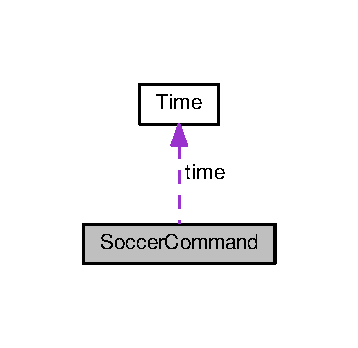
\includegraphics[width=172pt]{classSoccerCommand__coll__graph}
\end{center}
\end{figure}
\subsection*{Public Member Functions}
\begin{DoxyCompactItemize}
\item 
\hyperlink{classSoccerCommand_a504b9e27516b21fbd1e1381bd3f8b7b7}{Soccer\+Command} (\hyperlink{SoccerTypes_8h_ac986daf8a835e88572b79bcb63f5bbd5}{CommandT} com=\hyperlink{SoccerTypes_8h_ac986daf8a835e88572b79bcb63f5bbd5a38bf205bc1abc83eb30942d4e6511783}{C\+M\+D\+\_\+\+I\+L\+L\+E\+G\+AL}, double d1=\hyperlink{SoccerTypes_8h_ab232b103c74e1770db1120be5bae9be5}{Unknown\+Double\+Value}, double d2=\hyperlink{SoccerTypes_8h_ab232b103c74e1770db1120be5bae9be5}{Unknown\+Double\+Value}, double d3=\hyperlink{SoccerTypes_8h_ab232b103c74e1770db1120be5bae9be5}{Unknown\+Double\+Value})
\item 
\hyperlink{classSoccerCommand_a707aa0d64e79fbb92fa2a7c8980b5f38}{Soccer\+Command} (\hyperlink{SoccerTypes_8h_ac986daf8a835e88572b79bcb63f5bbd5}{CommandT} com, char $\ast$msg)
\item 
void \hyperlink{classSoccerCommand_a9325ca15907c55269c960cdabe8c7f7c}{make\+Command} (\hyperlink{SoccerTypes_8h_ac986daf8a835e88572b79bcb63f5bbd5}{CommandT} com, double d1=\hyperlink{SoccerTypes_8h_ab232b103c74e1770db1120be5bae9be5}{Unknown\+Double\+Value}, double d2=\hyperlink{SoccerTypes_8h_ab232b103c74e1770db1120be5bae9be5}{Unknown\+Double\+Value}, double d3=\hyperlink{SoccerTypes_8h_ab232b103c74e1770db1120be5bae9be5}{Unknown\+Double\+Value})
\item 
void \hyperlink{classSoccerCommand_a5824c426061b3270a803c3f8a38e4612}{make\+Command} (\hyperlink{SoccerTypes_8h_ac986daf8a835e88572b79bcb63f5bbd5}{CommandT} com, \hyperlink{SoccerTypes_8h_ade95094b8e117801bea82ec390cccf64}{View\+AngleT} v, \hyperlink{SoccerTypes_8h_a5ae52e4e8062de90b118eacb03e99906}{View\+QualityT} q)
\item 
void \hyperlink{classSoccerCommand_a99f3fbfbbe55135adf39c7e2e0ab356f}{make\+Command} (\hyperlink{SoccerTypes_8h_ac986daf8a835e88572b79bcb63f5bbd5}{CommandT} com, char $\ast$msg)
\item 
bool \hyperlink{classSoccerCommand_a48545e47ee0e4fd522e14862fa11e9eb}{is\+Illegal} ()
\item 
void \hyperlink{classSoccerCommand_afbd461eec23646e8af1a191e1d320071}{show} (ostream \&os)
\item 
bool \hyperlink{classSoccerCommand_a6db8db66d235145ddb4fad738b7d5600}{get\+Command\+String} (char $\ast$\hyperlink{classSoccerCommand_a0bdfba0e05fdd6a179c6ebeb5bd5c954}{str}, \hyperlink{classServerSettings}{Server\+Settings} $\ast$ss)
\end{DoxyCompactItemize}
\subsection*{Public Attributes}
\begin{DoxyCompactItemize}
\item 
\hyperlink{classTime}{Time} \hyperlink{classSoccerCommand_a5ce253af032683290460f177259912a6}{time}
\item 
\hyperlink{SoccerTypes_8h_ac986daf8a835e88572b79bcb63f5bbd5}{CommandT} \hyperlink{classSoccerCommand_a2e7d259965a11bacdc5eaba92e07dd24}{command\+Type}
\item 
double \hyperlink{classSoccerCommand_ac7c92357a850fcb7c0fba88c4867cbc1}{d\+Angle}
\item 
double \hyperlink{classSoccerCommand_aed60b006f38743bdd3c07e859b63f373}{d\+Power}
\item 
\hyperlink{SoccerTypes_8h_a5ae52e4e8062de90b118eacb03e99906}{View\+QualityT} \hyperlink{classSoccerCommand_a57d448f80f64ada2ca96506877bfc8b0}{vq}
\item 
\hyperlink{SoccerTypes_8h_ade95094b8e117801bea82ec390cccf64}{View\+AngleT} \hyperlink{classSoccerCommand_aa8709a9f44ea2feecd89dddf966dcb9e}{va}
\item 
double \hyperlink{classSoccerCommand_a91dc3c7136ee949d769371593cd1c280}{dX}
\item 
double \hyperlink{classSoccerCommand_acf593fd8e092f9352a0367f9aa5e1a40}{dY}
\item 
char \hyperlink{classSoccerCommand_a0bdfba0e05fdd6a179c6ebeb5bd5c954}{str} \mbox{[}\hyperlink{SoccerTypes_8h_a6ec2194d8f75b7a31ebe340c144165a2}{M\+A\+X\+\_\+\+S\+A\+Y\+\_\+\+M\+SG}\mbox{]}
\item 
int \hyperlink{classSoccerCommand_aa675c370ba898ae373c0e45f400f3137}{i\+Times}
\end{DoxyCompactItemize}


\subsection{Detailed Description}
This class resembles a \hyperlink{classSoccerCommand}{Soccer\+Command} that contains all the information about a command that can be sent to the server, but the format is independent from the server implementation. A \hyperlink{classSoccerCommand}{Soccer\+Command} can be created and before it is sent to the server, be converted to the actual string representation understood by the server. 

\subsection{Constructor \& Destructor Documentation}
\index{Soccer\+Command@{Soccer\+Command}!Soccer\+Command@{Soccer\+Command}}
\index{Soccer\+Command@{Soccer\+Command}!Soccer\+Command@{Soccer\+Command}}
\subsubsection[{\texorpdfstring{Soccer\+Command(\+Command\+T com=\+C\+M\+D\+\_\+\+I\+L\+L\+E\+G\+A\+L, double d1=\+Unknown\+Double\+Value, double d2=\+Unknown\+Double\+Value, double d3=\+Unknown\+Double\+Value)}{SoccerCommand(CommandT com=CMD_ILLEGAL, double d1=UnknownDoubleValue, double d2=UnknownDoubleValue, double d3=UnknownDoubleValue)}}]{\setlength{\rightskip}{0pt plus 5cm}Soccer\+Command\+::\+Soccer\+Command (
\begin{DoxyParamCaption}
\item[{{\bf CommandT}}]{com = {\ttfamily {\bf C\+M\+D\+\_\+\+I\+L\+L\+E\+G\+AL}}, }
\item[{double}]{d1 = {\ttfamily {\bf Unknown\+Double\+Value}}, }
\item[{double}]{d2 = {\ttfamily {\bf Unknown\+Double\+Value}}, }
\item[{double}]{d3 = {\ttfamily {\bf Unknown\+Double\+Value}}}
\end{DoxyParamCaption}
)}\hypertarget{classSoccerCommand_a504b9e27516b21fbd1e1381bd3f8b7b7}{}\label{classSoccerCommand_a504b9e27516b21fbd1e1381bd3f8b7b7}
This is a constructor for the \hyperlink{classSoccerCommand}{Soccer\+Command} class. It creates a command using the passed arguments (with all default illegal values). Depending on the specified CommandT the parameters are used in different ways. See the method make\+Command for an explanation of these values. 
\begin{DoxyParams}{Parameters}
{\em com} & command\+Type for this \hyperlink{classSoccerCommand}{Soccer\+Command} \\
\hline
{\em d1} & 1st argument, meaning depends on com (default Unknown\+Double\+Value) \\
\hline
{\em d2} & 2nd argument, meaning depends on com (default Unknown\+Double\+Value) \\
\hline
{\em d3} & 3rd argument, meaning depends on com (default Unknown\+Double\+Value) \\
\hline
\end{DoxyParams}
\begin{DoxyReturn}{Returns}
\hyperlink{classSoccerCommand}{Soccer\+Command} with the specified parameters. 
\end{DoxyReturn}
\index{Soccer\+Command@{Soccer\+Command}!Soccer\+Command@{Soccer\+Command}}
\index{Soccer\+Command@{Soccer\+Command}!Soccer\+Command@{Soccer\+Command}}
\subsubsection[{\texorpdfstring{Soccer\+Command(\+Command\+T com, char $\ast$msg)}{SoccerCommand(CommandT com, char *msg)}}]{\setlength{\rightskip}{0pt plus 5cm}Soccer\+Command\+::\+Soccer\+Command (
\begin{DoxyParamCaption}
\item[{{\bf CommandT}}]{com, }
\item[{char $\ast$}]{msg}
\end{DoxyParamCaption}
)}\hypertarget{classSoccerCommand_a707aa0d64e79fbb92fa2a7c8980b5f38}{}\label{classSoccerCommand_a707aa0d64e79fbb92fa2a7c8980b5f38}
This is a constructor for the \hyperlink{classSoccerCommand}{Soccer\+Command} when the command\+Type is a say message. 
\begin{DoxyParams}{Parameters}
{\em com} & command\+Type for this \hyperlink{classSoccerCommand}{Soccer\+Command} (must be C\+M\+D\+\_\+\+S\+AY). \\
\hline
{\em msg} & message for this \hyperlink{classSoccerCommand}{Soccer\+Command} \\
\hline
\end{DoxyParams}


\subsection{Member Function Documentation}
\index{Soccer\+Command@{Soccer\+Command}!get\+Command\+String@{get\+Command\+String}}
\index{get\+Command\+String@{get\+Command\+String}!Soccer\+Command@{Soccer\+Command}}
\subsubsection[{\texorpdfstring{get\+Command\+String(char $\ast$str, Server\+Settings $\ast$ss)}{getCommandString(char *str, ServerSettings *ss)}}]{\setlength{\rightskip}{0pt plus 5cm}bool Soccer\+Command\+::get\+Command\+String (
\begin{DoxyParamCaption}
\item[{char $\ast$}]{str, }
\item[{{\bf Server\+Settings} $\ast$}]{ss}
\end{DoxyParamCaption}
)}\hypertarget{classSoccerCommand_a6db8db66d235145ddb4fad738b7d5600}{}\label{classSoccerCommand_a6db8db66d235145ddb4fad738b7d5600}
This method returns a command string that is understood by the server from a \hyperlink{classSoccerCommand}{Soccer\+Command}. The resulting string is put in the second argument and returned by the method. A reference to \hyperlink{classServerSettings}{Server\+Settings} is passed as the second argument to check whether the values in the \hyperlink{classSoccerCommand}{Soccer\+Command} are legal.


\begin{DoxyParams}{Parameters}
{\em str} & resulting string (enough space for M\+A\+X\+\_\+\+M\+SG should be allocated) \\
\hline
{\em ss} & reference to serversettings class. \\
\hline
\end{DoxyParams}
\begin{DoxyReturn}{Returns}
resulting boolean indicating whether error occurred or not 
\end{DoxyReturn}
\index{Soccer\+Command@{Soccer\+Command}!is\+Illegal@{is\+Illegal}}
\index{is\+Illegal@{is\+Illegal}!Soccer\+Command@{Soccer\+Command}}
\subsubsection[{\texorpdfstring{is\+Illegal()}{isIllegal()}}]{\setlength{\rightskip}{0pt plus 5cm}bool Soccer\+Command\+::is\+Illegal (
\begin{DoxyParamCaption}
{}
\end{DoxyParamCaption}
)}\hypertarget{classSoccerCommand_a48545e47ee0e4fd522e14862fa11e9eb}{}\label{classSoccerCommand_a48545e47ee0e4fd522e14862fa11e9eb}
This method returns whether this \hyperlink{classSoccerCommand}{Soccer\+Command} is illegal, that is the \hyperlink{classSoccerCommand}{Soccer\+Command} hasn\textquotesingle{}t been filled yet. This means that no command would be performed when this command is sent to the server. \begin{DoxyReturn}{Returns}
bool indicating whether the current Command is illegal 
\end{DoxyReturn}
\index{Soccer\+Command@{Soccer\+Command}!make\+Command@{make\+Command}}
\index{make\+Command@{make\+Command}!Soccer\+Command@{Soccer\+Command}}
\subsubsection[{\texorpdfstring{make\+Command(\+Command\+T com, double d1=\+Unknown\+Double\+Value, double d2=\+Unknown\+Double\+Value, double d3=\+Unknown\+Double\+Value)}{makeCommand(CommandT com, double d1=UnknownDoubleValue, double d2=UnknownDoubleValue, double d3=UnknownDoubleValue)}}]{\setlength{\rightskip}{0pt plus 5cm}void Soccer\+Command\+::make\+Command (
\begin{DoxyParamCaption}
\item[{{\bf CommandT}}]{com, }
\item[{double}]{d1 = {\ttfamily {\bf Unknown\+Double\+Value}}, }
\item[{double}]{d2 = {\ttfamily {\bf Unknown\+Double\+Value}}, }
\item[{double}]{d3 = {\ttfamily {\bf Unknown\+Double\+Value}}}
\end{DoxyParamCaption}
)}\hypertarget{classSoccerCommand_a9325ca15907c55269c960cdabe8c7f7c}{}\label{classSoccerCommand_a9325ca15907c55269c960cdabe8c7f7c}
This method create a \hyperlink{classSoccerCommand}{Soccer\+Command} from the specified command type and the parameters. The parameters have a different meaning depending on the given command type. Not all command types are listed, since the other command types need different parameters. So see the other overloaded methods for that.
\begin{DoxyItemize}
\item C\+M\+D\+\_\+\+D\+A\+SH\+: d1 = power for dashing, d2 = angle for dashing
\item C\+M\+D\+\_\+\+T\+U\+RN\+: d1 = angle body is turned
\item C\+M\+D\+\_\+\+T\+U\+R\+N\+N\+E\+CK d1 = angle neck is turned
\item C\+M\+D\+\_\+\+K\+I\+CK d1 = power for kick command, d2 = angle for kick
\item C\+M\+D\+\_\+\+M\+O\+VE d1 = x position, d2 = y position, d3 = body\+\_\+angle
\item C\+M\+D\+\_\+\+C\+A\+T\+CH d1 = catch angle
\item C\+M\+D\+\_\+\+C\+H\+A\+N\+G\+E\+P\+L\+A\+Y\+ER d1 = player number, d2 = nr of new player type
\item C\+M\+D\+\_\+\+A\+T\+T\+E\+N\+T\+I\+O\+N\+TO d1 = which team, d2 = player number
\item C\+M\+D\+\_\+\+T\+A\+C\+K\+LE d1 = power of the tackle 
\begin{DoxyParams}{Parameters}
{\em com} & command type specifying the kind of command \\
\hline
{\em d1} & meaning depends on the specified command type (see above) \\
\hline
{\em d2} & meaning depends on the specified command type (see above) \\
\hline
{\em d3} & meaning depends on the specified command type (see above) \\
\hline
\end{DoxyParams}

\end{DoxyItemize}\index{Soccer\+Command@{Soccer\+Command}!make\+Command@{make\+Command}}
\index{make\+Command@{make\+Command}!Soccer\+Command@{Soccer\+Command}}
\subsubsection[{\texorpdfstring{make\+Command(\+Command\+T com, View\+Angle\+T v, View\+Quality\+T q)}{makeCommand(CommandT com, ViewAngleT v, ViewQualityT q)}}]{\setlength{\rightskip}{0pt plus 5cm}void Soccer\+Command\+::make\+Command (
\begin{DoxyParamCaption}
\item[{{\bf CommandT}}]{com, }
\item[{{\bf View\+AngleT}}]{v, }
\item[{{\bf View\+QualityT}}]{q}
\end{DoxyParamCaption}
)}\hypertarget{classSoccerCommand_a5824c426061b3270a803c3f8a38e4612}{}\label{classSoccerCommand_a5824c426061b3270a803c3f8a38e4612}
This method creates a \hyperlink{classSoccerCommand}{Soccer\+Command} for the command type C\+M\+D\+\_\+\+C\+H\+A\+N\+G\+E\+V\+I\+EW. 
\begin{DoxyParams}{Parameters}
{\em com} & command type specifying the kind of command \\
\hline
{\em v} & view angle for the change view command \\
\hline
{\em q} & view quality for the change view command \\
\hline
\end{DoxyParams}
\index{Soccer\+Command@{Soccer\+Command}!make\+Command@{make\+Command}}
\index{make\+Command@{make\+Command}!Soccer\+Command@{Soccer\+Command}}
\subsubsection[{\texorpdfstring{make\+Command(\+Command\+T com, char $\ast$msg)}{makeCommand(CommandT com, char *msg)}}]{\setlength{\rightskip}{0pt plus 5cm}void Soccer\+Command\+::make\+Command (
\begin{DoxyParamCaption}
\item[{{\bf CommandT}}]{com, }
\item[{char $\ast$}]{msg}
\end{DoxyParamCaption}
)}\hypertarget{classSoccerCommand_a99f3fbfbbe55135adf39c7e2e0ab356f}{}\label{classSoccerCommand_a99f3fbfbbe55135adf39c7e2e0ab356f}
This method creates a command for the command type C\+M\+D\+\_\+\+S\+AY that accepts a string as parameter. 
\begin{DoxyParams}{Parameters}
{\em com} & command type specifying the kind of command. \\
\hline
{\em msg} & string message that is added to the say message. \\
\hline
\end{DoxyParams}
\index{Soccer\+Command@{Soccer\+Command}!show@{show}}
\index{show@{show}!Soccer\+Command@{Soccer\+Command}}
\subsubsection[{\texorpdfstring{show(ostream \&os)}{show(ostream &os)}}]{\setlength{\rightskip}{0pt plus 5cm}void Soccer\+Command\+::show (
\begin{DoxyParamCaption}
\item[{ostream \&}]{os}
\end{DoxyParamCaption}
)}\hypertarget{classSoccerCommand_afbd461eec23646e8af1a191e1d320071}{}\label{classSoccerCommand_afbd461eec23646e8af1a191e1d320071}
This method prints the current command to the specified output stream. 
\begin{DoxyParams}{Parameters}
{\em os} & output stream to which information is printed. \\
\hline
\end{DoxyParams}


\subsection{Member Data Documentation}
\index{Soccer\+Command@{Soccer\+Command}!command\+Type@{command\+Type}}
\index{command\+Type@{command\+Type}!Soccer\+Command@{Soccer\+Command}}
\subsubsection[{\texorpdfstring{command\+Type}{commandType}}]{\setlength{\rightskip}{0pt plus 5cm}{\bf CommandT} Soccer\+Command\+::command\+Type}\hypertarget{classSoccerCommand_a2e7d259965a11bacdc5eaba92e07dd24}{}\label{classSoccerCommand_a2e7d259965a11bacdc5eaba92e07dd24}
type of this command \index{Soccer\+Command@{Soccer\+Command}!d\+Angle@{d\+Angle}}
\index{d\+Angle@{d\+Angle}!Soccer\+Command@{Soccer\+Command}}
\subsubsection[{\texorpdfstring{d\+Angle}{dAngle}}]{\setlength{\rightskip}{0pt plus 5cm}double Soccer\+Command\+::d\+Angle}\hypertarget{classSoccerCommand_ac7c92357a850fcb7c0fba88c4867cbc1}{}\label{classSoccerCommand_ac7c92357a850fcb7c0fba88c4867cbc1}
angle of this command (for turn,turn\+\_\+neck and dash) \index{Soccer\+Command@{Soccer\+Command}!d\+Power@{d\+Power}}
\index{d\+Power@{d\+Power}!Soccer\+Command@{Soccer\+Command}}
\subsubsection[{\texorpdfstring{d\+Power}{dPower}}]{\setlength{\rightskip}{0pt plus 5cm}double Soccer\+Command\+::d\+Power}\hypertarget{classSoccerCommand_aed60b006f38743bdd3c07e859b63f373}{}\label{classSoccerCommand_aed60b006f38743bdd3c07e859b63f373}
power of this command (for kick,dash) \index{Soccer\+Command@{Soccer\+Command}!dX@{dX}}
\index{dX@{dX}!Soccer\+Command@{Soccer\+Command}}
\subsubsection[{\texorpdfstring{dX}{dX}}]{\setlength{\rightskip}{0pt plus 5cm}double Soccer\+Command\+::dX}\hypertarget{classSoccerCommand_a91dc3c7136ee949d769371593cd1c280}{}\label{classSoccerCommand_a91dc3c7136ee949d769371593cd1c280}
x coordinate (for move) \index{Soccer\+Command@{Soccer\+Command}!dY@{dY}}
\index{dY@{dY}!Soccer\+Command@{Soccer\+Command}}
\subsubsection[{\texorpdfstring{dY}{dY}}]{\setlength{\rightskip}{0pt plus 5cm}double Soccer\+Command\+::dY}\hypertarget{classSoccerCommand_acf593fd8e092f9352a0367f9aa5e1a40}{}\label{classSoccerCommand_acf593fd8e092f9352a0367f9aa5e1a40}
y coordinate (for move) \index{Soccer\+Command@{Soccer\+Command}!i\+Times@{i\+Times}}
\index{i\+Times@{i\+Times}!Soccer\+Command@{Soccer\+Command}}
\subsubsection[{\texorpdfstring{i\+Times}{iTimes}}]{\setlength{\rightskip}{0pt plus 5cm}int Soccer\+Command\+::i\+Times}\hypertarget{classSoccerCommand_aa675c370ba898ae373c0e45f400f3137}{}\label{classSoccerCommand_aa675c370ba898ae373c0e45f400f3137}
how many cycles will a command be sent \index{Soccer\+Command@{Soccer\+Command}!str@{str}}
\index{str@{str}!Soccer\+Command@{Soccer\+Command}}
\subsubsection[{\texorpdfstring{str}{str}}]{\setlength{\rightskip}{0pt plus 5cm}char Soccer\+Command\+::str\mbox{[}{\bf M\+A\+X\+\_\+\+S\+A\+Y\+\_\+\+M\+SG}\mbox{]}}\hypertarget{classSoccerCommand_a0bdfba0e05fdd6a179c6ebeb5bd5c954}{}\label{classSoccerCommand_a0bdfba0e05fdd6a179c6ebeb5bd5c954}
str (for say) \index{Soccer\+Command@{Soccer\+Command}!time@{time}}
\index{time@{time}!Soccer\+Command@{Soccer\+Command}}
\subsubsection[{\texorpdfstring{time}{time}}]{\setlength{\rightskip}{0pt plus 5cm}{\bf Time} Soccer\+Command\+::time}\hypertarget{classSoccerCommand_a5ce253af032683290460f177259912a6}{}\label{classSoccerCommand_a5ce253af032683290460f177259912a6}
command time, will be set by worldmodel \index{Soccer\+Command@{Soccer\+Command}!va@{va}}
\index{va@{va}!Soccer\+Command@{Soccer\+Command}}
\subsubsection[{\texorpdfstring{va}{va}}]{\setlength{\rightskip}{0pt plus 5cm}{\bf View\+AngleT} Soccer\+Command\+::va}\hypertarget{classSoccerCommand_aa8709a9f44ea2feecd89dddf966dcb9e}{}\label{classSoccerCommand_aa8709a9f44ea2feecd89dddf966dcb9e}
view angle (for change\+\_\+view) \index{Soccer\+Command@{Soccer\+Command}!vq@{vq}}
\index{vq@{vq}!Soccer\+Command@{Soccer\+Command}}
\subsubsection[{\texorpdfstring{vq}{vq}}]{\setlength{\rightskip}{0pt plus 5cm}{\bf View\+QualityT} Soccer\+Command\+::vq}\hypertarget{classSoccerCommand_a57d448f80f64ada2ca96506877bfc8b0}{}\label{classSoccerCommand_a57d448f80f64ada2ca96506877bfc8b0}
view quality (for change\+\_\+view) 

The documentation for this class was generated from the following files\+:\begin{DoxyCompactItemize}
\item 
src/\hyperlink{SoccerTypes_8h}{Soccer\+Types.\+h}\item 
src/\hyperlink{SoccerTypes_8cpp}{Soccer\+Types.\+cpp}\end{DoxyCompactItemize}

\hypertarget{classSoccerTypes}{}\section{Soccer\+Types Class Reference}
\label{classSoccerTypes}\index{Soccer\+Types@{Soccer\+Types}}


{\ttfamily \#include $<$Soccer\+Types.\+h$>$}

\subsection*{Static Public Member Functions}
\begin{DoxyCompactItemize}
\item 
static char $\ast$ \hyperlink{classSoccerTypes_a5f32d677c6400f8b19b3edb19fa32283}{get\+Object\+Str} (char $\ast$str\+Buf, \hyperlink{SoccerTypes_8h_ad4b701fa66e7d26c054ed15b7820c77c}{ObjectT} o, const char $\ast$str\+Te=N\+U\+LL)
\item 
static \hyperlink{SoccerTypes_8h_ad4b701fa66e7d26c054ed15b7820c77c}{ObjectT} \hyperlink{classSoccerTypes_a6bd31e435a9d55a8654adc8630a2484a}{get\+Object\+From\+Str} (char $\ast$$\ast$str, bool $\ast$\hyperlink{classSoccerTypes_a35b0354996d20c68c047162d14359f24}{is\+Goalie}, const char $\ast$str\+Team)
\item 
static bool \hyperlink{classSoccerTypes_addc22247cfbaacd256e68b16427de975}{is\+In\+Set} (\hyperlink{SoccerTypes_8h_ad4b701fa66e7d26c054ed15b7820c77c}{ObjectT} o, \hyperlink{SoccerTypes_8h_a30481b85f5315bc8f0d7a9e0468ea81f}{Object\+SetT} o\+\_\+s, \hyperlink{SoccerTypes_8h_ad4b701fa66e7d26c054ed15b7820c77c}{ObjectT} object\+Goalie=\hyperlink{SoccerTypes_8h_ad4b701fa66e7d26c054ed15b7820c77ca4256d12157ba1b277fcd6c5b1ada9d08}{O\+B\+J\+E\+C\+T\+\_\+\+T\+E\+A\+M\+M\+A\+T\+E\+\_\+1})
\item 
static bool \hyperlink{classSoccerTypes_ad47af414002fdfff182f2d9c8ec877f1}{is\+Player\+Type\+In\+Set} (\hyperlink{SoccerTypes_8h_a88daf580b042467ccd4098107cffc718}{PlayerT} p, \hyperlink{SoccerTypes_8h_afbb545db37d2371bdcf6936de7504d00}{Player\+SetT} p\+\_\+s)
\item 
static bool \hyperlink{classSoccerTypes_a5d3e343c52d9d2fd3d7d3c8ad7c698c9}{is\+Flag} (\hyperlink{SoccerTypes_8h_ad4b701fa66e7d26c054ed15b7820c77c}{ObjectT} o)
\item 
static bool \hyperlink{classSoccerTypes_af50cc869d335bbd3b7409b25fe5c937a}{is\+Line} (\hyperlink{SoccerTypes_8h_ad4b701fa66e7d26c054ed15b7820c77c}{ObjectT} o)
\item 
static bool \hyperlink{classSoccerTypes_aedb013f6f28627bfcd967df008045874}{is\+Goal} (\hyperlink{SoccerTypes_8h_ad4b701fa66e7d26c054ed15b7820c77c}{ObjectT} o)
\item 
static \hyperlink{SoccerTypes_8h_ad4b701fa66e7d26c054ed15b7820c77c}{ObjectT} \hyperlink{classSoccerTypes_adba75e01e97f08cd24421e3a84f58add}{get\+Own\+Goal} (\hyperlink{SoccerTypes_8h_a8e9b8119c00121a197203aca01d5b090}{SideT} s)
\item 
static \hyperlink{SoccerTypes_8h_ad4b701fa66e7d26c054ed15b7820c77c}{ObjectT} \hyperlink{classSoccerTypes_a607e44094be87badb3c55ab2e920e0bc}{get\+Goal\+Opponent} (\hyperlink{SoccerTypes_8h_a8e9b8119c00121a197203aca01d5b090}{SideT} s)
\item 
static bool \hyperlink{classSoccerTypes_a2451e7b0cec7daa0fdfd2867967e1fd1}{is\+Ball} (\hyperlink{SoccerTypes_8h_ad4b701fa66e7d26c054ed15b7820c77c}{ObjectT} o)
\item 
static bool \hyperlink{classSoccerTypes_ae712af370baa2f7fdcb0916d6ab59d29}{is\+Teammate} (\hyperlink{SoccerTypes_8h_ad4b701fa66e7d26c054ed15b7820c77c}{ObjectT} o)
\item 
static bool \hyperlink{classSoccerTypes_aeda4e30db06751a19832b2ceba20ede5}{is\+Opponent} (\hyperlink{SoccerTypes_8h_ad4b701fa66e7d26c054ed15b7820c77c}{ObjectT} o)
\item 
static bool \hyperlink{classSoccerTypes_a35b0354996d20c68c047162d14359f24}{is\+Goalie} (\hyperlink{SoccerTypes_8h_ad4b701fa66e7d26c054ed15b7820c77c}{ObjectT} o)
\item 
static bool \hyperlink{classSoccerTypes_a7a8b2cadc840bb68e33d68be12b07021}{is\+Player} (\hyperlink{SoccerTypes_8h_ad4b701fa66e7d26c054ed15b7820c77c}{ObjectT} o)
\item 
static bool \hyperlink{classSoccerTypes_a64d7793f1d82a653ddb1d3ac710e3b5a}{is\+Known\+Player} (\hyperlink{SoccerTypes_8h_ad4b701fa66e7d26c054ed15b7820c77c}{ObjectT} o)
\item 
static int \hyperlink{classSoccerTypes_ac5b6caa8a907df9c60367815eac2de44}{get\+Index} (\hyperlink{SoccerTypes_8h_ad4b701fa66e7d26c054ed15b7820c77c}{ObjectT} o)
\item 
static \hyperlink{SoccerTypes_8h_ad4b701fa66e7d26c054ed15b7820c77c}{ObjectT} \hyperlink{classSoccerTypes_a522841af2b3256f24870c2937d5f08cb}{get\+Teammate\+Object\+From\+Index} (int i\+Index)
\item 
static \hyperlink{SoccerTypes_8h_ad4b701fa66e7d26c054ed15b7820c77c}{ObjectT} \hyperlink{classSoccerTypes_a337d1985e07aec6f1ed07635c0f4f157}{get\+Opponent\+Object\+From\+Index} (int i\+Index)
\item 
static \hyperlink{classVecPosition}{Vec\+Position} \hyperlink{classSoccerTypes_ae807c95a96e03c94bc72b8dfb9d925ca}{get\+Global\+Position\+Flag} (\hyperlink{SoccerTypes_8h_ad4b701fa66e7d26c054ed15b7820c77c}{ObjectT} o, \hyperlink{SoccerTypes_8h_a8e9b8119c00121a197203aca01d5b090}{SideT} s, double d\+Goal\+Width=14.\+02)
\item 
static \hyperlink{Geometry_8h_a6bfe02ae9bb185092902092561ab2865}{Ang\+Deg} \hyperlink{classSoccerTypes_a06cd3ff3d711f5973dd6cb346a10c5ef}{get\+Global\+Angle\+Line} (\hyperlink{SoccerTypes_8h_ad4b701fa66e7d26c054ed15b7820c77c}{ObjectT} o, \hyperlink{SoccerTypes_8h_a8e9b8119c00121a197203aca01d5b090}{SideT} s)
\item 
static \hyperlink{SoccerTypes_8h_a471f1cfaf71f78e444ff420bb6646815}{Play\+ModeT} \hyperlink{classSoccerTypes_aa36ce5ecff3ba4298ab09dab817a1a3a}{get\+Play\+Mode\+From\+Str} (char $\ast$str)
\item 
static \hyperlink{SoccerTypes_8h_a471f1cfaf71f78e444ff420bb6646815}{Play\+ModeT} \hyperlink{classSoccerTypes_a6aaf3a7d2f3095ce339ace6e431e9dd4}{get\+Play\+Mode\+From\+Referee\+Message} (\hyperlink{SoccerTypes_8h_abb5fa6e95f3a11e041200e983b2c2e4c}{Referee\+MessageT} rm)
\item 
static const char $\ast$ \hyperlink{classSoccerTypes_af7d37af26b013107a1067754e56b879c}{get\+Play\+Mode\+Str} (\hyperlink{SoccerTypes_8h_a471f1cfaf71f78e444ff420bb6646815}{Play\+ModeT} p)
\item 
static const char $\ast$ \hyperlink{classSoccerTypes_a417b8d47a0b9cd1d5f2f600d87e003d4}{get\+Referee\+Message\+Str} (\hyperlink{SoccerTypes_8h_abb5fa6e95f3a11e041200e983b2c2e4c}{Referee\+MessageT} r)
\item 
static \hyperlink{SoccerTypes_8h_abb5fa6e95f3a11e041200e983b2c2e4c}{Referee\+MessageT} \hyperlink{classSoccerTypes_a5d9c0abf0d9a0a0a3467271b11213b5d}{get\+Referee\+Message\+From\+Str} (char $\ast$str)
\item 
static const char $\ast$ \hyperlink{classSoccerTypes_a9c90b74496a950dc11008a24a2b4471b}{get\+View\+Angle\+Str} (\hyperlink{SoccerTypes_8h_ade95094b8e117801bea82ec390cccf64}{View\+AngleT} v)
\item 
static \hyperlink{SoccerTypes_8h_ade95094b8e117801bea82ec390cccf64}{View\+AngleT} \hyperlink{classSoccerTypes_a279fd0046e772250c94b3de03c9cf07c}{get\+View\+Angle\+From\+Str} (char $\ast$str)
\item 
static \hyperlink{Geometry_8h_a6bfe02ae9bb185092902092561ab2865}{Ang\+Deg} \hyperlink{classSoccerTypes_a75a2e4f0e8a9d13e79049d16e0334789}{get\+Half\+View\+Angle\+Value} (\hyperlink{SoccerTypes_8h_ade95094b8e117801bea82ec390cccf64}{View\+AngleT} va)
\item 
static const char $\ast$ \hyperlink{classSoccerTypes_a9fdc4594b395c2fca8299f5d27a1be2e}{get\+View\+Quality\+Str} (\hyperlink{SoccerTypes_8h_a5ae52e4e8062de90b118eacb03e99906}{View\+QualityT} v)
\item 
static \hyperlink{SoccerTypes_8h_a5ae52e4e8062de90b118eacb03e99906}{View\+QualityT} \hyperlink{classSoccerTypes_aa090cfc7509655fec9499b5bbe978edb}{get\+View\+Quality\+From\+Str} (char $\ast$str)
\item 
static const char $\ast$ \hyperlink{classSoccerTypes_a184bfac5cbaf2faf45077b0eae2c67e2}{get\+Command\+Str} (\hyperlink{SoccerTypes_8h_ac986daf8a835e88572b79bcb63f5bbd5}{CommandT} com)
\item 
static bool \hyperlink{classSoccerTypes_aee7fadf2b1a83daa0f5c00a1713d3b9e}{is\+Primary\+Command} (\hyperlink{SoccerTypes_8h_ac986daf8a835e88572b79bcb63f5bbd5}{CommandT} com)
\item 
static const char $\ast$ \hyperlink{classSoccerTypes_a2164196d89209e3d91f3c014d3c4affd}{get\+Side\+Str} (\hyperlink{SoccerTypes_8h_a8e9b8119c00121a197203aca01d5b090}{SideT} s)
\item 
static \hyperlink{SoccerTypes_8h_a8e9b8119c00121a197203aca01d5b090}{SideT} \hyperlink{classSoccerTypes_a9f7070f4790003b7775a6ffcd12e1352}{get\+Side\+From\+Str} (char $\ast$str)
\item 
static const char $\ast$ \hyperlink{classSoccerTypes_a0ecbebb96c02a8f7e28678458ec550e2}{get\+Ball\+Status\+Str} (\hyperlink{SoccerTypes_8h_aaeea770261a090c519643331173a327f}{Ball\+StatusT} bs)
\item 
static \hyperlink{SoccerTypes_8h_aaeea770261a090c519643331173a327f}{Ball\+StatusT} \hyperlink{classSoccerTypes_ae05c4b5a1789d3372f444b60c0f1f389}{get\+Ball\+Status\+From\+Str} (char $\ast$str)
\item 
static \hyperlink{Geometry_8h_a6bfe02ae9bb185092902092561ab2865}{Ang\+Deg} \hyperlink{classSoccerTypes_ab89399779d83b23ccf1d01d8d46f5c3b}{get\+Angle\+From\+Direction} (\hyperlink{SoccerTypes_8h_a8e832a4ec6c67d3151112ed1e1c67752}{DirectionT} dir)
\end{DoxyCompactItemize}


\subsection{Detailed Description}
The class \hyperlink{classSoccerTypes}{Soccer\+Types} contains different methods to work with the different enumerations defined in \hyperlink{SoccerTypes_8h}{Soccer\+Types.\+h}. It is possible to convert soccertypes to strings and strings to soccertypes. It is also possible to get more specific information about some of the soccertypes. All methods are static so it is possible to call the methods without instantiating the class. 

\subsection{Member Function Documentation}
\index{Soccer\+Types@{Soccer\+Types}!get\+Angle\+From\+Direction@{get\+Angle\+From\+Direction}}
\index{get\+Angle\+From\+Direction@{get\+Angle\+From\+Direction}!Soccer\+Types@{Soccer\+Types}}
\subsubsection[{\texorpdfstring{get\+Angle\+From\+Direction(\+Direction\+T dir)}{getAngleFromDirection(DirectionT dir)}}]{\setlength{\rightskip}{0pt plus 5cm}{\bf Ang\+Deg} Soccer\+Types\+::get\+Angle\+From\+Direction (
\begin{DoxyParamCaption}
\item[{{\bf DirectionT}}]{dir}
\end{DoxyParamCaption}
)\hspace{0.3cm}{\ttfamily [static]}}\hypertarget{classSoccerTypes_ab89399779d83b23ccf1d01d8d46f5c3b}{}\label{classSoccerTypes_ab89399779d83b23ccf1d01d8d46f5c3b}
This method returns the angle value corresponding to the direction \textquotesingle{}dir\textquotesingle{}. \index{Soccer\+Types@{Soccer\+Types}!get\+Ball\+Status\+From\+Str@{get\+Ball\+Status\+From\+Str}}
\index{get\+Ball\+Status\+From\+Str@{get\+Ball\+Status\+From\+Str}!Soccer\+Types@{Soccer\+Types}}
\subsubsection[{\texorpdfstring{get\+Ball\+Status\+From\+Str(char $\ast$str)}{getBallStatusFromStr(char *str)}}]{\setlength{\rightskip}{0pt plus 5cm}{\bf Ball\+StatusT} Soccer\+Types\+::get\+Ball\+Status\+From\+Str (
\begin{DoxyParamCaption}
\item[{char $\ast$}]{str}
\end{DoxyParamCaption}
)\hspace{0.3cm}{\ttfamily [static]}}\hypertarget{classSoccerTypes_ae05c4b5a1789d3372f444b60c0f1f389}{}\label{classSoccerTypes_ae05c4b5a1789d3372f444b60c0f1f389}
This method returns the Ball\+Status from the string that is passed as the first argument. 
\begin{DoxyParams}{Parameters}
{\em str} & pointer to a string that contains ball status info at index 0\\
\hline
\end{DoxyParams}
\begin{DoxyReturn}{Returns}
Ball\+Status of string representation, B\+S\+\_\+\+I\+L\+L\+E\+G\+AL if it is not known 
\end{DoxyReturn}
\index{Soccer\+Types@{Soccer\+Types}!get\+Ball\+Status\+Str@{get\+Ball\+Status\+Str}}
\index{get\+Ball\+Status\+Str@{get\+Ball\+Status\+Str}!Soccer\+Types@{Soccer\+Types}}
\subsubsection[{\texorpdfstring{get\+Ball\+Status\+Str(\+Ball\+Status\+T bs)}{getBallStatusStr(BallStatusT bs)}}]{\setlength{\rightskip}{0pt plus 5cm}const char $\ast$ Soccer\+Types\+::get\+Ball\+Status\+Str (
\begin{DoxyParamCaption}
\item[{{\bf Ball\+StatusT}}]{bs}
\end{DoxyParamCaption}
)\hspace{0.3cm}{\ttfamily [static]}}\hypertarget{classSoccerTypes_a0ecbebb96c02a8f7e28678458ec550e2}{}\label{classSoccerTypes_a0ecbebb96c02a8f7e28678458ec550e2}
This method returns the string representation of the Ball\+Status as is used in the Robocup Soccer Simulation (in\+\_\+field, goal\+\_\+left, goal\+\_\+right or out\+\_\+of\+\_\+field). 
\begin{DoxyParams}{Parameters}
{\em bs} & Ball\+Status which should be converted \\
\hline
\end{DoxyParams}
\begin{DoxyReturn}{Returns}
pointer to the string (enough memory should be allocated) 
\end{DoxyReturn}
\index{Soccer\+Types@{Soccer\+Types}!get\+Command\+Str@{get\+Command\+Str}}
\index{get\+Command\+Str@{get\+Command\+Str}!Soccer\+Types@{Soccer\+Types}}
\subsubsection[{\texorpdfstring{get\+Command\+Str(\+Command\+T com)}{getCommandStr(CommandT com)}}]{\setlength{\rightskip}{0pt plus 5cm}const char $\ast$ Soccer\+Types\+::get\+Command\+Str (
\begin{DoxyParamCaption}
\item[{{\bf CommandT}}]{com}
\end{DoxyParamCaption}
)\hspace{0.3cm}{\ttfamily [static]}}\hypertarget{classSoccerTypes_a184bfac5cbaf2faf45077b0eae2c67e2}{}\label{classSoccerTypes_a184bfac5cbaf2faf45077b0eae2c67e2}
This method returns the string representation of a CommandT as is used in the Robocup Soccer Simulation 
\begin{DoxyParams}{Parameters}
{\em com} & CommandT that should be converted \\
\hline
\end{DoxyParams}
\begin{DoxyReturn}{Returns}
pointer to the string (enough memory should be allocated) 
\end{DoxyReturn}
\index{Soccer\+Types@{Soccer\+Types}!get\+Global\+Angle\+Line@{get\+Global\+Angle\+Line}}
\index{get\+Global\+Angle\+Line@{get\+Global\+Angle\+Line}!Soccer\+Types@{Soccer\+Types}}
\subsubsection[{\texorpdfstring{get\+Global\+Angle\+Line(\+Object\+T o, Side\+T s)}{getGlobalAngleLine(ObjectT o, SideT s)}}]{\setlength{\rightskip}{0pt plus 5cm}{\bf Ang\+Deg} Soccer\+Types\+::get\+Global\+Angle\+Line (
\begin{DoxyParamCaption}
\item[{{\bf ObjectT}}]{o, }
\item[{{\bf SideT}}]{s}
\end{DoxyParamCaption}
)\hspace{0.3cm}{\ttfamily [static]}}\hypertarget{classSoccerTypes_a06cd3ff3d711f5973dd6cb346a10c5ef}{}\label{classSoccerTypes_a06cd3ff3d711f5973dd6cb346a10c5ef}
This method returns the global angle of a lines on the field. The global angle differs for the left and right side. For both teams the line behind the opponent goal is seen with global angle 0. Only for the left team this is the right line and for the right team this is the left line.


\begin{DoxyParams}{Parameters}
{\em o} & one of the four line objects \\
\hline
{\em s} & side on which the team was started \\
\hline
\end{DoxyParams}
\begin{DoxyReturn}{Returns}
Ang\+Deg global angle of this line. 
\end{DoxyReturn}
\index{Soccer\+Types@{Soccer\+Types}!get\+Global\+Position\+Flag@{get\+Global\+Position\+Flag}}
\index{get\+Global\+Position\+Flag@{get\+Global\+Position\+Flag}!Soccer\+Types@{Soccer\+Types}}
\subsubsection[{\texorpdfstring{get\+Global\+Position\+Flag(\+Object\+T o, Side\+T s, double d\+Goal\+Width=14.\+02)}{getGlobalPositionFlag(ObjectT o, SideT s, double dGoalWidth=14.02)}}]{\setlength{\rightskip}{0pt plus 5cm}{\bf Vec\+Position} Soccer\+Types\+::get\+Global\+Position\+Flag (
\begin{DoxyParamCaption}
\item[{{\bf ObjectT}}]{o, }
\item[{{\bf SideT}}]{s, }
\item[{double}]{d\+Goal\+Width = {\ttfamily 14.02}}
\end{DoxyParamCaption}
)\hspace{0.3cm}{\ttfamily [static]}}\hypertarget{classSoccerTypes_ae807c95a96e03c94bc72b8dfb9d925ca}{}\label{classSoccerTypes_ae807c95a96e03c94bc72b8dfb9d925ca}
This method returns the global position on the field of a flag (a goal is also a flag). Since the global positions for both teams differ, the side of the agent team is also needed. Note that the global positions of the flags will not change in the second half. 
\begin{DoxyParams}{Parameters}
{\em o} & flag of which global position should be determined \\
\hline
{\em s} & side of your team. \\
\hline
{\em d\+Goal\+Width} & for some flags the goal\+Width is necessary (default 14.\+02) \\
\hline
\end{DoxyParams}
\begin{DoxyReturn}{Returns}
\hyperlink{classVecPosition}{Vec\+Position} representing the global position. x and y value are both Unknown\+Double\+Value when o is not a flag or goal. 
\end{DoxyReturn}
\index{Soccer\+Types@{Soccer\+Types}!get\+Goal\+Opponent@{get\+Goal\+Opponent}}
\index{get\+Goal\+Opponent@{get\+Goal\+Opponent}!Soccer\+Types@{Soccer\+Types}}
\subsubsection[{\texorpdfstring{get\+Goal\+Opponent(\+Side\+T s)}{getGoalOpponent(SideT s)}}]{\setlength{\rightskip}{0pt plus 5cm}{\bf ObjectT} Soccer\+Types\+::get\+Goal\+Opponent (
\begin{DoxyParamCaption}
\item[{{\bf SideT}}]{s}
\end{DoxyParamCaption}
)\hspace{0.3cm}{\ttfamily [static]}}\hypertarget{classSoccerTypes_a607e44094be87badb3c55ab2e920e0bc}{}\label{classSoccerTypes_a607e44094be87badb3c55ab2e920e0bc}
This method returns the object representing the opponent goal 
\begin{DoxyParams}{Parameters}
{\em s} & own side\\
\hline
\end{DoxyParams}
\begin{DoxyReturn}{Returns}
object of the goal opponent, O\+B\+J\+E\+C\+T\+\_\+\+I\+L\+L\+E\+G\+AL when s is S\+I\+D\+E\+\_\+\+I\+L\+L\+E\+G\+AL 
\end{DoxyReturn}
\index{Soccer\+Types@{Soccer\+Types}!get\+Half\+View\+Angle\+Value@{get\+Half\+View\+Angle\+Value}}
\index{get\+Half\+View\+Angle\+Value@{get\+Half\+View\+Angle\+Value}!Soccer\+Types@{Soccer\+Types}}
\subsubsection[{\texorpdfstring{get\+Half\+View\+Angle\+Value(\+View\+Angle\+T va)}{getHalfViewAngleValue(ViewAngleT va)}}]{\setlength{\rightskip}{0pt plus 5cm}{\bf Ang\+Deg} Soccer\+Types\+::get\+Half\+View\+Angle\+Value (
\begin{DoxyParamCaption}
\item[{{\bf View\+AngleT}}]{va}
\end{DoxyParamCaption}
)\hspace{0.3cm}{\ttfamily [static]}}\hypertarget{classSoccerTypes_a75a2e4f0e8a9d13e79049d16e0334789}{}\label{classSoccerTypes_a75a2e4f0e8a9d13e79049d16e0334789}
This method returns the half angle value that belongs to the View\+Angle that is given as the first argument (V\+A\+\_\+\+N\+A\+R\+R\+OW, V\+A\+\_\+\+N\+O\+R\+M\+AL or V\+A\+\_\+\+W\+I\+DE). The half view angle is returned since this makes it easier to check whether an object lies in the view cone (the global relative angle must be smaller than the half view angle.


\begin{DoxyParams}{Parameters}
{\em va} & view angle \\
\hline
\end{DoxyParams}
\begin{DoxyReturn}{Returns}
angle denoting the half of the corresponding view angle 
\end{DoxyReturn}
\index{Soccer\+Types@{Soccer\+Types}!get\+Index@{get\+Index}}
\index{get\+Index@{get\+Index}!Soccer\+Types@{Soccer\+Types}}
\subsubsection[{\texorpdfstring{get\+Index(\+Object\+T o)}{getIndex(ObjectT o)}}]{\setlength{\rightskip}{0pt plus 5cm}int Soccer\+Types\+::get\+Index (
\begin{DoxyParamCaption}
\item[{{\bf ObjectT}}]{o}
\end{DoxyParamCaption}
)\hspace{0.3cm}{\ttfamily [static]}}\hypertarget{classSoccerTypes_ac5b6caa8a907df9c60367815eac2de44}{}\label{classSoccerTypes_ac5b6caa8a907df9c60367815eac2de44}
This method returns the index of an object relative to the first object in that set. The index is always 1 smaller than its number, so O\+B\+J\+E\+C\+T\+\_\+\+O\+P\+P\+O\+N\+E\+N\+T\+\_\+1 will become 0. This can be used for indexing an array of objects. 
\begin{DoxyParams}{Parameters}
{\em o} & ObjectT type of object of which the index has to be calculated \\
\hline
\end{DoxyParams}
\begin{DoxyReturn}{Returns}
index of object or -\/1 when o was not a correct object 
\end{DoxyReturn}
\index{Soccer\+Types@{Soccer\+Types}!get\+Object\+From\+Str@{get\+Object\+From\+Str}}
\index{get\+Object\+From\+Str@{get\+Object\+From\+Str}!Soccer\+Types@{Soccer\+Types}}
\subsubsection[{\texorpdfstring{get\+Object\+From\+Str(char $\ast$$\ast$str, bool $\ast$is\+Goalie, const char $\ast$str\+Team)}{getObjectFromStr(char **str, bool *isGoalie, const char *strTeam)}}]{\setlength{\rightskip}{0pt plus 5cm}{\bf ObjectT} Soccer\+Types\+::get\+Object\+From\+Str (
\begin{DoxyParamCaption}
\item[{char $\ast$$\ast$}]{str, }
\item[{bool $\ast$}]{is\+Goalie, }
\item[{const char $\ast$}]{str\+My\+Team\+Name}
\end{DoxyParamCaption}
)\hspace{0.3cm}{\ttfamily [static]}}\hypertarget{classSoccerTypes_a6bd31e435a9d55a8654adc8630a2484a}{}\label{classSoccerTypes_a6bd31e435a9d55a8654adc8630a2484a}
This method returns an ObjectT that corresponds to the string passed as the first argument. The string representation equals the representation used in the Soccer Server. Format is with parenthesis, so possible arguments for str are (ball), (p Team\+\_\+L 1), etc.


\begin{DoxyParams}{Parameters}
{\em str} & pointer to string containing string representation of object \\
\hline
{\em is\+Goalie} & bool representing the fact whether object is a goalie \\
\hline
{\em str\+My\+Team\+Name} & in case of player or opponent object, own teamname has to be matched, when it matches it is teammate otherwise opponent\\
\hline
\end{DoxyParams}
\begin{DoxyReturn}{Returns}
return the corresponding ObjectT, O\+B\+J\+E\+C\+T\+\_\+\+I\+L\+L\+E\+G\+AL in case of error 
\end{DoxyReturn}
\index{Soccer\+Types@{Soccer\+Types}!get\+Object\+Str@{get\+Object\+Str}}
\index{get\+Object\+Str@{get\+Object\+Str}!Soccer\+Types@{Soccer\+Types}}
\subsubsection[{\texorpdfstring{get\+Object\+Str(char $\ast$str\+Buf, Object\+T o, const char $\ast$str\+Te=\+N\+U\+L\+L)}{getObjectStr(char *strBuf, ObjectT o, const char *strTe=NULL)}}]{\setlength{\rightskip}{0pt plus 5cm}char $\ast$ Soccer\+Types\+::get\+Object\+Str (
\begin{DoxyParamCaption}
\item[{char $\ast$}]{str\+Buf, }
\item[{{\bf ObjectT}}]{o, }
\item[{const char $\ast$}]{str\+Team\+Name = {\ttfamily NULL}}
\end{DoxyParamCaption}
)\hspace{0.3cm}{\ttfamily [static]}}\hypertarget{classSoccerTypes_a5f32d677c6400f8b19b3edb19fa32283}{}\label{classSoccerTypes_a5f32d677c6400f8b19b3edb19fa32283}
This method returns the string that corresponds to a specific object. This string name is exactly the same as the (short) name of the Robo\+Cup Simulation. 
\begin{DoxyParams}{Parameters}
{\em str\+Buf} & is the string in which the string representation is stored \\
\hline
{\em o} & ObjectT that has to be converted to the string representation \\
\hline
{\em str\+Team\+Name} & teamname that should be placed in case of player object \\
\hline
\end{DoxyParams}
\begin{DoxyReturn}{Returns}
pointer to str\+Buf, which contains the string representation 
\end{DoxyReturn}
\index{Soccer\+Types@{Soccer\+Types}!get\+Opponent\+Object\+From\+Index@{get\+Opponent\+Object\+From\+Index}}
\index{get\+Opponent\+Object\+From\+Index@{get\+Opponent\+Object\+From\+Index}!Soccer\+Types@{Soccer\+Types}}
\subsubsection[{\texorpdfstring{get\+Opponent\+Object\+From\+Index(int i\+Index)}{getOpponentObjectFromIndex(int iIndex)}}]{\setlength{\rightskip}{0pt plus 5cm}{\bf ObjectT} Soccer\+Types\+::get\+Opponent\+Object\+From\+Index (
\begin{DoxyParamCaption}
\item[{int}]{i\+Index}
\end{DoxyParamCaption}
)\hspace{0.3cm}{\ttfamily [static]}}\hypertarget{classSoccerTypes_a337d1985e07aec6f1ed07635c0f4f157}{}\label{classSoccerTypes_a337d1985e07aec6f1ed07635c0f4f157}
This method returns the object type of an opponent with index i\+Index. When i\+Index equals 9 for example O\+B\+J\+E\+C\+T\+\_\+\+O\+P\+P\+O\+N\+E\+N\+T\+\_\+10 is returned. 
\begin{DoxyParams}{Parameters}
{\em i\+Index} & index of opponent range is \mbox{[}0..10\mbox{]} \\
\hline
\end{DoxyParams}
\begin{DoxyReturn}{Returns}
object type corresponding to this index 
\end{DoxyReturn}
\index{Soccer\+Types@{Soccer\+Types}!get\+Own\+Goal@{get\+Own\+Goal}}
\index{get\+Own\+Goal@{get\+Own\+Goal}!Soccer\+Types@{Soccer\+Types}}
\subsubsection[{\texorpdfstring{get\+Own\+Goal(\+Side\+T s)}{getOwnGoal(SideT s)}}]{\setlength{\rightskip}{0pt plus 5cm}{\bf ObjectT} Soccer\+Types\+::get\+Own\+Goal (
\begin{DoxyParamCaption}
\item[{{\bf SideT}}]{s}
\end{DoxyParamCaption}
)\hspace{0.3cm}{\ttfamily [static]}}\hypertarget{classSoccerTypes_adba75e01e97f08cd24421e3a84f58add}{}\label{classSoccerTypes_adba75e01e97f08cd24421e3a84f58add}
This method returns the object representing the own goal 
\begin{DoxyParams}{Parameters}
{\em s} & own side \\
\hline
\end{DoxyParams}
\begin{DoxyReturn}{Returns}
object of the own goal, O\+B\+J\+E\+C\+T\+\_\+\+I\+L\+L\+E\+G\+AL when s is S\+I\+D\+E\+\_\+\+I\+L\+L\+E\+G\+AL 
\end{DoxyReturn}
\index{Soccer\+Types@{Soccer\+Types}!get\+Play\+Mode\+From\+Referee\+Message@{get\+Play\+Mode\+From\+Referee\+Message}}
\index{get\+Play\+Mode\+From\+Referee\+Message@{get\+Play\+Mode\+From\+Referee\+Message}!Soccer\+Types@{Soccer\+Types}}
\subsubsection[{\texorpdfstring{get\+Play\+Mode\+From\+Referee\+Message(\+Referee\+Message\+T rm)}{getPlayModeFromRefereeMessage(RefereeMessageT rm)}}]{\setlength{\rightskip}{0pt plus 5cm}{\bf Play\+ModeT} Soccer\+Types\+::get\+Play\+Mode\+From\+Referee\+Message (
\begin{DoxyParamCaption}
\item[{{\bf Referee\+MessageT}}]{rm}
\end{DoxyParamCaption}
)\hspace{0.3cm}{\ttfamily [static]}}\hypertarget{classSoccerTypes_a6aaf3a7d2f3095ce339ace6e431e9dd4}{}\label{classSoccerTypes_a6aaf3a7d2f3095ce339ace6e431e9dd4}
This method returns the play mode from the referee message. 
\begin{DoxyParams}{Parameters}
{\em rm} & Referee\+Message that contains the play mode \\
\hline
\end{DoxyParams}
\begin{DoxyReturn}{Returns}
Play\+ModeT of Referee\+Message, P\+M\+\_\+\+I\+L\+L\+E\+G\+AL if it is not recognized 
\end{DoxyReturn}
\index{Soccer\+Types@{Soccer\+Types}!get\+Play\+Mode\+From\+Str@{get\+Play\+Mode\+From\+Str}}
\index{get\+Play\+Mode\+From\+Str@{get\+Play\+Mode\+From\+Str}!Soccer\+Types@{Soccer\+Types}}
\subsubsection[{\texorpdfstring{get\+Play\+Mode\+From\+Str(char $\ast$str)}{getPlayModeFromStr(char *str)}}]{\setlength{\rightskip}{0pt plus 5cm}{\bf Play\+ModeT} Soccer\+Types\+::get\+Play\+Mode\+From\+Str (
\begin{DoxyParamCaption}
\item[{char $\ast$}]{str}
\end{DoxyParamCaption}
)\hspace{0.3cm}{\ttfamily [static]}}\hypertarget{classSoccerTypes_aa36ce5ecff3ba4298ab09dab817a1a3a}{}\label{classSoccerTypes_aa36ce5ecff3ba4298ab09dab817a1a3a}
This method returns the play mode associated with a string. 
\begin{DoxyParams}{Parameters}
{\em str} & representing the play mode \\
\hline
\end{DoxyParams}
\begin{DoxyReturn}{Returns}
Play\+ModeT of string, P\+M\+\_\+\+I\+L\+L\+E\+G\+AL if it is not recognized 
\end{DoxyReturn}
\index{Soccer\+Types@{Soccer\+Types}!get\+Play\+Mode\+Str@{get\+Play\+Mode\+Str}}
\index{get\+Play\+Mode\+Str@{get\+Play\+Mode\+Str}!Soccer\+Types@{Soccer\+Types}}
\subsubsection[{\texorpdfstring{get\+Play\+Mode\+Str(\+Play\+Mode\+T p)}{getPlayModeStr(PlayModeT p)}}]{\setlength{\rightskip}{0pt plus 5cm}const char $\ast$ Soccer\+Types\+::get\+Play\+Mode\+Str (
\begin{DoxyParamCaption}
\item[{{\bf Play\+ModeT}}]{pm}
\end{DoxyParamCaption}
)\hspace{0.3cm}{\ttfamily [static]}}\hypertarget{classSoccerTypes_af7d37af26b013107a1067754e56b879c}{}\label{classSoccerTypes_af7d37af26b013107a1067754e56b879c}
This method returns the string representation of a Play\+ModeT as is used in the Robocup Soccer Simulation and also said by the referee. 
\begin{DoxyParams}{Parameters}
{\em pm} & Play\+ModeT which should be converted \\
\hline
\end{DoxyParams}
\begin{DoxyReturn}{Returns}
pointer to the string (enough memory has to be allocated) 
\end{DoxyReturn}
\index{Soccer\+Types@{Soccer\+Types}!get\+Referee\+Message\+From\+Str@{get\+Referee\+Message\+From\+Str}}
\index{get\+Referee\+Message\+From\+Str@{get\+Referee\+Message\+From\+Str}!Soccer\+Types@{Soccer\+Types}}
\subsubsection[{\texorpdfstring{get\+Referee\+Message\+From\+Str(char $\ast$str)}{getRefereeMessageFromStr(char *str)}}]{\setlength{\rightskip}{0pt plus 5cm}{\bf Referee\+MessageT} Soccer\+Types\+::get\+Referee\+Message\+From\+Str (
\begin{DoxyParamCaption}
\item[{char $\ast$}]{str}
\end{DoxyParamCaption}
)\hspace{0.3cm}{\ttfamily [static]}}\hypertarget{classSoccerTypes_a5d9c0abf0d9a0a0a3467271b11213b5d}{}\label{classSoccerTypes_a5d9c0abf0d9a0a0a3467271b11213b5d}
This method returns the referee message from the string that is passed. 
\begin{DoxyParams}{Parameters}
{\em str} & pointer to a string with the referee message starting at index 0\\
\hline
\end{DoxyParams}
\begin{DoxyReturn}{Returns}
Referee\+MessageT of string representation, R\+E\+F\+C\+\_\+\+I\+L\+L\+E\+G\+AL if it fails 
\end{DoxyReturn}
\index{Soccer\+Types@{Soccer\+Types}!get\+Referee\+Message\+Str@{get\+Referee\+Message\+Str}}
\index{get\+Referee\+Message\+Str@{get\+Referee\+Message\+Str}!Soccer\+Types@{Soccer\+Types}}
\subsubsection[{\texorpdfstring{get\+Referee\+Message\+Str(\+Referee\+Message\+T r)}{getRefereeMessageStr(RefereeMessageT r)}}]{\setlength{\rightskip}{0pt plus 5cm}const char $\ast$ Soccer\+Types\+::get\+Referee\+Message\+Str (
\begin{DoxyParamCaption}
\item[{{\bf Referee\+MessageT}}]{rm}
\end{DoxyParamCaption}
)\hspace{0.3cm}{\ttfamily [static]}}\hypertarget{classSoccerTypes_a417b8d47a0b9cd1d5f2f600d87e003d4}{}\label{classSoccerTypes_a417b8d47a0b9cd1d5f2f600d87e003d4}
This method returns the string representation of a Referee\+MessageT as is used in the Robocup Soccer Simulation and said by the referee. 
\begin{DoxyParams}{Parameters}
{\em pm} & Referee\+MessageT which should be converted \\
\hline
\end{DoxyParams}
\begin{DoxyReturn}{Returns}
pointer to the string (enough memory should be allocated) 
\end{DoxyReturn}
\index{Soccer\+Types@{Soccer\+Types}!get\+Side\+From\+Str@{get\+Side\+From\+Str}}
\index{get\+Side\+From\+Str@{get\+Side\+From\+Str}!Soccer\+Types@{Soccer\+Types}}
\subsubsection[{\texorpdfstring{get\+Side\+From\+Str(char $\ast$str)}{getSideFromStr(char *str)}}]{\setlength{\rightskip}{0pt plus 5cm}{\bf SideT} Soccer\+Types\+::get\+Side\+From\+Str (
\begin{DoxyParamCaption}
\item[{char $\ast$}]{str}
\end{DoxyParamCaption}
)\hspace{0.3cm}{\ttfamily [static]}}\hypertarget{classSoccerTypes_a9f7070f4790003b7775a6ffcd12e1352}{}\label{classSoccerTypes_a9f7070f4790003b7775a6ffcd12e1352}
This method returns the SideT from the string that is passed as the first argument. 
\begin{DoxyParams}{Parameters}
{\em str} & pointer to a string that contains side info string at index 0 \\
\hline
\end{DoxyParams}
\begin{DoxyReturn}{Returns}
SideT of string representation, S\+I\+D\+E\+\_\+\+I\+L\+L\+E\+G\+AL if it is not known 
\end{DoxyReturn}
\index{Soccer\+Types@{Soccer\+Types}!get\+Side\+Str@{get\+Side\+Str}}
\index{get\+Side\+Str@{get\+Side\+Str}!Soccer\+Types@{Soccer\+Types}}
\subsubsection[{\texorpdfstring{get\+Side\+Str(\+Side\+T s)}{getSideStr(SideT s)}}]{\setlength{\rightskip}{0pt plus 5cm}const char $\ast$ Soccer\+Types\+::get\+Side\+Str (
\begin{DoxyParamCaption}
\item[{{\bf SideT}}]{s}
\end{DoxyParamCaption}
)\hspace{0.3cm}{\ttfamily [static]}}\hypertarget{classSoccerTypes_a2164196d89209e3d91f3c014d3c4affd}{}\label{classSoccerTypes_a2164196d89209e3d91f3c014d3c4affd}
This method returns the string representation of a SideT as is used in the Robocup Soccer Simulation (r or l). 
\begin{DoxyParams}{Parameters}
{\em s} & SideT which should be converted \\
\hline
\end{DoxyParams}
\begin{DoxyReturn}{Returns}
pointer to the string 
\end{DoxyReturn}
\index{Soccer\+Types@{Soccer\+Types}!get\+Teammate\+Object\+From\+Index@{get\+Teammate\+Object\+From\+Index}}
\index{get\+Teammate\+Object\+From\+Index@{get\+Teammate\+Object\+From\+Index}!Soccer\+Types@{Soccer\+Types}}
\subsubsection[{\texorpdfstring{get\+Teammate\+Object\+From\+Index(int i\+Index)}{getTeammateObjectFromIndex(int iIndex)}}]{\setlength{\rightskip}{0pt plus 5cm}{\bf ObjectT} Soccer\+Types\+::get\+Teammate\+Object\+From\+Index (
\begin{DoxyParamCaption}
\item[{int}]{i\+Index}
\end{DoxyParamCaption}
)\hspace{0.3cm}{\ttfamily [static]}}\hypertarget{classSoccerTypes_a522841af2b3256f24870c2937d5f08cb}{}\label{classSoccerTypes_a522841af2b3256f24870c2937d5f08cb}
This method returns the object type of a teammate with index i\+Index. When i\+Index equals 3 for example O\+B\+J\+E\+C\+T\+\_\+\+T\+E\+A\+M\+M\+A\+T\+E\+\_\+4 is returned. 
\begin{DoxyParams}{Parameters}
{\em i\+Index} & index of teammate range is \mbox{[}0..10\mbox{]} \\
\hline
\end{DoxyParams}
\begin{DoxyReturn}{Returns}
object type corresponding to this index 
\end{DoxyReturn}
\index{Soccer\+Types@{Soccer\+Types}!get\+View\+Angle\+From\+Str@{get\+View\+Angle\+From\+Str}}
\index{get\+View\+Angle\+From\+Str@{get\+View\+Angle\+From\+Str}!Soccer\+Types@{Soccer\+Types}}
\subsubsection[{\texorpdfstring{get\+View\+Angle\+From\+Str(char $\ast$str)}{getViewAngleFromStr(char *str)}}]{\setlength{\rightskip}{0pt plus 5cm}{\bf View\+AngleT} Soccer\+Types\+::get\+View\+Angle\+From\+Str (
\begin{DoxyParamCaption}
\item[{char $\ast$}]{str}
\end{DoxyParamCaption}
)\hspace{0.3cm}{\ttfamily [static]}}\hypertarget{classSoccerTypes_a279fd0046e772250c94b3de03c9cf07c}{}\label{classSoccerTypes_a279fd0046e772250c94b3de03c9cf07c}
This method returns et the view angle from the specified string 
\begin{DoxyParams}{Parameters}
{\em str} & pointer to a string that contains view angle string at index 0 \\
\hline
\end{DoxyParams}
\begin{DoxyReturn}{Returns}
View\+AngleT of string, V\+A\+\_\+\+I\+L\+L\+E\+G\+AL if it is not recognized 
\end{DoxyReturn}
\index{Soccer\+Types@{Soccer\+Types}!get\+View\+Angle\+Str@{get\+View\+Angle\+Str}}
\index{get\+View\+Angle\+Str@{get\+View\+Angle\+Str}!Soccer\+Types@{Soccer\+Types}}
\subsubsection[{\texorpdfstring{get\+View\+Angle\+Str(\+View\+Angle\+T v)}{getViewAngleStr(ViewAngleT v)}}]{\setlength{\rightskip}{0pt plus 5cm}const char $\ast$ Soccer\+Types\+::get\+View\+Angle\+Str (
\begin{DoxyParamCaption}
\item[{{\bf View\+AngleT}}]{va}
\end{DoxyParamCaption}
)\hspace{0.3cm}{\ttfamily [static]}}\hypertarget{classSoccerTypes_a9c90b74496a950dc11008a24a2b4471b}{}\label{classSoccerTypes_a9c90b74496a950dc11008a24a2b4471b}
This method returns the string representation of a View\+AngleT as is used in the Robocup Soccer Simulation 
\begin{DoxyParams}{Parameters}
{\em va} & View\+AngleT which should be converted \\
\hline
\end{DoxyParams}
\begin{DoxyReturn}{Returns}
pointer to the string (enough memory should be allocatd) 
\end{DoxyReturn}
\index{Soccer\+Types@{Soccer\+Types}!get\+View\+Quality\+From\+Str@{get\+View\+Quality\+From\+Str}}
\index{get\+View\+Quality\+From\+Str@{get\+View\+Quality\+From\+Str}!Soccer\+Types@{Soccer\+Types}}
\subsubsection[{\texorpdfstring{get\+View\+Quality\+From\+Str(char $\ast$str)}{getViewQualityFromStr(char *str)}}]{\setlength{\rightskip}{0pt plus 5cm}{\bf View\+QualityT} Soccer\+Types\+::get\+View\+Quality\+From\+Str (
\begin{DoxyParamCaption}
\item[{char $\ast$}]{str}
\end{DoxyParamCaption}
)\hspace{0.3cm}{\ttfamily [static]}}\hypertarget{classSoccerTypes_aa090cfc7509655fec9499b5bbe978edb}{}\label{classSoccerTypes_aa090cfc7509655fec9499b5bbe978edb}
This method returns the view quality from the string that is passed as the first argument 
\begin{DoxyParams}{Parameters}
{\em str} & pointer to a string that contains view quality string at index 0 \\
\hline
\end{DoxyParams}
\begin{DoxyReturn}{Returns}
View\+QualityT of string, V\+Q\+\_\+\+I\+L\+L\+E\+G\+AL if it is not known 
\end{DoxyReturn}
\index{Soccer\+Types@{Soccer\+Types}!get\+View\+Quality\+Str@{get\+View\+Quality\+Str}}
\index{get\+View\+Quality\+Str@{get\+View\+Quality\+Str}!Soccer\+Types@{Soccer\+Types}}
\subsubsection[{\texorpdfstring{get\+View\+Quality\+Str(\+View\+Quality\+T v)}{getViewQualityStr(ViewQualityT v)}}]{\setlength{\rightskip}{0pt plus 5cm}const char $\ast$ Soccer\+Types\+::get\+View\+Quality\+Str (
\begin{DoxyParamCaption}
\item[{{\bf View\+QualityT}}]{vq}
\end{DoxyParamCaption}
)\hspace{0.3cm}{\ttfamily [static]}}\hypertarget{classSoccerTypes_a9fdc4594b395c2fca8299f5d27a1be2e}{}\label{classSoccerTypes_a9fdc4594b395c2fca8299f5d27a1be2e}
This method returns the string representation of a View\+QualityT as is used in the Robocup Soccer Simulation 
\begin{DoxyParams}{Parameters}
{\em vq} & View\+QualityT which should be converted \\
\hline
\end{DoxyParams}
\begin{DoxyReturn}{Returns}
pointer to the string (enough memory should be allocated) 
\end{DoxyReturn}
\index{Soccer\+Types@{Soccer\+Types}!is\+Ball@{is\+Ball}}
\index{is\+Ball@{is\+Ball}!Soccer\+Types@{Soccer\+Types}}
\subsubsection[{\texorpdfstring{is\+Ball(\+Object\+T o)}{isBall(ObjectT o)}}]{\setlength{\rightskip}{0pt plus 5cm}bool Soccer\+Types\+::is\+Ball (
\begin{DoxyParamCaption}
\item[{{\bf ObjectT}}]{o}
\end{DoxyParamCaption}
)\hspace{0.3cm}{\ttfamily [static]}}\hypertarget{classSoccerTypes_a2451e7b0cec7daa0fdfd2867967e1fd1}{}\label{classSoccerTypes_a2451e7b0cec7daa0fdfd2867967e1fd1}
This method determines whether object o is the ball 
\begin{DoxyParams}{Parameters}
{\em o} & an object type \\
\hline
\end{DoxyParams}
\begin{DoxyReturn}{Returns}
bool indicating whether o is the ball (true) or not (false) 
\end{DoxyReturn}
\index{Soccer\+Types@{Soccer\+Types}!is\+Flag@{is\+Flag}}
\index{is\+Flag@{is\+Flag}!Soccer\+Types@{Soccer\+Types}}
\subsubsection[{\texorpdfstring{is\+Flag(\+Object\+T o)}{isFlag(ObjectT o)}}]{\setlength{\rightskip}{0pt plus 5cm}bool Soccer\+Types\+::is\+Flag (
\begin{DoxyParamCaption}
\item[{{\bf ObjectT}}]{o}
\end{DoxyParamCaption}
)\hspace{0.3cm}{\ttfamily [static]}}\hypertarget{classSoccerTypes_a5d3e343c52d9d2fd3d7d3c8ad7c698c9}{}\label{classSoccerTypes_a5d3e343c52d9d2fd3d7d3c8ad7c698c9}
This method determines whether object o is a flag. 
\begin{DoxyParams}{Parameters}
{\em o} & an object type \\
\hline
\end{DoxyParams}
\begin{DoxyReturn}{Returns}
bool indicating whether o is a flag (return true) or not (false) 
\end{DoxyReturn}
\index{Soccer\+Types@{Soccer\+Types}!is\+Goal@{is\+Goal}}
\index{is\+Goal@{is\+Goal}!Soccer\+Types@{Soccer\+Types}}
\subsubsection[{\texorpdfstring{is\+Goal(\+Object\+T o)}{isGoal(ObjectT o)}}]{\setlength{\rightskip}{0pt plus 5cm}bool Soccer\+Types\+::is\+Goal (
\begin{DoxyParamCaption}
\item[{{\bf ObjectT}}]{o}
\end{DoxyParamCaption}
)\hspace{0.3cm}{\ttfamily [static]}}\hypertarget{classSoccerTypes_aedb013f6f28627bfcd967df008045874}{}\label{classSoccerTypes_aedb013f6f28627bfcd967df008045874}
This method determines whether object o is a goal 
\begin{DoxyParams}{Parameters}
{\em o} & an object type \\
\hline
\end{DoxyParams}
\begin{DoxyReturn}{Returns}
bool indicating whether o is a goal (return true) or not (false) 
\end{DoxyReturn}
\index{Soccer\+Types@{Soccer\+Types}!is\+Goalie@{is\+Goalie}}
\index{is\+Goalie@{is\+Goalie}!Soccer\+Types@{Soccer\+Types}}
\subsubsection[{\texorpdfstring{is\+Goalie(\+Object\+T o)}{isGoalie(ObjectT o)}}]{\setlength{\rightskip}{0pt plus 5cm}bool Soccer\+Types\+::is\+Goalie (
\begin{DoxyParamCaption}
\item[{{\bf ObjectT}}]{o}
\end{DoxyParamCaption}
)\hspace{0.3cm}{\ttfamily [static]}}\hypertarget{classSoccerTypes_a35b0354996d20c68c047162d14359f24}{}\label{classSoccerTypes_a35b0354996d20c68c047162d14359f24}
This method determines whether object o is a goalie = teammate number is 1 (for now) 
\begin{DoxyParams}{Parameters}
{\em o} & an object type \\
\hline
\end{DoxyParams}
\begin{DoxyReturn}{Returns}
bool indicating whether o is a goalie (true) or not (false) 
\end{DoxyReturn}
\index{Soccer\+Types@{Soccer\+Types}!is\+In\+Set@{is\+In\+Set}}
\index{is\+In\+Set@{is\+In\+Set}!Soccer\+Types@{Soccer\+Types}}
\subsubsection[{\texorpdfstring{is\+In\+Set(\+Object\+T o, Object\+Set\+T o\+\_\+s, Object\+T object\+Goalie=\+O\+B\+J\+E\+C\+T\+\_\+\+T\+E\+A\+M\+M\+A\+T\+E\+\_\+1)}{isInSet(ObjectT o, ObjectSetT o_s, ObjectT objectGoalie=OBJECT_TEAMMATE_1)}}]{\setlength{\rightskip}{0pt plus 5cm}bool Soccer\+Types\+::is\+In\+Set (
\begin{DoxyParamCaption}
\item[{{\bf ObjectT}}]{o, }
\item[{{\bf Object\+SetT}}]{o\+\_\+g, }
\item[{{\bf ObjectT}}]{obj\+Goalie = {\ttfamily {\bf O\+B\+J\+E\+C\+T\+\_\+\+T\+E\+A\+M\+M\+A\+T\+E\+\_\+1}}}
\end{DoxyParamCaption}
)\hspace{0.3cm}{\ttfamily [static]}}\hypertarget{classSoccerTypes_addc22247cfbaacd256e68b16427de975}{}\label{classSoccerTypes_addc22247cfbaacd256e68b16427de975}
This method returns a boolean indicating whether the object o is part of the object set o\+\_\+s. O\+B\+J\+E\+C\+T\+\_\+\+T\+E\+A\+M\+M\+A\+T\+E\+\_\+1 as o and O\+B\+J\+E\+C\+T\+\_\+\+S\+E\+T\+\_\+\+T\+E\+A\+M\+M\+A\+T\+ES will return for example the value true.


\begin{DoxyParams}{Parameters}
{\em o} & ObjectT of which should be checked whether it is a part of o\+\_\+s \\
\hline
{\em o\+\_\+s} & Object\+Set in which o should be \\
\hline
\end{DoxyParams}
\begin{DoxyReturn}{Returns}
true when o is included in set o\+\_\+s, false otherwise 
\end{DoxyReturn}
\index{Soccer\+Types@{Soccer\+Types}!is\+Known\+Player@{is\+Known\+Player}}
\index{is\+Known\+Player@{is\+Known\+Player}!Soccer\+Types@{Soccer\+Types}}
\subsubsection[{\texorpdfstring{is\+Known\+Player(\+Object\+T o)}{isKnownPlayer(ObjectT o)}}]{\setlength{\rightskip}{0pt plus 5cm}bool Soccer\+Types\+::is\+Known\+Player (
\begin{DoxyParamCaption}
\item[{{\bf ObjectT}}]{o}
\end{DoxyParamCaption}
)\hspace{0.3cm}{\ttfamily [static]}}\hypertarget{classSoccerTypes_a64d7793f1d82a653ddb1d3ac710e3b5a}{}\label{classSoccerTypes_a64d7793f1d82a653ddb1d3ac710e3b5a}
This method determines whether object o is a known player, thus containing a number 
\begin{DoxyParams}{Parameters}
{\em o} & an object type\\
\hline
\end{DoxyParams}
\begin{DoxyReturn}{Returns}
bool indicating whether o is a known player (true) or not (false) 
\end{DoxyReturn}
\index{Soccer\+Types@{Soccer\+Types}!is\+Line@{is\+Line}}
\index{is\+Line@{is\+Line}!Soccer\+Types@{Soccer\+Types}}
\subsubsection[{\texorpdfstring{is\+Line(\+Object\+T o)}{isLine(ObjectT o)}}]{\setlength{\rightskip}{0pt plus 5cm}bool Soccer\+Types\+::is\+Line (
\begin{DoxyParamCaption}
\item[{{\bf ObjectT}}]{o}
\end{DoxyParamCaption}
)\hspace{0.3cm}{\ttfamily [static]}}\hypertarget{classSoccerTypes_af50cc869d335bbd3b7409b25fe5c937a}{}\label{classSoccerTypes_af50cc869d335bbd3b7409b25fe5c937a}
This method determines whether object o is a line. 
\begin{DoxyParams}{Parameters}
{\em o} & an object type \\
\hline
\end{DoxyParams}
\begin{DoxyReturn}{Returns}
bool indicating whether o is a line return true) or not (false) 
\end{DoxyReturn}
\index{Soccer\+Types@{Soccer\+Types}!is\+Opponent@{is\+Opponent}}
\index{is\+Opponent@{is\+Opponent}!Soccer\+Types@{Soccer\+Types}}
\subsubsection[{\texorpdfstring{is\+Opponent(\+Object\+T o)}{isOpponent(ObjectT o)}}]{\setlength{\rightskip}{0pt plus 5cm}bool Soccer\+Types\+::is\+Opponent (
\begin{DoxyParamCaption}
\item[{{\bf ObjectT}}]{o}
\end{DoxyParamCaption}
)\hspace{0.3cm}{\ttfamily [static]}}\hypertarget{classSoccerTypes_aeda4e30db06751a19832b2ceba20ede5}{}\label{classSoccerTypes_aeda4e30db06751a19832b2ceba20ede5}
This method determines whether object o is an opponent 
\begin{DoxyParams}{Parameters}
{\em o} & an object type \\
\hline
\end{DoxyParams}
\begin{DoxyReturn}{Returns}
bool indicating whether o is an opponent (true) or not (false) 
\end{DoxyReturn}
\index{Soccer\+Types@{Soccer\+Types}!is\+Player@{is\+Player}}
\index{is\+Player@{is\+Player}!Soccer\+Types@{Soccer\+Types}}
\subsubsection[{\texorpdfstring{is\+Player(\+Object\+T o)}{isPlayer(ObjectT o)}}]{\setlength{\rightskip}{0pt plus 5cm}bool Soccer\+Types\+::is\+Player (
\begin{DoxyParamCaption}
\item[{{\bf ObjectT}}]{o}
\end{DoxyParamCaption}
)\hspace{0.3cm}{\ttfamily [static]}}\hypertarget{classSoccerTypes_a7a8b2cadc840bb68e33d68be12b07021}{}\label{classSoccerTypes_a7a8b2cadc840bb68e33d68be12b07021}
This method determines whether object o is a player without checking whether its number or side is available. 
\begin{DoxyParams}{Parameters}
{\em o} & an object type\\
\hline
\end{DoxyParams}
\begin{DoxyReturn}{Returns}
bool indicating whether o is a known player (true) or not (false) 
\end{DoxyReturn}
\index{Soccer\+Types@{Soccer\+Types}!is\+Player\+Type\+In\+Set@{is\+Player\+Type\+In\+Set}}
\index{is\+Player\+Type\+In\+Set@{is\+Player\+Type\+In\+Set}!Soccer\+Types@{Soccer\+Types}}
\subsubsection[{\texorpdfstring{is\+Player\+Type\+In\+Set(\+Player\+T p, Player\+Set\+T p\+\_\+s)}{isPlayerTypeInSet(PlayerT p, PlayerSetT p_s)}}]{\setlength{\rightskip}{0pt plus 5cm}bool Soccer\+Types\+::is\+Player\+Type\+In\+Set (
\begin{DoxyParamCaption}
\item[{{\bf PlayerT}}]{p, }
\item[{{\bf Player\+SetT}}]{p\+\_\+s}
\end{DoxyParamCaption}
)\hspace{0.3cm}{\ttfamily [static]}}\hypertarget{classSoccerTypes_ad47af414002fdfff182f2d9c8ec877f1}{}\label{classSoccerTypes_ad47af414002fdfff182f2d9c8ec877f1}
This method returns a boolean value which indicates whether a given player type belongs to a specific set. The set P\+S\+\_\+\+D\+E\+F\+E\+N\+D\+E\+RS for example contains both the defender sweeper and the wing defenders. \index{Soccer\+Types@{Soccer\+Types}!is\+Primary\+Command@{is\+Primary\+Command}}
\index{is\+Primary\+Command@{is\+Primary\+Command}!Soccer\+Types@{Soccer\+Types}}
\subsubsection[{\texorpdfstring{is\+Primary\+Command(\+Command\+T com)}{isPrimaryCommand(CommandT com)}}]{\setlength{\rightskip}{0pt plus 5cm}bool Soccer\+Types\+::is\+Primary\+Command (
\begin{DoxyParamCaption}
\item[{{\bf CommandT}}]{com}
\end{DoxyParamCaption}
)\hspace{0.3cm}{\ttfamily [static]}}\hypertarget{classSoccerTypes_aee7fadf2b1a83daa0f5c00a1713d3b9e}{}\label{classSoccerTypes_aee7fadf2b1a83daa0f5c00a1713d3b9e}
This method returns return true when argument is a primary action (action that can only be sent once a cycle). This is the case for kick, dash, move, turn and catch commands. 
\begin{DoxyParams}{Parameters}
{\em CommandT} & command that should be checked \\
\hline
\end{DoxyParams}
\begin{DoxyReturn}{Returns}
true when it is a primary action, false otherwise 
\end{DoxyReturn}
\index{Soccer\+Types@{Soccer\+Types}!is\+Teammate@{is\+Teammate}}
\index{is\+Teammate@{is\+Teammate}!Soccer\+Types@{Soccer\+Types}}
\subsubsection[{\texorpdfstring{is\+Teammate(\+Object\+T o)}{isTeammate(ObjectT o)}}]{\setlength{\rightskip}{0pt plus 5cm}bool Soccer\+Types\+::is\+Teammate (
\begin{DoxyParamCaption}
\item[{{\bf ObjectT}}]{o}
\end{DoxyParamCaption}
)\hspace{0.3cm}{\ttfamily [static]}}\hypertarget{classSoccerTypes_ae712af370baa2f7fdcb0916d6ab59d29}{}\label{classSoccerTypes_ae712af370baa2f7fdcb0916d6ab59d29}
This method determines whether object o is a teammate 
\begin{DoxyParams}{Parameters}
{\em o} & an object type \\
\hline
\end{DoxyParams}
\begin{DoxyReturn}{Returns}
bool indicating whether o is a teammate (true) or not (false) 
\end{DoxyReturn}


The documentation for this class was generated from the following files\+:\begin{DoxyCompactItemize}
\item 
src/\hyperlink{SoccerTypes_8h}{Soccer\+Types.\+h}\item 
src/\hyperlink{SoccerTypes_8cpp}{Soccer\+Types.\+cpp}\end{DoxyCompactItemize}

\hypertarget{classStamina}{}\section{Stamina Class Reference}
\label{classStamina}\index{Stamina@{Stamina}}


{\ttfamily \#include $<$Objects.\+h$>$}

\subsection*{Public Member Functions}
\begin{DoxyCompactItemize}
\item 
\hyperlink{classStamina_a45b52edec2994ff8afd70c936cd13ccd}{Stamina} (double d\+Sta=8000.\+0, double d\+Eff=1.\+0, double d\+Rec=1.\+0, double d\+Cap=148600.\+0)
\item 
void \hyperlink{classStamina_a24938282788d0242b0d2db556dcb523b}{show} (ostream \&os=cout)
\item 
\hyperlink{SoccerTypes_8h_a30c890a1436546403a8d03667c70a94d}{Tired\+NessT} \hyperlink{classStamina_a70ba7752675e7912c0a28ca6e7978398}{get\+Tired\+Ness} (double d\+Rec\+Dec\+Thr, double d\+Stamina\+Max)
\item 
double \hyperlink{classStamina_ab0bf2378d7e8c4cd6164324102a08a55}{get\+Stamina} () const 
\item 
bool \hyperlink{classStamina_ac04ba8774a98922c75863d5f0316c373}{set\+Stamina} (double d)
\item 
double \hyperlink{classStamina_aed2dda088313aa63f3d97580dea17c77}{get\+Effort} () const 
\item 
bool \hyperlink{classStamina_ab7397c2d51bef75bedc2dda30c0ea7ea}{set\+Effort} (double d)
\item 
double \hyperlink{classStamina_a7c760ef0e4c65a0a1387768bff9231bd}{get\+Recovery} () const 
\item 
bool \hyperlink{classStamina_a462ff8ac255df34391b5f3e134041647}{set\+Recovery} (double d)
\item 
double \hyperlink{classStamina_a9bb38ed79912ca5aeeccfaf0d44742ce}{get\+Capacity} () const 
\item 
bool \hyperlink{classStamina_ae988a10cce8a1332af97aa366cf22ecb}{set\+Capacity} (double d)
\end{DoxyCompactItemize}


\subsection{Detailed Description}
The following stamina information is stored in this class.
\begin{DoxyItemize}
\item actual stamina
\item recovery, determines how much stamina recovers each cycle, decreases below a certain threshold (never increases)
\item effort, determines which percentage of dash power is actually used. decreases below certain threshold, increases above a higher threshold. 
\end{DoxyItemize}

\subsection{Constructor \& Destructor Documentation}
\index{Stamina@{Stamina}!Stamina@{Stamina}}
\index{Stamina@{Stamina}!Stamina@{Stamina}}
\subsubsection[{\texorpdfstring{Stamina(double d\+Sta=8000.\+0, double d\+Eff=1.\+0, double d\+Rec=1.\+0, double d\+Cap=148600.\+0)}{Stamina(double dSta=8000.0, double dEff=1.0, double dRec=1.0, double dCap=148600.0)}}]{\setlength{\rightskip}{0pt plus 5cm}Stamina\+::\+Stamina (
\begin{DoxyParamCaption}
\item[{double}]{d\+Sta = {\ttfamily 8000.0}, }
\item[{double}]{d\+Eff = {\ttfamily 1.0}, }
\item[{double}]{d\+Rec = {\ttfamily 1.0}, }
\item[{double}]{d\+Cap = {\ttfamily 148600.0}}
\end{DoxyParamCaption}
)}\hypertarget{classStamina_a45b52edec2994ff8afd70c936cd13ccd}{}\label{classStamina_a45b52edec2994ff8afd70c936cd13ccd}
This is the constructor for this class. It sets the stamina, effort and recovery on the supplied values. 
\begin{DoxyParams}{Parameters}
{\em d\+Sta} & new stamina value (default 4000.\+0) \\
\hline
{\em d\+Eff} & new effort value (default 1.\+0) \\
\hline
{\em d\+Rec} & new recovery value (default 1.\+0) \\
\hline
\end{DoxyParams}


\subsection{Member Function Documentation}
\index{Stamina@{Stamina}!get\+Capacity@{get\+Capacity}}
\index{get\+Capacity@{get\+Capacity}!Stamina@{Stamina}}
\subsubsection[{\texorpdfstring{get\+Capacity() const }{getCapacity() const }}]{\setlength{\rightskip}{0pt plus 5cm}double Stamina\+::get\+Capacity (
\begin{DoxyParamCaption}
{}
\end{DoxyParamCaption}
) const}\hypertarget{classStamina_a9bb38ed79912ca5aeeccfaf0d44742ce}{}\label{classStamina_a9bb38ed79912ca5aeeccfaf0d44742ce}
This method returns the current stamina value. stamina\+\_\+capacity defines the maximum recovery capacity for each player. When player\textquotesingle{}s stamina is recovered during the game, his stamina capacity is also consumed. If the player\textquotesingle{}s stamina capacity becomes 0, his stamina is never recovered and he can use only his extra stamina. \begin{DoxyReturn}{Returns}
current capacity value ($>$0) 
\end{DoxyReturn}
\index{Stamina@{Stamina}!get\+Effort@{get\+Effort}}
\index{get\+Effort@{get\+Effort}!Stamina@{Stamina}}
\subsubsection[{\texorpdfstring{get\+Effort() const }{getEffort() const }}]{\setlength{\rightskip}{0pt plus 5cm}double Stamina\+::get\+Effort (
\begin{DoxyParamCaption}
{}
\end{DoxyParamCaption}
) const}\hypertarget{classStamina_aed2dda088313aa63f3d97580dea17c77}{}\label{classStamina_aed2dda088313aa63f3d97580dea17c77}
This method returns the effort. The effort denotes the percentage of the power in a dash that is actually used. Normally this is 1.\+0 (100\%), but when it comes below a threshold, it decreases. It will again rise when stamina becomes higher than a certain threshold defined in \hyperlink{classServerSettings}{Server\+Settings}. \begin{DoxyReturn}{Returns}
effort value between 0 and 1 
\end{DoxyReturn}
\index{Stamina@{Stamina}!get\+Recovery@{get\+Recovery}}
\index{get\+Recovery@{get\+Recovery}!Stamina@{Stamina}}
\subsubsection[{\texorpdfstring{get\+Recovery() const }{getRecovery() const }}]{\setlength{\rightskip}{0pt plus 5cm}double Stamina\+::get\+Recovery (
\begin{DoxyParamCaption}
{}
\end{DoxyParamCaption}
) const}\hypertarget{classStamina_a7c760ef0e4c65a0a1387768bff9231bd}{}\label{classStamina_a7c760ef0e4c65a0a1387768bff9231bd}
This method returns the recovery. Recovery denotes the percentage of the stamina increase that is added to the stamina every cycle. If recovery is 1.\+0 all of the increase of stamina is added to the current stamina. When stamina becomes below a certain threshold defined in \hyperlink{classServerSettings}{Server\+Settings}, the recovery is decreased. It can never increase! \begin{DoxyReturn}{Returns}
recovery value between 0 and 1 
\end{DoxyReturn}
\index{Stamina@{Stamina}!get\+Stamina@{get\+Stamina}}
\index{get\+Stamina@{get\+Stamina}!Stamina@{Stamina}}
\subsubsection[{\texorpdfstring{get\+Stamina() const }{getStamina() const }}]{\setlength{\rightskip}{0pt plus 5cm}double Stamina\+::get\+Stamina (
\begin{DoxyParamCaption}
{}
\end{DoxyParamCaption}
) const}\hypertarget{classStamina_ab0bf2378d7e8c4cd6164324102a08a55}{}\label{classStamina_ab0bf2378d7e8c4cd6164324102a08a55}
This method returns the current stamina value. \begin{DoxyReturn}{Returns}
current stamina value ($>$0) 
\end{DoxyReturn}
\index{Stamina@{Stamina}!get\+Tired\+Ness@{get\+Tired\+Ness}}
\index{get\+Tired\+Ness@{get\+Tired\+Ness}!Stamina@{Stamina}}
\subsubsection[{\texorpdfstring{get\+Tired\+Ness(double d\+Rec\+Dec\+Thr, double d\+Stamina\+Max)}{getTiredNess(double dRecDecThr, double dStaminaMax)}}]{\setlength{\rightskip}{0pt plus 5cm}{\bf Tired\+NessT} Stamina\+::get\+Tired\+Ness (
\begin{DoxyParamCaption}
\item[{double}]{d\+Rec\+Dec\+Thr, }
\item[{double}]{d\+Stamina\+Max}
\end{DoxyParamCaption}
)}\hypertarget{classStamina_a70ba7752675e7912c0a28ca6e7978398}{}\label{classStamina_a70ba7752675e7912c0a28ca6e7978398}
This method returns a Tired\+NessT enumeration that indicates how tired this associated agent with this \hyperlink{classStamina}{Stamina} value is. \index{Stamina@{Stamina}!set\+Capacity@{set\+Capacity}}
\index{set\+Capacity@{set\+Capacity}!Stamina@{Stamina}}
\subsubsection[{\texorpdfstring{set\+Capacity(double d)}{setCapacity(double d)}}]{\setlength{\rightskip}{0pt plus 5cm}bool Stamina\+::set\+Capacity (
\begin{DoxyParamCaption}
\item[{double}]{d}
\end{DoxyParamCaption}
)}\hypertarget{classStamina_ae988a10cce8a1332af97aa366cf22ecb}{}\label{classStamina_ae988a10cce8a1332af97aa366cf22ecb}
This method sets the capacity value. This value should be positive, otherwise the value is set to 0 and false is returned. 
\begin{DoxyParams}{Parameters}
{\em d} & new stamina value \\
\hline
\end{DoxyParams}
\begin{DoxyReturn}{Returns}
bool indicating whether value was set. 
\end{DoxyReturn}
\index{Stamina@{Stamina}!set\+Effort@{set\+Effort}}
\index{set\+Effort@{set\+Effort}!Stamina@{Stamina}}
\subsubsection[{\texorpdfstring{set\+Effort(double d)}{setEffort(double d)}}]{\setlength{\rightskip}{0pt plus 5cm}bool Stamina\+::set\+Effort (
\begin{DoxyParamCaption}
\item[{double}]{d}
\end{DoxyParamCaption}
)}\hypertarget{classStamina_ab7397c2d51bef75bedc2dda30c0ea7ea}{}\label{classStamina_ab7397c2d51bef75bedc2dda30c0ea7ea}
This method sets the effort value. This value should be between 0 and 1, otherwise the value is set to the closest value in this interval (0 for negative values, 1 for higher values) and false is returned. 
\begin{DoxyParams}{Parameters}
{\em d} & new effort value (0..1) \\
\hline
\end{DoxyParams}
\begin{DoxyReturn}{Returns}
bool indicating whether value was set. 
\end{DoxyReturn}
\index{Stamina@{Stamina}!set\+Recovery@{set\+Recovery}}
\index{set\+Recovery@{set\+Recovery}!Stamina@{Stamina}}
\subsubsection[{\texorpdfstring{set\+Recovery(double d)}{setRecovery(double d)}}]{\setlength{\rightskip}{0pt plus 5cm}bool Stamina\+::set\+Recovery (
\begin{DoxyParamCaption}
\item[{double}]{d}
\end{DoxyParamCaption}
)}\hypertarget{classStamina_a462ff8ac255df34391b5f3e134041647}{}\label{classStamina_a462ff8ac255df34391b5f3e134041647}
This method sets the recovery value. This value should be between 0 and 1, otherwise the value is set to the closest value in this interval (0 for negative values, 1 for higher values) and false is returned. 
\begin{DoxyParams}{Parameters}
{\em d} & new recovery value (0..1) \\
\hline
\end{DoxyParams}
\begin{DoxyReturn}{Returns}
bool indicating whether value was set. 
\end{DoxyReturn}
\index{Stamina@{Stamina}!set\+Stamina@{set\+Stamina}}
\index{set\+Stamina@{set\+Stamina}!Stamina@{Stamina}}
\subsubsection[{\texorpdfstring{set\+Stamina(double d)}{setStamina(double d)}}]{\setlength{\rightskip}{0pt plus 5cm}bool Stamina\+::set\+Stamina (
\begin{DoxyParamCaption}
\item[{double}]{d}
\end{DoxyParamCaption}
)}\hypertarget{classStamina_ac04ba8774a98922c75863d5f0316c373}{}\label{classStamina_ac04ba8774a98922c75863d5f0316c373}
This method sets the stamina value. This value should be positive, otherwise the value is set to 0 and false is returned. 
\begin{DoxyParams}{Parameters}
{\em d} & new stamina value \\
\hline
\end{DoxyParams}
\begin{DoxyReturn}{Returns}
bool indicating whether value was set. 
\end{DoxyReturn}
\index{Stamina@{Stamina}!show@{show}}
\index{show@{show}!Stamina@{Stamina}}
\subsubsection[{\texorpdfstring{show(ostream \&os=cout)}{show(ostream &os=cout)}}]{\setlength{\rightskip}{0pt plus 5cm}void Stamina\+::show (
\begin{DoxyParamCaption}
\item[{ostream \&}]{os = {\ttfamily cout}}
\end{DoxyParamCaption}
)}\hypertarget{classStamina_a24938282788d0242b0d2db556dcb523b}{}\label{classStamina_a24938282788d0242b0d2db556dcb523b}
This method prints the stamina values (stamina, effort and recovery) to the specified output stream. 
\begin{DoxyParams}{Parameters}
{\em os} & output stream \\
\hline
\end{DoxyParams}


The documentation for this class was generated from the following files\+:\begin{DoxyCompactItemize}
\item 
src/\hyperlink{Objects_8h}{Objects.\+h}\item 
src/\hyperlink{Objects_8cpp}{Objects.\+cpp}\end{DoxyCompactItemize}

\hypertarget{classTime}{}\section{Time Class Reference}
\label{classTime}\index{Time@{Time}}


{\ttfamily \#include $<$Soccer\+Types.\+h$>$}

\subsection*{Public Member Functions}
\begin{DoxyCompactItemize}
\item 
\hyperlink{classTime_a9f5462d0b137149663ecab92fce1c6ba}{Time} (int i\+Time=-\/1, int i\+Stopped=0)
\item 
bool \hyperlink{classTime_a03f1b6cddf5a74561f4f618739aa950b}{update\+Time} (int i\+Time)
\item 
bool \hyperlink{classTime_ac0bc9c2ad2d557cb4d1fbcf4c7288fee}{set\+Time\+Stopped} (int i\+Time)
\item 
int \hyperlink{classTime_af152c078155bff82fc1a0bf402e7a5c6}{get\+Time} ()
\item 
int \hyperlink{classTime_acd8d8ee124ad3da3fce0b871f77e03b1}{get\+Time\+Stopped} ()
\item 
int \hyperlink{classTime_a2cbf2b5afab7e0adb9f4d0705f8ddf19}{get\+Time\+Difference} (\hyperlink{classTime}{Time} t)
\item 
bool \hyperlink{classTime_acb3478d2f80c96df5b02874d3641f311}{is\+Stopped} ()
\item 
\hyperlink{classTime}{Time} \hyperlink{classTime_a21903ca39895293f7aaacd8eb064069b}{get\+Time\+Added\+With} (int i\+Cycles)
\item 
bool \hyperlink{classTime_ac4e67c4ab9e3a7130c513801901f8447}{add\+To\+Time} (int i\+Cycles)
\item 
void \hyperlink{classTime_a74fa773c613ffd28a1e00d7d1e98e444}{show} (ostream \&os=cout)
\item 
\hyperlink{classTime}{Time} \hyperlink{classTime_a0dadef49967e1e942b5628dec462fcff}{operator+} (const int \&i)
\item 
\hyperlink{classTime}{Time} \hyperlink{classTime_a0b1018cc786f04121e9571f67b636fa0}{operator+} (\hyperlink{classTime}{Time} t)
\item 
\hyperlink{classTime}{Time} \hyperlink{classTime_a6c66dbf03f8e28edbf23e26bd32fb04e}{operator-\/} (const int \&i)
\item 
int \hyperlink{classTime_ad012e8fd674cda9eaf0f731478cbc35a}{operator-\/} (\hyperlink{classTime}{Time} t)
\item 
void \hyperlink{classTime_a137e4e36bc5efd8838fe2f4770c30356}{operator=} (const int \&i)
\item 
void \hyperlink{classTime_a4a34f39b8a00ec43aa8533f2e1352575}{operator+=} (\hyperlink{classTime}{Time} t)
\item 
void \hyperlink{classTime_a36e9f87fed3b1f5b012f0d17890a47f5}{operator+=} (const int \&i)
\item 
void \hyperlink{classTime_a8f13a4bae10b2b177e9196cc5dfebaef}{operator-\/=} (\hyperlink{classTime}{Time} t)
\item 
void \hyperlink{classTime_a93b36c8ccc48b37f93b4329c2ec81263}{operator-\/=} (const int \&i)
\item 
bool \hyperlink{classTime_adeadda22a4389d28c9cd47e771140947}{operator!=} (\hyperlink{classTime}{Time} t)
\item 
bool \hyperlink{classTime_ae57932e9959b4ff4d788c6a4f5b7a8c3}{operator!=} (const int \&i)
\item 
bool \hyperlink{classTime_a450f2572a6ffce86bedf20cd3e30dea1}{operator==} (\hyperlink{classTime}{Time} t)
\item 
bool \hyperlink{classTime_a691c63a1b034b94b3372a296b5aa9297}{operator==} (const int \&i)
\item 
bool \hyperlink{classTime_a299ba752581f8c7098ea5f0099a562dd}{operator$<$} (\hyperlink{classTime}{Time} t)
\item 
bool \hyperlink{classTime_aca56999d192f7275158d97af1deabec6}{operator$<$} (const int \&i)
\item 
bool \hyperlink{classTime_a7a117d0c33441bdfcd0463c5840be975}{operator$<$=} (\hyperlink{classTime}{Time} t)
\item 
bool \hyperlink{classTime_a66095afebb732ea8e9c58021884c1673}{operator$<$=} (const int \&i)
\item 
bool \hyperlink{classTime_a7b8dd29e79ec8b46ecb250603b692a7c}{operator$>$} (\hyperlink{classTime}{Time} t)
\item 
bool \hyperlink{classTime_a4edfcb08ef029a7666d3cc23af8210fb}{operator$>$} (const int \&i)
\item 
bool \hyperlink{classTime_aeaeb86c12138eb081459de197d1726e4}{operator$>$=} (\hyperlink{classTime}{Time} t)
\item 
bool \hyperlink{classTime_ada3c97b486231e276598fc7efbc0d6cc}{operator$>$=} (const int \&i)
\end{DoxyCompactItemize}
\subsection*{Friends}
\begin{DoxyCompactItemize}
\item 
ostream \& \hyperlink{classTime_a17d812d03b85ce4b342d904271798fc8}{operator$<$$<$} (ostream \&os, \hyperlink{classTime}{Time} t)
\end{DoxyCompactItemize}


\subsection{Detailed Description}
This class contains the time representation of the soccer server. It is represented by an ordered pair (t,s) where t denotes the current server cycle and s is the number of cycles since the clock has stopped. Here the value for t equals that of the time stamp contained in the last message received from the server, whereas the value \$s\$ will always be 0 while the game is in progress. It is only during certain dead ball situations (e.\+g. an offside call leading to a free kick) that this value will be different, since in these cases the server time will stop while cycles continue to pass (i.\+e. actions can still be performed). Representing the time in this way has the advantage that it allows the players to reason about the number of cycles between events in a meaningful way. 

\subsection{Constructor \& Destructor Documentation}
\index{Time@{Time}!Time@{Time}}
\index{Time@{Time}!Time@{Time}}
\subsubsection[{\texorpdfstring{Time(int i\+Time=-\/1, int i\+Stopped=0)}{Time(int iTime=-1, int iStopped=0)}}]{\setlength{\rightskip}{0pt plus 5cm}Time\+::\+Time (
\begin{DoxyParamCaption}
\item[{int}]{i\+Time = {\ttfamily -\/1}, }
\item[{int}]{i\+Stopped = {\ttfamily 0}}
\end{DoxyParamCaption}
)}\hypertarget{classTime_a9f5462d0b137149663ecab92fce1c6ba}{}\label{classTime_a9f5462d0b137149663ecab92fce1c6ba}
This is the constructor for the \hyperlink{classTime}{Time} class, it receives two arguments. The actual time and how long the time has stopped. 
\begin{DoxyParams}{Parameters}
{\em i\+Time} & actual time \\
\hline
{\em i\+Stopped} & number of cycles time stopped \\
\hline
\end{DoxyParams}


\subsection{Member Function Documentation}
\index{Time@{Time}!add\+To\+Time@{add\+To\+Time}}
\index{add\+To\+Time@{add\+To\+Time}!Time@{Time}}
\subsubsection[{\texorpdfstring{add\+To\+Time(int i\+Cycles)}{addToTime(int iCycles)}}]{\setlength{\rightskip}{0pt plus 5cm}bool Time\+::add\+To\+Time (
\begin{DoxyParamCaption}
\item[{int}]{i\+Cycles}
\end{DoxyParamCaption}
)}\hypertarget{classTime_ac4e67c4ab9e3a7130c513801901f8447}{}\label{classTime_ac4e67c4ab9e3a7130c513801901f8447}
This method adds \textquotesingle{}i\+Cycles\textquotesingle{} to the current time. The current values are updated. The method get\+Time\+Added\+With is used to calculated the new time. 
\begin{DoxyParams}{Parameters}
{\em i\+Cycles} & time added to the current time \\
\hline
\end{DoxyParams}
\begin{DoxyReturn}{Returns}
boolean indicating whether update was successful 
\end{DoxyReturn}
\index{Time@{Time}!get\+Time@{get\+Time}}
\index{get\+Time@{get\+Time}!Time@{Time}}
\subsubsection[{\texorpdfstring{get\+Time()}{getTime()}}]{\setlength{\rightskip}{0pt plus 5cm}int Time\+::get\+Time (
\begin{DoxyParamCaption}
{}
\end{DoxyParamCaption}
)}\hypertarget{classTime_af152c078155bff82fc1a0bf402e7a5c6}{}\label{classTime_af152c078155bff82fc1a0bf402e7a5c6}
This method returns the actual time, that is the number of cycles that have passed. \begin{DoxyReturn}{Returns}
actual time. 
\end{DoxyReturn}
\index{Time@{Time}!get\+Time\+Added\+With@{get\+Time\+Added\+With}}
\index{get\+Time\+Added\+With@{get\+Time\+Added\+With}!Time@{Time}}
\subsubsection[{\texorpdfstring{get\+Time\+Added\+With(int i\+Cycles)}{getTimeAddedWith(int iCycles)}}]{\setlength{\rightskip}{0pt plus 5cm}{\bf Time} Time\+::get\+Time\+Added\+With (
\begin{DoxyParamCaption}
\item[{int}]{i\+Cycles}
\end{DoxyParamCaption}
)}\hypertarget{classTime_a21903ca39895293f7aaacd8eb064069b}{}\label{classTime_a21903ca39895293f7aaacd8eb064069b}
This method returns a new time class denoting the time when \textquotesingle{}i\+Cycles\textquotesingle{} are added to the current time. There are different situations possible. When the added time is positive and the time stands still, the cycles are added to the stopped time, otherwise they are added to the actual time. When the added time is negative and the time stands still, the cycles are subtracted from the stopped time. Otherwise the time is subtracted from the actual time.


\begin{DoxyParams}{Parameters}
{\em i\+Cycles} & denotes the time that should be added (when negative subtracted) to the current time\\
\hline
\end{DoxyParams}
\begin{DoxyReturn}{Returns}
new time object with \textquotesingle{}i\+Cycles\textquotesingle{} added to the current time. \textquotesingle{}i\+Cycles\textquotesingle{} can be negative in which case a subtraction is performed. 
\end{DoxyReturn}
\index{Time@{Time}!get\+Time\+Difference@{get\+Time\+Difference}}
\index{get\+Time\+Difference@{get\+Time\+Difference}!Time@{Time}}
\subsubsection[{\texorpdfstring{get\+Time\+Difference(\+Time t)}{getTimeDifference(Time t)}}]{\setlength{\rightskip}{0pt plus 5cm}int Time\+::get\+Time\+Difference (
\begin{DoxyParamCaption}
\item[{{\bf Time}}]{t}
\end{DoxyParamCaption}
)}\hypertarget{classTime_a2cbf2b5afab7e0adb9f4d0705f8ddf19}{}\label{classTime_a2cbf2b5afab7e0adb9f4d0705f8ddf19}
This method returns the time difference between two time objects. 
\begin{DoxyParams}{Parameters}
{\em t} & \hyperlink{classTime}{Time} with which current time should be compared \\
\hline
\end{DoxyParams}
\begin{DoxyReturn}{Returns}
time difference 
\end{DoxyReturn}
\index{Time@{Time}!get\+Time\+Stopped@{get\+Time\+Stopped}}
\index{get\+Time\+Stopped@{get\+Time\+Stopped}!Time@{Time}}
\subsubsection[{\texorpdfstring{get\+Time\+Stopped()}{getTimeStopped()}}]{\setlength{\rightskip}{0pt plus 5cm}int Time\+::get\+Time\+Stopped (
\begin{DoxyParamCaption}
{}
\end{DoxyParamCaption}
)}\hypertarget{classTime_acd8d8ee124ad3da3fce0b871f77e03b1}{}\label{classTime_acd8d8ee124ad3da3fce0b871f77e03b1}
This method returns the time the time has stopped, that is the number of cycles the time stood on the current value. \begin{DoxyReturn}{Returns}
stopped time 
\end{DoxyReturn}
\index{Time@{Time}!is\+Stopped@{is\+Stopped}}
\index{is\+Stopped@{is\+Stopped}!Time@{Time}}
\subsubsection[{\texorpdfstring{is\+Stopped()}{isStopped()}}]{\setlength{\rightskip}{0pt plus 5cm}bool Time\+::is\+Stopped (
\begin{DoxyParamCaption}
{}
\end{DoxyParamCaption}
)}\hypertarget{classTime_acb3478d2f80c96df5b02874d3641f311}{}\label{classTime_acb3478d2f80c96df5b02874d3641f311}
This method returns a boolean value indicating whether the time currently is stopped.

\begin{DoxyReturn}{Returns}
boolean indicating whether the time currently is stopped 
\end{DoxyReturn}
\index{Time@{Time}!operator"!=@{operator"!=}}
\index{operator"!=@{operator"!=}!Time@{Time}}
\subsubsection[{\texorpdfstring{operator"!=(\+Time t)}{operator!=(Time t)}}]{\setlength{\rightskip}{0pt plus 5cm}bool Time\+::operator!= (
\begin{DoxyParamCaption}
\item[{{\bf Time}}]{t}
\end{DoxyParamCaption}
)}\hypertarget{classTime_adeadda22a4389d28c9cd47e771140947}{}\label{classTime_adeadda22a4389d28c9cd47e771140947}
This method returns a boolean indicating whether the current time is inequal to the time t. When the time difference returned by get\+Time\+Difference between these two time objects is inequal to zero true is returned, false otherwise.


\begin{DoxyParams}{Parameters}
{\em t} & time with which current time should be compared \\
\hline
\end{DoxyParams}
\begin{DoxyReturn}{Returns}
bool indicating whether current time equals specified time 
\end{DoxyReturn}
\index{Time@{Time}!operator"!=@{operator"!=}}
\index{operator"!=@{operator"!=}!Time@{Time}}
\subsubsection[{\texorpdfstring{operator"!=(const int \&i)}{operator!=(const int &i)}}]{\setlength{\rightskip}{0pt plus 5cm}bool Time\+::operator!= (
\begin{DoxyParamCaption}
\item[{const int \&}]{i}
\end{DoxyParamCaption}
)}\hypertarget{classTime_ae57932e9959b4ff4d788c6a4f5b7a8c3}{}\label{classTime_ae57932e9959b4ff4d788c6a4f5b7a8c3}
This method returns a boolean indicating whether the current time is inequal to the time specified by the integer \textquotesingle{}i\textquotesingle{}. \textquotesingle{}i\textquotesingle{} is first converted to the time object (i,0). When the time difference returned by get\+Time\+Difference between these two time objects is inequal to zero true is returned, false otherwise


\begin{DoxyParams}{Parameters}
{\em i} & actual time with which current time should be compared \\
\hline
\end{DoxyParams}
\begin{DoxyReturn}{Returns}
bool indicating whether current time equals specified time 
\end{DoxyReturn}
\index{Time@{Time}!operator+@{operator+}}
\index{operator+@{operator+}!Time@{Time}}
\subsubsection[{\texorpdfstring{operator+(const int \&i)}{operator+(const int &i)}}]{\setlength{\rightskip}{0pt plus 5cm}{\bf Time} Time\+::operator+ (
\begin{DoxyParamCaption}
\item[{const int \&}]{i}
\end{DoxyParamCaption}
)}\hypertarget{classTime_a0dadef49967e1e942b5628dec462fcff}{}\label{classTime_a0dadef49967e1e942b5628dec462fcff}
This method returns the time as if \textquotesingle{}i\textquotesingle{} cycles would be added to the current time. The method get\+Time\+Added\+With is used for this. No changes are made to the current object. 
\begin{DoxyParams}{Parameters}
{\em i\+Cycles} & denotes the time that should be added to the current time \\
\hline
\end{DoxyParams}
\begin{DoxyReturn}{Returns}
new time object with \textquotesingle{}i\+Cycles\textquotesingle{} added to the current time 
\end{DoxyReturn}
\index{Time@{Time}!operator+@{operator+}}
\index{operator+@{operator+}!Time@{Time}}
\subsubsection[{\texorpdfstring{operator+(\+Time t)}{operator+(Time t)}}]{\setlength{\rightskip}{0pt plus 5cm}{\bf Time} Time\+::operator+ (
\begin{DoxyParamCaption}
\item[{{\bf Time}}]{t}
\end{DoxyParamCaption}
)}\hypertarget{classTime_a0b1018cc786f04121e9571f67b636fa0}{}\label{classTime_a0b1018cc786f04121e9571f67b636fa0}
This method returns the result of adding time \textquotesingle{}t\textquotesingle{} to the current time. No changes are made to the current object. It is defined by (t1,s1) + (t2,s2) = (t1+t2,s2). The stopped time of the first time tuple is neglected, since this has already been passed. 
\begin{DoxyParams}{Parameters}
{\em t} & \hyperlink{classTime}{Time} object that should be added to the current time \\
\hline
\end{DoxyParams}
\begin{DoxyReturn}{Returns}
new time object with \textquotesingle{}t\textquotesingle{} added to the current time 
\end{DoxyReturn}
\index{Time@{Time}!operator+=@{operator+=}}
\index{operator+=@{operator+=}!Time@{Time}}
\subsubsection[{\texorpdfstring{operator+=(\+Time t)}{operator+=(Time t)}}]{\setlength{\rightskip}{0pt plus 5cm}void Time\+::operator+= (
\begin{DoxyParamCaption}
\item[{{\bf Time}}]{t}
\end{DoxyParamCaption}
)}\hypertarget{classTime_a4a34f39b8a00ec43aa8533f2e1352575}{}\label{classTime_a4a34f39b8a00ec43aa8533f2e1352575}
This method updates the time by adding the time \textquotesingle{}t\textquotesingle{} to the current time. It is defined by (t1,s1) + (t2,s2) = (t1+t2,s2). The stopped time of the first time tuple is neglected, since this has already been passed. 
\begin{DoxyParams}{Parameters}
{\em t} & \hyperlink{classTime}{Time} object that should be added to the current time \\
\hline
\end{DoxyParams}
\index{Time@{Time}!operator+=@{operator+=}}
\index{operator+=@{operator+=}!Time@{Time}}
\subsubsection[{\texorpdfstring{operator+=(const int \&i)}{operator+=(const int &i)}}]{\setlength{\rightskip}{0pt plus 5cm}void Time\+::operator+= (
\begin{DoxyParamCaption}
\item[{const int \&}]{i}
\end{DoxyParamCaption}
)}\hypertarget{classTime_a36e9f87fed3b1f5b012f0d17890a47f5}{}\label{classTime_a36e9f87fed3b1f5b012f0d17890a47f5}
This method updates the time by adding \textquotesingle{}i\textquotesingle{} cycles to the current time. The method add\+To\+Time is used for this. 
\begin{DoxyParams}{Parameters}
{\em i} & denotes the time that should be added to the current time \\
\hline
\end{DoxyParams}
\index{Time@{Time}!operator-\/@{operator-\/}}
\index{operator-\/@{operator-\/}!Time@{Time}}
\subsubsection[{\texorpdfstring{operator-\/(const int \&i)}{operator-(const int &i)}}]{\setlength{\rightskip}{0pt plus 5cm}{\bf Time} Time\+::operator-\/ (
\begin{DoxyParamCaption}
\item[{const int \&}]{i}
\end{DoxyParamCaption}
)}\hypertarget{classTime_a6c66dbf03f8e28edbf23e26bd32fb04e}{}\label{classTime_a6c66dbf03f8e28edbf23e26bd32fb04e}
This method returns the time as if \textquotesingle{}i\textquotesingle{} cycles would be subtracted from the current time. The method get\+Time\+Added\+With is used for this. No changes are made to the current object. 
\begin{DoxyParams}{Parameters}
{\em i\+Cycles} & denotes the time that should be subtracted from the time \\
\hline
\end{DoxyParams}
\begin{DoxyReturn}{Returns}
new time object with \textquotesingle{}i\+Cycles\textquotesingle{} subracted 
\end{DoxyReturn}
\index{Time@{Time}!operator-\/@{operator-\/}}
\index{operator-\/@{operator-\/}!Time@{Time}}
\subsubsection[{\texorpdfstring{operator-\/(\+Time t)}{operator-(Time t)}}]{\setlength{\rightskip}{0pt plus 5cm}int Time\+::operator-\/ (
\begin{DoxyParamCaption}
\item[{{\bf Time}}]{t}
\end{DoxyParamCaption}
)}\hypertarget{classTime_ad012e8fd674cda9eaf0f731478cbc35a}{}\label{classTime_ad012e8fd674cda9eaf0f731478cbc35a}
This method returns the result the difference between the two times and is equal to the method get\+Time\+Difference. 
\begin{DoxyParams}{Parameters}
{\em t} & \hyperlink{classTime}{Time} object that should be subtracted from the current time \\
\hline
\end{DoxyParams}
\begin{DoxyReturn}{Returns}
new time object with \textquotesingle{}t\textquotesingle{} subtracted from the current time 
\end{DoxyReturn}
\index{Time@{Time}!operator-\/=@{operator-\/=}}
\index{operator-\/=@{operator-\/=}!Time@{Time}}
\subsubsection[{\texorpdfstring{operator-\/=(\+Time t)}{operator-=(Time t)}}]{\setlength{\rightskip}{0pt plus 5cm}void Time\+::operator-\/= (
\begin{DoxyParamCaption}
\item[{{\bf Time}}]{t}
\end{DoxyParamCaption}
)}\hypertarget{classTime_a8f13a4bae10b2b177e9196cc5dfebaef}{}\label{classTime_a8f13a4bae10b2b177e9196cc5dfebaef}
This method updates the time by subtracting time \textquotesingle{}t\textquotesingle{} from the current time. It is defined by (t1,s1) + (t2,s2) = (t1-\/t2,0). The stopped time is set to zero. 
\begin{DoxyParams}{Parameters}
{\em t} & \hyperlink{classTime}{Time} object that should be subtracted from the current time \\
\hline
\end{DoxyParams}
\index{Time@{Time}!operator-\/=@{operator-\/=}}
\index{operator-\/=@{operator-\/=}!Time@{Time}}
\subsubsection[{\texorpdfstring{operator-\/=(const int \&i)}{operator-=(const int &i)}}]{\setlength{\rightskip}{0pt plus 5cm}void Time\+::operator-\/= (
\begin{DoxyParamCaption}
\item[{const int \&}]{i}
\end{DoxyParamCaption}
)}\hypertarget{classTime_a93b36c8ccc48b37f93b4329c2ec81263}{}\label{classTime_a93b36c8ccc48b37f93b4329c2ec81263}
This method updates the time by subtractign \textquotesingle{}i\textquotesingle{} cycles from the current time. The method add\+To\+Time is used for this with \textquotesingle{}-\/i\textquotesingle{} as its argument. 
\begin{DoxyParams}{Parameters}
{\em i} & denotes the time that should be subtracted \\
\hline
\end{DoxyParams}
\index{Time@{Time}!operator$<$@{operator$<$}}
\index{operator$<$@{operator$<$}!Time@{Time}}
\subsubsection[{\texorpdfstring{operator$<$(\+Time t)}{operator<(Time t)}}]{\setlength{\rightskip}{0pt plus 5cm}bool Time\+::operator$<$ (
\begin{DoxyParamCaption}
\item[{{\bf Time}}]{t}
\end{DoxyParamCaption}
)}\hypertarget{classTime_a299ba752581f8c7098ea5f0099a562dd}{}\label{classTime_a299ba752581f8c7098ea5f0099a562dd}
This method returns a boolean indicating whether the current time is smaller than the time t. When the time difference returned by get\+Time\+Difference is smaller than zero, true is returned, false otherwise


\begin{DoxyParams}{Parameters}
{\em t} & time with which current time should be compared \\
\hline
\end{DoxyParams}
\begin{DoxyReturn}{Returns}
bool indicating whether current time is smaller than given time 
\end{DoxyReturn}
\index{Time@{Time}!operator$<$@{operator$<$}}
\index{operator$<$@{operator$<$}!Time@{Time}}
\subsubsection[{\texorpdfstring{operator$<$(const int \&i)}{operator<(const int &i)}}]{\setlength{\rightskip}{0pt plus 5cm}bool Time\+::operator$<$ (
\begin{DoxyParamCaption}
\item[{const int \&}]{i}
\end{DoxyParamCaption}
)}\hypertarget{classTime_aca56999d192f7275158d97af1deabec6}{}\label{classTime_aca56999d192f7275158d97af1deabec6}
This method returns a boolean indicating whether the current time is smaller than the time denoted by the integer \textquotesingle{}i\textquotesingle{}. Herefore first a time object (i,0) is created.


\begin{DoxyParams}{Parameters}
{\em t} & time with which current time should be compared \\
\hline
\end{DoxyParams}
\begin{DoxyReturn}{Returns}
bool indicating whether current time is smaller than given time 
\end{DoxyReturn}
\index{Time@{Time}!operator$<$=@{operator$<$=}}
\index{operator$<$=@{operator$<$=}!Time@{Time}}
\subsubsection[{\texorpdfstring{operator$<$=(\+Time t)}{operator<=(Time t)}}]{\setlength{\rightskip}{0pt plus 5cm}bool Time\+::operator$<$= (
\begin{DoxyParamCaption}
\item[{{\bf Time}}]{t}
\end{DoxyParamCaption}
)}\hypertarget{classTime_a7a117d0c33441bdfcd0463c5840be975}{}\label{classTime_a7a117d0c33441bdfcd0463c5840be975}
This method returns a boolean indicating whether the current time is smaller than or equal to the time t.


\begin{DoxyParams}{Parameters}
{\em t} & time with which current time should be compared \\
\hline
\end{DoxyParams}
\begin{DoxyReturn}{Returns}
bool indicating whether current time is smaller to or equal than \textquotesingle{}t\textquotesingle{} 
\end{DoxyReturn}
\index{Time@{Time}!operator$<$=@{operator$<$=}}
\index{operator$<$=@{operator$<$=}!Time@{Time}}
\subsubsection[{\texorpdfstring{operator$<$=(const int \&i)}{operator<=(const int &i)}}]{\setlength{\rightskip}{0pt plus 5cm}bool Time\+::operator$<$= (
\begin{DoxyParamCaption}
\item[{const int \&}]{i}
\end{DoxyParamCaption}
)}\hypertarget{classTime_a66095afebb732ea8e9c58021884c1673}{}\label{classTime_a66095afebb732ea8e9c58021884c1673}
This method returns a boolean indicating whether the current time is smaller than or equal to the time denoted by the integer \textquotesingle{}i\textquotesingle{}. Herefore first a time object (i,0) is created.


\begin{DoxyParams}{Parameters}
{\em t} & time with which current time should be compared \\
\hline
\end{DoxyParams}
\begin{DoxyReturn}{Returns}
bool indicating whether current time is smaller than or equal to \textquotesingle{}t\textquotesingle{} 
\end{DoxyReturn}
\index{Time@{Time}!operator=@{operator=}}
\index{operator=@{operator=}!Time@{Time}}
\subsubsection[{\texorpdfstring{operator=(const int \&i)}{operator=(const int &i)}}]{\setlength{\rightskip}{0pt plus 5cm}void Time\+::operator= (
\begin{DoxyParamCaption}
\item[{const int \&}]{i}
\end{DoxyParamCaption}
)}\hypertarget{classTime_a137e4e36bc5efd8838fe2f4770c30356}{}\label{classTime_a137e4e36bc5efd8838fe2f4770c30356}
This method returns a new time object (i,0). The argument \textquotesingle{}i\textquotesingle{} is thus denoted as the actual time. 
\begin{DoxyParams}{Parameters}
{\em i} & new time \\
\hline
\end{DoxyParams}
\begin{DoxyReturn}{Returns}
time object 
\end{DoxyReturn}
\index{Time@{Time}!operator==@{operator==}}
\index{operator==@{operator==}!Time@{Time}}
\subsubsection[{\texorpdfstring{operator==(\+Time t)}{operator==(Time t)}}]{\setlength{\rightskip}{0pt plus 5cm}bool Time\+::operator== (
\begin{DoxyParamCaption}
\item[{{\bf Time}}]{t}
\end{DoxyParamCaption}
)}\hypertarget{classTime_a450f2572a6ffce86bedf20cd3e30dea1}{}\label{classTime_a450f2572a6ffce86bedf20cd3e30dea1}
This method returns a boolean indicating whether the current time equals the time t. When the time difference returned by get\+Time\+Difference between these two time objects equals zero, true is returned, false otherwise 
\begin{DoxyParams}{Parameters}
{\em t} & time with which current time should be compared \\
\hline
\end{DoxyParams}
\begin{DoxyReturn}{Returns}
bool indicating whether current time equals specified time 
\end{DoxyReturn}
\index{Time@{Time}!operator==@{operator==}}
\index{operator==@{operator==}!Time@{Time}}
\subsubsection[{\texorpdfstring{operator==(const int \&i)}{operator==(const int &i)}}]{\setlength{\rightskip}{0pt plus 5cm}bool Time\+::operator== (
\begin{DoxyParamCaption}
\item[{const int \&}]{i}
\end{DoxyParamCaption}
)}\hypertarget{classTime_a691c63a1b034b94b3372a296b5aa9297}{}\label{classTime_a691c63a1b034b94b3372a296b5aa9297}
This method returns a boolean indicating whether the current time equals the time as specified by the integer \textquotesingle{}i\textquotesingle{}. \textquotesingle{}i\textquotesingle{} is first converted to the time object (i,0). When the time difference returned by get\+Time\+Difference between these two time objects equals zero, true is returned, false otherwise


\begin{DoxyParams}{Parameters}
{\em i} & actual time with which current time should be compared \\
\hline
\end{DoxyParams}
\begin{DoxyReturn}{Returns}
bool indicating whether current time equals specified time 
\end{DoxyReturn}
\index{Time@{Time}!operator$>$@{operator$>$}}
\index{operator$>$@{operator$>$}!Time@{Time}}
\subsubsection[{\texorpdfstring{operator$>$(\+Time t)}{operator>(Time t)}}]{\setlength{\rightskip}{0pt plus 5cm}bool Time\+::operator$>$ (
\begin{DoxyParamCaption}
\item[{{\bf Time}}]{t}
\end{DoxyParamCaption}
)}\hypertarget{classTime_a7b8dd29e79ec8b46ecb250603b692a7c}{}\label{classTime_a7b8dd29e79ec8b46ecb250603b692a7c}
This method returns a boolean indicating whether the current time is larger than the time t, that is it is not smaller than or equal to \textquotesingle{}t\textquotesingle{}. 
\begin{DoxyParams}{Parameters}
{\em t} & time with which current time should be compared \\
\hline
\end{DoxyParams}
\begin{DoxyReturn}{Returns}
bool indicating whether current time is larger than \textquotesingle{}t\textquotesingle{} 
\end{DoxyReturn}
\index{Time@{Time}!operator$>$@{operator$>$}}
\index{operator$>$@{operator$>$}!Time@{Time}}
\subsubsection[{\texorpdfstring{operator$>$(const int \&i)}{operator>(const int &i)}}]{\setlength{\rightskip}{0pt plus 5cm}bool Time\+::operator$>$ (
\begin{DoxyParamCaption}
\item[{const int \&}]{i}
\end{DoxyParamCaption}
)}\hypertarget{classTime_a4edfcb08ef029a7666d3cc23af8210fb}{}\label{classTime_a4edfcb08ef029a7666d3cc23af8210fb}
This method returns a boolean indicating whether the current time is larger than the time denoted by the integer \textquotesingle{}i\textquotesingle{}. Herefore first a time object (i,0) is created.


\begin{DoxyParams}{Parameters}
{\em t} & time with which current time should be compared\\
\hline
\end{DoxyParams}
\begin{DoxyReturn}{Returns}
bool indicating whether current time is larger than the given time 
\end{DoxyReturn}
\index{Time@{Time}!operator$>$=@{operator$>$=}}
\index{operator$>$=@{operator$>$=}!Time@{Time}}
\subsubsection[{\texorpdfstring{operator$>$=(\+Time t)}{operator>=(Time t)}}]{\setlength{\rightskip}{0pt plus 5cm}bool Time\+::operator$>$= (
\begin{DoxyParamCaption}
\item[{{\bf Time}}]{t}
\end{DoxyParamCaption}
)}\hypertarget{classTime_aeaeb86c12138eb081459de197d1726e4}{}\label{classTime_aeaeb86c12138eb081459de197d1726e4}
This method returns a boolean indicating whether the current time is larger than or equal to than the time t, that is it is not smaller than \textquotesingle{}t\textquotesingle{}. 
\begin{DoxyParams}{Parameters}
{\em t} & time with which current time should be compared \\
\hline
\end{DoxyParams}
\begin{DoxyReturn}{Returns}
bool indicating whether current time is larger or equal than \textquotesingle{}t\textquotesingle{} 
\end{DoxyReturn}
\index{Time@{Time}!operator$>$=@{operator$>$=}}
\index{operator$>$=@{operator$>$=}!Time@{Time}}
\subsubsection[{\texorpdfstring{operator$>$=(const int \&i)}{operator>=(const int &i)}}]{\setlength{\rightskip}{0pt plus 5cm}bool Time\+::operator$>$= (
\begin{DoxyParamCaption}
\item[{const int \&}]{i}
\end{DoxyParamCaption}
)}\hypertarget{classTime_ada3c97b486231e276598fc7efbc0d6cc}{}\label{classTime_ada3c97b486231e276598fc7efbc0d6cc}
This method returns a boolean indicating whether the current time is larger than or equal to the time denoted by the integer \textquotesingle{}i\textquotesingle{}. Herefore first a time object (i,0) is created. 
\begin{DoxyParams}{Parameters}
{\em t} & time with which current time should be compared \\
\hline
\end{DoxyParams}
\begin{DoxyReturn}{Returns}
bool indicating whether current time is larger than or equal to the given time 
\end{DoxyReturn}
\index{Time@{Time}!set\+Time\+Stopped@{set\+Time\+Stopped}}
\index{set\+Time\+Stopped@{set\+Time\+Stopped}!Time@{Time}}
\subsubsection[{\texorpdfstring{set\+Time\+Stopped(int i\+Time)}{setTimeStopped(int iTime)}}]{\setlength{\rightskip}{0pt plus 5cm}bool Time\+::set\+Time\+Stopped (
\begin{DoxyParamCaption}
\item[{int}]{i\+Time}
\end{DoxyParamCaption}
)}\hypertarget{classTime_ac0bc9c2ad2d557cb4d1fbcf4c7288fee}{}\label{classTime_ac0bc9c2ad2d557cb4d1fbcf4c7288fee}
This methods sets the stopped time, which denotes the number of cycles time stood still. 
\begin{DoxyParams}{Parameters}
{\em i\+Time} & new stopped time \\
\hline
\end{DoxyParams}
\begin{DoxyReturn}{Returns}
boolean indicating whether update was successful 
\end{DoxyReturn}
\index{Time@{Time}!show@{show}}
\index{show@{show}!Time@{Time}}
\subsubsection[{\texorpdfstring{show(ostream \&os=cout)}{show(ostream &os=cout)}}]{\setlength{\rightskip}{0pt plus 5cm}void Time\+::show (
\begin{DoxyParamCaption}
\item[{ostream \&}]{os = {\ttfamily cout}}
\end{DoxyParamCaption}
)}\hypertarget{classTime_a74fa773c613ffd28a1e00d7d1e98e444}{}\label{classTime_a74fa773c613ffd28a1e00d7d1e98e444}
This method prints the time to the specified output stream. \hyperlink{classTime}{Time} is printed as the two tuple (t,s) where t denotes the actual time and s the number of stopped cycles. 
\begin{DoxyParams}{Parameters}
{\em os} & output stream to which output is written (default cout) \\
\hline
\end{DoxyParams}
\index{Time@{Time}!update\+Time@{update\+Time}}
\index{update\+Time@{update\+Time}!Time@{Time}}
\subsubsection[{\texorpdfstring{update\+Time(int i\+Time)}{updateTime(int iTime)}}]{\setlength{\rightskip}{0pt plus 5cm}bool Time\+::update\+Time (
\begin{DoxyParamCaption}
\item[{int}]{i\+Time}
\end{DoxyParamCaption}
)}\hypertarget{classTime_a03f1b6cddf5a74561f4f618739aa950b}{}\label{classTime_a03f1b6cddf5a74561f4f618739aa950b}
This method updates the time to \textquotesingle{}i\+Time\textquotesingle{}. When the actual time was already \textquotesingle{}i\+Time\textquotesingle{} the current time is kept unchanged and the time stopped is raised with one. Otherwise the actual time is changed to \textquotesingle{}i\+Time\textquotesingle{} and the stopped time is set to 0. 
\begin{DoxyParams}{Parameters}
{\em i\+Time} & new time \\
\hline
\end{DoxyParams}
\begin{DoxyReturn}{Returns}
boolean indicating whether update was successful 
\end{DoxyReturn}


\subsection{Friends And Related Function Documentation}
\index{Time@{Time}!operator$<$$<$@{operator$<$$<$}}
\index{operator$<$$<$@{operator$<$$<$}!Time@{Time}}
\subsubsection[{\texorpdfstring{operator$<$$<$}{operator<<}}]{\setlength{\rightskip}{0pt plus 5cm}ostream\& operator$<$$<$ (
\begin{DoxyParamCaption}
\item[{ostream \&}]{os, }
\item[{{\bf Time}}]{t}
\end{DoxyParamCaption}
)\hspace{0.3cm}{\ttfamily [friend]}}\hypertarget{classTime_a17d812d03b85ce4b342d904271798fc8}{}\label{classTime_a17d812d03b85ce4b342d904271798fc8}
Overloaded version of the C++ output operator for a \hyperlink{classTime}{Time} class. This operator makes it possible to use \hyperlink{classTime}{Time} objects in output statements (e.\+g. cout $<$$<$ t). The current cycle and the stopped time are printed in the format (t1,t2). 
\begin{DoxyParams}{Parameters}
{\em os} & output stream to which information should be written \\
\hline
{\em v} & a \hyperlink{classTime}{Time} object which must be printed \\
\hline
\end{DoxyParams}
\begin{DoxyReturn}{Returns}
output stream containing (x,y) 
\end{DoxyReturn}


The documentation for this class was generated from the following files\+:\begin{DoxyCompactItemize}
\item 
src/\hyperlink{SoccerTypes_8h}{Soccer\+Types.\+h}\item 
src/\hyperlink{SoccerTypes_8cpp}{Soccer\+Types.\+cpp}\end{DoxyCompactItemize}

\hypertarget{classTiming}{}\section{Timing Class Reference}
\label{classTiming}\index{Timing@{Timing}}


{\ttfamily \#include $<$Logger.\+h$>$}

\subsection*{Public Member Functions}
\begin{DoxyCompactItemize}
\item 
void \hyperlink{classTiming_a6d15bb6b7407e89fd5e315bd84f3493f}{print\+Time\+Diff\+With\+Text} (ostream \&os, char $\ast$str, int i\+Factor=1000)
\item 
double \hyperlink{classTiming_a9745c4117778f1f6bdd4b43d50ae1248}{get\+Elapsed\+Time} (int i\+Factor=1)
\item 
void \hyperlink{classTiming_afd9d1489954f760ccfcbdd4742bcabf1}{restart\+Time} ()
\end{DoxyCompactItemize}
\subsection*{Static Public Member Functions}
\begin{DoxyCompactItemize}
\item 
static double \hyperlink{classTiming_abbd2aa42bdf82ec778c7da2d44bdc167}{get\+Time\+Difference} (struct timeval t1, struct timeval t2)
\end{DoxyCompactItemize}


\subsection{Detailed Description}
This class holds a timer. This timer can be set (restart\+Time) and text can be printed with the elapsed time since the timer was restarted.. 

\subsection{Member Function Documentation}
\index{Timing@{Timing}!get\+Elapsed\+Time@{get\+Elapsed\+Time}}
\index{get\+Elapsed\+Time@{get\+Elapsed\+Time}!Timing@{Timing}}
\subsubsection[{\texorpdfstring{get\+Elapsed\+Time(int i\+Factor=1)}{getElapsedTime(int iFactor=1)}}]{\setlength{\rightskip}{0pt plus 5cm}double Timing\+::get\+Elapsed\+Time (
\begin{DoxyParamCaption}
\item[{int}]{i\+Factor = {\ttfamily 1}}
\end{DoxyParamCaption}
)}\hypertarget{classTiming_a9745c4117778f1f6bdd4b43d50ae1248}{}\label{classTiming_a9745c4117778f1f6bdd4b43d50ae1248}
This method returns the time (in seconds) since the last time the timer was restarted. \begin{DoxyReturn}{Returns}
double seconds that have passed since last restart of timer 
\end{DoxyReturn}
\index{Timing@{Timing}!get\+Time\+Difference@{get\+Time\+Difference}}
\index{get\+Time\+Difference@{get\+Time\+Difference}!Timing@{Timing}}
\subsubsection[{\texorpdfstring{get\+Time\+Difference(struct timeval t1, struct timeval t2)}{getTimeDifference(struct timeval t1, struct timeval t2)}}]{\setlength{\rightskip}{0pt plus 5cm}double Timing\+::get\+Time\+Difference (
\begin{DoxyParamCaption}
\item[{struct timeval}]{tv1, }
\item[{struct timeval}]{tv2}
\end{DoxyParamCaption}
)\hspace{0.3cm}{\ttfamily [static]}}\hypertarget{classTiming_abbd2aa42bdf82ec778c7da2d44bdc167}{}\label{classTiming_abbd2aa42bdf82ec778c7da2d44bdc167}
This method returns the difference between two timevals in seconds. 
\begin{DoxyParams}{Parameters}
{\em tv1} & first timeval \\
\hline
{\em tv2} & second timeval \\
\hline
\end{DoxyParams}
\begin{DoxyReturn}{Returns}
double representing the difference between t1 and t2 in seconds 
\end{DoxyReturn}
\index{Timing@{Timing}!print\+Time\+Diff\+With\+Text@{print\+Time\+Diff\+With\+Text}}
\index{print\+Time\+Diff\+With\+Text@{print\+Time\+Diff\+With\+Text}!Timing@{Timing}}
\subsubsection[{\texorpdfstring{print\+Time\+Diff\+With\+Text(ostream \&os, char $\ast$str, int i\+Factor=1000)}{printTimeDiffWithText(ostream &os, char *str, int iFactor=1000)}}]{\setlength{\rightskip}{0pt plus 5cm}void Timing\+::print\+Time\+Diff\+With\+Text (
\begin{DoxyParamCaption}
\item[{ostream \&}]{os, }
\item[{char $\ast$}]{str, }
\item[{int}]{i\+Factor = {\ttfamily 1000}}
\end{DoxyParamCaption}
)}\hypertarget{classTiming_a6d15bb6b7407e89fd5e315bd84f3493f}{}\label{classTiming_a6d15bb6b7407e89fd5e315bd84f3493f}
This method prints the time in seconds that elapsed since the timer was restarted. It is possible to multiply this time with a factor, such that it can be used for different quantity values. In the default case this value is 1000 with the effect that the resulting value resembles miliseconds. 
\begin{DoxyParams}{Parameters}
{\em os} & output stream to which output should be written. \\
\hline
{\em str} & that should be printed \\
\hline
{\em i\+Factor} & with which the elapsed time is multiplied (default 1000) \\
\hline
\end{DoxyParams}
\index{Timing@{Timing}!restart\+Time@{restart\+Time}}
\index{restart\+Time@{restart\+Time}!Timing@{Timing}}
\subsubsection[{\texorpdfstring{restart\+Time()}{restartTime()}}]{\setlength{\rightskip}{0pt plus 5cm}void Timing\+::restart\+Time (
\begin{DoxyParamCaption}
{}
\end{DoxyParamCaption}
)}\hypertarget{classTiming_afd9d1489954f760ccfcbdd4742bcabf1}{}\label{classTiming_afd9d1489954f760ccfcbdd4742bcabf1}
This method restarts the timer by setting it to the current time 

The documentation for this class was generated from the following files\+:\begin{DoxyCompactItemize}
\item 
src/\hyperlink{Logger_8h}{Logger.\+h}\item 
src/\hyperlink{Logger_8cpp}{Logger.\+cpp}\end{DoxyCompactItemize}

\hypertarget{classVecPosition}{}\section{Vec\+Position Class Reference}
\label{classVecPosition}\index{Vec\+Position@{Vec\+Position}}


{\ttfamily \#include $<$Geometry.\+h$>$}

\subsection*{Public Member Functions}
\begin{DoxyCompactItemize}
\item 
\hyperlink{classVecPosition_aaef39f83506e0dbdbba56ed703653536}{Vec\+Position} (double vx=0, double vy=0, \hyperlink{Geometry_8h_af3e194d00b468bcd9641c4d3576a0624}{Coord\+SystemT} cs=C\+A\+R\+T\+E\+S\+I\+AN)
\item 
\hyperlink{classVecPosition}{Vec\+Position} \hyperlink{classVecPosition_acf39e315c0fd4f8ebe8e321944a1a7b4}{operator-\/} ()
\item 
\hyperlink{classVecPosition}{Vec\+Position} \hyperlink{classVecPosition_ad505046cb789fac67ec75e3db92d803d}{operator+} (const double \&d)
\item 
\hyperlink{classVecPosition}{Vec\+Position} \hyperlink{classVecPosition_a7b46bb09b03dc26539e5827065cf16c7}{operator+} (const \hyperlink{classVecPosition}{Vec\+Position} \&p)
\item 
\hyperlink{classVecPosition}{Vec\+Position} \hyperlink{classVecPosition_a00750a347a154073191e9f3a79e9c934}{operator-\/} (const double \&d)
\item 
\hyperlink{classVecPosition}{Vec\+Position} \hyperlink{classVecPosition_a8fd387d4fa5ab30f0d427c49ab5602b2}{operator-\/} (const \hyperlink{classVecPosition}{Vec\+Position} \&p)
\item 
\hyperlink{classVecPosition}{Vec\+Position} \hyperlink{classVecPosition_a0c4cfcf8d97080b54210dc1bfbb8ab2f}{operator$\ast$} (const double \&d)
\item 
\hyperlink{classVecPosition}{Vec\+Position} \hyperlink{classVecPosition_a3e099efa940e8d24f5b8a503a99efd06}{operator$\ast$} (const \hyperlink{classVecPosition}{Vec\+Position} \&p)
\item 
\hyperlink{classVecPosition}{Vec\+Position} \hyperlink{classVecPosition_a62e5b243022e70bb4cce3f7a91d71cf5}{operator/} (const double \&d)
\item 
\hyperlink{classVecPosition}{Vec\+Position} \hyperlink{classVecPosition_a4be95888d92a2c9c147a954a599e7c08}{operator/} (const \hyperlink{classVecPosition}{Vec\+Position} \&p)
\item 
void \hyperlink{classVecPosition_af80e8792b5484c9cf98b459419976068}{operator=} (const double \&d)
\item 
void \hyperlink{classVecPosition_a83a2cb6b2b857470a55931fd87343367}{operator+=} (const \hyperlink{classVecPosition}{Vec\+Position} \&p)
\item 
void \hyperlink{classVecPosition_af27eabf2688269dee73c5a0bdb7273da}{operator+=} (const double \&d)
\item 
void \hyperlink{classVecPosition_ad8805f349b84e3174331dde3622d5bce}{operator-\/=} (const \hyperlink{classVecPosition}{Vec\+Position} \&p)
\item 
void \hyperlink{classVecPosition_a996e121956739bfde32df19b5af990f1}{operator-\/=} (const double \&d)
\item 
void \hyperlink{classVecPosition_a9adc66206cf877ce49c3d47058e05491}{operator$\ast$=} (const \hyperlink{classVecPosition}{Vec\+Position} \&p)
\item 
void \hyperlink{classVecPosition_a4bf399fd9487d4014f8b5722dbb34daa}{operator$\ast$=} (const double \&d)
\item 
void \hyperlink{classVecPosition_a27d6eb6deca0491c305f16046255eaab}{operator/=} (const \hyperlink{classVecPosition}{Vec\+Position} \&p)
\item 
void \hyperlink{classVecPosition_aedb19cc879d40d2c87057fcf7140e7ca}{operator/=} (const double \&d)
\item 
bool \hyperlink{classVecPosition_aeec749f6cd497d25ce84f71fa66826f1}{operator!=} (const \hyperlink{classVecPosition}{Vec\+Position} \&p)
\item 
bool \hyperlink{classVecPosition_a0248fae27af5c8a583510e61f22f3697}{operator!=} (const double \&d)
\item 
bool \hyperlink{classVecPosition_a8e096f2750d0357dca4a859a3c3a38f0}{operator==} (const \hyperlink{classVecPosition}{Vec\+Position} \&p)
\item 
bool \hyperlink{classVecPosition_adbbfa6233da6830d1ce7259b1cb3b5cc}{operator==} (const double \&d)
\item 
void \hyperlink{classVecPosition_a3b57fc3270c3806f0ce73112d13fe9d0}{show} (\hyperlink{Geometry_8h_af3e194d00b468bcd9641c4d3576a0624}{Coord\+SystemT} cs=C\+A\+R\+T\+E\+S\+I\+AN)
\item 
string \hyperlink{classVecPosition_ae824c5b377300982555c31daefc3f489}{str} (\hyperlink{Geometry_8h_af3e194d00b468bcd9641c4d3576a0624}{Coord\+SystemT} cs=C\+A\+R\+T\+E\+S\+I\+AN)
\item 
bool \hyperlink{classVecPosition_a893fe5f3719c1331d17d55cec04b007e}{setX} (double dX)
\item 
double \hyperlink{classVecPosition_a54790e242837ab26bbf70299827f4f1a}{getX} () const 
\item 
bool \hyperlink{classVecPosition_a82ba61a96e9f325b3f69e4a89d5f0c33}{setY} (double dY)
\item 
double \hyperlink{classVecPosition_a067961cf425731e8c8c9f0c7909b3981}{getY} () const 
\item 
void \hyperlink{classVecPosition_a8740f7a3449e32cebf84dd061c603bd4}{set\+Vec\+Position} (double dX=0, double dY=0, \hyperlink{Geometry_8h_af3e194d00b468bcd9641c4d3576a0624}{Coord\+SystemT} cs=C\+A\+R\+T\+E\+S\+I\+AN)
\item 
double \hyperlink{classVecPosition_a2fe1f60cb35337a39c674e4acac1d084}{get\+Distance\+To} (const \hyperlink{classVecPosition}{Vec\+Position} p)
\item 
\hyperlink{classVecPosition}{Vec\+Position} \hyperlink{classVecPosition_a6dfb87d244283036c6d30e4ef2fd44c1}{set\+Magnitude} (double d)
\item 
double \hyperlink{classVecPosition_aaaac8963192c72e5833bdbf0ea4b124d}{get\+Magnitude} () const 
\item 
\hyperlink{Geometry_8h_a6bfe02ae9bb185092902092561ab2865}{Ang\+Deg} \hyperlink{classVecPosition_a34d1d255b20de06ac2042847b5a32b71}{get\+Direction} () const 
\item 
bool \hyperlink{classVecPosition_a2c53b5b17db4ba126307142d469e9529}{is\+In\+Front\+Of} (const \hyperlink{classVecPosition}{Vec\+Position} \&p)
\item 
bool \hyperlink{classVecPosition_a870cf166830e3decb11cb37f6e47b338}{is\+In\+Front\+Of} (const double \&d)
\item 
bool \hyperlink{classVecPosition_acd996c2bbd24a4df9c76e2d7b20b59f7}{is\+Behind\+Of} (const \hyperlink{classVecPosition}{Vec\+Position} \&p)
\item 
bool \hyperlink{classVecPosition_af179e6b0a8f9eee2190d2e390b265f0f}{is\+Behind\+Of} (const double \&d)
\item 
bool \hyperlink{classVecPosition_a68fe38da681e2f8443132a522b5c1c43}{is\+Left\+Of} (const \hyperlink{classVecPosition}{Vec\+Position} \&p)
\item 
bool \hyperlink{classVecPosition_af5610f18c9a5e4cd9c1fcdea8a76e5f0}{is\+Left\+Of} (const double \&d)
\item 
bool \hyperlink{classVecPosition_a6139b026ad41f9a8a32887cfe98d8f25}{is\+Right\+Of} (const \hyperlink{classVecPosition}{Vec\+Position} \&p)
\item 
bool \hyperlink{classVecPosition_aec6cb8550d1df213bc6d011333f6975a}{is\+Right\+Of} (const double \&d)
\item 
bool \hyperlink{classVecPosition_ae8028f25a2cfeacb1531bfb756e235da}{is\+BetweenX} (const \hyperlink{classVecPosition}{Vec\+Position} \&p1, const \hyperlink{classVecPosition}{Vec\+Position} \&p2)
\item 
bool \hyperlink{classVecPosition_aa6d32931a86cab8cacc45d0d869324eb}{is\+BetweenX} (const double \&d1, const double \&d2)
\item 
bool \hyperlink{classVecPosition_a0e7c3420be839195ca6c7176990846a5}{is\+BetweenY} (const \hyperlink{classVecPosition}{Vec\+Position} \&p1, const \hyperlink{classVecPosition}{Vec\+Position} \&p2)
\item 
bool \hyperlink{classVecPosition_a560db94e95eea58e163f428f2b33563b}{is\+BetweenY} (const double \&d1, const double \&d2)
\item 
\hyperlink{classVecPosition}{Vec\+Position} \hyperlink{classVecPosition_ad3667b1b224b1bb890905e5f5ab1b3cb}{normalize} ()
\item 
\hyperlink{classVecPosition}{Vec\+Position} \hyperlink{classVecPosition_af07fb781fded2e33a879cd99a4b01613}{rotate} (\hyperlink{Geometry_8h_a6bfe02ae9bb185092902092561ab2865}{Ang\+Deg} angle)
\item 
\hyperlink{classVecPosition}{Vec\+Position} \hyperlink{classVecPosition_abc456c42feb747af0fea7c680119c7d5}{global\+To\+Relative} (\hyperlink{classVecPosition}{Vec\+Position} orig, \hyperlink{Geometry_8h_a6bfe02ae9bb185092902092561ab2865}{Ang\+Deg} ang)
\item 
\hyperlink{classVecPosition}{Vec\+Position} \hyperlink{classVecPosition_a54aa8eee42e5a16f20743432b5945523}{relative\+To\+Global} (\hyperlink{classVecPosition}{Vec\+Position} orig, \hyperlink{Geometry_8h_a6bfe02ae9bb185092902092561ab2865}{Ang\+Deg} ang)
\item 
\hyperlink{classVecPosition}{Vec\+Position} \hyperlink{classVecPosition_a0361e7578b223b8e08741d0bf6ad0a80}{get\+Vec\+Position\+On\+Line\+Fraction} (\hyperlink{classVecPosition}{Vec\+Position} \&p, double d\+Frac)
\end{DoxyCompactItemize}
\subsection*{Static Public Member Functions}
\begin{DoxyCompactItemize}
\item 
static \hyperlink{classVecPosition}{Vec\+Position} \hyperlink{classVecPosition_abed1b1435c8bc9199cdd81d54ae07308}{get\+Vec\+Position\+From\+Polar} (double d\+Mag, \hyperlink{Geometry_8h_a6bfe02ae9bb185092902092561ab2865}{Ang\+Deg} ang)
\item 
static \hyperlink{Geometry_8h_a6bfe02ae9bb185092902092561ab2865}{Ang\+Deg} \hyperlink{classVecPosition_a52c43ea890deb4a495f02f3447eaafec}{normalize\+Angle} (\hyperlink{Geometry_8h_a6bfe02ae9bb185092902092561ab2865}{Ang\+Deg} angle)
\end{DoxyCompactItemize}
\subsection*{Friends}
\begin{DoxyCompactItemize}
\item 
ostream \& \hyperlink{classVecPosition_a11e985d94783227c9dfea8d4c92656ad}{operator$<$$<$} (ostream \&os, \hyperlink{classVecPosition}{Vec\+Position} p)
\end{DoxyCompactItemize}


\subsection{Detailed Description}
This class contains an x-\/ and y-\/coordinate of a position (x,y) as member data and methods which operate on this position. The standard arithmetic operators are overloaded and can thus be applied to positions (x,y). It is also possible to represent a position in polar coordinates (r,phi), since the class contains a method to convert these into cartesian coordinates (x,y). 

\subsection{Constructor \& Destructor Documentation}
\index{Vec\+Position@{Vec\+Position}!Vec\+Position@{Vec\+Position}}
\index{Vec\+Position@{Vec\+Position}!Vec\+Position@{Vec\+Position}}
\subsubsection[{\texorpdfstring{Vec\+Position(double vx=0, double vy=0, Coord\+System\+T cs=\+C\+A\+R\+T\+E\+S\+I\+A\+N)}{VecPosition(double vx=0, double vy=0, CoordSystemT cs=CARTESIAN)}}]{\setlength{\rightskip}{0pt plus 5cm}Vec\+Position\+::\+Vec\+Position (
\begin{DoxyParamCaption}
\item[{double}]{x = {\ttfamily 0}, }
\item[{double}]{y = {\ttfamily 0}, }
\item[{{\bf Coord\+SystemT}}]{cs = {\ttfamily CARTESIAN}}
\end{DoxyParamCaption}
)}\hypertarget{classVecPosition_aaef39f83506e0dbdbba56ed703653536}{}\label{classVecPosition_aaef39f83506e0dbdbba56ed703653536}
Constructor for the \hyperlink{classVecPosition}{Vec\+Position} class. When the supplied Coordinate System type equals C\+A\+R\+T\+E\+S\+I\+AN, the arguments x and y denote the x-\/ and y-\/coordinates of the new position. When it equals P\+O\+L\+AR however, the arguments x and y denote the polar coordinates of the new position; in this case x is thus equal to the distance r from the origin and y is equal to the angle phi that the polar vector makes with the x-\/axis. 
\begin{DoxyParams}{Parameters}
{\em x} & the x-\/coordinate of the new position when cs == C\+A\+R\+T\+E\+S\+I\+AN; the distance of the new position from the origin when cs = P\+O\+L\+AR \\
\hline
{\em y} & the y-\/coordinate of the new position when cs = C\+A\+R\+T\+E\+S\+I\+AN; the angle that the polar vector makes with the x-\/axis when cs = P\+O\+L\+AR \\
\hline
{\em cs} & a Coord\+SystemT indicating whether x and y denote cartesian coordinates or polar coordinates \\
\hline
\end{DoxyParams}
\begin{DoxyReturn}{Returns}
the \hyperlink{classVecPosition}{Vec\+Position} corresponding to the given arguments 
\end{DoxyReturn}


\subsection{Member Function Documentation}
\index{Vec\+Position@{Vec\+Position}!get\+Direction@{get\+Direction}}
\index{get\+Direction@{get\+Direction}!Vec\+Position@{Vec\+Position}}
\subsubsection[{\texorpdfstring{get\+Direction() const }{getDirection() const }}]{\setlength{\rightskip}{0pt plus 5cm}{\bf Ang\+Deg} Vec\+Position\+::get\+Direction (
\begin{DoxyParamCaption}
{}
\end{DoxyParamCaption}
) const}\hypertarget{classVecPosition_a34d1d255b20de06ac2042847b5a32b71}{}\label{classVecPosition_a34d1d255b20de06ac2042847b5a32b71}
This method determines the direction of the vector corresponding with the current \hyperlink{classVecPosition}{Vec\+Position} (the phi-\/coordinate in polar representation) using the arc tangent function. Note that the signs of x and y have to be taken into account in order to determine the correct quadrant.

\begin{DoxyReturn}{Returns}
the direction in degrees of the vector corresponding with the current \hyperlink{classVecPosition}{Vec\+Position} 
\end{DoxyReturn}
\index{Vec\+Position@{Vec\+Position}!get\+Distance\+To@{get\+Distance\+To}}
\index{get\+Distance\+To@{get\+Distance\+To}!Vec\+Position@{Vec\+Position}}
\subsubsection[{\texorpdfstring{get\+Distance\+To(const Vec\+Position p)}{getDistanceTo(const VecPosition p)}}]{\setlength{\rightskip}{0pt plus 5cm}double Vec\+Position\+::get\+Distance\+To (
\begin{DoxyParamCaption}
\item[{const {\bf Vec\+Position}}]{p}
\end{DoxyParamCaption}
)}\hypertarget{classVecPosition_a2fe1f60cb35337a39c674e4acac1d084}{}\label{classVecPosition_a2fe1f60cb35337a39c674e4acac1d084}
This method determines the distance between the current \hyperlink{classVecPosition}{Vec\+Position} and a given \hyperlink{classVecPosition}{Vec\+Position}. This is equal to the magnitude (length) of the vector connecting the two positions which is the difference vector between them.


\begin{DoxyParams}{Parameters}
{\em p} & a Vecposition \\
\hline
\end{DoxyParams}
\begin{DoxyReturn}{Returns}
the distance between the current \hyperlink{classVecPosition}{Vec\+Position} and the given \hyperlink{classVecPosition}{Vec\+Position} 
\end{DoxyReturn}
\index{Vec\+Position@{Vec\+Position}!get\+Magnitude@{get\+Magnitude}}
\index{get\+Magnitude@{get\+Magnitude}!Vec\+Position@{Vec\+Position}}
\subsubsection[{\texorpdfstring{get\+Magnitude() const }{getMagnitude() const }}]{\setlength{\rightskip}{0pt plus 5cm}double Vec\+Position\+::get\+Magnitude (
\begin{DoxyParamCaption}
{}
\end{DoxyParamCaption}
) const}\hypertarget{classVecPosition_aaaac8963192c72e5833bdbf0ea4b124d}{}\label{classVecPosition_aaaac8963192c72e5833bdbf0ea4b124d}
This method determines the magnitude (length) of the vector corresponding with the current \hyperlink{classVecPosition}{Vec\+Position} using the formula of Pythagoras.

\begin{DoxyReturn}{Returns}
the length of the vector corresponding with the current \hyperlink{classVecPosition}{Vec\+Position} 
\end{DoxyReturn}
\index{Vec\+Position@{Vec\+Position}!get\+Vec\+Position\+From\+Polar@{get\+Vec\+Position\+From\+Polar}}
\index{get\+Vec\+Position\+From\+Polar@{get\+Vec\+Position\+From\+Polar}!Vec\+Position@{Vec\+Position}}
\subsubsection[{\texorpdfstring{get\+Vec\+Position\+From\+Polar(double d\+Mag, Ang\+Deg ang)}{getVecPositionFromPolar(double dMag, AngDeg ang)}}]{\setlength{\rightskip}{0pt plus 5cm}{\bf Vec\+Position} Vec\+Position\+::get\+Vec\+Position\+From\+Polar (
\begin{DoxyParamCaption}
\item[{double}]{d\+Mag, }
\item[{{\bf Ang\+Deg}}]{ang}
\end{DoxyParamCaption}
)\hspace{0.3cm}{\ttfamily [static]}}\hypertarget{classVecPosition_abed1b1435c8bc9199cdd81d54ae07308}{}\label{classVecPosition_abed1b1435c8bc9199cdd81d54ae07308}
This method converts a polar representation of a \hyperlink{classVecPosition}{Vec\+Position} into a Cartesian representation.


\begin{DoxyParams}{Parameters}
{\em d\+Mag} & a double representing the polar r-\/coordinate, i.\+e. the distance from the point to the origin\\
\hline
{\em ang} & the angle that the polar vector makes with the x-\/axis, i.\+e. the polar phi-\/coordinate\\
\hline
\end{DoxyParams}
\begin{DoxyReturn}{Returns}
the result of converting the given polar representation into a Cartesian representation thus yielding a Cartesian \hyperlink{classVecPosition}{Vec\+Position} 
\end{DoxyReturn}
\index{Vec\+Position@{Vec\+Position}!get\+Vec\+Position\+On\+Line\+Fraction@{get\+Vec\+Position\+On\+Line\+Fraction}}
\index{get\+Vec\+Position\+On\+Line\+Fraction@{get\+Vec\+Position\+On\+Line\+Fraction}!Vec\+Position@{Vec\+Position}}
\subsubsection[{\texorpdfstring{get\+Vec\+Position\+On\+Line\+Fraction(\+Vec\+Position \&p, double d\+Frac)}{getVecPositionOnLineFraction(VecPosition &p, double dFrac)}}]{\setlength{\rightskip}{0pt plus 5cm}{\bf Vec\+Position} Vec\+Position\+::get\+Vec\+Position\+On\+Line\+Fraction (
\begin{DoxyParamCaption}
\item[{{\bf Vec\+Position} \&}]{p, }
\item[{double}]{d\+Frac}
\end{DoxyParamCaption}
)}\hypertarget{classVecPosition_a0361e7578b223b8e08741d0bf6ad0a80}{}\label{classVecPosition_a0361e7578b223b8e08741d0bf6ad0a80}
This method returns a \hyperlink{classVecPosition}{Vec\+Position} that lies somewhere on the vector between the current \hyperlink{classVecPosition}{Vec\+Position} and a given \hyperlink{classVecPosition}{Vec\+Position}. The desired position is specified by a given fraction of this vector (e.\+g. 0.\+5 means exactly in the middle of the vector). The current \hyperlink{classVecPosition}{Vec\+Position} itself is left unchanged.


\begin{DoxyParams}{Parameters}
{\em p} & a \hyperlink{classVecPosition}{Vec\+Position} which defines the vector to the current \hyperlink{classVecPosition}{Vec\+Position}\\
\hline
{\em d\+Frac} & double representing the fraction of the connecting vector at which the desired \hyperlink{classVecPosition}{Vec\+Position} lies.\\
\hline
\end{DoxyParams}
\begin{DoxyReturn}{Returns}
the \hyperlink{classVecPosition}{Vec\+Position} which lies at fraction d\+Frac on the vector connecting p and the current \hyperlink{classVecPosition}{Vec\+Position} 
\end{DoxyReturn}
\index{Vec\+Position@{Vec\+Position}!getX@{getX}}
\index{getX@{getX}!Vec\+Position@{Vec\+Position}}
\subsubsection[{\texorpdfstring{get\+X() const }{getX() const }}]{\setlength{\rightskip}{0pt plus 5cm}double Vec\+Position\+::getX (
\begin{DoxyParamCaption}
{}
\end{DoxyParamCaption}
) const}\hypertarget{classVecPosition_a54790e242837ab26bbf70299827f4f1a}{}\label{classVecPosition_a54790e242837ab26bbf70299827f4f1a}
Get method for the x-\/coordinate of the current \hyperlink{classVecPosition}{Vec\+Position}.

\begin{DoxyReturn}{Returns}
the x-\/coordinate of the current \hyperlink{classVecPosition}{Vec\+Position} 
\end{DoxyReturn}
\index{Vec\+Position@{Vec\+Position}!getY@{getY}}
\index{getY@{getY}!Vec\+Position@{Vec\+Position}}
\subsubsection[{\texorpdfstring{get\+Y() const }{getY() const }}]{\setlength{\rightskip}{0pt plus 5cm}double Vec\+Position\+::getY (
\begin{DoxyParamCaption}
{}
\end{DoxyParamCaption}
) const}\hypertarget{classVecPosition_a067961cf425731e8c8c9f0c7909b3981}{}\label{classVecPosition_a067961cf425731e8c8c9f0c7909b3981}
Get method for the y-\/coordinate of the current \hyperlink{classVecPosition}{Vec\+Position}.

\begin{DoxyReturn}{Returns}
the y-\/coordinate of the current \hyperlink{classVecPosition}{Vec\+Position} 
\end{DoxyReturn}
\index{Vec\+Position@{Vec\+Position}!global\+To\+Relative@{global\+To\+Relative}}
\index{global\+To\+Relative@{global\+To\+Relative}!Vec\+Position@{Vec\+Position}}
\subsubsection[{\texorpdfstring{global\+To\+Relative(\+Vec\+Position orig, Ang\+Deg ang)}{globalToRelative(VecPosition orig, AngDeg ang)}}]{\setlength{\rightskip}{0pt plus 5cm}{\bf Vec\+Position} Vec\+Position\+::global\+To\+Relative (
\begin{DoxyParamCaption}
\item[{{\bf Vec\+Position}}]{origin, }
\item[{{\bf Ang\+Deg}}]{ang}
\end{DoxyParamCaption}
)}\hypertarget{classVecPosition_abc456c42feb747af0fea7c680119c7d5}{}\label{classVecPosition_abc456c42feb747af0fea7c680119c7d5}
This method converts the coordinates of the current \hyperlink{classVecPosition}{Vec\+Position} (which are represented in an global coordinate system with the origin at (0,0)) into relative coordinates in a different coordinate system (e.\+g. relative to a player). The new coordinate system is defined by the arguments to the method. The relative coordinates are now obtained by aligning the relative coordinate system with the global coordinate system using a translation to make both origins coincide followed by a rotation to align the axes.


\begin{DoxyParams}{Parameters}
{\em origin} & the origin of the relative coordinate frame\\
\hline
{\em ang} & the angle between the world frame and the relative frame (reasoning from the world frame)\\
\hline
\end{DoxyParams}
\begin{DoxyReturn}{Returns}
the result of converting the current global \hyperlink{classVecPosition}{Vec\+Position} into a relative \hyperlink{classVecPosition}{Vec\+Position} 
\end{DoxyReturn}
\index{Vec\+Position@{Vec\+Position}!is\+Behind\+Of@{is\+Behind\+Of}}
\index{is\+Behind\+Of@{is\+Behind\+Of}!Vec\+Position@{Vec\+Position}}
\subsubsection[{\texorpdfstring{is\+Behind\+Of(const Vec\+Position \&p)}{isBehindOf(const VecPosition &p)}}]{\setlength{\rightskip}{0pt plus 5cm}bool Vec\+Position\+::is\+Behind\+Of (
\begin{DoxyParamCaption}
\item[{const {\bf Vec\+Position} \&}]{p}
\end{DoxyParamCaption}
)}\hypertarget{classVecPosition_acd996c2bbd24a4df9c76e2d7b20b59f7}{}\label{classVecPosition_acd996c2bbd24a4df9c76e2d7b20b59f7}
This method determines whether the current \hyperlink{classVecPosition}{Vec\+Position} is behind a given \hyperlink{classVecPosition}{Vec\+Position}, i.\+e. whether the x-\/coordinate of the current \hyperlink{classVecPosition}{Vec\+Position} is smaller than the x-\/coordinate of the given \hyperlink{classVecPosition}{Vec\+Position}.


\begin{DoxyParams}{Parameters}
{\em p} & a \hyperlink{classVecPosition}{Vec\+Position} to which the current \hyperlink{classVecPosition}{Vec\+Position} must be compared\\
\hline
\end{DoxyParams}
\begin{DoxyReturn}{Returns}
true when the current \hyperlink{classVecPosition}{Vec\+Position} is behind the given \hyperlink{classVecPosition}{Vec\+Position}; false otherwise 
\end{DoxyReturn}
\index{Vec\+Position@{Vec\+Position}!is\+Behind\+Of@{is\+Behind\+Of}}
\index{is\+Behind\+Of@{is\+Behind\+Of}!Vec\+Position@{Vec\+Position}}
\subsubsection[{\texorpdfstring{is\+Behind\+Of(const double \&d)}{isBehindOf(const double &d)}}]{\setlength{\rightskip}{0pt plus 5cm}bool Vec\+Position\+::is\+Behind\+Of (
\begin{DoxyParamCaption}
\item[{const double \&}]{d}
\end{DoxyParamCaption}
)}\hypertarget{classVecPosition_af179e6b0a8f9eee2190d2e390b265f0f}{}\label{classVecPosition_af179e6b0a8f9eee2190d2e390b265f0f}
This method determines whether the x-\/coordinate of the current \hyperlink{classVecPosition}{Vec\+Position} is behind (i.\+e. smaller than) a given double value.


\begin{DoxyParams}{Parameters}
{\em d} & a double value to which the current x-\/coordinate must be compared\\
\hline
\end{DoxyParams}
\begin{DoxyReturn}{Returns}
true when the current x-\/coordinate is behind the given value; false otherwise 
\end{DoxyReturn}
\index{Vec\+Position@{Vec\+Position}!is\+BetweenX@{is\+BetweenX}}
\index{is\+BetweenX@{is\+BetweenX}!Vec\+Position@{Vec\+Position}}
\subsubsection[{\texorpdfstring{is\+Between\+X(const Vec\+Position \&p1, const Vec\+Position \&p2)}{isBetweenX(const VecPosition &p1, const VecPosition &p2)}}]{\setlength{\rightskip}{0pt plus 5cm}bool Vec\+Position\+::is\+BetweenX (
\begin{DoxyParamCaption}
\item[{const {\bf Vec\+Position} \&}]{p1, }
\item[{const {\bf Vec\+Position} \&}]{p2}
\end{DoxyParamCaption}
)}\hypertarget{classVecPosition_ae8028f25a2cfeacb1531bfb756e235da}{}\label{classVecPosition_ae8028f25a2cfeacb1531bfb756e235da}
This method determines whether the current \hyperlink{classVecPosition}{Vec\+Position} is in between two given Vec\+Positions when looking in the x-\/direction, i.\+e. whether the current \hyperlink{classVecPosition}{Vec\+Position} is in front of the first argument and behind the second.


\begin{DoxyParams}{Parameters}
{\em p1} & a \hyperlink{classVecPosition}{Vec\+Position} to which the current \hyperlink{classVecPosition}{Vec\+Position} must be compared\\
\hline
{\em p2} & a \hyperlink{classVecPosition}{Vec\+Position} to which the current \hyperlink{classVecPosition}{Vec\+Position} must be compared\\
\hline
\end{DoxyParams}
\begin{DoxyReturn}{Returns}
true when the current \hyperlink{classVecPosition}{Vec\+Position} is in between the two given Vec\+Positions when looking in the x-\/direction; false otherwise 
\end{DoxyReturn}
\index{Vec\+Position@{Vec\+Position}!is\+BetweenX@{is\+BetweenX}}
\index{is\+BetweenX@{is\+BetweenX}!Vec\+Position@{Vec\+Position}}
\subsubsection[{\texorpdfstring{is\+Between\+X(const double \&d1, const double \&d2)}{isBetweenX(const double &d1, const double &d2)}}]{\setlength{\rightskip}{0pt plus 5cm}bool Vec\+Position\+::is\+BetweenX (
\begin{DoxyParamCaption}
\item[{const double \&}]{d1, }
\item[{const double \&}]{d2}
\end{DoxyParamCaption}
)}\hypertarget{classVecPosition_aa6d32931a86cab8cacc45d0d869324eb}{}\label{classVecPosition_aa6d32931a86cab8cacc45d0d869324eb}
This method determines whether the x-\/coordinate of the current \hyperlink{classVecPosition}{Vec\+Position} is in between two given double values, i.\+e. whether the x-\/coordinate of the current \hyperlink{classVecPosition}{Vec\+Position} is in front of the first argument and behind the second.


\begin{DoxyParams}{Parameters}
{\em d1} & a double value to which the current x-\/coordinate must be compared\\
\hline
{\em d2} & a double value to which the current x-\/coordinate must be compared\\
\hline
\end{DoxyParams}
\begin{DoxyReturn}{Returns}
true when the current x-\/coordinate is in between the two given values; false otherwise 
\end{DoxyReturn}
\index{Vec\+Position@{Vec\+Position}!is\+BetweenY@{is\+BetweenY}}
\index{is\+BetweenY@{is\+BetweenY}!Vec\+Position@{Vec\+Position}}
\subsubsection[{\texorpdfstring{is\+Between\+Y(const Vec\+Position \&p1, const Vec\+Position \&p2)}{isBetweenY(const VecPosition &p1, const VecPosition &p2)}}]{\setlength{\rightskip}{0pt plus 5cm}bool Vec\+Position\+::is\+BetweenY (
\begin{DoxyParamCaption}
\item[{const {\bf Vec\+Position} \&}]{p1, }
\item[{const {\bf Vec\+Position} \&}]{p2}
\end{DoxyParamCaption}
)}\hypertarget{classVecPosition_a0e7c3420be839195ca6c7176990846a5}{}\label{classVecPosition_a0e7c3420be839195ca6c7176990846a5}
This method determines whether the current \hyperlink{classVecPosition}{Vec\+Position} is in between two given Vec\+Positions when looking in the y-\/direction, i.\+e. whether the current \hyperlink{classVecPosition}{Vec\+Position} is to the right of the first argument and to the left of the second.


\begin{DoxyParams}{Parameters}
{\em p1} & a \hyperlink{classVecPosition}{Vec\+Position} to which the current \hyperlink{classVecPosition}{Vec\+Position} must be compared\\
\hline
{\em p2} & a \hyperlink{classVecPosition}{Vec\+Position} to which the current \hyperlink{classVecPosition}{Vec\+Position} must be compared\\
\hline
\end{DoxyParams}
\begin{DoxyReturn}{Returns}
true when the current \hyperlink{classVecPosition}{Vec\+Position} is in between the two given Vec\+Positions when looking in the y-\/direction; false otherwise 
\end{DoxyReturn}
\index{Vec\+Position@{Vec\+Position}!is\+BetweenY@{is\+BetweenY}}
\index{is\+BetweenY@{is\+BetweenY}!Vec\+Position@{Vec\+Position}}
\subsubsection[{\texorpdfstring{is\+Between\+Y(const double \&d1, const double \&d2)}{isBetweenY(const double &d1, const double &d2)}}]{\setlength{\rightskip}{0pt plus 5cm}bool Vec\+Position\+::is\+BetweenY (
\begin{DoxyParamCaption}
\item[{const double \&}]{d1, }
\item[{const double \&}]{d2}
\end{DoxyParamCaption}
)}\hypertarget{classVecPosition_a560db94e95eea58e163f428f2b33563b}{}\label{classVecPosition_a560db94e95eea58e163f428f2b33563b}
This method determines whether the y-\/coordinate of the current \hyperlink{classVecPosition}{Vec\+Position} is in between two given double values, i.\+e. whether the y-\/coordinate of the current \hyperlink{classVecPosition}{Vec\+Position} is to the right of the first argument and to the left of the second.


\begin{DoxyParams}{Parameters}
{\em d1} & a double value to which the current y-\/coordinate must be compared\\
\hline
{\em d2} & a double value to which the current y-\/coordinate must be compared\\
\hline
\end{DoxyParams}
\begin{DoxyReturn}{Returns}
true when the current y-\/coordinate is in between the two given values; false otherwise 
\end{DoxyReturn}
\index{Vec\+Position@{Vec\+Position}!is\+In\+Front\+Of@{is\+In\+Front\+Of}}
\index{is\+In\+Front\+Of@{is\+In\+Front\+Of}!Vec\+Position@{Vec\+Position}}
\subsubsection[{\texorpdfstring{is\+In\+Front\+Of(const Vec\+Position \&p)}{isInFrontOf(const VecPosition &p)}}]{\setlength{\rightskip}{0pt plus 5cm}bool Vec\+Position\+::is\+In\+Front\+Of (
\begin{DoxyParamCaption}
\item[{const {\bf Vec\+Position} \&}]{p}
\end{DoxyParamCaption}
)}\hypertarget{classVecPosition_a2c53b5b17db4ba126307142d469e9529}{}\label{classVecPosition_a2c53b5b17db4ba126307142d469e9529}
This method determines whether the current \hyperlink{classVecPosition}{Vec\+Position} is in front of a given \hyperlink{classVecPosition}{Vec\+Position}, i.\+e. whether the x-\/coordinate of the current \hyperlink{classVecPosition}{Vec\+Position} is larger than the x-\/coordinate of the given \hyperlink{classVecPosition}{Vec\+Position}.


\begin{DoxyParams}{Parameters}
{\em p} & a \hyperlink{classVecPosition}{Vec\+Position} to which the current \hyperlink{classVecPosition}{Vec\+Position} must be compared \\
\hline
\end{DoxyParams}
\begin{DoxyReturn}{Returns}
true when the current \hyperlink{classVecPosition}{Vec\+Position} is in front of the given \hyperlink{classVecPosition}{Vec\+Position}; false otherwise 
\end{DoxyReturn}
\index{Vec\+Position@{Vec\+Position}!is\+In\+Front\+Of@{is\+In\+Front\+Of}}
\index{is\+In\+Front\+Of@{is\+In\+Front\+Of}!Vec\+Position@{Vec\+Position}}
\subsubsection[{\texorpdfstring{is\+In\+Front\+Of(const double \&d)}{isInFrontOf(const double &d)}}]{\setlength{\rightskip}{0pt plus 5cm}bool Vec\+Position\+::is\+In\+Front\+Of (
\begin{DoxyParamCaption}
\item[{const double \&}]{d}
\end{DoxyParamCaption}
)}\hypertarget{classVecPosition_a870cf166830e3decb11cb37f6e47b338}{}\label{classVecPosition_a870cf166830e3decb11cb37f6e47b338}
This method determines whether the x-\/coordinate of the current \hyperlink{classVecPosition}{Vec\+Position} is in front of (i.\+e. larger than) a given double value.


\begin{DoxyParams}{Parameters}
{\em d} & a double value to which the current x-\/coordinate must be compared\\
\hline
\end{DoxyParams}
\begin{DoxyReturn}{Returns}
true when the current x-\/coordinate is in front of the given value; false otherwise 
\end{DoxyReturn}
\index{Vec\+Position@{Vec\+Position}!is\+Left\+Of@{is\+Left\+Of}}
\index{is\+Left\+Of@{is\+Left\+Of}!Vec\+Position@{Vec\+Position}}
\subsubsection[{\texorpdfstring{is\+Left\+Of(const Vec\+Position \&p)}{isLeftOf(const VecPosition &p)}}]{\setlength{\rightskip}{0pt plus 5cm}bool Vec\+Position\+::is\+Left\+Of (
\begin{DoxyParamCaption}
\item[{const {\bf Vec\+Position} \&}]{p}
\end{DoxyParamCaption}
)}\hypertarget{classVecPosition_a68fe38da681e2f8443132a522b5c1c43}{}\label{classVecPosition_a68fe38da681e2f8443132a522b5c1c43}
This method determines whether the current \hyperlink{classVecPosition}{Vec\+Position} is to the left of a given \hyperlink{classVecPosition}{Vec\+Position}, i.\+e. whether the y-\/coordinate of the current \hyperlink{classVecPosition}{Vec\+Position} is smaller than the y-\/coordinate of the given \hyperlink{classVecPosition}{Vec\+Position}.


\begin{DoxyParams}{Parameters}
{\em p} & a \hyperlink{classVecPosition}{Vec\+Position} to which the current \hyperlink{classVecPosition}{Vec\+Position} must be compared\\
\hline
\end{DoxyParams}
\begin{DoxyReturn}{Returns}
true when the current \hyperlink{classVecPosition}{Vec\+Position} is to the left of the given \hyperlink{classVecPosition}{Vec\+Position}; false otherwise 
\end{DoxyReturn}
\index{Vec\+Position@{Vec\+Position}!is\+Left\+Of@{is\+Left\+Of}}
\index{is\+Left\+Of@{is\+Left\+Of}!Vec\+Position@{Vec\+Position}}
\subsubsection[{\texorpdfstring{is\+Left\+Of(const double \&d)}{isLeftOf(const double &d)}}]{\setlength{\rightskip}{0pt plus 5cm}bool Vec\+Position\+::is\+Left\+Of (
\begin{DoxyParamCaption}
\item[{const double \&}]{d}
\end{DoxyParamCaption}
)}\hypertarget{classVecPosition_af5610f18c9a5e4cd9c1fcdea8a76e5f0}{}\label{classVecPosition_af5610f18c9a5e4cd9c1fcdea8a76e5f0}
This method determines whether the y-\/coordinate of the current \hyperlink{classVecPosition}{Vec\+Position} is to the left of (i.\+e. smaller than) a given double value.


\begin{DoxyParams}{Parameters}
{\em d} & a double value to which the current y-\/coordinate must be compared\\
\hline
\end{DoxyParams}
\begin{DoxyReturn}{Returns}
true when the current y-\/coordinate is to the left of the given value; false otherwise 
\end{DoxyReturn}
\index{Vec\+Position@{Vec\+Position}!is\+Right\+Of@{is\+Right\+Of}}
\index{is\+Right\+Of@{is\+Right\+Of}!Vec\+Position@{Vec\+Position}}
\subsubsection[{\texorpdfstring{is\+Right\+Of(const Vec\+Position \&p)}{isRightOf(const VecPosition &p)}}]{\setlength{\rightskip}{0pt plus 5cm}bool Vec\+Position\+::is\+Right\+Of (
\begin{DoxyParamCaption}
\item[{const {\bf Vec\+Position} \&}]{p}
\end{DoxyParamCaption}
)}\hypertarget{classVecPosition_a6139b026ad41f9a8a32887cfe98d8f25}{}\label{classVecPosition_a6139b026ad41f9a8a32887cfe98d8f25}
This method determines whether the current \hyperlink{classVecPosition}{Vec\+Position} is to the right of a given \hyperlink{classVecPosition}{Vec\+Position}, i.\+e. whether the y-\/coordinate of the current \hyperlink{classVecPosition}{Vec\+Position} is larger than the y-\/coordinate of the given \hyperlink{classVecPosition}{Vec\+Position}.


\begin{DoxyParams}{Parameters}
{\em p} & a \hyperlink{classVecPosition}{Vec\+Position} to which the current \hyperlink{classVecPosition}{Vec\+Position} must be compared\\
\hline
\end{DoxyParams}
\begin{DoxyReturn}{Returns}
true when the current \hyperlink{classVecPosition}{Vec\+Position} is to the right of the given \hyperlink{classVecPosition}{Vec\+Position}; false otherwise 
\end{DoxyReturn}
\index{Vec\+Position@{Vec\+Position}!is\+Right\+Of@{is\+Right\+Of}}
\index{is\+Right\+Of@{is\+Right\+Of}!Vec\+Position@{Vec\+Position}}
\subsubsection[{\texorpdfstring{is\+Right\+Of(const double \&d)}{isRightOf(const double &d)}}]{\setlength{\rightskip}{0pt plus 5cm}bool Vec\+Position\+::is\+Right\+Of (
\begin{DoxyParamCaption}
\item[{const double \&}]{d}
\end{DoxyParamCaption}
)}\hypertarget{classVecPosition_aec6cb8550d1df213bc6d011333f6975a}{}\label{classVecPosition_aec6cb8550d1df213bc6d011333f6975a}
This method determines whether the y-\/coordinate of the current \hyperlink{classVecPosition}{Vec\+Position} is to the right of (i.\+e. larger than) a given double value.


\begin{DoxyParams}{Parameters}
{\em d} & a double value to which the current y-\/coordinate must be compared\\
\hline
\end{DoxyParams}
\begin{DoxyReturn}{Returns}
true when the current y-\/coordinate is to the right of the given value; false otherwise 
\end{DoxyReturn}
\index{Vec\+Position@{Vec\+Position}!normalize@{normalize}}
\index{normalize@{normalize}!Vec\+Position@{Vec\+Position}}
\subsubsection[{\texorpdfstring{normalize()}{normalize()}}]{\setlength{\rightskip}{0pt plus 5cm}{\bf Vec\+Position} Vec\+Position\+::normalize (
\begin{DoxyParamCaption}
{}
\end{DoxyParamCaption}
)}\hypertarget{classVecPosition_ad3667b1b224b1bb890905e5f5ab1b3cb}{}\label{classVecPosition_ad3667b1b224b1bb890905e5f5ab1b3cb}
This method normalizes a \hyperlink{classVecPosition}{Vec\+Position} by setting the magnitude of the corresponding vector to 1. This thus changes the \hyperlink{classVecPosition}{Vec\+Position} itself.

\begin{DoxyReturn}{Returns}
the result of normalizing the current \hyperlink{classVecPosition}{Vec\+Position} thus yielding a different \hyperlink{classVecPosition}{Vec\+Position} 
\end{DoxyReturn}
\index{Vec\+Position@{Vec\+Position}!normalize\+Angle@{normalize\+Angle}}
\index{normalize\+Angle@{normalize\+Angle}!Vec\+Position@{Vec\+Position}}
\subsubsection[{\texorpdfstring{normalize\+Angle(\+Ang\+Deg angle)}{normalizeAngle(AngDeg angle)}}]{\setlength{\rightskip}{0pt plus 5cm}{\bf Ang\+Deg} Vec\+Position\+::normalize\+Angle (
\begin{DoxyParamCaption}
\item[{{\bf Ang\+Deg}}]{angle}
\end{DoxyParamCaption}
)\hspace{0.3cm}{\ttfamily [static]}}\hypertarget{classVecPosition_a52c43ea890deb4a495f02f3447eaafec}{}\label{classVecPosition_a52c43ea890deb4a495f02f3447eaafec}
This method normalizes an angle. This means that the resulting angle lies between -\/180 and 180 degrees.


\begin{DoxyParams}{Parameters}
{\em angle} & the angle which must be normalized\\
\hline
\end{DoxyParams}
\begin{DoxyReturn}{Returns}
the result of normalizing the given angle 
\end{DoxyReturn}
\index{Vec\+Position@{Vec\+Position}!operator"!=@{operator"!=}}
\index{operator"!=@{operator"!=}!Vec\+Position@{Vec\+Position}}
\subsubsection[{\texorpdfstring{operator"!=(const Vec\+Position \&p)}{operator!=(const VecPosition &p)}}]{\setlength{\rightskip}{0pt plus 5cm}bool Vec\+Position\+::operator!= (
\begin{DoxyParamCaption}
\item[{const {\bf Vec\+Position} \&}]{p}
\end{DoxyParamCaption}
)}\hypertarget{classVecPosition_aeec749f6cd497d25ce84f71fa66826f1}{}\label{classVecPosition_aeec749f6cd497d25ce84f71fa66826f1}
Overloaded version of the inequality operator for Vec\+Positions. It determines whether the current \hyperlink{classVecPosition}{Vec\+Position} is unequal to the given \hyperlink{classVecPosition}{Vec\+Position} by comparing their x-\/ and y-\/coordinates.


\begin{DoxyParams}{Parameters}
{\em p} & a \hyperlink{classVecPosition}{Vec\+Position} \\
\hline
\end{DoxyParams}
\begin{DoxyReturn}{Returns}
true when either the x-\/ or y-\/coordinates of the given \hyperlink{classVecPosition}{Vec\+Position} and the current \hyperlink{classVecPosition}{Vec\+Position} are different; false otherwise 
\end{DoxyReturn}
\index{Vec\+Position@{Vec\+Position}!operator"!=@{operator"!=}}
\index{operator"!=@{operator"!=}!Vec\+Position@{Vec\+Position}}
\subsubsection[{\texorpdfstring{operator"!=(const double \&d)}{operator!=(const double &d)}}]{\setlength{\rightskip}{0pt plus 5cm}bool Vec\+Position\+::operator!= (
\begin{DoxyParamCaption}
\item[{const double \&}]{d}
\end{DoxyParamCaption}
)}\hypertarget{classVecPosition_a0248fae27af5c8a583510e61f22f3697}{}\label{classVecPosition_a0248fae27af5c8a583510e61f22f3697}
Overloaded version of the inequality operator for comparing a \hyperlink{classVecPosition}{Vec\+Position} to a double value. It determines whether either the x-\/ or y-\/coordinate of the current \hyperlink{classVecPosition}{Vec\+Position} is unequal to the given double value.


\begin{DoxyParams}{Parameters}
{\em d} & a double value with which both the x-\/ and y-\/coordinates of the current \hyperlink{classVecPosition}{Vec\+Position} have to be compared. \\
\hline
\end{DoxyParams}
\begin{DoxyReturn}{Returns}
true when either the x-\/ or y-\/coordinate of the current \hyperlink{classVecPosition}{Vec\+Position} is unequal to the given double value; false otherwise 
\end{DoxyReturn}
\index{Vec\+Position@{Vec\+Position}!operator$\ast$@{operator$\ast$}}
\index{operator$\ast$@{operator$\ast$}!Vec\+Position@{Vec\+Position}}
\subsubsection[{\texorpdfstring{operator$\ast$(const double \&d)}{operator*(const double &d)}}]{\setlength{\rightskip}{0pt plus 5cm}{\bf Vec\+Position} Vec\+Position\+::operator$\ast$ (
\begin{DoxyParamCaption}
\item[{const double \&}]{d}
\end{DoxyParamCaption}
)}\hypertarget{classVecPosition_a0c4cfcf8d97080b54210dc1bfbb8ab2f}{}\label{classVecPosition_a0c4cfcf8d97080b54210dc1bfbb8ab2f}
Overloaded version of the multiplication operator for multiplying a \hyperlink{classVecPosition}{Vec\+Position} by a given double value. Both the x-\/ and y-\/coordinates of the current \hyperlink{classVecPosition}{Vec\+Position} are multiplied by this value. The current \hyperlink{classVecPosition}{Vec\+Position} itself is left unchanged. 
\begin{DoxyParams}{Parameters}
{\em d} & the multiplication factor \\
\hline
\end{DoxyParams}
\begin{DoxyReturn}{Returns}
the result of multiplying the current \hyperlink{classVecPosition}{Vec\+Position} by the given double value 
\end{DoxyReturn}
\index{Vec\+Position@{Vec\+Position}!operator$\ast$@{operator$\ast$}}
\index{operator$\ast$@{operator$\ast$}!Vec\+Position@{Vec\+Position}}
\subsubsection[{\texorpdfstring{operator$\ast$(const Vec\+Position \&p)}{operator*(const VecPosition &p)}}]{\setlength{\rightskip}{0pt plus 5cm}{\bf Vec\+Position} Vec\+Position\+::operator$\ast$ (
\begin{DoxyParamCaption}
\item[{const {\bf Vec\+Position} \&}]{p}
\end{DoxyParamCaption}
)}\hypertarget{classVecPosition_a3e099efa940e8d24f5b8a503a99efd06}{}\label{classVecPosition_a3e099efa940e8d24f5b8a503a99efd06}
Overloaded version of the multiplication operator for Vec\+Positions. It returns the product of the current \hyperlink{classVecPosition}{Vec\+Position} and the given \hyperlink{classVecPosition}{Vec\+Position} by multiplying their x-\/ and y-\/coordinates. The Vec\+Positions themselves are left unchanged.


\begin{DoxyParams}{Parameters}
{\em p} & a \hyperlink{classVecPosition}{Vec\+Position} \\
\hline
\end{DoxyParams}
\begin{DoxyReturn}{Returns}
the product of the current \hyperlink{classVecPosition}{Vec\+Position} and the given \hyperlink{classVecPosition}{Vec\+Position} 
\end{DoxyReturn}
\index{Vec\+Position@{Vec\+Position}!operator$\ast$=@{operator$\ast$=}}
\index{operator$\ast$=@{operator$\ast$=}!Vec\+Position@{Vec\+Position}}
\subsubsection[{\texorpdfstring{operator$\ast$=(const Vec\+Position \&p)}{operator*=(const VecPosition &p)}}]{\setlength{\rightskip}{0pt plus 5cm}void Vec\+Position\+::operator$\ast$= (
\begin{DoxyParamCaption}
\item[{const {\bf Vec\+Position} \&}]{p}
\end{DoxyParamCaption}
)}\hypertarget{classVecPosition_a9adc66206cf877ce49c3d47058e05491}{}\label{classVecPosition_a9adc66206cf877ce49c3d47058e05491}
Overloaded version of the multiplication-\/assignment operator for Vec\+Positions. It returns the product of the current \hyperlink{classVecPosition}{Vec\+Position} and the given \hyperlink{classVecPosition}{Vec\+Position} by multiplying their x-\/ and y-\/coordinates. This changes the current \hyperlink{classVecPosition}{Vec\+Position} itself.


\begin{DoxyParams}{Parameters}
{\em p} & a \hyperlink{classVecPosition}{Vec\+Position} by which the current \hyperlink{classVecPosition}{Vec\+Position} has to be multiplied \\
\hline
\end{DoxyParams}
\index{Vec\+Position@{Vec\+Position}!operator$\ast$=@{operator$\ast$=}}
\index{operator$\ast$=@{operator$\ast$=}!Vec\+Position@{Vec\+Position}}
\subsubsection[{\texorpdfstring{operator$\ast$=(const double \&d)}{operator*=(const double &d)}}]{\setlength{\rightskip}{0pt plus 5cm}void Vec\+Position\+::operator$\ast$= (
\begin{DoxyParamCaption}
\item[{const double \&}]{d}
\end{DoxyParamCaption}
)}\hypertarget{classVecPosition_a4bf399fd9487d4014f8b5722dbb34daa}{}\label{classVecPosition_a4bf399fd9487d4014f8b5722dbb34daa}
Overloaded version of the multiplication-\/assignment operator for multiplying a \hyperlink{classVecPosition}{Vec\+Position} by a given double value. Both the x-\/ and y-\/coordinates of the current \hyperlink{classVecPosition}{Vec\+Position} are multiplied by this value. This changes the current \hyperlink{classVecPosition}{Vec\+Position} itself.


\begin{DoxyParams}{Parameters}
{\em d} & a double value by which both the x-\/ and y-\/coordinates of the current \hyperlink{classVecPosition}{Vec\+Position} have to be multiplied \\
\hline
\end{DoxyParams}
\index{Vec\+Position@{Vec\+Position}!operator+@{operator+}}
\index{operator+@{operator+}!Vec\+Position@{Vec\+Position}}
\subsubsection[{\texorpdfstring{operator+(const double \&d)}{operator+(const double &d)}}]{\setlength{\rightskip}{0pt plus 5cm}{\bf Vec\+Position} Vec\+Position\+::operator+ (
\begin{DoxyParamCaption}
\item[{const double \&}]{d}
\end{DoxyParamCaption}
)}\hypertarget{classVecPosition_ad505046cb789fac67ec75e3db92d803d}{}\label{classVecPosition_ad505046cb789fac67ec75e3db92d803d}
Overloaded version of the binary plus operator for adding a given double value to a \hyperlink{classVecPosition}{Vec\+Position}. The double value is added to both the x-\/ and y-\/coordinates of the current \hyperlink{classVecPosition}{Vec\+Position}. The current \hyperlink{classVecPosition}{Vec\+Position} itself is left unchanged. 
\begin{DoxyParams}{Parameters}
{\em d} & a double value which has to be added to both the x-\/ and y-\/coordinates of the current \hyperlink{classVecPosition}{Vec\+Position} \\
\hline
\end{DoxyParams}
\begin{DoxyReturn}{Returns}
the result of adding the given double value to the current \hyperlink{classVecPosition}{Vec\+Position} 
\end{DoxyReturn}
\index{Vec\+Position@{Vec\+Position}!operator+@{operator+}}
\index{operator+@{operator+}!Vec\+Position@{Vec\+Position}}
\subsubsection[{\texorpdfstring{operator+(const Vec\+Position \&p)}{operator+(const VecPosition &p)}}]{\setlength{\rightskip}{0pt plus 5cm}{\bf Vec\+Position} Vec\+Position\+::operator+ (
\begin{DoxyParamCaption}
\item[{const {\bf Vec\+Position} \&}]{p}
\end{DoxyParamCaption}
)}\hypertarget{classVecPosition_a7b46bb09b03dc26539e5827065cf16c7}{}\label{classVecPosition_a7b46bb09b03dc26539e5827065cf16c7}
Overloaded version of the binary plus operator for Vec\+Positions. It returns the sum of the current \hyperlink{classVecPosition}{Vec\+Position} and the given \hyperlink{classVecPosition}{Vec\+Position} by adding their x-\/ and y-\/coordinates. The Vec\+Positions themselves are left unchanged. 
\begin{DoxyParams}{Parameters}
{\em p} & a \hyperlink{classVecPosition}{Vec\+Position} \\
\hline
\end{DoxyParams}
\begin{DoxyReturn}{Returns}
the sum of the current \hyperlink{classVecPosition}{Vec\+Position} and the given \hyperlink{classVecPosition}{Vec\+Position} 
\end{DoxyReturn}
\index{Vec\+Position@{Vec\+Position}!operator+=@{operator+=}}
\index{operator+=@{operator+=}!Vec\+Position@{Vec\+Position}}
\subsubsection[{\texorpdfstring{operator+=(const Vec\+Position \&p)}{operator+=(const VecPosition &p)}}]{\setlength{\rightskip}{0pt plus 5cm}void Vec\+Position\+::operator+= (
\begin{DoxyParamCaption}
\item[{const {\bf Vec\+Position} \&}]{p}
\end{DoxyParamCaption}
)}\hypertarget{classVecPosition_a83a2cb6b2b857470a55931fd87343367}{}\label{classVecPosition_a83a2cb6b2b857470a55931fd87343367}
Overloaded version of the sum-\/assignment operator for Vec\+Positions. It returns the sum of the current \hyperlink{classVecPosition}{Vec\+Position} and the given \hyperlink{classVecPosition}{Vec\+Position} by adding their x-\/ and y-\/coordinates. This changes the current \hyperlink{classVecPosition}{Vec\+Position} itself. 
\begin{DoxyParams}{Parameters}
{\em p} & a \hyperlink{classVecPosition}{Vec\+Position} which has to be added to the current \hyperlink{classVecPosition}{Vec\+Position} \\
\hline
\end{DoxyParams}
\index{Vec\+Position@{Vec\+Position}!operator+=@{operator+=}}
\index{operator+=@{operator+=}!Vec\+Position@{Vec\+Position}}
\subsubsection[{\texorpdfstring{operator+=(const double \&d)}{operator+=(const double &d)}}]{\setlength{\rightskip}{0pt plus 5cm}void Vec\+Position\+::operator+= (
\begin{DoxyParamCaption}
\item[{const double \&}]{d}
\end{DoxyParamCaption}
)}\hypertarget{classVecPosition_af27eabf2688269dee73c5a0bdb7273da}{}\label{classVecPosition_af27eabf2688269dee73c5a0bdb7273da}
Overloaded version of the sum-\/assignment operator for adding a given double value to a \hyperlink{classVecPosition}{Vec\+Position}. The double value is added to both the x-\/ and y-\/coordinates of the current \hyperlink{classVecPosition}{Vec\+Position}. This changes the current \hyperlink{classVecPosition}{Vec\+Position} itself. 
\begin{DoxyParams}{Parameters}
{\em d} & a double value which has to be added to both the x-\/ and y-\/coordinates of the current \hyperlink{classVecPosition}{Vec\+Position} \\
\hline
\end{DoxyParams}
\index{Vec\+Position@{Vec\+Position}!operator-\/@{operator-\/}}
\index{operator-\/@{operator-\/}!Vec\+Position@{Vec\+Position}}
\subsubsection[{\texorpdfstring{operator-\/()}{operator-()}}]{\setlength{\rightskip}{0pt plus 5cm}{\bf Vec\+Position} Vec\+Position\+::operator-\/ (
\begin{DoxyParamCaption}
{}
\end{DoxyParamCaption}
)}\hypertarget{classVecPosition_acf39e315c0fd4f8ebe8e321944a1a7b4}{}\label{classVecPosition_acf39e315c0fd4f8ebe8e321944a1a7b4}
Overloaded version of unary minus operator for Vec\+Positions. It returns the negative \hyperlink{classVecPosition}{Vec\+Position}, i.\+e. both the x-\/ and y-\/coordinates are multiplied by -\/1. The current \hyperlink{classVecPosition}{Vec\+Position} itself is left unchanged. \begin{DoxyReturn}{Returns}
a negated version of the current \hyperlink{classVecPosition}{Vec\+Position} 
\end{DoxyReturn}
\index{Vec\+Position@{Vec\+Position}!operator-\/@{operator-\/}}
\index{operator-\/@{operator-\/}!Vec\+Position@{Vec\+Position}}
\subsubsection[{\texorpdfstring{operator-\/(const double \&d)}{operator-(const double &d)}}]{\setlength{\rightskip}{0pt plus 5cm}{\bf Vec\+Position} Vec\+Position\+::operator-\/ (
\begin{DoxyParamCaption}
\item[{const double \&}]{d}
\end{DoxyParamCaption}
)}\hypertarget{classVecPosition_a00750a347a154073191e9f3a79e9c934}{}\label{classVecPosition_a00750a347a154073191e9f3a79e9c934}
Overloaded version of the binary minus operator for subtracting a given double value from a \hyperlink{classVecPosition}{Vec\+Position}. The double value is subtracted from both the x-\/ and y-\/coordinates of the current \hyperlink{classVecPosition}{Vec\+Position}. The current \hyperlink{classVecPosition}{Vec\+Position} itself is left unchanged. 
\begin{DoxyParams}{Parameters}
{\em d} & a double value which has to be subtracted from both the x-\/ and y-\/coordinates of the current \hyperlink{classVecPosition}{Vec\+Position} \\
\hline
\end{DoxyParams}
\begin{DoxyReturn}{Returns}
the result of subtracting the given double value from the current \hyperlink{classVecPosition}{Vec\+Position} 
\end{DoxyReturn}
\index{Vec\+Position@{Vec\+Position}!operator-\/@{operator-\/}}
\index{operator-\/@{operator-\/}!Vec\+Position@{Vec\+Position}}
\subsubsection[{\texorpdfstring{operator-\/(const Vec\+Position \&p)}{operator-(const VecPosition &p)}}]{\setlength{\rightskip}{0pt plus 5cm}{\bf Vec\+Position} Vec\+Position\+::operator-\/ (
\begin{DoxyParamCaption}
\item[{const {\bf Vec\+Position} \&}]{p}
\end{DoxyParamCaption}
)}\hypertarget{classVecPosition_a8fd387d4fa5ab30f0d427c49ab5602b2}{}\label{classVecPosition_a8fd387d4fa5ab30f0d427c49ab5602b2}
Overloaded version of the binary minus operator for Vec\+Positions. It returns the difference between the current \hyperlink{classVecPosition}{Vec\+Position} and the given \hyperlink{classVecPosition}{Vec\+Position} by subtracting their x-\/ and y-\/coordinates. The Vec\+Positions themselves are left unchanged.


\begin{DoxyParams}{Parameters}
{\em p} & a \hyperlink{classVecPosition}{Vec\+Position} \\
\hline
\end{DoxyParams}
\begin{DoxyReturn}{Returns}
the difference between the current \hyperlink{classVecPosition}{Vec\+Position} and the given \hyperlink{classVecPosition}{Vec\+Position} 
\end{DoxyReturn}
\index{Vec\+Position@{Vec\+Position}!operator-\/=@{operator-\/=}}
\index{operator-\/=@{operator-\/=}!Vec\+Position@{Vec\+Position}}
\subsubsection[{\texorpdfstring{operator-\/=(const Vec\+Position \&p)}{operator-=(const VecPosition &p)}}]{\setlength{\rightskip}{0pt plus 5cm}void Vec\+Position\+::operator-\/= (
\begin{DoxyParamCaption}
\item[{const {\bf Vec\+Position} \&}]{p}
\end{DoxyParamCaption}
)}\hypertarget{classVecPosition_ad8805f349b84e3174331dde3622d5bce}{}\label{classVecPosition_ad8805f349b84e3174331dde3622d5bce}
Overloaded version of the difference-\/assignment operator for Vec\+Positions. It returns the difference between the current \hyperlink{classVecPosition}{Vec\+Position} and the given \hyperlink{classVecPosition}{Vec\+Position} by subtracting their x-\/ and y-\/coordinates. This changes the current \hyperlink{classVecPosition}{Vec\+Position} itself.


\begin{DoxyParams}{Parameters}
{\em p} & a \hyperlink{classVecPosition}{Vec\+Position} which has to be subtracted from the current \hyperlink{classVecPosition}{Vec\+Position} \\
\hline
\end{DoxyParams}
\index{Vec\+Position@{Vec\+Position}!operator-\/=@{operator-\/=}}
\index{operator-\/=@{operator-\/=}!Vec\+Position@{Vec\+Position}}
\subsubsection[{\texorpdfstring{operator-\/=(const double \&d)}{operator-=(const double &d)}}]{\setlength{\rightskip}{0pt plus 5cm}void Vec\+Position\+::operator-\/= (
\begin{DoxyParamCaption}
\item[{const double \&}]{d}
\end{DoxyParamCaption}
)}\hypertarget{classVecPosition_a996e121956739bfde32df19b5af990f1}{}\label{classVecPosition_a996e121956739bfde32df19b5af990f1}
Overloaded version of the difference-\/assignment operator for subtracting a given double value from a \hyperlink{classVecPosition}{Vec\+Position}. The double value is subtracted from both the x-\/ and y-\/coordinates of the current \hyperlink{classVecPosition}{Vec\+Position}. This changes the current \hyperlink{classVecPosition}{Vec\+Position} itself.


\begin{DoxyParams}{Parameters}
{\em d} & a double value which has to be subtracted from both the x-\/ and y-\/coordinates of the current \hyperlink{classVecPosition}{Vec\+Position} \\
\hline
\end{DoxyParams}
\index{Vec\+Position@{Vec\+Position}!operator/@{operator/}}
\index{operator/@{operator/}!Vec\+Position@{Vec\+Position}}
\subsubsection[{\texorpdfstring{operator/(const double \&d)}{operator/(const double &d)}}]{\setlength{\rightskip}{0pt plus 5cm}{\bf Vec\+Position} Vec\+Position\+::operator/ (
\begin{DoxyParamCaption}
\item[{const double \&}]{d}
\end{DoxyParamCaption}
)}\hypertarget{classVecPosition_a62e5b243022e70bb4cce3f7a91d71cf5}{}\label{classVecPosition_a62e5b243022e70bb4cce3f7a91d71cf5}
Overloaded version of the division operator for dividing a \hyperlink{classVecPosition}{Vec\+Position} by a given double value. Both the x-\/ and y-\/coordinates of the current \hyperlink{classVecPosition}{Vec\+Position} are divided by this value. The current \hyperlink{classVecPosition}{Vec\+Position} itself is left unchanged.


\begin{DoxyParams}{Parameters}
{\em d} & the division factor \\
\hline
\end{DoxyParams}
\begin{DoxyReturn}{Returns}
the result of dividing the current \hyperlink{classVecPosition}{Vec\+Position} by the given double value 
\end{DoxyReturn}
\index{Vec\+Position@{Vec\+Position}!operator/@{operator/}}
\index{operator/@{operator/}!Vec\+Position@{Vec\+Position}}
\subsubsection[{\texorpdfstring{operator/(const Vec\+Position \&p)}{operator/(const VecPosition &p)}}]{\setlength{\rightskip}{0pt plus 5cm}{\bf Vec\+Position} Vec\+Position\+::operator/ (
\begin{DoxyParamCaption}
\item[{const {\bf Vec\+Position} \&}]{p}
\end{DoxyParamCaption}
)}\hypertarget{classVecPosition_a4be95888d92a2c9c147a954a599e7c08}{}\label{classVecPosition_a4be95888d92a2c9c147a954a599e7c08}
Overloaded version of the division operator for Vec\+Positions. It returns the quotient of the current \hyperlink{classVecPosition}{Vec\+Position} and the given \hyperlink{classVecPosition}{Vec\+Position} by dividing their x-\/ and y-\/coordinates. The Vec\+Positions themselves are left unchanged.


\begin{DoxyParams}{Parameters}
{\em p} & a \hyperlink{classVecPosition}{Vec\+Position} \\
\hline
\end{DoxyParams}
\begin{DoxyReturn}{Returns}
the quotient of the current \hyperlink{classVecPosition}{Vec\+Position} and the given one 
\end{DoxyReturn}
\index{Vec\+Position@{Vec\+Position}!operator/=@{operator/=}}
\index{operator/=@{operator/=}!Vec\+Position@{Vec\+Position}}
\subsubsection[{\texorpdfstring{operator/=(const Vec\+Position \&p)}{operator/=(const VecPosition &p)}}]{\setlength{\rightskip}{0pt plus 5cm}void Vec\+Position\+::operator/= (
\begin{DoxyParamCaption}
\item[{const {\bf Vec\+Position} \&}]{p}
\end{DoxyParamCaption}
)}\hypertarget{classVecPosition_a27d6eb6deca0491c305f16046255eaab}{}\label{classVecPosition_a27d6eb6deca0491c305f16046255eaab}
Overloaded version of the division-\/assignment operator for Vec\+Positions. It returns the quotient of the current \hyperlink{classVecPosition}{Vec\+Position} and the given \hyperlink{classVecPosition}{Vec\+Position} by dividing their x-\/ and y-\/coordinates. This changes the current \hyperlink{classVecPosition}{Vec\+Position} itself.


\begin{DoxyParams}{Parameters}
{\em p} & a \hyperlink{classVecPosition}{Vec\+Position} by which the current \hyperlink{classVecPosition}{Vec\+Position} is divided \\
\hline
\end{DoxyParams}
\index{Vec\+Position@{Vec\+Position}!operator/=@{operator/=}}
\index{operator/=@{operator/=}!Vec\+Position@{Vec\+Position}}
\subsubsection[{\texorpdfstring{operator/=(const double \&d)}{operator/=(const double &d)}}]{\setlength{\rightskip}{0pt plus 5cm}void Vec\+Position\+::operator/= (
\begin{DoxyParamCaption}
\item[{const double \&}]{d}
\end{DoxyParamCaption}
)}\hypertarget{classVecPosition_aedb19cc879d40d2c87057fcf7140e7ca}{}\label{classVecPosition_aedb19cc879d40d2c87057fcf7140e7ca}
Overloaded version of the division-\/assignment operator for dividing a \hyperlink{classVecPosition}{Vec\+Position} by a given double value. Both the x-\/ and y-\/coordinates of the current \hyperlink{classVecPosition}{Vec\+Position} are divided by this value. This changes the current \hyperlink{classVecPosition}{Vec\+Position} itself.


\begin{DoxyParams}{Parameters}
{\em d} & a double value by which both the x-\/ and y-\/coordinates of the current \hyperlink{classVecPosition}{Vec\+Position} have to be divided \\
\hline
\end{DoxyParams}
\index{Vec\+Position@{Vec\+Position}!operator=@{operator=}}
\index{operator=@{operator=}!Vec\+Position@{Vec\+Position}}
\subsubsection[{\texorpdfstring{operator=(const double \&d)}{operator=(const double &d)}}]{\setlength{\rightskip}{0pt plus 5cm}void Vec\+Position\+::operator= (
\begin{DoxyParamCaption}
\item[{const double \&}]{d}
\end{DoxyParamCaption}
)}\hypertarget{classVecPosition_af80e8792b5484c9cf98b459419976068}{}\label{classVecPosition_af80e8792b5484c9cf98b459419976068}
Overloaded version of the assignment operator for assigning a given double value to both the x-\/ and y-\/coordinates of the current \hyperlink{classVecPosition}{Vec\+Position}. This changes the current \hyperlink{classVecPosition}{Vec\+Position} itself. 
\begin{DoxyParams}{Parameters}
{\em d} & a double value which has to be assigned to both the x-\/ and y-\/coordinates of the current \hyperlink{classVecPosition}{Vec\+Position} \\
\hline
\end{DoxyParams}
\index{Vec\+Position@{Vec\+Position}!operator==@{operator==}}
\index{operator==@{operator==}!Vec\+Position@{Vec\+Position}}
\subsubsection[{\texorpdfstring{operator==(const Vec\+Position \&p)}{operator==(const VecPosition &p)}}]{\setlength{\rightskip}{0pt plus 5cm}bool Vec\+Position\+::operator== (
\begin{DoxyParamCaption}
\item[{const {\bf Vec\+Position} \&}]{p}
\end{DoxyParamCaption}
)}\hypertarget{classVecPosition_a8e096f2750d0357dca4a859a3c3a38f0}{}\label{classVecPosition_a8e096f2750d0357dca4a859a3c3a38f0}
Overloaded version of the equality operator for Vec\+Positions. It determines whether the current \hyperlink{classVecPosition}{Vec\+Position} is equal to the given \hyperlink{classVecPosition}{Vec\+Position} by comparing their x-\/ and y-\/coordinates.


\begin{DoxyParams}{Parameters}
{\em p} & a \hyperlink{classVecPosition}{Vec\+Position} \\
\hline
\end{DoxyParams}
\begin{DoxyReturn}{Returns}
true when both the x-\/ and y-\/coordinates of the given \hyperlink{classVecPosition}{Vec\+Position} and the current \hyperlink{classVecPosition}{Vec\+Position} are equal; false otherwise 
\end{DoxyReturn}
\index{Vec\+Position@{Vec\+Position}!operator==@{operator==}}
\index{operator==@{operator==}!Vec\+Position@{Vec\+Position}}
\subsubsection[{\texorpdfstring{operator==(const double \&d)}{operator==(const double &d)}}]{\setlength{\rightskip}{0pt plus 5cm}bool Vec\+Position\+::operator== (
\begin{DoxyParamCaption}
\item[{const double \&}]{d}
\end{DoxyParamCaption}
)}\hypertarget{classVecPosition_adbbfa6233da6830d1ce7259b1cb3b5cc}{}\label{classVecPosition_adbbfa6233da6830d1ce7259b1cb3b5cc}
Overloaded version of the equality operator for comparing a \hyperlink{classVecPosition}{Vec\+Position} to a double value. It determines whether both the x-\/ and y-\/coordinates of the current \hyperlink{classVecPosition}{Vec\+Position} are equal to the given double value.


\begin{DoxyParams}{Parameters}
{\em d} & a double value with which both the x-\/ and y-\/coordinates of the current \hyperlink{classVecPosition}{Vec\+Position} have to be compared. \\
\hline
\end{DoxyParams}
\begin{DoxyReturn}{Returns}
true when both the x-\/ and y-\/coordinates of the current \hyperlink{classVecPosition}{Vec\+Position} are equal to the given double value; false otherwise 
\end{DoxyReturn}
\index{Vec\+Position@{Vec\+Position}!relative\+To\+Global@{relative\+To\+Global}}
\index{relative\+To\+Global@{relative\+To\+Global}!Vec\+Position@{Vec\+Position}}
\subsubsection[{\texorpdfstring{relative\+To\+Global(\+Vec\+Position orig, Ang\+Deg ang)}{relativeToGlobal(VecPosition orig, AngDeg ang)}}]{\setlength{\rightskip}{0pt plus 5cm}{\bf Vec\+Position} Vec\+Position\+::relative\+To\+Global (
\begin{DoxyParamCaption}
\item[{{\bf Vec\+Position}}]{origin, }
\item[{{\bf Ang\+Deg}}]{ang}
\end{DoxyParamCaption}
)}\hypertarget{classVecPosition_a54aa8eee42e5a16f20743432b5945523}{}\label{classVecPosition_a54aa8eee42e5a16f20743432b5945523}
This method converts the coordinates of the current \hyperlink{classVecPosition}{Vec\+Position} (which are represented in a relative coordinate system) into global coordinates in the world frame (with origin at (0,0)). The relative coordinate system is defined by the arguments to the method. The global coordinates are now obtained by aligning the world frame with the relative frame using a rotation to align the axes followed by a translation to make both origins coincide.


\begin{DoxyParams}{Parameters}
{\em origin} & the origin of the relative coordinate frame\\
\hline
{\em ang} & the angle between the world frame and the relative frame (reasoning from the world frame)\\
\hline
\end{DoxyParams}
\begin{DoxyReturn}{Returns}
the result of converting the current relative \hyperlink{classVecPosition}{Vec\+Position} into an global \hyperlink{classVecPosition}{Vec\+Position} 
\end{DoxyReturn}
\index{Vec\+Position@{Vec\+Position}!rotate@{rotate}}
\index{rotate@{rotate}!Vec\+Position@{Vec\+Position}}
\subsubsection[{\texorpdfstring{rotate(\+Ang\+Deg angle)}{rotate(AngDeg angle)}}]{\setlength{\rightskip}{0pt plus 5cm}{\bf Vec\+Position} Vec\+Position\+::rotate (
\begin{DoxyParamCaption}
\item[{{\bf Ang\+Deg}}]{angle}
\end{DoxyParamCaption}
)}\hypertarget{classVecPosition_af07fb781fded2e33a879cd99a4b01613}{}\label{classVecPosition_af07fb781fded2e33a879cd99a4b01613}
This method rotates the vector corresponding to the current \hyperlink{classVecPosition}{Vec\+Position} over a given angle thereby changing the current \hyperlink{classVecPosition}{Vec\+Position} itself. This is done by calculating the polar coordinates of the current \hyperlink{classVecPosition}{Vec\+Position} and adding the given angle to the phi-\/coordinate in the polar representation. The polar coordinates are then converted back to Cartesian coordinates to obtain the desired result.


\begin{DoxyParams}{Parameters}
{\em angle} & an angle in degrees over which the vector corresponding to the current \hyperlink{classVecPosition}{Vec\+Position} must be rotated\\
\hline
\end{DoxyParams}
\begin{DoxyReturn}{Returns}
the result of rotating the vector corresponding to the current \hyperlink{classVecPosition}{Vec\+Position} over the given angle thus yielding a different \hyperlink{classVecPosition}{Vec\+Position} 
\end{DoxyReturn}
\index{Vec\+Position@{Vec\+Position}!set\+Magnitude@{set\+Magnitude}}
\index{set\+Magnitude@{set\+Magnitude}!Vec\+Position@{Vec\+Position}}
\subsubsection[{\texorpdfstring{set\+Magnitude(double d)}{setMagnitude(double d)}}]{\setlength{\rightskip}{0pt plus 5cm}{\bf Vec\+Position} Vec\+Position\+::set\+Magnitude (
\begin{DoxyParamCaption}
\item[{double}]{d}
\end{DoxyParamCaption}
)}\hypertarget{classVecPosition_a6dfb87d244283036c6d30e4ef2fd44c1}{}\label{classVecPosition_a6dfb87d244283036c6d30e4ef2fd44c1}
This method adjusts the coordinates of the current \hyperlink{classVecPosition}{Vec\+Position} in such a way that the magnitude of the corresponding vector equals the double value which is supplied as an argument. It thus scales the vector to a given length by multiplying both the x-\/ and y-\/coordinates by the quotient of the argument and the current magnitude. This changes the \hyperlink{classVecPosition}{Vec\+Position} itself.


\begin{DoxyParams}{Parameters}
{\em d} & a double value representing a new magnitude\\
\hline
\end{DoxyParams}
\begin{DoxyReturn}{Returns}
the result of scaling the vector corresponding with the current \hyperlink{classVecPosition}{Vec\+Position} to the given magnitude thus yielding a different \hyperlink{classVecPosition}{Vec\+Position} 
\end{DoxyReturn}
\index{Vec\+Position@{Vec\+Position}!set\+Vec\+Position@{set\+Vec\+Position}}
\index{set\+Vec\+Position@{set\+Vec\+Position}!Vec\+Position@{Vec\+Position}}
\subsubsection[{\texorpdfstring{set\+Vec\+Position(double d\+X=0, double d\+Y=0, Coord\+System\+T cs=\+C\+A\+R\+T\+E\+S\+I\+A\+N)}{setVecPosition(double dX=0, double dY=0, CoordSystemT cs=CARTESIAN)}}]{\setlength{\rightskip}{0pt plus 5cm}void Vec\+Position\+::set\+Vec\+Position (
\begin{DoxyParamCaption}
\item[{double}]{dX = {\ttfamily 0}, }
\item[{double}]{dY = {\ttfamily 0}, }
\item[{{\bf Coord\+SystemT}}]{cs = {\ttfamily CARTESIAN}}
\end{DoxyParamCaption}
)}\hypertarget{classVecPosition_a8740f7a3449e32cebf84dd061c603bd4}{}\label{classVecPosition_a8740f7a3449e32cebf84dd061c603bd4}
This method (re)sets the coordinates of the current \hyperlink{classVecPosition}{Vec\+Position}. The given coordinates can either be polar or Cartesian coordinates. This is indicated by the value of the third argument.


\begin{DoxyParams}{Parameters}
{\em dX} & a double value indicating either a new Cartesian x-\/coordinate when cs=C\+A\+R\+T\+E\+S\+I\+AN or a new polar r-\/coordinate (distance) when cs=P\+O\+L\+AR\\
\hline
{\em dY} & a double value indicating either a new Cartesian y-\/coordinate when cs=C\+A\+R\+T\+E\+S\+I\+AN or a new polar phi-\/coordinate (angle) when cs=P\+O\+L\+AR\\
\hline
{\em cs} & a Coord\+SystemT indicating whether x and y denote cartesian coordinates or polar coordinates \\
\hline
\end{DoxyParams}
\index{Vec\+Position@{Vec\+Position}!setX@{setX}}
\index{setX@{setX}!Vec\+Position@{Vec\+Position}}
\subsubsection[{\texorpdfstring{set\+X(double d\+X)}{setX(double dX)}}]{\setlength{\rightskip}{0pt plus 5cm}bool Vec\+Position\+::setX (
\begin{DoxyParamCaption}
\item[{double}]{dX}
\end{DoxyParamCaption}
)}\hypertarget{classVecPosition_a893fe5f3719c1331d17d55cec04b007e}{}\label{classVecPosition_a893fe5f3719c1331d17d55cec04b007e}
Set method for the x-\/coordinate of the current \hyperlink{classVecPosition}{Vec\+Position}.


\begin{DoxyParams}{Parameters}
{\em dX} & a double value representing a new x-\/coordinate \\
\hline
\end{DoxyParams}
\begin{DoxyReturn}{Returns}
a boolean indicating whether the update was successful 
\end{DoxyReturn}
\index{Vec\+Position@{Vec\+Position}!setY@{setY}}
\index{setY@{setY}!Vec\+Position@{Vec\+Position}}
\subsubsection[{\texorpdfstring{set\+Y(double d\+Y)}{setY(double dY)}}]{\setlength{\rightskip}{0pt plus 5cm}bool Vec\+Position\+::setY (
\begin{DoxyParamCaption}
\item[{double}]{dY}
\end{DoxyParamCaption}
)}\hypertarget{classVecPosition_a82ba61a96e9f325b3f69e4a89d5f0c33}{}\label{classVecPosition_a82ba61a96e9f325b3f69e4a89d5f0c33}
Set method for the y-\/coordinate of the current \hyperlink{classVecPosition}{Vec\+Position}.


\begin{DoxyParams}{Parameters}
{\em dY} & a double value representing a new y-\/coordinate \\
\hline
\end{DoxyParams}
\begin{DoxyReturn}{Returns}
a boolean indicating whether the update was successful 
\end{DoxyReturn}
\index{Vec\+Position@{Vec\+Position}!show@{show}}
\index{show@{show}!Vec\+Position@{Vec\+Position}}
\subsubsection[{\texorpdfstring{show(\+Coord\+System\+T cs=\+C\+A\+R\+T\+E\+S\+I\+A\+N)}{show(CoordSystemT cs=CARTESIAN)}}]{\setlength{\rightskip}{0pt plus 5cm}void Vec\+Position\+::show (
\begin{DoxyParamCaption}
\item[{{\bf Coord\+SystemT}}]{cs = {\ttfamily CARTESIAN}}
\end{DoxyParamCaption}
)}\hypertarget{classVecPosition_a3b57fc3270c3806f0ce73112d13fe9d0}{}\label{classVecPosition_a3b57fc3270c3806f0ce73112d13fe9d0}
This method writes the current \hyperlink{classVecPosition}{Vec\+Position} to standard output. It can also print a polar representation of the current \hyperlink{classVecPosition}{Vec\+Position}.


\begin{DoxyParams}{Parameters}
{\em cs} & a Coord\+SystemtT indicating whether a P\+O\+L\+AR or C\+A\+R\+T\+E\+S\+I\+AN representation of the current \hyperlink{classVecPosition}{Vec\+Position} should be printed \\
\hline
\end{DoxyParams}
\index{Vec\+Position@{Vec\+Position}!str@{str}}
\index{str@{str}!Vec\+Position@{Vec\+Position}}
\subsubsection[{\texorpdfstring{str(\+Coord\+System\+T cs=\+C\+A\+R\+T\+E\+S\+I\+A\+N)}{str(CoordSystemT cs=CARTESIAN)}}]{\setlength{\rightskip}{0pt plus 5cm}string Vec\+Position\+::str (
\begin{DoxyParamCaption}
\item[{{\bf Coord\+SystemT}}]{cs = {\ttfamily CARTESIAN}}
\end{DoxyParamCaption}
)}\hypertarget{classVecPosition_ae824c5b377300982555c31daefc3f489}{}\label{classVecPosition_ae824c5b377300982555c31daefc3f489}
This method writes the current \hyperlink{classVecPosition}{Vec\+Position} to a string. It can also write a polar representation of the current \hyperlink{classVecPosition}{Vec\+Position}.


\begin{DoxyParams}{Parameters}
{\em cs} & a Coord\+SystemtT indicating whether a P\+O\+L\+AR or C\+A\+R\+T\+E\+S\+I\+AN representation of the current \hyperlink{classVecPosition}{Vec\+Position} should be written \\
\hline
\end{DoxyParams}
\begin{DoxyReturn}{Returns}
a string containing a polar or Cartesian representation of the current \hyperlink{classVecPosition}{Vec\+Position} depending on the value of the boolean argument 
\end{DoxyReturn}


\subsection{Friends And Related Function Documentation}
\index{Vec\+Position@{Vec\+Position}!operator$<$$<$@{operator$<$$<$}}
\index{operator$<$$<$@{operator$<$$<$}!Vec\+Position@{Vec\+Position}}
\subsubsection[{\texorpdfstring{operator$<$$<$}{operator<<}}]{\setlength{\rightskip}{0pt plus 5cm}ostream\& operator$<$$<$ (
\begin{DoxyParamCaption}
\item[{ostream \&}]{os, }
\item[{{\bf Vec\+Position}}]{p}
\end{DoxyParamCaption}
)\hspace{0.3cm}{\ttfamily [friend]}}\hypertarget{classVecPosition_a11e985d94783227c9dfea8d4c92656ad}{}\label{classVecPosition_a11e985d94783227c9dfea8d4c92656ad}
Overloaded version of the C++ output operator for Vec\+Positions. This operator makes it possible to use Vec\+Positions in output statements (e.\+g. cout $<$$<$ v). The x-\/ and y-\/coordinates of the \hyperlink{classVecPosition}{Vec\+Position} are printed in the format (x,y).


\begin{DoxyParams}{Parameters}
{\em os} & output stream to which information should be written \\
\hline
{\em v} & a \hyperlink{classVecPosition}{Vec\+Position} which must be printed \\
\hline
\end{DoxyParams}
\begin{DoxyReturn}{Returns}
output stream containing (x,y) 
\end{DoxyReturn}


The documentation for this class was generated from the following files\+:\begin{DoxyCompactItemize}
\item 
src/\hyperlink{Geometry_8h}{Geometry.\+h}\item 
src/\hyperlink{Geometry_8cpp}{Geometry.\+cpp}\end{DoxyCompactItemize}

\hypertarget{classWorldModel}{}\section{World\+Model Class Reference}
\label{classWorldModel}\index{World\+Model@{World\+Model}}


{\ttfamily \#include $<$World\+Model.\+h$>$}



Collaboration diagram for World\+Model\+:
\nopagebreak
\begin{figure}[H]
\begin{center}
\leavevmode
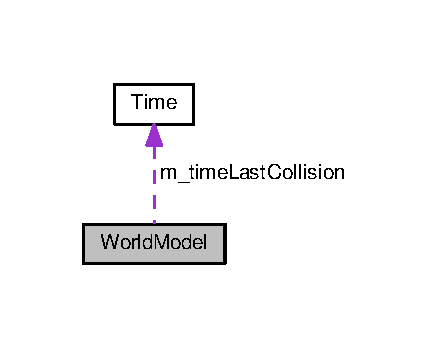
\includegraphics[width=206pt]{classWorldModel__coll__graph}
\end{center}
\end{figure}
\subsection*{Public Member Functions}
\begin{DoxyCompactItemize}
\item 
void \hyperlink{classWorldModel_a3c1f8adae4749937793f2e817987e55c}{set\+Time\+Last\+Catch} (\hyperlink{classTime}{Time} time)
\item 
int \hyperlink{classWorldModel_a8c574b586adecc5efa5c14f70dd2428b}{get\+Time\+Since\+Last\+Catch} ()
\item 
bool \hyperlink{classWorldModel_a9510256471538fe7e058950f26719122}{set\+Time\+Last\+Referee\+Message} (\hyperlink{classTime}{Time} time)
\item 
\hyperlink{classTime}{Time} \hyperlink{classWorldModel_ae6e6c4d6bdc2eca41a53cc79012d9898}{get\+Time\+Last\+Referee\+Message} ()
\item 
\hyperlink{classTime}{Time} \hyperlink{classWorldModel_a45fe68d69b6cc61cc6fdde86285d1ef5}{get\+Current\+Time} ()
\item 
int \hyperlink{classWorldModel_af3a4bb117a266363294808eed8b17b8b}{get\+Current\+Cycle} ()
\item 
bool \hyperlink{classWorldModel_abacf169ec2543f58e49031a2db3a2ab0}{is\+Time\+Stopped} ()
\item 
bool \hyperlink{classWorldModel_ad91e55d92db27dfd8bf7f503d8a14870}{is\+Last\+Message\+See} () const 
\item 
\hyperlink{classTime}{Time} \hyperlink{classWorldModel_a550156ab8e0a1f8f7c8d303cf93197d6}{get\+Time\+Last\+See\+Global\+Message} () const 
\item 
bool \hyperlink{classWorldModel_a5124cb6bdfeb473d06cf82c6cb79ab59}{set\+Time\+Last\+See\+Global\+Message} (\hyperlink{classTime}{Time} time)
\item 
\hyperlink{classTime}{Time} \hyperlink{classWorldModel_a4b7da103f0bc02ea1916e013aec2ae0d}{get\+Time\+Last\+See\+Message} () const 
\item 
\hyperlink{classTime}{Time} \hyperlink{classWorldModel_a482d61e23cc96e44562aa05781b32ab6}{get\+Time\+Last\+Recv\+See\+Message} () const 
\item 
bool \hyperlink{classWorldModel_aa21a08e85cf8ad026f3576ebc7c5a019}{set\+Time\+Last\+See\+Message} (\hyperlink{classTime}{Time} time)
\item 
\hyperlink{classTime}{Time} \hyperlink{classWorldModel_ad04adf9d3950663d605c5b2e15842626}{get\+Time\+Last\+Sense\+Message} () const 
\item 
\hyperlink{classTime}{Time} \hyperlink{classWorldModel_a39f27747324319b951a5eae8000f329a}{get\+Time\+Last\+Recv\+Sense\+Message} () const 
\item 
bool \hyperlink{classWorldModel_a52f59531cc7dccc043860c3f27a35a62}{set\+Time\+Last\+Sense\+Message} (\hyperlink{classTime}{Time} time)
\item 
\hyperlink{classTime}{Time} \hyperlink{classWorldModel_a3fe98cced0baea823e85c608785ee409}{get\+Time\+Last\+Hear\+Message} () const 
\item 
bool \hyperlink{classWorldModel_a2229c8f2e51c6b01a1f2ed6c09fe8636}{set\+Time\+Last\+Hear\+Message} (\hyperlink{classTime}{Time} time)
\item 
int \hyperlink{classWorldModel_af3318df1cbaf0c37db40b443b465e544}{get\+Player\+Number} () const 
\item 
bool \hyperlink{classWorldModel_aff5c37029df20b3190daed0d98031d49}{set\+Player\+Number} (int i)
\item 
\hyperlink{SoccerTypes_8h_a8e9b8119c00121a197203aca01d5b090}{SideT} \hyperlink{classWorldModel_a3f7abf17ee3e6920e45458d8fff82369}{get\+Side} () const 
\item 
bool \hyperlink{classWorldModel_af2fd2551973c5249ae85eab8222c455a}{set\+Side} (\hyperlink{SoccerTypes_8h_a8e9b8119c00121a197203aca01d5b090}{SideT} s)
\item 
const char $\ast$ \hyperlink{classWorldModel_ae2797273ce1b38d7e27306b9c9137e77}{get\+Team\+Name} () const 
\item 
bool \hyperlink{classWorldModel_ae2db1a838b75aea3d511401373bc0c86}{set\+Team\+Name} (char $\ast$str)
\item 
\hyperlink{SoccerTypes_8h_a471f1cfaf71f78e444ff420bb6646815}{Play\+ModeT} \hyperlink{classWorldModel_a78be826ce4ec8e13ee6d632bd0c32a7f}{get\+Play\+Mode} () const 
\item 
bool \hyperlink{classWorldModel_a7621ef9896c11cc442c1e043853b3567}{set\+Play\+Mode} (\hyperlink{SoccerTypes_8h_a471f1cfaf71f78e444ff420bb6646815}{Play\+ModeT} pm)
\item 
int \hyperlink{classWorldModel_a89ee8db585a4e9a0d1791d16e73bae98}{get\+Goal\+Diff} () const 
\item 
int \hyperlink{classWorldModel_ad5153a60aaad7c1c3405e43a25437f85}{add\+One\+To\+Goal\+Diff} ()
\item 
int \hyperlink{classWorldModel_a74df9bd4079aebd4648cb3cf62d9b5e2}{subtract\+One\+From\+Goal\+Diff} ()
\item 
int \hyperlink{classWorldModel_ab19576502fec85e5bcefe0a48fb130b6}{get\+Nr\+Of\+Commands} (\hyperlink{SoccerTypes_8h_ac986daf8a835e88572b79bcb63f5bbd5}{CommandT} c) const 
\item 
bool \hyperlink{classWorldModel_aaf094a670987e0a2b6c2f10c1e67f78b}{set\+Nr\+Of\+Commands} (\hyperlink{SoccerTypes_8h_ac986daf8a835e88572b79bcb63f5bbd5}{CommandT} c, int i)
\item 
\hyperlink{classTime}{Time} \hyperlink{classWorldModel_a93774177d5b76ab15e570f525849a6c3}{get\+Time\+Check\+Ball} () const 
\item 
bool \hyperlink{classWorldModel_a2b91f0042e6308b9d77412574af621f9}{set\+Time\+Check\+Ball} (\hyperlink{classTime}{Time} time)
\item 
\hyperlink{SoccerTypes_8h_aaeea770261a090c519643331173a327f}{Ball\+StatusT} \hyperlink{classWorldModel_a1394f01c0b698e94287247365e4e166b}{get\+Check\+Ball\+Status} () const 
\item 
bool \hyperlink{classWorldModel_a20d3184a5442370604f1f95bf4d5149e}{set\+Check\+Ball\+Status} (\hyperlink{SoccerTypes_8h_aaeea770261a090c519643331173a327f}{Ball\+StatusT} bs)
\item 
bool \hyperlink{classWorldModel_ab59f6cce3f520b0c07ce204a2a308fa2}{get\+Recv\+Think} ()
\item 
char $\ast$ \hyperlink{classWorldModel_adf4b82d91b2fa27ec82a269591f83548}{get\+Communication\+String} ()
\item 
bool \hyperlink{classWorldModel_af9cbc9830c16e98bade319f2efa953f9}{set\+Communication\+String} (const char $\ast$srt)
\item 
\hyperlink{SoccerTypes_8h_ad4b701fa66e7d26c054ed15b7820c77c}{ObjectT} \hyperlink{classWorldModel_a6fe3d09559d998400a4a898c473d4e07}{get\+Object\+Focus} ()
\item 
bool \hyperlink{classWorldModel_aac2a217b01cb11c9215180343549b0a6}{set\+Object\+Focus} (\hyperlink{SoccerTypes_8h_ad4b701fa66e7d26c054ed15b7820c77c}{ObjectT} obj)
\item 
\hyperlink{SoccerTypes_8h_ad4b701fa66e7d26c054ed15b7820c77c}{ObjectT} \hyperlink{classWorldModel_ae654ea58ca675dc1a38b649078577e12}{iterate\+Object\+Start} (int \&i\+Index, \hyperlink{SoccerTypes_8h_a30481b85f5315bc8f0d7a9e0468ea81f}{Object\+SetT} g, double d\+Conf=-\/1.\+0, bool b\+Forward=false)
\item 
\hyperlink{SoccerTypes_8h_ad4b701fa66e7d26c054ed15b7820c77c}{ObjectT} \hyperlink{classWorldModel_a8abd73a5fad17be2ea6d1f8522f51a0c}{iterate\+Object\+Next} (int \&i\+Index, \hyperlink{SoccerTypes_8h_a30481b85f5315bc8f0d7a9e0468ea81f}{Object\+SetT} g, double d\+Conf=-\/1.\+0, bool b\+Forward=false)
\item 
void \hyperlink{classWorldModel_a14592270aaec3966e8aef21747088f85}{iterate\+Object\+Done} (int \&i\+Index)
\item 
\hyperlink{SoccerTypes_8h_ad4b701fa66e7d26c054ed15b7820c77c}{ObjectT} \hyperlink{classWorldModel_a6ba702f3002dcb20834a60f0b6a71b67}{get\+Agent\+Object\+Type} () const 
\item 
int {\bfseries get\+Agent\+Index} () const \hypertarget{classWorldModel_a4f42041187089b28942129cd90b469b1}{}\label{classWorldModel_a4f42041187089b28942129cd90b469b1}

\item 
bool \hyperlink{classWorldModel_ab8b73d5348cca6a5e5ead46fe11ea19c}{set\+Agent\+Object\+Type} (\hyperlink{SoccerTypes_8h_ad4b701fa66e7d26c054ed15b7820c77c}{ObjectT} o)
\item 
\hyperlink{Geometry_8h_a6bfe02ae9bb185092902092561ab2865}{Ang\+Deg} \hyperlink{classWorldModel_a50b0a5e0de9147403caac0422addfdf9}{get\+Agent\+Body\+Angle\+Rel\+To\+Neck} () const 
\item 
\hyperlink{Geometry_8h_a6bfe02ae9bb185092902092561ab2865}{Ang\+Deg} \hyperlink{classWorldModel_a82245a1e3be23906608f29875cf361e1}{get\+Agent\+Global\+Neck\+Angle} () const 
\item 
\hyperlink{Geometry_8h_a6bfe02ae9bb185092902092561ab2865}{Ang\+Deg} \hyperlink{classWorldModel_abf87c4c8c5134db3af7cb5cb234428f1}{get\+Agent\+Global\+Body\+Angle} ()
\item 
\hyperlink{classStamina}{Stamina} \hyperlink{classWorldModel_a1517e5ae37e99ad69ea0a682caa9b25f}{get\+Agent\+Stamina} () const 
\item 
\hyperlink{SoccerTypes_8h_a30c890a1436546403a8d03667c70a94d}{Tired\+NessT} \hyperlink{classWorldModel_ae2b8b9ec3c42c708c9390545a33d2136}{get\+Agent\+Tired\+Ness} () const 
\item 
double \hyperlink{classWorldModel_a065e49c493ef65dc15d3bc77ec9cb920}{get\+Agent\+Effort} () const 
\item 
\hyperlink{classVecPosition}{Vec\+Position} \hyperlink{classWorldModel_a27c04feabe6a8473a8706299872293d7}{get\+Agent\+Global\+Velocity} () const 
\item 
double \hyperlink{classWorldModel_a78300aff00a8af184034826bebe75a19}{get\+Agent\+Speed} () const 
\item 
\hyperlink{classVecPosition}{Vec\+Position} \hyperlink{classWorldModel_a9421973b35ecbfbd881da9fd61016ada}{get\+Agent\+Global\+Position} () const 
\item 
bool \hyperlink{classWorldModel_a97068fe7fc6b358282197562ca5ab9ef}{set\+Agent\+View\+Angle} (\hyperlink{SoccerTypes_8h_ade95094b8e117801bea82ec390cccf64}{View\+AngleT} va)
\item 
\hyperlink{SoccerTypes_8h_ade95094b8e117801bea82ec390cccf64}{View\+AngleT} \hyperlink{classWorldModel_a8688f07b8402dfa9d998428eecae12e5}{get\+Agent\+View\+Angle} () const 
\item 
bool \hyperlink{classWorldModel_a16db12306101bc578c994a4e0ed8f6e8}{set\+Agent\+View\+Quality} (\hyperlink{SoccerTypes_8h_a5ae52e4e8062de90b118eacb03e99906}{View\+QualityT} vq)
\item 
\hyperlink{SoccerTypes_8h_a5ae52e4e8062de90b118eacb03e99906}{View\+QualityT} \hyperlink{classWorldModel_a583f8e59909e69d735ec850cc2732b63}{get\+Agent\+View\+Quality} () const 
\item 
double \hyperlink{classWorldModel_a6bf043449a94180a69e6836ed168e2e0}{get\+Agent\+View\+Frequency} (\hyperlink{SoccerTypes_8h_ade95094b8e117801bea82ec390cccf64}{View\+AngleT} va=\hyperlink{SoccerTypes_8h_ade95094b8e117801bea82ec390cccf64a2d8d518dae5e46e37c50ba929632665e}{V\+A\+\_\+\+I\+L\+L\+E\+G\+AL}, \hyperlink{SoccerTypes_8h_a5ae52e4e8062de90b118eacb03e99906}{View\+QualityT} vq=\hyperlink{SoccerTypes_8h_a5ae52e4e8062de90b118eacb03e99906aa69afb741ab1ef76033275d430ba7316}{V\+Q\+\_\+\+I\+L\+L\+E\+G\+AL})
\item 
bool \hyperlink{classWorldModel_a2d11d5239b4d0f2ac642f5a4588ef3c7}{get\+Agent\+Arm\+Movable} ()
\item 
\hyperlink{classVecPosition}{Vec\+Position} \hyperlink{classWorldModel_a50364564ae449a3a6246d4ac19c13a0b}{get\+Agent\+Arm\+Position} ()
\item 
int \hyperlink{classWorldModel_af03b1cbc646112a7fb4ddc0e5f037655}{get\+Agent\+Arm\+Expires} ()
\item 
\hyperlink{classVecPosition}{Vec\+Position} \hyperlink{classWorldModel_a4b64112d8c190f498c30a3f92cecf1c5}{get\+Ball\+Pos} ()
\item 
double \hyperlink{classWorldModel_a87ce5cf345fa0e3425c07154f4b30ca9}{get\+Ball\+Speed} ()
\item 
\hyperlink{Geometry_8h_a6bfe02ae9bb185092902092561ab2865}{Ang\+Deg} \hyperlink{classWorldModel_af13ef5d3f0794ed26a2d33e9e37b891a}{get\+Ball\+Direction} ()
\item 
\hyperlink{classTime}{Time} \hyperlink{classWorldModel_a861358fabbbff75d45a292ec31bce618}{get\+Time\+Global\+Position} (\hyperlink{SoccerTypes_8h_ad4b701fa66e7d26c054ed15b7820c77c}{ObjectT} o)
\item 
\hyperlink{classVecPosition}{Vec\+Position} \hyperlink{classWorldModel_a7f9eb0f6a54e6892aa30b397fed933a0}{get\+Global\+Position} (\hyperlink{SoccerTypes_8h_ad4b701fa66e7d26c054ed15b7820c77c}{ObjectT} o)
\item 
\hyperlink{classTime}{Time} \hyperlink{classWorldModel_ad6de27161c99a1f64ab226e260749031}{get\+Time\+Global\+Velocity} (\hyperlink{SoccerTypes_8h_ad4b701fa66e7d26c054ed15b7820c77c}{ObjectT} o)
\item 
\hyperlink{classVecPosition}{Vec\+Position} \hyperlink{classWorldModel_a528a52e72fdda936ff13ace88e933fd2}{get\+Global\+Velocity} (\hyperlink{SoccerTypes_8h_ad4b701fa66e7d26c054ed15b7820c77c}{ObjectT} o)
\item 
double \hyperlink{classWorldModel_a67418992805502114ef6cf7b6fb227b4}{get\+Relative\+Distance} (\hyperlink{SoccerTypes_8h_ad4b701fa66e7d26c054ed15b7820c77c}{ObjectT} o)
\item 
\hyperlink{classVecPosition}{Vec\+Position} \hyperlink{classWorldModel_a3f099caeac767241772a7ab5c131e550}{get\+Relative\+Position} (\hyperlink{SoccerTypes_8h_ad4b701fa66e7d26c054ed15b7820c77c}{ObjectT} o)
\item 
\hyperlink{Geometry_8h_a6bfe02ae9bb185092902092561ab2865}{Ang\+Deg} \hyperlink{classWorldModel_a91e023af096939d235073a37184bd8ca}{get\+Relative\+Angle} (\hyperlink{SoccerTypes_8h_ad4b701fa66e7d26c054ed15b7820c77c}{ObjectT} o, bool b\+With\+Body=false)
\item 
\hyperlink{classTime}{Time} \hyperlink{classWorldModel_af240e87b4270f09d68f19e365aa9e107}{get\+Time\+Global\+Angles} (\hyperlink{SoccerTypes_8h_ad4b701fa66e7d26c054ed15b7820c77c}{ObjectT} o)
\item 
\hyperlink{Geometry_8h_a6bfe02ae9bb185092902092561ab2865}{Ang\+Deg} \hyperlink{classWorldModel_a954452ec05deb2deda360332bb281cb4}{get\+Global\+Body\+Angle} (\hyperlink{SoccerTypes_8h_ad4b701fa66e7d26c054ed15b7820c77c}{ObjectT} o)
\item 
\hyperlink{Geometry_8h_a6bfe02ae9bb185092902092561ab2865}{Ang\+Deg} \hyperlink{classWorldModel_a8726a2fe3e7f439f64f44b9e4b67fded}{get\+Global\+Neck\+Angle} (\hyperlink{SoccerTypes_8h_ad4b701fa66e7d26c054ed15b7820c77c}{ObjectT} o)
\item 
\hyperlink{Geometry_8h_a6bfe02ae9bb185092902092561ab2865}{Ang\+Deg} \hyperlink{classWorldModel_a2aae1f22b1c60e20541979672397b46e}{get\+Global\+Angle} (\hyperlink{SoccerTypes_8h_ad4b701fa66e7d26c054ed15b7820c77c}{ObjectT} o)
\item 
double \hyperlink{classWorldModel_a243d6facc47a26066fb4e85994d00d9f}{get\+Confidence} (\hyperlink{SoccerTypes_8h_ad4b701fa66e7d26c054ed15b7820c77c}{ObjectT} o)
\item 
bool \hyperlink{classWorldModel_ae3125978959d41749db05c9d82591c92}{is\+Known\+Player} (\hyperlink{SoccerTypes_8h_ad4b701fa66e7d26c054ed15b7820c77c}{ObjectT} o)
\item 
\hyperlink{SoccerTypes_8h_ad4b701fa66e7d26c054ed15b7820c77c}{ObjectT} \hyperlink{classWorldModel_a8772d5bfb62c295ccf95f7c874f239de}{get\+Opp\+Goalie\+Type} ()
\item 
\hyperlink{SoccerTypes_8h_ad4b701fa66e7d26c054ed15b7820c77c}{ObjectT} \hyperlink{classWorldModel_a739d656a926dd290b93f4b185a76d2ad}{get\+Own\+Goalie\+Type} ()
\item 
\hyperlink{classTime}{Time} \hyperlink{classWorldModel_ac31101a94b46dc1cd2e4eeee034ae484}{get\+Time\+Last\+Seen} (\hyperlink{SoccerTypes_8h_ad4b701fa66e7d26c054ed15b7820c77c}{ObjectT} o)
\item 
\hyperlink{classTime}{Time} \hyperlink{classWorldModel_ae0bf4d9e4cc0c80924b735129dfbf5f1}{get\+Time\+Change\+Information} (\hyperlink{SoccerTypes_8h_ad4b701fa66e7d26c054ed15b7820c77c}{ObjectT} o)
\item 
\hyperlink{classVecPosition}{Vec\+Position} \hyperlink{classWorldModel_ae6fc1eed814f23445e2dcfd0cd7bf76f}{get\+Global\+Position\+Last\+See} (\hyperlink{SoccerTypes_8h_ad4b701fa66e7d26c054ed15b7820c77c}{ObjectT} o)
\item 
\hyperlink{classTime}{Time} \hyperlink{classWorldModel_a978165cd5c06285934b681d2a8d415c8}{get\+Time\+Global\+Position\+Last\+See} (\hyperlink{SoccerTypes_8h_ad4b701fa66e7d26c054ed15b7820c77c}{ObjectT} o)
\item 
\hyperlink{classVecPosition}{Vec\+Position} \hyperlink{classWorldModel_aae40b5b85c4961e3f12d7b282b2bcd0d}{get\+Global\+Velocity\+Last\+See} (\hyperlink{SoccerTypes_8h_ad4b701fa66e7d26c054ed15b7820c77c}{ObjectT} o)
\item 
\hyperlink{Geometry_8h_a6bfe02ae9bb185092902092561ab2865}{Ang\+Deg} \hyperlink{classWorldModel_ac86dc89c52b97048e818438af8407fa4}{get\+Global\+Body\+Angle\+Last\+See} (\hyperlink{SoccerTypes_8h_ad4b701fa66e7d26c054ed15b7820c77c}{ObjectT} o)
\item 
int \hyperlink{classWorldModel_a9df498cb39cb7bca374b14bc1c6975f3}{get\+Tackle\+Expires} (\hyperlink{SoccerTypes_8h_ad4b701fa66e7d26c054ed15b7820c77c}{ObjectT} o=\hyperlink{SoccerTypes_8h_ad4b701fa66e7d26c054ed15b7820c77cae887ec2051f19c0708a9a34df06e87a9}{O\+B\+J\+E\+C\+T\+\_\+\+I\+L\+L\+E\+G\+AL})
\item 
int \hyperlink{classWorldModel_a95613f3a14c87788da3a2b5c280406df}{get\+Cycle\+Last\+Tackle} (\hyperlink{SoccerTypes_8h_ad4b701fa66e7d26c054ed15b7820c77c}{ObjectT} o=\hyperlink{SoccerTypes_8h_ad4b701fa66e7d26c054ed15b7820c77cae887ec2051f19c0708a9a34df06e87a9}{O\+B\+J\+E\+C\+T\+\_\+\+I\+L\+L\+E\+G\+AL})
\item 
int \hyperlink{classWorldModel_a91ddf471f01abfeeef72434599be3270}{get\+Cycle\+Last\+Kick} (\hyperlink{SoccerTypes_8h_ad4b701fa66e7d26c054ed15b7820c77c}{ObjectT} o=\hyperlink{SoccerTypes_8h_ad4b701fa66e7d26c054ed15b7820c77cae887ec2051f19c0708a9a34df06e87a9}{O\+B\+J\+E\+C\+T\+\_\+\+I\+L\+L\+E\+G\+AL})
\item 
void \hyperlink{classWorldModel_a2ee86d76a5e2e126cc4be10ef96e1f9c}{set\+Cycle\+Agent\+Last\+Tackle} ()
\item 
\hyperlink{Geometry_8h_a6bfe02ae9bb185092902092561ab2865}{Ang\+Deg} \hyperlink{classWorldModel_a679dea1dcc5ed50babbec89484cf9b4a}{get\+Global\+Arm\+Direction} (\hyperlink{SoccerTypes_8h_ad4b701fa66e7d26c054ed15b7820c77c}{ObjectT} o)
\item 
\hyperlink{classTime}{Time} \hyperlink{classWorldModel_aa1f30271cf7e81bb431d9ee690580e0f}{get\+Time\+Global\+Arm\+Direction} (\hyperlink{SoccerTypes_8h_ad4b701fa66e7d26c054ed15b7820c77c}{ObjectT} o)
\item 
double \hyperlink{classWorldModel_a0227bcbd12548e413ae969f364b99e20}{get\+Prob\+Tackle\+Succeeds} (\hyperlink{SoccerTypes_8h_ad4b701fa66e7d26c054ed15b7820c77c}{ObjectT} o=\hyperlink{SoccerTypes_8h_ad4b701fa66e7d26c054ed15b7820c77cae887ec2051f19c0708a9a34df06e87a9}{O\+B\+J\+E\+C\+T\+\_\+\+I\+L\+L\+E\+G\+AL}, int i\+Extra\+Cycles=0, \hyperlink{classVecPosition}{Vec\+Position} $\ast$pos=N\+U\+LL)
\item 
double \hyperlink{classWorldModel_ac479947397649bb63ada2192778a1601}{get\+Prob\+Tackle\+Closest\+Opp} (int i\+Extra\+Cycles=0)
\item 
list$<$ \hyperlink{SoccerTypes_8h_ad4b701fa66e7d26c054ed15b7820c77c}{ObjectT} $>$ \hyperlink{classWorldModel_aafa0b244a2ae9bdcefa32776ab5480ce}{get\+List\+Close\+Opponents} (\hyperlink{classVecPosition}{Vec\+Position} pos, double d\+Dist=15)
\item 
bool \hyperlink{classWorldModel_acb2453fc64d6e816650d9bb6e36f886f}{set\+Is\+Known\+Player} (\hyperlink{SoccerTypes_8h_ad4b701fa66e7d26c054ed15b7820c77c}{ObjectT} o, bool \hyperlink{classWorldModel_ae3125978959d41749db05c9d82591c92}{is\+Known\+Player})
\item 
bool \hyperlink{classWorldModel_aefb0ad56b245318bf638bcb959688854}{set\+Time\+Last\+Seen} (\hyperlink{SoccerTypes_8h_ad4b701fa66e7d26c054ed15b7820c77c}{ObjectT} o, \hyperlink{classTime}{Time} time)
\item 
bool \hyperlink{classWorldModel_ac35cabe1b94a47e4f60e23dd8040cfbc}{set\+Hetero\+Player\+Type} (\hyperlink{SoccerTypes_8h_ad4b701fa66e7d26c054ed15b7820c77c}{ObjectT} o, int i\+Player)
\item 
\hyperlink{SoccerTypes_8h_a88daf580b042467ccd4098107cffc718}{PlayerT} \hyperlink{classWorldModel_add51d2f1797b97e601b532d083b267d7}{get\+Player\+Type} (\hyperlink{SoccerTypes_8h_ad4b701fa66e7d26c054ed15b7820c77c}{ObjectT} o=\hyperlink{SoccerTypes_8h_ad4b701fa66e7d26c054ed15b7820c77cae887ec2051f19c0708a9a34df06e87a9}{O\+B\+J\+E\+C\+T\+\_\+\+I\+L\+L\+E\+G\+AL})
\item 
bool \hyperlink{classWorldModel_a914ceb6699a51c4cb04f9d19f75ddda0}{is\+In\+Player\+Set} (\hyperlink{SoccerTypes_8h_ad4b701fa66e7d26c054ed15b7820c77c}{ObjectT} o, \hyperlink{SoccerTypes_8h_afbb545db37d2371bdcf6936de7504d00}{Player\+SetT} ps)
\item 
\hyperlink{classVecPosition}{Vec\+Position} \hyperlink{classWorldModel_a165727b8afb79369833e6cc741c43ebf}{get\+Pos\+Opponent\+Goal} ()
\item 
\hyperlink{classVecPosition}{Vec\+Position} \hyperlink{classWorldModel_a22b5446854868a9335c4a72c46ef5c09}{get\+Pos\+Own\+Goal} ()
\item 
double \hyperlink{classWorldModel_ab213a55a97c5abf0c8ae8935588668ab}{get\+Rel\+Distance\+Opponent\+Goal} ()
\item 
\hyperlink{Geometry_8h_a6bfe02ae9bb185092902092561ab2865}{Ang\+Deg} \hyperlink{classWorldModel_a4993438af6965524722f7bb3047c2e83}{get\+Rel\+Angle\+Opponent\+Goal} ()
\item 
\hyperlink{SoccerTypes_8h_ad4b701fa66e7d26c054ed15b7820c77c}{ObjectT} \hyperlink{classWorldModel_a78874ff4ace4f07d2394ff3f20214448}{get\+Last\+Opponent\+Defender} (double $\ast$dX=N\+U\+LL)
\item 
\hyperlink{classHeteroPlayerSettings}{Hetero\+Player\+Settings} \hyperlink{classWorldModel_a06c4a9c272445a0c9b8b816c3cfede97}{get\+Info\+Hetero\+Player} (int i\+Index)
\item 
\hyperlink{classHeteroPlayerSettings}{Hetero\+Player\+Settings} \hyperlink{classWorldModel_afeaf0988a5e402a5425faff1e9846cfa}{get\+Hetero\+Info\+Player} (\hyperlink{SoccerTypes_8h_ad4b701fa66e7d26c054ed15b7820c77c}{ObjectT} obj)
\item 
int \hyperlink{classWorldModel_adc43f0254d058adb328029bbeac2375e}{get\+Hetero\+Player\+Type} (\hyperlink{SoccerTypes_8h_ad4b701fa66e7d26c054ed15b7820c77c}{ObjectT} obj)
\item 
bool \hyperlink{classWorldModel_a445c9f350b9f2710e20f677adacab6cb}{set\+Substituted\+Opp} (\hyperlink{SoccerTypes_8h_ad4b701fa66e7d26c054ed15b7820c77c}{ObjectT} obj)
\item 
\hyperlink{SoccerTypes_8h_ad4b701fa66e7d26c054ed15b7820c77c}{ObjectT} \hyperlink{classWorldModel_a4ae7ccc6839b27f514fbedfee53d01df}{get\+Substituted\+Opp} ()
\item 
double \hyperlink{classWorldModel_aa3818f9d180f20a434ccd8a532b291ba}{get\+Dash\+Power\+Rate} (\hyperlink{SoccerTypes_8h_ad4b701fa66e7d26c054ed15b7820c77c}{ObjectT} obj)
\item 
double \hyperlink{classWorldModel_a9c36f32a0c226211b99e71b05b699785}{get\+Player\+Speed\+Max} (\hyperlink{SoccerTypes_8h_ad4b701fa66e7d26c054ed15b7820c77c}{ObjectT} obj)
\item 
double \hyperlink{classWorldModel_a5330e20bc5ba4d5126145675012ce167}{get\+Player\+Decay} (\hyperlink{SoccerTypes_8h_ad4b701fa66e7d26c054ed15b7820c77c}{ObjectT} obj)
\item 
double \hyperlink{classWorldModel_a98caf9a024851a757ac76a2f0847cafe}{get\+Maximal\+Kick\+Dist} (\hyperlink{SoccerTypes_8h_ad4b701fa66e7d26c054ed15b7820c77c}{ObjectT} obj)
\item 
double \hyperlink{classWorldModel_a77769a7b6b8d31fb20621ac39bcd197e}{get\+Stamina\+Inc\+Max} (\hyperlink{SoccerTypes_8h_ad4b701fa66e7d26c054ed15b7820c77c}{ObjectT} obj)
\item 
double \hyperlink{classWorldModel_a2089004a819c9169be67b7b650cb89fa}{get\+Player\+Size} (\hyperlink{SoccerTypes_8h_ad4b701fa66e7d26c054ed15b7820c77c}{ObjectT} obj)
\item 
double \hyperlink{classWorldModel_a628b06329ef0ec1f761b0d5dc34d986c}{get\+Inertia\+Moment} (\hyperlink{SoccerTypes_8h_ad4b701fa66e7d26c054ed15b7820c77c}{ObjectT} obj)
\item 
double \hyperlink{classWorldModel_ad1167159c2477d5ea2f9ad4ef9879e69}{get\+Effort\+Max} (\hyperlink{SoccerTypes_8h_ad4b701fa66e7d26c054ed15b7820c77c}{ObjectT} obj)
\item 
double \hyperlink{classWorldModel_a109e48e6a2d2524af5058306da0a7a1b}{get\+Effective\+Max\+Speed} (\hyperlink{SoccerTypes_8h_ad4b701fa66e7d26c054ed15b7820c77c}{ObjectT} obj, bool b\+With\+Noise=false)
\item 
bool \hyperlink{classWorldModel_a9c6ca2d978c49152eb6acba91f27fbd0}{is\+Queued\+Action\+Performed} ()
\item 
bool \hyperlink{classWorldModel_ad3a6e69921dfea30e9c4b0097c276314}{is\+Free\+Kick\+Us} (\hyperlink{SoccerTypes_8h_a471f1cfaf71f78e444ff420bb6646815}{Play\+ModeT} pm=\hyperlink{SoccerTypes_8h_a471f1cfaf71f78e444ff420bb6646815a90ccb9da3d7f1339f9bce928de2f3c60}{P\+M\+\_\+\+I\+L\+L\+E\+G\+AL})
\item 
bool \hyperlink{classWorldModel_a566818a13e6cb99706d811446517cf97}{is\+Free\+Kick\+Them} (\hyperlink{SoccerTypes_8h_a471f1cfaf71f78e444ff420bb6646815}{Play\+ModeT} pm=\hyperlink{SoccerTypes_8h_a471f1cfaf71f78e444ff420bb6646815a90ccb9da3d7f1339f9bce928de2f3c60}{P\+M\+\_\+\+I\+L\+L\+E\+G\+AL})
\item 
bool \hyperlink{classWorldModel_a52f30ff6f5eb5f72544ce68173f116be}{is\+Corner\+Kick\+Us} (\hyperlink{SoccerTypes_8h_a471f1cfaf71f78e444ff420bb6646815}{Play\+ModeT} pm=\hyperlink{SoccerTypes_8h_a471f1cfaf71f78e444ff420bb6646815a90ccb9da3d7f1339f9bce928de2f3c60}{P\+M\+\_\+\+I\+L\+L\+E\+G\+AL})
\item 
bool \hyperlink{classWorldModel_aae69dd20181df945f9ccfc7bd92e0cd1}{is\+Corner\+Kick\+Them} (\hyperlink{SoccerTypes_8h_a471f1cfaf71f78e444ff420bb6646815}{Play\+ModeT} pm=\hyperlink{SoccerTypes_8h_a471f1cfaf71f78e444ff420bb6646815a90ccb9da3d7f1339f9bce928de2f3c60}{P\+M\+\_\+\+I\+L\+L\+E\+G\+AL})
\item 
bool \hyperlink{classWorldModel_a159977aa40d36de8d8233d93f3347bf6}{is\+Offside\+Us} (\hyperlink{SoccerTypes_8h_a471f1cfaf71f78e444ff420bb6646815}{Play\+ModeT} pm=\hyperlink{SoccerTypes_8h_a471f1cfaf71f78e444ff420bb6646815a90ccb9da3d7f1339f9bce928de2f3c60}{P\+M\+\_\+\+I\+L\+L\+E\+G\+AL})
\item 
bool \hyperlink{classWorldModel_a9dc6a2dec9d1e36ac40244ab1e71d3ef}{is\+Offside\+Them} (\hyperlink{SoccerTypes_8h_a471f1cfaf71f78e444ff420bb6646815}{Play\+ModeT} pm=\hyperlink{SoccerTypes_8h_a471f1cfaf71f78e444ff420bb6646815a90ccb9da3d7f1339f9bce928de2f3c60}{P\+M\+\_\+\+I\+L\+L\+E\+G\+AL})
\item 
bool \hyperlink{classWorldModel_a627df5348d37359f7cbff24d9ea222a1}{is\+Kick\+In\+Us} (\hyperlink{SoccerTypes_8h_a471f1cfaf71f78e444ff420bb6646815}{Play\+ModeT} pm=\hyperlink{SoccerTypes_8h_a471f1cfaf71f78e444ff420bb6646815a90ccb9da3d7f1339f9bce928de2f3c60}{P\+M\+\_\+\+I\+L\+L\+E\+G\+AL})
\item 
bool \hyperlink{classWorldModel_ab88c24ce981f0b8a619c2ca05ca4ebf7}{is\+Kick\+In\+Them} (\hyperlink{SoccerTypes_8h_a471f1cfaf71f78e444ff420bb6646815}{Play\+ModeT} pm=\hyperlink{SoccerTypes_8h_a471f1cfaf71f78e444ff420bb6646815a90ccb9da3d7f1339f9bce928de2f3c60}{P\+M\+\_\+\+I\+L\+L\+E\+G\+AL})
\item 
bool \hyperlink{classWorldModel_a8b0927a2122cd775c8bd839ec76fb0fb}{is\+Free\+Kick\+Fault\+Us} (\hyperlink{SoccerTypes_8h_a471f1cfaf71f78e444ff420bb6646815}{Play\+ModeT} pm=\hyperlink{SoccerTypes_8h_a471f1cfaf71f78e444ff420bb6646815a90ccb9da3d7f1339f9bce928de2f3c60}{P\+M\+\_\+\+I\+L\+L\+E\+G\+AL})
\item 
bool \hyperlink{classWorldModel_ad7cf4809e53a5eb956cd5309c3d5de84}{is\+Free\+Kick\+Fault\+Them} (\hyperlink{SoccerTypes_8h_a471f1cfaf71f78e444ff420bb6646815}{Play\+ModeT} pm=\hyperlink{SoccerTypes_8h_a471f1cfaf71f78e444ff420bb6646815a90ccb9da3d7f1339f9bce928de2f3c60}{P\+M\+\_\+\+I\+L\+L\+E\+G\+AL})
\item 
bool \hyperlink{classWorldModel_aa0bb248f66d3537f33c223ee6e1ad487}{is\+Kick\+Off\+Us} (\hyperlink{SoccerTypes_8h_a471f1cfaf71f78e444ff420bb6646815}{Play\+ModeT} pm=\hyperlink{SoccerTypes_8h_a471f1cfaf71f78e444ff420bb6646815a90ccb9da3d7f1339f9bce928de2f3c60}{P\+M\+\_\+\+I\+L\+L\+E\+G\+AL})
\item 
bool \hyperlink{classWorldModel_a204c773ec45f00f6a8e25c23ed64cf54}{is\+Kick\+Off\+Them} (\hyperlink{SoccerTypes_8h_a471f1cfaf71f78e444ff420bb6646815}{Play\+ModeT} pm=\hyperlink{SoccerTypes_8h_a471f1cfaf71f78e444ff420bb6646815a90ccb9da3d7f1339f9bce928de2f3c60}{P\+M\+\_\+\+I\+L\+L\+E\+G\+AL})
\item 
bool \hyperlink{classWorldModel_a63f46981f1cbed5d92cc6fbd00795698}{is\+Back\+Pass\+Us} (\hyperlink{SoccerTypes_8h_a471f1cfaf71f78e444ff420bb6646815}{Play\+ModeT} pm=\hyperlink{SoccerTypes_8h_a471f1cfaf71f78e444ff420bb6646815a90ccb9da3d7f1339f9bce928de2f3c60}{P\+M\+\_\+\+I\+L\+L\+E\+G\+AL})
\item 
bool \hyperlink{classWorldModel_a9d469360064a305dbeffcb4dab90cec0}{is\+Back\+Pass\+Them} (\hyperlink{SoccerTypes_8h_a471f1cfaf71f78e444ff420bb6646815}{Play\+ModeT} pm=\hyperlink{SoccerTypes_8h_a471f1cfaf71f78e444ff420bb6646815a90ccb9da3d7f1339f9bce928de2f3c60}{P\+M\+\_\+\+I\+L\+L\+E\+G\+AL})
\item 
bool \hyperlink{classWorldModel_a4a84d1336526c6acfd05a1e329181490}{is\+Goal\+Kick\+Us} (\hyperlink{SoccerTypes_8h_a471f1cfaf71f78e444ff420bb6646815}{Play\+ModeT} pm=\hyperlink{SoccerTypes_8h_a471f1cfaf71f78e444ff420bb6646815a90ccb9da3d7f1339f9bce928de2f3c60}{P\+M\+\_\+\+I\+L\+L\+E\+G\+AL})
\item 
bool \hyperlink{classWorldModel_a397c747c73f21f2c6a5805872c7a954d}{is\+Goal\+Kick\+Them} (\hyperlink{SoccerTypes_8h_a471f1cfaf71f78e444ff420bb6646815}{Play\+ModeT} pm=\hyperlink{SoccerTypes_8h_a471f1cfaf71f78e444ff420bb6646815a90ccb9da3d7f1339f9bce928de2f3c60}{P\+M\+\_\+\+I\+L\+L\+E\+G\+AL})
\item 
bool \hyperlink{classWorldModel_a97bac37d2b77a03a54287e77854dcfb2}{is\+Before\+Kick\+Off} (\hyperlink{SoccerTypes_8h_a471f1cfaf71f78e444ff420bb6646815}{Play\+ModeT} pm=\hyperlink{SoccerTypes_8h_a471f1cfaf71f78e444ff420bb6646815a90ccb9da3d7f1339f9bce928de2f3c60}{P\+M\+\_\+\+I\+L\+L\+E\+G\+AL})
\item 
bool \hyperlink{classWorldModel_ae67af8a3828f06424ddc11c3f49b1383}{is\+Dead\+Ball\+Us} (\hyperlink{SoccerTypes_8h_a471f1cfaf71f78e444ff420bb6646815}{Play\+ModeT} pm=\hyperlink{SoccerTypes_8h_a471f1cfaf71f78e444ff420bb6646815a90ccb9da3d7f1339f9bce928de2f3c60}{P\+M\+\_\+\+I\+L\+L\+E\+G\+AL})
\item 
bool \hyperlink{classWorldModel_a0d931570ae04bc6541bf1fc1ed3c4b4c}{is\+Dead\+Ball\+Them} (\hyperlink{SoccerTypes_8h_a471f1cfaf71f78e444ff420bb6646815}{Play\+ModeT} pm=\hyperlink{SoccerTypes_8h_a471f1cfaf71f78e444ff420bb6646815a90ccb9da3d7f1339f9bce928de2f3c60}{P\+M\+\_\+\+I\+L\+L\+E\+G\+AL})
\item 
bool \hyperlink{classWorldModel_a975e41fff45b95bd39905a978b2820a3}{is\+Penalty\+Us} (\hyperlink{SoccerTypes_8h_a471f1cfaf71f78e444ff420bb6646815}{Play\+ModeT} pm=\hyperlink{SoccerTypes_8h_a471f1cfaf71f78e444ff420bb6646815a90ccb9da3d7f1339f9bce928de2f3c60}{P\+M\+\_\+\+I\+L\+L\+E\+G\+AL})
\item 
bool \hyperlink{classWorldModel_a1c227b5b56eb78ef9b4b6f4da2c3822e}{is\+Penalty\+Them} (\hyperlink{SoccerTypes_8h_a471f1cfaf71f78e444ff420bb6646815}{Play\+ModeT} pm=\hyperlink{SoccerTypes_8h_a471f1cfaf71f78e444ff420bb6646815a90ccb9da3d7f1339f9bce928de2f3c60}{P\+M\+\_\+\+I\+L\+L\+E\+G\+AL})
\item 
bool {\bfseries is\+Full\+State\+On} (\hyperlink{SoccerTypes_8h_a8e9b8119c00121a197203aca01d5b090}{SideT} s=\hyperlink{SoccerTypes_8h_a8e9b8119c00121a197203aca01d5b090a15a5449d2724d5cf4a7855b32888b24a}{S\+I\+D\+E\+\_\+\+I\+L\+L\+E\+G\+AL})\hypertarget{classWorldModel_ad1310e991df43785a769cfb9c89f2d8e}{}\label{classWorldModel_ad1310e991df43785a769cfb9c89f2d8e}

\item 
bool {\bfseries set\+Change\+View\+Command} (\hyperlink{classSoccerCommand}{Soccer\+Command} soc)\hypertarget{classWorldModel_a6c5c118dd8e2c4606346aa704e231c4d}{}\label{classWorldModel_a6c5c118dd8e2c4606346aa704e231c4d}

\item 
\hyperlink{classSoccerCommand}{Soccer\+Command} {\bfseries get\+Change\+View\+Command} ()\hypertarget{classWorldModel_ad380f8d4817c71cbb5378e30dc41d1f1}{}\label{classWorldModel_ad380f8d4817c71cbb5378e30dc41d1f1}

\item 
\hyperlink{SoccerTypes_8h_a8e9b8119c00121a197203aca01d5b090}{SideT} \hyperlink{classWorldModel_ad0475be2fdbfd61f02c65e035a2b4f2e}{get\+Side\+Penalty} ()
\item 
bool \hyperlink{classWorldModel_a4620a7851987e387254169b314be7a0b}{set\+Side\+Penalty} (\hyperlink{SoccerTypes_8h_a8e9b8119c00121a197203aca01d5b090}{SideT} side)
\item 
void \hyperlink{classWorldModel_a080e7eee476545958ffe1b257c70515a}{process\+See\+Global\+Info} (\hyperlink{SoccerTypes_8h_ad4b701fa66e7d26c054ed15b7820c77c}{ObjectT} o, \hyperlink{classTime}{Time} time, \hyperlink{classVecPosition}{Vec\+Position} pos, \hyperlink{classVecPosition}{Vec\+Position} vel, \hyperlink{Geometry_8h_a6bfe02ae9bb185092902092561ab2865}{Ang\+Deg} ang\+Body, \hyperlink{Geometry_8h_a6bfe02ae9bb185092902092561ab2865}{Ang\+Deg} ang\+Neck)
\item 
bool \hyperlink{classWorldModel_a116b826cf3be5a24af10f81195e67b48}{process\+New\+Agent\+Info} (\hyperlink{SoccerTypes_8h_a5ae52e4e8062de90b118eacb03e99906}{View\+QualityT} vq, \hyperlink{SoccerTypes_8h_ade95094b8e117801bea82ec390cccf64}{View\+AngleT} va, double d\+Stamina, double d\+Effort, double d\+Capacity, double d\+Speed, \hyperlink{Geometry_8h_a6bfe02ae9bb185092902092561ab2865}{Ang\+Deg} ang\+Speed, \hyperlink{Geometry_8h_a6bfe02ae9bb185092902092561ab2865}{Ang\+Deg} ang\+Head\+Angle, int i\+Tackle\+Expires, int i\+Arm\+Movable, int i\+Arm\+Expires, \hyperlink{classVecPosition}{Vec\+Position} pos\+Arm)
\item 
void \hyperlink{classWorldModel_adab20d0896f02bbd320da421858d9390}{process\+New\+Object\+Info} (\hyperlink{SoccerTypes_8h_ad4b701fa66e7d26c054ed15b7820c77c}{ObjectT} o, \hyperlink{classTime}{Time} time, double d\+Dist, int i\+Dir, double d\+Dist\+Change, double d\+Dir\+Change, \hyperlink{Geometry_8h_a6bfe02ae9bb185092902092561ab2865}{Ang\+Deg} ang\+Rel\+Body\+Ang, \hyperlink{Geometry_8h_a6bfe02ae9bb185092902092561ab2865}{Ang\+Deg} ang\+Rel\+Neck\+Ang, bool is\+Goalie, \hyperlink{SoccerTypes_8h_ad4b701fa66e7d26c054ed15b7820c77c}{ObjectT} obj\+Min, \hyperlink{SoccerTypes_8h_ad4b701fa66e7d26c054ed15b7820c77c}{ObjectT} obj\+Max, double d\+Point\+Dir, bool is\+Tackling, bool is\+Kicking)
\item 
bool \hyperlink{classWorldModel_ac842b5212372ede26fc484a46e331e20}{process\+Perfect\+Hear\+Info} (\hyperlink{SoccerTypes_8h_ad4b701fa66e7d26c054ed15b7820c77c}{ObjectT} o, \hyperlink{classVecPosition}{Vec\+Position} pos, double d\+Conf, bool b\+Is\+Goalie=0)
\item 
bool \hyperlink{classWorldModel_aeea7e051d12991733774038156b9f12f}{process\+Perfect\+Hear\+Info\+Ball} (\hyperlink{classVecPosition}{Vec\+Position} pos, \hyperlink{classVecPosition}{Vec\+Position} vel, double d\+Conf)
\item 
bool \hyperlink{classWorldModel_a06677f2292a72516ad3f40c3da35c120}{process\+Unsure\+Hear\+Info} (\hyperlink{SoccerTypes_8h_ad4b701fa66e7d26c054ed15b7820c77c}{ObjectT} o, \hyperlink{classVecPosition}{Vec\+Position} pos, double d\+Conf)
\item 
bool \hyperlink{classWorldModel_a538080bac7f2cc7a444bca6010bf88ad}{process\+New\+Hetero\+Player} (int i\+Index, double d\+Player\+Speed\+Max, double d\+Stamina\+Inc\+Max, double d\+Player\+Decay, double d\+Inertia\+Moment, double d\+Dash\+Power\+Rate, double d\+Player\+Size, double d\+Kickable\+Margin, double d\+Kick\+Rand, double d\+Extra\+Stamina, double d\+Effort\+Max, double d\+Effort\+Min)
\item 
void \hyperlink{classWorldModel_ac9ef88b9ea7fc0ab8cc4f3f85c75f370}{process\+Catched\+Ball} (\hyperlink{SoccerTypes_8h_abb5fa6e95f3a11e041200e983b2c2e4c}{Referee\+MessageT} rm, \hyperlink{classTime}{Time} time)
\item 
void \hyperlink{classWorldModel_ab8d90c2224cef9ee973cd76be056aca5}{process\+Queued\+Commands} (\hyperlink{classSoccerCommand}{Soccer\+Command} commands\mbox{[}$\,$\mbox{]}, int i\+Commands)
\item 
bool \hyperlink{classWorldModel_a356bbd919551bc73508e159a6d78f83a}{store\+Player\+Message} (int i\+Player, char $\ast$str\+Msg, int i\+Cycle)
\item 
bool \hyperlink{classWorldModel_a31197f8fd6b403fe0a39ff42a0f32278}{process\+Player\+Message} ()
\item 
bool {\bfseries process\+Recv\+Think} (bool b)\hypertarget{classWorldModel_ae95386449f880f0c28a809bcb19d703d}{}\label{classWorldModel_ae95386449f880f0c28a809bcb19d703d}

\item 
bool \hyperlink{classWorldModel_a6e00efb98c2a4c9d86f015f586cfd5e5}{update\+All} ()
\item 
bool \hyperlink{classWorldModel_a04698ceb985c59f068f7d70a362f92bc}{update\+After\+Sense\+Message} ()
\item 
void \hyperlink{classWorldModel_ac26e3777e83ad0bf7c6713148e358845}{map\+Unknown\+Players} (\hyperlink{classTime}{Time} time)
\item 
bool \hyperlink{classWorldModel_abca28bb43aefb07240561908056ec872}{update\+S\+S\+To\+Hetero\+Player\+Type} (int i\+Player\+Type)
\item 
bool \hyperlink{classWorldModel_a636fa9ad9af4c41994df195e561a1130}{reset\+Time\+Objects} ()
\item 
void \hyperlink{classWorldModel_a8bf2e3f9269eecaeee8b3bed10f13a4b}{remove\+Ghosts} ()
\item 
bool \hyperlink{classWorldModel_a19b844c1c20d409b3e85bb9ba03d6043}{predict\+State\+After\+Command} (\hyperlink{classSoccerCommand}{Soccer\+Command} com, \hyperlink{classVecPosition}{Vec\+Position} $\ast$pos, \hyperlink{classVecPosition}{Vec\+Position} $\ast$vel, \hyperlink{Geometry_8h_a6bfe02ae9bb185092902092561ab2865}{Ang\+Deg} $\ast$ang\+Global\+Body, \hyperlink{Geometry_8h_a6bfe02ae9bb185092902092561ab2865}{Ang\+Deg} $\ast$ang\+Global\+Neck, \hyperlink{SoccerTypes_8h_ad4b701fa66e7d26c054ed15b7820c77c}{ObjectT} obj=\hyperlink{SoccerTypes_8h_ad4b701fa66e7d26c054ed15b7820c77cae887ec2051f19c0708a9a34df06e87a9}{O\+B\+J\+E\+C\+T\+\_\+\+I\+L\+L\+E\+G\+AL}, \hyperlink{classStamina}{Stamina} $\ast$sta=N\+U\+LL)
\item 
bool \hyperlink{classWorldModel_a07fabc55d8c23a54b7179149505d1ff0}{predict\+Agent\+State\+After\+Command} (\hyperlink{classSoccerCommand}{Soccer\+Command} com, \hyperlink{classVecPosition}{Vec\+Position} $\ast$pos, \hyperlink{classVecPosition}{Vec\+Position} $\ast$vel, \hyperlink{Geometry_8h_a6bfe02ae9bb185092902092561ab2865}{Ang\+Deg} $\ast$ang\+Body, \hyperlink{Geometry_8h_a6bfe02ae9bb185092902092561ab2865}{Ang\+Deg} $\ast$ang\+Neck, \hyperlink{classStamina}{Stamina} $\ast$sta)
\item 
bool \hyperlink{classWorldModel_ae168921990f19b62faece4716b33e0ac}{predict\+Object\+State\+After\+Command} (\hyperlink{SoccerTypes_8h_ad4b701fa66e7d26c054ed15b7820c77c}{ObjectT} obj, \hyperlink{classSoccerCommand}{Soccer\+Command} com, \hyperlink{classVecPosition}{Vec\+Position} $\ast$pos, \hyperlink{classVecPosition}{Vec\+Position} $\ast$vel, \hyperlink{Geometry_8h_a6bfe02ae9bb185092902092561ab2865}{Ang\+Deg} $\ast$ang\+Body, \hyperlink{Geometry_8h_a6bfe02ae9bb185092902092561ab2865}{Ang\+Deg} $\ast$ang\+Neck, \hyperlink{classStamina}{Stamina} $\ast$sta)
\item 
\hyperlink{classVecPosition}{Vec\+Position} \hyperlink{classWorldModel_ac0247c0f31fcc19228e52e90ecac458b}{predict\+Agent\+Pos\+After\+Command} (\hyperlink{classSoccerCommand}{Soccer\+Command} com)
\item 
void \hyperlink{classWorldModel_ac9ab1bf0eca6ba5aa64a92395be823d1}{predict\+State\+After\+Dash} (double d\+Actual\+Power, \hyperlink{classVecPosition}{Vec\+Position} $\ast$pos, \hyperlink{classVecPosition}{Vec\+Position} $\ast$vel, \hyperlink{classStamina}{Stamina} $\ast$sta, double d\+Direction, \hyperlink{SoccerTypes_8h_ad4b701fa66e7d26c054ed15b7820c77c}{ObjectT} o=\hyperlink{SoccerTypes_8h_ad4b701fa66e7d26c054ed15b7820c77cae887ec2051f19c0708a9a34df06e87a9}{O\+B\+J\+E\+C\+T\+\_\+\+I\+L\+L\+E\+G\+AL})
\item 
void \hyperlink{classWorldModel_a2fc55368b1cf0abc06df0e8c10102859}{predict\+State\+After\+Turn} (\hyperlink{Geometry_8h_a6bfe02ae9bb185092902092561ab2865}{Ang\+Deg} d\+Send\+Angle, \hyperlink{classVecPosition}{Vec\+Position} $\ast$pos, \hyperlink{classVecPosition}{Vec\+Position} $\ast$vel, \hyperlink{Geometry_8h_a6bfe02ae9bb185092902092561ab2865}{Ang\+Deg} $\ast$ang\+Body, \hyperlink{Geometry_8h_a6bfe02ae9bb185092902092561ab2865}{Ang\+Deg} $\ast$ang\+Neck, \hyperlink{SoccerTypes_8h_ad4b701fa66e7d26c054ed15b7820c77c}{ObjectT} obj=\hyperlink{SoccerTypes_8h_ad4b701fa66e7d26c054ed15b7820c77cae887ec2051f19c0708a9a34df06e87a9}{O\+B\+J\+E\+C\+T\+\_\+\+I\+L\+L\+E\+G\+AL}, \hyperlink{classStamina}{Stamina} $\ast$sta=N\+U\+LL)
\item 
void {\bfseries predict\+Ball\+Info\+After\+Command} (\hyperlink{classSoccerCommand}{Soccer\+Command} soc, \hyperlink{classVecPosition}{Vec\+Position} $\ast$pos=N\+U\+LL, \hyperlink{classVecPosition}{Vec\+Position} $\ast$vel=N\+U\+LL)\hypertarget{classWorldModel_a1e27c06f031a30cc12d7e729fa3b08bc}{}\label{classWorldModel_a1e27c06f031a30cc12d7e729fa3b08bc}

\item 
\hyperlink{classVecPosition}{Vec\+Position} \hyperlink{classWorldModel_a2cb24e082fc9c47c84c608e0f1964de2}{predict\+Pos\+After\+Nr\+Cycles} (\hyperlink{SoccerTypes_8h_ad4b701fa66e7d26c054ed15b7820c77c}{ObjectT} o, double d\+Cycles, int i\+Dash\+Power=100, \hyperlink{classVecPosition}{Vec\+Position} $\ast$pos\+In=N\+U\+LL, \hyperlink{classVecPosition}{Vec\+Position} $\ast$vel\+In=N\+U\+LL, bool b\+Update=true)
\item 
\hyperlink{classVecPosition}{Vec\+Position} \hyperlink{classWorldModel_a2f2cfe435eb31210aa4ba34297f3b039}{predict\+Agent\+Pos} (int i\+Cycles, int i\+Dash\+Power=0)
\item 
\hyperlink{classVecPosition}{Vec\+Position} \hyperlink{classWorldModel_a1bbf75797559ae0bae70f4afc823001c}{predict\+Final\+Agent\+Pos} (\hyperlink{classVecPosition}{Vec\+Position} $\ast$pos=N\+U\+LL, \hyperlink{classVecPosition}{Vec\+Position} $\ast$vel=N\+U\+LL)
\item 
int \hyperlink{classWorldModel_a18cf3591cc17c4331d664b6a8dbd1fca}{predict\+Nr\+Cycles\+For\+Distance} (\hyperlink{SoccerTypes_8h_ad4b701fa66e7d26c054ed15b7820c77c}{ObjectT} o, double d\+Dist, double d\+Cur\+Speed)
\item 
int \hyperlink{classWorldModel_acd91c59d7ab7e59647fd1b10a6d07204}{predict\+Nr\+Cycles\+To\+Point} (\hyperlink{SoccerTypes_8h_ad4b701fa66e7d26c054ed15b7820c77c}{ObjectT} o, \hyperlink{classVecPosition}{Vec\+Position} pos\+To)
\item 
int \hyperlink{classWorldModel_adda80fe844fb66680927ce58d7dc3a7a}{predict\+Nr\+Cycles\+To\+Object} (\hyperlink{SoccerTypes_8h_ad4b701fa66e7d26c054ed15b7820c77c}{ObjectT} obj\+From, \hyperlink{SoccerTypes_8h_ad4b701fa66e7d26c054ed15b7820c77c}{ObjectT} obj\+To)
\item 
void \hyperlink{classWorldModel_ad85f62424ac32712b15bf9d725db020d}{predict\+Stamina\+After\+Dash} (double d\+Power, \hyperlink{classStamina}{Stamina} $\ast$sta)
\item 
\hyperlink{classSoccerCommand}{Soccer\+Command} \hyperlink{classWorldModel_a4402930818ea1bc5befd0b54f7ed55f6}{predict\+Command\+Turn\+Towards} (\hyperlink{SoccerTypes_8h_ad4b701fa66e7d26c054ed15b7820c77c}{ObjectT} obj, \hyperlink{classVecPosition}{Vec\+Position} pos\+To, int i\+Cycles, double d\+Dist\+Back, bool b\+Move\+Back, \hyperlink{classVecPosition}{Vec\+Position} $\ast$pos=N\+U\+LL, \hyperlink{classVecPosition}{Vec\+Position} $\ast$vel=N\+U\+LL, \hyperlink{Geometry_8h_a6bfe02ae9bb185092902092561ab2865}{Ang\+Deg} $\ast$ang\+Body=N\+U\+LL)
\item 
\hyperlink{classSoccerCommand}{Soccer\+Command} \hyperlink{classWorldModel_a7c67b92ac99e581196cd494cb1e5bc39}{predict\+Command\+To\+Move\+To\+Pos} (\hyperlink{SoccerTypes_8h_ad4b701fa66e7d26c054ed15b7820c77c}{ObjectT} obj, \hyperlink{classVecPosition}{Vec\+Position} pos\+To, int i\+Cycles, double d\+Dist\+Back=2.\+5, bool b\+Move\+Back=false, \hyperlink{classVecPosition}{Vec\+Position} $\ast$pos=N\+U\+LL, \hyperlink{classVecPosition}{Vec\+Position} $\ast$vel=N\+U\+LL, \hyperlink{Geometry_8h_a6bfe02ae9bb185092902092561ab2865}{Ang\+Deg} $\ast$ang\+Body=N\+U\+LL)
\item 
\hyperlink{classSoccerCommand}{Soccer\+Command} \hyperlink{classWorldModel_afa299fc9e1890201dec94b213b3191cd}{predict\+Command\+To\+Intercept\+Ball} (\hyperlink{SoccerTypes_8h_ad4b701fa66e7d26c054ed15b7820c77c}{ObjectT} obj, \hyperlink{classSoccerCommand}{Soccer\+Command} soc, int $\ast$i\+Cycles=N\+U\+LL, \hyperlink{classVecPosition}{Vec\+Position} $\ast$pos\+Intercept=N\+U\+LL, \hyperlink{classVecPosition}{Vec\+Position} $\ast$pos=N\+U\+LL, \hyperlink{classVecPosition}{Vec\+Position} $\ast$vel=N\+U\+LL, \hyperlink{Geometry_8h_a6bfe02ae9bb185092902092561ab2865}{Ang\+Deg} $\ast$ang\+Body=N\+U\+LL)
\item 
bool \hyperlink{classWorldModel_a3d0d0a8477c314f981eea24747c03b44}{is\+Collision\+After\+Command} (\hyperlink{classSoccerCommand}{Soccer\+Command} soc)
\item 
int \hyperlink{classWorldModel_abbbc60e584ae2d51f8a9b6f48128b404}{get\+Nr\+In\+Set\+In\+Rectangle} (\hyperlink{SoccerTypes_8h_a30481b85f5315bc8f0d7a9e0468ea81f}{Object\+SetT} object\+Set, \hyperlink{classRect}{Rect} $\ast$rect=N\+U\+LL)
\item 
int \hyperlink{classWorldModel_aa7ce6e91c693b59dbf71ef901f6ace7b}{get\+Nr\+In\+Set\+In\+Circle} (\hyperlink{SoccerTypes_8h_a30481b85f5315bc8f0d7a9e0468ea81f}{Object\+SetT} object\+Set, \hyperlink{classCircle}{Circle} c)
\item 
int \hyperlink{classWorldModel_a377a9b04f87a063e11906c751dd296ac}{get\+Nr\+In\+Set\+In\+Cone} (\hyperlink{SoccerTypes_8h_a30481b85f5315bc8f0d7a9e0468ea81f}{Object\+SetT} object\+Set, double d\+Width, \hyperlink{classVecPosition}{Vec\+Position} start, \hyperlink{classVecPosition}{Vec\+Position} end)
\item 
bool \hyperlink{classWorldModel_a771374dce1226d2e4fee57132147076d}{is\+Empty\+Space} (\hyperlink{SoccerTypes_8h_ad4b701fa66e7d26c054ed15b7820c77c}{ObjectT} obj, \hyperlink{Geometry_8h_a6bfe02ae9bb185092902092561ab2865}{Ang\+Deg} ang, double d\+Dist=4.\+0)
\item 
bool {\bfseries coordinate\+With} (\hyperlink{SoccerTypes_8h_ad4b701fa66e7d26c054ed15b7820c77c}{ObjectT} obj)\hypertarget{classWorldModel_ae127e57420d96d3dd171f7afd7364e72}{}\label{classWorldModel_ae127e57420d96d3dd171f7afd7364e72}

\item 
\hyperlink{SoccerTypes_8h_ad4b701fa66e7d26c054ed15b7820c77c}{ObjectT} \hyperlink{classWorldModel_a25e22f3c6c5d8e6739df22cc846754e2}{get\+Closest\+In\+Set\+To} (\hyperlink{SoccerTypes_8h_a30481b85f5315bc8f0d7a9e0468ea81f}{Object\+SetT} object\+Set, \hyperlink{SoccerTypes_8h_ad4b701fa66e7d26c054ed15b7820c77c}{ObjectT} o, double $\ast$d\+Dist=N\+U\+LL, double d\+Conf\+Thr=-\/1.\+0)
\item 
\hyperlink{SoccerTypes_8h_ad4b701fa66e7d26c054ed15b7820c77c}{ObjectT} \hyperlink{classWorldModel_aac45246e6b1416cbe94435898eea71b9}{get\+Closest\+In\+Set\+To} (\hyperlink{SoccerTypes_8h_a30481b85f5315bc8f0d7a9e0468ea81f}{Object\+SetT} object\+Set, \hyperlink{classVecPosition}{Vec\+Position} pos, double $\ast$d\+Dist=N\+U\+LL, double d\+Conf\+Thr=-\/1.\+0)
\item 
\hyperlink{SoccerTypes_8h_ad4b701fa66e7d26c054ed15b7820c77c}{ObjectT} \hyperlink{classWorldModel_ae4ca8b6a32b38a3f0328d5437fd5550c}{get\+Closest\+In\+Set\+To} (\hyperlink{SoccerTypes_8h_a30481b85f5315bc8f0d7a9e0468ea81f}{Object\+SetT} object\+Set, \hyperlink{classLine}{Line} l, \hyperlink{classVecPosition}{Vec\+Position} pos1, \hyperlink{classVecPosition}{Vec\+Position} pos2, double $\ast$d\+Dist\+To\+Line=N\+U\+LL, double $\ast$d\+Dist\+Pos1\+To=N\+U\+LL)
\item 
\hyperlink{SoccerTypes_8h_ad4b701fa66e7d26c054ed15b7820c77c}{ObjectT} \hyperlink{classWorldModel_a4918270391035b7fab42dd1a79e39b98}{get\+Closest\+Relative\+In\+Set} (\hyperlink{SoccerTypes_8h_a30481b85f5315bc8f0d7a9e0468ea81f}{Object\+SetT} set, double $\ast$d\+Dist=N\+U\+LL)
\item 
\hyperlink{SoccerTypes_8h_ad4b701fa66e7d26c054ed15b7820c77c}{ObjectT} \hyperlink{classWorldModel_a1e5fb08a1855f9a0d9bb032c053285c4}{get\+Second\+Closest\+In\+Set\+To} (\hyperlink{SoccerTypes_8h_a30481b85f5315bc8f0d7a9e0468ea81f}{Object\+SetT} object\+Set, \hyperlink{SoccerTypes_8h_ad4b701fa66e7d26c054ed15b7820c77c}{ObjectT} o, double $\ast$d\+Dist=N\+U\+LL, double d\+Conf\+Thr=-\/1.\+0)
\item 
\hyperlink{SoccerTypes_8h_ad4b701fa66e7d26c054ed15b7820c77c}{ObjectT} \hyperlink{classWorldModel_a98e489f5ac0d1818a1ebe0881003a1e6}{get\+Second\+Closest\+Relative\+In\+Set} (\hyperlink{SoccerTypes_8h_a30481b85f5315bc8f0d7a9e0468ea81f}{Object\+SetT} set, double $\ast$d\+Dist=N\+U\+LL)
\item 
void {\bfseries create\+Intercept\+Features} ()\hypertarget{classWorldModel_a5f3019ebeb6eda1bb7f69ab0dce3ae8c}{}\label{classWorldModel_a5f3019ebeb6eda1bb7f69ab0dce3ae8c}

\item 
\hyperlink{SoccerTypes_8h_ad4b701fa66e7d26c054ed15b7820c77c}{ObjectT} \hyperlink{classWorldModel_a43503a501ff4a1c476a9091210229f50}{get\+Fastest\+In\+Set\+To} (\hyperlink{SoccerTypes_8h_a30481b85f5315bc8f0d7a9e0468ea81f}{Object\+SetT} object\+Set, \hyperlink{SoccerTypes_8h_ad4b701fa66e7d26c054ed15b7820c77c}{ObjectT} o, int $\ast$i\+Cycles=N\+U\+LL)
\item 
\hyperlink{SoccerTypes_8h_ad4b701fa66e7d26c054ed15b7820c77c}{ObjectT} \hyperlink{classWorldModel_a1d12c9b980b84d39e307847cc182e829}{get\+Fastest\+In\+Set\+To} (\hyperlink{SoccerTypes_8h_a30481b85f5315bc8f0d7a9e0468ea81f}{Object\+SetT} object\+Set, \hyperlink{classVecPosition}{Vec\+Position} pos, \hyperlink{classVecPosition}{Vec\+Position} vel, double d\+Decay, int $\ast$i\+Cycles=N\+U\+LL)
\item 
\hyperlink{SoccerTypes_8h_ad4b701fa66e7d26c054ed15b7820c77c}{ObjectT} \hyperlink{classWorldModel_a5236a85d3d373c428f466a19162c36bb}{get\+Furthest\+In\+Set\+To} (\hyperlink{SoccerTypes_8h_a30481b85f5315bc8f0d7a9e0468ea81f}{Object\+SetT} object\+Set, \hyperlink{SoccerTypes_8h_ad4b701fa66e7d26c054ed15b7820c77c}{ObjectT} o, double $\ast$d\+Dist=N\+U\+LL, double d\+Conf\+Thr=-\/1.\+0)
\item 
\hyperlink{SoccerTypes_8h_ad4b701fa66e7d26c054ed15b7820c77c}{ObjectT} \hyperlink{classWorldModel_a04a9cb13ce5d79e479117304995db1b1}{get\+Furthest\+Relative\+In\+Set} (\hyperlink{SoccerTypes_8h_a30481b85f5315bc8f0d7a9e0468ea81f}{Object\+SetT} set, double $\ast$d\+Dist=N\+U\+LL)
\item 
\hyperlink{classVecPosition}{Vec\+Position} {\bfseries get\+Pos\+Closest\+Opponent\+To} (double $\ast$d\+Dist=N\+U\+LL, \hyperlink{SoccerTypes_8h_ad4b701fa66e7d26c054ed15b7820c77c}{ObjectT} o=\hyperlink{SoccerTypes_8h_ad4b701fa66e7d26c054ed15b7820c77cae887ec2051f19c0708a9a34df06e87a9}{O\+B\+J\+E\+C\+T\+\_\+\+I\+L\+L\+E\+G\+AL})\hypertarget{classWorldModel_a81b0c012d6f667dda2bf4003a229d716}{}\label{classWorldModel_a81b0c012d6f667dda2bf4003a229d716}

\item 
double {\bfseries get\+Max\+Traveled\+Distance} (\hyperlink{SoccerTypes_8h_ad4b701fa66e7d26c054ed15b7820c77c}{ObjectT} o)\hypertarget{classWorldModel_a604d46848be2229b9bff7755ee32a476}{}\label{classWorldModel_a604d46848be2229b9bff7755ee32a476}

\item 
\hyperlink{SoccerTypes_8h_ad4b701fa66e7d26c054ed15b7820c77c}{ObjectT} \hyperlink{classWorldModel_a0fe7ccfb4a49a8d48845e432cee5f834}{get\+First\+Empty\+Spot\+In\+Set} (\hyperlink{SoccerTypes_8h_a30481b85f5315bc8f0d7a9e0468ea81f}{Object\+SetT} object\+Set, int i\+Unknown\+Player=-\/1)
\item 
bool \hyperlink{classWorldModel_ab84d9656232d3520e4270ff6fff353a4}{is\+Visible} (\hyperlink{SoccerTypes_8h_ad4b701fa66e7d26c054ed15b7820c77c}{ObjectT} o)
\item 
bool \hyperlink{classWorldModel_ae4cec2a4d163ab839b009e2df9ed53d7}{is\+Ball\+Kickable} ()
\item 
bool \hyperlink{classWorldModel_a0668d1068159277473c9f6fbfe388ac3}{is\+Ball\+Catchable} ()
\item 
bool \hyperlink{classWorldModel_a261b34d877e0c92f864177e25514ce77}{is\+Ball\+Heading\+To\+Goal} ()
\item 
bool \hyperlink{classWorldModel_a20a7bf25e0c165e38003ebd0d5f823a6}{is\+Ball\+In\+Our\+Possesion} ()
\item 
bool \hyperlink{classWorldModel_afc5eb15a910a8e618be606fc78ef30a9}{is\+Ball\+In\+Own\+Penalty\+Area} ()
\item 
bool \hyperlink{classWorldModel_ae4adc9194f3e33f87420827ff573d17d}{is\+In\+Own\+Penalty\+Area} (\hyperlink{classVecPosition}{Vec\+Position} pos)
\item 
bool \hyperlink{classWorldModel_a1cedf8c5fe74b2f29fc5522ed2ad5821}{is\+In\+Their\+Penalty\+Area} (\hyperlink{classVecPosition}{Vec\+Position} pos)
\item 
bool \hyperlink{classWorldModel_a2321f5e84524b6472595abd9584129d5}{is\+Confidence\+Good} (\hyperlink{SoccerTypes_8h_ad4b701fa66e7d26c054ed15b7820c77c}{ObjectT})
\item 
bool \hyperlink{classWorldModel_a8c24f5f47b5bbf98cde4c6207af59694}{is\+Confidence\+Very\+Good} (\hyperlink{SoccerTypes_8h_ad4b701fa66e7d26c054ed15b7820c77c}{ObjectT})
\item 
bool \hyperlink{classWorldModel_a7ed958994643a9288499312bd8ff4b95}{is\+Onside} (\hyperlink{SoccerTypes_8h_ad4b701fa66e7d26c054ed15b7820c77c}{ObjectT})
\item 
bool \hyperlink{classWorldModel_ae722b3909ae570b110a40ab9fab9af60}{is\+Opponent\+At\+Angle} (\hyperlink{Geometry_8h_a6bfe02ae9bb185092902092561ab2865}{Ang\+Deg} ang, double d\+Dist)
\item 
\hyperlink{classTime}{Time} \hyperlink{classWorldModel_add71c8026d68cedfaa5eacf013025683}{get\+Time\+From\+Confidence} (double d\+Conf)
\item 
double \hyperlink{classWorldModel_ac3f01cc9b5faf1a7ee97045427613c71}{get\+OffsideX} (bool b\+Include\+Comm=true)
\item 
\hyperlink{classVecPosition}{Vec\+Position} \hyperlink{classWorldModel_a5434bccb0230b5a38dcc28a02a877466}{get\+Outer\+Position\+In\+Field} (\hyperlink{classVecPosition}{Vec\+Position} pos, \hyperlink{Geometry_8h_a6bfe02ae9bb185092902092561ab2865}{Ang\+Deg} ang, double d\+Dist=3.\+0, bool b\+With\+Penalty=true)
\item 
\hyperlink{Geometry_8h_a6bfe02ae9bb185092902092561ab2865}{Ang\+Deg} \hyperlink{classWorldModel_a58061b44c92e261e30b138d6184cf76c}{get\+Direction\+Of\+Widest\+Angle} (\hyperlink{classVecPosition}{Vec\+Position} pos\+Org, \hyperlink{Geometry_8h_a6bfe02ae9bb185092902092561ab2865}{Ang\+Deg} ang\+Min, \hyperlink{Geometry_8h_a6bfe02ae9bb185092902092561ab2865}{Ang\+Deg} ang\+Max, \hyperlink{Geometry_8h_a6bfe02ae9bb185092902092561ab2865}{Ang\+Deg} $\ast$ang, double d\+Dist)
\item 
bool \hyperlink{classWorldModel_ae9c80245dc407d4ee0704800dc3b471c}{is\+In\+Field} (\hyperlink{classVecPosition}{Vec\+Position} pos, double d\+Margin=1)
\item 
bool \hyperlink{classWorldModel_a8d390a698e63438e3191d4a975f77592}{is\+Before\+Goal} (\hyperlink{classVecPosition}{Vec\+Position} pos)
\item 
\hyperlink{classVecPosition}{Vec\+Position} \hyperlink{classWorldModel_ab97c8391daac1e2820c941d74a31f860}{get\+Strategic\+Position} (\hyperlink{SoccerTypes_8h_ad4b701fa66e7d26c054ed15b7820c77c}{ObjectT} obj, \hyperlink{SoccerTypes_8h_ac803bd9e3400705765031836994a385d}{FormationT} ft=\hyperlink{SoccerTypes_8h_ac803bd9e3400705765031836994a385dadf3294904b0ea24dce056d2b043429cb}{F\+T\+\_\+\+I\+L\+L\+E\+G\+AL})
\item 
\hyperlink{classVecPosition}{Vec\+Position} \hyperlink{classWorldModel_ac8d54572705dea325cc7337af4806cf7}{get\+Strategic\+Position} (int i\+Player=-\/1, \hyperlink{SoccerTypes_8h_ac803bd9e3400705765031836994a385d}{FormationT} ft=\hyperlink{SoccerTypes_8h_ac803bd9e3400705765031836994a385dadf3294904b0ea24dce056d2b043429cb}{F\+T\+\_\+\+I\+L\+L\+E\+G\+AL})
\item 
\hyperlink{classVecPosition}{Vec\+Position} \hyperlink{classWorldModel_a421c1b8c3195935257e2f888344908dc}{get\+Marking\+Position} (\hyperlink{classVecPosition}{Vec\+Position} pos, double d\+Dist, \hyperlink{SoccerTypes_8h_a4cc7adc5fa3df60a8143bd51fc421f92}{MarkT} mark)
\item 
int \hyperlink{classWorldModel_a58924a285fd3493dd19fca6cbd4b3ba1}{get\+Closest\+Player\+In\+Formation\+To} (\hyperlink{classVecPosition}{Vec\+Position} pos, bool b\+With\+Goalie=1, \hyperlink{SoccerTypes_8h_ad4b701fa66e7d26c054ed15b7820c77c}{ObjectT} obj=\hyperlink{SoccerTypes_8h_ad4b701fa66e7d26c054ed15b7820c77cae887ec2051f19c0708a9a34df06e87a9}{O\+B\+J\+E\+C\+T\+\_\+\+I\+L\+L\+E\+G\+AL}, \hyperlink{SoccerTypes_8h_afbb545db37d2371bdcf6936de7504d00}{Player\+SetT} ps=\hyperlink{SoccerTypes_8h_afbb545db37d2371bdcf6936de7504d00a7290700b22c4982d5f03e65453de927f}{P\+S\+\_\+\+A\+LL}, \hyperlink{SoccerTypes_8h_ac803bd9e3400705765031836994a385d}{FormationT} ft=\hyperlink{SoccerTypes_8h_ac803bd9e3400705765031836994a385dadf3294904b0ea24dce056d2b043429cb}{F\+T\+\_\+\+I\+L\+L\+E\+G\+AL})
\item 
double \hyperlink{classWorldModel_aacc0fc935f49b31c8484716d288a5b91}{get\+Actual\+Kick\+Power\+Rate} ()
\item 
double \hyperlink{classWorldModel_a33de200eb07262fde127dbce4e8d378f}{get\+Kick\+Power\+For\+Speed} (double d\+Desired\+Speed)
\item 
double \hyperlink{classWorldModel_a1dc41b5058d1aee6fda8b6b15f599854}{get\+Kick\+Speed\+To\+Travel} (double d\+Distance, double d\+End\+Speed)
\item 
double \hyperlink{classWorldModel_a57013cff5fe6c1e93c4d757f7070fd39}{get\+First\+Speed\+From\+End\+Speed} (double d\+End\+Speed, double d\+Cycles, double d\+Decay=-\/1.\+0)
\item 
double \hyperlink{classWorldModel_a8639c469b7a8cd8c8ee31c90e5cbc3e8}{get\+First\+Speed\+From\+Dist} (double d\+Dist, double d\+Cycles, double d\+Decay=-\/1.\+0)
\item 
double \hyperlink{classWorldModel_a4d9958d5039f6f7d6c35ca855ea95553}{get\+End\+Speed\+From\+First\+Speed} (double d\+First\+Speed, double d\+Cycles)
\item 
\hyperlink{Geometry_8h_a6bfe02ae9bb185092902092561ab2865}{Ang\+Deg} \hyperlink{classWorldModel_ac92e67494e8c5f45fc1aea6c7c00cdf8}{get\+Angle\+For\+Turn} (\hyperlink{Geometry_8h_a6bfe02ae9bb185092902092561ab2865}{Ang\+Deg} ang\+Desired\+Angle, double d\+Speed, \hyperlink{SoccerTypes_8h_ad4b701fa66e7d26c054ed15b7820c77c}{ObjectT} o=\hyperlink{SoccerTypes_8h_ad4b701fa66e7d26c054ed15b7820c77cae887ec2051f19c0708a9a34df06e87a9}{O\+B\+J\+E\+C\+T\+\_\+\+I\+L\+L\+E\+G\+AL})
\item 
\hyperlink{Geometry_8h_a6bfe02ae9bb185092902092561ab2865}{Ang\+Deg} \hyperlink{classWorldModel_ad7151f025319d19c795a265d964acdfe}{get\+Actual\+Turn\+Angle} (\hyperlink{Geometry_8h_a6bfe02ae9bb185092902092561ab2865}{Ang\+Deg} ang\+Actual\+Angle, double d\+Speed, \hyperlink{SoccerTypes_8h_ad4b701fa66e7d26c054ed15b7820c77c}{ObjectT} o=\hyperlink{SoccerTypes_8h_ad4b701fa66e7d26c054ed15b7820c77cae887ec2051f19c0708a9a34df06e87a9}{O\+B\+J\+E\+C\+T\+\_\+\+I\+L\+L\+E\+G\+AL})
\item 
double \hyperlink{classWorldModel_a0a1975a54db3f385c4307b9fea408bc6}{get\+Power\+For\+Dash} (\hyperlink{classVecPosition}{Vec\+Position} pos\+Rel\+To, \hyperlink{Geometry_8h_a6bfe02ae9bb185092902092561ab2865}{Ang\+Deg} ang\+Body, \hyperlink{classVecPosition}{Vec\+Position} vel, double d\+Effort, int i\+Cycles=1, bool side\+Dash=false)
\item 
\hyperlink{classWorldModel_aa440050bd975027536524b580a6f0d8e}{World\+Model} (\hyperlink{classServerSettings}{Server\+Settings} $\ast$ss, \hyperlink{classPlayerSettings}{Player\+Settings} $\ast$ps, \hyperlink{classFormations}{Formations} $\ast$fs)
\item 
\hyperlink{classWorldModel_a2587f48e23c92f425f9e3b930b3a92ff}{$\sim$\+World\+Model} ()
\item 
void \hyperlink{classWorldModel_a03d58a6b5a4682a0f05d79112dd1735b}{show} (ostream \&os=cout)
\item 
void \hyperlink{classWorldModel_afd8cb9d5381061b92389ee7548996007}{show} (\hyperlink{SoccerTypes_8h_a30481b85f5315bc8f0d7a9e0468ea81f}{Object\+SetT} set, ostream \&os=cout)
\item 
void \hyperlink{classWorldModel_a6a8a607f1746fd0b9ddf28d01eba20b3}{show\+Queued\+Commands} (ostream \&os=cout)
\item 
void \hyperlink{classWorldModel_a51f4c30f21ce3911ae0a1edecaa40d2f}{show} (\hyperlink{SoccerTypes_8h_ad4b701fa66e7d26c054ed15b7820c77c}{ObjectT} o, ostream \&os=cout)
\item 
bool \hyperlink{classWorldModel_a8e0442593bf7cf1e0293b6d0919feae4}{wait\+For\+New\+Information} ()
\item 
void \hyperlink{classWorldModel_a1a84d9a0777cb3f67d3209749b336356}{log\+Object\+Information} (int i\+Log\+Level, \hyperlink{SoccerTypes_8h_ad4b701fa66e7d26c054ed15b7820c77c}{ObjectT} o)
\item 
void \hyperlink{classWorldModel_a955d9be3a7cf9d116d57f2db91eea5dc}{log\+Draw\+Info} (int i\+Log\+Level)
\item 
void \hyperlink{classWorldModel_a895d1ebb30c0027e1fef35aa335f0b70}{log\+Coord\+Info} (int i\+Log\+Level)
\item 
bool {\bfseries log\+Circle} (int i\+Log\+Level, \hyperlink{classVecPosition}{Vec\+Position} pos, double d\+Radius, bool b\+All=false)\hypertarget{classWorldModel_afc9d4bb715b206f3bb764be2f8fab914}{}\label{classWorldModel_afc9d4bb715b206f3bb764be2f8fab914}

\item 
bool {\bfseries log\+Line} (int i\+Log\+Level, \hyperlink{classVecPosition}{Vec\+Position} pos1, \hyperlink{classVecPosition}{Vec\+Position} pos2, bool b\+All=false)\hypertarget{classWorldModel_a54f760aefdf65f38b39de8c00be6db02}{}\label{classWorldModel_a54f760aefdf65f38b39de8c00be6db02}

\item 
bool {\bfseries log\+Draw\+Ball\+Info} (int i\+Log\+Level)\hypertarget{classWorldModel_aaaffcefd6f6bab00f96070babf4c7106}{}\label{classWorldModel_aaaffcefd6f6bab00f96070babf4c7106}

\item 
void \hyperlink{classWorldModel_aaa8cdc2b77c7eafff25d6c99d5afdd0b}{draw\+Coordination\+Graph} ()
\item 
bool \hyperlink{classWorldModel_a49b0461ea8377036bf733919f11c9f09}{is\+Feature\+Relevant} (\hyperlink{SoccerTypes_8h_afab3f4e79aae4a93c15cf0f95301ed41}{FeatureT} type)
\item 
\hyperlink{classFeature}{Feature} \hyperlink{classWorldModel_a565713844b2e7d31aa13a479f6ec3315}{get\+Feature} (\hyperlink{SoccerTypes_8h_afab3f4e79aae4a93c15cf0f95301ed41}{FeatureT} type)
\item 
bool \hyperlink{classWorldModel_a5e8aa32898a0950fef1303bd81f031c2}{set\+Feature} (\hyperlink{SoccerTypes_8h_afab3f4e79aae4a93c15cf0f95301ed41}{FeatureT} type, \hyperlink{classFeature}{Feature} feature)
\item 
int {\bfseries get\+Cycle\+Last\+Collision\+Player} () const \hypertarget{classWorldModel_a9a4b6dde7e3e1427752e14a98276e25f}{}\label{classWorldModel_a9a4b6dde7e3e1427752e14a98276e25f}

\item 
int {\bfseries get\+Cycle\+Last\+Collision\+Ball} () const \hypertarget{classWorldModel_a68ab21973c412a8518c2ccdcf14f1313}{}\label{classWorldModel_a68ab21973c412a8518c2ccdcf14f1313}

\end{DoxyCompactItemize}
\subsection*{Public Attributes}
\begin{DoxyCompactItemize}
\item 
bool \hyperlink{classWorldModel_a64f9b8e8dcd3d5a025f90bc283e41efb}{m\+\_\+b\+Was\+Collision}
\item 
\hyperlink{classTime}{Time} \hyperlink{classWorldModel_a34beb16fe52dfef8f09263b679776752}{m\+\_\+time\+Last\+Collision}
\item 
int \hyperlink{classWorldModel_a6be2f1bbda44685abcddd60f0ea2bce3}{i\+Nr\+Holes}
\item 
int \hyperlink{classWorldModel_a81d9f91a5b34f2f92fd248985b682833}{i\+Nr\+Opponents\+Seen}
\item 
int \hyperlink{classWorldModel_ace477f2b88166b938b1d2bb1cdd30730}{i\+Nr\+Teammates\+Seen}
\item 
char \hyperlink{classWorldModel_a0862ad18f22e154ba565d800170109c4}{str\+Last\+See\+Message} \mbox{[}\hyperlink{SoccerTypes_8h_aa24597a54a085c6c2c33b64138f09eff}{M\+A\+X\+\_\+\+M\+SG}\mbox{]}
\item 
char \hyperlink{classWorldModel_abced156fb48d0e247eb329194d4dfce4}{str\+Last\+Sense\+Message} \mbox{[}\hyperlink{SoccerTypes_8h_aa24597a54a085c6c2c33b64138f09eff}{M\+A\+X\+\_\+\+M\+SG}\mbox{]}
\item 
char \hyperlink{classWorldModel_a7744dd2b27a076527a9c03d3245f0410}{str\+Last\+Hear\+Message} \mbox{[}\hyperlink{SoccerTypes_8h_aa24597a54a085c6c2c33b64138f09eff}{M\+A\+X\+\_\+\+M\+SG}\mbox{]}
\item 
char \hyperlink{classWorldModel_a0f6e0448bec9fac44cddc34f8e517417}{m\+\_\+color\+Players} \mbox{[}11\mbox{]}\mbox{[}8\mbox{]}
\item 
int \hyperlink{classWorldModel_a28c261f9fce5b132b890f3aab186e20d}{m\+\_\+i\+MultX}
\item 
int \hyperlink{classWorldModel_a773aff5280fed1f720a3423ef167bfad}{m\+\_\+i\+MultY}
\item 
int {\bfseries cycle\+Last\+Collision\+Player}\hypertarget{classWorldModel_abf1774a7fd072fe298d6a8805d5b68c4}{}\label{classWorldModel_abf1774a7fd072fe298d6a8805d5b68c4}

\item 
int {\bfseries cycle\+Last\+Collision\+Ball}\hypertarget{classWorldModel_add8382810273c1be93751b4000ca4e69}{}\label{classWorldModel_add8382810273c1be93751b4000ca4e69}

\end{DoxyCompactItemize}


\subsection{Detailed Description}
The Class Worl\+Model contains all the Robo\+Cup information that is available on the field. It contains information about the players, ball, flags and lines. Furthermore it contains methods to extract useful information. The (large amount of) attributes can be separated into different groups\+:
\begin{DoxyItemize}
\item Environmental information\+: specific information about the soccer server
\item Match information\+: general information about the current state of a match
\item \hyperlink{classObject}{Object} information\+: all the objects on the soccer field
\item Action information\+: actions that the agent has performed
\end{DoxyItemize}

The methods can also be divided into different groups\+:
\begin{DoxyItemize}
\item Retrieval methods\+: directly retrieving information of objects
\item Update methods\+: update world based on new sensory information
\item Prediction methods\+: predict future states based on past perceptions
\item High-\/\+Level methods\+: deriving high-\/level conclusions from basic worldstate 
\end{DoxyItemize}

\subsection{Constructor \& Destructor Documentation}
\index{World\+Model@{World\+Model}!World\+Model@{World\+Model}}
\index{World\+Model@{World\+Model}!World\+Model@{World\+Model}}
\subsubsection[{\texorpdfstring{World\+Model(\+Server\+Settings $\ast$ss, Player\+Settings $\ast$ps, Formations $\ast$fs)}{WorldModel(ServerSettings *ss, PlayerSettings *ps, Formations *fs)}}]{\setlength{\rightskip}{0pt plus 5cm}World\+Model\+::\+World\+Model (
\begin{DoxyParamCaption}
\item[{{\bf Server\+Settings} $\ast$}]{ss, }
\item[{{\bf Player\+Settings} $\ast$}]{ps, }
\item[{{\bf Formations} $\ast$}]{fs}
\end{DoxyParamCaption}
)}\hypertarget{classWorldModel_aa440050bd975027536524b580a6f0d8e}{}\label{classWorldModel_aa440050bd975027536524b580a6f0d8e}
This constructor creates the worldmodel, all variables are initialized by default values 
\begin{DoxyParams}{Parameters}
{\em ss} & reference to class in which all server parameters are stored \\
\hline
{\em ps} & reference to class in which all client parameters are stored \\
\hline
{\em fs} & reference to class in which all formation information is stored \\
\hline
\end{DoxyParams}
\index{World\+Model@{World\+Model}!````~World\+Model@{$\sim$\+World\+Model}}
\index{````~World\+Model@{$\sim$\+World\+Model}!World\+Model@{World\+Model}}
\subsubsection[{\texorpdfstring{$\sim$\+World\+Model()}{~WorldModel()}}]{\setlength{\rightskip}{0pt plus 5cm}World\+Model\+::$\sim$\+World\+Model (
\begin{DoxyParamCaption}
{}
\end{DoxyParamCaption}
)}\hypertarget{classWorldModel_a2587f48e23c92f425f9e3b930b3a92ff}{}\label{classWorldModel_a2587f48e23c92f425f9e3b930b3a92ff}
Destructor 

\subsection{Member Function Documentation}
\index{World\+Model@{World\+Model}!add\+One\+To\+Goal\+Diff@{add\+One\+To\+Goal\+Diff}}
\index{add\+One\+To\+Goal\+Diff@{add\+One\+To\+Goal\+Diff}!World\+Model@{World\+Model}}
\subsubsection[{\texorpdfstring{add\+One\+To\+Goal\+Diff()}{addOneToGoalDiff()}}]{\setlength{\rightskip}{0pt plus 5cm}int World\+Model\+::add\+One\+To\+Goal\+Diff (
\begin{DoxyParamCaption}
{}
\end{DoxyParamCaption}
)}\hypertarget{classWorldModel_ad5153a60aaad7c1c3405e43a25437f85}{}\label{classWorldModel_ad5153a60aaad7c1c3405e43a25437f85}
This method adds one goal to the goal difference. Call this method when your team has scored a goal \begin{DoxyReturn}{Returns}
new goal difference 
\end{DoxyReturn}
\index{World\+Model@{World\+Model}!draw\+Coordination\+Graph@{draw\+Coordination\+Graph}}
\index{draw\+Coordination\+Graph@{draw\+Coordination\+Graph}!World\+Model@{World\+Model}}
\subsubsection[{\texorpdfstring{draw\+Coordination\+Graph()}{drawCoordinationGraph()}}]{\setlength{\rightskip}{0pt plus 5cm}void World\+Model\+::draw\+Coordination\+Graph (
\begin{DoxyParamCaption}
{}
\end{DoxyParamCaption}
)}\hypertarget{classWorldModel_aaa8cdc2b77c7eafff25d6c99d5afdd0b}{}\label{classWorldModel_aaa8cdc2b77c7eafff25d6c99d5afdd0b}
This method draws a coordination graph between the relevant players and logs this information. \index{World\+Model@{World\+Model}!get\+Actual\+Kick\+Power\+Rate@{get\+Actual\+Kick\+Power\+Rate}}
\index{get\+Actual\+Kick\+Power\+Rate@{get\+Actual\+Kick\+Power\+Rate}!World\+Model@{World\+Model}}
\subsubsection[{\texorpdfstring{get\+Actual\+Kick\+Power\+Rate()}{getActualKickPowerRate()}}]{\setlength{\rightskip}{0pt plus 5cm}double World\+Model\+::get\+Actual\+Kick\+Power\+Rate (
\begin{DoxyParamCaption}
{}
\end{DoxyParamCaption}
)}\hypertarget{classWorldModel_aacc0fc935f49b31c8484716d288a5b91}{}\label{classWorldModel_aacc0fc935f49b31c8484716d288a5b91}
The actual power with which the ball is kicked depends on the relative location of the ball to the player. The kick is more powerful when the ball is very close to and in front of the player. The actual kickpowerrate with which the power of the kick command is multiplied is equal to~\newline
 Kick\+Power\+Rate$\ast$(1 -\/ 0.\+25$\ast$\+Dir\+Diff / 180 -\/ 0.\+25$\ast$(Dist\+Ball-\/\+Player\+Size-\/\+Ball\+Size)/\+Kickable\+Margin)~\newline
 with Dir\+Diff = global angle of the ball rel to the body dir agent~\newline
 Dist\+Ball = the distance from the center of the player to the ball~\newline
 See soccermanual \begin{DoxyReturn}{Returns}
the actual kick power rate with which power is multiplied 
\end{DoxyReturn}
\index{World\+Model@{World\+Model}!get\+Actual\+Turn\+Angle@{get\+Actual\+Turn\+Angle}}
\index{get\+Actual\+Turn\+Angle@{get\+Actual\+Turn\+Angle}!World\+Model@{World\+Model}}
\subsubsection[{\texorpdfstring{get\+Actual\+Turn\+Angle(\+Ang\+Deg ang\+Actual\+Angle, double d\+Speed, Object\+T o=\+O\+B\+J\+E\+C\+T\+\_\+\+I\+L\+L\+E\+G\+A\+L)}{getActualTurnAngle(AngDeg angActualAngle, double dSpeed, ObjectT o=OBJECT_ILLEGAL)}}]{\setlength{\rightskip}{0pt plus 5cm}{\bf Ang\+Deg} World\+Model\+::get\+Actual\+Turn\+Angle (
\begin{DoxyParamCaption}
\item[{{\bf Ang\+Deg}}]{ang\+Turn, }
\item[{double}]{d\+Speed, }
\item[{{\bf ObjectT}}]{o = {\ttfamily {\bf O\+B\+J\+E\+C\+T\+\_\+\+I\+L\+L\+E\+G\+AL}}}
\end{DoxyParamCaption}
)}\hypertarget{classWorldModel_ad7151f025319d19c795a265d964acdfe}{}\label{classWorldModel_ad7151f025319d19c795a265d964acdfe}
This method determines the actual angle that is used when \textquotesingle{}ang\+Turn\textquotesingle{} is sent to the Soccer\+Server. This value depends on the current velocity and the inertia moment of the player 
\begin{DoxyParams}{Parameters}
{\em ang\+Angle\+For\+Send} & angle send with turn command \\
\hline
{\em d\+Speed} & current speed of the player \\
\hline
\end{DoxyParams}
\begin{DoxyReturn}{Returns}
actual angle that player is turned 
\end{DoxyReturn}
\index{World\+Model@{World\+Model}!get\+Agent\+Arm\+Expires@{get\+Agent\+Arm\+Expires}}
\index{get\+Agent\+Arm\+Expires@{get\+Agent\+Arm\+Expires}!World\+Model@{World\+Model}}
\subsubsection[{\texorpdfstring{get\+Agent\+Arm\+Expires()}{getAgentArmExpires()}}]{\setlength{\rightskip}{0pt plus 5cm}int World\+Model\+::get\+Agent\+Arm\+Expires (
\begin{DoxyParamCaption}
{}
\end{DoxyParamCaption}
)}\hypertarget{classWorldModel_af03b1cbc646112a7fb4ddc0e5f037655}{}\label{classWorldModel_af03b1cbc646112a7fb4ddc0e5f037655}
This method returns how many cycles it will last before the arm of the agent stops pointing. \index{World\+Model@{World\+Model}!get\+Agent\+Arm\+Movable@{get\+Agent\+Arm\+Movable}}
\index{get\+Agent\+Arm\+Movable@{get\+Agent\+Arm\+Movable}!World\+Model@{World\+Model}}
\subsubsection[{\texorpdfstring{get\+Agent\+Arm\+Movable()}{getAgentArmMovable()}}]{\setlength{\rightskip}{0pt plus 5cm}bool World\+Model\+::get\+Agent\+Arm\+Movable (
\begin{DoxyParamCaption}
{}
\end{DoxyParamCaption}
)}\hypertarget{classWorldModel_a2d11d5239b4d0f2ac642f5a4588ef3c7}{}\label{classWorldModel_a2d11d5239b4d0f2ac642f5a4588ef3c7}
This method returns whether the arm of the agent can be moved. \index{World\+Model@{World\+Model}!get\+Agent\+Arm\+Position@{get\+Agent\+Arm\+Position}}
\index{get\+Agent\+Arm\+Position@{get\+Agent\+Arm\+Position}!World\+Model@{World\+Model}}
\subsubsection[{\texorpdfstring{get\+Agent\+Arm\+Position()}{getAgentArmPosition()}}]{\setlength{\rightskip}{0pt plus 5cm}{\bf Vec\+Position} World\+Model\+::get\+Agent\+Arm\+Position (
\begin{DoxyParamCaption}
{}
\end{DoxyParamCaption}
)}\hypertarget{classWorldModel_a50364564ae449a3a6246d4ac19c13a0b}{}\label{classWorldModel_a50364564ae449a3a6246d4ac19c13a0b}
This method returns the current position the arm of the agent is pointing towards. \index{World\+Model@{World\+Model}!get\+Agent\+Body\+Angle\+Rel\+To\+Neck@{get\+Agent\+Body\+Angle\+Rel\+To\+Neck}}
\index{get\+Agent\+Body\+Angle\+Rel\+To\+Neck@{get\+Agent\+Body\+Angle\+Rel\+To\+Neck}!World\+Model@{World\+Model}}
\subsubsection[{\texorpdfstring{get\+Agent\+Body\+Angle\+Rel\+To\+Neck() const }{getAgentBodyAngleRelToNeck() const }}]{\setlength{\rightskip}{0pt plus 5cm}{\bf Ang\+Deg} World\+Model\+::get\+Agent\+Body\+Angle\+Rel\+To\+Neck (
\begin{DoxyParamCaption}
{}
\end{DoxyParamCaption}
) const}\hypertarget{classWorldModel_a50b0a5e0de9147403caac0422addfdf9}{}\label{classWorldModel_a50b0a5e0de9147403caac0422addfdf9}
This method returns the body angle relative to the neck of the agent. \begin{DoxyReturn}{Returns}
Ang\+Deg representing the body angle relative to the neck 
\end{DoxyReturn}
\index{World\+Model@{World\+Model}!get\+Agent\+Effort@{get\+Agent\+Effort}}
\index{get\+Agent\+Effort@{get\+Agent\+Effort}!World\+Model@{World\+Model}}
\subsubsection[{\texorpdfstring{get\+Agent\+Effort() const }{getAgentEffort() const }}]{\setlength{\rightskip}{0pt plus 5cm}double World\+Model\+::get\+Agent\+Effort (
\begin{DoxyParamCaption}
{}
\end{DoxyParamCaption}
) const}\hypertarget{classWorldModel_a065e49c493ef65dc15d3bc77ec9cb920}{}\label{classWorldModel_a065e49c493ef65dc15d3bc77ec9cb920}
This method returns the effort information of the agent \begin{DoxyReturn}{Returns}
double effort of the agent 
\end{DoxyReturn}
\index{World\+Model@{World\+Model}!get\+Agent\+Global\+Body\+Angle@{get\+Agent\+Global\+Body\+Angle}}
\index{get\+Agent\+Global\+Body\+Angle@{get\+Agent\+Global\+Body\+Angle}!World\+Model@{World\+Model}}
\subsubsection[{\texorpdfstring{get\+Agent\+Global\+Body\+Angle()}{getAgentGlobalBodyAngle()}}]{\setlength{\rightskip}{0pt plus 5cm}{\bf Ang\+Deg} World\+Model\+::get\+Agent\+Global\+Body\+Angle (
\begin{DoxyParamCaption}
{}
\end{DoxyParamCaption}
)}\hypertarget{classWorldModel_abf87c4c8c5134db3af7cb5cb234428f1}{}\label{classWorldModel_abf87c4c8c5134db3af7cb5cb234428f1}
This method returns the global body angle of the agent in the world. \begin{DoxyReturn}{Returns}
global body angle agent 
\end{DoxyReturn}
\index{World\+Model@{World\+Model}!get\+Agent\+Global\+Neck\+Angle@{get\+Agent\+Global\+Neck\+Angle}}
\index{get\+Agent\+Global\+Neck\+Angle@{get\+Agent\+Global\+Neck\+Angle}!World\+Model@{World\+Model}}
\subsubsection[{\texorpdfstring{get\+Agent\+Global\+Neck\+Angle() const }{getAgentGlobalNeckAngle() const }}]{\setlength{\rightskip}{0pt plus 5cm}{\bf Ang\+Deg} World\+Model\+::get\+Agent\+Global\+Neck\+Angle (
\begin{DoxyParamCaption}
{}
\end{DoxyParamCaption}
) const}\hypertarget{classWorldModel_a82245a1e3be23906608f29875cf361e1}{}\label{classWorldModel_a82245a1e3be23906608f29875cf361e1}
This method returns the global neck angle of the agent in the world. \begin{DoxyReturn}{Returns}
global neck angle agent 
\end{DoxyReturn}
\index{World\+Model@{World\+Model}!get\+Agent\+Global\+Position@{get\+Agent\+Global\+Position}}
\index{get\+Agent\+Global\+Position@{get\+Agent\+Global\+Position}!World\+Model@{World\+Model}}
\subsubsection[{\texorpdfstring{get\+Agent\+Global\+Position() const }{getAgentGlobalPosition() const }}]{\setlength{\rightskip}{0pt plus 5cm}{\bf Vec\+Position} World\+Model\+::get\+Agent\+Global\+Position (
\begin{DoxyParamCaption}
{}
\end{DoxyParamCaption}
) const}\hypertarget{classWorldModel_a9421973b35ecbfbd881da9fd61016ada}{}\label{classWorldModel_a9421973b35ecbfbd881da9fd61016ada}
This method returns the global position of the agent \begin{DoxyReturn}{Returns}
global position of the agent 
\end{DoxyReturn}
\index{World\+Model@{World\+Model}!get\+Agent\+Global\+Velocity@{get\+Agent\+Global\+Velocity}}
\index{get\+Agent\+Global\+Velocity@{get\+Agent\+Global\+Velocity}!World\+Model@{World\+Model}}
\subsubsection[{\texorpdfstring{get\+Agent\+Global\+Velocity() const }{getAgentGlobalVelocity() const }}]{\setlength{\rightskip}{0pt plus 5cm}{\bf Vec\+Position} World\+Model\+::get\+Agent\+Global\+Velocity (
\begin{DoxyParamCaption}
{}
\end{DoxyParamCaption}
) const}\hypertarget{classWorldModel_a27c04feabe6a8473a8706299872293d7}{}\label{classWorldModel_a27c04feabe6a8473a8706299872293d7}
This method returns the global velocity information of the agent \begin{DoxyReturn}{Returns}
global velocity of the agent 
\end{DoxyReturn}
\index{World\+Model@{World\+Model}!get\+Agent\+Object\+Type@{get\+Agent\+Object\+Type}}
\index{get\+Agent\+Object\+Type@{get\+Agent\+Object\+Type}!World\+Model@{World\+Model}}
\subsubsection[{\texorpdfstring{get\+Agent\+Object\+Type() const }{getAgentObjectType() const }}]{\setlength{\rightskip}{0pt plus 5cm}{\bf ObjectT} World\+Model\+::get\+Agent\+Object\+Type (
\begin{DoxyParamCaption}
{}
\end{DoxyParamCaption}
) const}\hypertarget{classWorldModel_a6ba702f3002dcb20834a60f0b6a71b67}{}\label{classWorldModel_a6ba702f3002dcb20834a60f0b6a71b67}
This method returns the Object\+Type of the agent. This is an ObjectT between O\+B\+J\+E\+C\+T\+\_\+\+T\+E\+A\+M\+M\+A\+T\+E\+\_\+1 and O\+B\+J\+E\+C\+T\+\_\+\+T\+E\+A\+M\+M\+A\+T\+E\+\_\+11 \begin{DoxyReturn}{Returns}
ObjectT that represent the type of the agent 
\end{DoxyReturn}
\index{World\+Model@{World\+Model}!get\+Agent\+Speed@{get\+Agent\+Speed}}
\index{get\+Agent\+Speed@{get\+Agent\+Speed}!World\+Model@{World\+Model}}
\subsubsection[{\texorpdfstring{get\+Agent\+Speed() const }{getAgentSpeed() const }}]{\setlength{\rightskip}{0pt plus 5cm}double World\+Model\+::get\+Agent\+Speed (
\begin{DoxyParamCaption}
{}
\end{DoxyParamCaption}
) const}\hypertarget{classWorldModel_a78300aff00a8af184034826bebe75a19}{}\label{classWorldModel_a78300aff00a8af184034826bebe75a19}
This method returns the speed of the agent \begin{DoxyReturn}{Returns}
speed of the agent 
\end{DoxyReturn}
\index{World\+Model@{World\+Model}!get\+Agent\+Stamina@{get\+Agent\+Stamina}}
\index{get\+Agent\+Stamina@{get\+Agent\+Stamina}!World\+Model@{World\+Model}}
\subsubsection[{\texorpdfstring{get\+Agent\+Stamina() const }{getAgentStamina() const }}]{\setlength{\rightskip}{0pt plus 5cm}{\bf Stamina} World\+Model\+::get\+Agent\+Stamina (
\begin{DoxyParamCaption}
{}
\end{DoxyParamCaption}
) const}\hypertarget{classWorldModel_a1517e5ae37e99ad69ea0a682caa9b25f}{}\label{classWorldModel_a1517e5ae37e99ad69ea0a682caa9b25f}
This method returns the stamina information of the agent \begin{DoxyReturn}{Returns}
\hyperlink{classStamina}{Stamina} stamina of the agent 
\end{DoxyReturn}
\index{World\+Model@{World\+Model}!get\+Agent\+Tired\+Ness@{get\+Agent\+Tired\+Ness}}
\index{get\+Agent\+Tired\+Ness@{get\+Agent\+Tired\+Ness}!World\+Model@{World\+Model}}
\subsubsection[{\texorpdfstring{get\+Agent\+Tired\+Ness() const }{getAgentTiredNess() const }}]{\setlength{\rightskip}{0pt plus 5cm}{\bf Tired\+NessT} World\+Model\+::get\+Agent\+Tired\+Ness (
\begin{DoxyParamCaption}
{}
\end{DoxyParamCaption}
) const}\hypertarget{classWorldModel_ae2b8b9ec3c42c708c9390545a33d2136}{}\label{classWorldModel_ae2b8b9ec3c42c708c9390545a33d2136}
This method returns a Tired\+NessT value that indicates how tired the agent is. \begin{DoxyReturn}{Returns}
Tired\+NessT value that indicates how tired the agent is. 
\end{DoxyReturn}
\index{World\+Model@{World\+Model}!get\+Agent\+View\+Angle@{get\+Agent\+View\+Angle}}
\index{get\+Agent\+View\+Angle@{get\+Agent\+View\+Angle}!World\+Model@{World\+Model}}
\subsubsection[{\texorpdfstring{get\+Agent\+View\+Angle() const }{getAgentViewAngle() const }}]{\setlength{\rightskip}{0pt plus 5cm}{\bf View\+AngleT} World\+Model\+::get\+Agent\+View\+Angle (
\begin{DoxyParamCaption}
{}
\end{DoxyParamCaption}
) const}\hypertarget{classWorldModel_a8688f07b8402dfa9d998428eecae12e5}{}\label{classWorldModel_a8688f07b8402dfa9d998428eecae12e5}
This method returns the view angle of the agent.

\begin{DoxyReturn}{Returns}
View\+AngleT view angle of the agent (V\+A\+\_\+\+N\+A\+R\+R\+OW, V\+A\+\_\+\+N\+O\+R\+M\+AL, V\+A\+\_\+\+W\+I\+DE) 
\end{DoxyReturn}
\index{World\+Model@{World\+Model}!get\+Agent\+View\+Frequency@{get\+Agent\+View\+Frequency}}
\index{get\+Agent\+View\+Frequency@{get\+Agent\+View\+Frequency}!World\+Model@{World\+Model}}
\subsubsection[{\texorpdfstring{get\+Agent\+View\+Frequency(\+View\+Angle\+T va=\+V\+A\+\_\+\+I\+L\+L\+E\+G\+A\+L, View\+Quality\+T vq=\+V\+Q\+\_\+\+I\+L\+L\+E\+G\+A\+L)}{getAgentViewFrequency(ViewAngleT va=VA_ILLEGAL, ViewQualityT vq=VQ_ILLEGAL)}}]{\setlength{\rightskip}{0pt plus 5cm}double World\+Model\+::get\+Agent\+View\+Frequency (
\begin{DoxyParamCaption}
\item[{{\bf View\+AngleT}}]{va = {\ttfamily {\bf V\+A\+\_\+\+I\+L\+L\+E\+G\+AL}}, }
\item[{{\bf View\+QualityT}}]{vq = {\ttfamily {\bf V\+Q\+\_\+\+I\+L\+L\+E\+G\+AL}}}
\end{DoxyParamCaption}
)}\hypertarget{classWorldModel_a6bf043449a94180a69e6836ed168e2e0}{}\label{classWorldModel_a6bf043449a94180a69e6836ed168e2e0}
This method returns the view frequency of see messages for the agent relative to the time of the sense\+\_\+body interval. So 0.\+5 means a see message arrives twice in every simulation cycle. \begin{DoxyReturn}{Returns}
double representing the view frequency 
\end{DoxyReturn}
\index{World\+Model@{World\+Model}!get\+Agent\+View\+Quality@{get\+Agent\+View\+Quality}}
\index{get\+Agent\+View\+Quality@{get\+Agent\+View\+Quality}!World\+Model@{World\+Model}}
\subsubsection[{\texorpdfstring{get\+Agent\+View\+Quality() const }{getAgentViewQuality() const }}]{\setlength{\rightskip}{0pt plus 5cm}{\bf View\+QualityT} World\+Model\+::get\+Agent\+View\+Quality (
\begin{DoxyParamCaption}
{}
\end{DoxyParamCaption}
) const}\hypertarget{classWorldModel_a583f8e59909e69d735ec850cc2732b63}{}\label{classWorldModel_a583f8e59909e69d735ec850cc2732b63}
This method returns the view quality of the agent \begin{DoxyReturn}{Returns}
View\+QualityT of the agent (V\+A\+\_\+\+L\+OW, V\+A\+\_\+\+H\+I\+GH). 
\end{DoxyReturn}
\index{World\+Model@{World\+Model}!get\+Angle\+For\+Turn@{get\+Angle\+For\+Turn}}
\index{get\+Angle\+For\+Turn@{get\+Angle\+For\+Turn}!World\+Model@{World\+Model}}
\subsubsection[{\texorpdfstring{get\+Angle\+For\+Turn(\+Ang\+Deg ang\+Desired\+Angle, double d\+Speed, Object\+T o=\+O\+B\+J\+E\+C\+T\+\_\+\+I\+L\+L\+E\+G\+A\+L)}{getAngleForTurn(AngDeg angDesiredAngle, double dSpeed, ObjectT o=OBJECT_ILLEGAL)}}]{\setlength{\rightskip}{0pt plus 5cm}{\bf Ang\+Deg} World\+Model\+::get\+Angle\+For\+Turn (
\begin{DoxyParamCaption}
\item[{{\bf Ang\+Deg}}]{ang\+Desired\+Angle, }
\item[{double}]{d\+Speed, }
\item[{{\bf ObjectT}}]{obj = {\ttfamily {\bf O\+B\+J\+E\+C\+T\+\_\+\+I\+L\+L\+E\+G\+AL}}}
\end{DoxyParamCaption}
)}\hypertarget{classWorldModel_ac92e67494e8c5f45fc1aea6c7c00cdf8}{}\label{classWorldModel_ac92e67494e8c5f45fc1aea6c7c00cdf8}
This method determines the angle that should be sent to the soccerserver when the player wants to turn ang\+Desired\+Angle. This value depends on the current velocity and the inertia moment of the player 
\begin{DoxyParams}{Parameters}
{\em ang\+Desired\+Angle} & angle that player wants to turn \\
\hline
{\em d\+Speed} & current speed of the player \\
\hline
\end{DoxyParams}
\begin{DoxyReturn}{Returns}
angle that can be sent with turn command 
\end{DoxyReturn}
\index{World\+Model@{World\+Model}!get\+Ball\+Direction@{get\+Ball\+Direction}}
\index{get\+Ball\+Direction@{get\+Ball\+Direction}!World\+Model@{World\+Model}}
\subsubsection[{\texorpdfstring{get\+Ball\+Direction()}{getBallDirection()}}]{\setlength{\rightskip}{0pt plus 5cm}{\bf Ang\+Deg} World\+Model\+::get\+Ball\+Direction (
\begin{DoxyParamCaption}
{}
\end{DoxyParamCaption}
)}\hypertarget{classWorldModel_af13ef5d3f0794ed26a2d33e9e37b891a}{}\label{classWorldModel_af13ef5d3f0794ed26a2d33e9e37b891a}
This method returns the global direction of the ball velocity. \begin{DoxyReturn}{Returns}
global direction of the ball velocity 
\end{DoxyReturn}
\index{World\+Model@{World\+Model}!get\+Ball\+Pos@{get\+Ball\+Pos}}
\index{get\+Ball\+Pos@{get\+Ball\+Pos}!World\+Model@{World\+Model}}
\subsubsection[{\texorpdfstring{get\+Ball\+Pos()}{getBallPos()}}]{\setlength{\rightskip}{0pt plus 5cm}{\bf Vec\+Position} World\+Model\+::get\+Ball\+Pos (
\begin{DoxyParamCaption}
{}
\end{DoxyParamCaption}
)}\hypertarget{classWorldModel_a4b64112d8c190f498c30a3f92cecf1c5}{}\label{classWorldModel_a4b64112d8c190f498c30a3f92cecf1c5}
This method returns the global position of the ball. The method get\+Confidence with as argument O\+B\+J\+E\+C\+T\+\_\+\+B\+A\+LL should be called to check the confidence of this global position. \begin{DoxyReturn}{Returns}
global position bal. 
\end{DoxyReturn}
\index{World\+Model@{World\+Model}!get\+Ball\+Speed@{get\+Ball\+Speed}}
\index{get\+Ball\+Speed@{get\+Ball\+Speed}!World\+Model@{World\+Model}}
\subsubsection[{\texorpdfstring{get\+Ball\+Speed()}{getBallSpeed()}}]{\setlength{\rightskip}{0pt plus 5cm}double World\+Model\+::get\+Ball\+Speed (
\begin{DoxyParamCaption}
{}
\end{DoxyParamCaption}
)}\hypertarget{classWorldModel_a87ce5cf345fa0e3425c07154f4b30ca9}{}\label{classWorldModel_a87ce5cf345fa0e3425c07154f4b30ca9}
This method returns the current estimate of the speed of the ball. \begin{DoxyReturn}{Returns}
speed of the ball (magnitude of the global velocity vector). 
\end{DoxyReturn}
\index{World\+Model@{World\+Model}!get\+Check\+Ball\+Status@{get\+Check\+Ball\+Status}}
\index{get\+Check\+Ball\+Status@{get\+Check\+Ball\+Status}!World\+Model@{World\+Model}}
\subsubsection[{\texorpdfstring{get\+Check\+Ball\+Status() const }{getCheckBallStatus() const }}]{\setlength{\rightskip}{0pt plus 5cm}{\bf Ball\+StatusT} World\+Model\+::get\+Check\+Ball\+Status (
\begin{DoxyParamCaption}
{}
\end{DoxyParamCaption}
) const}\hypertarget{classWorldModel_a1394f01c0b698e94287247365e4e166b}{}\label{classWorldModel_a1394f01c0b698e94287247365e4e166b}
This method returns the status of the ball. This value is derived from the check\+\_\+ball command that can only be used by the coach. The status of the ball corresponds to the server time returned by get\+Time\+Check\+Ball. \begin{DoxyReturn}{Returns}
Ball\+Status status of the ball. 
\end{DoxyReturn}
\index{World\+Model@{World\+Model}!get\+Closest\+In\+Set\+To@{get\+Closest\+In\+Set\+To}}
\index{get\+Closest\+In\+Set\+To@{get\+Closest\+In\+Set\+To}!World\+Model@{World\+Model}}
\subsubsection[{\texorpdfstring{get\+Closest\+In\+Set\+To(\+Object\+Set\+T object\+Set, Object\+T o, double $\ast$d\+Dist=\+N\+U\+L\+L, double d\+Conf\+Thr=-\/1.\+0)}{getClosestInSetTo(ObjectSetT objectSet, ObjectT o, double *dDist=NULL, double dConfThr=-1.0)}}]{\setlength{\rightskip}{0pt plus 5cm}{\bf ObjectT} World\+Model\+::get\+Closest\+In\+Set\+To (
\begin{DoxyParamCaption}
\item[{{\bf Object\+SetT}}]{set, }
\item[{{\bf ObjectT}}]{obj\+Target, }
\item[{double $\ast$}]{d\+Dist = {\ttfamily NULL}, }
\item[{double}]{d\+Conf\+Thr = {\ttfamily -\/1.0}}
\end{DoxyParamCaption}
)}\hypertarget{classWorldModel_a25e22f3c6c5d8e6739df22cc846754e2}{}\label{classWorldModel_a25e22f3c6c5d8e6739df22cc846754e2}
This method returns the object type of the closest object to the ObjectT that is supplied as the second argument. Only objects are taken into account that are part of the set \textquotesingle{}set\textquotesingle{} and have a confidence higher than the supplied threshold. If no threshold is supplied, the threshold defined in \hyperlink{classPlayerSettings}{Player\+Settings} is used.


\begin{DoxyParams}{Parameters}
{\em set} & Object\+SetT which denotes objects taken into consideration\\
\hline
{\em obj\+Target} & ObjectT that represent the type of the object to compare to\\
\hline
{\em d\+Dist} & will be filled with the closest distance\\
\hline
{\em d\+Conf\+Thr} & minimum confidence threshold for the objects in \textquotesingle{}set\textquotesingle{} \\
\hline
\end{DoxyParams}
\begin{DoxyReturn}{Returns}
Object\+Type that is closest to o 
\end{DoxyReturn}
\index{World\+Model@{World\+Model}!get\+Closest\+In\+Set\+To@{get\+Closest\+In\+Set\+To}}
\index{get\+Closest\+In\+Set\+To@{get\+Closest\+In\+Set\+To}!World\+Model@{World\+Model}}
\subsubsection[{\texorpdfstring{get\+Closest\+In\+Set\+To(\+Object\+Set\+T object\+Set, Vec\+Position pos, double $\ast$d\+Dist=\+N\+U\+L\+L, double d\+Conf\+Thr=-\/1.\+0)}{getClosestInSetTo(ObjectSetT objectSet, VecPosition pos, double *dDist=NULL, double dConfThr=-1.0)}}]{\setlength{\rightskip}{0pt plus 5cm}{\bf ObjectT} World\+Model\+::get\+Closest\+In\+Set\+To (
\begin{DoxyParamCaption}
\item[{{\bf Object\+SetT}}]{set, }
\item[{{\bf Vec\+Position}}]{pos, }
\item[{double $\ast$}]{d\+Dist = {\ttfamily NULL}, }
\item[{double}]{d\+Conf\+Thr = {\ttfamily -\/1.0}}
\end{DoxyParamCaption}
)}\hypertarget{classWorldModel_aac45246e6b1416cbe94435898eea71b9}{}\label{classWorldModel_aac45246e6b1416cbe94435898eea71b9}
This method returns the ojbect type of the closest object to the specified position and that is part of the object set \textquotesingle{}set\textquotesingle{} with a confidence higher than the supplied threshold. If no threshold is supplied, the threshold defined in \hyperlink{classPlayerSettings}{Player\+Settings} is used. 
\begin{DoxyParams}{Parameters}
{\em set} & Object\+SetT which denotes objects taken into consideration\\
\hline
{\em pos} & position to which player should be compared\\
\hline
{\em d\+Dist} & will be filled with the distance between pos and closest object\\
\hline
{\em d\+Conf\+Thr} & minimum confidence threshold for the objects in \textquotesingle{}set\textquotesingle{} \\
\hline
\end{DoxyParams}
\begin{DoxyReturn}{Returns}
ObjectT representing object that is closest to pos 
\end{DoxyReturn}
\index{World\+Model@{World\+Model}!get\+Closest\+In\+Set\+To@{get\+Closest\+In\+Set\+To}}
\index{get\+Closest\+In\+Set\+To@{get\+Closest\+In\+Set\+To}!World\+Model@{World\+Model}}
\subsubsection[{\texorpdfstring{get\+Closest\+In\+Set\+To(\+Object\+Set\+T object\+Set, Line l, Vec\+Position pos1, Vec\+Position pos2, double $\ast$d\+Dist\+To\+Line=\+N\+U\+L\+L, double $\ast$d\+Dist\+Pos1\+To=\+N\+U\+L\+L)}{getClosestInSetTo(ObjectSetT objectSet, Line l, VecPosition pos1, VecPosition pos2, double *dDistToLine=NULL, double *dDistPos1To=NULL)}}]{\setlength{\rightskip}{0pt plus 5cm}{\bf ObjectT} World\+Model\+::get\+Closest\+In\+Set\+To (
\begin{DoxyParamCaption}
\item[{{\bf Object\+SetT}}]{set, }
\item[{{\bf Line}}]{l, }
\item[{{\bf Vec\+Position}}]{pos1, }
\item[{{\bf Vec\+Position}}]{pos2, }
\item[{double $\ast$}]{d\+Dist\+Obj\+To\+Line = {\ttfamily NULL}, }
\item[{double $\ast$}]{d\+Dist\+Pos1\+To\+Point = {\ttfamily NULL}}
\end{DoxyParamCaption}
)}\hypertarget{classWorldModel_ae4ca8b6a32b38a3f0328d5437fd5550c}{}\label{classWorldModel_ae4ca8b6a32b38a3f0328d5437fd5550c}
This method returns the closest object in \textquotesingle{}set\textquotesingle{} to the line \textquotesingle{}l\textquotesingle{}. The projection p of the global position of this object on the line \textquotesingle{}l\textquotesingle{} should lie between pos1 and pos2. After the method is finished, it returns this object and the last two arguments of this method are set to the the distance between the object and p and the distance from pos1 to p respectively.


\begin{DoxyParams}{Parameters}
{\em set} & Object\+SetT which denotes objects taken into consideration \\
\hline
{\em l} & line to which opponents should be projected \\
\hline
{\em pos1} & minimum allowed projection point \\
\hline
{\em pos2} & maximum allowed projection point \\
\hline
{\em d\+Dist\+Obj\+To\+Line} & will contain distance from opponent to line l \\
\hline
{\em d\+Dist\+Pos1\+To\+Point} & will contain distance from pos1 to projection point opponent on line l \\
\hline
\end{DoxyParams}
\begin{DoxyReturn}{Returns}
object type of closest object to line l 
\end{DoxyReturn}
\index{World\+Model@{World\+Model}!get\+Closest\+Player\+In\+Formation\+To@{get\+Closest\+Player\+In\+Formation\+To}}
\index{get\+Closest\+Player\+In\+Formation\+To@{get\+Closest\+Player\+In\+Formation\+To}!World\+Model@{World\+Model}}
\subsubsection[{\texorpdfstring{get\+Closest\+Player\+In\+Formation\+To(\+Vec\+Position pos, bool b\+With\+Goalie=1, Object\+T obj=\+O\+B\+J\+E\+C\+T\+\_\+\+I\+L\+L\+E\+G\+A\+L, Player\+Set\+T ps=\+P\+S\+\_\+\+A\+L\+L, Formation\+T ft=\+F\+T\+\_\+\+I\+L\+L\+E\+G\+A\+L)}{getClosestPlayerInFormationTo(VecPosition pos, bool bWithGoalie=1, ObjectT obj=OBJECT_ILLEGAL, PlayerSetT ps=PS_ALL, FormationT ft=FT_ILLEGAL)}}]{\setlength{\rightskip}{0pt plus 5cm}int World\+Model\+::get\+Closest\+Player\+In\+Formation\+To (
\begin{DoxyParamCaption}
\item[{{\bf Vec\+Position}}]{pos, }
\item[{bool}]{b\+Include\+Goalie = {\ttfamily 1}, }
\item[{{\bf ObjectT}}]{obj\+Without = {\ttfamily {\bf O\+B\+J\+E\+C\+T\+\_\+\+I\+L\+L\+E\+G\+AL}}, }
\item[{{\bf Player\+SetT}}]{ps = {\ttfamily {\bf P\+S\+\_\+\+A\+LL}}, }
\item[{{\bf FormationT}}]{ft = {\ttfamily {\bf F\+T\+\_\+\+I\+L\+L\+E\+G\+AL}}}
\end{DoxyParamCaption}
)}\hypertarget{classWorldModel_a58924a285fd3493dd19fca6cbd4b3ba1}{}\label{classWorldModel_a58924a285fd3493dd19fca6cbd4b3ba1}
This method returns the closest player in the current formation to the position \textquotesingle{}pos\textquotesingle{}. In case of a dead ball situation this method can be used to determine whether you should move to the ball. 
\begin{DoxyParams}{Parameters}
{\em pos} & position which is used in the comparision \\
\hline
{\em b\+Include\+Goalie} & boolean to determine whether goalkeeper should be taken into account \\
\hline
{\em ps} & player set to which the returned player must belong \\
\hline
\end{DoxyParams}
\begin{DoxyReturn}{Returns}
role number of the agent in the current formation who is closest to this position 
\end{DoxyReturn}
\index{World\+Model@{World\+Model}!get\+Closest\+Relative\+In\+Set@{get\+Closest\+Relative\+In\+Set}}
\index{get\+Closest\+Relative\+In\+Set@{get\+Closest\+Relative\+In\+Set}!World\+Model@{World\+Model}}
\subsubsection[{\texorpdfstring{get\+Closest\+Relative\+In\+Set(\+Object\+Set\+T set, double $\ast$d\+Dist=\+N\+U\+L\+L)}{getClosestRelativeInSet(ObjectSetT set, double *dDist=NULL)}}]{\setlength{\rightskip}{0pt plus 5cm}{\bf ObjectT} World\+Model\+::get\+Closest\+Relative\+In\+Set (
\begin{DoxyParamCaption}
\item[{{\bf Object\+SetT}}]{set, }
\item[{double $\ast$}]{d\+Dist = {\ttfamily NULL}}
\end{DoxyParamCaption}
)}\hypertarget{classWorldModel_a4918270391035b7fab42dd1a79e39b98}{}\label{classWorldModel_a4918270391035b7fab42dd1a79e39b98}
This method returns the object type of the closest object relative to the agent. Only objects are taken into account that are part of the set \textquotesingle{}set\textquotesingle{}. 
\begin{DoxyParams}{Parameters}
{\em set} & Object\+SetT which denotes objects taken into consideration \\
\hline
{\em d\+Dist} & will be filled with the closest relative distance \\
\hline
\end{DoxyParams}
\begin{DoxyReturn}{Returns}
Object\+Type that is closest to the agent 
\end{DoxyReturn}
\index{World\+Model@{World\+Model}!get\+Communication\+String@{get\+Communication\+String}}
\index{get\+Communication\+String@{get\+Communication\+String}!World\+Model@{World\+Model}}
\subsubsection[{\texorpdfstring{get\+Communication\+String()}{getCommunicationString()}}]{\setlength{\rightskip}{0pt plus 5cm}char $\ast$ World\+Model\+::get\+Communication\+String (
\begin{DoxyParamCaption}
{}
\end{DoxyParamCaption}
)}\hypertarget{classWorldModel_adf4b82d91b2fa27ec82a269591f83548}{}\label{classWorldModel_adf4b82d91b2fa27ec82a269591f83548}
This method returns the string that we want communicate. It can be set during the creation of the action. When the \hyperlink{classActHandler}{Act\+Handler} sends its actions, it sends this string to the server. \begin{DoxyReturn}{Returns}
communication string. 
\end{DoxyReturn}
\index{World\+Model@{World\+Model}!get\+Confidence@{get\+Confidence}}
\index{get\+Confidence@{get\+Confidence}!World\+Model@{World\+Model}}
\subsubsection[{\texorpdfstring{get\+Confidence(\+Object\+T o)}{getConfidence(ObjectT o)}}]{\setlength{\rightskip}{0pt plus 5cm}double World\+Model\+::get\+Confidence (
\begin{DoxyParamCaption}
\item[{{\bf ObjectT}}]{o}
\end{DoxyParamCaption}
)}\hypertarget{classWorldModel_a243d6facc47a26066fb4e85994d00d9f}{}\label{classWorldModel_a243d6facc47a26066fb4e85994d00d9f}
This method returns the confidence value of the object supplied as the first argument. The confidence is calculated using the current server cycle and the time the object was last seen. 
\begin{DoxyParams}{Parameters}
{\em ObjectT} & that represent the type of the object to check \\
\hline
\end{DoxyParams}
\begin{DoxyReturn}{Returns}
confidence value \mbox{[}0.\+0, 1.\+0\mbox{]} that indicates the confidence value 
\end{DoxyReturn}
\index{World\+Model@{World\+Model}!get\+Current\+Cycle@{get\+Current\+Cycle}}
\index{get\+Current\+Cycle@{get\+Current\+Cycle}!World\+Model@{World\+Model}}
\subsubsection[{\texorpdfstring{get\+Current\+Cycle()}{getCurrentCycle()}}]{\setlength{\rightskip}{0pt plus 5cm}int World\+Model\+::get\+Current\+Cycle (
\begin{DoxyParamCaption}
{}
\end{DoxyParamCaption}
)}\hypertarget{classWorldModel_af3a4bb117a266363294808eed8b17b8b}{}\label{classWorldModel_af3a4bb117a266363294808eed8b17b8b}
This method returns the current cycle number. In case of a player this is the cycle of the last sense message, in case of the coach this is the cycle of the last see\+\_\+global message. \begin{DoxyReturn}{Returns}
actual time 
\end{DoxyReturn}
\index{World\+Model@{World\+Model}!get\+Current\+Time@{get\+Current\+Time}}
\index{get\+Current\+Time@{get\+Current\+Time}!World\+Model@{World\+Model}}
\subsubsection[{\texorpdfstring{get\+Current\+Time()}{getCurrentTime()}}]{\setlength{\rightskip}{0pt plus 5cm}{\bf Time} World\+Model\+::get\+Current\+Time (
\begin{DoxyParamCaption}
{}
\end{DoxyParamCaption}
)}\hypertarget{classWorldModel_a45fe68d69b6cc61cc6fdde86285d1ef5}{}\label{classWorldModel_a45fe68d69b6cc61cc6fdde86285d1ef5}
This method returns the current time. In case of a player this is the time of the last sense message, in case of the coach this is the time of the last see\+\_\+global message. \begin{DoxyReturn}{Returns}
actual time 
\end{DoxyReturn}
\index{World\+Model@{World\+Model}!get\+Cycle\+Last\+Kick@{get\+Cycle\+Last\+Kick}}
\index{get\+Cycle\+Last\+Kick@{get\+Cycle\+Last\+Kick}!World\+Model@{World\+Model}}
\subsubsection[{\texorpdfstring{get\+Cycle\+Last\+Kick(\+Object\+T o=\+O\+B\+J\+E\+C\+T\+\_\+\+I\+L\+L\+E\+G\+A\+L)}{getCycleLastKick(ObjectT o=OBJECT_ILLEGAL)}}]{\setlength{\rightskip}{0pt plus 5cm}int World\+Model\+::get\+Cycle\+Last\+Kick (
\begin{DoxyParamCaption}
\item[{{\bf ObjectT}}]{o = {\ttfamily {\bf O\+B\+J\+E\+C\+T\+\_\+\+I\+L\+L\+E\+G\+AL}}}
\end{DoxyParamCaption}
)}\hypertarget{classWorldModel_a91ddf471f01abfeeef72434599be3270}{}\label{classWorldModel_a91ddf471f01abfeeef72434599be3270}
This method returns the cycle of the last tackle of the agent. In case of the argument O\+B\+J\+E\+C\+T\+\_\+\+I\+L\+L\+E\+G\+AL, the function returns -\/1. \index{World\+Model@{World\+Model}!get\+Cycle\+Last\+Tackle@{get\+Cycle\+Last\+Tackle}}
\index{get\+Cycle\+Last\+Tackle@{get\+Cycle\+Last\+Tackle}!World\+Model@{World\+Model}}
\subsubsection[{\texorpdfstring{get\+Cycle\+Last\+Tackle(\+Object\+T o=\+O\+B\+J\+E\+C\+T\+\_\+\+I\+L\+L\+E\+G\+A\+L)}{getCycleLastTackle(ObjectT o=OBJECT_ILLEGAL)}}]{\setlength{\rightskip}{0pt plus 5cm}int World\+Model\+::get\+Cycle\+Last\+Tackle (
\begin{DoxyParamCaption}
\item[{{\bf ObjectT}}]{o = {\ttfamily {\bf O\+B\+J\+E\+C\+T\+\_\+\+I\+L\+L\+E\+G\+AL}}}
\end{DoxyParamCaption}
)}\hypertarget{classWorldModel_a95613f3a14c87788da3a2b5c280406df}{}\label{classWorldModel_a95613f3a14c87788da3a2b5c280406df}
This method returns the cycle of the last tackle of the agent. In case of the argument O\+B\+J\+E\+C\+T\+\_\+\+I\+L\+L\+E\+G\+AL, the function returns -\/1. \index{World\+Model@{World\+Model}!get\+Dash\+Power\+Rate@{get\+Dash\+Power\+Rate}}
\index{get\+Dash\+Power\+Rate@{get\+Dash\+Power\+Rate}!World\+Model@{World\+Model}}
\subsubsection[{\texorpdfstring{get\+Dash\+Power\+Rate(\+Object\+T obj)}{getDashPowerRate(ObjectT obj)}}]{\setlength{\rightskip}{0pt plus 5cm}double World\+Model\+::get\+Dash\+Power\+Rate (
\begin{DoxyParamCaption}
\item[{{\bf ObjectT}}]{obj}
\end{DoxyParamCaption}
)}\hypertarget{classWorldModel_aa3818f9d180f20a434ccd8a532b291ba}{}\label{classWorldModel_aa3818f9d180f20a434ccd8a532b291ba}
This method returns the dash power rate of the object \textquotesingle{}obj\textquotesingle{}. \index{World\+Model@{World\+Model}!get\+Direction\+Of\+Widest\+Angle@{get\+Direction\+Of\+Widest\+Angle}}
\index{get\+Direction\+Of\+Widest\+Angle@{get\+Direction\+Of\+Widest\+Angle}!World\+Model@{World\+Model}}
\subsubsection[{\texorpdfstring{get\+Direction\+Of\+Widest\+Angle(\+Vec\+Position pos\+Org, Ang\+Deg ang\+Min, Ang\+Deg ang\+Max, Ang\+Deg $\ast$ang, double d\+Dist)}{getDirectionOfWidestAngle(VecPosition posOrg, AngDeg angMin, AngDeg angMax, AngDeg *ang, double dDist)}}]{\setlength{\rightskip}{0pt plus 5cm}{\bf Ang\+Deg} World\+Model\+::get\+Direction\+Of\+Widest\+Angle (
\begin{DoxyParamCaption}
\item[{{\bf Vec\+Position}}]{pos\+Org, }
\item[{{\bf Ang\+Deg}}]{ang\+Min, }
\item[{{\bf Ang\+Deg}}]{ang\+Max, }
\item[{{\bf Ang\+Deg} $\ast$}]{ang\+Largest, }
\item[{double}]{d\+Dist}
\end{DoxyParamCaption}
)}\hypertarget{classWorldModel_a58061b44c92e261e30b138d6184cf76c}{}\label{classWorldModel_a58061b44c92e261e30b138d6184cf76c}
This method determines the (global) direction which has the largest angle between the opponents and is located in the interval ang\+Min.. ang\+Max. 
\begin{DoxyParams}{Parameters}
{\em origin} & of which the angles ang\+Min and ang\+Max are based on. \\
\hline
{\em ang\+Min} & minimal global direction that should be returned \\
\hline
{\em ang\+Max} & maximal global direction that should be returned \\
\hline
{\em ang\+Largest} & will contain the size of the largest angle of the direction that is returned \\
\hline
{\em d\+Dist} & only opponents with relative distance smaller than this value will be taken into account. \\
\hline
\end{DoxyParams}
\begin{DoxyReturn}{Returns}
global direction with the largest angle between opponents 
\end{DoxyReturn}
\index{World\+Model@{World\+Model}!get\+Effective\+Max\+Speed@{get\+Effective\+Max\+Speed}}
\index{get\+Effective\+Max\+Speed@{get\+Effective\+Max\+Speed}!World\+Model@{World\+Model}}
\subsubsection[{\texorpdfstring{get\+Effective\+Max\+Speed(\+Object\+T obj, bool b\+With\+Noise=false)}{getEffectiveMaxSpeed(ObjectT obj, bool bWithNoise=false)}}]{\setlength{\rightskip}{0pt plus 5cm}double World\+Model\+::get\+Effective\+Max\+Speed (
\begin{DoxyParamCaption}
\item[{{\bf ObjectT}}]{obj, }
\item[{bool}]{b\+With\+Noise = {\ttfamily false}}
\end{DoxyParamCaption}
)}\hypertarget{classWorldModel_a109e48e6a2d2524af5058306da0a7a1b}{}\label{classWorldModel_a109e48e6a2d2524af5058306da0a7a1b}
This method returns the effective max speed of the object \textquotesingle{}obj\textquotesingle{}. \index{World\+Model@{World\+Model}!get\+Effort\+Max@{get\+Effort\+Max}}
\index{get\+Effort\+Max@{get\+Effort\+Max}!World\+Model@{World\+Model}}
\subsubsection[{\texorpdfstring{get\+Effort\+Max(\+Object\+T obj)}{getEffortMax(ObjectT obj)}}]{\setlength{\rightskip}{0pt plus 5cm}double World\+Model\+::get\+Effort\+Max (
\begin{DoxyParamCaption}
\item[{{\bf ObjectT}}]{obj}
\end{DoxyParamCaption}
)}\hypertarget{classWorldModel_ad1167159c2477d5ea2f9ad4ef9879e69}{}\label{classWorldModel_ad1167159c2477d5ea2f9ad4ef9879e69}
This method returns the maximum effort of the object \textquotesingle{}obj\textquotesingle{}. \index{World\+Model@{World\+Model}!get\+End\+Speed\+From\+First\+Speed@{get\+End\+Speed\+From\+First\+Speed}}
\index{get\+End\+Speed\+From\+First\+Speed@{get\+End\+Speed\+From\+First\+Speed}!World\+Model@{World\+Model}}
\subsubsection[{\texorpdfstring{get\+End\+Speed\+From\+First\+Speed(double d\+First\+Speed, double d\+Cycles)}{getEndSpeedFromFirstSpeed(double dFirstSpeed, double dCycles)}}]{\setlength{\rightskip}{0pt plus 5cm}double World\+Model\+::get\+End\+Speed\+From\+First\+Speed (
\begin{DoxyParamCaption}
\item[{double}]{d\+First\+Speed, }
\item[{double}]{d\+Cycles}
\end{DoxyParamCaption}
)}\hypertarget{classWorldModel_a4d9958d5039f6f7d6c35ca855ea95553}{}\label{classWorldModel_a4d9958d5039f6f7d6c35ca855ea95553}
This method returns the speed the ball will have after \textquotesingle{}d\+Cycles\textquotesingle{} cycles when it is given an initial speed of \textquotesingle{}d\+First\+Speed\textquotesingle{}. This can be calculated using a geometric series. 
\begin{DoxyParams}{Parameters}
{\em d\+First\+Speed} & given speed to the ball \\
\hline
{\em d\+Cycles} & nr of cycles after which ball speed should be determined \\
\hline
\end{DoxyParams}
\begin{DoxyReturn}{Returns}
speed of the ball after \textquotesingle{}d\+Cycles\textquotesingle{} server cycles 
\end{DoxyReturn}
\index{World\+Model@{World\+Model}!get\+Fastest\+In\+Set\+To@{get\+Fastest\+In\+Set\+To}}
\index{get\+Fastest\+In\+Set\+To@{get\+Fastest\+In\+Set\+To}!World\+Model@{World\+Model}}
\subsubsection[{\texorpdfstring{get\+Fastest\+In\+Set\+To(\+Object\+Set\+T object\+Set, Object\+T o, int $\ast$i\+Cycles=\+N\+U\+L\+L)}{getFastestInSetTo(ObjectSetT objectSet, ObjectT o, int *iCycles=NULL)}}]{\setlength{\rightskip}{0pt plus 5cm}{\bf ObjectT} World\+Model\+::get\+Fastest\+In\+Set\+To (
\begin{DoxyParamCaption}
\item[{{\bf Object\+SetT}}]{set, }
\item[{{\bf ObjectT}}]{obj, }
\item[{int $\ast$}]{i\+Cycles\+To\+Intercept = {\ttfamily NULL}}
\end{DoxyParamCaption}
)}\hypertarget{classWorldModel_a43503a501ff4a1c476a9091210229f50}{}\label{classWorldModel_a43503a501ff4a1c476a9091210229f50}
This method returns the fastest object to a specified object and fills the last argument with the predicted amount of cycles needed to intercept this object. Only objects within the set \textquotesingle{}set\textquotesingle{} are taken into consideration and the objects have to have a confidence higher than the player confidence threshold defined in \hyperlink{classPlayerSettings}{Player\+Settings}. 
\begin{DoxyParams}{Parameters}
{\em set} & Object\+SetT which denotes objects taken into consideration \\
\hline
{\em obj} & object type of object that should be intercepted \\
\hline
{\em i\+Cycles\+To\+Intercept} & will be filled with the amount of cycles needed \\
\hline
\end{DoxyParams}
\begin{DoxyReturn}{Returns}
object that can intercept object obj fastest 
\end{DoxyReturn}
\index{World\+Model@{World\+Model}!get\+Fastest\+In\+Set\+To@{get\+Fastest\+In\+Set\+To}}
\index{get\+Fastest\+In\+Set\+To@{get\+Fastest\+In\+Set\+To}!World\+Model@{World\+Model}}
\subsubsection[{\texorpdfstring{get\+Fastest\+In\+Set\+To(\+Object\+Set\+T object\+Set, Vec\+Position pos, Vec\+Position vel, double d\+Decay, int $\ast$i\+Cycles=\+N\+U\+L\+L)}{getFastestInSetTo(ObjectSetT objectSet, VecPosition pos, VecPosition vel, double dDecay, int *iCycles=NULL)}}]{\setlength{\rightskip}{0pt plus 5cm}{\bf ObjectT} World\+Model\+::get\+Fastest\+In\+Set\+To (
\begin{DoxyParamCaption}
\item[{{\bf Object\+SetT}}]{set, }
\item[{{\bf Vec\+Position}}]{pos, }
\item[{{\bf Vec\+Position}}]{vel, }
\item[{double}]{d\+Decay, }
\item[{int $\ast$}]{i\+Cycles\+To\+Intercept = {\ttfamily NULL}}
\end{DoxyParamCaption}
)}\hypertarget{classWorldModel_a1d12c9b980b84d39e307847cc182e829}{}\label{classWorldModel_a1d12c9b980b84d39e307847cc182e829}
This method returns the fastest object to another object that is currently located at position \textquotesingle{}pos\textquotesingle{} and has velocity \textquotesingle{}vel\textquotesingle{} that decays with a value \textquotesingle{}d\+Decay\textquotesingle{}. The last argument will be filled with the predicted amount of cycles needed to reach this object. 
\begin{DoxyParams}{Parameters}
{\em set} & Object\+SetT which denotes objects taken into consideration \\
\hline
{\em pos} & current position of the object \\
\hline
{\em vel} & current velocity of the object \\
\hline
{\em d\+Decay} & decay value of the velocity of the object \\
\hline
{\em i\+Cycles\+To\+Intercept} & will be filled with the amount of cycles needed \\
\hline
\end{DoxyParams}
\begin{DoxyReturn}{Returns}
object that can reach it fastest 
\end{DoxyReturn}
\index{World\+Model@{World\+Model}!get\+Feature@{get\+Feature}}
\index{get\+Feature@{get\+Feature}!World\+Model@{World\+Model}}
\subsubsection[{\texorpdfstring{get\+Feature(\+Feature\+T type)}{getFeature(FeatureT type)}}]{\setlength{\rightskip}{0pt plus 5cm}{\bf Feature} World\+Model\+::get\+Feature (
\begin{DoxyParamCaption}
\item[{{\bf FeatureT}}]{type}
\end{DoxyParamCaption}
)}\hypertarget{classWorldModel_a565713844b2e7d31aa13a479f6ec3315}{}\label{classWorldModel_a565713844b2e7d31aa13a479f6ec3315}
This method return the feature corresponding to the type \textquotesingle{}type\textquotesingle{}. 
\begin{DoxyParams}{Parameters}
{\em type} & type of this feature, e.\+g., F\+E\+A\+T\+U\+R\+E\+\_\+\+F\+A\+S\+T\+E\+S\+T\+\_\+\+P\+L\+A\+Y\+E\+R\+\_\+\+T\+O\+\_\+\+B\+A\+LL. \\
\hline
\end{DoxyParams}
\begin{DoxyReturn}{Returns}
corresponding feature. 
\end{DoxyReturn}
\index{World\+Model@{World\+Model}!get\+First\+Empty\+Spot\+In\+Set@{get\+First\+Empty\+Spot\+In\+Set}}
\index{get\+First\+Empty\+Spot\+In\+Set@{get\+First\+Empty\+Spot\+In\+Set}!World\+Model@{World\+Model}}
\subsubsection[{\texorpdfstring{get\+First\+Empty\+Spot\+In\+Set(\+Object\+Set\+T object\+Set, int i\+Unknown\+Player=-\/1)}{getFirstEmptySpotInSet(ObjectSetT objectSet, int iUnknownPlayer=-1)}}]{\setlength{\rightskip}{0pt plus 5cm}{\bf ObjectT} World\+Model\+::get\+First\+Empty\+Spot\+In\+Set (
\begin{DoxyParamCaption}
\item[{{\bf Object\+SetT}}]{set, }
\item[{int}]{i\+Unknown\+Player = {\ttfamily -\/1}}
\end{DoxyParamCaption}
)}\hypertarget{classWorldModel_a0fe7ccfb4a49a8d48845e432cee5f834}{}\label{classWorldModel_a0fe7ccfb4a49a8d48845e432cee5f834}
This method returns the first empty spot in the set \textquotesingle{}set\textquotesingle{}. The first empty spot is returned as the object which has a lower confidence than the threshold player\+\_\+conf\+\_\+thr defined in the \hyperlink{classPlayerSettings}{Player\+Settings}. This can be used when information of an unknown object is perceived. It is set on the first position where there is currently no information stored. If \textquotesingle{}i\+Unknown\+Player\textquotesingle{} is specified, the range that corresponds to this unknown player is used to dermine the position.


\begin{DoxyParams}{Parameters}
{\em set} & Object\+SetT consisting of the objects to check \\
\hline
{\em i\+Unknown\+Player} & indicates the unknownplayer that has to be mapped\\
\hline
\end{DoxyParams}
\begin{DoxyReturn}{Returns}
object type of which currently no up to date information is stored 
\end{DoxyReturn}
\index{World\+Model@{World\+Model}!get\+First\+Speed\+From\+Dist@{get\+First\+Speed\+From\+Dist}}
\index{get\+First\+Speed\+From\+Dist@{get\+First\+Speed\+From\+Dist}!World\+Model@{World\+Model}}
\subsubsection[{\texorpdfstring{get\+First\+Speed\+From\+Dist(double d\+Dist, double d\+Cycles, double d\+Decay=-\/1.\+0)}{getFirstSpeedFromDist(double dDist, double dCycles, double dDecay=-1.0)}}]{\setlength{\rightskip}{0pt plus 5cm}double World\+Model\+::get\+First\+Speed\+From\+Dist (
\begin{DoxyParamCaption}
\item[{double}]{d\+Dist, }
\item[{double}]{d\+Cycles, }
\item[{double}]{d\+Decay = {\ttfamily -\/1.0}}
\end{DoxyParamCaption}
)}\hypertarget{classWorldModel_a8639c469b7a8cd8c8ee31c90e5cbc3e8}{}\label{classWorldModel_a8639c469b7a8cd8c8ee31c90e5cbc3e8}
This method returns the speed that has to be given to an object when it should have travelled a distance \textquotesingle{}d\+Dist\textquotesingle{} after \textquotesingle{}d\+Cycles\textquotesingle{} number of cycles. This can be calculated using a geometric series where \textquotesingle{}d\+Decay\textquotesingle{} is the used decay factor (default this value equals ball\+\_\+decay). 
\begin{DoxyParams}{Parameters}
{\em d\+Dist} & distance the ball has to travel \\
\hline
{\em d\+Cycles} & nr of cycles after which ball should have travelled \textquotesingle{}d\+Dist\textquotesingle{} \\
\hline
{\em d\+Decay} & decay of the geometric series. \\
\hline
\end{DoxyParams}
\begin{DoxyReturn}{Returns}
initial speed for the ball to travel \textquotesingle{}d\+Dist\textquotesingle{} in \textquotesingle{}d\+Cycles\textquotesingle{} cycles 
\end{DoxyReturn}
\index{World\+Model@{World\+Model}!get\+First\+Speed\+From\+End\+Speed@{get\+First\+Speed\+From\+End\+Speed}}
\index{get\+First\+Speed\+From\+End\+Speed@{get\+First\+Speed\+From\+End\+Speed}!World\+Model@{World\+Model}}
\subsubsection[{\texorpdfstring{get\+First\+Speed\+From\+End\+Speed(double d\+End\+Speed, double d\+Cycles, double d\+Decay=-\/1.\+0)}{getFirstSpeedFromEndSpeed(double dEndSpeed, double dCycles, double dDecay=-1.0)}}]{\setlength{\rightskip}{0pt plus 5cm}double World\+Model\+::get\+First\+Speed\+From\+End\+Speed (
\begin{DoxyParamCaption}
\item[{double}]{d\+End\+Speed, }
\item[{double}]{d\+Cycles, }
\item[{double}]{d\+Decay = {\ttfamily -\/1.0}}
\end{DoxyParamCaption}
)}\hypertarget{classWorldModel_a57013cff5fe6c1e93c4d757f7070fd39}{}\label{classWorldModel_a57013cff5fe6c1e93c4d757f7070fd39}
This method returns the speed that has to be given to the ball when it should have an endspeed of \textquotesingle{}d\+End\+Speed\textquotesingle{} after \textquotesingle{}d\+Cycles\textquotesingle{} number of cycles. This can be calculated using a geometric series. 
\begin{DoxyParams}{Parameters}
{\em d\+End\+Speed} & desired end speed for the ball \\
\hline
{\em d\+Cycles} & nr of cycles after which ball should have speed \textquotesingle{}d\+End\+Speed\textquotesingle{} \\
\hline
\end{DoxyParams}
\begin{DoxyReturn}{Returns}
initial speed given to the ball to have speed \textquotesingle{}d\+End\+Speed\textquotesingle{} after \textquotesingle{}d\+Cycles\textquotesingle{} cycles. 
\end{DoxyReturn}
\index{World\+Model@{World\+Model}!get\+Furthest\+In\+Set\+To@{get\+Furthest\+In\+Set\+To}}
\index{get\+Furthest\+In\+Set\+To@{get\+Furthest\+In\+Set\+To}!World\+Model@{World\+Model}}
\subsubsection[{\texorpdfstring{get\+Furthest\+In\+Set\+To(\+Object\+Set\+T object\+Set, Object\+T o, double $\ast$d\+Dist=\+N\+U\+L\+L, double d\+Conf\+Thr=-\/1.\+0)}{getFurthestInSetTo(ObjectSetT objectSet, ObjectT o, double *dDist=NULL, double dConfThr=-1.0)}}]{\setlength{\rightskip}{0pt plus 5cm}{\bf ObjectT} World\+Model\+::get\+Furthest\+In\+Set\+To (
\begin{DoxyParamCaption}
\item[{{\bf Object\+SetT}}]{set, }
\item[{{\bf ObjectT}}]{obj\+Target, }
\item[{double $\ast$}]{d\+Dist = {\ttfamily NULL}, }
\item[{double}]{d\+Conf\+Thr = {\ttfamily -\/1.0}}
\end{DoxyParamCaption}
)}\hypertarget{classWorldModel_a5236a85d3d373c428f466a19162c36bb}{}\label{classWorldModel_a5236a85d3d373c428f466a19162c36bb}
This method returns the object type of the furthest object to the ObjectT that is supplied as the second argument. Only objects are taken into account that are part of the set \textquotesingle{}set\textquotesingle{} and have a confidence higher than the supplied threshold. If no threshold is supplied, the threshold defined in \hyperlink{classPlayerSettings}{Player\+Settings} is used.


\begin{DoxyParams}{Parameters}
{\em set} & Object\+SetT which denotes objects taken into consideration \\
\hline
{\em o} & ObjectT that represent the type of the object to compare to \\
\hline
{\em d\+Dist} & will be filled with the furthest distance \\
\hline
{\em d\+Conf\+Thr} & minimum confidence threshold for the objects in \textquotesingle{}set\textquotesingle{} \\
\hline
\end{DoxyParams}
\begin{DoxyReturn}{Returns}
Object\+Type that is furthest to o 
\end{DoxyReturn}
\index{World\+Model@{World\+Model}!get\+Furthest\+Relative\+In\+Set@{get\+Furthest\+Relative\+In\+Set}}
\index{get\+Furthest\+Relative\+In\+Set@{get\+Furthest\+Relative\+In\+Set}!World\+Model@{World\+Model}}
\subsubsection[{\texorpdfstring{get\+Furthest\+Relative\+In\+Set(\+Object\+Set\+T set, double $\ast$d\+Dist=\+N\+U\+L\+L)}{getFurthestRelativeInSet(ObjectSetT set, double *dDist=NULL)}}]{\setlength{\rightskip}{0pt plus 5cm}{\bf ObjectT} World\+Model\+::get\+Furthest\+Relative\+In\+Set (
\begin{DoxyParamCaption}
\item[{{\bf Object\+SetT}}]{set, }
\item[{double $\ast$}]{d\+Dist = {\ttfamily NULL}}
\end{DoxyParamCaption}
)}\hypertarget{classWorldModel_a04a9cb13ce5d79e479117304995db1b1}{}\label{classWorldModel_a04a9cb13ce5d79e479117304995db1b1}
This method returns the type of the object that is located furthest relative to the agent. Only objects are taken into account that are part of the set \textquotesingle{}set\textquotesingle{}. 
\begin{DoxyParams}{Parameters}
{\em set} & Object\+SetT which denotes objects taken into consideration \\
\hline
{\em d\+Dist} & will be filled with the furthest relative distance \\
\hline
\end{DoxyParams}
\begin{DoxyReturn}{Returns}
Object\+Type that is furthest to the agent 
\end{DoxyReturn}
\index{World\+Model@{World\+Model}!get\+Global\+Angle@{get\+Global\+Angle}}
\index{get\+Global\+Angle@{get\+Global\+Angle}!World\+Model@{World\+Model}}
\subsubsection[{\texorpdfstring{get\+Global\+Angle(\+Object\+T o)}{getGlobalAngle(ObjectT o)}}]{\setlength{\rightskip}{0pt plus 5cm}{\bf Ang\+Deg} World\+Model\+::get\+Global\+Angle (
\begin{DoxyParamCaption}
\item[{{\bf ObjectT}}]{o}
\end{DoxyParamCaption}
)}\hypertarget{classWorldModel_a2aae1f22b1c60e20541979672397b46e}{}\label{classWorldModel_a2aae1f22b1c60e20541979672397b46e}
This method returns the global angle of the specified object (this object is normally a line). 
\begin{DoxyParams}{Parameters}
{\em ObjectT} & that represent the type of the object to check \\
\hline
\end{DoxyParams}
\begin{DoxyReturn}{Returns}
global angle of this object in the field 
\end{DoxyReturn}
\index{World\+Model@{World\+Model}!get\+Global\+Arm\+Direction@{get\+Global\+Arm\+Direction}}
\index{get\+Global\+Arm\+Direction@{get\+Global\+Arm\+Direction}!World\+Model@{World\+Model}}
\subsubsection[{\texorpdfstring{get\+Global\+Arm\+Direction(\+Object\+T o)}{getGlobalArmDirection(ObjectT o)}}]{\setlength{\rightskip}{0pt plus 5cm}{\bf Ang\+Deg} World\+Model\+::get\+Global\+Arm\+Direction (
\begin{DoxyParamCaption}
\item[{{\bf ObjectT}}]{o}
\end{DoxyParamCaption}
)}\hypertarget{classWorldModel_a679dea1dcc5ed50babbec89484cf9b4a}{}\label{classWorldModel_a679dea1dcc5ed50babbec89484cf9b4a}
This method returns the arm direction of object \textquotesingle{}o\textquotesingle{}. It does not keep track of how relevant this information is. When the pointing agent stops pointing the angle is set to Unknown\+Angle\+Value. \index{World\+Model@{World\+Model}!get\+Global\+Body\+Angle@{get\+Global\+Body\+Angle}}
\index{get\+Global\+Body\+Angle@{get\+Global\+Body\+Angle}!World\+Model@{World\+Model}}
\subsubsection[{\texorpdfstring{get\+Global\+Body\+Angle(\+Object\+T o)}{getGlobalBodyAngle(ObjectT o)}}]{\setlength{\rightskip}{0pt plus 5cm}{\bf Ang\+Deg} World\+Model\+::get\+Global\+Body\+Angle (
\begin{DoxyParamCaption}
\item[{{\bf ObjectT}}]{o}
\end{DoxyParamCaption}
)}\hypertarget{classWorldModel_a954452ec05deb2deda360332bb281cb4}{}\label{classWorldModel_a954452ec05deb2deda360332bb281cb4}
This method returns the global body angle of the specified object. No check is made whether this information is up to date (use get\+Time\+Global\+Angles). 
\begin{DoxyParams}{Parameters}
{\em ObjectT} & that represent the type of the object to check \\
\hline
\end{DoxyParams}
\begin{DoxyReturn}{Returns}
last known global body angle of this object 
\end{DoxyReturn}
\index{World\+Model@{World\+Model}!get\+Global\+Body\+Angle\+Last\+See@{get\+Global\+Body\+Angle\+Last\+See}}
\index{get\+Global\+Body\+Angle\+Last\+See@{get\+Global\+Body\+Angle\+Last\+See}!World\+Model@{World\+Model}}
\subsubsection[{\texorpdfstring{get\+Global\+Body\+Angle\+Last\+See(\+Object\+T o)}{getGlobalBodyAngleLastSee(ObjectT o)}}]{\setlength{\rightskip}{0pt plus 5cm}{\bf Ang\+Deg} World\+Model\+::get\+Global\+Body\+Angle\+Last\+See (
\begin{DoxyParamCaption}
\item[{{\bf ObjectT}}]{o}
\end{DoxyParamCaption}
)}\hypertarget{classWorldModel_ac86dc89c52b97048e818438af8407fa4}{}\label{classWorldModel_ac86dc89c52b97048e818438af8407fa4}
This method returns the last global body angle derived from a see message. The time corresponds to the method \textquotesingle{}get\+Time\+Change\+Information\textquotesingle{}. 
\begin{DoxyParams}{Parameters}
{\em object} & type of object that should be checked \\
\hline
\end{DoxyParams}
\begin{DoxyReturn}{Returns}
global body angle related to the last see message. 
\end{DoxyReturn}
\index{World\+Model@{World\+Model}!get\+Global\+Neck\+Angle@{get\+Global\+Neck\+Angle}}
\index{get\+Global\+Neck\+Angle@{get\+Global\+Neck\+Angle}!World\+Model@{World\+Model}}
\subsubsection[{\texorpdfstring{get\+Global\+Neck\+Angle(\+Object\+T o)}{getGlobalNeckAngle(ObjectT o)}}]{\setlength{\rightskip}{0pt plus 5cm}{\bf Ang\+Deg} World\+Model\+::get\+Global\+Neck\+Angle (
\begin{DoxyParamCaption}
\item[{{\bf ObjectT}}]{o}
\end{DoxyParamCaption}
)}\hypertarget{classWorldModel_a8726a2fe3e7f439f64f44b9e4b67fded}{}\label{classWorldModel_a8726a2fe3e7f439f64f44b9e4b67fded}
This method returns the global neck angle of the specified object. No check is made whether this information is up to date (use get\+Time\+Global\+Angles). 
\begin{DoxyParams}{Parameters}
{\em ObjectT} & that represent the type of the object to check \\
\hline
\end{DoxyParams}
\begin{DoxyReturn}{Returns}
last known global neck angle of this object 
\end{DoxyReturn}
\index{World\+Model@{World\+Model}!get\+Global\+Position@{get\+Global\+Position}}
\index{get\+Global\+Position@{get\+Global\+Position}!World\+Model@{World\+Model}}
\subsubsection[{\texorpdfstring{get\+Global\+Position(\+Object\+T o)}{getGlobalPosition(ObjectT o)}}]{\setlength{\rightskip}{0pt plus 5cm}{\bf Vec\+Position} World\+Model\+::get\+Global\+Position (
\begin{DoxyParamCaption}
\item[{{\bf ObjectT}}]{o}
\end{DoxyParamCaption}
)}\hypertarget{classWorldModel_a7f9eb0f6a54e6892aa30b397fed933a0}{}\label{classWorldModel_a7f9eb0f6a54e6892aa30b397fed933a0}
This method returns the global position of an object\+Type. This method is normally used for the objects on the field (player, opponents and the ball). When the global position cannot be determined, a \hyperlink{classVecPosition}{Vec\+Position} with both the x and y coordinate are set to \textquotesingle{}Unknown\+Double\+Value\textquotesingle{}.


\begin{DoxyParams}{Parameters}
{\em ObjectT} & that represent the type of the object to check \\
\hline
\end{DoxyParams}
\begin{DoxyReturn}{Returns}
\hyperlink{classVecPosition}{Vec\+Position} containing the global position. 
\end{DoxyReturn}
\index{World\+Model@{World\+Model}!get\+Global\+Position\+Last\+See@{get\+Global\+Position\+Last\+See}}
\index{get\+Global\+Position\+Last\+See@{get\+Global\+Position\+Last\+See}!World\+Model@{World\+Model}}
\subsubsection[{\texorpdfstring{get\+Global\+Position\+Last\+See(\+Object\+T o)}{getGlobalPositionLastSee(ObjectT o)}}]{\setlength{\rightskip}{0pt plus 5cm}{\bf Vec\+Position} World\+Model\+::get\+Global\+Position\+Last\+See (
\begin{DoxyParamCaption}
\item[{{\bf ObjectT}}]{o}
\end{DoxyParamCaption}
)}\hypertarget{classWorldModel_ae6fc1eed814f23445e2dcfd0cd7bf76f}{}\label{classWorldModel_ae6fc1eed814f23445e2dcfd0cd7bf76f}
This method returns the last global position derived from a see message. The time corresponds to the method \textquotesingle{}get\+Time\+Global\+Position\+Last\+See\textquotesingle{}. 
\begin{DoxyParams}{Parameters}
{\em object} & type of object that should be checked \\
\hline
\end{DoxyParams}
\begin{DoxyReturn}{Returns}
global position related to the last see message. 
\end{DoxyReturn}
\index{World\+Model@{World\+Model}!get\+Global\+Velocity@{get\+Global\+Velocity}}
\index{get\+Global\+Velocity@{get\+Global\+Velocity}!World\+Model@{World\+Model}}
\subsubsection[{\texorpdfstring{get\+Global\+Velocity(\+Object\+T o)}{getGlobalVelocity(ObjectT o)}}]{\setlength{\rightskip}{0pt plus 5cm}{\bf Vec\+Position} World\+Model\+::get\+Global\+Velocity (
\begin{DoxyParamCaption}
\item[{{\bf ObjectT}}]{o}
\end{DoxyParamCaption}
)}\hypertarget{classWorldModel_a528a52e72fdda936ff13ace88e933fd2}{}\label{classWorldModel_a528a52e72fdda936ff13ace88e933fd2}
This method returns the global velocity of an object\+Type. When the global position cannot be determined, a \hyperlink{classVecPosition}{Vec\+Position} is returned with both the x and y coordinate set to \textquotesingle{}Unknown\+Double\+Value\textquotesingle{}. 
\begin{DoxyParams}{Parameters}
{\em ObjectT} & that represent the type of the object to check \\
\hline
\end{DoxyParams}
\begin{DoxyReturn}{Returns}
\hyperlink{classVecPosition}{Vec\+Position} containing the global position. 
\end{DoxyReturn}
\index{World\+Model@{World\+Model}!get\+Global\+Velocity\+Last\+See@{get\+Global\+Velocity\+Last\+See}}
\index{get\+Global\+Velocity\+Last\+See@{get\+Global\+Velocity\+Last\+See}!World\+Model@{World\+Model}}
\subsubsection[{\texorpdfstring{get\+Global\+Velocity\+Last\+See(\+Object\+T o)}{getGlobalVelocityLastSee(ObjectT o)}}]{\setlength{\rightskip}{0pt plus 5cm}{\bf Vec\+Position} World\+Model\+::get\+Global\+Velocity\+Last\+See (
\begin{DoxyParamCaption}
\item[{{\bf ObjectT}}]{o}
\end{DoxyParamCaption}
)}\hypertarget{classWorldModel_aae40b5b85c4961e3f12d7b282b2bcd0d}{}\label{classWorldModel_aae40b5b85c4961e3f12d7b282b2bcd0d}
This method returns the last global velocity derived from a see message. The time corresponds to the method \textquotesingle{}get\+Time\+Change\+Information\textquotesingle{}. 
\begin{DoxyParams}{Parameters}
{\em object} & type of object that should be checked \\
\hline
\end{DoxyParams}
\begin{DoxyReturn}{Returns}
global velocity related to the last see message. 
\end{DoxyReturn}
\index{World\+Model@{World\+Model}!get\+Goal\+Diff@{get\+Goal\+Diff}}
\index{get\+Goal\+Diff@{get\+Goal\+Diff}!World\+Model@{World\+Model}}
\subsubsection[{\texorpdfstring{get\+Goal\+Diff() const }{getGoalDiff() const }}]{\setlength{\rightskip}{0pt plus 5cm}int World\+Model\+::get\+Goal\+Diff (
\begin{DoxyParamCaption}
{}
\end{DoxyParamCaption}
) const}\hypertarget{classWorldModel_a89ee8db585a4e9a0d1791d16e73bae98}{}\label{classWorldModel_a89ee8db585a4e9a0d1791d16e73bae98}
This method returns the goal difference. When this value is below zero, the team of agent is behind, 0 means that the score is currently the same for both teams and a value higher than zero means that you\textquotesingle{}re winning!. \begin{DoxyReturn}{Returns}
goal difference 
\end{DoxyReturn}
\index{World\+Model@{World\+Model}!get\+Hetero\+Info\+Player@{get\+Hetero\+Info\+Player}}
\index{get\+Hetero\+Info\+Player@{get\+Hetero\+Info\+Player}!World\+Model@{World\+Model}}
\subsubsection[{\texorpdfstring{get\+Hetero\+Info\+Player(\+Object\+T obj)}{getHeteroInfoPlayer(ObjectT obj)}}]{\setlength{\rightskip}{0pt plus 5cm}{\bf Hetero\+Player\+Settings} World\+Model\+::get\+Hetero\+Info\+Player (
\begin{DoxyParamCaption}
\item[{{\bf ObjectT}}]{obj}
\end{DoxyParamCaption}
)}\hypertarget{classWorldModel_afeaf0988a5e402a5425faff1e9846cfa}{}\label{classWorldModel_afeaf0988a5e402a5425faff1e9846cfa}
This method returns the heterogeneous player information of the object \textquotesingle{}obj\textquotesingle{}. This information consists of a subset of the \hyperlink{classServerSettings}{Server\+Settings} values that fully specify the information of the heterogeneous player. \index{World\+Model@{World\+Model}!get\+Hetero\+Player\+Type@{get\+Hetero\+Player\+Type}}
\index{get\+Hetero\+Player\+Type@{get\+Hetero\+Player\+Type}!World\+Model@{World\+Model}}
\subsubsection[{\texorpdfstring{get\+Hetero\+Player\+Type(\+Object\+T obj)}{getHeteroPlayerType(ObjectT obj)}}]{\setlength{\rightskip}{0pt plus 5cm}int World\+Model\+::get\+Hetero\+Player\+Type (
\begin{DoxyParamCaption}
\item[{{\bf ObjectT}}]{obj}
\end{DoxyParamCaption}
)}\hypertarget{classWorldModel_adc43f0254d058adb328029bbeac2375e}{}\label{classWorldModel_adc43f0254d058adb328029bbeac2375e}
This methods returns the heterogeneous player type of object \textquotesingle{}obj\textquotesingle{}. Initially, the player types of all players are set to the type of the agent itself. After new information from the coach, they are set correctly. \index{World\+Model@{World\+Model}!get\+Inertia\+Moment@{get\+Inertia\+Moment}}
\index{get\+Inertia\+Moment@{get\+Inertia\+Moment}!World\+Model@{World\+Model}}
\subsubsection[{\texorpdfstring{get\+Inertia\+Moment(\+Object\+T obj)}{getInertiaMoment(ObjectT obj)}}]{\setlength{\rightskip}{0pt plus 5cm}double World\+Model\+::get\+Inertia\+Moment (
\begin{DoxyParamCaption}
\item[{{\bf ObjectT}}]{obj}
\end{DoxyParamCaption}
)}\hypertarget{classWorldModel_a628b06329ef0ec1f761b0d5dc34d986c}{}\label{classWorldModel_a628b06329ef0ec1f761b0d5dc34d986c}
This method returns the inertia moment of the object \textquotesingle{}obj\textquotesingle{}. \index{World\+Model@{World\+Model}!get\+Info\+Hetero\+Player@{get\+Info\+Hetero\+Player}}
\index{get\+Info\+Hetero\+Player@{get\+Info\+Hetero\+Player}!World\+Model@{World\+Model}}
\subsubsection[{\texorpdfstring{get\+Info\+Hetero\+Player(int i\+Index)}{getInfoHeteroPlayer(int iIndex)}}]{\setlength{\rightskip}{0pt plus 5cm}{\bf Hetero\+Player\+Settings} World\+Model\+::get\+Info\+Hetero\+Player (
\begin{DoxyParamCaption}
\item[{int}]{i\+Index}
\end{DoxyParamCaption}
)}\hypertarget{classWorldModel_a06c4a9c272445a0c9b8b816c3cfede97}{}\label{classWorldModel_a06c4a9c272445a0c9b8b816c3cfede97}
This method returns information about the heterogeneous player at index \textquotesingle{}i\+Index\textquotesingle{}. This information consists of a subset of the \hyperlink{classServerSettings}{Server\+Settings} values that fully specify the information of the heterogeneous player. \index{World\+Model@{World\+Model}!get\+Kick\+Power\+For\+Speed@{get\+Kick\+Power\+For\+Speed}}
\index{get\+Kick\+Power\+For\+Speed@{get\+Kick\+Power\+For\+Speed}!World\+Model@{World\+Model}}
\subsubsection[{\texorpdfstring{get\+Kick\+Power\+For\+Speed(double d\+Desired\+Speed)}{getKickPowerForSpeed(double dDesiredSpeed)}}]{\setlength{\rightskip}{0pt plus 5cm}double World\+Model\+::get\+Kick\+Power\+For\+Speed (
\begin{DoxyParamCaption}
\item[{double}]{d\+Desired\+Speed}
\end{DoxyParamCaption}
)}\hypertarget{classWorldModel_a33de200eb07262fde127dbce4e8d378f}{}\label{classWorldModel_a33de200eb07262fde127dbce4e8d378f}
The actual power with which the ball must be kicked depends on the relative location of the ball to the player. The kick is more powerful when the ball is very close to and in front of the player. The actual power with which the ball must be kicked is equal to~\newline
 Speed / Kick\+Power\+Rate$\ast$(1 -\/ 0.\+25$\ast$\+Dir\+Diff / 180 -\/ 0.\+25$\ast$(Dist\+Ball-\/\+Player\+Size-\/\+Ball\+Size)/\+Kickable\+Margin)~\newline
 with Dir\+Diff = global angle of the ball rel to the body dir agent~\newline
 Dist\+Ball = the distance from the center of the player to the ball~\newline
 See soccermanual for further information. This method receives a speed vector which the ball should have after the kick command and calculates the power for the kick command to reach this. This value can be higher than is possible to shoot! 
\begin{DoxyParams}{Parameters}
{\em d\+Desired\+Speed} & the desired speed after the kick command \\
\hline
\end{DoxyParams}
\begin{DoxyReturn}{Returns}
the actual power for kick command to get d\+Desired\+Speed 
\end{DoxyReturn}
\index{World\+Model@{World\+Model}!get\+Kick\+Speed\+To\+Travel@{get\+Kick\+Speed\+To\+Travel}}
\index{get\+Kick\+Speed\+To\+Travel@{get\+Kick\+Speed\+To\+Travel}!World\+Model@{World\+Model}}
\subsubsection[{\texorpdfstring{get\+Kick\+Speed\+To\+Travel(double d\+Distance, double d\+End\+Speed)}{getKickSpeedToTravel(double dDistance, double dEndSpeed)}}]{\setlength{\rightskip}{0pt plus 5cm}double World\+Model\+::get\+Kick\+Speed\+To\+Travel (
\begin{DoxyParamCaption}
\item[{double}]{d\+Distance, }
\item[{double}]{d\+End\+Speed}
\end{DoxyParamCaption}
)}\hypertarget{classWorldModel_a1dc41b5058d1aee6fda8b6b15f599854}{}\label{classWorldModel_a1dc41b5058d1aee6fda8b6b15f599854}
This method determines the power with which the ball must be kicked in order to travel a given distance and still have a speed after that distance 
\begin{DoxyParams}{Parameters}
{\em d\+Distance} & distance ball should travel \\
\hline
{\em d\+End\+Speed} & speed ball should have at target position \\
\hline
\end{DoxyParams}
\begin{DoxyReturn}{Returns}
power value for kick command 
\end{DoxyReturn}
\index{World\+Model@{World\+Model}!get\+Last\+Opponent\+Defender@{get\+Last\+Opponent\+Defender}}
\index{get\+Last\+Opponent\+Defender@{get\+Last\+Opponent\+Defender}!World\+Model@{World\+Model}}
\subsubsection[{\texorpdfstring{get\+Last\+Opponent\+Defender(double $\ast$d\+X=\+N\+U\+L\+L)}{getLastOpponentDefender(double *dX=NULL)}}]{\setlength{\rightskip}{0pt plus 5cm}{\bf ObjectT} World\+Model\+::get\+Last\+Opponent\+Defender (
\begin{DoxyParamCaption}
\item[{double $\ast$}]{dX = {\ttfamily NULL}}
\end{DoxyParamCaption}
)}\hypertarget{classWorldModel_a78874ff4ace4f07d2394ff3f20214448}{}\label{classWorldModel_a78874ff4ace4f07d2394ff3f20214448}
This method returns the object type of the last opponent defender. This opponent resembles the offside line. 
\begin{DoxyParams}{Parameters}
{\em if} & non-\/null dX will be filled with the x position of this object \\
\hline
\end{DoxyParams}
\begin{DoxyReturn}{Returns}
object type of the last opponent defender 
\end{DoxyReturn}
\index{World\+Model@{World\+Model}!get\+List\+Close\+Opponents@{get\+List\+Close\+Opponents}}
\index{get\+List\+Close\+Opponents@{get\+List\+Close\+Opponents}!World\+Model@{World\+Model}}
\subsubsection[{\texorpdfstring{get\+List\+Close\+Opponents(\+Vec\+Position pos, double d\+Dist=15)}{getListCloseOpponents(VecPosition pos, double dDist=15)}}]{\setlength{\rightskip}{0pt plus 5cm}list$<$ {\bf ObjectT} $>$ World\+Model\+::get\+List\+Close\+Opponents (
\begin{DoxyParamCaption}
\item[{{\bf Vec\+Position}}]{pos, }
\item[{double}]{d\+Dist = {\ttfamily 15}}
\end{DoxyParamCaption}
)}\hypertarget{classWorldModel_aafa0b244a2ae9bdcefa32776ab5480ce}{}\label{classWorldModel_aafa0b244a2ae9bdcefa32776ab5480ce}
This method returns a list with all the opponents that are location within distance of \textquotesingle{}d\+Dist\textquotesingle{} of position \textquotesingle{}pos\textquotesingle{}. \index{World\+Model@{World\+Model}!get\+Marking\+Position@{get\+Marking\+Position}}
\index{get\+Marking\+Position@{get\+Marking\+Position}!World\+Model@{World\+Model}}
\subsubsection[{\texorpdfstring{get\+Marking\+Position(\+Vec\+Position pos, double d\+Dist, Mark\+T mark)}{getMarkingPosition(VecPosition pos, double dDist, MarkT mark)}}]{\setlength{\rightskip}{0pt plus 5cm}{\bf Vec\+Position} World\+Model\+::get\+Marking\+Position (
\begin{DoxyParamCaption}
\item[{{\bf Vec\+Position}}]{pos, }
\item[{double}]{d\+Dist, }
\item[{{\bf MarkT}}]{mark}
\end{DoxyParamCaption}
)}\hypertarget{classWorldModel_a421c1b8c3195935257e2f888344908dc}{}\label{classWorldModel_a421c1b8c3195935257e2f888344908dc}
This method returns a global position on the field which denotes the position to mark position \textquotesingle{}pos\textquotesingle{}. It receives three arguments\+: a position pos (usually an opponent) that the agent wants to mark, a distance \textquotesingle{}d\+Dist\textquotesingle{} representing the desired distance between o and the marking position and a type indicator that denotes the type of marking that is required. We distinguish three types of marking\+: -\/ M\+A\+RK B\+A\+LL\+: marking the opponent by standing at a distance \textquotesingle{}d\+Dist\textquotesingle{} away from him on the line between him and the ball. This type of marking will make it di�cult for the opponent to receive a pass.
\begin{DoxyItemize}
\item M\+A\+RK G\+O\+AL\+: marking the opponent by standing at a distance \textquotesingle{}d\+Dist\textquotesingle{} away from him on the line between him and the center point of the goal he attacks. This type of marking will make it difficult for the opponent to score a goal. -\/ M\+A\+RK B\+I\+S\+E\+C\+T\+OR\+: marking the opponent by standing at a distance \textquotesingle{}d\+Dist\textquotesingle{} away from him on the bisector of the ball-\/opponent-\/goal angle. This type of marking enables the agent to intercept both a direct and a leading pass to the opponent. 
\begin{DoxyParams}{Parameters}
{\em pos} & position that has to be marked \\
\hline
{\em d\+Dist} & distance marking position is located from object position \\
\hline
{\em mark} & marking technique that should be used \\
\hline
\end{DoxyParams}
\begin{DoxyReturn}{Returns}
position that is the marking position. 
\end{DoxyReturn}

\end{DoxyItemize}\index{World\+Model@{World\+Model}!get\+Maximal\+Kick\+Dist@{get\+Maximal\+Kick\+Dist}}
\index{get\+Maximal\+Kick\+Dist@{get\+Maximal\+Kick\+Dist}!World\+Model@{World\+Model}}
\subsubsection[{\texorpdfstring{get\+Maximal\+Kick\+Dist(\+Object\+T obj)}{getMaximalKickDist(ObjectT obj)}}]{\setlength{\rightskip}{0pt plus 5cm}double World\+Model\+::get\+Maximal\+Kick\+Dist (
\begin{DoxyParamCaption}
\item[{{\bf ObjectT}}]{obj}
\end{DoxyParamCaption}
)}\hypertarget{classWorldModel_a98caf9a024851a757ac76a2f0847cafe}{}\label{classWorldModel_a98caf9a024851a757ac76a2f0847cafe}
This method returns the maximal kick distance of the object \textquotesingle{}obj\textquotesingle{}. \index{World\+Model@{World\+Model}!get\+Nr\+In\+Set\+In\+Circle@{get\+Nr\+In\+Set\+In\+Circle}}
\index{get\+Nr\+In\+Set\+In\+Circle@{get\+Nr\+In\+Set\+In\+Circle}!World\+Model@{World\+Model}}
\subsubsection[{\texorpdfstring{get\+Nr\+In\+Set\+In\+Circle(\+Object\+Set\+T object\+Set, Circle c)}{getNrInSetInCircle(ObjectSetT objectSet, Circle c)}}]{\setlength{\rightskip}{0pt plus 5cm}int World\+Model\+::get\+Nr\+In\+Set\+In\+Circle (
\begin{DoxyParamCaption}
\item[{{\bf Object\+SetT}}]{set, }
\item[{{\bf Circle}}]{c}
\end{DoxyParamCaption}
)}\hypertarget{classWorldModel_aa7ce6e91c693b59dbf71ef901f6ace7b}{}\label{classWorldModel_aa7ce6e91c693b59dbf71ef901f6ace7b}
This method returns the number of objects that are within the circle \textquotesingle{}c\textquotesingle{} Only objects are taken into account that are part of the set \textquotesingle{}set\textquotesingle{} and have a confidence higher than the threshold defined in \hyperlink{classPlayerSettings}{Player\+Settings}. 
\begin{DoxyParams}{Parameters}
{\em c} & circle in which objects should be located to be counted \\
\hline
\end{DoxyParams}
\begin{DoxyReturn}{Returns}
number of objects from \textquotesingle{}set\textquotesingle{} in circle \textquotesingle{}c\textquotesingle{} 
\end{DoxyReturn}
\index{World\+Model@{World\+Model}!get\+Nr\+In\+Set\+In\+Cone@{get\+Nr\+In\+Set\+In\+Cone}}
\index{get\+Nr\+In\+Set\+In\+Cone@{get\+Nr\+In\+Set\+In\+Cone}!World\+Model@{World\+Model}}
\subsubsection[{\texorpdfstring{get\+Nr\+In\+Set\+In\+Cone(\+Object\+Set\+T object\+Set, double d\+Width, Vec\+Position start, Vec\+Position end)}{getNrInSetInCone(ObjectSetT objectSet, double dWidth, VecPosition start, VecPosition end)}}]{\setlength{\rightskip}{0pt plus 5cm}int World\+Model\+::get\+Nr\+In\+Set\+In\+Cone (
\begin{DoxyParamCaption}
\item[{{\bf Object\+SetT}}]{set, }
\item[{double}]{d\+Width, }
\item[{{\bf Vec\+Position}}]{start, }
\item[{{\bf Vec\+Position}}]{end}
\end{DoxyParamCaption}
)}\hypertarget{classWorldModel_a377a9b04f87a063e11906c751dd296ac}{}\label{classWorldModel_a377a9b04f87a063e11906c751dd296ac}
This method returns the number of objects in the specified cone. A cone is like a piece of a pie, in which \textquotesingle{}start\textquotesingle{} is the center of the pie, \textquotesingle{}end\textquotesingle{} is the edge of the pie and \textquotesingle{}d\+Width\textquotesingle{} is the half width of the piece after distance 1. Only objects are taken into consideration that are within the set \textquotesingle{}set\textquotesingle{} and have a confidence higher than the threshold defined in \hyperlink{classPlayerSettings}{Player\+Settings}. 
\begin{DoxyParams}{Parameters}
{\em set} & Object\+SetT of which objects are taken into consideration \\
\hline
{\em d\+Width} & half width of the cone after distance 1.\+0 \\
\hline
{\em start} & center of the cone \\
\hline
{\em end} & position that is the end of the cone. \\
\hline
\end{DoxyParams}
\begin{DoxyReturn}{Returns}
number of objects part of \textquotesingle{}set\textquotesingle{} and located in this cone. 
\end{DoxyReturn}
\index{World\+Model@{World\+Model}!get\+Nr\+In\+Set\+In\+Rectangle@{get\+Nr\+In\+Set\+In\+Rectangle}}
\index{get\+Nr\+In\+Set\+In\+Rectangle@{get\+Nr\+In\+Set\+In\+Rectangle}!World\+Model@{World\+Model}}
\subsubsection[{\texorpdfstring{get\+Nr\+In\+Set\+In\+Rectangle(\+Object\+Set\+T object\+Set, Rect $\ast$rect=\+N\+U\+L\+L)}{getNrInSetInRectangle(ObjectSetT objectSet, Rect *rect=NULL)}}]{\setlength{\rightskip}{0pt plus 5cm}int World\+Model\+::get\+Nr\+In\+Set\+In\+Rectangle (
\begin{DoxyParamCaption}
\item[{{\bf Object\+SetT}}]{set, }
\item[{{\bf Rect} $\ast$}]{rect = {\ttfamily NULL}}
\end{DoxyParamCaption}
)}\hypertarget{classWorldModel_abbbc60e584ae2d51f8a9b6f48128b404}{}\label{classWorldModel_abbbc60e584ae2d51f8a9b6f48128b404}
This method returns the number of visible objects that are part of the object set \textquotesingle{}set\textquotesingle{} and located in the rectangle \textquotesingle{}rect\textquotesingle{}. When no rectangle is defined (rect=N\+U\+LL) the whole field is taken into account. Only objects with a confidence value higher than the threshold defined in \hyperlink{classPlayerSettings}{Player\+Settings} are taken into consideration.


\begin{DoxyParams}{Parameters}
{\em set} & Object\+SetT from which objects are taken into consideration \\
\hline
{\em rect} & Rectangle in which objects are counted (default N\+U\+LL) \\
\hline
\end{DoxyParams}
\begin{DoxyReturn}{Returns}
number of objects in Rectangle \textquotesingle{}rect\textquotesingle{}. 
\end{DoxyReturn}
\index{World\+Model@{World\+Model}!get\+Nr\+Of\+Commands@{get\+Nr\+Of\+Commands}}
\index{get\+Nr\+Of\+Commands@{get\+Nr\+Of\+Commands}!World\+Model@{World\+Model}}
\subsubsection[{\texorpdfstring{get\+Nr\+Of\+Commands(\+Command\+T c) const }{getNrOfCommands(CommandT c) const }}]{\setlength{\rightskip}{0pt plus 5cm}int World\+Model\+::get\+Nr\+Of\+Commands (
\begin{DoxyParamCaption}
\item[{{\bf CommandT}}]{c}
\end{DoxyParamCaption}
) const}\hypertarget{classWorldModel_ab19576502fec85e5bcefe0a48fb130b6}{}\label{classWorldModel_ab19576502fec85e5bcefe0a48fb130b6}
This method returns the amount of commands c performed by the agent. This is supplied in the sense\+\_\+body message. 
\begin{DoxyParams}{Parameters}
{\em c} & CommandT of which number of commands should be returned. \\
\hline
\end{DoxyParams}
\begin{DoxyReturn}{Returns}
amount of commands c performed by the soccerserver. 
\end{DoxyReturn}
\index{World\+Model@{World\+Model}!get\+Object\+Focus@{get\+Object\+Focus}}
\index{get\+Object\+Focus@{get\+Object\+Focus}!World\+Model@{World\+Model}}
\subsubsection[{\texorpdfstring{get\+Object\+Focus()}{getObjectFocus()}}]{\setlength{\rightskip}{0pt plus 5cm}{\bf ObjectT} World\+Model\+::get\+Object\+Focus (
\begin{DoxyParamCaption}
{}
\end{DoxyParamCaption}
)}\hypertarget{classWorldModel_a6fe3d09559d998400a4a898c473d4e07}{}\label{classWorldModel_a6fe3d09559d998400a4a898c473d4e07}
This methods returns the object type of the object that is currently listened to. This information is gathered from a sense message. When this agent says a message, we will definitely hear it. \index{World\+Model@{World\+Model}!get\+OffsideX@{get\+OffsideX}}
\index{get\+OffsideX@{get\+OffsideX}!World\+Model@{World\+Model}}
\subsubsection[{\texorpdfstring{get\+Offside\+X(bool b\+Include\+Comm=true)}{getOffsideX(bool bIncludeComm=true)}}]{\setlength{\rightskip}{0pt plus 5cm}double World\+Model\+::get\+OffsideX (
\begin{DoxyParamCaption}
\item[{bool}]{b\+Include\+Comm = {\ttfamily true}}
\end{DoxyParamCaption}
)}\hypertarget{classWorldModel_ac3f01cc9b5faf1a7ee97045427613c71}{}\label{classWorldModel_ac3f01cc9b5faf1a7ee97045427613c71}
This method returns the x coordinate of the offside line using the known information in the \hyperlink{classWorldModel}{World\+Model}. If a player moves beyond this line, he stands offside. First the opponent with the second highest x coordinate is located, then the maximum of this x coordinate and the ball x coordinate is returned. 
\begin{DoxyParams}{Parameters}
{\em b\+Include\+Comm} & boolean indicating whether communicated offside line should also be included. \\
\hline
\end{DoxyParams}
\begin{DoxyReturn}{Returns}
x coordinate of the offside line. 
\end{DoxyReturn}
\index{World\+Model@{World\+Model}!get\+Opp\+Goalie\+Type@{get\+Opp\+Goalie\+Type}}
\index{get\+Opp\+Goalie\+Type@{get\+Opp\+Goalie\+Type}!World\+Model@{World\+Model}}
\subsubsection[{\texorpdfstring{get\+Opp\+Goalie\+Type()}{getOppGoalieType()}}]{\setlength{\rightskip}{0pt plus 5cm}{\bf ObjectT} World\+Model\+::get\+Opp\+Goalie\+Type (
\begin{DoxyParamCaption}
{}
\end{DoxyParamCaption}
)}\hypertarget{classWorldModel_a8772d5bfb62c295ccf95f7c874f239de}{}\label{classWorldModel_a8772d5bfb62c295ccf95f7c874f239de}
This method returns the object type of the opponent goalkeeper. Which object type is the actual goalkeeper is checked in different ways. First of all this information is can be available in a see message. When no player is stored in the world model of which this is is perceived, the opponent goalkeeper is assumed the player with the highest x coordinate, but only if this player stands very close in front of the goal

\begin{DoxyReturn}{Returns}
ObjectT that represents the opponent goalkeeper, O\+B\+J\+E\+C\+T\+\_\+\+I\+L\+L\+E\+G\+AL if it cannot be determined which object type is the opponent goalkeeper. 
\end{DoxyReturn}
\index{World\+Model@{World\+Model}!get\+Outer\+Position\+In\+Field@{get\+Outer\+Position\+In\+Field}}
\index{get\+Outer\+Position\+In\+Field@{get\+Outer\+Position\+In\+Field}!World\+Model@{World\+Model}}
\subsubsection[{\texorpdfstring{get\+Outer\+Position\+In\+Field(\+Vec\+Position pos, Ang\+Deg ang, double d\+Dist=3.\+0, bool b\+With\+Penalty=true)}{getOuterPositionInField(VecPosition pos, AngDeg ang, double dDist=3.0, bool bWithPenalty=true)}}]{\setlength{\rightskip}{0pt plus 5cm}{\bf Vec\+Position} World\+Model\+::get\+Outer\+Position\+In\+Field (
\begin{DoxyParamCaption}
\item[{{\bf Vec\+Position}}]{pos, }
\item[{{\bf Ang\+Deg}}]{ang, }
\item[{double}]{d\+Dist = {\ttfamily 3.0}, }
\item[{bool}]{b\+With\+Penalty = {\ttfamily true}}
\end{DoxyParamCaption}
)}\hypertarget{classWorldModel_a5434bccb0230b5a38dcc28a02a877466}{}\label{classWorldModel_a5434bccb0230b5a38dcc28a02a877466}
This method returns the outer position on the field given a position \textquotesingle{}pos\textquotesingle{} and a global angle \textquotesingle{}ang\textquotesingle{}. The outer position is defined as the point on the field where the line created from this position and angle crosses either a side line, goal line or penalty line. To be on the safe side a small value is specified, which denotes the distance from the side line that should be returned. 
\begin{DoxyParams}{Parameters}
{\em pos} & position on the field from which outer position should be calculated \\
\hline
{\em ang} & global angle which denotes the global direction in pos \\
\hline
{\em d\+Dist} & distance from line \\
\hline
{\em b\+With\+Penalty} & boolean denoting whether penalty area should be taken into account (if false only goal line and side line are used. \\
\hline
\end{DoxyParams}
\begin{DoxyReturn}{Returns}
position denoting the outer position on the field 
\end{DoxyReturn}
\index{World\+Model@{World\+Model}!get\+Own\+Goalie\+Type@{get\+Own\+Goalie\+Type}}
\index{get\+Own\+Goalie\+Type@{get\+Own\+Goalie\+Type}!World\+Model@{World\+Model}}
\subsubsection[{\texorpdfstring{get\+Own\+Goalie\+Type()}{getOwnGoalieType()}}]{\setlength{\rightskip}{0pt plus 5cm}{\bf ObjectT} World\+Model\+::get\+Own\+Goalie\+Type (
\begin{DoxyParamCaption}
{}
\end{DoxyParamCaption}
)}\hypertarget{classWorldModel_a739d656a926dd290b93f4b185a76d2ad}{}\label{classWorldModel_a739d656a926dd290b93f4b185a76d2ad}
This method returns the object type of the own goalkeeper. Which object type is the actual goalkeeper is checked in different ways. First of all this information is available in the see, when (goalie) is behind the perceived object. When no player is stored in the world model of which this is perceived, the own goalkeeper is assumed the player with the lowest x coordinate, but only if this player stands close in front of the goal. \begin{DoxyReturn}{Returns}
ObjectT that represents the own goalkeeper, O\+B\+J\+E\+C\+T\+\_\+\+I\+L\+L\+E\+G\+AL if it cannot be determined which object type is the own goalkeeper. 
\end{DoxyReturn}
\index{World\+Model@{World\+Model}!get\+Player\+Decay@{get\+Player\+Decay}}
\index{get\+Player\+Decay@{get\+Player\+Decay}!World\+Model@{World\+Model}}
\subsubsection[{\texorpdfstring{get\+Player\+Decay(\+Object\+T obj)}{getPlayerDecay(ObjectT obj)}}]{\setlength{\rightskip}{0pt plus 5cm}double World\+Model\+::get\+Player\+Decay (
\begin{DoxyParamCaption}
\item[{{\bf ObjectT}}]{obj}
\end{DoxyParamCaption}
)}\hypertarget{classWorldModel_a5330e20bc5ba4d5126145675012ce167}{}\label{classWorldModel_a5330e20bc5ba4d5126145675012ce167}
This method returns the decay of the object \textquotesingle{}obj\textquotesingle{}. \index{World\+Model@{World\+Model}!get\+Player\+Number@{get\+Player\+Number}}
\index{get\+Player\+Number@{get\+Player\+Number}!World\+Model@{World\+Model}}
\subsubsection[{\texorpdfstring{get\+Player\+Number() const }{getPlayerNumber() const }}]{\setlength{\rightskip}{0pt plus 5cm}int World\+Model\+::get\+Player\+Number (
\begin{DoxyParamCaption}
{}
\end{DoxyParamCaption}
) const}\hypertarget{classWorldModel_af3318df1cbaf0c37db40b443b465e544}{}\label{classWorldModel_af3318df1cbaf0c37db40b443b465e544}
This method returns the player number of the agent. The player number is the fixed number which is given by the server after initialization. \begin{DoxyReturn}{Returns}
player number of this player. 
\end{DoxyReturn}
\index{World\+Model@{World\+Model}!get\+Player\+Size@{get\+Player\+Size}}
\index{get\+Player\+Size@{get\+Player\+Size}!World\+Model@{World\+Model}}
\subsubsection[{\texorpdfstring{get\+Player\+Size(\+Object\+T obj)}{getPlayerSize(ObjectT obj)}}]{\setlength{\rightskip}{0pt plus 5cm}double World\+Model\+::get\+Player\+Size (
\begin{DoxyParamCaption}
\item[{{\bf ObjectT}}]{obj}
\end{DoxyParamCaption}
)}\hypertarget{classWorldModel_a2089004a819c9169be67b7b650cb89fa}{}\label{classWorldModel_a2089004a819c9169be67b7b650cb89fa}
This method returns the size of the object \textquotesingle{}obj\textquotesingle{}. \index{World\+Model@{World\+Model}!get\+Player\+Speed\+Max@{get\+Player\+Speed\+Max}}
\index{get\+Player\+Speed\+Max@{get\+Player\+Speed\+Max}!World\+Model@{World\+Model}}
\subsubsection[{\texorpdfstring{get\+Player\+Speed\+Max(\+Object\+T obj)}{getPlayerSpeedMax(ObjectT obj)}}]{\setlength{\rightskip}{0pt plus 5cm}double World\+Model\+::get\+Player\+Speed\+Max (
\begin{DoxyParamCaption}
\item[{{\bf ObjectT}}]{obj}
\end{DoxyParamCaption}
)}\hypertarget{classWorldModel_a9c36f32a0c226211b99e71b05b699785}{}\label{classWorldModel_a9c36f32a0c226211b99e71b05b699785}
This method returns the maximum speed of the object \textquotesingle{}obj\textquotesingle{}. \index{World\+Model@{World\+Model}!get\+Player\+Type@{get\+Player\+Type}}
\index{get\+Player\+Type@{get\+Player\+Type}!World\+Model@{World\+Model}}
\subsubsection[{\texorpdfstring{get\+Player\+Type(\+Object\+T o=\+O\+B\+J\+E\+C\+T\+\_\+\+I\+L\+L\+E\+G\+A\+L)}{getPlayerType(ObjectT o=OBJECT_ILLEGAL)}}]{\setlength{\rightskip}{0pt plus 5cm}{\bf PlayerT} World\+Model\+::get\+Player\+Type (
\begin{DoxyParamCaption}
\item[{{\bf ObjectT}}]{o = {\ttfamily {\bf O\+B\+J\+E\+C\+T\+\_\+\+I\+L\+L\+E\+G\+AL}}}
\end{DoxyParamCaption}
)}\hypertarget{classWorldModel_add51d2f1797b97e601b532d083b267d7}{}\label{classWorldModel_add51d2f1797b97e601b532d083b267d7}
This method returns the player type of the object \textquotesingle{}o\textquotesingle{} in the current formation. \index{World\+Model@{World\+Model}!get\+Play\+Mode@{get\+Play\+Mode}}
\index{get\+Play\+Mode@{get\+Play\+Mode}!World\+Model@{World\+Model}}
\subsubsection[{\texorpdfstring{get\+Play\+Mode() const }{getPlayMode() const }}]{\setlength{\rightskip}{0pt plus 5cm}{\bf Play\+ModeT} World\+Model\+::get\+Play\+Mode (
\begin{DoxyParamCaption}
{}
\end{DoxyParamCaption}
) const}\hypertarget{classWorldModel_a78be826ce4ec8e13ee6d632bd0c32a7f}{}\label{classWorldModel_a78be826ce4ec8e13ee6d632bd0c32a7f}
This method returns the current playmode. This playmode is passed through by the referee.

\begin{DoxyReturn}{Returns}
current playmode (see \hyperlink{classSoccerTypes}{Soccer\+Types} for possibilities) 
\end{DoxyReturn}
\index{World\+Model@{World\+Model}!get\+Pos\+Opponent\+Goal@{get\+Pos\+Opponent\+Goal}}
\index{get\+Pos\+Opponent\+Goal@{get\+Pos\+Opponent\+Goal}!World\+Model@{World\+Model}}
\subsubsection[{\texorpdfstring{get\+Pos\+Opponent\+Goal()}{getPosOpponentGoal()}}]{\setlength{\rightskip}{0pt plus 5cm}{\bf Vec\+Position} World\+Model\+::get\+Pos\+Opponent\+Goal (
\begin{DoxyParamCaption}
{}
\end{DoxyParamCaption}
)}\hypertarget{classWorldModel_a165727b8afb79369833e6cc741c43ebf}{}\label{classWorldModel_a165727b8afb79369833e6cc741c43ebf}
This method returns the global position of the opponent goal. \begin{DoxyReturn}{Returns}
\hyperlink{classVecPosition}{Vec\+Position} containing the position of the opponent goal. 
\end{DoxyReturn}
\index{World\+Model@{World\+Model}!get\+Pos\+Own\+Goal@{get\+Pos\+Own\+Goal}}
\index{get\+Pos\+Own\+Goal@{get\+Pos\+Own\+Goal}!World\+Model@{World\+Model}}
\subsubsection[{\texorpdfstring{get\+Pos\+Own\+Goal()}{getPosOwnGoal()}}]{\setlength{\rightskip}{0pt plus 5cm}{\bf Vec\+Position} World\+Model\+::get\+Pos\+Own\+Goal (
\begin{DoxyParamCaption}
{}
\end{DoxyParamCaption}
)}\hypertarget{classWorldModel_a22b5446854868a9335c4a72c46ef5c09}{}\label{classWorldModel_a22b5446854868a9335c4a72c46ef5c09}
This method returns the global position of the own goal. \begin{DoxyReturn}{Returns}
\hyperlink{classVecPosition}{Vec\+Position} containing the position of the own goal. 
\end{DoxyReturn}
\index{World\+Model@{World\+Model}!get\+Power\+For\+Dash@{get\+Power\+For\+Dash}}
\index{get\+Power\+For\+Dash@{get\+Power\+For\+Dash}!World\+Model@{World\+Model}}
\subsubsection[{\texorpdfstring{get\+Power\+For\+Dash(\+Vec\+Position pos\+Rel\+To, Ang\+Deg ang\+Body, Vec\+Position vel, double d\+Effort, int i\+Cycles=1, bool side\+Dash=false)}{getPowerForDash(VecPosition posRelTo, AngDeg angBody, VecPosition vel, double dEffort, int iCycles=1, bool sideDash=false)}}]{\setlength{\rightskip}{0pt plus 5cm}double World\+Model\+::get\+Power\+For\+Dash (
\begin{DoxyParamCaption}
\item[{{\bf Vec\+Position}}]{pos\+Rel\+To, }
\item[{{\bf Ang\+Deg}}]{ang\+Body, }
\item[{{\bf Vec\+Position}}]{vel, }
\item[{double}]{d\+Effort, }
\item[{int}]{i\+Cycles = {\ttfamily 1}, }
\item[{bool}]{side\+Dash = {\ttfamily false}}
\end{DoxyParamCaption}
)}\hypertarget{classWorldModel_a0a1975a54db3f385c4307b9fea408bc6}{}\label{classWorldModel_a0a1975a54db3f385c4307b9fea408bc6}
This method determines the optimal dash power to mantain an optimal speed When the current speed is too high and the distance is very small, a negative dash is performed. Otherwise the difference with the maximal speed is determined and the dash power rate is set to compensate for this difference. 
\begin{DoxyParams}{Parameters}
{\em pos\+Rel\+To} & relative point to which we want to dash \\
\hline
{\em ang\+Body} & body angle of the agent \\
\hline
{\em vel} & current velocity of the agent \\
\hline
{\em d\+Effort} & current effort of the player \\
\hline
{\em i\+Cycles} & desired number of cycles to reach this point \\
\hline
\end{DoxyParams}
\begin{DoxyReturn}{Returns}
dash power that should be sent with dash command 
\end{DoxyReturn}
\index{World\+Model@{World\+Model}!get\+Prob\+Tackle\+Closest\+Opp@{get\+Prob\+Tackle\+Closest\+Opp}}
\index{get\+Prob\+Tackle\+Closest\+Opp@{get\+Prob\+Tackle\+Closest\+Opp}!World\+Model@{World\+Model}}
\subsubsection[{\texorpdfstring{get\+Prob\+Tackle\+Closest\+Opp(int i\+Extra\+Cycles=0)}{getProbTackleClosestOpp(int iExtraCycles=0)}}]{\setlength{\rightskip}{0pt plus 5cm}double World\+Model\+::get\+Prob\+Tackle\+Closest\+Opp (
\begin{DoxyParamCaption}
\item[{int}]{i\+Extra\+Cycles = {\ttfamily 0}}
\end{DoxyParamCaption}
)}\hypertarget{classWorldModel_ac479947397649bb63ada2192778a1601}{}\label{classWorldModel_ac479947397649bb63ada2192778a1601}
This method returns the tackle probability of the closest opponent to the ball. \index{World\+Model@{World\+Model}!get\+Prob\+Tackle\+Succeeds@{get\+Prob\+Tackle\+Succeeds}}
\index{get\+Prob\+Tackle\+Succeeds@{get\+Prob\+Tackle\+Succeeds}!World\+Model@{World\+Model}}
\subsubsection[{\texorpdfstring{get\+Prob\+Tackle\+Succeeds(\+Object\+T o=\+O\+B\+J\+E\+C\+T\+\_\+\+I\+L\+L\+E\+G\+A\+L, int i\+Extra\+Cycles=0, Vec\+Position $\ast$pos=\+N\+U\+L\+L)}{getProbTackleSucceeds(ObjectT o=OBJECT_ILLEGAL, int iExtraCycles=0, VecPosition *pos=NULL)}}]{\setlength{\rightskip}{0pt plus 5cm}double World\+Model\+::get\+Prob\+Tackle\+Succeeds (
\begin{DoxyParamCaption}
\item[{{\bf ObjectT}}]{o = {\ttfamily {\bf O\+B\+J\+E\+C\+T\+\_\+\+I\+L\+L\+E\+G\+AL}}, }
\item[{int}]{i\+Extra\+Cycles = {\ttfamily 0}, }
\item[{{\bf Vec\+Position} $\ast$}]{pos = {\ttfamily NULL}}
\end{DoxyParamCaption}
)}\hypertarget{classWorldModel_a0227bcbd12548e413ae969f364b99e20}{}\label{classWorldModel_a0227bcbd12548e413ae969f364b99e20}
This method returns the probability that a tackle performed by object o will succeed. This probability depends on the relative distance to the ball in both the x and y direction and various server parameters. In the case that o equals O\+B\+J\+E\+C\+T\+\_\+\+I\+L\+L\+E\+G\+AL, the returned probability corresponds to that of the agent object. \index{World\+Model@{World\+Model}!get\+Recv\+Think@{get\+Recv\+Think}}
\index{get\+Recv\+Think@{get\+Recv\+Think}!World\+Model@{World\+Model}}
\subsubsection[{\texorpdfstring{get\+Recv\+Think()}{getRecvThink()}}]{\setlength{\rightskip}{0pt plus 5cm}bool World\+Model\+::get\+Recv\+Think (
\begin{DoxyParamCaption}
{}
\end{DoxyParamCaption}
)}\hypertarget{classWorldModel_ab59f6cce3f520b0c07ce204a2a308fa2}{}\label{classWorldModel_ab59f6cce3f520b0c07ce204a2a308fa2}
This method returns a boolean indicating whether the synchronization method indicated we are ready. \index{World\+Model@{World\+Model}!get\+Rel\+Angle\+Opponent\+Goal@{get\+Rel\+Angle\+Opponent\+Goal}}
\index{get\+Rel\+Angle\+Opponent\+Goal@{get\+Rel\+Angle\+Opponent\+Goal}!World\+Model@{World\+Model}}
\subsubsection[{\texorpdfstring{get\+Rel\+Angle\+Opponent\+Goal()}{getRelAngleOpponentGoal()}}]{\setlength{\rightskip}{0pt plus 5cm}double World\+Model\+::get\+Rel\+Angle\+Opponent\+Goal (
\begin{DoxyParamCaption}
{}
\end{DoxyParamCaption}
)}\hypertarget{classWorldModel_a4993438af6965524722f7bb3047c2e83}{}\label{classWorldModel_a4993438af6965524722f7bb3047c2e83}
This method returns the relative angle to the opponent goal. This relative angle is the relative angle between the opponent goal position and the agent position. The neck and body angle of the agent are N\+OT taken into account.

\begin{DoxyReturn}{Returns}
relative angle between goal and agent position. 
\end{DoxyReturn}
\index{World\+Model@{World\+Model}!get\+Relative\+Angle@{get\+Relative\+Angle}}
\index{get\+Relative\+Angle@{get\+Relative\+Angle}!World\+Model@{World\+Model}}
\subsubsection[{\texorpdfstring{get\+Relative\+Angle(\+Object\+T o, bool b\+With\+Body=false)}{getRelativeAngle(ObjectT o, bool bWithBody=false)}}]{\setlength{\rightskip}{0pt plus 5cm}{\bf Ang\+Deg} World\+Model\+::get\+Relative\+Angle (
\begin{DoxyParamCaption}
\item[{{\bf ObjectT}}]{o, }
\item[{bool}]{b\+With\+Body = {\ttfamily false}}
\end{DoxyParamCaption}
)}\hypertarget{classWorldModel_a91e023af096939d235073a37184bd8ca}{}\label{classWorldModel_a91e023af096939d235073a37184bd8ca}
This method returns the relative angle between the agent and the object supplied as the first argument. No check is made whether this information is up to date (use is\+Visible or get\+Confidence for that). By default the returned angle is relative to the neck of the agent. When the second argument \textquotesingle{}b\+With\+Body\textquotesingle{} is set to true, the returned angle is relative to the body of the agent. 
\begin{DoxyParams}{Parameters}
{\em ObjectT} & that represent the type of the object to check \\
\hline
{\em b\+With\+Body} & when true angle is relative to body, otherwise to neck (default false) \\
\hline
\end{DoxyParams}
\begin{DoxyReturn}{Returns}
relative angle to this object 
\end{DoxyReturn}
\index{World\+Model@{World\+Model}!get\+Relative\+Distance@{get\+Relative\+Distance}}
\index{get\+Relative\+Distance@{get\+Relative\+Distance}!World\+Model@{World\+Model}}
\subsubsection[{\texorpdfstring{get\+Relative\+Distance(\+Object\+T o)}{getRelativeDistance(ObjectT o)}}]{\setlength{\rightskip}{0pt plus 5cm}double World\+Model\+::get\+Relative\+Distance (
\begin{DoxyParamCaption}
\item[{{\bf ObjectT}}]{o}
\end{DoxyParamCaption}
)}\hypertarget{classWorldModel_a67418992805502114ef6cf7b6fb227b4}{}\label{classWorldModel_a67418992805502114ef6cf7b6fb227b4}
This method returns the relative distance between the agent and the object supplied as the first argument. No check is made whether this information is up to date (use is\+Visible or get\+Confidence for that). 
\begin{DoxyParams}{Parameters}
{\em ObjectT} & that represent the type of the object to check \\
\hline
\end{DoxyParams}
\begin{DoxyReturn}{Returns}
relative distance to this object 
\end{DoxyReturn}
\index{World\+Model@{World\+Model}!get\+Relative\+Position@{get\+Relative\+Position}}
\index{get\+Relative\+Position@{get\+Relative\+Position}!World\+Model@{World\+Model}}
\subsubsection[{\texorpdfstring{get\+Relative\+Position(\+Object\+T o)}{getRelativePosition(ObjectT o)}}]{\setlength{\rightskip}{0pt plus 5cm}{\bf Vec\+Position} World\+Model\+::get\+Relative\+Position (
\begin{DoxyParamCaption}
\item[{{\bf ObjectT}}]{o}
\end{DoxyParamCaption}
)}\hypertarget{classWorldModel_a3f099caeac767241772a7ab5c131e550}{}\label{classWorldModel_a3f099caeac767241772a7ab5c131e550}
This method returns the relative position of the object to the agent. No check is made whether this information is up to date (use is\+Visible or get\+Confidence for that). 
\begin{DoxyParams}{Parameters}
{\em ObjectT} & that represent the type of the object to check \\
\hline
\end{DoxyParams}
\begin{DoxyReturn}{Returns}
relative position to this object 
\end{DoxyReturn}
\index{World\+Model@{World\+Model}!get\+Rel\+Distance\+Opponent\+Goal@{get\+Rel\+Distance\+Opponent\+Goal}}
\index{get\+Rel\+Distance\+Opponent\+Goal@{get\+Rel\+Distance\+Opponent\+Goal}!World\+Model@{World\+Model}}
\subsubsection[{\texorpdfstring{get\+Rel\+Distance\+Opponent\+Goal()}{getRelDistanceOpponentGoal()}}]{\setlength{\rightskip}{0pt plus 5cm}double World\+Model\+::get\+Rel\+Distance\+Opponent\+Goal (
\begin{DoxyParamCaption}
{}
\end{DoxyParamCaption}
)}\hypertarget{classWorldModel_ab213a55a97c5abf0c8ae8935588668ab}{}\label{classWorldModel_ab213a55a97c5abf0c8ae8935588668ab}
This method returns the relative distance to the opponent goal \begin{DoxyReturn}{Returns}
relative distance from the agent to the opponent goal. 
\end{DoxyReturn}
\index{World\+Model@{World\+Model}!get\+Second\+Closest\+In\+Set\+To@{get\+Second\+Closest\+In\+Set\+To}}
\index{get\+Second\+Closest\+In\+Set\+To@{get\+Second\+Closest\+In\+Set\+To}!World\+Model@{World\+Model}}
\subsubsection[{\texorpdfstring{get\+Second\+Closest\+In\+Set\+To(\+Object\+Set\+T object\+Set, Object\+T o, double $\ast$d\+Dist=\+N\+U\+L\+L, double d\+Conf\+Thr=-\/1.\+0)}{getSecondClosestInSetTo(ObjectSetT objectSet, ObjectT o, double *dDist=NULL, double dConfThr=-1.0)}}]{\setlength{\rightskip}{0pt plus 5cm}{\bf ObjectT} World\+Model\+::get\+Second\+Closest\+In\+Set\+To (
\begin{DoxyParamCaption}
\item[{{\bf Object\+SetT}}]{set, }
\item[{{\bf ObjectT}}]{obj, }
\item[{double $\ast$}]{d\+Dist = {\ttfamily NULL}, }
\item[{double}]{d\+Conf\+Thr = {\ttfamily -\/1.0}}
\end{DoxyParamCaption}
)}\hypertarget{classWorldModel_a1e5fb08a1855f9a0d9bb032c053285c4}{}\label{classWorldModel_a1e5fb08a1855f9a0d9bb032c053285c4}
This method returns the object type of the second closest object to the object type that is supplied as the second argument. Only objects are taken into account within set \textquotesingle{}set\textquotesingle{} and with a confidence higher than the supplied threshold. If no threshold is supplied, the threshold defined in \hyperlink{classPlayerSettings}{Player\+Settings} is used. 
\begin{DoxyParams}{Parameters}
{\em set} & Object\+SetT which denotes objects taken into consideration \\
\hline
{\em obj} & ObjectT that represent the type of the object to check \\
\hline
{\em d\+Dist} & will be filled with the distance to this player. \\
\hline
{\em d\+Conf\+Thr} & minimum confidence threshold for the objects in \textquotesingle{}set\textquotesingle{} \\
\hline
\end{DoxyParams}
\begin{DoxyReturn}{Returns}
Object\+Type that is second closest to obj 
\end{DoxyReturn}
\index{World\+Model@{World\+Model}!get\+Second\+Closest\+Relative\+In\+Set@{get\+Second\+Closest\+Relative\+In\+Set}}
\index{get\+Second\+Closest\+Relative\+In\+Set@{get\+Second\+Closest\+Relative\+In\+Set}!World\+Model@{World\+Model}}
\subsubsection[{\texorpdfstring{get\+Second\+Closest\+Relative\+In\+Set(\+Object\+Set\+T set, double $\ast$d\+Dist=\+N\+U\+L\+L)}{getSecondClosestRelativeInSet(ObjectSetT set, double *dDist=NULL)}}]{\setlength{\rightskip}{0pt plus 5cm}{\bf ObjectT} World\+Model\+::get\+Second\+Closest\+Relative\+In\+Set (
\begin{DoxyParamCaption}
\item[{{\bf Object\+SetT}}]{set, }
\item[{double $\ast$}]{d\+Dist = {\ttfamily NULL}}
\end{DoxyParamCaption}
)}\hypertarget{classWorldModel_a98e489f5ac0d1818a1ebe0881003a1e6}{}\label{classWorldModel_a98e489f5ac0d1818a1ebe0881003a1e6}
This method returns the object type of the second closest object relative to the agent. Only objects are taken into account within set \textquotesingle{}set\textquotesingle{} and which where seen in the last see message. 
\begin{DoxyParams}{Parameters}
{\em set} & Object\+SetT which denotes objects taken into consideration \\
\hline
{\em d\+Dist} & will be filled with the distance to this this object \\
\hline
\end{DoxyParams}
\begin{DoxyReturn}{Returns}
Object\+Type that is second closest to the agent 
\end{DoxyReturn}
\index{World\+Model@{World\+Model}!get\+Side@{get\+Side}}
\index{get\+Side@{get\+Side}!World\+Model@{World\+Model}}
\subsubsection[{\texorpdfstring{get\+Side() const }{getSide() const }}]{\setlength{\rightskip}{0pt plus 5cm}{\bf SideT} World\+Model\+::get\+Side (
\begin{DoxyParamCaption}
{}
\end{DoxyParamCaption}
) const}\hypertarget{classWorldModel_a3f7abf17ee3e6920e45458d8fff82369}{}\label{classWorldModel_a3f7abf17ee3e6920e45458d8fff82369}
This method returns the side of the agent. Note that the side of the agent does not change after half time. \begin{DoxyReturn}{Returns}
side (S\+I\+D\+E\+\_\+\+L\+E\+FT or S\+I\+D\+E\+\_\+\+R\+I\+G\+HT) for agent 
\end{DoxyReturn}
\index{World\+Model@{World\+Model}!get\+Side\+Penalty@{get\+Side\+Penalty}}
\index{get\+Side\+Penalty@{get\+Side\+Penalty}!World\+Model@{World\+Model}}
\subsubsection[{\texorpdfstring{get\+Side\+Penalty()}{getSidePenalty()}}]{\setlength{\rightskip}{0pt plus 5cm}{\bf SideT} World\+Model\+::get\+Side\+Penalty (
\begin{DoxyParamCaption}
{}
\end{DoxyParamCaption}
)}\hypertarget{classWorldModel_ad0475be2fdbfd61f02c65e035a2b4f2e}{}\label{classWorldModel_ad0475be2fdbfd61f02c65e035a2b4f2e}
This method returns the side the penalty kick is taken. \index{World\+Model@{World\+Model}!get\+Stamina\+Inc\+Max@{get\+Stamina\+Inc\+Max}}
\index{get\+Stamina\+Inc\+Max@{get\+Stamina\+Inc\+Max}!World\+Model@{World\+Model}}
\subsubsection[{\texorpdfstring{get\+Stamina\+Inc\+Max(\+Object\+T obj)}{getStaminaIncMax(ObjectT obj)}}]{\setlength{\rightskip}{0pt plus 5cm}double World\+Model\+::get\+Stamina\+Inc\+Max (
\begin{DoxyParamCaption}
\item[{{\bf ObjectT}}]{obj}
\end{DoxyParamCaption}
)}\hypertarget{classWorldModel_a77769a7b6b8d31fb20621ac39bcd197e}{}\label{classWorldModel_a77769a7b6b8d31fb20621ac39bcd197e}
This method returns the stamina increase of the object \textquotesingle{}obj\textquotesingle{}. \index{World\+Model@{World\+Model}!get\+Strategic\+Position@{get\+Strategic\+Position}}
\index{get\+Strategic\+Position@{get\+Strategic\+Position}!World\+Model@{World\+Model}}
\subsubsection[{\texorpdfstring{get\+Strategic\+Position(\+Object\+T obj, Formation\+T ft=\+F\+T\+\_\+\+I\+L\+L\+E\+G\+A\+L)}{getStrategicPosition(ObjectT obj, FormationT ft=FT_ILLEGAL)}}]{\setlength{\rightskip}{0pt plus 5cm}{\bf Vec\+Position} World\+Model\+::get\+Strategic\+Position (
\begin{DoxyParamCaption}
\item[{{\bf ObjectT}}]{obj, }
\item[{{\bf FormationT}}]{ft = {\ttfamily {\bf F\+T\+\_\+\+I\+L\+L\+E\+G\+AL}}}
\end{DoxyParamCaption}
)}\hypertarget{classWorldModel_ab97c8391daac1e2820c941d74a31f860}{}\label{classWorldModel_ab97c8391daac1e2820c941d74a31f860}
This method determine the strategic position for the specified object. This is done using the \hyperlink{classFormations}{Formations} class. In this class all information about the current formation, player number in formation and otheic values are stored. The strategic position is based on the position of the ball. If the confidence in the position of the ball is lower than the threshold defined in \hyperlink{classPlayerSettings}{Player\+Settings}, it is assumed that the ball is at position (0,0). 
\begin{DoxyParams}{Parameters}
{\em obj} & for which the strategic position should be calculated. \\
\hline
{\em ft} & formation for which to calculate the strategic position \\
\hline
\end{DoxyParams}
\begin{DoxyReturn}{Returns}
\hyperlink{classVecPosition}{Vec\+Position} strategic position for player \textquotesingle{}i\+Player\textquotesingle{} 
\end{DoxyReturn}
\index{World\+Model@{World\+Model}!get\+Strategic\+Position@{get\+Strategic\+Position}}
\index{get\+Strategic\+Position@{get\+Strategic\+Position}!World\+Model@{World\+Model}}
\subsubsection[{\texorpdfstring{get\+Strategic\+Position(int i\+Player=-\/1, Formation\+T ft=\+F\+T\+\_\+\+I\+L\+L\+E\+G\+A\+L)}{getStrategicPosition(int iPlayer=-1, FormationT ft=FT_ILLEGAL)}}]{\setlength{\rightskip}{0pt plus 5cm}{\bf Vec\+Position} World\+Model\+::get\+Strategic\+Position (
\begin{DoxyParamCaption}
\item[{int}]{i\+Player = {\ttfamily -\/1}, }
\item[{{\bf FormationT}}]{ft = {\ttfamily {\bf F\+T\+\_\+\+I\+L\+L\+E\+G\+AL}}}
\end{DoxyParamCaption}
)}\hypertarget{classWorldModel_ac8d54572705dea325cc7337af4806cf7}{}\label{classWorldModel_ac8d54572705dea325cc7337af4806cf7}
This method determine the strategic position for the specified player. This is done using the \hyperlink{classFormations}{Formations} class. In this class all information about the current formation, player number in formation and otheic values are stored. The strategic position is based on the position of the ball. If the confidence in the position of the ball is lower than the threshold defined in \hyperlink{classPlayerSettings}{Player\+Settings}, it is assumed that the ball is at position (0,0). 
\begin{DoxyParams}{Parameters}
{\em i\+Player} & role in formation for which strategic position should be returnd. With default value is -\/1 it is assumed that the strategic position of the agent itself should be returned. \\
\hline
{\em ft} & formation for which to calculate the strategic position \\
\hline
\end{DoxyParams}
\begin{DoxyReturn}{Returns}
\hyperlink{classVecPosition}{Vec\+Position} strategic position for player \textquotesingle{}i\+Player\textquotesingle{} 
\end{DoxyReturn}
\index{World\+Model@{World\+Model}!get\+Substituted\+Opp@{get\+Substituted\+Opp}}
\index{get\+Substituted\+Opp@{get\+Substituted\+Opp}!World\+Model@{World\+Model}}
\subsubsection[{\texorpdfstring{get\+Substituted\+Opp()}{getSubstitutedOpp()}}]{\setlength{\rightskip}{0pt plus 5cm}{\bf ObjectT} World\+Model\+::get\+Substituted\+Opp (
\begin{DoxyParamCaption}
{}
\end{DoxyParamCaption}
)}\hypertarget{classWorldModel_a4ae7ccc6839b27f514fbedfee53d01df}{}\label{classWorldModel_a4ae7ccc6839b27f514fbedfee53d01df}
This method returns the first substituted opponent player in the set of substituted opponent players and then erases this opponent from the set. \index{World\+Model@{World\+Model}!get\+Tackle\+Expires@{get\+Tackle\+Expires}}
\index{get\+Tackle\+Expires@{get\+Tackle\+Expires}!World\+Model@{World\+Model}}
\subsubsection[{\texorpdfstring{get\+Tackle\+Expires(\+Object\+T o=\+O\+B\+J\+E\+C\+T\+\_\+\+I\+L\+L\+E\+G\+A\+L)}{getTackleExpires(ObjectT o=OBJECT_ILLEGAL)}}]{\setlength{\rightskip}{0pt plus 5cm}int World\+Model\+::get\+Tackle\+Expires (
\begin{DoxyParamCaption}
\item[{{\bf ObjectT}}]{o = {\ttfamily {\bf O\+B\+J\+E\+C\+T\+\_\+\+I\+L\+L\+E\+G\+AL}}}
\end{DoxyParamCaption}
)}\hypertarget{classWorldModel_a9df498cb39cb7bca374b14bc1c6975f3}{}\label{classWorldModel_a9df498cb39cb7bca374b14bc1c6975f3}
This method returns the number of cycles it will take the tackle to expire. In case of the argument O\+B\+J\+E\+C\+T\+\_\+\+I\+L\+L\+E\+G\+AL, the number of cycles for the agent\+Object is returned. \index{World\+Model@{World\+Model}!get\+Team\+Name@{get\+Team\+Name}}
\index{get\+Team\+Name@{get\+Team\+Name}!World\+Model@{World\+Model}}
\subsubsection[{\texorpdfstring{get\+Team\+Name() const }{getTeamName() const }}]{\setlength{\rightskip}{0pt plus 5cm}const char $\ast$ World\+Model\+::get\+Team\+Name (
\begin{DoxyParamCaption}
{}
\end{DoxyParamCaption}
) const}\hypertarget{classWorldModel_ae2797273ce1b38d7e27306b9c9137e77}{}\label{classWorldModel_ae2797273ce1b38d7e27306b9c9137e77}
This method returns the teamname of the agent in this worldmodel \begin{DoxyReturn}{Returns}
teamname for the agent in this worldmodel 
\end{DoxyReturn}
\index{World\+Model@{World\+Model}!get\+Time\+Change\+Information@{get\+Time\+Change\+Information}}
\index{get\+Time\+Change\+Information@{get\+Time\+Change\+Information}!World\+Model@{World\+Model}}
\subsubsection[{\texorpdfstring{get\+Time\+Change\+Information(\+Object\+T o)}{getTimeChangeInformation(ObjectT o)}}]{\setlength{\rightskip}{0pt plus 5cm}{\bf Time} World\+Model\+::get\+Time\+Change\+Information (
\begin{DoxyParamCaption}
\item[{{\bf ObjectT}}]{o}
\end{DoxyParamCaption}
)}\hypertarget{classWorldModel_ae0bf4d9e4cc0c80924b735129dfbf5f1}{}\label{classWorldModel_ae0bf4d9e4cc0c80924b735129dfbf5f1}
This method returns the last server cycle the relative distance change of the specified object has been reported. 
\begin{DoxyParams}{Parameters}
{\em object} & type of object that should be checked \\
\hline
\end{DoxyParams}
\begin{DoxyReturn}{Returns}
server time relative distance change of this object was last seen (in a see message). 
\end{DoxyReturn}
\index{World\+Model@{World\+Model}!get\+Time\+Check\+Ball@{get\+Time\+Check\+Ball}}
\index{get\+Time\+Check\+Ball@{get\+Time\+Check\+Ball}!World\+Model@{World\+Model}}
\subsubsection[{\texorpdfstring{get\+Time\+Check\+Ball() const }{getTimeCheckBall() const }}]{\setlength{\rightskip}{0pt plus 5cm}{\bf Time} World\+Model\+::get\+Time\+Check\+Ball (
\begin{DoxyParamCaption}
{}
\end{DoxyParamCaption}
) const}\hypertarget{classWorldModel_a93774177d5b76ab15e570f525849a6c3}{}\label{classWorldModel_a93774177d5b76ab15e570f525849a6c3}
This method returns the time the status of the ball was last checked (coach only). \begin{DoxyReturn}{Returns}
server cycle the status of the ball was last checked. 
\end{DoxyReturn}
\index{World\+Model@{World\+Model}!get\+Time\+From\+Confidence@{get\+Time\+From\+Confidence}}
\index{get\+Time\+From\+Confidence@{get\+Time\+From\+Confidence}!World\+Model@{World\+Model}}
\subsubsection[{\texorpdfstring{get\+Time\+From\+Confidence(double d\+Conf)}{getTimeFromConfidence(double dConf)}}]{\setlength{\rightskip}{0pt plus 5cm}{\bf Time} World\+Model\+::get\+Time\+From\+Confidence (
\begin{DoxyParamCaption}
\item[{double}]{d\+Conf}
\end{DoxyParamCaption}
)}\hypertarget{classWorldModel_add71c8026d68cedfaa5eacf013025683}{}\label{classWorldModel_add71c8026d68cedfaa5eacf013025683}
This method returns the inverse confidence, i.\+e. the time that belongs to the specified confidence. This can be used to determine the time the object was last seen when the confidence is given. Herefore the current time is used. 
\begin{DoxyParams}{Parameters}
{\em d\+Conf} & confidence \\
\hline
\end{DoxyParams}
\begin{DoxyReturn}{Returns}
server cycle the object was last seen. 
\end{DoxyReturn}
\index{World\+Model@{World\+Model}!get\+Time\+Global\+Angles@{get\+Time\+Global\+Angles}}
\index{get\+Time\+Global\+Angles@{get\+Time\+Global\+Angles}!World\+Model@{World\+Model}}
\subsubsection[{\texorpdfstring{get\+Time\+Global\+Angles(\+Object\+T o)}{getTimeGlobalAngles(ObjectT o)}}]{\setlength{\rightskip}{0pt plus 5cm}{\bf Time} World\+Model\+::get\+Time\+Global\+Angles (
\begin{DoxyParamCaption}
\item[{{\bf ObjectT}}]{o}
\end{DoxyParamCaption}
)}\hypertarget{classWorldModel_af240e87b4270f09d68f19e365aa9e107}{}\label{classWorldModel_af240e87b4270f09d68f19e365aa9e107}
This method returns the time of the global angles (both body and neck angle) of the specified object.


\begin{DoxyParams}{Parameters}
{\em ObjectT} & that represent the type of the object to check \\
\hline
\end{DoxyParams}
\begin{DoxyReturn}{Returns}
time corresponding to both the stored body and neck angle 
\end{DoxyReturn}
\index{World\+Model@{World\+Model}!get\+Time\+Global\+Arm\+Direction@{get\+Time\+Global\+Arm\+Direction}}
\index{get\+Time\+Global\+Arm\+Direction@{get\+Time\+Global\+Arm\+Direction}!World\+Model@{World\+Model}}
\subsubsection[{\texorpdfstring{get\+Time\+Global\+Arm\+Direction(\+Object\+T o)}{getTimeGlobalArmDirection(ObjectT o)}}]{\setlength{\rightskip}{0pt plus 5cm}{\bf Time} World\+Model\+::get\+Time\+Global\+Arm\+Direction (
\begin{DoxyParamCaption}
\item[{{\bf ObjectT}}]{o}
\end{DoxyParamCaption}
)}\hypertarget{classWorldModel_aa1f30271cf7e81bb431d9ee690580e0f}{}\label{classWorldModel_aa1f30271cf7e81bb431d9ee690580e0f}
This method returns the time related to the global arm direction of object \textquotesingle{}o\textquotesingle{}. When the pointing agent stops pointing the angle is set to Unknown\+Angle\+Value and the returned time is not relevant. \index{World\+Model@{World\+Model}!get\+Time\+Global\+Position@{get\+Time\+Global\+Position}}
\index{get\+Time\+Global\+Position@{get\+Time\+Global\+Position}!World\+Model@{World\+Model}}
\subsubsection[{\texorpdfstring{get\+Time\+Global\+Position(\+Object\+T o)}{getTimeGlobalPosition(ObjectT o)}}]{\setlength{\rightskip}{0pt plus 5cm}{\bf Time} World\+Model\+::get\+Time\+Global\+Position (
\begin{DoxyParamCaption}
\item[{{\bf ObjectT}}]{o}
\end{DoxyParamCaption}
)}\hypertarget{classWorldModel_a861358fabbbff75d45a292ec31bce618}{}\label{classWorldModel_a861358fabbbff75d45a292ec31bce618}
This method returns the time of the global position of the specified object. 
\begin{DoxyParams}{Parameters}
{\em ObjectT} & that represent the type of the object to check \\
\hline
\end{DoxyParams}
\begin{DoxyReturn}{Returns}
time corresponding to the global position of \textquotesingle{}o\textquotesingle{} 
\end{DoxyReturn}
\index{World\+Model@{World\+Model}!get\+Time\+Global\+Position\+Last\+See@{get\+Time\+Global\+Position\+Last\+See}}
\index{get\+Time\+Global\+Position\+Last\+See@{get\+Time\+Global\+Position\+Last\+See}!World\+Model@{World\+Model}}
\subsubsection[{\texorpdfstring{get\+Time\+Global\+Position\+Last\+See(\+Object\+T o)}{getTimeGlobalPositionLastSee(ObjectT o)}}]{\setlength{\rightskip}{0pt plus 5cm}{\bf Time} World\+Model\+::get\+Time\+Global\+Position\+Last\+See (
\begin{DoxyParamCaption}
\item[{{\bf ObjectT}}]{o}
\end{DoxyParamCaption}
)}\hypertarget{classWorldModel_a978165cd5c06285934b681d2a8d415c8}{}\label{classWorldModel_a978165cd5c06285934b681d2a8d415c8}
This method returns the last server cycle the global position the specified object has been calculated. 
\begin{DoxyParams}{Parameters}
{\em object} & type of object that should be checked \\
\hline
\end{DoxyParams}
\begin{DoxyReturn}{Returns}
server time global position of this object was last derived (from a see message). 
\end{DoxyReturn}
\index{World\+Model@{World\+Model}!get\+Time\+Global\+Velocity@{get\+Time\+Global\+Velocity}}
\index{get\+Time\+Global\+Velocity@{get\+Time\+Global\+Velocity}!World\+Model@{World\+Model}}
\subsubsection[{\texorpdfstring{get\+Time\+Global\+Velocity(\+Object\+T o)}{getTimeGlobalVelocity(ObjectT o)}}]{\setlength{\rightskip}{0pt plus 5cm}{\bf Time} World\+Model\+::get\+Time\+Global\+Velocity (
\begin{DoxyParamCaption}
\item[{{\bf ObjectT}}]{o}
\end{DoxyParamCaption}
)}\hypertarget{classWorldModel_ad6de27161c99a1f64ab226e260749031}{}\label{classWorldModel_ad6de27161c99a1f64ab226e260749031}
This method returns the time of the global velocity of the specified object. 
\begin{DoxyParams}{Parameters}
{\em ObjectT} & that represent the type of the object to check \\
\hline
\end{DoxyParams}
\begin{DoxyReturn}{Returns}
time corresponding to the global velocity of \textquotesingle{}o\textquotesingle{} 
\end{DoxyReturn}
\index{World\+Model@{World\+Model}!get\+Time\+Last\+Hear\+Message@{get\+Time\+Last\+Hear\+Message}}
\index{get\+Time\+Last\+Hear\+Message@{get\+Time\+Last\+Hear\+Message}!World\+Model@{World\+Model}}
\subsubsection[{\texorpdfstring{get\+Time\+Last\+Hear\+Message() const }{getTimeLastHearMessage() const }}]{\setlength{\rightskip}{0pt plus 5cm}{\bf Time} World\+Model\+::get\+Time\+Last\+Hear\+Message (
\begin{DoxyParamCaption}
{}
\end{DoxyParamCaption}
) const}\hypertarget{classWorldModel_a3fe98cced0baea823e85c608785ee409}{}\label{classWorldModel_a3fe98cced0baea823e85c608785ee409}
This method returns the time of the last hear message \begin{DoxyReturn}{Returns}
time of last hear message 
\end{DoxyReturn}
\index{World\+Model@{World\+Model}!get\+Time\+Last\+Recv\+See\+Message@{get\+Time\+Last\+Recv\+See\+Message}}
\index{get\+Time\+Last\+Recv\+See\+Message@{get\+Time\+Last\+Recv\+See\+Message}!World\+Model@{World\+Model}}
\subsubsection[{\texorpdfstring{get\+Time\+Last\+Recv\+See\+Message() const }{getTimeLastRecvSeeMessage() const }}]{\setlength{\rightskip}{0pt plus 5cm}{\bf Time} World\+Model\+::get\+Time\+Last\+Recv\+See\+Message (
\begin{DoxyParamCaption}
{}
\end{DoxyParamCaption}
) const}\hypertarget{classWorldModel_a482d61e23cc96e44562aa05781b32ab6}{}\label{classWorldModel_a482d61e23cc96e44562aa05781b32ab6}
This method returns the time of the last received see message. The difference with get\+Time\+Last\+See\+Message is that that method returns the last see message that has been updated in the world model. In most cases these are equal. \begin{DoxyReturn}{Returns}
time of last received sense message 
\end{DoxyReturn}
\index{World\+Model@{World\+Model}!get\+Time\+Last\+Recv\+Sense\+Message@{get\+Time\+Last\+Recv\+Sense\+Message}}
\index{get\+Time\+Last\+Recv\+Sense\+Message@{get\+Time\+Last\+Recv\+Sense\+Message}!World\+Model@{World\+Model}}
\subsubsection[{\texorpdfstring{get\+Time\+Last\+Recv\+Sense\+Message() const }{getTimeLastRecvSenseMessage() const }}]{\setlength{\rightskip}{0pt plus 5cm}{\bf Time} World\+Model\+::get\+Time\+Last\+Recv\+Sense\+Message (
\begin{DoxyParamCaption}
{}
\end{DoxyParamCaption}
) const}\hypertarget{classWorldModel_a39f27747324319b951a5eae8000f329a}{}\label{classWorldModel_a39f27747324319b951a5eae8000f329a}
This method returns the time of the last received sense message. The difference with get\+Time\+Last\+Sense\+Message is that that method returns the last sense message that has been updated in the world model. In most cases these are equal. \begin{DoxyReturn}{Returns}
time of last received sense message 
\end{DoxyReturn}
\index{World\+Model@{World\+Model}!get\+Time\+Last\+Referee\+Message@{get\+Time\+Last\+Referee\+Message}}
\index{get\+Time\+Last\+Referee\+Message@{get\+Time\+Last\+Referee\+Message}!World\+Model@{World\+Model}}
\subsubsection[{\texorpdfstring{get\+Time\+Last\+Referee\+Message()}{getTimeLastRefereeMessage()}}]{\setlength{\rightskip}{0pt plus 5cm}{\bf Time} World\+Model\+::get\+Time\+Last\+Referee\+Message (
\begin{DoxyParamCaption}
{}
\end{DoxyParamCaption}
)}\hypertarget{classWorldModel_ae6e6c4d6bdc2eca41a53cc79012d9898}{}\label{classWorldModel_ae6e6c4d6bdc2eca41a53cc79012d9898}
This method returns the time of the last received referee message. \begin{DoxyReturn}{Returns}
time of last received referee message. 
\end{DoxyReturn}
\index{World\+Model@{World\+Model}!get\+Time\+Last\+See\+Global\+Message@{get\+Time\+Last\+See\+Global\+Message}}
\index{get\+Time\+Last\+See\+Global\+Message@{get\+Time\+Last\+See\+Global\+Message}!World\+Model@{World\+Model}}
\subsubsection[{\texorpdfstring{get\+Time\+Last\+See\+Global\+Message() const }{getTimeLastSeeGlobalMessage() const }}]{\setlength{\rightskip}{0pt plus 5cm}{\bf Time} World\+Model\+::get\+Time\+Last\+See\+Global\+Message (
\begin{DoxyParamCaption}
{}
\end{DoxyParamCaption}
) const}\hypertarget{classWorldModel_a550156ab8e0a1f8f7c8d303cf93197d6}{}\label{classWorldModel_a550156ab8e0a1f8f7c8d303cf93197d6}
This method returns the time of the last see global message. This message can only be received by the coach. \begin{DoxyReturn}{Returns}
time of last see\+\_\+global message 
\end{DoxyReturn}
\index{World\+Model@{World\+Model}!get\+Time\+Last\+See\+Message@{get\+Time\+Last\+See\+Message}}
\index{get\+Time\+Last\+See\+Message@{get\+Time\+Last\+See\+Message}!World\+Model@{World\+Model}}
\subsubsection[{\texorpdfstring{get\+Time\+Last\+See\+Message() const }{getTimeLastSeeMessage() const }}]{\setlength{\rightskip}{0pt plus 5cm}{\bf Time} World\+Model\+::get\+Time\+Last\+See\+Message (
\begin{DoxyParamCaption}
{}
\end{DoxyParamCaption}
) const}\hypertarget{classWorldModel_a4b7da103f0bc02ea1916e013aec2ae0d}{}\label{classWorldModel_a4b7da103f0bc02ea1916e013aec2ae0d}
This method returns the time of the last see message \begin{DoxyReturn}{Returns}
time of last see message 
\end{DoxyReturn}
\index{World\+Model@{World\+Model}!get\+Time\+Last\+Seen@{get\+Time\+Last\+Seen}}
\index{get\+Time\+Last\+Seen@{get\+Time\+Last\+Seen}!World\+Model@{World\+Model}}
\subsubsection[{\texorpdfstring{get\+Time\+Last\+Seen(\+Object\+T o)}{getTimeLastSeen(ObjectT o)}}]{\setlength{\rightskip}{0pt plus 5cm}{\bf Time} World\+Model\+::get\+Time\+Last\+Seen (
\begin{DoxyParamCaption}
\item[{{\bf ObjectT}}]{o}
\end{DoxyParamCaption}
)}\hypertarget{classWorldModel_ac31101a94b46dc1cd2e4eeee034ae484}{}\label{classWorldModel_ac31101a94b46dc1cd2e4eeee034ae484}
This method returns the last server cycle the specified object has been seen. 
\begin{DoxyParams}{Parameters}
{\em object} & type of object that should be checked \\
\hline
\end{DoxyParams}
\begin{DoxyReturn}{Returns}
server time this object was last seen (in a see message). 
\end{DoxyReturn}
\index{World\+Model@{World\+Model}!get\+Time\+Last\+Sense\+Message@{get\+Time\+Last\+Sense\+Message}}
\index{get\+Time\+Last\+Sense\+Message@{get\+Time\+Last\+Sense\+Message}!World\+Model@{World\+Model}}
\subsubsection[{\texorpdfstring{get\+Time\+Last\+Sense\+Message() const }{getTimeLastSenseMessage() const }}]{\setlength{\rightskip}{0pt plus 5cm}{\bf Time} World\+Model\+::get\+Time\+Last\+Sense\+Message (
\begin{DoxyParamCaption}
{}
\end{DoxyParamCaption}
) const}\hypertarget{classWorldModel_ad04adf9d3950663d605c5b2e15842626}{}\label{classWorldModel_ad04adf9d3950663d605c5b2e15842626}
This method returns the time of the last sense message \begin{DoxyReturn}{Returns}
time of last sense message 
\end{DoxyReturn}
\index{World\+Model@{World\+Model}!get\+Time\+Since\+Last\+Catch@{get\+Time\+Since\+Last\+Catch}}
\index{get\+Time\+Since\+Last\+Catch@{get\+Time\+Since\+Last\+Catch}!World\+Model@{World\+Model}}
\subsubsection[{\texorpdfstring{get\+Time\+Since\+Last\+Catch()}{getTimeSinceLastCatch()}}]{\setlength{\rightskip}{0pt plus 5cm}int World\+Model\+::get\+Time\+Since\+Last\+Catch (
\begin{DoxyParamCaption}
{}
\end{DoxyParamCaption}
)}\hypertarget{classWorldModel_a8c574b586adecc5efa5c14f70dd2428b}{}\label{classWorldModel_a8c574b586adecc5efa5c14f70dd2428b}
This method returns the number of cycles since the last catch. \begin{DoxyReturn}{Returns}
cycles since last catch. 
\end{DoxyReturn}
\index{World\+Model@{World\+Model}!is\+Back\+Pass\+Them@{is\+Back\+Pass\+Them}}
\index{is\+Back\+Pass\+Them@{is\+Back\+Pass\+Them}!World\+Model@{World\+Model}}
\subsubsection[{\texorpdfstring{is\+Back\+Pass\+Them(\+Play\+Mode\+T pm=\+P\+M\+\_\+\+I\+L\+L\+E\+G\+A\+L)}{isBackPassThem(PlayModeT pm=PM_ILLEGAL)}}]{\setlength{\rightskip}{0pt plus 5cm}bool World\+Model\+::is\+Back\+Pass\+Them (
\begin{DoxyParamCaption}
\item[{{\bf Play\+ModeT}}]{pm = {\ttfamily {\bf P\+M\+\_\+\+I\+L\+L\+E\+G\+AL}}}
\end{DoxyParamCaption}
)}\hypertarget{classWorldModel_a9d469360064a305dbeffcb4dab90cec0}{}\label{classWorldModel_a9d469360064a305dbeffcb4dab90cec0}
This method checks whether the current play mode indicates that the other team has made a back pass (which is not allowed). This occurs when an opponent has passed the ball back to the goalkeeper and he catched it. When the specified Play\+ModeT equals P\+M\+\_\+\+I\+L\+L\+E\+G\+AL (default), the current play mode is used.


\begin{DoxyParams}{Parameters}
{\em pm} & play mode to check. In default case (P\+M\+\_\+\+I\+L\+L\+E\+G\+AL) the current play mode is used. \\
\hline
\end{DoxyParams}
\begin{DoxyReturn}{Returns}
bool indicating whether the other team has made a back pass. 
\end{DoxyReturn}
\index{World\+Model@{World\+Model}!is\+Back\+Pass\+Us@{is\+Back\+Pass\+Us}}
\index{is\+Back\+Pass\+Us@{is\+Back\+Pass\+Us}!World\+Model@{World\+Model}}
\subsubsection[{\texorpdfstring{is\+Back\+Pass\+Us(\+Play\+Mode\+T pm=\+P\+M\+\_\+\+I\+L\+L\+E\+G\+A\+L)}{isBackPassUs(PlayModeT pm=PM_ILLEGAL)}}]{\setlength{\rightskip}{0pt plus 5cm}bool World\+Model\+::is\+Back\+Pass\+Us (
\begin{DoxyParamCaption}
\item[{{\bf Play\+ModeT}}]{pm = {\ttfamily {\bf P\+M\+\_\+\+I\+L\+L\+E\+G\+AL}}}
\end{DoxyParamCaption}
)}\hypertarget{classWorldModel_a63f46981f1cbed5d92cc6fbd00795698}{}\label{classWorldModel_a63f46981f1cbed5d92cc6fbd00795698}
This method checks whether the current play mode indicates that we have made a back pass (which is not allowed). This occurs when a teamamte has passed the ball back to the goalkeeper and he catched it. When the specified Play\+ModeT equals P\+M\+\_\+\+I\+L\+L\+E\+G\+AL (default), the current play mode is used. 
\begin{DoxyParams}{Parameters}
{\em pm} & play mode to check. In default case (P\+M\+\_\+\+I\+L\+L\+E\+G\+AL) the current play mode is used. \\
\hline
\end{DoxyParams}
\begin{DoxyReturn}{Returns}
bool indicating whether we have made a back pass. 
\end{DoxyReturn}
\index{World\+Model@{World\+Model}!is\+Ball\+Catchable@{is\+Ball\+Catchable}}
\index{is\+Ball\+Catchable@{is\+Ball\+Catchable}!World\+Model@{World\+Model}}
\subsubsection[{\texorpdfstring{is\+Ball\+Catchable()}{isBallCatchable()}}]{\setlength{\rightskip}{0pt plus 5cm}bool World\+Model\+::is\+Ball\+Catchable (
\begin{DoxyParamCaption}
{}
\end{DoxyParamCaption}
)}\hypertarget{classWorldModel_a0668d1068159277473c9f6fbfe388ac3}{}\label{classWorldModel_a0668d1068159277473c9f6fbfe388ac3}
This method determines whether the ball is catchable. This only applies to a goalie. Three things are tested\+:
\begin{DoxyItemize}
\item the ball hasn\textquotesingle{}t been catched in catch\+\_\+ban\+\_\+cycles (see \hyperlink{classServerSettings}{Server\+Settings}) before the current cycle
\item the relative distance to the ball is smaller than the length of the catchable area length of the goalie (see also \hyperlink{classServerSettings}{Server\+Settings})
\item the ball is in the (own) penalty area.
\end{DoxyItemize}

\begin{DoxyReturn}{Returns}
true when above three constraints are met, false otherwise. 
\end{DoxyReturn}
\index{World\+Model@{World\+Model}!is\+Ball\+Heading\+To\+Goal@{is\+Ball\+Heading\+To\+Goal}}
\index{is\+Ball\+Heading\+To\+Goal@{is\+Ball\+Heading\+To\+Goal}!World\+Model@{World\+Model}}
\subsubsection[{\texorpdfstring{is\+Ball\+Heading\+To\+Goal()}{isBallHeadingToGoal()}}]{\setlength{\rightskip}{0pt plus 5cm}bool World\+Model\+::is\+Ball\+Heading\+To\+Goal (
\begin{DoxyParamCaption}
{}
\end{DoxyParamCaption}
)}\hypertarget{classWorldModel_a261b34d877e0c92f864177e25514ce77}{}\label{classWorldModel_a261b34d877e0c92f864177e25514ce77}
This method checks whether the ball is currently heading towards our own goal. For the ball to be heading to our goal a few constraints must be met\+:
\begin{DoxyItemize}
\item ball must be located in our penalty area
\item line of ball heading must intersect with goal line within goal width + small constant.
\item ball must pass goal line within 20 cycles.
\end{DoxyItemize}

If all these constraints are met true is returned, false otherwise \begin{DoxyReturn}{Returns}
bool indicating whether the ball is heading towards our own goal 
\end{DoxyReturn}
\index{World\+Model@{World\+Model}!is\+Ball\+In\+Our\+Possesion@{is\+Ball\+In\+Our\+Possesion}}
\index{is\+Ball\+In\+Our\+Possesion@{is\+Ball\+In\+Our\+Possesion}!World\+Model@{World\+Model}}
\subsubsection[{\texorpdfstring{is\+Ball\+In\+Our\+Possesion()}{isBallInOurPossesion()}}]{\setlength{\rightskip}{0pt plus 5cm}bool World\+Model\+::is\+Ball\+In\+Our\+Possesion (
\begin{DoxyParamCaption}
{}
\end{DoxyParamCaption}
)}\hypertarget{classWorldModel_a20a7bf25e0c165e38003ebd0d5f823a6}{}\label{classWorldModel_a20a7bf25e0c165e38003ebd0d5f823a6}
This method returns whether the ball is in our possesion. This is defined by the fact if the fastest player to the ball is a teammate or not. \begin{DoxyReturn}{Returns}
bool indicating whether a teammate is the fastest player to the ball. 
\end{DoxyReturn}
\index{World\+Model@{World\+Model}!is\+Ball\+In\+Own\+Penalty\+Area@{is\+Ball\+In\+Own\+Penalty\+Area}}
\index{is\+Ball\+In\+Own\+Penalty\+Area@{is\+Ball\+In\+Own\+Penalty\+Area}!World\+Model@{World\+Model}}
\subsubsection[{\texorpdfstring{is\+Ball\+In\+Own\+Penalty\+Area()}{isBallInOwnPenaltyArea()}}]{\setlength{\rightskip}{0pt plus 5cm}bool World\+Model\+::is\+Ball\+In\+Own\+Penalty\+Area (
\begin{DoxyParamCaption}
{}
\end{DoxyParamCaption}
)}\hypertarget{classWorldModel_afc5eb15a910a8e618be606fc78ef30a9}{}\label{classWorldModel_afc5eb15a910a8e618be606fc78ef30a9}
This method returns whether the ball lies in the own penalty area. \begin{DoxyReturn}{Returns}
bool indicating whether ball lies in own penalty area. 
\end{DoxyReturn}
\index{World\+Model@{World\+Model}!is\+Ball\+Kickable@{is\+Ball\+Kickable}}
\index{is\+Ball\+Kickable@{is\+Ball\+Kickable}!World\+Model@{World\+Model}}
\subsubsection[{\texorpdfstring{is\+Ball\+Kickable()}{isBallKickable()}}]{\setlength{\rightskip}{0pt plus 5cm}bool World\+Model\+::is\+Ball\+Kickable (
\begin{DoxyParamCaption}
{}
\end{DoxyParamCaption}
)}\hypertarget{classWorldModel_ae4cec2a4d163ab839b009e2df9ed53d7}{}\label{classWorldModel_ae4cec2a4d163ab839b009e2df9ed53d7}
This method determines whether the ball is kicakble, i.\+e. the ball is in the kickable range of the agent (see \hyperlink{classServerSettings}{Server\+Settings}). This value can be different for the different heterogeneous player types.

\begin{DoxyReturn}{Returns}
bool indicating whether ball can be kicked. 
\end{DoxyReturn}
\index{World\+Model@{World\+Model}!is\+Before\+Goal@{is\+Before\+Goal}}
\index{is\+Before\+Goal@{is\+Before\+Goal}!World\+Model@{World\+Model}}
\subsubsection[{\texorpdfstring{is\+Before\+Goal(\+Vec\+Position pos)}{isBeforeGoal(VecPosition pos)}}]{\setlength{\rightskip}{0pt plus 5cm}bool World\+Model\+::is\+Before\+Goal (
\begin{DoxyParamCaption}
\item[{{\bf Vec\+Position}}]{pos}
\end{DoxyParamCaption}
)}\hypertarget{classWorldModel_a8d390a698e63438e3191d4a975f77592}{}\label{classWorldModel_a8d390a698e63438e3191d4a975f77592}
This method returns whether the position \textquotesingle{}pos\textquotesingle{} is before the opp goal. \index{World\+Model@{World\+Model}!is\+Before\+Kick\+Off@{is\+Before\+Kick\+Off}}
\index{is\+Before\+Kick\+Off@{is\+Before\+Kick\+Off}!World\+Model@{World\+Model}}
\subsubsection[{\texorpdfstring{is\+Before\+Kick\+Off(\+Play\+Mode\+T pm=\+P\+M\+\_\+\+I\+L\+L\+E\+G\+A\+L)}{isBeforeKickOff(PlayModeT pm=PM_ILLEGAL)}}]{\setlength{\rightskip}{0pt plus 5cm}bool World\+Model\+::is\+Before\+Kick\+Off (
\begin{DoxyParamCaption}
\item[{{\bf Play\+ModeT}}]{pm = {\ttfamily {\bf P\+M\+\_\+\+I\+L\+L\+E\+G\+AL}}}
\end{DoxyParamCaption}
)}\hypertarget{classWorldModel_a97bac37d2b77a03a54287e77854dcfb2}{}\label{classWorldModel_a97bac37d2b77a03a54287e77854dcfb2}
This method checks whether the play mode indicates that there is (or will be) a before kick off situation. This is the case when the play mode equals P\+M\+\_\+\+B\+E\+F\+O\+R\+E\+\_\+\+K\+I\+C\+K\+\_\+\+O\+FF or either P\+M\+\_\+\+G\+O\+A\+L\+\_\+\+L\+E\+FT or P\+M\+\_\+\+G\+O\+A\+L\+\_\+\+R\+I\+G\+HT since after the goal the play mode will go to P\+M\+\_\+\+B\+E\+F\+O\+R\+E\+\_\+\+K\+I\+C\+K\+\_\+\+O\+FF. When the specified Play\+ModeT equals P\+M\+\_\+\+I\+L\+L\+E\+G\+AL (default), the current play mode is used. 
\begin{DoxyParams}{Parameters}
{\em pm} & play mode to check. In default case (P\+M\+\_\+\+I\+L\+L\+E\+G\+AL) the current play mode is used. \\
\hline
\end{DoxyParams}
\begin{DoxyReturn}{Returns}
bool indicating whether there is a before kick off situation. 
\end{DoxyReturn}
\index{World\+Model@{World\+Model}!is\+Collision\+After\+Command@{is\+Collision\+After\+Command}}
\index{is\+Collision\+After\+Command@{is\+Collision\+After\+Command}!World\+Model@{World\+Model}}
\subsubsection[{\texorpdfstring{is\+Collision\+After\+Command(\+Soccer\+Command soc)}{isCollisionAfterCommand(SoccerCommand soc)}}]{\setlength{\rightskip}{0pt plus 5cm}bool World\+Model\+::is\+Collision\+After\+Command (
\begin{DoxyParamCaption}
\item[{{\bf Soccer\+Command}}]{soc}
\end{DoxyParamCaption}
)}\hypertarget{classWorldModel_a3d0d0a8477c314f981eea24747c03b44}{}\label{classWorldModel_a3d0d0a8477c314f981eea24747c03b44}
This method determines whether a dash command (supplied as the first argument) will result in collision with another player. This is checked by determing the global position after the command and then check whether the positions of one of the other players lies with the player size. Since it cannot be known what kind of action the other player takes in this cycle, it is also difficult to predict what the global position of the player will be in the next cycle. This method therefore assumes the other players have issued a dash with maximum power in the last cycle. \begin{DoxyReturn}{Returns}
bool indicating whether dash will result in a collision. 
\end{DoxyReturn}
\index{World\+Model@{World\+Model}!is\+Confidence\+Good@{is\+Confidence\+Good}}
\index{is\+Confidence\+Good@{is\+Confidence\+Good}!World\+Model@{World\+Model}}
\subsubsection[{\texorpdfstring{is\+Confidence\+Good(\+Object\+T)}{isConfidenceGood(ObjectT)}}]{\setlength{\rightskip}{0pt plus 5cm}bool World\+Model\+::is\+Confidence\+Good (
\begin{DoxyParamCaption}
\item[{{\bf ObjectT}}]{o}
\end{DoxyParamCaption}
)}\hypertarget{classWorldModel_a2321f5e84524b6472595abd9584129d5}{}\label{classWorldModel_a2321f5e84524b6472595abd9584129d5}
This method determines whether the confidence for \textquotesingle{}o\textquotesingle{} is good. The confidence of the object is compared to the player\+\_\+conf\+\_\+thr defined in \hyperlink{classPlayerSettings}{Player\+Settings}. When the confidence is higher than this value and the object does not equal the agent object type true is returned, otherwise false.


\begin{DoxyParams}{Parameters}
{\em o} & object of which confidence value should be returned \\
\hline
\end{DoxyParams}
\begin{DoxyReturn}{Returns}
bool indicating whether object information has good confidence. 
\end{DoxyReturn}
\index{World\+Model@{World\+Model}!is\+Confidence\+Very\+Good@{is\+Confidence\+Very\+Good}}
\index{is\+Confidence\+Very\+Good@{is\+Confidence\+Very\+Good}!World\+Model@{World\+Model}}
\subsubsection[{\texorpdfstring{is\+Confidence\+Very\+Good(\+Object\+T)}{isConfidenceVeryGood(ObjectT)}}]{\setlength{\rightskip}{0pt plus 5cm}bool World\+Model\+::is\+Confidence\+Very\+Good (
\begin{DoxyParamCaption}
\item[{{\bf ObjectT}}]{o}
\end{DoxyParamCaption}
)}\hypertarget{classWorldModel_a8c24f5f47b5bbf98cde4c6207af59694}{}\label{classWorldModel_a8c24f5f47b5bbf98cde4c6207af59694}
This method determines whether the confidence for \textquotesingle{}o\textquotesingle{} is very good. The confidence of the object is compared to the player\+\_\+high\+\_\+conf\+\_\+thr defined in \hyperlink{classPlayerSettings}{Player\+Settings}. When the confidence is higher than this value and the object does not equal the agent object type true is returned, otherwise false.


\begin{DoxyParams}{Parameters}
{\em o} & object of which confidence value should be returned \\
\hline
\end{DoxyParams}
\begin{DoxyReturn}{Returns}
bool indicating whether object information has good confidence. 
\end{DoxyReturn}
\index{World\+Model@{World\+Model}!is\+Corner\+Kick\+Them@{is\+Corner\+Kick\+Them}}
\index{is\+Corner\+Kick\+Them@{is\+Corner\+Kick\+Them}!World\+Model@{World\+Model}}
\subsubsection[{\texorpdfstring{is\+Corner\+Kick\+Them(\+Play\+Mode\+T pm=\+P\+M\+\_\+\+I\+L\+L\+E\+G\+A\+L)}{isCornerKickThem(PlayModeT pm=PM_ILLEGAL)}}]{\setlength{\rightskip}{0pt plus 5cm}bool World\+Model\+::is\+Corner\+Kick\+Them (
\begin{DoxyParamCaption}
\item[{{\bf Play\+ModeT}}]{pm = {\ttfamily {\bf P\+M\+\_\+\+I\+L\+L\+E\+G\+AL}}}
\end{DoxyParamCaption}
)}\hypertarget{classWorldModel_aae69dd20181df945f9ccfc7bd92e0cd1}{}\label{classWorldModel_aae69dd20181df945f9ccfc7bd92e0cd1}
This method checks whether the current play mode indicates that the other team has a corner kick. When the specified Play\+ModeT equals P\+M\+\_\+\+I\+L\+L\+E\+G\+AL (default), the current play mode is used. 
\begin{DoxyParams}{Parameters}
{\em pm} & play mode to check. In default case (P\+M\+\_\+\+I\+L\+L\+E\+G\+AL) the current play mode is used. \\
\hline
\end{DoxyParams}
\begin{DoxyReturn}{Returns}
bool indicating whether the other team has a corner kick. 
\end{DoxyReturn}
\index{World\+Model@{World\+Model}!is\+Corner\+Kick\+Us@{is\+Corner\+Kick\+Us}}
\index{is\+Corner\+Kick\+Us@{is\+Corner\+Kick\+Us}!World\+Model@{World\+Model}}
\subsubsection[{\texorpdfstring{is\+Corner\+Kick\+Us(\+Play\+Mode\+T pm=\+P\+M\+\_\+\+I\+L\+L\+E\+G\+A\+L)}{isCornerKickUs(PlayModeT pm=PM_ILLEGAL)}}]{\setlength{\rightskip}{0pt plus 5cm}bool World\+Model\+::is\+Corner\+Kick\+Us (
\begin{DoxyParamCaption}
\item[{{\bf Play\+ModeT}}]{pm = {\ttfamily {\bf P\+M\+\_\+\+I\+L\+L\+E\+G\+AL}}}
\end{DoxyParamCaption}
)}\hypertarget{classWorldModel_a52f30ff6f5eb5f72544ce68173f116be}{}\label{classWorldModel_a52f30ff6f5eb5f72544ce68173f116be}
This method checks whether the current play mode indicates that we have a corner kick. When the specified Play\+ModeT equals P\+M\+\_\+\+I\+L\+L\+E\+G\+AL (default), the current play mode is used. 
\begin{DoxyParams}{Parameters}
{\em pm} & play mode to check. In default case (P\+M\+\_\+\+I\+L\+L\+E\+G\+AL) the current play mode is used. \\
\hline
\end{DoxyParams}
\begin{DoxyReturn}{Returns}
bool indicating whether we have a corner kick. 
\end{DoxyReturn}
\index{World\+Model@{World\+Model}!is\+Dead\+Ball\+Them@{is\+Dead\+Ball\+Them}}
\index{is\+Dead\+Ball\+Them@{is\+Dead\+Ball\+Them}!World\+Model@{World\+Model}}
\subsubsection[{\texorpdfstring{is\+Dead\+Ball\+Them(\+Play\+Mode\+T pm=\+P\+M\+\_\+\+I\+L\+L\+E\+G\+A\+L)}{isDeadBallThem(PlayModeT pm=PM_ILLEGAL)}}]{\setlength{\rightskip}{0pt plus 5cm}bool World\+Model\+::is\+Dead\+Ball\+Them (
\begin{DoxyParamCaption}
\item[{{\bf Play\+ModeT}}]{pm = {\ttfamily {\bf P\+M\+\_\+\+I\+L\+L\+E\+G\+AL}}}
\end{DoxyParamCaption}
)}\hypertarget{classWorldModel_a0d931570ae04bc6541bf1fc1ed3c4b4c}{}\label{classWorldModel_a0d931570ae04bc6541bf1fc1ed3c4b4c}
This method checks whether the current play mode indicates that there is a dead ball situation and their team is allowed to perform the action. That is their team has either a free kick, kick in, corner kick or a kick in. When the specified Play\+ModeT equals P\+M\+\_\+\+I\+L\+L\+E\+G\+AL (default), the current play mode is used. 
\begin{DoxyParams}{Parameters}
{\em pm} & play mode to check. In default case (P\+M\+\_\+\+I\+L\+L\+E\+G\+AL) the current play mode is used. \\
\hline
\end{DoxyParams}
\begin{DoxyReturn}{Returns}
bool indicating whether they have a dead ball situation. 
\end{DoxyReturn}
\index{World\+Model@{World\+Model}!is\+Dead\+Ball\+Us@{is\+Dead\+Ball\+Us}}
\index{is\+Dead\+Ball\+Us@{is\+Dead\+Ball\+Us}!World\+Model@{World\+Model}}
\subsubsection[{\texorpdfstring{is\+Dead\+Ball\+Us(\+Play\+Mode\+T pm=\+P\+M\+\_\+\+I\+L\+L\+E\+G\+A\+L)}{isDeadBallUs(PlayModeT pm=PM_ILLEGAL)}}]{\setlength{\rightskip}{0pt plus 5cm}bool World\+Model\+::is\+Dead\+Ball\+Us (
\begin{DoxyParamCaption}
\item[{{\bf Play\+ModeT}}]{pm = {\ttfamily {\bf P\+M\+\_\+\+I\+L\+L\+E\+G\+AL}}}
\end{DoxyParamCaption}
)}\hypertarget{classWorldModel_ae67af8a3828f06424ddc11c3f49b1383}{}\label{classWorldModel_ae67af8a3828f06424ddc11c3f49b1383}
This method checks whether the play mode indicates that there is a dead ball situation and our team is allowed to perform the action. That is our team has either a free kick, kick in, corner kick or a kick in. When the specified Play\+ModeT equals P\+M\+\_\+\+I\+L\+L\+E\+G\+AL (default), the current play mode is used. 
\begin{DoxyParams}{Parameters}
{\em pm} & play mode to check. In default case (P\+M\+\_\+\+I\+L\+L\+E\+G\+AL) the current play mode is used. \\
\hline
\end{DoxyParams}
\begin{DoxyReturn}{Returns}
bool indicating whether we have a dead ball situation. 
\end{DoxyReturn}
\index{World\+Model@{World\+Model}!is\+Empty\+Space@{is\+Empty\+Space}}
\index{is\+Empty\+Space@{is\+Empty\+Space}!World\+Model@{World\+Model}}
\subsubsection[{\texorpdfstring{is\+Empty\+Space(\+Object\+T obj, Ang\+Deg ang, double d\+Dist=4.\+0)}{isEmptySpace(ObjectT obj, AngDeg ang, double dDist=4.0)}}]{\setlength{\rightskip}{0pt plus 5cm}bool World\+Model\+::is\+Empty\+Space (
\begin{DoxyParamCaption}
\item[{{\bf ObjectT}}]{obj, }
\item[{{\bf Ang\+Deg}}]{ang, }
\item[{double}]{d\+Dist = {\ttfamily 4.0}}
\end{DoxyParamCaption}
)}\hypertarget{classWorldModel_a771374dce1226d2e4fee57132147076d}{}\label{classWorldModel_a771374dce1226d2e4fee57132147076d}
This method returns whether the space in direction \textquotesingle{}ang\textquotesingle{}\textquotesingle{} of object \textquotesingle{}obj\textquotesingle{} is occupied by any opponents. \index{World\+Model@{World\+Model}!is\+Feature\+Relevant@{is\+Feature\+Relevant}}
\index{is\+Feature\+Relevant@{is\+Feature\+Relevant}!World\+Model@{World\+Model}}
\subsubsection[{\texorpdfstring{is\+Feature\+Relevant(\+Feature\+T type)}{isFeatureRelevant(FeatureT type)}}]{\setlength{\rightskip}{0pt plus 5cm}bool World\+Model\+::is\+Feature\+Relevant (
\begin{DoxyParamCaption}
\item[{{\bf FeatureT}}]{type}
\end{DoxyParamCaption}
)}\hypertarget{classWorldModel_a49b0461ea8377036bf733919f11c9f09}{}\label{classWorldModel_a49b0461ea8377036bf733919f11c9f09}
This method checks whether the feature of type \textquotesingle{}type\textquotesingle{} is relevant. This is done by comparing the time of the feature with the current time. When it is equal, the feature is assumed relevant, otherwise irrelevant. 
\begin{DoxyParams}{Parameters}
{\em type} & feature that should be checked on relevance \\
\hline
\end{DoxyParams}
\begin{DoxyReturn}{Returns}
bool indicating whether the feature is relevant. 
\end{DoxyReturn}
\index{World\+Model@{World\+Model}!is\+Free\+Kick\+Fault\+Them@{is\+Free\+Kick\+Fault\+Them}}
\index{is\+Free\+Kick\+Fault\+Them@{is\+Free\+Kick\+Fault\+Them}!World\+Model@{World\+Model}}
\subsubsection[{\texorpdfstring{is\+Free\+Kick\+Fault\+Them(\+Play\+Mode\+T pm=\+P\+M\+\_\+\+I\+L\+L\+E\+G\+A\+L)}{isFreeKickFaultThem(PlayModeT pm=PM_ILLEGAL)}}]{\setlength{\rightskip}{0pt plus 5cm}bool World\+Model\+::is\+Free\+Kick\+Fault\+Them (
\begin{DoxyParamCaption}
\item[{{\bf Play\+ModeT}}]{pm = {\ttfamily {\bf P\+M\+\_\+\+I\+L\+L\+E\+G\+AL}}}
\end{DoxyParamCaption}
)}\hypertarget{classWorldModel_ad7cf4809e53a5eb956cd5309c3d5de84}{}\label{classWorldModel_ad7cf4809e53a5eb956cd5309c3d5de84}
This method checks whether the current play mode indicates that the other team has made a free kick fault. This happens when a player kicks the ball twice after a free kick or a kick in. When the specified Play\+ModeT equals P\+M\+\_\+\+I\+L\+L\+E\+G\+AL (default), the current play mode is used. 
\begin{DoxyParams}{Parameters}
{\em pm} & play mode to check. In default case (P\+M\+\_\+\+I\+L\+L\+E\+G\+AL) the current play mode is used.\\
\hline
\end{DoxyParams}
\begin{DoxyReturn}{Returns}
bool indicating whether the other team has made a free kick fault. 
\end{DoxyReturn}
\index{World\+Model@{World\+Model}!is\+Free\+Kick\+Fault\+Us@{is\+Free\+Kick\+Fault\+Us}}
\index{is\+Free\+Kick\+Fault\+Us@{is\+Free\+Kick\+Fault\+Us}!World\+Model@{World\+Model}}
\subsubsection[{\texorpdfstring{is\+Free\+Kick\+Fault\+Us(\+Play\+Mode\+T pm=\+P\+M\+\_\+\+I\+L\+L\+E\+G\+A\+L)}{isFreeKickFaultUs(PlayModeT pm=PM_ILLEGAL)}}]{\setlength{\rightskip}{0pt plus 5cm}bool World\+Model\+::is\+Free\+Kick\+Fault\+Us (
\begin{DoxyParamCaption}
\item[{{\bf Play\+ModeT}}]{pm = {\ttfamily {\bf P\+M\+\_\+\+I\+L\+L\+E\+G\+AL}}}
\end{DoxyParamCaption}
)}\hypertarget{classWorldModel_a8b0927a2122cd775c8bd839ec76fb0fb}{}\label{classWorldModel_a8b0927a2122cd775c8bd839ec76fb0fb}
This method checks whether the current play mode indicates that we have made a free kick fault. This happens when a player kicks the ball twice after a free kick or a kick in. When the specified Play\+ModeT equals P\+M\+\_\+\+I\+L\+L\+E\+G\+AL (default), the current play mode is used. 
\begin{DoxyParams}{Parameters}
{\em pm} & play mode to check. In default case (P\+M\+\_\+\+I\+L\+L\+E\+G\+AL) the current play mode is used. \\
\hline
\end{DoxyParams}
\begin{DoxyReturn}{Returns}
bool indicating whether we have made a free kick fault. 
\end{DoxyReturn}
\index{World\+Model@{World\+Model}!is\+Free\+Kick\+Them@{is\+Free\+Kick\+Them}}
\index{is\+Free\+Kick\+Them@{is\+Free\+Kick\+Them}!World\+Model@{World\+Model}}
\subsubsection[{\texorpdfstring{is\+Free\+Kick\+Them(\+Play\+Mode\+T pm=\+P\+M\+\_\+\+I\+L\+L\+E\+G\+A\+L)}{isFreeKickThem(PlayModeT pm=PM_ILLEGAL)}}]{\setlength{\rightskip}{0pt plus 5cm}bool World\+Model\+::is\+Free\+Kick\+Them (
\begin{DoxyParamCaption}
\item[{{\bf Play\+ModeT}}]{pm = {\ttfamily {\bf P\+M\+\_\+\+I\+L\+L\+E\+G\+AL}}}
\end{DoxyParamCaption}
)}\hypertarget{classWorldModel_a566818a13e6cb99706d811446517cf97}{}\label{classWorldModel_a566818a13e6cb99706d811446517cf97}
This method checks whether the play mode indicates that the other team has a free kick. When the specified Play\+ModeT equals P\+M\+\_\+\+I\+L\+L\+E\+G\+AL (default), the current play mode is used. 
\begin{DoxyParams}{Parameters}
{\em pm} & play mode to check. In default case (P\+M\+\_\+\+I\+L\+L\+E\+G\+AL) the current play mode is used. \\
\hline
\end{DoxyParams}
\begin{DoxyReturn}{Returns}
bool indicating whether the other team has a free kick. 
\end{DoxyReturn}
\index{World\+Model@{World\+Model}!is\+Free\+Kick\+Us@{is\+Free\+Kick\+Us}}
\index{is\+Free\+Kick\+Us@{is\+Free\+Kick\+Us}!World\+Model@{World\+Model}}
\subsubsection[{\texorpdfstring{is\+Free\+Kick\+Us(\+Play\+Mode\+T pm=\+P\+M\+\_\+\+I\+L\+L\+E\+G\+A\+L)}{isFreeKickUs(PlayModeT pm=PM_ILLEGAL)}}]{\setlength{\rightskip}{0pt plus 5cm}bool World\+Model\+::is\+Free\+Kick\+Us (
\begin{DoxyParamCaption}
\item[{{\bf Play\+ModeT}}]{pm = {\ttfamily {\bf P\+M\+\_\+\+I\+L\+L\+E\+G\+AL}}}
\end{DoxyParamCaption}
)}\hypertarget{classWorldModel_ad3a6e69921dfea30e9c4b0097c276314}{}\label{classWorldModel_ad3a6e69921dfea30e9c4b0097c276314}
This method checks whether the play mode indicates that we have a free kick. When the specified Play\+ModeT equals P\+M\+\_\+\+I\+L\+L\+E\+G\+AL (default), the current play mode is used. 
\begin{DoxyParams}{Parameters}
{\em pm} & play mode to check. In default case (P\+M\+\_\+\+I\+L\+L\+E\+G\+AL) the current play mode is used. \\
\hline
\end{DoxyParams}
\begin{DoxyReturn}{Returns}
bool indicating whether we have a free kick. 
\end{DoxyReturn}
\index{World\+Model@{World\+Model}!is\+Goal\+Kick\+Them@{is\+Goal\+Kick\+Them}}
\index{is\+Goal\+Kick\+Them@{is\+Goal\+Kick\+Them}!World\+Model@{World\+Model}}
\subsubsection[{\texorpdfstring{is\+Goal\+Kick\+Them(\+Play\+Mode\+T pm=\+P\+M\+\_\+\+I\+L\+L\+E\+G\+A\+L)}{isGoalKickThem(PlayModeT pm=PM_ILLEGAL)}}]{\setlength{\rightskip}{0pt plus 5cm}bool World\+Model\+::is\+Goal\+Kick\+Them (
\begin{DoxyParamCaption}
\item[{{\bf Play\+ModeT}}]{pm = {\ttfamily {\bf P\+M\+\_\+\+I\+L\+L\+E\+G\+AL}}}
\end{DoxyParamCaption}
)}\hypertarget{classWorldModel_a397c747c73f21f2c6a5805872c7a954d}{}\label{classWorldModel_a397c747c73f21f2c6a5805872c7a954d}
This method checks whether the current play mode indicates that the other team has a kick off. When the specified Play\+ModeT equals P\+M\+\_\+\+I\+L\+L\+E\+G\+AL (default), the current play mode is used. 
\begin{DoxyParams}{Parameters}
{\em pm} & play mode to check. In default case (P\+M\+\_\+\+I\+L\+L\+E\+G\+AL) the current play mode is used. \\
\hline
\end{DoxyParams}
\begin{DoxyReturn}{Returns}
bool indicating whether the other team has a kick off. 
\end{DoxyReturn}
\index{World\+Model@{World\+Model}!is\+Goal\+Kick\+Us@{is\+Goal\+Kick\+Us}}
\index{is\+Goal\+Kick\+Us@{is\+Goal\+Kick\+Us}!World\+Model@{World\+Model}}
\subsubsection[{\texorpdfstring{is\+Goal\+Kick\+Us(\+Play\+Mode\+T pm=\+P\+M\+\_\+\+I\+L\+L\+E\+G\+A\+L)}{isGoalKickUs(PlayModeT pm=PM_ILLEGAL)}}]{\setlength{\rightskip}{0pt plus 5cm}bool World\+Model\+::is\+Goal\+Kick\+Us (
\begin{DoxyParamCaption}
\item[{{\bf Play\+ModeT}}]{pm = {\ttfamily {\bf P\+M\+\_\+\+I\+L\+L\+E\+G\+AL}}}
\end{DoxyParamCaption}
)}\hypertarget{classWorldModel_a4a84d1336526c6acfd05a1e329181490}{}\label{classWorldModel_a4a84d1336526c6acfd05a1e329181490}
This method checks whether the current play mode indicates that we have a goal kick. When the specified Play\+ModeT equals P\+M\+\_\+\+I\+L\+L\+E\+G\+AL (default), the current play mode is used. 
\begin{DoxyParams}{Parameters}
{\em pm} & play mode to check. In default case (P\+M\+\_\+\+I\+L\+L\+E\+G\+AL) the current play mode is used. \\
\hline
\end{DoxyParams}
\begin{DoxyReturn}{Returns}
bool indicating whether we have a goal kick. 
\end{DoxyReturn}
\index{World\+Model@{World\+Model}!is\+In\+Field@{is\+In\+Field}}
\index{is\+In\+Field@{is\+In\+Field}!World\+Model@{World\+Model}}
\subsubsection[{\texorpdfstring{is\+In\+Field(\+Vec\+Position pos, double d\+Margin=1)}{isInField(VecPosition pos, double dMargin=1)}}]{\setlength{\rightskip}{0pt plus 5cm}bool World\+Model\+::is\+In\+Field (
\begin{DoxyParamCaption}
\item[{{\bf Vec\+Position}}]{pos, }
\item[{double}]{d\+Margin = {\ttfamily 1}}
\end{DoxyParamCaption}
)}\hypertarget{classWorldModel_ae9c80245dc407d4ee0704800dc3b471c}{}\label{classWorldModel_ae9c80245dc407d4ee0704800dc3b471c}
This method returns whether the position \textquotesingle{}pos\textquotesingle{} is inside the playfield. \index{World\+Model@{World\+Model}!is\+In\+Own\+Penalty\+Area@{is\+In\+Own\+Penalty\+Area}}
\index{is\+In\+Own\+Penalty\+Area@{is\+In\+Own\+Penalty\+Area}!World\+Model@{World\+Model}}
\subsubsection[{\texorpdfstring{is\+In\+Own\+Penalty\+Area(\+Vec\+Position pos)}{isInOwnPenaltyArea(VecPosition pos)}}]{\setlength{\rightskip}{0pt plus 5cm}bool World\+Model\+::is\+In\+Own\+Penalty\+Area (
\begin{DoxyParamCaption}
\item[{{\bf Vec\+Position}}]{pos}
\end{DoxyParamCaption}
)}\hypertarget{classWorldModel_ae4adc9194f3e33f87420827ff573d17d}{}\label{classWorldModel_ae4adc9194f3e33f87420827ff573d17d}
This method returns whether the specified position lies in the own penalty area. 
\begin{DoxyParams}{Parameters}
{\em pos} & position which should be checked \\
\hline
\end{DoxyParams}
\begin{DoxyReturn}{Returns}
bool indicating whether \textquotesingle{}pos\textquotesingle{} lies in own penalty area. 
\end{DoxyReturn}
\index{World\+Model@{World\+Model}!is\+In\+Player\+Set@{is\+In\+Player\+Set}}
\index{is\+In\+Player\+Set@{is\+In\+Player\+Set}!World\+Model@{World\+Model}}
\subsubsection[{\texorpdfstring{is\+In\+Player\+Set(\+Object\+T o, Player\+Set\+T ps)}{isInPlayerSet(ObjectT o, PlayerSetT ps)}}]{\setlength{\rightskip}{0pt plus 5cm}bool World\+Model\+::is\+In\+Player\+Set (
\begin{DoxyParamCaption}
\item[{{\bf ObjectT}}]{o, }
\item[{{\bf Player\+SetT}}]{ps}
\end{DoxyParamCaption}
)}\hypertarget{classWorldModel_a914ceb6699a51c4cb04f9d19f75ddda0}{}\label{classWorldModel_a914ceb6699a51c4cb04f9d19f75ddda0}
This method returns whether the object \textquotesingle{}o\textquotesingle{} is located in the set of player types \textquotesingle{}ps\textquotesingle{}. \index{World\+Model@{World\+Model}!is\+In\+Their\+Penalty\+Area@{is\+In\+Their\+Penalty\+Area}}
\index{is\+In\+Their\+Penalty\+Area@{is\+In\+Their\+Penalty\+Area}!World\+Model@{World\+Model}}
\subsubsection[{\texorpdfstring{is\+In\+Their\+Penalty\+Area(\+Vec\+Position pos)}{isInTheirPenaltyArea(VecPosition pos)}}]{\setlength{\rightskip}{0pt plus 5cm}bool World\+Model\+::is\+In\+Their\+Penalty\+Area (
\begin{DoxyParamCaption}
\item[{{\bf Vec\+Position}}]{pos}
\end{DoxyParamCaption}
)}\hypertarget{classWorldModel_a1cedf8c5fe74b2f29fc5522ed2ad5821}{}\label{classWorldModel_a1cedf8c5fe74b2f29fc5522ed2ad5821}
This method returns whether the specified position lies in the opponent penalty area. 
\begin{DoxyParams}{Parameters}
{\em pos} & position which should be checked \\
\hline
\end{DoxyParams}
\begin{DoxyReturn}{Returns}
boolean indicating whether \textquotesingle{}pos\textquotesingle{} lies in opponent penalty area. 
\end{DoxyReturn}
\index{World\+Model@{World\+Model}!is\+Kick\+In\+Them@{is\+Kick\+In\+Them}}
\index{is\+Kick\+In\+Them@{is\+Kick\+In\+Them}!World\+Model@{World\+Model}}
\subsubsection[{\texorpdfstring{is\+Kick\+In\+Them(\+Play\+Mode\+T pm=\+P\+M\+\_\+\+I\+L\+L\+E\+G\+A\+L)}{isKickInThem(PlayModeT pm=PM_ILLEGAL)}}]{\setlength{\rightskip}{0pt plus 5cm}bool World\+Model\+::is\+Kick\+In\+Them (
\begin{DoxyParamCaption}
\item[{{\bf Play\+ModeT}}]{pm = {\ttfamily {\bf P\+M\+\_\+\+I\+L\+L\+E\+G\+AL}}}
\end{DoxyParamCaption}
)}\hypertarget{classWorldModel_ab88c24ce981f0b8a619c2ca05ca4ebf7}{}\label{classWorldModel_ab88c24ce981f0b8a619c2ca05ca4ebf7}
This method checks whether the current play mode indicates that the other team has a kick in. When the specified Play\+ModeT equals P\+M\+\_\+\+I\+L\+L\+E\+G\+AL (default), the current play mode is used. 
\begin{DoxyParams}{Parameters}
{\em pm} & play mode to check. In default case (P\+M\+\_\+\+I\+L\+L\+E\+G\+AL) the current play mode is used. \\
\hline
\end{DoxyParams}
\begin{DoxyReturn}{Returns}
bool indicating whether the other team has a kick in. 
\end{DoxyReturn}
\index{World\+Model@{World\+Model}!is\+Kick\+In\+Us@{is\+Kick\+In\+Us}}
\index{is\+Kick\+In\+Us@{is\+Kick\+In\+Us}!World\+Model@{World\+Model}}
\subsubsection[{\texorpdfstring{is\+Kick\+In\+Us(\+Play\+Mode\+T pm=\+P\+M\+\_\+\+I\+L\+L\+E\+G\+A\+L)}{isKickInUs(PlayModeT pm=PM_ILLEGAL)}}]{\setlength{\rightskip}{0pt plus 5cm}bool World\+Model\+::is\+Kick\+In\+Us (
\begin{DoxyParamCaption}
\item[{{\bf Play\+ModeT}}]{pm = {\ttfamily {\bf P\+M\+\_\+\+I\+L\+L\+E\+G\+AL}}}
\end{DoxyParamCaption}
)}\hypertarget{classWorldModel_a627df5348d37359f7cbff24d9ea222a1}{}\label{classWorldModel_a627df5348d37359f7cbff24d9ea222a1}
This method checks whether the current play mode indicates that we have a kick in. When the specified Play\+ModeT equals P\+M\+\_\+\+I\+L\+L\+E\+G\+AL (default), the current play mode is used. 
\begin{DoxyParams}{Parameters}
{\em pm} & play mode to check. In default case (P\+M\+\_\+\+I\+L\+L\+E\+G\+AL) the current play mode is used. \\
\hline
\end{DoxyParams}
\begin{DoxyReturn}{Returns}
bool indicating whether we have a kick in. 
\end{DoxyReturn}
\index{World\+Model@{World\+Model}!is\+Kick\+Off\+Them@{is\+Kick\+Off\+Them}}
\index{is\+Kick\+Off\+Them@{is\+Kick\+Off\+Them}!World\+Model@{World\+Model}}
\subsubsection[{\texorpdfstring{is\+Kick\+Off\+Them(\+Play\+Mode\+T pm=\+P\+M\+\_\+\+I\+L\+L\+E\+G\+A\+L)}{isKickOffThem(PlayModeT pm=PM_ILLEGAL)}}]{\setlength{\rightskip}{0pt plus 5cm}bool World\+Model\+::is\+Kick\+Off\+Them (
\begin{DoxyParamCaption}
\item[{{\bf Play\+ModeT}}]{pm = {\ttfamily {\bf P\+M\+\_\+\+I\+L\+L\+E\+G\+AL}}}
\end{DoxyParamCaption}
)}\hypertarget{classWorldModel_a204c773ec45f00f6a8e25c23ed64cf54}{}\label{classWorldModel_a204c773ec45f00f6a8e25c23ed64cf54}
This method checks whether the current play mode indicates that the other team has a kick off. When the specified Play\+ModeT equals P\+M\+\_\+\+I\+L\+L\+E\+G\+AL (default), the current play mode is used. When the specified Play\+ModeT equals P\+M\+\_\+\+I\+L\+L\+E\+G\+AL (default), the current play mode is used. 
\begin{DoxyParams}{Parameters}
{\em pm} & play mode to check. In default case (P\+M\+\_\+\+I\+L\+L\+E\+G\+AL) the current play mode is used. \\
\hline
\end{DoxyParams}
\begin{DoxyReturn}{Returns}
bool indicating whether the other team has a kick off. 
\end{DoxyReturn}
\index{World\+Model@{World\+Model}!is\+Kick\+Off\+Us@{is\+Kick\+Off\+Us}}
\index{is\+Kick\+Off\+Us@{is\+Kick\+Off\+Us}!World\+Model@{World\+Model}}
\subsubsection[{\texorpdfstring{is\+Kick\+Off\+Us(\+Play\+Mode\+T pm=\+P\+M\+\_\+\+I\+L\+L\+E\+G\+A\+L)}{isKickOffUs(PlayModeT pm=PM_ILLEGAL)}}]{\setlength{\rightskip}{0pt plus 5cm}bool World\+Model\+::is\+Kick\+Off\+Us (
\begin{DoxyParamCaption}
\item[{{\bf Play\+ModeT}}]{pm = {\ttfamily {\bf P\+M\+\_\+\+I\+L\+L\+E\+G\+AL}}}
\end{DoxyParamCaption}
)}\hypertarget{classWorldModel_aa0bb248f66d3537f33c223ee6e1ad487}{}\label{classWorldModel_aa0bb248f66d3537f33c223ee6e1ad487}
This method checks whether the current play mode indicates that we have a kick off. When the specified Play\+ModeT equals P\+M\+\_\+\+I\+L\+L\+E\+G\+AL (default), the current play mode is used. 
\begin{DoxyParams}{Parameters}
{\em pm} & play mode to check. In default case (P\+M\+\_\+\+I\+L\+L\+E\+G\+AL) the current play mode is used. \\
\hline
\end{DoxyParams}
\begin{DoxyReturn}{Returns}
bool indicating whether we have a kick off. 
\end{DoxyReturn}
\index{World\+Model@{World\+Model}!is\+Known\+Player@{is\+Known\+Player}}
\index{is\+Known\+Player@{is\+Known\+Player}!World\+Model@{World\+Model}}
\subsubsection[{\texorpdfstring{is\+Known\+Player(\+Object\+T o)}{isKnownPlayer(ObjectT o)}}]{\setlength{\rightskip}{0pt plus 5cm}bool World\+Model\+::is\+Known\+Player (
\begin{DoxyParamCaption}
\item[{{\bf ObjectT}}]{o}
\end{DoxyParamCaption}
)}\hypertarget{classWorldModel_ae3125978959d41749db05c9d82591c92}{}\label{classWorldModel_ae3125978959d41749db05c9d82591c92}
This method returns wheter the specified object type is a known player. A known player is a player of which we know for certain that the player number is correct. If a player is seen without a number and it cannot be mapped to a player, it is put on the first empty position in the player list and the status of known player is set to false. 
\begin{DoxyParams}{Parameters}
{\em o} & object type of player that should be checked \\
\hline
\end{DoxyParams}
\begin{DoxyReturn}{Returns}
bool indicating whether we are certain of number of player \textquotesingle{}o\textquotesingle{}. 
\end{DoxyReturn}
\index{World\+Model@{World\+Model}!is\+Last\+Message\+See@{is\+Last\+Message\+See}}
\index{is\+Last\+Message\+See@{is\+Last\+Message\+See}!World\+Model@{World\+Model}}
\subsubsection[{\texorpdfstring{is\+Last\+Message\+See() const }{isLastMessageSee() const }}]{\setlength{\rightskip}{0pt plus 5cm}bool World\+Model\+::is\+Last\+Message\+See (
\begin{DoxyParamCaption}
{}
\end{DoxyParamCaption}
) const}\hypertarget{classWorldModel_ad91e55d92db27dfd8bf7f503d8a14870}{}\label{classWorldModel_ad91e55d92db27dfd8bf7f503d8a14870}
This method returns whether the last received message was a see or not. \begin{DoxyReturn}{Returns}
bool indicating whether the last received message was a see. 
\end{DoxyReturn}
\index{World\+Model@{World\+Model}!is\+Offside\+Them@{is\+Offside\+Them}}
\index{is\+Offside\+Them@{is\+Offside\+Them}!World\+Model@{World\+Model}}
\subsubsection[{\texorpdfstring{is\+Offside\+Them(\+Play\+Mode\+T pm=\+P\+M\+\_\+\+I\+L\+L\+E\+G\+A\+L)}{isOffsideThem(PlayModeT pm=PM_ILLEGAL)}}]{\setlength{\rightskip}{0pt plus 5cm}bool World\+Model\+::is\+Offside\+Them (
\begin{DoxyParamCaption}
\item[{{\bf Play\+ModeT}}]{pm = {\ttfamily {\bf P\+M\+\_\+\+I\+L\+L\+E\+G\+AL}}}
\end{DoxyParamCaption}
)}\hypertarget{classWorldModel_a9dc6a2dec9d1e36ac40244ab1e71d3ef}{}\label{classWorldModel_a9dc6a2dec9d1e36ac40244ab1e71d3ef}
This method checks whether the current play mode indicates that the other team stood offside. When the specified Play\+ModeT equals P\+M\+\_\+\+I\+L\+L\+E\+G\+AL (default), the current play mode is used. 
\begin{DoxyParams}{Parameters}
{\em pm} & play mode to check. In default case (P\+M\+\_\+\+I\+L\+L\+E\+G\+AL) the current play mode is used. \\
\hline
\end{DoxyParams}
\begin{DoxyReturn}{Returns}
bool indicating whether the other team stood offside. 
\end{DoxyReturn}
\index{World\+Model@{World\+Model}!is\+Offside\+Us@{is\+Offside\+Us}}
\index{is\+Offside\+Us@{is\+Offside\+Us}!World\+Model@{World\+Model}}
\subsubsection[{\texorpdfstring{is\+Offside\+Us(\+Play\+Mode\+T pm=\+P\+M\+\_\+\+I\+L\+L\+E\+G\+A\+L)}{isOffsideUs(PlayModeT pm=PM_ILLEGAL)}}]{\setlength{\rightskip}{0pt plus 5cm}bool World\+Model\+::is\+Offside\+Us (
\begin{DoxyParamCaption}
\item[{{\bf Play\+ModeT}}]{pm = {\ttfamily {\bf P\+M\+\_\+\+I\+L\+L\+E\+G\+AL}}}
\end{DoxyParamCaption}
)}\hypertarget{classWorldModel_a159977aa40d36de8d8233d93f3347bf6}{}\label{classWorldModel_a159977aa40d36de8d8233d93f3347bf6}
This method checks whether the current play mode indicates that we stood offside. When the specified Play\+ModeT equals P\+M\+\_\+\+I\+L\+L\+E\+G\+AL (default), the current play mode is used. 
\begin{DoxyParams}{Parameters}
{\em pm} & play mode to check. In default case (P\+M\+\_\+\+I\+L\+L\+E\+G\+AL) the current play mode is used. \\
\hline
\end{DoxyParams}
\begin{DoxyReturn}{Returns}
bool indicating whether we stood offside. 
\end{DoxyReturn}
\index{World\+Model@{World\+Model}!is\+Onside@{is\+Onside}}
\index{is\+Onside@{is\+Onside}!World\+Model@{World\+Model}}
\subsubsection[{\texorpdfstring{is\+Onside(\+Object\+T)}{isOnside(ObjectT)}}]{\setlength{\rightskip}{0pt plus 5cm}bool World\+Model\+::is\+Onside (
\begin{DoxyParamCaption}
\item[{{\bf ObjectT}}]{obj}
\end{DoxyParamCaption}
)}\hypertarget{classWorldModel_a7ed958994643a9288499312bd8ff4b95}{}\label{classWorldModel_a7ed958994643a9288499312bd8ff4b95}
This method checks whether the specified object stands onside. This is done by comparing the x coordinate of the object to the offside line. \begin{DoxyReturn}{Returns}
boolean indicating whether \textquotesingle{}obj\textquotesingle{} stands onside. 
\end{DoxyReturn}
\index{World\+Model@{World\+Model}!is\+Opponent\+At\+Angle@{is\+Opponent\+At\+Angle}}
\index{is\+Opponent\+At\+Angle@{is\+Opponent\+At\+Angle}!World\+Model@{World\+Model}}
\subsubsection[{\texorpdfstring{is\+Opponent\+At\+Angle(\+Ang\+Deg ang, double d\+Dist)}{isOpponentAtAngle(AngDeg ang, double dDist)}}]{\setlength{\rightskip}{0pt plus 5cm}bool World\+Model\+::is\+Opponent\+At\+Angle (
\begin{DoxyParamCaption}
\item[{{\bf Ang\+Deg}}]{ang, }
\item[{double}]{d\+Dist}
\end{DoxyParamCaption}
)}\hypertarget{classWorldModel_ae722b3909ae570b110a40ab9fab9af60}{}\label{classWorldModel_ae722b3909ae570b110a40ab9fab9af60}
This method determines whether there stands an opponent in the global direction of the specified angle and in distance \textquotesingle{}d\+Dist\textquotesingle{}. An opponent is considered to stand in the global direction when the angle difference with the specified angle is smaller than 60 degrees. 
\begin{DoxyParams}{Parameters}
{\em ang} & angle of the global direction in which to check opponents \\
\hline
{\em d\+Dist} & distance in which opponents should be checked \\
\hline
\end{DoxyParams}
\begin{DoxyReturn}{Returns}
bool indicating wheter an opponent was found. 
\end{DoxyReturn}
\index{World\+Model@{World\+Model}!is\+Penalty\+Them@{is\+Penalty\+Them}}
\index{is\+Penalty\+Them@{is\+Penalty\+Them}!World\+Model@{World\+Model}}
\subsubsection[{\texorpdfstring{is\+Penalty\+Them(\+Play\+Mode\+T pm=\+P\+M\+\_\+\+I\+L\+L\+E\+G\+A\+L)}{isPenaltyThem(PlayModeT pm=PM_ILLEGAL)}}]{\setlength{\rightskip}{0pt plus 5cm}bool World\+Model\+::is\+Penalty\+Them (
\begin{DoxyParamCaption}
\item[{{\bf Play\+ModeT}}]{pm = {\ttfamily {\bf P\+M\+\_\+\+I\+L\+L\+E\+G\+AL}}}
\end{DoxyParamCaption}
)}\hypertarget{classWorldModel_a1c227b5b56eb78ef9b4b6f4da2c3822e}{}\label{classWorldModel_a1c227b5b56eb78ef9b4b6f4da2c3822e}
This method checks whether the current play mode indicates that the other team takes a penalty. When the specified Play\+ModeT equals P\+M\+\_\+\+I\+L\+L\+E\+G\+AL (default), the current play mode is used. 
\begin{DoxyParams}{Parameters}
{\em pm} & play mode to check. In default case (P\+M\+\_\+\+I\+L\+L\+E\+G\+AL) the current play mode is used. \\
\hline
\end{DoxyParams}
\begin{DoxyReturn}{Returns}
bool indicating whether the other team has a penalty. 
\end{DoxyReturn}
\index{World\+Model@{World\+Model}!is\+Penalty\+Us@{is\+Penalty\+Us}}
\index{is\+Penalty\+Us@{is\+Penalty\+Us}!World\+Model@{World\+Model}}
\subsubsection[{\texorpdfstring{is\+Penalty\+Us(\+Play\+Mode\+T pm=\+P\+M\+\_\+\+I\+L\+L\+E\+G\+A\+L)}{isPenaltyUs(PlayModeT pm=PM_ILLEGAL)}}]{\setlength{\rightskip}{0pt plus 5cm}bool World\+Model\+::is\+Penalty\+Us (
\begin{DoxyParamCaption}
\item[{{\bf Play\+ModeT}}]{pm = {\ttfamily {\bf P\+M\+\_\+\+I\+L\+L\+E\+G\+AL}}}
\end{DoxyParamCaption}
)}\hypertarget{classWorldModel_a975e41fff45b95bd39905a978b2820a3}{}\label{classWorldModel_a975e41fff45b95bd39905a978b2820a3}
This method checks whether the current play mode indicates that we have a penalty. When the specified Play\+ModeT equals P\+M\+\_\+\+I\+L\+L\+E\+G\+AL (default), the current play mode is used. 
\begin{DoxyParams}{Parameters}
{\em pm} & play mode to check. In default case (P\+M\+\_\+\+I\+L\+L\+E\+G\+AL) the current play mode is used. \\
\hline
\end{DoxyParams}
\begin{DoxyReturn}{Returns}
bool indicating whether we have a penalty. 
\end{DoxyReturn}
\index{World\+Model@{World\+Model}!is\+Queued\+Action\+Performed@{is\+Queued\+Action\+Performed}}
\index{is\+Queued\+Action\+Performed@{is\+Queued\+Action\+Performed}!World\+Model@{World\+Model}}
\subsubsection[{\texorpdfstring{is\+Queued\+Action\+Performed()}{isQueuedActionPerformed()}}]{\setlength{\rightskip}{0pt plus 5cm}bool World\+Model\+::is\+Queued\+Action\+Performed (
\begin{DoxyParamCaption}
{}
\end{DoxyParamCaption}
)}\hypertarget{classWorldModel_a9c6ca2d978c49152eb6acba91f27fbd0}{}\label{classWorldModel_a9c6ca2d978c49152eb6acba91f27fbd0}
This method checks whether a queued action is performed. The commands in Queued\+Commands are the commands that are sent to the server by the \hyperlink{classActHandler}{Act\+Handler}. The performed\+Commands array contains the commands that are performed in the last cycle (using the count information in the sense\+\_\+body message). Using these two array it is possible to check whether a command is actually performed by the server. When there is an action that is sent to the server and not performed, this method returns false, true otherwise. \begin{DoxyReturn}{Returns}
true when all commands sent to the server are performed. 
\end{DoxyReturn}
\index{World\+Model@{World\+Model}!is\+Time\+Stopped@{is\+Time\+Stopped}}
\index{is\+Time\+Stopped@{is\+Time\+Stopped}!World\+Model@{World\+Model}}
\subsubsection[{\texorpdfstring{is\+Time\+Stopped()}{isTimeStopped()}}]{\setlength{\rightskip}{0pt plus 5cm}bool World\+Model\+::is\+Time\+Stopped (
\begin{DoxyParamCaption}
{}
\end{DoxyParamCaption}
)}\hypertarget{classWorldModel_abacf169ec2543f58e49031a2db3a2ab0}{}\label{classWorldModel_abacf169ec2543f58e49031a2db3a2ab0}
This method returns whether the time of the server stands still. This occurs during non play-\/on modes (kick\+\_\+in, kick\+\_\+off, etc.).

\begin{DoxyReturn}{Returns}
bool indicating whether time of the server stands still. 
\end{DoxyReturn}
\index{World\+Model@{World\+Model}!is\+Visible@{is\+Visible}}
\index{is\+Visible@{is\+Visible}!World\+Model@{World\+Model}}
\subsubsection[{\texorpdfstring{is\+Visible(\+Object\+T o)}{isVisible(ObjectT o)}}]{\setlength{\rightskip}{0pt plus 5cm}bool World\+Model\+::is\+Visible (
\begin{DoxyParamCaption}
\item[{{\bf ObjectT}}]{o}
\end{DoxyParamCaption}
)}\hypertarget{classWorldModel_ab84d9656232d3520e4270ff6fff353a4}{}\label{classWorldModel_ab84d9656232d3520e4270ff6fff353a4}
This method returns a truth value that represents whether the object supplied as the first argument was seen in the last see message. If \char`\"{}touch\char`\"{} information was received, i.\+e. the object was very close to the agent but not in its view cone, false is also returned. 
\begin{DoxyParams}{Parameters}
{\em ObjectT} & that represent the type of the object to check \\
\hline
\end{DoxyParams}
\begin{DoxyReturn}{Returns}
bool indicating whether o was seen in the last see message 
\end{DoxyReturn}
\index{World\+Model@{World\+Model}!iterate\+Object\+Done@{iterate\+Object\+Done}}
\index{iterate\+Object\+Done@{iterate\+Object\+Done}!World\+Model@{World\+Model}}
\subsubsection[{\texorpdfstring{iterate\+Object\+Done(int \&i\+Index)}{iterateObjectDone(int &iIndex)}}]{\setlength{\rightskip}{0pt plus 5cm}void World\+Model\+::iterate\+Object\+Done (
\begin{DoxyParamCaption}
\item[{int \&}]{i\+Index}
\end{DoxyParamCaption}
)}\hypertarget{classWorldModel_a14592270aaec3966e8aef21747088f85}{}\label{classWorldModel_a14592270aaec3966e8aef21747088f85}
This method finsished the iteration. It should be called after iterate\+Object\+Next has returned O\+B\+J\+E\+C\+T\+\_\+\+I\+L\+L\+E\+G\+AL indicating no more objects are available that satisfy the constraints. 
\begin{DoxyParams}{Parameters}
{\em i\+Index} & index of iteration \\
\hline
\end{DoxyParams}
\index{World\+Model@{World\+Model}!iterate\+Object\+Next@{iterate\+Object\+Next}}
\index{iterate\+Object\+Next@{iterate\+Object\+Next}!World\+Model@{World\+Model}}
\subsubsection[{\texorpdfstring{iterate\+Object\+Next(int \&i\+Index, Object\+Set\+T g, double d\+Conf=-\/1.\+0, bool b\+Forward=false)}{iterateObjectNext(int &iIndex, ObjectSetT g, double dConf=-1.0, bool bForward=false)}}]{\setlength{\rightskip}{0pt plus 5cm}{\bf ObjectT} World\+Model\+::iterate\+Object\+Next (
\begin{DoxyParamCaption}
\item[{int \&}]{i\+Index, }
\item[{{\bf Object\+SetT}}]{g, }
\item[{double}]{d\+Conf = {\ttfamily -\/1.0}, }
\item[{bool}]{b\+Forward = {\ttfamily false}}
\end{DoxyParamCaption}
)}\hypertarget{classWorldModel_a8abd73a5fad17be2ea6d1f8522f51a0c}{}\label{classWorldModel_a8abd73a5fad17be2ea6d1f8522f51a0c}
This method gets the next object in the iteration over an object set g. iterate\+Object\+Start should have been called first. Only ObjectT with a confidence higher than d\+Conf will be returned. When no more objects are available O\+B\+J\+E\+C\+T\+\_\+\+I\+L\+L\+E\+G\+AL is returned. 
\begin{DoxyParams}{Parameters}
{\em i\+Index} & same argument as was supplied to iterate\+Object\+Start. \\
\hline
{\em g} & Object\+SetT of which the ObjecT should be returned. \\
\hline
{\em d\+Conf} & minimum confidence needed for ObjectT to be returned. \\
\hline
\end{DoxyParams}
\begin{DoxyReturn}{Returns}
ObjectT that is next in the set g. 
\end{DoxyReturn}
\index{World\+Model@{World\+Model}!iterate\+Object\+Start@{iterate\+Object\+Start}}
\index{iterate\+Object\+Start@{iterate\+Object\+Start}!World\+Model@{World\+Model}}
\subsubsection[{\texorpdfstring{iterate\+Object\+Start(int \&i\+Index, Object\+Set\+T g, double d\+Conf=-\/1.\+0, bool b\+Forward=false)}{iterateObjectStart(int &iIndex, ObjectSetT g, double dConf=-1.0, bool bForward=false)}}]{\setlength{\rightskip}{0pt plus 5cm}{\bf ObjectT} World\+Model\+::iterate\+Object\+Start (
\begin{DoxyParamCaption}
\item[{int \&}]{i\+Index, }
\item[{{\bf Object\+SetT}}]{g, }
\item[{double}]{d\+Conf = {\ttfamily -\/1.0}, }
\item[{bool}]{b\+Forward = {\ttfamily false}}
\end{DoxyParamCaption}
)}\hypertarget{classWorldModel_ae654ea58ca675dc1a38b649078577e12}{}\label{classWorldModel_ae654ea58ca675dc1a38b649078577e12}
This method starts an iteration over an object set g. This method will return the first ObjectT in an Object\+SetT that has a confidence higher than d\+Conf. After this call use the method iterate\+Object\+Next with the same argument to get the other objects that belong to this set. 
\begin{DoxyParams}{Parameters}
{\em i\+Index} & index that should be used in consecutive cycles. \\
\hline
{\em g} & Object\+SetT of which the ObjecT should be returned. \\
\hline
{\em d\+Conf} & minimum confidence needed for ObjectT to be returned. \\
\hline
\end{DoxyParams}
\begin{DoxyReturn}{Returns}
ObjectT that is first in the set g. 
\end{DoxyReturn}
\index{World\+Model@{World\+Model}!log\+Coord\+Info@{log\+Coord\+Info}}
\index{log\+Coord\+Info@{log\+Coord\+Info}!World\+Model@{World\+Model}}
\subsubsection[{\texorpdfstring{log\+Coord\+Info(int i\+Log\+Level)}{logCoordInfo(int iLogLevel)}}]{\setlength{\rightskip}{0pt plus 5cm}void World\+Model\+::log\+Coord\+Info (
\begin{DoxyParamCaption}
\item[{int}]{i\+Log\+Level}
\end{DoxyParamCaption}
)}\hypertarget{classWorldModel_a895d1ebb30c0027e1fef35aa335f0b70}{}\label{classWorldModel_a895d1ebb30c0027e1fef35aa335f0b70}
This method logs drawing information to the log file Log\+Draw. The drawing information is written in the syntax that is understood by the soccer monitor. The contents of the created file can afterwards be read by an (adapted) logplayer to show the logged information. This method logs all the information about the coordination graphs. 
\begin{DoxyParams}{Parameters}
{\em i\+Log\+Level} & loglevel that has to be passed to the \hyperlink{classLogger}{Logger}. \\
\hline
\end{DoxyParams}
\index{World\+Model@{World\+Model}!log\+Draw\+Info@{log\+Draw\+Info}}
\index{log\+Draw\+Info@{log\+Draw\+Info}!World\+Model@{World\+Model}}
\subsubsection[{\texorpdfstring{log\+Draw\+Info(int i\+Log\+Level)}{logDrawInfo(int iLogLevel)}}]{\setlength{\rightskip}{0pt plus 5cm}void World\+Model\+::log\+Draw\+Info (
\begin{DoxyParamCaption}
\item[{int}]{i\+Log\+Level}
\end{DoxyParamCaption}
)}\hypertarget{classWorldModel_a955d9be3a7cf9d116d57f2db91eea5dc}{}\label{classWorldModel_a955d9be3a7cf9d116d57f2db91eea5dc}
This method logs drawing information to the log file Log\+Draw. The drawing information is written in the syntax that is understood by the soccer monitor. The contents of the created file can afterwards be read by an (adapted) logplayer to show the logged information. The information logged in this method is all the global position information of the players on the field. 
\begin{DoxyParams}{Parameters}
{\em i\+Log\+Level} & loglevel that has to be passed to the \hyperlink{classLogger}{Logger}. \\
\hline
\end{DoxyParams}
\index{World\+Model@{World\+Model}!log\+Object\+Information@{log\+Object\+Information}}
\index{log\+Object\+Information@{log\+Object\+Information}!World\+Model@{World\+Model}}
\subsubsection[{\texorpdfstring{log\+Object\+Information(int i\+Log\+Level, Object\+T o)}{logObjectInformation(int iLogLevel, ObjectT o)}}]{\setlength{\rightskip}{0pt plus 5cm}void World\+Model\+::log\+Object\+Information (
\begin{DoxyParamCaption}
\item[{int}]{i\+Log\+Level, }
\item[{{\bf ObjectT}}]{obj}
\end{DoxyParamCaption}
)}\hypertarget{classWorldModel_a1a84d9a0777cb3f67d3209749b336356}{}\label{classWorldModel_a1a84d9a0777cb3f67d3209749b336356}
This method logs all object information that is currently stored in the World Model. The output is formatted as follows. First the current time (cycle\+\_\+nr,cycle\+\_\+stopped) is printed, followed by the object information of the specified object \textquotesingle{}obj\textquotesingle{}. The global x and global y position are first printed, followed by the global x and global y velocity. Finally the body and the neck angle are printed. Then the information of the ball \char`\"{}pos\+\_\+x pos\+\_\+y vel\+\_\+x vel\+\_\+y conf\char`\"{} is printed, followed by the information of all eleven teammates \char`\"{}nr pos\+\_\+x pos\+\_\+y vel\+\_\+x vel\+\_\+y conf\char`\"{} and the same information about the eleven opponents. Values that are currently not known are replaced by the value -\/10.\+0000. This method is normally used by a player to log every cycle all its information contained in the world model to a file. If the coach (with perfect information) does the same, these two files can be analyzed to calculate the error for the different values. 
\begin{DoxyParams}{Parameters}
{\em i\+Log\+Level} & loglevel for which information should be printed \\
\hline
{\em obj} & object of which information should be printed at start line of this object also the body and neck angle are printed. \\
\hline
\end{DoxyParams}
\index{World\+Model@{World\+Model}!map\+Unknown\+Players@{map\+Unknown\+Players}}
\index{map\+Unknown\+Players@{map\+Unknown\+Players}!World\+Model@{World\+Model}}
\subsubsection[{\texorpdfstring{map\+Unknown\+Players(\+Time time)}{mapUnknownPlayers(Time time)}}]{\setlength{\rightskip}{0pt plus 5cm}void World\+Model\+::map\+Unknown\+Players (
\begin{DoxyParamCaption}
\item[{{\bf Time}}]{time}
\end{DoxyParamCaption}
)}\hypertarget{classWorldModel_ac26e3777e83ad0bf7c6713148e358845}{}\label{classWorldModel_ac26e3777e83ad0bf7c6713148e358845}
This method maps the information in the array of unknown players (players of which we do not know the number and/or team) to the player information located in the \hyperlink{classWorldModel}{World\+Model}. This is done by comparing the predicted position of players we haven\textquotesingle{}t seen this cycle and the information of players of which we do not have the number and/or teamname.\+If this difference in the distance is smaller than tolerated (see \hyperlink{classPlayerSettings_a7b8fa5c91609d9993dc973cf6354c346}{Player\+Settings\+::get\+Player\+Dist\+Tolerance()}), this player information is updated with the specified information.


\begin{DoxyParams}{Parameters}
{\em time} & time of the current cycle \\
\hline
\end{DoxyParams}
\index{World\+Model@{World\+Model}!predict\+Agent\+Pos@{predict\+Agent\+Pos}}
\index{predict\+Agent\+Pos@{predict\+Agent\+Pos}!World\+Model@{World\+Model}}
\subsubsection[{\texorpdfstring{predict\+Agent\+Pos(int i\+Cycles, int i\+Dash\+Power=0)}{predictAgentPos(int iCycles, int iDashPower=0)}}]{\setlength{\rightskip}{0pt plus 5cm}{\bf Vec\+Position} World\+Model\+::predict\+Agent\+Pos (
\begin{DoxyParamCaption}
\item[{int}]{i\+Cycles, }
\item[{int}]{i\+Dash\+Power = {\ttfamily 0}}
\end{DoxyParamCaption}
)}\hypertarget{classWorldModel_a2f2cfe435eb31210aa4ba34297f3b039}{}\label{classWorldModel_a2f2cfe435eb31210aa4ba34297f3b039}
This method predicts the position of the agent after \textquotesingle{}i\+Cycles\textquotesingle{} when every cycle is dashed with \textquotesingle{}i\+Dash\+Power\textquotesingle{}. The method \textquotesingle{}predict\+Global\+Pos\+After\+Nr\+Cycles\textquotesingle{} is used to calculate this position. 
\begin{DoxyParams}{Parameters}
{\em i\+Cycles} & number of cycles \\
\hline
{\em i\+Dash\+Power} & dash power that is passed \\
\hline
\end{DoxyParams}
\begin{DoxyReturn}{Returns}
\hyperlink{classVecPosition}{Vec\+Position} indicating predicted global position of agent. 
\end{DoxyReturn}
\index{World\+Model@{World\+Model}!predict\+Agent\+Pos\+After\+Command@{predict\+Agent\+Pos\+After\+Command}}
\index{predict\+Agent\+Pos\+After\+Command@{predict\+Agent\+Pos\+After\+Command}!World\+Model@{World\+Model}}
\subsubsection[{\texorpdfstring{predict\+Agent\+Pos\+After\+Command(\+Soccer\+Command com)}{predictAgentPosAfterCommand(SoccerCommand com)}}]{\setlength{\rightskip}{0pt plus 5cm}{\bf Vec\+Position} World\+Model\+::predict\+Agent\+Pos\+After\+Command (
\begin{DoxyParamCaption}
\item[{{\bf Soccer\+Command}}]{com}
\end{DoxyParamCaption}
)}\hypertarget{classWorldModel_ac0247c0f31fcc19228e52e90ecac458b}{}\label{classWorldModel_ac0247c0f31fcc19228e52e90ecac458b}
This method returns the global position of the agent after the specified command is performed. This method makes use of the method \textquotesingle{}predict\+Agent\+Info\+After\+Command\textquotesingle{} 
\begin{DoxyParams}{Parameters}
{\em com} & \hyperlink{classSoccerCommand}{Soccer\+Command} that will be performed. \\
\hline
\end{DoxyParams}
\begin{DoxyReturn}{Returns}
\hyperlink{classVecPosition}{Vec\+Position} new global position of the agent. 
\end{DoxyReturn}
\index{World\+Model@{World\+Model}!predict\+Agent\+State\+After\+Command@{predict\+Agent\+State\+After\+Command}}
\index{predict\+Agent\+State\+After\+Command@{predict\+Agent\+State\+After\+Command}!World\+Model@{World\+Model}}
\subsubsection[{\texorpdfstring{predict\+Agent\+State\+After\+Command(\+Soccer\+Command com, Vec\+Position $\ast$pos, Vec\+Position $\ast$vel, Ang\+Deg $\ast$ang\+Body, Ang\+Deg $\ast$ang\+Neck, Stamina $\ast$sta)}{predictAgentStateAfterCommand(SoccerCommand com, VecPosition *pos, VecPosition *vel, AngDeg *angBody, AngDeg *angNeck, Stamina *sta)}}]{\setlength{\rightskip}{0pt plus 5cm}bool World\+Model\+::predict\+Agent\+State\+After\+Command (
\begin{DoxyParamCaption}
\item[{{\bf Soccer\+Command}}]{com, }
\item[{{\bf Vec\+Position} $\ast$}]{pos, }
\item[{{\bf Vec\+Position} $\ast$}]{vel, }
\item[{{\bf Ang\+Deg} $\ast$}]{ang\+Global\+Body, }
\item[{{\bf Ang\+Deg} $\ast$}]{ang\+Global\+Neck, }
\item[{{\bf Stamina} $\ast$}]{sta}
\end{DoxyParamCaption}
)}\hypertarget{classWorldModel_a07fabc55d8c23a54b7179149505d1ff0}{}\label{classWorldModel_a07fabc55d8c23a54b7179149505d1ff0}
This method predicts the state of the agent after it performs a specific \hyperlink{classSoccerCommand}{Soccer\+Command}. This method makes use of the method predict\+Info\+After\+Command. All arguments are initialized with the current values of the agent. 
\begin{DoxyParams}{Parameters}
{\em com} & \hyperlink{classSoccerCommand}{Soccer\+Command} that will be performed \\
\hline
{\em pos} & will be filled with updated position of agent \\
\hline
{\em vel} & will be filled with updated velocity of agent \\
\hline
{\em ang\+Global\+Body} & will be filled with global body angle of agent \\
\hline
{\em ang\+Global\+Body} & will be filled with global neck angle of agent \\
\hline
{\em current} & will be filled with stamina information of agent \\
\hline
\end{DoxyParams}
\begin{DoxyReturn}{Returns}
boolean which indicates whether values were updated 
\end{DoxyReturn}
\index{World\+Model@{World\+Model}!predict\+Command\+To\+Intercept\+Ball@{predict\+Command\+To\+Intercept\+Ball}}
\index{predict\+Command\+To\+Intercept\+Ball@{predict\+Command\+To\+Intercept\+Ball}!World\+Model@{World\+Model}}
\subsubsection[{\texorpdfstring{predict\+Command\+To\+Intercept\+Ball(\+Object\+T obj, Soccer\+Command soc, int $\ast$i\+Cycles=\+N\+U\+L\+L, Vec\+Position $\ast$pos\+Intercept=\+N\+U\+L\+L, Vec\+Position $\ast$pos=\+N\+U\+L\+L, Vec\+Position $\ast$vel=\+N\+U\+L\+L, Ang\+Deg $\ast$ang\+Body=\+N\+U\+L\+L)}{predictCommandToInterceptBall(ObjectT obj, SoccerCommand soc, int *iCycles=NULL, VecPosition *posIntercept=NULL, VecPosition *pos=NULL, VecPosition *vel=NULL, AngDeg *angBody=NULL)}}]{\setlength{\rightskip}{0pt plus 5cm}{\bf Soccer\+Command} World\+Model\+::predict\+Command\+To\+Intercept\+Ball (
\begin{DoxyParamCaption}
\item[{{\bf ObjectT}}]{obj, }
\item[{{\bf Soccer\+Command}}]{soc\+Close, }
\item[{int $\ast$}]{i\+Cycles = {\ttfamily NULL}, }
\item[{{\bf Vec\+Position} $\ast$}]{pos\+Intercept = {\ttfamily NULL}, }
\item[{{\bf Vec\+Position} $\ast$}]{pos\+In = {\ttfamily NULL}, }
\item[{{\bf Vec\+Position} $\ast$}]{vel\+In = {\ttfamily NULL}, }
\item[{{\bf Ang\+Deg} $\ast$}]{ang\+Body\+In = {\ttfamily NULL}}
\end{DoxyParamCaption}
)}\hypertarget{classWorldModel_afa299fc9e1890201dec94b213b3191cd}{}\label{classWorldModel_afa299fc9e1890201dec94b213b3191cd}
This command returns the command for object \textquotesingle{}obj\textquotesingle{} to intercept the ball. It needs the command \textquotesingle{}soc\+Close\textquotesingle{} as the command to intercept a close ball (may be C\+M\+D\+\_\+\+I\+L\+L\+E\+G\+AL). \textquotesingle{}i\+Cycles\textquotesingle{} will be filled with the number of cycles to get to this ball position and \textquotesingle{}pos\+Intercept\textquotesingle{} will be filled with the final interception point. When pos\+In, vel\+Inn, ang\+Body are equal to N\+U\+LL, the agent information is used in the calculations. \index{World\+Model@{World\+Model}!predict\+Command\+To\+Move\+To\+Pos@{predict\+Command\+To\+Move\+To\+Pos}}
\index{predict\+Command\+To\+Move\+To\+Pos@{predict\+Command\+To\+Move\+To\+Pos}!World\+Model@{World\+Model}}
\subsubsection[{\texorpdfstring{predict\+Command\+To\+Move\+To\+Pos(\+Object\+T obj, Vec\+Position pos\+To, int i\+Cycles, double d\+Dist\+Back=2.\+5, bool b\+Move\+Back=false, Vec\+Position $\ast$pos=\+N\+U\+L\+L, Vec\+Position $\ast$vel=\+N\+U\+L\+L, Ang\+Deg $\ast$ang\+Body=\+N\+U\+L\+L)}{predictCommandToMoveToPos(ObjectT obj, VecPosition posTo, int iCycles, double dDistBack=2.5, bool bMoveBack=false, VecPosition *pos=NULL, VecPosition *vel=NULL, AngDeg *angBody=NULL)}}]{\setlength{\rightskip}{0pt plus 5cm}{\bf Soccer\+Command} World\+Model\+::predict\+Command\+To\+Move\+To\+Pos (
\begin{DoxyParamCaption}
\item[{{\bf ObjectT}}]{obj, }
\item[{{\bf Vec\+Position}}]{pos\+To, }
\item[{int}]{i\+Cycles, }
\item[{double}]{d\+Dist\+Back = {\ttfamily 2.5}, }
\item[{bool}]{b\+Move\+Back = {\ttfamily false}, }
\item[{{\bf Vec\+Position} $\ast$}]{pos\+In = {\ttfamily NULL}, }
\item[{{\bf Vec\+Position} $\ast$}]{vel\+In = {\ttfamily NULL}, }
\item[{{\bf Ang\+Deg} $\ast$}]{ang\+Body\+In = {\ttfamily NULL}}
\end{DoxyParamCaption}
)}\hypertarget{classWorldModel_a7c67b92ac99e581196cd494cb1e5bc39}{}\label{classWorldModel_a7c67b92ac99e581196cd494cb1e5bc39}
This method returns the command to move to a position, first it checks whether a turn is necessary. When this is the case, it performs the turn. Otherwise a dash command is generated to move in \textquotesingle{}i\+Cycles\textquotesingle{} cycles to the point \textquotesingle{}pos\+To\textquotesingle{}. \index{World\+Model@{World\+Model}!predict\+Command\+Turn\+Towards@{predict\+Command\+Turn\+Towards}}
\index{predict\+Command\+Turn\+Towards@{predict\+Command\+Turn\+Towards}!World\+Model@{World\+Model}}
\subsubsection[{\texorpdfstring{predict\+Command\+Turn\+Towards(\+Object\+T obj, Vec\+Position pos\+To, int i\+Cycles, double d\+Dist\+Back, bool b\+Move\+Back, Vec\+Position $\ast$pos=\+N\+U\+L\+L, Vec\+Position $\ast$vel=\+N\+U\+L\+L, Ang\+Deg $\ast$ang\+Body=\+N\+U\+L\+L)}{predictCommandTurnTowards(ObjectT obj, VecPosition posTo, int iCycles, double dDistBack, bool bMoveBack, VecPosition *pos=NULL, VecPosition *vel=NULL, AngDeg *angBody=NULL)}}]{\setlength{\rightskip}{0pt plus 5cm}{\bf Soccer\+Command} World\+Model\+::predict\+Command\+Turn\+Towards (
\begin{DoxyParamCaption}
\item[{{\bf ObjectT}}]{obj, }
\item[{{\bf Vec\+Position}}]{pos\+To, }
\item[{int}]{i\+Cycles, }
\item[{double}]{d\+Dist\+Back, }
\item[{bool}]{b\+Move\+Back, }
\item[{{\bf Vec\+Position} $\ast$}]{pos\+In = {\ttfamily NULL}, }
\item[{{\bf Vec\+Position} $\ast$}]{vel\+In = {\ttfamily NULL}, }
\item[{{\bf Ang\+Deg} $\ast$}]{ang\+Body\+In = {\ttfamily NULL}}
\end{DoxyParamCaption}
)}\hypertarget{classWorldModel_a4402930818ea1bc5befd0b54f7ed55f6}{}\label{classWorldModel_a4402930818ea1bc5befd0b54f7ed55f6}
This method returns the command for object \textquotesingle{}obj\textquotesingle{} to turn towards a point \textquotesingle{}pos\+To\textquotesingle{} on the field when it has \textquotesingle{}i\+Cycles\textquotesingle{} to reach that point. If the point is within \textquotesingle{}d\+Dist\+Back\textquotesingle{} behind the object it will try to dash backwards. In the case that \textquotesingle{}b\+Move\+Back\textquotesingle{} is true, it will always try to move backwards. When pos\+In, vel\+In and ang\+Body\+In are equal to N\+U\+LL, the current agent information is used. \index{World\+Model@{World\+Model}!predict\+Final\+Agent\+Pos@{predict\+Final\+Agent\+Pos}}
\index{predict\+Final\+Agent\+Pos@{predict\+Final\+Agent\+Pos}!World\+Model@{World\+Model}}
\subsubsection[{\texorpdfstring{predict\+Final\+Agent\+Pos(\+Vec\+Position $\ast$pos=\+N\+U\+L\+L, Vec\+Position $\ast$vel=\+N\+U\+L\+L)}{predictFinalAgentPos(VecPosition *pos=NULL, VecPosition *vel=NULL)}}]{\setlength{\rightskip}{0pt plus 5cm}{\bf Vec\+Position} World\+Model\+::predict\+Final\+Agent\+Pos (
\begin{DoxyParamCaption}
\item[{{\bf Vec\+Position} $\ast$}]{pos = {\ttfamily NULL}, }
\item[{{\bf Vec\+Position} $\ast$}]{vel = {\ttfamily NULL}}
\end{DoxyParamCaption}
)}\hypertarget{classWorldModel_a1bbf75797559ae0bae70f4afc823001c}{}\label{classWorldModel_a1bbf75797559ae0bae70f4afc823001c}
This method predicts the final position of the agent when no commands are issued, but the agent just rolls out. \begin{DoxyReturn}{Returns}
\hyperlink{classVecPosition}{Vec\+Position} indicating predicted final global position of agent. 
\end{DoxyReturn}
\index{World\+Model@{World\+Model}!predict\+Nr\+Cycles\+For\+Distance@{predict\+Nr\+Cycles\+For\+Distance}}
\index{predict\+Nr\+Cycles\+For\+Distance@{predict\+Nr\+Cycles\+For\+Distance}!World\+Model@{World\+Model}}
\subsubsection[{\texorpdfstring{predict\+Nr\+Cycles\+For\+Distance(\+Object\+T o, double d\+Dist, double d\+Cur\+Speed)}{predictNrCyclesForDistance(ObjectT o, double dDist, double dCurSpeed)}}]{\setlength{\rightskip}{0pt plus 5cm}int World\+Model\+::predict\+Nr\+Cycles\+For\+Distance (
\begin{DoxyParamCaption}
\item[{{\bf ObjectT}}]{o, }
\item[{double}]{d\+Dist, }
\item[{double}]{d\+Speed}
\end{DoxyParamCaption}
)}\hypertarget{classWorldModel_a18cf3591cc17c4331d664b6a8dbd1fca}{}\label{classWorldModel_a18cf3591cc17c4331d664b6a8dbd1fca}
This method check how many cycles are needed for object \textquotesingle{}o\textquotesingle{} to travel a distance \textquotesingle{}d\+Dist\textquotesingle{} when it currently has a speed \textquotesingle{}d\+Speed\textquotesingle{}. \index{World\+Model@{World\+Model}!predict\+Nr\+Cycles\+To\+Object@{predict\+Nr\+Cycles\+To\+Object}}
\index{predict\+Nr\+Cycles\+To\+Object@{predict\+Nr\+Cycles\+To\+Object}!World\+Model@{World\+Model}}
\subsubsection[{\texorpdfstring{predict\+Nr\+Cycles\+To\+Object(\+Object\+T obj\+From, Object\+T obj\+To)}{predictNrCyclesToObject(ObjectT objFrom, ObjectT objTo)}}]{\setlength{\rightskip}{0pt plus 5cm}int World\+Model\+::predict\+Nr\+Cycles\+To\+Object (
\begin{DoxyParamCaption}
\item[{{\bf ObjectT}}]{obj\+From, }
\item[{{\bf ObjectT}}]{obj\+To}
\end{DoxyParamCaption}
)}\hypertarget{classWorldModel_adda80fe844fb66680927ce58d7dc3a7a}{}\label{classWorldModel_adda80fe844fb66680927ce58d7dc3a7a}
This method returns the number of cycles it will take the object \textquotesingle{}obj\+From\textquotesingle{} to reach the object \textquotesingle{}obj\+To\textquotesingle{} (usually respectively the player and the ball). 
\begin{DoxyParams}{Parameters}
{\em obj\+From} & ObjectT that is the object that wants to move \\
\hline
{\em obj\+To} & ObjectT to which is moved \\
\hline
\end{DoxyParams}
\begin{DoxyReturn}{Returns}
number of cycles it will take obj\+From to move to obj\+To 
\end{DoxyReturn}
\index{World\+Model@{World\+Model}!predict\+Nr\+Cycles\+To\+Point@{predict\+Nr\+Cycles\+To\+Point}}
\index{predict\+Nr\+Cycles\+To\+Point@{predict\+Nr\+Cycles\+To\+Point}!World\+Model@{World\+Model}}
\subsubsection[{\texorpdfstring{predict\+Nr\+Cycles\+To\+Point(\+Object\+T o, Vec\+Position pos\+To)}{predictNrCyclesToPoint(ObjectT o, VecPosition posTo)}}]{\setlength{\rightskip}{0pt plus 5cm}int World\+Model\+::predict\+Nr\+Cycles\+To\+Point (
\begin{DoxyParamCaption}
\item[{{\bf ObjectT}}]{o, }
\item[{{\bf Vec\+Position}}]{pos\+To}
\end{DoxyParamCaption}
)}\hypertarget{classWorldModel_acd91c59d7ab7e59647fd1b10a6d07204}{}\label{classWorldModel_acd91c59d7ab7e59647fd1b10a6d07204}
This method gives an estimate for the number of cycles a player needs to reach a specific position. A position is reached when the player is located in the maximal kick distance of this position. When this is not the case a dash (or turn) is performed until the player is in the kickable distance. 
\begin{DoxyParams}{Parameters}
{\em o} & objectT which wants to reach pos\+To \\
\hline
{\em pos\+To} & global position which has to be reached \\
\hline
{\em ang\+To\+Turn} & angle to \textquotesingle{}pos\+To\textquotesingle{} when is turned (instead of dashed) \\
\hline
\end{DoxyParams}
\begin{DoxyReturn}{Returns}
predicted nr of cycles for o to reach pos\+To 
\end{DoxyReturn}
\index{World\+Model@{World\+Model}!predict\+Object\+State\+After\+Command@{predict\+Object\+State\+After\+Command}}
\index{predict\+Object\+State\+After\+Command@{predict\+Object\+State\+After\+Command}!World\+Model@{World\+Model}}
\subsubsection[{\texorpdfstring{predict\+Object\+State\+After\+Command(\+Object\+T obj, Soccer\+Command com, Vec\+Position $\ast$pos, Vec\+Position $\ast$vel, Ang\+Deg $\ast$ang\+Body, Ang\+Deg $\ast$ang\+Neck, Stamina $\ast$sta)}{predictObjectStateAfterCommand(ObjectT obj, SoccerCommand com, VecPosition *pos, VecPosition *vel, AngDeg *angBody, AngDeg *angNeck, Stamina *sta)}}]{\setlength{\rightskip}{0pt plus 5cm}bool World\+Model\+::predict\+Object\+State\+After\+Command (
\begin{DoxyParamCaption}
\item[{{\bf ObjectT}}]{obj, }
\item[{{\bf Soccer\+Command}}]{com, }
\item[{{\bf Vec\+Position} $\ast$}]{pos, }
\item[{{\bf Vec\+Position} $\ast$}]{vel, }
\item[{{\bf Ang\+Deg} $\ast$}]{ang\+Global\+Body, }
\item[{{\bf Ang\+Deg} $\ast$}]{ang\+Global\+Neck, }
\item[{{\bf Stamina} $\ast$}]{sta}
\end{DoxyParamCaption}
)}\hypertarget{classWorldModel_ae168921990f19b62faece4716b33e0ac}{}\label{classWorldModel_ae168921990f19b62faece4716b33e0ac}
This method predicts the state of the agent after it performs a specific \hyperlink{classSoccerCommand}{Soccer\+Command}. This method makes use of the method predict\+Info\+After\+Command. All arguments are initialized with the current values of the agent. 
\begin{DoxyParams}{Parameters}
{\em com} & \hyperlink{classSoccerCommand}{Soccer\+Command} that will be performed \\
\hline
{\em pos} & will be filled with updated position of agent \\
\hline
{\em vel} & will be filled with updated velocity of agent \\
\hline
{\em ang\+Global\+Body} & will be filled with global body angle of agent \\
\hline
{\em ang\+Global\+Body} & will be filled with global neck angle of agent \\
\hline
{\em current} & will be filled with stamina information of agent \\
\hline
\end{DoxyParams}
\begin{DoxyReturn}{Returns}
boolean which indicates whether values were updated 
\end{DoxyReturn}
\index{World\+Model@{World\+Model}!predict\+Pos\+After\+Nr\+Cycles@{predict\+Pos\+After\+Nr\+Cycles}}
\index{predict\+Pos\+After\+Nr\+Cycles@{predict\+Pos\+After\+Nr\+Cycles}!World\+Model@{World\+Model}}
\subsubsection[{\texorpdfstring{predict\+Pos\+After\+Nr\+Cycles(\+Object\+T o, double d\+Cycles, int i\+Dash\+Power=100, Vec\+Position $\ast$pos\+In=\+N\+U\+L\+L, Vec\+Position $\ast$vel\+In=\+N\+U\+L\+L, bool b\+Update=true)}{predictPosAfterNrCycles(ObjectT o, double dCycles, int iDashPower=100, VecPosition *posIn=NULL, VecPosition *velIn=NULL, bool bUpdate=true)}}]{\setlength{\rightskip}{0pt plus 5cm}{\bf Vec\+Position} World\+Model\+::predict\+Pos\+After\+Nr\+Cycles (
\begin{DoxyParamCaption}
\item[{{\bf ObjectT}}]{o, }
\item[{double}]{d\+Cycles, }
\item[{int}]{i\+Dash\+Power = {\ttfamily 100}, }
\item[{{\bf Vec\+Position} $\ast$}]{pos\+In = {\ttfamily NULL}, }
\item[{{\bf Vec\+Position} $\ast$}]{vel\+In = {\ttfamily NULL}, }
\item[{bool}]{b\+Update = {\ttfamily true}}
\end{DoxyParamCaption}
)}\hypertarget{classWorldModel_a2cb24e082fc9c47c84c608e0f1964de2}{}\label{classWorldModel_a2cb24e082fc9c47c84c608e0f1964de2}
This method determines the global position of the object o after i\+Cycles When the object is the ball, only the decay of the ball is taken into account. When the object is a player it is assumed that the player dashes with \textquotesingle{}i\+Dash\+Power\textquotesingle{} every cycle. 
\begin{DoxyParams}{Parameters}
{\em o} & objectT of which global position will be predicted \\
\hline
{\em i\+Cycles} & pos is predicted after this number of cycles \\
\hline
{\em i\+Dash\+Power} & dash power that is used every cycle in dash (default 100) \\
\hline
{\em vel} & will be filled with predicted global velocity after i\+Cycles \\
\hline
\end{DoxyParams}
\begin{DoxyReturn}{Returns}
predicted global position after i\+Cycles. 
\end{DoxyReturn}
\index{World\+Model@{World\+Model}!predict\+Stamina\+After\+Dash@{predict\+Stamina\+After\+Dash}}
\index{predict\+Stamina\+After\+Dash@{predict\+Stamina\+After\+Dash}!World\+Model@{World\+Model}}
\subsubsection[{\texorpdfstring{predict\+Stamina\+After\+Dash(double d\+Power, Stamina $\ast$sta)}{predictStaminaAfterDash(double dPower, Stamina *sta)}}]{\setlength{\rightskip}{0pt plus 5cm}void World\+Model\+::predict\+Stamina\+After\+Dash (
\begin{DoxyParamCaption}
\item[{double}]{d\+Power, }
\item[{{\bf Stamina} $\ast$}]{stamina}
\end{DoxyParamCaption}
)}\hypertarget{classWorldModel_ad85f62424ac32712b15bf9d725db020d}{}\label{classWorldModel_ad85f62424ac32712b15bf9d725db020d}
This method updates all the stamina variables using the calculations from the soccer manual. It is not really important since stamina is read from sense\+\_\+body every cycle. That information is more up to date. 
\begin{DoxyParams}{Parameters}
{\em power} & of last dash command \\
\hline
{\em stamina} & pointer to all stamina values, will change to new value \\
\hline
\end{DoxyParams}
\begin{DoxyReturn}{Returns}
stamina class will be updated to new stamina values 
\end{DoxyReturn}
\index{World\+Model@{World\+Model}!predict\+State\+After\+Command@{predict\+State\+After\+Command}}
\index{predict\+State\+After\+Command@{predict\+State\+After\+Command}!World\+Model@{World\+Model}}
\subsubsection[{\texorpdfstring{predict\+State\+After\+Command(\+Soccer\+Command com, Vec\+Position $\ast$pos, Vec\+Position $\ast$vel, Ang\+Deg $\ast$ang\+Global\+Body, Ang\+Deg $\ast$ang\+Global\+Neck, Object\+T obj=\+O\+B\+J\+E\+C\+T\+\_\+\+I\+L\+L\+E\+G\+A\+L, Stamina $\ast$sta=\+N\+U\+L\+L)}{predictStateAfterCommand(SoccerCommand com, VecPosition *pos, VecPosition *vel, AngDeg *angGlobalBody, AngDeg *angGlobalNeck, ObjectT obj=OBJECT_ILLEGAL, Stamina *sta=NULL)}}]{\setlength{\rightskip}{0pt plus 5cm}bool World\+Model\+::predict\+State\+After\+Command (
\begin{DoxyParamCaption}
\item[{{\bf Soccer\+Command}}]{com, }
\item[{{\bf Vec\+Position} $\ast$}]{pos, }
\item[{{\bf Vec\+Position} $\ast$}]{vel, }
\item[{{\bf Ang\+Deg} $\ast$}]{ang\+Global\+Body, }
\item[{{\bf Ang\+Deg} $\ast$}]{ang\+Global\+Neck, }
\item[{{\bf ObjectT}}]{obj = {\ttfamily {\bf O\+B\+J\+E\+C\+T\+\_\+\+I\+L\+L\+E\+G\+AL}}, }
\item[{{\bf Stamina} $\ast$}]{sta = {\ttfamily NULL}}
\end{DoxyParamCaption}
)}\hypertarget{classWorldModel_a19b844c1c20d409b3e85bb9ba03d6043}{}\label{classWorldModel_a19b844c1c20d409b3e85bb9ba03d6043}
This method predicts the state of an player after it performs a specific \hyperlink{classSoccerCommand}{Soccer\+Command}. The current state of the agent is passed by giving the position, velocity and body and neck direction. These arguments are updated and after return of this method will contain the new values as if the command was performed. 
\begin{DoxyParams}{Parameters}
{\em com} & \hyperlink{classSoccerCommand}{Soccer\+Command} that will be performed \\
\hline
{\em pos} & current position of the object. \\
\hline
{\em vel} & current velocity of the object \\
\hline
{\em ang\+Global\+Body} & global body angle \\
\hline
{\em ang\+Global\+Body} & global neck angle \\
\hline
{\em current} & stamina information. \\
\hline
\end{DoxyParams}
\begin{DoxyReturn}{Returns}
boolean which indicates whether values were updated 
\end{DoxyReturn}
\index{World\+Model@{World\+Model}!predict\+State\+After\+Dash@{predict\+State\+After\+Dash}}
\index{predict\+State\+After\+Dash@{predict\+State\+After\+Dash}!World\+Model@{World\+Model}}
\subsubsection[{\texorpdfstring{predict\+State\+After\+Dash(double d\+Actual\+Power, Vec\+Position $\ast$pos, Vec\+Position $\ast$vel, Stamina $\ast$sta, double d\+Direction, Object\+T o=\+O\+B\+J\+E\+C\+T\+\_\+\+I\+L\+L\+E\+G\+A\+L)}{predictStateAfterDash(double dActualPower, VecPosition *pos, VecPosition *vel, Stamina *sta, double dDirection, ObjectT o=OBJECT_ILLEGAL)}}]{\setlength{\rightskip}{0pt plus 5cm}void World\+Model\+::predict\+State\+After\+Dash (
\begin{DoxyParamCaption}
\item[{double}]{d\+Actual\+Power, }
\item[{{\bf Vec\+Position} $\ast$}]{pos, }
\item[{{\bf Vec\+Position} $\ast$}]{vel, }
\item[{{\bf Stamina} $\ast$}]{sta, }
\item[{double}]{d\+Direction, }
\item[{{\bf ObjectT}}]{obj = {\ttfamily {\bf O\+B\+J\+E\+C\+T\+\_\+\+I\+L\+L\+E\+G\+AL}}}
\end{DoxyParamCaption}
)}\hypertarget{classWorldModel_ac9ab1bf0eca6ba5aa64a92395be823d1}{}\label{classWorldModel_ac9ab1bf0eca6ba5aa64a92395be823d1}
This method determines the state of a player after a dash command is performed. The current state of the player is specified by the passed arguments. After this method returns, all arguments are updated. 
\begin{DoxyParams}{Parameters}
{\em pos} & initial position, will be changed to the predicted position \\
\hline
{\em vel} & intital velocity, will be changed to the predicted velocity \\
\hline
{\em d\+Actual\+Power} & actual power that is send with dash command \\
\hline
{\em sta} & pointer to stamina, when not N\+U\+LL, effort is used and updated \\
\hline
{\em d\+Direction} & direction of dash \\
\hline
\end{DoxyParams}
\index{World\+Model@{World\+Model}!predict\+State\+After\+Turn@{predict\+State\+After\+Turn}}
\index{predict\+State\+After\+Turn@{predict\+State\+After\+Turn}!World\+Model@{World\+Model}}
\subsubsection[{\texorpdfstring{predict\+State\+After\+Turn(\+Ang\+Deg d\+Send\+Angle, Vec\+Position $\ast$pos, Vec\+Position $\ast$vel, Ang\+Deg $\ast$ang\+Body, Ang\+Deg $\ast$ang\+Neck, Object\+T obj=\+O\+B\+J\+E\+C\+T\+\_\+\+I\+L\+L\+E\+G\+A\+L, Stamina $\ast$sta=\+N\+U\+L\+L)}{predictStateAfterTurn(AngDeg dSendAngle, VecPosition *pos, VecPosition *vel, AngDeg *angBody, AngDeg *angNeck, ObjectT obj=OBJECT_ILLEGAL, Stamina *sta=NULL)}}]{\setlength{\rightskip}{0pt plus 5cm}void World\+Model\+::predict\+State\+After\+Turn (
\begin{DoxyParamCaption}
\item[{{\bf Ang\+Deg}}]{d\+Send\+Angle, }
\item[{{\bf Vec\+Position} $\ast$}]{pos, }
\item[{{\bf Vec\+Position} $\ast$}]{vel, }
\item[{{\bf Ang\+Deg} $\ast$}]{ang\+Body, }
\item[{{\bf Ang\+Deg} $\ast$}]{ang\+Neck, }
\item[{{\bf ObjectT}}]{obj = {\ttfamily {\bf O\+B\+J\+E\+C\+T\+\_\+\+I\+L\+L\+E\+G\+AL}}, }
\item[{{\bf Stamina} $\ast$}]{sta = {\ttfamily NULL}}
\end{DoxyParamCaption}
)}\hypertarget{classWorldModel_a2fc55368b1cf0abc06df0e8c10102859}{}\label{classWorldModel_a2fc55368b1cf0abc06df0e8c10102859}
This method determines the state of a player after a turn command is performed. The global position is updated with the velocity and the velocity is updated. Then the actual turn angle is calculated taken the inertia into account. This actual turn angle is used to update both the global body and global neck direction. 
\begin{DoxyParams}{Parameters}
{\em d\+Send\+Angle} & actual angle given in command \\
\hline
{\em pos} & initial position, will be changed to the predicted position \\
\hline
{\em vel} & intital velocity, will be changed to the predicted velocity \\
\hline
{\em ang\+Body} & global body direction \\
\hline
{\em ang\+Neck} & global neck direction \\
\hline
{\em sta} & \hyperlink{classStamina}{Stamina} of player can be N\+U\+LL \\
\hline
\end{DoxyParams}
\index{World\+Model@{World\+Model}!process\+Catched\+Ball@{process\+Catched\+Ball}}
\index{process\+Catched\+Ball@{process\+Catched\+Ball}!World\+Model@{World\+Model}}
\subsubsection[{\texorpdfstring{process\+Catched\+Ball(\+Referee\+Message\+T rm, Time time)}{processCatchedBall(RefereeMessageT rm, Time time)}}]{\setlength{\rightskip}{0pt plus 5cm}void World\+Model\+::process\+Catched\+Ball (
\begin{DoxyParamCaption}
\item[{{\bf Referee\+MessageT}}]{rm, }
\item[{{\bf Time}}]{time}
\end{DoxyParamCaption}
)}\hypertarget{classWorldModel_ac9ef88b9ea7fc0ab8cc4f3f85c75f370}{}\label{classWorldModel_ac9ef88b9ea7fc0ab8cc4f3f85c75f370}
This method sets the catch cycle time for the goalie. This is the cycle time that the ball is catched by the goalie. This information is said by the referee by indicating the side that catched the ball. This method checks whether our side catched the ball. If this is the case, the time is set and the goalie cannot catch the ball for a certain cycles (see \hyperlink{classServerSettings}{Server\+Settings}).


\begin{DoxyParams}{Parameters}
{\em rm} & referee message to indicated side of goalie that catched ball \\
\hline
{\em i\+Time} & time the ball was catched. \\
\hline
\end{DoxyParams}
\index{World\+Model@{World\+Model}!process\+New\+Agent\+Info@{process\+New\+Agent\+Info}}
\index{process\+New\+Agent\+Info@{process\+New\+Agent\+Info}!World\+Model@{World\+Model}}
\subsubsection[{\texorpdfstring{process\+New\+Agent\+Info(\+View\+Quality\+T vq, View\+Angle\+T va, double d\+Stamina, double d\+Effort, double d\+Capacity, double d\+Speed, Ang\+Deg ang\+Speed, Ang\+Deg ang\+Head\+Angle, int i\+Tackle\+Expires, int i\+Arm\+Movable, int i\+Arm\+Expires, Vec\+Position pos\+Arm)}{processNewAgentInfo(ViewQualityT vq, ViewAngleT va, double dStamina, double dEffort, double dCapacity, double dSpeed, AngDeg angSpeed, AngDeg angHeadAngle, int iTackleExpires, int iArmMovable, int iArmExpires, VecPosition posArm)}}]{\setlength{\rightskip}{0pt plus 5cm}bool World\+Model\+::process\+New\+Agent\+Info (
\begin{DoxyParamCaption}
\item[{{\bf View\+QualityT}}]{vq, }
\item[{{\bf View\+AngleT}}]{va, }
\item[{double}]{d\+Stamina, }
\item[{double}]{d\+Effort, }
\item[{double}]{d\+Capacity, }
\item[{double}]{d\+Speed, }
\item[{{\bf Ang\+Deg}}]{ang\+Speed, }
\item[{{\bf Ang\+Deg}}]{ang\+Head\+Angle, }
\item[{int}]{i\+Tackle\+Expires, }
\item[{int}]{i\+Arm\+Movable, }
\item[{int}]{i\+Arm\+Expires, }
\item[{{\bf Vec\+Position}}]{pos\+Arm}
\end{DoxyParamCaption}
)}\hypertarget{classWorldModel_a116b826cf3be5a24af10f81195e67b48}{}\label{classWorldModel_a116b826cf3be5a24af10f81195e67b48}
This method is called when new visual information about the agent is received. It updates the information of the \hyperlink{classAgentObject}{Agent\+Object} stored in the \hyperlink{classWorldModel}{World\+Model}. 
\begin{DoxyParams}{Parameters}
{\em vq} & new View\+Quality for the agent \\
\hline
{\em va} & new View\+Angle for the agent \\
\hline
{\em d\+Stamina} & new stamina for the agent \\
\hline
{\em d\+Effort} & new effort for the agent \\
\hline
{\em d\+Speed} & magnitude of the velocity \\
\hline
{\em ang\+Speed} & angle of the speed velocity (relative to neck) \\
\hline
{\em ang\+Head\+Angle} & new relative angle between body and neck \\
\hline
{\em i\+Tackle\+Expire} & number of cycles before tackle expires \\
\hline
{\em i\+Arm\+Movable} & indicates whether arm is movable \\
\hline
{\em i\+Arm\+Expires} & number of cycles before arm expires \\
\hline
{\em pos\+Arm} & relative position to which arm is pointed \\
\hline
\end{DoxyParams}
\begin{DoxyReturn}{Returns}
bool indicating whether update was succesful 
\end{DoxyReturn}
\index{World\+Model@{World\+Model}!process\+New\+Hetero\+Player@{process\+New\+Hetero\+Player}}
\index{process\+New\+Hetero\+Player@{process\+New\+Hetero\+Player}!World\+Model@{World\+Model}}
\subsubsection[{\texorpdfstring{process\+New\+Hetero\+Player(int i\+Index, double d\+Player\+Speed\+Max, double d\+Stamina\+Inc\+Max, double d\+Player\+Decay, double d\+Inertia\+Moment, double d\+Dash\+Power\+Rate, double d\+Player\+Size, double d\+Kickable\+Margin, double d\+Kick\+Rand, double d\+Extra\+Stamina, double d\+Effort\+Max, double d\+Effort\+Min)}{processNewHeteroPlayer(int iIndex, double dPlayerSpeedMax, double dStaminaIncMax, double dPlayerDecay, double dInertiaMoment, double dDashPowerRate, double dPlayerSize, double dKickableMargin, double dKickRand, double dExtraStamina, double dEffortMax, double dEffortMin)}}]{\setlength{\rightskip}{0pt plus 5cm}bool World\+Model\+::process\+New\+Hetero\+Player (
\begin{DoxyParamCaption}
\item[{int}]{i\+Index, }
\item[{double}]{d\+Player\+Speed\+Max, }
\item[{double}]{d\+Stamina\+Inc\+Max, }
\item[{double}]{d\+Player\+Decay, }
\item[{double}]{d\+Inertia\+Moment, }
\item[{double}]{d\+Dash\+Power\+Rate, }
\item[{double}]{d\+Player\+Size, }
\item[{double}]{d\+Kickable\+Margin, }
\item[{double}]{d\+Kick\+Rand, }
\item[{double}]{d\+Extra\+Stamina, }
\item[{double}]{d\+Effort\+Max, }
\item[{double}]{d\+Effort\+Min}
\end{DoxyParamCaption}
)}\hypertarget{classWorldModel_a538080bac7f2cc7a444bca6010bf88ad}{}\label{classWorldModel_a538080bac7f2cc7a444bca6010bf88ad}
This methods fills the heterogeneous player array (stored as \textquotesingle{}pt\textquotesingle{}) with the specified information. This information is directly parsed from the player\+\_\+type message received from the server. This method is therefore only called from the \hyperlink{classSenseHandler}{Sense\+Handler}. The information in this array can later be used (by the coach) to determine the best heterogeneous player for a specific position on the field and to update the parameters in the \hyperlink{classServerSettings}{Server\+Settings} when the player type of the agent is changed. 
\begin{DoxyParams}{Parameters}
{\em i\+Index} & index of the heterogeneous player as indicated by the server \\
\hline
{\em d\+Player\+Speed\+Max} & maximum speed of the player \\
\hline
{\em d\+Stamina\+Inc\+Max} & maximum increase of stamina for the player \\
\hline
{\em d\+Player\+Decay} & amount of velocity decay of the player \\
\hline
{\em d\+Intertia\+Moment} & indication how fast is turned when moving \\
\hline
{\em d\+Dash\+Power\+Rate} & how is power in dash command converted into speed \\
\hline
{\em d\+Player\+Size} & what is the size of the player \\
\hline
{\em d\+Kickable\+Marng} & in which area can player still kick the ball \\
\hline
{\em d\+Kick\+Rand} & how much noise is added to kick command \\
\hline
{\em d\+Extra\+Stamina} & how much extra stamina does player receive \\
\hline
{\em d\+Effort\+Max} & what is the maximum effort (effective dash) \\
\hline
{\em d\+Effort\+Min} & what is the minimum effort \\
\hline
\end{DoxyParams}
\begin{DoxyReturn}{Returns}
bool indicating whether update was succesfull. 
\end{DoxyReturn}
\index{World\+Model@{World\+Model}!process\+New\+Object\+Info@{process\+New\+Object\+Info}}
\index{process\+New\+Object\+Info@{process\+New\+Object\+Info}!World\+Model@{World\+Model}}
\subsubsection[{\texorpdfstring{process\+New\+Object\+Info(\+Object\+T o, Time time, double d\+Dist, int i\+Dir, double d\+Dist\+Change, double d\+Dir\+Change, Ang\+Deg ang\+Rel\+Body\+Ang, Ang\+Deg ang\+Rel\+Neck\+Ang, bool is\+Goalie, Object\+T obj\+Min, Object\+T obj\+Max, double d\+Point\+Dir, bool is\+Tackling, bool is\+Kicking)}{processNewObjectInfo(ObjectT o, Time time, double dDist, int iDir, double dDistChange, double dDirChange, AngDeg angRelBodyAng, AngDeg angRelNeckAng, bool isGoalie, ObjectT objMin, ObjectT objMax, double dPointDir, bool isTackling, bool isKicking)}}]{\setlength{\rightskip}{0pt plus 5cm}void World\+Model\+::process\+New\+Object\+Info (
\begin{DoxyParamCaption}
\item[{{\bf ObjectT}}]{o, }
\item[{{\bf Time}}]{time, }
\item[{double}]{d\+Dist, }
\item[{int}]{i\+Dir, }
\item[{double}]{d\+Dist\+Change, }
\item[{double}]{d\+Dir\+Change, }
\item[{{\bf Ang\+Deg}}]{ang\+Rel\+Body\+Ang, }
\item[{{\bf Ang\+Deg}}]{ang\+Rel\+Neck\+Ang, }
\item[{bool}]{is\+Goalie, }
\item[{{\bf ObjectT}}]{obj\+Min, }
\item[{{\bf ObjectT}}]{obj\+Max, }
\item[{double}]{d\+Point\+Dir, }
\item[{bool}]{is\+Tackling, }
\item[{bool}]{is\+Kicking}
\end{DoxyParamCaption}
)}\hypertarget{classWorldModel_adab20d0896f02bbd320da421858d9390}{}\label{classWorldModel_adab20d0896f02bbd320da421858d9390}
This method is called when new visual information about other objects on the field is received. It updates the information of the \hyperlink{classObject}{Object} that corresponds to the ObjectT that is supplied as the first argument. If some of the arguments are not received with the visual information, they are passed with the value \textquotesingle{}Unknown\+Double\+Value\textquotesingle{}. Note that the objects are only updated with the (relative) information passed as arguments. To make sure all global information in the objects is synchronized with the relative information, the method \hyperlink{classWorldModel_a6e00efb98c2a4c9d86f015f586cfd5e5}{update\+All()} has to be called after all (relative) object information is updated.


\begin{DoxyParams}{Parameters}
{\em o} & object\+Type that should be updated \\
\hline
{\em time} & time of the corresponding values \\
\hline
{\em d\+Dist} & distance from agent to this object o \\
\hline
{\em i\+Dir} & angle from agent with this object o (relative to neck) \\
\hline
{\em d\+Dist\+Change} & distance change between agent and this object o \\
\hline
{\em d\+Dir\+Change} & angle change between agent and this object o \\
\hline
{\em ang\+Rel\+Body\+Ang} & angle between neck of agent and body of object o \\
\hline
{\em ang\+Rel\+Neck\+Ang} & angle between neck of agent and neck of object o \\
\hline
{\em is\+Goalie} & bool indicating whether object is a goalie \\
\hline
{\em d\+Point\+Dir} & pointing direction of arm of observed player \\
\hline
{\em is\+Tackling} & bool indicating whether object is tackling \\
\hline
\end{DoxyParams}
\begin{DoxyReturn}{Returns}
bool indicating whether update was succesful 
\end{DoxyReturn}
\index{World\+Model@{World\+Model}!process\+Perfect\+Hear\+Info@{process\+Perfect\+Hear\+Info}}
\index{process\+Perfect\+Hear\+Info@{process\+Perfect\+Hear\+Info}!World\+Model@{World\+Model}}
\subsubsection[{\texorpdfstring{process\+Perfect\+Hear\+Info(\+Object\+T o, Vec\+Position pos, double d\+Conf, bool b\+Is\+Goalie=0)}{processPerfectHearInfo(ObjectT o, VecPosition pos, double dConf, bool bIsGoalie=0)}}]{\setlength{\rightskip}{0pt plus 5cm}bool World\+Model\+::process\+Perfect\+Hear\+Info (
\begin{DoxyParamCaption}
\item[{{\bf ObjectT}}]{o, }
\item[{{\bf Vec\+Position}}]{pos\+Global, }
\item[{double}]{d\+Conf, }
\item[{bool}]{b\+Is\+Goalie = {\ttfamily 0}}
\end{DoxyParamCaption}
)}\hypertarget{classWorldModel_ac842b5212372ede26fc484a46e331e20}{}\label{classWorldModel_ac842b5212372ede26fc484a46e331e20}
This method is called when new information about an object is heard. But only when the player who said the message was completely sure about the object type (it would not give information about a player it does not know the player number of, then it would call process\+Unsure\+Hear\+Info). It updates the information of the specified object only when the confidence is higher than the information already available in the \hyperlink{classWorldModel}{World\+Model}. 
\begin{DoxyParams}{Parameters}
{\em o} & object type to which this information relates to \\
\hline
{\em pos\+Global} & global position of this object type. \\
\hline
{\em d\+Conf} & confidence in the object information. \\
\hline
{\em b\+Is\+Goalie} & boolean indicating whether \textquotesingle{}o\textquotesingle{} is a goalie \\
\hline
\end{DoxyParams}
\begin{DoxyReturn}{Returns}
true when information is updated, false otherwise 
\end{DoxyReturn}
\index{World\+Model@{World\+Model}!process\+Perfect\+Hear\+Info\+Ball@{process\+Perfect\+Hear\+Info\+Ball}}
\index{process\+Perfect\+Hear\+Info\+Ball@{process\+Perfect\+Hear\+Info\+Ball}!World\+Model@{World\+Model}}
\subsubsection[{\texorpdfstring{process\+Perfect\+Hear\+Info\+Ball(\+Vec\+Position pos, Vec\+Position vel, double d\+Conf)}{processPerfectHearInfoBall(VecPosition pos, VecPosition vel, double dConf)}}]{\setlength{\rightskip}{0pt plus 5cm}bool World\+Model\+::process\+Perfect\+Hear\+Info\+Ball (
\begin{DoxyParamCaption}
\item[{{\bf Vec\+Position}}]{pos\+Global, }
\item[{{\bf Vec\+Position}}]{vel, }
\item[{double}]{d\+Conf}
\end{DoxyParamCaption}
)}\hypertarget{classWorldModel_aeea7e051d12991733774038156b9f12f}{}\label{classWorldModel_aeea7e051d12991733774038156b9f12f}
This method is called when new information about the ball is heard. It updates the information of the ball only when the confidence is higher than the information already available in the \hyperlink{classWorldModel}{World\+Model}. 
\begin{DoxyParams}{Parameters}
{\em pos\+Global} & global position of the ball \\
\hline
{\em vel} & global velocity of the ball \\
\hline
{\em d\+Conf} & confidence in the ball information \\
\hline
\end{DoxyParams}
\begin{DoxyReturn}{Returns}
true when information is updated, false otherwise 
\end{DoxyReturn}
\index{World\+Model@{World\+Model}!process\+Player\+Message@{process\+Player\+Message}}
\index{process\+Player\+Message@{process\+Player\+Message}!World\+Model@{World\+Model}}
\subsubsection[{\texorpdfstring{process\+Player\+Message()}{processPlayerMessage()}}]{\setlength{\rightskip}{0pt plus 5cm}bool World\+Model\+::process\+Player\+Message (
\begin{DoxyParamCaption}
{}
\end{DoxyParamCaption}
)}\hypertarget{classWorldModel_a31197f8fd6b403fe0a39ff42a0f32278}{}\label{classWorldModel_a31197f8fd6b403fe0a39ff42a0f32278}
This method processes a communication message from a teammate. \index{World\+Model@{World\+Model}!process\+Queued\+Commands@{process\+Queued\+Commands}}
\index{process\+Queued\+Commands@{process\+Queued\+Commands}!World\+Model@{World\+Model}}
\subsubsection[{\texorpdfstring{process\+Queued\+Commands(\+Soccer\+Command commands[], int i\+Commands)}{processQueuedCommands(SoccerCommand commands[], int iCommands)}}]{\setlength{\rightskip}{0pt plus 5cm}void World\+Model\+::process\+Queued\+Commands (
\begin{DoxyParamCaption}
\item[{{\bf Soccer\+Command}}]{commands\mbox{[}$\,$\mbox{]}, }
\item[{int}]{i\+Commands}
\end{DoxyParamCaption}
)}\hypertarget{classWorldModel_ab8d90c2224cef9ee973cd76be056aca5}{}\label{classWorldModel_ab8d90c2224cef9ee973cd76be056aca5}
This method sets the performed commands by the agent object. Using this information, the future world states can be calculated when an update is performed. In this method a timestamp of the current time cycle is added to the commands structure for later usage. This method is called by the \hyperlink{classActHandler}{Act\+Handler} when it has sent these commands to the server. 
\begin{DoxyParams}{Parameters}
{\em commands} & all the commands that were sent in this cycle \\
\hline
{\em i\+Commands} & number of commands that were sent in this cycle. \\
\hline
\end{DoxyParams}
\index{World\+Model@{World\+Model}!process\+See\+Global\+Info@{process\+See\+Global\+Info}}
\index{process\+See\+Global\+Info@{process\+See\+Global\+Info}!World\+Model@{World\+Model}}
\subsubsection[{\texorpdfstring{process\+See\+Global\+Info(\+Object\+T o, Time time, Vec\+Position pos, Vec\+Position vel, Ang\+Deg ang\+Body, Ang\+Deg ang\+Neck)}{processSeeGlobalInfo(ObjectT o, Time time, VecPosition pos, VecPosition vel, AngDeg angBody, AngDeg angNeck)}}]{\setlength{\rightskip}{0pt plus 5cm}void World\+Model\+::process\+See\+Global\+Info (
\begin{DoxyParamCaption}
\item[{{\bf ObjectT}}]{o, }
\item[{{\bf Time}}]{time, }
\item[{{\bf Vec\+Position}}]{pos, }
\item[{{\bf Vec\+Position}}]{vel, }
\item[{{\bf Ang\+Deg}}]{ang\+Body, }
\item[{{\bf Ang\+Deg}}]{ang\+Neck}
\end{DoxyParamCaption}
)}\hypertarget{classWorldModel_a080e7eee476545958ffe1b257c70515a}{}\label{classWorldModel_a080e7eee476545958ffe1b257c70515a}
This method is called when new visual information about objects on the field is received from the see\+\_\+global message (only the coach receives these messages). This method updates the information of the \hyperlink{classObject}{Object} that corresponds to the ObjectT that is supplied as the first argument. 
\begin{DoxyParams}{Parameters}
{\em o} & object\+Type that should be updated \\
\hline
{\em time} & time of the corresponding values \\
\hline
{\em pos} & global position of this object \\
\hline
{\em vel} & global velocity of this object \\
\hline
{\em ang\+Body} & body angle of this object \\
\hline
{\em ang\+Neck} & neck angle of this object \\
\hline
\end{DoxyParams}
\index{World\+Model@{World\+Model}!process\+Unsure\+Hear\+Info@{process\+Unsure\+Hear\+Info}}
\index{process\+Unsure\+Hear\+Info@{process\+Unsure\+Hear\+Info}!World\+Model@{World\+Model}}
\subsubsection[{\texorpdfstring{process\+Unsure\+Hear\+Info(\+Object\+T o, Vec\+Position pos, double d\+Conf)}{processUnsureHearInfo(ObjectT o, VecPosition pos, double dConf)}}]{\setlength{\rightskip}{0pt plus 5cm}bool World\+Model\+::process\+Unsure\+Hear\+Info (
\begin{DoxyParamCaption}
\item[{{\bf ObjectT}}]{o, }
\item[{{\bf Vec\+Position}}]{pos, }
\item[{double}]{d\+Conf}
\end{DoxyParamCaption}
)}\hypertarget{classWorldModel_a06677f2292a72516ad3f40c3da35c120}{}\label{classWorldModel_a06677f2292a72516ad3f40c3da35c120}
This method is called when new information about an object is heard. But only when the player who said the message was not sure about the object type. It is tried to map the given information to an object already in the \hyperlink{classWorldModel}{World\+Model}. If we cannot find such a player, we add the player info at the position of the first player who we don\textquotesingle{}t have information about. The information of the specified object is only updated when the confidence is higher than the information already available in the \hyperlink{classWorldModel}{World\+Model}. 
\begin{DoxyParams}{Parameters}
{\em o} & object type to which this information relates to \\
\hline
{\em pos} & global position of this object type. \\
\hline
{\em d\+Conf} & confidence in the object information. \\
\hline
\end{DoxyParams}
\begin{DoxyReturn}{Returns}
true when information is updated, false otherwise 
\end{DoxyReturn}
\index{World\+Model@{World\+Model}!remove\+Ghosts@{remove\+Ghosts}}
\index{remove\+Ghosts@{remove\+Ghosts}!World\+Model@{World\+Model}}
\subsubsection[{\texorpdfstring{remove\+Ghosts()}{removeGhosts()}}]{\setlength{\rightskip}{0pt plus 5cm}void World\+Model\+::remove\+Ghosts (
\begin{DoxyParamCaption}
{}
\end{DoxyParamCaption}
)}\hypertarget{classWorldModel_a8bf2e3f9269eecaeee8b3bed10f13a4b}{}\label{classWorldModel_a8bf2e3f9269eecaeee8b3bed10f13a4b}
This method removes ghosts from the \hyperlink{classWorldModel}{World\+Model}. Ghosts are objects that should have been seen in the last see message but aren\textquotesingle{}t. Currently only the ball is removed from the World\+M\+Odel. \index{World\+Model@{World\+Model}!reset\+Time\+Objects@{reset\+Time\+Objects}}
\index{reset\+Time\+Objects@{reset\+Time\+Objects}!World\+Model@{World\+Model}}
\subsubsection[{\texorpdfstring{reset\+Time\+Objects()}{resetTimeObjects()}}]{\setlength{\rightskip}{0pt plus 5cm}bool World\+Model\+::reset\+Time\+Objects (
\begin{DoxyParamCaption}
{}
\end{DoxyParamCaption}
)}\hypertarget{classWorldModel_a636fa9ad9af4c41994df195e561a1130}{}\label{classWorldModel_a636fa9ad9af4c41994df195e561a1130}
This methods resets all the object information stored in the worldmodel. This means that the last see time of these objects are set to Unknown\+Time. \begin{DoxyReturn}{Returns}
bool indicating whether update was succesfull 
\end{DoxyReturn}
\index{World\+Model@{World\+Model}!set\+Agent\+Object\+Type@{set\+Agent\+Object\+Type}}
\index{set\+Agent\+Object\+Type@{set\+Agent\+Object\+Type}!World\+Model@{World\+Model}}
\subsubsection[{\texorpdfstring{set\+Agent\+Object\+Type(\+Object\+T o)}{setAgentObjectType(ObjectT o)}}]{\setlength{\rightskip}{0pt plus 5cm}bool World\+Model\+::set\+Agent\+Object\+Type (
\begin{DoxyParamCaption}
\item[{{\bf ObjectT}}]{o}
\end{DoxyParamCaption}
)}\hypertarget{classWorldModel_ab8b73d5348cca6a5e5ead46fe11ea19c}{}\label{classWorldModel_ab8b73d5348cca6a5e5ead46fe11ea19c}
This method sets the Object\+Type of the agent. This is an objectT between O\+B\+J\+E\+C\+T\+\_\+\+T\+E\+A\+M\+M\+A\+T\+E\+\_\+1 and O\+B\+J\+E\+C\+T\+\_\+\+T\+E\+A\+M\+M\+A\+T\+E\+\_\+11 
\begin{DoxyParams}{Parameters}
{\em ObjectT} & that represent the type of the agent \\
\hline
\end{DoxyParams}
\begin{DoxyReturn}{Returns}
bool indicating whether the update was succesful 
\end{DoxyReturn}
\index{World\+Model@{World\+Model}!set\+Agent\+View\+Angle@{set\+Agent\+View\+Angle}}
\index{set\+Agent\+View\+Angle@{set\+Agent\+View\+Angle}!World\+Model@{World\+Model}}
\subsubsection[{\texorpdfstring{set\+Agent\+View\+Angle(\+View\+Angle\+T va)}{setAgentViewAngle(ViewAngleT va)}}]{\setlength{\rightskip}{0pt plus 5cm}bool World\+Model\+::set\+Agent\+View\+Angle (
\begin{DoxyParamCaption}
\item[{{\bf View\+AngleT}}]{va}
\end{DoxyParamCaption}
)}\hypertarget{classWorldModel_a97068fe7fc6b358282197562ca5ab9ef}{}\label{classWorldModel_a97068fe7fc6b358282197562ca5ab9ef}
This method sets the view angle of the agent. \begin{DoxyReturn}{Returns}
bool indicating whether update was successful. 
\end{DoxyReturn}
\index{World\+Model@{World\+Model}!set\+Agent\+View\+Quality@{set\+Agent\+View\+Quality}}
\index{set\+Agent\+View\+Quality@{set\+Agent\+View\+Quality}!World\+Model@{World\+Model}}
\subsubsection[{\texorpdfstring{set\+Agent\+View\+Quality(\+View\+Quality\+T vq)}{setAgentViewQuality(ViewQualityT vq)}}]{\setlength{\rightskip}{0pt plus 5cm}bool World\+Model\+::set\+Agent\+View\+Quality (
\begin{DoxyParamCaption}
\item[{{\bf View\+QualityT}}]{vq}
\end{DoxyParamCaption}
)}\hypertarget{classWorldModel_a16db12306101bc578c994a4e0ed8f6e8}{}\label{classWorldModel_a16db12306101bc578c994a4e0ed8f6e8}
This method sets the view quality of the agent. \begin{DoxyReturn}{Returns}
bool indicating whether update was successful. 
\end{DoxyReturn}
\index{World\+Model@{World\+Model}!set\+Check\+Ball\+Status@{set\+Check\+Ball\+Status}}
\index{set\+Check\+Ball\+Status@{set\+Check\+Ball\+Status}!World\+Model@{World\+Model}}
\subsubsection[{\texorpdfstring{set\+Check\+Ball\+Status(\+Ball\+Status\+T bs)}{setCheckBallStatus(BallStatusT bs)}}]{\setlength{\rightskip}{0pt plus 5cm}bool World\+Model\+::set\+Check\+Ball\+Status (
\begin{DoxyParamCaption}
\item[{{\bf Ball\+StatusT}}]{bs}
\end{DoxyParamCaption}
)}\hypertarget{classWorldModel_a20d3184a5442370604f1f95bf4d5149e}{}\label{classWorldModel_a20d3184a5442370604f1f95bf4d5149e}
This method sets the status of the ball. The status of the ball corresponds to the server time returned by get\+Time\+Check\+Ball. This method is only useful for the coach, since only he can sent a check\+\_\+ball message. \begin{DoxyReturn}{Returns}
Ball\+Status status of the ball. 
\end{DoxyReturn}
\index{World\+Model@{World\+Model}!set\+Communication\+String@{set\+Communication\+String}}
\index{set\+Communication\+String@{set\+Communication\+String}!World\+Model@{World\+Model}}
\subsubsection[{\texorpdfstring{set\+Communication\+String(const char $\ast$srt)}{setCommunicationString(const char *srt)}}]{\setlength{\rightskip}{0pt plus 5cm}bool World\+Model\+::set\+Communication\+String (
\begin{DoxyParamCaption}
\item[{const char $\ast$}]{str}
\end{DoxyParamCaption}
)}\hypertarget{classWorldModel_af9cbc9830c16e98bade319f2efa953f9}{}\label{classWorldModel_af9cbc9830c16e98bade319f2efa953f9}
This method sets the string that we want communicate. It can be set during the creation of the action. When the \hyperlink{classActHandler}{Act\+Handler} sends its actions, it sends this string to the server. \begin{DoxyReturn}{Returns}
communication string. 
\end{DoxyReturn}
\index{World\+Model@{World\+Model}!set\+Cycle\+Agent\+Last\+Tackle@{set\+Cycle\+Agent\+Last\+Tackle}}
\index{set\+Cycle\+Agent\+Last\+Tackle@{set\+Cycle\+Agent\+Last\+Tackle}!World\+Model@{World\+Model}}
\subsubsection[{\texorpdfstring{set\+Cycle\+Agent\+Last\+Tackle()}{setCycleAgentLastTackle()}}]{\setlength{\rightskip}{0pt plus 5cm}void World\+Model\+::set\+Cycle\+Agent\+Last\+Tackle (
\begin{DoxyParamCaption}
{}
\end{DoxyParamCaption}
)}\hypertarget{classWorldModel_a2ee86d76a5e2e126cc4be10ef96e1f9c}{}\label{classWorldModel_a2ee86d76a5e2e126cc4be10ef96e1f9c}
This method returns the cycle of the last tackle of the agent. In case of the argument O\+B\+J\+E\+C\+T\+\_\+\+I\+L\+L\+E\+G\+AL, the function returns -\/1. \index{World\+Model@{World\+Model}!set\+Feature@{set\+Feature}}
\index{set\+Feature@{set\+Feature}!World\+Model@{World\+Model}}
\subsubsection[{\texorpdfstring{set\+Feature(\+Feature\+T type, Feature feature)}{setFeature(FeatureT type, Feature feature)}}]{\setlength{\rightskip}{0pt plus 5cm}bool World\+Model\+::set\+Feature (
\begin{DoxyParamCaption}
\item[{{\bf FeatureT}}]{type, }
\item[{{\bf Feature}}]{feature}
\end{DoxyParamCaption}
)}\hypertarget{classWorldModel_a5e8aa32898a0950fef1303bd81f031c2}{}\label{classWorldModel_a5e8aa32898a0950fef1303bd81f031c2}
This method updates the feature \textquotesingle{}type\textquotesingle{} with the information stored in \textquotesingle{}feature\textquotesingle{}. 
\begin{DoxyParams}{Parameters}
{\em type} & type of this feature, e.\+g., F\+E\+A\+T\+U\+R\+E\+\_\+\+F\+A\+S\+T\+E\+S\+T\+\_\+\+P\+L\+A\+Y\+E\+R\+\_\+\+T\+O\+\_\+\+B\+A\+LL. \\
\hline
{\em feature} & information regarding this feature \\
\hline
\end{DoxyParams}
\begin{DoxyReturn}{Returns}
boolean indicating whether the update was successful. 
\end{DoxyReturn}
\index{World\+Model@{World\+Model}!set\+Hetero\+Player\+Type@{set\+Hetero\+Player\+Type}}
\index{set\+Hetero\+Player\+Type@{set\+Hetero\+Player\+Type}!World\+Model@{World\+Model}}
\subsubsection[{\texorpdfstring{set\+Hetero\+Player\+Type(\+Object\+T o, int i\+Player)}{setHeteroPlayerType(ObjectT o, int iPlayer)}}]{\setlength{\rightskip}{0pt plus 5cm}bool World\+Model\+::set\+Hetero\+Player\+Type (
\begin{DoxyParamCaption}
\item[{{\bf ObjectT}}]{o, }
\item[{int}]{i\+Player\+Type}
\end{DoxyParamCaption}
)}\hypertarget{classWorldModel_ac35cabe1b94a47e4f60e23dd8040cfbc}{}\label{classWorldModel_ac35cabe1b94a47e4f60e23dd8040cfbc}
This method sets the heterogeneous player type of the object that is passed as the first argument. 
\begin{DoxyParams}{Parameters}
{\em o} & object type of which the heterogeneous player type should be set \\
\hline
{\em i\+Player} & new heterogeneous player type of this object. \\
\hline
\end{DoxyParams}
\index{World\+Model@{World\+Model}!set\+Is\+Known\+Player@{set\+Is\+Known\+Player}}
\index{set\+Is\+Known\+Player@{set\+Is\+Known\+Player}!World\+Model@{World\+Model}}
\subsubsection[{\texorpdfstring{set\+Is\+Known\+Player(\+Object\+T o, bool is\+Known\+Player)}{setIsKnownPlayer(ObjectT o, bool isKnownPlayer)}}]{\setlength{\rightskip}{0pt plus 5cm}bool World\+Model\+::set\+Is\+Known\+Player (
\begin{DoxyParamCaption}
\item[{{\bf ObjectT}}]{o, }
\item[{bool}]{is\+Known\+Player}
\end{DoxyParamCaption}
)}\hypertarget{classWorldModel_acb2453fc64d6e816650d9bb6e36f886f}{}\label{classWorldModel_acb2453fc64d6e816650d9bb6e36f886f}
This method sets the value of the specified object to a known player or not. A known player is a player of which the exact team name and player number are known. If the player number is not known, information about the object is stored at an empty position in the player array and the value of is\+Known\+Player is set to \textquotesingle{}false\textquotesingle{}.


\begin{DoxyParams}{Parameters}
{\em o} & object type of which known player information should be set \\
\hline
{\em is\+Known\+Player} & new known player value \\
\hline
\end{DoxyParams}
\begin{DoxyReturn}{Returns}
boolean indicating whether update was successful 
\end{DoxyReturn}
\index{World\+Model@{World\+Model}!set\+Nr\+Of\+Commands@{set\+Nr\+Of\+Commands}}
\index{set\+Nr\+Of\+Commands@{set\+Nr\+Of\+Commands}!World\+Model@{World\+Model}}
\subsubsection[{\texorpdfstring{set\+Nr\+Of\+Commands(\+Command\+T c, int i)}{setNrOfCommands(CommandT c, int i)}}]{\setlength{\rightskip}{0pt plus 5cm}bool World\+Model\+::set\+Nr\+Of\+Commands (
\begin{DoxyParamCaption}
\item[{{\bf CommandT}}]{c, }
\item[{int}]{i}
\end{DoxyParamCaption}
)}\hypertarget{classWorldModel_aaf094a670987e0a2b6c2f10c1e67f78b}{}\label{classWorldModel_aaf094a670987e0a2b6c2f10c1e67f78b}
This method sets the number of commands c that were performed by the agent. This is supplied in the sense\+\_\+body message and can be used to check whether an action is actually performed by the soccer server, since the corresponding counter should be one higher than the previous sense\+\_\+body message. When this is the case the corresponding index of the Performed\+Commands array is set to true. 
\begin{DoxyParams}{Parameters}
{\em c} & CommandT of which the number of commands should be set. \\
\hline
{\em i} & number of commands that are performed of this command \\
\hline
\end{DoxyParams}
\begin{DoxyReturn}{Returns}
bool indicating whether update was performed. 
\end{DoxyReturn}
\index{World\+Model@{World\+Model}!set\+Object\+Focus@{set\+Object\+Focus}}
\index{set\+Object\+Focus@{set\+Object\+Focus}!World\+Model@{World\+Model}}
\subsubsection[{\texorpdfstring{set\+Object\+Focus(\+Object\+T obj)}{setObjectFocus(ObjectT obj)}}]{\setlength{\rightskip}{0pt plus 5cm}bool World\+Model\+::set\+Object\+Focus (
\begin{DoxyParamCaption}
\item[{{\bf ObjectT}}]{obj}
\end{DoxyParamCaption}
)}\hypertarget{classWorldModel_aac2a217b01cb11c9215180343549b0a6}{}\label{classWorldModel_aac2a217b01cb11c9215180343549b0a6}
This methods sets the object type of the object that is currently listened to. This information is gathered from a sense message. When this agent says a message, we will definitely hear it. \index{World\+Model@{World\+Model}!set\+Player\+Number@{set\+Player\+Number}}
\index{set\+Player\+Number@{set\+Player\+Number}!World\+Model@{World\+Model}}
\subsubsection[{\texorpdfstring{set\+Player\+Number(int i)}{setPlayerNumber(int i)}}]{\setlength{\rightskip}{0pt plus 5cm}bool World\+Model\+::set\+Player\+Number (
\begin{DoxyParamCaption}
\item[{int}]{i}
\end{DoxyParamCaption}
)}\hypertarget{classWorldModel_aff5c37029df20b3190daed0d98031d49}{}\label{classWorldModel_aff5c37029df20b3190daed0d98031d49}
This method sets the player number of the agent. This value is available in the conformation message sent by the soccerserver after the initialization. 
\begin{DoxyParams}{Parameters}
{\em i} & new player number of the agent. \\
\hline
\end{DoxyParams}
\begin{DoxyReturn}{Returns}
bool indicating whether player number was set. 
\end{DoxyReturn}
\index{World\+Model@{World\+Model}!set\+Play\+Mode@{set\+Play\+Mode}}
\index{set\+Play\+Mode@{set\+Play\+Mode}!World\+Model@{World\+Model}}
\subsubsection[{\texorpdfstring{set\+Play\+Mode(\+Play\+Mode\+T pm)}{setPlayMode(PlayModeT pm)}}]{\setlength{\rightskip}{0pt plus 5cm}bool World\+Model\+::set\+Play\+Mode (
\begin{DoxyParamCaption}
\item[{{\bf Play\+ModeT}}]{pm}
\end{DoxyParamCaption}
)}\hypertarget{classWorldModel_a7621ef9896c11cc442c1e043853b3567}{}\label{classWorldModel_a7621ef9896c11cc442c1e043853b3567}
This method sets the play mode of the agent in this worldmodel 
\begin{DoxyParams}{Parameters}
{\em pm} & for the agent in this worldmodel \\
\hline
\end{DoxyParams}
\begin{DoxyReturn}{Returns}
bool indicating whether update was succesful. 
\end{DoxyReturn}
\index{World\+Model@{World\+Model}!set\+Side@{set\+Side}}
\index{set\+Side@{set\+Side}!World\+Model@{World\+Model}}
\subsubsection[{\texorpdfstring{set\+Side(\+Side\+T s)}{setSide(SideT s)}}]{\setlength{\rightskip}{0pt plus 5cm}bool World\+Model\+::set\+Side (
\begin{DoxyParamCaption}
\item[{{\bf SideT}}]{s}
\end{DoxyParamCaption}
)}\hypertarget{classWorldModel_af2fd2551973c5249ae85eab8222c455a}{}\label{classWorldModel_af2fd2551973c5249ae85eab8222c455a}
This method sets the side of the agent 
\begin{DoxyParams}{Parameters}
{\em s} & (S\+I\+D\+E\+\_\+\+L\+E\+FT or S\+I\+D\+E\+\_\+\+R\+I\+G\+HT) for agent \\
\hline
\end{DoxyParams}
\begin{DoxyReturn}{Returns}
bool indicating whether update was succesful. 
\end{DoxyReturn}
\index{World\+Model@{World\+Model}!set\+Side\+Penalty@{set\+Side\+Penalty}}
\index{set\+Side\+Penalty@{set\+Side\+Penalty}!World\+Model@{World\+Model}}
\subsubsection[{\texorpdfstring{set\+Side\+Penalty(\+Side\+T side)}{setSidePenalty(SideT side)}}]{\setlength{\rightskip}{0pt plus 5cm}bool World\+Model\+::set\+Side\+Penalty (
\begin{DoxyParamCaption}
\item[{{\bf SideT}}]{side}
\end{DoxyParamCaption}
)}\hypertarget{classWorldModel_a4620a7851987e387254169b314be7a0b}{}\label{classWorldModel_a4620a7851987e387254169b314be7a0b}
This method sets the side the penalty kick is taken. \index{World\+Model@{World\+Model}!set\+Substituted\+Opp@{set\+Substituted\+Opp}}
\index{set\+Substituted\+Opp@{set\+Substituted\+Opp}!World\+Model@{World\+Model}}
\subsubsection[{\texorpdfstring{set\+Substituted\+Opp(\+Object\+T obj)}{setSubstitutedOpp(ObjectT obj)}}]{\setlength{\rightskip}{0pt plus 5cm}bool World\+Model\+::set\+Substituted\+Opp (
\begin{DoxyParamCaption}
\item[{{\bf ObjectT}}]{obj}
\end{DoxyParamCaption}
)}\hypertarget{classWorldModel_a445c9f350b9f2710e20f677adacab6cb}{}\label{classWorldModel_a445c9f350b9f2710e20f677adacab6cb}
This method inserts a substituted opponent player in the set of substituted opponent players. This can then be detected by the coach, who then can figure out to which new type this opponent player is changed. \index{World\+Model@{World\+Model}!set\+Team\+Name@{set\+Team\+Name}}
\index{set\+Team\+Name@{set\+Team\+Name}!World\+Model@{World\+Model}}
\subsubsection[{\texorpdfstring{set\+Team\+Name(char $\ast$str)}{setTeamName(char *str)}}]{\setlength{\rightskip}{0pt plus 5cm}bool World\+Model\+::set\+Team\+Name (
\begin{DoxyParamCaption}
\item[{char $\ast$}]{str}
\end{DoxyParamCaption}
)}\hypertarget{classWorldModel_ae2db1a838b75aea3d511401373bc0c86}{}\label{classWorldModel_ae2db1a838b75aea3d511401373bc0c86}
This method sets the teamname of the agent. The maximum team name is M\+A\+X\+\_\+\+T\+E\+A\+M\+\_\+\+N\+A\+M\+E\+\_\+\+L\+E\+N\+G\+TH as defined in Soccertypes.\+h. 
\begin{DoxyParams}{Parameters}
{\em str} & teamname for the agent in this worldmodel \\
\hline
\end{DoxyParams}
\begin{DoxyReturn}{Returns}
bool indicating whether update was succesful. 
\end{DoxyReturn}
\index{World\+Model@{World\+Model}!set\+Time\+Check\+Ball@{set\+Time\+Check\+Ball}}
\index{set\+Time\+Check\+Ball@{set\+Time\+Check\+Ball}!World\+Model@{World\+Model}}
\subsubsection[{\texorpdfstring{set\+Time\+Check\+Ball(\+Time time)}{setTimeCheckBall(Time time)}}]{\setlength{\rightskip}{0pt plus 5cm}bool World\+Model\+::set\+Time\+Check\+Ball (
\begin{DoxyParamCaption}
\item[{{\bf Time}}]{time}
\end{DoxyParamCaption}
)}\hypertarget{classWorldModel_a2b91f0042e6308b9d77412574af621f9}{}\label{classWorldModel_a2b91f0042e6308b9d77412574af621f9}
This method sets the time the ball was checked for the last time (coach only). 
\begin{DoxyParams}{Parameters}
{\em time} & server time ball was checked. \\
\hline
\end{DoxyParams}
\begin{DoxyReturn}{Returns}
bool indicating whether update was succesfull. 
\end{DoxyReturn}
\index{World\+Model@{World\+Model}!set\+Time\+Last\+Catch@{set\+Time\+Last\+Catch}}
\index{set\+Time\+Last\+Catch@{set\+Time\+Last\+Catch}!World\+Model@{World\+Model}}
\subsubsection[{\texorpdfstring{set\+Time\+Last\+Catch(\+Time time)}{setTimeLastCatch(Time time)}}]{\setlength{\rightskip}{0pt plus 5cm}void World\+Model\+::set\+Time\+Last\+Catch (
\begin{DoxyParamCaption}
\item[{{\bf Time}}]{time}
\end{DoxyParamCaption}
)}\hypertarget{classWorldModel_a3c1f8adae4749937793f2e817987e55c}{}\label{classWorldModel_a3c1f8adae4749937793f2e817987e55c}
This method sets the time of the last catch cycle. This information is received by the \hyperlink{classSenseHandler}{Sense\+Handler} when the referee has sent this message. After a catch, the goalie is not allowed to catch the ball for catch\+\_\+ban\+\_\+cycles (defined in \hyperlink{classServerSettings}{Server\+Settings}). 
\begin{DoxyParams}{Parameters}
{\em i\+Time} & time the ball was catched. \\
\hline
\end{DoxyParams}
\index{World\+Model@{World\+Model}!set\+Time\+Last\+Hear\+Message@{set\+Time\+Last\+Hear\+Message}}
\index{set\+Time\+Last\+Hear\+Message@{set\+Time\+Last\+Hear\+Message}!World\+Model@{World\+Model}}
\subsubsection[{\texorpdfstring{set\+Time\+Last\+Hear\+Message(\+Time time)}{setTimeLastHearMessage(Time time)}}]{\setlength{\rightskip}{0pt plus 5cm}bool World\+Model\+::set\+Time\+Last\+Hear\+Message (
\begin{DoxyParamCaption}
\item[{{\bf Time}}]{time}
\end{DoxyParamCaption}
)}\hypertarget{classWorldModel_a2229c8f2e51c6b01a1f2ed6c09fe8636}{}\label{classWorldModel_a2229c8f2e51c6b01a1f2ed6c09fe8636}
This method sets the time of the last hear message. 
\begin{DoxyParams}{Parameters}
{\em time} & hear message has arrived \\
\hline
\end{DoxyParams}
\begin{DoxyReturn}{Returns}
true when update was succesful 
\end{DoxyReturn}
\index{World\+Model@{World\+Model}!set\+Time\+Last\+Referee\+Message@{set\+Time\+Last\+Referee\+Message}}
\index{set\+Time\+Last\+Referee\+Message@{set\+Time\+Last\+Referee\+Message}!World\+Model@{World\+Model}}
\subsubsection[{\texorpdfstring{set\+Time\+Last\+Referee\+Message(\+Time time)}{setTimeLastRefereeMessage(Time time)}}]{\setlength{\rightskip}{0pt plus 5cm}bool World\+Model\+::set\+Time\+Last\+Referee\+Message (
\begin{DoxyParamCaption}
\item[{{\bf Time}}]{time}
\end{DoxyParamCaption}
)}\hypertarget{classWorldModel_a9510256471538fe7e058950f26719122}{}\label{classWorldModel_a9510256471538fe7e058950f26719122}
This method sets the time of the last received referee message. This information is received by the \hyperlink{classSenseHandler}{Sense\+Handler}. 
\begin{DoxyParams}{Parameters}
{\em i\+Time} & time the referee sent the last message. \\
\hline
\end{DoxyParams}
\index{World\+Model@{World\+Model}!set\+Time\+Last\+See\+Global\+Message@{set\+Time\+Last\+See\+Global\+Message}}
\index{set\+Time\+Last\+See\+Global\+Message@{set\+Time\+Last\+See\+Global\+Message}!World\+Model@{World\+Model}}
\subsubsection[{\texorpdfstring{set\+Time\+Last\+See\+Global\+Message(\+Time time)}{setTimeLastSeeGlobalMessage(Time time)}}]{\setlength{\rightskip}{0pt plus 5cm}bool World\+Model\+::set\+Time\+Last\+See\+Global\+Message (
\begin{DoxyParamCaption}
\item[{{\bf Time}}]{time}
\end{DoxyParamCaption}
)}\hypertarget{classWorldModel_a5124cb6bdfeb473d06cf82c6cb79ab59}{}\label{classWorldModel_a5124cb6bdfeb473d06cf82c6cb79ab59}
This method sets the time of the last see\+\_\+global message. 
\begin{DoxyParams}{Parameters}
{\em time} & see message has arrived \\
\hline
\end{DoxyParams}
\begin{DoxyReturn}{Returns}
true when update was succesful 
\end{DoxyReturn}
\index{World\+Model@{World\+Model}!set\+Time\+Last\+See\+Message@{set\+Time\+Last\+See\+Message}}
\index{set\+Time\+Last\+See\+Message@{set\+Time\+Last\+See\+Message}!World\+Model@{World\+Model}}
\subsubsection[{\texorpdfstring{set\+Time\+Last\+See\+Message(\+Time time)}{setTimeLastSeeMessage(Time time)}}]{\setlength{\rightskip}{0pt plus 5cm}bool World\+Model\+::set\+Time\+Last\+See\+Message (
\begin{DoxyParamCaption}
\item[{{\bf Time}}]{time}
\end{DoxyParamCaption}
)}\hypertarget{classWorldModel_aa21a08e85cf8ad026f3576ebc7c5a019}{}\label{classWorldModel_aa21a08e85cf8ad026f3576ebc7c5a019}
This method sets the time of the last see message. It also sends a condition signal to indicate that variable b\+New\+Info has changed. When main thread is stopped in wait\+For\+New\+Information, it is unblocked.


\begin{DoxyParams}{Parameters}
{\em time} & see message has arrived \\
\hline
\end{DoxyParams}
\begin{DoxyReturn}{Returns}
true when update was succesful 
\end{DoxyReturn}
\index{World\+Model@{World\+Model}!set\+Time\+Last\+Seen@{set\+Time\+Last\+Seen}}
\index{set\+Time\+Last\+Seen@{set\+Time\+Last\+Seen}!World\+Model@{World\+Model}}
\subsubsection[{\texorpdfstring{set\+Time\+Last\+Seen(\+Object\+T o, Time time)}{setTimeLastSeen(ObjectT o, Time time)}}]{\setlength{\rightskip}{0pt plus 5cm}bool World\+Model\+::set\+Time\+Last\+Seen (
\begin{DoxyParamCaption}
\item[{{\bf ObjectT}}]{o, }
\item[{{\bf Time}}]{time}
\end{DoxyParamCaption}
)}\hypertarget{classWorldModel_aefb0ad56b245318bf638bcb959688854}{}\label{classWorldModel_aefb0ad56b245318bf638bcb959688854}
This method sets the time the object \textquotesingle{}o\textquotesingle{} has last been seen. 
\begin{DoxyParams}{Parameters}
{\em o} & object of which the time should be changed \\
\hline
{\em time} & new time for this object \\
\hline
\end{DoxyParams}
\begin{DoxyReturn}{Returns}
bool indicating whether update was successful. 
\end{DoxyReturn}
\index{World\+Model@{World\+Model}!set\+Time\+Last\+Sense\+Message@{set\+Time\+Last\+Sense\+Message}}
\index{set\+Time\+Last\+Sense\+Message@{set\+Time\+Last\+Sense\+Message}!World\+Model@{World\+Model}}
\subsubsection[{\texorpdfstring{set\+Time\+Last\+Sense\+Message(\+Time time)}{setTimeLastSenseMessage(Time time)}}]{\setlength{\rightskip}{0pt plus 5cm}bool World\+Model\+::set\+Time\+Last\+Sense\+Message (
\begin{DoxyParamCaption}
\item[{{\bf Time}}]{time}
\end{DoxyParamCaption}
)}\hypertarget{classWorldModel_a52f59531cc7dccc043860c3f27a35a62}{}\label{classWorldModel_a52f59531cc7dccc043860c3f27a35a62}
This method sets the time of the last sense message. It also send a condition signal to indicate that variable b\+New\+Info has changed. When main thread is stopped in wait\+For\+New\+Information, it is unblocked. 
\begin{DoxyParams}{Parameters}
{\em time} & sense message has arrived \\
\hline
\end{DoxyParams}
\begin{DoxyReturn}{Returns}
true when update was succesful 
\end{DoxyReturn}
\index{World\+Model@{World\+Model}!show@{show}}
\index{show@{show}!World\+Model@{World\+Model}}
\subsubsection[{\texorpdfstring{show(ostream \&os=cout)}{show(ostream &os=cout)}}]{\setlength{\rightskip}{0pt plus 5cm}void World\+Model\+::show (
\begin{DoxyParamCaption}
\item[{ostream \&}]{os = {\ttfamily cout}}
\end{DoxyParamCaption}
)}\hypertarget{classWorldModel_a03d58a6b5a4682a0f05d79112dd1735b}{}\label{classWorldModel_a03d58a6b5a4682a0f05d79112dd1735b}
This method prints all the objects and information of the agent to the specified outputstream. Only the information of the objects that are seen recently are printed. 
\begin{DoxyParams}{Parameters}
{\em os} & output stream to which output is written (default cout). \\
\hline
\end{DoxyParams}
\index{World\+Model@{World\+Model}!show@{show}}
\index{show@{show}!World\+Model@{World\+Model}}
\subsubsection[{\texorpdfstring{show(\+Object\+Set\+T set, ostream \&os=cout)}{show(ObjectSetT set, ostream &os=cout)}}]{\setlength{\rightskip}{0pt plus 5cm}void World\+Model\+::show (
\begin{DoxyParamCaption}
\item[{{\bf Object\+SetT}}]{set, }
\item[{ostream \&}]{os = {\ttfamily cout}}
\end{DoxyParamCaption}
)}\hypertarget{classWorldModel_afd8cb9d5381061b92389ee7548996007}{}\label{classWorldModel_afd8cb9d5381061b92389ee7548996007}
This method prints all the objects and information contained in the object set \textquotesingle{}set\textquotesingle{} to specified outputstream. 
\begin{DoxyParams}{Parameters}
{\em os} & output stream to which output is written (default cout). \\
\hline
\end{DoxyParams}
\index{World\+Model@{World\+Model}!show@{show}}
\index{show@{show}!World\+Model@{World\+Model}}
\subsubsection[{\texorpdfstring{show(\+Object\+T o, ostream \&os=cout)}{show(ObjectT o, ostream &os=cout)}}]{\setlength{\rightskip}{0pt plus 5cm}void World\+Model\+::show (
\begin{DoxyParamCaption}
\item[{{\bf ObjectT}}]{o, }
\item[{ostream \&}]{os = {\ttfamily cout}}
\end{DoxyParamCaption}
)}\hypertarget{classWorldModel_a51f4c30f21ce3911ae0a1edecaa40d2f}{}\label{classWorldModel_a51f4c30f21ce3911ae0a1edecaa40d2f}
This method prints the information about the \hyperlink{classObject}{Object} o to the output stream os. 
\begin{DoxyParams}{Parameters}
{\em o} & object of which information should be printed \\
\hline
{\em os} & output stream to which information is printed. \\
\hline
\end{DoxyParams}
\index{World\+Model@{World\+Model}!show\+Queued\+Commands@{show\+Queued\+Commands}}
\index{show\+Queued\+Commands@{show\+Queued\+Commands}!World\+Model@{World\+Model}}
\subsubsection[{\texorpdfstring{show\+Queued\+Commands(ostream \&os=cout)}{showQueuedCommands(ostream &os=cout)}}]{\setlength{\rightskip}{0pt plus 5cm}void World\+Model\+::show\+Queued\+Commands (
\begin{DoxyParamCaption}
\item[{ostream \&}]{os = {\ttfamily cout}}
\end{DoxyParamCaption}
)}\hypertarget{classWorldModel_a6a8a607f1746fd0b9ddf28d01eba20b3}{}\label{classWorldModel_a6a8a607f1746fd0b9ddf28d01eba20b3}
This method prints the queued commands -\/ commands that are sent by the \hyperlink{classActHandler}{Act\+Handler} to the server -\/ to the specified output stream. 
\begin{DoxyParams}{Parameters}
{\em os} & output stream to which information is printed (default cout) \\
\hline
\end{DoxyParams}
\index{World\+Model@{World\+Model}!store\+Player\+Message@{store\+Player\+Message}}
\index{store\+Player\+Message@{store\+Player\+Message}!World\+Model@{World\+Model}}
\subsubsection[{\texorpdfstring{store\+Player\+Message(int i\+Player, char $\ast$str\+Msg, int i\+Cycle)}{storePlayerMessage(int iPlayer, char *strMsg, int iCycle)}}]{\setlength{\rightskip}{0pt plus 5cm}bool World\+Model\+::store\+Player\+Message (
\begin{DoxyParamCaption}
\item[{int}]{i\+Player, }
\item[{char $\ast$}]{str\+Msg, }
\item[{int}]{i\+Cycle}
\end{DoxyParamCaption}
)}\hypertarget{classWorldModel_a356bbd919551bc73508e159a6d78f83a}{}\label{classWorldModel_a356bbd919551bc73508e159a6d78f83a}
This method stores a message communicated by an other player in the world model. It is not processed yet. This is done by the update\+All method. 
\begin{DoxyParams}{Parameters}
{\em i\+Player} & player who communicated \\
\hline
{\em str\+Msg} & string that was communicated \\
\hline
{\em i\+Diff} & difference between cycles message was communicated and current time \\
\hline
\end{DoxyParams}
\begin{DoxyReturn}{Returns}
bool indicating whether all values were stored successfully. 
\end{DoxyReturn}
\index{World\+Model@{World\+Model}!subtract\+One\+From\+Goal\+Diff@{subtract\+One\+From\+Goal\+Diff}}
\index{subtract\+One\+From\+Goal\+Diff@{subtract\+One\+From\+Goal\+Diff}!World\+Model@{World\+Model}}
\subsubsection[{\texorpdfstring{subtract\+One\+From\+Goal\+Diff()}{subtractOneFromGoalDiff()}}]{\setlength{\rightskip}{0pt plus 5cm}int World\+Model\+::subtract\+One\+From\+Goal\+Diff (
\begin{DoxyParamCaption}
{}
\end{DoxyParamCaption}
)}\hypertarget{classWorldModel_a74df9bd4079aebd4648cb3cf62d9b5e2}{}\label{classWorldModel_a74df9bd4079aebd4648cb3cf62d9b5e2}
This method subtracts one from the goal difference. Call this method when you\textquotesingle{}re team has conceided a goal \begin{DoxyReturn}{Returns}
new goal difference 
\end{DoxyReturn}
\index{World\+Model@{World\+Model}!update\+After\+Sense\+Message@{update\+After\+Sense\+Message}}
\index{update\+After\+Sense\+Message@{update\+After\+Sense\+Message}!World\+Model@{World\+Model}}
\subsubsection[{\texorpdfstring{update\+After\+Sense\+Message()}{updateAfterSenseMessage()}}]{\setlength{\rightskip}{0pt plus 5cm}bool World\+Model\+::update\+After\+Sense\+Message (
\begin{DoxyParamCaption}
{}
\end{DoxyParamCaption}
)}\hypertarget{classWorldModel_a04698ceb985c59f068f7d70a362f92bc}{}\label{classWorldModel_a04698ceb985c59f068f7d70a362f92bc}
This method is called to update the \hyperlink{classWorldModel}{World\+Model} after a sense message. The current information for the agent, all teammates, all opponents and the ball are calculated using the associated methods. This is done by updating the objects till the time of the information matches the current time of the sense message. After all global positions are determined, the relative information is updated using the new global information using the method determine\+Relative\+From\+Global(). \begin{DoxyReturn}{Returns}
bool to indicate whether update succeeded. 
\end{DoxyReturn}
\index{World\+Model@{World\+Model}!update\+All@{update\+All}}
\index{update\+All@{update\+All}!World\+Model@{World\+Model}}
\subsubsection[{\texorpdfstring{update\+All()}{updateAll()}}]{\setlength{\rightskip}{0pt plus 5cm}bool World\+Model\+::update\+All (
\begin{DoxyParamCaption}
{}
\end{DoxyParamCaption}
)}\hypertarget{classWorldModel_a6e00efb98c2a4c9d86f015f586cfd5e5}{}\label{classWorldModel_a6e00efb98c2a4c9d86f015f586cfd5e5}
This is called to update the \hyperlink{classWorldModel}{World\+Model}. It determines the the last message (see or sense) and updates the worlmodel accordingly. When see information is received (\char`\"{}perfect\char`\"{} information) all objects are updated with this received information. After sense message the information of the object is calculated for the new cycle using the last visual information. \begin{DoxyReturn}{Returns}
bool to indicate whether update succeeded. 
\end{DoxyReturn}
\index{World\+Model@{World\+Model}!update\+S\+S\+To\+Hetero\+Player\+Type@{update\+S\+S\+To\+Hetero\+Player\+Type}}
\index{update\+S\+S\+To\+Hetero\+Player\+Type@{update\+S\+S\+To\+Hetero\+Player\+Type}!World\+Model@{World\+Model}}
\subsubsection[{\texorpdfstring{update\+S\+S\+To\+Hetero\+Player\+Type(int i\+Player\+Type)}{updateSSToHeteroPlayerType(int iPlayerType)}}]{\setlength{\rightskip}{0pt plus 5cm}bool World\+Model\+::update\+S\+S\+To\+Hetero\+Player\+Type (
\begin{DoxyParamCaption}
\item[{int}]{i\+Index}
\end{DoxyParamCaption}
)}\hypertarget{classWorldModel_abca28bb43aefb07240561908056ec872}{}\label{classWorldModel_abca28bb43aefb07240561908056ec872}
This method updates the \hyperlink{classServerSettings}{Server\+Settings} of this agent using the player type information of the heterogeneous player at index \textquotesingle{}i\+Index\textquotesingle{}. This method is usually called when the player type of the agent is changed by the coach. It updates its parameters, such that all calculations to determine the next action are based on the correct parameters. 
\begin{DoxyParams}{Parameters}
{\em i\+Index} & index of the new player type \\
\hline
\end{DoxyParams}
\begin{DoxyReturn}{Returns}
bool indicating whether update was succesfull. 
\end{DoxyReturn}
\index{World\+Model@{World\+Model}!wait\+For\+New\+Information@{wait\+For\+New\+Information}}
\index{wait\+For\+New\+Information@{wait\+For\+New\+Information}!World\+Model@{World\+Model}}
\subsubsection[{\texorpdfstring{wait\+For\+New\+Information()}{waitForNewInformation()}}]{\setlength{\rightskip}{0pt plus 5cm}bool World\+Model\+::wait\+For\+New\+Information (
\begin{DoxyParamCaption}
{}
\end{DoxyParamCaption}
)}\hypertarget{classWorldModel_a8e0442593bf7cf1e0293b6d0919feae4}{}\label{classWorldModel_a8e0442593bf7cf1e0293b6d0919feae4}
This method blocks till new information has arrived. Information is either a sense\+\_\+body message or a see message. If there isn\textquotesingle{}t received information from the server for longer than 3 seconds, server is assumed dead and false is returned. \begin{DoxyReturn}{Returns}
true when new info has arrived, false if server is dead 
\end{DoxyReturn}


\subsection{Member Data Documentation}
\index{World\+Model@{World\+Model}!i\+Nr\+Holes@{i\+Nr\+Holes}}
\index{i\+Nr\+Holes@{i\+Nr\+Holes}!World\+Model@{World\+Model}}
\subsubsection[{\texorpdfstring{i\+Nr\+Holes}{iNrHoles}}]{\setlength{\rightskip}{0pt plus 5cm}int World\+Model\+::i\+Nr\+Holes}\hypertarget{classWorldModel_a6be2f1bbda44685abcddd60f0ea2bce3}{}\label{classWorldModel_a6be2f1bbda44685abcddd60f0ea2bce3}
nr of holes recorded \index{World\+Model@{World\+Model}!i\+Nr\+Opponents\+Seen@{i\+Nr\+Opponents\+Seen}}
\index{i\+Nr\+Opponents\+Seen@{i\+Nr\+Opponents\+Seen}!World\+Model@{World\+Model}}
\subsubsection[{\texorpdfstring{i\+Nr\+Opponents\+Seen}{iNrOpponentsSeen}}]{\setlength{\rightskip}{0pt plus 5cm}int World\+Model\+::i\+Nr\+Opponents\+Seen}\hypertarget{classWorldModel_a81d9f91a5b34f2f92fd248985b682833}{}\label{classWorldModel_a81d9f91a5b34f2f92fd248985b682833}
total nr of opponents seen \index{World\+Model@{World\+Model}!i\+Nr\+Teammates\+Seen@{i\+Nr\+Teammates\+Seen}}
\index{i\+Nr\+Teammates\+Seen@{i\+Nr\+Teammates\+Seen}!World\+Model@{World\+Model}}
\subsubsection[{\texorpdfstring{i\+Nr\+Teammates\+Seen}{iNrTeammatesSeen}}]{\setlength{\rightskip}{0pt plus 5cm}int World\+Model\+::i\+Nr\+Teammates\+Seen}\hypertarget{classWorldModel_ace477f2b88166b938b1d2bb1cdd30730}{}\label{classWorldModel_ace477f2b88166b938b1d2bb1cdd30730}
total nr of teammates seen \index{World\+Model@{World\+Model}!m\+\_\+b\+Was\+Collision@{m\+\_\+b\+Was\+Collision}}
\index{m\+\_\+b\+Was\+Collision@{m\+\_\+b\+Was\+Collision}!World\+Model@{World\+Model}}
\subsubsection[{\texorpdfstring{m\+\_\+b\+Was\+Collision}{m_bWasCollision}}]{\setlength{\rightskip}{0pt plus 5cm}bool World\+Model\+::m\+\_\+b\+Was\+Collision}\hypertarget{classWorldModel_a64f9b8e8dcd3d5a025f90bc283e41efb}{}\label{classWorldModel_a64f9b8e8dcd3d5a025f90bc283e41efb}
Indicates whether it is collision \index{World\+Model@{World\+Model}!m\+\_\+color\+Players@{m\+\_\+color\+Players}}
\index{m\+\_\+color\+Players@{m\+\_\+color\+Players}!World\+Model@{World\+Model}}
\subsubsection[{\texorpdfstring{m\+\_\+color\+Players}{m_colorPlayers}}]{\setlength{\rightskip}{0pt plus 5cm}char World\+Model\+::m\+\_\+color\+Players\mbox{[}11\mbox{]}\mbox{[}8\mbox{]}}\hypertarget{classWorldModel_a0f6e0448bec9fac44cddc34f8e517417}{}\label{classWorldModel_a0f6e0448bec9fac44cddc34f8e517417}
color information with which each player should draw its relevant info \index{World\+Model@{World\+Model}!m\+\_\+i\+MultX@{m\+\_\+i\+MultX}}
\index{m\+\_\+i\+MultX@{m\+\_\+i\+MultX}!World\+Model@{World\+Model}}
\subsubsection[{\texorpdfstring{m\+\_\+i\+MultX}{m_iMultX}}]{\setlength{\rightskip}{0pt plus 5cm}int World\+Model\+::m\+\_\+i\+MultX}\hypertarget{classWorldModel_a28c261f9fce5b132b890f3aab186e20d}{}\label{classWorldModel_a28c261f9fce5b132b890f3aab186e20d}
This variable denotes with which value the x coordinates of the draw information should be multiplied in order to convert the coordinates to the coordinate system of the monitor \index{World\+Model@{World\+Model}!m\+\_\+i\+MultY@{m\+\_\+i\+MultY}}
\index{m\+\_\+i\+MultY@{m\+\_\+i\+MultY}!World\+Model@{World\+Model}}
\subsubsection[{\texorpdfstring{m\+\_\+i\+MultY}{m_iMultY}}]{\setlength{\rightskip}{0pt plus 5cm}int World\+Model\+::m\+\_\+i\+MultY}\hypertarget{classWorldModel_a773aff5280fed1f720a3423ef167bfad}{}\label{classWorldModel_a773aff5280fed1f720a3423ef167bfad}
This variable denotes with which value the y coordinates of the draw information should be multiplied in order to convert the coordinates to the coordinate system of the monitor \index{World\+Model@{World\+Model}!m\+\_\+time\+Last\+Collision@{m\+\_\+time\+Last\+Collision}}
\index{m\+\_\+time\+Last\+Collision@{m\+\_\+time\+Last\+Collision}!World\+Model@{World\+Model}}
\subsubsection[{\texorpdfstring{m\+\_\+time\+Last\+Collision}{m_timeLastCollision}}]{\setlength{\rightskip}{0pt plus 5cm}{\bf Time} World\+Model\+::m\+\_\+time\+Last\+Collision}\hypertarget{classWorldModel_a34beb16fe52dfef8f09263b679776752}{}\label{classWorldModel_a34beb16fe52dfef8f09263b679776752}
Last collision time \index{World\+Model@{World\+Model}!str\+Last\+Hear\+Message@{str\+Last\+Hear\+Message}}
\index{str\+Last\+Hear\+Message@{str\+Last\+Hear\+Message}!World\+Model@{World\+Model}}
\subsubsection[{\texorpdfstring{str\+Last\+Hear\+Message}{strLastHearMessage}}]{\setlength{\rightskip}{0pt plus 5cm}char World\+Model\+::str\+Last\+Hear\+Message\mbox{[}{\bf M\+A\+X\+\_\+\+M\+SG}\mbox{]}}\hypertarget{classWorldModel_a7744dd2b27a076527a9c03d3245f0410}{}\label{classWorldModel_a7744dd2b27a076527a9c03d3245f0410}
Last hear message \index{World\+Model@{World\+Model}!str\+Last\+See\+Message@{str\+Last\+See\+Message}}
\index{str\+Last\+See\+Message@{str\+Last\+See\+Message}!World\+Model@{World\+Model}}
\subsubsection[{\texorpdfstring{str\+Last\+See\+Message}{strLastSeeMessage}}]{\setlength{\rightskip}{0pt plus 5cm}char World\+Model\+::str\+Last\+See\+Message\mbox{[}{\bf M\+A\+X\+\_\+\+M\+SG}\mbox{]}}\hypertarget{classWorldModel_a0862ad18f22e154ba565d800170109c4}{}\label{classWorldModel_a0862ad18f22e154ba565d800170109c4}
Last see message \index{World\+Model@{World\+Model}!str\+Last\+Sense\+Message@{str\+Last\+Sense\+Message}}
\index{str\+Last\+Sense\+Message@{str\+Last\+Sense\+Message}!World\+Model@{World\+Model}}
\subsubsection[{\texorpdfstring{str\+Last\+Sense\+Message}{strLastSenseMessage}}]{\setlength{\rightskip}{0pt plus 5cm}char World\+Model\+::str\+Last\+Sense\+Message\mbox{[}{\bf M\+A\+X\+\_\+\+M\+SG}\mbox{]}}\hypertarget{classWorldModel_abced156fb48d0e247eb329194d4dfce4}{}\label{classWorldModel_abced156fb48d0e247eb329194d4dfce4}
Last sense\+\_\+body message 

The documentation for this class was generated from the following files\+:\begin{DoxyCompactItemize}
\item 
src/\hyperlink{WorldModel_8h}{World\+Model.\+h}\item 
src/\hyperlink{WorldModel_8cpp}{World\+Model.\+cpp}\item 
src/\hyperlink{WorldModelHighLevel_8cpp}{World\+Model\+High\+Level.\+cpp}\item 
src/\hyperlink{WorldModelPredict_8cpp}{World\+Model\+Predict.\+cpp}\item 
src/\hyperlink{WorldModelUpdate_8cpp}{World\+Model\+Update.\+cpp}\end{DoxyCompactItemize}

\chapter{File Documentation}
\hypertarget{ActHandler_8cpp}{}\section{src/\+Act\+Handler.cpp File Reference}
\label{ActHandler_8cpp}\index{src/\+Act\+Handler.\+cpp@{src/\+Act\+Handler.\+cpp}}
{\ttfamily \#include \char`\"{}Act\+Handler.\+h\char`\"{}}\\*
{\ttfamily \#include $<$string.\+h$>$}\\*
{\ttfamily \#include $<$poll.\+h$>$}\\*
{\ttfamily \#include $<$sys/poll.\+h$>$}\\*
{\ttfamily \#include $<$signal.\+h$>$}\\*
Include dependency graph for Act\+Handler.\+cpp\+:
\nopagebreak
\begin{figure}[H]
\begin{center}
\leavevmode
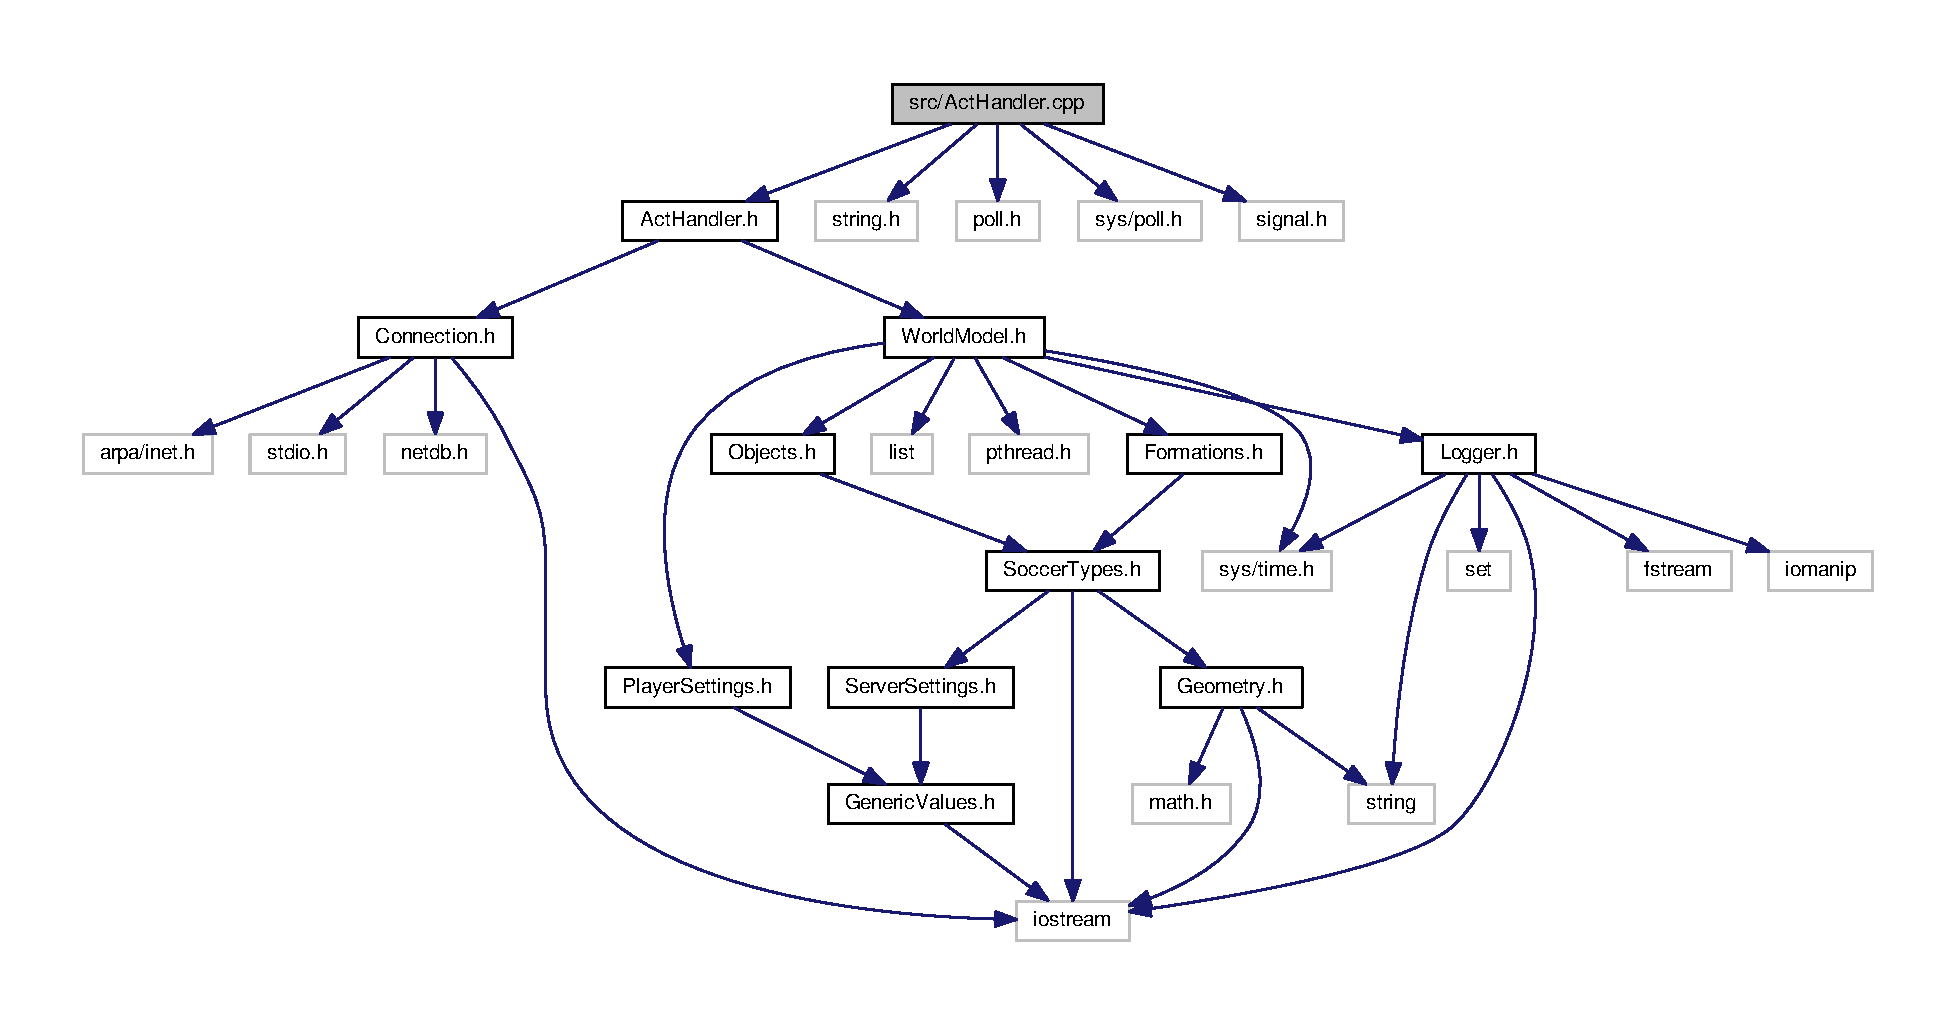
\includegraphics[width=350pt]{ActHandler_8cpp__incl}
\end{center}
\end{figure}
\subsection*{Functions}
\begin{DoxyCompactItemize}
\item 
void \hyperlink{ActHandler_8cpp_a5e8e3eb01478c3644f810f1a860e6499}{sigalarm\+Handler} (int i)
\end{DoxyCompactItemize}
\subsection*{Variables}
\begin{DoxyCompactItemize}
\item 
\hyperlink{classActHandler}{Act\+Handler} $\ast$ \hyperlink{ActHandler_8cpp_a25eb9052e6c6df32ebe5b29411d5c923}{A\+CT}
\end{DoxyCompactItemize}


\subsection{Detailed Description}

\begin{DoxyPre}
{\bfseries File:}          \hyperlink{ActHandler_8cpp}{ActHandler.cpp}
{\bfseries Project:}       Robocup Soccer Simulation Team: UvA Trilearn
{\bfseries Authors:}       Jelle Kok
{\bfseries Created:}       28/11/2000
{\bfseries Last Revision:} $ID\$
{\bfseries Contents:}      This file contains the class definitions for the
               \hyperlink{classActHandler}{ActHandler} that handles the outgoing messages to the
               server.



\subsubsection*{{\bfseries Changes}}\end{DoxyPre}



\begin{DoxyPre}
{\bfseries Date}             {\bfseries Author}          {\bfseries Comment}
28/11/2000       Jelle Kok       Initial version created
\end{DoxyPre}
 

\subsection{Function Documentation}
\index{Act\+Handler.\+cpp@{Act\+Handler.\+cpp}!sigalarm\+Handler@{sigalarm\+Handler}}
\index{sigalarm\+Handler@{sigalarm\+Handler}!Act\+Handler.\+cpp@{Act\+Handler.\+cpp}}
\subsubsection[{\texorpdfstring{sigalarm\+Handler(int i)}{sigalarmHandler(int i)}}]{\setlength{\rightskip}{0pt plus 5cm}void sigalarm\+Handler (
\begin{DoxyParamCaption}
\item[{int}]{i}
\end{DoxyParamCaption}
)}\hypertarget{ActHandler_8cpp_a5e8e3eb01478c3644f810f1a860e6499}{}\label{ActHandler_8cpp_a5e8e3eb01478c3644f810f1a860e6499}
This function is executed when a S\+I\+G\+A\+L\+A\+RM singal arrives. The time this signal comes is defined by the \hyperlink{classSenseHandler}{Sense\+Handler} (depending on incoming sense\+\_\+body messages). When the signal arrives, the commands currently stored in the queue of the \hyperlink{classActHandler}{Act\+Handler} are send to the server (using the method send\+Commands). 
\begin{DoxyParams}{Parameters}
{\em i} & is ignored \\
\hline
\end{DoxyParams}


\subsection{Variable Documentation}
\index{Act\+Handler.\+cpp@{Act\+Handler.\+cpp}!A\+CT@{A\+CT}}
\index{A\+CT@{A\+CT}!Act\+Handler.\+cpp@{Act\+Handler.\+cpp}}
\subsubsection[{\texorpdfstring{A\+CT}{ACT}}]{\setlength{\rightskip}{0pt plus 5cm}{\bf Act\+Handler}$\ast$ A\+CT}\hypertarget{ActHandler_8cpp_a25eb9052e6c6df32ebe5b29411d5c923}{}\label{ActHandler_8cpp_a25eb9052e6c6df32ebe5b29411d5c923}
Pointer to \hyperlink{classActHandler}{Act\+Handler} class needed by signal handler 
\hypertarget{ActHandler_8h}{}\section{src/\+Act\+Handler.h File Reference}
\label{ActHandler_8h}\index{src/\+Act\+Handler.\+h@{src/\+Act\+Handler.\+h}}
{\ttfamily \#include \char`\"{}Connection.\+h\char`\"{}}\\*
{\ttfamily \#include \char`\"{}World\+Model.\+h\char`\"{}}\\*
Include dependency graph for Act\+Handler.\+h\+:
\nopagebreak
\begin{figure}[H]
\begin{center}
\leavevmode
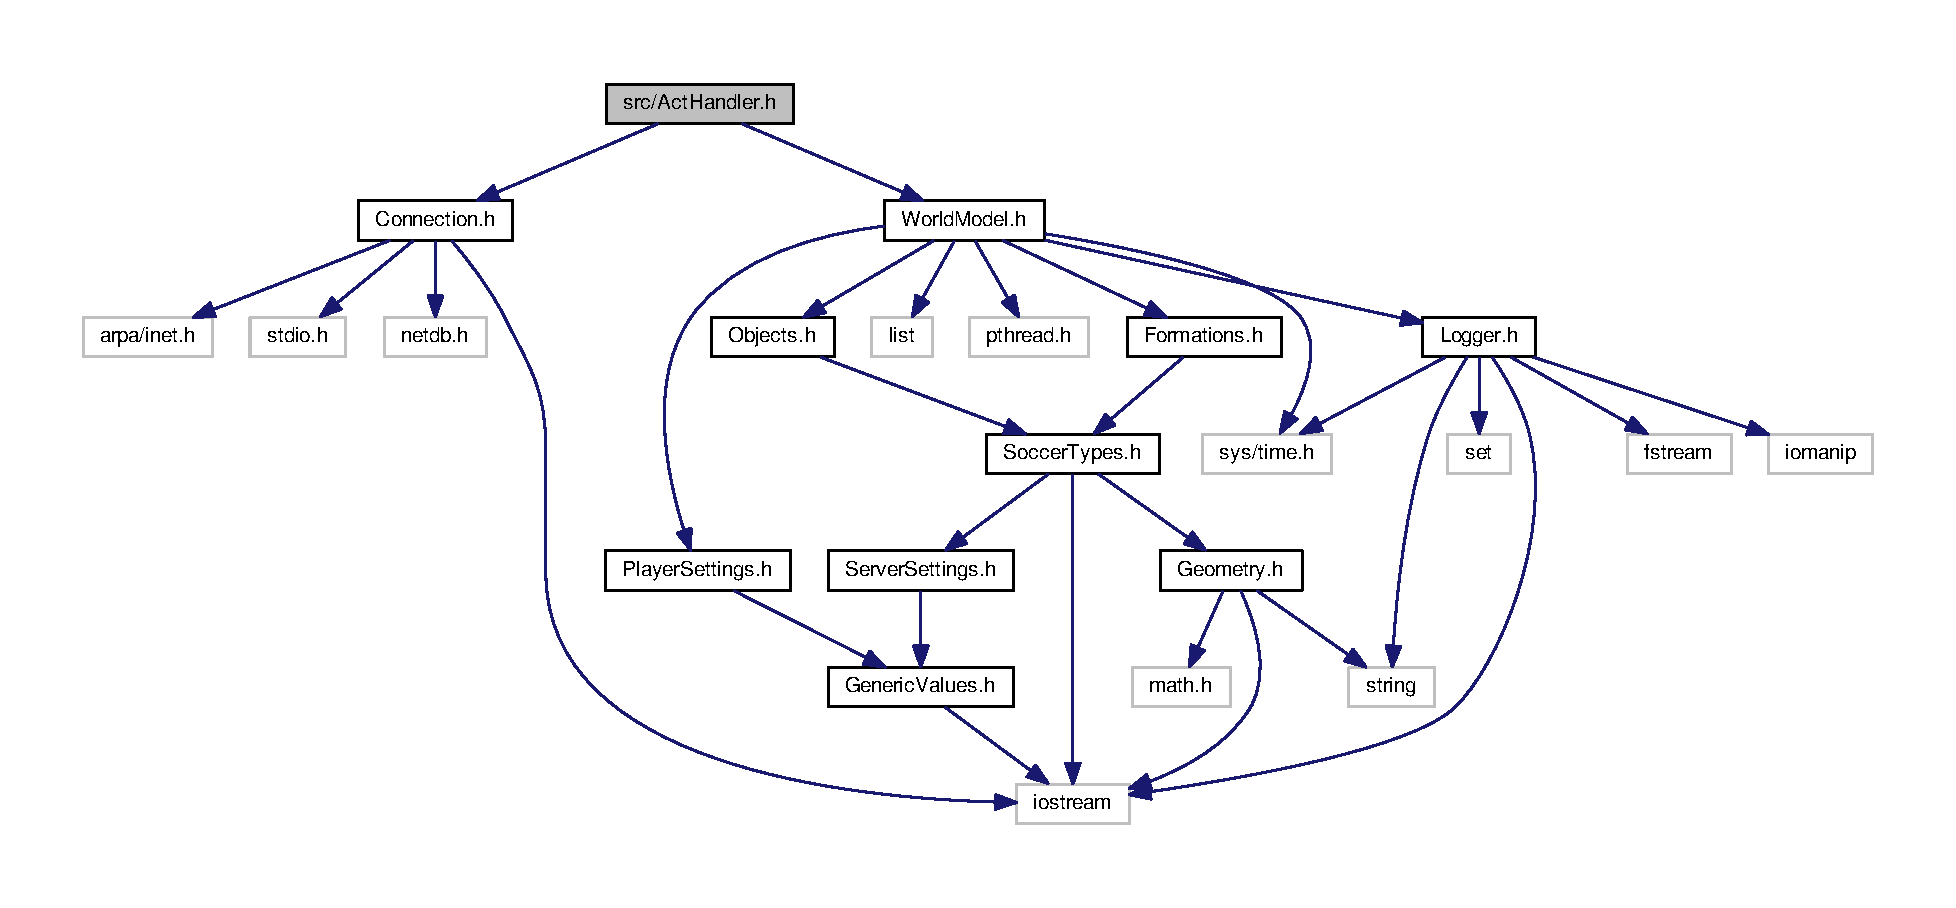
\includegraphics[width=350pt]{ActHandler_8h__incl}
\end{center}
\end{figure}
This graph shows which files directly or indirectly include this file\+:
\nopagebreak
\begin{figure}[H]
\begin{center}
\leavevmode
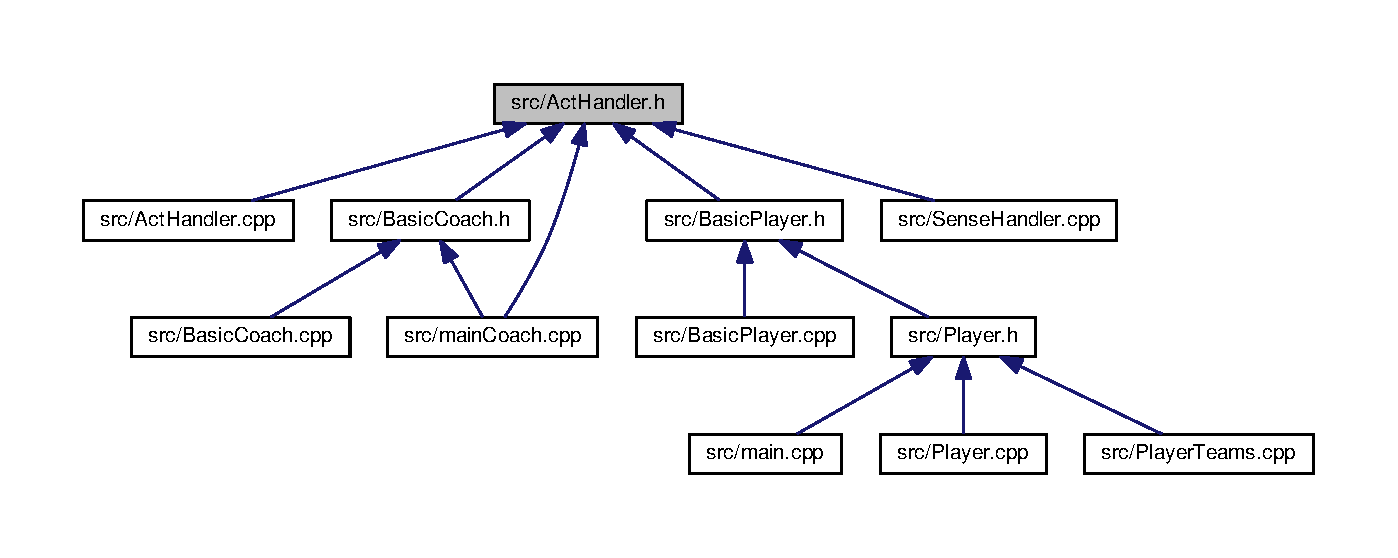
\includegraphics[width=350pt]{ActHandler_8h__dep__incl}
\end{center}
\end{figure}
\subsection*{Classes}
\begin{DoxyCompactItemize}
\item 
class \hyperlink{classActHandler}{Act\+Handler}
\end{DoxyCompactItemize}
\subsection*{Functions}
\begin{DoxyCompactItemize}
\item 
void \hyperlink{ActHandler_8h_a5e8e3eb01478c3644f810f1a860e6499}{sigalarm\+Handler} (int i)
\item 
void {\bfseries send\+Change\+View\+Commands} (int i\+Sync\+Counter)\hypertarget{ActHandler_8h_aa34cbff16cbe9015905b66cf9e04f2a4}{}\label{ActHandler_8h_aa34cbff16cbe9015905b66cf9e04f2a4}

\end{DoxyCompactItemize}
\subsection*{Variables}
\begin{DoxyCompactItemize}
\item 
\hyperlink{classLogger}{Logger} \hyperlink{ActHandler_8h_af2ed886ec3d2b2fd42fd0c5dad2f8cc5}{Log}
\end{DoxyCompactItemize}


\subsection{Detailed Description}

\begin{DoxyPre}
{\bfseries File:}          \hyperlink{ActHandler_8h}{ActHandler.h}
{\bfseries Project:}       Robocup Soccer Simulation Team: UvA Trilearn
{\bfseries Authors:}       Jelle Kok
{\bfseries Created:}       28/11/2000
{\bfseries Last Revision:} $ID\$
{\bfseries Contents:}      This file contains the class declarations for the
               \hyperlink{classActHandler}{ActHandler} that handles the outgoing messages to the
               server.



\subsubsection*{{\bfseries Changes}}\end{DoxyPre}



\begin{DoxyPre}
{\bfseries Date}             {\bfseries Author}          {\bfseries Comment}
28/11/2000       Jelle Kok       Initial version created
\end{DoxyPre}
 

\subsection{Function Documentation}
\index{Act\+Handler.\+h@{Act\+Handler.\+h}!sigalarm\+Handler@{sigalarm\+Handler}}
\index{sigalarm\+Handler@{sigalarm\+Handler}!Act\+Handler.\+h@{Act\+Handler.\+h}}
\subsubsection[{\texorpdfstring{sigalarm\+Handler(int i)}{sigalarmHandler(int i)}}]{\setlength{\rightskip}{0pt plus 5cm}void sigalarm\+Handler (
\begin{DoxyParamCaption}
\item[{int}]{i}
\end{DoxyParamCaption}
)}\hypertarget{ActHandler_8h_a5e8e3eb01478c3644f810f1a860e6499}{}\label{ActHandler_8h_a5e8e3eb01478c3644f810f1a860e6499}
This function is executed when a S\+I\+G\+A\+L\+A\+RM singal arrives. The time this signal comes is defined by the \hyperlink{classSenseHandler}{Sense\+Handler} (depending on incoming sense\+\_\+body messages). When the signal arrives, the commands currently stored in the queue of the \hyperlink{classActHandler}{Act\+Handler} are send to the server (using the method send\+Commands). 
\begin{DoxyParams}{Parameters}
{\em i} & is ignored \\
\hline
\end{DoxyParams}


\subsection{Variable Documentation}
\index{Act\+Handler.\+h@{Act\+Handler.\+h}!Log@{Log}}
\index{Log@{Log}!Act\+Handler.\+h@{Act\+Handler.\+h}}
\subsubsection[{\texorpdfstring{Log}{Log}}]{\setlength{\rightskip}{0pt plus 5cm}{\bf Logger} Log}\hypertarget{ActHandler_8h_af2ed886ec3d2b2fd42fd0c5dad2f8cc5}{}\label{ActHandler_8h_af2ed886ec3d2b2fd42fd0c5dad2f8cc5}
Reference to the \hyperlink{classLogger}{Logger} to write log info to

\hyperlink{classLogger}{Logger} instantation that can be used by all classes 
\hypertarget{BasicCoach_8cpp}{}\section{src/\+Basic\+Coach.cpp File Reference}
\label{BasicCoach_8cpp}\index{src/\+Basic\+Coach.\+cpp@{src/\+Basic\+Coach.\+cpp}}
{\ttfamily \#include \char`\"{}Basic\+Coach.\+h\char`\"{}}\\*
{\ttfamily \#include \char`\"{}Parse.\+h\char`\"{}}\\*
{\ttfamily \#include $<$sys/poll.\+h$>$}\\*
Include dependency graph for Basic\+Coach.\+cpp\+:
\nopagebreak
\begin{figure}[H]
\begin{center}
\leavevmode
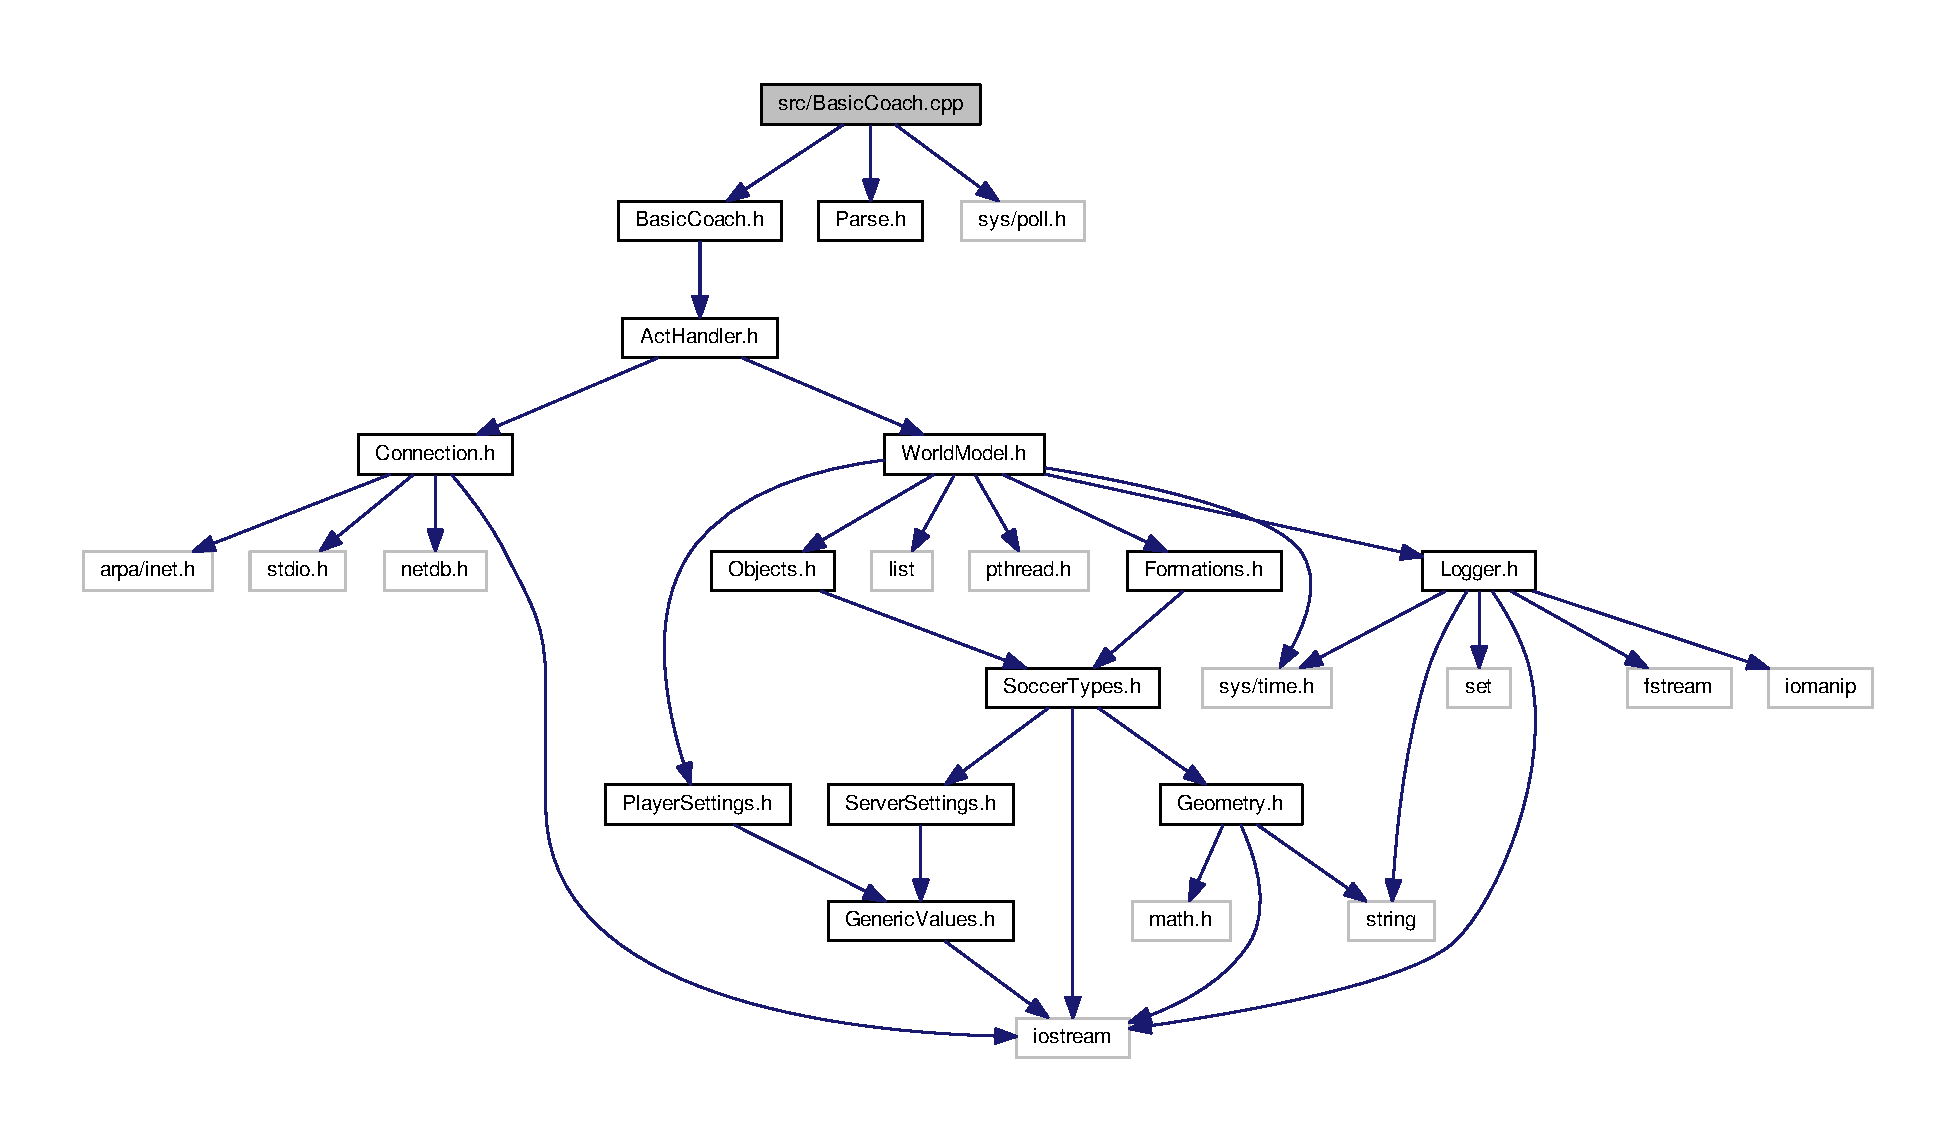
\includegraphics[width=350pt]{BasicCoach_8cpp__incl}
\end{center}
\end{figure}
\subsection*{Functions}
\begin{DoxyCompactItemize}
\item 
void $\ast$ {\bfseries stdin\+\_\+callback} (void $\ast$v)\hypertarget{BasicCoach_8cpp_a61ef2ff77d560bee258e79ccc69598d7}{}\label{BasicCoach_8cpp_a61ef2ff77d560bee258e79ccc69598d7}

\end{DoxyCompactItemize}
\subsection*{Variables}
\begin{DoxyCompactItemize}
\item 
\hyperlink{classLogger}{Logger} \hyperlink{BasicCoach_8cpp_af2ed886ec3d2b2fd42fd0c5dad2f8cc5}{Log}
\end{DoxyCompactItemize}


\subsection{Detailed Description}

\begin{DoxyPre}
{\bfseries File:}          \hyperlink{BasicCoach_8cpp}{BasicCoach.cpp}
{\bfseries Project:}       Robocup Soccer Simulation Team: UvA Trilearn
{\bfseries Authors:}       Jelle Kok
{\bfseries Created:}       03/03/2001
{\bfseries Last Revision:} $ID\$
{\bfseries Contents:}      This file contains the class definitions for the
                      \hyperlink{classBasicCoach}{BasicCoach} which contains the main structure for the 
                      coach.



\subsubsection*{{\bfseries Changes}}\end{DoxyPre}



\begin{DoxyPre}
{\bfseries Date}             {\bfseries Author}          {\bfseries Comment}
03/03/2001        Jelle Kok       Initial version created
\end{DoxyPre}
 

\subsection{Variable Documentation}
\index{Basic\+Coach.\+cpp@{Basic\+Coach.\+cpp}!Log@{Log}}
\index{Log@{Log}!Basic\+Coach.\+cpp@{Basic\+Coach.\+cpp}}
\subsubsection[{\texorpdfstring{Log}{Log}}]{\setlength{\rightskip}{0pt plus 5cm}{\bf Logger} Log}\hypertarget{BasicCoach_8cpp_af2ed886ec3d2b2fd42fd0c5dad2f8cc5}{}\label{BasicCoach_8cpp_af2ed886ec3d2b2fd42fd0c5dad2f8cc5}
This is a reference to the \hyperlink{classLogger}{Logger} to write loginfo to

\hyperlink{classLogger}{Logger} instantation that can be used by all classes 
\hypertarget{BasicCoach_8h}{}\section{src/\+Basic\+Coach.h File Reference}
\label{BasicCoach_8h}\index{src/\+Basic\+Coach.\+h@{src/\+Basic\+Coach.\+h}}
{\ttfamily \#include \char`\"{}Act\+Handler.\+h\char`\"{}}\\*
Include dependency graph for Basic\+Coach.\+h\+:
\nopagebreak
\begin{figure}[H]
\begin{center}
\leavevmode
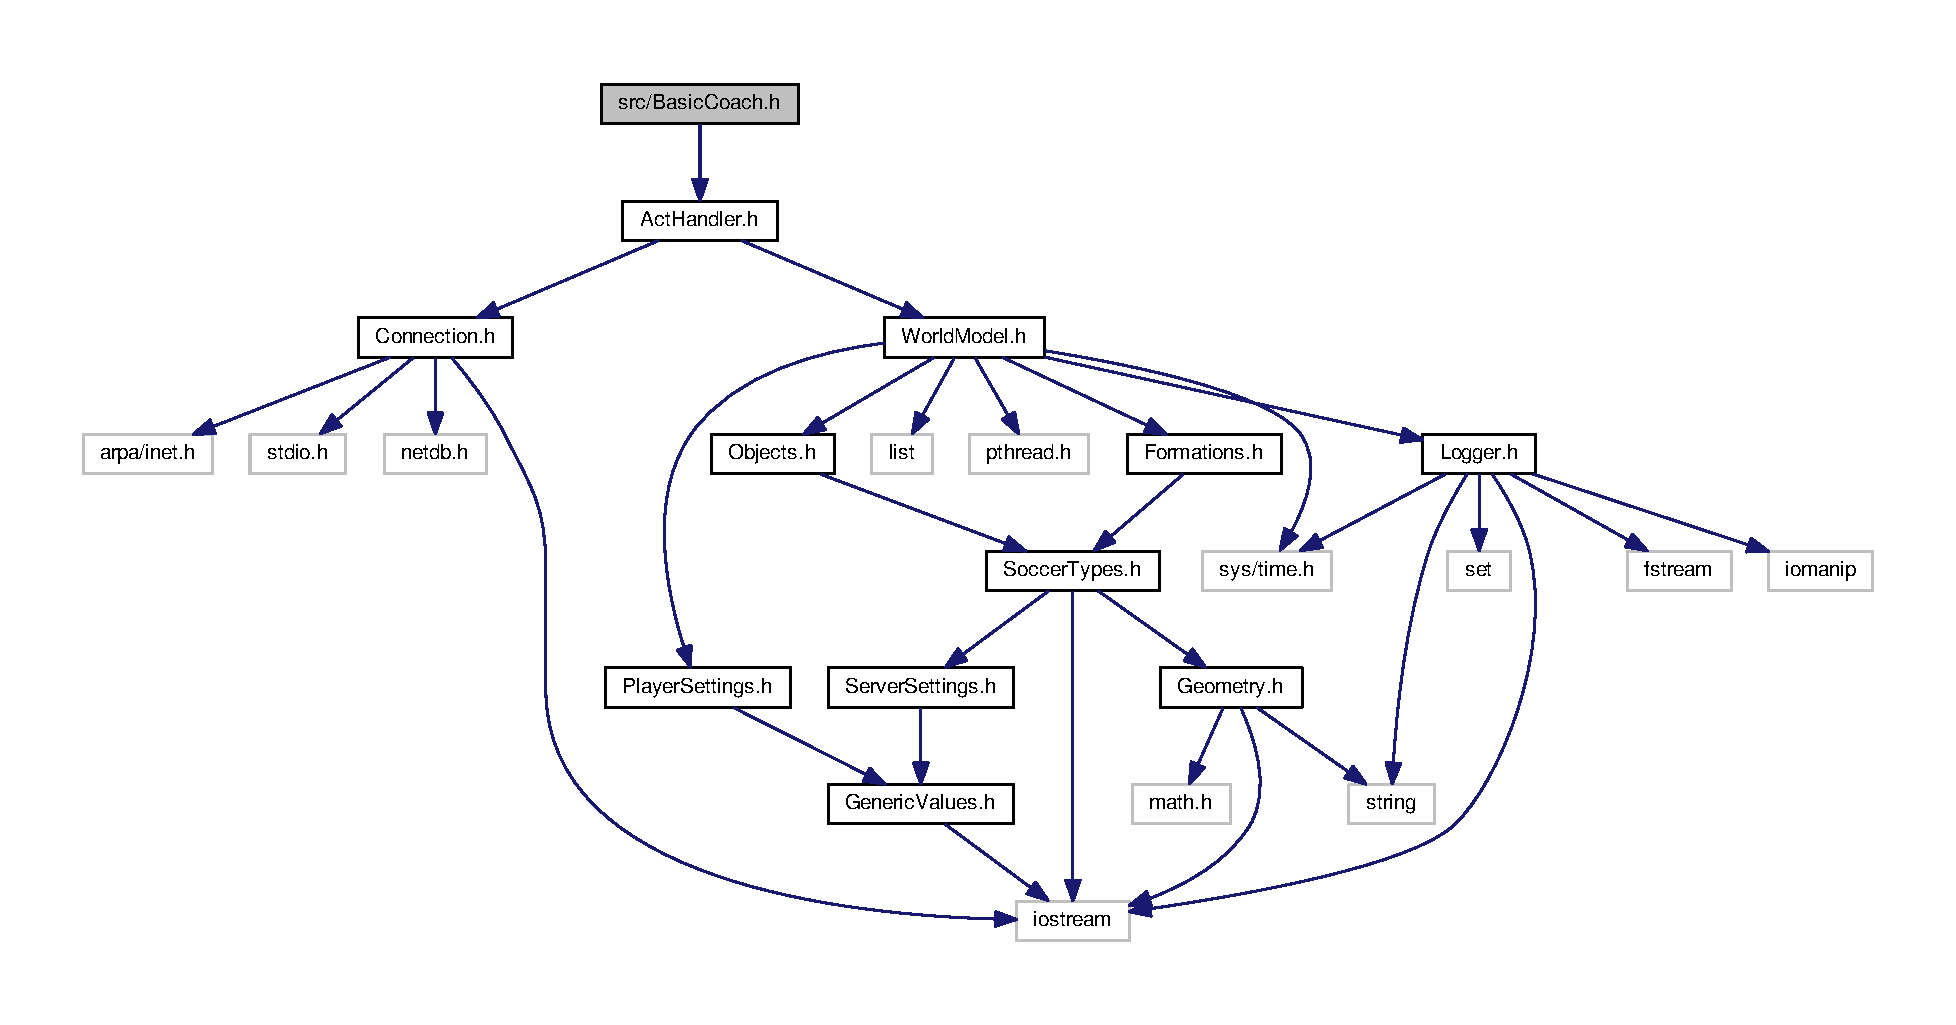
\includegraphics[width=350pt]{BasicCoach_8h__incl}
\end{center}
\end{figure}
This graph shows which files directly or indirectly include this file\+:
\nopagebreak
\begin{figure}[H]
\begin{center}
\leavevmode
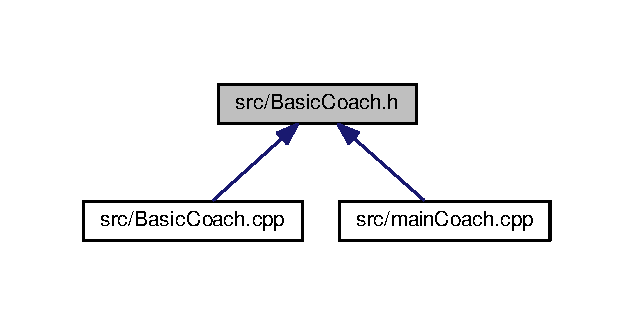
\includegraphics[width=304pt]{BasicCoach_8h__dep__incl}
\end{center}
\end{figure}
\subsection*{Classes}
\begin{DoxyCompactItemize}
\item 
class \hyperlink{classBasicCoach}{Basic\+Coach}
\end{DoxyCompactItemize}
\subsection*{Functions}
\begin{DoxyCompactItemize}
\item 
void $\ast$ \hyperlink{BasicCoach_8h_a61ef2ff77d560bee258e79ccc69598d7}{stdin\+\_\+callback} (void $\ast$v)
\end{DoxyCompactItemize}


\subsection{Detailed Description}

\begin{DoxyPre}
{\bfseries File:}          \hyperlink{BasicCoach_8h}{BasicCoach.h}
{\bfseries Project:}       Robocup Soccer Simulation Team: UvA Trilearn
{\bfseries Authors:}       Jelle Kok
{\bfseries Created:}       03/03/2001
{\bfseries Last Revision:} $ID\$
{\bfseries Contents:}      This file contains the class declarations for the
                      \hyperlink{classBasicCoach}{BasicCoach} which contains the main structure for the 
                      case.



\subsubsection*{{\bfseries Changes}}\end{DoxyPre}



\begin{DoxyPre}
{\bfseries Date}             {\bfseries Author}          {\bfseries Comment}
03/03/2001        Jelle Kok       Initial version created
\end{DoxyPre}
 

\subsection{Function Documentation}
\index{Basic\+Coach.\+h@{Basic\+Coach.\+h}!stdin\+\_\+callback@{stdin\+\_\+callback}}
\index{stdin\+\_\+callback@{stdin\+\_\+callback}!Basic\+Coach.\+h@{Basic\+Coach.\+h}}
\subsubsection[{\texorpdfstring{stdin\+\_\+callback(void $\ast$v)}{stdin_callback(void *v)}}]{\setlength{\rightskip}{0pt plus 5cm}void$\ast$ stdin\+\_\+callback (
\begin{DoxyParamCaption}
\item[{void $\ast$}]{v}
\end{DoxyParamCaption}
)}\hypertarget{BasicCoach_8h_a61ef2ff77d560bee258e79ccc69598d7}{}\label{BasicCoach_8h_a61ef2ff77d560bee258e79ccc69598d7}
This method can be called in a separate thread (see pthread\+\_\+create) since it returns a void pointer. It is assumed that this function receives a \hyperlink{classBasicPlayer}{Basic\+Player} class as argument. The only thing this function does is starting the method handle\+Stdin() from the corresponding \hyperlink{classBasicPlayer}{Basic\+Player} class that listens to user input from the keyboard. This function is necessary since a method from a class cannot be an argument of pthread\+\_\+create. 
\begin{DoxyParams}{Parameters}
{\em v} & void pointer to a \hyperlink{classBasicPlayer}{Basic\+Player} class. \\
\hline
\end{DoxyParams}
\begin{DoxyReturn}{Returns}
should never return since function handle\+Stdin has infinite loop 
\end{DoxyReturn}

\hypertarget{BasicPlayer_8cpp}{}\section{src/\+Basic\+Player.cpp File Reference}
\label{BasicPlayer_8cpp}\index{src/\+Basic\+Player.\+cpp@{src/\+Basic\+Player.\+cpp}}
{\ttfamily \#include \char`\"{}Basic\+Player.\+h\char`\"{}}\\*
{\ttfamily \#include \char`\"{}Parse.\+h\char`\"{}}\\*
Include dependency graph for Basic\+Player.\+cpp\+:
\nopagebreak
\begin{figure}[H]
\begin{center}
\leavevmode
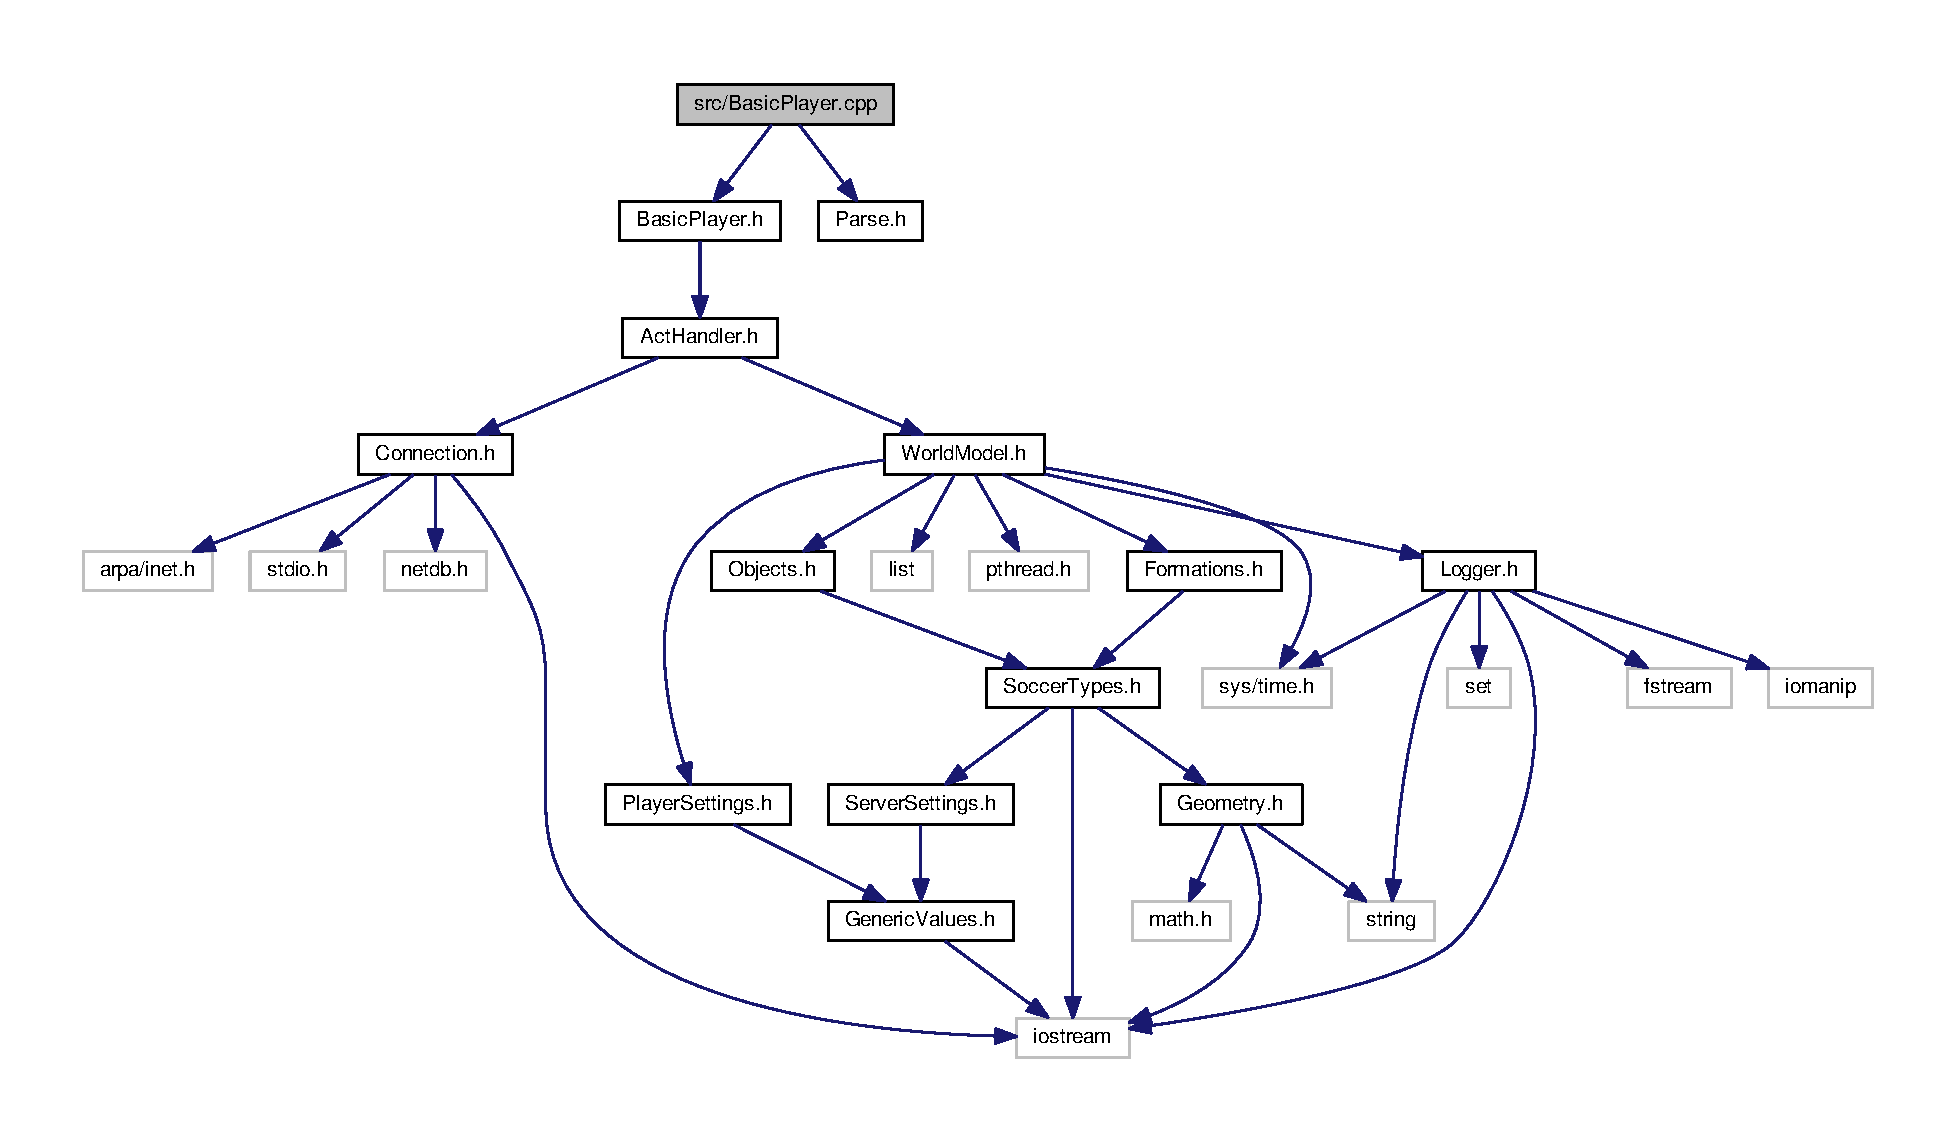
\includegraphics[width=350pt]{BasicPlayer_8cpp__incl}
\end{center}
\end{figure}


\subsection{Detailed Description}

\begin{DoxyPre}
{\bfseries File:}          \hyperlink{BasicPlayer_8cpp}{BasicPlayer.cpp}
{\bfseries Project:}       Robocup Soccer Simulation Team: UvA Trilearn
{\bfseries Authors:}       Jelle Kok
{\bfseries Created:}       10/12/2000
{\bfseries Last Revision:} $ID\$
{\bfseries Contents:}      This file contains the class declaration for the
               \hyperlink{classBasicPlayer}{BasicPlayer}. The \hyperlink{classBasicPlayer}{BasicPlayer} is the class where the
               available skills for the agent are defined.



\subsubsection*{{\bfseries Changes}}\end{DoxyPre}



\begin{DoxyPre}
{\bfseries Date}             {\bfseries Author}          {\bfseries Comment}:
10/12/2000       Jelle Kok       Initial version created
\end{DoxyPre}
 
\hypertarget{BasicPlayer_8h}{}\section{src/\+Basic\+Player.h File Reference}
\label{BasicPlayer_8h}\index{src/\+Basic\+Player.\+h@{src/\+Basic\+Player.\+h}}
{\ttfamily \#include \char`\"{}Act\+Handler.\+h\char`\"{}}\\*
Include dependency graph for Basic\+Player.\+h\+:
\nopagebreak
\begin{figure}[H]
\begin{center}
\leavevmode
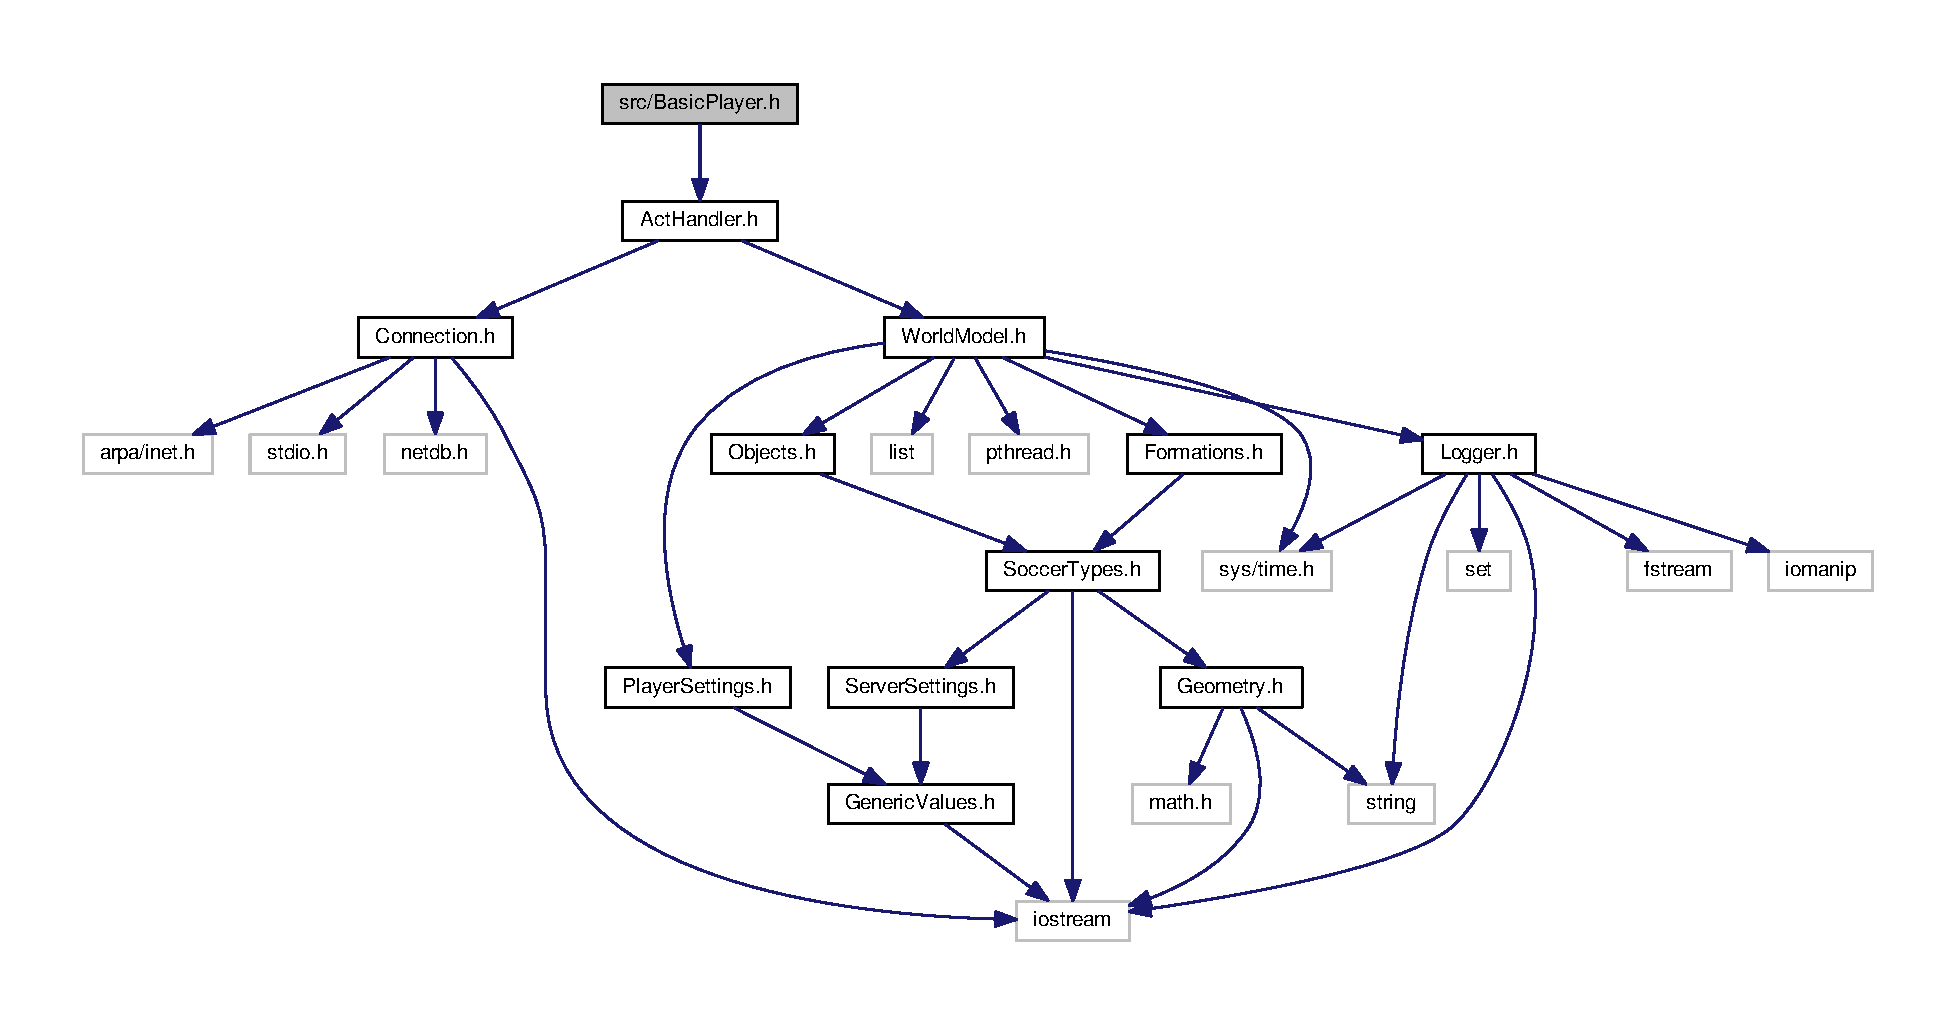
\includegraphics[width=350pt]{BasicPlayer_8h__incl}
\end{center}
\end{figure}
This graph shows which files directly or indirectly include this file\+:
\nopagebreak
\begin{figure}[H]
\begin{center}
\leavevmode
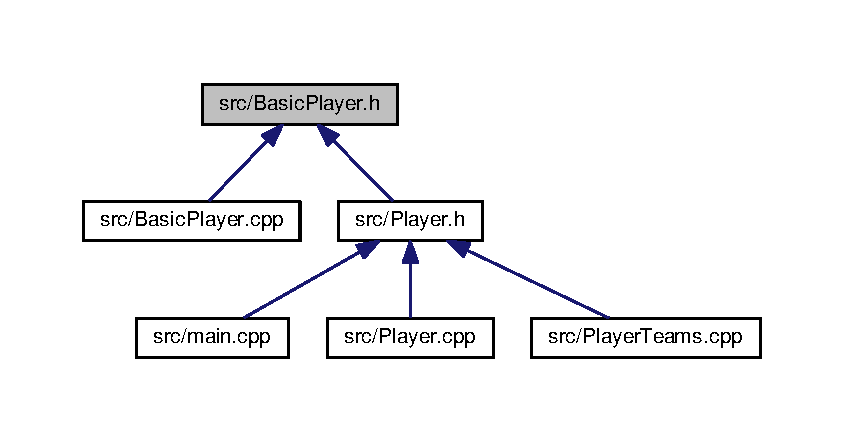
\includegraphics[width=350pt]{BasicPlayer_8h__dep__incl}
\end{center}
\end{figure}
\subsection*{Classes}
\begin{DoxyCompactItemize}
\item 
class \hyperlink{classBasicPlayer}{Basic\+Player}
\end{DoxyCompactItemize}
\subsection*{Variables}
\begin{DoxyCompactItemize}
\item 
\hyperlink{classLogger}{Logger} \hyperlink{BasicPlayer_8h_af2ed886ec3d2b2fd42fd0c5dad2f8cc5}{Log}
\end{DoxyCompactItemize}


\subsection{Detailed Description}

\begin{DoxyPre}
{\bfseries File:}          \hyperlink{BasicPlayer_8h}{BasicPlayer.h}
{\bfseries Project:}       Robocup Soccer Simulation Team: UvA Trilearn
{\bfseries Authors:}       Jelle Kok
{\bfseries Created:}       10/12/2000
{\bfseries Last Revision:} $ID\$
{\bfseries Contents:}      This file contains the class definitions for the
               \hyperlink{classBasicPlayer}{BasicPlayer}. The \hyperlink{classBasicPlayer}{BasicPlayer} is the class where the
               available skills for the agent are defined.



\subsubsection*{{\bfseries Changes}}\end{DoxyPre}



\begin{DoxyPre}
{\bfseries Date}             {\bfseries Author}          {\bfseries Comment}
10/12/2000       Jelle Kok       Initial version created
\end{DoxyPre}
 

\subsection{Variable Documentation}
\index{Basic\+Player.\+h@{Basic\+Player.\+h}!Log@{Log}}
\index{Log@{Log}!Basic\+Player.\+h@{Basic\+Player.\+h}}
\subsubsection[{\texorpdfstring{Log}{Log}}]{\setlength{\rightskip}{0pt plus 5cm}{\bf Logger} Log}\hypertarget{BasicPlayer_8h_af2ed886ec3d2b2fd42fd0c5dad2f8cc5}{}\label{BasicPlayer_8h_af2ed886ec3d2b2fd42fd0c5dad2f8cc5}
This is a reference to \hyperlink{classLogger}{Logger} to write log info to

\hyperlink{classLogger}{Logger} instantation that can be used by all classes 
\hypertarget{Connection_8cpp}{}\section{src/\+Connection.cpp File Reference}
\label{Connection_8cpp}\index{src/\+Connection.\+cpp@{src/\+Connection.\+cpp}}
{\ttfamily \#include $<$errno.\+h$>$}\\*
{\ttfamily \#include $<$string.\+h$>$}\\*
{\ttfamily \#include $<$sys/types.\+h$>$}\\*
{\ttfamily \#include $<$unistd.\+h$>$}\\*
{\ttfamily \#include $<$sys/socket.\+h$>$}\\*
{\ttfamily \#include \char`\"{}Connection.\+h\char`\"{}}\\*
{\ttfamily \#include \char`\"{}Logger.\+h\char`\"{}}\\*
Include dependency graph for Connection.\+cpp\+:
\nopagebreak
\begin{figure}[H]
\begin{center}
\leavevmode
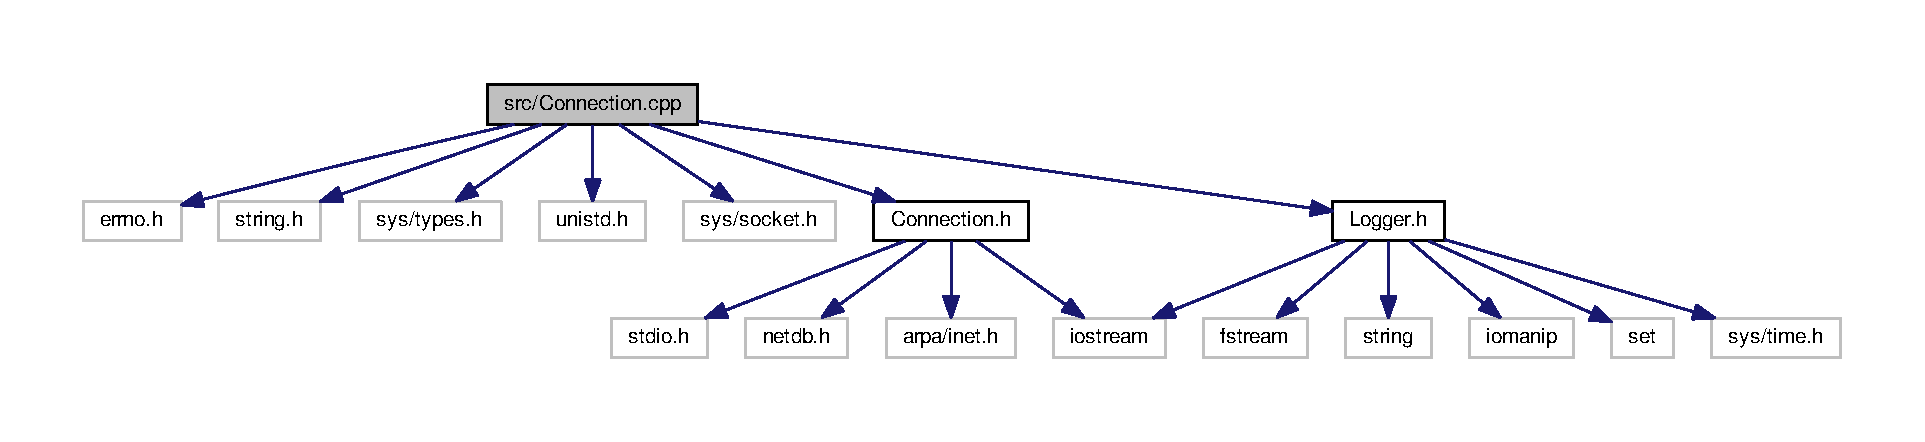
\includegraphics[width=350pt]{Connection_8cpp__incl}
\end{center}
\end{figure}
\subsection*{Variables}
\begin{DoxyCompactItemize}
\item 
\hyperlink{classLogger}{Logger} \hyperlink{Connection_8cpp_af2ed886ec3d2b2fd42fd0c5dad2f8cc5}{Log}
\end{DoxyCompactItemize}


\subsection{Detailed Description}

\begin{DoxyPre}
{\bfseries File:}          \hyperlink{Connection_8cpp}{Connection.cpp}
{\bfseries Project:}       Robocup Soccer Simulation Team: UvA Trilearn
{\bfseries Authors:}       Jelle Kok
{\bfseries Created:}       23/11/2000
{\bfseries Last Revision:} $ID\$
{\bfseries Contents:}      This file contains the class definitions for the
               \hyperlink{classConnection}{Connection} class which sets up a connection with the
               soccer server.



\subsubsection*{{\bfseries Changes}}\end{DoxyPre}



\begin{DoxyPre}
{\bfseries Date}             {\bfseries Author}          {\bfseries Comment}
23/11/2000       Jelle Kok       Initial version created
\end{DoxyPre}
 

\subsection{Variable Documentation}
\index{Connection.\+cpp@{Connection.\+cpp}!Log@{Log}}
\index{Log@{Log}!Connection.\+cpp@{Connection.\+cpp}}
\subsubsection[{\texorpdfstring{Log}{Log}}]{\setlength{\rightskip}{0pt plus 5cm}{\bf Logger} Log}\hypertarget{Connection_8cpp_af2ed886ec3d2b2fd42fd0c5dad2f8cc5}{}\label{Connection_8cpp_af2ed886ec3d2b2fd42fd0c5dad2f8cc5}
This is a reference to the \hyperlink{classLogger}{Logger} for writing info to

\hyperlink{classLogger}{Logger} instantation that can be used by all classes 
\hypertarget{Connection_8h}{}\section{src/\+Connection.h File Reference}
\label{Connection_8h}\index{src/\+Connection.\+h@{src/\+Connection.\+h}}
{\ttfamily \#include $<$stdio.\+h$>$}\\*
{\ttfamily \#include $<$iostream$>$}\\*
{\ttfamily \#include $<$netdb.\+h$>$}\\*
{\ttfamily \#include $<$arpa/inet.\+h$>$}\\*
Include dependency graph for Connection.\+h\+:
\nopagebreak
\begin{figure}[H]
\begin{center}
\leavevmode
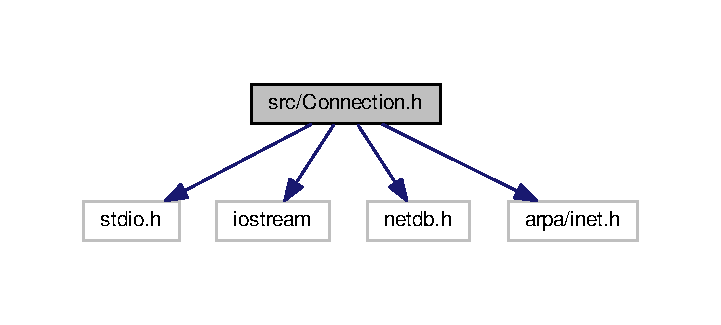
\includegraphics[width=346pt]{Connection_8h__incl}
\end{center}
\end{figure}
This graph shows which files directly or indirectly include this file\+:
\nopagebreak
\begin{figure}[H]
\begin{center}
\leavevmode
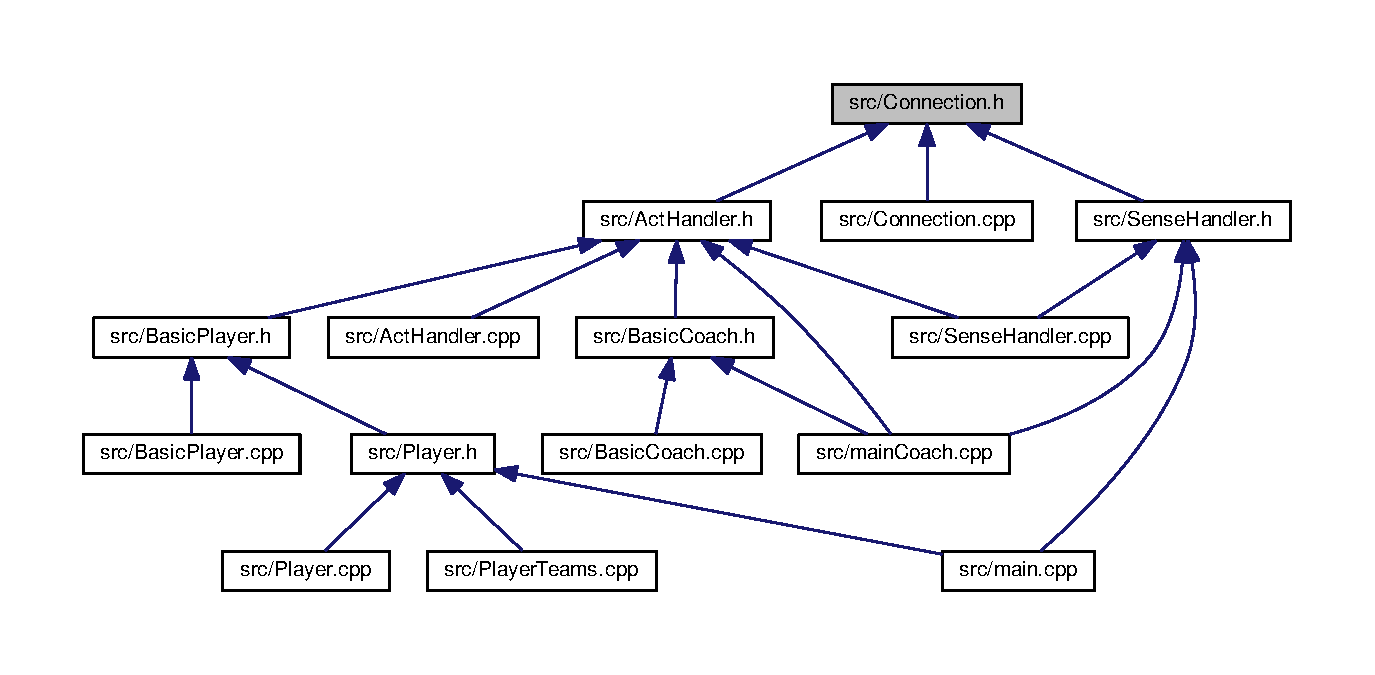
\includegraphics[width=350pt]{Connection_8h__dep__incl}
\end{center}
\end{figure}
\subsection*{Classes}
\begin{DoxyCompactItemize}
\item 
struct \hyperlink{struct__socket}{\+\_\+socket}
\item 
class \hyperlink{classConnection}{Connection}
\end{DoxyCompactItemize}
\subsection*{Typedefs}
\begin{DoxyCompactItemize}
\item 
typedef struct \hyperlink{struct__socket}{\+\_\+socket} \hyperlink{Connection_8h_a832868b6e6b0ffea4ff0f7c05aa0dee5}{Socket}
\end{DoxyCompactItemize}


\subsection{Detailed Description}

\begin{DoxyPre}
{\bfseries File:}          \hyperlink{Connection_8h}{Connection.h}
{\bfseries Project:}       Robocup Soccer Simulation Team: UvA Trilearn
{\bfseries Authors:}       Jelle Kok
{\bfseries Created:}       23/11/2000
{\bfseries Last Revision:} $ID\$
{\bfseries Contents:}      This file contains the class declarations for the
               \hyperlink{classConnection}{Connection} class which sets up a connection with the
               soccer server.



\subsubsection*{{\bfseries Changes}}\end{DoxyPre}



\begin{DoxyPre}
{\bfseries Date}             {\bfseries Author}          {\bfseries Comment}
23/11/2000      Jelle Kok       Initial version created
\end{DoxyPre}
 

\subsection{Typedef Documentation}
\index{Connection.\+h@{Connection.\+h}!Socket@{Socket}}
\index{Socket@{Socket}!Connection.\+h@{Connection.\+h}}
\subsubsection[{\texorpdfstring{Socket}{Socket}}]{\setlength{\rightskip}{0pt plus 5cm}typedef struct {\bf \+\_\+socket}  {\bf Socket}}\hypertarget{Connection_8h_a832868b6e6b0ffea4ff0f7c05aa0dee5}{}\label{Connection_8h_a832868b6e6b0ffea4ff0f7c05aa0dee5}
Socket is a combination of a filedescriptor with a server adress. 
\hypertarget{Formations_8cpp}{}\section{src/\+Formations.cpp File Reference}
\label{Formations_8cpp}\index{src/\+Formations.\+cpp@{src/\+Formations.\+cpp}}
{\ttfamily \#include \char`\"{}Formations.\+h\char`\"{}}\\*
{\ttfamily \#include \char`\"{}Parse.\+h\char`\"{}}\\*
{\ttfamily \#include $<$fstream$>$}\\*
{\ttfamily \#include $<$stdio.\+h$>$}\\*
{\ttfamily \#include $<$math.\+h$>$}\\*
Include dependency graph for Formations.\+cpp\+:
\nopagebreak
\begin{figure}[H]
\begin{center}
\leavevmode
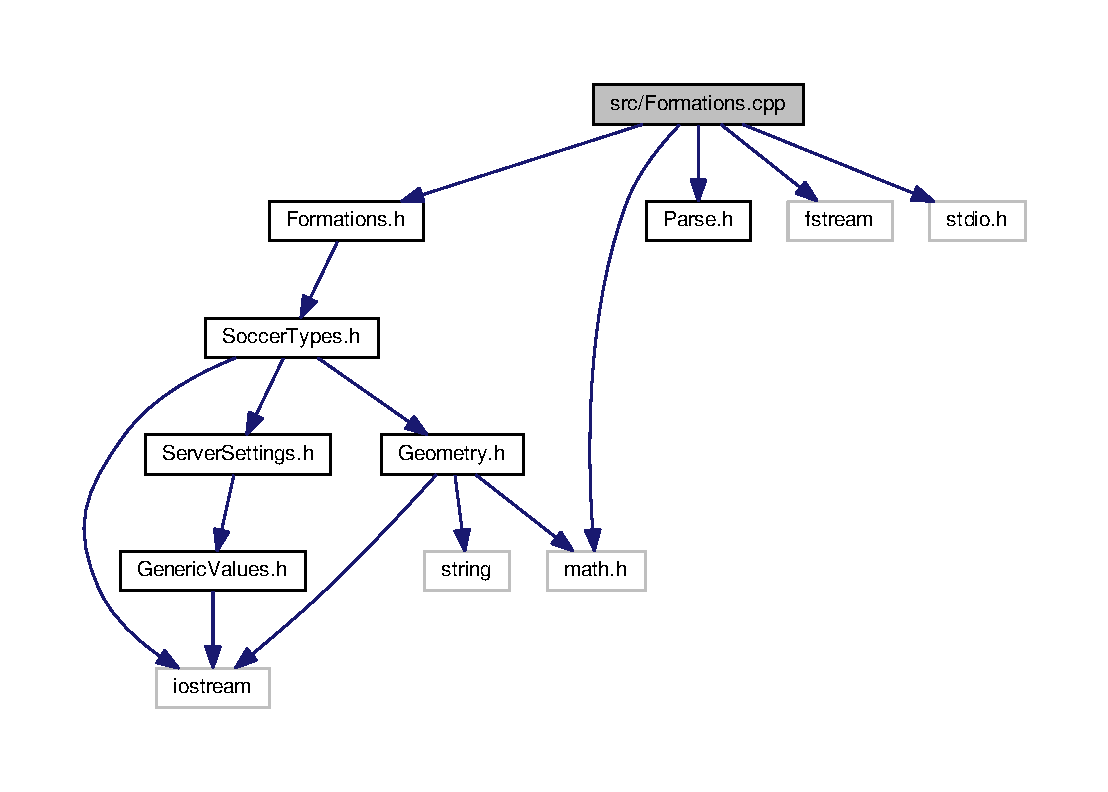
\includegraphics[width=350pt]{Formations_8cpp__incl}
\end{center}
\end{figure}


\subsection{Detailed Description}

\begin{DoxyPre}
{\bfseries File:}          \hyperlink{Formations_8cpp}{Formations.cpp}
{\bfseries Project:}       Robocup Soccer Simulation Team: UvA Trilearn
{\bfseries Authors:}       Jelle Kok
{\bfseries Created:}       05/02/2001
{\bfseries Last Revision:} $ID\$
{\bfseries Contents:}      Definitions for the different methods in the classes that
               are associated with \hyperlink{classFormations}{Formations}.                      .



\subsubsection*{{\bfseries Changes}}\end{DoxyPre}



\begin{DoxyPre}
{\bfseries Date}             {\bfseries Author}          {\bfseries Comment}
05/02/2001       Jelle Kok       Initial version created
\end{DoxyPre}
 
\hypertarget{Formations_8h}{}\section{src/\+Formations.h File Reference}
\label{Formations_8h}\index{src/\+Formations.\+h@{src/\+Formations.\+h}}
{\ttfamily \#include \char`\"{}Soccer\+Types.\+h\char`\"{}}\\*
Include dependency graph for Formations.\+h\+:
\nopagebreak
\begin{figure}[H]
\begin{center}
\leavevmode
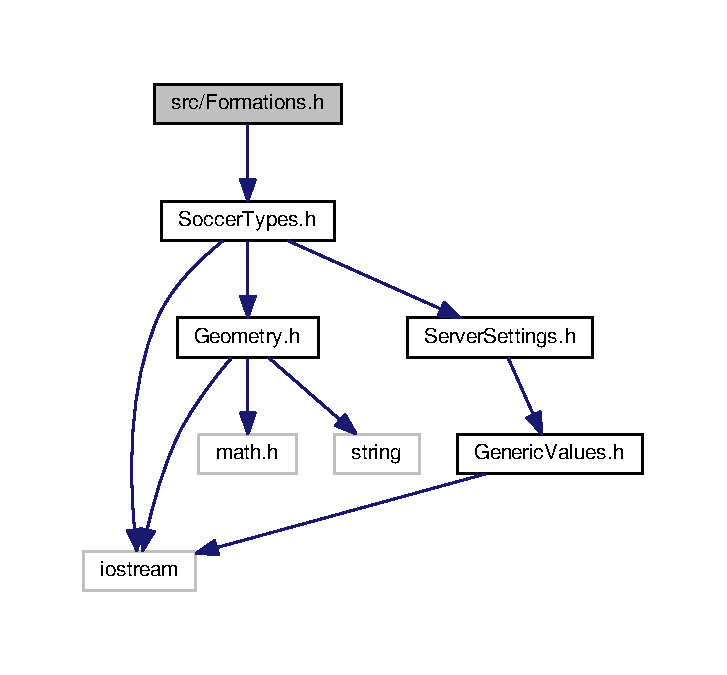
\includegraphics[width=349pt]{Formations_8h__incl}
\end{center}
\end{figure}
This graph shows which files directly or indirectly include this file\+:
\nopagebreak
\begin{figure}[H]
\begin{center}
\leavevmode
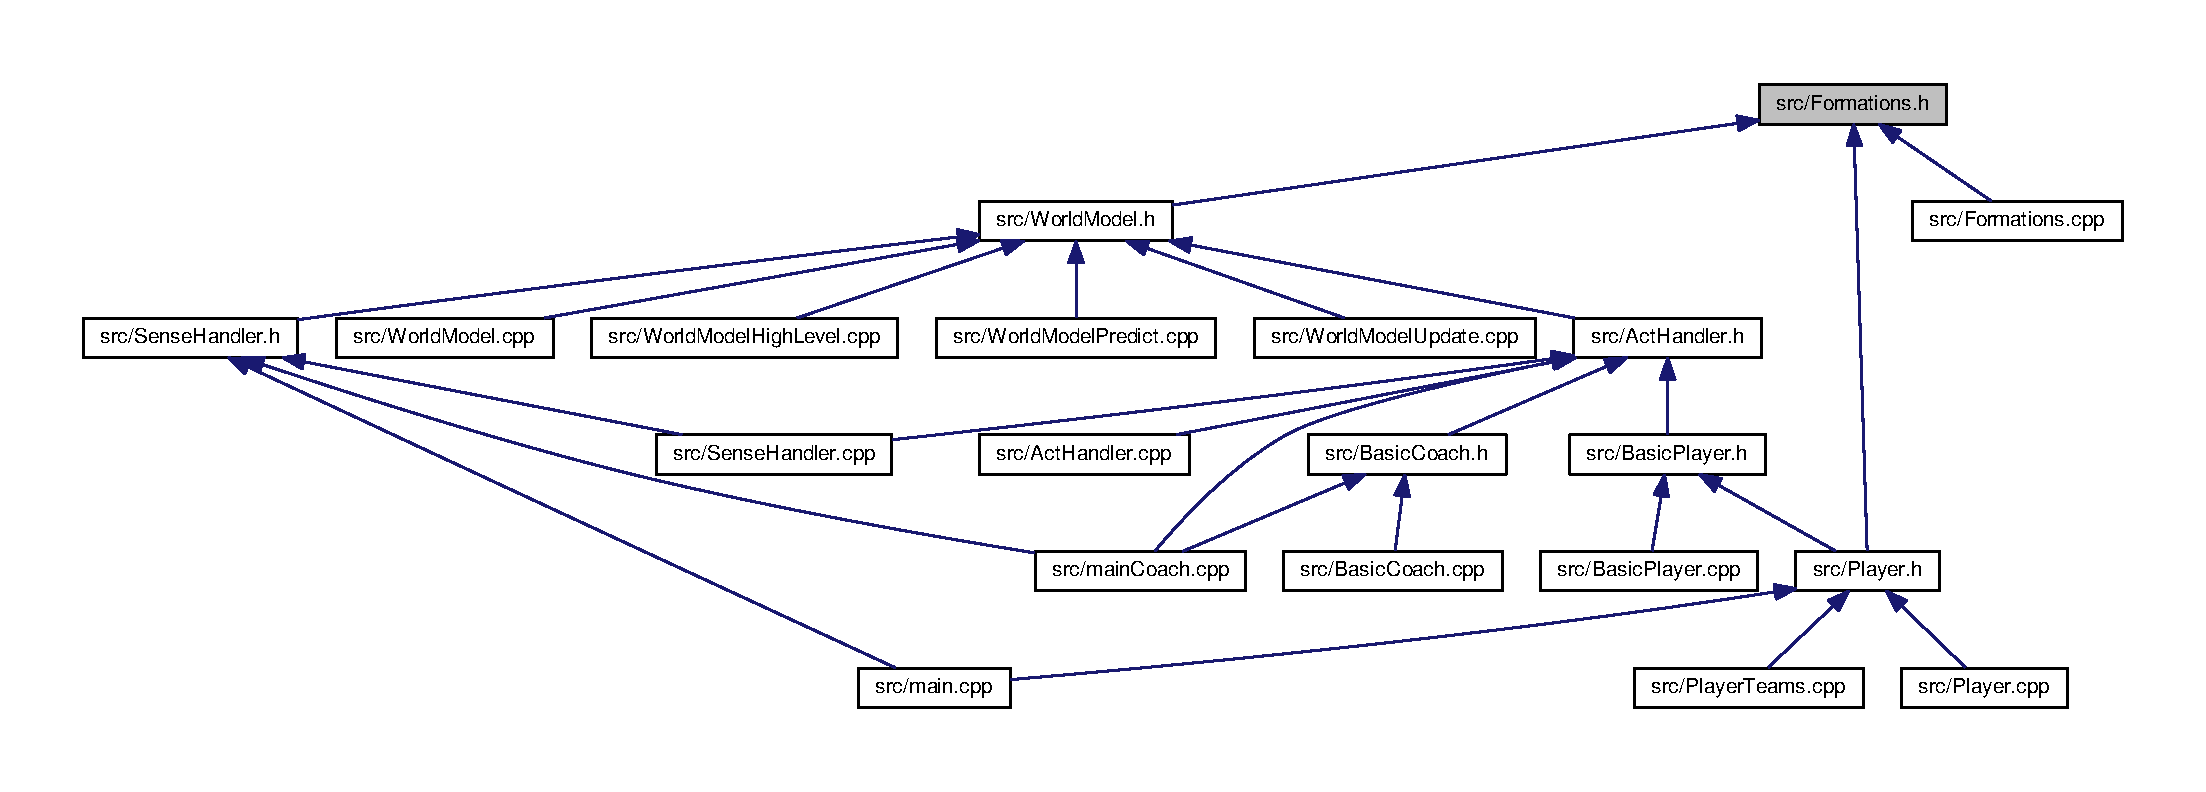
\includegraphics[width=350pt]{Formations_8h__dep__incl}
\end{center}
\end{figure}
\subsection*{Classes}
\begin{DoxyCompactItemize}
\item 
class \hyperlink{classPlayerTypeInfo}{Player\+Type\+Info}
\item 
class \hyperlink{classFormationTypeInfo}{Formation\+Type\+Info}
\item 
class \hyperlink{classFormations}{Formations}
\end{DoxyCompactItemize}


\subsection{Detailed Description}

\begin{DoxyPre}\end{DoxyPre}



\begin{DoxyPre}{\bfseries File:}          \hyperlink{Formations_8h}{Formations.h}
{\bfseries Project:}       Robocup Soccer Simulation Team: UvA Trilearn
{\bfseries Authors:}       Jelle Kok
{\bfseries Created:}       05/02/2001
{\bfseries Last Revision:} $ID\$
{\bfseries Contents:}      Header file for different classes associated with
               \hyperlink{classFormations}{Formations}.\end{DoxyPre}



\begin{DoxyPre}
\begin{DoxyItemize}
\item \hyperlink{classPlayerTypeInfo}{PlayerTypeInfo} contains the different information for
one playertype (PT\_DEFENDER, PT\_ATTACKER, etc.). These
should not be confused with the player\_types used in the
soccerserver from version 7.xx.  The information consists
of the attraction to the ball, minimal and maximal x
coordinates, etc.
\item \hyperlink{classFormationTypeInfo}{FormationTypeInfo} contains information for all the
roles in one specific formation. This information
consists of the current formation, the home position for
all the roles, the player\_type (PT\_DEFENDER, PT\_ATTACKER,
etc.) for all the roles and the information about all
player\_types
\item \hyperlink{classFormations}{Formations} itself. This class contains all the
information of the different \hyperlink{classFormations}{Formations}. Furthermore it
contains the current formation that is used and the role
in the formation that is associated with the current
agent.
\end{DoxyItemize}\end{DoxyPre}



\begin{DoxyPre}This formation system is based on the formations used by
the simple FC Portugal team, released in 2000.



\subsubsection*{{\bfseries Changes}}\end{DoxyPre}



\begin{DoxyPre}
{\bfseries Date}             {\bfseries Author}          {\bfseries Comment}
05/02/2001       Jelle Kok       Initial version created
\end{DoxyPre}
 
\hypertarget{GenericValues_8cpp}{}\section{src/\+Generic\+Values.cpp File Reference}
\label{GenericValues_8cpp}\index{src/\+Generic\+Values.\+cpp@{src/\+Generic\+Values.\+cpp}}
{\ttfamily \#include \char`\"{}Generic\+Values.\+h\char`\"{}}\\*
{\ttfamily \#include \char`\"{}Parse.\+h\char`\"{}}\\*
{\ttfamily \#include $<$stdio.\+h$>$}\\*
{\ttfamily \#include $<$stdlib.\+h$>$}\\*
{\ttfamily \#include $<$string.\+h$>$}\\*
{\ttfamily \#include $<$ctype.\+h$>$}\\*
{\ttfamily \#include $<$fstream$>$}\\*
Include dependency graph for Generic\+Values.\+cpp\+:
\nopagebreak
\begin{figure}[H]
\begin{center}
\leavevmode
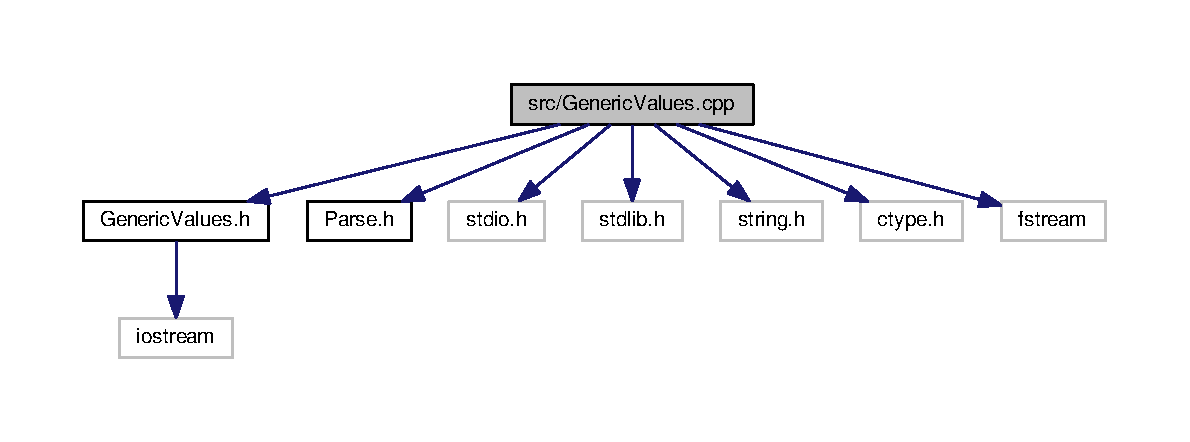
\includegraphics[width=350pt]{GenericValues_8cpp__incl}
\end{center}
\end{figure}


\subsection{Detailed Description}

\begin{DoxyPre}
{\bfseries File:}          \hyperlink{GenericValues_8cpp}{GenericValues.cpp}
{\bfseries Project:}       Robocup Soccer Simulation Team: UvA Trilearn
{\bfseries Authors:}       Jelle Kok
{\bfseries Created:}       28/11/2000
{\bfseries Last Revision:} $ID\$
{\bfseries Contents:}      Code file for classes \hyperlink{classGenericValueT}{GenericValueT} and \hyperlink{classGenericValues}{GenericValues}.
               The class \hyperlink{classGenericValueT}{GenericValueT} contains a pointer to a variable
               of a generic type (double, char*, bool, int). This pointer
               is associated with a string. The class \hyperlink{classGenericValues}{GenericValues}
               contains a collection of \hyperlink{classGenericValueT}{GenericValueT} objects. The member
               method implementations for both classes can be found in
               this file.\end{DoxyPre}
 

 
\begin{DoxyPre}
\subsubsection*{{\bfseries Changes}}\end{DoxyPre}



\begin{DoxyPre}
{\bfseries Date}             {\bfseries Author}          {\bfseries Comment}
28/11/2000       Jelle Kok       Initial version created (based on Emiel Corten)
30/12/2000       Jelle Kok       Initial documentation written
21/05/2001       Remco de Boer   Version including full documentation completed
\end{DoxyPre}
 
\hypertarget{GenericValues_8h}{}\section{src/\+Generic\+Values.h File Reference}
\label{GenericValues_8h}\index{src/\+Generic\+Values.\+h@{src/\+Generic\+Values.\+h}}
{\ttfamily \#include $<$iostream$>$}\\*
Include dependency graph for Generic\+Values.\+h\+:
\nopagebreak
\begin{figure}[H]
\begin{center}
\leavevmode
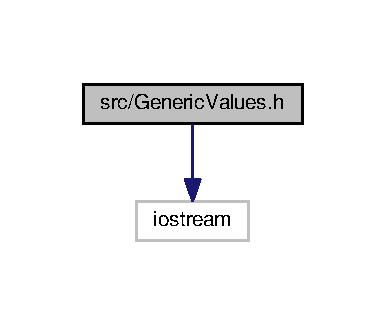
\includegraphics[width=185pt]{GenericValues_8h__incl}
\end{center}
\end{figure}
This graph shows which files directly or indirectly include this file\+:
\nopagebreak
\begin{figure}[H]
\begin{center}
\leavevmode
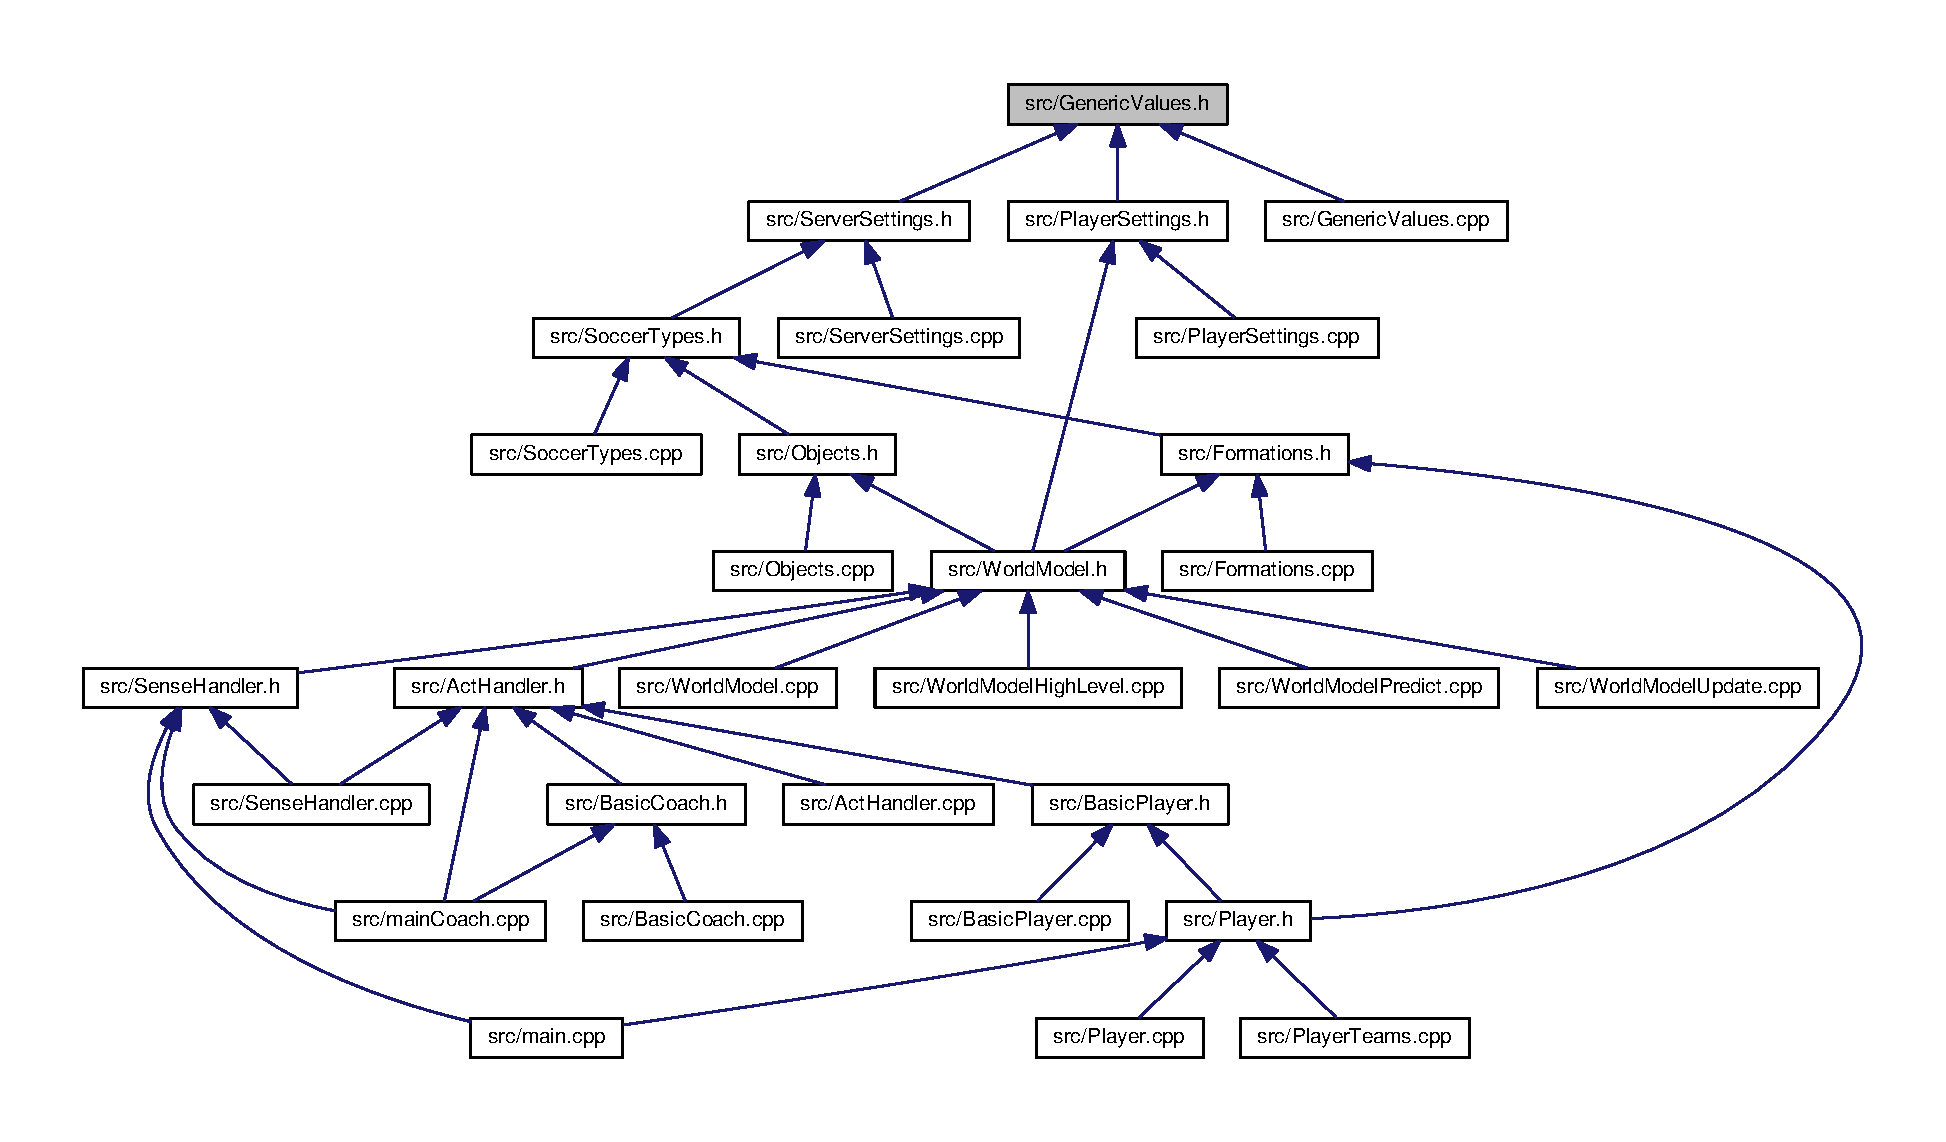
\includegraphics[width=350pt]{GenericValues_8h__dep__incl}
\end{center}
\end{figure}
\subsection*{Classes}
\begin{DoxyCompactItemize}
\item 
class \hyperlink{classGenericValueT}{Generic\+ValueT}
\item 
class \hyperlink{classGenericValues}{Generic\+Values}
\end{DoxyCompactItemize}
\subsection*{Enumerations}
\begin{DoxyCompactItemize}
\item 
enum \hyperlink{GenericValues_8h_aaecaa3e46488aab71938a199e362d0c6}{Generic\+Value\+Kind} \{ {\bfseries G\+E\+N\+E\+R\+I\+C\+\_\+\+V\+A\+L\+U\+E\+\_\+\+D\+O\+U\+B\+LE} = 0, 
{\bfseries G\+E\+N\+E\+R\+I\+C\+\_\+\+V\+A\+L\+U\+E\+\_\+\+S\+T\+R\+I\+NG} = 1, 
{\bfseries G\+E\+N\+E\+R\+I\+C\+\_\+\+V\+A\+L\+U\+E\+\_\+\+B\+O\+O\+L\+E\+AN} = 2, 
{\bfseries G\+E\+N\+E\+R\+I\+C\+\_\+\+V\+A\+L\+U\+E\+\_\+\+I\+N\+T\+E\+G\+ER} = 3
 \}
\end{DoxyCompactItemize}


\subsection{Detailed Description}

\begin{DoxyPre}
{\bfseries File:}          \hyperlink{GenericValues_8h}{GenericValues.h}
{\bfseries Project:}       Robocup Soccer Simulation Team: UvA Trilearn
{\bfseries Authors:}       Jelle Kok
{\bfseries Created:}       28/11/2000
{\bfseries Last Revision:} $ID\$
{\bfseries Contents:}      Header file for classes \hyperlink{classGenericValueT}{GenericValueT} and \hyperlink{classGenericValues}{GenericValues}.
               The class \hyperlink{classGenericValueT}{GenericValueT} contains a pointer to a variable
               of a generic type (double, char*, bool, int). This pointer
               is associated with a string. The class \hyperlink{classGenericValues}{GenericValues}
               contains a collection of \hyperlink{classGenericValueT}{GenericValueT} objects. All the
               member data and member method declarations for both
               classes can be found in this file.\end{DoxyPre}
 

 
\begin{DoxyPre}
\subsubsection*{{\bfseries Changes}}\end{DoxyPre}



\begin{DoxyPre}
{\bfseries Date}             {\bfseries Author}          {\bfseries Comment}
28/11/2000       Jelle Kok       Initial version (based on Emiel Corten)
30/12/2000       Jelle Kok       Initial documentation written
09/05/2001       Remco de Boer   Version including full documentation completed
\end{DoxyPre}
 

\subsection{Enumeration Type Documentation}
\index{Generic\+Values.\+h@{Generic\+Values.\+h}!Generic\+Value\+Kind@{Generic\+Value\+Kind}}
\index{Generic\+Value\+Kind@{Generic\+Value\+Kind}!Generic\+Values.\+h@{Generic\+Values.\+h}}
\subsubsection[{\texorpdfstring{Generic\+Value\+Kind}{GenericValueKind}}]{\setlength{\rightskip}{0pt plus 5cm}enum {\bf Generic\+Value\+Kind}}\hypertarget{GenericValues_8h_aaecaa3e46488aab71938a199e362d0c6}{}\label{GenericValues_8h_aaecaa3e46488aab71938a199e362d0c6}
This enumeration contains all generic values used throughout the code. 
\hypertarget{Geometry_8cpp}{}\section{src/\+Geometry.cpp File Reference}
\label{Geometry_8cpp}\index{src/\+Geometry.\+cpp@{src/\+Geometry.\+cpp}}
{\ttfamily \#include \char`\"{}Geometry.\+h\char`\"{}}\\*
{\ttfamily \#include $<$stdio.\+h$>$}\\*
Include dependency graph for Geometry.\+cpp\+:
\nopagebreak
\begin{figure}[H]
\begin{center}
\leavevmode
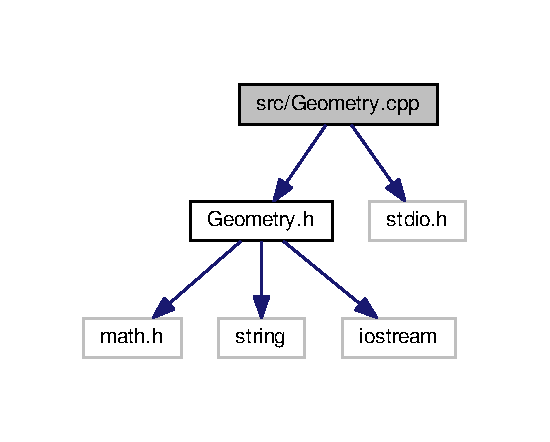
\includegraphics[width=264pt]{Geometry_8cpp__incl}
\end{center}
\end{figure}
\subsection*{Functions}
\begin{DoxyCompactItemize}
\item 
int \hyperlink{Geometry_8cpp_a349dea271f68410c7de1cfcfb5cd518f}{sign} (double d1)
\item 
double \hyperlink{Geometry_8cpp_a0d608373c6f2b9809537cf787583391c}{max} (double d1, double d2)
\item 
double \hyperlink{Geometry_8cpp_acc0c5b1efeaef64a06c0877206917034}{min} (double d1, double d2)
\item 
\hyperlink{Geometry_8h_a6bfe02ae9bb185092902092561ab2865}{Ang\+Deg} \hyperlink{Geometry_8cpp_a331523aca37d4361f3a069fc2459dd1d}{Rad2\+Deg} (\hyperlink{Geometry_8h_a4a8fd1c029bf947992b3d745a2e23363}{Ang\+Rad} x)
\item 
\hyperlink{Geometry_8h_a4a8fd1c029bf947992b3d745a2e23363}{Ang\+Rad} \hyperlink{Geometry_8cpp_ada23931c22ebf0c6f7cd951db289af86}{Deg2\+Rad} (\hyperlink{Geometry_8h_a6bfe02ae9bb185092902092561ab2865}{Ang\+Deg} x)
\item 
double \hyperlink{Geometry_8cpp_afff1ddfe0d946c0e475af137f0b52d12}{cos\+Deg} (\hyperlink{Geometry_8h_a6bfe02ae9bb185092902092561ab2865}{Ang\+Deg} x)
\item 
double \hyperlink{Geometry_8cpp_a9e3698f673d5f5288e373974c5330a2d}{sin\+Deg} (\hyperlink{Geometry_8h_a6bfe02ae9bb185092902092561ab2865}{Ang\+Deg} x)
\item 
double \hyperlink{Geometry_8cpp_ab5e3e3e4597c9fbaac94b80d3d81671b}{tan\+Deg} (\hyperlink{Geometry_8h_a6bfe02ae9bb185092902092561ab2865}{Ang\+Deg} x)
\item 
\hyperlink{Geometry_8h_a6bfe02ae9bb185092902092561ab2865}{Ang\+Deg} \hyperlink{Geometry_8cpp_ac8d0a1881e2bb94ad8fca9a82d0aa356}{atan\+Deg} (double x)
\item 
double \hyperlink{Geometry_8cpp_a3b5a779dcd2d9ed717ba63c19b0ff8fc}{atan2\+Deg} (double x, double y)
\item 
\hyperlink{Geometry_8h_a6bfe02ae9bb185092902092561ab2865}{Ang\+Deg} \hyperlink{Geometry_8cpp_a06baf28df68cfc97dbd667639ade2a5d}{acos\+Deg} (double x)
\item 
\hyperlink{Geometry_8h_a6bfe02ae9bb185092902092561ab2865}{Ang\+Deg} \hyperlink{Geometry_8cpp_a8e8291ab3916da54b792bee7a421cda1}{asin\+Deg} (double x)
\item 
bool \hyperlink{Geometry_8cpp_a1ce8967c983deb94170ddd393ce4db6e}{is\+Ang\+In\+Interval} (\hyperlink{Geometry_8h_a6bfe02ae9bb185092902092561ab2865}{Ang\+Deg} ang, \hyperlink{Geometry_8h_a6bfe02ae9bb185092902092561ab2865}{Ang\+Deg} ang\+Min, \hyperlink{Geometry_8h_a6bfe02ae9bb185092902092561ab2865}{Ang\+Deg} ang\+Max)
\item 
\hyperlink{Geometry_8h_a6bfe02ae9bb185092902092561ab2865}{Ang\+Deg} \hyperlink{Geometry_8cpp_afed76fb3fe11b5d209a32cf5df41be34}{get\+Bisector\+Two\+Angles} (\hyperlink{Geometry_8h_a6bfe02ae9bb185092902092561ab2865}{Ang\+Deg} ang\+Min, \hyperlink{Geometry_8h_a6bfe02ae9bb185092902092561ab2865}{Ang\+Deg} ang\+Max)
\item 
ostream \& \hyperlink{Geometry_8cpp_a93db64ab8b20247fd7e0ec825c8682d0}{operator$<$$<$} (ostream \&os, \hyperlink{classVecPosition}{Vec\+Position} v)
\item 
ostream \& \hyperlink{Geometry_8cpp_af288570ccd047cae99dc45e4743d99ae}{operator$<$$<$} (ostream \&os, \hyperlink{classLine}{Line} l)
\end{DoxyCompactItemize}


\subsection{Detailed Description}

\begin{DoxyPre}
{\bfseries File:}          \hyperlink{Geometry_8cpp}{Geometry.cpp}
{\bfseries Project:}       Robocup Soccer Simulation Team: UvA Trilearn
{\bfseries Authors:}       Jelle Kok
{\bfseries Created:}       13/02/2001
{\bfseries Last Revision:} $ID\$
{\bfseries Contents:}      class declarations of different geometry classes:~\newline

\begin{DoxyItemize}
\item \hyperlink{classVecPosition}{VecPosition}: representation of a point
\item \hyperlink{classLine}{Line}:        representation of a line
\item Rectangle:   representation of a rectangle
\item \hyperlink{classCircle}{Circle}:      representation of a circle
\item \hyperlink{classGeometry}{Geometry}:    different geometry methods
\end{DoxyItemize}\end{DoxyPre}



\begin{DoxyPre}Furthermore it contains some goniometric functions to work with sine, cosine
and tangent functions using degrees and some utility functions to return
the maximum and the minimum of two values.



\subsubsection*{{\bfseries Changes}}\end{DoxyPre}



\begin{DoxyPre}
{\bfseries Date}             {\bfseries Author}          {\bfseries Comment}
12/02/2001       Jelle Kok       Initial version created
\end{DoxyPre}
 

\subsection{Function Documentation}
\index{Geometry.\+cpp@{Geometry.\+cpp}!acos\+Deg@{acos\+Deg}}
\index{acos\+Deg@{acos\+Deg}!Geometry.\+cpp@{Geometry.\+cpp}}
\subsubsection[{\texorpdfstring{acos\+Deg(double x)}{acosDeg(double x)}}]{\setlength{\rightskip}{0pt plus 5cm}{\bf Ang\+Deg} acos\+Deg (
\begin{DoxyParamCaption}
\item[{double}]{x}
\end{DoxyParamCaption}
)}\hypertarget{Geometry_8cpp_a06baf28df68cfc97dbd667639ade2a5d}{}\label{Geometry_8cpp_a06baf28df68cfc97dbd667639ade2a5d}
This function returns the principal value of the arc cosine of x in degrees using the built-\/in arc cosine function which returns this value in radians. 
\begin{DoxyParams}{Parameters}
{\em x} & a double value \\
\hline
\end{DoxyParams}
\begin{DoxyReturn}{Returns}
the arc cosine of the given value in degrees 
\end{DoxyReturn}
\index{Geometry.\+cpp@{Geometry.\+cpp}!asin\+Deg@{asin\+Deg}}
\index{asin\+Deg@{asin\+Deg}!Geometry.\+cpp@{Geometry.\+cpp}}
\subsubsection[{\texorpdfstring{asin\+Deg(double x)}{asinDeg(double x)}}]{\setlength{\rightskip}{0pt plus 5cm}{\bf Ang\+Deg} asin\+Deg (
\begin{DoxyParamCaption}
\item[{double}]{x}
\end{DoxyParamCaption}
)}\hypertarget{Geometry_8cpp_a8e8291ab3916da54b792bee7a421cda1}{}\label{Geometry_8cpp_a8e8291ab3916da54b792bee7a421cda1}
This function returns the principal value of the arc sine of x in degrees using the built-\/in arc sine function which returns this value in radians. 
\begin{DoxyParams}{Parameters}
{\em x} & a double value \\
\hline
\end{DoxyParams}
\begin{DoxyReturn}{Returns}
the arc sine of the given value in degrees 
\end{DoxyReturn}
\index{Geometry.\+cpp@{Geometry.\+cpp}!atan2\+Deg@{atan2\+Deg}}
\index{atan2\+Deg@{atan2\+Deg}!Geometry.\+cpp@{Geometry.\+cpp}}
\subsubsection[{\texorpdfstring{atan2\+Deg(double x, double y)}{atan2Deg(double x, double y)}}]{\setlength{\rightskip}{0pt plus 5cm}double atan2\+Deg (
\begin{DoxyParamCaption}
\item[{double}]{x, }
\item[{double}]{y}
\end{DoxyParamCaption}
)}\hypertarget{Geometry_8cpp_a3b5a779dcd2d9ed717ba63c19b0ff8fc}{}\label{Geometry_8cpp_a3b5a779dcd2d9ed717ba63c19b0ff8fc}
This function returns the principal value of the arc tangent of y/x in degrees using the signs of both arguments to determine the quadrant of the return value. For this the built-\/in \textquotesingle{}atan2\textquotesingle{} function is used which returns this value in radians. 
\begin{DoxyParams}{Parameters}
{\em x} & a double value \\
\hline
{\em y} & a double value \\
\hline
\end{DoxyParams}
\begin{DoxyReturn}{Returns}
the arc tangent of y/x in degrees taking the signs of x and y into account 
\end{DoxyReturn}
\index{Geometry.\+cpp@{Geometry.\+cpp}!atan\+Deg@{atan\+Deg}}
\index{atan\+Deg@{atan\+Deg}!Geometry.\+cpp@{Geometry.\+cpp}}
\subsubsection[{\texorpdfstring{atan\+Deg(double x)}{atanDeg(double x)}}]{\setlength{\rightskip}{0pt plus 5cm}{\bf Ang\+Deg} atan\+Deg (
\begin{DoxyParamCaption}
\item[{double}]{x}
\end{DoxyParamCaption}
)}\hypertarget{Geometry_8cpp_ac8d0a1881e2bb94ad8fca9a82d0aa356}{}\label{Geometry_8cpp_ac8d0a1881e2bb94ad8fca9a82d0aa356}
This function returns the principal value of the arc tangent of x in degrees using the built-\/in arc tangent function which returns this value in radians. 
\begin{DoxyParams}{Parameters}
{\em x} & a double value \\
\hline
\end{DoxyParams}
\begin{DoxyReturn}{Returns}
the arc tangent of the given value in degrees 
\end{DoxyReturn}
\index{Geometry.\+cpp@{Geometry.\+cpp}!cos\+Deg@{cos\+Deg}}
\index{cos\+Deg@{cos\+Deg}!Geometry.\+cpp@{Geometry.\+cpp}}
\subsubsection[{\texorpdfstring{cos\+Deg(\+Ang\+Deg x)}{cosDeg(AngDeg x)}}]{\setlength{\rightskip}{0pt plus 5cm}double cos\+Deg (
\begin{DoxyParamCaption}
\item[{{\bf Ang\+Deg}}]{x}
\end{DoxyParamCaption}
)}\hypertarget{Geometry_8cpp_afff1ddfe0d946c0e475af137f0b52d12}{}\label{Geometry_8cpp_afff1ddfe0d946c0e475af137f0b52d12}
This function returns the cosine of a given angle in degrees using the built-\/in cosine function that works with angles in radians. 
\begin{DoxyParams}{Parameters}
{\em x} & an angle in degrees \\
\hline
\end{DoxyParams}
\begin{DoxyReturn}{Returns}
the cosine of the given angle 
\end{DoxyReturn}
\index{Geometry.\+cpp@{Geometry.\+cpp}!Deg2\+Rad@{Deg2\+Rad}}
\index{Deg2\+Rad@{Deg2\+Rad}!Geometry.\+cpp@{Geometry.\+cpp}}
\subsubsection[{\texorpdfstring{Deg2\+Rad(\+Ang\+Deg x)}{Deg2Rad(AngDeg x)}}]{\setlength{\rightskip}{0pt plus 5cm}{\bf Ang\+Rad} Deg2\+Rad (
\begin{DoxyParamCaption}
\item[{{\bf Ang\+Deg}}]{x}
\end{DoxyParamCaption}
)}\hypertarget{Geometry_8cpp_ada23931c22ebf0c6f7cd951db289af86}{}\label{Geometry_8cpp_ada23931c22ebf0c6f7cd951db289af86}
This function converts an angle in degrees to the corresponding angle in radians. 
\begin{DoxyParams}{Parameters}
{\em x} & an angle in degrees \\
\hline
\end{DoxyParams}
\begin{DoxyReturn}{Returns}
the corresponding angle in radians 
\end{DoxyReturn}
\index{Geometry.\+cpp@{Geometry.\+cpp}!get\+Bisector\+Two\+Angles@{get\+Bisector\+Two\+Angles}}
\index{get\+Bisector\+Two\+Angles@{get\+Bisector\+Two\+Angles}!Geometry.\+cpp@{Geometry.\+cpp}}
\subsubsection[{\texorpdfstring{get\+Bisector\+Two\+Angles(\+Ang\+Deg ang\+Min, Ang\+Deg ang\+Max)}{getBisectorTwoAngles(AngDeg angMin, AngDeg angMax)}}]{\setlength{\rightskip}{0pt plus 5cm}{\bf Ang\+Deg} get\+Bisector\+Two\+Angles (
\begin{DoxyParamCaption}
\item[{{\bf Ang\+Deg}}]{ang\+Min, }
\item[{{\bf Ang\+Deg}}]{ang\+Max}
\end{DoxyParamCaption}
)}\hypertarget{Geometry_8cpp_afed76fb3fe11b5d209a32cf5df41be34}{}\label{Geometry_8cpp_afed76fb3fe11b5d209a32cf5df41be34}
This method returns the bisector (average) of two angles. It deals with the boundary problem, thus when \textquotesingle{}ang\+Min\textquotesingle{} equals 170 and \textquotesingle{}ang\+Max\textquotesingle{} equals -\/100, -\/145 is returned. 
\begin{DoxyParams}{Parameters}
{\em ang\+Min} & minimum angle \mbox{[}-\/180,180\mbox{]} \\
\hline
{\em ang\+Max} & maximum angle \mbox{[}-\/180,180\mbox{]} \\
\hline
\end{DoxyParams}
\begin{DoxyReturn}{Returns}
average of ang\+Min and ang\+Max. 
\end{DoxyReturn}
\index{Geometry.\+cpp@{Geometry.\+cpp}!is\+Ang\+In\+Interval@{is\+Ang\+In\+Interval}}
\index{is\+Ang\+In\+Interval@{is\+Ang\+In\+Interval}!Geometry.\+cpp@{Geometry.\+cpp}}
\subsubsection[{\texorpdfstring{is\+Ang\+In\+Interval(\+Ang\+Deg ang, Ang\+Deg ang\+Min, Ang\+Deg ang\+Max)}{isAngInInterval(AngDeg ang, AngDeg angMin, AngDeg angMax)}}]{\setlength{\rightskip}{0pt plus 5cm}bool is\+Ang\+In\+Interval (
\begin{DoxyParamCaption}
\item[{{\bf Ang\+Deg}}]{ang, }
\item[{{\bf Ang\+Deg}}]{ang\+Min, }
\item[{{\bf Ang\+Deg}}]{ang\+Max}
\end{DoxyParamCaption}
)}\hypertarget{Geometry_8cpp_a1ce8967c983deb94170ddd393ce4db6e}{}\label{Geometry_8cpp_a1ce8967c983deb94170ddd393ce4db6e}
This function returns a boolean value which indicates whether the value \textquotesingle{}ang\textquotesingle{} (from interval \mbox{[}-\/180..180\mbox{]} lies in the interval \mbox{[}ang\+Min..ang\+Max\mbox{]}. Examples\+: is\+Ang\+In\+Interval( -\/100, 4, -\/150) returns false is\+Ang\+In\+Interval( 45, 4, -\/150) returns true 
\begin{DoxyParams}{Parameters}
{\em ang} & angle that should be checked \\
\hline
{\em ang\+Min} & minimum angle in interval \\
\hline
{\em ang\+Max} & maximum angle in interval \\
\hline
\end{DoxyParams}
\begin{DoxyReturn}{Returns}
boolean indicating whether ang lies in \mbox{[}ang\+Min..ang\+Max\mbox{]} 
\end{DoxyReturn}
\index{Geometry.\+cpp@{Geometry.\+cpp}!max@{max}}
\index{max@{max}!Geometry.\+cpp@{Geometry.\+cpp}}
\subsubsection[{\texorpdfstring{max(double d1, double d2)}{max(double d1, double d2)}}]{\setlength{\rightskip}{0pt plus 5cm}double max (
\begin{DoxyParamCaption}
\item[{double}]{d1, }
\item[{double}]{d2}
\end{DoxyParamCaption}
)}\hypertarget{Geometry_8cpp_a0d608373c6f2b9809537cf787583391c}{}\label{Geometry_8cpp_a0d608373c6f2b9809537cf787583391c}
This function returns the maximum of two given doubles. 
\begin{DoxyParams}{Parameters}
{\em d1} & first parameter \\
\hline
{\em d2} & second parameter \\
\hline
\end{DoxyParams}
\begin{DoxyReturn}{Returns}
the maximum of these two parameters 
\end{DoxyReturn}
\index{Geometry.\+cpp@{Geometry.\+cpp}!min@{min}}
\index{min@{min}!Geometry.\+cpp@{Geometry.\+cpp}}
\subsubsection[{\texorpdfstring{min(double d1, double d2)}{min(double d1, double d2)}}]{\setlength{\rightskip}{0pt plus 5cm}double min (
\begin{DoxyParamCaption}
\item[{double}]{d1, }
\item[{double}]{d2}
\end{DoxyParamCaption}
)}\hypertarget{Geometry_8cpp_acc0c5b1efeaef64a06c0877206917034}{}\label{Geometry_8cpp_acc0c5b1efeaef64a06c0877206917034}
This function returns the minimum of two given doubles. 
\begin{DoxyParams}{Parameters}
{\em d1} & first parameter \\
\hline
{\em d2} & second parameter \\
\hline
\end{DoxyParams}
\begin{DoxyReturn}{Returns}
the minimum of these two parameters 
\end{DoxyReturn}
\index{Geometry.\+cpp@{Geometry.\+cpp}!operator$<$$<$@{operator$<$$<$}}
\index{operator$<$$<$@{operator$<$$<$}!Geometry.\+cpp@{Geometry.\+cpp}}
\subsubsection[{\texorpdfstring{operator$<$$<$(ostream \&os, Vec\+Position v)}{operator<<(ostream &os, VecPosition v)}}]{\setlength{\rightskip}{0pt plus 5cm}ostream\& operator$<$$<$ (
\begin{DoxyParamCaption}
\item[{ostream \&}]{os, }
\item[{{\bf Vec\+Position}}]{v}
\end{DoxyParamCaption}
)}\hypertarget{Geometry_8cpp_a93db64ab8b20247fd7e0ec825c8682d0}{}\label{Geometry_8cpp_a93db64ab8b20247fd7e0ec825c8682d0}
Overloaded version of the C++ output operator for Vec\+Positions. This operator makes it possible to use Vec\+Positions in output statements (e.\+g. cout $<$$<$ v). The x-\/ and y-\/coordinates of the \hyperlink{classVecPosition}{Vec\+Position} are printed in the format (x,y).


\begin{DoxyParams}{Parameters}
{\em os} & output stream to which information should be written \\
\hline
{\em v} & a \hyperlink{classVecPosition}{Vec\+Position} which must be printed \\
\hline
\end{DoxyParams}
\begin{DoxyReturn}{Returns}
output stream containing (x,y) 
\end{DoxyReturn}
\index{Geometry.\+cpp@{Geometry.\+cpp}!operator$<$$<$@{operator$<$$<$}}
\index{operator$<$$<$@{operator$<$$<$}!Geometry.\+cpp@{Geometry.\+cpp}}
\subsubsection[{\texorpdfstring{operator$<$$<$(ostream \&os, Line l)}{operator<<(ostream &os, Line l)}}]{\setlength{\rightskip}{0pt plus 5cm}ostream\& operator$<$$<$ (
\begin{DoxyParamCaption}
\item[{ostream \&}]{os, }
\item[{{\bf Line}}]{l}
\end{DoxyParamCaption}
)}\hypertarget{Geometry_8cpp_af288570ccd047cae99dc45e4743d99ae}{}\label{Geometry_8cpp_af288570ccd047cae99dc45e4743d99ae}
This function prints the line to the specified output stream in the format y = ax + b. 
\begin{DoxyParams}{Parameters}
{\em os} & output stream to which output is written \\
\hline
{\em l} & line that is written to output stream \\
\hline
\end{DoxyParams}
\begin{DoxyReturn}{Returns}
output sream to which output is appended. 
\end{DoxyReturn}
\index{Geometry.\+cpp@{Geometry.\+cpp}!Rad2\+Deg@{Rad2\+Deg}}
\index{Rad2\+Deg@{Rad2\+Deg}!Geometry.\+cpp@{Geometry.\+cpp}}
\subsubsection[{\texorpdfstring{Rad2\+Deg(\+Ang\+Rad x)}{Rad2Deg(AngRad x)}}]{\setlength{\rightskip}{0pt plus 5cm}{\bf Ang\+Deg} Rad2\+Deg (
\begin{DoxyParamCaption}
\item[{{\bf Ang\+Rad}}]{x}
\end{DoxyParamCaption}
)}\hypertarget{Geometry_8cpp_a331523aca37d4361f3a069fc2459dd1d}{}\label{Geometry_8cpp_a331523aca37d4361f3a069fc2459dd1d}
This function converts an angle in radians to the corresponding angle in degrees. 
\begin{DoxyParams}{Parameters}
{\em x} & an angle in radians \\
\hline
\end{DoxyParams}
\begin{DoxyReturn}{Returns}
the corresponding angle in degrees 
\end{DoxyReturn}
\index{Geometry.\+cpp@{Geometry.\+cpp}!sign@{sign}}
\index{sign@{sign}!Geometry.\+cpp@{Geometry.\+cpp}}
\subsubsection[{\texorpdfstring{sign(double d1)}{sign(double d1)}}]{\setlength{\rightskip}{0pt plus 5cm}int sign (
\begin{DoxyParamCaption}
\item[{double}]{d1}
\end{DoxyParamCaption}
)}\hypertarget{Geometry_8cpp_a349dea271f68410c7de1cfcfb5cd518f}{}\label{Geometry_8cpp_a349dea271f68410c7de1cfcfb5cd518f}
This function returns the sign of a give double. 1 is positive, -\/1 is negative 
\begin{DoxyParams}{Parameters}
{\em d1} & first parameter \\
\hline
\end{DoxyParams}
\begin{DoxyReturn}{Returns}
the sign of this double 
\end{DoxyReturn}
\index{Geometry.\+cpp@{Geometry.\+cpp}!sin\+Deg@{sin\+Deg}}
\index{sin\+Deg@{sin\+Deg}!Geometry.\+cpp@{Geometry.\+cpp}}
\subsubsection[{\texorpdfstring{sin\+Deg(\+Ang\+Deg x)}{sinDeg(AngDeg x)}}]{\setlength{\rightskip}{0pt plus 5cm}double sin\+Deg (
\begin{DoxyParamCaption}
\item[{{\bf Ang\+Deg}}]{x}
\end{DoxyParamCaption}
)}\hypertarget{Geometry_8cpp_a9e3698f673d5f5288e373974c5330a2d}{}\label{Geometry_8cpp_a9e3698f673d5f5288e373974c5330a2d}
This function returns the sine of a given angle in degrees using the built-\/in sine function that works with angles in radians. 
\begin{DoxyParams}{Parameters}
{\em x} & an angle in degrees \\
\hline
\end{DoxyParams}
\begin{DoxyReturn}{Returns}
the sine of the given angle 
\end{DoxyReturn}
\index{Geometry.\+cpp@{Geometry.\+cpp}!tan\+Deg@{tan\+Deg}}
\index{tan\+Deg@{tan\+Deg}!Geometry.\+cpp@{Geometry.\+cpp}}
\subsubsection[{\texorpdfstring{tan\+Deg(\+Ang\+Deg x)}{tanDeg(AngDeg x)}}]{\setlength{\rightskip}{0pt plus 5cm}double tan\+Deg (
\begin{DoxyParamCaption}
\item[{{\bf Ang\+Deg}}]{x}
\end{DoxyParamCaption}
)}\hypertarget{Geometry_8cpp_ab5e3e3e4597c9fbaac94b80d3d81671b}{}\label{Geometry_8cpp_ab5e3e3e4597c9fbaac94b80d3d81671b}
This function returns the tangent of a given angle in degrees using the built-\/in tangent function that works with angles in radians. 
\begin{DoxyParams}{Parameters}
{\em x} & an angle in degrees \\
\hline
\end{DoxyParams}
\begin{DoxyReturn}{Returns}
the tangent of the given angle 
\end{DoxyReturn}

\hypertarget{Geometry_8h}{}\section{src/\+Geometry.h File Reference}
\label{Geometry_8h}\index{src/\+Geometry.\+h@{src/\+Geometry.\+h}}
{\ttfamily \#include \char`\"{}math.\+h\char`\"{}}\\*
{\ttfamily \#include $<$string$>$}\\*
{\ttfamily \#include $<$iostream$>$}\\*
Include dependency graph for Geometry.\+h\+:
\nopagebreak
\begin{figure}[H]
\begin{center}
\leavevmode
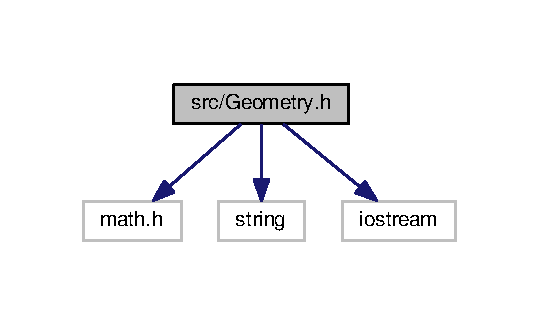
\includegraphics[width=259pt]{Geometry_8h__incl}
\end{center}
\end{figure}
This graph shows which files directly or indirectly include this file\+:
\nopagebreak
\begin{figure}[H]
\begin{center}
\leavevmode
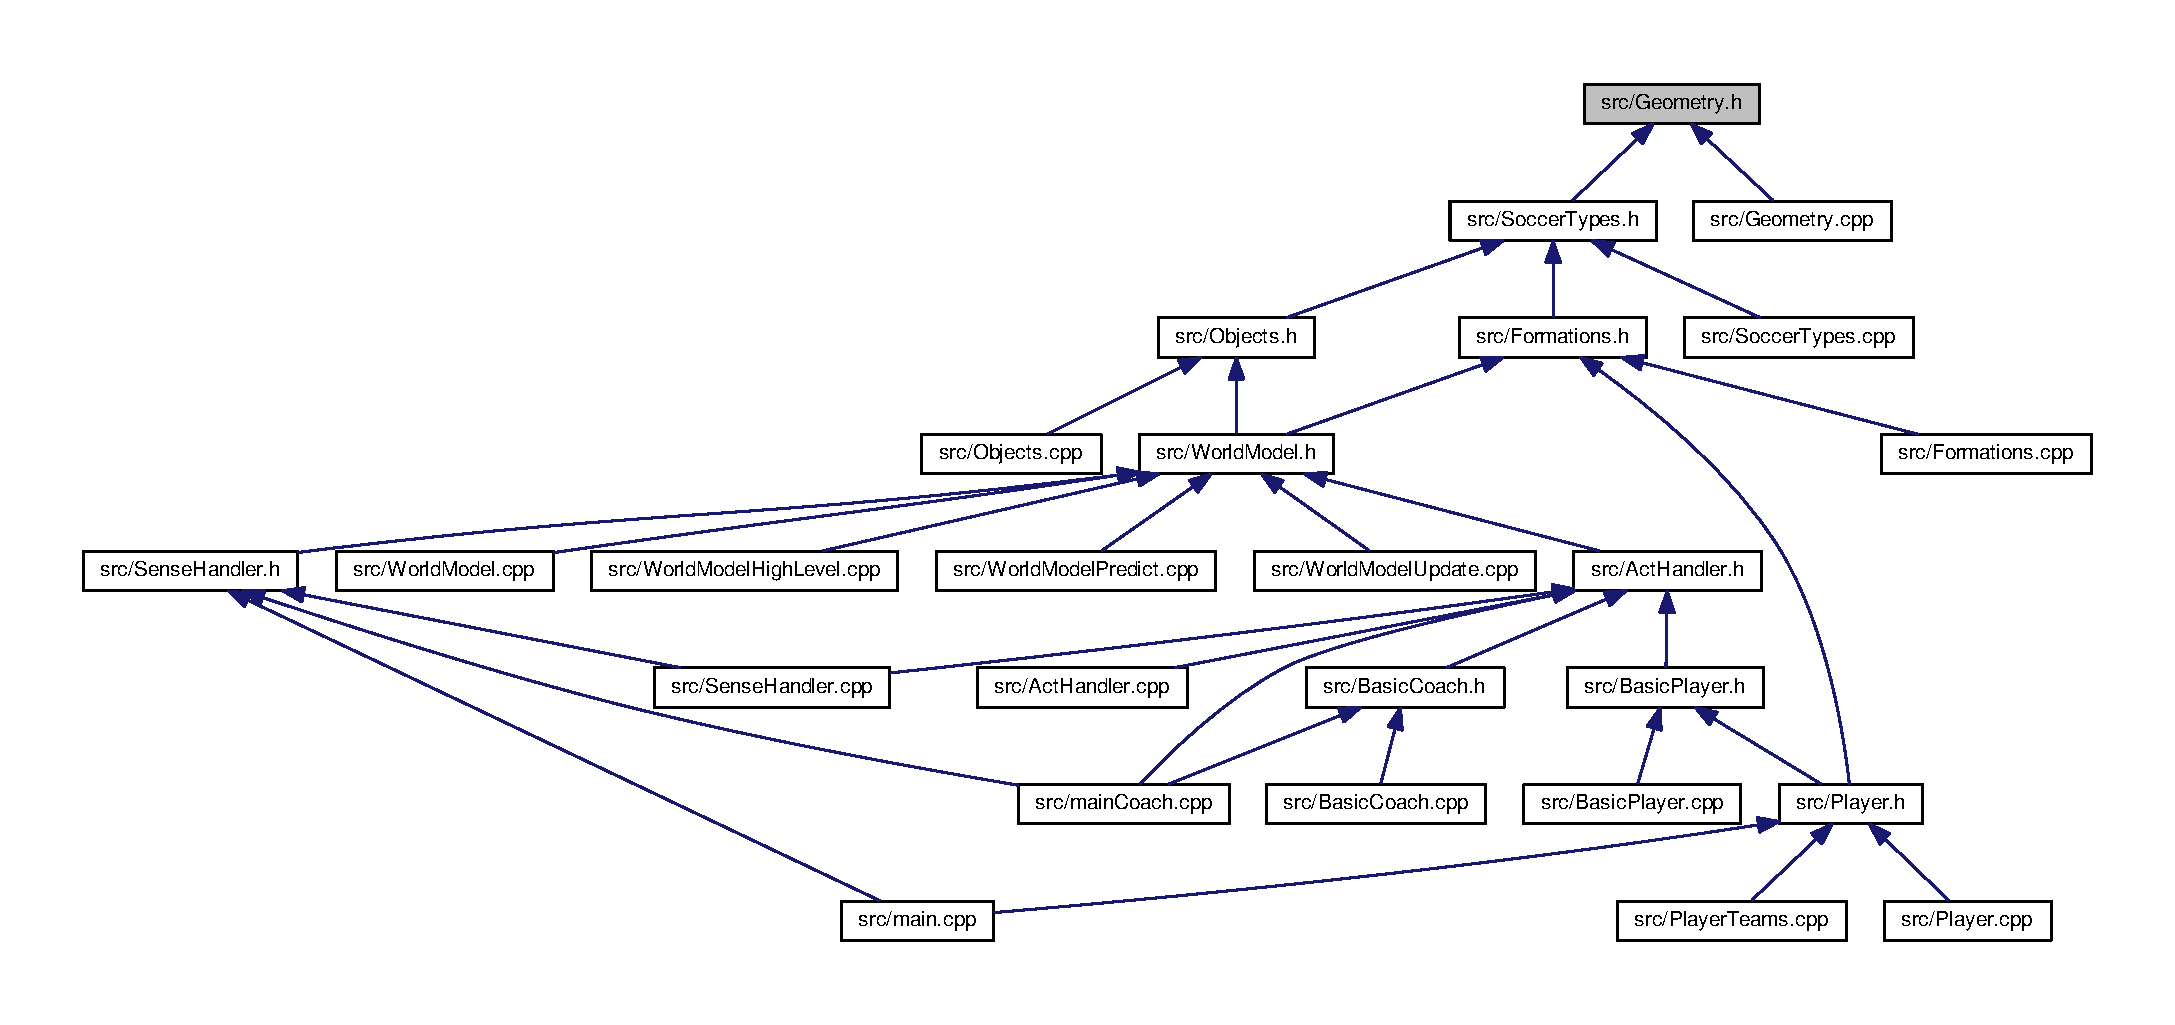
\includegraphics[width=350pt]{Geometry_8h__dep__incl}
\end{center}
\end{figure}
\subsection*{Classes}
\begin{DoxyCompactItemize}
\item 
class \hyperlink{classVecPosition}{Vec\+Position}
\item 
class \hyperlink{classGeometry}{Geometry}
\item 
class \hyperlink{classCircle}{Circle}
\item 
class \hyperlink{classLine}{Line}
\item 
class \hyperlink{classRect}{Rect}
\end{DoxyCompactItemize}
\subsection*{Macros}
\begin{DoxyCompactItemize}
\item 
\#define \hyperlink{Geometry_8h_a002b2f4894492820fe708b1b7e7c5e70}{E\+P\+S\+I\+L\+ON}~0.\+0001
\end{DoxyCompactItemize}
\subsection*{Typedefs}
\begin{DoxyCompactItemize}
\item 
typedef double \hyperlink{Geometry_8h_a4a8fd1c029bf947992b3d745a2e23363}{Ang\+Rad}
\item 
typedef double \hyperlink{Geometry_8h_a6bfe02ae9bb185092902092561ab2865}{Ang\+Deg}
\end{DoxyCompactItemize}
\subsection*{Enumerations}
\begin{DoxyCompactItemize}
\item 
enum \hyperlink{Geometry_8h_af3e194d00b468bcd9641c4d3576a0624}{Coord\+SystemT} \{ {\bfseries C\+A\+R\+T\+E\+S\+I\+AN}, 
{\bfseries P\+O\+L\+AR}
 \}
\end{DoxyCompactItemize}
\subsection*{Functions}
\begin{DoxyCompactItemize}
\item 
double \hyperlink{Geometry_8h_a0d608373c6f2b9809537cf787583391c}{max} (double d1, double d2)
\item 
double \hyperlink{Geometry_8h_acc0c5b1efeaef64a06c0877206917034}{min} (double d1, double d2)
\item 
int \hyperlink{Geometry_8h_a349dea271f68410c7de1cfcfb5cd518f}{sign} (double d1)
\item 
\hyperlink{Geometry_8h_a6bfe02ae9bb185092902092561ab2865}{Ang\+Deg} \hyperlink{Geometry_8h_a331523aca37d4361f3a069fc2459dd1d}{Rad2\+Deg} (\hyperlink{Geometry_8h_a4a8fd1c029bf947992b3d745a2e23363}{Ang\+Rad} x)
\item 
\hyperlink{Geometry_8h_a4a8fd1c029bf947992b3d745a2e23363}{Ang\+Rad} \hyperlink{Geometry_8h_ada23931c22ebf0c6f7cd951db289af86}{Deg2\+Rad} (\hyperlink{Geometry_8h_a6bfe02ae9bb185092902092561ab2865}{Ang\+Deg} x)
\item 
double \hyperlink{Geometry_8h_afff1ddfe0d946c0e475af137f0b52d12}{cos\+Deg} (\hyperlink{Geometry_8h_a6bfe02ae9bb185092902092561ab2865}{Ang\+Deg} x)
\item 
double \hyperlink{Geometry_8h_a9e3698f673d5f5288e373974c5330a2d}{sin\+Deg} (\hyperlink{Geometry_8h_a6bfe02ae9bb185092902092561ab2865}{Ang\+Deg} x)
\item 
double \hyperlink{Geometry_8h_ab5e3e3e4597c9fbaac94b80d3d81671b}{tan\+Deg} (\hyperlink{Geometry_8h_a6bfe02ae9bb185092902092561ab2865}{Ang\+Deg} x)
\item 
\hyperlink{Geometry_8h_a6bfe02ae9bb185092902092561ab2865}{Ang\+Deg} \hyperlink{Geometry_8h_ac8d0a1881e2bb94ad8fca9a82d0aa356}{atan\+Deg} (double x)
\item 
double \hyperlink{Geometry_8h_a3b5a779dcd2d9ed717ba63c19b0ff8fc}{atan2\+Deg} (double x, double y)
\item 
\hyperlink{Geometry_8h_a6bfe02ae9bb185092902092561ab2865}{Ang\+Deg} \hyperlink{Geometry_8h_a06baf28df68cfc97dbd667639ade2a5d}{acos\+Deg} (double x)
\item 
\hyperlink{Geometry_8h_a6bfe02ae9bb185092902092561ab2865}{Ang\+Deg} \hyperlink{Geometry_8h_a8e8291ab3916da54b792bee7a421cda1}{asin\+Deg} (double x)
\item 
bool \hyperlink{Geometry_8h_a1ce8967c983deb94170ddd393ce4db6e}{is\+Ang\+In\+Interval} (\hyperlink{Geometry_8h_a6bfe02ae9bb185092902092561ab2865}{Ang\+Deg} ang, \hyperlink{Geometry_8h_a6bfe02ae9bb185092902092561ab2865}{Ang\+Deg} ang\+Min, \hyperlink{Geometry_8h_a6bfe02ae9bb185092902092561ab2865}{Ang\+Deg} ang\+Max)
\item 
\hyperlink{Geometry_8h_a6bfe02ae9bb185092902092561ab2865}{Ang\+Deg} \hyperlink{Geometry_8h_afed76fb3fe11b5d209a32cf5df41be34}{get\+Bisector\+Two\+Angles} (\hyperlink{Geometry_8h_a6bfe02ae9bb185092902092561ab2865}{Ang\+Deg} ang\+Min, \hyperlink{Geometry_8h_a6bfe02ae9bb185092902092561ab2865}{Ang\+Deg} ang\+Max)
\end{DoxyCompactItemize}


\subsection{Detailed Description}

\begin{DoxyPre}
{\bfseries File:}          \hyperlink{Geometry_8h}{Geometry.h}
{\bfseries Project:}       Robocup Soccer Simulation Team: UvA Trilearn
{\bfseries Authors:}       Jelle Kok
{\bfseries Created:}       12/02/2001
{\bfseries Last Revision:} $ID\$
{\bfseries Contents:}      Header file for the classes \hyperlink{classVecPosition}{VecPosition}, \hyperlink{classGeometry}{Geometry}, \hyperlink{classLine}{Line},
               \hyperlink{classCircle}{Circle} and Rectangle. All the member
               data and member method declarations for all these classes can be
               found in this file together with some auxiliary functions for
               numeric and goniometric purposes.



\subsubsection*{{\bfseries Changes}}\end{DoxyPre}



\begin{DoxyPre}
{\bfseries Date}             {\bfseries Author}          {\bfseries Comment}
12/02/2001       Jelle Kok       Initial version created
09/06/2001       Remco de Boer   Version including full documentation completed
\end{DoxyPre}
 

\subsection{Macro Definition Documentation}
\index{Geometry.\+h@{Geometry.\+h}!E\+P\+S\+I\+L\+ON@{E\+P\+S\+I\+L\+ON}}
\index{E\+P\+S\+I\+L\+ON@{E\+P\+S\+I\+L\+ON}!Geometry.\+h@{Geometry.\+h}}
\subsubsection[{\texorpdfstring{E\+P\+S\+I\+L\+ON}{EPSILON}}]{\setlength{\rightskip}{0pt plus 5cm}\#define E\+P\+S\+I\+L\+ON~0.\+0001}\hypertarget{Geometry_8h_a002b2f4894492820fe708b1b7e7c5e70}{}\label{Geometry_8h_a002b2f4894492820fe708b1b7e7c5e70}
Value used for floating point equality tests. 

\subsection{Typedef Documentation}
\index{Geometry.\+h@{Geometry.\+h}!Ang\+Deg@{Ang\+Deg}}
\index{Ang\+Deg@{Ang\+Deg}!Geometry.\+h@{Geometry.\+h}}
\subsubsection[{\texorpdfstring{Ang\+Deg}{AngDeg}}]{\setlength{\rightskip}{0pt plus 5cm}typedef double {\bf Ang\+Deg}}\hypertarget{Geometry_8h_a6bfe02ae9bb185092902092561ab2865}{}\label{Geometry_8h_a6bfe02ae9bb185092902092561ab2865}
Type definition for angles in radians. \index{Geometry.\+h@{Geometry.\+h}!Ang\+Rad@{Ang\+Rad}}
\index{Ang\+Rad@{Ang\+Rad}!Geometry.\+h@{Geometry.\+h}}
\subsubsection[{\texorpdfstring{Ang\+Rad}{AngRad}}]{\setlength{\rightskip}{0pt plus 5cm}typedef double {\bf Ang\+Rad}}\hypertarget{Geometry_8h_a4a8fd1c029bf947992b3d745a2e23363}{}\label{Geometry_8h_a4a8fd1c029bf947992b3d745a2e23363}
Type definition for angles in degrees. 

\subsection{Enumeration Type Documentation}
\index{Geometry.\+h@{Geometry.\+h}!Coord\+SystemT@{Coord\+SystemT}}
\index{Coord\+SystemT@{Coord\+SystemT}!Geometry.\+h@{Geometry.\+h}}
\subsubsection[{\texorpdfstring{Coord\+SystemT}{CoordSystemT}}]{\setlength{\rightskip}{0pt plus 5cm}enum {\bf Coord\+SystemT}}\hypertarget{Geometry_8h_af3e194d00b468bcd9641c4d3576a0624}{}\label{Geometry_8h_af3e194d00b468bcd9641c4d3576a0624}
Coord\+System is an enumeration of the different specified coordinate systems. The two possibilities are C\+A\+R\+T\+E\+S\+I\+AN or P\+O\+L\+AR. These values are for instance used in the initializing a \hyperlink{classVecPosition}{Vec\+Position}. The Coord\+System indicates whether the supplied arguments represent the position in cartesian or in polar coordinates. 

\subsection{Function Documentation}
\index{Geometry.\+h@{Geometry.\+h}!acos\+Deg@{acos\+Deg}}
\index{acos\+Deg@{acos\+Deg}!Geometry.\+h@{Geometry.\+h}}
\subsubsection[{\texorpdfstring{acos\+Deg(double x)}{acosDeg(double x)}}]{\setlength{\rightskip}{0pt plus 5cm}{\bf Ang\+Deg} acos\+Deg (
\begin{DoxyParamCaption}
\item[{double}]{x}
\end{DoxyParamCaption}
)}\hypertarget{Geometry_8h_a06baf28df68cfc97dbd667639ade2a5d}{}\label{Geometry_8h_a06baf28df68cfc97dbd667639ade2a5d}
This function returns the principal value of the arc cosine of x in degrees using the built-\/in arc cosine function which returns this value in radians. 
\begin{DoxyParams}{Parameters}
{\em x} & a double value \\
\hline
\end{DoxyParams}
\begin{DoxyReturn}{Returns}
the arc cosine of the given value in degrees 
\end{DoxyReturn}
\index{Geometry.\+h@{Geometry.\+h}!asin\+Deg@{asin\+Deg}}
\index{asin\+Deg@{asin\+Deg}!Geometry.\+h@{Geometry.\+h}}
\subsubsection[{\texorpdfstring{asin\+Deg(double x)}{asinDeg(double x)}}]{\setlength{\rightskip}{0pt plus 5cm}{\bf Ang\+Deg} asin\+Deg (
\begin{DoxyParamCaption}
\item[{double}]{x}
\end{DoxyParamCaption}
)}\hypertarget{Geometry_8h_a8e8291ab3916da54b792bee7a421cda1}{}\label{Geometry_8h_a8e8291ab3916da54b792bee7a421cda1}
This function returns the principal value of the arc sine of x in degrees using the built-\/in arc sine function which returns this value in radians. 
\begin{DoxyParams}{Parameters}
{\em x} & a double value \\
\hline
\end{DoxyParams}
\begin{DoxyReturn}{Returns}
the arc sine of the given value in degrees 
\end{DoxyReturn}
\index{Geometry.\+h@{Geometry.\+h}!atan2\+Deg@{atan2\+Deg}}
\index{atan2\+Deg@{atan2\+Deg}!Geometry.\+h@{Geometry.\+h}}
\subsubsection[{\texorpdfstring{atan2\+Deg(double x, double y)}{atan2Deg(double x, double y)}}]{\setlength{\rightskip}{0pt plus 5cm}double atan2\+Deg (
\begin{DoxyParamCaption}
\item[{double}]{x, }
\item[{double}]{y}
\end{DoxyParamCaption}
)}\hypertarget{Geometry_8h_a3b5a779dcd2d9ed717ba63c19b0ff8fc}{}\label{Geometry_8h_a3b5a779dcd2d9ed717ba63c19b0ff8fc}
This function returns the principal value of the arc tangent of y/x in degrees using the signs of both arguments to determine the quadrant of the return value. For this the built-\/in \textquotesingle{}atan2\textquotesingle{} function is used which returns this value in radians. 
\begin{DoxyParams}{Parameters}
{\em x} & a double value \\
\hline
{\em y} & a double value \\
\hline
\end{DoxyParams}
\begin{DoxyReturn}{Returns}
the arc tangent of y/x in degrees taking the signs of x and y into account 
\end{DoxyReturn}
\index{Geometry.\+h@{Geometry.\+h}!atan\+Deg@{atan\+Deg}}
\index{atan\+Deg@{atan\+Deg}!Geometry.\+h@{Geometry.\+h}}
\subsubsection[{\texorpdfstring{atan\+Deg(double x)}{atanDeg(double x)}}]{\setlength{\rightskip}{0pt plus 5cm}{\bf Ang\+Deg} atan\+Deg (
\begin{DoxyParamCaption}
\item[{double}]{x}
\end{DoxyParamCaption}
)}\hypertarget{Geometry_8h_ac8d0a1881e2bb94ad8fca9a82d0aa356}{}\label{Geometry_8h_ac8d0a1881e2bb94ad8fca9a82d0aa356}
This function returns the principal value of the arc tangent of x in degrees using the built-\/in arc tangent function which returns this value in radians. 
\begin{DoxyParams}{Parameters}
{\em x} & a double value \\
\hline
\end{DoxyParams}
\begin{DoxyReturn}{Returns}
the arc tangent of the given value in degrees 
\end{DoxyReturn}
\index{Geometry.\+h@{Geometry.\+h}!cos\+Deg@{cos\+Deg}}
\index{cos\+Deg@{cos\+Deg}!Geometry.\+h@{Geometry.\+h}}
\subsubsection[{\texorpdfstring{cos\+Deg(\+Ang\+Deg x)}{cosDeg(AngDeg x)}}]{\setlength{\rightskip}{0pt plus 5cm}double cos\+Deg (
\begin{DoxyParamCaption}
\item[{{\bf Ang\+Deg}}]{x}
\end{DoxyParamCaption}
)}\hypertarget{Geometry_8h_afff1ddfe0d946c0e475af137f0b52d12}{}\label{Geometry_8h_afff1ddfe0d946c0e475af137f0b52d12}
This function returns the cosine of a given angle in degrees using the built-\/in cosine function that works with angles in radians. 
\begin{DoxyParams}{Parameters}
{\em x} & an angle in degrees \\
\hline
\end{DoxyParams}
\begin{DoxyReturn}{Returns}
the cosine of the given angle 
\end{DoxyReturn}
\index{Geometry.\+h@{Geometry.\+h}!Deg2\+Rad@{Deg2\+Rad}}
\index{Deg2\+Rad@{Deg2\+Rad}!Geometry.\+h@{Geometry.\+h}}
\subsubsection[{\texorpdfstring{Deg2\+Rad(\+Ang\+Deg x)}{Deg2Rad(AngDeg x)}}]{\setlength{\rightskip}{0pt plus 5cm}{\bf Ang\+Rad} Deg2\+Rad (
\begin{DoxyParamCaption}
\item[{{\bf Ang\+Deg}}]{x}
\end{DoxyParamCaption}
)}\hypertarget{Geometry_8h_ada23931c22ebf0c6f7cd951db289af86}{}\label{Geometry_8h_ada23931c22ebf0c6f7cd951db289af86}
This function converts an angle in degrees to the corresponding angle in radians. 
\begin{DoxyParams}{Parameters}
{\em x} & an angle in degrees \\
\hline
\end{DoxyParams}
\begin{DoxyReturn}{Returns}
the corresponding angle in radians 
\end{DoxyReturn}
\index{Geometry.\+h@{Geometry.\+h}!get\+Bisector\+Two\+Angles@{get\+Bisector\+Two\+Angles}}
\index{get\+Bisector\+Two\+Angles@{get\+Bisector\+Two\+Angles}!Geometry.\+h@{Geometry.\+h}}
\subsubsection[{\texorpdfstring{get\+Bisector\+Two\+Angles(\+Ang\+Deg ang\+Min, Ang\+Deg ang\+Max)}{getBisectorTwoAngles(AngDeg angMin, AngDeg angMax)}}]{\setlength{\rightskip}{0pt plus 5cm}{\bf Ang\+Deg} get\+Bisector\+Two\+Angles (
\begin{DoxyParamCaption}
\item[{{\bf Ang\+Deg}}]{ang\+Min, }
\item[{{\bf Ang\+Deg}}]{ang\+Max}
\end{DoxyParamCaption}
)}\hypertarget{Geometry_8h_afed76fb3fe11b5d209a32cf5df41be34}{}\label{Geometry_8h_afed76fb3fe11b5d209a32cf5df41be34}
This method returns the bisector (average) of two angles. It deals with the boundary problem, thus when \textquotesingle{}ang\+Min\textquotesingle{} equals 170 and \textquotesingle{}ang\+Max\textquotesingle{} equals -\/100, -\/145 is returned. 
\begin{DoxyParams}{Parameters}
{\em ang\+Min} & minimum angle \mbox{[}-\/180,180\mbox{]} \\
\hline
{\em ang\+Max} & maximum angle \mbox{[}-\/180,180\mbox{]} \\
\hline
\end{DoxyParams}
\begin{DoxyReturn}{Returns}
average of ang\+Min and ang\+Max. 
\end{DoxyReturn}
\index{Geometry.\+h@{Geometry.\+h}!is\+Ang\+In\+Interval@{is\+Ang\+In\+Interval}}
\index{is\+Ang\+In\+Interval@{is\+Ang\+In\+Interval}!Geometry.\+h@{Geometry.\+h}}
\subsubsection[{\texorpdfstring{is\+Ang\+In\+Interval(\+Ang\+Deg ang, Ang\+Deg ang\+Min, Ang\+Deg ang\+Max)}{isAngInInterval(AngDeg ang, AngDeg angMin, AngDeg angMax)}}]{\setlength{\rightskip}{0pt plus 5cm}bool is\+Ang\+In\+Interval (
\begin{DoxyParamCaption}
\item[{{\bf Ang\+Deg}}]{ang, }
\item[{{\bf Ang\+Deg}}]{ang\+Min, }
\item[{{\bf Ang\+Deg}}]{ang\+Max}
\end{DoxyParamCaption}
)}\hypertarget{Geometry_8h_a1ce8967c983deb94170ddd393ce4db6e}{}\label{Geometry_8h_a1ce8967c983deb94170ddd393ce4db6e}
This function returns a boolean value which indicates whether the value \textquotesingle{}ang\textquotesingle{} (from interval \mbox{[}-\/180..180\mbox{]} lies in the interval \mbox{[}ang\+Min..ang\+Max\mbox{]}. Examples\+: is\+Ang\+In\+Interval( -\/100, 4, -\/150) returns false is\+Ang\+In\+Interval( 45, 4, -\/150) returns true 
\begin{DoxyParams}{Parameters}
{\em ang} & angle that should be checked \\
\hline
{\em ang\+Min} & minimum angle in interval \\
\hline
{\em ang\+Max} & maximum angle in interval \\
\hline
\end{DoxyParams}
\begin{DoxyReturn}{Returns}
boolean indicating whether ang lies in \mbox{[}ang\+Min..ang\+Max\mbox{]} 
\end{DoxyReturn}
\index{Geometry.\+h@{Geometry.\+h}!max@{max}}
\index{max@{max}!Geometry.\+h@{Geometry.\+h}}
\subsubsection[{\texorpdfstring{max(double d1, double d2)}{max(double d1, double d2)}}]{\setlength{\rightskip}{0pt plus 5cm}double max (
\begin{DoxyParamCaption}
\item[{double}]{d1, }
\item[{double}]{d2}
\end{DoxyParamCaption}
)}\hypertarget{Geometry_8h_a0d608373c6f2b9809537cf787583391c}{}\label{Geometry_8h_a0d608373c6f2b9809537cf787583391c}
This function returns the maximum of two given doubles. 
\begin{DoxyParams}{Parameters}
{\em d1} & first parameter \\
\hline
{\em d2} & second parameter \\
\hline
\end{DoxyParams}
\begin{DoxyReturn}{Returns}
the maximum of these two parameters 
\end{DoxyReturn}
\index{Geometry.\+h@{Geometry.\+h}!min@{min}}
\index{min@{min}!Geometry.\+h@{Geometry.\+h}}
\subsubsection[{\texorpdfstring{min(double d1, double d2)}{min(double d1, double d2)}}]{\setlength{\rightskip}{0pt plus 5cm}double min (
\begin{DoxyParamCaption}
\item[{double}]{d1, }
\item[{double}]{d2}
\end{DoxyParamCaption}
)}\hypertarget{Geometry_8h_acc0c5b1efeaef64a06c0877206917034}{}\label{Geometry_8h_acc0c5b1efeaef64a06c0877206917034}
This function returns the minimum of two given doubles. 
\begin{DoxyParams}{Parameters}
{\em d1} & first parameter \\
\hline
{\em d2} & second parameter \\
\hline
\end{DoxyParams}
\begin{DoxyReturn}{Returns}
the minimum of these two parameters 
\end{DoxyReturn}
\index{Geometry.\+h@{Geometry.\+h}!Rad2\+Deg@{Rad2\+Deg}}
\index{Rad2\+Deg@{Rad2\+Deg}!Geometry.\+h@{Geometry.\+h}}
\subsubsection[{\texorpdfstring{Rad2\+Deg(\+Ang\+Rad x)}{Rad2Deg(AngRad x)}}]{\setlength{\rightskip}{0pt plus 5cm}{\bf Ang\+Deg} Rad2\+Deg (
\begin{DoxyParamCaption}
\item[{{\bf Ang\+Rad}}]{x}
\end{DoxyParamCaption}
)}\hypertarget{Geometry_8h_a331523aca37d4361f3a069fc2459dd1d}{}\label{Geometry_8h_a331523aca37d4361f3a069fc2459dd1d}
This function converts an angle in radians to the corresponding angle in degrees. 
\begin{DoxyParams}{Parameters}
{\em x} & an angle in radians \\
\hline
\end{DoxyParams}
\begin{DoxyReturn}{Returns}
the corresponding angle in degrees 
\end{DoxyReturn}
\index{Geometry.\+h@{Geometry.\+h}!sign@{sign}}
\index{sign@{sign}!Geometry.\+h@{Geometry.\+h}}
\subsubsection[{\texorpdfstring{sign(double d1)}{sign(double d1)}}]{\setlength{\rightskip}{0pt plus 5cm}int sign (
\begin{DoxyParamCaption}
\item[{double}]{d1}
\end{DoxyParamCaption}
)}\hypertarget{Geometry_8h_a349dea271f68410c7de1cfcfb5cd518f}{}\label{Geometry_8h_a349dea271f68410c7de1cfcfb5cd518f}
This function returns the sign of a give double. 1 is positive, -\/1 is negative 
\begin{DoxyParams}{Parameters}
{\em d1} & first parameter \\
\hline
\end{DoxyParams}
\begin{DoxyReturn}{Returns}
the sign of this double 
\end{DoxyReturn}
\index{Geometry.\+h@{Geometry.\+h}!sin\+Deg@{sin\+Deg}}
\index{sin\+Deg@{sin\+Deg}!Geometry.\+h@{Geometry.\+h}}
\subsubsection[{\texorpdfstring{sin\+Deg(\+Ang\+Deg x)}{sinDeg(AngDeg x)}}]{\setlength{\rightskip}{0pt plus 5cm}double sin\+Deg (
\begin{DoxyParamCaption}
\item[{{\bf Ang\+Deg}}]{x}
\end{DoxyParamCaption}
)}\hypertarget{Geometry_8h_a9e3698f673d5f5288e373974c5330a2d}{}\label{Geometry_8h_a9e3698f673d5f5288e373974c5330a2d}
This function returns the sine of a given angle in degrees using the built-\/in sine function that works with angles in radians. 
\begin{DoxyParams}{Parameters}
{\em x} & an angle in degrees \\
\hline
\end{DoxyParams}
\begin{DoxyReturn}{Returns}
the sine of the given angle 
\end{DoxyReturn}
\index{Geometry.\+h@{Geometry.\+h}!tan\+Deg@{tan\+Deg}}
\index{tan\+Deg@{tan\+Deg}!Geometry.\+h@{Geometry.\+h}}
\subsubsection[{\texorpdfstring{tan\+Deg(\+Ang\+Deg x)}{tanDeg(AngDeg x)}}]{\setlength{\rightskip}{0pt plus 5cm}double tan\+Deg (
\begin{DoxyParamCaption}
\item[{{\bf Ang\+Deg}}]{x}
\end{DoxyParamCaption}
)}\hypertarget{Geometry_8h_ab5e3e3e4597c9fbaac94b80d3d81671b}{}\label{Geometry_8h_ab5e3e3e4597c9fbaac94b80d3d81671b}
This function returns the tangent of a given angle in degrees using the built-\/in tangent function that works with angles in radians. 
\begin{DoxyParams}{Parameters}
{\em x} & an angle in degrees \\
\hline
\end{DoxyParams}
\begin{DoxyReturn}{Returns}
the tangent of the given angle 
\end{DoxyReturn}

\hypertarget{Logger_8cpp}{}\section{src/\+Logger.cpp File Reference}
\label{Logger_8cpp}\index{src/\+Logger.\+cpp@{src/\+Logger.\+cpp}}
{\ttfamily \#include \char`\"{}Logger.\+h\char`\"{}}\\*
{\ttfamily \#include $<$stdio.\+h$>$}\\*
{\ttfamily \#include $<$string$>$}\\*
{\ttfamily \#include $<$stdarg.\+h$>$}\\*
{\ttfamily \#include $<$pthread.\+h$>$}\\*
{\ttfamily \#include $<$string.\+h$>$}\\*
Include dependency graph for Logger.\+cpp\+:
\nopagebreak
\begin{figure}[H]
\begin{center}
\leavevmode
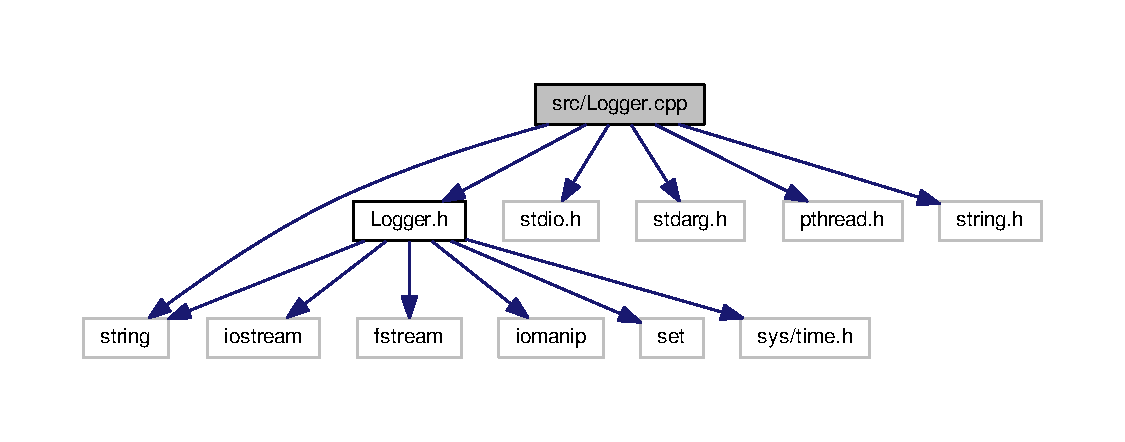
\includegraphics[width=350pt]{Logger_8cpp__incl}
\end{center}
\end{figure}
\subsection*{Variables}
\begin{DoxyCompactItemize}
\item 
\hyperlink{classLogger}{Logger} \hyperlink{Logger_8cpp_af2ed886ec3d2b2fd42fd0c5dad2f8cc5}{Log}
\item 
\hyperlink{classLogger}{Logger} \hyperlink{Logger_8cpp_aa27e9e4165f446c3246f7ba5a5ac677f}{Log\+Draw}
\end{DoxyCompactItemize}


\subsection{Detailed Description}

\begin{DoxyPre}
{\bfseries File:}          \hyperlink{Logger_8cpp}{Logger.cpp}
{\bfseries Project:}       Robocup Soccer Simulation Team: UvA Trilearn
{\bfseries Authors:}       Jelle Kok
{\bfseries Created:}       3/3/2000
{\bfseries Last Revision:} $ID\$
{\bfseries Contents:}      This file contains the definitions for the class to log
               information about the system to any output stream. A
               range can be specified for which the received log
               information is printed. Furthermore it is possible to
               print the time since the timer of the \hyperlink{classLogger}{Logger} has been
               restarted.



\subsubsection*{{\bfseries Changes}}\end{DoxyPre}



\begin{DoxyPre}
{\bfseries Date}             {\bfseries Author}          {\bfseries Comment}
3/3/2001         Jelle Kok       Initial version created
\end{DoxyPre}
 

\subsection{Variable Documentation}
\index{Logger.\+cpp@{Logger.\+cpp}!Log@{Log}}
\index{Log@{Log}!Logger.\+cpp@{Logger.\+cpp}}
\subsubsection[{\texorpdfstring{Log}{Log}}]{\setlength{\rightskip}{0pt plus 5cm}{\bf Logger} Log}\hypertarget{Logger_8cpp_af2ed886ec3d2b2fd42fd0c5dad2f8cc5}{}\label{Logger_8cpp_af2ed886ec3d2b2fd42fd0c5dad2f8cc5}
\hyperlink{classLogger}{Logger} instantation that can be used by all classes \index{Logger.\+cpp@{Logger.\+cpp}!Log\+Draw@{Log\+Draw}}
\index{Log\+Draw@{Log\+Draw}!Logger.\+cpp@{Logger.\+cpp}}
\subsubsection[{\texorpdfstring{Log\+Draw}{LogDraw}}]{\setlength{\rightskip}{0pt plus 5cm}{\bf Logger} Log\+Draw}\hypertarget{Logger_8cpp_aa27e9e4165f446c3246f7ba5a5ac677f}{}\label{Logger_8cpp_aa27e9e4165f446c3246f7ba5a5ac677f}
Drawing logger instantation for all classes 
\hypertarget{Logger_8h}{}\section{src/\+Logger.h File Reference}
\label{Logger_8h}\index{src/\+Logger.\+h@{src/\+Logger.\+h}}
{\ttfamily \#include $<$iostream$>$}\\*
{\ttfamily \#include $<$fstream$>$}\\*
{\ttfamily \#include $<$string$>$}\\*
{\ttfamily \#include $<$iomanip$>$}\\*
{\ttfamily \#include $<$set$>$}\\*
{\ttfamily \#include $<$sys/time.\+h$>$}\\*
Include dependency graph for Logger.\+h\+:
\nopagebreak
\begin{figure}[H]
\begin{center}
\leavevmode
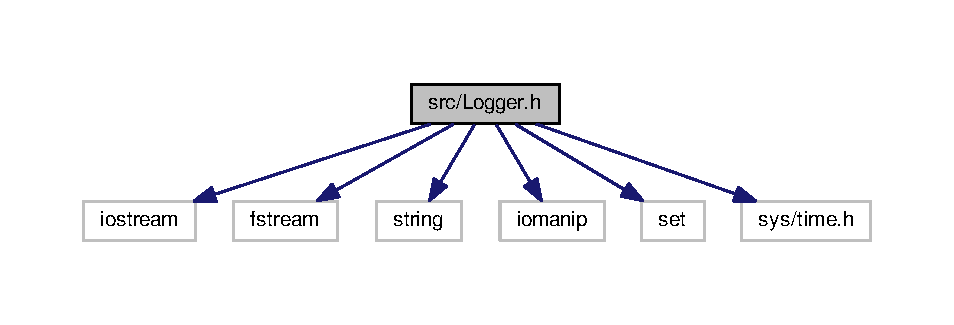
\includegraphics[width=350pt]{Logger_8h__incl}
\end{center}
\end{figure}
This graph shows which files directly or indirectly include this file\+:
\nopagebreak
\begin{figure}[H]
\begin{center}
\leavevmode
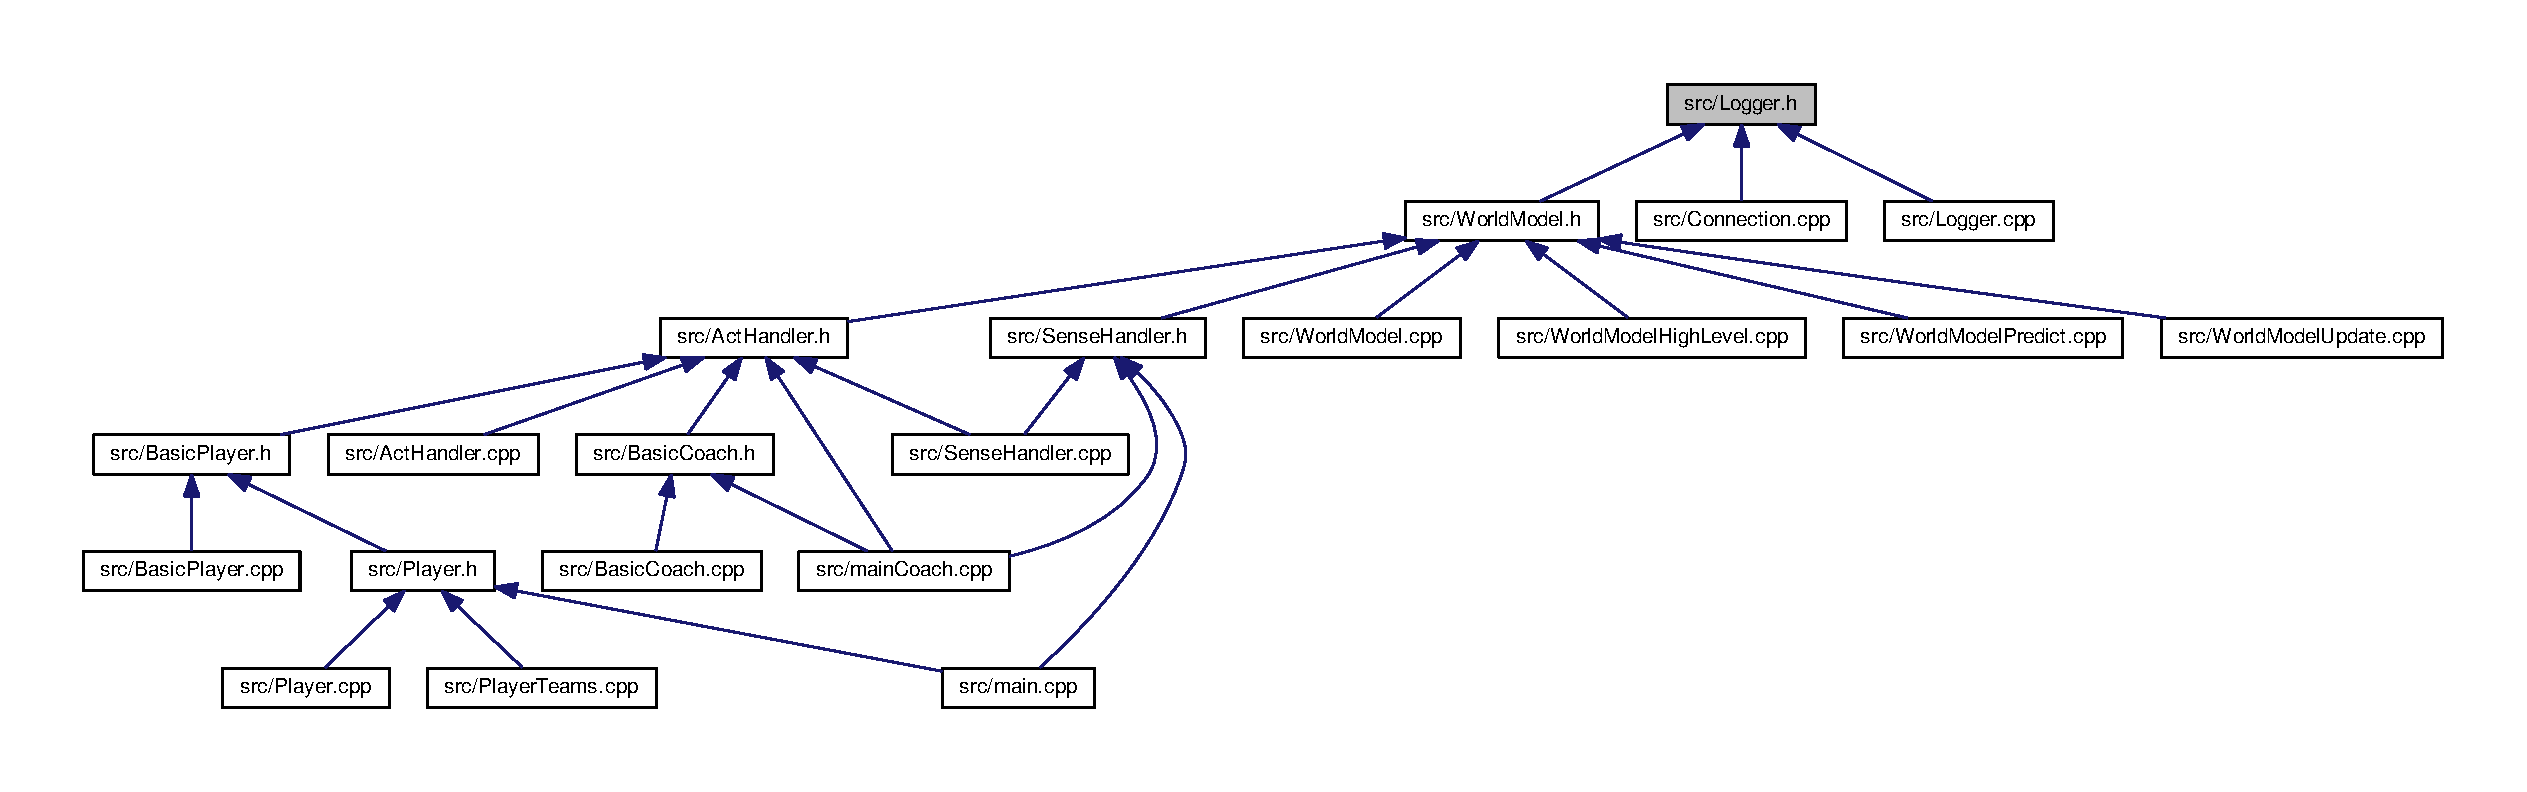
\includegraphics[width=350pt]{Logger_8h__dep__incl}
\end{center}
\end{figure}
\subsection*{Classes}
\begin{DoxyCompactItemize}
\item 
class \hyperlink{classTiming}{Timing}
\item 
class \hyperlink{classLogger}{Logger}
\end{DoxyCompactItemize}
\subsection*{Macros}
\begin{DoxyCompactItemize}
\item 
\#define \hyperlink{Logger_8h_ad1ad1107b2fb6e51cd78d16a64920eca}{M\+A\+X\+\_\+\+L\+O\+G\+\_\+\+L\+I\+NE}~3072
\item 
\#define \hyperlink{Logger_8h_ab400cc7c8787796a32ff06fb899a9ac2}{M\+A\+X\+\_\+\+H\+E\+A\+D\+ER}~128
\end{DoxyCompactItemize}


\subsection{Detailed Description}

\begin{DoxyPre}
{\bfseries File:}          \hyperlink{Logger_8h}{Logger.h}
{\bfseries Project:}       Robocup Soccer Simulation Team: UvA Trilearn
{\bfseries Authors:}       Jelle Kok
{\bfseries Created:}       3/3/2000
{\bfseries Last Revision:} $ID\$
{\bfseries Contents:}      This file contains the class to log information about the
               system to any output stream. A range can be specified
               for which the received log information is printed.
               Furthermore it is possible to print the time since the
               timer of the \hyperlink{classLogger}{Logger} has been restarted.



\subsubsection*{{\bfseries Changes}}\end{DoxyPre}



\begin{DoxyPre}
{\bfseries Date}             {\bfseries Author}          {\bfseries Comment}
3/3/2001         Jelle Kok       Initial version created
\end{DoxyPre}
 

\subsection{Macro Definition Documentation}
\index{Logger.\+h@{Logger.\+h}!M\+A\+X\+\_\+\+H\+E\+A\+D\+ER@{M\+A\+X\+\_\+\+H\+E\+A\+D\+ER}}
\index{M\+A\+X\+\_\+\+H\+E\+A\+D\+ER@{M\+A\+X\+\_\+\+H\+E\+A\+D\+ER}!Logger.\+h@{Logger.\+h}}
\subsubsection[{\texorpdfstring{M\+A\+X\+\_\+\+H\+E\+A\+D\+ER}{MAX_HEADER}}]{\setlength{\rightskip}{0pt plus 5cm}\#define M\+A\+X\+\_\+\+H\+E\+A\+D\+ER~128}\hypertarget{Logger_8h_ab400cc7c8787796a32ff06fb899a9ac2}{}\label{Logger_8h_ab400cc7c8787796a32ff06fb899a9ac2}
maximum size of the header \index{Logger.\+h@{Logger.\+h}!M\+A\+X\+\_\+\+L\+O\+G\+\_\+\+L\+I\+NE@{M\+A\+X\+\_\+\+L\+O\+G\+\_\+\+L\+I\+NE}}
\index{M\+A\+X\+\_\+\+L\+O\+G\+\_\+\+L\+I\+NE@{M\+A\+X\+\_\+\+L\+O\+G\+\_\+\+L\+I\+NE}!Logger.\+h@{Logger.\+h}}
\subsubsection[{\texorpdfstring{M\+A\+X\+\_\+\+L\+O\+G\+\_\+\+L\+I\+NE}{MAX_LOG_LINE}}]{\setlength{\rightskip}{0pt plus 5cm}\#define M\+A\+X\+\_\+\+L\+O\+G\+\_\+\+L\+I\+NE~3072}\hypertarget{Logger_8h_ad1ad1107b2fb6e51cd78d16a64920eca}{}\label{Logger_8h_ad1ad1107b2fb6e51cd78d16a64920eca}
maximum size of a log message 
\hypertarget{main_8cpp}{}\section{src/main.cpp File Reference}
\label{main_8cpp}\index{src/main.\+cpp@{src/main.\+cpp}}
{\ttfamily \#include \char`\"{}Sense\+Handler.\+h\char`\"{}}\\*
{\ttfamily \#include \char`\"{}Player.\+h\char`\"{}}\\*
{\ttfamily \#include \char`\"{}Parse.\+h\char`\"{}}\\*
{\ttfamily \#include $<$string.\+h$>$}\\*
{\ttfamily \#include $<$pthread.\+h$>$}\\*
{\ttfamily \#include $<$stdlib.\+h$>$}\\*
Include dependency graph for main.\+cpp\+:
\nopagebreak
\begin{figure}[H]
\begin{center}
\leavevmode
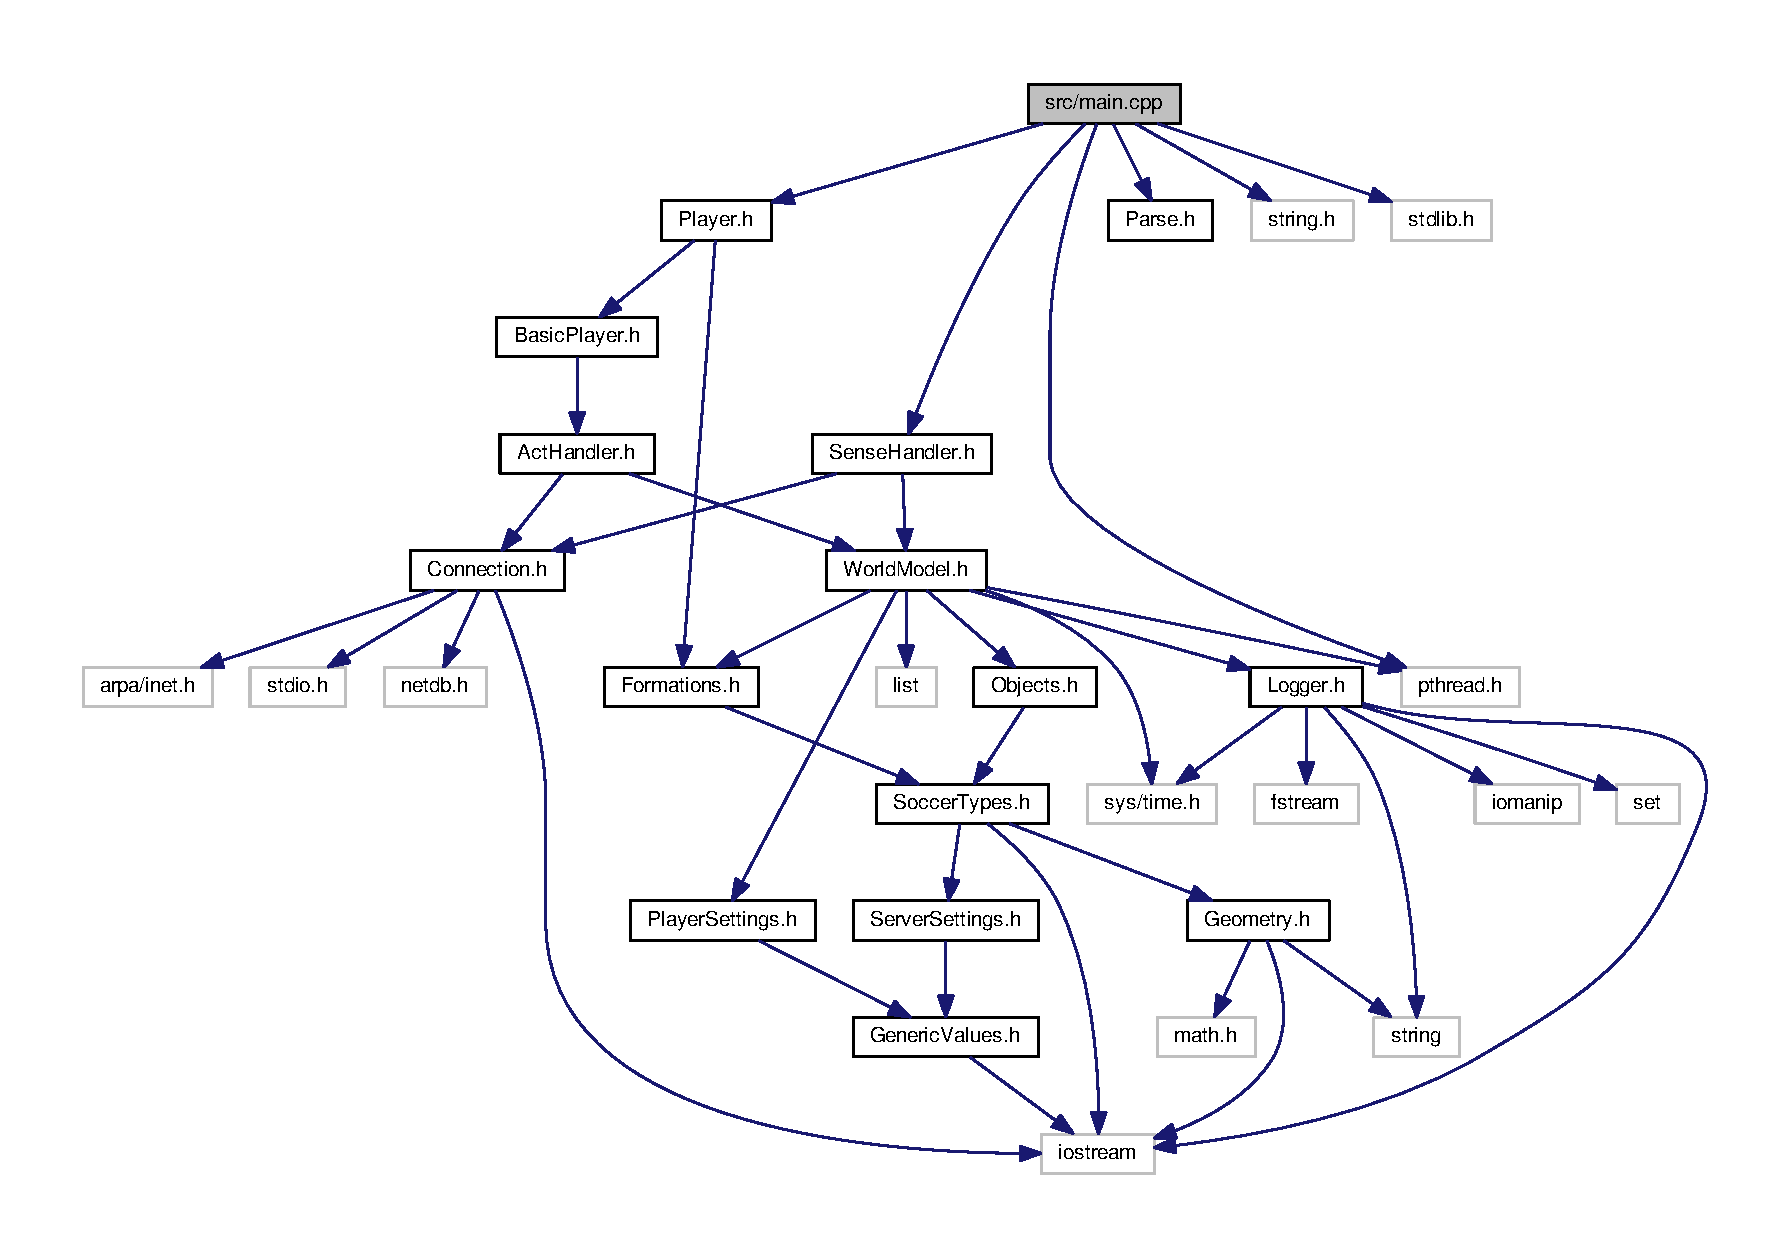
\includegraphics[width=350pt]{main_8cpp__incl}
\end{center}
\end{figure}
\subsection*{Functions}
\begin{DoxyCompactItemize}
\item 
void \hyperlink{main_8cpp_ad67b05b9ebc559482ce6a39423b421c9}{print\+Options} ()
\item 
int \hyperlink{main_8cpp_a0ddf1224851353fc92bfbff6f499fa97}{main} (int argc, char $\ast$argv\mbox{[}$\,$\mbox{]})
\end{DoxyCompactItemize}
\subsection*{Variables}
\begin{DoxyCompactItemize}
\item 
\hyperlink{classLogger}{Logger} \hyperlink{main_8cpp_af2ed886ec3d2b2fd42fd0c5dad2f8cc5}{Log}
\item 
\hyperlink{classLogger}{Logger} \hyperlink{main_8cpp_aa27e9e4165f446c3246f7ba5a5ac677f}{Log\+Draw}
\end{DoxyCompactItemize}


\subsection{Detailed Description}

\begin{DoxyPre}
{\bfseries File:}          \hyperlink{main_8cpp}{main.cpp}
{\bfseries Project:}       Robocup Soccer Simulation Team: UvA Trilearn
{\bfseries Authors:}       Jelle Kok
{\bfseries Created:}       28/11/2000
{\bfseries Last Revision:} $ID\$
{\bfseries Contents:}      This file contains the main of the program that is used
               to start the agent. It creates all classes, starts the different
               threads and calls the mainloop. Furthermore it parses the
               specified arguments to adjust the variables.



\subsubsection*{{\bfseries Changes}}\end{DoxyPre}



\begin{DoxyPre}
{\bfseries Date}             {\bfseries Author}          {\bfseries Comment}
28/11/2000       Jelle Kok       Initial version created
\end{DoxyPre}
 

\subsection{Function Documentation}
\index{main.\+cpp@{main.\+cpp}!main@{main}}
\index{main@{main}!main.\+cpp@{main.\+cpp}}
\subsubsection[{\texorpdfstring{main(int argc, char $\ast$argv[])}{main(int argc, char *argv[])}}]{\setlength{\rightskip}{0pt plus 5cm}int main (
\begin{DoxyParamCaption}
\item[{int}]{argc, }
\item[{char $\ast$}]{argv\mbox{[}$\,$\mbox{]}}
\end{DoxyParamCaption}
)}\hypertarget{main_8cpp_a0ddf1224851353fc92bfbff6f499fa97}{}\label{main_8cpp_a0ddf1224851353fc92bfbff6f499fa97}
This is the main function and creates and links all the different classes. First it reads in all the parameters from the command prompt ($<$program name$>$=\char`\"{}\char`\"{}$>$ -\/help) and uses these values to create the classes. After all the classes are linked, the main\+Loop in the \hyperlink{classPlayer}{Player} class is called. \index{main.\+cpp@{main.\+cpp}!print\+Options@{print\+Options}}
\index{print\+Options@{print\+Options}!main.\+cpp@{main.\+cpp}}
\subsubsection[{\texorpdfstring{print\+Options()}{printOptions()}}]{\setlength{\rightskip}{0pt plus 5cm}void print\+Options (
\begin{DoxyParamCaption}
{}
\end{DoxyParamCaption}
)}\hypertarget{main_8cpp_ad67b05b9ebc559482ce6a39423b421c9}{}\label{main_8cpp_ad67b05b9ebc559482ce6a39423b421c9}
This function prints the command prompt options that can be supplied to the program. 

\subsection{Variable Documentation}
\index{main.\+cpp@{main.\+cpp}!Log@{Log}}
\index{Log@{Log}!main.\+cpp@{main.\+cpp}}
\subsubsection[{\texorpdfstring{Log}{Log}}]{\setlength{\rightskip}{0pt plus 5cm}{\bf Logger} Log}\hypertarget{main_8cpp_af2ed886ec3d2b2fd42fd0c5dad2f8cc5}{}\label{main_8cpp_af2ed886ec3d2b2fd42fd0c5dad2f8cc5}
This is a reference to the normal \hyperlink{classLogger}{Logger} class

\hyperlink{classLogger}{Logger} instantation that can be used by all classes \index{main.\+cpp@{main.\+cpp}!Log\+Draw@{Log\+Draw}}
\index{Log\+Draw@{Log\+Draw}!main.\+cpp@{main.\+cpp}}
\subsubsection[{\texorpdfstring{Log\+Draw}{LogDraw}}]{\setlength{\rightskip}{0pt plus 5cm}{\bf Logger} Log\+Draw}\hypertarget{main_8cpp_aa27e9e4165f446c3246f7ba5a5ac677f}{}\label{main_8cpp_aa27e9e4165f446c3246f7ba5a5ac677f}
This is a reference to the drawing \hyperlink{classLogger}{Logger} class

Drawing logger instantation for all classes 
\hypertarget{mainCoach_8cpp}{}\section{src/main\+Coach.cpp File Reference}
\label{mainCoach_8cpp}\index{src/main\+Coach.\+cpp@{src/main\+Coach.\+cpp}}
{\ttfamily \#include \char`\"{}Act\+Handler.\+h\char`\"{}}\\*
{\ttfamily \#include \char`\"{}Sense\+Handler.\+h\char`\"{}}\\*
{\ttfamily \#include \char`\"{}Basic\+Coach.\+h\char`\"{}}\\*
{\ttfamily \#include \char`\"{}Parse.\+h\char`\"{}}\\*
{\ttfamily \#include $<$string.\+h$>$}\\*
{\ttfamily \#include $<$pthread.\+h$>$}\\*
{\ttfamily \#include $<$stdlib.\+h$>$}\\*
Include dependency graph for main\+Coach.\+cpp\+:
\nopagebreak
\begin{figure}[H]
\begin{center}
\leavevmode
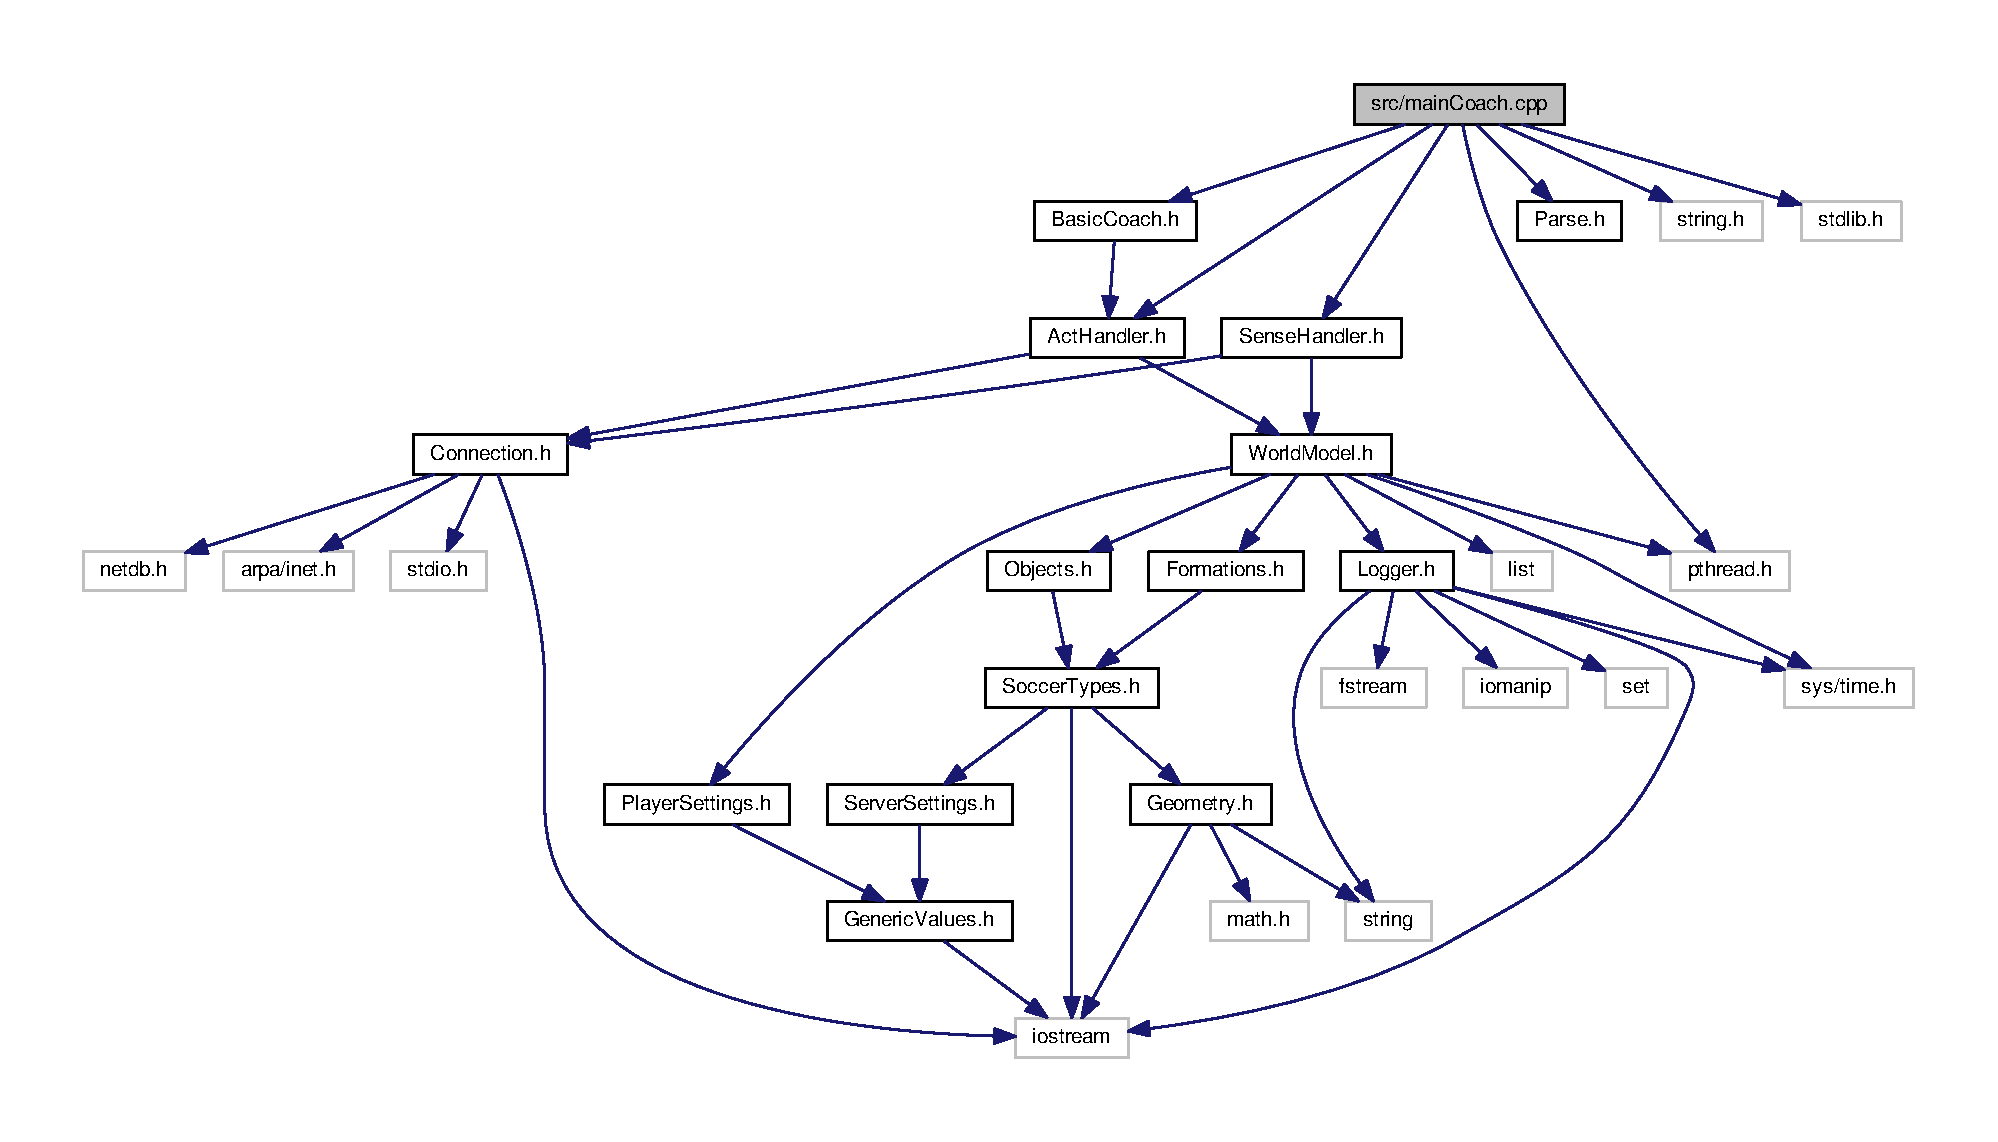
\includegraphics[width=350pt]{mainCoach_8cpp__incl}
\end{center}
\end{figure}
\subsection*{Functions}
\begin{DoxyCompactItemize}
\item 
void \hyperlink{mainCoach_8cpp_ad67b05b9ebc559482ce6a39423b421c9}{print\+Options} ()
\item 
int \hyperlink{mainCoach_8cpp_a0ddf1224851353fc92bfbff6f499fa97}{main} (int argc, char $\ast$argv\mbox{[}$\,$\mbox{]})
\end{DoxyCompactItemize}
\subsection*{Variables}
\begin{DoxyCompactItemize}
\item 
\hyperlink{classLogger}{Logger} \hyperlink{mainCoach_8cpp_af2ed886ec3d2b2fd42fd0c5dad2f8cc5}{Log}
\end{DoxyCompactItemize}


\subsection{Detailed Description}

\begin{DoxyPre}
{\bfseries File:}          \hyperlink{mainCoach_8cpp}{mainCoach.cpp}
{\bfseries Project:}       Robocup Soccer Simulation Team: UvA Trilearn
{\bfseries Authors:}       Jelle Kok
{\bfseries Created:}       28/11/2000
{\bfseries Last Revision:} $ID\$
{\bfseries Contents:}      This file contains the main of the program that is used
                      to start the coach. It creates
                      all classes, starts the different threads and calls the
                      mainloop. Furthermore it parses the incoming arguments
                      to adjust the variables.



\subsubsection*{{\bfseries Changes}}\end{DoxyPre}



\begin{DoxyPre}
{\bfseries Date}             {\bfseries Author}          {\bfseries Comment}
28/11/2000       Jelle Kok       Initial version created
\end{DoxyPre}
 

\subsection{Function Documentation}
\index{main\+Coach.\+cpp@{main\+Coach.\+cpp}!main@{main}}
\index{main@{main}!main\+Coach.\+cpp@{main\+Coach.\+cpp}}
\subsubsection[{\texorpdfstring{main(int argc, char $\ast$argv[])}{main(int argc, char *argv[])}}]{\setlength{\rightskip}{0pt plus 5cm}int main (
\begin{DoxyParamCaption}
\item[{int}]{argc, }
\item[{char $\ast$}]{argv\mbox{[}$\,$\mbox{]}}
\end{DoxyParamCaption}
)}\hypertarget{mainCoach_8cpp_a0ddf1224851353fc92bfbff6f499fa97}{}\label{mainCoach_8cpp_a0ddf1224851353fc92bfbff6f499fa97}
This is the main function and creates and links all the different classes. First it reads in all the parameters from the command prompt ($<$program name$>$=\char`\"{}\char`\"{}$>$ -\/help)and uses these values to create the classes. After all the classes are linked, the main\+Loop in the \hyperlink{classPlayer}{Player} class is called. \index{main\+Coach.\+cpp@{main\+Coach.\+cpp}!print\+Options@{print\+Options}}
\index{print\+Options@{print\+Options}!main\+Coach.\+cpp@{main\+Coach.\+cpp}}
\subsubsection[{\texorpdfstring{print\+Options()}{printOptions()}}]{\setlength{\rightskip}{0pt plus 5cm}void print\+Options (
\begin{DoxyParamCaption}
{}
\end{DoxyParamCaption}
)}\hypertarget{mainCoach_8cpp_ad67b05b9ebc559482ce6a39423b421c9}{}\label{mainCoach_8cpp_ad67b05b9ebc559482ce6a39423b421c9}
This function prints the command prompt options that can be supplied to the program. 

\subsection{Variable Documentation}
\index{main\+Coach.\+cpp@{main\+Coach.\+cpp}!Log@{Log}}
\index{Log@{Log}!main\+Coach.\+cpp@{main\+Coach.\+cpp}}
\subsubsection[{\texorpdfstring{Log}{Log}}]{\setlength{\rightskip}{0pt plus 5cm}{\bf Logger} Log}\hypertarget{mainCoach_8cpp_af2ed886ec3d2b2fd42fd0c5dad2f8cc5}{}\label{mainCoach_8cpp_af2ed886ec3d2b2fd42fd0c5dad2f8cc5}
This is a reference to the \hyperlink{classLogger}{Logger} to write log info to

\hyperlink{classLogger}{Logger} instantation that can be used by all classes 
\hypertarget{Objects_8cpp}{}\section{src/\+Objects.cpp File Reference}
\label{Objects_8cpp}\index{src/\+Objects.\+cpp@{src/\+Objects.\+cpp}}
{\ttfamily \#include \char`\"{}Objects.\+h\char`\"{}}\\*
{\ttfamily \#include $<$stdlib.\+h$>$}\\*
{\ttfamily \#include $<$iostream$>$}\\*
{\ttfamily \#include $<$string.\+h$>$}\\*
Include dependency graph for Objects.\+cpp\+:
\nopagebreak
\begin{figure}[H]
\begin{center}
\leavevmode
\includegraphics[width=350pt]{Objects_8cpp__incl}
\end{center}
\end{figure}


\subsection{Detailed Description}

\begin{DoxyPre}
{\bfseries File:}          \hyperlink{Objects_8cpp}{Objects.cpp}
{\bfseries Project:}       Robocup Soccer Simulation Team: UvA Trilearn
{\bfseries Authors:}       Jelle Kok
{\bfseries Created:}       1/12/2000
{\bfseries Last Revision:} $ID\$
{\bfseries Contents:}      class declarations \hyperlink{classObject}{Object}, \hyperlink{classDynamicObject}{DynamicObject}, \hyperlink{classFixedObject}{FixedObject},
               \hyperlink{classPlayerObject}{PlayerObject}, \hyperlink{classBallObject}{BallObject} and \hyperlink{classStamina}{Stamina}



\subsubsection*{{\bfseries Changes}}\end{DoxyPre}



\begin{DoxyPre}
{\bfseries Date}             {\bfseries Author}          {\bfseries Comment}
1/12/2001        Jelle Kok       Initial version created
\end{DoxyPre}
 
\hypertarget{Objects_8h}{}\section{src/\+Objects.h File Reference}
\label{Objects_8h}\index{src/\+Objects.\+h@{src/\+Objects.\+h}}
{\ttfamily \#include \char`\"{}Soccer\+Types.\+h\char`\"{}}\\*
Include dependency graph for Objects.\+h\+:
\nopagebreak
\begin{figure}[H]
\begin{center}
\leavevmode
\includegraphics[width=349pt]{Objects_8h__incl}
\end{center}
\end{figure}
This graph shows which files directly or indirectly include this file\+:
\nopagebreak
\begin{figure}[H]
\begin{center}
\leavevmode
\includegraphics[width=350pt]{Objects_8h__dep__incl}
\end{center}
\end{figure}
\subsection*{Classes}
\begin{DoxyCompactItemize}
\item 
class \hyperlink{classObject}{Object}
\item 
class \hyperlink{classFixedObject}{Fixed\+Object}
\item 
class \hyperlink{classDynamicObject}{Dynamic\+Object}
\item 
class \hyperlink{classPlayerObject}{Player\+Object}
\item 
class \hyperlink{classBallObject}{Ball\+Object}
\item 
class \hyperlink{classStamina}{Stamina}
\item 
class \hyperlink{classAgentObject}{Agent\+Object}
\end{DoxyCompactItemize}


\subsection{Detailed Description}

\begin{DoxyPre}
{\bfseries File:}          \hyperlink{Objects_8h}{Objects.h}
{\bfseries Project:}       Robocup Soccer Simulation Team: UvA Trilearn
{\bfseries Authors:}       Jelle Kok
{\bfseries Created:}       1/12/2000
{\bfseries Last Revision:} $ID\$
{\bfseries Contents:}      class declarations \hyperlink{classObject}{Object}, \hyperlink{classDynamicObject}{DynamicObject}, \hyperlink{classFixedObject}{FixedObject},
               \hyperlink{classPlayerObject}{PlayerObject}, \hyperlink{classBallObject}{BallObject} and \hyperlink{classStamina}{Stamina}



\subsubsection*{{\bfseries Changes}}\end{DoxyPre}



\begin{DoxyPre}
{\bfseries Date}             {\bfseries Author}          {\bfseries Comment}
1/12/2001        Jelle Kok       Initial version created
\end{DoxyPre}
 
\hypertarget{Parse_8cpp}{}\section{src/\+Parse.cpp File Reference}
\label{Parse_8cpp}\index{src/\+Parse.\+cpp@{src/\+Parse.\+cpp}}
{\ttfamily \#include \char`\"{}Parse.\+h\char`\"{}}\\*
{\ttfamily \#include $<$ctype.\+h$>$}\\*
{\ttfamily \#include $<$math.\+h$>$}\\*
{\ttfamily \#include $<$string.\+h$>$}\\*
Include dependency graph for Parse.\+cpp\+:
\nopagebreak
\begin{figure}[H]
\begin{center}
\leavevmode
\includegraphics[width=330pt]{Parse_8cpp__incl}
\end{center}
\end{figure}


\subsection{Detailed Description}

\begin{DoxyPre}
{\bfseries File:}          \hyperlink{Parse_8cpp}{Parse.cpp}
{\bfseries Project:}       Robocup Soccer Simulation Team: UvA Trilearn
{\bfseries Authors:}       Jelle Kok
{\bfseries Created:}       12/02/2001
{\bfseries Last Revision:} $ID\$
{\bfseries Contents:}      class declarations of \hyperlink{classParse}{Parse} class that can be used to
               quickly parse specific string messages.



\subsubsection*{{\bfseries Changes}}\end{DoxyPre}



\begin{DoxyPre}
{\bfseries Date}             {\bfseries Author}          {\bfseries Comment}
12/02/2001       Jelle Kok       Initial version created
\end{DoxyPre}
 
\hypertarget{Parse_8h}{}\section{src/\+Parse.h File Reference}
\label{Parse_8h}\index{src/\+Parse.\+h@{src/\+Parse.\+h}}
This graph shows which files directly or indirectly include this file\+:
\nopagebreak
\begin{figure}[H]
\begin{center}
\leavevmode
\includegraphics[width=350pt]{Parse_8h__dep__incl}
\end{center}
\end{figure}
\subsection*{Classes}
\begin{DoxyCompactItemize}
\item 
class \hyperlink{classParse}{Parse}
\end{DoxyCompactItemize}


\subsection{Detailed Description}

\begin{DoxyPre}
{\bfseries File:}          \hyperlink{Parse_8h}{Parse.h}
{\bfseries Project:}       Robocup Soccer Simulation Team: UvA Trilearn
{\bfseries Authors:}       Jelle Kok
{\bfseries Created:}       12/02/2001
{\bfseries Last Revision:} $ID\$
{\bfseries Contents:}      Header file for the \hyperlink{classParse}{Parse} class. It contains methods
               which can be used for parsing string messages.



\subsubsection*{{\bfseries Changes}}\end{DoxyPre}



\begin{DoxyPre}
{\bfseries Date}             {\bfseries Author}          {\bfseries Comment}
12/02/2001       Jelle Kok       Initial version created
09/06/2001       Remco de Boer   Version including full documentation completed
\end{DoxyPre}
 
\hypertarget{Player_8cpp}{}\section{src/\+Player.cpp File Reference}
\label{Player_8cpp}\index{src/\+Player.\+cpp@{src/\+Player.\+cpp}}
{\ttfamily \#include \char`\"{}Player.\+h\char`\"{}}\\*
{\ttfamily \#include \char`\"{}Parse.\+h\char`\"{}}\\*
{\ttfamily \#include $<$sys/poll.\+h$>$}\\*
{\ttfamily \#include $<$string.\+h$>$}\\*
{\ttfamily \#include $<$stdlib.\+h$>$}\\*
Include dependency graph for Player.\+cpp\+:
\nopagebreak
\begin{figure}[H]
\begin{center}
\leavevmode
\includegraphics[width=350pt]{Player_8cpp__incl}
\end{center}
\end{figure}
\subsection*{Functions}
\begin{DoxyCompactItemize}
\item 
void $\ast$ \hyperlink{Player_8cpp_a61ef2ff77d560bee258e79ccc69598d7}{stdin\+\_\+callback} (void $\ast$v)
\end{DoxyCompactItemize}
\subsection*{Variables}
\begin{DoxyCompactItemize}
\item 
\hyperlink{classLogger}{Logger} \hyperlink{Player_8cpp_aa27e9e4165f446c3246f7ba5a5ac677f}{Log\+Draw}
\end{DoxyCompactItemize}


\subsection{Detailed Description}

\begin{DoxyPre}
{\bfseries File:}          \hyperlink{Player_8cpp}{Player.cpp}
{\bfseries Project:}       Robocup Soccer Simulation Team: UvA Trilearn
{\bfseries Authors:}       Jelle Kok
{\bfseries Created:}       03/03/2001
{\bfseries Last Revision:} $ID\$
{\bfseries Contents:}      This file contains the definitions for the \hyperlink{classPlayer}{Player} class,
               which is a superclass from \hyperlink{classBasicPlayer}{BasicPlayer} and contains the
               decision procedure to select the skills from the
               \hyperlink{classBasicPlayer}{BasicPlayer}.



\subsubsection*{{\bfseries Changes}}\end{DoxyPre}



\begin{DoxyPre}
{\bfseries Date}             {\bfseries Author}          {\bfseries Comment}
03/03/2001       Jelle Kok       Initial version created
\end{DoxyPre}
 

\subsection{Function Documentation}
\index{Player.\+cpp@{Player.\+cpp}!stdin\+\_\+callback@{stdin\+\_\+callback}}
\index{stdin\+\_\+callback@{stdin\+\_\+callback}!Player.\+cpp@{Player.\+cpp}}
\subsubsection[{\texorpdfstring{stdin\+\_\+callback(void $\ast$v)}{stdin_callback(void *v)}}]{\setlength{\rightskip}{0pt plus 5cm}void$\ast$ stdin\+\_\+callback (
\begin{DoxyParamCaption}
\item[{void $\ast$}]{v}
\end{DoxyParamCaption}
)}\hypertarget{Player_8cpp_a61ef2ff77d560bee258e79ccc69598d7}{}\label{Player_8cpp_a61ef2ff77d560bee258e79ccc69598d7}
This method can be called in a separate thread (see pthread\+\_\+create) since it returns a void pointer. It is assumed that this function receives a \hyperlink{classBasicPlayer}{Basic\+Player} class as argument. The only thing this function does is starting the method handle\+Stdin() from the corresponding \hyperlink{classBasicPlayer}{Basic\+Player} class that listens to user input from the keyboard. This function is necessary since a method from a class cannot be an argument of pthread\+\_\+create. 
\begin{DoxyParams}{Parameters}
{\em v} & void pointer to a \hyperlink{classBasicPlayer}{Basic\+Player} class. \\
\hline
\end{DoxyParams}
\begin{DoxyReturn}{Returns}
should never return since function handle\+Stdin has infinite loop 
\end{DoxyReturn}


\subsection{Variable Documentation}
\index{Player.\+cpp@{Player.\+cpp}!Log\+Draw@{Log\+Draw}}
\index{Log\+Draw@{Log\+Draw}!Player.\+cpp@{Player.\+cpp}}
\subsubsection[{\texorpdfstring{Log\+Draw}{LogDraw}}]{\setlength{\rightskip}{0pt plus 5cm}{\bf Logger} Log\+Draw}\hypertarget{Player_8cpp_aa27e9e4165f446c3246f7ba5a5ac677f}{}\label{Player_8cpp_aa27e9e4165f446c3246f7ba5a5ac677f}
Drawing logger instantation for all classes 
\hypertarget{Player_8h}{}\section{src/\+Player.h File Reference}
\label{Player_8h}\index{src/\+Player.\+h@{src/\+Player.\+h}}
{\ttfamily \#include \char`\"{}Basic\+Player.\+h\char`\"{}}\\*
{\ttfamily \#include \char`\"{}Formations.\+h\char`\"{}}\\*
Include dependency graph for Player.\+h\+:
\nopagebreak
\begin{figure}[H]
\begin{center}
\leavevmode
\includegraphics[width=350pt]{Player_8h__incl}
\end{center}
\end{figure}
This graph shows which files directly or indirectly include this file\+:
\nopagebreak
\begin{figure}[H]
\begin{center}
\leavevmode
\includegraphics[width=350pt]{Player_8h__dep__incl}
\end{center}
\end{figure}
\subsection*{Classes}
\begin{DoxyCompactItemize}
\item 
class \hyperlink{classPlayer}{Player}
\end{DoxyCompactItemize}
\subsection*{Functions}
\begin{DoxyCompactItemize}
\item 
void $\ast$ \hyperlink{Player_8h_a61ef2ff77d560bee258e79ccc69598d7}{stdin\+\_\+callback} (void $\ast$v)
\end{DoxyCompactItemize}


\subsection{Detailed Description}

\begin{DoxyPre}
{\bfseries File:}          \hyperlink{Player_8h}{Player.h}
{\bfseries Project:}       Robocup Soccer Simulation Team: UvA Trilearn
{\bfseries Authors:}       Jelle Kok
{\bfseries Created:}       03/03/2001
{\bfseries Last Revision:} $ID\$
{\bfseries Contents:}      This file contains the declaration for the \hyperlink{classPlayer}{Player} class,
               which is a superclass from \hyperlink{classBasicPlayer}{BasicPlayer} and contains the
               decision procedure to select the skills from the
               \hyperlink{classBasicPlayer}{BasicPlayer}.



\subsubsection*{{\bfseries Changes}}\end{DoxyPre}



\begin{DoxyPre}
{\bfseries Date}             {\bfseries Author}          {\bfseries Comment}
03/03/2001       Jelle Kok       Initial version created
\end{DoxyPre}
 

\subsection{Function Documentation}
\index{Player.\+h@{Player.\+h}!stdin\+\_\+callback@{stdin\+\_\+callback}}
\index{stdin\+\_\+callback@{stdin\+\_\+callback}!Player.\+h@{Player.\+h}}
\subsubsection[{\texorpdfstring{stdin\+\_\+callback(void $\ast$v)}{stdin_callback(void *v)}}]{\setlength{\rightskip}{0pt plus 5cm}void$\ast$ stdin\+\_\+callback (
\begin{DoxyParamCaption}
\item[{void $\ast$}]{v}
\end{DoxyParamCaption}
)}\hypertarget{Player_8h_a61ef2ff77d560bee258e79ccc69598d7}{}\label{Player_8h_a61ef2ff77d560bee258e79ccc69598d7}
This method can be called in a separate thread (see pthread\+\_\+create) since it returns a void pointer. It is assumed that this function receives a \hyperlink{classBasicPlayer}{Basic\+Player} class as argument. The only thing this function does is starting the method handle\+Stdin() from the corresponding \hyperlink{classBasicPlayer}{Basic\+Player} class that listens to user input from the keyboard. This function is necessary since a method from a class cannot be an argument of pthread\+\_\+create. 
\begin{DoxyParams}{Parameters}
{\em v} & void pointer to a \hyperlink{classBasicPlayer}{Basic\+Player} class. \\
\hline
\end{DoxyParams}
\begin{DoxyReturn}{Returns}
should never return since function handle\+Stdin has infinite loop 
\end{DoxyReturn}

\hypertarget{PlayerSettings_8cpp}{}\section{src/\+Player\+Settings.cpp File Reference}
\label{PlayerSettings_8cpp}\index{src/\+Player\+Settings.\+cpp@{src/\+Player\+Settings.\+cpp}}
{\ttfamily \#include \char`\"{}Player\+Settings.\+h\char`\"{}}\\*
Include dependency graph for Player\+Settings.\+cpp\+:
\nopagebreak
\begin{figure}[H]
\begin{center}
\leavevmode
\includegraphics[width=196pt]{PlayerSettings_8cpp__incl}
\end{center}
\end{figure}


\subsection{Detailed Description}

\begin{DoxyPre}
{\bfseries File:}          \hyperlink{PlayerSettings_8cpp}{PlayerSettings.cpp}
{\bfseries Project:}       Robocup Soccer Simulation Team: UvA Trilearn
{\bfseries Authors:}       Jelle Kok
{\bfseries Created:}       28/11/2000
{\bfseries Last Revision:} $ID\$
{\bfseries Contents:}      Code file for class \hyperlink{classPlayerSettings}{PlayerSettings}. It contains all the
               member method implementations of the \hyperlink{classPlayerSettings}{PlayerSettings} class.
               This class contains all the settings that are important
               for the client (agent) to determine its actions.



\subsubsection*{{\bfseries Changes}}\end{DoxyPre}



\begin{DoxyPre}
{\bfseries Date}             {\bfseries Author}          {\bfseries Comment}
28/11/2000       Jelle Kok       Initial version created
\end{DoxyPre}
 
\hypertarget{PlayerSettings_8h}{}\section{src/\+Player\+Settings.h File Reference}
\label{PlayerSettings_8h}\index{src/\+Player\+Settings.\+h@{src/\+Player\+Settings.\+h}}
{\ttfamily \#include \char`\"{}Generic\+Values.\+h\char`\"{}}\\*
Include dependency graph for Player\+Settings.\+h\+:
\nopagebreak
\begin{figure}[H]
\begin{center}
\leavevmode
\includegraphics[width=185pt]{PlayerSettings_8h__incl}
\end{center}
\end{figure}
This graph shows which files directly or indirectly include this file\+:
\nopagebreak
\begin{figure}[H]
\begin{center}
\leavevmode
\includegraphics[width=350pt]{PlayerSettings_8h__dep__incl}
\end{center}
\end{figure}
\subsection*{Classes}
\begin{DoxyCompactItemize}
\item 
class \hyperlink{classPlayerSettings}{Player\+Settings}
\end{DoxyCompactItemize}


\subsection{Detailed Description}

\begin{DoxyPre}
{\bfseries File:}          \hyperlink{PlayerSettings_8h}{PlayerSettings.h}
{\bfseries Project:}       Robocup Soccer Simulation Team: UvA Trilearn
{\bfseries Authors:}       Jelle Kok
{\bfseries Created:}       10/12/2000
{\bfseries Last Revision:} $ID\$
{\bfseries Contents:}      This file contains the class definitions for the
               \hyperlink{classPlayerSettings}{PlayerSettings} class that contains the specific
               (threshold) settings which determines the situation in
               which certain actions are performed by the client.



\subsubsection*{{\bfseries Changes}}\end{DoxyPre}



\begin{DoxyPre}
{\bfseries Date}             {\bfseries Author}          {\bfseries Comment}
10/12/2000       Jelle Kok       Initial version created
\end{DoxyPre}
 
\hypertarget{PlayerTeams_8cpp}{}\section{src/\+Player\+Teams.cpp File Reference}
\label{PlayerTeams_8cpp}\index{src/\+Player\+Teams.\+cpp@{src/\+Player\+Teams.\+cpp}}
{\ttfamily \#include \char`\"{}Player.\+h\char`\"{}}\\*
Include dependency graph for Player\+Teams.\+cpp\+:
\nopagebreak
\begin{figure}[H]
\begin{center}
\leavevmode
\includegraphics[width=350pt]{PlayerTeams_8cpp__incl}
\end{center}
\end{figure}


\subsection{Detailed Description}

\begin{DoxyPre}
{\bfseries File:}          PlayerTest.cpp
{\bfseries Project:}       Robocup Soccer Simulation Team: UvA Trilearn
{\bfseries Authors:}       Jelle Kok
{\bfseries Created:}       10/12/2000
{\bfseries Last Revision:} $ID\$
{\bfseries Contents:}      This file contains the class definitions for the
                      \hyperlink{classPlayer}{Player} that are used to test the teams' high level
                      strategy.



\subsubsection*{{\bfseries Changes}}\end{DoxyPre}



\begin{DoxyPre}
{\bfseries Date}             {\bfseries Author}          {\bfseries Comment}
10/12/2000        Jelle Kok       Initial version created
\end{DoxyPre}
 
\hypertarget{SenseHandler_8cpp}{}\section{src/\+Sense\+Handler.cpp File Reference}
\label{SenseHandler_8cpp}\index{src/\+Sense\+Handler.\+cpp@{src/\+Sense\+Handler.\+cpp}}
{\ttfamily \#include \char`\"{}Sense\+Handler.\+h\char`\"{}}\\*
{\ttfamily \#include \char`\"{}Act\+Handler.\+h\char`\"{}}\\*
{\ttfamily \#include \char`\"{}Parse.\+h\char`\"{}}\\*
{\ttfamily \#include $<$signal.\+h$>$}\\*
{\ttfamily \#include $<$string.\+h$>$}\\*
{\ttfamily \#include $<$stdio.\+h$>$}\\*
{\ttfamily \#include $<$iostream$>$}\\*
Include dependency graph for Sense\+Handler.\+cpp\+:
\nopagebreak
\begin{figure}[H]
\begin{center}
\leavevmode
\includegraphics[width=350pt]{SenseHandler_8cpp__incl}
\end{center}
\end{figure}
\subsection*{Functions}
\begin{DoxyCompactItemize}
\item 
void $\ast$ \hyperlink{SenseHandler_8cpp_a5446eefdb2f0d5bc913f90a80e61e5f2}{sense\+\_\+callback} (void $\ast$v)
\end{DoxyCompactItemize}


\subsection{Detailed Description}

\begin{DoxyPre}
{\bfseries File:}          \hyperlink{SenseHandler_8cpp}{SenseHandler.cpp}
{\bfseries Project:}       Robocup Soccer Simulation Team: UvA Trilearn
{\bfseries Authors:}       Jelle Kok
{\bfseries Created:}       28/11/2000
{\bfseries Last Revision:} $ID\$
{\bfseries Contents:}      This file contains the class \hyperlink{classSenseHandler}{SenseHandler} that is used
               to process the information coming from the server.



\subsubsection*{{\bfseries Changes}}\end{DoxyPre}



\begin{DoxyPre}
{\bfseries Date}             {\bfseries Author}          {\bfseries Comment}
28/11/2000       Jelle Kok       Initial version created
\end{DoxyPre}
 

\subsection{Function Documentation}
\index{Sense\+Handler.\+cpp@{Sense\+Handler.\+cpp}!sense\+\_\+callback@{sense\+\_\+callback}}
\index{sense\+\_\+callback@{sense\+\_\+callback}!Sense\+Handler.\+cpp@{Sense\+Handler.\+cpp}}
\subsubsection[{\texorpdfstring{sense\+\_\+callback(void $\ast$v)}{sense_callback(void *v)}}]{\setlength{\rightskip}{0pt plus 5cm}void$\ast$ sense\+\_\+callback (
\begin{DoxyParamCaption}
\item[{void $\ast$}]{v}
\end{DoxyParamCaption}
)}\hypertarget{SenseHandler_8cpp_a5446eefdb2f0d5bc913f90a80e61e5f2}{}\label{SenseHandler_8cpp_a5446eefdb2f0d5bc913f90a80e61e5f2}
This function is needed to start the Sense Thread (thread that continually waits for input and parses the input). This function is needed since it is not possible to call a method from a class using a thread. So this function calls handle\+Messages\+From\+Server from the \hyperlink{classSenseHandler}{Sense\+Handler} class. 
\begin{DoxyParams}{Parameters}
{\em v} & pointer to a \hyperlink{classSenseHandler}{Sense\+Handler} class. \\
\hline
\end{DoxyParams}

\hypertarget{SenseHandler_8h}{}\section{src/\+Sense\+Handler.h File Reference}
\label{SenseHandler_8h}\index{src/\+Sense\+Handler.\+h@{src/\+Sense\+Handler.\+h}}
{\ttfamily \#include \char`\"{}Connection.\+h\char`\"{}}\\*
{\ttfamily \#include \char`\"{}World\+Model.\+h\char`\"{}}\\*
Include dependency graph for Sense\+Handler.\+h\+:
\nopagebreak
\begin{figure}[H]
\begin{center}
\leavevmode
\includegraphics[width=350pt]{SenseHandler_8h__incl}
\end{center}
\end{figure}
This graph shows which files directly or indirectly include this file\+:
\nopagebreak
\begin{figure}[H]
\begin{center}
\leavevmode
\includegraphics[width=350pt]{SenseHandler_8h__dep__incl}
\end{center}
\end{figure}
\subsection*{Classes}
\begin{DoxyCompactItemize}
\item 
class \hyperlink{classSenseHandler}{Sense\+Handler}
\end{DoxyCompactItemize}
\subsection*{Functions}
\begin{DoxyCompactItemize}
\item 
void $\ast$ \hyperlink{SenseHandler_8h_a5446eefdb2f0d5bc913f90a80e61e5f2}{sense\+\_\+callback} (void $\ast$v)
\end{DoxyCompactItemize}
\subsection*{Variables}
\begin{DoxyCompactItemize}
\item 
\hyperlink{classLogger}{Logger} \hyperlink{SenseHandler_8h_af2ed886ec3d2b2fd42fd0c5dad2f8cc5}{Log}
\end{DoxyCompactItemize}


\subsection{Detailed Description}

\begin{DoxyPre}
{\bfseries File:}          \hyperlink{SenseHandler_8h}{SenseHandler.h}
{\bfseries Project:}       Robocup Soccer Simulation Team: UvA Trilearn
{\bfseries Authors:}       Jelle Kok
{\bfseries Created:}       28/11/2000
{\bfseries Last Revision:} $ID\$
{\bfseries Contents:}      This file contains the class \hyperlink{classSenseHandler}{SenseHandler} that is used
               to process the information coming from the server.



\subsubsection*{{\bfseries Changes}}\end{DoxyPre}



\begin{DoxyPre}
{\bfseries Date}             {\bfseries Author}          {\bfseries Comment}
28/11/2000      Jelle Kok       Initial version created
\end{DoxyPre}
 

\subsection{Function Documentation}
\index{Sense\+Handler.\+h@{Sense\+Handler.\+h}!sense\+\_\+callback@{sense\+\_\+callback}}
\index{sense\+\_\+callback@{sense\+\_\+callback}!Sense\+Handler.\+h@{Sense\+Handler.\+h}}
\subsubsection[{\texorpdfstring{sense\+\_\+callback(void $\ast$v)}{sense_callback(void *v)}}]{\setlength{\rightskip}{0pt plus 5cm}void$\ast$ sense\+\_\+callback (
\begin{DoxyParamCaption}
\item[{void $\ast$}]{v}
\end{DoxyParamCaption}
)}\hypertarget{SenseHandler_8h_a5446eefdb2f0d5bc913f90a80e61e5f2}{}\label{SenseHandler_8h_a5446eefdb2f0d5bc913f90a80e61e5f2}
This function is needed to start the Sense Thread (thread that continually waits for input and parses the input). This function is needed since it is not possible to call a method from a class using a thread. So this function calls handle\+Messages\+From\+Server from the \hyperlink{classSenseHandler}{Sense\+Handler} class. 
\begin{DoxyParams}{Parameters}
{\em v} & pointer to a \hyperlink{classSenseHandler}{Sense\+Handler} class. \\
\hline
\end{DoxyParams}


\subsection{Variable Documentation}
\index{Sense\+Handler.\+h@{Sense\+Handler.\+h}!Log@{Log}}
\index{Log@{Log}!Sense\+Handler.\+h@{Sense\+Handler.\+h}}
\subsubsection[{\texorpdfstring{Log}{Log}}]{\setlength{\rightskip}{0pt plus 5cm}{\bf Logger} Log}\hypertarget{SenseHandler_8h_af2ed886ec3d2b2fd42fd0c5dad2f8cc5}{}\label{SenseHandler_8h_af2ed886ec3d2b2fd42fd0c5dad2f8cc5}
This is a reference to the \hyperlink{classLogger}{Logger} to write info to

\hyperlink{classLogger}{Logger} instantation that can be used by all classes 
\hypertarget{ServerSettings_8cpp}{}\section{src/\+Server\+Settings.cpp File Reference}
\label{ServerSettings_8cpp}\index{src/\+Server\+Settings.\+cpp@{src/\+Server\+Settings.\+cpp}}
{\ttfamily \#include \char`\"{}Server\+Settings.\+h\char`\"{}}\\*
{\ttfamily \#include $<$stdio.\+h$>$}\\*
{\ttfamily \#include $<$string.\+h$>$}\\*
Include dependency graph for Server\+Settings.\+cpp\+:
\nopagebreak
\begin{figure}[H]
\begin{center}
\leavevmode
\includegraphics[width=301pt]{ServerSettings_8cpp__incl}
\end{center}
\end{figure}


\subsection{Detailed Description}

\begin{DoxyPre}
{\bfseries File:}          \hyperlink{ServerSettings_8cpp}{ServerSettings.cpp}
{\bfseries Project:}       Robocup Soccer Simulation Team: UvA Trilearn
{\bfseries Authors:}       Jelle Kok
{\bfseries Created:}       28/11/2000
{\bfseries Last Revision:} $ID\$
{\bfseries Contents:}      Code file for class \hyperlink{classServerSettings}{ServerSettings}. It contains all the
               member method implementations of the \hyperlink{classServerSettings}{ServerSettings} class. This
               class contains all the Soccerserver parameters that are 
               available in the configuration files 'server.conf' and
               'player.conf' along with their default values and
               standard set- and get methods for manipulating these
               values.\end{DoxyPre}




 
\begin{DoxyPre}
\subsubsection*{{\bfseries Changes}}\end{DoxyPre}



\begin{DoxyPre}
{\bfseries Date}             {\bfseries Author}          {\bfseries Comment}
28/11/2000       Jelle Kok       Initial version created (based on Emiel Corten)
31/01/2001       Remco de Boer   Settings for server version 7.xx added
27/04/2001       Remco de Boer   drop\_ball\_time and player.conf parameters added
03/05/2001       Remco de Boer   Version including full documentation completed
\end{DoxyPre}
 
\hypertarget{ServerSettings_8h}{}\section{src/\+Server\+Settings.h File Reference}
\label{ServerSettings_8h}\index{src/\+Server\+Settings.\+h@{src/\+Server\+Settings.\+h}}
{\ttfamily \#include \char`\"{}Generic\+Values.\+h\char`\"{}}\\*
Include dependency graph for Server\+Settings.\+h\+:
\nopagebreak
\begin{figure}[H]
\begin{center}
\leavevmode
\includegraphics[width=186pt]{ServerSettings_8h__incl}
\end{center}
\end{figure}
This graph shows which files directly or indirectly include this file\+:
\nopagebreak
\begin{figure}[H]
\begin{center}
\leavevmode
\includegraphics[width=350pt]{ServerSettings_8h__dep__incl}
\end{center}
\end{figure}
\subsection*{Classes}
\begin{DoxyCompactItemize}
\item 
class \hyperlink{classServerSettings}{Server\+Settings}
\item 
class \hyperlink{classHeteroPlayerSettings}{Hetero\+Player\+Settings}
\end{DoxyCompactItemize}


\subsection{Detailed Description}

\begin{DoxyPre}
{\bfseries File:}          \hyperlink{ServerSettings_8h}{ServerSettings.h}
{\bfseries Project:}       Robocup Soccer Simulation Team: UvA Trilearn
{\bfseries Authors:}       Jelle Kok
{\bfseries Created:}       28/11/2000
{\bfseries Last Revision:} $ID\$
{\bfseries Contents:}      Header file for class \hyperlink{classServerSettings}{ServerSettings}. It contains all the
               member data and member method declarations of the \hyperlink{classServerSettings}{ServerSettings}
               class. This class contains all the Soccerserver parameters that
               are available in the configuration files 'server.conf' and
               'player.conf' along with their default values and standard set-
               and get methods for manipulating these values. This file also
               contains the definition of the \hyperlink{classHeteroPlayerSettings}{HeteroPlayerSettings} class which
               contains all the SoccerServer parameters which together define a
               heterogeneous player type.\end{DoxyPre}
 

 
\begin{DoxyPre}
\subsubsection*{{\bfseries Changes}}\end{DoxyPre}



\begin{DoxyPre}
{\bfseries Date}             {\bfseries Author}          {\bfseries Comment}
28/11/2000       Jelle Kok       Initial version  (based on Emiel Corten)
31/01/2001       Remco de Boer   Settings for server version 7.xx added
27/04/2001       Remco de Boer   add drop\_ball\_time and player.conf parameters 
01/05/2001       Remco de Boer   Version including full documentation completed
07/05/2001       Jelle Kok        \hyperlink{classHeteroPlayerSettings}{HeteroPlayerSettings} class and dExtraStamina
08/05/2001       Remco de Boer   Documentation updated
\end{DoxyPre}
 
\hypertarget{SoccerTypes_8cpp}{}\section{src/\+Soccer\+Types.cpp File Reference}
\label{SoccerTypes_8cpp}\index{src/\+Soccer\+Types.\+cpp@{src/\+Soccer\+Types.\+cpp}}
{\ttfamily \#include $<$iostream$>$}\\*
{\ttfamily \#include $<$stdio.\+h$>$}\\*
{\ttfamily \#include $<$string.\+h$>$}\\*
{\ttfamily \#include \char`\"{}Soccer\+Types.\+h\char`\"{}}\\*
{\ttfamily \#include \char`\"{}Parse.\+h\char`\"{}}\\*
Include dependency graph for Soccer\+Types.\+cpp\+:
\nopagebreak
\begin{figure}[H]
\begin{center}
\leavevmode
\includegraphics[width=350pt]{SoccerTypes_8cpp__incl}
\end{center}
\end{figure}
\subsection*{Functions}
\begin{DoxyCompactItemize}
\item 
ostream \& \hyperlink{SoccerTypes_8cpp_a17d812d03b85ce4b342d904271798fc8}{operator$<$$<$} (ostream \&os, \hyperlink{classTime}{Time} t)
\end{DoxyCompactItemize}
\subsection*{Variables}
\begin{DoxyCompactItemize}
\item 
const char $\ast$ \hyperlink{SoccerTypes_8cpp_a69d2ee771da45da549ef2bc21d4a7fa4}{Object\+Names} \mbox{[}$\,$\mbox{]}
\end{DoxyCompactItemize}


\subsection{Detailed Description}

\begin{DoxyPre}
{\bfseries File:}          \hyperlink{SoccerTypes_8cpp}{SoccerTypes.cpp}
{\bfseries Project:}       Robocup Soccer Simulation Team: UvA Trilearn
{\bfseries Authors:}       Jelle Kok
{\bfseries Created:}       28/11/2000
{\bfseries Last Revision:} $ID\$
{\bfseries Contents:}      This file contains the different enumerations and
               constants that are important in the Soccer Server.
               Furthermore it contains the class \hyperlink{classSoccerCommand}{SoccerCommand} which is
               used to denote the different possible soccer commands and
               the class \hyperlink{classSoccerTypes}{SoccerTypes} that contains all kind of static
               methods to translate text strings that are received from
               the server into the soccer types (=enumerations) that
               are defined here.  Finally it contains the \hyperlink{classTime}{Time} class which
               holds a two-tuple that represents the time in the soccer server.\end{DoxyPre}



\begin{DoxyPre}


\subsubsection*{{\bfseries Changes}}\end{DoxyPre}



\begin{DoxyPre}
{\bfseries Date}             {\bfseries Author}          {\bfseries Comment}
28/11/2000       Jelle Kok       Initial version created
\end{DoxyPre}
 

\subsection{Function Documentation}
\index{Soccer\+Types.\+cpp@{Soccer\+Types.\+cpp}!operator$<$$<$@{operator$<$$<$}}
\index{operator$<$$<$@{operator$<$$<$}!Soccer\+Types.\+cpp@{Soccer\+Types.\+cpp}}
\subsubsection[{\texorpdfstring{operator$<$$<$(ostream \&os, Time t)}{operator<<(ostream &os, Time t)}}]{\setlength{\rightskip}{0pt plus 5cm}ostream\& operator$<$$<$ (
\begin{DoxyParamCaption}
\item[{ostream \&}]{os, }
\item[{{\bf Time}}]{t}
\end{DoxyParamCaption}
)}\hypertarget{SoccerTypes_8cpp_a17d812d03b85ce4b342d904271798fc8}{}\label{SoccerTypes_8cpp_a17d812d03b85ce4b342d904271798fc8}
Overloaded version of the C++ output operator for a \hyperlink{classTime}{Time} class. This operator makes it possible to use \hyperlink{classTime}{Time} objects in output statements (e.\+g. cout $<$$<$ t). The current cycle and the stopped time are printed in the format (t1,t2). 
\begin{DoxyParams}{Parameters}
{\em os} & output stream to which information should be written \\
\hline
{\em v} & a \hyperlink{classTime}{Time} object which must be printed \\
\hline
\end{DoxyParams}
\begin{DoxyReturn}{Returns}
output stream containing (x,y) 
\end{DoxyReturn}


\subsection{Variable Documentation}
\index{Soccer\+Types.\+cpp@{Soccer\+Types.\+cpp}!Object\+Names@{Object\+Names}}
\index{Object\+Names@{Object\+Names}!Soccer\+Types.\+cpp@{Soccer\+Types.\+cpp}}
\subsubsection[{\texorpdfstring{Object\+Names}{ObjectNames}}]{\setlength{\rightskip}{0pt plus 5cm}const char$\ast$ Object\+Names\mbox{[}$\,$\mbox{]}}\hypertarget{SoccerTypes_8cpp_a69d2ee771da45da549ef2bc21d4a7fa4}{}\label{SoccerTypes_8cpp_a69d2ee771da45da549ef2bc21d4a7fa4}
{\bfseries Initial value\+:}
\begin{DoxyCode}
=
\{
\textcolor{stringliteral}{"(b)"}, \textcolor{stringliteral}{"(g l)"}, \textcolor{stringliteral}{"(g r)"}, \textcolor{stringliteral}{"(g ?)"}, \textcolor{stringliteral}{"(l l)"}, \textcolor{stringliteral}{"(l r)"}, \textcolor{stringliteral}{"(l b)"}, \textcolor{stringliteral}{"(l t)"}, 
\textcolor{stringliteral}{"(f l t)"},\textcolor{stringliteral}{"(f t l 50)"}, \textcolor{stringliteral}{"(f t l 40)"}, \textcolor{stringliteral}{"(f t l 30)"}, \textcolor{stringliteral}{"(f t l 20)"}, 
\textcolor{stringliteral}{"(f t l 10)"}, \textcolor{stringliteral}{"(f t 0)"},\textcolor{stringliteral}{"(f c t)"},\textcolor{stringliteral}{"(f t r 10)"}, \textcolor{stringliteral}{"(f t r 20)"}, \textcolor{stringliteral}{"(f t r 30)"}, 
\textcolor{stringliteral}{"(f t r 40)"},\textcolor{stringliteral}{"(f t r 50)"}, \textcolor{stringliteral}{"(f r t)"}, \textcolor{stringliteral}{"(f r t 30)"}, \textcolor{stringliteral}{"(f r t 20)"},\textcolor{stringliteral}{"(f r t 10)"},
\textcolor{stringliteral}{"(f g r t)"} , \textcolor{stringliteral}{"(f r 0)"}, \textcolor{stringliteral}{"(f g r b)"} , \textcolor{stringliteral}{"(f r b 10)"}, \textcolor{stringliteral}{"(f r b 20)"},
\textcolor{stringliteral}{"(f r b 30)"}, \textcolor{stringliteral}{"(f r b)"}   , \textcolor{stringliteral}{"(f b r 50)"}, \textcolor{stringliteral}{"(f b r 40)"}, \textcolor{stringliteral}{"(f b r 30)"},
\textcolor{stringliteral}{"(f b r 20)"}, \textcolor{stringliteral}{"(f b r 10)"}, \textcolor{stringliteral}{"(f c b)"}   , \textcolor{stringliteral}{"(f b 0)"}   , \textcolor{stringliteral}{"(f b l 10)"},
\textcolor{stringliteral}{"(f b l 20)"}, \textcolor{stringliteral}{"(f b l 30)"}, \textcolor{stringliteral}{"(f b l 40)"}, \textcolor{stringliteral}{"(f b l 50)"}, \textcolor{stringliteral}{"(f l b)"},
\textcolor{stringliteral}{"(f l b 30)"}, \textcolor{stringliteral}{"(f l b 20)"}, \textcolor{stringliteral}{"(f l b 10)"}, \textcolor{stringliteral}{"(f g l b)"} , \textcolor{stringliteral}{"(f l 0)"},
\textcolor{stringliteral}{"(f g l t)"} , \textcolor{stringliteral}{"(f l t 10)"}, \textcolor{stringliteral}{"(f l t 20)"}, \textcolor{stringliteral}{"(f l t 30)"}, \textcolor{stringliteral}{"(f p l t)"},
\textcolor{stringliteral}{"(f p l c)"}, \textcolor{stringliteral}{"(f p l b)"},   \textcolor{stringliteral}{"(f p r t)"},  \textcolor{stringliteral}{"(f p r c)"},  \textcolor{stringliteral}{"(f p r b)"}, \textcolor{stringliteral}{"(f c)"} \}
\end{DoxyCode}
This constant defines the string names corresponding to the ObjectT names, defined in \hyperlink{SoccerTypes_8h}{Soccer\+Types.\+h}. Players are not added since they depend on the team name. Note that the order is important, since the names are in the same order as the ObjectT enumeration. 
\hypertarget{SoccerTypes_8h}{}\section{src/\+Soccer\+Types.h File Reference}
\label{SoccerTypes_8h}\index{src/\+Soccer\+Types.\+h@{src/\+Soccer\+Types.\+h}}
{\ttfamily \#include $<$iostream$>$}\\*
{\ttfamily \#include \char`\"{}Geometry.\+h\char`\"{}}\\*
{\ttfamily \#include \char`\"{}Server\+Settings.\+h\char`\"{}}\\*
Include dependency graph for Soccer\+Types.\+h\+:
\nopagebreak
\begin{figure}[H]
\begin{center}
\leavevmode
\includegraphics[width=349pt]{SoccerTypes_8h__incl}
\end{center}
\end{figure}
This graph shows which files directly or indirectly include this file\+:
\nopagebreak
\begin{figure}[H]
\begin{center}
\leavevmode
\includegraphics[width=350pt]{SoccerTypes_8h__dep__incl}
\end{center}
\end{figure}
\subsection*{Classes}
\begin{DoxyCompactItemize}
\item 
class \hyperlink{classTime}{Time}
\item 
class \hyperlink{classSoccerCommand}{Soccer\+Command}
\item 
class \hyperlink{classFeature}{Feature}
\item 
class \hyperlink{classSoccerTypes}{Soccer\+Types}
\end{DoxyCompactItemize}
\subsection*{Macros}
\begin{DoxyCompactItemize}
\item 
\#define \hyperlink{SoccerTypes_8h_ac26d6e2ee69edd3dc82d77504f7bf880}{M\+A\+X\+\_\+\+T\+E\+A\+M\+M\+A\+T\+ES}~11
\item 
\#define \hyperlink{SoccerTypes_8h_a7722cdbc269ddbe26335287606d9e5d8}{M\+A\+X\+\_\+\+O\+P\+P\+O\+N\+E\+N\+TS}~11
\item 
\#define \hyperlink{SoccerTypes_8h_ad5c84ed18f3f85d913cee3d8279b8879}{M\+A\+X\+\_\+\+H\+E\+T\+E\+R\+O\+\_\+\+P\+L\+A\+Y\+E\+RS}~18
\item 
\#define \hyperlink{SoccerTypes_8h_aa24597a54a085c6c2c33b64138f09eff}{M\+A\+X\+\_\+\+M\+SG}~4096
\item 
\#define \hyperlink{SoccerTypes_8h_a6ec2194d8f75b7a31ebe340c144165a2}{M\+A\+X\+\_\+\+S\+A\+Y\+\_\+\+M\+SG}~10
\item 
\#define \hyperlink{SoccerTypes_8h_a6b7c94fad738279d5af0360a082cab0d}{M\+A\+X\+\_\+\+T\+E\+A\+M\+\_\+\+N\+A\+M\+E\+\_\+\+L\+E\+N\+G\+TH}~64
\item 
\#define \hyperlink{SoccerTypes_8h_aea77c3647896556fe9a577bab0092c12}{M\+A\+X\+\_\+\+F\+L\+A\+GS}~55
\item 
\#define \hyperlink{SoccerTypes_8h_a07e2b531c72985b064c431c05dfbc5fc}{M\+A\+X\+\_\+\+L\+I\+N\+ES}~4
\item 
\#define \hyperlink{SoccerTypes_8h_a8979befb8ed442315c6ce1ca48aea647}{D\+E\+F\+A\+U\+L\+T\+\_\+\+T\+E\+A\+M\+\_\+\+N\+A\+ME}~\char`\"{}Team\+\_\+L\char`\"{}
\item 
\#define \hyperlink{SoccerTypes_8h_ae8d9aba5b44e81d262ac1254165234e9}{D\+E\+F\+A\+U\+L\+T\+\_\+\+O\+P\+P\+O\+N\+E\+N\+T\+\_\+\+N\+A\+ME}~\char`\"{}Team\+\_\+R\char`\"{}
\item 
\#define \hyperlink{SoccerTypes_8h_a62b36f7ab266cfc698d7a3e0f0019323}{P\+I\+T\+C\+H\+\_\+\+L\+E\+N\+G\+TH}~105.\+0
\item 
\#define \hyperlink{SoccerTypes_8h_ab6bddaae353172a3de696039f7c10662}{P\+I\+T\+C\+H\+\_\+\+W\+I\+D\+TH}~68.\+0
\item 
\#define \hyperlink{SoccerTypes_8h_ab9d32cdce39b43c930f6cc3dc2b9c330}{P\+I\+T\+C\+H\+\_\+\+M\+A\+R\+G\+IN}~5.\+0
\item 
\#define \hyperlink{SoccerTypes_8h_a357b8e2c4127237991d91dbcb780e66c}{P\+E\+N\+A\+L\+T\+Y\+\_\+\+A\+R\+E\+A\+\_\+\+L\+E\+N\+G\+TH}~16.\+5
\item 
\#define \hyperlink{SoccerTypes_8h_abc42772beda5a27625e246bde4576809}{P\+E\+N\+A\+L\+T\+Y\+\_\+\+A\+R\+E\+A\+\_\+\+W\+I\+D\+TH}~40.\+32
\item 
\#define \hyperlink{SoccerTypes_8h_a4af1e66ba9401cc3e7d68d184ae896f1}{P\+E\+N\+A\+L\+T\+Y\+\_\+X}~(\hyperlink{SoccerTypes_8h_a62b36f7ab266cfc698d7a3e0f0019323}{P\+I\+T\+C\+H\+\_\+\+L\+E\+N\+G\+TH}/2.\+0-\/\hyperlink{SoccerTypes_8h_a357b8e2c4127237991d91dbcb780e66c}{P\+E\+N\+A\+L\+T\+Y\+\_\+\+A\+R\+E\+A\+\_\+\+L\+E\+N\+G\+TH})
\end{DoxyCompactItemize}
\subsection*{Enumerations}
\begin{DoxyCompactItemize}
\item 
enum \hyperlink{SoccerTypes_8h_ad4b701fa66e7d26c054ed15b7820c77c}{ObjectT} \{ \\*
\hyperlink{SoccerTypes_8h_ad4b701fa66e7d26c054ed15b7820c77ca67d19130f3a039cd548d9f588d5cf92c}{O\+B\+J\+E\+C\+T\+\_\+\+B\+A\+LL} = 1, 
\hyperlink{SoccerTypes_8h_ad4b701fa66e7d26c054ed15b7820c77cac13a066c5ea1307829e8021c0dc07913}{O\+B\+J\+E\+C\+T\+\_\+\+G\+O\+A\+L\+\_\+L}, 
\hyperlink{SoccerTypes_8h_ad4b701fa66e7d26c054ed15b7820c77cae7b6a4b5c6c0623d1fea8570d14c4fc0}{O\+B\+J\+E\+C\+T\+\_\+\+G\+O\+A\+L\+\_\+R}, 
\hyperlink{SoccerTypes_8h_ad4b701fa66e7d26c054ed15b7820c77cab4773b01d72b9e3c41e1643fa9705acc}{O\+B\+J\+E\+C\+T\+\_\+\+G\+O\+A\+L\+\_\+\+U\+N\+K\+N\+O\+WN}, 
\\*
\hyperlink{SoccerTypes_8h_ad4b701fa66e7d26c054ed15b7820c77ca4b62265db8d13390edcc61e32dd8cb2d}{O\+B\+J\+E\+C\+T\+\_\+\+L\+I\+N\+E\+\_\+L}, 
\hyperlink{SoccerTypes_8h_ad4b701fa66e7d26c054ed15b7820c77cafae0ddde05d65195f481ac31d8798038}{O\+B\+J\+E\+C\+T\+\_\+\+L\+I\+N\+E\+\_\+R}, 
\hyperlink{SoccerTypes_8h_ad4b701fa66e7d26c054ed15b7820c77caf9460ddad7b3a620cea24ecdfc1e611a}{O\+B\+J\+E\+C\+T\+\_\+\+L\+I\+N\+E\+\_\+B}, 
\hyperlink{SoccerTypes_8h_ad4b701fa66e7d26c054ed15b7820c77caa1aee027461e28f5a751d4d64af58db2}{O\+B\+J\+E\+C\+T\+\_\+\+L\+I\+N\+E\+\_\+T}, 
\\*
\hyperlink{SoccerTypes_8h_ad4b701fa66e7d26c054ed15b7820c77ca24fc8ec15bca9344425ba89546ab8c3f}{O\+B\+J\+E\+C\+T\+\_\+\+F\+L\+A\+G\+\_\+\+L\+\_\+T}, 
\hyperlink{SoccerTypes_8h_ad4b701fa66e7d26c054ed15b7820c77ca30572029a378fc1da0289cd383871742}{O\+B\+J\+E\+C\+T\+\_\+\+F\+L\+A\+G\+\_\+\+T\+\_\+\+L\+\_\+50}, 
\hyperlink{SoccerTypes_8h_ad4b701fa66e7d26c054ed15b7820c77cafbba879e8b2ee806920ec3057bf5ec58}{O\+B\+J\+E\+C\+T\+\_\+\+F\+L\+A\+G\+\_\+\+T\+\_\+\+L\+\_\+40}, 
\hyperlink{SoccerTypes_8h_ad4b701fa66e7d26c054ed15b7820c77ca393bbb9e00b2a0d9530f41d7fe3c1bd3}{O\+B\+J\+E\+C\+T\+\_\+\+F\+L\+A\+G\+\_\+\+T\+\_\+\+L\+\_\+30}, 
\\*
\hyperlink{SoccerTypes_8h_ad4b701fa66e7d26c054ed15b7820c77ca3bab83833f89af23173f90fa0fa9e6a8}{O\+B\+J\+E\+C\+T\+\_\+\+F\+L\+A\+G\+\_\+\+T\+\_\+\+L\+\_\+20}, 
\hyperlink{SoccerTypes_8h_ad4b701fa66e7d26c054ed15b7820c77cad1f945bd70556f0107fc87a6d975d546}{O\+B\+J\+E\+C\+T\+\_\+\+F\+L\+A\+G\+\_\+\+T\+\_\+\+L\+\_\+10}, 
\hyperlink{SoccerTypes_8h_ad4b701fa66e7d26c054ed15b7820c77cacb37f42ecc2bbc813bba3c95cff91dcb}{O\+B\+J\+E\+C\+T\+\_\+\+F\+L\+A\+G\+\_\+\+T\+\_\+0}, 
\hyperlink{SoccerTypes_8h_ad4b701fa66e7d26c054ed15b7820c77caacec2be73e99f34c56defa5c3ce13b9c}{O\+B\+J\+E\+C\+T\+\_\+\+F\+L\+A\+G\+\_\+\+C\+\_\+T}, 
\\*
\hyperlink{SoccerTypes_8h_ad4b701fa66e7d26c054ed15b7820c77ca846cdc777f152f89d001668266edcff2}{O\+B\+J\+E\+C\+T\+\_\+\+F\+L\+A\+G\+\_\+\+T\+\_\+\+R\+\_\+10}, 
\hyperlink{SoccerTypes_8h_ad4b701fa66e7d26c054ed15b7820c77ca24f1eaf3ee3d061ae5da40332b456246}{O\+B\+J\+E\+C\+T\+\_\+\+F\+L\+A\+G\+\_\+\+T\+\_\+\+R\+\_\+20}, 
\hyperlink{SoccerTypes_8h_ad4b701fa66e7d26c054ed15b7820c77cafadb4d63312c63bef41da5b00ef13bea}{O\+B\+J\+E\+C\+T\+\_\+\+F\+L\+A\+G\+\_\+\+T\+\_\+\+R\+\_\+30}, 
\hyperlink{SoccerTypes_8h_ad4b701fa66e7d26c054ed15b7820c77ca6d9c38c7aca2c961341e4c87114e3dfc}{O\+B\+J\+E\+C\+T\+\_\+\+F\+L\+A\+G\+\_\+\+T\+\_\+\+R\+\_\+40}, 
\\*
\hyperlink{SoccerTypes_8h_ad4b701fa66e7d26c054ed15b7820c77ca1ee8f1fe7eb8e9d2ff2c0b36c94407fa}{O\+B\+J\+E\+C\+T\+\_\+\+F\+L\+A\+G\+\_\+\+T\+\_\+\+R\+\_\+50}, 
\hyperlink{SoccerTypes_8h_ad4b701fa66e7d26c054ed15b7820c77ca3bba73df0b2870133f7c8cf0236275b3}{O\+B\+J\+E\+C\+T\+\_\+\+F\+L\+A\+G\+\_\+\+R\+\_\+T}, 
\hyperlink{SoccerTypes_8h_ad4b701fa66e7d26c054ed15b7820c77ca552cf47c337578d768ebd61d37754a78}{O\+B\+J\+E\+C\+T\+\_\+\+F\+L\+A\+G\+\_\+\+R\+\_\+\+T\+\_\+30}, 
\hyperlink{SoccerTypes_8h_ad4b701fa66e7d26c054ed15b7820c77ca778b4173e1856a7f24c3e7346eeff52b}{O\+B\+J\+E\+C\+T\+\_\+\+F\+L\+A\+G\+\_\+\+R\+\_\+\+T\+\_\+20}, 
\\*
\hyperlink{SoccerTypes_8h_ad4b701fa66e7d26c054ed15b7820c77ca09ce2b2fe49eae465ec920d91b7dd67f}{O\+B\+J\+E\+C\+T\+\_\+\+F\+L\+A\+G\+\_\+\+R\+\_\+\+T\+\_\+10}, 
\hyperlink{SoccerTypes_8h_ad4b701fa66e7d26c054ed15b7820c77ca30236898e17accf6002874a626f718e8}{O\+B\+J\+E\+C\+T\+\_\+\+F\+L\+A\+G\+\_\+\+G\+\_\+\+R\+\_\+T}, 
\hyperlink{SoccerTypes_8h_ad4b701fa66e7d26c054ed15b7820c77ca5ea4a44afb1129c2c6585979b41e4aa1}{O\+B\+J\+E\+C\+T\+\_\+\+F\+L\+A\+G\+\_\+\+R\+\_\+0}, 
\hyperlink{SoccerTypes_8h_ad4b701fa66e7d26c054ed15b7820c77ca5fba88aa95884814624cc03e52ee01d4}{O\+B\+J\+E\+C\+T\+\_\+\+F\+L\+A\+G\+\_\+\+G\+\_\+\+R\+\_\+B}, 
\\*
\hyperlink{SoccerTypes_8h_ad4b701fa66e7d26c054ed15b7820c77ca057ea86ba5a0145fd603c2deab67f1ad}{O\+B\+J\+E\+C\+T\+\_\+\+F\+L\+A\+G\+\_\+\+R\+\_\+\+B\+\_\+10}, 
\hyperlink{SoccerTypes_8h_ad4b701fa66e7d26c054ed15b7820c77ca4e5bda43cf1fd2c8e32495d1698c61c3}{O\+B\+J\+E\+C\+T\+\_\+\+F\+L\+A\+G\+\_\+\+R\+\_\+\+B\+\_\+20}, 
\hyperlink{SoccerTypes_8h_ad4b701fa66e7d26c054ed15b7820c77caf62723b35bb7ad893856219364286df9}{O\+B\+J\+E\+C\+T\+\_\+\+F\+L\+A\+G\+\_\+\+R\+\_\+\+B\+\_\+30}, 
\hyperlink{SoccerTypes_8h_ad4b701fa66e7d26c054ed15b7820c77ca46b4c2daa21b65db21635f3a7a83d0cc}{O\+B\+J\+E\+C\+T\+\_\+\+F\+L\+A\+G\+\_\+\+R\+\_\+B}, 
\\*
\hyperlink{SoccerTypes_8h_ad4b701fa66e7d26c054ed15b7820c77ca61f1c02bd34be7a947cab7e0346afd04}{O\+B\+J\+E\+C\+T\+\_\+\+F\+L\+A\+G\+\_\+\+B\+\_\+\+R\+\_\+50}, 
\hyperlink{SoccerTypes_8h_ad4b701fa66e7d26c054ed15b7820c77ca9584877e36670dccac62d6db0e741ac1}{O\+B\+J\+E\+C\+T\+\_\+\+F\+L\+A\+G\+\_\+\+B\+\_\+\+R\+\_\+40}, 
\hyperlink{SoccerTypes_8h_ad4b701fa66e7d26c054ed15b7820c77cae09654832a065537d70285a5523740ae}{O\+B\+J\+E\+C\+T\+\_\+\+F\+L\+A\+G\+\_\+\+B\+\_\+\+R\+\_\+30}, 
\hyperlink{SoccerTypes_8h_ad4b701fa66e7d26c054ed15b7820c77ca936dbbac708b21090b6eebc902b92b37}{O\+B\+J\+E\+C\+T\+\_\+\+F\+L\+A\+G\+\_\+\+B\+\_\+\+R\+\_\+20}, 
\\*
\hyperlink{SoccerTypes_8h_ad4b701fa66e7d26c054ed15b7820c77ca70b07c8339f75a69f8a4752a5fd3927c}{O\+B\+J\+E\+C\+T\+\_\+\+F\+L\+A\+G\+\_\+\+B\+\_\+\+R\+\_\+10}, 
\hyperlink{SoccerTypes_8h_ad4b701fa66e7d26c054ed15b7820c77cab9dd4fa39d652f1b90958692ede442a1}{O\+B\+J\+E\+C\+T\+\_\+\+F\+L\+A\+G\+\_\+\+C\+\_\+B}, 
\hyperlink{SoccerTypes_8h_ad4b701fa66e7d26c054ed15b7820c77ca656121e9bb5feb3ce026ba43e927f1ec}{O\+B\+J\+E\+C\+T\+\_\+\+F\+L\+A\+G\+\_\+\+B\+\_\+0}, 
\hyperlink{SoccerTypes_8h_ad4b701fa66e7d26c054ed15b7820c77ca26e31ed9e7c6e98057c2363489f24677}{O\+B\+J\+E\+C\+T\+\_\+\+F\+L\+A\+G\+\_\+\+B\+\_\+\+L\+\_\+10}, 
\\*
\hyperlink{SoccerTypes_8h_ad4b701fa66e7d26c054ed15b7820c77ca34209f5141d75d75040a844bc9cea90a}{O\+B\+J\+E\+C\+T\+\_\+\+F\+L\+A\+G\+\_\+\+B\+\_\+\+L\+\_\+20}, 
\hyperlink{SoccerTypes_8h_ad4b701fa66e7d26c054ed15b7820c77ca8b32fd1a1bc3231b821065425dba4a79}{O\+B\+J\+E\+C\+T\+\_\+\+F\+L\+A\+G\+\_\+\+B\+\_\+\+L\+\_\+30}, 
\hyperlink{SoccerTypes_8h_ad4b701fa66e7d26c054ed15b7820c77ca357d3e09fb16c8d9bb3f729f77960fea}{O\+B\+J\+E\+C\+T\+\_\+\+F\+L\+A\+G\+\_\+\+B\+\_\+\+L\+\_\+40}, 
\hyperlink{SoccerTypes_8h_ad4b701fa66e7d26c054ed15b7820c77cabe4274113d9321a7c84214db9337c50e}{O\+B\+J\+E\+C\+T\+\_\+\+F\+L\+A\+G\+\_\+\+B\+\_\+\+L\+\_\+50}, 
\\*
\hyperlink{SoccerTypes_8h_ad4b701fa66e7d26c054ed15b7820c77cac22323e69fae880d02a86ba6e4bb8a77}{O\+B\+J\+E\+C\+T\+\_\+\+F\+L\+A\+G\+\_\+\+L\+\_\+B}, 
\hyperlink{SoccerTypes_8h_ad4b701fa66e7d26c054ed15b7820c77cab7bae1d8d389190893e05b19a135dae3}{O\+B\+J\+E\+C\+T\+\_\+\+F\+L\+A\+G\+\_\+\+L\+\_\+\+B\+\_\+30}, 
\hyperlink{SoccerTypes_8h_ad4b701fa66e7d26c054ed15b7820c77ca91b5fb323706b18feb071e684a8e0669}{O\+B\+J\+E\+C\+T\+\_\+\+F\+L\+A\+G\+\_\+\+L\+\_\+\+B\+\_\+20}, 
\hyperlink{SoccerTypes_8h_ad4b701fa66e7d26c054ed15b7820c77cab6f7f1d4452fc10ecdb7f1584d764846}{O\+B\+J\+E\+C\+T\+\_\+\+F\+L\+A\+G\+\_\+\+L\+\_\+\+B\+\_\+10}, 
\\*
\hyperlink{SoccerTypes_8h_ad4b701fa66e7d26c054ed15b7820c77ca3666d9fd1285c0dd5659a02e0b7fd671}{O\+B\+J\+E\+C\+T\+\_\+\+F\+L\+A\+G\+\_\+\+G\+\_\+\+L\+\_\+B}, 
\hyperlink{SoccerTypes_8h_ad4b701fa66e7d26c054ed15b7820c77ca6a4760948a6535a94be2dd7a6d1c6796}{O\+B\+J\+E\+C\+T\+\_\+\+F\+L\+A\+G\+\_\+\+L\+\_\+0}, 
\hyperlink{SoccerTypes_8h_ad4b701fa66e7d26c054ed15b7820c77cac7209785745d195537932282c14f4f28}{O\+B\+J\+E\+C\+T\+\_\+\+F\+L\+A\+G\+\_\+\+G\+\_\+\+L\+\_\+T}, 
\hyperlink{SoccerTypes_8h_ad4b701fa66e7d26c054ed15b7820c77ca2ce6baf86465757a526a8b1e07160afa}{O\+B\+J\+E\+C\+T\+\_\+\+F\+L\+A\+G\+\_\+\+L\+\_\+\+T\+\_\+10}, 
\\*
\hyperlink{SoccerTypes_8h_ad4b701fa66e7d26c054ed15b7820c77ca68df997222055e1b54508c61eaaf9abb}{O\+B\+J\+E\+C\+T\+\_\+\+F\+L\+A\+G\+\_\+\+L\+\_\+\+T\+\_\+20}, 
\hyperlink{SoccerTypes_8h_ad4b701fa66e7d26c054ed15b7820c77ca7c74b9b6e7ff9256b6216406e3d71ee2}{O\+B\+J\+E\+C\+T\+\_\+\+F\+L\+A\+G\+\_\+\+L\+\_\+\+T\+\_\+30}, 
\hyperlink{SoccerTypes_8h_ad4b701fa66e7d26c054ed15b7820c77cad2763f0338a17531c94c803c1367379f}{O\+B\+J\+E\+C\+T\+\_\+\+F\+L\+A\+G\+\_\+\+P\+\_\+\+L\+\_\+T}, 
\hyperlink{SoccerTypes_8h_ad4b701fa66e7d26c054ed15b7820c77ca53d20973f83a5851df5818f7b377958a}{O\+B\+J\+E\+C\+T\+\_\+\+F\+L\+A\+G\+\_\+\+P\+\_\+\+L\+\_\+C}, 
\\*
\hyperlink{SoccerTypes_8h_ad4b701fa66e7d26c054ed15b7820c77ca65ed2a5aa8e660674d3e5bbfaaa7917d}{O\+B\+J\+E\+C\+T\+\_\+\+F\+L\+A\+G\+\_\+\+P\+\_\+\+L\+\_\+B}, 
\hyperlink{SoccerTypes_8h_ad4b701fa66e7d26c054ed15b7820c77cad2ff18e54ecb4f71eec9310d48b116ff}{O\+B\+J\+E\+C\+T\+\_\+\+F\+L\+A\+G\+\_\+\+P\+\_\+\+R\+\_\+T}, 
\hyperlink{SoccerTypes_8h_ad4b701fa66e7d26c054ed15b7820c77cab6176bd47e529a119c2f3d1c230bf11a}{O\+B\+J\+E\+C\+T\+\_\+\+F\+L\+A\+G\+\_\+\+P\+\_\+\+R\+\_\+C}, 
\hyperlink{SoccerTypes_8h_ad4b701fa66e7d26c054ed15b7820c77cad672c266098027e747ca192e513f9f60}{O\+B\+J\+E\+C\+T\+\_\+\+F\+L\+A\+G\+\_\+\+P\+\_\+\+R\+\_\+B}, 
\\*
\hyperlink{SoccerTypes_8h_ad4b701fa66e7d26c054ed15b7820c77ca699101b6ba790ecc23426be74e458db6}{O\+B\+J\+E\+C\+T\+\_\+\+F\+L\+A\+G\+\_\+C}, 
\hyperlink{SoccerTypes_8h_ad4b701fa66e7d26c054ed15b7820c77ca4256d12157ba1b277fcd6c5b1ada9d08}{O\+B\+J\+E\+C\+T\+\_\+\+T\+E\+A\+M\+M\+A\+T\+E\+\_\+1}, 
\hyperlink{SoccerTypes_8h_ad4b701fa66e7d26c054ed15b7820c77ca9a1f262415355578d573e71decda04d1}{O\+B\+J\+E\+C\+T\+\_\+\+T\+E\+A\+M\+M\+A\+T\+E\+\_\+2}, 
\hyperlink{SoccerTypes_8h_ad4b701fa66e7d26c054ed15b7820c77ca7d0359e714dd2b0c74fab44af0ff1173}{O\+B\+J\+E\+C\+T\+\_\+\+T\+E\+A\+M\+M\+A\+T\+E\+\_\+3}, 
\\*
\hyperlink{SoccerTypes_8h_ad4b701fa66e7d26c054ed15b7820c77ca11cc910d88ec425411cc9c8cc82e1950}{O\+B\+J\+E\+C\+T\+\_\+\+T\+E\+A\+M\+M\+A\+T\+E\+\_\+4}, 
\hyperlink{SoccerTypes_8h_ad4b701fa66e7d26c054ed15b7820c77ca0dd1dbf2c60c63e28a08d313beb65b19}{O\+B\+J\+E\+C\+T\+\_\+\+T\+E\+A\+M\+M\+A\+T\+E\+\_\+5}, 
\hyperlink{SoccerTypes_8h_ad4b701fa66e7d26c054ed15b7820c77caad44e2625d0f1549cbd2bf5d8be53de7}{O\+B\+J\+E\+C\+T\+\_\+\+T\+E\+A\+M\+M\+A\+T\+E\+\_\+6}, 
\hyperlink{SoccerTypes_8h_ad4b701fa66e7d26c054ed15b7820c77ca616abf3c7cab3c3365e8ebf6ecfbbe27}{O\+B\+J\+E\+C\+T\+\_\+\+T\+E\+A\+M\+M\+A\+T\+E\+\_\+7}, 
\\*
\hyperlink{SoccerTypes_8h_ad4b701fa66e7d26c054ed15b7820c77cab10eb04b9e7fef33a2cad510f237bdb4}{O\+B\+J\+E\+C\+T\+\_\+\+T\+E\+A\+M\+M\+A\+T\+E\+\_\+8}, 
\hyperlink{SoccerTypes_8h_ad4b701fa66e7d26c054ed15b7820c77ca939116fd2e51ffd8b97895eb2b3bf9f7}{O\+B\+J\+E\+C\+T\+\_\+\+T\+E\+A\+M\+M\+A\+T\+E\+\_\+9}, 
\hyperlink{SoccerTypes_8h_ad4b701fa66e7d26c054ed15b7820c77ca2821c5c45b1e6705c52cf12a15ee7998}{O\+B\+J\+E\+C\+T\+\_\+\+T\+E\+A\+M\+M\+A\+T\+E\+\_\+10}, 
\hyperlink{SoccerTypes_8h_ad4b701fa66e7d26c054ed15b7820c77ca1e90c97cbaef41d53af31b400f88a8f4}{O\+B\+J\+E\+C\+T\+\_\+\+T\+E\+A\+M\+M\+A\+T\+E\+\_\+11}, 
\\*
\hyperlink{SoccerTypes_8h_ad4b701fa66e7d26c054ed15b7820c77ca55f84f6fee41ca45dfcd9556f5b906d8}{O\+B\+J\+E\+C\+T\+\_\+\+T\+E\+A\+M\+M\+A\+T\+E\+\_\+\+U\+N\+K\+N\+O\+WN}, 
\hyperlink{SoccerTypes_8h_ad4b701fa66e7d26c054ed15b7820c77ca7598f02df60706a88dc8c050db2b7e49}{O\+B\+J\+E\+C\+T\+\_\+\+O\+P\+P\+O\+N\+E\+N\+T\+\_\+1}, 
\hyperlink{SoccerTypes_8h_ad4b701fa66e7d26c054ed15b7820c77ca5a6bb1ec4dd3a6cefeec8150a9cf2d21}{O\+B\+J\+E\+C\+T\+\_\+\+O\+P\+P\+O\+N\+E\+N\+T\+\_\+2}, 
\hyperlink{SoccerTypes_8h_ad4b701fa66e7d26c054ed15b7820c77ca56cdd37146cfe672602fdcbc7ac0d478}{O\+B\+J\+E\+C\+T\+\_\+\+O\+P\+P\+O\+N\+E\+N\+T\+\_\+3}, 
\\*
\hyperlink{SoccerTypes_8h_ad4b701fa66e7d26c054ed15b7820c77ca46aefc77bbf34b3e0ab6a66b66854ad8}{O\+B\+J\+E\+C\+T\+\_\+\+O\+P\+P\+O\+N\+E\+N\+T\+\_\+4}, 
\hyperlink{SoccerTypes_8h_ad4b701fa66e7d26c054ed15b7820c77ca03666a800da87ba520b07ec623b2fe19}{O\+B\+J\+E\+C\+T\+\_\+\+O\+P\+P\+O\+N\+E\+N\+T\+\_\+5}, 
\hyperlink{SoccerTypes_8h_ad4b701fa66e7d26c054ed15b7820c77ca8f133911effdfdbeb8af26fbb0396ad6}{O\+B\+J\+E\+C\+T\+\_\+\+O\+P\+P\+O\+N\+E\+N\+T\+\_\+6}, 
\hyperlink{SoccerTypes_8h_ad4b701fa66e7d26c054ed15b7820c77cadaf06b6c764493458e9e01efd62f46af}{O\+B\+J\+E\+C\+T\+\_\+\+O\+P\+P\+O\+N\+E\+N\+T\+\_\+7}, 
\\*
\hyperlink{SoccerTypes_8h_ad4b701fa66e7d26c054ed15b7820c77cabcd07f2602c692a41ba6ef1d9cafefc5}{O\+B\+J\+E\+C\+T\+\_\+\+O\+P\+P\+O\+N\+E\+N\+T\+\_\+8}, 
\hyperlink{SoccerTypes_8h_ad4b701fa66e7d26c054ed15b7820c77cac6aeac4e8b0b318f140d17ce68f4c98e}{O\+B\+J\+E\+C\+T\+\_\+\+O\+P\+P\+O\+N\+E\+N\+T\+\_\+9}, 
\hyperlink{SoccerTypes_8h_ad4b701fa66e7d26c054ed15b7820c77cab1728e0bbe2f48324bba732ecc758b00}{O\+B\+J\+E\+C\+T\+\_\+\+O\+P\+P\+O\+N\+E\+N\+T\+\_\+10}, 
\hyperlink{SoccerTypes_8h_ad4b701fa66e7d26c054ed15b7820c77ca862f178887e73326fdf80208b6ad177d}{O\+B\+J\+E\+C\+T\+\_\+\+O\+P\+P\+O\+N\+E\+N\+T\+\_\+11}, 
\\*
\hyperlink{SoccerTypes_8h_ad4b701fa66e7d26c054ed15b7820c77ca8c1b51e79181a6ba825c90bdec3633f6}{O\+B\+J\+E\+C\+T\+\_\+\+O\+P\+P\+O\+N\+E\+N\+T\+\_\+\+U\+N\+K\+N\+O\+WN}, 
\hyperlink{SoccerTypes_8h_ad4b701fa66e7d26c054ed15b7820c77ca23c146ef22e10bb05ced224ccdf81216}{O\+B\+J\+E\+C\+T\+\_\+\+P\+L\+A\+Y\+E\+R\+\_\+\+U\+N\+K\+N\+O\+WN}, 
\hyperlink{SoccerTypes_8h_ad4b701fa66e7d26c054ed15b7820c77ca6d92d2f4af45ebd41e1d1ab1b80a4ef1}{O\+B\+J\+E\+C\+T\+\_\+\+U\+N\+K\+N\+O\+WN}, 
\hyperlink{SoccerTypes_8h_ad4b701fa66e7d26c054ed15b7820c77ca18164e17d5375c1be014268f40020464}{O\+B\+J\+E\+C\+T\+\_\+\+T\+E\+A\+M\+M\+A\+T\+E\+\_\+\+G\+O\+A\+L\+IE}, 
\\*
\hyperlink{SoccerTypes_8h_ad4b701fa66e7d26c054ed15b7820c77caf064119fb203c0b020f907fe89f01fa9}{O\+B\+J\+E\+C\+T\+\_\+\+O\+P\+P\+O\+N\+E\+N\+T\+\_\+\+G\+O\+A\+L\+IE}, 
\hyperlink{SoccerTypes_8h_ad4b701fa66e7d26c054ed15b7820c77cae887ec2051f19c0708a9a34df06e87a9}{O\+B\+J\+E\+C\+T\+\_\+\+I\+L\+L\+E\+G\+AL}, 
\hyperlink{SoccerTypes_8h_ad4b701fa66e7d26c054ed15b7820c77caa4d6e41f5eea6be081f1ded1b18da6e0}{O\+B\+J\+E\+C\+T\+\_\+\+M\+A\+X\+\_\+\+O\+B\+J\+E\+C\+TS}
 \}
\item 
enum \hyperlink{SoccerTypes_8h_a30481b85f5315bc8f0d7a9e0468ea81f}{Object\+SetT} \{ \\*
\hyperlink{SoccerTypes_8h_a30481b85f5315bc8f0d7a9e0468ea81fa03e679c26f98d32d08222b5f5c99343d}{O\+B\+J\+E\+C\+T\+\_\+\+S\+E\+T\+\_\+\+T\+E\+A\+M\+M\+A\+T\+ES}, 
\hyperlink{SoccerTypes_8h_a30481b85f5315bc8f0d7a9e0468ea81fa84f5ac482b7855bf5732b6d28014b21c}{O\+B\+J\+E\+C\+T\+\_\+\+S\+E\+T\+\_\+\+O\+P\+P\+O\+N\+E\+N\+TS}, 
\hyperlink{SoccerTypes_8h_a30481b85f5315bc8f0d7a9e0468ea81fa3f8f2a8958ad42fa64b41fa7a0dccf48}{O\+B\+J\+E\+C\+T\+\_\+\+S\+E\+T\+\_\+\+P\+L\+A\+Y\+E\+RS}, 
\hyperlink{SoccerTypes_8h_a30481b85f5315bc8f0d7a9e0468ea81fa7931a76d69839720d9d7d12a28d0386d}{O\+B\+J\+E\+C\+T\+\_\+\+S\+E\+T\+\_\+\+T\+E\+A\+M\+M\+A\+T\+E\+S\+\_\+\+N\+O\+\_\+\+G\+O\+A\+L\+IE}, 
\\*
\hyperlink{SoccerTypes_8h_a30481b85f5315bc8f0d7a9e0468ea81faa8a0105c2a52e855858a0c4eb80e8f22}{O\+B\+J\+E\+C\+T\+\_\+\+S\+E\+T\+\_\+\+F\+L\+A\+GS}, 
\hyperlink{SoccerTypes_8h_a30481b85f5315bc8f0d7a9e0468ea81fa09621483bac41b8ffb78ad79984fab4e}{O\+B\+J\+E\+C\+T\+\_\+\+S\+E\+T\+\_\+\+L\+I\+N\+ES}, 
\hyperlink{SoccerTypes_8h_a30481b85f5315bc8f0d7a9e0468ea81fa1bc9e867f08a2dd3b840da4aed4739c0}{O\+B\+J\+E\+C\+T\+\_\+\+S\+E\+T\+\_\+\+I\+L\+L\+E\+G\+AL}
 \}
\item 
enum \hyperlink{SoccerTypes_8h_a471f1cfaf71f78e444ff420bb6646815}{Play\+ModeT} \{ \\*
\hyperlink{SoccerTypes_8h_a471f1cfaf71f78e444ff420bb6646815a5a30b8e60d8040817e893292371e8c19}{P\+M\+\_\+\+B\+E\+F\+O\+R\+E\+\_\+\+K\+I\+C\+K\+\_\+\+O\+FF}, 
\hyperlink{SoccerTypes_8h_a471f1cfaf71f78e444ff420bb6646815a6f6704b5533be3451e1b64d01f6004f3}{P\+M\+\_\+\+K\+I\+C\+K\+\_\+\+O\+F\+F\+\_\+\+L\+E\+FT}, 
\hyperlink{SoccerTypes_8h_a471f1cfaf71f78e444ff420bb6646815a1704a6bac00d94e56b458636a405c459}{P\+M\+\_\+\+K\+I\+C\+K\+\_\+\+O\+F\+F\+\_\+\+R\+I\+G\+HT}, 
\hyperlink{SoccerTypes_8h_a471f1cfaf71f78e444ff420bb6646815ae44f50f5df613534332ab6110572eaf7}{P\+M\+\_\+\+K\+I\+C\+K\+\_\+\+I\+N\+\_\+\+L\+E\+FT}, 
\\*
\hyperlink{SoccerTypes_8h_a471f1cfaf71f78e444ff420bb6646815af369007e757cc6c58ac80c64c2189784}{P\+M\+\_\+\+K\+I\+C\+K\+\_\+\+I\+N\+\_\+\+R\+I\+G\+HT}, 
\hyperlink{SoccerTypes_8h_a471f1cfaf71f78e444ff420bb6646815a254717c636a623f01de37e7387cc0f9c}{P\+M\+\_\+\+C\+O\+R\+N\+E\+R\+\_\+\+K\+I\+C\+K\+\_\+\+L\+E\+FT}, 
\hyperlink{SoccerTypes_8h_a471f1cfaf71f78e444ff420bb6646815aab4a57758c2f71010230b55379818d2c}{P\+M\+\_\+\+C\+O\+R\+N\+E\+R\+\_\+\+K\+I\+C\+K\+\_\+\+R\+I\+G\+HT}, 
\hyperlink{SoccerTypes_8h_a471f1cfaf71f78e444ff420bb6646815ac097f74a9d9f58db66ddbf41dcc5fa84}{P\+M\+\_\+\+G\+O\+A\+L\+\_\+\+K\+I\+C\+K\+\_\+\+L\+E\+FT}, 
\\*
\hyperlink{SoccerTypes_8h_a471f1cfaf71f78e444ff420bb6646815a26dd23f3f0087534d11bc1b6e289edf5}{P\+M\+\_\+\+G\+O\+A\+L\+\_\+\+K\+I\+C\+K\+\_\+\+R\+I\+G\+HT}, 
\hyperlink{SoccerTypes_8h_a471f1cfaf71f78e444ff420bb6646815a2cee2fe28e5492406ddf66da50cf79b9}{P\+M\+\_\+\+G\+O\+A\+L\+\_\+\+L\+E\+FT}, 
\hyperlink{SoccerTypes_8h_a471f1cfaf71f78e444ff420bb6646815a51aaf391ad1ef9e2c1c6ca6f218a5718}{P\+M\+\_\+\+G\+O\+A\+L\+\_\+\+R\+I\+G\+HT}, 
\hyperlink{SoccerTypes_8h_a471f1cfaf71f78e444ff420bb6646815ac4a2f839e3adec4e380fc998b4fded0c}{P\+M\+\_\+\+F\+R\+E\+E\+\_\+\+K\+I\+C\+K\+\_\+\+F\+A\+U\+L\+T\+\_\+\+L\+E\+FT}, 
\\*
\hyperlink{SoccerTypes_8h_a471f1cfaf71f78e444ff420bb6646815afcb320ecb7415430f79ea4924dc4734e}{P\+M\+\_\+\+F\+R\+E\+E\+\_\+\+K\+I\+C\+K\+\_\+\+F\+A\+U\+L\+T\+\_\+\+R\+I\+G\+HT}, 
\hyperlink{SoccerTypes_8h_a471f1cfaf71f78e444ff420bb6646815ae4121879fab1d539d40f5b2f0367bebf}{P\+M\+\_\+\+F\+R\+E\+E\+\_\+\+K\+I\+C\+K\+\_\+\+L\+E\+FT}, 
\hyperlink{SoccerTypes_8h_a471f1cfaf71f78e444ff420bb6646815a82a2f89751a3f924c4d4df0749f9a5c2}{P\+M\+\_\+\+F\+R\+E\+E\+\_\+\+K\+I\+C\+K\+\_\+\+R\+I\+G\+HT}, 
\hyperlink{SoccerTypes_8h_a471f1cfaf71f78e444ff420bb6646815a5d8a141ea40113fcc4f70a9fa8be75a2}{P\+M\+\_\+\+I\+N\+D\+I\+R\+E\+C\+T\+\_\+\+F\+R\+E\+E\+\_\+\+K\+I\+C\+K\+\_\+\+R\+I\+G\+HT}, 
\\*
\hyperlink{SoccerTypes_8h_a471f1cfaf71f78e444ff420bb6646815a4fefdfa8cd90dc53eff427a6e1132a0a}{P\+M\+\_\+\+I\+N\+D\+I\+R\+E\+C\+T\+\_\+\+F\+R\+E\+E\+\_\+\+K\+I\+C\+K\+\_\+\+L\+E\+FT}, 
\hyperlink{SoccerTypes_8h_a471f1cfaf71f78e444ff420bb6646815a1bc6400433c2f595e515e88bf5346ed6}{P\+M\+\_\+\+B\+A\+C\+K\+\_\+\+P\+A\+S\+S\+\_\+\+L\+E\+FT}, 
\hyperlink{SoccerTypes_8h_a471f1cfaf71f78e444ff420bb6646815a98127076f2bb01763bea074034015622}{P\+M\+\_\+\+B\+A\+C\+K\+\_\+\+P\+A\+S\+S\+\_\+\+R\+I\+G\+HT}, 
\hyperlink{SoccerTypes_8h_a471f1cfaf71f78e444ff420bb6646815adb5192f7af7e6e8788900a94a87e7380}{P\+M\+\_\+\+O\+F\+F\+S\+I\+D\+E\+\_\+\+L\+E\+FT}, 
\\*
\hyperlink{SoccerTypes_8h_a471f1cfaf71f78e444ff420bb6646815ae148d495fb663a48c40ffd83484c7bdc}{P\+M\+\_\+\+O\+F\+F\+S\+I\+D\+E\+\_\+\+R\+I\+G\+HT}, 
\hyperlink{SoccerTypes_8h_a471f1cfaf71f78e444ff420bb6646815a98d0404d9adf6015fa3422af1a8d30db}{P\+M\+\_\+\+P\+L\+A\+Y\+\_\+\+ON}, 
\hyperlink{SoccerTypes_8h_a471f1cfaf71f78e444ff420bb6646815a251a4844a7302c52e5bb35e15d4d0fd8}{P\+M\+\_\+\+T\+I\+M\+E\+\_\+\+O\+V\+ER}, 
\hyperlink{SoccerTypes_8h_a471f1cfaf71f78e444ff420bb6646815a394a3d566f519aa2207973949b426eca}{P\+M\+\_\+\+P\+E\+N\+A\+L\+T\+Y\+\_\+\+S\+E\+T\+U\+P\+\_\+\+L\+E\+FT}, 
\\*
\hyperlink{SoccerTypes_8h_a471f1cfaf71f78e444ff420bb6646815a591822bc2648da47160ba02e86abe970}{P\+M\+\_\+\+P\+E\+N\+A\+L\+T\+Y\+\_\+\+S\+E\+T\+U\+P\+\_\+\+R\+I\+G\+HT}, 
\hyperlink{SoccerTypes_8h_a471f1cfaf71f78e444ff420bb6646815abe771b4c1731b22303947c6fe83754a0}{P\+M\+\_\+\+P\+E\+N\+A\+L\+T\+Y\+\_\+\+R\+E\+A\+D\+Y\+\_\+\+L\+E\+FT}, 
\hyperlink{SoccerTypes_8h_a471f1cfaf71f78e444ff420bb6646815aac54ebfaf1e2624ce037bb081081fb3d}{P\+M\+\_\+\+P\+E\+N\+A\+L\+T\+Y\+\_\+\+R\+E\+A\+D\+Y\+\_\+\+R\+I\+G\+HT}, 
\hyperlink{SoccerTypes_8h_a471f1cfaf71f78e444ff420bb6646815ae69c6bc91368d768dd2efa329f4b07cb}{P\+M\+\_\+\+P\+E\+N\+A\+L\+T\+Y\+\_\+\+T\+A\+K\+E\+N\+\_\+\+L\+E\+FT}, 
\\*
\hyperlink{SoccerTypes_8h_a471f1cfaf71f78e444ff420bb6646815a6f75cd30dcb2e6fa54302bc9236cfb7b}{P\+M\+\_\+\+P\+E\+N\+A\+L\+T\+Y\+\_\+\+T\+A\+K\+E\+N\+\_\+\+R\+I\+G\+HT}, 
\hyperlink{SoccerTypes_8h_a471f1cfaf71f78e444ff420bb6646815a0b6c97d4ce7e95eb07d9748f81e2c4b9}{P\+M\+\_\+\+F\+R\+O\+Z\+EN}, 
\hyperlink{SoccerTypes_8h_a471f1cfaf71f78e444ff420bb6646815a052fd6e69558f95e18b49f4767453632}{P\+M\+\_\+\+Q\+U\+IT}, 
\hyperlink{SoccerTypes_8h_a471f1cfaf71f78e444ff420bb6646815a90ccb9da3d7f1339f9bce928de2f3c60}{P\+M\+\_\+\+I\+L\+L\+E\+G\+AL}
 \}
\item 
enum \hyperlink{SoccerTypes_8h_abb5fa6e95f3a11e041200e983b2c2e4c}{Referee\+MessageT} \{ \\*
\hyperlink{SoccerTypes_8h_abb5fa6e95f3a11e041200e983b2c2e4cac8e1029963ecb3cafefb91e1303878af}{R\+E\+F\+C\+\_\+\+I\+L\+L\+E\+G\+AL}, 
\hyperlink{SoccerTypes_8h_abb5fa6e95f3a11e041200e983b2c2e4ca5c799514a5fc4e463efc28d82ebd4d13}{R\+E\+F\+C\+\_\+\+B\+E\+F\+O\+R\+E\+\_\+\+K\+I\+C\+K\+\_\+\+O\+FF}, 
\hyperlink{SoccerTypes_8h_abb5fa6e95f3a11e041200e983b2c2e4ca8dec401f7560ca29ee0025d4b3ad5152}{R\+E\+F\+C\+\_\+\+K\+I\+C\+K\+\_\+\+O\+F\+F\+\_\+\+L\+E\+FT}, 
\hyperlink{SoccerTypes_8h_abb5fa6e95f3a11e041200e983b2c2e4ca4e0622234840f1e911ea3285fcea0075}{R\+E\+F\+C\+\_\+\+K\+I\+C\+K\+\_\+\+O\+F\+F\+\_\+\+R\+I\+G\+HT}, 
\\*
\hyperlink{SoccerTypes_8h_abb5fa6e95f3a11e041200e983b2c2e4cafded8f15dcb8650f7795bacb28fbc237}{R\+E\+F\+C\+\_\+\+K\+I\+C\+K\+\_\+\+I\+N\+\_\+\+L\+E\+FT}, 
\hyperlink{SoccerTypes_8h_abb5fa6e95f3a11e041200e983b2c2e4ca77536905a8da08222d317f31066ba350}{R\+E\+F\+C\+\_\+\+K\+I\+C\+K\+\_\+\+I\+N\+\_\+\+R\+I\+G\+HT}, 
\hyperlink{SoccerTypes_8h_abb5fa6e95f3a11e041200e983b2c2e4cae2468c6372f50c0050b89957bc74fcc8}{R\+E\+F\+C\+\_\+\+C\+O\+R\+N\+E\+R\+\_\+\+K\+I\+C\+K\+\_\+\+L\+E\+FT}, 
\hyperlink{SoccerTypes_8h_abb5fa6e95f3a11e041200e983b2c2e4ca1e5622c453e56bb2318f647580c872ae}{R\+E\+F\+C\+\_\+\+C\+O\+R\+N\+E\+R\+\_\+\+K\+I\+C\+K\+\_\+\+R\+I\+G\+HT}, 
\\*
\hyperlink{SoccerTypes_8h_abb5fa6e95f3a11e041200e983b2c2e4cafa3c56d49f3835c3e261389b5468b7a6}{R\+E\+F\+C\+\_\+\+G\+O\+A\+L\+\_\+\+K\+I\+C\+K\+\_\+\+L\+E\+FT}, 
\hyperlink{SoccerTypes_8h_abb5fa6e95f3a11e041200e983b2c2e4caf0c9806be80e2da39ade0996b8df1076}{R\+E\+F\+C\+\_\+\+G\+O\+A\+L\+\_\+\+K\+I\+C\+K\+\_\+\+R\+I\+G\+HT}, 
\hyperlink{SoccerTypes_8h_abb5fa6e95f3a11e041200e983b2c2e4ca23f7086083119454412a0dc4e61981c8}{R\+E\+F\+C\+\_\+\+F\+R\+E\+E\+\_\+\+K\+I\+C\+K\+\_\+\+L\+E\+FT}, 
\hyperlink{SoccerTypes_8h_abb5fa6e95f3a11e041200e983b2c2e4ca2588084c9fce611d091af9d6fb3ae2e7}{R\+E\+F\+C\+\_\+\+F\+R\+E\+E\+\_\+\+K\+I\+C\+K\+\_\+\+R\+I\+G\+HT}, 
\\*
\hyperlink{SoccerTypes_8h_abb5fa6e95f3a11e041200e983b2c2e4caa9d1c0de26617c6be93c516e23efdfb2}{R\+E\+F\+C\+\_\+\+I\+N\+D\+I\+R\+E\+C\+T\+\_\+\+F\+R\+E\+E\+\_\+\+K\+I\+C\+K\+\_\+\+R\+I\+G\+HT}, 
\hyperlink{SoccerTypes_8h_abb5fa6e95f3a11e041200e983b2c2e4cabc4f13e827622fe1961e4508135c5ed0}{R\+E\+F\+C\+\_\+\+I\+N\+D\+I\+R\+E\+C\+T\+\_\+\+F\+R\+E\+E\+\_\+\+K\+I\+C\+K\+\_\+\+L\+E\+FT}, 
\hyperlink{SoccerTypes_8h_abb5fa6e95f3a11e041200e983b2c2e4ca563475eddc9515ed6c863a61fdd17b0d}{R\+E\+F\+C\+\_\+\+F\+R\+E\+E\+\_\+\+K\+I\+C\+K\+\_\+\+F\+A\+U\+L\+T\+\_\+\+L\+E\+FT}, 
\hyperlink{SoccerTypes_8h_abb5fa6e95f3a11e041200e983b2c2e4caeaa487d6ea763ee52966347f5ce1f60a}{R\+E\+F\+C\+\_\+\+F\+R\+E\+E\+\_\+\+K\+I\+C\+K\+\_\+\+F\+A\+U\+L\+T\+\_\+\+R\+I\+G\+HT}, 
\\*
\hyperlink{SoccerTypes_8h_abb5fa6e95f3a11e041200e983b2c2e4ca20426479cd8f5ecf6ed75019b771f9c1}{R\+E\+F\+C\+\_\+\+B\+A\+C\+K\+\_\+\+P\+A\+S\+S\+\_\+\+L\+E\+FT}, 
\hyperlink{SoccerTypes_8h_abb5fa6e95f3a11e041200e983b2c2e4ca48fc9c53357d2965b9a6579345374ed5}{R\+E\+F\+C\+\_\+\+B\+A\+C\+K\+\_\+\+P\+A\+S\+S\+\_\+\+R\+I\+G\+HT}, 
\hyperlink{SoccerTypes_8h_abb5fa6e95f3a11e041200e983b2c2e4ca43c799709d76b71b1c9063a7d2d80847}{R\+E\+F\+C\+\_\+\+P\+L\+A\+Y\+\_\+\+ON}, 
\hyperlink{SoccerTypes_8h_abb5fa6e95f3a11e041200e983b2c2e4ca4a25463aa23fc80bcad289d7fb65438f}{R\+E\+F\+C\+\_\+\+T\+I\+M\+E\+\_\+\+O\+V\+ER}, 
\\*
\hyperlink{SoccerTypes_8h_abb5fa6e95f3a11e041200e983b2c2e4ca892804b4c9e90c9998bc5151786c281d}{R\+E\+F\+C\+\_\+\+F\+R\+O\+Z\+EN}, 
\hyperlink{SoccerTypes_8h_abb5fa6e95f3a11e041200e983b2c2e4cabf79a7c849af20f55be85975e503f9c6}{R\+E\+F\+C\+\_\+\+Q\+U\+IT}, 
\hyperlink{SoccerTypes_8h_abb5fa6e95f3a11e041200e983b2c2e4cacdc98553e8e1b56e82731391556fe654}{R\+E\+F\+C\+\_\+\+O\+F\+F\+S\+I\+D\+E\+\_\+\+L\+E\+FT}, 
\hyperlink{SoccerTypes_8h_abb5fa6e95f3a11e041200e983b2c2e4ca05410fdb3a6b8d40bed777020c41dc7b}{R\+E\+F\+C\+\_\+\+O\+F\+F\+S\+I\+D\+E\+\_\+\+R\+I\+G\+HT}, 
\\*
\hyperlink{SoccerTypes_8h_abb5fa6e95f3a11e041200e983b2c2e4cace86d679d55bf5efe9f199acde33bcbb}{R\+E\+F\+C\+\_\+\+H\+A\+L\+F\+\_\+\+T\+I\+ME}, 
\hyperlink{SoccerTypes_8h_abb5fa6e95f3a11e041200e983b2c2e4ca5508ac5ba4c440523bfdb21c6531a507}{R\+E\+F\+C\+\_\+\+T\+I\+M\+E\+\_\+\+UP}, 
\hyperlink{SoccerTypes_8h_abb5fa6e95f3a11e041200e983b2c2e4ca92ab9073f8fba46d7b4920ab59f84cbe}{R\+E\+F\+C\+\_\+\+T\+I\+M\+E\+\_\+\+U\+P\+\_\+\+W\+I\+T\+H\+O\+U\+T\+\_\+\+A\+\_\+\+T\+E\+AM}, 
\hyperlink{SoccerTypes_8h_abb5fa6e95f3a11e041200e983b2c2e4cadb8e714714bbe893acf7a7cee9011b90}{R\+E\+F\+C\+\_\+\+T\+I\+M\+E\+\_\+\+E\+X\+T\+E\+N\+D\+ED}, 
\\*
\hyperlink{SoccerTypes_8h_abb5fa6e95f3a11e041200e983b2c2e4caf6f23c9985a50297a11c788e5631b4de}{R\+E\+F\+C\+\_\+\+F\+O\+U\+L\+\_\+\+L\+E\+FT}, 
\hyperlink{SoccerTypes_8h_abb5fa6e95f3a11e041200e983b2c2e4ca923761d9441d6af81c8a9a1a91d327b0}{R\+E\+F\+C\+\_\+\+F\+O\+U\+L\+\_\+\+R\+I\+G\+HT}, 
\hyperlink{SoccerTypes_8h_abb5fa6e95f3a11e041200e983b2c2e4ca6c10d333a0843f4f296055434240357c}{R\+E\+F\+C\+\_\+\+G\+O\+A\+L\+\_\+\+L\+E\+FT}, 
\hyperlink{SoccerTypes_8h_abb5fa6e95f3a11e041200e983b2c2e4cab08043e8f057371dee965c4e788afc74}{R\+E\+F\+C\+\_\+\+G\+O\+A\+L\+\_\+\+R\+I\+G\+HT}, 
\\*
\hyperlink{SoccerTypes_8h_abb5fa6e95f3a11e041200e983b2c2e4cae86f60df5121df8e1928df25908918d9}{R\+E\+F\+C\+\_\+\+D\+R\+O\+P\+\_\+\+B\+A\+LL}, 
\hyperlink{SoccerTypes_8h_abb5fa6e95f3a11e041200e983b2c2e4ca8219ad0a5f626235a1d707a109910bea}{R\+E\+F\+C\+\_\+\+G\+O\+A\+L\+I\+E\+\_\+\+C\+A\+T\+C\+H\+\_\+\+B\+A\+L\+L\+\_\+\+L\+E\+FT}, 
\hyperlink{SoccerTypes_8h_abb5fa6e95f3a11e041200e983b2c2e4caa6775c6097448dd62ef8f9d10aa41ee6}{R\+E\+F\+C\+\_\+\+G\+O\+A\+L\+I\+E\+\_\+\+C\+A\+T\+C\+H\+\_\+\+B\+A\+L\+L\+\_\+\+R\+I\+G\+HT}, 
\hyperlink{SoccerTypes_8h_abb5fa6e95f3a11e041200e983b2c2e4ca44dccecdb80fa10b9392737fa62de13d}{R\+E\+F\+C\+\_\+\+P\+E\+N\+A\+L\+T\+Y\+\_\+\+S\+E\+T\+U\+P\+\_\+\+L\+E\+FT}, 
\\*
\hyperlink{SoccerTypes_8h_abb5fa6e95f3a11e041200e983b2c2e4ca40a4a0aac74230d0a5f943c0bc5f8b5b}{R\+E\+F\+C\+\_\+\+P\+E\+N\+A\+L\+T\+Y\+\_\+\+S\+E\+T\+U\+P\+\_\+\+R\+I\+G\+HT}, 
\hyperlink{SoccerTypes_8h_abb5fa6e95f3a11e041200e983b2c2e4ca8e8019dc7eb39e58108ec3e7378d0822}{R\+E\+F\+C\+\_\+\+P\+E\+N\+A\+L\+T\+Y\+\_\+\+R\+E\+A\+D\+Y\+\_\+\+L\+E\+FT}, 
\hyperlink{SoccerTypes_8h_abb5fa6e95f3a11e041200e983b2c2e4ca781d19e84805720af7fc55084075c157}{R\+E\+F\+C\+\_\+\+P\+E\+N\+A\+L\+T\+Y\+\_\+\+R\+E\+A\+D\+Y\+\_\+\+R\+I\+G\+HT}, 
\hyperlink{SoccerTypes_8h_abb5fa6e95f3a11e041200e983b2c2e4cac60bc9522aacc7812a8a983a58013fdf}{R\+E\+F\+C\+\_\+\+P\+E\+N\+A\+L\+T\+Y\+\_\+\+T\+A\+K\+E\+N\+\_\+\+L\+E\+FT}, 
\\*
\hyperlink{SoccerTypes_8h_abb5fa6e95f3a11e041200e983b2c2e4ca7bbf94603df39c621ca07ebabbb703fb}{R\+E\+F\+C\+\_\+\+P\+E\+N\+A\+L\+T\+Y\+\_\+\+T\+A\+K\+E\+N\+\_\+\+R\+I\+G\+HT}, 
\hyperlink{SoccerTypes_8h_abb5fa6e95f3a11e041200e983b2c2e4ca5050c55c28c37ab461bbf4ccb455de42}{R\+E\+F\+C\+\_\+\+P\+E\+N\+A\+L\+T\+Y\+\_\+\+M\+I\+S\+S\+\_\+\+L\+E\+FT}, 
\hyperlink{SoccerTypes_8h_abb5fa6e95f3a11e041200e983b2c2e4caea7693d77626039bb70a84bb66075145}{R\+E\+F\+C\+\_\+\+P\+E\+N\+A\+L\+T\+Y\+\_\+\+M\+I\+S\+S\+\_\+\+R\+I\+G\+HT}, 
\hyperlink{SoccerTypes_8h_abb5fa6e95f3a11e041200e983b2c2e4ca236469a7407a223e097f0c5f8c276a90}{R\+E\+F\+C\+\_\+\+P\+E\+N\+A\+L\+T\+Y\+\_\+\+S\+C\+O\+R\+E\+\_\+\+L\+E\+FT}, 
\\*
\hyperlink{SoccerTypes_8h_abb5fa6e95f3a11e041200e983b2c2e4ca229e1a347256104c5d769d21293094f4}{R\+E\+F\+C\+\_\+\+P\+E\+N\+A\+L\+T\+Y\+\_\+\+S\+C\+O\+R\+E\+\_\+\+R\+I\+G\+HT}, 
\hyperlink{SoccerTypes_8h_abb5fa6e95f3a11e041200e983b2c2e4ca0e9f93d4a730678c424db62e62216f20}{R\+E\+F\+C\+\_\+\+P\+E\+N\+A\+L\+T\+Y\+\_\+\+F\+O\+U\+L\+\_\+\+L\+E\+FT}, 
\hyperlink{SoccerTypes_8h_abb5fa6e95f3a11e041200e983b2c2e4ca1a6c2371378d8adc18ec87eaee0f76d0}{R\+E\+F\+C\+\_\+\+P\+E\+N\+A\+L\+T\+Y\+\_\+\+F\+O\+U\+L\+\_\+\+R\+I\+G\+HT}, 
\hyperlink{SoccerTypes_8h_abb5fa6e95f3a11e041200e983b2c2e4ca8c8af908837b11a17ce9a623c0f55b60}{R\+E\+F\+C\+\_\+\+P\+E\+N\+A\+L\+T\+Y\+\_\+\+O\+N\+F\+I\+E\+L\+D\+\_\+\+L\+E\+FT}, 
\\*
\hyperlink{SoccerTypes_8h_abb5fa6e95f3a11e041200e983b2c2e4caef3b64fcfcc73c1be8abfd34ca37f56c}{R\+E\+F\+C\+\_\+\+P\+E\+N\+A\+L\+T\+Y\+\_\+\+O\+N\+F\+I\+E\+L\+D\+\_\+\+R\+I\+G\+HT}, 
\hyperlink{SoccerTypes_8h_abb5fa6e95f3a11e041200e983b2c2e4caa2b6435b0369f514f290c7b31f395cee}{R\+E\+F\+C\+\_\+\+P\+E\+N\+A\+L\+T\+Y\+\_\+\+W\+I\+N\+N\+E\+R\+\_\+\+L\+E\+FT}, 
\hyperlink{SoccerTypes_8h_abb5fa6e95f3a11e041200e983b2c2e4ca2ca9fa6df78d0632ca0018437a22e6fb}{R\+E\+F\+C\+\_\+\+P\+E\+N\+A\+L\+T\+Y\+\_\+\+W\+I\+N\+N\+E\+R\+\_\+\+R\+I\+G\+HT}, 
\hyperlink{SoccerTypes_8h_abb5fa6e95f3a11e041200e983b2c2e4ca5827d166966b1f4ce8f54bfb7b3316a6}{R\+E\+F\+C\+\_\+\+P\+E\+N\+A\+L\+T\+Y\+\_\+\+D\+R\+AW}
 \}
\item 
enum \hyperlink{SoccerTypes_8h_ade95094b8e117801bea82ec390cccf64}{View\+AngleT} \{ \hyperlink{SoccerTypes_8h_ade95094b8e117801bea82ec390cccf64a547702298689ba23f53b7cc5b6625936}{V\+A\+\_\+\+N\+A\+R\+R\+OW}, 
\hyperlink{SoccerTypes_8h_ade95094b8e117801bea82ec390cccf64a73ef6bbcc0911326d466ff4255e5d53d}{V\+A\+\_\+\+N\+O\+R\+M\+AL}, 
\hyperlink{SoccerTypes_8h_ade95094b8e117801bea82ec390cccf64a93daf6c98d7c7a055c5ae94afa27aa1b}{V\+A\+\_\+\+W\+I\+DE}, 
\hyperlink{SoccerTypes_8h_ade95094b8e117801bea82ec390cccf64a2d8d518dae5e46e37c50ba929632665e}{V\+A\+\_\+\+I\+L\+L\+E\+G\+AL}
 \}
\item 
enum \hyperlink{SoccerTypes_8h_a5ae52e4e8062de90b118eacb03e99906}{View\+QualityT} \{ \hyperlink{SoccerTypes_8h_a5ae52e4e8062de90b118eacb03e99906ac1d7748000d9c5e95c41ed98e2825bc9}{V\+Q\+\_\+\+H\+I\+GH}, 
\hyperlink{SoccerTypes_8h_a5ae52e4e8062de90b118eacb03e99906a98a94115dbfd397592378e6541857b62}{V\+Q\+\_\+\+L\+OW}, 
\hyperlink{SoccerTypes_8h_a5ae52e4e8062de90b118eacb03e99906aa69afb741ab1ef76033275d430ba7316}{V\+Q\+\_\+\+I\+L\+L\+E\+G\+AL}
 \}
\item 
enum \hyperlink{SoccerTypes_8h_a8e9b8119c00121a197203aca01d5b090}{SideT} \{ \hyperlink{SoccerTypes_8h_a8e9b8119c00121a197203aca01d5b090ace725f8b25c871855f7d1914d076d110}{S\+I\+D\+E\+\_\+\+L\+E\+FT}, 
\hyperlink{SoccerTypes_8h_a8e9b8119c00121a197203aca01d5b090ad6b32a525e853f2ec94c5c5c2e21acca}{S\+I\+D\+E\+\_\+\+R\+I\+G\+HT}, 
\hyperlink{SoccerTypes_8h_a8e9b8119c00121a197203aca01d5b090a15a5449d2724d5cf4a7855b32888b24a}{S\+I\+D\+E\+\_\+\+I\+L\+L\+E\+G\+AL}
 \}
\item 
enum \hyperlink{SoccerTypes_8h_ac986daf8a835e88572b79bcb63f5bbd5}{CommandT} \{ \\*
\hyperlink{SoccerTypes_8h_ac986daf8a835e88572b79bcb63f5bbd5a38bf205bc1abc83eb30942d4e6511783}{C\+M\+D\+\_\+\+I\+L\+L\+E\+G\+AL}, 
\hyperlink{SoccerTypes_8h_ac986daf8a835e88572b79bcb63f5bbd5aecc887fb41c34588bcc30eabcd71c192}{C\+M\+D\+\_\+\+D\+A\+SH}, 
\hyperlink{SoccerTypes_8h_ac986daf8a835e88572b79bcb63f5bbd5ae27b9caf9875de90902e405e6f548a4d}{C\+M\+D\+\_\+\+T\+U\+RN}, 
\hyperlink{SoccerTypes_8h_ac986daf8a835e88572b79bcb63f5bbd5a87be8934c6727a094ff9e527ffbad2e2}{C\+M\+D\+\_\+\+T\+U\+R\+N\+N\+E\+CK}, 
\\*
\hyperlink{SoccerTypes_8h_ac986daf8a835e88572b79bcb63f5bbd5a982fb31ed350ed99c346d1b0f05cf235}{C\+M\+D\+\_\+\+C\+H\+A\+N\+G\+E\+V\+I\+EW}, 
\hyperlink{SoccerTypes_8h_ac986daf8a835e88572b79bcb63f5bbd5a1d2ae8b08af5ec18297599378fe5d4ce}{C\+M\+D\+\_\+\+C\+A\+T\+CH}, 
\hyperlink{SoccerTypes_8h_ac986daf8a835e88572b79bcb63f5bbd5aaeb85c9f900a5e9ed191734a810a0084}{C\+M\+D\+\_\+\+K\+I\+CK}, 
\hyperlink{SoccerTypes_8h_ac986daf8a835e88572b79bcb63f5bbd5a26dac54a6cac64973430cc31c71b1488}{C\+M\+D\+\_\+\+M\+O\+VE}, 
\\*
\hyperlink{SoccerTypes_8h_ac986daf8a835e88572b79bcb63f5bbd5af743a909b272a2b79788e28e35124e69}{C\+M\+D\+\_\+\+S\+E\+N\+S\+E\+B\+O\+DY}, 
\hyperlink{SoccerTypes_8h_ac986daf8a835e88572b79bcb63f5bbd5a1a63adea3fce7dd63f8bf99f4614b899}{C\+M\+D\+\_\+\+S\+AY}, 
\hyperlink{SoccerTypes_8h_ac986daf8a835e88572b79bcb63f5bbd5afc624ff60af12f07fe1c39df30e452ce}{C\+M\+D\+\_\+\+C\+H\+A\+N\+G\+E\+P\+L\+A\+Y\+ER}, 
\hyperlink{SoccerTypes_8h_ac986daf8a835e88572b79bcb63f5bbd5a0c3d50531204511357ac7ed69fedfb02}{C\+M\+D\+\_\+\+A\+T\+T\+E\+N\+T\+I\+O\+N\+TO}, 
\\*
\hyperlink{SoccerTypes_8h_ac986daf8a835e88572b79bcb63f5bbd5a312bcb5e159c2351c36a38646b01eb34}{C\+M\+D\+\_\+\+T\+A\+C\+K\+LE}, 
\hyperlink{SoccerTypes_8h_ac986daf8a835e88572b79bcb63f5bbd5a31cc05486db291b857fc2fa54ca8a75c}{C\+M\+D\+\_\+\+P\+O\+I\+N\+T\+TO}, 
\hyperlink{SoccerTypes_8h_ac986daf8a835e88572b79bcb63f5bbd5a327a664a38e30049dd235d73b89bbf1a}{C\+M\+D\+\_\+\+M\+A\+X\+\_\+\+C\+O\+M\+M\+A\+N\+DS}, 
{\bfseries C\+M\+D\+\_\+\+S\+Y\+N\+C\+\_\+\+S\+EE}
 \}
\item 
enum \hyperlink{SoccerTypes_8h_a88daf580b042467ccd4098107cffc718}{PlayerT} \{ \\*
\hyperlink{SoccerTypes_8h_a88daf580b042467ccd4098107cffc718a5250259a038ba0ab5c9a226e4a97e26e}{P\+T\+\_\+\+I\+L\+L\+E\+G\+AL}, 
\hyperlink{SoccerTypes_8h_a88daf580b042467ccd4098107cffc718a98f0d3f9e2e3d183023a9ae989a1f483}{P\+T\+\_\+\+G\+O\+A\+L\+K\+E\+E\+P\+ER}, 
\hyperlink{SoccerTypes_8h_a88daf580b042467ccd4098107cffc718a09926b012580a66b5b3e1691720af06b}{P\+T\+\_\+\+D\+E\+F\+E\+N\+D\+E\+R\+\_\+\+C\+E\+N\+T\+R\+AL}, 
\hyperlink{SoccerTypes_8h_a88daf580b042467ccd4098107cffc718af8e528bf3c904aabd2d726539225a221}{P\+T\+\_\+\+D\+E\+F\+E\+N\+D\+E\+R\+\_\+\+S\+W\+E\+E\+P\+ER}, 
\\*
\hyperlink{SoccerTypes_8h_a88daf580b042467ccd4098107cffc718a6a472f799285124e2b608936fc6ac1cc}{P\+T\+\_\+\+D\+E\+F\+E\+N\+D\+E\+R\+\_\+\+W\+I\+NG}, 
\hyperlink{SoccerTypes_8h_a88daf580b042467ccd4098107cffc718ae800983c15561376bc0258f5e35d2e4b}{P\+T\+\_\+\+M\+I\+D\+F\+I\+E\+L\+D\+E\+R\+\_\+\+C\+E\+N\+T\+ER}, 
\hyperlink{SoccerTypes_8h_a88daf580b042467ccd4098107cffc718ad82a7669c3dd0da00a16df0b554d0d6c}{P\+T\+\_\+\+M\+I\+D\+F\+I\+E\+L\+D\+E\+R\+\_\+\+W\+I\+NG}, 
\hyperlink{SoccerTypes_8h_a88daf580b042467ccd4098107cffc718abb34c5158752f596c1f7ae21cedd2004}{P\+T\+\_\+\+A\+T\+T\+A\+C\+K\+E\+R\+\_\+\+W\+I\+NG}, 
\\*
\hyperlink{SoccerTypes_8h_a88daf580b042467ccd4098107cffc718ae9d768fa28c91c8be18c74d6ea93661c}{P\+T\+\_\+\+A\+T\+T\+A\+C\+K\+ER}, 
{\bfseries M\+A\+X\+\_\+\+P\+L\+A\+Y\+E\+R\+\_\+\+T\+Y\+P\+ES}
 \}
\item 
enum \hyperlink{SoccerTypes_8h_afbb545db37d2371bdcf6936de7504d00}{Player\+SetT} \{ \hyperlink{SoccerTypes_8h_afbb545db37d2371bdcf6936de7504d00a81dd9f43757403b2b7ae5953bd6b9341}{P\+S\+\_\+\+D\+E\+F\+E\+N\+D\+E\+RS}, 
\hyperlink{SoccerTypes_8h_afbb545db37d2371bdcf6936de7504d00a2609edddccaf31e5f4bbf82904a8b385}{P\+S\+\_\+\+M\+I\+D\+F\+I\+E\+L\+D\+E\+RS}, 
\hyperlink{SoccerTypes_8h_afbb545db37d2371bdcf6936de7504d00a3c6e90ee8d581136a7357716e56c2ee2}{P\+S\+\_\+\+A\+T\+T\+A\+C\+K\+E\+RS}, 
\hyperlink{SoccerTypes_8h_afbb545db37d2371bdcf6936de7504d00a7290700b22c4982d5f03e65453de927f}{P\+S\+\_\+\+A\+LL}
 \}
\item 
enum \hyperlink{SoccerTypes_8h_ac803bd9e3400705765031836994a385d}{FormationT} \{ \\*
\hyperlink{SoccerTypes_8h_ac803bd9e3400705765031836994a385dadf3294904b0ea24dce056d2b043429cb}{F\+T\+\_\+\+I\+L\+L\+E\+G\+AL}, 
\hyperlink{SoccerTypes_8h_ac803bd9e3400705765031836994a385da57095f863e4d6f278c85a6213aa416c4}{F\+T\+\_\+\+I\+N\+I\+T\+I\+AL}, 
\hyperlink{SoccerTypes_8h_ac803bd9e3400705765031836994a385da66d426b6e338aaa2fb9b1dad618d59ee}{F\+T\+\_\+433\+\_\+\+O\+F\+F\+E\+N\+S\+I\+VE}, 
\hyperlink{SoccerTypes_8h_ac803bd9e3400705765031836994a385dad9ab7c79257bdf5e226ebaabd80cc26c}{F\+T\+\_\+334\+\_\+\+O\+F\+F\+E\+N\+S\+I\+VE}, 
\\*
\hyperlink{SoccerTypes_8h_ac803bd9e3400705765031836994a385dae3179cd20193c3718957c18b3c4836c6}{F\+T\+\_\+\+D\+E\+F\+E\+N\+S\+I\+VE}, 
\hyperlink{SoccerTypes_8h_ac803bd9e3400705765031836994a385dad0c6b4f3e4025ebaea1433d5cb44d798}{F\+T\+\_\+\+O\+P\+E\+N\+\_\+\+D\+E\+F\+E\+N\+S\+I\+VE}, 
\hyperlink{SoccerTypes_8h_ac803bd9e3400705765031836994a385da632781039447b829ed38b2c8f2e30d71}{F\+T\+\_\+343\+\_\+\+A\+T\+T\+A\+C\+K\+I\+NG}, 
{\bfseries M\+A\+X\+\_\+\+F\+O\+R\+M\+A\+T\+I\+O\+N\+\_\+\+T\+Y\+P\+ES}
 \}
\item 
enum \hyperlink{SoccerTypes_8h_aaeea770261a090c519643331173a327f}{Ball\+StatusT} \{ \\*
\hyperlink{SoccerTypes_8h_aaeea770261a090c519643331173a327fa9bb87e7518636d321d7c0d89fd2fd991}{B\+S\+\_\+\+I\+L\+L\+E\+G\+AL}, 
\hyperlink{SoccerTypes_8h_aaeea770261a090c519643331173a327facd2c907cd41508c78feaad5267e1e7b7}{B\+S\+\_\+\+I\+N\+\_\+\+F\+I\+E\+LD}, 
\hyperlink{SoccerTypes_8h_aaeea770261a090c519643331173a327fa2dcd4e0c74dede6ec761fc2410048e57}{B\+S\+\_\+\+G\+O\+A\+L\+\_\+\+L\+E\+FT}, 
\hyperlink{SoccerTypes_8h_aaeea770261a090c519643331173a327fa6350e5ebc791006ac613187848404640}{B\+S\+\_\+\+G\+O\+A\+L\+\_\+\+R\+I\+G\+HT}, 
\\*
\hyperlink{SoccerTypes_8h_aaeea770261a090c519643331173a327fa3817c61256cb02a60454a9a2233e7eb8}{B\+S\+\_\+\+O\+U\+T\+\_\+\+O\+F\+\_\+\+F\+I\+E\+LD}
 \}
\item 
enum \hyperlink{SoccerTypes_8h_a08c9d2841aa9834629906a59596f0c33}{ActionT} \{ \\*
\hyperlink{SoccerTypes_8h_a08c9d2841aa9834629906a59596f0c33ac2ad81205756c883b5979f3f0bc07234}{A\+C\+T\+\_\+\+I\+L\+L\+E\+G\+AL}, 
\hyperlink{SoccerTypes_8h_a08c9d2841aa9834629906a59596f0c33a82f471c646201e6fb1f5f7cf5175b90b}{A\+C\+T\+\_\+\+S\+E\+A\+R\+C\+H\+\_\+\+B\+A\+LL}, 
\hyperlink{SoccerTypes_8h_a08c9d2841aa9834629906a59596f0c33ae8dce1a6f43244a07dff30d25a070f2c}{A\+C\+T\+\_\+\+K\+I\+C\+K\+\_\+\+B\+A\+LL}, 
\hyperlink{SoccerTypes_8h_a08c9d2841aa9834629906a59596f0c33a2f54d74175e5a9022e53b9831d03f9f6}{A\+C\+T\+\_\+\+C\+A\+T\+C\+H\+\_\+\+B\+A\+LL}, 
\\*
\hyperlink{SoccerTypes_8h_a08c9d2841aa9834629906a59596f0c33a4a80ccc9bc15014012ffd46309ea4edd}{A\+C\+T\+\_\+\+I\+N\+T\+E\+R\+C\+E\+PT}, 
\hyperlink{SoccerTypes_8h_a08c9d2841aa9834629906a59596f0c33a24c89dc2db91f42bb7fd9ab9054eaea9}{A\+C\+T\+\_\+\+M\+A\+RK}, 
\hyperlink{SoccerTypes_8h_a08c9d2841aa9834629906a59596f0c33a8b1deda4ea6782c193a1f587c852f8cb}{A\+C\+T\+\_\+\+T\+E\+L\+E\+P\+O\+R\+T\+\_\+\+T\+O\+\_\+\+S\+T\+R\+A\+T\+E\+G\+I\+C\+\_\+\+P\+O\+S\+I\+T\+I\+ON}, 
\hyperlink{SoccerTypes_8h_a08c9d2841aa9834629906a59596f0c33a7b6802b7e0d15e4c183ffb8a6d7a8196}{A\+C\+T\+\_\+\+W\+A\+T\+C\+H\+\_\+\+B\+A\+LL}, 
\\*
\hyperlink{SoccerTypes_8h_a08c9d2841aa9834629906a59596f0c33a8357ddc8a1c794b54856dbd33e529f73}{A\+C\+T\+\_\+\+A\+N\+T\+I\+C\+I\+P\+A\+T\+E\+\_\+\+B\+A\+LL}, 
\hyperlink{SoccerTypes_8h_a08c9d2841aa9834629906a59596f0c33abe8bad5c6a067f81e41b929c37e2517f}{A\+C\+T\+\_\+\+G\+O\+T\+O\+\_\+\+S\+T\+R\+A\+T\+E\+G\+I\+C\+\_\+\+P\+O\+S\+I\+T\+I\+ON}, 
\hyperlink{SoccerTypes_8h_a08c9d2841aa9834629906a59596f0c33a914a99339970b5038fbeb9367c5dd0f3}{A\+C\+T\+\_\+\+T\+U\+R\+N\+\_\+\+B\+O\+D\+Y\+\_\+\+T\+O\+\_\+\+C\+E\+N\+T\+ER}, 
\hyperlink{SoccerTypes_8h_a08c9d2841aa9834629906a59596f0c33a90a12b30fd444bcd51d91ce3b6d623ab}{A\+C\+T\+\_\+\+M\+O\+V\+E\+\_\+\+T\+O\+\_\+\+D\+E\+A\+D\+\_\+\+B\+A\+L\+L\+\_\+\+P\+O\+S\+I\+T\+I\+ON}, 
\\*
\hyperlink{SoccerTypes_8h_a08c9d2841aa9834629906a59596f0c33a570587e2b44699f073b5ad4e32769dba}{A\+C\+T\+\_\+\+I\+N\+T\+E\+R\+C\+E\+P\+T\+\_\+\+S\+C\+O\+R\+I\+N\+G\+\_\+\+A\+T\+T\+E\+M\+PT}, 
\hyperlink{SoccerTypes_8h_a08c9d2841aa9834629906a59596f0c33acb00b71d48d34a7500dc90b5539af077}{A\+C\+T\+\_\+\+D\+E\+F\+E\+N\+D\+\_\+\+G\+O\+A\+L\+L\+I\+NE}, 
\hyperlink{SoccerTypes_8h_a08c9d2841aa9834629906a59596f0c33acd0536ed571d18986cc698005050f5a9}{A\+C\+T\+\_\+\+T\+E\+L\+E\+P\+O\+R\+T\+\_\+\+A\+F\+T\+E\+R\+\_\+\+C\+A\+T\+CH}, 
\hyperlink{SoccerTypes_8h_a08c9d2841aa9834629906a59596f0c33a17a944f81e06b8b3b2e2b4753bf04675}{A\+C\+T\+\_\+\+T\+A\+C\+K\+LE}, 
\\*
\hyperlink{SoccerTypes_8h_a08c9d2841aa9834629906a59596f0c33aa1b6d705cc9959c84a200404a55b6621}{A\+C\+T\+\_\+\+H\+O\+L\+D\+\_\+\+B\+A\+LL}
 \}
\item 
enum \hyperlink{SoccerTypes_8h_a4cc7adc5fa3df60a8143bd51fc421f92}{MarkT} \{ \hyperlink{SoccerTypes_8h_a4cc7adc5fa3df60a8143bd51fc421f92ae5ed53a2fd8064b5c2566c8780136ad8}{M\+A\+R\+K\+\_\+\+I\+L\+L\+E\+G\+AL}, 
\hyperlink{SoccerTypes_8h_a4cc7adc5fa3df60a8143bd51fc421f92a921ebd10a5f71444cd5bc75ea1152e72}{M\+A\+R\+K\+\_\+\+G\+O\+AL}, 
\hyperlink{SoccerTypes_8h_a4cc7adc5fa3df60a8143bd51fc421f92a23f1865985155d11b53ff1af6ce1e6ee}{M\+A\+R\+K\+\_\+\+B\+I\+S\+E\+C\+T\+OR}, 
\hyperlink{SoccerTypes_8h_a4cc7adc5fa3df60a8143bd51fc421f92afefea7ffc14cfabf42bc598108843923}{M\+A\+R\+K\+\_\+\+B\+A\+LL}
 \}
\item 
enum \hyperlink{SoccerTypes_8h_a0ccbf575eb8292e31644ccf3e84e3e3b}{DribbleT} \{ \hyperlink{SoccerTypes_8h_a0ccbf575eb8292e31644ccf3e84e3e3ba075009cb7b1424acb1b82d68f5b4d6b7}{D\+R\+I\+B\+B\+L\+E\+\_\+\+I\+L\+L\+E\+G\+AL}, 
\hyperlink{SoccerTypes_8h_a0ccbf575eb8292e31644ccf3e84e3e3ba9a732d987243f267fcef6536ee826371}{D\+R\+I\+B\+B\+L\+E\+\_\+\+W\+I\+T\+H\+B\+A\+LL}, 
\hyperlink{SoccerTypes_8h_a0ccbf575eb8292e31644ccf3e84e3e3ba838702bf5252b8147333003fa73cb2e1}{D\+R\+I\+B\+B\+L\+E\+\_\+\+S\+L\+OW}, 
\hyperlink{SoccerTypes_8h_a0ccbf575eb8292e31644ccf3e84e3e3bab0be767789d8cdf00276708ae8bd424a}{D\+R\+I\+B\+B\+L\+E\+\_\+\+F\+A\+ST}
 \}
\item 
enum \hyperlink{SoccerTypes_8h_ab93ab6e2460fd3f4ae01757ea619ee30}{PassT} \{ \hyperlink{SoccerTypes_8h_ab93ab6e2460fd3f4ae01757ea619ee30ab313d7b6c7648949bf920f2862f2df47}{P\+A\+S\+S\+\_\+\+I\+L\+L\+E\+G\+AL}, 
\hyperlink{SoccerTypes_8h_ab93ab6e2460fd3f4ae01757ea619ee30a75dafcf1c9b803270ebc44277abaf320}{P\+A\+S\+S\+\_\+\+F\+A\+ST}, 
\hyperlink{SoccerTypes_8h_ab93ab6e2460fd3f4ae01757ea619ee30ac669e60e3b30c58c550e97e353da50f6}{P\+A\+S\+S\+\_\+\+N\+O\+R\+M\+AL}
 \}
\item 
enum \hyperlink{SoccerTypes_8h_ae2955c91fd80f27b4c28cfd55a517e77}{Clear\+BallT} \{ \\*
\hyperlink{SoccerTypes_8h_ae2955c91fd80f27b4c28cfd55a517e77abfcf69748af87346dd214bc8bafb51a8}{C\+L\+E\+A\+R\+\_\+\+B\+A\+L\+L\+\_\+\+I\+L\+L\+E\+G\+AL}, 
\hyperlink{SoccerTypes_8h_ae2955c91fd80f27b4c28cfd55a517e77a7e64886efb9e1cde096380118799d4a5}{C\+L\+E\+A\+R\+\_\+\+B\+A\+L\+L\+\_\+\+O\+F\+F\+E\+N\+S\+I\+VE}, 
\hyperlink{SoccerTypes_8h_ae2955c91fd80f27b4c28cfd55a517e77ab25f558225dc472e43206ef2de0f279c}{C\+L\+E\+A\+R\+\_\+\+B\+A\+L\+L\+\_\+\+D\+E\+F\+E\+N\+S\+I\+VE}, 
\hyperlink{SoccerTypes_8h_ae2955c91fd80f27b4c28cfd55a517e77a9d4960566df9e4fb0eb640a727d408d9}{C\+L\+E\+A\+R\+\_\+\+B\+A\+L\+L\+\_\+\+O\+F\+F\+E\+N\+S\+I\+V\+E\+\_\+\+S\+I\+DE}, 
\\*
\hyperlink{SoccerTypes_8h_ae2955c91fd80f27b4c28cfd55a517e77a3e017f0ab8ea1dbcfde923e52aa181c4}{C\+L\+E\+A\+R\+\_\+\+B\+A\+L\+L\+\_\+\+G\+O\+AL}
 \}
\item 
enum \hyperlink{SoccerTypes_8h_a30c890a1436546403a8d03667c70a94d}{Tired\+NessT} \{ \\*
\hyperlink{SoccerTypes_8h_a30c890a1436546403a8d03667c70a94da1d852cbe0adb574699592781cb5559c2}{T\+I\+R\+E\+D\+N\+E\+S\+S\+\_\+\+I\+L\+L\+E\+G\+AL}, 
\hyperlink{SoccerTypes_8h_a30c890a1436546403a8d03667c70a94dae00e35609a3ffabe6218e94393e6cff3}{T\+I\+R\+E\+D\+N\+E\+S\+S\+\_\+\+G\+O\+OD}, 
\hyperlink{SoccerTypes_8h_a30c890a1436546403a8d03667c70a94dacdef6fa63de9311168668865a071ec99}{T\+I\+R\+E\+D\+N\+E\+S\+S\+\_\+\+A\+V\+E\+R\+A\+GE}, 
\hyperlink{SoccerTypes_8h_a30c890a1436546403a8d03667c70a94daabce4e4afdfcf5eeea1e75970ffd31a8}{T\+I\+R\+E\+D\+N\+E\+S\+S\+\_\+\+B\+AD}, 
\\*
\hyperlink{SoccerTypes_8h_a30c890a1436546403a8d03667c70a94da14dd7306450be31d44d06f8bfe59fa65}{T\+I\+R\+E\+D\+N\+E\+S\+S\+\_\+\+V\+E\+R\+Y\+\_\+\+B\+AD}, 
\hyperlink{SoccerTypes_8h_a30c890a1436546403a8d03667c70a94da606c9b034368b9c6b01cd647d1863f0e}{T\+I\+R\+E\+D\+N\+E\+S\+S\+\_\+\+T\+E\+R\+R\+I\+B\+LE}
 \}
\item 
enum \hyperlink{SoccerTypes_8h_afab3f4e79aae4a93c15cf0f95301ed41}{FeatureT} \{ \\*
\hyperlink{SoccerTypes_8h_afab3f4e79aae4a93c15cf0f95301ed41ab535e6e6272f0cbed4f86ff8c99e8491}{F\+E\+A\+T\+U\+R\+E\+\_\+\+I\+L\+L\+E\+G\+AL}, 
\hyperlink{SoccerTypes_8h_afab3f4e79aae4a93c15cf0f95301ed41a6abb2f4eaecb353ad90c7486752015a0}{F\+E\+A\+T\+U\+R\+E\+\_\+\+F\+A\+S\+T\+E\+S\+T\+\_\+\+O\+P\+P\+O\+N\+E\+N\+T\+\_\+\+T\+O\+\_\+\+B\+A\+LL}, 
\hyperlink{SoccerTypes_8h_afab3f4e79aae4a93c15cf0f95301ed41a0d47c347d2ab51b8218ee9f4581d2a92}{F\+E\+A\+T\+U\+R\+E\+\_\+\+F\+A\+S\+T\+E\+S\+T\+\_\+\+T\+E\+A\+M\+M\+A\+T\+E\+\_\+\+T\+O\+\_\+\+B\+A\+LL}, 
\hyperlink{SoccerTypes_8h_afab3f4e79aae4a93c15cf0f95301ed41afc1d5e8f97ff17406bca6c5e7760099c}{F\+E\+A\+T\+U\+R\+E\+\_\+\+F\+A\+S\+T\+E\+S\+T\+\_\+\+P\+L\+A\+Y\+E\+R\+\_\+\+T\+O\+\_\+\+B\+A\+LL}, 
\\*
\hyperlink{SoccerTypes_8h_afab3f4e79aae4a93c15cf0f95301ed41a259bc5173dd5ae21ac23e7641ecc55fd}{F\+E\+A\+T\+U\+R\+E\+\_\+\+F\+A\+S\+T\+E\+S\+T\+\_\+\+T\+E\+A\+M\+M\+A\+T\+E\+\_\+\+T\+O\+\_\+\+B\+A\+L\+L\+\_\+\+N\+O\+\_\+\+G\+O\+A\+L\+IE}, 
\hyperlink{SoccerTypes_8h_afab3f4e79aae4a93c15cf0f95301ed41a2bcc4ce1094a488073b85eaf22d4cd54}{F\+E\+A\+T\+U\+R\+E\+\_\+\+I\+N\+T\+E\+R\+C\+E\+P\+T\+I\+O\+N\+\_\+\+P\+O\+I\+N\+T\+\_\+\+B\+A\+LL}, 
\hyperlink{SoccerTypes_8h_afab3f4e79aae4a93c15cf0f95301ed41ad3dab14f2d2439c8b4115048c9b0f393}{F\+E\+A\+T\+U\+R\+E\+\_\+\+I\+N\+T\+E\+R\+C\+E\+P\+T\+\_\+\+C\+L\+O\+SE}, 
\hyperlink{SoccerTypes_8h_afab3f4e79aae4a93c15cf0f95301ed41a3f4bf789e36aecf8557514277a9d5965}{F\+E\+A\+T\+U\+R\+E\+\_\+\+I\+N\+T\+E\+R\+C\+E\+P\+T\+\_\+\+C\+Y\+C\+L\+E\+S\+\_\+\+ME}, 
\\*
\hyperlink{SoccerTypes_8h_afab3f4e79aae4a93c15cf0f95301ed41ab6815100292de3a436355b4bc777c765}{F\+E\+A\+T\+U\+R\+E\+\_\+\+B\+E\+S\+T\+\_\+\+S\+C\+O\+R\+I\+N\+G\+\_\+\+P\+O\+I\+NT}, 
{\bfseries M\+A\+X\+\_\+\+F\+E\+A\+T\+U\+R\+ES}
 \}
\item 
enum \hyperlink{SoccerTypes_8h_a8e832a4ec6c67d3151112ed1e1c67752}{DirectionT} \{ \\*
\hyperlink{SoccerTypes_8h_a8e832a4ec6c67d3151112ed1e1c67752a83f33e8275deab6b878c6d2fca97f93e}{D\+I\+R\+\_\+\+I\+L\+L\+E\+G\+AL}, 
\hyperlink{SoccerTypes_8h_a8e832a4ec6c67d3151112ed1e1c67752a944af66843e2c071955de8dfc4e7f407}{D\+I\+R\+\_\+\+N\+O\+R\+TH}, 
\hyperlink{SoccerTypes_8h_a8e832a4ec6c67d3151112ed1e1c67752a0ab970684dce5009ce9a90386f625265}{D\+I\+R\+\_\+\+N\+O\+R\+T\+H\+W\+E\+ST}, 
\hyperlink{SoccerTypes_8h_a8e832a4ec6c67d3151112ed1e1c67752a8c46cd69d799c3b60bb55cfde5893f56}{D\+I\+R\+\_\+\+N\+O\+R\+T\+H\+E\+A\+ST}, 
\\*
\hyperlink{SoccerTypes_8h_a8e832a4ec6c67d3151112ed1e1c67752a83fb90a326671d62c19c0a2e3b8ff0d9}{D\+I\+R\+\_\+\+C\+E\+N\+T\+ER}, 
\hyperlink{SoccerTypes_8h_a8e832a4ec6c67d3151112ed1e1c67752a42e7113a3046ccc33a89838be245ddaf}{D\+I\+R\+\_\+\+E\+A\+ST}, 
\hyperlink{SoccerTypes_8h_a8e832a4ec6c67d3151112ed1e1c67752ad1a68523fb1c95ab84e942f8f00015c7}{D\+I\+R\+\_\+\+W\+E\+ST}, 
\hyperlink{SoccerTypes_8h_a8e832a4ec6c67d3151112ed1e1c67752a4a03e1774827b42ac06d18f44c899954}{D\+I\+R\+\_\+\+S\+O\+U\+T\+H\+W\+E\+ST}, 
\\*
\hyperlink{SoccerTypes_8h_a8e832a4ec6c67d3151112ed1e1c67752a40f1197478be6909445fad6619f32537}{D\+I\+R\+\_\+\+S\+O\+U\+T\+H\+E\+A\+ST}, 
\hyperlink{SoccerTypes_8h_a8e832a4ec6c67d3151112ed1e1c67752ac389b73c4b4c522960337089a197269e}{D\+I\+R\+\_\+\+S\+O\+U\+TH}, 
\hyperlink{SoccerTypes_8h_a8e832a4ec6c67d3151112ed1e1c67752a8708c36c2d4797a6e945d631b7656883}{D\+I\+R\+\_\+\+M\+AX}
 \}
\item 
enum \hyperlink{SoccerTypes_8h_aeead2f79da53a0139e34fa2b7f78910c}{SucceedT} \{ \hyperlink{SoccerTypes_8h_aeead2f79da53a0139e34fa2b7f78910cab93523a6a8367038013e248a69a0a5d6}{S\+U\+C\+C\+E\+E\+D\+\_\+\+I\+L\+L\+E\+G\+AL}, 
\hyperlink{SoccerTypes_8h_aeead2f79da53a0139e34fa2b7f78910ca597ce851bd914ab130a3b6cf822ef8ca}{S\+U\+C\+C\+E\+E\+D\+\_\+\+A\+L\+W\+A\+YS}, 
\hyperlink{SoccerTypes_8h_aeead2f79da53a0139e34fa2b7f78910ca0cb2e2600bf79257dbdc03fadde777c8}{S\+U\+C\+C\+E\+E\+D\+\_\+\+D\+O\+U\+B\+T\+F\+UL}, 
\hyperlink{SoccerTypes_8h_aeead2f79da53a0139e34fa2b7f78910ca6dc79d4ecd539bd1782820796680cfdc}{S\+U\+C\+C\+E\+E\+D\+\_\+\+N\+E\+V\+ER}
 \}
\end{DoxyCompactItemize}
\subsection*{Variables}
\begin{DoxyCompactItemize}
\item 
const double \hyperlink{SoccerTypes_8h_ab232b103c74e1770db1120be5bae9be5}{Unknown\+Double\+Value} = -\/1000.\+0
\item 
const \hyperlink{Geometry_8h_a6bfe02ae9bb185092902092561ab2865}{Ang\+Deg} \hyperlink{SoccerTypes_8h_a4002719658ebdf7526c2715d747bda6e}{Unknown\+Angle\+Value} = -\/1000.\+0
\item 
const int \hyperlink{SoccerTypes_8h_ac151bfa8ba63f34ac90174ea4ae65c28}{Unknown\+Int\+Value} = -\/1000
\item 
const int \hyperlink{SoccerTypes_8h_a8b08d04461493fc9f12d7b5ffc5c9494}{Unknown\+Time} = -\/20
\item 
const long \hyperlink{SoccerTypes_8h_a3ee02b57e8b6a7ce999c1ad7d039f864}{Unknown\+Message\+Nr} = -\/30
\end{DoxyCompactItemize}


\subsection{Detailed Description}

\begin{DoxyPre}
{\bfseries File:}          \hyperlink{SenseHandler_8h}{SenseHandler.h}
{\bfseries Project:}       Robocup Soccer Simulation Team: UvA Trilearn
{\bfseries Authors:}       Jelle Kok
{\bfseries Created:}       28/11/2000
{\bfseries Last Revision:} $ID\$
{\bfseries Contents:}      This file contains the different enumerations and
               constants that are important in the Soccer Server.
               Furthermore it contains the class \hyperlink{classSoccerCommand}{SoccerCommand} which is
               used to denote the different possible soccer commands and
               the class \hyperlink{classSoccerTypes}{SoccerTypes} that contains all kind of static
               methods to translate text strings that are received from
               the server into the soccer types (=enumerations) that
               are defined here. Finally it contains the \hyperlink{classTime}{Time} class which
               holds a two-tuple that represents the time in the soccer server.



\subsubsection*{{\bfseries Changes}}\end{DoxyPre}



\begin{DoxyPre}
{\bfseries Date}             {\bfseries Author}          {\bfseries Comment}
28/11/2000       Jelle Kok       Initial version created
\end{DoxyPre}
 

\subsection{Macro Definition Documentation}
\index{Soccer\+Types.\+h@{Soccer\+Types.\+h}!D\+E\+F\+A\+U\+L\+T\+\_\+\+O\+P\+P\+O\+N\+E\+N\+T\+\_\+\+N\+A\+ME@{D\+E\+F\+A\+U\+L\+T\+\_\+\+O\+P\+P\+O\+N\+E\+N\+T\+\_\+\+N\+A\+ME}}
\index{D\+E\+F\+A\+U\+L\+T\+\_\+\+O\+P\+P\+O\+N\+E\+N\+T\+\_\+\+N\+A\+ME@{D\+E\+F\+A\+U\+L\+T\+\_\+\+O\+P\+P\+O\+N\+E\+N\+T\+\_\+\+N\+A\+ME}!Soccer\+Types.\+h@{Soccer\+Types.\+h}}
\subsubsection[{\texorpdfstring{D\+E\+F\+A\+U\+L\+T\+\_\+\+O\+P\+P\+O\+N\+E\+N\+T\+\_\+\+N\+A\+ME}{DEFAULT_OPPONENT_NAME}}]{\setlength{\rightskip}{0pt plus 5cm}\#define D\+E\+F\+A\+U\+L\+T\+\_\+\+O\+P\+P\+O\+N\+E\+N\+T\+\_\+\+N\+A\+ME~\char`\"{}Team\+\_\+R\char`\"{}}\hypertarget{SoccerTypes_8h_ae8d9aba5b44e81d262ac1254165234e9}{}\label{SoccerTypes_8h_ae8d9aba5b44e81d262ac1254165234e9}
default teamname for opponent \index{Soccer\+Types.\+h@{Soccer\+Types.\+h}!D\+E\+F\+A\+U\+L\+T\+\_\+\+T\+E\+A\+M\+\_\+\+N\+A\+ME@{D\+E\+F\+A\+U\+L\+T\+\_\+\+T\+E\+A\+M\+\_\+\+N\+A\+ME}}
\index{D\+E\+F\+A\+U\+L\+T\+\_\+\+T\+E\+A\+M\+\_\+\+N\+A\+ME@{D\+E\+F\+A\+U\+L\+T\+\_\+\+T\+E\+A\+M\+\_\+\+N\+A\+ME}!Soccer\+Types.\+h@{Soccer\+Types.\+h}}
\subsubsection[{\texorpdfstring{D\+E\+F\+A\+U\+L\+T\+\_\+\+T\+E\+A\+M\+\_\+\+N\+A\+ME}{DEFAULT_TEAM_NAME}}]{\setlength{\rightskip}{0pt plus 5cm}\#define D\+E\+F\+A\+U\+L\+T\+\_\+\+T\+E\+A\+M\+\_\+\+N\+A\+ME~\char`\"{}Team\+\_\+L\char`\"{}}\hypertarget{SoccerTypes_8h_a8979befb8ed442315c6ce1ca48aea647}{}\label{SoccerTypes_8h_a8979befb8ed442315c6ce1ca48aea647}
default teamname for own team \index{Soccer\+Types.\+h@{Soccer\+Types.\+h}!M\+A\+X\+\_\+\+F\+L\+A\+GS@{M\+A\+X\+\_\+\+F\+L\+A\+GS}}
\index{M\+A\+X\+\_\+\+F\+L\+A\+GS@{M\+A\+X\+\_\+\+F\+L\+A\+GS}!Soccer\+Types.\+h@{Soccer\+Types.\+h}}
\subsubsection[{\texorpdfstring{M\+A\+X\+\_\+\+F\+L\+A\+GS}{MAX_FLAGS}}]{\setlength{\rightskip}{0pt plus 5cm}\#define M\+A\+X\+\_\+\+F\+L\+A\+GS~55}\hypertarget{SoccerTypes_8h_aea77c3647896556fe9a577bab0092c12}{}\label{SoccerTypes_8h_aea77c3647896556fe9a577bab0092c12}
maximum number of flags on field \index{Soccer\+Types.\+h@{Soccer\+Types.\+h}!M\+A\+X\+\_\+\+H\+E\+T\+E\+R\+O\+\_\+\+P\+L\+A\+Y\+E\+RS@{M\+A\+X\+\_\+\+H\+E\+T\+E\+R\+O\+\_\+\+P\+L\+A\+Y\+E\+RS}}
\index{M\+A\+X\+\_\+\+H\+E\+T\+E\+R\+O\+\_\+\+P\+L\+A\+Y\+E\+RS@{M\+A\+X\+\_\+\+H\+E\+T\+E\+R\+O\+\_\+\+P\+L\+A\+Y\+E\+RS}!Soccer\+Types.\+h@{Soccer\+Types.\+h}}
\subsubsection[{\texorpdfstring{M\+A\+X\+\_\+\+H\+E\+T\+E\+R\+O\+\_\+\+P\+L\+A\+Y\+E\+RS}{MAX_HETERO_PLAYERS}}]{\setlength{\rightskip}{0pt plus 5cm}\#define M\+A\+X\+\_\+\+H\+E\+T\+E\+R\+O\+\_\+\+P\+L\+A\+Y\+E\+RS~18}\hypertarget{SoccerTypes_8h_ad5c84ed18f3f85d913cee3d8279b8879}{}\label{SoccerTypes_8h_ad5c84ed18f3f85d913cee3d8279b8879}
Maximum number of hetero players \index{Soccer\+Types.\+h@{Soccer\+Types.\+h}!M\+A\+X\+\_\+\+L\+I\+N\+ES@{M\+A\+X\+\_\+\+L\+I\+N\+ES}}
\index{M\+A\+X\+\_\+\+L\+I\+N\+ES@{M\+A\+X\+\_\+\+L\+I\+N\+ES}!Soccer\+Types.\+h@{Soccer\+Types.\+h}}
\subsubsection[{\texorpdfstring{M\+A\+X\+\_\+\+L\+I\+N\+ES}{MAX_LINES}}]{\setlength{\rightskip}{0pt plus 5cm}\#define M\+A\+X\+\_\+\+L\+I\+N\+ES~4}\hypertarget{SoccerTypes_8h_a07e2b531c72985b064c431c05dfbc5fc}{}\label{SoccerTypes_8h_a07e2b531c72985b064c431c05dfbc5fc}
maximum number of lines on field \index{Soccer\+Types.\+h@{Soccer\+Types.\+h}!M\+A\+X\+\_\+\+M\+SG@{M\+A\+X\+\_\+\+M\+SG}}
\index{M\+A\+X\+\_\+\+M\+SG@{M\+A\+X\+\_\+\+M\+SG}!Soccer\+Types.\+h@{Soccer\+Types.\+h}}
\subsubsection[{\texorpdfstring{M\+A\+X\+\_\+\+M\+SG}{MAX_MSG}}]{\setlength{\rightskip}{0pt plus 5cm}\#define M\+A\+X\+\_\+\+M\+SG~4096}\hypertarget{SoccerTypes_8h_aa24597a54a085c6c2c33b64138f09eff}{}\label{SoccerTypes_8h_aa24597a54a085c6c2c33b64138f09eff}
maximum message size from server \index{Soccer\+Types.\+h@{Soccer\+Types.\+h}!M\+A\+X\+\_\+\+O\+P\+P\+O\+N\+E\+N\+TS@{M\+A\+X\+\_\+\+O\+P\+P\+O\+N\+E\+N\+TS}}
\index{M\+A\+X\+\_\+\+O\+P\+P\+O\+N\+E\+N\+TS@{M\+A\+X\+\_\+\+O\+P\+P\+O\+N\+E\+N\+TS}!Soccer\+Types.\+h@{Soccer\+Types.\+h}}
\subsubsection[{\texorpdfstring{M\+A\+X\+\_\+\+O\+P\+P\+O\+N\+E\+N\+TS}{MAX_OPPONENTS}}]{\setlength{\rightskip}{0pt plus 5cm}\#define M\+A\+X\+\_\+\+O\+P\+P\+O\+N\+E\+N\+TS~11}\hypertarget{SoccerTypes_8h_a7722cdbc269ddbe26335287606d9e5d8}{}\label{SoccerTypes_8h_a7722cdbc269ddbe26335287606d9e5d8}
Maximum number of opponents \index{Soccer\+Types.\+h@{Soccer\+Types.\+h}!M\+A\+X\+\_\+\+S\+A\+Y\+\_\+\+M\+SG@{M\+A\+X\+\_\+\+S\+A\+Y\+\_\+\+M\+SG}}
\index{M\+A\+X\+\_\+\+S\+A\+Y\+\_\+\+M\+SG@{M\+A\+X\+\_\+\+S\+A\+Y\+\_\+\+M\+SG}!Soccer\+Types.\+h@{Soccer\+Types.\+h}}
\subsubsection[{\texorpdfstring{M\+A\+X\+\_\+\+S\+A\+Y\+\_\+\+M\+SG}{MAX_SAY_MSG}}]{\setlength{\rightskip}{0pt plus 5cm}\#define M\+A\+X\+\_\+\+S\+A\+Y\+\_\+\+M\+SG~10}\hypertarget{SoccerTypes_8h_a6ec2194d8f75b7a31ebe340c144165a2}{}\label{SoccerTypes_8h_a6ec2194d8f75b7a31ebe340c144165a2}
maximum size of say message \index{Soccer\+Types.\+h@{Soccer\+Types.\+h}!M\+A\+X\+\_\+\+T\+E\+A\+M\+\_\+\+N\+A\+M\+E\+\_\+\+L\+E\+N\+G\+TH@{M\+A\+X\+\_\+\+T\+E\+A\+M\+\_\+\+N\+A\+M\+E\+\_\+\+L\+E\+N\+G\+TH}}
\index{M\+A\+X\+\_\+\+T\+E\+A\+M\+\_\+\+N\+A\+M\+E\+\_\+\+L\+E\+N\+G\+TH@{M\+A\+X\+\_\+\+T\+E\+A\+M\+\_\+\+N\+A\+M\+E\+\_\+\+L\+E\+N\+G\+TH}!Soccer\+Types.\+h@{Soccer\+Types.\+h}}
\subsubsection[{\texorpdfstring{M\+A\+X\+\_\+\+T\+E\+A\+M\+\_\+\+N\+A\+M\+E\+\_\+\+L\+E\+N\+G\+TH}{MAX_TEAM_NAME_LENGTH}}]{\setlength{\rightskip}{0pt plus 5cm}\#define M\+A\+X\+\_\+\+T\+E\+A\+M\+\_\+\+N\+A\+M\+E\+\_\+\+L\+E\+N\+G\+TH~64}\hypertarget{SoccerTypes_8h_a6b7c94fad738279d5af0360a082cab0d}{}\label{SoccerTypes_8h_a6b7c94fad738279d5af0360a082cab0d}
maximum length of teamname \index{Soccer\+Types.\+h@{Soccer\+Types.\+h}!M\+A\+X\+\_\+\+T\+E\+A\+M\+M\+A\+T\+ES@{M\+A\+X\+\_\+\+T\+E\+A\+M\+M\+A\+T\+ES}}
\index{M\+A\+X\+\_\+\+T\+E\+A\+M\+M\+A\+T\+ES@{M\+A\+X\+\_\+\+T\+E\+A\+M\+M\+A\+T\+ES}!Soccer\+Types.\+h@{Soccer\+Types.\+h}}
\subsubsection[{\texorpdfstring{M\+A\+X\+\_\+\+T\+E\+A\+M\+M\+A\+T\+ES}{MAX_TEAMMATES}}]{\setlength{\rightskip}{0pt plus 5cm}\#define M\+A\+X\+\_\+\+T\+E\+A\+M\+M\+A\+T\+ES~11}\hypertarget{SoccerTypes_8h_ac26d6e2ee69edd3dc82d77504f7bf880}{}\label{SoccerTypes_8h_ac26d6e2ee69edd3dc82d77504f7bf880}
Maximum number of teammates \index{Soccer\+Types.\+h@{Soccer\+Types.\+h}!P\+E\+N\+A\+L\+T\+Y\+\_\+\+A\+R\+E\+A\+\_\+\+L\+E\+N\+G\+TH@{P\+E\+N\+A\+L\+T\+Y\+\_\+\+A\+R\+E\+A\+\_\+\+L\+E\+N\+G\+TH}}
\index{P\+E\+N\+A\+L\+T\+Y\+\_\+\+A\+R\+E\+A\+\_\+\+L\+E\+N\+G\+TH@{P\+E\+N\+A\+L\+T\+Y\+\_\+\+A\+R\+E\+A\+\_\+\+L\+E\+N\+G\+TH}!Soccer\+Types.\+h@{Soccer\+Types.\+h}}
\subsubsection[{\texorpdfstring{P\+E\+N\+A\+L\+T\+Y\+\_\+\+A\+R\+E\+A\+\_\+\+L\+E\+N\+G\+TH}{PENALTY_AREA_LENGTH}}]{\setlength{\rightskip}{0pt plus 5cm}\#define P\+E\+N\+A\+L\+T\+Y\+\_\+\+A\+R\+E\+A\+\_\+\+L\+E\+N\+G\+TH~16.\+5}\hypertarget{SoccerTypes_8h_a357b8e2c4127237991d91dbcb780e66c}{}\label{SoccerTypes_8h_a357b8e2c4127237991d91dbcb780e66c}
length of the penalty area \index{Soccer\+Types.\+h@{Soccer\+Types.\+h}!P\+E\+N\+A\+L\+T\+Y\+\_\+\+A\+R\+E\+A\+\_\+\+W\+I\+D\+TH@{P\+E\+N\+A\+L\+T\+Y\+\_\+\+A\+R\+E\+A\+\_\+\+W\+I\+D\+TH}}
\index{P\+E\+N\+A\+L\+T\+Y\+\_\+\+A\+R\+E\+A\+\_\+\+W\+I\+D\+TH@{P\+E\+N\+A\+L\+T\+Y\+\_\+\+A\+R\+E\+A\+\_\+\+W\+I\+D\+TH}!Soccer\+Types.\+h@{Soccer\+Types.\+h}}
\subsubsection[{\texorpdfstring{P\+E\+N\+A\+L\+T\+Y\+\_\+\+A\+R\+E\+A\+\_\+\+W\+I\+D\+TH}{PENALTY_AREA_WIDTH}}]{\setlength{\rightskip}{0pt plus 5cm}\#define P\+E\+N\+A\+L\+T\+Y\+\_\+\+A\+R\+E\+A\+\_\+\+W\+I\+D\+TH~40.\+32}\hypertarget{SoccerTypes_8h_abc42772beda5a27625e246bde4576809}{}\label{SoccerTypes_8h_abc42772beda5a27625e246bde4576809}
width of the penalty area \index{Soccer\+Types.\+h@{Soccer\+Types.\+h}!P\+E\+N\+A\+L\+T\+Y\+\_\+X@{P\+E\+N\+A\+L\+T\+Y\+\_\+X}}
\index{P\+E\+N\+A\+L\+T\+Y\+\_\+X@{P\+E\+N\+A\+L\+T\+Y\+\_\+X}!Soccer\+Types.\+h@{Soccer\+Types.\+h}}
\subsubsection[{\texorpdfstring{P\+E\+N\+A\+L\+T\+Y\+\_\+X}{PENALTY_X}}]{\setlength{\rightskip}{0pt plus 5cm}\#define P\+E\+N\+A\+L\+T\+Y\+\_\+X~({\bf P\+I\+T\+C\+H\+\_\+\+L\+E\+N\+G\+TH}/2.\+0-\/{\bf P\+E\+N\+A\+L\+T\+Y\+\_\+\+A\+R\+E\+A\+\_\+\+L\+E\+N\+G\+TH})}\hypertarget{SoccerTypes_8h_a4af1e66ba9401cc3e7d68d184ae896f1}{}\label{SoccerTypes_8h_a4af1e66ba9401cc3e7d68d184ae896f1}
penalty line of the opponent team \index{Soccer\+Types.\+h@{Soccer\+Types.\+h}!P\+I\+T\+C\+H\+\_\+\+L\+E\+N\+G\+TH@{P\+I\+T\+C\+H\+\_\+\+L\+E\+N\+G\+TH}}
\index{P\+I\+T\+C\+H\+\_\+\+L\+E\+N\+G\+TH@{P\+I\+T\+C\+H\+\_\+\+L\+E\+N\+G\+TH}!Soccer\+Types.\+h@{Soccer\+Types.\+h}}
\subsubsection[{\texorpdfstring{P\+I\+T\+C\+H\+\_\+\+L\+E\+N\+G\+TH}{PITCH_LENGTH}}]{\setlength{\rightskip}{0pt plus 5cm}\#define P\+I\+T\+C\+H\+\_\+\+L\+E\+N\+G\+TH~105.\+0}\hypertarget{SoccerTypes_8h_a62b36f7ab266cfc698d7a3e0f0019323}{}\label{SoccerTypes_8h_a62b36f7ab266cfc698d7a3e0f0019323}
length of the pitch \index{Soccer\+Types.\+h@{Soccer\+Types.\+h}!P\+I\+T\+C\+H\+\_\+\+M\+A\+R\+G\+IN@{P\+I\+T\+C\+H\+\_\+\+M\+A\+R\+G\+IN}}
\index{P\+I\+T\+C\+H\+\_\+\+M\+A\+R\+G\+IN@{P\+I\+T\+C\+H\+\_\+\+M\+A\+R\+G\+IN}!Soccer\+Types.\+h@{Soccer\+Types.\+h}}
\subsubsection[{\texorpdfstring{P\+I\+T\+C\+H\+\_\+\+M\+A\+R\+G\+IN}{PITCH_MARGIN}}]{\setlength{\rightskip}{0pt plus 5cm}\#define P\+I\+T\+C\+H\+\_\+\+M\+A\+R\+G\+IN~5.\+0}\hypertarget{SoccerTypes_8h_ab9d32cdce39b43c930f6cc3dc2b9c330}{}\label{SoccerTypes_8h_ab9d32cdce39b43c930f6cc3dc2b9c330}
margin next to the pitch \index{Soccer\+Types.\+h@{Soccer\+Types.\+h}!P\+I\+T\+C\+H\+\_\+\+W\+I\+D\+TH@{P\+I\+T\+C\+H\+\_\+\+W\+I\+D\+TH}}
\index{P\+I\+T\+C\+H\+\_\+\+W\+I\+D\+TH@{P\+I\+T\+C\+H\+\_\+\+W\+I\+D\+TH}!Soccer\+Types.\+h@{Soccer\+Types.\+h}}
\subsubsection[{\texorpdfstring{P\+I\+T\+C\+H\+\_\+\+W\+I\+D\+TH}{PITCH_WIDTH}}]{\setlength{\rightskip}{0pt plus 5cm}\#define P\+I\+T\+C\+H\+\_\+\+W\+I\+D\+TH~68.\+0}\hypertarget{SoccerTypes_8h_ab6bddaae353172a3de696039f7c10662}{}\label{SoccerTypes_8h_ab6bddaae353172a3de696039f7c10662}
width of the pitch 

\subsection{Enumeration Type Documentation}
\index{Soccer\+Types.\+h@{Soccer\+Types.\+h}!ActionT@{ActionT}}
\index{ActionT@{ActionT}!Soccer\+Types.\+h@{Soccer\+Types.\+h}}
\subsubsection[{\texorpdfstring{ActionT}{ActionT}}]{\setlength{\rightskip}{0pt plus 5cm}enum {\bf ActionT}}\hypertarget{SoccerTypes_8h_a08c9d2841aa9834629906a59596f0c33}{}\label{SoccerTypes_8h_a08c9d2841aa9834629906a59596f0c33}
The ActionT enumeration contains different (high-\/level) actions. \begin{Desc}
\item[Enumerator]\par
\begin{description}
\index{A\+C\+T\+\_\+\+I\+L\+L\+E\+G\+AL@{A\+C\+T\+\_\+\+I\+L\+L\+E\+G\+AL}!Soccer\+Types.\+h@{Soccer\+Types.\+h}}\index{Soccer\+Types.\+h@{Soccer\+Types.\+h}!A\+C\+T\+\_\+\+I\+L\+L\+E\+G\+AL@{A\+C\+T\+\_\+\+I\+L\+L\+E\+G\+AL}}\item[{\em 
A\+C\+T\+\_\+\+I\+L\+L\+E\+G\+AL\hypertarget{SoccerTypes_8h_a08c9d2841aa9834629906a59596f0c33ac2ad81205756c883b5979f3f0bc07234}{}\label{SoccerTypes_8h_a08c9d2841aa9834629906a59596f0c33ac2ad81205756c883b5979f3f0bc07234}
}]illegal action (default) \index{A\+C\+T\+\_\+\+S\+E\+A\+R\+C\+H\+\_\+\+B\+A\+LL@{A\+C\+T\+\_\+\+S\+E\+A\+R\+C\+H\+\_\+\+B\+A\+LL}!Soccer\+Types.\+h@{Soccer\+Types.\+h}}\index{Soccer\+Types.\+h@{Soccer\+Types.\+h}!A\+C\+T\+\_\+\+S\+E\+A\+R\+C\+H\+\_\+\+B\+A\+LL@{A\+C\+T\+\_\+\+S\+E\+A\+R\+C\+H\+\_\+\+B\+A\+LL}}\item[{\em 
A\+C\+T\+\_\+\+S\+E\+A\+R\+C\+H\+\_\+\+B\+A\+LL\hypertarget{SoccerTypes_8h_a08c9d2841aa9834629906a59596f0c33a82f471c646201e6fb1f5f7cf5175b90b}{}\label{SoccerTypes_8h_a08c9d2841aa9834629906a59596f0c33a82f471c646201e6fb1f5f7cf5175b90b}
}]search for the ball \index{A\+C\+T\+\_\+\+K\+I\+C\+K\+\_\+\+B\+A\+LL@{A\+C\+T\+\_\+\+K\+I\+C\+K\+\_\+\+B\+A\+LL}!Soccer\+Types.\+h@{Soccer\+Types.\+h}}\index{Soccer\+Types.\+h@{Soccer\+Types.\+h}!A\+C\+T\+\_\+\+K\+I\+C\+K\+\_\+\+B\+A\+LL@{A\+C\+T\+\_\+\+K\+I\+C\+K\+\_\+\+B\+A\+LL}}\item[{\em 
A\+C\+T\+\_\+\+K\+I\+C\+K\+\_\+\+B\+A\+LL\hypertarget{SoccerTypes_8h_a08c9d2841aa9834629906a59596f0c33ae8dce1a6f43244a07dff30d25a070f2c}{}\label{SoccerTypes_8h_a08c9d2841aa9834629906a59596f0c33ae8dce1a6f43244a07dff30d25a070f2c}
}]kick the ball \index{A\+C\+T\+\_\+\+C\+A\+T\+C\+H\+\_\+\+B\+A\+LL@{A\+C\+T\+\_\+\+C\+A\+T\+C\+H\+\_\+\+B\+A\+LL}!Soccer\+Types.\+h@{Soccer\+Types.\+h}}\index{Soccer\+Types.\+h@{Soccer\+Types.\+h}!A\+C\+T\+\_\+\+C\+A\+T\+C\+H\+\_\+\+B\+A\+LL@{A\+C\+T\+\_\+\+C\+A\+T\+C\+H\+\_\+\+B\+A\+LL}}\item[{\em 
A\+C\+T\+\_\+\+C\+A\+T\+C\+H\+\_\+\+B\+A\+LL\hypertarget{SoccerTypes_8h_a08c9d2841aa9834629906a59596f0c33a2f54d74175e5a9022e53b9831d03f9f6}{}\label{SoccerTypes_8h_a08c9d2841aa9834629906a59596f0c33a2f54d74175e5a9022e53b9831d03f9f6}
}]catch the ball \index{A\+C\+T\+\_\+\+I\+N\+T\+E\+R\+C\+E\+PT@{A\+C\+T\+\_\+\+I\+N\+T\+E\+R\+C\+E\+PT}!Soccer\+Types.\+h@{Soccer\+Types.\+h}}\index{Soccer\+Types.\+h@{Soccer\+Types.\+h}!A\+C\+T\+\_\+\+I\+N\+T\+E\+R\+C\+E\+PT@{A\+C\+T\+\_\+\+I\+N\+T\+E\+R\+C\+E\+PT}}\item[{\em 
A\+C\+T\+\_\+\+I\+N\+T\+E\+R\+C\+E\+PT\hypertarget{SoccerTypes_8h_a08c9d2841aa9834629906a59596f0c33a4a80ccc9bc15014012ffd46309ea4edd}{}\label{SoccerTypes_8h_a08c9d2841aa9834629906a59596f0c33a4a80ccc9bc15014012ffd46309ea4edd}
}]intercept the ball \index{A\+C\+T\+\_\+\+M\+A\+RK@{A\+C\+T\+\_\+\+M\+A\+RK}!Soccer\+Types.\+h@{Soccer\+Types.\+h}}\index{Soccer\+Types.\+h@{Soccer\+Types.\+h}!A\+C\+T\+\_\+\+M\+A\+RK@{A\+C\+T\+\_\+\+M\+A\+RK}}\item[{\em 
A\+C\+T\+\_\+\+M\+A\+RK\hypertarget{SoccerTypes_8h_a08c9d2841aa9834629906a59596f0c33a24c89dc2db91f42bb7fd9ab9054eaea9}{}\label{SoccerTypes_8h_a08c9d2841aa9834629906a59596f0c33a24c89dc2db91f42bb7fd9ab9054eaea9}
}]mark an opponent \index{A\+C\+T\+\_\+\+T\+E\+L\+E\+P\+O\+R\+T\+\_\+\+T\+O\+\_\+\+S\+T\+R\+A\+T\+E\+G\+I\+C\+\_\+\+P\+O\+S\+I\+T\+I\+ON@{A\+C\+T\+\_\+\+T\+E\+L\+E\+P\+O\+R\+T\+\_\+\+T\+O\+\_\+\+S\+T\+R\+A\+T\+E\+G\+I\+C\+\_\+\+P\+O\+S\+I\+T\+I\+ON}!Soccer\+Types.\+h@{Soccer\+Types.\+h}}\index{Soccer\+Types.\+h@{Soccer\+Types.\+h}!A\+C\+T\+\_\+\+T\+E\+L\+E\+P\+O\+R\+T\+\_\+\+T\+O\+\_\+\+S\+T\+R\+A\+T\+E\+G\+I\+C\+\_\+\+P\+O\+S\+I\+T\+I\+ON@{A\+C\+T\+\_\+\+T\+E\+L\+E\+P\+O\+R\+T\+\_\+\+T\+O\+\_\+\+S\+T\+R\+A\+T\+E\+G\+I\+C\+\_\+\+P\+O\+S\+I\+T\+I\+ON}}\item[{\em 
A\+C\+T\+\_\+\+T\+E\+L\+E\+P\+O\+R\+T\+\_\+\+T\+O\+\_\+\+S\+T\+R\+A\+T\+E\+G\+I\+C\+\_\+\+P\+O\+S\+I\+T\+I\+ON\hypertarget{SoccerTypes_8h_a08c9d2841aa9834629906a59596f0c33a8b1deda4ea6782c193a1f587c852f8cb}{}\label{SoccerTypes_8h_a08c9d2841aa9834629906a59596f0c33a8b1deda4ea6782c193a1f587c852f8cb}
}]move to a strategic position(move) \index{A\+C\+T\+\_\+\+W\+A\+T\+C\+H\+\_\+\+B\+A\+LL@{A\+C\+T\+\_\+\+W\+A\+T\+C\+H\+\_\+\+B\+A\+LL}!Soccer\+Types.\+h@{Soccer\+Types.\+h}}\index{Soccer\+Types.\+h@{Soccer\+Types.\+h}!A\+C\+T\+\_\+\+W\+A\+T\+C\+H\+\_\+\+B\+A\+LL@{A\+C\+T\+\_\+\+W\+A\+T\+C\+H\+\_\+\+B\+A\+LL}}\item[{\em 
A\+C\+T\+\_\+\+W\+A\+T\+C\+H\+\_\+\+B\+A\+LL\hypertarget{SoccerTypes_8h_a08c9d2841aa9834629906a59596f0c33a7b6802b7e0d15e4c183ffb8a6d7a8196}{}\label{SoccerTypes_8h_a08c9d2841aa9834629906a59596f0c33a7b6802b7e0d15e4c183ffb8a6d7a8196}
}]watch the ball \index{A\+C\+T\+\_\+\+A\+N\+T\+I\+C\+I\+P\+A\+T\+E\+\_\+\+B\+A\+LL@{A\+C\+T\+\_\+\+A\+N\+T\+I\+C\+I\+P\+A\+T\+E\+\_\+\+B\+A\+LL}!Soccer\+Types.\+h@{Soccer\+Types.\+h}}\index{Soccer\+Types.\+h@{Soccer\+Types.\+h}!A\+C\+T\+\_\+\+A\+N\+T\+I\+C\+I\+P\+A\+T\+E\+\_\+\+B\+A\+LL@{A\+C\+T\+\_\+\+A\+N\+T\+I\+C\+I\+P\+A\+T\+E\+\_\+\+B\+A\+LL}}\item[{\em 
A\+C\+T\+\_\+\+A\+N\+T\+I\+C\+I\+P\+A\+T\+E\+\_\+\+B\+A\+LL\hypertarget{SoccerTypes_8h_a08c9d2841aa9834629906a59596f0c33a8357ddc8a1c794b54856dbd33e529f73}{}\label{SoccerTypes_8h_a08c9d2841aa9834629906a59596f0c33a8357ddc8a1c794b54856dbd33e529f73}
}]turn in anticipation for ball \index{A\+C\+T\+\_\+\+G\+O\+T\+O\+\_\+\+S\+T\+R\+A\+T\+E\+G\+I\+C\+\_\+\+P\+O\+S\+I\+T\+I\+ON@{A\+C\+T\+\_\+\+G\+O\+T\+O\+\_\+\+S\+T\+R\+A\+T\+E\+G\+I\+C\+\_\+\+P\+O\+S\+I\+T\+I\+ON}!Soccer\+Types.\+h@{Soccer\+Types.\+h}}\index{Soccer\+Types.\+h@{Soccer\+Types.\+h}!A\+C\+T\+\_\+\+G\+O\+T\+O\+\_\+\+S\+T\+R\+A\+T\+E\+G\+I\+C\+\_\+\+P\+O\+S\+I\+T\+I\+ON@{A\+C\+T\+\_\+\+G\+O\+T\+O\+\_\+\+S\+T\+R\+A\+T\+E\+G\+I\+C\+\_\+\+P\+O\+S\+I\+T\+I\+ON}}\item[{\em 
A\+C\+T\+\_\+\+G\+O\+T\+O\+\_\+\+S\+T\+R\+A\+T\+E\+G\+I\+C\+\_\+\+P\+O\+S\+I\+T\+I\+ON\hypertarget{SoccerTypes_8h_a08c9d2841aa9834629906a59596f0c33abe8bad5c6a067f81e41b929c37e2517f}{}\label{SoccerTypes_8h_a08c9d2841aa9834629906a59596f0c33abe8bad5c6a067f81e41b929c37e2517f}
}]go to a strategic position (dash) \index{A\+C\+T\+\_\+\+T\+U\+R\+N\+\_\+\+B\+O\+D\+Y\+\_\+\+T\+O\+\_\+\+C\+E\+N\+T\+ER@{A\+C\+T\+\_\+\+T\+U\+R\+N\+\_\+\+B\+O\+D\+Y\+\_\+\+T\+O\+\_\+\+C\+E\+N\+T\+ER}!Soccer\+Types.\+h@{Soccer\+Types.\+h}}\index{Soccer\+Types.\+h@{Soccer\+Types.\+h}!A\+C\+T\+\_\+\+T\+U\+R\+N\+\_\+\+B\+O\+D\+Y\+\_\+\+T\+O\+\_\+\+C\+E\+N\+T\+ER@{A\+C\+T\+\_\+\+T\+U\+R\+N\+\_\+\+B\+O\+D\+Y\+\_\+\+T\+O\+\_\+\+C\+E\+N\+T\+ER}}\item[{\em 
A\+C\+T\+\_\+\+T\+U\+R\+N\+\_\+\+B\+O\+D\+Y\+\_\+\+T\+O\+\_\+\+C\+E\+N\+T\+ER\hypertarget{SoccerTypes_8h_a08c9d2841aa9834629906a59596f0c33a914a99339970b5038fbeb9367c5dd0f3}{}\label{SoccerTypes_8h_a08c9d2841aa9834629906a59596f0c33a914a99339970b5038fbeb9367c5dd0f3}
}]turn body to center of field \index{A\+C\+T\+\_\+\+M\+O\+V\+E\+\_\+\+T\+O\+\_\+\+D\+E\+A\+D\+\_\+\+B\+A\+L\+L\+\_\+\+P\+O\+S\+I\+T\+I\+ON@{A\+C\+T\+\_\+\+M\+O\+V\+E\+\_\+\+T\+O\+\_\+\+D\+E\+A\+D\+\_\+\+B\+A\+L\+L\+\_\+\+P\+O\+S\+I\+T\+I\+ON}!Soccer\+Types.\+h@{Soccer\+Types.\+h}}\index{Soccer\+Types.\+h@{Soccer\+Types.\+h}!A\+C\+T\+\_\+\+M\+O\+V\+E\+\_\+\+T\+O\+\_\+\+D\+E\+A\+D\+\_\+\+B\+A\+L\+L\+\_\+\+P\+O\+S\+I\+T\+I\+ON@{A\+C\+T\+\_\+\+M\+O\+V\+E\+\_\+\+T\+O\+\_\+\+D\+E\+A\+D\+\_\+\+B\+A\+L\+L\+\_\+\+P\+O\+S\+I\+T\+I\+ON}}\item[{\em 
A\+C\+T\+\_\+\+M\+O\+V\+E\+\_\+\+T\+O\+\_\+\+D\+E\+A\+D\+\_\+\+B\+A\+L\+L\+\_\+\+P\+O\+S\+I\+T\+I\+ON\hypertarget{SoccerTypes_8h_a08c9d2841aa9834629906a59596f0c33a90a12b30fd444bcd51d91ce3b6d623ab}{}\label{SoccerTypes_8h_a08c9d2841aa9834629906a59596f0c33a90a12b30fd444bcd51d91ce3b6d623ab}
}]move to pos in dead ball situation \index{A\+C\+T\+\_\+\+I\+N\+T\+E\+R\+C\+E\+P\+T\+\_\+\+S\+C\+O\+R\+I\+N\+G\+\_\+\+A\+T\+T\+E\+M\+PT@{A\+C\+T\+\_\+\+I\+N\+T\+E\+R\+C\+E\+P\+T\+\_\+\+S\+C\+O\+R\+I\+N\+G\+\_\+\+A\+T\+T\+E\+M\+PT}!Soccer\+Types.\+h@{Soccer\+Types.\+h}}\index{Soccer\+Types.\+h@{Soccer\+Types.\+h}!A\+C\+T\+\_\+\+I\+N\+T\+E\+R\+C\+E\+P\+T\+\_\+\+S\+C\+O\+R\+I\+N\+G\+\_\+\+A\+T\+T\+E\+M\+PT@{A\+C\+T\+\_\+\+I\+N\+T\+E\+R\+C\+E\+P\+T\+\_\+\+S\+C\+O\+R\+I\+N\+G\+\_\+\+A\+T\+T\+E\+M\+PT}}\item[{\em 
A\+C\+T\+\_\+\+I\+N\+T\+E\+R\+C\+E\+P\+T\+\_\+\+S\+C\+O\+R\+I\+N\+G\+\_\+\+A\+T\+T\+E\+M\+PT\hypertarget{SoccerTypes_8h_a08c9d2841aa9834629906a59596f0c33a570587e2b44699f073b5ad4e32769dba}{}\label{SoccerTypes_8h_a08c9d2841aa9834629906a59596f0c33a570587e2b44699f073b5ad4e32769dba}
}]intercept ball heading to goal \index{A\+C\+T\+\_\+\+D\+E\+F\+E\+N\+D\+\_\+\+G\+O\+A\+L\+L\+I\+NE@{A\+C\+T\+\_\+\+D\+E\+F\+E\+N\+D\+\_\+\+G\+O\+A\+L\+L\+I\+NE}!Soccer\+Types.\+h@{Soccer\+Types.\+h}}\index{Soccer\+Types.\+h@{Soccer\+Types.\+h}!A\+C\+T\+\_\+\+D\+E\+F\+E\+N\+D\+\_\+\+G\+O\+A\+L\+L\+I\+NE@{A\+C\+T\+\_\+\+D\+E\+F\+E\+N\+D\+\_\+\+G\+O\+A\+L\+L\+I\+NE}}\item[{\em 
A\+C\+T\+\_\+\+D\+E\+F\+E\+N\+D\+\_\+\+G\+O\+A\+L\+L\+I\+NE\hypertarget{SoccerTypes_8h_a08c9d2841aa9834629906a59596f0c33acb00b71d48d34a7500dc90b5539af077}{}\label{SoccerTypes_8h_a08c9d2841aa9834629906a59596f0c33acb00b71d48d34a7500dc90b5539af077}
}]defend the goalline (for goalkeeper \index{A\+C\+T\+\_\+\+T\+E\+L\+E\+P\+O\+R\+T\+\_\+\+A\+F\+T\+E\+R\+\_\+\+C\+A\+T\+CH@{A\+C\+T\+\_\+\+T\+E\+L\+E\+P\+O\+R\+T\+\_\+\+A\+F\+T\+E\+R\+\_\+\+C\+A\+T\+CH}!Soccer\+Types.\+h@{Soccer\+Types.\+h}}\index{Soccer\+Types.\+h@{Soccer\+Types.\+h}!A\+C\+T\+\_\+\+T\+E\+L\+E\+P\+O\+R\+T\+\_\+\+A\+F\+T\+E\+R\+\_\+\+C\+A\+T\+CH@{A\+C\+T\+\_\+\+T\+E\+L\+E\+P\+O\+R\+T\+\_\+\+A\+F\+T\+E\+R\+\_\+\+C\+A\+T\+CH}}\item[{\em 
A\+C\+T\+\_\+\+T\+E\+L\+E\+P\+O\+R\+T\+\_\+\+A\+F\+T\+E\+R\+\_\+\+C\+A\+T\+CH\hypertarget{SoccerTypes_8h_a08c9d2841aa9834629906a59596f0c33acd0536ed571d18986cc698005050f5a9}{}\label{SoccerTypes_8h_a08c9d2841aa9834629906a59596f0c33acd0536ed571d18986cc698005050f5a9}
}]teleport after catch (for goalkeeper) \index{A\+C\+T\+\_\+\+T\+A\+C\+K\+LE@{A\+C\+T\+\_\+\+T\+A\+C\+K\+LE}!Soccer\+Types.\+h@{Soccer\+Types.\+h}}\index{Soccer\+Types.\+h@{Soccer\+Types.\+h}!A\+C\+T\+\_\+\+T\+A\+C\+K\+LE@{A\+C\+T\+\_\+\+T\+A\+C\+K\+LE}}\item[{\em 
A\+C\+T\+\_\+\+T\+A\+C\+K\+LE\hypertarget{SoccerTypes_8h_a08c9d2841aa9834629906a59596f0c33a17a944f81e06b8b3b2e2b4753bf04675}{}\label{SoccerTypes_8h_a08c9d2841aa9834629906a59596f0c33a17a944f81e06b8b3b2e2b4753bf04675}
}]tackle the ball \index{A\+C\+T\+\_\+\+H\+O\+L\+D\+\_\+\+B\+A\+LL@{A\+C\+T\+\_\+\+H\+O\+L\+D\+\_\+\+B\+A\+LL}!Soccer\+Types.\+h@{Soccer\+Types.\+h}}\index{Soccer\+Types.\+h@{Soccer\+Types.\+h}!A\+C\+T\+\_\+\+H\+O\+L\+D\+\_\+\+B\+A\+LL@{A\+C\+T\+\_\+\+H\+O\+L\+D\+\_\+\+B\+A\+LL}}\item[{\em 
A\+C\+T\+\_\+\+H\+O\+L\+D\+\_\+\+B\+A\+LL\hypertarget{SoccerTypes_8h_a08c9d2841aa9834629906a59596f0c33aa1b6d705cc9959c84a200404a55b6621}{}\label{SoccerTypes_8h_a08c9d2841aa9834629906a59596f0c33aa1b6d705cc9959c84a200404a55b6621}
}]hold the ball \end{description}
\end{Desc}
\index{Soccer\+Types.\+h@{Soccer\+Types.\+h}!Ball\+StatusT@{Ball\+StatusT}}
\index{Ball\+StatusT@{Ball\+StatusT}!Soccer\+Types.\+h@{Soccer\+Types.\+h}}
\subsubsection[{\texorpdfstring{Ball\+StatusT}{BallStatusT}}]{\setlength{\rightskip}{0pt plus 5cm}enum {\bf Ball\+StatusT}}\hypertarget{SoccerTypes_8h_aaeea770261a090c519643331173a327f}{}\label{SoccerTypes_8h_aaeea770261a090c519643331173a327f}
The Ball\+Status enumeration contains the status of the ball. This is returned when the coach has issued the check\+\_\+ball message. \begin{Desc}
\item[Enumerator]\par
\begin{description}
\index{B\+S\+\_\+\+I\+L\+L\+E\+G\+AL@{B\+S\+\_\+\+I\+L\+L\+E\+G\+AL}!Soccer\+Types.\+h@{Soccer\+Types.\+h}}\index{Soccer\+Types.\+h@{Soccer\+Types.\+h}!B\+S\+\_\+\+I\+L\+L\+E\+G\+AL@{B\+S\+\_\+\+I\+L\+L\+E\+G\+AL}}\item[{\em 
B\+S\+\_\+\+I\+L\+L\+E\+G\+AL\hypertarget{SoccerTypes_8h_aaeea770261a090c519643331173a327fa9bb87e7518636d321d7c0d89fd2fd991}{}\label{SoccerTypes_8h_aaeea770261a090c519643331173a327fa9bb87e7518636d321d7c0d89fd2fd991}
}]illegal ball status \index{B\+S\+\_\+\+I\+N\+\_\+\+F\+I\+E\+LD@{B\+S\+\_\+\+I\+N\+\_\+\+F\+I\+E\+LD}!Soccer\+Types.\+h@{Soccer\+Types.\+h}}\index{Soccer\+Types.\+h@{Soccer\+Types.\+h}!B\+S\+\_\+\+I\+N\+\_\+\+F\+I\+E\+LD@{B\+S\+\_\+\+I\+N\+\_\+\+F\+I\+E\+LD}}\item[{\em 
B\+S\+\_\+\+I\+N\+\_\+\+F\+I\+E\+LD\hypertarget{SoccerTypes_8h_aaeea770261a090c519643331173a327facd2c907cd41508c78feaad5267e1e7b7}{}\label{SoccerTypes_8h_aaeea770261a090c519643331173a327facd2c907cd41508c78feaad5267e1e7b7}
}]ball is in the field \index{B\+S\+\_\+\+G\+O\+A\+L\+\_\+\+L\+E\+FT@{B\+S\+\_\+\+G\+O\+A\+L\+\_\+\+L\+E\+FT}!Soccer\+Types.\+h@{Soccer\+Types.\+h}}\index{Soccer\+Types.\+h@{Soccer\+Types.\+h}!B\+S\+\_\+\+G\+O\+A\+L\+\_\+\+L\+E\+FT@{B\+S\+\_\+\+G\+O\+A\+L\+\_\+\+L\+E\+FT}}\item[{\em 
B\+S\+\_\+\+G\+O\+A\+L\+\_\+\+L\+E\+FT\hypertarget{SoccerTypes_8h_aaeea770261a090c519643331173a327fa2dcd4e0c74dede6ec761fc2410048e57}{}\label{SoccerTypes_8h_aaeea770261a090c519643331173a327fa2dcd4e0c74dede6ec761fc2410048e57}
}]ball is in left goal \index{B\+S\+\_\+\+G\+O\+A\+L\+\_\+\+R\+I\+G\+HT@{B\+S\+\_\+\+G\+O\+A\+L\+\_\+\+R\+I\+G\+HT}!Soccer\+Types.\+h@{Soccer\+Types.\+h}}\index{Soccer\+Types.\+h@{Soccer\+Types.\+h}!B\+S\+\_\+\+G\+O\+A\+L\+\_\+\+R\+I\+G\+HT@{B\+S\+\_\+\+G\+O\+A\+L\+\_\+\+R\+I\+G\+HT}}\item[{\em 
B\+S\+\_\+\+G\+O\+A\+L\+\_\+\+R\+I\+G\+HT\hypertarget{SoccerTypes_8h_aaeea770261a090c519643331173a327fa6350e5ebc791006ac613187848404640}{}\label{SoccerTypes_8h_aaeea770261a090c519643331173a327fa6350e5ebc791006ac613187848404640}
}]ball is in right goal \index{B\+S\+\_\+\+O\+U\+T\+\_\+\+O\+F\+\_\+\+F\+I\+E\+LD@{B\+S\+\_\+\+O\+U\+T\+\_\+\+O\+F\+\_\+\+F\+I\+E\+LD}!Soccer\+Types.\+h@{Soccer\+Types.\+h}}\index{Soccer\+Types.\+h@{Soccer\+Types.\+h}!B\+S\+\_\+\+O\+U\+T\+\_\+\+O\+F\+\_\+\+F\+I\+E\+LD@{B\+S\+\_\+\+O\+U\+T\+\_\+\+O\+F\+\_\+\+F\+I\+E\+LD}}\item[{\em 
B\+S\+\_\+\+O\+U\+T\+\_\+\+O\+F\+\_\+\+F\+I\+E\+LD\hypertarget{SoccerTypes_8h_aaeea770261a090c519643331173a327fa3817c61256cb02a60454a9a2233e7eb8}{}\label{SoccerTypes_8h_aaeea770261a090c519643331173a327fa3817c61256cb02a60454a9a2233e7eb8}
}]ball is not in the field \end{description}
\end{Desc}
\index{Soccer\+Types.\+h@{Soccer\+Types.\+h}!Clear\+BallT@{Clear\+BallT}}
\index{Clear\+BallT@{Clear\+BallT}!Soccer\+Types.\+h@{Soccer\+Types.\+h}}
\subsubsection[{\texorpdfstring{Clear\+BallT}{ClearBallT}}]{\setlength{\rightskip}{0pt plus 5cm}enum {\bf Clear\+BallT}}\hypertarget{SoccerTypes_8h_ae2955c91fd80f27b4c28cfd55a517e77}{}\label{SoccerTypes_8h_ae2955c91fd80f27b4c28cfd55a517e77}
The Clear\+BallT enumeration contains different clear ball possibilities. \begin{Desc}
\item[Enumerator]\par
\begin{description}
\index{C\+L\+E\+A\+R\+\_\+\+B\+A\+L\+L\+\_\+\+I\+L\+L\+E\+G\+AL@{C\+L\+E\+A\+R\+\_\+\+B\+A\+L\+L\+\_\+\+I\+L\+L\+E\+G\+AL}!Soccer\+Types.\+h@{Soccer\+Types.\+h}}\index{Soccer\+Types.\+h@{Soccer\+Types.\+h}!C\+L\+E\+A\+R\+\_\+\+B\+A\+L\+L\+\_\+\+I\+L\+L\+E\+G\+AL@{C\+L\+E\+A\+R\+\_\+\+B\+A\+L\+L\+\_\+\+I\+L\+L\+E\+G\+AL}}\item[{\em 
C\+L\+E\+A\+R\+\_\+\+B\+A\+L\+L\+\_\+\+I\+L\+L\+E\+G\+AL\hypertarget{SoccerTypes_8h_ae2955c91fd80f27b4c28cfd55a517e77abfcf69748af87346dd214bc8bafb51a8}{}\label{SoccerTypes_8h_ae2955c91fd80f27b4c28cfd55a517e77abfcf69748af87346dd214bc8bafb51a8}
}]illegal clear ball \index{C\+L\+E\+A\+R\+\_\+\+B\+A\+L\+L\+\_\+\+O\+F\+F\+E\+N\+S\+I\+VE@{C\+L\+E\+A\+R\+\_\+\+B\+A\+L\+L\+\_\+\+O\+F\+F\+E\+N\+S\+I\+VE}!Soccer\+Types.\+h@{Soccer\+Types.\+h}}\index{Soccer\+Types.\+h@{Soccer\+Types.\+h}!C\+L\+E\+A\+R\+\_\+\+B\+A\+L\+L\+\_\+\+O\+F\+F\+E\+N\+S\+I\+VE@{C\+L\+E\+A\+R\+\_\+\+B\+A\+L\+L\+\_\+\+O\+F\+F\+E\+N\+S\+I\+VE}}\item[{\em 
C\+L\+E\+A\+R\+\_\+\+B\+A\+L\+L\+\_\+\+O\+F\+F\+E\+N\+S\+I\+VE\hypertarget{SoccerTypes_8h_ae2955c91fd80f27b4c28cfd55a517e77a7e64886efb9e1cde096380118799d4a5}{}\label{SoccerTypes_8h_ae2955c91fd80f27b4c28cfd55a517e77a7e64886efb9e1cde096380118799d4a5}
}]clear ball to the front of the field \index{C\+L\+E\+A\+R\+\_\+\+B\+A\+L\+L\+\_\+\+D\+E\+F\+E\+N\+S\+I\+VE@{C\+L\+E\+A\+R\+\_\+\+B\+A\+L\+L\+\_\+\+D\+E\+F\+E\+N\+S\+I\+VE}!Soccer\+Types.\+h@{Soccer\+Types.\+h}}\index{Soccer\+Types.\+h@{Soccer\+Types.\+h}!C\+L\+E\+A\+R\+\_\+\+B\+A\+L\+L\+\_\+\+D\+E\+F\+E\+N\+S\+I\+VE@{C\+L\+E\+A\+R\+\_\+\+B\+A\+L\+L\+\_\+\+D\+E\+F\+E\+N\+S\+I\+VE}}\item[{\em 
C\+L\+E\+A\+R\+\_\+\+B\+A\+L\+L\+\_\+\+D\+E\+F\+E\+N\+S\+I\+VE\hypertarget{SoccerTypes_8h_ae2955c91fd80f27b4c28cfd55a517e77ab25f558225dc472e43206ef2de0f279c}{}\label{SoccerTypes_8h_ae2955c91fd80f27b4c28cfd55a517e77ab25f558225dc472e43206ef2de0f279c}
}]clear ball to the center line of the field \index{C\+L\+E\+A\+R\+\_\+\+B\+A\+L\+L\+\_\+\+O\+F\+F\+E\+N\+S\+I\+V\+E\+\_\+\+S\+I\+DE@{C\+L\+E\+A\+R\+\_\+\+B\+A\+L\+L\+\_\+\+O\+F\+F\+E\+N\+S\+I\+V\+E\+\_\+\+S\+I\+DE}!Soccer\+Types.\+h@{Soccer\+Types.\+h}}\index{Soccer\+Types.\+h@{Soccer\+Types.\+h}!C\+L\+E\+A\+R\+\_\+\+B\+A\+L\+L\+\_\+\+O\+F\+F\+E\+N\+S\+I\+V\+E\+\_\+\+S\+I\+DE@{C\+L\+E\+A\+R\+\_\+\+B\+A\+L\+L\+\_\+\+O\+F\+F\+E\+N\+S\+I\+V\+E\+\_\+\+S\+I\+DE}}\item[{\em 
C\+L\+E\+A\+R\+\_\+\+B\+A\+L\+L\+\_\+\+O\+F\+F\+E\+N\+S\+I\+V\+E\+\_\+\+S\+I\+DE\hypertarget{SoccerTypes_8h_ae2955c91fd80f27b4c28cfd55a517e77a9d4960566df9e4fb0eb640a727d408d9}{}\label{SoccerTypes_8h_ae2955c91fd80f27b4c28cfd55a517e77a9d4960566df9e4fb0eb640a727d408d9}
}]clear ball to front and side of the field \index{C\+L\+E\+A\+R\+\_\+\+B\+A\+L\+L\+\_\+\+G\+O\+AL@{C\+L\+E\+A\+R\+\_\+\+B\+A\+L\+L\+\_\+\+G\+O\+AL}!Soccer\+Types.\+h@{Soccer\+Types.\+h}}\index{Soccer\+Types.\+h@{Soccer\+Types.\+h}!C\+L\+E\+A\+R\+\_\+\+B\+A\+L\+L\+\_\+\+G\+O\+AL@{C\+L\+E\+A\+R\+\_\+\+B\+A\+L\+L\+\_\+\+G\+O\+AL}}\item[{\em 
C\+L\+E\+A\+R\+\_\+\+B\+A\+L\+L\+\_\+\+G\+O\+AL\hypertarget{SoccerTypes_8h_ae2955c91fd80f27b4c28cfd55a517e77a3e017f0ab8ea1dbcfde923e52aa181c4}{}\label{SoccerTypes_8h_ae2955c91fd80f27b4c28cfd55a517e77a3e017f0ab8ea1dbcfde923e52aa181c4}
}]clear ball to position in front of the goal \end{description}
\end{Desc}
\index{Soccer\+Types.\+h@{Soccer\+Types.\+h}!CommandT@{CommandT}}
\index{CommandT@{CommandT}!Soccer\+Types.\+h@{Soccer\+Types.\+h}}
\subsubsection[{\texorpdfstring{CommandT}{CommandT}}]{\setlength{\rightskip}{0pt plus 5cm}enum {\bf CommandT}}\hypertarget{SoccerTypes_8h_ac986daf8a835e88572b79bcb63f5bbd5}{}\label{SoccerTypes_8h_ac986daf8a835e88572b79bcb63f5bbd5}
The CommandT enumeration contains the different types for the \hyperlink{classSoccerCommand}{Soccer\+Command} that are possible. \begin{Desc}
\item[Enumerator]\par
\begin{description}
\index{C\+M\+D\+\_\+\+I\+L\+L\+E\+G\+AL@{C\+M\+D\+\_\+\+I\+L\+L\+E\+G\+AL}!Soccer\+Types.\+h@{Soccer\+Types.\+h}}\index{Soccer\+Types.\+h@{Soccer\+Types.\+h}!C\+M\+D\+\_\+\+I\+L\+L\+E\+G\+AL@{C\+M\+D\+\_\+\+I\+L\+L\+E\+G\+AL}}\item[{\em 
C\+M\+D\+\_\+\+I\+L\+L\+E\+G\+AL\hypertarget{SoccerTypes_8h_ac986daf8a835e88572b79bcb63f5bbd5a38bf205bc1abc83eb30942d4e6511783}{}\label{SoccerTypes_8h_ac986daf8a835e88572b79bcb63f5bbd5a38bf205bc1abc83eb30942d4e6511783}
}]illegal command \index{C\+M\+D\+\_\+\+D\+A\+SH@{C\+M\+D\+\_\+\+D\+A\+SH}!Soccer\+Types.\+h@{Soccer\+Types.\+h}}\index{Soccer\+Types.\+h@{Soccer\+Types.\+h}!C\+M\+D\+\_\+\+D\+A\+SH@{C\+M\+D\+\_\+\+D\+A\+SH}}\item[{\em 
C\+M\+D\+\_\+\+D\+A\+SH\hypertarget{SoccerTypes_8h_ac986daf8a835e88572b79bcb63f5bbd5aecc887fb41c34588bcc30eabcd71c192}{}\label{SoccerTypes_8h_ac986daf8a835e88572b79bcb63f5bbd5aecc887fb41c34588bcc30eabcd71c192}
}]dash command (player only) \index{C\+M\+D\+\_\+\+T\+U\+RN@{C\+M\+D\+\_\+\+T\+U\+RN}!Soccer\+Types.\+h@{Soccer\+Types.\+h}}\index{Soccer\+Types.\+h@{Soccer\+Types.\+h}!C\+M\+D\+\_\+\+T\+U\+RN@{C\+M\+D\+\_\+\+T\+U\+RN}}\item[{\em 
C\+M\+D\+\_\+\+T\+U\+RN\hypertarget{SoccerTypes_8h_ac986daf8a835e88572b79bcb63f5bbd5ae27b9caf9875de90902e405e6f548a4d}{}\label{SoccerTypes_8h_ac986daf8a835e88572b79bcb63f5bbd5ae27b9caf9875de90902e405e6f548a4d}
}]turn command (player only) \index{C\+M\+D\+\_\+\+T\+U\+R\+N\+N\+E\+CK@{C\+M\+D\+\_\+\+T\+U\+R\+N\+N\+E\+CK}!Soccer\+Types.\+h@{Soccer\+Types.\+h}}\index{Soccer\+Types.\+h@{Soccer\+Types.\+h}!C\+M\+D\+\_\+\+T\+U\+R\+N\+N\+E\+CK@{C\+M\+D\+\_\+\+T\+U\+R\+N\+N\+E\+CK}}\item[{\em 
C\+M\+D\+\_\+\+T\+U\+R\+N\+N\+E\+CK\hypertarget{SoccerTypes_8h_ac986daf8a835e88572b79bcb63f5bbd5a87be8934c6727a094ff9e527ffbad2e2}{}\label{SoccerTypes_8h_ac986daf8a835e88572b79bcb63f5bbd5a87be8934c6727a094ff9e527ffbad2e2}
}]turn\+\_\+neck command (player only) \index{C\+M\+D\+\_\+\+C\+H\+A\+N\+G\+E\+V\+I\+EW@{C\+M\+D\+\_\+\+C\+H\+A\+N\+G\+E\+V\+I\+EW}!Soccer\+Types.\+h@{Soccer\+Types.\+h}}\index{Soccer\+Types.\+h@{Soccer\+Types.\+h}!C\+M\+D\+\_\+\+C\+H\+A\+N\+G\+E\+V\+I\+EW@{C\+M\+D\+\_\+\+C\+H\+A\+N\+G\+E\+V\+I\+EW}}\item[{\em 
C\+M\+D\+\_\+\+C\+H\+A\+N\+G\+E\+V\+I\+EW\hypertarget{SoccerTypes_8h_ac986daf8a835e88572b79bcb63f5bbd5a982fb31ed350ed99c346d1b0f05cf235}{}\label{SoccerTypes_8h_ac986daf8a835e88572b79bcb63f5bbd5a982fb31ed350ed99c346d1b0f05cf235}
}]change view command (player only) \index{C\+M\+D\+\_\+\+C\+A\+T\+CH@{C\+M\+D\+\_\+\+C\+A\+T\+CH}!Soccer\+Types.\+h@{Soccer\+Types.\+h}}\index{Soccer\+Types.\+h@{Soccer\+Types.\+h}!C\+M\+D\+\_\+\+C\+A\+T\+CH@{C\+M\+D\+\_\+\+C\+A\+T\+CH}}\item[{\em 
C\+M\+D\+\_\+\+C\+A\+T\+CH\hypertarget{SoccerTypes_8h_ac986daf8a835e88572b79bcb63f5bbd5a1d2ae8b08af5ec18297599378fe5d4ce}{}\label{SoccerTypes_8h_ac986daf8a835e88572b79bcb63f5bbd5a1d2ae8b08af5ec18297599378fe5d4ce}
}]catch command (goalie only) \index{C\+M\+D\+\_\+\+K\+I\+CK@{C\+M\+D\+\_\+\+K\+I\+CK}!Soccer\+Types.\+h@{Soccer\+Types.\+h}}\index{Soccer\+Types.\+h@{Soccer\+Types.\+h}!C\+M\+D\+\_\+\+K\+I\+CK@{C\+M\+D\+\_\+\+K\+I\+CK}}\item[{\em 
C\+M\+D\+\_\+\+K\+I\+CK\hypertarget{SoccerTypes_8h_ac986daf8a835e88572b79bcb63f5bbd5aaeb85c9f900a5e9ed191734a810a0084}{}\label{SoccerTypes_8h_ac986daf8a835e88572b79bcb63f5bbd5aaeb85c9f900a5e9ed191734a810a0084}
}]kick command (player only) \index{C\+M\+D\+\_\+\+M\+O\+VE@{C\+M\+D\+\_\+\+M\+O\+VE}!Soccer\+Types.\+h@{Soccer\+Types.\+h}}\index{Soccer\+Types.\+h@{Soccer\+Types.\+h}!C\+M\+D\+\_\+\+M\+O\+VE@{C\+M\+D\+\_\+\+M\+O\+VE}}\item[{\em 
C\+M\+D\+\_\+\+M\+O\+VE\hypertarget{SoccerTypes_8h_ac986daf8a835e88572b79bcb63f5bbd5a26dac54a6cac64973430cc31c71b1488}{}\label{SoccerTypes_8h_ac986daf8a835e88572b79bcb63f5bbd5a26dac54a6cac64973430cc31c71b1488}
}]move command \index{C\+M\+D\+\_\+\+S\+E\+N\+S\+E\+B\+O\+DY@{C\+M\+D\+\_\+\+S\+E\+N\+S\+E\+B\+O\+DY}!Soccer\+Types.\+h@{Soccer\+Types.\+h}}\index{Soccer\+Types.\+h@{Soccer\+Types.\+h}!C\+M\+D\+\_\+\+S\+E\+N\+S\+E\+B\+O\+DY@{C\+M\+D\+\_\+\+S\+E\+N\+S\+E\+B\+O\+DY}}\item[{\em 
C\+M\+D\+\_\+\+S\+E\+N\+S\+E\+B\+O\+DY\hypertarget{SoccerTypes_8h_ac986daf8a835e88572b79bcb63f5bbd5af743a909b272a2b79788e28e35124e69}{}\label{SoccerTypes_8h_ac986daf8a835e88572b79bcb63f5bbd5af743a909b272a2b79788e28e35124e69}
}]sense\+\_\+body command (player only) \index{C\+M\+D\+\_\+\+S\+AY@{C\+M\+D\+\_\+\+S\+AY}!Soccer\+Types.\+h@{Soccer\+Types.\+h}}\index{Soccer\+Types.\+h@{Soccer\+Types.\+h}!C\+M\+D\+\_\+\+S\+AY@{C\+M\+D\+\_\+\+S\+AY}}\item[{\em 
C\+M\+D\+\_\+\+S\+AY\hypertarget{SoccerTypes_8h_ac986daf8a835e88572b79bcb63f5bbd5a1a63adea3fce7dd63f8bf99f4614b899}{}\label{SoccerTypes_8h_ac986daf8a835e88572b79bcb63f5bbd5a1a63adea3fce7dd63f8bf99f4614b899}
}]say command \index{C\+M\+D\+\_\+\+C\+H\+A\+N\+G\+E\+P\+L\+A\+Y\+ER@{C\+M\+D\+\_\+\+C\+H\+A\+N\+G\+E\+P\+L\+A\+Y\+ER}!Soccer\+Types.\+h@{Soccer\+Types.\+h}}\index{Soccer\+Types.\+h@{Soccer\+Types.\+h}!C\+M\+D\+\_\+\+C\+H\+A\+N\+G\+E\+P\+L\+A\+Y\+ER@{C\+M\+D\+\_\+\+C\+H\+A\+N\+G\+E\+P\+L\+A\+Y\+ER}}\item[{\em 
C\+M\+D\+\_\+\+C\+H\+A\+N\+G\+E\+P\+L\+A\+Y\+ER\hypertarget{SoccerTypes_8h_ac986daf8a835e88572b79bcb63f5bbd5afc624ff60af12f07fe1c39df30e452ce}{}\label{SoccerTypes_8h_ac986daf8a835e88572b79bcb63f5bbd5afc624ff60af12f07fe1c39df30e452ce}
}]change\+\_\+player command (coach only) \index{C\+M\+D\+\_\+\+A\+T\+T\+E\+N\+T\+I\+O\+N\+TO@{C\+M\+D\+\_\+\+A\+T\+T\+E\+N\+T\+I\+O\+N\+TO}!Soccer\+Types.\+h@{Soccer\+Types.\+h}}\index{Soccer\+Types.\+h@{Soccer\+Types.\+h}!C\+M\+D\+\_\+\+A\+T\+T\+E\+N\+T\+I\+O\+N\+TO@{C\+M\+D\+\_\+\+A\+T\+T\+E\+N\+T\+I\+O\+N\+TO}}\item[{\em 
C\+M\+D\+\_\+\+A\+T\+T\+E\+N\+T\+I\+O\+N\+TO\hypertarget{SoccerTypes_8h_ac986daf8a835e88572b79bcb63f5bbd5a0c3d50531204511357ac7ed69fedfb02}{}\label{SoccerTypes_8h_ac986daf8a835e88572b79bcb63f5bbd5a0c3d50531204511357ac7ed69fedfb02}
}]pay attention to specific player \index{C\+M\+D\+\_\+\+T\+A\+C\+K\+LE@{C\+M\+D\+\_\+\+T\+A\+C\+K\+LE}!Soccer\+Types.\+h@{Soccer\+Types.\+h}}\index{Soccer\+Types.\+h@{Soccer\+Types.\+h}!C\+M\+D\+\_\+\+T\+A\+C\+K\+LE@{C\+M\+D\+\_\+\+T\+A\+C\+K\+LE}}\item[{\em 
C\+M\+D\+\_\+\+T\+A\+C\+K\+LE\hypertarget{SoccerTypes_8h_ac986daf8a835e88572b79bcb63f5bbd5a312bcb5e159c2351c36a38646b01eb34}{}\label{SoccerTypes_8h_ac986daf8a835e88572b79bcb63f5bbd5a312bcb5e159c2351c36a38646b01eb34}
}]tackle in current body direction \index{C\+M\+D\+\_\+\+P\+O\+I\+N\+T\+TO@{C\+M\+D\+\_\+\+P\+O\+I\+N\+T\+TO}!Soccer\+Types.\+h@{Soccer\+Types.\+h}}\index{Soccer\+Types.\+h@{Soccer\+Types.\+h}!C\+M\+D\+\_\+\+P\+O\+I\+N\+T\+TO@{C\+M\+D\+\_\+\+P\+O\+I\+N\+T\+TO}}\item[{\em 
C\+M\+D\+\_\+\+P\+O\+I\+N\+T\+TO\hypertarget{SoccerTypes_8h_ac986daf8a835e88572b79bcb63f5bbd5a31cc05486db291b857fc2fa54ca8a75c}{}\label{SoccerTypes_8h_ac986daf8a835e88572b79bcb63f5bbd5a31cc05486db291b857fc2fa54ca8a75c}
}]point arm towards a point on field \index{C\+M\+D\+\_\+\+M\+A\+X\+\_\+\+C\+O\+M\+M\+A\+N\+DS@{C\+M\+D\+\_\+\+M\+A\+X\+\_\+\+C\+O\+M\+M\+A\+N\+DS}!Soccer\+Types.\+h@{Soccer\+Types.\+h}}\index{Soccer\+Types.\+h@{Soccer\+Types.\+h}!C\+M\+D\+\_\+\+M\+A\+X\+\_\+\+C\+O\+M\+M\+A\+N\+DS@{C\+M\+D\+\_\+\+M\+A\+X\+\_\+\+C\+O\+M\+M\+A\+N\+DS}}\item[{\em 
C\+M\+D\+\_\+\+M\+A\+X\+\_\+\+C\+O\+M\+M\+A\+N\+DS\hypertarget{SoccerTypes_8h_ac986daf8a835e88572b79bcb63f5bbd5a327a664a38e30049dd235d73b89bbf1a}{}\label{SoccerTypes_8h_ac986daf8a835e88572b79bcb63f5bbd5a327a664a38e30049dd235d73b89bbf1a}
}]maximum number of commands \end{description}
\end{Desc}
\index{Soccer\+Types.\+h@{Soccer\+Types.\+h}!DirectionT@{DirectionT}}
\index{DirectionT@{DirectionT}!Soccer\+Types.\+h@{Soccer\+Types.\+h}}
\subsubsection[{\texorpdfstring{DirectionT}{DirectionT}}]{\setlength{\rightskip}{0pt plus 5cm}enum {\bf DirectionT}}\hypertarget{SoccerTypes_8h_a8e832a4ec6c67d3151112ed1e1c67752}{}\label{SoccerTypes_8h_a8e832a4ec6c67d3151112ed1e1c67752}
The DirectionT enumeration contains the different directions \begin{Desc}
\item[Enumerator]\par
\begin{description}
\index{D\+I\+R\+\_\+\+I\+L\+L\+E\+G\+AL@{D\+I\+R\+\_\+\+I\+L\+L\+E\+G\+AL}!Soccer\+Types.\+h@{Soccer\+Types.\+h}}\index{Soccer\+Types.\+h@{Soccer\+Types.\+h}!D\+I\+R\+\_\+\+I\+L\+L\+E\+G\+AL@{D\+I\+R\+\_\+\+I\+L\+L\+E\+G\+AL}}\item[{\em 
D\+I\+R\+\_\+\+I\+L\+L\+E\+G\+AL\hypertarget{SoccerTypes_8h_a8e832a4ec6c67d3151112ed1e1c67752a83f33e8275deab6b878c6d2fca97f93e}{}\label{SoccerTypes_8h_a8e832a4ec6c67d3151112ed1e1c67752a83f33e8275deab6b878c6d2fca97f93e}
}]illegal message \index{D\+I\+R\+\_\+\+N\+O\+R\+TH@{D\+I\+R\+\_\+\+N\+O\+R\+TH}!Soccer\+Types.\+h@{Soccer\+Types.\+h}}\index{Soccer\+Types.\+h@{Soccer\+Types.\+h}!D\+I\+R\+\_\+\+N\+O\+R\+TH@{D\+I\+R\+\_\+\+N\+O\+R\+TH}}\item[{\em 
D\+I\+R\+\_\+\+N\+O\+R\+TH\hypertarget{SoccerTypes_8h_a8e832a4ec6c67d3151112ed1e1c67752a944af66843e2c071955de8dfc4e7f407}{}\label{SoccerTypes_8h_a8e832a4ec6c67d3151112ed1e1c67752a944af66843e2c071955de8dfc4e7f407}
}]north direction \index{D\+I\+R\+\_\+\+N\+O\+R\+T\+H\+W\+E\+ST@{D\+I\+R\+\_\+\+N\+O\+R\+T\+H\+W\+E\+ST}!Soccer\+Types.\+h@{Soccer\+Types.\+h}}\index{Soccer\+Types.\+h@{Soccer\+Types.\+h}!D\+I\+R\+\_\+\+N\+O\+R\+T\+H\+W\+E\+ST@{D\+I\+R\+\_\+\+N\+O\+R\+T\+H\+W\+E\+ST}}\item[{\em 
D\+I\+R\+\_\+\+N\+O\+R\+T\+H\+W\+E\+ST\hypertarget{SoccerTypes_8h_a8e832a4ec6c67d3151112ed1e1c67752a0ab970684dce5009ce9a90386f625265}{}\label{SoccerTypes_8h_a8e832a4ec6c67d3151112ed1e1c67752a0ab970684dce5009ce9a90386f625265}
}]north west direction \index{D\+I\+R\+\_\+\+N\+O\+R\+T\+H\+E\+A\+ST@{D\+I\+R\+\_\+\+N\+O\+R\+T\+H\+E\+A\+ST}!Soccer\+Types.\+h@{Soccer\+Types.\+h}}\index{Soccer\+Types.\+h@{Soccer\+Types.\+h}!D\+I\+R\+\_\+\+N\+O\+R\+T\+H\+E\+A\+ST@{D\+I\+R\+\_\+\+N\+O\+R\+T\+H\+E\+A\+ST}}\item[{\em 
D\+I\+R\+\_\+\+N\+O\+R\+T\+H\+E\+A\+ST\hypertarget{SoccerTypes_8h_a8e832a4ec6c67d3151112ed1e1c67752a8c46cd69d799c3b60bb55cfde5893f56}{}\label{SoccerTypes_8h_a8e832a4ec6c67d3151112ed1e1c67752a8c46cd69d799c3b60bb55cfde5893f56}
}]north east direction \index{D\+I\+R\+\_\+\+C\+E\+N\+T\+ER@{D\+I\+R\+\_\+\+C\+E\+N\+T\+ER}!Soccer\+Types.\+h@{Soccer\+Types.\+h}}\index{Soccer\+Types.\+h@{Soccer\+Types.\+h}!D\+I\+R\+\_\+\+C\+E\+N\+T\+ER@{D\+I\+R\+\_\+\+C\+E\+N\+T\+ER}}\item[{\em 
D\+I\+R\+\_\+\+C\+E\+N\+T\+ER\hypertarget{SoccerTypes_8h_a8e832a4ec6c67d3151112ed1e1c67752a83fb90a326671d62c19c0a2e3b8ff0d9}{}\label{SoccerTypes_8h_a8e832a4ec6c67d3151112ed1e1c67752a83fb90a326671d62c19c0a2e3b8ff0d9}
}]center direction \index{D\+I\+R\+\_\+\+E\+A\+ST@{D\+I\+R\+\_\+\+E\+A\+ST}!Soccer\+Types.\+h@{Soccer\+Types.\+h}}\index{Soccer\+Types.\+h@{Soccer\+Types.\+h}!D\+I\+R\+\_\+\+E\+A\+ST@{D\+I\+R\+\_\+\+E\+A\+ST}}\item[{\em 
D\+I\+R\+\_\+\+E\+A\+ST\hypertarget{SoccerTypes_8h_a8e832a4ec6c67d3151112ed1e1c67752a42e7113a3046ccc33a89838be245ddaf}{}\label{SoccerTypes_8h_a8e832a4ec6c67d3151112ed1e1c67752a42e7113a3046ccc33a89838be245ddaf}
}]east direction \index{D\+I\+R\+\_\+\+W\+E\+ST@{D\+I\+R\+\_\+\+W\+E\+ST}!Soccer\+Types.\+h@{Soccer\+Types.\+h}}\index{Soccer\+Types.\+h@{Soccer\+Types.\+h}!D\+I\+R\+\_\+\+W\+E\+ST@{D\+I\+R\+\_\+\+W\+E\+ST}}\item[{\em 
D\+I\+R\+\_\+\+W\+E\+ST\hypertarget{SoccerTypes_8h_a8e832a4ec6c67d3151112ed1e1c67752ad1a68523fb1c95ab84e942f8f00015c7}{}\label{SoccerTypes_8h_a8e832a4ec6c67d3151112ed1e1c67752ad1a68523fb1c95ab84e942f8f00015c7}
}]west direction \index{D\+I\+R\+\_\+\+S\+O\+U\+T\+H\+W\+E\+ST@{D\+I\+R\+\_\+\+S\+O\+U\+T\+H\+W\+E\+ST}!Soccer\+Types.\+h@{Soccer\+Types.\+h}}\index{Soccer\+Types.\+h@{Soccer\+Types.\+h}!D\+I\+R\+\_\+\+S\+O\+U\+T\+H\+W\+E\+ST@{D\+I\+R\+\_\+\+S\+O\+U\+T\+H\+W\+E\+ST}}\item[{\em 
D\+I\+R\+\_\+\+S\+O\+U\+T\+H\+W\+E\+ST\hypertarget{SoccerTypes_8h_a8e832a4ec6c67d3151112ed1e1c67752a4a03e1774827b42ac06d18f44c899954}{}\label{SoccerTypes_8h_a8e832a4ec6c67d3151112ed1e1c67752a4a03e1774827b42ac06d18f44c899954}
}]south west direction \index{D\+I\+R\+\_\+\+S\+O\+U\+T\+H\+E\+A\+ST@{D\+I\+R\+\_\+\+S\+O\+U\+T\+H\+E\+A\+ST}!Soccer\+Types.\+h@{Soccer\+Types.\+h}}\index{Soccer\+Types.\+h@{Soccer\+Types.\+h}!D\+I\+R\+\_\+\+S\+O\+U\+T\+H\+E\+A\+ST@{D\+I\+R\+\_\+\+S\+O\+U\+T\+H\+E\+A\+ST}}\item[{\em 
D\+I\+R\+\_\+\+S\+O\+U\+T\+H\+E\+A\+ST\hypertarget{SoccerTypes_8h_a8e832a4ec6c67d3151112ed1e1c67752a40f1197478be6909445fad6619f32537}{}\label{SoccerTypes_8h_a8e832a4ec6c67d3151112ed1e1c67752a40f1197478be6909445fad6619f32537}
}]south east direction \index{D\+I\+R\+\_\+\+S\+O\+U\+TH@{D\+I\+R\+\_\+\+S\+O\+U\+TH}!Soccer\+Types.\+h@{Soccer\+Types.\+h}}\index{Soccer\+Types.\+h@{Soccer\+Types.\+h}!D\+I\+R\+\_\+\+S\+O\+U\+TH@{D\+I\+R\+\_\+\+S\+O\+U\+TH}}\item[{\em 
D\+I\+R\+\_\+\+S\+O\+U\+TH\hypertarget{SoccerTypes_8h_a8e832a4ec6c67d3151112ed1e1c67752ac389b73c4b4c522960337089a197269e}{}\label{SoccerTypes_8h_a8e832a4ec6c67d3151112ed1e1c67752ac389b73c4b4c522960337089a197269e}
}]south direction \index{D\+I\+R\+\_\+\+M\+AX@{D\+I\+R\+\_\+\+M\+AX}!Soccer\+Types.\+h@{Soccer\+Types.\+h}}\index{Soccer\+Types.\+h@{Soccer\+Types.\+h}!D\+I\+R\+\_\+\+M\+AX@{D\+I\+R\+\_\+\+M\+AX}}\item[{\em 
D\+I\+R\+\_\+\+M\+AX\hypertarget{SoccerTypes_8h_a8e832a4ec6c67d3151112ed1e1c67752a8708c36c2d4797a6e945d631b7656883}{}\label{SoccerTypes_8h_a8e832a4ec6c67d3151112ed1e1c67752a8708c36c2d4797a6e945d631b7656883}
}]number of directions \end{description}
\end{Desc}
\index{Soccer\+Types.\+h@{Soccer\+Types.\+h}!DribbleT@{DribbleT}}
\index{DribbleT@{DribbleT}!Soccer\+Types.\+h@{Soccer\+Types.\+h}}
\subsubsection[{\texorpdfstring{DribbleT}{DribbleT}}]{\setlength{\rightskip}{0pt plus 5cm}enum {\bf DribbleT}}\hypertarget{SoccerTypes_8h_a0ccbf575eb8292e31644ccf3e84e3e3b}{}\label{SoccerTypes_8h_a0ccbf575eb8292e31644ccf3e84e3e3b}
The DribbleT enumeration contains different dribble possibilities. \begin{Desc}
\item[Enumerator]\par
\begin{description}
\index{D\+R\+I\+B\+B\+L\+E\+\_\+\+I\+L\+L\+E\+G\+AL@{D\+R\+I\+B\+B\+L\+E\+\_\+\+I\+L\+L\+E\+G\+AL}!Soccer\+Types.\+h@{Soccer\+Types.\+h}}\index{Soccer\+Types.\+h@{Soccer\+Types.\+h}!D\+R\+I\+B\+B\+L\+E\+\_\+\+I\+L\+L\+E\+G\+AL@{D\+R\+I\+B\+B\+L\+E\+\_\+\+I\+L\+L\+E\+G\+AL}}\item[{\em 
D\+R\+I\+B\+B\+L\+E\+\_\+\+I\+L\+L\+E\+G\+AL\hypertarget{SoccerTypes_8h_a0ccbf575eb8292e31644ccf3e84e3e3ba075009cb7b1424acb1b82d68f5b4d6b7}{}\label{SoccerTypes_8h_a0ccbf575eb8292e31644ccf3e84e3e3ba075009cb7b1424acb1b82d68f5b4d6b7}
}]illegal dribbling \index{D\+R\+I\+B\+B\+L\+E\+\_\+\+W\+I\+T\+H\+B\+A\+LL@{D\+R\+I\+B\+B\+L\+E\+\_\+\+W\+I\+T\+H\+B\+A\+LL}!Soccer\+Types.\+h@{Soccer\+Types.\+h}}\index{Soccer\+Types.\+h@{Soccer\+Types.\+h}!D\+R\+I\+B\+B\+L\+E\+\_\+\+W\+I\+T\+H\+B\+A\+LL@{D\+R\+I\+B\+B\+L\+E\+\_\+\+W\+I\+T\+H\+B\+A\+LL}}\item[{\em 
D\+R\+I\+B\+B\+L\+E\+\_\+\+W\+I\+T\+H\+B\+A\+LL\hypertarget{SoccerTypes_8h_a0ccbf575eb8292e31644ccf3e84e3e3ba9a732d987243f267fcef6536ee826371}{}\label{SoccerTypes_8h_a0ccbf575eb8292e31644ccf3e84e3e3ba9a732d987243f267fcef6536ee826371}
}]dribble with ball very close \index{D\+R\+I\+B\+B\+L\+E\+\_\+\+S\+L\+OW@{D\+R\+I\+B\+B\+L\+E\+\_\+\+S\+L\+OW}!Soccer\+Types.\+h@{Soccer\+Types.\+h}}\index{Soccer\+Types.\+h@{Soccer\+Types.\+h}!D\+R\+I\+B\+B\+L\+E\+\_\+\+S\+L\+OW@{D\+R\+I\+B\+B\+L\+E\+\_\+\+S\+L\+OW}}\item[{\em 
D\+R\+I\+B\+B\+L\+E\+\_\+\+S\+L\+OW\hypertarget{SoccerTypes_8h_a0ccbf575eb8292e31644ccf3e84e3e3ba838702bf5252b8147333003fa73cb2e1}{}\label{SoccerTypes_8h_a0ccbf575eb8292e31644ccf3e84e3e3ba838702bf5252b8147333003fa73cb2e1}
}]dribble slowly but kicking ball slightly ahead \index{D\+R\+I\+B\+B\+L\+E\+\_\+\+F\+A\+ST@{D\+R\+I\+B\+B\+L\+E\+\_\+\+F\+A\+ST}!Soccer\+Types.\+h@{Soccer\+Types.\+h}}\index{Soccer\+Types.\+h@{Soccer\+Types.\+h}!D\+R\+I\+B\+B\+L\+E\+\_\+\+F\+A\+ST@{D\+R\+I\+B\+B\+L\+E\+\_\+\+F\+A\+ST}}\item[{\em 
D\+R\+I\+B\+B\+L\+E\+\_\+\+F\+A\+ST\hypertarget{SoccerTypes_8h_a0ccbf575eb8292e31644ccf3e84e3e3bab0be767789d8cdf00276708ae8bd424a}{}\label{SoccerTypes_8h_a0ccbf575eb8292e31644ccf3e84e3e3bab0be767789d8cdf00276708ae8bd424a}
}]dribble fast by kicking ball up front \end{description}
\end{Desc}
\index{Soccer\+Types.\+h@{Soccer\+Types.\+h}!FeatureT@{FeatureT}}
\index{FeatureT@{FeatureT}!Soccer\+Types.\+h@{Soccer\+Types.\+h}}
\subsubsection[{\texorpdfstring{FeatureT}{FeatureT}}]{\setlength{\rightskip}{0pt plus 5cm}enum {\bf FeatureT}}\hypertarget{SoccerTypes_8h_afab3f4e79aae4a93c15cf0f95301ed41}{}\label{SoccerTypes_8h_afab3f4e79aae4a93c15cf0f95301ed41}
The FeaturesT enumeration contains different features that can be saved. In this case, features represent specific information concerning the current state. When specific information is calculated once (e.\+g., the fastest opponent to the ball). This information can be stored. In the next request for this information, the stored result is immediately returned. \begin{Desc}
\item[Enumerator]\par
\begin{description}
\index{F\+E\+A\+T\+U\+R\+E\+\_\+\+I\+L\+L\+E\+G\+AL@{F\+E\+A\+T\+U\+R\+E\+\_\+\+I\+L\+L\+E\+G\+AL}!Soccer\+Types.\+h@{Soccer\+Types.\+h}}\index{Soccer\+Types.\+h@{Soccer\+Types.\+h}!F\+E\+A\+T\+U\+R\+E\+\_\+\+I\+L\+L\+E\+G\+AL@{F\+E\+A\+T\+U\+R\+E\+\_\+\+I\+L\+L\+E\+G\+AL}}\item[{\em 
F\+E\+A\+T\+U\+R\+E\+\_\+\+I\+L\+L\+E\+G\+AL\hypertarget{SoccerTypes_8h_afab3f4e79aae4a93c15cf0f95301ed41ab535e6e6272f0cbed4f86ff8c99e8491}{}\label{SoccerTypes_8h_afab3f4e79aae4a93c15cf0f95301ed41ab535e6e6272f0cbed4f86ff8c99e8491}
}]illegal feature \index{F\+E\+A\+T\+U\+R\+E\+\_\+\+F\+A\+S\+T\+E\+S\+T\+\_\+\+O\+P\+P\+O\+N\+E\+N\+T\+\_\+\+T\+O\+\_\+\+B\+A\+LL@{F\+E\+A\+T\+U\+R\+E\+\_\+\+F\+A\+S\+T\+E\+S\+T\+\_\+\+O\+P\+P\+O\+N\+E\+N\+T\+\_\+\+T\+O\+\_\+\+B\+A\+LL}!Soccer\+Types.\+h@{Soccer\+Types.\+h}}\index{Soccer\+Types.\+h@{Soccer\+Types.\+h}!F\+E\+A\+T\+U\+R\+E\+\_\+\+F\+A\+S\+T\+E\+S\+T\+\_\+\+O\+P\+P\+O\+N\+E\+N\+T\+\_\+\+T\+O\+\_\+\+B\+A\+LL@{F\+E\+A\+T\+U\+R\+E\+\_\+\+F\+A\+S\+T\+E\+S\+T\+\_\+\+O\+P\+P\+O\+N\+E\+N\+T\+\_\+\+T\+O\+\_\+\+B\+A\+LL}}\item[{\em 
F\+E\+A\+T\+U\+R\+E\+\_\+\+F\+A\+S\+T\+E\+S\+T\+\_\+\+O\+P\+P\+O\+N\+E\+N\+T\+\_\+\+T\+O\+\_\+\+B\+A\+LL\hypertarget{SoccerTypes_8h_afab3f4e79aae4a93c15cf0f95301ed41a6abb2f4eaecb353ad90c7486752015a0}{}\label{SoccerTypes_8h_afab3f4e79aae4a93c15cf0f95301ed41a6abb2f4eaecb353ad90c7486752015a0}
}]fastest opponent to the ball \index{F\+E\+A\+T\+U\+R\+E\+\_\+\+F\+A\+S\+T\+E\+S\+T\+\_\+\+T\+E\+A\+M\+M\+A\+T\+E\+\_\+\+T\+O\+\_\+\+B\+A\+LL@{F\+E\+A\+T\+U\+R\+E\+\_\+\+F\+A\+S\+T\+E\+S\+T\+\_\+\+T\+E\+A\+M\+M\+A\+T\+E\+\_\+\+T\+O\+\_\+\+B\+A\+LL}!Soccer\+Types.\+h@{Soccer\+Types.\+h}}\index{Soccer\+Types.\+h@{Soccer\+Types.\+h}!F\+E\+A\+T\+U\+R\+E\+\_\+\+F\+A\+S\+T\+E\+S\+T\+\_\+\+T\+E\+A\+M\+M\+A\+T\+E\+\_\+\+T\+O\+\_\+\+B\+A\+LL@{F\+E\+A\+T\+U\+R\+E\+\_\+\+F\+A\+S\+T\+E\+S\+T\+\_\+\+T\+E\+A\+M\+M\+A\+T\+E\+\_\+\+T\+O\+\_\+\+B\+A\+LL}}\item[{\em 
F\+E\+A\+T\+U\+R\+E\+\_\+\+F\+A\+S\+T\+E\+S\+T\+\_\+\+T\+E\+A\+M\+M\+A\+T\+E\+\_\+\+T\+O\+\_\+\+B\+A\+LL\hypertarget{SoccerTypes_8h_afab3f4e79aae4a93c15cf0f95301ed41a0d47c347d2ab51b8218ee9f4581d2a92}{}\label{SoccerTypes_8h_afab3f4e79aae4a93c15cf0f95301ed41a0d47c347d2ab51b8218ee9f4581d2a92}
}]fastest teammate to the ball \index{F\+E\+A\+T\+U\+R\+E\+\_\+\+F\+A\+S\+T\+E\+S\+T\+\_\+\+P\+L\+A\+Y\+E\+R\+\_\+\+T\+O\+\_\+\+B\+A\+LL@{F\+E\+A\+T\+U\+R\+E\+\_\+\+F\+A\+S\+T\+E\+S\+T\+\_\+\+P\+L\+A\+Y\+E\+R\+\_\+\+T\+O\+\_\+\+B\+A\+LL}!Soccer\+Types.\+h@{Soccer\+Types.\+h}}\index{Soccer\+Types.\+h@{Soccer\+Types.\+h}!F\+E\+A\+T\+U\+R\+E\+\_\+\+F\+A\+S\+T\+E\+S\+T\+\_\+\+P\+L\+A\+Y\+E\+R\+\_\+\+T\+O\+\_\+\+B\+A\+LL@{F\+E\+A\+T\+U\+R\+E\+\_\+\+F\+A\+S\+T\+E\+S\+T\+\_\+\+P\+L\+A\+Y\+E\+R\+\_\+\+T\+O\+\_\+\+B\+A\+LL}}\item[{\em 
F\+E\+A\+T\+U\+R\+E\+\_\+\+F\+A\+S\+T\+E\+S\+T\+\_\+\+P\+L\+A\+Y\+E\+R\+\_\+\+T\+O\+\_\+\+B\+A\+LL\hypertarget{SoccerTypes_8h_afab3f4e79aae4a93c15cf0f95301ed41afc1d5e8f97ff17406bca6c5e7760099c}{}\label{SoccerTypes_8h_afab3f4e79aae4a93c15cf0f95301ed41afc1d5e8f97ff17406bca6c5e7760099c}
}]fastest player to the ball \index{F\+E\+A\+T\+U\+R\+E\+\_\+\+F\+A\+S\+T\+E\+S\+T\+\_\+\+T\+E\+A\+M\+M\+A\+T\+E\+\_\+\+T\+O\+\_\+\+B\+A\+L\+L\+\_\+\+N\+O\+\_\+\+G\+O\+A\+L\+IE@{F\+E\+A\+T\+U\+R\+E\+\_\+\+F\+A\+S\+T\+E\+S\+T\+\_\+\+T\+E\+A\+M\+M\+A\+T\+E\+\_\+\+T\+O\+\_\+\+B\+A\+L\+L\+\_\+\+N\+O\+\_\+\+G\+O\+A\+L\+IE}!Soccer\+Types.\+h@{Soccer\+Types.\+h}}\index{Soccer\+Types.\+h@{Soccer\+Types.\+h}!F\+E\+A\+T\+U\+R\+E\+\_\+\+F\+A\+S\+T\+E\+S\+T\+\_\+\+T\+E\+A\+M\+M\+A\+T\+E\+\_\+\+T\+O\+\_\+\+B\+A\+L\+L\+\_\+\+N\+O\+\_\+\+G\+O\+A\+L\+IE@{F\+E\+A\+T\+U\+R\+E\+\_\+\+F\+A\+S\+T\+E\+S\+T\+\_\+\+T\+E\+A\+M\+M\+A\+T\+E\+\_\+\+T\+O\+\_\+\+B\+A\+L\+L\+\_\+\+N\+O\+\_\+\+G\+O\+A\+L\+IE}}\item[{\em 
F\+E\+A\+T\+U\+R\+E\+\_\+\+F\+A\+S\+T\+E\+S\+T\+\_\+\+T\+E\+A\+M\+M\+A\+T\+E\+\_\+\+T\+O\+\_\+\+B\+A\+L\+L\+\_\+\+N\+O\+\_\+\+G\+O\+A\+L\+IE\hypertarget{SoccerTypes_8h_afab3f4e79aae4a93c15cf0f95301ed41a259bc5173dd5ae21ac23e7641ecc55fd}{}\label{SoccerTypes_8h_afab3f4e79aae4a93c15cf0f95301ed41a259bc5173dd5ae21ac23e7641ecc55fd}
}]fastest teammate, no goali \index{F\+E\+A\+T\+U\+R\+E\+\_\+\+I\+N\+T\+E\+R\+C\+E\+P\+T\+I\+O\+N\+\_\+\+P\+O\+I\+N\+T\+\_\+\+B\+A\+LL@{F\+E\+A\+T\+U\+R\+E\+\_\+\+I\+N\+T\+E\+R\+C\+E\+P\+T\+I\+O\+N\+\_\+\+P\+O\+I\+N\+T\+\_\+\+B\+A\+LL}!Soccer\+Types.\+h@{Soccer\+Types.\+h}}\index{Soccer\+Types.\+h@{Soccer\+Types.\+h}!F\+E\+A\+T\+U\+R\+E\+\_\+\+I\+N\+T\+E\+R\+C\+E\+P\+T\+I\+O\+N\+\_\+\+P\+O\+I\+N\+T\+\_\+\+B\+A\+LL@{F\+E\+A\+T\+U\+R\+E\+\_\+\+I\+N\+T\+E\+R\+C\+E\+P\+T\+I\+O\+N\+\_\+\+P\+O\+I\+N\+T\+\_\+\+B\+A\+LL}}\item[{\em 
F\+E\+A\+T\+U\+R\+E\+\_\+\+I\+N\+T\+E\+R\+C\+E\+P\+T\+I\+O\+N\+\_\+\+P\+O\+I\+N\+T\+\_\+\+B\+A\+LL\hypertarget{SoccerTypes_8h_afab3f4e79aae4a93c15cf0f95301ed41a2bcc4ce1094a488073b85eaf22d4cd54}{}\label{SoccerTypes_8h_afab3f4e79aae4a93c15cf0f95301ed41a2bcc4ce1094a488073b85eaf22d4cd54}
}]interception point ball \index{F\+E\+A\+T\+U\+R\+E\+\_\+\+I\+N\+T\+E\+R\+C\+E\+P\+T\+\_\+\+C\+L\+O\+SE@{F\+E\+A\+T\+U\+R\+E\+\_\+\+I\+N\+T\+E\+R\+C\+E\+P\+T\+\_\+\+C\+L\+O\+SE}!Soccer\+Types.\+h@{Soccer\+Types.\+h}}\index{Soccer\+Types.\+h@{Soccer\+Types.\+h}!F\+E\+A\+T\+U\+R\+E\+\_\+\+I\+N\+T\+E\+R\+C\+E\+P\+T\+\_\+\+C\+L\+O\+SE@{F\+E\+A\+T\+U\+R\+E\+\_\+\+I\+N\+T\+E\+R\+C\+E\+P\+T\+\_\+\+C\+L\+O\+SE}}\item[{\em 
F\+E\+A\+T\+U\+R\+E\+\_\+\+I\+N\+T\+E\+R\+C\+E\+P\+T\+\_\+\+C\+L\+O\+SE\hypertarget{SoccerTypes_8h_afab3f4e79aae4a93c15cf0f95301ed41ad3dab14f2d2439c8b4115048c9b0f393}{}\label{SoccerTypes_8h_afab3f4e79aae4a93c15cf0f95301ed41ad3dab14f2d2439c8b4115048c9b0f393}
}]close interception point ball \index{F\+E\+A\+T\+U\+R\+E\+\_\+\+I\+N\+T\+E\+R\+C\+E\+P\+T\+\_\+\+C\+Y\+C\+L\+E\+S\+\_\+\+ME@{F\+E\+A\+T\+U\+R\+E\+\_\+\+I\+N\+T\+E\+R\+C\+E\+P\+T\+\_\+\+C\+Y\+C\+L\+E\+S\+\_\+\+ME}!Soccer\+Types.\+h@{Soccer\+Types.\+h}}\index{Soccer\+Types.\+h@{Soccer\+Types.\+h}!F\+E\+A\+T\+U\+R\+E\+\_\+\+I\+N\+T\+E\+R\+C\+E\+P\+T\+\_\+\+C\+Y\+C\+L\+E\+S\+\_\+\+ME@{F\+E\+A\+T\+U\+R\+E\+\_\+\+I\+N\+T\+E\+R\+C\+E\+P\+T\+\_\+\+C\+Y\+C\+L\+E\+S\+\_\+\+ME}}\item[{\em 
F\+E\+A\+T\+U\+R\+E\+\_\+\+I\+N\+T\+E\+R\+C\+E\+P\+T\+\_\+\+C\+Y\+C\+L\+E\+S\+\_\+\+ME\hypertarget{SoccerTypes_8h_afab3f4e79aae4a93c15cf0f95301ed41a3f4bf789e36aecf8557514277a9d5965}{}\label{SoccerTypes_8h_afab3f4e79aae4a93c15cf0f95301ed41a3f4bf789e36aecf8557514277a9d5965}
}]nr of cycles for me to intercept \index{F\+E\+A\+T\+U\+R\+E\+\_\+\+B\+E\+S\+T\+\_\+\+S\+C\+O\+R\+I\+N\+G\+\_\+\+P\+O\+I\+NT@{F\+E\+A\+T\+U\+R\+E\+\_\+\+B\+E\+S\+T\+\_\+\+S\+C\+O\+R\+I\+N\+G\+\_\+\+P\+O\+I\+NT}!Soccer\+Types.\+h@{Soccer\+Types.\+h}}\index{Soccer\+Types.\+h@{Soccer\+Types.\+h}!F\+E\+A\+T\+U\+R\+E\+\_\+\+B\+E\+S\+T\+\_\+\+S\+C\+O\+R\+I\+N\+G\+\_\+\+P\+O\+I\+NT@{F\+E\+A\+T\+U\+R\+E\+\_\+\+B\+E\+S\+T\+\_\+\+S\+C\+O\+R\+I\+N\+G\+\_\+\+P\+O\+I\+NT}}\item[{\em 
F\+E\+A\+T\+U\+R\+E\+\_\+\+B\+E\+S\+T\+\_\+\+S\+C\+O\+R\+I\+N\+G\+\_\+\+P\+O\+I\+NT\hypertarget{SoccerTypes_8h_afab3f4e79aae4a93c15cf0f95301ed41ab6815100292de3a436355b4bc777c765}{}\label{SoccerTypes_8h_afab3f4e79aae4a93c15cf0f95301ed41ab6815100292de3a436355b4bc777c765}
}]best scoring point in the goal \end{description}
\end{Desc}
\index{Soccer\+Types.\+h@{Soccer\+Types.\+h}!FormationT@{FormationT}}
\index{FormationT@{FormationT}!Soccer\+Types.\+h@{Soccer\+Types.\+h}}
\subsubsection[{\texorpdfstring{FormationT}{FormationT}}]{\setlength{\rightskip}{0pt plus 5cm}enum {\bf FormationT}}\hypertarget{SoccerTypes_8h_ac803bd9e3400705765031836994a385d}{}\label{SoccerTypes_8h_ac803bd9e3400705765031836994a385d}
The FormationT enumeration contains the different formation types that are defined. \begin{Desc}
\item[Enumerator]\par
\begin{description}
\index{F\+T\+\_\+\+I\+L\+L\+E\+G\+AL@{F\+T\+\_\+\+I\+L\+L\+E\+G\+AL}!Soccer\+Types.\+h@{Soccer\+Types.\+h}}\index{Soccer\+Types.\+h@{Soccer\+Types.\+h}!F\+T\+\_\+\+I\+L\+L\+E\+G\+AL@{F\+T\+\_\+\+I\+L\+L\+E\+G\+AL}}\item[{\em 
F\+T\+\_\+\+I\+L\+L\+E\+G\+AL\hypertarget{SoccerTypes_8h_ac803bd9e3400705765031836994a385dadf3294904b0ea24dce056d2b043429cb}{}\label{SoccerTypes_8h_ac803bd9e3400705765031836994a385dadf3294904b0ea24dce056d2b043429cb}
}]illegal formation type \index{F\+T\+\_\+\+I\+N\+I\+T\+I\+AL@{F\+T\+\_\+\+I\+N\+I\+T\+I\+AL}!Soccer\+Types.\+h@{Soccer\+Types.\+h}}\index{Soccer\+Types.\+h@{Soccer\+Types.\+h}!F\+T\+\_\+\+I\+N\+I\+T\+I\+AL@{F\+T\+\_\+\+I\+N\+I\+T\+I\+AL}}\item[{\em 
F\+T\+\_\+\+I\+N\+I\+T\+I\+AL\hypertarget{SoccerTypes_8h_ac803bd9e3400705765031836994a385da57095f863e4d6f278c85a6213aa416c4}{}\label{SoccerTypes_8h_ac803bd9e3400705765031836994a385da57095f863e4d6f278c85a6213aa416c4}
}]initial formation type (before kick off) \index{F\+T\+\_\+433\+\_\+\+O\+F\+F\+E\+N\+S\+I\+VE@{F\+T\+\_\+433\+\_\+\+O\+F\+F\+E\+N\+S\+I\+VE}!Soccer\+Types.\+h@{Soccer\+Types.\+h}}\index{Soccer\+Types.\+h@{Soccer\+Types.\+h}!F\+T\+\_\+433\+\_\+\+O\+F\+F\+E\+N\+S\+I\+VE@{F\+T\+\_\+433\+\_\+\+O\+F\+F\+E\+N\+S\+I\+VE}}\item[{\em 
F\+T\+\_\+433\+\_\+\+O\+F\+F\+E\+N\+S\+I\+VE\hypertarget{SoccerTypes_8h_ac803bd9e3400705765031836994a385da66d426b6e338aaa2fb9b1dad618d59ee}{}\label{SoccerTypes_8h_ac803bd9e3400705765031836994a385da66d426b6e338aaa2fb9b1dad618d59ee}
}]433 offensive formation \index{F\+T\+\_\+334\+\_\+\+O\+F\+F\+E\+N\+S\+I\+VE@{F\+T\+\_\+334\+\_\+\+O\+F\+F\+E\+N\+S\+I\+VE}!Soccer\+Types.\+h@{Soccer\+Types.\+h}}\index{Soccer\+Types.\+h@{Soccer\+Types.\+h}!F\+T\+\_\+334\+\_\+\+O\+F\+F\+E\+N\+S\+I\+VE@{F\+T\+\_\+334\+\_\+\+O\+F\+F\+E\+N\+S\+I\+VE}}\item[{\em 
F\+T\+\_\+334\+\_\+\+O\+F\+F\+E\+N\+S\+I\+VE\hypertarget{SoccerTypes_8h_ac803bd9e3400705765031836994a385dad9ab7c79257bdf5e226ebaabd80cc26c}{}\label{SoccerTypes_8h_ac803bd9e3400705765031836994a385dad9ab7c79257bdf5e226ebaabd80cc26c}
}]434 offensive formation \index{F\+T\+\_\+\+D\+E\+F\+E\+N\+S\+I\+VE@{F\+T\+\_\+\+D\+E\+F\+E\+N\+S\+I\+VE}!Soccer\+Types.\+h@{Soccer\+Types.\+h}}\index{Soccer\+Types.\+h@{Soccer\+Types.\+h}!F\+T\+\_\+\+D\+E\+F\+E\+N\+S\+I\+VE@{F\+T\+\_\+\+D\+E\+F\+E\+N\+S\+I\+VE}}\item[{\em 
F\+T\+\_\+\+D\+E\+F\+E\+N\+S\+I\+VE\hypertarget{SoccerTypes_8h_ac803bd9e3400705765031836994a385dae3179cd20193c3718957c18b3c4836c6}{}\label{SoccerTypes_8h_ac803bd9e3400705765031836994a385dae3179cd20193c3718957c18b3c4836c6}
}]defensive formation type \index{F\+T\+\_\+\+O\+P\+E\+N\+\_\+\+D\+E\+F\+E\+N\+S\+I\+VE@{F\+T\+\_\+\+O\+P\+E\+N\+\_\+\+D\+E\+F\+E\+N\+S\+I\+VE}!Soccer\+Types.\+h@{Soccer\+Types.\+h}}\index{Soccer\+Types.\+h@{Soccer\+Types.\+h}!F\+T\+\_\+\+O\+P\+E\+N\+\_\+\+D\+E\+F\+E\+N\+S\+I\+VE@{F\+T\+\_\+\+O\+P\+E\+N\+\_\+\+D\+E\+F\+E\+N\+S\+I\+VE}}\item[{\em 
F\+T\+\_\+\+O\+P\+E\+N\+\_\+\+D\+E\+F\+E\+N\+S\+I\+VE\hypertarget{SoccerTypes_8h_ac803bd9e3400705765031836994a385dad0c6b4f3e4025ebaea1433d5cb44d798}{}\label{SoccerTypes_8h_ac803bd9e3400705765031836994a385dad0c6b4f3e4025ebaea1433d5cb44d798}
}]open defensive formation type \index{F\+T\+\_\+343\+\_\+\+A\+T\+T\+A\+C\+K\+I\+NG@{F\+T\+\_\+343\+\_\+\+A\+T\+T\+A\+C\+K\+I\+NG}!Soccer\+Types.\+h@{Soccer\+Types.\+h}}\index{Soccer\+Types.\+h@{Soccer\+Types.\+h}!F\+T\+\_\+343\+\_\+\+A\+T\+T\+A\+C\+K\+I\+NG@{F\+T\+\_\+343\+\_\+\+A\+T\+T\+A\+C\+K\+I\+NG}}\item[{\em 
F\+T\+\_\+343\+\_\+\+A\+T\+T\+A\+C\+K\+I\+NG\hypertarget{SoccerTypes_8h_ac803bd9e3400705765031836994a385da632781039447b829ed38b2c8f2e30d71}{}\label{SoccerTypes_8h_ac803bd9e3400705765031836994a385da632781039447b829ed38b2c8f2e30d71}
}]attacking formation type \end{description}
\end{Desc}
\index{Soccer\+Types.\+h@{Soccer\+Types.\+h}!MarkT@{MarkT}}
\index{MarkT@{MarkT}!Soccer\+Types.\+h@{Soccer\+Types.\+h}}
\subsubsection[{\texorpdfstring{MarkT}{MarkT}}]{\setlength{\rightskip}{0pt plus 5cm}enum {\bf MarkT}}\hypertarget{SoccerTypes_8h_a4cc7adc5fa3df60a8143bd51fc421f92}{}\label{SoccerTypes_8h_a4cc7adc5fa3df60a8143bd51fc421f92}
The MarkT enumeration contains different marking techniques. \begin{Desc}
\item[Enumerator]\par
\begin{description}
\index{M\+A\+R\+K\+\_\+\+I\+L\+L\+E\+G\+AL@{M\+A\+R\+K\+\_\+\+I\+L\+L\+E\+G\+AL}!Soccer\+Types.\+h@{Soccer\+Types.\+h}}\index{Soccer\+Types.\+h@{Soccer\+Types.\+h}!M\+A\+R\+K\+\_\+\+I\+L\+L\+E\+G\+AL@{M\+A\+R\+K\+\_\+\+I\+L\+L\+E\+G\+AL}}\item[{\em 
M\+A\+R\+K\+\_\+\+I\+L\+L\+E\+G\+AL\hypertarget{SoccerTypes_8h_a4cc7adc5fa3df60a8143bd51fc421f92ae5ed53a2fd8064b5c2566c8780136ad8}{}\label{SoccerTypes_8h_a4cc7adc5fa3df60a8143bd51fc421f92ae5ed53a2fd8064b5c2566c8780136ad8}
}]illegal marking \index{M\+A\+R\+K\+\_\+\+G\+O\+AL@{M\+A\+R\+K\+\_\+\+G\+O\+AL}!Soccer\+Types.\+h@{Soccer\+Types.\+h}}\index{Soccer\+Types.\+h@{Soccer\+Types.\+h}!M\+A\+R\+K\+\_\+\+G\+O\+AL@{M\+A\+R\+K\+\_\+\+G\+O\+AL}}\item[{\em 
M\+A\+R\+K\+\_\+\+G\+O\+AL\hypertarget{SoccerTypes_8h_a4cc7adc5fa3df60a8143bd51fc421f92a921ebd10a5f71444cd5bc75ea1152e72}{}\label{SoccerTypes_8h_a4cc7adc5fa3df60a8143bd51fc421f92a921ebd10a5f71444cd5bc75ea1152e72}
}]mark goal (stand on obj-\/goal line) \index{M\+A\+R\+K\+\_\+\+B\+I\+S\+E\+C\+T\+OR@{M\+A\+R\+K\+\_\+\+B\+I\+S\+E\+C\+T\+OR}!Soccer\+Types.\+h@{Soccer\+Types.\+h}}\index{Soccer\+Types.\+h@{Soccer\+Types.\+h}!M\+A\+R\+K\+\_\+\+B\+I\+S\+E\+C\+T\+OR@{M\+A\+R\+K\+\_\+\+B\+I\+S\+E\+C\+T\+OR}}\item[{\em 
M\+A\+R\+K\+\_\+\+B\+I\+S\+E\+C\+T\+OR\hypertarget{SoccerTypes_8h_a4cc7adc5fa3df60a8143bd51fc421f92a23f1865985155d11b53ff1af6ce1e6ee}{}\label{SoccerTypes_8h_a4cc7adc5fa3df60a8143bd51fc421f92a23f1865985155d11b53ff1af6ce1e6ee}
}]mark bisector stand between goal,obj and ball,obj \index{M\+A\+R\+K\+\_\+\+B\+A\+LL@{M\+A\+R\+K\+\_\+\+B\+A\+LL}!Soccer\+Types.\+h@{Soccer\+Types.\+h}}\index{Soccer\+Types.\+h@{Soccer\+Types.\+h}!M\+A\+R\+K\+\_\+\+B\+A\+LL@{M\+A\+R\+K\+\_\+\+B\+A\+LL}}\item[{\em 
M\+A\+R\+K\+\_\+\+B\+A\+LL\hypertarget{SoccerTypes_8h_a4cc7adc5fa3df60a8143bd51fc421f92afefea7ffc14cfabf42bc598108843923}{}\label{SoccerTypes_8h_a4cc7adc5fa3df60a8143bd51fc421f92afefea7ffc14cfabf42bc598108843923}
}]mark ball (stand on obj-\/ball line) \end{description}
\end{Desc}
\index{Soccer\+Types.\+h@{Soccer\+Types.\+h}!Object\+SetT@{Object\+SetT}}
\index{Object\+SetT@{Object\+SetT}!Soccer\+Types.\+h@{Soccer\+Types.\+h}}
\subsubsection[{\texorpdfstring{Object\+SetT}{ObjectSetT}}]{\setlength{\rightskip}{0pt plus 5cm}enum {\bf Object\+SetT}}\hypertarget{SoccerTypes_8h_a30481b85f5315bc8f0d7a9e0468ea81f}{}\label{SoccerTypes_8h_a30481b85f5315bc8f0d7a9e0468ea81f}
The Object\+SetT enumerations holds the different object sets, which consists of one or multiple ObjectT types. \begin{Desc}
\item[Enumerator]\par
\begin{description}
\index{O\+B\+J\+E\+C\+T\+\_\+\+S\+E\+T\+\_\+\+T\+E\+A\+M\+M\+A\+T\+ES@{O\+B\+J\+E\+C\+T\+\_\+\+S\+E\+T\+\_\+\+T\+E\+A\+M\+M\+A\+T\+ES}!Soccer\+Types.\+h@{Soccer\+Types.\+h}}\index{Soccer\+Types.\+h@{Soccer\+Types.\+h}!O\+B\+J\+E\+C\+T\+\_\+\+S\+E\+T\+\_\+\+T\+E\+A\+M\+M\+A\+T\+ES@{O\+B\+J\+E\+C\+T\+\_\+\+S\+E\+T\+\_\+\+T\+E\+A\+M\+M\+A\+T\+ES}}\item[{\em 
O\+B\+J\+E\+C\+T\+\_\+\+S\+E\+T\+\_\+\+T\+E\+A\+M\+M\+A\+T\+ES\hypertarget{SoccerTypes_8h_a30481b85f5315bc8f0d7a9e0468ea81fa03e679c26f98d32d08222b5f5c99343d}{}\label{SoccerTypes_8h_a30481b85f5315bc8f0d7a9e0468ea81fa03e679c26f98d32d08222b5f5c99343d}
}]teammates \index{O\+B\+J\+E\+C\+T\+\_\+\+S\+E\+T\+\_\+\+O\+P\+P\+O\+N\+E\+N\+TS@{O\+B\+J\+E\+C\+T\+\_\+\+S\+E\+T\+\_\+\+O\+P\+P\+O\+N\+E\+N\+TS}!Soccer\+Types.\+h@{Soccer\+Types.\+h}}\index{Soccer\+Types.\+h@{Soccer\+Types.\+h}!O\+B\+J\+E\+C\+T\+\_\+\+S\+E\+T\+\_\+\+O\+P\+P\+O\+N\+E\+N\+TS@{O\+B\+J\+E\+C\+T\+\_\+\+S\+E\+T\+\_\+\+O\+P\+P\+O\+N\+E\+N\+TS}}\item[{\em 
O\+B\+J\+E\+C\+T\+\_\+\+S\+E\+T\+\_\+\+O\+P\+P\+O\+N\+E\+N\+TS\hypertarget{SoccerTypes_8h_a30481b85f5315bc8f0d7a9e0468ea81fa84f5ac482b7855bf5732b6d28014b21c}{}\label{SoccerTypes_8h_a30481b85f5315bc8f0d7a9e0468ea81fa84f5ac482b7855bf5732b6d28014b21c}
}]opponents \index{O\+B\+J\+E\+C\+T\+\_\+\+S\+E\+T\+\_\+\+P\+L\+A\+Y\+E\+RS@{O\+B\+J\+E\+C\+T\+\_\+\+S\+E\+T\+\_\+\+P\+L\+A\+Y\+E\+RS}!Soccer\+Types.\+h@{Soccer\+Types.\+h}}\index{Soccer\+Types.\+h@{Soccer\+Types.\+h}!O\+B\+J\+E\+C\+T\+\_\+\+S\+E\+T\+\_\+\+P\+L\+A\+Y\+E\+RS@{O\+B\+J\+E\+C\+T\+\_\+\+S\+E\+T\+\_\+\+P\+L\+A\+Y\+E\+RS}}\item[{\em 
O\+B\+J\+E\+C\+T\+\_\+\+S\+E\+T\+\_\+\+P\+L\+A\+Y\+E\+RS\hypertarget{SoccerTypes_8h_a30481b85f5315bc8f0d7a9e0468ea81fa3f8f2a8958ad42fa64b41fa7a0dccf48}{}\label{SoccerTypes_8h_a30481b85f5315bc8f0d7a9e0468ea81fa3f8f2a8958ad42fa64b41fa7a0dccf48}
}]players \index{O\+B\+J\+E\+C\+T\+\_\+\+S\+E\+T\+\_\+\+T\+E\+A\+M\+M\+A\+T\+E\+S\+\_\+\+N\+O\+\_\+\+G\+O\+A\+L\+IE@{O\+B\+J\+E\+C\+T\+\_\+\+S\+E\+T\+\_\+\+T\+E\+A\+M\+M\+A\+T\+E\+S\+\_\+\+N\+O\+\_\+\+G\+O\+A\+L\+IE}!Soccer\+Types.\+h@{Soccer\+Types.\+h}}\index{Soccer\+Types.\+h@{Soccer\+Types.\+h}!O\+B\+J\+E\+C\+T\+\_\+\+S\+E\+T\+\_\+\+T\+E\+A\+M\+M\+A\+T\+E\+S\+\_\+\+N\+O\+\_\+\+G\+O\+A\+L\+IE@{O\+B\+J\+E\+C\+T\+\_\+\+S\+E\+T\+\_\+\+T\+E\+A\+M\+M\+A\+T\+E\+S\+\_\+\+N\+O\+\_\+\+G\+O\+A\+L\+IE}}\item[{\em 
O\+B\+J\+E\+C\+T\+\_\+\+S\+E\+T\+\_\+\+T\+E\+A\+M\+M\+A\+T\+E\+S\+\_\+\+N\+O\+\_\+\+G\+O\+A\+L\+IE\hypertarget{SoccerTypes_8h_a30481b85f5315bc8f0d7a9e0468ea81fa7931a76d69839720d9d7d12a28d0386d}{}\label{SoccerTypes_8h_a30481b85f5315bc8f0d7a9e0468ea81fa7931a76d69839720d9d7d12a28d0386d}
}]teammates without the goalie \index{O\+B\+J\+E\+C\+T\+\_\+\+S\+E\+T\+\_\+\+F\+L\+A\+GS@{O\+B\+J\+E\+C\+T\+\_\+\+S\+E\+T\+\_\+\+F\+L\+A\+GS}!Soccer\+Types.\+h@{Soccer\+Types.\+h}}\index{Soccer\+Types.\+h@{Soccer\+Types.\+h}!O\+B\+J\+E\+C\+T\+\_\+\+S\+E\+T\+\_\+\+F\+L\+A\+GS@{O\+B\+J\+E\+C\+T\+\_\+\+S\+E\+T\+\_\+\+F\+L\+A\+GS}}\item[{\em 
O\+B\+J\+E\+C\+T\+\_\+\+S\+E\+T\+\_\+\+F\+L\+A\+GS\hypertarget{SoccerTypes_8h_a30481b85f5315bc8f0d7a9e0468ea81faa8a0105c2a52e855858a0c4eb80e8f22}{}\label{SoccerTypes_8h_a30481b85f5315bc8f0d7a9e0468ea81faa8a0105c2a52e855858a0c4eb80e8f22}
}]flags \index{O\+B\+J\+E\+C\+T\+\_\+\+S\+E\+T\+\_\+\+L\+I\+N\+ES@{O\+B\+J\+E\+C\+T\+\_\+\+S\+E\+T\+\_\+\+L\+I\+N\+ES}!Soccer\+Types.\+h@{Soccer\+Types.\+h}}\index{Soccer\+Types.\+h@{Soccer\+Types.\+h}!O\+B\+J\+E\+C\+T\+\_\+\+S\+E\+T\+\_\+\+L\+I\+N\+ES@{O\+B\+J\+E\+C\+T\+\_\+\+S\+E\+T\+\_\+\+L\+I\+N\+ES}}\item[{\em 
O\+B\+J\+E\+C\+T\+\_\+\+S\+E\+T\+\_\+\+L\+I\+N\+ES\hypertarget{SoccerTypes_8h_a30481b85f5315bc8f0d7a9e0468ea81fa09621483bac41b8ffb78ad79984fab4e}{}\label{SoccerTypes_8h_a30481b85f5315bc8f0d7a9e0468ea81fa09621483bac41b8ffb78ad79984fab4e}
}]lines \index{O\+B\+J\+E\+C\+T\+\_\+\+S\+E\+T\+\_\+\+I\+L\+L\+E\+G\+AL@{O\+B\+J\+E\+C\+T\+\_\+\+S\+E\+T\+\_\+\+I\+L\+L\+E\+G\+AL}!Soccer\+Types.\+h@{Soccer\+Types.\+h}}\index{Soccer\+Types.\+h@{Soccer\+Types.\+h}!O\+B\+J\+E\+C\+T\+\_\+\+S\+E\+T\+\_\+\+I\+L\+L\+E\+G\+AL@{O\+B\+J\+E\+C\+T\+\_\+\+S\+E\+T\+\_\+\+I\+L\+L\+E\+G\+AL}}\item[{\em 
O\+B\+J\+E\+C\+T\+\_\+\+S\+E\+T\+\_\+\+I\+L\+L\+E\+G\+AL\hypertarget{SoccerTypes_8h_a30481b85f5315bc8f0d7a9e0468ea81fa1bc9e867f08a2dd3b840da4aed4739c0}{}\label{SoccerTypes_8h_a30481b85f5315bc8f0d7a9e0468ea81fa1bc9e867f08a2dd3b840da4aed4739c0}
}]illegal \end{description}
\end{Desc}
\index{Soccer\+Types.\+h@{Soccer\+Types.\+h}!ObjectT@{ObjectT}}
\index{ObjectT@{ObjectT}!Soccer\+Types.\+h@{Soccer\+Types.\+h}}
\subsubsection[{\texorpdfstring{ObjectT}{ObjectT}}]{\setlength{\rightskip}{0pt plus 5cm}enum {\bf ObjectT}}\hypertarget{SoccerTypes_8h_ad4b701fa66e7d26c054ed15b7820c77c}{}\label{SoccerTypes_8h_ad4b701fa66e7d26c054ed15b7820c77c}
ObjectT is an enumeration of all possible objects that are part of the Robo\+Cup soccer simulation. The class \hyperlink{classSoccerTypes}{Soccer\+Types} contains different methods to easily work with these objects and convert them to text strings and text strings to ObjectT. \begin{Desc}
\item[Enumerator]\par
\begin{description}
\index{O\+B\+J\+E\+C\+T\+\_\+\+B\+A\+LL@{O\+B\+J\+E\+C\+T\+\_\+\+B\+A\+LL}!Soccer\+Types.\+h@{Soccer\+Types.\+h}}\index{Soccer\+Types.\+h@{Soccer\+Types.\+h}!O\+B\+J\+E\+C\+T\+\_\+\+B\+A\+LL@{O\+B\+J\+E\+C\+T\+\_\+\+B\+A\+LL}}\item[{\em 
O\+B\+J\+E\+C\+T\+\_\+\+B\+A\+LL\hypertarget{SoccerTypes_8h_ad4b701fa66e7d26c054ed15b7820c77ca67d19130f3a039cd548d9f588d5cf92c}{}\label{SoccerTypes_8h_ad4b701fa66e7d26c054ed15b7820c77ca67d19130f3a039cd548d9f588d5cf92c}
}]Ball \index{O\+B\+J\+E\+C\+T\+\_\+\+G\+O\+A\+L\+\_\+L@{O\+B\+J\+E\+C\+T\+\_\+\+G\+O\+A\+L\+\_\+L}!Soccer\+Types.\+h@{Soccer\+Types.\+h}}\index{Soccer\+Types.\+h@{Soccer\+Types.\+h}!O\+B\+J\+E\+C\+T\+\_\+\+G\+O\+A\+L\+\_\+L@{O\+B\+J\+E\+C\+T\+\_\+\+G\+O\+A\+L\+\_\+L}}\item[{\em 
O\+B\+J\+E\+C\+T\+\_\+\+G\+O\+A\+L\+\_\+L\hypertarget{SoccerTypes_8h_ad4b701fa66e7d26c054ed15b7820c77cac13a066c5ea1307829e8021c0dc07913}{}\label{SoccerTypes_8h_ad4b701fa66e7d26c054ed15b7820c77cac13a066c5ea1307829e8021c0dc07913}
}]Left goal \index{O\+B\+J\+E\+C\+T\+\_\+\+G\+O\+A\+L\+\_\+R@{O\+B\+J\+E\+C\+T\+\_\+\+G\+O\+A\+L\+\_\+R}!Soccer\+Types.\+h@{Soccer\+Types.\+h}}\index{Soccer\+Types.\+h@{Soccer\+Types.\+h}!O\+B\+J\+E\+C\+T\+\_\+\+G\+O\+A\+L\+\_\+R@{O\+B\+J\+E\+C\+T\+\_\+\+G\+O\+A\+L\+\_\+R}}\item[{\em 
O\+B\+J\+E\+C\+T\+\_\+\+G\+O\+A\+L\+\_\+R\hypertarget{SoccerTypes_8h_ad4b701fa66e7d26c054ed15b7820c77cae7b6a4b5c6c0623d1fea8570d14c4fc0}{}\label{SoccerTypes_8h_ad4b701fa66e7d26c054ed15b7820c77cae7b6a4b5c6c0623d1fea8570d14c4fc0}
}]Right goal \index{O\+B\+J\+E\+C\+T\+\_\+\+G\+O\+A\+L\+\_\+\+U\+N\+K\+N\+O\+WN@{O\+B\+J\+E\+C\+T\+\_\+\+G\+O\+A\+L\+\_\+\+U\+N\+K\+N\+O\+WN}!Soccer\+Types.\+h@{Soccer\+Types.\+h}}\index{Soccer\+Types.\+h@{Soccer\+Types.\+h}!O\+B\+J\+E\+C\+T\+\_\+\+G\+O\+A\+L\+\_\+\+U\+N\+K\+N\+O\+WN@{O\+B\+J\+E\+C\+T\+\_\+\+G\+O\+A\+L\+\_\+\+U\+N\+K\+N\+O\+WN}}\item[{\em 
O\+B\+J\+E\+C\+T\+\_\+\+G\+O\+A\+L\+\_\+\+U\+N\+K\+N\+O\+WN\hypertarget{SoccerTypes_8h_ad4b701fa66e7d26c054ed15b7820c77cab4773b01d72b9e3c41e1643fa9705acc}{}\label{SoccerTypes_8h_ad4b701fa66e7d26c054ed15b7820c77cab4773b01d72b9e3c41e1643fa9705acc}
}]Unknown goal \index{O\+B\+J\+E\+C\+T\+\_\+\+L\+I\+N\+E\+\_\+L@{O\+B\+J\+E\+C\+T\+\_\+\+L\+I\+N\+E\+\_\+L}!Soccer\+Types.\+h@{Soccer\+Types.\+h}}\index{Soccer\+Types.\+h@{Soccer\+Types.\+h}!O\+B\+J\+E\+C\+T\+\_\+\+L\+I\+N\+E\+\_\+L@{O\+B\+J\+E\+C\+T\+\_\+\+L\+I\+N\+E\+\_\+L}}\item[{\em 
O\+B\+J\+E\+C\+T\+\_\+\+L\+I\+N\+E\+\_\+L\hypertarget{SoccerTypes_8h_ad4b701fa66e7d26c054ed15b7820c77ca4b62265db8d13390edcc61e32dd8cb2d}{}\label{SoccerTypes_8h_ad4b701fa66e7d26c054ed15b7820c77ca4b62265db8d13390edcc61e32dd8cb2d}
}]Left line \index{O\+B\+J\+E\+C\+T\+\_\+\+L\+I\+N\+E\+\_\+R@{O\+B\+J\+E\+C\+T\+\_\+\+L\+I\+N\+E\+\_\+R}!Soccer\+Types.\+h@{Soccer\+Types.\+h}}\index{Soccer\+Types.\+h@{Soccer\+Types.\+h}!O\+B\+J\+E\+C\+T\+\_\+\+L\+I\+N\+E\+\_\+R@{O\+B\+J\+E\+C\+T\+\_\+\+L\+I\+N\+E\+\_\+R}}\item[{\em 
O\+B\+J\+E\+C\+T\+\_\+\+L\+I\+N\+E\+\_\+R\hypertarget{SoccerTypes_8h_ad4b701fa66e7d26c054ed15b7820c77cafae0ddde05d65195f481ac31d8798038}{}\label{SoccerTypes_8h_ad4b701fa66e7d26c054ed15b7820c77cafae0ddde05d65195f481ac31d8798038}
}]Right line \index{O\+B\+J\+E\+C\+T\+\_\+\+L\+I\+N\+E\+\_\+B@{O\+B\+J\+E\+C\+T\+\_\+\+L\+I\+N\+E\+\_\+B}!Soccer\+Types.\+h@{Soccer\+Types.\+h}}\index{Soccer\+Types.\+h@{Soccer\+Types.\+h}!O\+B\+J\+E\+C\+T\+\_\+\+L\+I\+N\+E\+\_\+B@{O\+B\+J\+E\+C\+T\+\_\+\+L\+I\+N\+E\+\_\+B}}\item[{\em 
O\+B\+J\+E\+C\+T\+\_\+\+L\+I\+N\+E\+\_\+B\hypertarget{SoccerTypes_8h_ad4b701fa66e7d26c054ed15b7820c77caf9460ddad7b3a620cea24ecdfc1e611a}{}\label{SoccerTypes_8h_ad4b701fa66e7d26c054ed15b7820c77caf9460ddad7b3a620cea24ecdfc1e611a}
}]Bottom line \index{O\+B\+J\+E\+C\+T\+\_\+\+L\+I\+N\+E\+\_\+T@{O\+B\+J\+E\+C\+T\+\_\+\+L\+I\+N\+E\+\_\+T}!Soccer\+Types.\+h@{Soccer\+Types.\+h}}\index{Soccer\+Types.\+h@{Soccer\+Types.\+h}!O\+B\+J\+E\+C\+T\+\_\+\+L\+I\+N\+E\+\_\+T@{O\+B\+J\+E\+C\+T\+\_\+\+L\+I\+N\+E\+\_\+T}}\item[{\em 
O\+B\+J\+E\+C\+T\+\_\+\+L\+I\+N\+E\+\_\+T\hypertarget{SoccerTypes_8h_ad4b701fa66e7d26c054ed15b7820c77caa1aee027461e28f5a751d4d64af58db2}{}\label{SoccerTypes_8h_ad4b701fa66e7d26c054ed15b7820c77caa1aee027461e28f5a751d4d64af58db2}
}]Top line \index{O\+B\+J\+E\+C\+T\+\_\+\+F\+L\+A\+G\+\_\+\+L\+\_\+T@{O\+B\+J\+E\+C\+T\+\_\+\+F\+L\+A\+G\+\_\+\+L\+\_\+T}!Soccer\+Types.\+h@{Soccer\+Types.\+h}}\index{Soccer\+Types.\+h@{Soccer\+Types.\+h}!O\+B\+J\+E\+C\+T\+\_\+\+F\+L\+A\+G\+\_\+\+L\+\_\+T@{O\+B\+J\+E\+C\+T\+\_\+\+F\+L\+A\+G\+\_\+\+L\+\_\+T}}\item[{\em 
O\+B\+J\+E\+C\+T\+\_\+\+F\+L\+A\+G\+\_\+\+L\+\_\+T\hypertarget{SoccerTypes_8h_ad4b701fa66e7d26c054ed15b7820c77ca24fc8ec15bca9344425ba89546ab8c3f}{}\label{SoccerTypes_8h_ad4b701fa66e7d26c054ed15b7820c77ca24fc8ec15bca9344425ba89546ab8c3f}
}]Flag left top \index{O\+B\+J\+E\+C\+T\+\_\+\+F\+L\+A\+G\+\_\+\+T\+\_\+\+L\+\_\+50@{O\+B\+J\+E\+C\+T\+\_\+\+F\+L\+A\+G\+\_\+\+T\+\_\+\+L\+\_\+50}!Soccer\+Types.\+h@{Soccer\+Types.\+h}}\index{Soccer\+Types.\+h@{Soccer\+Types.\+h}!O\+B\+J\+E\+C\+T\+\_\+\+F\+L\+A\+G\+\_\+\+T\+\_\+\+L\+\_\+50@{O\+B\+J\+E\+C\+T\+\_\+\+F\+L\+A\+G\+\_\+\+T\+\_\+\+L\+\_\+50}}\item[{\em 
O\+B\+J\+E\+C\+T\+\_\+\+F\+L\+A\+G\+\_\+\+T\+\_\+\+L\+\_\+50\hypertarget{SoccerTypes_8h_ad4b701fa66e7d26c054ed15b7820c77ca30572029a378fc1da0289cd383871742}{}\label{SoccerTypes_8h_ad4b701fa66e7d26c054ed15b7820c77ca30572029a378fc1da0289cd383871742}
}]Flag top left 50 \index{O\+B\+J\+E\+C\+T\+\_\+\+F\+L\+A\+G\+\_\+\+T\+\_\+\+L\+\_\+40@{O\+B\+J\+E\+C\+T\+\_\+\+F\+L\+A\+G\+\_\+\+T\+\_\+\+L\+\_\+40}!Soccer\+Types.\+h@{Soccer\+Types.\+h}}\index{Soccer\+Types.\+h@{Soccer\+Types.\+h}!O\+B\+J\+E\+C\+T\+\_\+\+F\+L\+A\+G\+\_\+\+T\+\_\+\+L\+\_\+40@{O\+B\+J\+E\+C\+T\+\_\+\+F\+L\+A\+G\+\_\+\+T\+\_\+\+L\+\_\+40}}\item[{\em 
O\+B\+J\+E\+C\+T\+\_\+\+F\+L\+A\+G\+\_\+\+T\+\_\+\+L\+\_\+40\hypertarget{SoccerTypes_8h_ad4b701fa66e7d26c054ed15b7820c77cafbba879e8b2ee806920ec3057bf5ec58}{}\label{SoccerTypes_8h_ad4b701fa66e7d26c054ed15b7820c77cafbba879e8b2ee806920ec3057bf5ec58}
}]Flag top left 40 \index{O\+B\+J\+E\+C\+T\+\_\+\+F\+L\+A\+G\+\_\+\+T\+\_\+\+L\+\_\+30@{O\+B\+J\+E\+C\+T\+\_\+\+F\+L\+A\+G\+\_\+\+T\+\_\+\+L\+\_\+30}!Soccer\+Types.\+h@{Soccer\+Types.\+h}}\index{Soccer\+Types.\+h@{Soccer\+Types.\+h}!O\+B\+J\+E\+C\+T\+\_\+\+F\+L\+A\+G\+\_\+\+T\+\_\+\+L\+\_\+30@{O\+B\+J\+E\+C\+T\+\_\+\+F\+L\+A\+G\+\_\+\+T\+\_\+\+L\+\_\+30}}\item[{\em 
O\+B\+J\+E\+C\+T\+\_\+\+F\+L\+A\+G\+\_\+\+T\+\_\+\+L\+\_\+30\hypertarget{SoccerTypes_8h_ad4b701fa66e7d26c054ed15b7820c77ca393bbb9e00b2a0d9530f41d7fe3c1bd3}{}\label{SoccerTypes_8h_ad4b701fa66e7d26c054ed15b7820c77ca393bbb9e00b2a0d9530f41d7fe3c1bd3}
}]Flag top left 30 \index{O\+B\+J\+E\+C\+T\+\_\+\+F\+L\+A\+G\+\_\+\+T\+\_\+\+L\+\_\+20@{O\+B\+J\+E\+C\+T\+\_\+\+F\+L\+A\+G\+\_\+\+T\+\_\+\+L\+\_\+20}!Soccer\+Types.\+h@{Soccer\+Types.\+h}}\index{Soccer\+Types.\+h@{Soccer\+Types.\+h}!O\+B\+J\+E\+C\+T\+\_\+\+F\+L\+A\+G\+\_\+\+T\+\_\+\+L\+\_\+20@{O\+B\+J\+E\+C\+T\+\_\+\+F\+L\+A\+G\+\_\+\+T\+\_\+\+L\+\_\+20}}\item[{\em 
O\+B\+J\+E\+C\+T\+\_\+\+F\+L\+A\+G\+\_\+\+T\+\_\+\+L\+\_\+20\hypertarget{SoccerTypes_8h_ad4b701fa66e7d26c054ed15b7820c77ca3bab83833f89af23173f90fa0fa9e6a8}{}\label{SoccerTypes_8h_ad4b701fa66e7d26c054ed15b7820c77ca3bab83833f89af23173f90fa0fa9e6a8}
}]Flag top left 20 \index{O\+B\+J\+E\+C\+T\+\_\+\+F\+L\+A\+G\+\_\+\+T\+\_\+\+L\+\_\+10@{O\+B\+J\+E\+C\+T\+\_\+\+F\+L\+A\+G\+\_\+\+T\+\_\+\+L\+\_\+10}!Soccer\+Types.\+h@{Soccer\+Types.\+h}}\index{Soccer\+Types.\+h@{Soccer\+Types.\+h}!O\+B\+J\+E\+C\+T\+\_\+\+F\+L\+A\+G\+\_\+\+T\+\_\+\+L\+\_\+10@{O\+B\+J\+E\+C\+T\+\_\+\+F\+L\+A\+G\+\_\+\+T\+\_\+\+L\+\_\+10}}\item[{\em 
O\+B\+J\+E\+C\+T\+\_\+\+F\+L\+A\+G\+\_\+\+T\+\_\+\+L\+\_\+10\hypertarget{SoccerTypes_8h_ad4b701fa66e7d26c054ed15b7820c77cad1f945bd70556f0107fc87a6d975d546}{}\label{SoccerTypes_8h_ad4b701fa66e7d26c054ed15b7820c77cad1f945bd70556f0107fc87a6d975d546}
}]Flag top left 10 \index{O\+B\+J\+E\+C\+T\+\_\+\+F\+L\+A\+G\+\_\+\+T\+\_\+0@{O\+B\+J\+E\+C\+T\+\_\+\+F\+L\+A\+G\+\_\+\+T\+\_\+0}!Soccer\+Types.\+h@{Soccer\+Types.\+h}}\index{Soccer\+Types.\+h@{Soccer\+Types.\+h}!O\+B\+J\+E\+C\+T\+\_\+\+F\+L\+A\+G\+\_\+\+T\+\_\+0@{O\+B\+J\+E\+C\+T\+\_\+\+F\+L\+A\+G\+\_\+\+T\+\_\+0}}\item[{\em 
O\+B\+J\+E\+C\+T\+\_\+\+F\+L\+A\+G\+\_\+\+T\+\_\+0\hypertarget{SoccerTypes_8h_ad4b701fa66e7d26c054ed15b7820c77cacb37f42ecc2bbc813bba3c95cff91dcb}{}\label{SoccerTypes_8h_ad4b701fa66e7d26c054ed15b7820c77cacb37f42ecc2bbc813bba3c95cff91dcb}
}]Flag top left 0 \index{O\+B\+J\+E\+C\+T\+\_\+\+F\+L\+A\+G\+\_\+\+C\+\_\+T@{O\+B\+J\+E\+C\+T\+\_\+\+F\+L\+A\+G\+\_\+\+C\+\_\+T}!Soccer\+Types.\+h@{Soccer\+Types.\+h}}\index{Soccer\+Types.\+h@{Soccer\+Types.\+h}!O\+B\+J\+E\+C\+T\+\_\+\+F\+L\+A\+G\+\_\+\+C\+\_\+T@{O\+B\+J\+E\+C\+T\+\_\+\+F\+L\+A\+G\+\_\+\+C\+\_\+T}}\item[{\em 
O\+B\+J\+E\+C\+T\+\_\+\+F\+L\+A\+G\+\_\+\+C\+\_\+T\hypertarget{SoccerTypes_8h_ad4b701fa66e7d26c054ed15b7820c77caacec2be73e99f34c56defa5c3ce13b9c}{}\label{SoccerTypes_8h_ad4b701fa66e7d26c054ed15b7820c77caacec2be73e99f34c56defa5c3ce13b9c}
}]Flag top center \index{O\+B\+J\+E\+C\+T\+\_\+\+F\+L\+A\+G\+\_\+\+T\+\_\+\+R\+\_\+10@{O\+B\+J\+E\+C\+T\+\_\+\+F\+L\+A\+G\+\_\+\+T\+\_\+\+R\+\_\+10}!Soccer\+Types.\+h@{Soccer\+Types.\+h}}\index{Soccer\+Types.\+h@{Soccer\+Types.\+h}!O\+B\+J\+E\+C\+T\+\_\+\+F\+L\+A\+G\+\_\+\+T\+\_\+\+R\+\_\+10@{O\+B\+J\+E\+C\+T\+\_\+\+F\+L\+A\+G\+\_\+\+T\+\_\+\+R\+\_\+10}}\item[{\em 
O\+B\+J\+E\+C\+T\+\_\+\+F\+L\+A\+G\+\_\+\+T\+\_\+\+R\+\_\+10\hypertarget{SoccerTypes_8h_ad4b701fa66e7d26c054ed15b7820c77ca846cdc777f152f89d001668266edcff2}{}\label{SoccerTypes_8h_ad4b701fa66e7d26c054ed15b7820c77ca846cdc777f152f89d001668266edcff2}
}]Flag top right 10 \index{O\+B\+J\+E\+C\+T\+\_\+\+F\+L\+A\+G\+\_\+\+T\+\_\+\+R\+\_\+20@{O\+B\+J\+E\+C\+T\+\_\+\+F\+L\+A\+G\+\_\+\+T\+\_\+\+R\+\_\+20}!Soccer\+Types.\+h@{Soccer\+Types.\+h}}\index{Soccer\+Types.\+h@{Soccer\+Types.\+h}!O\+B\+J\+E\+C\+T\+\_\+\+F\+L\+A\+G\+\_\+\+T\+\_\+\+R\+\_\+20@{O\+B\+J\+E\+C\+T\+\_\+\+F\+L\+A\+G\+\_\+\+T\+\_\+\+R\+\_\+20}}\item[{\em 
O\+B\+J\+E\+C\+T\+\_\+\+F\+L\+A\+G\+\_\+\+T\+\_\+\+R\+\_\+20\hypertarget{SoccerTypes_8h_ad4b701fa66e7d26c054ed15b7820c77ca24f1eaf3ee3d061ae5da40332b456246}{}\label{SoccerTypes_8h_ad4b701fa66e7d26c054ed15b7820c77ca24f1eaf3ee3d061ae5da40332b456246}
}]Flag top right 20 \index{O\+B\+J\+E\+C\+T\+\_\+\+F\+L\+A\+G\+\_\+\+T\+\_\+\+R\+\_\+30@{O\+B\+J\+E\+C\+T\+\_\+\+F\+L\+A\+G\+\_\+\+T\+\_\+\+R\+\_\+30}!Soccer\+Types.\+h@{Soccer\+Types.\+h}}\index{Soccer\+Types.\+h@{Soccer\+Types.\+h}!O\+B\+J\+E\+C\+T\+\_\+\+F\+L\+A\+G\+\_\+\+T\+\_\+\+R\+\_\+30@{O\+B\+J\+E\+C\+T\+\_\+\+F\+L\+A\+G\+\_\+\+T\+\_\+\+R\+\_\+30}}\item[{\em 
O\+B\+J\+E\+C\+T\+\_\+\+F\+L\+A\+G\+\_\+\+T\+\_\+\+R\+\_\+30\hypertarget{SoccerTypes_8h_ad4b701fa66e7d26c054ed15b7820c77cafadb4d63312c63bef41da5b00ef13bea}{}\label{SoccerTypes_8h_ad4b701fa66e7d26c054ed15b7820c77cafadb4d63312c63bef41da5b00ef13bea}
}]Flag top right 30 \index{O\+B\+J\+E\+C\+T\+\_\+\+F\+L\+A\+G\+\_\+\+T\+\_\+\+R\+\_\+40@{O\+B\+J\+E\+C\+T\+\_\+\+F\+L\+A\+G\+\_\+\+T\+\_\+\+R\+\_\+40}!Soccer\+Types.\+h@{Soccer\+Types.\+h}}\index{Soccer\+Types.\+h@{Soccer\+Types.\+h}!O\+B\+J\+E\+C\+T\+\_\+\+F\+L\+A\+G\+\_\+\+T\+\_\+\+R\+\_\+40@{O\+B\+J\+E\+C\+T\+\_\+\+F\+L\+A\+G\+\_\+\+T\+\_\+\+R\+\_\+40}}\item[{\em 
O\+B\+J\+E\+C\+T\+\_\+\+F\+L\+A\+G\+\_\+\+T\+\_\+\+R\+\_\+40\hypertarget{SoccerTypes_8h_ad4b701fa66e7d26c054ed15b7820c77ca6d9c38c7aca2c961341e4c87114e3dfc}{}\label{SoccerTypes_8h_ad4b701fa66e7d26c054ed15b7820c77ca6d9c38c7aca2c961341e4c87114e3dfc}
}]Flag top right 40 \index{O\+B\+J\+E\+C\+T\+\_\+\+F\+L\+A\+G\+\_\+\+T\+\_\+\+R\+\_\+50@{O\+B\+J\+E\+C\+T\+\_\+\+F\+L\+A\+G\+\_\+\+T\+\_\+\+R\+\_\+50}!Soccer\+Types.\+h@{Soccer\+Types.\+h}}\index{Soccer\+Types.\+h@{Soccer\+Types.\+h}!O\+B\+J\+E\+C\+T\+\_\+\+F\+L\+A\+G\+\_\+\+T\+\_\+\+R\+\_\+50@{O\+B\+J\+E\+C\+T\+\_\+\+F\+L\+A\+G\+\_\+\+T\+\_\+\+R\+\_\+50}}\item[{\em 
O\+B\+J\+E\+C\+T\+\_\+\+F\+L\+A\+G\+\_\+\+T\+\_\+\+R\+\_\+50\hypertarget{SoccerTypes_8h_ad4b701fa66e7d26c054ed15b7820c77ca1ee8f1fe7eb8e9d2ff2c0b36c94407fa}{}\label{SoccerTypes_8h_ad4b701fa66e7d26c054ed15b7820c77ca1ee8f1fe7eb8e9d2ff2c0b36c94407fa}
}]Flag top right 50 \index{O\+B\+J\+E\+C\+T\+\_\+\+F\+L\+A\+G\+\_\+\+R\+\_\+T@{O\+B\+J\+E\+C\+T\+\_\+\+F\+L\+A\+G\+\_\+\+R\+\_\+T}!Soccer\+Types.\+h@{Soccer\+Types.\+h}}\index{Soccer\+Types.\+h@{Soccer\+Types.\+h}!O\+B\+J\+E\+C\+T\+\_\+\+F\+L\+A\+G\+\_\+\+R\+\_\+T@{O\+B\+J\+E\+C\+T\+\_\+\+F\+L\+A\+G\+\_\+\+R\+\_\+T}}\item[{\em 
O\+B\+J\+E\+C\+T\+\_\+\+F\+L\+A\+G\+\_\+\+R\+\_\+T\hypertarget{SoccerTypes_8h_ad4b701fa66e7d26c054ed15b7820c77ca3bba73df0b2870133f7c8cf0236275b3}{}\label{SoccerTypes_8h_ad4b701fa66e7d26c054ed15b7820c77ca3bba73df0b2870133f7c8cf0236275b3}
}]Flag right top \index{O\+B\+J\+E\+C\+T\+\_\+\+F\+L\+A\+G\+\_\+\+R\+\_\+\+T\+\_\+30@{O\+B\+J\+E\+C\+T\+\_\+\+F\+L\+A\+G\+\_\+\+R\+\_\+\+T\+\_\+30}!Soccer\+Types.\+h@{Soccer\+Types.\+h}}\index{Soccer\+Types.\+h@{Soccer\+Types.\+h}!O\+B\+J\+E\+C\+T\+\_\+\+F\+L\+A\+G\+\_\+\+R\+\_\+\+T\+\_\+30@{O\+B\+J\+E\+C\+T\+\_\+\+F\+L\+A\+G\+\_\+\+R\+\_\+\+T\+\_\+30}}\item[{\em 
O\+B\+J\+E\+C\+T\+\_\+\+F\+L\+A\+G\+\_\+\+R\+\_\+\+T\+\_\+30\hypertarget{SoccerTypes_8h_ad4b701fa66e7d26c054ed15b7820c77ca552cf47c337578d768ebd61d37754a78}{}\label{SoccerTypes_8h_ad4b701fa66e7d26c054ed15b7820c77ca552cf47c337578d768ebd61d37754a78}
}]Flag right top 30 \index{O\+B\+J\+E\+C\+T\+\_\+\+F\+L\+A\+G\+\_\+\+R\+\_\+\+T\+\_\+20@{O\+B\+J\+E\+C\+T\+\_\+\+F\+L\+A\+G\+\_\+\+R\+\_\+\+T\+\_\+20}!Soccer\+Types.\+h@{Soccer\+Types.\+h}}\index{Soccer\+Types.\+h@{Soccer\+Types.\+h}!O\+B\+J\+E\+C\+T\+\_\+\+F\+L\+A\+G\+\_\+\+R\+\_\+\+T\+\_\+20@{O\+B\+J\+E\+C\+T\+\_\+\+F\+L\+A\+G\+\_\+\+R\+\_\+\+T\+\_\+20}}\item[{\em 
O\+B\+J\+E\+C\+T\+\_\+\+F\+L\+A\+G\+\_\+\+R\+\_\+\+T\+\_\+20\hypertarget{SoccerTypes_8h_ad4b701fa66e7d26c054ed15b7820c77ca778b4173e1856a7f24c3e7346eeff52b}{}\label{SoccerTypes_8h_ad4b701fa66e7d26c054ed15b7820c77ca778b4173e1856a7f24c3e7346eeff52b}
}]Flag right top 20 \index{O\+B\+J\+E\+C\+T\+\_\+\+F\+L\+A\+G\+\_\+\+R\+\_\+\+T\+\_\+10@{O\+B\+J\+E\+C\+T\+\_\+\+F\+L\+A\+G\+\_\+\+R\+\_\+\+T\+\_\+10}!Soccer\+Types.\+h@{Soccer\+Types.\+h}}\index{Soccer\+Types.\+h@{Soccer\+Types.\+h}!O\+B\+J\+E\+C\+T\+\_\+\+F\+L\+A\+G\+\_\+\+R\+\_\+\+T\+\_\+10@{O\+B\+J\+E\+C\+T\+\_\+\+F\+L\+A\+G\+\_\+\+R\+\_\+\+T\+\_\+10}}\item[{\em 
O\+B\+J\+E\+C\+T\+\_\+\+F\+L\+A\+G\+\_\+\+R\+\_\+\+T\+\_\+10\hypertarget{SoccerTypes_8h_ad4b701fa66e7d26c054ed15b7820c77ca09ce2b2fe49eae465ec920d91b7dd67f}{}\label{SoccerTypes_8h_ad4b701fa66e7d26c054ed15b7820c77ca09ce2b2fe49eae465ec920d91b7dd67f}
}]Flag right top 10 \index{O\+B\+J\+E\+C\+T\+\_\+\+F\+L\+A\+G\+\_\+\+G\+\_\+\+R\+\_\+T@{O\+B\+J\+E\+C\+T\+\_\+\+F\+L\+A\+G\+\_\+\+G\+\_\+\+R\+\_\+T}!Soccer\+Types.\+h@{Soccer\+Types.\+h}}\index{Soccer\+Types.\+h@{Soccer\+Types.\+h}!O\+B\+J\+E\+C\+T\+\_\+\+F\+L\+A\+G\+\_\+\+G\+\_\+\+R\+\_\+T@{O\+B\+J\+E\+C\+T\+\_\+\+F\+L\+A\+G\+\_\+\+G\+\_\+\+R\+\_\+T}}\item[{\em 
O\+B\+J\+E\+C\+T\+\_\+\+F\+L\+A\+G\+\_\+\+G\+\_\+\+R\+\_\+T\hypertarget{SoccerTypes_8h_ad4b701fa66e7d26c054ed15b7820c77ca30236898e17accf6002874a626f718e8}{}\label{SoccerTypes_8h_ad4b701fa66e7d26c054ed15b7820c77ca30236898e17accf6002874a626f718e8}
}]Flag goal right top \index{O\+B\+J\+E\+C\+T\+\_\+\+F\+L\+A\+G\+\_\+\+R\+\_\+0@{O\+B\+J\+E\+C\+T\+\_\+\+F\+L\+A\+G\+\_\+\+R\+\_\+0}!Soccer\+Types.\+h@{Soccer\+Types.\+h}}\index{Soccer\+Types.\+h@{Soccer\+Types.\+h}!O\+B\+J\+E\+C\+T\+\_\+\+F\+L\+A\+G\+\_\+\+R\+\_\+0@{O\+B\+J\+E\+C\+T\+\_\+\+F\+L\+A\+G\+\_\+\+R\+\_\+0}}\item[{\em 
O\+B\+J\+E\+C\+T\+\_\+\+F\+L\+A\+G\+\_\+\+R\+\_\+0\hypertarget{SoccerTypes_8h_ad4b701fa66e7d26c054ed15b7820c77ca5ea4a44afb1129c2c6585979b41e4aa1}{}\label{SoccerTypes_8h_ad4b701fa66e7d26c054ed15b7820c77ca5ea4a44afb1129c2c6585979b41e4aa1}
}]Flag right 0 \index{O\+B\+J\+E\+C\+T\+\_\+\+F\+L\+A\+G\+\_\+\+G\+\_\+\+R\+\_\+B@{O\+B\+J\+E\+C\+T\+\_\+\+F\+L\+A\+G\+\_\+\+G\+\_\+\+R\+\_\+B}!Soccer\+Types.\+h@{Soccer\+Types.\+h}}\index{Soccer\+Types.\+h@{Soccer\+Types.\+h}!O\+B\+J\+E\+C\+T\+\_\+\+F\+L\+A\+G\+\_\+\+G\+\_\+\+R\+\_\+B@{O\+B\+J\+E\+C\+T\+\_\+\+F\+L\+A\+G\+\_\+\+G\+\_\+\+R\+\_\+B}}\item[{\em 
O\+B\+J\+E\+C\+T\+\_\+\+F\+L\+A\+G\+\_\+\+G\+\_\+\+R\+\_\+B\hypertarget{SoccerTypes_8h_ad4b701fa66e7d26c054ed15b7820c77ca5fba88aa95884814624cc03e52ee01d4}{}\label{SoccerTypes_8h_ad4b701fa66e7d26c054ed15b7820c77ca5fba88aa95884814624cc03e52ee01d4}
}]Flag goal right bottom \index{O\+B\+J\+E\+C\+T\+\_\+\+F\+L\+A\+G\+\_\+\+R\+\_\+\+B\+\_\+10@{O\+B\+J\+E\+C\+T\+\_\+\+F\+L\+A\+G\+\_\+\+R\+\_\+\+B\+\_\+10}!Soccer\+Types.\+h@{Soccer\+Types.\+h}}\index{Soccer\+Types.\+h@{Soccer\+Types.\+h}!O\+B\+J\+E\+C\+T\+\_\+\+F\+L\+A\+G\+\_\+\+R\+\_\+\+B\+\_\+10@{O\+B\+J\+E\+C\+T\+\_\+\+F\+L\+A\+G\+\_\+\+R\+\_\+\+B\+\_\+10}}\item[{\em 
O\+B\+J\+E\+C\+T\+\_\+\+F\+L\+A\+G\+\_\+\+R\+\_\+\+B\+\_\+10\hypertarget{SoccerTypes_8h_ad4b701fa66e7d26c054ed15b7820c77ca057ea86ba5a0145fd603c2deab67f1ad}{}\label{SoccerTypes_8h_ad4b701fa66e7d26c054ed15b7820c77ca057ea86ba5a0145fd603c2deab67f1ad}
}]Flag right bottom 10 \index{O\+B\+J\+E\+C\+T\+\_\+\+F\+L\+A\+G\+\_\+\+R\+\_\+\+B\+\_\+20@{O\+B\+J\+E\+C\+T\+\_\+\+F\+L\+A\+G\+\_\+\+R\+\_\+\+B\+\_\+20}!Soccer\+Types.\+h@{Soccer\+Types.\+h}}\index{Soccer\+Types.\+h@{Soccer\+Types.\+h}!O\+B\+J\+E\+C\+T\+\_\+\+F\+L\+A\+G\+\_\+\+R\+\_\+\+B\+\_\+20@{O\+B\+J\+E\+C\+T\+\_\+\+F\+L\+A\+G\+\_\+\+R\+\_\+\+B\+\_\+20}}\item[{\em 
O\+B\+J\+E\+C\+T\+\_\+\+F\+L\+A\+G\+\_\+\+R\+\_\+\+B\+\_\+20\hypertarget{SoccerTypes_8h_ad4b701fa66e7d26c054ed15b7820c77ca4e5bda43cf1fd2c8e32495d1698c61c3}{}\label{SoccerTypes_8h_ad4b701fa66e7d26c054ed15b7820c77ca4e5bda43cf1fd2c8e32495d1698c61c3}
}]Flag right bottom 20 \index{O\+B\+J\+E\+C\+T\+\_\+\+F\+L\+A\+G\+\_\+\+R\+\_\+\+B\+\_\+30@{O\+B\+J\+E\+C\+T\+\_\+\+F\+L\+A\+G\+\_\+\+R\+\_\+\+B\+\_\+30}!Soccer\+Types.\+h@{Soccer\+Types.\+h}}\index{Soccer\+Types.\+h@{Soccer\+Types.\+h}!O\+B\+J\+E\+C\+T\+\_\+\+F\+L\+A\+G\+\_\+\+R\+\_\+\+B\+\_\+30@{O\+B\+J\+E\+C\+T\+\_\+\+F\+L\+A\+G\+\_\+\+R\+\_\+\+B\+\_\+30}}\item[{\em 
O\+B\+J\+E\+C\+T\+\_\+\+F\+L\+A\+G\+\_\+\+R\+\_\+\+B\+\_\+30\hypertarget{SoccerTypes_8h_ad4b701fa66e7d26c054ed15b7820c77caf62723b35bb7ad893856219364286df9}{}\label{SoccerTypes_8h_ad4b701fa66e7d26c054ed15b7820c77caf62723b35bb7ad893856219364286df9}
}]Flag right bottom 30 \index{O\+B\+J\+E\+C\+T\+\_\+\+F\+L\+A\+G\+\_\+\+R\+\_\+B@{O\+B\+J\+E\+C\+T\+\_\+\+F\+L\+A\+G\+\_\+\+R\+\_\+B}!Soccer\+Types.\+h@{Soccer\+Types.\+h}}\index{Soccer\+Types.\+h@{Soccer\+Types.\+h}!O\+B\+J\+E\+C\+T\+\_\+\+F\+L\+A\+G\+\_\+\+R\+\_\+B@{O\+B\+J\+E\+C\+T\+\_\+\+F\+L\+A\+G\+\_\+\+R\+\_\+B}}\item[{\em 
O\+B\+J\+E\+C\+T\+\_\+\+F\+L\+A\+G\+\_\+\+R\+\_\+B\hypertarget{SoccerTypes_8h_ad4b701fa66e7d26c054ed15b7820c77ca46b4c2daa21b65db21635f3a7a83d0cc}{}\label{SoccerTypes_8h_ad4b701fa66e7d26c054ed15b7820c77ca46b4c2daa21b65db21635f3a7a83d0cc}
}]Flag right bottom \index{O\+B\+J\+E\+C\+T\+\_\+\+F\+L\+A\+G\+\_\+\+B\+\_\+\+R\+\_\+50@{O\+B\+J\+E\+C\+T\+\_\+\+F\+L\+A\+G\+\_\+\+B\+\_\+\+R\+\_\+50}!Soccer\+Types.\+h@{Soccer\+Types.\+h}}\index{Soccer\+Types.\+h@{Soccer\+Types.\+h}!O\+B\+J\+E\+C\+T\+\_\+\+F\+L\+A\+G\+\_\+\+B\+\_\+\+R\+\_\+50@{O\+B\+J\+E\+C\+T\+\_\+\+F\+L\+A\+G\+\_\+\+B\+\_\+\+R\+\_\+50}}\item[{\em 
O\+B\+J\+E\+C\+T\+\_\+\+F\+L\+A\+G\+\_\+\+B\+\_\+\+R\+\_\+50\hypertarget{SoccerTypes_8h_ad4b701fa66e7d26c054ed15b7820c77ca61f1c02bd34be7a947cab7e0346afd04}{}\label{SoccerTypes_8h_ad4b701fa66e7d26c054ed15b7820c77ca61f1c02bd34be7a947cab7e0346afd04}
}]Flag bottom right 50 \index{O\+B\+J\+E\+C\+T\+\_\+\+F\+L\+A\+G\+\_\+\+B\+\_\+\+R\+\_\+40@{O\+B\+J\+E\+C\+T\+\_\+\+F\+L\+A\+G\+\_\+\+B\+\_\+\+R\+\_\+40}!Soccer\+Types.\+h@{Soccer\+Types.\+h}}\index{Soccer\+Types.\+h@{Soccer\+Types.\+h}!O\+B\+J\+E\+C\+T\+\_\+\+F\+L\+A\+G\+\_\+\+B\+\_\+\+R\+\_\+40@{O\+B\+J\+E\+C\+T\+\_\+\+F\+L\+A\+G\+\_\+\+B\+\_\+\+R\+\_\+40}}\item[{\em 
O\+B\+J\+E\+C\+T\+\_\+\+F\+L\+A\+G\+\_\+\+B\+\_\+\+R\+\_\+40\hypertarget{SoccerTypes_8h_ad4b701fa66e7d26c054ed15b7820c77ca9584877e36670dccac62d6db0e741ac1}{}\label{SoccerTypes_8h_ad4b701fa66e7d26c054ed15b7820c77ca9584877e36670dccac62d6db0e741ac1}
}]Flag bottom right 40 \index{O\+B\+J\+E\+C\+T\+\_\+\+F\+L\+A\+G\+\_\+\+B\+\_\+\+R\+\_\+30@{O\+B\+J\+E\+C\+T\+\_\+\+F\+L\+A\+G\+\_\+\+B\+\_\+\+R\+\_\+30}!Soccer\+Types.\+h@{Soccer\+Types.\+h}}\index{Soccer\+Types.\+h@{Soccer\+Types.\+h}!O\+B\+J\+E\+C\+T\+\_\+\+F\+L\+A\+G\+\_\+\+B\+\_\+\+R\+\_\+30@{O\+B\+J\+E\+C\+T\+\_\+\+F\+L\+A\+G\+\_\+\+B\+\_\+\+R\+\_\+30}}\item[{\em 
O\+B\+J\+E\+C\+T\+\_\+\+F\+L\+A\+G\+\_\+\+B\+\_\+\+R\+\_\+30\hypertarget{SoccerTypes_8h_ad4b701fa66e7d26c054ed15b7820c77cae09654832a065537d70285a5523740ae}{}\label{SoccerTypes_8h_ad4b701fa66e7d26c054ed15b7820c77cae09654832a065537d70285a5523740ae}
}]Flag bottom right 30 \index{O\+B\+J\+E\+C\+T\+\_\+\+F\+L\+A\+G\+\_\+\+B\+\_\+\+R\+\_\+20@{O\+B\+J\+E\+C\+T\+\_\+\+F\+L\+A\+G\+\_\+\+B\+\_\+\+R\+\_\+20}!Soccer\+Types.\+h@{Soccer\+Types.\+h}}\index{Soccer\+Types.\+h@{Soccer\+Types.\+h}!O\+B\+J\+E\+C\+T\+\_\+\+F\+L\+A\+G\+\_\+\+B\+\_\+\+R\+\_\+20@{O\+B\+J\+E\+C\+T\+\_\+\+F\+L\+A\+G\+\_\+\+B\+\_\+\+R\+\_\+20}}\item[{\em 
O\+B\+J\+E\+C\+T\+\_\+\+F\+L\+A\+G\+\_\+\+B\+\_\+\+R\+\_\+20\hypertarget{SoccerTypes_8h_ad4b701fa66e7d26c054ed15b7820c77ca936dbbac708b21090b6eebc902b92b37}{}\label{SoccerTypes_8h_ad4b701fa66e7d26c054ed15b7820c77ca936dbbac708b21090b6eebc902b92b37}
}]Flag bottom right 20 \index{O\+B\+J\+E\+C\+T\+\_\+\+F\+L\+A\+G\+\_\+\+B\+\_\+\+R\+\_\+10@{O\+B\+J\+E\+C\+T\+\_\+\+F\+L\+A\+G\+\_\+\+B\+\_\+\+R\+\_\+10}!Soccer\+Types.\+h@{Soccer\+Types.\+h}}\index{Soccer\+Types.\+h@{Soccer\+Types.\+h}!O\+B\+J\+E\+C\+T\+\_\+\+F\+L\+A\+G\+\_\+\+B\+\_\+\+R\+\_\+10@{O\+B\+J\+E\+C\+T\+\_\+\+F\+L\+A\+G\+\_\+\+B\+\_\+\+R\+\_\+10}}\item[{\em 
O\+B\+J\+E\+C\+T\+\_\+\+F\+L\+A\+G\+\_\+\+B\+\_\+\+R\+\_\+10\hypertarget{SoccerTypes_8h_ad4b701fa66e7d26c054ed15b7820c77ca70b07c8339f75a69f8a4752a5fd3927c}{}\label{SoccerTypes_8h_ad4b701fa66e7d26c054ed15b7820c77ca70b07c8339f75a69f8a4752a5fd3927c}
}]Flag bottom right 10 \index{O\+B\+J\+E\+C\+T\+\_\+\+F\+L\+A\+G\+\_\+\+C\+\_\+B@{O\+B\+J\+E\+C\+T\+\_\+\+F\+L\+A\+G\+\_\+\+C\+\_\+B}!Soccer\+Types.\+h@{Soccer\+Types.\+h}}\index{Soccer\+Types.\+h@{Soccer\+Types.\+h}!O\+B\+J\+E\+C\+T\+\_\+\+F\+L\+A\+G\+\_\+\+C\+\_\+B@{O\+B\+J\+E\+C\+T\+\_\+\+F\+L\+A\+G\+\_\+\+C\+\_\+B}}\item[{\em 
O\+B\+J\+E\+C\+T\+\_\+\+F\+L\+A\+G\+\_\+\+C\+\_\+B\hypertarget{SoccerTypes_8h_ad4b701fa66e7d26c054ed15b7820c77cab9dd4fa39d652f1b90958692ede442a1}{}\label{SoccerTypes_8h_ad4b701fa66e7d26c054ed15b7820c77cab9dd4fa39d652f1b90958692ede442a1}
}]Flag center bottom \index{O\+B\+J\+E\+C\+T\+\_\+\+F\+L\+A\+G\+\_\+\+B\+\_\+0@{O\+B\+J\+E\+C\+T\+\_\+\+F\+L\+A\+G\+\_\+\+B\+\_\+0}!Soccer\+Types.\+h@{Soccer\+Types.\+h}}\index{Soccer\+Types.\+h@{Soccer\+Types.\+h}!O\+B\+J\+E\+C\+T\+\_\+\+F\+L\+A\+G\+\_\+\+B\+\_\+0@{O\+B\+J\+E\+C\+T\+\_\+\+F\+L\+A\+G\+\_\+\+B\+\_\+0}}\item[{\em 
O\+B\+J\+E\+C\+T\+\_\+\+F\+L\+A\+G\+\_\+\+B\+\_\+0\hypertarget{SoccerTypes_8h_ad4b701fa66e7d26c054ed15b7820c77ca656121e9bb5feb3ce026ba43e927f1ec}{}\label{SoccerTypes_8h_ad4b701fa66e7d26c054ed15b7820c77ca656121e9bb5feb3ce026ba43e927f1ec}
}]Flag bottom 0 \index{O\+B\+J\+E\+C\+T\+\_\+\+F\+L\+A\+G\+\_\+\+B\+\_\+\+L\+\_\+10@{O\+B\+J\+E\+C\+T\+\_\+\+F\+L\+A\+G\+\_\+\+B\+\_\+\+L\+\_\+10}!Soccer\+Types.\+h@{Soccer\+Types.\+h}}\index{Soccer\+Types.\+h@{Soccer\+Types.\+h}!O\+B\+J\+E\+C\+T\+\_\+\+F\+L\+A\+G\+\_\+\+B\+\_\+\+L\+\_\+10@{O\+B\+J\+E\+C\+T\+\_\+\+F\+L\+A\+G\+\_\+\+B\+\_\+\+L\+\_\+10}}\item[{\em 
O\+B\+J\+E\+C\+T\+\_\+\+F\+L\+A\+G\+\_\+\+B\+\_\+\+L\+\_\+10\hypertarget{SoccerTypes_8h_ad4b701fa66e7d26c054ed15b7820c77ca26e31ed9e7c6e98057c2363489f24677}{}\label{SoccerTypes_8h_ad4b701fa66e7d26c054ed15b7820c77ca26e31ed9e7c6e98057c2363489f24677}
}]Flag bottom left 10 \index{O\+B\+J\+E\+C\+T\+\_\+\+F\+L\+A\+G\+\_\+\+B\+\_\+\+L\+\_\+20@{O\+B\+J\+E\+C\+T\+\_\+\+F\+L\+A\+G\+\_\+\+B\+\_\+\+L\+\_\+20}!Soccer\+Types.\+h@{Soccer\+Types.\+h}}\index{Soccer\+Types.\+h@{Soccer\+Types.\+h}!O\+B\+J\+E\+C\+T\+\_\+\+F\+L\+A\+G\+\_\+\+B\+\_\+\+L\+\_\+20@{O\+B\+J\+E\+C\+T\+\_\+\+F\+L\+A\+G\+\_\+\+B\+\_\+\+L\+\_\+20}}\item[{\em 
O\+B\+J\+E\+C\+T\+\_\+\+F\+L\+A\+G\+\_\+\+B\+\_\+\+L\+\_\+20\hypertarget{SoccerTypes_8h_ad4b701fa66e7d26c054ed15b7820c77ca34209f5141d75d75040a844bc9cea90a}{}\label{SoccerTypes_8h_ad4b701fa66e7d26c054ed15b7820c77ca34209f5141d75d75040a844bc9cea90a}
}]Flag bottom left 20 \index{O\+B\+J\+E\+C\+T\+\_\+\+F\+L\+A\+G\+\_\+\+B\+\_\+\+L\+\_\+30@{O\+B\+J\+E\+C\+T\+\_\+\+F\+L\+A\+G\+\_\+\+B\+\_\+\+L\+\_\+30}!Soccer\+Types.\+h@{Soccer\+Types.\+h}}\index{Soccer\+Types.\+h@{Soccer\+Types.\+h}!O\+B\+J\+E\+C\+T\+\_\+\+F\+L\+A\+G\+\_\+\+B\+\_\+\+L\+\_\+30@{O\+B\+J\+E\+C\+T\+\_\+\+F\+L\+A\+G\+\_\+\+B\+\_\+\+L\+\_\+30}}\item[{\em 
O\+B\+J\+E\+C\+T\+\_\+\+F\+L\+A\+G\+\_\+\+B\+\_\+\+L\+\_\+30\hypertarget{SoccerTypes_8h_ad4b701fa66e7d26c054ed15b7820c77ca8b32fd1a1bc3231b821065425dba4a79}{}\label{SoccerTypes_8h_ad4b701fa66e7d26c054ed15b7820c77ca8b32fd1a1bc3231b821065425dba4a79}
}]Flag bottom left 30 \index{O\+B\+J\+E\+C\+T\+\_\+\+F\+L\+A\+G\+\_\+\+B\+\_\+\+L\+\_\+40@{O\+B\+J\+E\+C\+T\+\_\+\+F\+L\+A\+G\+\_\+\+B\+\_\+\+L\+\_\+40}!Soccer\+Types.\+h@{Soccer\+Types.\+h}}\index{Soccer\+Types.\+h@{Soccer\+Types.\+h}!O\+B\+J\+E\+C\+T\+\_\+\+F\+L\+A\+G\+\_\+\+B\+\_\+\+L\+\_\+40@{O\+B\+J\+E\+C\+T\+\_\+\+F\+L\+A\+G\+\_\+\+B\+\_\+\+L\+\_\+40}}\item[{\em 
O\+B\+J\+E\+C\+T\+\_\+\+F\+L\+A\+G\+\_\+\+B\+\_\+\+L\+\_\+40\hypertarget{SoccerTypes_8h_ad4b701fa66e7d26c054ed15b7820c77ca357d3e09fb16c8d9bb3f729f77960fea}{}\label{SoccerTypes_8h_ad4b701fa66e7d26c054ed15b7820c77ca357d3e09fb16c8d9bb3f729f77960fea}
}]Flag bottom left 40 \index{O\+B\+J\+E\+C\+T\+\_\+\+F\+L\+A\+G\+\_\+\+B\+\_\+\+L\+\_\+50@{O\+B\+J\+E\+C\+T\+\_\+\+F\+L\+A\+G\+\_\+\+B\+\_\+\+L\+\_\+50}!Soccer\+Types.\+h@{Soccer\+Types.\+h}}\index{Soccer\+Types.\+h@{Soccer\+Types.\+h}!O\+B\+J\+E\+C\+T\+\_\+\+F\+L\+A\+G\+\_\+\+B\+\_\+\+L\+\_\+50@{O\+B\+J\+E\+C\+T\+\_\+\+F\+L\+A\+G\+\_\+\+B\+\_\+\+L\+\_\+50}}\item[{\em 
O\+B\+J\+E\+C\+T\+\_\+\+F\+L\+A\+G\+\_\+\+B\+\_\+\+L\+\_\+50\hypertarget{SoccerTypes_8h_ad4b701fa66e7d26c054ed15b7820c77cabe4274113d9321a7c84214db9337c50e}{}\label{SoccerTypes_8h_ad4b701fa66e7d26c054ed15b7820c77cabe4274113d9321a7c84214db9337c50e}
}]Flag bottom left 50 \index{O\+B\+J\+E\+C\+T\+\_\+\+F\+L\+A\+G\+\_\+\+L\+\_\+B@{O\+B\+J\+E\+C\+T\+\_\+\+F\+L\+A\+G\+\_\+\+L\+\_\+B}!Soccer\+Types.\+h@{Soccer\+Types.\+h}}\index{Soccer\+Types.\+h@{Soccer\+Types.\+h}!O\+B\+J\+E\+C\+T\+\_\+\+F\+L\+A\+G\+\_\+\+L\+\_\+B@{O\+B\+J\+E\+C\+T\+\_\+\+F\+L\+A\+G\+\_\+\+L\+\_\+B}}\item[{\em 
O\+B\+J\+E\+C\+T\+\_\+\+F\+L\+A\+G\+\_\+\+L\+\_\+B\hypertarget{SoccerTypes_8h_ad4b701fa66e7d26c054ed15b7820c77cac22323e69fae880d02a86ba6e4bb8a77}{}\label{SoccerTypes_8h_ad4b701fa66e7d26c054ed15b7820c77cac22323e69fae880d02a86ba6e4bb8a77}
}]Flag left bottom \index{O\+B\+J\+E\+C\+T\+\_\+\+F\+L\+A\+G\+\_\+\+L\+\_\+\+B\+\_\+30@{O\+B\+J\+E\+C\+T\+\_\+\+F\+L\+A\+G\+\_\+\+L\+\_\+\+B\+\_\+30}!Soccer\+Types.\+h@{Soccer\+Types.\+h}}\index{Soccer\+Types.\+h@{Soccer\+Types.\+h}!O\+B\+J\+E\+C\+T\+\_\+\+F\+L\+A\+G\+\_\+\+L\+\_\+\+B\+\_\+30@{O\+B\+J\+E\+C\+T\+\_\+\+F\+L\+A\+G\+\_\+\+L\+\_\+\+B\+\_\+30}}\item[{\em 
O\+B\+J\+E\+C\+T\+\_\+\+F\+L\+A\+G\+\_\+\+L\+\_\+\+B\+\_\+30\hypertarget{SoccerTypes_8h_ad4b701fa66e7d26c054ed15b7820c77cab7bae1d8d389190893e05b19a135dae3}{}\label{SoccerTypes_8h_ad4b701fa66e7d26c054ed15b7820c77cab7bae1d8d389190893e05b19a135dae3}
}]Flag left bottom 30 \index{O\+B\+J\+E\+C\+T\+\_\+\+F\+L\+A\+G\+\_\+\+L\+\_\+\+B\+\_\+20@{O\+B\+J\+E\+C\+T\+\_\+\+F\+L\+A\+G\+\_\+\+L\+\_\+\+B\+\_\+20}!Soccer\+Types.\+h@{Soccer\+Types.\+h}}\index{Soccer\+Types.\+h@{Soccer\+Types.\+h}!O\+B\+J\+E\+C\+T\+\_\+\+F\+L\+A\+G\+\_\+\+L\+\_\+\+B\+\_\+20@{O\+B\+J\+E\+C\+T\+\_\+\+F\+L\+A\+G\+\_\+\+L\+\_\+\+B\+\_\+20}}\item[{\em 
O\+B\+J\+E\+C\+T\+\_\+\+F\+L\+A\+G\+\_\+\+L\+\_\+\+B\+\_\+20\hypertarget{SoccerTypes_8h_ad4b701fa66e7d26c054ed15b7820c77ca91b5fb323706b18feb071e684a8e0669}{}\label{SoccerTypes_8h_ad4b701fa66e7d26c054ed15b7820c77ca91b5fb323706b18feb071e684a8e0669}
}]Flag left bottom 20 \index{O\+B\+J\+E\+C\+T\+\_\+\+F\+L\+A\+G\+\_\+\+L\+\_\+\+B\+\_\+10@{O\+B\+J\+E\+C\+T\+\_\+\+F\+L\+A\+G\+\_\+\+L\+\_\+\+B\+\_\+10}!Soccer\+Types.\+h@{Soccer\+Types.\+h}}\index{Soccer\+Types.\+h@{Soccer\+Types.\+h}!O\+B\+J\+E\+C\+T\+\_\+\+F\+L\+A\+G\+\_\+\+L\+\_\+\+B\+\_\+10@{O\+B\+J\+E\+C\+T\+\_\+\+F\+L\+A\+G\+\_\+\+L\+\_\+\+B\+\_\+10}}\item[{\em 
O\+B\+J\+E\+C\+T\+\_\+\+F\+L\+A\+G\+\_\+\+L\+\_\+\+B\+\_\+10\hypertarget{SoccerTypes_8h_ad4b701fa66e7d26c054ed15b7820c77cab6f7f1d4452fc10ecdb7f1584d764846}{}\label{SoccerTypes_8h_ad4b701fa66e7d26c054ed15b7820c77cab6f7f1d4452fc10ecdb7f1584d764846}
}]Flag left bottom 10 \index{O\+B\+J\+E\+C\+T\+\_\+\+F\+L\+A\+G\+\_\+\+G\+\_\+\+L\+\_\+B@{O\+B\+J\+E\+C\+T\+\_\+\+F\+L\+A\+G\+\_\+\+G\+\_\+\+L\+\_\+B}!Soccer\+Types.\+h@{Soccer\+Types.\+h}}\index{Soccer\+Types.\+h@{Soccer\+Types.\+h}!O\+B\+J\+E\+C\+T\+\_\+\+F\+L\+A\+G\+\_\+\+G\+\_\+\+L\+\_\+B@{O\+B\+J\+E\+C\+T\+\_\+\+F\+L\+A\+G\+\_\+\+G\+\_\+\+L\+\_\+B}}\item[{\em 
O\+B\+J\+E\+C\+T\+\_\+\+F\+L\+A\+G\+\_\+\+G\+\_\+\+L\+\_\+B\hypertarget{SoccerTypes_8h_ad4b701fa66e7d26c054ed15b7820c77ca3666d9fd1285c0dd5659a02e0b7fd671}{}\label{SoccerTypes_8h_ad4b701fa66e7d26c054ed15b7820c77ca3666d9fd1285c0dd5659a02e0b7fd671}
}]Flag goal left bottom \index{O\+B\+J\+E\+C\+T\+\_\+\+F\+L\+A\+G\+\_\+\+L\+\_\+0@{O\+B\+J\+E\+C\+T\+\_\+\+F\+L\+A\+G\+\_\+\+L\+\_\+0}!Soccer\+Types.\+h@{Soccer\+Types.\+h}}\index{Soccer\+Types.\+h@{Soccer\+Types.\+h}!O\+B\+J\+E\+C\+T\+\_\+\+F\+L\+A\+G\+\_\+\+L\+\_\+0@{O\+B\+J\+E\+C\+T\+\_\+\+F\+L\+A\+G\+\_\+\+L\+\_\+0}}\item[{\em 
O\+B\+J\+E\+C\+T\+\_\+\+F\+L\+A\+G\+\_\+\+L\+\_\+0\hypertarget{SoccerTypes_8h_ad4b701fa66e7d26c054ed15b7820c77ca6a4760948a6535a94be2dd7a6d1c6796}{}\label{SoccerTypes_8h_ad4b701fa66e7d26c054ed15b7820c77ca6a4760948a6535a94be2dd7a6d1c6796}
}]Flag left 0 \index{O\+B\+J\+E\+C\+T\+\_\+\+F\+L\+A\+G\+\_\+\+G\+\_\+\+L\+\_\+T@{O\+B\+J\+E\+C\+T\+\_\+\+F\+L\+A\+G\+\_\+\+G\+\_\+\+L\+\_\+T}!Soccer\+Types.\+h@{Soccer\+Types.\+h}}\index{Soccer\+Types.\+h@{Soccer\+Types.\+h}!O\+B\+J\+E\+C\+T\+\_\+\+F\+L\+A\+G\+\_\+\+G\+\_\+\+L\+\_\+T@{O\+B\+J\+E\+C\+T\+\_\+\+F\+L\+A\+G\+\_\+\+G\+\_\+\+L\+\_\+T}}\item[{\em 
O\+B\+J\+E\+C\+T\+\_\+\+F\+L\+A\+G\+\_\+\+G\+\_\+\+L\+\_\+T\hypertarget{SoccerTypes_8h_ad4b701fa66e7d26c054ed15b7820c77cac7209785745d195537932282c14f4f28}{}\label{SoccerTypes_8h_ad4b701fa66e7d26c054ed15b7820c77cac7209785745d195537932282c14f4f28}
}]Flag goal left top \index{O\+B\+J\+E\+C\+T\+\_\+\+F\+L\+A\+G\+\_\+\+L\+\_\+\+T\+\_\+10@{O\+B\+J\+E\+C\+T\+\_\+\+F\+L\+A\+G\+\_\+\+L\+\_\+\+T\+\_\+10}!Soccer\+Types.\+h@{Soccer\+Types.\+h}}\index{Soccer\+Types.\+h@{Soccer\+Types.\+h}!O\+B\+J\+E\+C\+T\+\_\+\+F\+L\+A\+G\+\_\+\+L\+\_\+\+T\+\_\+10@{O\+B\+J\+E\+C\+T\+\_\+\+F\+L\+A\+G\+\_\+\+L\+\_\+\+T\+\_\+10}}\item[{\em 
O\+B\+J\+E\+C\+T\+\_\+\+F\+L\+A\+G\+\_\+\+L\+\_\+\+T\+\_\+10\hypertarget{SoccerTypes_8h_ad4b701fa66e7d26c054ed15b7820c77ca2ce6baf86465757a526a8b1e07160afa}{}\label{SoccerTypes_8h_ad4b701fa66e7d26c054ed15b7820c77ca2ce6baf86465757a526a8b1e07160afa}
}]Flag left bottom 10 \index{O\+B\+J\+E\+C\+T\+\_\+\+F\+L\+A\+G\+\_\+\+L\+\_\+\+T\+\_\+20@{O\+B\+J\+E\+C\+T\+\_\+\+F\+L\+A\+G\+\_\+\+L\+\_\+\+T\+\_\+20}!Soccer\+Types.\+h@{Soccer\+Types.\+h}}\index{Soccer\+Types.\+h@{Soccer\+Types.\+h}!O\+B\+J\+E\+C\+T\+\_\+\+F\+L\+A\+G\+\_\+\+L\+\_\+\+T\+\_\+20@{O\+B\+J\+E\+C\+T\+\_\+\+F\+L\+A\+G\+\_\+\+L\+\_\+\+T\+\_\+20}}\item[{\em 
O\+B\+J\+E\+C\+T\+\_\+\+F\+L\+A\+G\+\_\+\+L\+\_\+\+T\+\_\+20\hypertarget{SoccerTypes_8h_ad4b701fa66e7d26c054ed15b7820c77ca68df997222055e1b54508c61eaaf9abb}{}\label{SoccerTypes_8h_ad4b701fa66e7d26c054ed15b7820c77ca68df997222055e1b54508c61eaaf9abb}
}]Flag left bottom 20 \index{O\+B\+J\+E\+C\+T\+\_\+\+F\+L\+A\+G\+\_\+\+L\+\_\+\+T\+\_\+30@{O\+B\+J\+E\+C\+T\+\_\+\+F\+L\+A\+G\+\_\+\+L\+\_\+\+T\+\_\+30}!Soccer\+Types.\+h@{Soccer\+Types.\+h}}\index{Soccer\+Types.\+h@{Soccer\+Types.\+h}!O\+B\+J\+E\+C\+T\+\_\+\+F\+L\+A\+G\+\_\+\+L\+\_\+\+T\+\_\+30@{O\+B\+J\+E\+C\+T\+\_\+\+F\+L\+A\+G\+\_\+\+L\+\_\+\+T\+\_\+30}}\item[{\em 
O\+B\+J\+E\+C\+T\+\_\+\+F\+L\+A\+G\+\_\+\+L\+\_\+\+T\+\_\+30\hypertarget{SoccerTypes_8h_ad4b701fa66e7d26c054ed15b7820c77ca7c74b9b6e7ff9256b6216406e3d71ee2}{}\label{SoccerTypes_8h_ad4b701fa66e7d26c054ed15b7820c77ca7c74b9b6e7ff9256b6216406e3d71ee2}
}]Flag left bottom 30 \index{O\+B\+J\+E\+C\+T\+\_\+\+F\+L\+A\+G\+\_\+\+P\+\_\+\+L\+\_\+T@{O\+B\+J\+E\+C\+T\+\_\+\+F\+L\+A\+G\+\_\+\+P\+\_\+\+L\+\_\+T}!Soccer\+Types.\+h@{Soccer\+Types.\+h}}\index{Soccer\+Types.\+h@{Soccer\+Types.\+h}!O\+B\+J\+E\+C\+T\+\_\+\+F\+L\+A\+G\+\_\+\+P\+\_\+\+L\+\_\+T@{O\+B\+J\+E\+C\+T\+\_\+\+F\+L\+A\+G\+\_\+\+P\+\_\+\+L\+\_\+T}}\item[{\em 
O\+B\+J\+E\+C\+T\+\_\+\+F\+L\+A\+G\+\_\+\+P\+\_\+\+L\+\_\+T\hypertarget{SoccerTypes_8h_ad4b701fa66e7d26c054ed15b7820c77cad2763f0338a17531c94c803c1367379f}{}\label{SoccerTypes_8h_ad4b701fa66e7d26c054ed15b7820c77cad2763f0338a17531c94c803c1367379f}
}]Flag penaly left top \index{O\+B\+J\+E\+C\+T\+\_\+\+F\+L\+A\+G\+\_\+\+P\+\_\+\+L\+\_\+C@{O\+B\+J\+E\+C\+T\+\_\+\+F\+L\+A\+G\+\_\+\+P\+\_\+\+L\+\_\+C}!Soccer\+Types.\+h@{Soccer\+Types.\+h}}\index{Soccer\+Types.\+h@{Soccer\+Types.\+h}!O\+B\+J\+E\+C\+T\+\_\+\+F\+L\+A\+G\+\_\+\+P\+\_\+\+L\+\_\+C@{O\+B\+J\+E\+C\+T\+\_\+\+F\+L\+A\+G\+\_\+\+P\+\_\+\+L\+\_\+C}}\item[{\em 
O\+B\+J\+E\+C\+T\+\_\+\+F\+L\+A\+G\+\_\+\+P\+\_\+\+L\+\_\+C\hypertarget{SoccerTypes_8h_ad4b701fa66e7d26c054ed15b7820c77ca53d20973f83a5851df5818f7b377958a}{}\label{SoccerTypes_8h_ad4b701fa66e7d26c054ed15b7820c77ca53d20973f83a5851df5818f7b377958a}
}]Flag penaly left center \index{O\+B\+J\+E\+C\+T\+\_\+\+F\+L\+A\+G\+\_\+\+P\+\_\+\+L\+\_\+B@{O\+B\+J\+E\+C\+T\+\_\+\+F\+L\+A\+G\+\_\+\+P\+\_\+\+L\+\_\+B}!Soccer\+Types.\+h@{Soccer\+Types.\+h}}\index{Soccer\+Types.\+h@{Soccer\+Types.\+h}!O\+B\+J\+E\+C\+T\+\_\+\+F\+L\+A\+G\+\_\+\+P\+\_\+\+L\+\_\+B@{O\+B\+J\+E\+C\+T\+\_\+\+F\+L\+A\+G\+\_\+\+P\+\_\+\+L\+\_\+B}}\item[{\em 
O\+B\+J\+E\+C\+T\+\_\+\+F\+L\+A\+G\+\_\+\+P\+\_\+\+L\+\_\+B\hypertarget{SoccerTypes_8h_ad4b701fa66e7d26c054ed15b7820c77ca65ed2a5aa8e660674d3e5bbfaaa7917d}{}\label{SoccerTypes_8h_ad4b701fa66e7d26c054ed15b7820c77ca65ed2a5aa8e660674d3e5bbfaaa7917d}
}]Flag penaly left bottom \index{O\+B\+J\+E\+C\+T\+\_\+\+F\+L\+A\+G\+\_\+\+P\+\_\+\+R\+\_\+T@{O\+B\+J\+E\+C\+T\+\_\+\+F\+L\+A\+G\+\_\+\+P\+\_\+\+R\+\_\+T}!Soccer\+Types.\+h@{Soccer\+Types.\+h}}\index{Soccer\+Types.\+h@{Soccer\+Types.\+h}!O\+B\+J\+E\+C\+T\+\_\+\+F\+L\+A\+G\+\_\+\+P\+\_\+\+R\+\_\+T@{O\+B\+J\+E\+C\+T\+\_\+\+F\+L\+A\+G\+\_\+\+P\+\_\+\+R\+\_\+T}}\item[{\em 
O\+B\+J\+E\+C\+T\+\_\+\+F\+L\+A\+G\+\_\+\+P\+\_\+\+R\+\_\+T\hypertarget{SoccerTypes_8h_ad4b701fa66e7d26c054ed15b7820c77cad2ff18e54ecb4f71eec9310d48b116ff}{}\label{SoccerTypes_8h_ad4b701fa66e7d26c054ed15b7820c77cad2ff18e54ecb4f71eec9310d48b116ff}
}]Flag penaly right top \index{O\+B\+J\+E\+C\+T\+\_\+\+F\+L\+A\+G\+\_\+\+P\+\_\+\+R\+\_\+C@{O\+B\+J\+E\+C\+T\+\_\+\+F\+L\+A\+G\+\_\+\+P\+\_\+\+R\+\_\+C}!Soccer\+Types.\+h@{Soccer\+Types.\+h}}\index{Soccer\+Types.\+h@{Soccer\+Types.\+h}!O\+B\+J\+E\+C\+T\+\_\+\+F\+L\+A\+G\+\_\+\+P\+\_\+\+R\+\_\+C@{O\+B\+J\+E\+C\+T\+\_\+\+F\+L\+A\+G\+\_\+\+P\+\_\+\+R\+\_\+C}}\item[{\em 
O\+B\+J\+E\+C\+T\+\_\+\+F\+L\+A\+G\+\_\+\+P\+\_\+\+R\+\_\+C\hypertarget{SoccerTypes_8h_ad4b701fa66e7d26c054ed15b7820c77cab6176bd47e529a119c2f3d1c230bf11a}{}\label{SoccerTypes_8h_ad4b701fa66e7d26c054ed15b7820c77cab6176bd47e529a119c2f3d1c230bf11a}
}]Flag penaly right center \index{O\+B\+J\+E\+C\+T\+\_\+\+F\+L\+A\+G\+\_\+\+P\+\_\+\+R\+\_\+B@{O\+B\+J\+E\+C\+T\+\_\+\+F\+L\+A\+G\+\_\+\+P\+\_\+\+R\+\_\+B}!Soccer\+Types.\+h@{Soccer\+Types.\+h}}\index{Soccer\+Types.\+h@{Soccer\+Types.\+h}!O\+B\+J\+E\+C\+T\+\_\+\+F\+L\+A\+G\+\_\+\+P\+\_\+\+R\+\_\+B@{O\+B\+J\+E\+C\+T\+\_\+\+F\+L\+A\+G\+\_\+\+P\+\_\+\+R\+\_\+B}}\item[{\em 
O\+B\+J\+E\+C\+T\+\_\+\+F\+L\+A\+G\+\_\+\+P\+\_\+\+R\+\_\+B\hypertarget{SoccerTypes_8h_ad4b701fa66e7d26c054ed15b7820c77cad672c266098027e747ca192e513f9f60}{}\label{SoccerTypes_8h_ad4b701fa66e7d26c054ed15b7820c77cad672c266098027e747ca192e513f9f60}
}]Flag penaly right bottom \index{O\+B\+J\+E\+C\+T\+\_\+\+F\+L\+A\+G\+\_\+C@{O\+B\+J\+E\+C\+T\+\_\+\+F\+L\+A\+G\+\_\+C}!Soccer\+Types.\+h@{Soccer\+Types.\+h}}\index{Soccer\+Types.\+h@{Soccer\+Types.\+h}!O\+B\+J\+E\+C\+T\+\_\+\+F\+L\+A\+G\+\_\+C@{O\+B\+J\+E\+C\+T\+\_\+\+F\+L\+A\+G\+\_\+C}}\item[{\em 
O\+B\+J\+E\+C\+T\+\_\+\+F\+L\+A\+G\+\_\+C\hypertarget{SoccerTypes_8h_ad4b701fa66e7d26c054ed15b7820c77ca699101b6ba790ecc23426be74e458db6}{}\label{SoccerTypes_8h_ad4b701fa66e7d26c054ed15b7820c77ca699101b6ba790ecc23426be74e458db6}
}]Flag center field \index{O\+B\+J\+E\+C\+T\+\_\+\+T\+E\+A\+M\+M\+A\+T\+E\+\_\+1@{O\+B\+J\+E\+C\+T\+\_\+\+T\+E\+A\+M\+M\+A\+T\+E\+\_\+1}!Soccer\+Types.\+h@{Soccer\+Types.\+h}}\index{Soccer\+Types.\+h@{Soccer\+Types.\+h}!O\+B\+J\+E\+C\+T\+\_\+\+T\+E\+A\+M\+M\+A\+T\+E\+\_\+1@{O\+B\+J\+E\+C\+T\+\_\+\+T\+E\+A\+M\+M\+A\+T\+E\+\_\+1}}\item[{\em 
O\+B\+J\+E\+C\+T\+\_\+\+T\+E\+A\+M\+M\+A\+T\+E\+\_\+1\hypertarget{SoccerTypes_8h_ad4b701fa66e7d26c054ed15b7820c77ca4256d12157ba1b277fcd6c5b1ada9d08}{}\label{SoccerTypes_8h_ad4b701fa66e7d26c054ed15b7820c77ca4256d12157ba1b277fcd6c5b1ada9d08}
}]Teammate nr 1 =72 \index{O\+B\+J\+E\+C\+T\+\_\+\+T\+E\+A\+M\+M\+A\+T\+E\+\_\+2@{O\+B\+J\+E\+C\+T\+\_\+\+T\+E\+A\+M\+M\+A\+T\+E\+\_\+2}!Soccer\+Types.\+h@{Soccer\+Types.\+h}}\index{Soccer\+Types.\+h@{Soccer\+Types.\+h}!O\+B\+J\+E\+C\+T\+\_\+\+T\+E\+A\+M\+M\+A\+T\+E\+\_\+2@{O\+B\+J\+E\+C\+T\+\_\+\+T\+E\+A\+M\+M\+A\+T\+E\+\_\+2}}\item[{\em 
O\+B\+J\+E\+C\+T\+\_\+\+T\+E\+A\+M\+M\+A\+T\+E\+\_\+2\hypertarget{SoccerTypes_8h_ad4b701fa66e7d26c054ed15b7820c77ca9a1f262415355578d573e71decda04d1}{}\label{SoccerTypes_8h_ad4b701fa66e7d26c054ed15b7820c77ca9a1f262415355578d573e71decda04d1}
}]Teammate nr 2 \index{O\+B\+J\+E\+C\+T\+\_\+\+T\+E\+A\+M\+M\+A\+T\+E\+\_\+3@{O\+B\+J\+E\+C\+T\+\_\+\+T\+E\+A\+M\+M\+A\+T\+E\+\_\+3}!Soccer\+Types.\+h@{Soccer\+Types.\+h}}\index{Soccer\+Types.\+h@{Soccer\+Types.\+h}!O\+B\+J\+E\+C\+T\+\_\+\+T\+E\+A\+M\+M\+A\+T\+E\+\_\+3@{O\+B\+J\+E\+C\+T\+\_\+\+T\+E\+A\+M\+M\+A\+T\+E\+\_\+3}}\item[{\em 
O\+B\+J\+E\+C\+T\+\_\+\+T\+E\+A\+M\+M\+A\+T\+E\+\_\+3\hypertarget{SoccerTypes_8h_ad4b701fa66e7d26c054ed15b7820c77ca7d0359e714dd2b0c74fab44af0ff1173}{}\label{SoccerTypes_8h_ad4b701fa66e7d26c054ed15b7820c77ca7d0359e714dd2b0c74fab44af0ff1173}
}]Teammate nr 3 \index{O\+B\+J\+E\+C\+T\+\_\+\+T\+E\+A\+M\+M\+A\+T\+E\+\_\+4@{O\+B\+J\+E\+C\+T\+\_\+\+T\+E\+A\+M\+M\+A\+T\+E\+\_\+4}!Soccer\+Types.\+h@{Soccer\+Types.\+h}}\index{Soccer\+Types.\+h@{Soccer\+Types.\+h}!O\+B\+J\+E\+C\+T\+\_\+\+T\+E\+A\+M\+M\+A\+T\+E\+\_\+4@{O\+B\+J\+E\+C\+T\+\_\+\+T\+E\+A\+M\+M\+A\+T\+E\+\_\+4}}\item[{\em 
O\+B\+J\+E\+C\+T\+\_\+\+T\+E\+A\+M\+M\+A\+T\+E\+\_\+4\hypertarget{SoccerTypes_8h_ad4b701fa66e7d26c054ed15b7820c77ca11cc910d88ec425411cc9c8cc82e1950}{}\label{SoccerTypes_8h_ad4b701fa66e7d26c054ed15b7820c77ca11cc910d88ec425411cc9c8cc82e1950}
}]Teammate nr 4 \index{O\+B\+J\+E\+C\+T\+\_\+\+T\+E\+A\+M\+M\+A\+T\+E\+\_\+5@{O\+B\+J\+E\+C\+T\+\_\+\+T\+E\+A\+M\+M\+A\+T\+E\+\_\+5}!Soccer\+Types.\+h@{Soccer\+Types.\+h}}\index{Soccer\+Types.\+h@{Soccer\+Types.\+h}!O\+B\+J\+E\+C\+T\+\_\+\+T\+E\+A\+M\+M\+A\+T\+E\+\_\+5@{O\+B\+J\+E\+C\+T\+\_\+\+T\+E\+A\+M\+M\+A\+T\+E\+\_\+5}}\item[{\em 
O\+B\+J\+E\+C\+T\+\_\+\+T\+E\+A\+M\+M\+A\+T\+E\+\_\+5\hypertarget{SoccerTypes_8h_ad4b701fa66e7d26c054ed15b7820c77ca0dd1dbf2c60c63e28a08d313beb65b19}{}\label{SoccerTypes_8h_ad4b701fa66e7d26c054ed15b7820c77ca0dd1dbf2c60c63e28a08d313beb65b19}
}]Teammate nr 5 \index{O\+B\+J\+E\+C\+T\+\_\+\+T\+E\+A\+M\+M\+A\+T\+E\+\_\+6@{O\+B\+J\+E\+C\+T\+\_\+\+T\+E\+A\+M\+M\+A\+T\+E\+\_\+6}!Soccer\+Types.\+h@{Soccer\+Types.\+h}}\index{Soccer\+Types.\+h@{Soccer\+Types.\+h}!O\+B\+J\+E\+C\+T\+\_\+\+T\+E\+A\+M\+M\+A\+T\+E\+\_\+6@{O\+B\+J\+E\+C\+T\+\_\+\+T\+E\+A\+M\+M\+A\+T\+E\+\_\+6}}\item[{\em 
O\+B\+J\+E\+C\+T\+\_\+\+T\+E\+A\+M\+M\+A\+T\+E\+\_\+6\hypertarget{SoccerTypes_8h_ad4b701fa66e7d26c054ed15b7820c77caad44e2625d0f1549cbd2bf5d8be53de7}{}\label{SoccerTypes_8h_ad4b701fa66e7d26c054ed15b7820c77caad44e2625d0f1549cbd2bf5d8be53de7}
}]Teammate nr 6 \index{O\+B\+J\+E\+C\+T\+\_\+\+T\+E\+A\+M\+M\+A\+T\+E\+\_\+7@{O\+B\+J\+E\+C\+T\+\_\+\+T\+E\+A\+M\+M\+A\+T\+E\+\_\+7}!Soccer\+Types.\+h@{Soccer\+Types.\+h}}\index{Soccer\+Types.\+h@{Soccer\+Types.\+h}!O\+B\+J\+E\+C\+T\+\_\+\+T\+E\+A\+M\+M\+A\+T\+E\+\_\+7@{O\+B\+J\+E\+C\+T\+\_\+\+T\+E\+A\+M\+M\+A\+T\+E\+\_\+7}}\item[{\em 
O\+B\+J\+E\+C\+T\+\_\+\+T\+E\+A\+M\+M\+A\+T\+E\+\_\+7\hypertarget{SoccerTypes_8h_ad4b701fa66e7d26c054ed15b7820c77ca616abf3c7cab3c3365e8ebf6ecfbbe27}{}\label{SoccerTypes_8h_ad4b701fa66e7d26c054ed15b7820c77ca616abf3c7cab3c3365e8ebf6ecfbbe27}
}]Teammate nr 7 \index{O\+B\+J\+E\+C\+T\+\_\+\+T\+E\+A\+M\+M\+A\+T\+E\+\_\+8@{O\+B\+J\+E\+C\+T\+\_\+\+T\+E\+A\+M\+M\+A\+T\+E\+\_\+8}!Soccer\+Types.\+h@{Soccer\+Types.\+h}}\index{Soccer\+Types.\+h@{Soccer\+Types.\+h}!O\+B\+J\+E\+C\+T\+\_\+\+T\+E\+A\+M\+M\+A\+T\+E\+\_\+8@{O\+B\+J\+E\+C\+T\+\_\+\+T\+E\+A\+M\+M\+A\+T\+E\+\_\+8}}\item[{\em 
O\+B\+J\+E\+C\+T\+\_\+\+T\+E\+A\+M\+M\+A\+T\+E\+\_\+8\hypertarget{SoccerTypes_8h_ad4b701fa66e7d26c054ed15b7820c77cab10eb04b9e7fef33a2cad510f237bdb4}{}\label{SoccerTypes_8h_ad4b701fa66e7d26c054ed15b7820c77cab10eb04b9e7fef33a2cad510f237bdb4}
}]Teammate nr 8 \index{O\+B\+J\+E\+C\+T\+\_\+\+T\+E\+A\+M\+M\+A\+T\+E\+\_\+9@{O\+B\+J\+E\+C\+T\+\_\+\+T\+E\+A\+M\+M\+A\+T\+E\+\_\+9}!Soccer\+Types.\+h@{Soccer\+Types.\+h}}\index{Soccer\+Types.\+h@{Soccer\+Types.\+h}!O\+B\+J\+E\+C\+T\+\_\+\+T\+E\+A\+M\+M\+A\+T\+E\+\_\+9@{O\+B\+J\+E\+C\+T\+\_\+\+T\+E\+A\+M\+M\+A\+T\+E\+\_\+9}}\item[{\em 
O\+B\+J\+E\+C\+T\+\_\+\+T\+E\+A\+M\+M\+A\+T\+E\+\_\+9\hypertarget{SoccerTypes_8h_ad4b701fa66e7d26c054ed15b7820c77ca939116fd2e51ffd8b97895eb2b3bf9f7}{}\label{SoccerTypes_8h_ad4b701fa66e7d26c054ed15b7820c77ca939116fd2e51ffd8b97895eb2b3bf9f7}
}]Teammate nr 9 \index{O\+B\+J\+E\+C\+T\+\_\+\+T\+E\+A\+M\+M\+A\+T\+E\+\_\+10@{O\+B\+J\+E\+C\+T\+\_\+\+T\+E\+A\+M\+M\+A\+T\+E\+\_\+10}!Soccer\+Types.\+h@{Soccer\+Types.\+h}}\index{Soccer\+Types.\+h@{Soccer\+Types.\+h}!O\+B\+J\+E\+C\+T\+\_\+\+T\+E\+A\+M\+M\+A\+T\+E\+\_\+10@{O\+B\+J\+E\+C\+T\+\_\+\+T\+E\+A\+M\+M\+A\+T\+E\+\_\+10}}\item[{\em 
O\+B\+J\+E\+C\+T\+\_\+\+T\+E\+A\+M\+M\+A\+T\+E\+\_\+10\hypertarget{SoccerTypes_8h_ad4b701fa66e7d26c054ed15b7820c77ca2821c5c45b1e6705c52cf12a15ee7998}{}\label{SoccerTypes_8h_ad4b701fa66e7d26c054ed15b7820c77ca2821c5c45b1e6705c52cf12a15ee7998}
}]Teammate nr 10 \index{O\+B\+J\+E\+C\+T\+\_\+\+T\+E\+A\+M\+M\+A\+T\+E\+\_\+11@{O\+B\+J\+E\+C\+T\+\_\+\+T\+E\+A\+M\+M\+A\+T\+E\+\_\+11}!Soccer\+Types.\+h@{Soccer\+Types.\+h}}\index{Soccer\+Types.\+h@{Soccer\+Types.\+h}!O\+B\+J\+E\+C\+T\+\_\+\+T\+E\+A\+M\+M\+A\+T\+E\+\_\+11@{O\+B\+J\+E\+C\+T\+\_\+\+T\+E\+A\+M\+M\+A\+T\+E\+\_\+11}}\item[{\em 
O\+B\+J\+E\+C\+T\+\_\+\+T\+E\+A\+M\+M\+A\+T\+E\+\_\+11\hypertarget{SoccerTypes_8h_ad4b701fa66e7d26c054ed15b7820c77ca1e90c97cbaef41d53af31b400f88a8f4}{}\label{SoccerTypes_8h_ad4b701fa66e7d26c054ed15b7820c77ca1e90c97cbaef41d53af31b400f88a8f4}
}]Teammate nr 11 \index{O\+B\+J\+E\+C\+T\+\_\+\+T\+E\+A\+M\+M\+A\+T\+E\+\_\+\+U\+N\+K\+N\+O\+WN@{O\+B\+J\+E\+C\+T\+\_\+\+T\+E\+A\+M\+M\+A\+T\+E\+\_\+\+U\+N\+K\+N\+O\+WN}!Soccer\+Types.\+h@{Soccer\+Types.\+h}}\index{Soccer\+Types.\+h@{Soccer\+Types.\+h}!O\+B\+J\+E\+C\+T\+\_\+\+T\+E\+A\+M\+M\+A\+T\+E\+\_\+\+U\+N\+K\+N\+O\+WN@{O\+B\+J\+E\+C\+T\+\_\+\+T\+E\+A\+M\+M\+A\+T\+E\+\_\+\+U\+N\+K\+N\+O\+WN}}\item[{\em 
O\+B\+J\+E\+C\+T\+\_\+\+T\+E\+A\+M\+M\+A\+T\+E\+\_\+\+U\+N\+K\+N\+O\+WN\hypertarget{SoccerTypes_8h_ad4b701fa66e7d26c054ed15b7820c77ca55f84f6fee41ca45dfcd9556f5b906d8}{}\label{SoccerTypes_8h_ad4b701fa66e7d26c054ed15b7820c77ca55f84f6fee41ca45dfcd9556f5b906d8}
}]Teammate nr unkown \index{O\+B\+J\+E\+C\+T\+\_\+\+O\+P\+P\+O\+N\+E\+N\+T\+\_\+1@{O\+B\+J\+E\+C\+T\+\_\+\+O\+P\+P\+O\+N\+E\+N\+T\+\_\+1}!Soccer\+Types.\+h@{Soccer\+Types.\+h}}\index{Soccer\+Types.\+h@{Soccer\+Types.\+h}!O\+B\+J\+E\+C\+T\+\_\+\+O\+P\+P\+O\+N\+E\+N\+T\+\_\+1@{O\+B\+J\+E\+C\+T\+\_\+\+O\+P\+P\+O\+N\+E\+N\+T\+\_\+1}}\item[{\em 
O\+B\+J\+E\+C\+T\+\_\+\+O\+P\+P\+O\+N\+E\+N\+T\+\_\+1\hypertarget{SoccerTypes_8h_ad4b701fa66e7d26c054ed15b7820c77ca7598f02df60706a88dc8c050db2b7e49}{}\label{SoccerTypes_8h_ad4b701fa66e7d26c054ed15b7820c77ca7598f02df60706a88dc8c050db2b7e49}
}]Opponent nr 1 \index{O\+B\+J\+E\+C\+T\+\_\+\+O\+P\+P\+O\+N\+E\+N\+T\+\_\+2@{O\+B\+J\+E\+C\+T\+\_\+\+O\+P\+P\+O\+N\+E\+N\+T\+\_\+2}!Soccer\+Types.\+h@{Soccer\+Types.\+h}}\index{Soccer\+Types.\+h@{Soccer\+Types.\+h}!O\+B\+J\+E\+C\+T\+\_\+\+O\+P\+P\+O\+N\+E\+N\+T\+\_\+2@{O\+B\+J\+E\+C\+T\+\_\+\+O\+P\+P\+O\+N\+E\+N\+T\+\_\+2}}\item[{\em 
O\+B\+J\+E\+C\+T\+\_\+\+O\+P\+P\+O\+N\+E\+N\+T\+\_\+2\hypertarget{SoccerTypes_8h_ad4b701fa66e7d26c054ed15b7820c77ca5a6bb1ec4dd3a6cefeec8150a9cf2d21}{}\label{SoccerTypes_8h_ad4b701fa66e7d26c054ed15b7820c77ca5a6bb1ec4dd3a6cefeec8150a9cf2d21}
}]Opponent nr 2 \index{O\+B\+J\+E\+C\+T\+\_\+\+O\+P\+P\+O\+N\+E\+N\+T\+\_\+3@{O\+B\+J\+E\+C\+T\+\_\+\+O\+P\+P\+O\+N\+E\+N\+T\+\_\+3}!Soccer\+Types.\+h@{Soccer\+Types.\+h}}\index{Soccer\+Types.\+h@{Soccer\+Types.\+h}!O\+B\+J\+E\+C\+T\+\_\+\+O\+P\+P\+O\+N\+E\+N\+T\+\_\+3@{O\+B\+J\+E\+C\+T\+\_\+\+O\+P\+P\+O\+N\+E\+N\+T\+\_\+3}}\item[{\em 
O\+B\+J\+E\+C\+T\+\_\+\+O\+P\+P\+O\+N\+E\+N\+T\+\_\+3\hypertarget{SoccerTypes_8h_ad4b701fa66e7d26c054ed15b7820c77ca56cdd37146cfe672602fdcbc7ac0d478}{}\label{SoccerTypes_8h_ad4b701fa66e7d26c054ed15b7820c77ca56cdd37146cfe672602fdcbc7ac0d478}
}]Opponent nr 3 \index{O\+B\+J\+E\+C\+T\+\_\+\+O\+P\+P\+O\+N\+E\+N\+T\+\_\+4@{O\+B\+J\+E\+C\+T\+\_\+\+O\+P\+P\+O\+N\+E\+N\+T\+\_\+4}!Soccer\+Types.\+h@{Soccer\+Types.\+h}}\index{Soccer\+Types.\+h@{Soccer\+Types.\+h}!O\+B\+J\+E\+C\+T\+\_\+\+O\+P\+P\+O\+N\+E\+N\+T\+\_\+4@{O\+B\+J\+E\+C\+T\+\_\+\+O\+P\+P\+O\+N\+E\+N\+T\+\_\+4}}\item[{\em 
O\+B\+J\+E\+C\+T\+\_\+\+O\+P\+P\+O\+N\+E\+N\+T\+\_\+4\hypertarget{SoccerTypes_8h_ad4b701fa66e7d26c054ed15b7820c77ca46aefc77bbf34b3e0ab6a66b66854ad8}{}\label{SoccerTypes_8h_ad4b701fa66e7d26c054ed15b7820c77ca46aefc77bbf34b3e0ab6a66b66854ad8}
}]Opponent nr 4 \index{O\+B\+J\+E\+C\+T\+\_\+\+O\+P\+P\+O\+N\+E\+N\+T\+\_\+5@{O\+B\+J\+E\+C\+T\+\_\+\+O\+P\+P\+O\+N\+E\+N\+T\+\_\+5}!Soccer\+Types.\+h@{Soccer\+Types.\+h}}\index{Soccer\+Types.\+h@{Soccer\+Types.\+h}!O\+B\+J\+E\+C\+T\+\_\+\+O\+P\+P\+O\+N\+E\+N\+T\+\_\+5@{O\+B\+J\+E\+C\+T\+\_\+\+O\+P\+P\+O\+N\+E\+N\+T\+\_\+5}}\item[{\em 
O\+B\+J\+E\+C\+T\+\_\+\+O\+P\+P\+O\+N\+E\+N\+T\+\_\+5\hypertarget{SoccerTypes_8h_ad4b701fa66e7d26c054ed15b7820c77ca03666a800da87ba520b07ec623b2fe19}{}\label{SoccerTypes_8h_ad4b701fa66e7d26c054ed15b7820c77ca03666a800da87ba520b07ec623b2fe19}
}]Opponent nr 5 \index{O\+B\+J\+E\+C\+T\+\_\+\+O\+P\+P\+O\+N\+E\+N\+T\+\_\+6@{O\+B\+J\+E\+C\+T\+\_\+\+O\+P\+P\+O\+N\+E\+N\+T\+\_\+6}!Soccer\+Types.\+h@{Soccer\+Types.\+h}}\index{Soccer\+Types.\+h@{Soccer\+Types.\+h}!O\+B\+J\+E\+C\+T\+\_\+\+O\+P\+P\+O\+N\+E\+N\+T\+\_\+6@{O\+B\+J\+E\+C\+T\+\_\+\+O\+P\+P\+O\+N\+E\+N\+T\+\_\+6}}\item[{\em 
O\+B\+J\+E\+C\+T\+\_\+\+O\+P\+P\+O\+N\+E\+N\+T\+\_\+6\hypertarget{SoccerTypes_8h_ad4b701fa66e7d26c054ed15b7820c77ca8f133911effdfdbeb8af26fbb0396ad6}{}\label{SoccerTypes_8h_ad4b701fa66e7d26c054ed15b7820c77ca8f133911effdfdbeb8af26fbb0396ad6}
}]Opponent nr 6 \index{O\+B\+J\+E\+C\+T\+\_\+\+O\+P\+P\+O\+N\+E\+N\+T\+\_\+7@{O\+B\+J\+E\+C\+T\+\_\+\+O\+P\+P\+O\+N\+E\+N\+T\+\_\+7}!Soccer\+Types.\+h@{Soccer\+Types.\+h}}\index{Soccer\+Types.\+h@{Soccer\+Types.\+h}!O\+B\+J\+E\+C\+T\+\_\+\+O\+P\+P\+O\+N\+E\+N\+T\+\_\+7@{O\+B\+J\+E\+C\+T\+\_\+\+O\+P\+P\+O\+N\+E\+N\+T\+\_\+7}}\item[{\em 
O\+B\+J\+E\+C\+T\+\_\+\+O\+P\+P\+O\+N\+E\+N\+T\+\_\+7\hypertarget{SoccerTypes_8h_ad4b701fa66e7d26c054ed15b7820c77cadaf06b6c764493458e9e01efd62f46af}{}\label{SoccerTypes_8h_ad4b701fa66e7d26c054ed15b7820c77cadaf06b6c764493458e9e01efd62f46af}
}]Opponent nr 7 \index{O\+B\+J\+E\+C\+T\+\_\+\+O\+P\+P\+O\+N\+E\+N\+T\+\_\+8@{O\+B\+J\+E\+C\+T\+\_\+\+O\+P\+P\+O\+N\+E\+N\+T\+\_\+8}!Soccer\+Types.\+h@{Soccer\+Types.\+h}}\index{Soccer\+Types.\+h@{Soccer\+Types.\+h}!O\+B\+J\+E\+C\+T\+\_\+\+O\+P\+P\+O\+N\+E\+N\+T\+\_\+8@{O\+B\+J\+E\+C\+T\+\_\+\+O\+P\+P\+O\+N\+E\+N\+T\+\_\+8}}\item[{\em 
O\+B\+J\+E\+C\+T\+\_\+\+O\+P\+P\+O\+N\+E\+N\+T\+\_\+8\hypertarget{SoccerTypes_8h_ad4b701fa66e7d26c054ed15b7820c77cabcd07f2602c692a41ba6ef1d9cafefc5}{}\label{SoccerTypes_8h_ad4b701fa66e7d26c054ed15b7820c77cabcd07f2602c692a41ba6ef1d9cafefc5}
}]Opponent nr 8 \index{O\+B\+J\+E\+C\+T\+\_\+\+O\+P\+P\+O\+N\+E\+N\+T\+\_\+9@{O\+B\+J\+E\+C\+T\+\_\+\+O\+P\+P\+O\+N\+E\+N\+T\+\_\+9}!Soccer\+Types.\+h@{Soccer\+Types.\+h}}\index{Soccer\+Types.\+h@{Soccer\+Types.\+h}!O\+B\+J\+E\+C\+T\+\_\+\+O\+P\+P\+O\+N\+E\+N\+T\+\_\+9@{O\+B\+J\+E\+C\+T\+\_\+\+O\+P\+P\+O\+N\+E\+N\+T\+\_\+9}}\item[{\em 
O\+B\+J\+E\+C\+T\+\_\+\+O\+P\+P\+O\+N\+E\+N\+T\+\_\+9\hypertarget{SoccerTypes_8h_ad4b701fa66e7d26c054ed15b7820c77cac6aeac4e8b0b318f140d17ce68f4c98e}{}\label{SoccerTypes_8h_ad4b701fa66e7d26c054ed15b7820c77cac6aeac4e8b0b318f140d17ce68f4c98e}
}]Opponent nr 9 \index{O\+B\+J\+E\+C\+T\+\_\+\+O\+P\+P\+O\+N\+E\+N\+T\+\_\+10@{O\+B\+J\+E\+C\+T\+\_\+\+O\+P\+P\+O\+N\+E\+N\+T\+\_\+10}!Soccer\+Types.\+h@{Soccer\+Types.\+h}}\index{Soccer\+Types.\+h@{Soccer\+Types.\+h}!O\+B\+J\+E\+C\+T\+\_\+\+O\+P\+P\+O\+N\+E\+N\+T\+\_\+10@{O\+B\+J\+E\+C\+T\+\_\+\+O\+P\+P\+O\+N\+E\+N\+T\+\_\+10}}\item[{\em 
O\+B\+J\+E\+C\+T\+\_\+\+O\+P\+P\+O\+N\+E\+N\+T\+\_\+10\hypertarget{SoccerTypes_8h_ad4b701fa66e7d26c054ed15b7820c77cab1728e0bbe2f48324bba732ecc758b00}{}\label{SoccerTypes_8h_ad4b701fa66e7d26c054ed15b7820c77cab1728e0bbe2f48324bba732ecc758b00}
}]Opponent nr 10 \index{O\+B\+J\+E\+C\+T\+\_\+\+O\+P\+P\+O\+N\+E\+N\+T\+\_\+11@{O\+B\+J\+E\+C\+T\+\_\+\+O\+P\+P\+O\+N\+E\+N\+T\+\_\+11}!Soccer\+Types.\+h@{Soccer\+Types.\+h}}\index{Soccer\+Types.\+h@{Soccer\+Types.\+h}!O\+B\+J\+E\+C\+T\+\_\+\+O\+P\+P\+O\+N\+E\+N\+T\+\_\+11@{O\+B\+J\+E\+C\+T\+\_\+\+O\+P\+P\+O\+N\+E\+N\+T\+\_\+11}}\item[{\em 
O\+B\+J\+E\+C\+T\+\_\+\+O\+P\+P\+O\+N\+E\+N\+T\+\_\+11\hypertarget{SoccerTypes_8h_ad4b701fa66e7d26c054ed15b7820c77ca862f178887e73326fdf80208b6ad177d}{}\label{SoccerTypes_8h_ad4b701fa66e7d26c054ed15b7820c77ca862f178887e73326fdf80208b6ad177d}
}]Opponent nr 11 \index{O\+B\+J\+E\+C\+T\+\_\+\+O\+P\+P\+O\+N\+E\+N\+T\+\_\+\+U\+N\+K\+N\+O\+WN@{O\+B\+J\+E\+C\+T\+\_\+\+O\+P\+P\+O\+N\+E\+N\+T\+\_\+\+U\+N\+K\+N\+O\+WN}!Soccer\+Types.\+h@{Soccer\+Types.\+h}}\index{Soccer\+Types.\+h@{Soccer\+Types.\+h}!O\+B\+J\+E\+C\+T\+\_\+\+O\+P\+P\+O\+N\+E\+N\+T\+\_\+\+U\+N\+K\+N\+O\+WN@{O\+B\+J\+E\+C\+T\+\_\+\+O\+P\+P\+O\+N\+E\+N\+T\+\_\+\+U\+N\+K\+N\+O\+WN}}\item[{\em 
O\+B\+J\+E\+C\+T\+\_\+\+O\+P\+P\+O\+N\+E\+N\+T\+\_\+\+U\+N\+K\+N\+O\+WN\hypertarget{SoccerTypes_8h_ad4b701fa66e7d26c054ed15b7820c77ca8c1b51e79181a6ba825c90bdec3633f6}{}\label{SoccerTypes_8h_ad4b701fa66e7d26c054ed15b7820c77ca8c1b51e79181a6ba825c90bdec3633f6}
}]Opponent nr unknown \index{O\+B\+J\+E\+C\+T\+\_\+\+P\+L\+A\+Y\+E\+R\+\_\+\+U\+N\+K\+N\+O\+WN@{O\+B\+J\+E\+C\+T\+\_\+\+P\+L\+A\+Y\+E\+R\+\_\+\+U\+N\+K\+N\+O\+WN}!Soccer\+Types.\+h@{Soccer\+Types.\+h}}\index{Soccer\+Types.\+h@{Soccer\+Types.\+h}!O\+B\+J\+E\+C\+T\+\_\+\+P\+L\+A\+Y\+E\+R\+\_\+\+U\+N\+K\+N\+O\+WN@{O\+B\+J\+E\+C\+T\+\_\+\+P\+L\+A\+Y\+E\+R\+\_\+\+U\+N\+K\+N\+O\+WN}}\item[{\em 
O\+B\+J\+E\+C\+T\+\_\+\+P\+L\+A\+Y\+E\+R\+\_\+\+U\+N\+K\+N\+O\+WN\hypertarget{SoccerTypes_8h_ad4b701fa66e7d26c054ed15b7820c77ca23c146ef22e10bb05ced224ccdf81216}{}\label{SoccerTypes_8h_ad4b701fa66e7d26c054ed15b7820c77ca23c146ef22e10bb05ced224ccdf81216}
}]Unknown player \index{O\+B\+J\+E\+C\+T\+\_\+\+U\+N\+K\+N\+O\+WN@{O\+B\+J\+E\+C\+T\+\_\+\+U\+N\+K\+N\+O\+WN}!Soccer\+Types.\+h@{Soccer\+Types.\+h}}\index{Soccer\+Types.\+h@{Soccer\+Types.\+h}!O\+B\+J\+E\+C\+T\+\_\+\+U\+N\+K\+N\+O\+WN@{O\+B\+J\+E\+C\+T\+\_\+\+U\+N\+K\+N\+O\+WN}}\item[{\em 
O\+B\+J\+E\+C\+T\+\_\+\+U\+N\+K\+N\+O\+WN\hypertarget{SoccerTypes_8h_ad4b701fa66e7d26c054ed15b7820c77ca6d92d2f4af45ebd41e1d1ab1b80a4ef1}{}\label{SoccerTypes_8h_ad4b701fa66e7d26c054ed15b7820c77ca6d92d2f4af45ebd41e1d1ab1b80a4ef1}
}]Unknown object \index{O\+B\+J\+E\+C\+T\+\_\+\+T\+E\+A\+M\+M\+A\+T\+E\+\_\+\+G\+O\+A\+L\+IE@{O\+B\+J\+E\+C\+T\+\_\+\+T\+E\+A\+M\+M\+A\+T\+E\+\_\+\+G\+O\+A\+L\+IE}!Soccer\+Types.\+h@{Soccer\+Types.\+h}}\index{Soccer\+Types.\+h@{Soccer\+Types.\+h}!O\+B\+J\+E\+C\+T\+\_\+\+T\+E\+A\+M\+M\+A\+T\+E\+\_\+\+G\+O\+A\+L\+IE@{O\+B\+J\+E\+C\+T\+\_\+\+T\+E\+A\+M\+M\+A\+T\+E\+\_\+\+G\+O\+A\+L\+IE}}\item[{\em 
O\+B\+J\+E\+C\+T\+\_\+\+T\+E\+A\+M\+M\+A\+T\+E\+\_\+\+G\+O\+A\+L\+IE\hypertarget{SoccerTypes_8h_ad4b701fa66e7d26c054ed15b7820c77ca18164e17d5375c1be014268f40020464}{}\label{SoccerTypes_8h_ad4b701fa66e7d26c054ed15b7820c77ca18164e17d5375c1be014268f40020464}
}]Goalie of your side \index{O\+B\+J\+E\+C\+T\+\_\+\+O\+P\+P\+O\+N\+E\+N\+T\+\_\+\+G\+O\+A\+L\+IE@{O\+B\+J\+E\+C\+T\+\_\+\+O\+P\+P\+O\+N\+E\+N\+T\+\_\+\+G\+O\+A\+L\+IE}!Soccer\+Types.\+h@{Soccer\+Types.\+h}}\index{Soccer\+Types.\+h@{Soccer\+Types.\+h}!O\+B\+J\+E\+C\+T\+\_\+\+O\+P\+P\+O\+N\+E\+N\+T\+\_\+\+G\+O\+A\+L\+IE@{O\+B\+J\+E\+C\+T\+\_\+\+O\+P\+P\+O\+N\+E\+N\+T\+\_\+\+G\+O\+A\+L\+IE}}\item[{\em 
O\+B\+J\+E\+C\+T\+\_\+\+O\+P\+P\+O\+N\+E\+N\+T\+\_\+\+G\+O\+A\+L\+IE\hypertarget{SoccerTypes_8h_ad4b701fa66e7d26c054ed15b7820c77caf064119fb203c0b020f907fe89f01fa9}{}\label{SoccerTypes_8h_ad4b701fa66e7d26c054ed15b7820c77caf064119fb203c0b020f907fe89f01fa9}
}]Goalie of opponent side \index{O\+B\+J\+E\+C\+T\+\_\+\+I\+L\+L\+E\+G\+AL@{O\+B\+J\+E\+C\+T\+\_\+\+I\+L\+L\+E\+G\+AL}!Soccer\+Types.\+h@{Soccer\+Types.\+h}}\index{Soccer\+Types.\+h@{Soccer\+Types.\+h}!O\+B\+J\+E\+C\+T\+\_\+\+I\+L\+L\+E\+G\+AL@{O\+B\+J\+E\+C\+T\+\_\+\+I\+L\+L\+E\+G\+AL}}\item[{\em 
O\+B\+J\+E\+C\+T\+\_\+\+I\+L\+L\+E\+G\+AL\hypertarget{SoccerTypes_8h_ad4b701fa66e7d26c054ed15b7820c77cae887ec2051f19c0708a9a34df06e87a9}{}\label{SoccerTypes_8h_ad4b701fa66e7d26c054ed15b7820c77cae887ec2051f19c0708a9a34df06e87a9}
}]illegal object \index{O\+B\+J\+E\+C\+T\+\_\+\+M\+A\+X\+\_\+\+O\+B\+J\+E\+C\+TS@{O\+B\+J\+E\+C\+T\+\_\+\+M\+A\+X\+\_\+\+O\+B\+J\+E\+C\+TS}!Soccer\+Types.\+h@{Soccer\+Types.\+h}}\index{Soccer\+Types.\+h@{Soccer\+Types.\+h}!O\+B\+J\+E\+C\+T\+\_\+\+M\+A\+X\+\_\+\+O\+B\+J\+E\+C\+TS@{O\+B\+J\+E\+C\+T\+\_\+\+M\+A\+X\+\_\+\+O\+B\+J\+E\+C\+TS}}\item[{\em 
O\+B\+J\+E\+C\+T\+\_\+\+M\+A\+X\+\_\+\+O\+B\+J\+E\+C\+TS\hypertarget{SoccerTypes_8h_ad4b701fa66e7d26c054ed15b7820c77caa4d6e41f5eea6be081f1ded1b18da6e0}{}\label{SoccerTypes_8h_ad4b701fa66e7d26c054ed15b7820c77caa4d6e41f5eea6be081f1ded1b18da6e0}
}]maximum nr of objects \end{description}
\end{Desc}
\index{Soccer\+Types.\+h@{Soccer\+Types.\+h}!PassT@{PassT}}
\index{PassT@{PassT}!Soccer\+Types.\+h@{Soccer\+Types.\+h}}
\subsubsection[{\texorpdfstring{PassT}{PassT}}]{\setlength{\rightskip}{0pt plus 5cm}enum {\bf PassT}}\hypertarget{SoccerTypes_8h_ab93ab6e2460fd3f4ae01757ea619ee30}{}\label{SoccerTypes_8h_ab93ab6e2460fd3f4ae01757ea619ee30}
The PassT enumeration contains different passing possibilities. \begin{Desc}
\item[Enumerator]\par
\begin{description}
\index{P\+A\+S\+S\+\_\+\+I\+L\+L\+E\+G\+AL@{P\+A\+S\+S\+\_\+\+I\+L\+L\+E\+G\+AL}!Soccer\+Types.\+h@{Soccer\+Types.\+h}}\index{Soccer\+Types.\+h@{Soccer\+Types.\+h}!P\+A\+S\+S\+\_\+\+I\+L\+L\+E\+G\+AL@{P\+A\+S\+S\+\_\+\+I\+L\+L\+E\+G\+AL}}\item[{\em 
P\+A\+S\+S\+\_\+\+I\+L\+L\+E\+G\+AL\hypertarget{SoccerTypes_8h_ab93ab6e2460fd3f4ae01757ea619ee30ab313d7b6c7648949bf920f2862f2df47}{}\label{SoccerTypes_8h_ab93ab6e2460fd3f4ae01757ea619ee30ab313d7b6c7648949bf920f2862f2df47}
}]illegal pass \index{P\+A\+S\+S\+\_\+\+F\+A\+ST@{P\+A\+S\+S\+\_\+\+F\+A\+ST}!Soccer\+Types.\+h@{Soccer\+Types.\+h}}\index{Soccer\+Types.\+h@{Soccer\+Types.\+h}!P\+A\+S\+S\+\_\+\+F\+A\+ST@{P\+A\+S\+S\+\_\+\+F\+A\+ST}}\item[{\em 
P\+A\+S\+S\+\_\+\+F\+A\+ST\hypertarget{SoccerTypes_8h_ab93ab6e2460fd3f4ae01757ea619ee30a75dafcf1c9b803270ebc44277abaf320}{}\label{SoccerTypes_8h_ab93ab6e2460fd3f4ae01757ea619ee30a75dafcf1c9b803270ebc44277abaf320}
}]pass fast to a teammate \index{P\+A\+S\+S\+\_\+\+N\+O\+R\+M\+AL@{P\+A\+S\+S\+\_\+\+N\+O\+R\+M\+AL}!Soccer\+Types.\+h@{Soccer\+Types.\+h}}\index{Soccer\+Types.\+h@{Soccer\+Types.\+h}!P\+A\+S\+S\+\_\+\+N\+O\+R\+M\+AL@{P\+A\+S\+S\+\_\+\+N\+O\+R\+M\+AL}}\item[{\em 
P\+A\+S\+S\+\_\+\+N\+O\+R\+M\+AL\hypertarget{SoccerTypes_8h_ab93ab6e2460fd3f4ae01757ea619ee30ac669e60e3b30c58c550e97e353da50f6}{}\label{SoccerTypes_8h_ab93ab6e2460fd3f4ae01757ea619ee30ac669e60e3b30c58c550e97e353da50f6}
}]pass normal to a teammate \end{description}
\end{Desc}
\index{Soccer\+Types.\+h@{Soccer\+Types.\+h}!Player\+SetT@{Player\+SetT}}
\index{Player\+SetT@{Player\+SetT}!Soccer\+Types.\+h@{Soccer\+Types.\+h}}
\subsubsection[{\texorpdfstring{Player\+SetT}{PlayerSetT}}]{\setlength{\rightskip}{0pt plus 5cm}enum {\bf Player\+SetT}}\hypertarget{SoccerTypes_8h_afbb545db37d2371bdcf6936de7504d00}{}\label{SoccerTypes_8h_afbb545db37d2371bdcf6936de7504d00}
The Player\+SetT enumeration contains different sets of playertypes that are defined in a formation. Possible sets are all midfielders, etc. \begin{Desc}
\item[Enumerator]\par
\begin{description}
\index{P\+S\+\_\+\+D\+E\+F\+E\+N\+D\+E\+RS@{P\+S\+\_\+\+D\+E\+F\+E\+N\+D\+E\+RS}!Soccer\+Types.\+h@{Soccer\+Types.\+h}}\index{Soccer\+Types.\+h@{Soccer\+Types.\+h}!P\+S\+\_\+\+D\+E\+F\+E\+N\+D\+E\+RS@{P\+S\+\_\+\+D\+E\+F\+E\+N\+D\+E\+RS}}\item[{\em 
P\+S\+\_\+\+D\+E\+F\+E\+N\+D\+E\+RS\hypertarget{SoccerTypes_8h_afbb545db37d2371bdcf6936de7504d00a81dd9f43757403b2b7ae5953bd6b9341}{}\label{SoccerTypes_8h_afbb545db37d2371bdcf6936de7504d00a81dd9f43757403b2b7ae5953bd6b9341}
}]all defenders \index{P\+S\+\_\+\+M\+I\+D\+F\+I\+E\+L\+D\+E\+RS@{P\+S\+\_\+\+M\+I\+D\+F\+I\+E\+L\+D\+E\+RS}!Soccer\+Types.\+h@{Soccer\+Types.\+h}}\index{Soccer\+Types.\+h@{Soccer\+Types.\+h}!P\+S\+\_\+\+M\+I\+D\+F\+I\+E\+L\+D\+E\+RS@{P\+S\+\_\+\+M\+I\+D\+F\+I\+E\+L\+D\+E\+RS}}\item[{\em 
P\+S\+\_\+\+M\+I\+D\+F\+I\+E\+L\+D\+E\+RS\hypertarget{SoccerTypes_8h_afbb545db37d2371bdcf6936de7504d00a2609edddccaf31e5f4bbf82904a8b385}{}\label{SoccerTypes_8h_afbb545db37d2371bdcf6936de7504d00a2609edddccaf31e5f4bbf82904a8b385}
}]all midfielders \index{P\+S\+\_\+\+A\+T\+T\+A\+C\+K\+E\+RS@{P\+S\+\_\+\+A\+T\+T\+A\+C\+K\+E\+RS}!Soccer\+Types.\+h@{Soccer\+Types.\+h}}\index{Soccer\+Types.\+h@{Soccer\+Types.\+h}!P\+S\+\_\+\+A\+T\+T\+A\+C\+K\+E\+RS@{P\+S\+\_\+\+A\+T\+T\+A\+C\+K\+E\+RS}}\item[{\em 
P\+S\+\_\+\+A\+T\+T\+A\+C\+K\+E\+RS\hypertarget{SoccerTypes_8h_afbb545db37d2371bdcf6936de7504d00a3c6e90ee8d581136a7357716e56c2ee2}{}\label{SoccerTypes_8h_afbb545db37d2371bdcf6936de7504d00a3c6e90ee8d581136a7357716e56c2ee2}
}]all attackers \index{P\+S\+\_\+\+A\+LL@{P\+S\+\_\+\+A\+LL}!Soccer\+Types.\+h@{Soccer\+Types.\+h}}\index{Soccer\+Types.\+h@{Soccer\+Types.\+h}!P\+S\+\_\+\+A\+LL@{P\+S\+\_\+\+A\+LL}}\item[{\em 
P\+S\+\_\+\+A\+LL\hypertarget{SoccerTypes_8h_afbb545db37d2371bdcf6936de7504d00a7290700b22c4982d5f03e65453de927f}{}\label{SoccerTypes_8h_afbb545db37d2371bdcf6936de7504d00a7290700b22c4982d5f03e65453de927f}
}]all players \end{description}
\end{Desc}
\index{Soccer\+Types.\+h@{Soccer\+Types.\+h}!PlayerT@{PlayerT}}
\index{PlayerT@{PlayerT}!Soccer\+Types.\+h@{Soccer\+Types.\+h}}
\subsubsection[{\texorpdfstring{PlayerT}{PlayerT}}]{\setlength{\rightskip}{0pt plus 5cm}enum {\bf PlayerT}}\hypertarget{SoccerTypes_8h_a88daf580b042467ccd4098107cffc718}{}\label{SoccerTypes_8h_a88daf580b042467ccd4098107cffc718}
The PlayerT enumeration contains the different playertypes that are defined in a formation. This should not be confused with the later introducted player\+\_\+types in soccerserver 7.\+xx that denotes the different possible heterogeneous players. A player type in the context PlayerT denotes the kind of player (midfielder, attacker) on the field. Its role on the pitch. \begin{Desc}
\item[Enumerator]\par
\begin{description}
\index{P\+T\+\_\+\+I\+L\+L\+E\+G\+AL@{P\+T\+\_\+\+I\+L\+L\+E\+G\+AL}!Soccer\+Types.\+h@{Soccer\+Types.\+h}}\index{Soccer\+Types.\+h@{Soccer\+Types.\+h}!P\+T\+\_\+\+I\+L\+L\+E\+G\+AL@{P\+T\+\_\+\+I\+L\+L\+E\+G\+AL}}\item[{\em 
P\+T\+\_\+\+I\+L\+L\+E\+G\+AL\hypertarget{SoccerTypes_8h_a88daf580b042467ccd4098107cffc718a5250259a038ba0ab5c9a226e4a97e26e}{}\label{SoccerTypes_8h_a88daf580b042467ccd4098107cffc718a5250259a038ba0ab5c9a226e4a97e26e}
}]illegal player type \index{P\+T\+\_\+\+G\+O\+A\+L\+K\+E\+E\+P\+ER@{P\+T\+\_\+\+G\+O\+A\+L\+K\+E\+E\+P\+ER}!Soccer\+Types.\+h@{Soccer\+Types.\+h}}\index{Soccer\+Types.\+h@{Soccer\+Types.\+h}!P\+T\+\_\+\+G\+O\+A\+L\+K\+E\+E\+P\+ER@{P\+T\+\_\+\+G\+O\+A\+L\+K\+E\+E\+P\+ER}}\item[{\em 
P\+T\+\_\+\+G\+O\+A\+L\+K\+E\+E\+P\+ER\hypertarget{SoccerTypes_8h_a88daf580b042467ccd4098107cffc718a98f0d3f9e2e3d183023a9ae989a1f483}{}\label{SoccerTypes_8h_a88daf580b042467ccd4098107cffc718a98f0d3f9e2e3d183023a9ae989a1f483}
}]goalkeeper \index{P\+T\+\_\+\+D\+E\+F\+E\+N\+D\+E\+R\+\_\+\+C\+E\+N\+T\+R\+AL@{P\+T\+\_\+\+D\+E\+F\+E\+N\+D\+E\+R\+\_\+\+C\+E\+N\+T\+R\+AL}!Soccer\+Types.\+h@{Soccer\+Types.\+h}}\index{Soccer\+Types.\+h@{Soccer\+Types.\+h}!P\+T\+\_\+\+D\+E\+F\+E\+N\+D\+E\+R\+\_\+\+C\+E\+N\+T\+R\+AL@{P\+T\+\_\+\+D\+E\+F\+E\+N\+D\+E\+R\+\_\+\+C\+E\+N\+T\+R\+AL}}\item[{\em 
P\+T\+\_\+\+D\+E\+F\+E\+N\+D\+E\+R\+\_\+\+C\+E\+N\+T\+R\+AL\hypertarget{SoccerTypes_8h_a88daf580b042467ccd4098107cffc718a09926b012580a66b5b3e1691720af06b}{}\label{SoccerTypes_8h_a88daf580b042467ccd4098107cffc718a09926b012580a66b5b3e1691720af06b}
}]central defender \index{P\+T\+\_\+\+D\+E\+F\+E\+N\+D\+E\+R\+\_\+\+S\+W\+E\+E\+P\+ER@{P\+T\+\_\+\+D\+E\+F\+E\+N\+D\+E\+R\+\_\+\+S\+W\+E\+E\+P\+ER}!Soccer\+Types.\+h@{Soccer\+Types.\+h}}\index{Soccer\+Types.\+h@{Soccer\+Types.\+h}!P\+T\+\_\+\+D\+E\+F\+E\+N\+D\+E\+R\+\_\+\+S\+W\+E\+E\+P\+ER@{P\+T\+\_\+\+D\+E\+F\+E\+N\+D\+E\+R\+\_\+\+S\+W\+E\+E\+P\+ER}}\item[{\em 
P\+T\+\_\+\+D\+E\+F\+E\+N\+D\+E\+R\+\_\+\+S\+W\+E\+E\+P\+ER\hypertarget{SoccerTypes_8h_a88daf580b042467ccd4098107cffc718af8e528bf3c904aabd2d726539225a221}{}\label{SoccerTypes_8h_a88daf580b042467ccd4098107cffc718af8e528bf3c904aabd2d726539225a221}
}]sweeper defender \index{P\+T\+\_\+\+D\+E\+F\+E\+N\+D\+E\+R\+\_\+\+W\+I\+NG@{P\+T\+\_\+\+D\+E\+F\+E\+N\+D\+E\+R\+\_\+\+W\+I\+NG}!Soccer\+Types.\+h@{Soccer\+Types.\+h}}\index{Soccer\+Types.\+h@{Soccer\+Types.\+h}!P\+T\+\_\+\+D\+E\+F\+E\+N\+D\+E\+R\+\_\+\+W\+I\+NG@{P\+T\+\_\+\+D\+E\+F\+E\+N\+D\+E\+R\+\_\+\+W\+I\+NG}}\item[{\em 
P\+T\+\_\+\+D\+E\+F\+E\+N\+D\+E\+R\+\_\+\+W\+I\+NG\hypertarget{SoccerTypes_8h_a88daf580b042467ccd4098107cffc718a6a472f799285124e2b608936fc6ac1cc}{}\label{SoccerTypes_8h_a88daf580b042467ccd4098107cffc718a6a472f799285124e2b608936fc6ac1cc}
}]wing defender \index{P\+T\+\_\+\+M\+I\+D\+F\+I\+E\+L\+D\+E\+R\+\_\+\+C\+E\+N\+T\+ER@{P\+T\+\_\+\+M\+I\+D\+F\+I\+E\+L\+D\+E\+R\+\_\+\+C\+E\+N\+T\+ER}!Soccer\+Types.\+h@{Soccer\+Types.\+h}}\index{Soccer\+Types.\+h@{Soccer\+Types.\+h}!P\+T\+\_\+\+M\+I\+D\+F\+I\+E\+L\+D\+E\+R\+\_\+\+C\+E\+N\+T\+ER@{P\+T\+\_\+\+M\+I\+D\+F\+I\+E\+L\+D\+E\+R\+\_\+\+C\+E\+N\+T\+ER}}\item[{\em 
P\+T\+\_\+\+M\+I\+D\+F\+I\+E\+L\+D\+E\+R\+\_\+\+C\+E\+N\+T\+ER\hypertarget{SoccerTypes_8h_a88daf580b042467ccd4098107cffc718ae800983c15561376bc0258f5e35d2e4b}{}\label{SoccerTypes_8h_a88daf580b042467ccd4098107cffc718ae800983c15561376bc0258f5e35d2e4b}
}]central midfielder \index{P\+T\+\_\+\+M\+I\+D\+F\+I\+E\+L\+D\+E\+R\+\_\+\+W\+I\+NG@{P\+T\+\_\+\+M\+I\+D\+F\+I\+E\+L\+D\+E\+R\+\_\+\+W\+I\+NG}!Soccer\+Types.\+h@{Soccer\+Types.\+h}}\index{Soccer\+Types.\+h@{Soccer\+Types.\+h}!P\+T\+\_\+\+M\+I\+D\+F\+I\+E\+L\+D\+E\+R\+\_\+\+W\+I\+NG@{P\+T\+\_\+\+M\+I\+D\+F\+I\+E\+L\+D\+E\+R\+\_\+\+W\+I\+NG}}\item[{\em 
P\+T\+\_\+\+M\+I\+D\+F\+I\+E\+L\+D\+E\+R\+\_\+\+W\+I\+NG\hypertarget{SoccerTypes_8h_a88daf580b042467ccd4098107cffc718ad82a7669c3dd0da00a16df0b554d0d6c}{}\label{SoccerTypes_8h_a88daf580b042467ccd4098107cffc718ad82a7669c3dd0da00a16df0b554d0d6c}
}]wing midfielder \index{P\+T\+\_\+\+A\+T\+T\+A\+C\+K\+E\+R\+\_\+\+W\+I\+NG@{P\+T\+\_\+\+A\+T\+T\+A\+C\+K\+E\+R\+\_\+\+W\+I\+NG}!Soccer\+Types.\+h@{Soccer\+Types.\+h}}\index{Soccer\+Types.\+h@{Soccer\+Types.\+h}!P\+T\+\_\+\+A\+T\+T\+A\+C\+K\+E\+R\+\_\+\+W\+I\+NG@{P\+T\+\_\+\+A\+T\+T\+A\+C\+K\+E\+R\+\_\+\+W\+I\+NG}}\item[{\em 
P\+T\+\_\+\+A\+T\+T\+A\+C\+K\+E\+R\+\_\+\+W\+I\+NG\hypertarget{SoccerTypes_8h_a88daf580b042467ccd4098107cffc718abb34c5158752f596c1f7ae21cedd2004}{}\label{SoccerTypes_8h_a88daf580b042467ccd4098107cffc718abb34c5158752f596c1f7ae21cedd2004}
}]wing attacker \index{P\+T\+\_\+\+A\+T\+T\+A\+C\+K\+ER@{P\+T\+\_\+\+A\+T\+T\+A\+C\+K\+ER}!Soccer\+Types.\+h@{Soccer\+Types.\+h}}\index{Soccer\+Types.\+h@{Soccer\+Types.\+h}!P\+T\+\_\+\+A\+T\+T\+A\+C\+K\+ER@{P\+T\+\_\+\+A\+T\+T\+A\+C\+K\+ER}}\item[{\em 
P\+T\+\_\+\+A\+T\+T\+A\+C\+K\+ER\hypertarget{SoccerTypes_8h_a88daf580b042467ccd4098107cffc718ae9d768fa28c91c8be18c74d6ea93661c}{}\label{SoccerTypes_8h_a88daf580b042467ccd4098107cffc718ae9d768fa28c91c8be18c74d6ea93661c}
}]central attacker \end{description}
\end{Desc}
\index{Soccer\+Types.\+h@{Soccer\+Types.\+h}!Play\+ModeT@{Play\+ModeT}}
\index{Play\+ModeT@{Play\+ModeT}!Soccer\+Types.\+h@{Soccer\+Types.\+h}}
\subsubsection[{\texorpdfstring{Play\+ModeT}{PlayModeT}}]{\setlength{\rightskip}{0pt plus 5cm}enum {\bf Play\+ModeT}}\hypertarget{SoccerTypes_8h_a471f1cfaf71f78e444ff420bb6646815}{}\label{SoccerTypes_8h_a471f1cfaf71f78e444ff420bb6646815}
The Play\+ModeT enumeration contains all playmodes of the soccer playmode. The associated string values can be returned using the methods in the \hyperlink{classSoccerTypes}{Soccer\+Types} class \begin{Desc}
\item[Enumerator]\par
\begin{description}
\index{P\+M\+\_\+\+B\+E\+F\+O\+R\+E\+\_\+\+K\+I\+C\+K\+\_\+\+O\+FF@{P\+M\+\_\+\+B\+E\+F\+O\+R\+E\+\_\+\+K\+I\+C\+K\+\_\+\+O\+FF}!Soccer\+Types.\+h@{Soccer\+Types.\+h}}\index{Soccer\+Types.\+h@{Soccer\+Types.\+h}!P\+M\+\_\+\+B\+E\+F\+O\+R\+E\+\_\+\+K\+I\+C\+K\+\_\+\+O\+FF@{P\+M\+\_\+\+B\+E\+F\+O\+R\+E\+\_\+\+K\+I\+C\+K\+\_\+\+O\+FF}}\item[{\em 
P\+M\+\_\+\+B\+E\+F\+O\+R\+E\+\_\+\+K\+I\+C\+K\+\_\+\+O\+FF\hypertarget{SoccerTypes_8h_a471f1cfaf71f78e444ff420bb6646815a5a30b8e60d8040817e893292371e8c19}{}\label{SoccerTypes_8h_a471f1cfaf71f78e444ff420bb6646815a5a30b8e60d8040817e893292371e8c19}
}]before\+\_\+kick\+\_\+off\+: before kick off \index{P\+M\+\_\+\+K\+I\+C\+K\+\_\+\+O\+F\+F\+\_\+\+L\+E\+FT@{P\+M\+\_\+\+K\+I\+C\+K\+\_\+\+O\+F\+F\+\_\+\+L\+E\+FT}!Soccer\+Types.\+h@{Soccer\+Types.\+h}}\index{Soccer\+Types.\+h@{Soccer\+Types.\+h}!P\+M\+\_\+\+K\+I\+C\+K\+\_\+\+O\+F\+F\+\_\+\+L\+E\+FT@{P\+M\+\_\+\+K\+I\+C\+K\+\_\+\+O\+F\+F\+\_\+\+L\+E\+FT}}\item[{\em 
P\+M\+\_\+\+K\+I\+C\+K\+\_\+\+O\+F\+F\+\_\+\+L\+E\+FT\hypertarget{SoccerTypes_8h_a471f1cfaf71f78e444ff420bb6646815a6f6704b5533be3451e1b64d01f6004f3}{}\label{SoccerTypes_8h_a471f1cfaf71f78e444ff420bb6646815a6f6704b5533be3451e1b64d01f6004f3}
}]kick\+\_\+off\+\_\+l\+: kick off for left team \index{P\+M\+\_\+\+K\+I\+C\+K\+\_\+\+O\+F\+F\+\_\+\+R\+I\+G\+HT@{P\+M\+\_\+\+K\+I\+C\+K\+\_\+\+O\+F\+F\+\_\+\+R\+I\+G\+HT}!Soccer\+Types.\+h@{Soccer\+Types.\+h}}\index{Soccer\+Types.\+h@{Soccer\+Types.\+h}!P\+M\+\_\+\+K\+I\+C\+K\+\_\+\+O\+F\+F\+\_\+\+R\+I\+G\+HT@{P\+M\+\_\+\+K\+I\+C\+K\+\_\+\+O\+F\+F\+\_\+\+R\+I\+G\+HT}}\item[{\em 
P\+M\+\_\+\+K\+I\+C\+K\+\_\+\+O\+F\+F\+\_\+\+R\+I\+G\+HT\hypertarget{SoccerTypes_8h_a471f1cfaf71f78e444ff420bb6646815a1704a6bac00d94e56b458636a405c459}{}\label{SoccerTypes_8h_a471f1cfaf71f78e444ff420bb6646815a1704a6bac00d94e56b458636a405c459}
}]kick\+\_\+off\+\_\+r\+: kick off for right team \index{P\+M\+\_\+\+K\+I\+C\+K\+\_\+\+I\+N\+\_\+\+L\+E\+FT@{P\+M\+\_\+\+K\+I\+C\+K\+\_\+\+I\+N\+\_\+\+L\+E\+FT}!Soccer\+Types.\+h@{Soccer\+Types.\+h}}\index{Soccer\+Types.\+h@{Soccer\+Types.\+h}!P\+M\+\_\+\+K\+I\+C\+K\+\_\+\+I\+N\+\_\+\+L\+E\+FT@{P\+M\+\_\+\+K\+I\+C\+K\+\_\+\+I\+N\+\_\+\+L\+E\+FT}}\item[{\em 
P\+M\+\_\+\+K\+I\+C\+K\+\_\+\+I\+N\+\_\+\+L\+E\+FT\hypertarget{SoccerTypes_8h_a471f1cfaf71f78e444ff420bb6646815ae44f50f5df613534332ab6110572eaf7}{}\label{SoccerTypes_8h_a471f1cfaf71f78e444ff420bb6646815ae44f50f5df613534332ab6110572eaf7}
}]kick\+\_\+in\+\_\+l\+: kick in for left team \index{P\+M\+\_\+\+K\+I\+C\+K\+\_\+\+I\+N\+\_\+\+R\+I\+G\+HT@{P\+M\+\_\+\+K\+I\+C\+K\+\_\+\+I\+N\+\_\+\+R\+I\+G\+HT}!Soccer\+Types.\+h@{Soccer\+Types.\+h}}\index{Soccer\+Types.\+h@{Soccer\+Types.\+h}!P\+M\+\_\+\+K\+I\+C\+K\+\_\+\+I\+N\+\_\+\+R\+I\+G\+HT@{P\+M\+\_\+\+K\+I\+C\+K\+\_\+\+I\+N\+\_\+\+R\+I\+G\+HT}}\item[{\em 
P\+M\+\_\+\+K\+I\+C\+K\+\_\+\+I\+N\+\_\+\+R\+I\+G\+HT\hypertarget{SoccerTypes_8h_a471f1cfaf71f78e444ff420bb6646815af369007e757cc6c58ac80c64c2189784}{}\label{SoccerTypes_8h_a471f1cfaf71f78e444ff420bb6646815af369007e757cc6c58ac80c64c2189784}
}]kick\+\_\+in\+\_\+r\+: kick in for right team \index{P\+M\+\_\+\+C\+O\+R\+N\+E\+R\+\_\+\+K\+I\+C\+K\+\_\+\+L\+E\+FT@{P\+M\+\_\+\+C\+O\+R\+N\+E\+R\+\_\+\+K\+I\+C\+K\+\_\+\+L\+E\+FT}!Soccer\+Types.\+h@{Soccer\+Types.\+h}}\index{Soccer\+Types.\+h@{Soccer\+Types.\+h}!P\+M\+\_\+\+C\+O\+R\+N\+E\+R\+\_\+\+K\+I\+C\+K\+\_\+\+L\+E\+FT@{P\+M\+\_\+\+C\+O\+R\+N\+E\+R\+\_\+\+K\+I\+C\+K\+\_\+\+L\+E\+FT}}\item[{\em 
P\+M\+\_\+\+C\+O\+R\+N\+E\+R\+\_\+\+K\+I\+C\+K\+\_\+\+L\+E\+FT\hypertarget{SoccerTypes_8h_a471f1cfaf71f78e444ff420bb6646815a254717c636a623f01de37e7387cc0f9c}{}\label{SoccerTypes_8h_a471f1cfaf71f78e444ff420bb6646815a254717c636a623f01de37e7387cc0f9c}
}]corner\+\_\+kick\+\_\+l\+: corner kick left team \index{P\+M\+\_\+\+C\+O\+R\+N\+E\+R\+\_\+\+K\+I\+C\+K\+\_\+\+R\+I\+G\+HT@{P\+M\+\_\+\+C\+O\+R\+N\+E\+R\+\_\+\+K\+I\+C\+K\+\_\+\+R\+I\+G\+HT}!Soccer\+Types.\+h@{Soccer\+Types.\+h}}\index{Soccer\+Types.\+h@{Soccer\+Types.\+h}!P\+M\+\_\+\+C\+O\+R\+N\+E\+R\+\_\+\+K\+I\+C\+K\+\_\+\+R\+I\+G\+HT@{P\+M\+\_\+\+C\+O\+R\+N\+E\+R\+\_\+\+K\+I\+C\+K\+\_\+\+R\+I\+G\+HT}}\item[{\em 
P\+M\+\_\+\+C\+O\+R\+N\+E\+R\+\_\+\+K\+I\+C\+K\+\_\+\+R\+I\+G\+HT\hypertarget{SoccerTypes_8h_a471f1cfaf71f78e444ff420bb6646815aab4a57758c2f71010230b55379818d2c}{}\label{SoccerTypes_8h_a471f1cfaf71f78e444ff420bb6646815aab4a57758c2f71010230b55379818d2c}
}]corner\+\_\+kick\+\_\+r\+: corner kick right team \index{P\+M\+\_\+\+G\+O\+A\+L\+\_\+\+K\+I\+C\+K\+\_\+\+L\+E\+FT@{P\+M\+\_\+\+G\+O\+A\+L\+\_\+\+K\+I\+C\+K\+\_\+\+L\+E\+FT}!Soccer\+Types.\+h@{Soccer\+Types.\+h}}\index{Soccer\+Types.\+h@{Soccer\+Types.\+h}!P\+M\+\_\+\+G\+O\+A\+L\+\_\+\+K\+I\+C\+K\+\_\+\+L\+E\+FT@{P\+M\+\_\+\+G\+O\+A\+L\+\_\+\+K\+I\+C\+K\+\_\+\+L\+E\+FT}}\item[{\em 
P\+M\+\_\+\+G\+O\+A\+L\+\_\+\+K\+I\+C\+K\+\_\+\+L\+E\+FT\hypertarget{SoccerTypes_8h_a471f1cfaf71f78e444ff420bb6646815ac097f74a9d9f58db66ddbf41dcc5fa84}{}\label{SoccerTypes_8h_a471f1cfaf71f78e444ff420bb6646815ac097f74a9d9f58db66ddbf41dcc5fa84}
}]goal\+\_\+kick\+\_\+l\+: goal kick for left team \index{P\+M\+\_\+\+G\+O\+A\+L\+\_\+\+K\+I\+C\+K\+\_\+\+R\+I\+G\+HT@{P\+M\+\_\+\+G\+O\+A\+L\+\_\+\+K\+I\+C\+K\+\_\+\+R\+I\+G\+HT}!Soccer\+Types.\+h@{Soccer\+Types.\+h}}\index{Soccer\+Types.\+h@{Soccer\+Types.\+h}!P\+M\+\_\+\+G\+O\+A\+L\+\_\+\+K\+I\+C\+K\+\_\+\+R\+I\+G\+HT@{P\+M\+\_\+\+G\+O\+A\+L\+\_\+\+K\+I\+C\+K\+\_\+\+R\+I\+G\+HT}}\item[{\em 
P\+M\+\_\+\+G\+O\+A\+L\+\_\+\+K\+I\+C\+K\+\_\+\+R\+I\+G\+HT\hypertarget{SoccerTypes_8h_a471f1cfaf71f78e444ff420bb6646815a26dd23f3f0087534d11bc1b6e289edf5}{}\label{SoccerTypes_8h_a471f1cfaf71f78e444ff420bb6646815a26dd23f3f0087534d11bc1b6e289edf5}
}]goal\+\_\+kick\+\_\+r\+: goal kick for right team \index{P\+M\+\_\+\+G\+O\+A\+L\+\_\+\+L\+E\+FT@{P\+M\+\_\+\+G\+O\+A\+L\+\_\+\+L\+E\+FT}!Soccer\+Types.\+h@{Soccer\+Types.\+h}}\index{Soccer\+Types.\+h@{Soccer\+Types.\+h}!P\+M\+\_\+\+G\+O\+A\+L\+\_\+\+L\+E\+FT@{P\+M\+\_\+\+G\+O\+A\+L\+\_\+\+L\+E\+FT}}\item[{\em 
P\+M\+\_\+\+G\+O\+A\+L\+\_\+\+L\+E\+FT\hypertarget{SoccerTypes_8h_a471f1cfaf71f78e444ff420bb6646815a2cee2fe28e5492406ddf66da50cf79b9}{}\label{SoccerTypes_8h_a471f1cfaf71f78e444ff420bb6646815a2cee2fe28e5492406ddf66da50cf79b9}
}]goal\+\_\+l\+: goal scored by team left \index{P\+M\+\_\+\+G\+O\+A\+L\+\_\+\+R\+I\+G\+HT@{P\+M\+\_\+\+G\+O\+A\+L\+\_\+\+R\+I\+G\+HT}!Soccer\+Types.\+h@{Soccer\+Types.\+h}}\index{Soccer\+Types.\+h@{Soccer\+Types.\+h}!P\+M\+\_\+\+G\+O\+A\+L\+\_\+\+R\+I\+G\+HT@{P\+M\+\_\+\+G\+O\+A\+L\+\_\+\+R\+I\+G\+HT}}\item[{\em 
P\+M\+\_\+\+G\+O\+A\+L\+\_\+\+R\+I\+G\+HT\hypertarget{SoccerTypes_8h_a471f1cfaf71f78e444ff420bb6646815a51aaf391ad1ef9e2c1c6ca6f218a5718}{}\label{SoccerTypes_8h_a471f1cfaf71f78e444ff420bb6646815a51aaf391ad1ef9e2c1c6ca6f218a5718}
}]goal\+\_\+r\+: goal scored by team righ \index{P\+M\+\_\+\+F\+R\+E\+E\+\_\+\+K\+I\+C\+K\+\_\+\+F\+A\+U\+L\+T\+\_\+\+L\+E\+FT@{P\+M\+\_\+\+F\+R\+E\+E\+\_\+\+K\+I\+C\+K\+\_\+\+F\+A\+U\+L\+T\+\_\+\+L\+E\+FT}!Soccer\+Types.\+h@{Soccer\+Types.\+h}}\index{Soccer\+Types.\+h@{Soccer\+Types.\+h}!P\+M\+\_\+\+F\+R\+E\+E\+\_\+\+K\+I\+C\+K\+\_\+\+F\+A\+U\+L\+T\+\_\+\+L\+E\+FT@{P\+M\+\_\+\+F\+R\+E\+E\+\_\+\+K\+I\+C\+K\+\_\+\+F\+A\+U\+L\+T\+\_\+\+L\+E\+FT}}\item[{\em 
P\+M\+\_\+\+F\+R\+E\+E\+\_\+\+K\+I\+C\+K\+\_\+\+F\+A\+U\+L\+T\+\_\+\+L\+E\+FT\hypertarget{SoccerTypes_8h_a471f1cfaf71f78e444ff420bb6646815ac4a2f839e3adec4e380fc998b4fded0c}{}\label{SoccerTypes_8h_a471f1cfaf71f78e444ff420bb6646815ac4a2f839e3adec4e380fc998b4fded0c}
}]free\+\_\+kick\+\_\+fault\+\_\+l\+: free\+\_\+kick to yourself \index{P\+M\+\_\+\+F\+R\+E\+E\+\_\+\+K\+I\+C\+K\+\_\+\+F\+A\+U\+L\+T\+\_\+\+R\+I\+G\+HT@{P\+M\+\_\+\+F\+R\+E\+E\+\_\+\+K\+I\+C\+K\+\_\+\+F\+A\+U\+L\+T\+\_\+\+R\+I\+G\+HT}!Soccer\+Types.\+h@{Soccer\+Types.\+h}}\index{Soccer\+Types.\+h@{Soccer\+Types.\+h}!P\+M\+\_\+\+F\+R\+E\+E\+\_\+\+K\+I\+C\+K\+\_\+\+F\+A\+U\+L\+T\+\_\+\+R\+I\+G\+HT@{P\+M\+\_\+\+F\+R\+E\+E\+\_\+\+K\+I\+C\+K\+\_\+\+F\+A\+U\+L\+T\+\_\+\+R\+I\+G\+HT}}\item[{\em 
P\+M\+\_\+\+F\+R\+E\+E\+\_\+\+K\+I\+C\+K\+\_\+\+F\+A\+U\+L\+T\+\_\+\+R\+I\+G\+HT\hypertarget{SoccerTypes_8h_a471f1cfaf71f78e444ff420bb6646815afcb320ecb7415430f79ea4924dc4734e}{}\label{SoccerTypes_8h_a471f1cfaf71f78e444ff420bb6646815afcb320ecb7415430f79ea4924dc4734e}
}]free\+\_\+kick\+\_\+fault\+\_\+r\+: free\+\_\+kick to self \index{P\+M\+\_\+\+F\+R\+E\+E\+\_\+\+K\+I\+C\+K\+\_\+\+L\+E\+FT@{P\+M\+\_\+\+F\+R\+E\+E\+\_\+\+K\+I\+C\+K\+\_\+\+L\+E\+FT}!Soccer\+Types.\+h@{Soccer\+Types.\+h}}\index{Soccer\+Types.\+h@{Soccer\+Types.\+h}!P\+M\+\_\+\+F\+R\+E\+E\+\_\+\+K\+I\+C\+K\+\_\+\+L\+E\+FT@{P\+M\+\_\+\+F\+R\+E\+E\+\_\+\+K\+I\+C\+K\+\_\+\+L\+E\+FT}}\item[{\em 
P\+M\+\_\+\+F\+R\+E\+E\+\_\+\+K\+I\+C\+K\+\_\+\+L\+E\+FT\hypertarget{SoccerTypes_8h_a471f1cfaf71f78e444ff420bb6646815ae4121879fab1d539d40f5b2f0367bebf}{}\label{SoccerTypes_8h_a471f1cfaf71f78e444ff420bb6646815ae4121879fab1d539d40f5b2f0367bebf}
}]free\+\_\+kick\+\_\+l\+: free kick for left team \index{P\+M\+\_\+\+F\+R\+E\+E\+\_\+\+K\+I\+C\+K\+\_\+\+R\+I\+G\+HT@{P\+M\+\_\+\+F\+R\+E\+E\+\_\+\+K\+I\+C\+K\+\_\+\+R\+I\+G\+HT}!Soccer\+Types.\+h@{Soccer\+Types.\+h}}\index{Soccer\+Types.\+h@{Soccer\+Types.\+h}!P\+M\+\_\+\+F\+R\+E\+E\+\_\+\+K\+I\+C\+K\+\_\+\+R\+I\+G\+HT@{P\+M\+\_\+\+F\+R\+E\+E\+\_\+\+K\+I\+C\+K\+\_\+\+R\+I\+G\+HT}}\item[{\em 
P\+M\+\_\+\+F\+R\+E\+E\+\_\+\+K\+I\+C\+K\+\_\+\+R\+I\+G\+HT\hypertarget{SoccerTypes_8h_a471f1cfaf71f78e444ff420bb6646815a82a2f89751a3f924c4d4df0749f9a5c2}{}\label{SoccerTypes_8h_a471f1cfaf71f78e444ff420bb6646815a82a2f89751a3f924c4d4df0749f9a5c2}
}]free\+\_\+kick\+\_\+r\+: free kick for right team \index{P\+M\+\_\+\+I\+N\+D\+I\+R\+E\+C\+T\+\_\+\+F\+R\+E\+E\+\_\+\+K\+I\+C\+K\+\_\+\+R\+I\+G\+HT@{P\+M\+\_\+\+I\+N\+D\+I\+R\+E\+C\+T\+\_\+\+F\+R\+E\+E\+\_\+\+K\+I\+C\+K\+\_\+\+R\+I\+G\+HT}!Soccer\+Types.\+h@{Soccer\+Types.\+h}}\index{Soccer\+Types.\+h@{Soccer\+Types.\+h}!P\+M\+\_\+\+I\+N\+D\+I\+R\+E\+C\+T\+\_\+\+F\+R\+E\+E\+\_\+\+K\+I\+C\+K\+\_\+\+R\+I\+G\+HT@{P\+M\+\_\+\+I\+N\+D\+I\+R\+E\+C\+T\+\_\+\+F\+R\+E\+E\+\_\+\+K\+I\+C\+K\+\_\+\+R\+I\+G\+HT}}\item[{\em 
P\+M\+\_\+\+I\+N\+D\+I\+R\+E\+C\+T\+\_\+\+F\+R\+E\+E\+\_\+\+K\+I\+C\+K\+\_\+\+R\+I\+G\+HT\hypertarget{SoccerTypes_8h_a471f1cfaf71f78e444ff420bb6646815a5d8a141ea40113fcc4f70a9fa8be75a2}{}\label{SoccerTypes_8h_a471f1cfaf71f78e444ff420bb6646815a5d8a141ea40113fcc4f70a9fa8be75a2}
}]indirect\+\_\+free\+\_\+kick\+\_\+r\+: ind. free kick right \index{P\+M\+\_\+\+I\+N\+D\+I\+R\+E\+C\+T\+\_\+\+F\+R\+E\+E\+\_\+\+K\+I\+C\+K\+\_\+\+L\+E\+FT@{P\+M\+\_\+\+I\+N\+D\+I\+R\+E\+C\+T\+\_\+\+F\+R\+E\+E\+\_\+\+K\+I\+C\+K\+\_\+\+L\+E\+FT}!Soccer\+Types.\+h@{Soccer\+Types.\+h}}\index{Soccer\+Types.\+h@{Soccer\+Types.\+h}!P\+M\+\_\+\+I\+N\+D\+I\+R\+E\+C\+T\+\_\+\+F\+R\+E\+E\+\_\+\+K\+I\+C\+K\+\_\+\+L\+E\+FT@{P\+M\+\_\+\+I\+N\+D\+I\+R\+E\+C\+T\+\_\+\+F\+R\+E\+E\+\_\+\+K\+I\+C\+K\+\_\+\+L\+E\+FT}}\item[{\em 
P\+M\+\_\+\+I\+N\+D\+I\+R\+E\+C\+T\+\_\+\+F\+R\+E\+E\+\_\+\+K\+I\+C\+K\+\_\+\+L\+E\+FT\hypertarget{SoccerTypes_8h_a471f1cfaf71f78e444ff420bb6646815a4fefdfa8cd90dc53eff427a6e1132a0a}{}\label{SoccerTypes_8h_a471f1cfaf71f78e444ff420bb6646815a4fefdfa8cd90dc53eff427a6e1132a0a}
}]indirect\+\_\+free\+\_\+kick\+\_\+l\+: ind. free kick left \index{P\+M\+\_\+\+B\+A\+C\+K\+\_\+\+P\+A\+S\+S\+\_\+\+L\+E\+FT@{P\+M\+\_\+\+B\+A\+C\+K\+\_\+\+P\+A\+S\+S\+\_\+\+L\+E\+FT}!Soccer\+Types.\+h@{Soccer\+Types.\+h}}\index{Soccer\+Types.\+h@{Soccer\+Types.\+h}!P\+M\+\_\+\+B\+A\+C\+K\+\_\+\+P\+A\+S\+S\+\_\+\+L\+E\+FT@{P\+M\+\_\+\+B\+A\+C\+K\+\_\+\+P\+A\+S\+S\+\_\+\+L\+E\+FT}}\item[{\em 
P\+M\+\_\+\+B\+A\+C\+K\+\_\+\+P\+A\+S\+S\+\_\+\+L\+E\+FT\hypertarget{SoccerTypes_8h_a471f1cfaf71f78e444ff420bb6646815a1bc6400433c2f595e515e88bf5346ed6}{}\label{SoccerTypes_8h_a471f1cfaf71f78e444ff420bb6646815a1bc6400433c2f595e515e88bf5346ed6}
}]back\+\_\+pass\+\_\+l\+: left team passed back \index{P\+M\+\_\+\+B\+A\+C\+K\+\_\+\+P\+A\+S\+S\+\_\+\+R\+I\+G\+HT@{P\+M\+\_\+\+B\+A\+C\+K\+\_\+\+P\+A\+S\+S\+\_\+\+R\+I\+G\+HT}!Soccer\+Types.\+h@{Soccer\+Types.\+h}}\index{Soccer\+Types.\+h@{Soccer\+Types.\+h}!P\+M\+\_\+\+B\+A\+C\+K\+\_\+\+P\+A\+S\+S\+\_\+\+R\+I\+G\+HT@{P\+M\+\_\+\+B\+A\+C\+K\+\_\+\+P\+A\+S\+S\+\_\+\+R\+I\+G\+HT}}\item[{\em 
P\+M\+\_\+\+B\+A\+C\+K\+\_\+\+P\+A\+S\+S\+\_\+\+R\+I\+G\+HT\hypertarget{SoccerTypes_8h_a471f1cfaf71f78e444ff420bb6646815a98127076f2bb01763bea074034015622}{}\label{SoccerTypes_8h_a471f1cfaf71f78e444ff420bb6646815a98127076f2bb01763bea074034015622}
}]back\+\_\+pass\+\_\+r\+: right team passed back \index{P\+M\+\_\+\+O\+F\+F\+S\+I\+D\+E\+\_\+\+L\+E\+FT@{P\+M\+\_\+\+O\+F\+F\+S\+I\+D\+E\+\_\+\+L\+E\+FT}!Soccer\+Types.\+h@{Soccer\+Types.\+h}}\index{Soccer\+Types.\+h@{Soccer\+Types.\+h}!P\+M\+\_\+\+O\+F\+F\+S\+I\+D\+E\+\_\+\+L\+E\+FT@{P\+M\+\_\+\+O\+F\+F\+S\+I\+D\+E\+\_\+\+L\+E\+FT}}\item[{\em 
P\+M\+\_\+\+O\+F\+F\+S\+I\+D\+E\+\_\+\+L\+E\+FT\hypertarget{SoccerTypes_8h_a471f1cfaf71f78e444ff420bb6646815adb5192f7af7e6e8788900a94a87e7380}{}\label{SoccerTypes_8h_a471f1cfaf71f78e444ff420bb6646815adb5192f7af7e6e8788900a94a87e7380}
}]offside\+\_\+l\+: offside for left team \index{P\+M\+\_\+\+O\+F\+F\+S\+I\+D\+E\+\_\+\+R\+I\+G\+HT@{P\+M\+\_\+\+O\+F\+F\+S\+I\+D\+E\+\_\+\+R\+I\+G\+HT}!Soccer\+Types.\+h@{Soccer\+Types.\+h}}\index{Soccer\+Types.\+h@{Soccer\+Types.\+h}!P\+M\+\_\+\+O\+F\+F\+S\+I\+D\+E\+\_\+\+R\+I\+G\+HT@{P\+M\+\_\+\+O\+F\+F\+S\+I\+D\+E\+\_\+\+R\+I\+G\+HT}}\item[{\em 
P\+M\+\_\+\+O\+F\+F\+S\+I\+D\+E\+\_\+\+R\+I\+G\+HT\hypertarget{SoccerTypes_8h_a471f1cfaf71f78e444ff420bb6646815ae148d495fb663a48c40ffd83484c7bdc}{}\label{SoccerTypes_8h_a471f1cfaf71f78e444ff420bb6646815ae148d495fb663a48c40ffd83484c7bdc}
}]offside\+\_\+r\+: offside for right team \index{P\+M\+\_\+\+P\+L\+A\+Y\+\_\+\+ON@{P\+M\+\_\+\+P\+L\+A\+Y\+\_\+\+ON}!Soccer\+Types.\+h@{Soccer\+Types.\+h}}\index{Soccer\+Types.\+h@{Soccer\+Types.\+h}!P\+M\+\_\+\+P\+L\+A\+Y\+\_\+\+ON@{P\+M\+\_\+\+P\+L\+A\+Y\+\_\+\+ON}}\item[{\em 
P\+M\+\_\+\+P\+L\+A\+Y\+\_\+\+ON\hypertarget{SoccerTypes_8h_a471f1cfaf71f78e444ff420bb6646815a98d0404d9adf6015fa3422af1a8d30db}{}\label{SoccerTypes_8h_a471f1cfaf71f78e444ff420bb6646815a98d0404d9adf6015fa3422af1a8d30db}
}]play\+\_\+on\+: play on (during match) \index{P\+M\+\_\+\+T\+I\+M\+E\+\_\+\+O\+V\+ER@{P\+M\+\_\+\+T\+I\+M\+E\+\_\+\+O\+V\+ER}!Soccer\+Types.\+h@{Soccer\+Types.\+h}}\index{Soccer\+Types.\+h@{Soccer\+Types.\+h}!P\+M\+\_\+\+T\+I\+M\+E\+\_\+\+O\+V\+ER@{P\+M\+\_\+\+T\+I\+M\+E\+\_\+\+O\+V\+ER}}\item[{\em 
P\+M\+\_\+\+T\+I\+M\+E\+\_\+\+O\+V\+ER\hypertarget{SoccerTypes_8h_a471f1cfaf71f78e444ff420bb6646815a251a4844a7302c52e5bb35e15d4d0fd8}{}\label{SoccerTypes_8h_a471f1cfaf71f78e444ff420bb6646815a251a4844a7302c52e5bb35e15d4d0fd8}
}]time\+\_\+over\+: time over (after match) \index{P\+M\+\_\+\+P\+E\+N\+A\+L\+T\+Y\+\_\+\+S\+E\+T\+U\+P\+\_\+\+L\+E\+FT@{P\+M\+\_\+\+P\+E\+N\+A\+L\+T\+Y\+\_\+\+S\+E\+T\+U\+P\+\_\+\+L\+E\+FT}!Soccer\+Types.\+h@{Soccer\+Types.\+h}}\index{Soccer\+Types.\+h@{Soccer\+Types.\+h}!P\+M\+\_\+\+P\+E\+N\+A\+L\+T\+Y\+\_\+\+S\+E\+T\+U\+P\+\_\+\+L\+E\+FT@{P\+M\+\_\+\+P\+E\+N\+A\+L\+T\+Y\+\_\+\+S\+E\+T\+U\+P\+\_\+\+L\+E\+FT}}\item[{\em 
P\+M\+\_\+\+P\+E\+N\+A\+L\+T\+Y\+\_\+\+S\+E\+T\+U\+P\+\_\+\+L\+E\+FT\hypertarget{SoccerTypes_8h_a471f1cfaf71f78e444ff420bb6646815a394a3d566f519aa2207973949b426eca}{}\label{SoccerTypes_8h_a471f1cfaf71f78e444ff420bb6646815a394a3d566f519aa2207973949b426eca}
}]penalty\+\_\+setup\+\_\+left left setups for penalty \index{P\+M\+\_\+\+P\+E\+N\+A\+L\+T\+Y\+\_\+\+S\+E\+T\+U\+P\+\_\+\+R\+I\+G\+HT@{P\+M\+\_\+\+P\+E\+N\+A\+L\+T\+Y\+\_\+\+S\+E\+T\+U\+P\+\_\+\+R\+I\+G\+HT}!Soccer\+Types.\+h@{Soccer\+Types.\+h}}\index{Soccer\+Types.\+h@{Soccer\+Types.\+h}!P\+M\+\_\+\+P\+E\+N\+A\+L\+T\+Y\+\_\+\+S\+E\+T\+U\+P\+\_\+\+R\+I\+G\+HT@{P\+M\+\_\+\+P\+E\+N\+A\+L\+T\+Y\+\_\+\+S\+E\+T\+U\+P\+\_\+\+R\+I\+G\+HT}}\item[{\em 
P\+M\+\_\+\+P\+E\+N\+A\+L\+T\+Y\+\_\+\+S\+E\+T\+U\+P\+\_\+\+R\+I\+G\+HT\hypertarget{SoccerTypes_8h_a471f1cfaf71f78e444ff420bb6646815a591822bc2648da47160ba02e86abe970}{}\label{SoccerTypes_8h_a471f1cfaf71f78e444ff420bb6646815a591822bc2648da47160ba02e86abe970}
}]penalty\+\_\+setup\+\_\+right right setup for penalty \index{P\+M\+\_\+\+P\+E\+N\+A\+L\+T\+Y\+\_\+\+R\+E\+A\+D\+Y\+\_\+\+L\+E\+FT@{P\+M\+\_\+\+P\+E\+N\+A\+L\+T\+Y\+\_\+\+R\+E\+A\+D\+Y\+\_\+\+L\+E\+FT}!Soccer\+Types.\+h@{Soccer\+Types.\+h}}\index{Soccer\+Types.\+h@{Soccer\+Types.\+h}!P\+M\+\_\+\+P\+E\+N\+A\+L\+T\+Y\+\_\+\+R\+E\+A\+D\+Y\+\_\+\+L\+E\+FT@{P\+M\+\_\+\+P\+E\+N\+A\+L\+T\+Y\+\_\+\+R\+E\+A\+D\+Y\+\_\+\+L\+E\+FT}}\item[{\em 
P\+M\+\_\+\+P\+E\+N\+A\+L\+T\+Y\+\_\+\+R\+E\+A\+D\+Y\+\_\+\+L\+E\+FT\hypertarget{SoccerTypes_8h_a471f1cfaf71f78e444ff420bb6646815abe771b4c1731b22303947c6fe83754a0}{}\label{SoccerTypes_8h_a471f1cfaf71f78e444ff420bb6646815abe771b4c1731b22303947c6fe83754a0}
}]penalty\+\_\+ready\+\_\+left ready for penalty l team \index{P\+M\+\_\+\+P\+E\+N\+A\+L\+T\+Y\+\_\+\+R\+E\+A\+D\+Y\+\_\+\+R\+I\+G\+HT@{P\+M\+\_\+\+P\+E\+N\+A\+L\+T\+Y\+\_\+\+R\+E\+A\+D\+Y\+\_\+\+R\+I\+G\+HT}!Soccer\+Types.\+h@{Soccer\+Types.\+h}}\index{Soccer\+Types.\+h@{Soccer\+Types.\+h}!P\+M\+\_\+\+P\+E\+N\+A\+L\+T\+Y\+\_\+\+R\+E\+A\+D\+Y\+\_\+\+R\+I\+G\+HT@{P\+M\+\_\+\+P\+E\+N\+A\+L\+T\+Y\+\_\+\+R\+E\+A\+D\+Y\+\_\+\+R\+I\+G\+HT}}\item[{\em 
P\+M\+\_\+\+P\+E\+N\+A\+L\+T\+Y\+\_\+\+R\+E\+A\+D\+Y\+\_\+\+R\+I\+G\+HT\hypertarget{SoccerTypes_8h_a471f1cfaf71f78e444ff420bb6646815aac54ebfaf1e2624ce037bb081081fb3d}{}\label{SoccerTypes_8h_a471f1cfaf71f78e444ff420bb6646815aac54ebfaf1e2624ce037bb081081fb3d}
}]penalty\+\_\+ready\+\_\+right ready for pen r team \index{P\+M\+\_\+\+P\+E\+N\+A\+L\+T\+Y\+\_\+\+T\+A\+K\+E\+N\+\_\+\+L\+E\+FT@{P\+M\+\_\+\+P\+E\+N\+A\+L\+T\+Y\+\_\+\+T\+A\+K\+E\+N\+\_\+\+L\+E\+FT}!Soccer\+Types.\+h@{Soccer\+Types.\+h}}\index{Soccer\+Types.\+h@{Soccer\+Types.\+h}!P\+M\+\_\+\+P\+E\+N\+A\+L\+T\+Y\+\_\+\+T\+A\+K\+E\+N\+\_\+\+L\+E\+FT@{P\+M\+\_\+\+P\+E\+N\+A\+L\+T\+Y\+\_\+\+T\+A\+K\+E\+N\+\_\+\+L\+E\+FT}}\item[{\em 
P\+M\+\_\+\+P\+E\+N\+A\+L\+T\+Y\+\_\+\+T\+A\+K\+E\+N\+\_\+\+L\+E\+FT\hypertarget{SoccerTypes_8h_a471f1cfaf71f78e444ff420bb6646815ae69c6bc91368d768dd2efa329f4b07cb}{}\label{SoccerTypes_8h_a471f1cfaf71f78e444ff420bb6646815ae69c6bc91368d768dd2efa329f4b07cb}
}]penalty\+\_\+taken\+\_\+left penalty started left \index{P\+M\+\_\+\+P\+E\+N\+A\+L\+T\+Y\+\_\+\+T\+A\+K\+E\+N\+\_\+\+R\+I\+G\+HT@{P\+M\+\_\+\+P\+E\+N\+A\+L\+T\+Y\+\_\+\+T\+A\+K\+E\+N\+\_\+\+R\+I\+G\+HT}!Soccer\+Types.\+h@{Soccer\+Types.\+h}}\index{Soccer\+Types.\+h@{Soccer\+Types.\+h}!P\+M\+\_\+\+P\+E\+N\+A\+L\+T\+Y\+\_\+\+T\+A\+K\+E\+N\+\_\+\+R\+I\+G\+HT@{P\+M\+\_\+\+P\+E\+N\+A\+L\+T\+Y\+\_\+\+T\+A\+K\+E\+N\+\_\+\+R\+I\+G\+HT}}\item[{\em 
P\+M\+\_\+\+P\+E\+N\+A\+L\+T\+Y\+\_\+\+T\+A\+K\+E\+N\+\_\+\+R\+I\+G\+HT\hypertarget{SoccerTypes_8h_a471f1cfaf71f78e444ff420bb6646815a6f75cd30dcb2e6fa54302bc9236cfb7b}{}\label{SoccerTypes_8h_a471f1cfaf71f78e444ff420bb6646815a6f75cd30dcb2e6fa54302bc9236cfb7b}
}]penalty\+\_\+taken\+\_\+right penalty started right \index{P\+M\+\_\+\+F\+R\+O\+Z\+EN@{P\+M\+\_\+\+F\+R\+O\+Z\+EN}!Soccer\+Types.\+h@{Soccer\+Types.\+h}}\index{Soccer\+Types.\+h@{Soccer\+Types.\+h}!P\+M\+\_\+\+F\+R\+O\+Z\+EN@{P\+M\+\_\+\+F\+R\+O\+Z\+EN}}\item[{\em 
P\+M\+\_\+\+F\+R\+O\+Z\+EN\hypertarget{SoccerTypes_8h_a471f1cfaf71f78e444ff420bb6646815a0b6c97d4ce7e95eb07d9748f81e2c4b9}{}\label{SoccerTypes_8h_a471f1cfaf71f78e444ff420bb6646815a0b6c97d4ce7e95eb07d9748f81e2c4b9}
}]game play is frozen \index{P\+M\+\_\+\+Q\+U\+IT@{P\+M\+\_\+\+Q\+U\+IT}!Soccer\+Types.\+h@{Soccer\+Types.\+h}}\index{Soccer\+Types.\+h@{Soccer\+Types.\+h}!P\+M\+\_\+\+Q\+U\+IT@{P\+M\+\_\+\+Q\+U\+IT}}\item[{\em 
P\+M\+\_\+\+Q\+U\+IT\hypertarget{SoccerTypes_8h_a471f1cfaf71f78e444ff420bb6646815a052fd6e69558f95e18b49f4767453632}{}\label{SoccerTypes_8h_a471f1cfaf71f78e444ff420bb6646815a052fd6e69558f95e18b49f4767453632}
}]quit \index{P\+M\+\_\+\+I\+L\+L\+E\+G\+AL@{P\+M\+\_\+\+I\+L\+L\+E\+G\+AL}!Soccer\+Types.\+h@{Soccer\+Types.\+h}}\index{Soccer\+Types.\+h@{Soccer\+Types.\+h}!P\+M\+\_\+\+I\+L\+L\+E\+G\+AL@{P\+M\+\_\+\+I\+L\+L\+E\+G\+AL}}\item[{\em 
P\+M\+\_\+\+I\+L\+L\+E\+G\+AL\hypertarget{SoccerTypes_8h_a471f1cfaf71f78e444ff420bb6646815a90ccb9da3d7f1339f9bce928de2f3c60}{}\label{SoccerTypes_8h_a471f1cfaf71f78e444ff420bb6646815a90ccb9da3d7f1339f9bce928de2f3c60}
}]unknown playmode \end{description}
\end{Desc}
\index{Soccer\+Types.\+h@{Soccer\+Types.\+h}!Referee\+MessageT@{Referee\+MessageT}}
\index{Referee\+MessageT@{Referee\+MessageT}!Soccer\+Types.\+h@{Soccer\+Types.\+h}}
\subsubsection[{\texorpdfstring{Referee\+MessageT}{RefereeMessageT}}]{\setlength{\rightskip}{0pt plus 5cm}enum {\bf Referee\+MessageT}}\hypertarget{SoccerTypes_8h_abb5fa6e95f3a11e041200e983b2c2e4c}{}\label{SoccerTypes_8h_abb5fa6e95f3a11e041200e983b2c2e4c}
The RefereeT enumeration contains all messages that the referee can sent. The \hyperlink{classSoccerTypes}{Soccer\+Types} class contains different methods to convert these messages to the corresponding playmode. \begin{Desc}
\item[Enumerator]\par
\begin{description}
\index{R\+E\+F\+C\+\_\+\+I\+L\+L\+E\+G\+AL@{R\+E\+F\+C\+\_\+\+I\+L\+L\+E\+G\+AL}!Soccer\+Types.\+h@{Soccer\+Types.\+h}}\index{Soccer\+Types.\+h@{Soccer\+Types.\+h}!R\+E\+F\+C\+\_\+\+I\+L\+L\+E\+G\+AL@{R\+E\+F\+C\+\_\+\+I\+L\+L\+E\+G\+AL}}\item[{\em 
R\+E\+F\+C\+\_\+\+I\+L\+L\+E\+G\+AL\hypertarget{SoccerTypes_8h_abb5fa6e95f3a11e041200e983b2c2e4cac8e1029963ecb3cafefb91e1303878af}{}\label{SoccerTypes_8h_abb5fa6e95f3a11e041200e983b2c2e4cac8e1029963ecb3cafefb91e1303878af}
}]unknown message \index{R\+E\+F\+C\+\_\+\+B\+E\+F\+O\+R\+E\+\_\+\+K\+I\+C\+K\+\_\+\+O\+FF@{R\+E\+F\+C\+\_\+\+B\+E\+F\+O\+R\+E\+\_\+\+K\+I\+C\+K\+\_\+\+O\+FF}!Soccer\+Types.\+h@{Soccer\+Types.\+h}}\index{Soccer\+Types.\+h@{Soccer\+Types.\+h}!R\+E\+F\+C\+\_\+\+B\+E\+F\+O\+R\+E\+\_\+\+K\+I\+C\+K\+\_\+\+O\+FF@{R\+E\+F\+C\+\_\+\+B\+E\+F\+O\+R\+E\+\_\+\+K\+I\+C\+K\+\_\+\+O\+FF}}\item[{\em 
R\+E\+F\+C\+\_\+\+B\+E\+F\+O\+R\+E\+\_\+\+K\+I\+C\+K\+\_\+\+O\+FF\hypertarget{SoccerTypes_8h_abb5fa6e95f3a11e041200e983b2c2e4ca5c799514a5fc4e463efc28d82ebd4d13}{}\label{SoccerTypes_8h_abb5fa6e95f3a11e041200e983b2c2e4ca5c799514a5fc4e463efc28d82ebd4d13}
}]before\+\_\+kick\+\_\+off\+: before kick off \index{R\+E\+F\+C\+\_\+\+K\+I\+C\+K\+\_\+\+O\+F\+F\+\_\+\+L\+E\+FT@{R\+E\+F\+C\+\_\+\+K\+I\+C\+K\+\_\+\+O\+F\+F\+\_\+\+L\+E\+FT}!Soccer\+Types.\+h@{Soccer\+Types.\+h}}\index{Soccer\+Types.\+h@{Soccer\+Types.\+h}!R\+E\+F\+C\+\_\+\+K\+I\+C\+K\+\_\+\+O\+F\+F\+\_\+\+L\+E\+FT@{R\+E\+F\+C\+\_\+\+K\+I\+C\+K\+\_\+\+O\+F\+F\+\_\+\+L\+E\+FT}}\item[{\em 
R\+E\+F\+C\+\_\+\+K\+I\+C\+K\+\_\+\+O\+F\+F\+\_\+\+L\+E\+FT\hypertarget{SoccerTypes_8h_abb5fa6e95f3a11e041200e983b2c2e4ca8dec401f7560ca29ee0025d4b3ad5152}{}\label{SoccerTypes_8h_abb5fa6e95f3a11e041200e983b2c2e4ca8dec401f7560ca29ee0025d4b3ad5152}
}]kick\+\_\+off\+\_\+l\+: kickoff for left team \index{R\+E\+F\+C\+\_\+\+K\+I\+C\+K\+\_\+\+O\+F\+F\+\_\+\+R\+I\+G\+HT@{R\+E\+F\+C\+\_\+\+K\+I\+C\+K\+\_\+\+O\+F\+F\+\_\+\+R\+I\+G\+HT}!Soccer\+Types.\+h@{Soccer\+Types.\+h}}\index{Soccer\+Types.\+h@{Soccer\+Types.\+h}!R\+E\+F\+C\+\_\+\+K\+I\+C\+K\+\_\+\+O\+F\+F\+\_\+\+R\+I\+G\+HT@{R\+E\+F\+C\+\_\+\+K\+I\+C\+K\+\_\+\+O\+F\+F\+\_\+\+R\+I\+G\+HT}}\item[{\em 
R\+E\+F\+C\+\_\+\+K\+I\+C\+K\+\_\+\+O\+F\+F\+\_\+\+R\+I\+G\+HT\hypertarget{SoccerTypes_8h_abb5fa6e95f3a11e041200e983b2c2e4ca4e0622234840f1e911ea3285fcea0075}{}\label{SoccerTypes_8h_abb5fa6e95f3a11e041200e983b2c2e4ca4e0622234840f1e911ea3285fcea0075}
}]kick\+\_\+off\+\_\+r\+: kickoff for right team \index{R\+E\+F\+C\+\_\+\+K\+I\+C\+K\+\_\+\+I\+N\+\_\+\+L\+E\+FT@{R\+E\+F\+C\+\_\+\+K\+I\+C\+K\+\_\+\+I\+N\+\_\+\+L\+E\+FT}!Soccer\+Types.\+h@{Soccer\+Types.\+h}}\index{Soccer\+Types.\+h@{Soccer\+Types.\+h}!R\+E\+F\+C\+\_\+\+K\+I\+C\+K\+\_\+\+I\+N\+\_\+\+L\+E\+FT@{R\+E\+F\+C\+\_\+\+K\+I\+C\+K\+\_\+\+I\+N\+\_\+\+L\+E\+FT}}\item[{\em 
R\+E\+F\+C\+\_\+\+K\+I\+C\+K\+\_\+\+I\+N\+\_\+\+L\+E\+FT\hypertarget{SoccerTypes_8h_abb5fa6e95f3a11e041200e983b2c2e4cafded8f15dcb8650f7795bacb28fbc237}{}\label{SoccerTypes_8h_abb5fa6e95f3a11e041200e983b2c2e4cafded8f15dcb8650f7795bacb28fbc237}
}]kick\+\_\+in\+\_\+l\+: kick in for left team \index{R\+E\+F\+C\+\_\+\+K\+I\+C\+K\+\_\+\+I\+N\+\_\+\+R\+I\+G\+HT@{R\+E\+F\+C\+\_\+\+K\+I\+C\+K\+\_\+\+I\+N\+\_\+\+R\+I\+G\+HT}!Soccer\+Types.\+h@{Soccer\+Types.\+h}}\index{Soccer\+Types.\+h@{Soccer\+Types.\+h}!R\+E\+F\+C\+\_\+\+K\+I\+C\+K\+\_\+\+I\+N\+\_\+\+R\+I\+G\+HT@{R\+E\+F\+C\+\_\+\+K\+I\+C\+K\+\_\+\+I\+N\+\_\+\+R\+I\+G\+HT}}\item[{\em 
R\+E\+F\+C\+\_\+\+K\+I\+C\+K\+\_\+\+I\+N\+\_\+\+R\+I\+G\+HT\hypertarget{SoccerTypes_8h_abb5fa6e95f3a11e041200e983b2c2e4ca77536905a8da08222d317f31066ba350}{}\label{SoccerTypes_8h_abb5fa6e95f3a11e041200e983b2c2e4ca77536905a8da08222d317f31066ba350}
}]kick\+\_\+in\+\_\+r\+: kick in for right team \index{R\+E\+F\+C\+\_\+\+C\+O\+R\+N\+E\+R\+\_\+\+K\+I\+C\+K\+\_\+\+L\+E\+FT@{R\+E\+F\+C\+\_\+\+C\+O\+R\+N\+E\+R\+\_\+\+K\+I\+C\+K\+\_\+\+L\+E\+FT}!Soccer\+Types.\+h@{Soccer\+Types.\+h}}\index{Soccer\+Types.\+h@{Soccer\+Types.\+h}!R\+E\+F\+C\+\_\+\+C\+O\+R\+N\+E\+R\+\_\+\+K\+I\+C\+K\+\_\+\+L\+E\+FT@{R\+E\+F\+C\+\_\+\+C\+O\+R\+N\+E\+R\+\_\+\+K\+I\+C\+K\+\_\+\+L\+E\+FT}}\item[{\em 
R\+E\+F\+C\+\_\+\+C\+O\+R\+N\+E\+R\+\_\+\+K\+I\+C\+K\+\_\+\+L\+E\+FT\hypertarget{SoccerTypes_8h_abb5fa6e95f3a11e041200e983b2c2e4cae2468c6372f50c0050b89957bc74fcc8}{}\label{SoccerTypes_8h_abb5fa6e95f3a11e041200e983b2c2e4cae2468c6372f50c0050b89957bc74fcc8}
}]corner\+\_\+kick\+\_\+l\+: corner kick left team \index{R\+E\+F\+C\+\_\+\+C\+O\+R\+N\+E\+R\+\_\+\+K\+I\+C\+K\+\_\+\+R\+I\+G\+HT@{R\+E\+F\+C\+\_\+\+C\+O\+R\+N\+E\+R\+\_\+\+K\+I\+C\+K\+\_\+\+R\+I\+G\+HT}!Soccer\+Types.\+h@{Soccer\+Types.\+h}}\index{Soccer\+Types.\+h@{Soccer\+Types.\+h}!R\+E\+F\+C\+\_\+\+C\+O\+R\+N\+E\+R\+\_\+\+K\+I\+C\+K\+\_\+\+R\+I\+G\+HT@{R\+E\+F\+C\+\_\+\+C\+O\+R\+N\+E\+R\+\_\+\+K\+I\+C\+K\+\_\+\+R\+I\+G\+HT}}\item[{\em 
R\+E\+F\+C\+\_\+\+C\+O\+R\+N\+E\+R\+\_\+\+K\+I\+C\+K\+\_\+\+R\+I\+G\+HT\hypertarget{SoccerTypes_8h_abb5fa6e95f3a11e041200e983b2c2e4ca1e5622c453e56bb2318f647580c872ae}{}\label{SoccerTypes_8h_abb5fa6e95f3a11e041200e983b2c2e4ca1e5622c453e56bb2318f647580c872ae}
}]corner\+\_\+kick\+\_\+r\+: corner kick right team \index{R\+E\+F\+C\+\_\+\+G\+O\+A\+L\+\_\+\+K\+I\+C\+K\+\_\+\+L\+E\+FT@{R\+E\+F\+C\+\_\+\+G\+O\+A\+L\+\_\+\+K\+I\+C\+K\+\_\+\+L\+E\+FT}!Soccer\+Types.\+h@{Soccer\+Types.\+h}}\index{Soccer\+Types.\+h@{Soccer\+Types.\+h}!R\+E\+F\+C\+\_\+\+G\+O\+A\+L\+\_\+\+K\+I\+C\+K\+\_\+\+L\+E\+FT@{R\+E\+F\+C\+\_\+\+G\+O\+A\+L\+\_\+\+K\+I\+C\+K\+\_\+\+L\+E\+FT}}\item[{\em 
R\+E\+F\+C\+\_\+\+G\+O\+A\+L\+\_\+\+K\+I\+C\+K\+\_\+\+L\+E\+FT\hypertarget{SoccerTypes_8h_abb5fa6e95f3a11e041200e983b2c2e4cafa3c56d49f3835c3e261389b5468b7a6}{}\label{SoccerTypes_8h_abb5fa6e95f3a11e041200e983b2c2e4cafa3c56d49f3835c3e261389b5468b7a6}
}]goal\+\_\+kick\+\_\+l\+: goal kick left team \index{R\+E\+F\+C\+\_\+\+G\+O\+A\+L\+\_\+\+K\+I\+C\+K\+\_\+\+R\+I\+G\+HT@{R\+E\+F\+C\+\_\+\+G\+O\+A\+L\+\_\+\+K\+I\+C\+K\+\_\+\+R\+I\+G\+HT}!Soccer\+Types.\+h@{Soccer\+Types.\+h}}\index{Soccer\+Types.\+h@{Soccer\+Types.\+h}!R\+E\+F\+C\+\_\+\+G\+O\+A\+L\+\_\+\+K\+I\+C\+K\+\_\+\+R\+I\+G\+HT@{R\+E\+F\+C\+\_\+\+G\+O\+A\+L\+\_\+\+K\+I\+C\+K\+\_\+\+R\+I\+G\+HT}}\item[{\em 
R\+E\+F\+C\+\_\+\+G\+O\+A\+L\+\_\+\+K\+I\+C\+K\+\_\+\+R\+I\+G\+HT\hypertarget{SoccerTypes_8h_abb5fa6e95f3a11e041200e983b2c2e4caf0c9806be80e2da39ade0996b8df1076}{}\label{SoccerTypes_8h_abb5fa6e95f3a11e041200e983b2c2e4caf0c9806be80e2da39ade0996b8df1076}
}]goal\+\_\+kick\+\_\+r\+: goal kick right team \index{R\+E\+F\+C\+\_\+\+F\+R\+E\+E\+\_\+\+K\+I\+C\+K\+\_\+\+L\+E\+FT@{R\+E\+F\+C\+\_\+\+F\+R\+E\+E\+\_\+\+K\+I\+C\+K\+\_\+\+L\+E\+FT}!Soccer\+Types.\+h@{Soccer\+Types.\+h}}\index{Soccer\+Types.\+h@{Soccer\+Types.\+h}!R\+E\+F\+C\+\_\+\+F\+R\+E\+E\+\_\+\+K\+I\+C\+K\+\_\+\+L\+E\+FT@{R\+E\+F\+C\+\_\+\+F\+R\+E\+E\+\_\+\+K\+I\+C\+K\+\_\+\+L\+E\+FT}}\item[{\em 
R\+E\+F\+C\+\_\+\+F\+R\+E\+E\+\_\+\+K\+I\+C\+K\+\_\+\+L\+E\+FT\hypertarget{SoccerTypes_8h_abb5fa6e95f3a11e041200e983b2c2e4ca23f7086083119454412a0dc4e61981c8}{}\label{SoccerTypes_8h_abb5fa6e95f3a11e041200e983b2c2e4ca23f7086083119454412a0dc4e61981c8}
}]free\+\_\+kick\+\_\+l\+: free kick left team \index{R\+E\+F\+C\+\_\+\+F\+R\+E\+E\+\_\+\+K\+I\+C\+K\+\_\+\+R\+I\+G\+HT@{R\+E\+F\+C\+\_\+\+F\+R\+E\+E\+\_\+\+K\+I\+C\+K\+\_\+\+R\+I\+G\+HT}!Soccer\+Types.\+h@{Soccer\+Types.\+h}}\index{Soccer\+Types.\+h@{Soccer\+Types.\+h}!R\+E\+F\+C\+\_\+\+F\+R\+E\+E\+\_\+\+K\+I\+C\+K\+\_\+\+R\+I\+G\+HT@{R\+E\+F\+C\+\_\+\+F\+R\+E\+E\+\_\+\+K\+I\+C\+K\+\_\+\+R\+I\+G\+HT}}\item[{\em 
R\+E\+F\+C\+\_\+\+F\+R\+E\+E\+\_\+\+K\+I\+C\+K\+\_\+\+R\+I\+G\+HT\hypertarget{SoccerTypes_8h_abb5fa6e95f3a11e041200e983b2c2e4ca2588084c9fce611d091af9d6fb3ae2e7}{}\label{SoccerTypes_8h_abb5fa6e95f3a11e041200e983b2c2e4ca2588084c9fce611d091af9d6fb3ae2e7}
}]free\+\_\+kick\+\_\+r\+: free kick right team \index{R\+E\+F\+C\+\_\+\+I\+N\+D\+I\+R\+E\+C\+T\+\_\+\+F\+R\+E\+E\+\_\+\+K\+I\+C\+K\+\_\+\+R\+I\+G\+HT@{R\+E\+F\+C\+\_\+\+I\+N\+D\+I\+R\+E\+C\+T\+\_\+\+F\+R\+E\+E\+\_\+\+K\+I\+C\+K\+\_\+\+R\+I\+G\+HT}!Soccer\+Types.\+h@{Soccer\+Types.\+h}}\index{Soccer\+Types.\+h@{Soccer\+Types.\+h}!R\+E\+F\+C\+\_\+\+I\+N\+D\+I\+R\+E\+C\+T\+\_\+\+F\+R\+E\+E\+\_\+\+K\+I\+C\+K\+\_\+\+R\+I\+G\+HT@{R\+E\+F\+C\+\_\+\+I\+N\+D\+I\+R\+E\+C\+T\+\_\+\+F\+R\+E\+E\+\_\+\+K\+I\+C\+K\+\_\+\+R\+I\+G\+HT}}\item[{\em 
R\+E\+F\+C\+\_\+\+I\+N\+D\+I\+R\+E\+C\+T\+\_\+\+F\+R\+E\+E\+\_\+\+K\+I\+C\+K\+\_\+\+R\+I\+G\+HT\hypertarget{SoccerTypes_8h_abb5fa6e95f3a11e041200e983b2c2e4caa9d1c0de26617c6be93c516e23efdfb2}{}\label{SoccerTypes_8h_abb5fa6e95f3a11e041200e983b2c2e4caa9d1c0de26617c6be93c516e23efdfb2}
}]indirect\+\_\+free\+\_\+kick\+\_\+r\+: ind freekick right \index{R\+E\+F\+C\+\_\+\+I\+N\+D\+I\+R\+E\+C\+T\+\_\+\+F\+R\+E\+E\+\_\+\+K\+I\+C\+K\+\_\+\+L\+E\+FT@{R\+E\+F\+C\+\_\+\+I\+N\+D\+I\+R\+E\+C\+T\+\_\+\+F\+R\+E\+E\+\_\+\+K\+I\+C\+K\+\_\+\+L\+E\+FT}!Soccer\+Types.\+h@{Soccer\+Types.\+h}}\index{Soccer\+Types.\+h@{Soccer\+Types.\+h}!R\+E\+F\+C\+\_\+\+I\+N\+D\+I\+R\+E\+C\+T\+\_\+\+F\+R\+E\+E\+\_\+\+K\+I\+C\+K\+\_\+\+L\+E\+FT@{R\+E\+F\+C\+\_\+\+I\+N\+D\+I\+R\+E\+C\+T\+\_\+\+F\+R\+E\+E\+\_\+\+K\+I\+C\+K\+\_\+\+L\+E\+FT}}\item[{\em 
R\+E\+F\+C\+\_\+\+I\+N\+D\+I\+R\+E\+C\+T\+\_\+\+F\+R\+E\+E\+\_\+\+K\+I\+C\+K\+\_\+\+L\+E\+FT\hypertarget{SoccerTypes_8h_abb5fa6e95f3a11e041200e983b2c2e4cabc4f13e827622fe1961e4508135c5ed0}{}\label{SoccerTypes_8h_abb5fa6e95f3a11e041200e983b2c2e4cabc4f13e827622fe1961e4508135c5ed0}
}]indirect\+\_\+free\+\_\+kick\+\_\+l\+: ind. free kick left \index{R\+E\+F\+C\+\_\+\+F\+R\+E\+E\+\_\+\+K\+I\+C\+K\+\_\+\+F\+A\+U\+L\+T\+\_\+\+L\+E\+FT@{R\+E\+F\+C\+\_\+\+F\+R\+E\+E\+\_\+\+K\+I\+C\+K\+\_\+\+F\+A\+U\+L\+T\+\_\+\+L\+E\+FT}!Soccer\+Types.\+h@{Soccer\+Types.\+h}}\index{Soccer\+Types.\+h@{Soccer\+Types.\+h}!R\+E\+F\+C\+\_\+\+F\+R\+E\+E\+\_\+\+K\+I\+C\+K\+\_\+\+F\+A\+U\+L\+T\+\_\+\+L\+E\+FT@{R\+E\+F\+C\+\_\+\+F\+R\+E\+E\+\_\+\+K\+I\+C\+K\+\_\+\+F\+A\+U\+L\+T\+\_\+\+L\+E\+FT}}\item[{\em 
R\+E\+F\+C\+\_\+\+F\+R\+E\+E\+\_\+\+K\+I\+C\+K\+\_\+\+F\+A\+U\+L\+T\+\_\+\+L\+E\+FT\hypertarget{SoccerTypes_8h_abb5fa6e95f3a11e041200e983b2c2e4ca563475eddc9515ed6c863a61fdd17b0d}{}\label{SoccerTypes_8h_abb5fa6e95f3a11e041200e983b2c2e4ca563475eddc9515ed6c863a61fdd17b0d}
}]free\+\_\+kick\+\_\+fault\+\_\+l\+: free\+\_\+kick to yourself \index{R\+E\+F\+C\+\_\+\+F\+R\+E\+E\+\_\+\+K\+I\+C\+K\+\_\+\+F\+A\+U\+L\+T\+\_\+\+R\+I\+G\+HT@{R\+E\+F\+C\+\_\+\+F\+R\+E\+E\+\_\+\+K\+I\+C\+K\+\_\+\+F\+A\+U\+L\+T\+\_\+\+R\+I\+G\+HT}!Soccer\+Types.\+h@{Soccer\+Types.\+h}}\index{Soccer\+Types.\+h@{Soccer\+Types.\+h}!R\+E\+F\+C\+\_\+\+F\+R\+E\+E\+\_\+\+K\+I\+C\+K\+\_\+\+F\+A\+U\+L\+T\+\_\+\+R\+I\+G\+HT@{R\+E\+F\+C\+\_\+\+F\+R\+E\+E\+\_\+\+K\+I\+C\+K\+\_\+\+F\+A\+U\+L\+T\+\_\+\+R\+I\+G\+HT}}\item[{\em 
R\+E\+F\+C\+\_\+\+F\+R\+E\+E\+\_\+\+K\+I\+C\+K\+\_\+\+F\+A\+U\+L\+T\+\_\+\+R\+I\+G\+HT\hypertarget{SoccerTypes_8h_abb5fa6e95f3a11e041200e983b2c2e4caeaa487d6ea763ee52966347f5ce1f60a}{}\label{SoccerTypes_8h_abb5fa6e95f3a11e041200e983b2c2e4caeaa487d6ea763ee52966347f5ce1f60a}
}]free\+\_\+kick\+\_\+fault\+\_\+r\+: free\+\_\+kick to yourself \index{R\+E\+F\+C\+\_\+\+B\+A\+C\+K\+\_\+\+P\+A\+S\+S\+\_\+\+L\+E\+FT@{R\+E\+F\+C\+\_\+\+B\+A\+C\+K\+\_\+\+P\+A\+S\+S\+\_\+\+L\+E\+FT}!Soccer\+Types.\+h@{Soccer\+Types.\+h}}\index{Soccer\+Types.\+h@{Soccer\+Types.\+h}!R\+E\+F\+C\+\_\+\+B\+A\+C\+K\+\_\+\+P\+A\+S\+S\+\_\+\+L\+E\+FT@{R\+E\+F\+C\+\_\+\+B\+A\+C\+K\+\_\+\+P\+A\+S\+S\+\_\+\+L\+E\+FT}}\item[{\em 
R\+E\+F\+C\+\_\+\+B\+A\+C\+K\+\_\+\+P\+A\+S\+S\+\_\+\+L\+E\+FT\hypertarget{SoccerTypes_8h_abb5fa6e95f3a11e041200e983b2c2e4ca20426479cd8f5ecf6ed75019b771f9c1}{}\label{SoccerTypes_8h_abb5fa6e95f3a11e041200e983b2c2e4ca20426479cd8f5ecf6ed75019b771f9c1}
}]back\+\_\+pass\+\_\+l\+: left team passed back \index{R\+E\+F\+C\+\_\+\+B\+A\+C\+K\+\_\+\+P\+A\+S\+S\+\_\+\+R\+I\+G\+HT@{R\+E\+F\+C\+\_\+\+B\+A\+C\+K\+\_\+\+P\+A\+S\+S\+\_\+\+R\+I\+G\+HT}!Soccer\+Types.\+h@{Soccer\+Types.\+h}}\index{Soccer\+Types.\+h@{Soccer\+Types.\+h}!R\+E\+F\+C\+\_\+\+B\+A\+C\+K\+\_\+\+P\+A\+S\+S\+\_\+\+R\+I\+G\+HT@{R\+E\+F\+C\+\_\+\+B\+A\+C\+K\+\_\+\+P\+A\+S\+S\+\_\+\+R\+I\+G\+HT}}\item[{\em 
R\+E\+F\+C\+\_\+\+B\+A\+C\+K\+\_\+\+P\+A\+S\+S\+\_\+\+R\+I\+G\+HT\hypertarget{SoccerTypes_8h_abb5fa6e95f3a11e041200e983b2c2e4ca48fc9c53357d2965b9a6579345374ed5}{}\label{SoccerTypes_8h_abb5fa6e95f3a11e041200e983b2c2e4ca48fc9c53357d2965b9a6579345374ed5}
}]back\+\_\+pass\+\_\+r\+: right team passed back \index{R\+E\+F\+C\+\_\+\+P\+L\+A\+Y\+\_\+\+ON@{R\+E\+F\+C\+\_\+\+P\+L\+A\+Y\+\_\+\+ON}!Soccer\+Types.\+h@{Soccer\+Types.\+h}}\index{Soccer\+Types.\+h@{Soccer\+Types.\+h}!R\+E\+F\+C\+\_\+\+P\+L\+A\+Y\+\_\+\+ON@{R\+E\+F\+C\+\_\+\+P\+L\+A\+Y\+\_\+\+ON}}\item[{\em 
R\+E\+F\+C\+\_\+\+P\+L\+A\+Y\+\_\+\+ON\hypertarget{SoccerTypes_8h_abb5fa6e95f3a11e041200e983b2c2e4ca43c799709d76b71b1c9063a7d2d80847}{}\label{SoccerTypes_8h_abb5fa6e95f3a11e041200e983b2c2e4ca43c799709d76b71b1c9063a7d2d80847}
}]play\+\_\+on\+: play on (during match) \index{R\+E\+F\+C\+\_\+\+T\+I\+M\+E\+\_\+\+O\+V\+ER@{R\+E\+F\+C\+\_\+\+T\+I\+M\+E\+\_\+\+O\+V\+ER}!Soccer\+Types.\+h@{Soccer\+Types.\+h}}\index{Soccer\+Types.\+h@{Soccer\+Types.\+h}!R\+E\+F\+C\+\_\+\+T\+I\+M\+E\+\_\+\+O\+V\+ER@{R\+E\+F\+C\+\_\+\+T\+I\+M\+E\+\_\+\+O\+V\+ER}}\item[{\em 
R\+E\+F\+C\+\_\+\+T\+I\+M\+E\+\_\+\+O\+V\+ER\hypertarget{SoccerTypes_8h_abb5fa6e95f3a11e041200e983b2c2e4ca4a25463aa23fc80bcad289d7fb65438f}{}\label{SoccerTypes_8h_abb5fa6e95f3a11e041200e983b2c2e4ca4a25463aa23fc80bcad289d7fb65438f}
}]time\+\_\+over\+: time over(after match) \index{R\+E\+F\+C\+\_\+\+F\+R\+O\+Z\+EN@{R\+E\+F\+C\+\_\+\+F\+R\+O\+Z\+EN}!Soccer\+Types.\+h@{Soccer\+Types.\+h}}\index{Soccer\+Types.\+h@{Soccer\+Types.\+h}!R\+E\+F\+C\+\_\+\+F\+R\+O\+Z\+EN@{R\+E\+F\+C\+\_\+\+F\+R\+O\+Z\+EN}}\item[{\em 
R\+E\+F\+C\+\_\+\+F\+R\+O\+Z\+EN\hypertarget{SoccerTypes_8h_abb5fa6e95f3a11e041200e983b2c2e4ca892804b4c9e90c9998bc5151786c281d}{}\label{SoccerTypes_8h_abb5fa6e95f3a11e041200e983b2c2e4ca892804b4c9e90c9998bc5151786c281d}
}]frozen\+: game play is frozen \index{R\+E\+F\+C\+\_\+\+Q\+U\+IT@{R\+E\+F\+C\+\_\+\+Q\+U\+IT}!Soccer\+Types.\+h@{Soccer\+Types.\+h}}\index{Soccer\+Types.\+h@{Soccer\+Types.\+h}!R\+E\+F\+C\+\_\+\+Q\+U\+IT@{R\+E\+F\+C\+\_\+\+Q\+U\+IT}}\item[{\em 
R\+E\+F\+C\+\_\+\+Q\+U\+IT\hypertarget{SoccerTypes_8h_abb5fa6e95f3a11e041200e983b2c2e4cabf79a7c849af20f55be85975e503f9c6}{}\label{SoccerTypes_8h_abb5fa6e95f3a11e041200e983b2c2e4cabf79a7c849af20f55be85975e503f9c6}
}]quit\+: quit \index{R\+E\+F\+C\+\_\+\+O\+F\+F\+S\+I\+D\+E\+\_\+\+L\+E\+FT@{R\+E\+F\+C\+\_\+\+O\+F\+F\+S\+I\+D\+E\+\_\+\+L\+E\+FT}!Soccer\+Types.\+h@{Soccer\+Types.\+h}}\index{Soccer\+Types.\+h@{Soccer\+Types.\+h}!R\+E\+F\+C\+\_\+\+O\+F\+F\+S\+I\+D\+E\+\_\+\+L\+E\+FT@{R\+E\+F\+C\+\_\+\+O\+F\+F\+S\+I\+D\+E\+\_\+\+L\+E\+FT}}\item[{\em 
R\+E\+F\+C\+\_\+\+O\+F\+F\+S\+I\+D\+E\+\_\+\+L\+E\+FT\hypertarget{SoccerTypes_8h_abb5fa6e95f3a11e041200e983b2c2e4cacdc98553e8e1b56e82731391556fe654}{}\label{SoccerTypes_8h_abb5fa6e95f3a11e041200e983b2c2e4cacdc98553e8e1b56e82731391556fe654}
}]offside\+\_\+l offside left \index{R\+E\+F\+C\+\_\+\+O\+F\+F\+S\+I\+D\+E\+\_\+\+R\+I\+G\+HT@{R\+E\+F\+C\+\_\+\+O\+F\+F\+S\+I\+D\+E\+\_\+\+R\+I\+G\+HT}!Soccer\+Types.\+h@{Soccer\+Types.\+h}}\index{Soccer\+Types.\+h@{Soccer\+Types.\+h}!R\+E\+F\+C\+\_\+\+O\+F\+F\+S\+I\+D\+E\+\_\+\+R\+I\+G\+HT@{R\+E\+F\+C\+\_\+\+O\+F\+F\+S\+I\+D\+E\+\_\+\+R\+I\+G\+HT}}\item[{\em 
R\+E\+F\+C\+\_\+\+O\+F\+F\+S\+I\+D\+E\+\_\+\+R\+I\+G\+HT\hypertarget{SoccerTypes_8h_abb5fa6e95f3a11e041200e983b2c2e4ca05410fdb3a6b8d40bed777020c41dc7b}{}\label{SoccerTypes_8h_abb5fa6e95f3a11e041200e983b2c2e4ca05410fdb3a6b8d40bed777020c41dc7b}
}]offside\+\_\+r offside right \index{R\+E\+F\+C\+\_\+\+H\+A\+L\+F\+\_\+\+T\+I\+ME@{R\+E\+F\+C\+\_\+\+H\+A\+L\+F\+\_\+\+T\+I\+ME}!Soccer\+Types.\+h@{Soccer\+Types.\+h}}\index{Soccer\+Types.\+h@{Soccer\+Types.\+h}!R\+E\+F\+C\+\_\+\+H\+A\+L\+F\+\_\+\+T\+I\+ME@{R\+E\+F\+C\+\_\+\+H\+A\+L\+F\+\_\+\+T\+I\+ME}}\item[{\em 
R\+E\+F\+C\+\_\+\+H\+A\+L\+F\+\_\+\+T\+I\+ME\hypertarget{SoccerTypes_8h_abb5fa6e95f3a11e041200e983b2c2e4cace86d679d55bf5efe9f199acde33bcbb}{}\label{SoccerTypes_8h_abb5fa6e95f3a11e041200e983b2c2e4cace86d679d55bf5efe9f199acde33bcbb}
}]half\+\_\+time\+: it is half time \index{R\+E\+F\+C\+\_\+\+T\+I\+M\+E\+\_\+\+UP@{R\+E\+F\+C\+\_\+\+T\+I\+M\+E\+\_\+\+UP}!Soccer\+Types.\+h@{Soccer\+Types.\+h}}\index{Soccer\+Types.\+h@{Soccer\+Types.\+h}!R\+E\+F\+C\+\_\+\+T\+I\+M\+E\+\_\+\+UP@{R\+E\+F\+C\+\_\+\+T\+I\+M\+E\+\_\+\+UP}}\item[{\em 
R\+E\+F\+C\+\_\+\+T\+I\+M\+E\+\_\+\+UP\hypertarget{SoccerTypes_8h_abb5fa6e95f3a11e041200e983b2c2e4ca5508ac5ba4c440523bfdb21c6531a507}{}\label{SoccerTypes_8h_abb5fa6e95f3a11e041200e983b2c2e4ca5508ac5ba4c440523bfdb21c6531a507}
}]time\+\_\+up\+: match has finished \index{R\+E\+F\+C\+\_\+\+T\+I\+M\+E\+\_\+\+U\+P\+\_\+\+W\+I\+T\+H\+O\+U\+T\+\_\+\+A\+\_\+\+T\+E\+AM@{R\+E\+F\+C\+\_\+\+T\+I\+M\+E\+\_\+\+U\+P\+\_\+\+W\+I\+T\+H\+O\+U\+T\+\_\+\+A\+\_\+\+T\+E\+AM}!Soccer\+Types.\+h@{Soccer\+Types.\+h}}\index{Soccer\+Types.\+h@{Soccer\+Types.\+h}!R\+E\+F\+C\+\_\+\+T\+I\+M\+E\+\_\+\+U\+P\+\_\+\+W\+I\+T\+H\+O\+U\+T\+\_\+\+A\+\_\+\+T\+E\+AM@{R\+E\+F\+C\+\_\+\+T\+I\+M\+E\+\_\+\+U\+P\+\_\+\+W\+I\+T\+H\+O\+U\+T\+\_\+\+A\+\_\+\+T\+E\+AM}}\item[{\em 
R\+E\+F\+C\+\_\+\+T\+I\+M\+E\+\_\+\+U\+P\+\_\+\+W\+I\+T\+H\+O\+U\+T\+\_\+\+A\+\_\+\+T\+E\+AM\hypertarget{SoccerTypes_8h_abb5fa6e95f3a11e041200e983b2c2e4ca92ab9073f8fba46d7b4920ab59f84cbe}{}\label{SoccerTypes_8h_abb5fa6e95f3a11e041200e983b2c2e4ca92ab9073f8fba46d7b4920ab59f84cbe}
}]time\+\_\+up\+\_\+without\+\_\+a\+\_\+team\+: match finished \index{R\+E\+F\+C\+\_\+\+T\+I\+M\+E\+\_\+\+E\+X\+T\+E\+N\+D\+ED@{R\+E\+F\+C\+\_\+\+T\+I\+M\+E\+\_\+\+E\+X\+T\+E\+N\+D\+ED}!Soccer\+Types.\+h@{Soccer\+Types.\+h}}\index{Soccer\+Types.\+h@{Soccer\+Types.\+h}!R\+E\+F\+C\+\_\+\+T\+I\+M\+E\+\_\+\+E\+X\+T\+E\+N\+D\+ED@{R\+E\+F\+C\+\_\+\+T\+I\+M\+E\+\_\+\+E\+X\+T\+E\+N\+D\+ED}}\item[{\em 
R\+E\+F\+C\+\_\+\+T\+I\+M\+E\+\_\+\+E\+X\+T\+E\+N\+D\+ED\hypertarget{SoccerTypes_8h_abb5fa6e95f3a11e041200e983b2c2e4cadb8e714714bbe893acf7a7cee9011b90}{}\label{SoccerTypes_8h_abb5fa6e95f3a11e041200e983b2c2e4cadb8e714714bbe893acf7a7cee9011b90}
}]time\+\_\+extended\+: time cont. overtime \index{R\+E\+F\+C\+\_\+\+F\+O\+U\+L\+\_\+\+L\+E\+FT@{R\+E\+F\+C\+\_\+\+F\+O\+U\+L\+\_\+\+L\+E\+FT}!Soccer\+Types.\+h@{Soccer\+Types.\+h}}\index{Soccer\+Types.\+h@{Soccer\+Types.\+h}!R\+E\+F\+C\+\_\+\+F\+O\+U\+L\+\_\+\+L\+E\+FT@{R\+E\+F\+C\+\_\+\+F\+O\+U\+L\+\_\+\+L\+E\+FT}}\item[{\em 
R\+E\+F\+C\+\_\+\+F\+O\+U\+L\+\_\+\+L\+E\+FT\hypertarget{SoccerTypes_8h_abb5fa6e95f3a11e041200e983b2c2e4caf6f23c9985a50297a11c788e5631b4de}{}\label{SoccerTypes_8h_abb5fa6e95f3a11e041200e983b2c2e4caf6f23c9985a50297a11c788e5631b4de}
}]foul\+\_\+l\+: foul made by left \index{R\+E\+F\+C\+\_\+\+F\+O\+U\+L\+\_\+\+R\+I\+G\+HT@{R\+E\+F\+C\+\_\+\+F\+O\+U\+L\+\_\+\+R\+I\+G\+HT}!Soccer\+Types.\+h@{Soccer\+Types.\+h}}\index{Soccer\+Types.\+h@{Soccer\+Types.\+h}!R\+E\+F\+C\+\_\+\+F\+O\+U\+L\+\_\+\+R\+I\+G\+HT@{R\+E\+F\+C\+\_\+\+F\+O\+U\+L\+\_\+\+R\+I\+G\+HT}}\item[{\em 
R\+E\+F\+C\+\_\+\+F\+O\+U\+L\+\_\+\+R\+I\+G\+HT\hypertarget{SoccerTypes_8h_abb5fa6e95f3a11e041200e983b2c2e4ca923761d9441d6af81c8a9a1a91d327b0}{}\label{SoccerTypes_8h_abb5fa6e95f3a11e041200e983b2c2e4ca923761d9441d6af81c8a9a1a91d327b0}
}]foul\+\_\+r\+: foul made by right \index{R\+E\+F\+C\+\_\+\+G\+O\+A\+L\+\_\+\+L\+E\+FT@{R\+E\+F\+C\+\_\+\+G\+O\+A\+L\+\_\+\+L\+E\+FT}!Soccer\+Types.\+h@{Soccer\+Types.\+h}}\index{Soccer\+Types.\+h@{Soccer\+Types.\+h}!R\+E\+F\+C\+\_\+\+G\+O\+A\+L\+\_\+\+L\+E\+FT@{R\+E\+F\+C\+\_\+\+G\+O\+A\+L\+\_\+\+L\+E\+FT}}\item[{\em 
R\+E\+F\+C\+\_\+\+G\+O\+A\+L\+\_\+\+L\+E\+FT\hypertarget{SoccerTypes_8h_abb5fa6e95f3a11e041200e983b2c2e4ca6c10d333a0843f4f296055434240357c}{}\label{SoccerTypes_8h_abb5fa6e95f3a11e041200e983b2c2e4ca6c10d333a0843f4f296055434240357c}
}]goal\+\_\+l\+: goal made by left \index{R\+E\+F\+C\+\_\+\+G\+O\+A\+L\+\_\+\+R\+I\+G\+HT@{R\+E\+F\+C\+\_\+\+G\+O\+A\+L\+\_\+\+R\+I\+G\+HT}!Soccer\+Types.\+h@{Soccer\+Types.\+h}}\index{Soccer\+Types.\+h@{Soccer\+Types.\+h}!R\+E\+F\+C\+\_\+\+G\+O\+A\+L\+\_\+\+R\+I\+G\+HT@{R\+E\+F\+C\+\_\+\+G\+O\+A\+L\+\_\+\+R\+I\+G\+HT}}\item[{\em 
R\+E\+F\+C\+\_\+\+G\+O\+A\+L\+\_\+\+R\+I\+G\+HT\hypertarget{SoccerTypes_8h_abb5fa6e95f3a11e041200e983b2c2e4cab08043e8f057371dee965c4e788afc74}{}\label{SoccerTypes_8h_abb5fa6e95f3a11e041200e983b2c2e4cab08043e8f057371dee965c4e788afc74}
}]goal\+\_\+r\+: goal made by right \index{R\+E\+F\+C\+\_\+\+D\+R\+O\+P\+\_\+\+B\+A\+LL@{R\+E\+F\+C\+\_\+\+D\+R\+O\+P\+\_\+\+B\+A\+LL}!Soccer\+Types.\+h@{Soccer\+Types.\+h}}\index{Soccer\+Types.\+h@{Soccer\+Types.\+h}!R\+E\+F\+C\+\_\+\+D\+R\+O\+P\+\_\+\+B\+A\+LL@{R\+E\+F\+C\+\_\+\+D\+R\+O\+P\+\_\+\+B\+A\+LL}}\item[{\em 
R\+E\+F\+C\+\_\+\+D\+R\+O\+P\+\_\+\+B\+A\+LL\hypertarget{SoccerTypes_8h_abb5fa6e95f3a11e041200e983b2c2e4cae86f60df5121df8e1928df25908918d9}{}\label{SoccerTypes_8h_abb5fa6e95f3a11e041200e983b2c2e4cae86f60df5121df8e1928df25908918d9}
}]drop\+\_\+ball\+: ball is dropped \index{R\+E\+F\+C\+\_\+\+G\+O\+A\+L\+I\+E\+\_\+\+C\+A\+T\+C\+H\+\_\+\+B\+A\+L\+L\+\_\+\+L\+E\+FT@{R\+E\+F\+C\+\_\+\+G\+O\+A\+L\+I\+E\+\_\+\+C\+A\+T\+C\+H\+\_\+\+B\+A\+L\+L\+\_\+\+L\+E\+FT}!Soccer\+Types.\+h@{Soccer\+Types.\+h}}\index{Soccer\+Types.\+h@{Soccer\+Types.\+h}!R\+E\+F\+C\+\_\+\+G\+O\+A\+L\+I\+E\+\_\+\+C\+A\+T\+C\+H\+\_\+\+B\+A\+L\+L\+\_\+\+L\+E\+FT@{R\+E\+F\+C\+\_\+\+G\+O\+A\+L\+I\+E\+\_\+\+C\+A\+T\+C\+H\+\_\+\+B\+A\+L\+L\+\_\+\+L\+E\+FT}}\item[{\em 
R\+E\+F\+C\+\_\+\+G\+O\+A\+L\+I\+E\+\_\+\+C\+A\+T\+C\+H\+\_\+\+B\+A\+L\+L\+\_\+\+L\+E\+FT\hypertarget{SoccerTypes_8h_abb5fa6e95f3a11e041200e983b2c2e4ca8219ad0a5f626235a1d707a109910bea}{}\label{SoccerTypes_8h_abb5fa6e95f3a11e041200e983b2c2e4ca8219ad0a5f626235a1d707a109910bea}
}]goalie\+\_\+catch\+\_\+ball\+\_\+l\+: left goalie catch \index{R\+E\+F\+C\+\_\+\+G\+O\+A\+L\+I\+E\+\_\+\+C\+A\+T\+C\+H\+\_\+\+B\+A\+L\+L\+\_\+\+R\+I\+G\+HT@{R\+E\+F\+C\+\_\+\+G\+O\+A\+L\+I\+E\+\_\+\+C\+A\+T\+C\+H\+\_\+\+B\+A\+L\+L\+\_\+\+R\+I\+G\+HT}!Soccer\+Types.\+h@{Soccer\+Types.\+h}}\index{Soccer\+Types.\+h@{Soccer\+Types.\+h}!R\+E\+F\+C\+\_\+\+G\+O\+A\+L\+I\+E\+\_\+\+C\+A\+T\+C\+H\+\_\+\+B\+A\+L\+L\+\_\+\+R\+I\+G\+HT@{R\+E\+F\+C\+\_\+\+G\+O\+A\+L\+I\+E\+\_\+\+C\+A\+T\+C\+H\+\_\+\+B\+A\+L\+L\+\_\+\+R\+I\+G\+HT}}\item[{\em 
R\+E\+F\+C\+\_\+\+G\+O\+A\+L\+I\+E\+\_\+\+C\+A\+T\+C\+H\+\_\+\+B\+A\+L\+L\+\_\+\+R\+I\+G\+HT\hypertarget{SoccerTypes_8h_abb5fa6e95f3a11e041200e983b2c2e4caa6775c6097448dd62ef8f9d10aa41ee6}{}\label{SoccerTypes_8h_abb5fa6e95f3a11e041200e983b2c2e4caa6775c6097448dd62ef8f9d10aa41ee6}
}]goalie\+\_\+catch\+\_\+ball\+\_\+r\+: right goalie catch \index{R\+E\+F\+C\+\_\+\+P\+E\+N\+A\+L\+T\+Y\+\_\+\+S\+E\+T\+U\+P\+\_\+\+L\+E\+FT@{R\+E\+F\+C\+\_\+\+P\+E\+N\+A\+L\+T\+Y\+\_\+\+S\+E\+T\+U\+P\+\_\+\+L\+E\+FT}!Soccer\+Types.\+h@{Soccer\+Types.\+h}}\index{Soccer\+Types.\+h@{Soccer\+Types.\+h}!R\+E\+F\+C\+\_\+\+P\+E\+N\+A\+L\+T\+Y\+\_\+\+S\+E\+T\+U\+P\+\_\+\+L\+E\+FT@{R\+E\+F\+C\+\_\+\+P\+E\+N\+A\+L\+T\+Y\+\_\+\+S\+E\+T\+U\+P\+\_\+\+L\+E\+FT}}\item[{\em 
R\+E\+F\+C\+\_\+\+P\+E\+N\+A\+L\+T\+Y\+\_\+\+S\+E\+T\+U\+P\+\_\+\+L\+E\+FT\hypertarget{SoccerTypes_8h_abb5fa6e95f3a11e041200e983b2c2e4ca44dccecdb80fa10b9392737fa62de13d}{}\label{SoccerTypes_8h_abb5fa6e95f3a11e041200e983b2c2e4ca44dccecdb80fa10b9392737fa62de13d}
}]penalty\+\_\+setup\+\_\+left left setup for penalty \index{R\+E\+F\+C\+\_\+\+P\+E\+N\+A\+L\+T\+Y\+\_\+\+S\+E\+T\+U\+P\+\_\+\+R\+I\+G\+HT@{R\+E\+F\+C\+\_\+\+P\+E\+N\+A\+L\+T\+Y\+\_\+\+S\+E\+T\+U\+P\+\_\+\+R\+I\+G\+HT}!Soccer\+Types.\+h@{Soccer\+Types.\+h}}\index{Soccer\+Types.\+h@{Soccer\+Types.\+h}!R\+E\+F\+C\+\_\+\+P\+E\+N\+A\+L\+T\+Y\+\_\+\+S\+E\+T\+U\+P\+\_\+\+R\+I\+G\+HT@{R\+E\+F\+C\+\_\+\+P\+E\+N\+A\+L\+T\+Y\+\_\+\+S\+E\+T\+U\+P\+\_\+\+R\+I\+G\+HT}}\item[{\em 
R\+E\+F\+C\+\_\+\+P\+E\+N\+A\+L\+T\+Y\+\_\+\+S\+E\+T\+U\+P\+\_\+\+R\+I\+G\+HT\hypertarget{SoccerTypes_8h_abb5fa6e95f3a11e041200e983b2c2e4ca40a4a0aac74230d0a5f943c0bc5f8b5b}{}\label{SoccerTypes_8h_abb5fa6e95f3a11e041200e983b2c2e4ca40a4a0aac74230d0a5f943c0bc5f8b5b}
}]penalty\+\_\+setup\+\_\+right right setups for pen. \index{R\+E\+F\+C\+\_\+\+P\+E\+N\+A\+L\+T\+Y\+\_\+\+R\+E\+A\+D\+Y\+\_\+\+L\+E\+FT@{R\+E\+F\+C\+\_\+\+P\+E\+N\+A\+L\+T\+Y\+\_\+\+R\+E\+A\+D\+Y\+\_\+\+L\+E\+FT}!Soccer\+Types.\+h@{Soccer\+Types.\+h}}\index{Soccer\+Types.\+h@{Soccer\+Types.\+h}!R\+E\+F\+C\+\_\+\+P\+E\+N\+A\+L\+T\+Y\+\_\+\+R\+E\+A\+D\+Y\+\_\+\+L\+E\+FT@{R\+E\+F\+C\+\_\+\+P\+E\+N\+A\+L\+T\+Y\+\_\+\+R\+E\+A\+D\+Y\+\_\+\+L\+E\+FT}}\item[{\em 
R\+E\+F\+C\+\_\+\+P\+E\+N\+A\+L\+T\+Y\+\_\+\+R\+E\+A\+D\+Y\+\_\+\+L\+E\+FT\hypertarget{SoccerTypes_8h_abb5fa6e95f3a11e041200e983b2c2e4ca8e8019dc7eb39e58108ec3e7378d0822}{}\label{SoccerTypes_8h_abb5fa6e95f3a11e041200e983b2c2e4ca8e8019dc7eb39e58108ec3e7378d0822}
}]penalty\+\_\+ready\+\_\+left ready for pen. l team \index{R\+E\+F\+C\+\_\+\+P\+E\+N\+A\+L\+T\+Y\+\_\+\+R\+E\+A\+D\+Y\+\_\+\+R\+I\+G\+HT@{R\+E\+F\+C\+\_\+\+P\+E\+N\+A\+L\+T\+Y\+\_\+\+R\+E\+A\+D\+Y\+\_\+\+R\+I\+G\+HT}!Soccer\+Types.\+h@{Soccer\+Types.\+h}}\index{Soccer\+Types.\+h@{Soccer\+Types.\+h}!R\+E\+F\+C\+\_\+\+P\+E\+N\+A\+L\+T\+Y\+\_\+\+R\+E\+A\+D\+Y\+\_\+\+R\+I\+G\+HT@{R\+E\+F\+C\+\_\+\+P\+E\+N\+A\+L\+T\+Y\+\_\+\+R\+E\+A\+D\+Y\+\_\+\+R\+I\+G\+HT}}\item[{\em 
R\+E\+F\+C\+\_\+\+P\+E\+N\+A\+L\+T\+Y\+\_\+\+R\+E\+A\+D\+Y\+\_\+\+R\+I\+G\+HT\hypertarget{SoccerTypes_8h_abb5fa6e95f3a11e041200e983b2c2e4ca781d19e84805720af7fc55084075c157}{}\label{SoccerTypes_8h_abb5fa6e95f3a11e041200e983b2c2e4ca781d19e84805720af7fc55084075c157}
}]penalty\+\_\+ready\+\_\+right ready for pen. r team \index{R\+E\+F\+C\+\_\+\+P\+E\+N\+A\+L\+T\+Y\+\_\+\+T\+A\+K\+E\+N\+\_\+\+L\+E\+FT@{R\+E\+F\+C\+\_\+\+P\+E\+N\+A\+L\+T\+Y\+\_\+\+T\+A\+K\+E\+N\+\_\+\+L\+E\+FT}!Soccer\+Types.\+h@{Soccer\+Types.\+h}}\index{Soccer\+Types.\+h@{Soccer\+Types.\+h}!R\+E\+F\+C\+\_\+\+P\+E\+N\+A\+L\+T\+Y\+\_\+\+T\+A\+K\+E\+N\+\_\+\+L\+E\+FT@{R\+E\+F\+C\+\_\+\+P\+E\+N\+A\+L\+T\+Y\+\_\+\+T\+A\+K\+E\+N\+\_\+\+L\+E\+FT}}\item[{\em 
R\+E\+F\+C\+\_\+\+P\+E\+N\+A\+L\+T\+Y\+\_\+\+T\+A\+K\+E\+N\+\_\+\+L\+E\+FT\hypertarget{SoccerTypes_8h_abb5fa6e95f3a11e041200e983b2c2e4cac60bc9522aacc7812a8a983a58013fdf}{}\label{SoccerTypes_8h_abb5fa6e95f3a11e041200e983b2c2e4cac60bc9522aacc7812a8a983a58013fdf}
}]penalty\+\_\+ready\+\_\+left pen. taken by l team \index{R\+E\+F\+C\+\_\+\+P\+E\+N\+A\+L\+T\+Y\+\_\+\+T\+A\+K\+E\+N\+\_\+\+R\+I\+G\+HT@{R\+E\+F\+C\+\_\+\+P\+E\+N\+A\+L\+T\+Y\+\_\+\+T\+A\+K\+E\+N\+\_\+\+R\+I\+G\+HT}!Soccer\+Types.\+h@{Soccer\+Types.\+h}}\index{Soccer\+Types.\+h@{Soccer\+Types.\+h}!R\+E\+F\+C\+\_\+\+P\+E\+N\+A\+L\+T\+Y\+\_\+\+T\+A\+K\+E\+N\+\_\+\+R\+I\+G\+HT@{R\+E\+F\+C\+\_\+\+P\+E\+N\+A\+L\+T\+Y\+\_\+\+T\+A\+K\+E\+N\+\_\+\+R\+I\+G\+HT}}\item[{\em 
R\+E\+F\+C\+\_\+\+P\+E\+N\+A\+L\+T\+Y\+\_\+\+T\+A\+K\+E\+N\+\_\+\+R\+I\+G\+HT\hypertarget{SoccerTypes_8h_abb5fa6e95f3a11e041200e983b2c2e4ca7bbf94603df39c621ca07ebabbb703fb}{}\label{SoccerTypes_8h_abb5fa6e95f3a11e041200e983b2c2e4ca7bbf94603df39c621ca07ebabbb703fb}
}]penalty\+\_\+ready\+\_\+right pen. taken by r team \index{R\+E\+F\+C\+\_\+\+P\+E\+N\+A\+L\+T\+Y\+\_\+\+M\+I\+S\+S\+\_\+\+L\+E\+FT@{R\+E\+F\+C\+\_\+\+P\+E\+N\+A\+L\+T\+Y\+\_\+\+M\+I\+S\+S\+\_\+\+L\+E\+FT}!Soccer\+Types.\+h@{Soccer\+Types.\+h}}\index{Soccer\+Types.\+h@{Soccer\+Types.\+h}!R\+E\+F\+C\+\_\+\+P\+E\+N\+A\+L\+T\+Y\+\_\+\+M\+I\+S\+S\+\_\+\+L\+E\+FT@{R\+E\+F\+C\+\_\+\+P\+E\+N\+A\+L\+T\+Y\+\_\+\+M\+I\+S\+S\+\_\+\+L\+E\+FT}}\item[{\em 
R\+E\+F\+C\+\_\+\+P\+E\+N\+A\+L\+T\+Y\+\_\+\+M\+I\+S\+S\+\_\+\+L\+E\+FT\hypertarget{SoccerTypes_8h_abb5fa6e95f3a11e041200e983b2c2e4ca5050c55c28c37ab461bbf4ccb455de42}{}\label{SoccerTypes_8h_abb5fa6e95f3a11e041200e983b2c2e4ca5050c55c28c37ab461bbf4ccb455de42}
}]penalty\+\_\+miss\+\_\+left penalty missed r team \index{R\+E\+F\+C\+\_\+\+P\+E\+N\+A\+L\+T\+Y\+\_\+\+M\+I\+S\+S\+\_\+\+R\+I\+G\+HT@{R\+E\+F\+C\+\_\+\+P\+E\+N\+A\+L\+T\+Y\+\_\+\+M\+I\+S\+S\+\_\+\+R\+I\+G\+HT}!Soccer\+Types.\+h@{Soccer\+Types.\+h}}\index{Soccer\+Types.\+h@{Soccer\+Types.\+h}!R\+E\+F\+C\+\_\+\+P\+E\+N\+A\+L\+T\+Y\+\_\+\+M\+I\+S\+S\+\_\+\+R\+I\+G\+HT@{R\+E\+F\+C\+\_\+\+P\+E\+N\+A\+L\+T\+Y\+\_\+\+M\+I\+S\+S\+\_\+\+R\+I\+G\+HT}}\item[{\em 
R\+E\+F\+C\+\_\+\+P\+E\+N\+A\+L\+T\+Y\+\_\+\+M\+I\+S\+S\+\_\+\+R\+I\+G\+HT\hypertarget{SoccerTypes_8h_abb5fa6e95f3a11e041200e983b2c2e4caea7693d77626039bb70a84bb66075145}{}\label{SoccerTypes_8h_abb5fa6e95f3a11e041200e983b2c2e4caea7693d77626039bb70a84bb66075145}
}]penalty\+\_\+miss\+\_\+right penalty missed l team \index{R\+E\+F\+C\+\_\+\+P\+E\+N\+A\+L\+T\+Y\+\_\+\+S\+C\+O\+R\+E\+\_\+\+L\+E\+FT@{R\+E\+F\+C\+\_\+\+P\+E\+N\+A\+L\+T\+Y\+\_\+\+S\+C\+O\+R\+E\+\_\+\+L\+E\+FT}!Soccer\+Types.\+h@{Soccer\+Types.\+h}}\index{Soccer\+Types.\+h@{Soccer\+Types.\+h}!R\+E\+F\+C\+\_\+\+P\+E\+N\+A\+L\+T\+Y\+\_\+\+S\+C\+O\+R\+E\+\_\+\+L\+E\+FT@{R\+E\+F\+C\+\_\+\+P\+E\+N\+A\+L\+T\+Y\+\_\+\+S\+C\+O\+R\+E\+\_\+\+L\+E\+FT}}\item[{\em 
R\+E\+F\+C\+\_\+\+P\+E\+N\+A\+L\+T\+Y\+\_\+\+S\+C\+O\+R\+E\+\_\+\+L\+E\+FT\hypertarget{SoccerTypes_8h_abb5fa6e95f3a11e041200e983b2c2e4ca236469a7407a223e097f0c5f8c276a90}{}\label{SoccerTypes_8h_abb5fa6e95f3a11e041200e983b2c2e4ca236469a7407a223e097f0c5f8c276a90}
}]penalty\+\_\+score\+\_\+left penalty score l team \index{R\+E\+F\+C\+\_\+\+P\+E\+N\+A\+L\+T\+Y\+\_\+\+S\+C\+O\+R\+E\+\_\+\+R\+I\+G\+HT@{R\+E\+F\+C\+\_\+\+P\+E\+N\+A\+L\+T\+Y\+\_\+\+S\+C\+O\+R\+E\+\_\+\+R\+I\+G\+HT}!Soccer\+Types.\+h@{Soccer\+Types.\+h}}\index{Soccer\+Types.\+h@{Soccer\+Types.\+h}!R\+E\+F\+C\+\_\+\+P\+E\+N\+A\+L\+T\+Y\+\_\+\+S\+C\+O\+R\+E\+\_\+\+R\+I\+G\+HT@{R\+E\+F\+C\+\_\+\+P\+E\+N\+A\+L\+T\+Y\+\_\+\+S\+C\+O\+R\+E\+\_\+\+R\+I\+G\+HT}}\item[{\em 
R\+E\+F\+C\+\_\+\+P\+E\+N\+A\+L\+T\+Y\+\_\+\+S\+C\+O\+R\+E\+\_\+\+R\+I\+G\+HT\hypertarget{SoccerTypes_8h_abb5fa6e95f3a11e041200e983b2c2e4ca229e1a347256104c5d769d21293094f4}{}\label{SoccerTypes_8h_abb5fa6e95f3a11e041200e983b2c2e4ca229e1a347256104c5d769d21293094f4}
}]penalty\+\_\+score\+\_\+right penalty score r team \index{R\+E\+F\+C\+\_\+\+P\+E\+N\+A\+L\+T\+Y\+\_\+\+F\+O\+U\+L\+\_\+\+L\+E\+FT@{R\+E\+F\+C\+\_\+\+P\+E\+N\+A\+L\+T\+Y\+\_\+\+F\+O\+U\+L\+\_\+\+L\+E\+FT}!Soccer\+Types.\+h@{Soccer\+Types.\+h}}\index{Soccer\+Types.\+h@{Soccer\+Types.\+h}!R\+E\+F\+C\+\_\+\+P\+E\+N\+A\+L\+T\+Y\+\_\+\+F\+O\+U\+L\+\_\+\+L\+E\+FT@{R\+E\+F\+C\+\_\+\+P\+E\+N\+A\+L\+T\+Y\+\_\+\+F\+O\+U\+L\+\_\+\+L\+E\+FT}}\item[{\em 
R\+E\+F\+C\+\_\+\+P\+E\+N\+A\+L\+T\+Y\+\_\+\+F\+O\+U\+L\+\_\+\+L\+E\+FT\hypertarget{SoccerTypes_8h_abb5fa6e95f3a11e041200e983b2c2e4ca0e9f93d4a730678c424db62e62216f20}{}\label{SoccerTypes_8h_abb5fa6e95f3a11e041200e983b2c2e4ca0e9f93d4a730678c424db62e62216f20}
}]penalty\+\_\+foul\+\_\+left penalty foul l team \index{R\+E\+F\+C\+\_\+\+P\+E\+N\+A\+L\+T\+Y\+\_\+\+F\+O\+U\+L\+\_\+\+R\+I\+G\+HT@{R\+E\+F\+C\+\_\+\+P\+E\+N\+A\+L\+T\+Y\+\_\+\+F\+O\+U\+L\+\_\+\+R\+I\+G\+HT}!Soccer\+Types.\+h@{Soccer\+Types.\+h}}\index{Soccer\+Types.\+h@{Soccer\+Types.\+h}!R\+E\+F\+C\+\_\+\+P\+E\+N\+A\+L\+T\+Y\+\_\+\+F\+O\+U\+L\+\_\+\+R\+I\+G\+HT@{R\+E\+F\+C\+\_\+\+P\+E\+N\+A\+L\+T\+Y\+\_\+\+F\+O\+U\+L\+\_\+\+R\+I\+G\+HT}}\item[{\em 
R\+E\+F\+C\+\_\+\+P\+E\+N\+A\+L\+T\+Y\+\_\+\+F\+O\+U\+L\+\_\+\+R\+I\+G\+HT\hypertarget{SoccerTypes_8h_abb5fa6e95f3a11e041200e983b2c2e4ca1a6c2371378d8adc18ec87eaee0f76d0}{}\label{SoccerTypes_8h_abb5fa6e95f3a11e041200e983b2c2e4ca1a6c2371378d8adc18ec87eaee0f76d0}
}]penalty\+\_\+foul\+\_\+right penalty foul r team \index{R\+E\+F\+C\+\_\+\+P\+E\+N\+A\+L\+T\+Y\+\_\+\+O\+N\+F\+I\+E\+L\+D\+\_\+\+L\+E\+FT@{R\+E\+F\+C\+\_\+\+P\+E\+N\+A\+L\+T\+Y\+\_\+\+O\+N\+F\+I\+E\+L\+D\+\_\+\+L\+E\+FT}!Soccer\+Types.\+h@{Soccer\+Types.\+h}}\index{Soccer\+Types.\+h@{Soccer\+Types.\+h}!R\+E\+F\+C\+\_\+\+P\+E\+N\+A\+L\+T\+Y\+\_\+\+O\+N\+F\+I\+E\+L\+D\+\_\+\+L\+E\+FT@{R\+E\+F\+C\+\_\+\+P\+E\+N\+A\+L\+T\+Y\+\_\+\+O\+N\+F\+I\+E\+L\+D\+\_\+\+L\+E\+FT}}\item[{\em 
R\+E\+F\+C\+\_\+\+P\+E\+N\+A\+L\+T\+Y\+\_\+\+O\+N\+F\+I\+E\+L\+D\+\_\+\+L\+E\+FT\hypertarget{SoccerTypes_8h_abb5fa6e95f3a11e041200e983b2c2e4ca8c8af908837b11a17ce9a623c0f55b60}{}\label{SoccerTypes_8h_abb5fa6e95f3a11e041200e983b2c2e4ca8c8af908837b11a17ce9a623c0f55b60}
}]penalty\+\_\+onfield\+\_\+left pen. on left field \index{R\+E\+F\+C\+\_\+\+P\+E\+N\+A\+L\+T\+Y\+\_\+\+O\+N\+F\+I\+E\+L\+D\+\_\+\+R\+I\+G\+HT@{R\+E\+F\+C\+\_\+\+P\+E\+N\+A\+L\+T\+Y\+\_\+\+O\+N\+F\+I\+E\+L\+D\+\_\+\+R\+I\+G\+HT}!Soccer\+Types.\+h@{Soccer\+Types.\+h}}\index{Soccer\+Types.\+h@{Soccer\+Types.\+h}!R\+E\+F\+C\+\_\+\+P\+E\+N\+A\+L\+T\+Y\+\_\+\+O\+N\+F\+I\+E\+L\+D\+\_\+\+R\+I\+G\+HT@{R\+E\+F\+C\+\_\+\+P\+E\+N\+A\+L\+T\+Y\+\_\+\+O\+N\+F\+I\+E\+L\+D\+\_\+\+R\+I\+G\+HT}}\item[{\em 
R\+E\+F\+C\+\_\+\+P\+E\+N\+A\+L\+T\+Y\+\_\+\+O\+N\+F\+I\+E\+L\+D\+\_\+\+R\+I\+G\+HT\hypertarget{SoccerTypes_8h_abb5fa6e95f3a11e041200e983b2c2e4caef3b64fcfcc73c1be8abfd34ca37f56c}{}\label{SoccerTypes_8h_abb5fa6e95f3a11e041200e983b2c2e4caef3b64fcfcc73c1be8abfd34ca37f56c}
}]penalty\+\_\+onfield\+\_\+right pen. on right field \index{R\+E\+F\+C\+\_\+\+P\+E\+N\+A\+L\+T\+Y\+\_\+\+W\+I\+N\+N\+E\+R\+\_\+\+L\+E\+FT@{R\+E\+F\+C\+\_\+\+P\+E\+N\+A\+L\+T\+Y\+\_\+\+W\+I\+N\+N\+E\+R\+\_\+\+L\+E\+FT}!Soccer\+Types.\+h@{Soccer\+Types.\+h}}\index{Soccer\+Types.\+h@{Soccer\+Types.\+h}!R\+E\+F\+C\+\_\+\+P\+E\+N\+A\+L\+T\+Y\+\_\+\+W\+I\+N\+N\+E\+R\+\_\+\+L\+E\+FT@{R\+E\+F\+C\+\_\+\+P\+E\+N\+A\+L\+T\+Y\+\_\+\+W\+I\+N\+N\+E\+R\+\_\+\+L\+E\+FT}}\item[{\em 
R\+E\+F\+C\+\_\+\+P\+E\+N\+A\+L\+T\+Y\+\_\+\+W\+I\+N\+N\+E\+R\+\_\+\+L\+E\+FT\hypertarget{SoccerTypes_8h_abb5fa6e95f3a11e041200e983b2c2e4caa2b6435b0369f514f290c7b31f395cee}{}\label{SoccerTypes_8h_abb5fa6e95f3a11e041200e983b2c2e4caa2b6435b0369f514f290c7b31f395cee}
}]penalty\+\_\+winner\+\_\+l penalty won by r team \index{R\+E\+F\+C\+\_\+\+P\+E\+N\+A\+L\+T\+Y\+\_\+\+W\+I\+N\+N\+E\+R\+\_\+\+R\+I\+G\+HT@{R\+E\+F\+C\+\_\+\+P\+E\+N\+A\+L\+T\+Y\+\_\+\+W\+I\+N\+N\+E\+R\+\_\+\+R\+I\+G\+HT}!Soccer\+Types.\+h@{Soccer\+Types.\+h}}\index{Soccer\+Types.\+h@{Soccer\+Types.\+h}!R\+E\+F\+C\+\_\+\+P\+E\+N\+A\+L\+T\+Y\+\_\+\+W\+I\+N\+N\+E\+R\+\_\+\+R\+I\+G\+HT@{R\+E\+F\+C\+\_\+\+P\+E\+N\+A\+L\+T\+Y\+\_\+\+W\+I\+N\+N\+E\+R\+\_\+\+R\+I\+G\+HT}}\item[{\em 
R\+E\+F\+C\+\_\+\+P\+E\+N\+A\+L\+T\+Y\+\_\+\+W\+I\+N\+N\+E\+R\+\_\+\+R\+I\+G\+HT\hypertarget{SoccerTypes_8h_abb5fa6e95f3a11e041200e983b2c2e4ca2ca9fa6df78d0632ca0018437a22e6fb}{}\label{SoccerTypes_8h_abb5fa6e95f3a11e041200e983b2c2e4ca2ca9fa6df78d0632ca0018437a22e6fb}
}]penalty\+\_\+winner\+\_\+r penalty won by l team \index{R\+E\+F\+C\+\_\+\+P\+E\+N\+A\+L\+T\+Y\+\_\+\+D\+R\+AW@{R\+E\+F\+C\+\_\+\+P\+E\+N\+A\+L\+T\+Y\+\_\+\+D\+R\+AW}!Soccer\+Types.\+h@{Soccer\+Types.\+h}}\index{Soccer\+Types.\+h@{Soccer\+Types.\+h}!R\+E\+F\+C\+\_\+\+P\+E\+N\+A\+L\+T\+Y\+\_\+\+D\+R\+AW@{R\+E\+F\+C\+\_\+\+P\+E\+N\+A\+L\+T\+Y\+\_\+\+D\+R\+AW}}\item[{\em 
R\+E\+F\+C\+\_\+\+P\+E\+N\+A\+L\+T\+Y\+\_\+\+D\+R\+AW\hypertarget{SoccerTypes_8h_abb5fa6e95f3a11e041200e983b2c2e4ca5827d166966b1f4ce8f54bfb7b3316a6}{}\label{SoccerTypes_8h_abb5fa6e95f3a11e041200e983b2c2e4ca5827d166966b1f4ce8f54bfb7b3316a6}
}]penalty\+\_\+draw penalty result = draw \end{description}
\end{Desc}
\index{Soccer\+Types.\+h@{Soccer\+Types.\+h}!SideT@{SideT}}
\index{SideT@{SideT}!Soccer\+Types.\+h@{Soccer\+Types.\+h}}
\subsubsection[{\texorpdfstring{SideT}{SideT}}]{\setlength{\rightskip}{0pt plus 5cm}enum {\bf SideT}}\hypertarget{SoccerTypes_8h_a8e9b8119c00121a197203aca01d5b090}{}\label{SoccerTypes_8h_a8e9b8119c00121a197203aca01d5b090}
The SideT enumeration contains the two sides \begin{Desc}
\item[Enumerator]\par
\begin{description}
\index{S\+I\+D\+E\+\_\+\+L\+E\+FT@{S\+I\+D\+E\+\_\+\+L\+E\+FT}!Soccer\+Types.\+h@{Soccer\+Types.\+h}}\index{Soccer\+Types.\+h@{Soccer\+Types.\+h}!S\+I\+D\+E\+\_\+\+L\+E\+FT@{S\+I\+D\+E\+\_\+\+L\+E\+FT}}\item[{\em 
S\+I\+D\+E\+\_\+\+L\+E\+FT\hypertarget{SoccerTypes_8h_a8e9b8119c00121a197203aca01d5b090ace725f8b25c871855f7d1914d076d110}{}\label{SoccerTypes_8h_a8e9b8119c00121a197203aca01d5b090ace725f8b25c871855f7d1914d076d110}
}]left side \index{S\+I\+D\+E\+\_\+\+R\+I\+G\+HT@{S\+I\+D\+E\+\_\+\+R\+I\+G\+HT}!Soccer\+Types.\+h@{Soccer\+Types.\+h}}\index{Soccer\+Types.\+h@{Soccer\+Types.\+h}!S\+I\+D\+E\+\_\+\+R\+I\+G\+HT@{S\+I\+D\+E\+\_\+\+R\+I\+G\+HT}}\item[{\em 
S\+I\+D\+E\+\_\+\+R\+I\+G\+HT\hypertarget{SoccerTypes_8h_a8e9b8119c00121a197203aca01d5b090ad6b32a525e853f2ec94c5c5c2e21acca}{}\label{SoccerTypes_8h_a8e9b8119c00121a197203aca01d5b090ad6b32a525e853f2ec94c5c5c2e21acca}
}]right S\+I\+DE \index{S\+I\+D\+E\+\_\+\+I\+L\+L\+E\+G\+AL@{S\+I\+D\+E\+\_\+\+I\+L\+L\+E\+G\+AL}!Soccer\+Types.\+h@{Soccer\+Types.\+h}}\index{Soccer\+Types.\+h@{Soccer\+Types.\+h}!S\+I\+D\+E\+\_\+\+I\+L\+L\+E\+G\+AL@{S\+I\+D\+E\+\_\+\+I\+L\+L\+E\+G\+AL}}\item[{\em 
S\+I\+D\+E\+\_\+\+I\+L\+L\+E\+G\+AL\hypertarget{SoccerTypes_8h_a8e9b8119c00121a197203aca01d5b090a15a5449d2724d5cf4a7855b32888b24a}{}\label{SoccerTypes_8h_a8e9b8119c00121a197203aca01d5b090a15a5449d2724d5cf4a7855b32888b24a}
}]illegal S\+I\+DE \end{description}
\end{Desc}
\index{Soccer\+Types.\+h@{Soccer\+Types.\+h}!SucceedT@{SucceedT}}
\index{SucceedT@{SucceedT}!Soccer\+Types.\+h@{Soccer\+Types.\+h}}
\subsubsection[{\texorpdfstring{SucceedT}{SucceedT}}]{\setlength{\rightskip}{0pt plus 5cm}enum {\bf SucceedT}}\hypertarget{SoccerTypes_8h_aeead2f79da53a0139e34fa2b7f78910c}{}\label{SoccerTypes_8h_aeead2f79da53a0139e34fa2b7f78910c}
The SucceedT enumeration contains the different succeed rate probabilites \begin{Desc}
\item[Enumerator]\par
\begin{description}
\index{S\+U\+C\+C\+E\+E\+D\+\_\+\+I\+L\+L\+E\+G\+AL@{S\+U\+C\+C\+E\+E\+D\+\_\+\+I\+L\+L\+E\+G\+AL}!Soccer\+Types.\+h@{Soccer\+Types.\+h}}\index{Soccer\+Types.\+h@{Soccer\+Types.\+h}!S\+U\+C\+C\+E\+E\+D\+\_\+\+I\+L\+L\+E\+G\+AL@{S\+U\+C\+C\+E\+E\+D\+\_\+\+I\+L\+L\+E\+G\+AL}}\item[{\em 
S\+U\+C\+C\+E\+E\+D\+\_\+\+I\+L\+L\+E\+G\+AL\hypertarget{SoccerTypes_8h_aeead2f79da53a0139e34fa2b7f78910cab93523a6a8367038013e248a69a0a5d6}{}\label{SoccerTypes_8h_aeead2f79da53a0139e34fa2b7f78910cab93523a6a8367038013e248a69a0a5d6}
}]illegal message \index{S\+U\+C\+C\+E\+E\+D\+\_\+\+A\+L\+W\+A\+YS@{S\+U\+C\+C\+E\+E\+D\+\_\+\+A\+L\+W\+A\+YS}!Soccer\+Types.\+h@{Soccer\+Types.\+h}}\index{Soccer\+Types.\+h@{Soccer\+Types.\+h}!S\+U\+C\+C\+E\+E\+D\+\_\+\+A\+L\+W\+A\+YS@{S\+U\+C\+C\+E\+E\+D\+\_\+\+A\+L\+W\+A\+YS}}\item[{\em 
S\+U\+C\+C\+E\+E\+D\+\_\+\+A\+L\+W\+A\+YS\hypertarget{SoccerTypes_8h_aeead2f79da53a0139e34fa2b7f78910ca597ce851bd914ab130a3b6cf822ef8ca}{}\label{SoccerTypes_8h_aeead2f79da53a0139e34fa2b7f78910ca597ce851bd914ab130a3b6cf822ef8ca}
}]wil always succeed \index{S\+U\+C\+C\+E\+E\+D\+\_\+\+D\+O\+U\+B\+T\+F\+UL@{S\+U\+C\+C\+E\+E\+D\+\_\+\+D\+O\+U\+B\+T\+F\+UL}!Soccer\+Types.\+h@{Soccer\+Types.\+h}}\index{Soccer\+Types.\+h@{Soccer\+Types.\+h}!S\+U\+C\+C\+E\+E\+D\+\_\+\+D\+O\+U\+B\+T\+F\+UL@{S\+U\+C\+C\+E\+E\+D\+\_\+\+D\+O\+U\+B\+T\+F\+UL}}\item[{\em 
S\+U\+C\+C\+E\+E\+D\+\_\+\+D\+O\+U\+B\+T\+F\+UL\hypertarget{SoccerTypes_8h_aeead2f79da53a0139e34fa2b7f78910ca0cb2e2600bf79257dbdc03fadde777c8}{}\label{SoccerTypes_8h_aeead2f79da53a0139e34fa2b7f78910ca0cb2e2600bf79257dbdc03fadde777c8}
}]in some occassions it may succeed \index{S\+U\+C\+C\+E\+E\+D\+\_\+\+N\+E\+V\+ER@{S\+U\+C\+C\+E\+E\+D\+\_\+\+N\+E\+V\+ER}!Soccer\+Types.\+h@{Soccer\+Types.\+h}}\index{Soccer\+Types.\+h@{Soccer\+Types.\+h}!S\+U\+C\+C\+E\+E\+D\+\_\+\+N\+E\+V\+ER@{S\+U\+C\+C\+E\+E\+D\+\_\+\+N\+E\+V\+ER}}\item[{\em 
S\+U\+C\+C\+E\+E\+D\+\_\+\+N\+E\+V\+ER\hypertarget{SoccerTypes_8h_aeead2f79da53a0139e34fa2b7f78910ca6dc79d4ecd539bd1782820796680cfdc}{}\label{SoccerTypes_8h_aeead2f79da53a0139e34fa2b7f78910ca6dc79d4ecd539bd1782820796680cfdc}
}]this will never succeed \end{description}
\end{Desc}
\index{Soccer\+Types.\+h@{Soccer\+Types.\+h}!Tired\+NessT@{Tired\+NessT}}
\index{Tired\+NessT@{Tired\+NessT}!Soccer\+Types.\+h@{Soccer\+Types.\+h}}
\subsubsection[{\texorpdfstring{Tired\+NessT}{TiredNessT}}]{\setlength{\rightskip}{0pt plus 5cm}enum {\bf Tired\+NessT}}\hypertarget{SoccerTypes_8h_a30c890a1436546403a8d03667c70a94d}{}\label{SoccerTypes_8h_a30c890a1436546403a8d03667c70a94d}
The Tired\+NessT enumeration contains different values that indicate how tired an agent is. \begin{Desc}
\item[Enumerator]\par
\begin{description}
\index{T\+I\+R\+E\+D\+N\+E\+S\+S\+\_\+\+I\+L\+L\+E\+G\+AL@{T\+I\+R\+E\+D\+N\+E\+S\+S\+\_\+\+I\+L\+L\+E\+G\+AL}!Soccer\+Types.\+h@{Soccer\+Types.\+h}}\index{Soccer\+Types.\+h@{Soccer\+Types.\+h}!T\+I\+R\+E\+D\+N\+E\+S\+S\+\_\+\+I\+L\+L\+E\+G\+AL@{T\+I\+R\+E\+D\+N\+E\+S\+S\+\_\+\+I\+L\+L\+E\+G\+AL}}\item[{\em 
T\+I\+R\+E\+D\+N\+E\+S\+S\+\_\+\+I\+L\+L\+E\+G\+AL\hypertarget{SoccerTypes_8h_a30c890a1436546403a8d03667c70a94da1d852cbe0adb574699592781cb5559c2}{}\label{SoccerTypes_8h_a30c890a1436546403a8d03667c70a94da1d852cbe0adb574699592781cb5559c2}
}]illegal tiredness value \index{T\+I\+R\+E\+D\+N\+E\+S\+S\+\_\+\+G\+O\+OD@{T\+I\+R\+E\+D\+N\+E\+S\+S\+\_\+\+G\+O\+OD}!Soccer\+Types.\+h@{Soccer\+Types.\+h}}\index{Soccer\+Types.\+h@{Soccer\+Types.\+h}!T\+I\+R\+E\+D\+N\+E\+S\+S\+\_\+\+G\+O\+OD@{T\+I\+R\+E\+D\+N\+E\+S\+S\+\_\+\+G\+O\+OD}}\item[{\em 
T\+I\+R\+E\+D\+N\+E\+S\+S\+\_\+\+G\+O\+OD\hypertarget{SoccerTypes_8h_a30c890a1436546403a8d03667c70a94dae00e35609a3ffabe6218e94393e6cff3}{}\label{SoccerTypes_8h_a30c890a1436546403a8d03667c70a94dae00e35609a3ffabe6218e94393e6cff3}
}]player is not tired at all \index{T\+I\+R\+E\+D\+N\+E\+S\+S\+\_\+\+A\+V\+E\+R\+A\+GE@{T\+I\+R\+E\+D\+N\+E\+S\+S\+\_\+\+A\+V\+E\+R\+A\+GE}!Soccer\+Types.\+h@{Soccer\+Types.\+h}}\index{Soccer\+Types.\+h@{Soccer\+Types.\+h}!T\+I\+R\+E\+D\+N\+E\+S\+S\+\_\+\+A\+V\+E\+R\+A\+GE@{T\+I\+R\+E\+D\+N\+E\+S\+S\+\_\+\+A\+V\+E\+R\+A\+GE}}\item[{\em 
T\+I\+R\+E\+D\+N\+E\+S\+S\+\_\+\+A\+V\+E\+R\+A\+GE\hypertarget{SoccerTypes_8h_a30c890a1436546403a8d03667c70a94dacdef6fa63de9311168668865a071ec99}{}\label{SoccerTypes_8h_a30c890a1436546403a8d03667c70a94dacdef6fa63de9311168668865a071ec99}
}]average tiredness \index{T\+I\+R\+E\+D\+N\+E\+S\+S\+\_\+\+B\+AD@{T\+I\+R\+E\+D\+N\+E\+S\+S\+\_\+\+B\+AD}!Soccer\+Types.\+h@{Soccer\+Types.\+h}}\index{Soccer\+Types.\+h@{Soccer\+Types.\+h}!T\+I\+R\+E\+D\+N\+E\+S\+S\+\_\+\+B\+AD@{T\+I\+R\+E\+D\+N\+E\+S\+S\+\_\+\+B\+AD}}\item[{\em 
T\+I\+R\+E\+D\+N\+E\+S\+S\+\_\+\+B\+AD\hypertarget{SoccerTypes_8h_a30c890a1436546403a8d03667c70a94daabce4e4afdfcf5eeea1e75970ffd31a8}{}\label{SoccerTypes_8h_a30c890a1436546403a8d03667c70a94daabce4e4afdfcf5eeea1e75970ffd31a8}
}]player starts to get tired \index{T\+I\+R\+E\+D\+N\+E\+S\+S\+\_\+\+V\+E\+R\+Y\+\_\+\+B\+AD@{T\+I\+R\+E\+D\+N\+E\+S\+S\+\_\+\+V\+E\+R\+Y\+\_\+\+B\+AD}!Soccer\+Types.\+h@{Soccer\+Types.\+h}}\index{Soccer\+Types.\+h@{Soccer\+Types.\+h}!T\+I\+R\+E\+D\+N\+E\+S\+S\+\_\+\+V\+E\+R\+Y\+\_\+\+B\+AD@{T\+I\+R\+E\+D\+N\+E\+S\+S\+\_\+\+V\+E\+R\+Y\+\_\+\+B\+AD}}\item[{\em 
T\+I\+R\+E\+D\+N\+E\+S\+S\+\_\+\+V\+E\+R\+Y\+\_\+\+B\+AD\hypertarget{SoccerTypes_8h_a30c890a1436546403a8d03667c70a94da14dd7306450be31d44d06f8bfe59fa65}{}\label{SoccerTypes_8h_a30c890a1436546403a8d03667c70a94da14dd7306450be31d44d06f8bfe59fa65}
}]player is so tired it can hardly move \index{T\+I\+R\+E\+D\+N\+E\+S\+S\+\_\+\+T\+E\+R\+R\+I\+B\+LE@{T\+I\+R\+E\+D\+N\+E\+S\+S\+\_\+\+T\+E\+R\+R\+I\+B\+LE}!Soccer\+Types.\+h@{Soccer\+Types.\+h}}\index{Soccer\+Types.\+h@{Soccer\+Types.\+h}!T\+I\+R\+E\+D\+N\+E\+S\+S\+\_\+\+T\+E\+R\+R\+I\+B\+LE@{T\+I\+R\+E\+D\+N\+E\+S\+S\+\_\+\+T\+E\+R\+R\+I\+B\+LE}}\item[{\em 
T\+I\+R\+E\+D\+N\+E\+S\+S\+\_\+\+T\+E\+R\+R\+I\+B\+LE\hypertarget{SoccerTypes_8h_a30c890a1436546403a8d03667c70a94da606c9b034368b9c6b01cd647d1863f0e}{}\label{SoccerTypes_8h_a30c890a1436546403a8d03667c70a94da606c9b034368b9c6b01cd647d1863f0e}
}]player is so tired it cannot move \end{description}
\end{Desc}
\index{Soccer\+Types.\+h@{Soccer\+Types.\+h}!View\+AngleT@{View\+AngleT}}
\index{View\+AngleT@{View\+AngleT}!Soccer\+Types.\+h@{Soccer\+Types.\+h}}
\subsubsection[{\texorpdfstring{View\+AngleT}{ViewAngleT}}]{\setlength{\rightskip}{0pt plus 5cm}enum {\bf View\+AngleT}}\hypertarget{SoccerTypes_8h_ade95094b8e117801bea82ec390cccf64}{}\label{SoccerTypes_8h_ade95094b8e117801bea82ec390cccf64}
The View\+AngleT enumeration contains the different view angles that are possible for a player \begin{Desc}
\item[Enumerator]\par
\begin{description}
\index{V\+A\+\_\+\+N\+A\+R\+R\+OW@{V\+A\+\_\+\+N\+A\+R\+R\+OW}!Soccer\+Types.\+h@{Soccer\+Types.\+h}}\index{Soccer\+Types.\+h@{Soccer\+Types.\+h}!V\+A\+\_\+\+N\+A\+R\+R\+OW@{V\+A\+\_\+\+N\+A\+R\+R\+OW}}\item[{\em 
V\+A\+\_\+\+N\+A\+R\+R\+OW\hypertarget{SoccerTypes_8h_ade95094b8e117801bea82ec390cccf64a547702298689ba23f53b7cc5b6625936}{}\label{SoccerTypes_8h_ade95094b8e117801bea82ec390cccf64a547702298689ba23f53b7cc5b6625936}
}]view angle narrow \index{V\+A\+\_\+\+N\+O\+R\+M\+AL@{V\+A\+\_\+\+N\+O\+R\+M\+AL}!Soccer\+Types.\+h@{Soccer\+Types.\+h}}\index{Soccer\+Types.\+h@{Soccer\+Types.\+h}!V\+A\+\_\+\+N\+O\+R\+M\+AL@{V\+A\+\_\+\+N\+O\+R\+M\+AL}}\item[{\em 
V\+A\+\_\+\+N\+O\+R\+M\+AL\hypertarget{SoccerTypes_8h_ade95094b8e117801bea82ec390cccf64a73ef6bbcc0911326d466ff4255e5d53d}{}\label{SoccerTypes_8h_ade95094b8e117801bea82ec390cccf64a73ef6bbcc0911326d466ff4255e5d53d}
}]view angle normal \index{V\+A\+\_\+\+W\+I\+DE@{V\+A\+\_\+\+W\+I\+DE}!Soccer\+Types.\+h@{Soccer\+Types.\+h}}\index{Soccer\+Types.\+h@{Soccer\+Types.\+h}!V\+A\+\_\+\+W\+I\+DE@{V\+A\+\_\+\+W\+I\+DE}}\item[{\em 
V\+A\+\_\+\+W\+I\+DE\hypertarget{SoccerTypes_8h_ade95094b8e117801bea82ec390cccf64a93daf6c98d7c7a055c5ae94afa27aa1b}{}\label{SoccerTypes_8h_ade95094b8e117801bea82ec390cccf64a93daf6c98d7c7a055c5ae94afa27aa1b}
}]view angle wide \index{V\+A\+\_\+\+I\+L\+L\+E\+G\+AL@{V\+A\+\_\+\+I\+L\+L\+E\+G\+AL}!Soccer\+Types.\+h@{Soccer\+Types.\+h}}\index{Soccer\+Types.\+h@{Soccer\+Types.\+h}!V\+A\+\_\+\+I\+L\+L\+E\+G\+AL@{V\+A\+\_\+\+I\+L\+L\+E\+G\+AL}}\item[{\em 
V\+A\+\_\+\+I\+L\+L\+E\+G\+AL\hypertarget{SoccerTypes_8h_ade95094b8e117801bea82ec390cccf64a2d8d518dae5e46e37c50ba929632665e}{}\label{SoccerTypes_8h_ade95094b8e117801bea82ec390cccf64a2d8d518dae5e46e37c50ba929632665e}
}]illegal view angle \end{description}
\end{Desc}
\index{Soccer\+Types.\+h@{Soccer\+Types.\+h}!View\+QualityT@{View\+QualityT}}
\index{View\+QualityT@{View\+QualityT}!Soccer\+Types.\+h@{Soccer\+Types.\+h}}
\subsubsection[{\texorpdfstring{View\+QualityT}{ViewQualityT}}]{\setlength{\rightskip}{0pt plus 5cm}enum {\bf View\+QualityT}}\hypertarget{SoccerTypes_8h_a5ae52e4e8062de90b118eacb03e99906}{}\label{SoccerTypes_8h_a5ae52e4e8062de90b118eacb03e99906}
The View\+QualityT enumeration contains the different view qualities possible for a player. \begin{Desc}
\item[Enumerator]\par
\begin{description}
\index{V\+Q\+\_\+\+H\+I\+GH@{V\+Q\+\_\+\+H\+I\+GH}!Soccer\+Types.\+h@{Soccer\+Types.\+h}}\index{Soccer\+Types.\+h@{Soccer\+Types.\+h}!V\+Q\+\_\+\+H\+I\+GH@{V\+Q\+\_\+\+H\+I\+GH}}\item[{\em 
V\+Q\+\_\+\+H\+I\+GH\hypertarget{SoccerTypes_8h_a5ae52e4e8062de90b118eacb03e99906ac1d7748000d9c5e95c41ed98e2825bc9}{}\label{SoccerTypes_8h_a5ae52e4e8062de90b118eacb03e99906ac1d7748000d9c5e95c41ed98e2825bc9}
}]view quality high \index{V\+Q\+\_\+\+L\+OW@{V\+Q\+\_\+\+L\+OW}!Soccer\+Types.\+h@{Soccer\+Types.\+h}}\index{Soccer\+Types.\+h@{Soccer\+Types.\+h}!V\+Q\+\_\+\+L\+OW@{V\+Q\+\_\+\+L\+OW}}\item[{\em 
V\+Q\+\_\+\+L\+OW\hypertarget{SoccerTypes_8h_a5ae52e4e8062de90b118eacb03e99906a98a94115dbfd397592378e6541857b62}{}\label{SoccerTypes_8h_a5ae52e4e8062de90b118eacb03e99906a98a94115dbfd397592378e6541857b62}
}]view quality low \index{V\+Q\+\_\+\+I\+L\+L\+E\+G\+AL@{V\+Q\+\_\+\+I\+L\+L\+E\+G\+AL}!Soccer\+Types.\+h@{Soccer\+Types.\+h}}\index{Soccer\+Types.\+h@{Soccer\+Types.\+h}!V\+Q\+\_\+\+I\+L\+L\+E\+G\+AL@{V\+Q\+\_\+\+I\+L\+L\+E\+G\+AL}}\item[{\em 
V\+Q\+\_\+\+I\+L\+L\+E\+G\+AL\hypertarget{SoccerTypes_8h_a5ae52e4e8062de90b118eacb03e99906aa69afb741ab1ef76033275d430ba7316}{}\label{SoccerTypes_8h_a5ae52e4e8062de90b118eacb03e99906aa69afb741ab1ef76033275d430ba7316}
}]illegal view quality \end{description}
\end{Desc}


\subsection{Variable Documentation}
\index{Soccer\+Types.\+h@{Soccer\+Types.\+h}!Unknown\+Angle\+Value@{Unknown\+Angle\+Value}}
\index{Unknown\+Angle\+Value@{Unknown\+Angle\+Value}!Soccer\+Types.\+h@{Soccer\+Types.\+h}}
\subsubsection[{\texorpdfstring{Unknown\+Angle\+Value}{UnknownAngleValue}}]{\setlength{\rightskip}{0pt plus 5cm}const {\bf Ang\+Deg} Unknown\+Angle\+Value = -\/1000.\+0}\hypertarget{SoccerTypes_8h_a4002719658ebdf7526c2715d747bda6e}{}\label{SoccerTypes_8h_a4002719658ebdf7526c2715d747bda6e}
indicates unknown angle \index{Soccer\+Types.\+h@{Soccer\+Types.\+h}!Unknown\+Double\+Value@{Unknown\+Double\+Value}}
\index{Unknown\+Double\+Value@{Unknown\+Double\+Value}!Soccer\+Types.\+h@{Soccer\+Types.\+h}}
\subsubsection[{\texorpdfstring{Unknown\+Double\+Value}{UnknownDoubleValue}}]{\setlength{\rightskip}{0pt plus 5cm}const double Unknown\+Double\+Value = -\/1000.\+0}\hypertarget{SoccerTypes_8h_ab232b103c74e1770db1120be5bae9be5}{}\label{SoccerTypes_8h_ab232b103c74e1770db1120be5bae9be5}
indicates unknown double \index{Soccer\+Types.\+h@{Soccer\+Types.\+h}!Unknown\+Int\+Value@{Unknown\+Int\+Value}}
\index{Unknown\+Int\+Value@{Unknown\+Int\+Value}!Soccer\+Types.\+h@{Soccer\+Types.\+h}}
\subsubsection[{\texorpdfstring{Unknown\+Int\+Value}{UnknownIntValue}}]{\setlength{\rightskip}{0pt plus 5cm}const int Unknown\+Int\+Value = -\/1000}\hypertarget{SoccerTypes_8h_ac151bfa8ba63f34ac90174ea4ae65c28}{}\label{SoccerTypes_8h_ac151bfa8ba63f34ac90174ea4ae65c28}
indicates unknown int \index{Soccer\+Types.\+h@{Soccer\+Types.\+h}!Unknown\+Message\+Nr@{Unknown\+Message\+Nr}}
\index{Unknown\+Message\+Nr@{Unknown\+Message\+Nr}!Soccer\+Types.\+h@{Soccer\+Types.\+h}}
\subsubsection[{\texorpdfstring{Unknown\+Message\+Nr}{UnknownMessageNr}}]{\setlength{\rightskip}{0pt plus 5cm}const long Unknown\+Message\+Nr = -\/30}\hypertarget{SoccerTypes_8h_a3ee02b57e8b6a7ce999c1ad7d039f864}{}\label{SoccerTypes_8h_a3ee02b57e8b6a7ce999c1ad7d039f864}
indicates unknown messagenr \index{Soccer\+Types.\+h@{Soccer\+Types.\+h}!Unknown\+Time@{Unknown\+Time}}
\index{Unknown\+Time@{Unknown\+Time}!Soccer\+Types.\+h@{Soccer\+Types.\+h}}
\subsubsection[{\texorpdfstring{Unknown\+Time}{UnknownTime}}]{\setlength{\rightskip}{0pt plus 5cm}const int Unknown\+Time = -\/20}\hypertarget{SoccerTypes_8h_a8b08d04461493fc9f12d7b5ffc5c9494}{}\label{SoccerTypes_8h_a8b08d04461493fc9f12d7b5ffc5c9494}
indicates unknown time 
\hypertarget{WorldModel_8cpp}{}\section{src/\+World\+Model.cpp File Reference}
\label{WorldModel_8cpp}\index{src/\+World\+Model.\+cpp@{src/\+World\+Model.\+cpp}}
{\ttfamily \#include $<$stdio.\+h$>$}\\*
{\ttfamily \#include $<$errno.\+h$>$}\\*
{\ttfamily \#include $<$strings.\+h$>$}\\*
{\ttfamily \#include $<$pthread.\+h$>$}\\*
{\ttfamily \#include $<$string.\+h$>$}\\*
{\ttfamily \#include $<$math.\+h$>$}\\*
{\ttfamily \#include $<$map$>$}\\*
{\ttfamily \#include \char`\"{}World\+Model.\+h\char`\"{}}\\*
Include dependency graph for World\+Model.\+cpp\+:
\nopagebreak
\begin{figure}[H]
\begin{center}
\leavevmode
\includegraphics[width=350pt]{WorldModel_8cpp__incl}
\end{center}
\end{figure}


\subsection{Detailed Description}

\begin{DoxyPre}
{\bfseries File:}          \hyperlink{WorldModel_8cpp}{WorldModel.cpp}
{\bfseries Project:}       Robocup Soccer Simulation Team: UvA Trilearn
{\bfseries Authors:}       Jelle Kok
{\bfseries Created:}       12/02/2001
{\bfseries Last Revision:} $ID\$
{\bfseries Contents:}      class definitions of \hyperlink{classWorldModel}{WorldModel}. This class contains
               the methods of the \hyperlink{classWorldModel}{WorldModel} that process the incoming
               information and analyze the current state of the world.



\subsubsection*{{\bfseries Changes}}\end{DoxyPre}



\begin{DoxyPre}
{\bfseries Date}             {\bfseries Author}          {\bfseries Comment}
12/02/2001       Jelle Kok       Initial version created
\end{DoxyPre}
 
\hypertarget{WorldModel_8h}{}\section{src/\+World\+Model.h File Reference}
\label{WorldModel_8h}\index{src/\+World\+Model.\+h@{src/\+World\+Model.\+h}}
{\ttfamily \#include \char`\"{}Objects.\+h\char`\"{}}\\*
{\ttfamily \#include \char`\"{}Player\+Settings.\+h\char`\"{}}\\*
{\ttfamily \#include \char`\"{}Logger.\+h\char`\"{}}\\*
{\ttfamily \#include \char`\"{}Formations.\+h\char`\"{}}\\*
{\ttfamily \#include $<$list$>$}\\*
{\ttfamily \#include $<$pthread.\+h$>$}\\*
{\ttfamily \#include $<$sys/time.\+h$>$}\\*
Include dependency graph for World\+Model.\+h\+:
\nopagebreak
\begin{figure}[H]
\begin{center}
\leavevmode
\includegraphics[width=350pt]{WorldModel_8h__incl}
\end{center}
\end{figure}
This graph shows which files directly or indirectly include this file\+:
\nopagebreak
\begin{figure}[H]
\begin{center}
\leavevmode
\includegraphics[width=350pt]{WorldModel_8h__dep__incl}
\end{center}
\end{figure}
\subsection*{Classes}
\begin{DoxyCompactItemize}
\item 
class \hyperlink{classWorldModel}{World\+Model}
\end{DoxyCompactItemize}
\subsection*{Variables}
\begin{DoxyCompactItemize}
\item 
\hyperlink{classLogger}{Logger} \hyperlink{WorldModel_8h_af2ed886ec3d2b2fd42fd0c5dad2f8cc5}{Log}
\item 
\hyperlink{classLogger}{Logger} \hyperlink{WorldModel_8h_aa27e9e4165f446c3246f7ba5a5ac677f}{Log\+Draw}
\end{DoxyCompactItemize}


\subsection{Detailed Description}

\begin{DoxyPre}
{\bfseries File:}          \hyperlink{WorldModel_8h}{WorldModel.h}
{\bfseries Project:}       Robocup Soccer Simulation Team: UvA Trilearn
{\bfseries Authors:}       Jelle Kok
{\bfseries Created:}       12/02/2001
{\bfseries Last Revision:} $ID\$
{\bfseries Contents:}      class declarations of \hyperlink{classWorldModel}{WorldModel}. This class contains
               methods that give information about the current and future
               state of the world (soccer field).



\subsubsection*{{\bfseries Changes}}\end{DoxyPre}



\begin{DoxyPre}
{\bfseries Date}             {\bfseries Author}          {\bfseries Comment}
12/02/2001       Jelle Kok       Initial version created
\end{DoxyPre}
 

\subsection{Variable Documentation}
\index{World\+Model.\+h@{World\+Model.\+h}!Log@{Log}}
\index{Log@{Log}!World\+Model.\+h@{World\+Model.\+h}}
\subsubsection[{\texorpdfstring{Log}{Log}}]{\setlength{\rightskip}{0pt plus 5cm}{\bf Logger} Log}\hypertarget{WorldModel_8h_af2ed886ec3d2b2fd42fd0c5dad2f8cc5}{}\label{WorldModel_8h_af2ed886ec3d2b2fd42fd0c5dad2f8cc5}
\hyperlink{classLogger}{Logger} instantation that can be used by all classes \index{World\+Model.\+h@{World\+Model.\+h}!Log\+Draw@{Log\+Draw}}
\index{Log\+Draw@{Log\+Draw}!World\+Model.\+h@{World\+Model.\+h}}
\subsubsection[{\texorpdfstring{Log\+Draw}{LogDraw}}]{\setlength{\rightskip}{0pt plus 5cm}{\bf Logger} Log\+Draw}\hypertarget{WorldModel_8h_aa27e9e4165f446c3246f7ba5a5ac677f}{}\label{WorldModel_8h_aa27e9e4165f446c3246f7ba5a5ac677f}
Drawing logger instantation for all classes 
\hypertarget{WorldModelHighLevel_8cpp}{}\section{src/\+World\+Model\+High\+Level.cpp File Reference}
\label{WorldModelHighLevel_8cpp}\index{src/\+World\+Model\+High\+Level.\+cpp@{src/\+World\+Model\+High\+Level.\+cpp}}
{\ttfamily \#include $<$list$>$}\\*
{\ttfamily \#include $<$stdio.\+h$>$}\\*
{\ttfamily \#include \char`\"{}World\+Model.\+h\char`\"{}}\\*
Include dependency graph for World\+Model\+High\+Level.\+cpp\+:
\nopagebreak
\begin{figure}[H]
\begin{center}
\leavevmode
\includegraphics[width=350pt]{WorldModelHighLevel_8cpp__incl}
\end{center}
\end{figure}


\subsection{Detailed Description}

\begin{DoxyPre}
{\bfseries File:}          \hyperlink{WorldModelHighLevel_8cpp}{WorldModelHighLevel.cpp}
{\bfseries Project:}       Robocup Soccer Simulation Team: UvA Trilearn
{\bfseries Authors:}       Jelle Kok
{\bfseries Created:}       12/02/2001
{\bfseries Last Revision:} $ID\$
{\bfseries Contents:}      class definitions of \hyperlink{classWorldModel}{WorldModel}. This class contains
               methods that reason about the world model on a higher
               level and return more abstract information about the current
               world state.



\subsubsection*{{\bfseries Changes}}\end{DoxyPre}



\begin{DoxyPre}
{\bfseries Date}             {\bfseries Author}          {\bfseries Comment}
12/02/2001       Jelle Kok       Initial version created
\end{DoxyPre}
 
\hypertarget{WorldModelPredict_8cpp}{}\section{src/\+World\+Model\+Predict.cpp File Reference}
\label{WorldModelPredict_8cpp}\index{src/\+World\+Model\+Predict.\+cpp@{src/\+World\+Model\+Predict.\+cpp}}
{\ttfamily \#include $<$stdio.\+h$>$}\\*
{\ttfamily \#include \char`\"{}World\+Model.\+h\char`\"{}}\\*
Include dependency graph for World\+Model\+Predict.\+cpp\+:
\nopagebreak
\begin{figure}[H]
\begin{center}
\leavevmode
\includegraphics[width=350pt]{WorldModelPredict_8cpp__incl}
\end{center}
\end{figure}


\subsection{Detailed Description}

\begin{DoxyPre}
{\bfseries File:}          \hyperlink{WorldModelPredict_8cpp}{WorldModelPredict.cpp}
{\bfseries ProWoct:}       Robocup Soccer Simulation Team: UvA Trilearn
{\bfseries Authors:}       Jelle Kok
{\bfseries Created:}       12/02/2001
{\bfseries Last Revision:} $ID\$
{\bfseries Contents:}      class definitions of \hyperlink{classWorldModel}{WorldModel}. This class contains
               methods that give predictions about future states of the world.



\subsubsection*{{\bfseries Changes}}\end{DoxyPre}



\begin{DoxyPre}
{\bfseries Date}             {\bfseries Author}          {\bfseries Comment}
12/02/2001       Jelle Kok       Initial version created
\end{DoxyPre}
 
\hypertarget{WorldModelUpdate_8cpp}{}\section{src/\+World\+Model\+Update.cpp File Reference}
\label{WorldModelUpdate_8cpp}\index{src/\+World\+Model\+Update.\+cpp@{src/\+World\+Model\+Update.\+cpp}}
{\ttfamily \#include \char`\"{}World\+Model.\+h\char`\"{}}\\*
{\ttfamily \#include \char`\"{}Parse.\+h\char`\"{}}\\*
{\ttfamily \#include $<$stdio.\+h$>$}\\*
{\ttfamily \#include $<$list$>$}\\*
{\ttfamily \#include $<$sys/times.\+h$>$}\\*
{\ttfamily \#include $<$sys/time.\+h$>$}\\*
{\ttfamily \#include $<$sys/resource.\+h$>$}\\*
{\ttfamily \#include $<$unistd.\+h$>$}\\*
{\ttfamily \#include $<$string.\+h$>$}\\*
{\ttfamily \#include $<$stdlib.\+h$>$}\\*
Include dependency graph for World\+Model\+Update.\+cpp\+:
\nopagebreak
\begin{figure}[H]
\begin{center}
\leavevmode
\includegraphics[width=350pt]{WorldModelUpdate_8cpp__incl}
\end{center}
\end{figure}


\subsection{Detailed Description}

\begin{DoxyPre}
{\bfseries File:}          \hyperlink{WorldModelUpdate_8cpp}{WorldModelUpdate.cpp}
{\bfseries Project:}       Robocup Soccer Simulation Team: UvA Trilearn
{\bfseries Authors:}       Jelle Kok
{\bfseries Created:}       12/02/2001
{\bfseries Last Revision:} $ID\$
{\bfseries Contents:}      class definitions of \hyperlink{classWorldModel}{WorldModel}. This class contains
               methods that process and update the information in the world
               model.



\subsubsection*{{\bfseries Changes}</h2>
{\bfseries Date}             {\bfseries Author}          {\bfseries Comment}
12/02/2001       Jelle Kok       Initial version created

}\end{DoxyPre}



\begin{DoxyPre}\end{DoxyPre}

%--- End generated contents ---

% Index
\backmatter
\newpage
\phantomsection
\clearemptydoublepage
\addcontentsline{toc}{chapter}{Index}
\printindex

\end{document}
